% This LaTeX document needs to be compiled with XeLaTeX.
\documentclass[10pt]{article}
\usepackage[utf8]{inputenc}
\usepackage{amsmath}
\usepackage{amsfonts}
\usepackage{amssymb}
\usepackage[version=4]{mhchem}
\usepackage{stmaryrd}
\usepackage{graphicx}
\usepackage[export]{adjustbox}
\graphicspath{ {./images/} }
\usepackage{hyperref}
\hypersetup{colorlinks=true, linkcolor=blue, filecolor=magenta, urlcolor=cyan,}
\urlstyle{same}
\usepackage{extpfeil}
\usepackage{mathrsfs}
\usepackage{multirow}
\usepackage[fallback]{xeCJK}
\usepackage{polyglossia}
\usepackage{fontspec}
\setCJKmainfont{Noto Serif CJK JP}

\setmainlanguage{english}
\setmainfont{CMU Serif}

\title{NILSSON $\cdot$ RIEDEL }


\author{James W. Nilsson}
\date{}


%New command to display footnote whose markers will always be hidden
\let\svthefootnote\thefootnote
\newcommand\blfootnotetext[1]{%
  \let\thefootnote\relax\footnote{#1}%
  \addtocounter{footnote}{-1}%
  \let\thefootnote\svthefootnote%
}

%Overriding the \footnotetext command to hide the marker if its value is `0`
\let\svfootnotetext\footnotetext
\renewcommand\footnotetext[2][?]{%
  \if\relax#1\relax%
    \ifnum\value{footnote}=0\blfootnotetext{#2}\else\svfootnotetext{#2}\fi%
  \else%
    \if?#1\ifnum\value{footnote}=0\blfootnotetext{#2}\else\svfootnotetext{#2}\fi%
    \else\svfootnotetext[#1]{#2}\fi%
  \fi
}

\begin{document}
\maketitle
\begin{center}
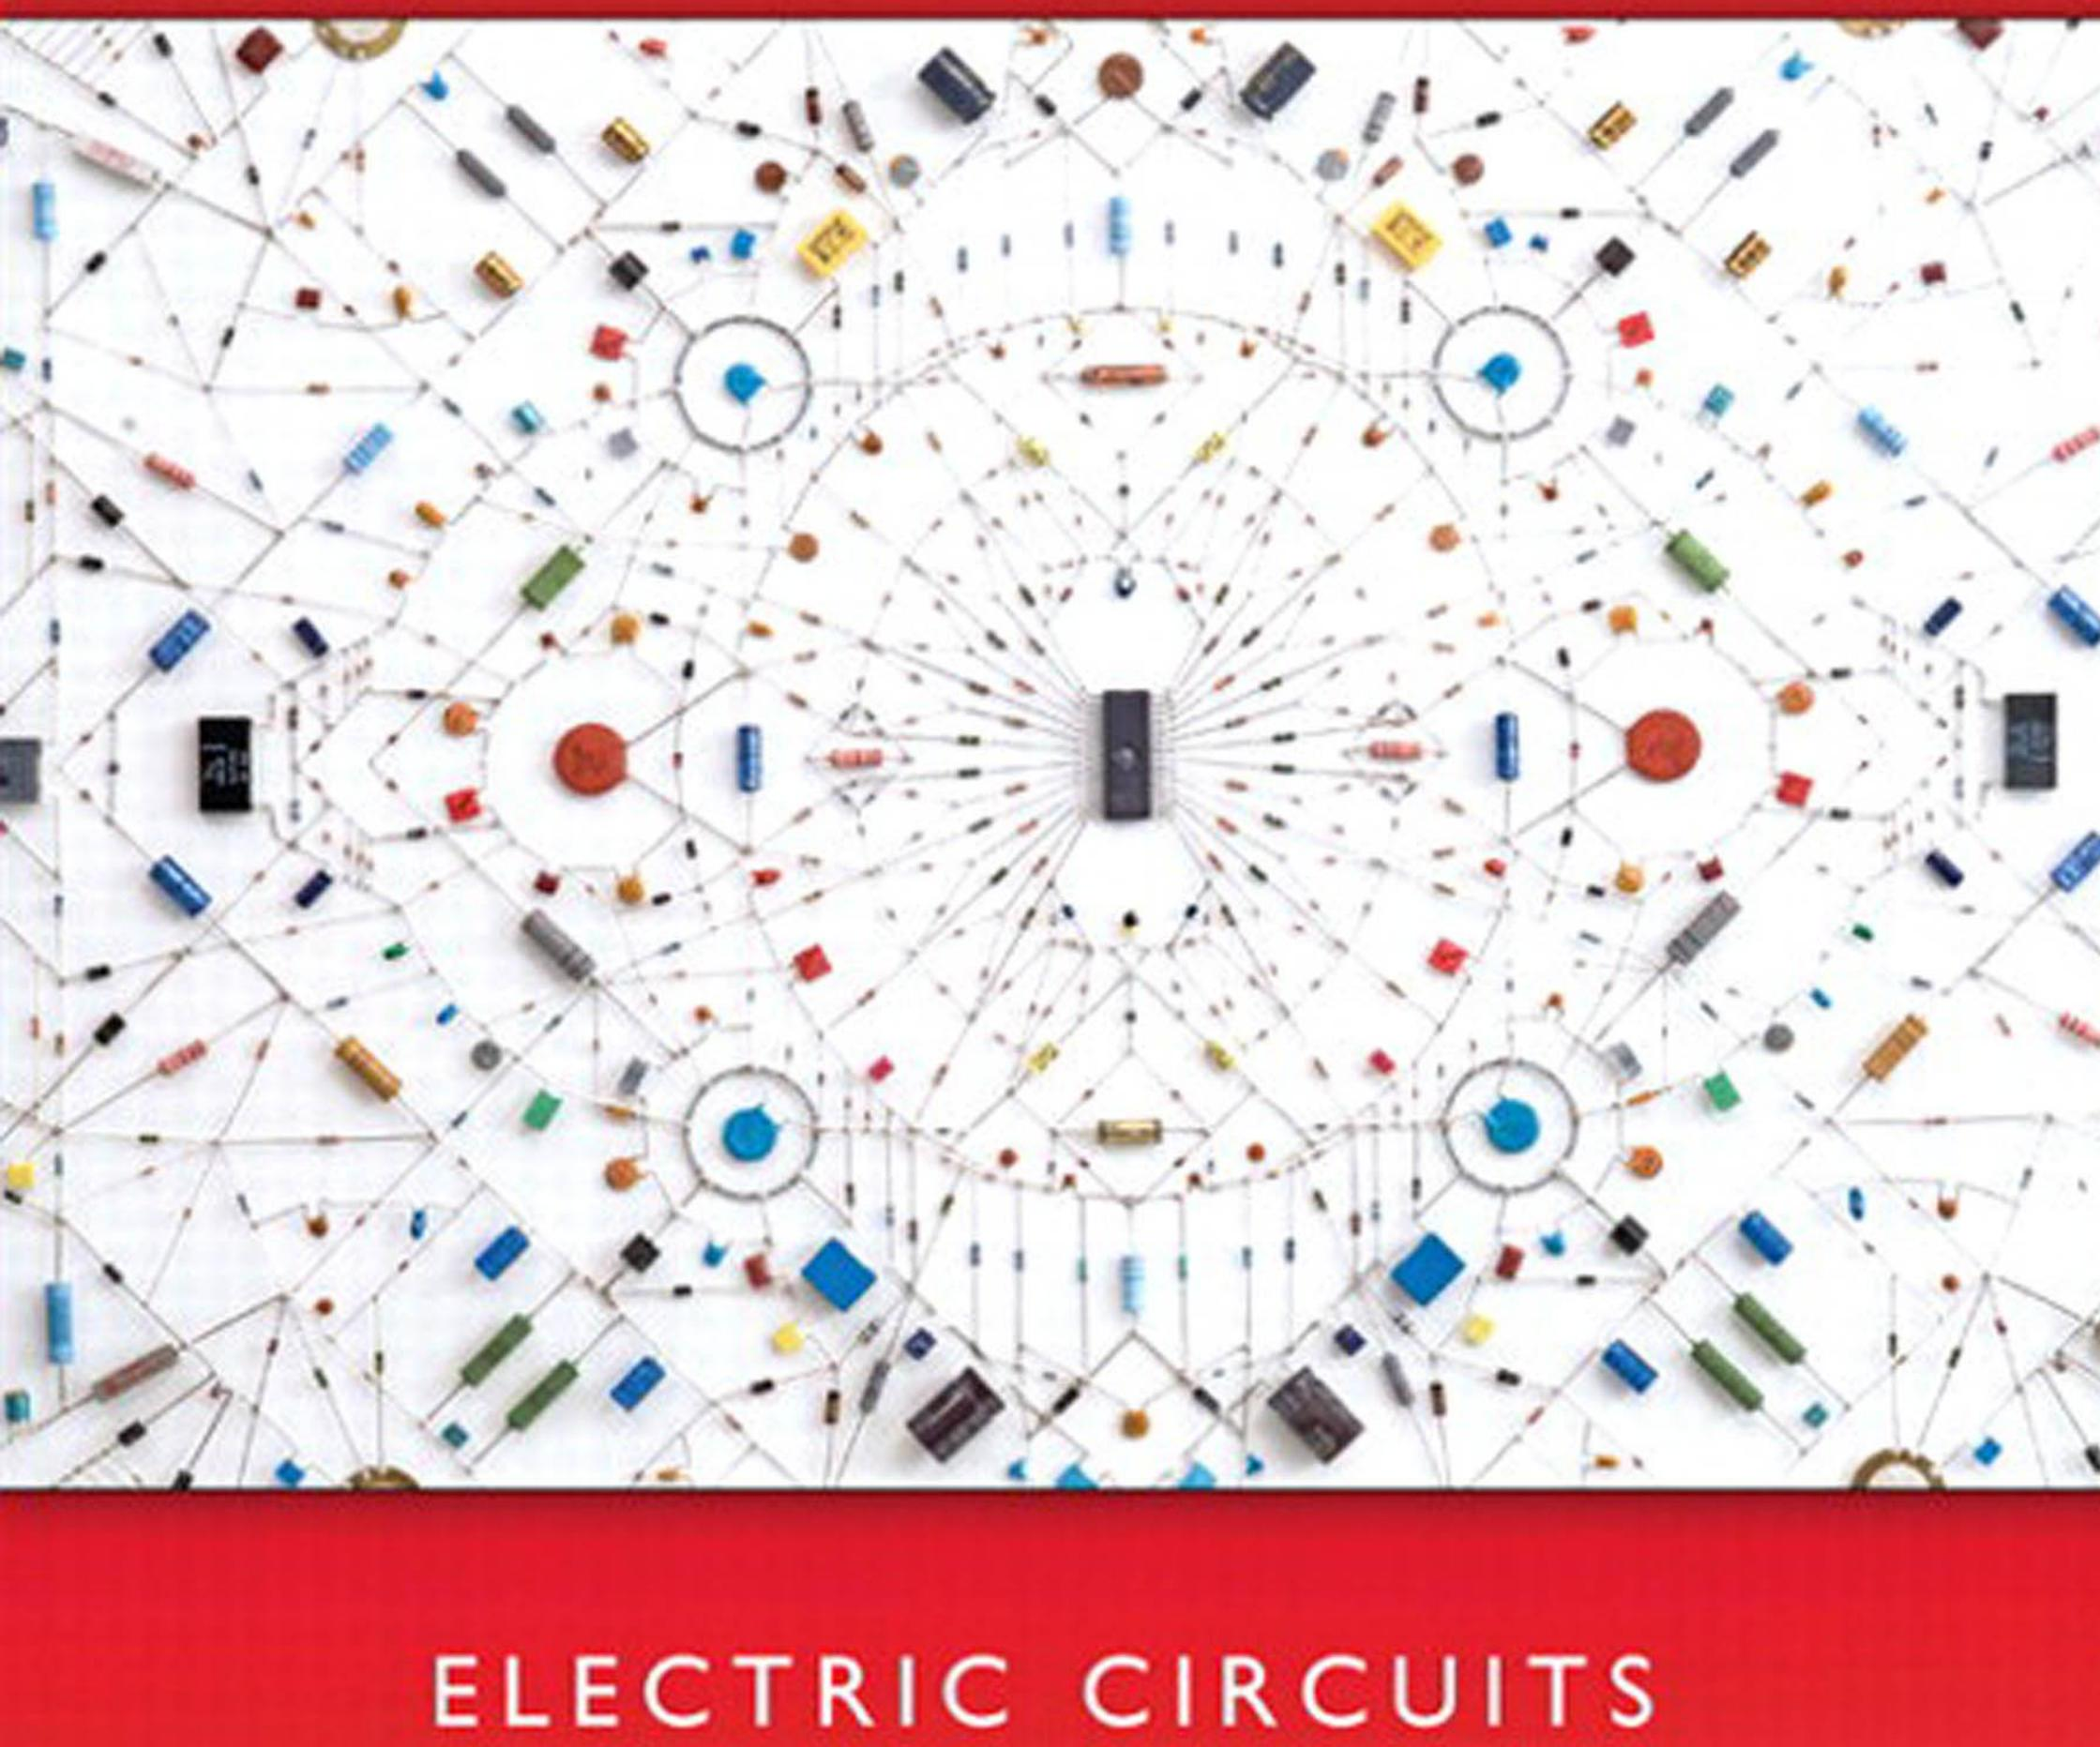
\includegraphics[max width=\textwidth]{2024_10_28_c0e2dc6a235cac59ec77g-001}
\end{center}

10th Edition

\section*{A List of Tables}
Table No. Title Page No.\\
1.1 The International System of Units (SI) ..... 9\\
1.2 Derived Units in SI ..... 9\\
1.3 Standardized Prefixes to Signify Powers of 10 ..... 9\\
1.4 Interpretation of Reference Directions in Fig. 1.5 ..... 13\\
4.1 Terms for Describing Circuits ..... 91\\
4.2 PSpice Sensitivity Analysis Results ..... 128\\
6.1 Terminal Equations for Ideal Inductors and Capacitors ..... 203\\
6.2 Equations for Series- and Parallel-Connected Inductors and Capacitors ..... 203\\
7.1 Value of $e^{-t / \tau}$ for $t$ Equal to Integral Multiples of $\tau$ ..... 217\\
8.1 Natural Response Parameters of the Parallel RLC Circuit ..... 269\\
8.2 The Response of a Second-Order Circuit is Overdamped, Underdamped, or Critically Damped ..... 295\\
8.3 In Determining the Natural Response of a Second-Order Circuit, We First Determine Whether it is Over-, Under-, or Critically Damped, and Then We Solve the Appropriate Equations ..... 295\\
8.4 In Determining the Step Response of a Second-Order Circuit, We Apply the Appropriate Equations Depending on the Damping ..... 296\\
9.1 Impedance and Reactance Values ..... 318\\
9.2 Admittance and Susceptance Values ..... 322\\
9.3 Impedance and Related Values ..... 345\\
10.1 Annual Energy Requirements of Electric Household Appliances ..... 365\\
$10.2 \quad$ Three Power Quantities and Their Units ..... 368\\
12.1 An Abbreviated List of Laplace Transform Pairs ..... 435\\
12.2 An Abbreviated List of Operational Transforms ..... 440\\
$12.3 \quad$ Four Useful Transform Pairs ..... 451\\
13.1 Summary of the $s$-Domain Equivalent Circuits ..... 468\\
13.2 Numerical Values of $v_{o}(t)$ ..... 492\\
14.1 Input and Output Voltage Magnitudes for Several Frequencies ..... 527\\
15.1 Normalized (so that $\omega_{c}=1 \mathrm{rad} / \mathrm{s}$ ) Butterworth Polynomials up to the Eighth Order ..... 577\\
17.1 Fourier Transforms of Elementary Functions ..... 653\\
17.2 Operational Transforms ..... 658\\
18.1 Parameter Conversion Table ..... 682\\
18.2 Terminated Two-Port Equations ..... 688

\begin{center}
\begin{tabular}{|c|c|c|c|c|c|c|c|c|}
\hline
\multicolumn{9}{|c|}{Greek Alphabet} \\
\hline
A & $\alpha$ & Alpha & I & っ & Iota & P & $\rho$ & Rho \\
\hline
B & $\beta$ & Beta & K & $\kappa$ & Kappa & $\Sigma$ & $\sigma$ & Sigma \\
\hline
$\Gamma$ & $\gamma$ & Gamma & $\Lambda$ & $\lambda$ & Lambda & T & $\tau$ & Tau \\
\hline
$\Delta$ & $\delta$ & Delta & M & $\mu$ & Mu & Y & $v$ & Upsilon \\
\hline
E & $\epsilon$ & Epsilon & N & $\nu$ & Nu & $\Phi$ & $\phi$ & Phi \\
\hline
Z & $\zeta$ & Zeta & 泣 & $\xi$ & Xi & X & $\chi$ & Chi \\
\hline
H & $\eta$ & Eta & O & o & Omicron & $\Psi$ & $\psi$ & Psi \\
\hline
Ө & $\theta$ & Theta & $\Pi$ & $\pi$ & Pi & $\Omega$ & $\omega$ & Omega \\
\hline
\end{tabular}
\end{center}

\section*{ELECTRIC CIRCUITS}
TENTH EDITION

This page intentionally left blank

\section*{ELECTRIC CIRCUITS }
TENTH EDITION

Professor Emeritus\\
Iowa State University

\section*{Susan A. Riedel}
Marquette University

\section*{PEARSON}
Boston Columbus Indianapolis New York San Francisco Upper Saddle River Amsterdam Cape Town Dubai London Madrid Milan Munich Paris Montréal Toronto Delhi Mexico City São Paulo Sydney Hong Kong Seoul Singapore Taipei Tokyo

Vice President and Editorial Director:\\
Marcia J. Horton\\
Executive Editor: Andrew Gilfillan\\
Editorial Assistant: Sandra Rodriguez\\
Marketing Manager: Tim Galligan\\
Senior Managing Editor: Scott Disanno\\
Production Editor: Rose Kernan

Cover Design: Black Horse Designs\\
Cover Art: Inverter 04 Oil painting by Ben Leone\\
"TechScape" Collection. \href{http://www.benleone.com}{www.benleone.com}\\
Manager, Cover Visual Research \& Permissions:\\
Karen Sanatar\\
Photo Researcher: Marta Samsel\\
Composition: Integra Publishing Services

Credits and acknowledgments borrowed from other sources and reproduced, with permission, in this textbook appear on appropriate page within text.

\section*{Copyright © 2015, 2008, 2005 Pearson Education, Inc., publishing as Prentice Hall, One Lake Street,}
Upper Saddle River, New Jersey, 07458. All rights reserved. Manufactured in the United States of America. This publication is protected by Copyright, and permission should be obtained from the publisher prior to any prohibited reproduction, storage in a retrieval system, or transmission in any form or by any means, electronic, mechanical, photocopying, recording, or likewise. To obtain permission(s) to use material from this work, please submit a written request to Pearson Education, Inc., Permissions Department, One Lake Street, Upper Saddle River, New Jersey, 07458 .

\section*{Library of Congress Cataloging-in-Publication Data}
Nilsson, James William.\\
Electric circuits / James W. Nilsson, Professor Emeritus, Iowa State University, Susan A. Riedel, Marquette University. - Tenth edition.\\
pages cm\\
ISBN-13: 978-0-13-376003-3\\
ISBN-10: 0-13-376003-0

\begin{enumerate}
  \item Electric circuits. I. Riedel, Susan A. II. Title.
\end{enumerate}

TK545.N54 2015\\
621.319 '2-dc23

To Anna

This page intentionally left blank

\section*{Brief Contents}
List of Examples ..... xiii\\
Preface ..... xvii\\
Chapter 1 Circuit Variables ..... 2\\
Chapter 2 Circuit Elements ..... 24\\
Chapter 3 Simple Resistive Circuits ..... 56\\
Chapter 4 Techniques of Circuit Analysis ..... 88\\
Chapter 5 The Operational Amplifier ..... 144\\
Chapter 6 Inductance, Capacitance, and Mutual Inductance ..... 174\\
Chapter 7 Response of First-Order RL and RC Circuits ..... 212\\
Chapter $8 \quad$ Natural and Step Responses of RLC Circuits ..... 264\\
Chapter 9 Sinusoidal Steady-State Analysis ..... 304\\
Chapter 10 Sinusoidal Steady-State Power Calculations ..... 358\\
Chapter 11 Balanced Three-Phase Circuits ..... 396\\
Chapter 12 Introduction to the Laplace Transform ..... 426\\
Chapter 13 The Laplace Transform in Circuit Analysis ..... 464\\
Chapter 14 Introduction to Frequency Selective Circuits ..... 520\\
Chapter 15 Active Filter Circuits ..... 556\\
Chapter 16 Fourier Series ..... 602\\
Chapter 17 The Fourier Transform ..... 642\\
Chapter 18 Two-Port Circuits ..... 676\\
Appendix A The Solution of Linear Simultaneous Equations ..... 703\\
Appendix B Complex Numbers ..... 723\\
Appendix C More on Magnetically Coupled Coils and Ideal Transformers ..... 729\\
Appendix D The Decibel ..... 737\\
Appendix E Bode Diagrams ..... 739\\
Appendix F An Abbreviated Table of Trigonometric Identities ..... 757\\
Appendix G An Abbreviated Table of Integrals ..... 759\\
Appendix H Common Standard Component Values ..... 761\\
Answers to Selected Problems ..... 763\\
Index ..... 775

This page intentionally left blank

\section*{Contents}
List of Examples ..... xiii\\
Preface ..... xvii\\
Chapter 1 Circuit Variables ..... 2\\
Practical Perspective: Balancing Power ..... 3\\
1.1 Electrical Engineering: An Overview ..... 4\\
1.2 The International System of Units ..... 8\\
1.3 Circuit Analysis: An Overview ..... 10\\
1.4 Voltage and Current ..... 11\\
1.5 The Ideal Basic Circuit Element ..... 12\\
1.6 Power and Energy ..... 14\\
Practical Perspective: Balancing Power ..... 17\\
Summary ..... 18\\
Problems ..... 19\\
Chapter 2 Circuit Elements ..... 24\\
Practical Perspective: Heating with ElectricRadiators25\\
2.1 Voltage and Current Sources ..... 26\\
2.2 Electrical Resistance (Ohm's Law) ..... 30\\
2.3 Construction of a Circuit Model ..... 34\\
2.4 Kirchhoff's Laws ..... 37\\
2.5 Analysis of a Circuit Containing Dependent Sources ..... 42\\
Practical Perspective: Heating with Electric Radiators 46\\
Summary ..... 48\\
Problems ..... 48\\
Chapter 3 Simple Resistive Circuits ..... 56\\
Practical Perspective: Resistive Touch\\
Screens ..... 57\\
3.1 Resistors in Series ..... 58\\
3.2 Resistors in Parallel ..... 59\\
3.3 The Voltage-Divider and Current-Divider Circuits ..... 61\\
3.4 Voltage Division and Current Division ..... 64\\
3.5 Measuring Voltage and Current ..... 66\\
3.6 Measuring Resistance-The Wheatstone Bridge ..... 69\\
3.7 Delta-to-Wye (Pi-to-Tee) EquivalentCircuits71\\
Practical Perspective: Resistive Touch\\
Screens ..... 73\\
Summary ..... 75\\
Problems ..... 76\\
Chapter 4 Techniques of Circuit Analysis ..... 88\\
Practical Perspective: Circuits with Realistic\\
Resistors ..... 89\\
4.1 Terminology ..... 90\\
4.2 Introduction to the Node-Voltage Method ..... 93\\
4.3 The Node-Voltage Method and Dependent Sources ..... 95\\
4.4 The Node-Voltage Method: Some Special Cases ..... 96\\
4.5 Introduction to the Mesh-Current Method ..... 99\\
4.6 The Mesh-Current Method and Dependent Sources ..... 102\\
4.7 The Mesh-Current Method: Some Special Cases ..... 103\\
4.8 The Node-Voltage Method Versus the Mesh-Current Method ..... 106\\
4.9 Source Transformations ..... 109\\
4.10 Thévenin and Norton Equivalents ..... 113\\
4.11 More on Deriving a Thévenin Equivalent ..... 117\\
4.12 Maximum Power Transfer ..... 120\\
4.13 Superposition ..... 122\\
Practical Perspective: Circuits with RealisticResistors125\\
Summary ..... 129\\
Problems ..... 130\\
Chapter 5 The Operational Amplifier ..... 144\\
Practical Perspective: Strain Gages ..... 145\\
5.1 Operational Amplifier Terminals ..... 146\\
5.2 Terminal Voltages and Currents ..... 146\\
5.3 The Inverting-Amplifier Circuit ..... 150\\
5.4 The Summing-Amplifier Circuit ..... 152\\
5.5 The Noninverting-Amplifier Circuit ..... 153\\
5.6 The Difference-Amplifier Circuit ..... 155\\
5.7 A More Realistic Model for the Operational Amplifier ..... 159\\
Practical Perspective: Strain\\
Gages ..... 162\\
Summary ..... 164\\
Problems ..... 165\\
Chapter 6 Inductance, Capacitance, and Mutual Inductance ..... 174\\
Practical Perspective: Capacitive Touch\\
Screens ..... 175\\
6.1 The Inductor ..... 176\\
6.2 The Capacitor ..... 182\\
6.3 Series-Parallel Combinations of Inductance and Capacitance ..... 187\\
6.4 Mutual Inductance ..... 189\\
6.5 A Closer Look at Mutual Inductance ..... 193\\
Practical Perspective: Capacitive Touch\\
Screens ..... 200\\
Summary ..... 202\\
Problems ..... 204\\
Chapter 7 Response of First-Order RL and RC Circuits ..... 212\\
Practical Perspective: Artificial Pacemaker ..... 213\\
7.1 The Natural Response of an RL Circuit ..... 214\\
7.2 The Natural Response of an RC Circuit ..... 220\\
7.3 The Step Response of RL and RC Circuits ..... 224\\
7.4 A General Solution for Step and Natural Responses ..... 231\\
7.5 Sequential Switching ..... 236\\
7.6 Unbounded Response ..... 240\\
7.7 The Integrating Amplifier ..... 241\\
Practical Perspective: Artificial Pacemaker ..... 245\\
Summary ..... 246\\
Problems ..... 247\\
Chapter 8 Natural and Step Responses of RLC Circuits ..... 264\\
Practical Perspective: Clock for Computer Timing ..... 265\\
8.1 Introduction to the Natural Response of a Parallel RLC Circuit ..... 266\\
8.2 The Forms of the Natural Response of a Parallel RLC Circuit ..... 270\\
8.3 The Step Response of a Parallel RLC Circuit ..... 280\\
8.4 The Natural and Step Response of a Series RLC Circuit ..... 285\\
8.5 A Circuit with Two Integrating Amplifiers ..... 289\\
Practical Perspective: Clock for Computer\\
Timing ..... 293\\
Summary ..... 295\\
Problems ..... 296\\
Chapter 9 Sinusoidal Steady-State Analysis ..... 304\\
Practical Perspective: A Household DistributionCircuit 305\\
9.1 The Sinusoidal Source ..... 306\\
9.2 The Sinusoidal Response ..... 309\\
9.3 The Phasor ..... 310\\
9.4 The Passive Circuit Elements in the Frequency Domain ..... 315\\
9.5 Kirchhoff's Laws in the Frequency Domain ..... 319\\
9.6 Series, Parallel, and Delta-to-Wye Simplifications ..... 320\\
9.7 Source Transformations and Thévenin-Norton Equivalent Circuits ..... 327\\
9.8 The Node-Voltage Method ..... 330\\
9.9 The Mesh-Current Method ..... 331\\
9.10 The Transformer ..... 332\\
9.11 The Ideal Transformer ..... 336\\
9.12 Phasor Diagrams ..... 342\\
Practical Perspective: A Household Distribution\\
Circuit ..... 344\\
Summary ..... 345\\
Problems ..... 346\\
Chapter 10 Sinusoidal Steady-State Power Calculations ..... 358\\
Practical Perspective: Vampire\\
Power ..... 359\\
10.1 Instantaneous Power ..... 360\\
10.2 Average and Reactive Power ..... 361\\
10.3 The rms Value and Power Calculations ..... 366\\
10.4 Complex Power ..... 368\\
10.5 Power Calculations ..... 369\\
10.6 Maximum Power Transfer ..... 376\\
Practical Perspective: Vampir\\
Power ..... 382\\
Summary ..... 384\\
Problems ..... 385\\
Chapter 11 Balanced Three-Phase Circuits ..... 396\\
Practical Perspective: Transmission andDistribution of Electric Power 397\\
11.1 Balanced Three-Phase Voltages ..... 398\\
11.2 Three-Phase Voltage Sources ..... 399\\
11.3 Analysis of the Wye-Wye Circuit ..... 400\\
11.4 Analysis of the Wye-Delta Circuit ..... 405\\
11.5 Power Calculations in Balanced Three-Phase Circuits ..... 408\\
11.6 Measuring Average Power in Three-Phase Circuits ..... 413\\
Practical Perspective: Transmission and\\
Distribution of Electric Power ..... 416\\
Summary ..... 417\\
Problems ..... 418\\
Chapter 12 Introduction to the Laplace Transform ..... 426\\
Practical Perspective: Transient Effects ..... 427\\
12.1 Definition of the Laplace Transform ..... 428\\
12.2 The Step Function ..... 429\\
12.3 The Impulse Function ..... 431\\
12.4 Functional Transforms ..... 434\\
12.5 Operational Transforms ..... 435\\
12.6 Applying the Laplace Transform ..... 440\\
12.7 Inverse Transforms ..... 442\\
12.8 Poles and Zeros of $F(s)$ ..... 452\\
12.9 Initial- and Final-Value Theorems ..... 453\\
Practical Perspective: Transient\\
Effects ..... 456\\
Summary ..... 457\\
Problems ..... 458\\
Chapter 13 The Laplace Transform in Circuit Analysis ..... 464\\
Practical Perspective: Surge Suppressors ..... 465\\
13.1 Circuit Elements in the $s$ Domain ..... 466\\
13.2 Circuit Analysis in the $s$ Domain ..... 468\\
13.3 Applications ..... 470\\
13.4 The Transfer Function ..... 482\\
13.5 The Transfer Function in Partial Fraction Expansions ..... 484\\
13.6 The Transfer Function and the Convolution Integral ..... 487\\
13.7 The Transfer Function and the Steady-State Sinusoidal Response ..... 493\\
13.8 The Impulse Function in Circuit Analysis ..... 496\\
Practical Perspective: Surge Suppressors ..... 503\\
Summary ..... 504\\
Problems ..... 505\\
Chapter 14 Introduction to Frequency Selective Circuits ..... 520\\
Practical Perspective: Pushbutton Telephone Circuits ..... 521\\
14.1 Some Preliminaries ..... 522\\
14.2 Low-Pass Filters ..... 524\\
14.3 High-Pass Filters ..... 530\\
14.4 Bandpass Filters ..... 534\\
14.5 Bandreject Filters ..... 543\\
Practical Perspective: Pushbutton Telephone\\
Circuits ..... 548\\
Summary ..... 548\\
Problems ..... 549\\
Chapter 15 Active Filter Circuits ..... 556Practical Perspective: Bass VolumeControl 557\\
15.1 First-Order Low-Pass and High-Pass Filters ..... 558\\
15.2 Scaling ..... 562\\
15.3 Op Amp Bandpass and Bandreject Filters ..... 564\\
15.4 Higher Order Op Amp Filters ..... 571\\
15.5 Narrowband Bandpass and BandrejectFilters584\\
Practical Perspective: Bass Volume Control ..... 589\\
Summary ..... 592\\
Problems ..... 593\\
Chapter 16 Fourier Series ..... 602\\
Practical Perspective: Active High-Q Filters ..... 603\\
16.1 Fourier Series Analysis: An Overview ..... 605\\
16.2 The Fourier Coefficients ..... 606\\
16.3 The Effect of Symmetry on the Fourier Coefficients ..... 609\\
16.4 An Alternative Trigonometric Form of the Fourier Series ..... 615\\
16.5 An Application ..... 617\\
16.6 Average-Power Calculations with Periodic Functions ..... 621\\
16.7 The rms Value of a Periodic Function ..... 624\\
16.8 The Exponential Form of the Fourier Series ..... 625\\
16.9 Amplitude and Phase Spectra ..... 628\\
Practical Perspective: Active High-Q Filters ..... 630\\
Summary ..... 632\\
Problems ..... 633\\
Chapter 17 The Fourier Transform ..... 642Practical Perspective: Filtering DigitalSignals 643\\
17.1 The Derivation of the Fourier Transform ..... 644\\
17.2 The Convergence of the Fourier Integral ..... 646\\
17.3 Using Laplace Transforms to Find Fourier Transforms ..... 648\\
17.4 Fourier Transforms in the Limit ..... 651\\
17.5 Some Mathematical Properties ..... 653\\
17.6 Operational Transforms ..... 655\\
17.7 Circuit Applications ..... 659\\
17.8 Parseval's Theorem ..... 662\\
Practical Perspective: Filtering Digital Signals ..... 669\\
Summary ..... 670\\
Problems ..... 670\\
Chapter 18 Two-Port Circuits ..... 676\\
Practical Perspective: Characterizing anUnknown Circuit677\\
18.1 The Terminal Equations ..... 678\\
18.2 The Two-Port Parameters ..... 679\\
18.3 Analysis of the Terminated Two-Port Circuit ..... 687\\
18.4 Interconnected Two-Port Circuits ..... 692\\
Practical Perspective: Characterizing an Unknown Circuit ..... 695\\
Summary ..... 696\\
Problems ..... 696\\
Appendix A The Solution of Linear Simultaneous Equations ..... 703\\
A. 1 Preliminary Steps ..... 703\\
A. 2 Cramer's Method ..... 704\\
A. 3 The Characteristic Determinant ..... 704\\
A. 4 The Numerator Determinant ..... 704\\
A. 5 The Evaluation of a Determinant ..... 705\\
A. 6 Matrices ..... 707\\
A. 7 Matrix Algebra ..... 708\\
A. 8 Identity, Adjoint, and Inverse Matrices ..... 712\\
A. 9 Partitioned Matrices ..... 715\\
A. 10 Applications ..... 718\\
Appendix B Complex Numbers ..... 723\\
B. 1 Notation ..... 723\\
B. 2 The Graphical Representation of a Complex Number ..... 724\\
B. 3 Arithmetic Operations ..... 725\\
B. 4 Useful Identities ..... 726\\
B. 5 The Integer Power of a Complex Number ..... 727\\
B. 6 The Roots of a Complex Number ..... 727\\
Appendix C More on Magnetically Coupled Coils and Ideal Transformers ..... 729\\
C. 1 Equivalent Circuits for Magnetically Coupled Coils ..... 729\\
C. 2 The Need for Ideal Transformers in the Equivalent Circuits ..... 733\\
Appendix D The Decibel ..... 737\\
Appendix E Bode Diagrams ..... 739\\
E. 1 Real, First-Order Poles and Zeros ..... 739\\
E. 2 Straight-Line Amplitude Plots ..... 740\\
E. 3 More Accurate Amplitude Plots ..... 744\\
E. 4 Straight-Line Phase Angle Plots ..... 745\\
E. 5 Bode Diagrams: Complex Poles and Zeros ..... 747\\
E. 6 Amplitude Plots ..... 749\\
E. 7 Correcting Straight-Line Amplitude Plots ..... 750\\
E. 8 Phase Angle Plots ..... 753\\
Appendix F An Abbreviated Table of Trigonometric Identities ..... 757\\
Appendix G An Abbreviated Table of Integrals ..... 759\\
Appendix H Common Standard Component Values ..... 761\\
Answers to Selected Problems ..... 763\\
Index ..... 775

\section*{List of Examples}
Chapter 1\\
1.1 Using SI Units and Prefixes for Powers of 10 ..... 10\\
1.2 Relating Current and Charge ..... 14\\
1.3 Relating Voltage, Current, Power, and Energy ..... 16\\
Chapter 2\\
2.1 Testing Interconnections of Ideal Sources ..... 28\\
2.2 Testing Interconnections of Ideal Independent and Dependent Sources ..... 29\\
2.3 Calculating Voltage, Current, and Power for a Simple Resistive Circuit ..... 33\\
2.4 Constructing a Circuit Model of a Flashlight ..... 34\\
2.5 Constructing a Circuit Model Based on Terminal Measurements ..... 36\\
2.6 Using Kirchhoff's Current Law ..... 39\\
2.7 Using Kirchhoff's Voltage Law ..... 40\\
2.8 Applying Ohm's Law and Kirchhoff's Laws to Find an Unknown Current ..... 40\\
2.9 Constructing a Circuit Model Based on Terminal Measurements ..... 41\\
2.10 Applying Ohm's Law and Kirchhoff's Laws to Find an Unknown Voltage ..... 44\\
2.11 Applying Ohm's Law and Kirchhoff's Law in an Amplifier Circuit ..... 45\\
Chapter 3\\
3.1 Applying Series-Parallel Simplification ..... 60\\
3.2 Analyzing the Voltage-Divider Circuit ..... 62\\
3.3 Analyzing a Current-Divider Circuit ..... 63\\
3.4 Using Voltage Division and Current Division to Solve a Circuit ..... 66\\
3.5 Using a d'Arsonval Ammeter ..... 68\\
3.6 Using a d'Arsonval Voltmeter ..... 68\\
3.7 Applying a Delta-to-Wye Transform ..... 72\\
Chapter 4\\
4.1 Identifying Node, Branch, Mesh and Loop in a Circuit ..... 90\\
4.2 Using the Node-Voltage Method ..... 94\\
4.3 Using the Node-Voltage Method with Dependent Sources ..... 95\\
4.4 Using the Mesh-Current Method ..... 101\\
4.5 Using the Mesh-Current Method with Dependent Sources ..... 102\\
4.6 Understanding the Node-Voltage Method Versus Mesh-Current Method ..... 107\\
4.7 Comparing the Node-Voltage and Mesh-Current Methods ..... 108\\
4.8 Using Source Transformations to Solve a Circuit ..... 110\\
4.9 Using Special Source Transformation Techniques ..... 112\\
4.10 Finding the Thévenin Equivalent of a Circuit with a Dependent Source ..... 116\\
4.11 Finding the Thévenin Equivalent Using a Test Source ..... 118\\
4.12 Calculating the Condition for Maximum Power Transfer ..... 121\\
4.13 Using Superposition to Solve a Circuit ..... 124\\
Chapter 5\\
5.1 Analyzing an Op Amp Circuit ..... 149\\
5.2 Designing an Inverting Amplifier ..... 151\\
5.3 Designing a Noninverting Amplifier ..... 154\\
5.4 Designing a Difference Amplifier ..... 155\\
Chapter 6\\
6.1 Determining the Voltage, Given the Current, at the Terminals of an Inductor ..... 177\\
6.2 Determining the Current, Given the Voltage, at the Terminals of an Inductor ..... 178\\
6.3 Determining the Current, Voltage, Power, and Energy for an Inductor ..... 180\\
6.4 Determining Current, Voltage, Power, and Energy for a Capacitor ..... 184\\
6.5 Finding $v, p$, and $w$ Induced by a Triangular Current Pulse for a Capacitor ..... 185\\
6.6 Finding Mesh-Current Equations for a Circuit with Magnetically Coupled Coils ..... 192\\
Chapter 7\\
7.1 Determining the Natural Response of an RL Circuit ..... 218\\
7.2 Determining the Natural Response of an RL Circuit with Parallel Inductors ..... 219\\
7.3 Determining the Natural Response of an RC Circuit ..... 222\\
7.4 Determining the Natural Response of an $R C$ Circuit with Series Capacitors ..... 223\\
7.5 Determining the Step Response of anRL Circuit227\\
7.6 Determining the Step Response of an RC Circuit ..... 230\\
7.7 Using the General Solution Method to Find an RC Circuit's Step Response ..... 233\\
7.8 Using the General Solution Method with Zero Initial Conditions ..... 234\\
7.9 Using the General Solution Method to Find an RL Circuit's Step Response ..... 234\\
7.10 Determining the Step Response of a Circuit with Magnetically Coupled Coils ..... 235\\
7.11 Analyzing an RL Circuit that has Sequential Switching ..... 237\\
7.12 Analyzing an RC Circuit that has Sequential Switching ..... 239\\
7.13 Finding the Unbounded Response in an RC Circuit ..... 241\\
7.14 Analyzing an Integrating Amplifier ..... 243\\
7.15 Analyzing an Integrating Amplifier that has Sequential Switching ..... 243\\
Chapter 8\\
8.1 Finding the Roots of the Characteristic Equation of a Parallel RLC Circuit ..... 269\\
8.2 Finding the Overdamped Natural Response of a Parallel RLC Circuit ..... 272\\
8.3 Calculating Branch Currents in the Natural Response of a Parallel RLC Circuit ..... 273\\
8.4 Finding the Underdamped Natural Response of a Parallel RLC Circuit ..... 275\\
8.5 Finding the Critically Damped Natural Response of a Parallel RLC Circuit ..... 278\\
8.6 Finding the Overdamped Step Response of a Parallel RLC Circuit ..... 282\\
8.7 Finding the Underdamped Step Response of a Parallel RLC Circuit ..... 283\\
8.8 Finding the Critically Damped Step Response of a Parallel RLC Circuit ..... 283\\
8.9 Comparing the Three-Step Response Forms ..... 284\\
8.10 Finding Step Response of a Parallel RLC Circuit with Initial Stored Energy ..... 284\\
8.11 Finding the Underdamped Natural Response of a Series RLC Circuit ..... 287\\
8.12 Finding the Underdamped Step Response of a Series RLC Circuit ..... 288\\
8.13 Analyzing Two Cascaded Integrating Amplifiers ..... 290\\
8.14 Analyzing Two Cascaded Integrating Amplifiers with Feedback Resistors ..... 293

\section*{Chapter 9}
\subsection*{9.1 Finding the Characteristics of a Sinusoidal Current \\
 307}
9.2 Finding the Characteristics of a Sinusoidal Voltage ..... 308\\
9.3 Translating a Sine Expression to a Cosine Expression ..... 308\\
9.4 Calculating the rms Value of a Triangular Waveform ..... 308\\
9.5 Adding Cosines Using Phasors ..... 314\\
9.6 Combining Impedances in Series ..... 321\\
9.7 Combining Impedances in Series and in Parallel ..... 323\\
9.8 Using a Delta-to-Wye Transform in the Frequency Domain ..... 325\\
9.9 Performing Source Transformations in the Frequency Domain ..... 327\\
9.10 Finding a Thévenin Equivalent in the Frequency Domain ..... 328\\
9.11 Using the Node-Voltage Method in the Frequency Domain ..... 330\\
9.12 Using the Mesh-Current Method in the Frequency Domain ..... 331\\
9.13 Analyzing a Linear Transformer in the Frequency Domain ..... 335\\
9.14 Analyzing an Ideal Transformer Circuit in the Frequency Domain ..... 340\\
9.15 Using Phasor Diagrams to Analyze a Circuit ..... 342\\
9.16 Using Phasor Diagrams to Analyze Capacitive Loading Effects ..... 343\\
Chapter 10\\
10.1 Calculating Average and Reactive Power ..... 364\\
10.2 Making Power Calculations Involving Household Appliances ..... 365\\
10.3 Determining Average Power Delivered to a Resistor by Sinusoidal Voltage ..... 367\\
10.4 Calculating Complex Power ..... 369\\
10.5 Calculating Average and Reactive Power ..... 372\\
10.6 Calculating Power in Parallel Loads ..... 373\\
10.7 Balancing Power Delivered with Power Absorbed in an ac Circuit ..... 374\\
10.8 Determining Maximum Power Transfer without Load Restrictions ..... 378\\
10.9 Determining Maximum Power Transfer with Load Impedance Restriction ..... 379\\
10.10 Finding Maximum Power Transfer withImpedance Angle Restrictions 380\\
10.11 Finding Maximum Power Transfer in a Circuitwith an Ideal Transformer 381

\section*{Chapter 11}
11.1 Analyzing a Wye-Wye Circuit 403\\
11.2 Analyzing a Wye-Delta Circuit 406\\
11.3 Calculating Power in a Three-Phase Wye-Wye Circuit 411\\
11.4 Calculating Power in a Three-Phase Wye-Delta\\
Circuit 411\\
11.5 Calculating Three-Phase Power with\\
an Unspecified Load 412\\
11.6 Computing Wattmeter Readings in Three-Phase Circuits 415

\section*{Chapter 12}
\subsection*{12.1 Using Step Functions to Represent a Function of Finite Duration 430}
\section*{Chapter 13}
13.1 Deriving the Transfer Function of a Circuit 483\\
13.2 Analyzing the Transfer Function of a Circuit 485\\
13.3 Using the Convolution Integral to Find an Output Signal 491\\
13.4 Using the Transfer Function to Find the Steady-State Sinusoidal Response ..... 495\\
Chapter 14\\
14.1 Designing a Low-Pass Filter ..... 527\\
14.2 Designing a Series RC Low-Pass Filter ..... 528\\
14.3 Designing a Series RL High-Pass Filter ..... 532\\
14.4 Loading the Series RL High-Pass Filter ..... 532\\
14.5 Designing a Bandpass Filter ..... 538\\
14.6 Designing a Parallel RLC Bandpass Filter ..... 539\\
14.7 Determining Effect of a Nonideal Voltage Source on a RLC Bandpass Filter ..... 540\\
14.8 Designing a Series RLC Bandreject Filter ..... 546\\
Chapter 15\\
15.1 Designing a Low-Pass Op Amp Filter ..... 559\\
15.2 Designing a High-Pass Op Amp Filter ..... 561\\
15.3 Scaling a Series RLC Circuit ..... 563\\
15.4 Scaling a Prototype Low-Pass 0p Amp Filter ..... 563\\
15.5 Designing a Broadband Bandpass 0p Amp Filter ..... 567\\
15.6 Designing a Broadband Bandreject Op Amp Filter ..... 570\\
15.7 Designing a Fourth-Order Low-Pass Op Amp Filter ..... 574\\
15.8 Calculating Butterworth Transfer Functions ..... 577\\
15.9 Designing a Fourth-Order Low-Pass Butterworth Filter ..... 579\\
15.10 Determining the Order of a Butterworth Filter ..... 582\\
15.11 An Alternate Approach to Determining the Order of a Butterworth Filter ..... 582\\
15.12 Designing a High-Q Bandpass Filter ..... 586\\
15.13 Designing a High-Q Bandreject Filter ..... 588\\
Chapter 16\\
16.1 Finding the Fourier Series of a Triangular Waveform with No Symmetry ..... 607\\
16.2 Finding the Fourier Series of an Odd Function with Symmetry ..... 614\\
16.3 Calculating Forms of the Trigonometric Fourier Series for Periodic Voltage ..... 616\\
16.4 Calculating Average Power for a Circuit with a Periodic Voltage Source ..... 623\\
16.5 Estimating the rms Value of a Periodic Function ..... 625\\
16.6 Finding the Exponential Form of the Fourier Series ..... 627\\
Chapter 17\\
17.1 Using the Fourier Transform to Find the Transient Response ..... 660\\
17.2 Using the Fourier Transform to Find the Sinusoidal Steady-State Response ..... 661\\
17.3 Applying Parseval's Theorem ..... 664\\
17.4 Applying Parseval's Theorem to an Ideal Bandpass Filter ..... 665\\
17.5 Applying Parseval's Theorem to a Low-Pass Filter 666\\
Chapter 18\\
18.1 Finding the $z$ Parameters of a Two-Port Circuit ..... 679\\
18.2 Finding the $a$ Parameters from Measurements ..... 681\\
18.3 Finding $h$ Parameters from Measurements and Table 18.1 ..... 684\\
18.4 Analyzing a Terminated Two-Port Circuit ..... 690\\
18.5 Analyzing Cascaded Two-Port Circuits ..... 694

This page intentionally left blank

\section*{Preface}
The first edition of Electric Circuits, an introductory circuits text, was published in 1983. It included 100 worked examples and about 600 problems. It did not include a student workbook, supplements for PSpice or MultiSim, or any web support. Support for instructors was limited to a solution manual for the problems and enlarged copies of many text figures, suitable for making transparencies.

Much has changed in the 31 years since Electric Circuits first appeared, and during that time this text has evolved to better meet the needs of both students and their instructors. As an example, the text now includes about 150 worked examples, about 1850 problems, and extensive supplements and web content. The tenth edition is designed to revise and improve the material presented in the text, in its supplements, and on the web. Yet the fundamental goals of the text are unchanged. These goals are:

\begin{itemize}
  \item To build an understanding of concepts and ideas explicitly in terms of previous learning. Students are constantly challenged by the need to layer new concepts on top of previous concepts they may still be struggling to master. This text provides an important focus on helping students understand how new concepts are related to and rely upon concepts previously presented.
  \item To emphasize the relationship between conceptual understanding and problem-solving approaches. Developing problem-solving skills continues to be the central challenge in a first-year circuits course. In this text we include numerous Examples that present problemsolving techniques followed by Assessment Problems that enable students to test their mastery of the material and techniques introduced. The problem-solving process we illustrate is based on concepts rather than the use of rote procedures. This encourages students to think about a problem before attempting to solve it.
  \item To provide students with a strong foundation of engineering practices. There are limited opportunities in a first-year circuit analysis course to introduce students to realistic engineering experiences. We continue to take advantage of the opportunities that do exist by including problems and examples that use realistic component values and represent realizable circuits. We include many problems related to the Practical Perspective problems that begin each chapter. We also include problems intended to stimulate the students' interest in engineering, where the problems require the type of insight typical of a practicing engineer.
\end{itemize}

\section*{WHY THIS EDITION?}
The tenth edition revision of Electric Circuits began with a thorough review of the text. This review provided a clear picture of what matters most to instructors and their students and led to the following changes:

\begin{itemize}
  \item Problem solving is fundamental to the study of circuit analysis. Having a wealth of new problems to assign and work is a key to success in any circuits course. Therefore, existing end-of-chapter problems were revised, and new end-of-chapter problems were added. As a result, more than $40 \%$ of the problems in the tenth edition have never appeared in any previous edition of the text.
  \item Both students and instructors want to know how the generalized techniques presented in a first-year circuit analysis course relate to problems faced by practicing engineers. The Practical Perspective problems provide this connection between circuit analysis and the real world. We have created new Practical Perspective problems for Chapters 2, 3, 6, 7, 8, and 10. Many of the new problems represent the world of the 21st century. Each Practical Perspective problem is solved, at least in part, at the end of the chapter, and additional end-of-chapter problems can be assigned to allow students to explore the Practical Perspective topic further.
  \item The PSpice and Multisim manuals have been revised to include screenshots from the most recent versions of these software simulation applications. Each manual presents the simulation material in the same order as the material is presented in the text. These manuals continue to include examples of circuits to be simulated that are drawn directly from the text. The text continues to indicate end-ofchapter problems that are good candidates for simulation using either PSpice or Multisim.
  \item Students who could benefit from additional examples and practice problems can use the Student Workbook, which has been revised to reflect changes to the tenth edition of the text. This workbook has examples and problems covering the following material: balancing power, simple resistive circuits, node voltage method, mesh current method, Thévenin and Norton equivalents, op amp circuits, firstorder circuits, second-order circuits, AC steady-state analysis, and Laplace transform circuit analysis.
  \item The Student Workbook now includes access to Video Solutions, complete, step-by-step solution walkthroughs to representative homework problems.
  \item Learning Catalytics, a "bring your own device" student engagement, assessment, and classroom intelligence system is now available with the tenth edition. With Learning Catalytics you can:
  \item Use open-ended questions to get into the minds of students to understand what they do or don't know and adjust lectures accordingly.
  \item Use a wide variety of question types to sketch a graph, annotate a circuit diagram, compose numeric or algebraic answers, and more.
  \item Access rich analytics to understand student performance.
  \item Use pre-built questions or add your own to make Learning Catalytics fit your course exactly.
  \item MasteringEngineering is an online tutorial and assessment program that provides students with personalized feedback and hints and instructors with diagnostics to track students' progress. With the tenth edition, MasteringEngineering will offer new tutorial homework problems, Coaching Activities, and Adaptive Follow-Up assignments. Visit \href{http://www.masteringengineering.com}{www.masteringengineering.com} for more information.
\end{itemize}

\section*{HALLMARK FEATURES}
\section*{Chapter Problems}
Users of Electric Circuits have consistently rated the Chapter Problems as one of the book's most attractive features. In the tenth edition, there are over 1650 end-of-chapter problems with approximately $40 \%$ that have never appeared in a previous edition. Problems are organized at the end of each chapter by section.

\section*{Practical Perspectives}
The tenth edition continues the use of Practical Perspectives introduced with the chapter openers. They offer examples of real-world circuits, taken from real-world devices. The Practical Perspectives for six of the chapters are brand new to this edition. Every chapter begins with a brief description of a practical application of the material that follows. Once the chapter material is presented, the chapter concludes with a quantitative analysis of the Practical Perspective application. A group of end-of-chapter problems directly relates to the Practical Perspective application. Solving some of these problems enables you to understand how to apply the chapter contents to the solution of a real-world problem.

\section*{Assessment Problems}
Each chapter begins with a set of chapter objectives. At key points in the chapter, you are asked to stop and assess your mastery of a particular objective by solving one or more assessment problems. The answers to all of the assessment problems are given at the conclusion of each problem, so you can check your work. If you are able to solve the assessment problems for a given objective, you have mastered that objective. If you need more practice, several end-of-chapter problems that relate to the objective are suggested at the conclusion of the assessment problems.

\section*{Examples}
Every chapter includes many examples that illustrate the concepts presented in the text in the form of a numeric example. There are nearly 150 examples in this text. The examples are intended to illustrate the application of a particular concept, and also to encourage good problem-solving skills.

\section*{Fundamental Equations and Concepts}
Throughout the text, you will see fundamental equations and concepts set apart from the main text. This is done to help you focus on some of the key principles in electric circuits and to help you navigate through the important topics.

\section*{Integration of Computer Tools}
Computer tools can assist students in the learning process by providing a visual representation of a circuit's behavior, validating a calculated solution, reducing the computational burden of more complex circuits, and iterating toward a desired solution using parameter variation. This computational support is often invaluable in the design process. The tenth edition includes the support of PSpice ${ }^{\circledR}$ and Multisim ${ }^{\circledR}$, both popular computer tools for circuit simulation and analysis. Chapter problems suited for exploration with PSpice and Multisim are marked accordingly.

\section*{Design Emphasis}
The tenth edition continues to support the emphasis on the design of circuits in many ways. First, many of the Practical Perspective discussions focus on the design aspects of the circuits. The accompanying Chapter Problems continue the discussion of the design issues in these practical examples. Second, design-oriented Chapter Problems have been labeled explicitly, enabling students and instructors to identify those problems with a design focus. Third, the identification of problems suited to exploration with PSpice or Multisim suggests design opportunities using these\\
software tools. Fourth, some problems in nearly every chapter focus on the use of realistic component values in achieving a desired circuit design. Once such a problem has been analyzed, the student can proceed to a laboratory to build and test the circuit, comparing the analysis with the measured performance of the actual circuit.

\section*{Accuracy}
All text and problems in the tenth edition have undergone our strict hallmark accuracy checking process, to ensure the most error-free book possible.

\section*{RESOURCES FOR STUDENTS}
MasteringEngineering. MasteringEngineering provides tutorial homework problems designed to emulate the instructor's office hour environment, guiding students through engineering concepts with self-paced individualized coaching. These in-depth tutorial homework problems provide students with feedback specific to their errors and optional hints that break problems down into simpler steps. Visit www.masteringengineering .com for more information.

Student Workbook. This resource teaches students techniques for solving problems presented in the text. Organized by concepts, this is a valuable problem-solving resource for all levels of students.

The Student Workbook now includes access to Video Solutions, complete, step-by-step solution walkthroughs to representative homework problems.

Introduction to Multisim and Introduction to PSpice Manuals-Updated for the tenth edition, these manuals are excellent resources for those wishing to integrate PSpice or Multisim into their classes.

\section*{RESOURCES FOR INSTRUCTORS}
All instructor resources are available for download at www.pearson \href{http://highered.com}{highered.com}. If you are in need of a login and password for this site, please contact your local Pearson representative.

Instructor Solutions Manual-Fully worked-out solutions to Assessment Problems and end-of-chapter problems.

PowerPoint lecture images-All figures from the text are available in PowerPoint for your lecture needs. An additional set of full lecture slides with embedded assessment questions are available upon request.

MasteringEngineering. This online tutorial and assessment program allows you to integrate dynamic homework with automated grading and personalized feedback. MasteringEngineering allows you to easily track the performance of your entire class on an assignment-by-assignment basis, or the detailed work of an individual student. For more information visit \href{http://www.masteringengineeing.com}{www.masteringengineeing.com}.

Learning Catalytics-This "bring your own device" student engagement, assessment and classroom intelligence system enables you to measure student learning during class, and adjust your lectures accordingly. A wide variety of question and answer types allows you to author your own questions, or you can use questions already authored into the system. For more information visit \href{http://www.learningcatalytics.com}{www.learningcatalytics.com}.

\section*{PREREQUISITES}
In writing the first 12 chapters of the text, we have assumed that the reader has taken a course in elementary differential and integral calculus. We have also assumed that the reader has had an introductory physics course, at either the high school or university level, that introduces the concepts of energy, power, electric charge, electric current, electric potential, and electromagnetic fields. In writing the final six chapters, we have assumed the student has had, or is enrolled in, an introductory course in differential equations.

\section*{COURSE OPTIONS}
The text has been designed for use in a one-semester, two-semester, or a three-quarter sequence.

\begin{itemize}
  \item Single-semester course: After covering Chapters 1-4 and Chapters 6-10 (omitting Sections 7.7 and 8.5) the instructor can choose from Chapter 5 (operational amplifiers), Chapter 11 (three-phase circuits), Chapters 13 and 14 (Laplace methods), and Chapter 18 (Two-Port Circuits) to develop the desired emphasis.
  \item Two-semester sequence: Assuming three lectures per week, the first nine chapters can be covered during the first semester, leaving Chapters $10-18$ for the second semester.
  \item Academic quarter schedule: The book can be subdivided into three parts: Chapters 1-6, Chapters 7-12, and Chapters 13-18.\\
The introduction to operational amplifier circuits in Chapter 5 can be omitted without interfering with the reading of subsequent chapters. For example, if Chapter 5 is omitted, the instructor can simply skip Section 7.7, Section 8.5, Chapter 15, and those assessment problems and end-ofchapter problems in the chapters following Chapter 5 that pertain to operational amplifiers.
\end{itemize}

There are several appendixes at the end of the book to help readers make effective use of their mathematical background. Appendix A reviews Cramer's method of solving simultaneous linear equations and simple matrix algebra; complex numbers are reviewed in Appendix B; Appendix C contains additional material on magnetically coupled coils and ideal transformers; Appendix D contains a brief discussion of the decibel; Appendix E is dedicated to Bode diagrams; Appendix F is devoted to an abbreviated table of trigonometric identities that are useful in circuit analysis; and an abbreviated table of useful integrals is given in Appendix G. Appendix H provides tables of common standard component values for resistors, inductors, and capacitors, to be used in solving many end-of-chapter problems. Selected Answers provides answers to selected end-of-chapter problems.

\section*{ACKNOWLEDGMENTS}
There were many hard-working people behind the scenes at our publisher who deserve our thanks and gratitude for their efforts on behalf of the tenth edition. At Pearson, we would like to thank Andrew Gilfillan, Rose Kernan, Gregory Dulles, Tim Galligan, and Scott Disanno for their continued support and encouragement, their professional demeanor, their willingness to lend an ear, and their months of long hours and no weekends. The authors would also like to acknowledge the staff at Integra Software Solutions for their dedication and hard work in typesetting this text. The authors would also like to thank Kurt Norlin for his help in accuracy checking the text and problems.

We are very grateful for the many instructors and students who have done formal reviews of the text or offered positive feedback and suggestions for improvement more informally. We are pleased to receive email from instructors and students who use the book, even when they are pointing out an error we failed to catch in the review process. We have been contacted by people who use our text from all over the world, and we thank all of you for taking the time to do so. We use as many of your suggestions as possible to continue to improve the content, the pedagogy, and the presentation in this text. We are privileged to have the opportunity to impact the educational experience of the many thousands of future engineers who will use this text.

JAMES W. NiLSSON\\
Susan A. Riedel

\section*{ELECTRIC CIRCUITS}
TENTH EDITION

CHAPTER\\

\includegraphics[max width=\textwidth, center]{2024_10_28_c0e2dc6a235cac59ec77g-026}

\section*{CHAPTER CONTENTS}
\begin{verbatim}
Electrical Engineering: An Overview p. }
The International System of Units p. 8
Circuit Analysis: An Overview p. }1
Voltage and Current p. 11
The Ideal Basic Circuit Element p. 12
Power and Energy p. }1
\end{verbatim}

\section*{CHAPTER OBJECTIVES}
1 Understand and be able to use SI units and the standard prefixes for powers of 10.\\
2 Know and be able to use the definitions of voltage and current.\\
3 Know and be able to use the definitions of power and energy.\\
4 Be able to use the passive sign convention to calculate the power for an ideal basic circuit element given its voltage and current.

\section*{Circuit Variables}
Electrical engineering is an exciting and challenging profession for anyone who has a genuine interest in, and aptitude for, applied science and mathematics. Over the past century and a half, electrical engineers have played a dominant role in the development of systems that have changed the way people live and work. Satellite communication links, telephones, digital computers, televisions, diagnostic and surgical medical equipment, assembly-line robots, and electrical power tools are representative components of systems that define a modern technological society. As an electrical engineer, you can participate in this ongoing technological revolution by improving and refining these existing systems and by discovering and developing new systems to meet the needs of our ever-changing society.

As you embark on the study of circuit analysis, you need to gain a feel for where this study fits into the hierarchy of topics that comprise an introduction to electrical engineering. Hence we begin by presenting an overview of electrical engineering, some ideas about an engineering point of view as it relates to circuit analysis, and a review of the international system of units.

We then describe generally what circuit analysis entails. Next, we introduce the concepts of voltage and current. We follow these concepts with discussion of an ideal basic element and the need for a polarity reference system. We conclude the chapter by describing how current and voltage relate to power and energy.

\section*{Practical Perspective}
\section*{Balancing Power}
One of the most important skills you will develop is the ability to check your answers for the circuits you design and analyze using the tools developed in this text. A common method used to check for valid answers is to balance the power in the circuit. The linear circuits we study have no net power, so the sum of the power associated with each circuit component must be zero. If the total power for the circuit is zero, we say that the power balances, but if the total power is not zero, we need to find the errors in our calculation.

As an example, we will consider a very simple model for the distribution of electricity to a typical home, as shown\\
below. (Note that a more realistic model will be investigated in the Practical Perspective for Chapter 9.) The components labeled a and b represent the electrical source to the home. The components labeled c, $d$, and e represent the wires that carry the electrical current from the source to the devices in the home requiring electrical power. The components labeled f , g , and h represent lamps, televisions, hair dryers, refrigerators, and other devices that require power.

Once we have introduced the concepts of voltage, current, power, and energy, we will examine this circuit model in detail, and use a power balance to determine whether the results of analyzing this circuit are correct.\\
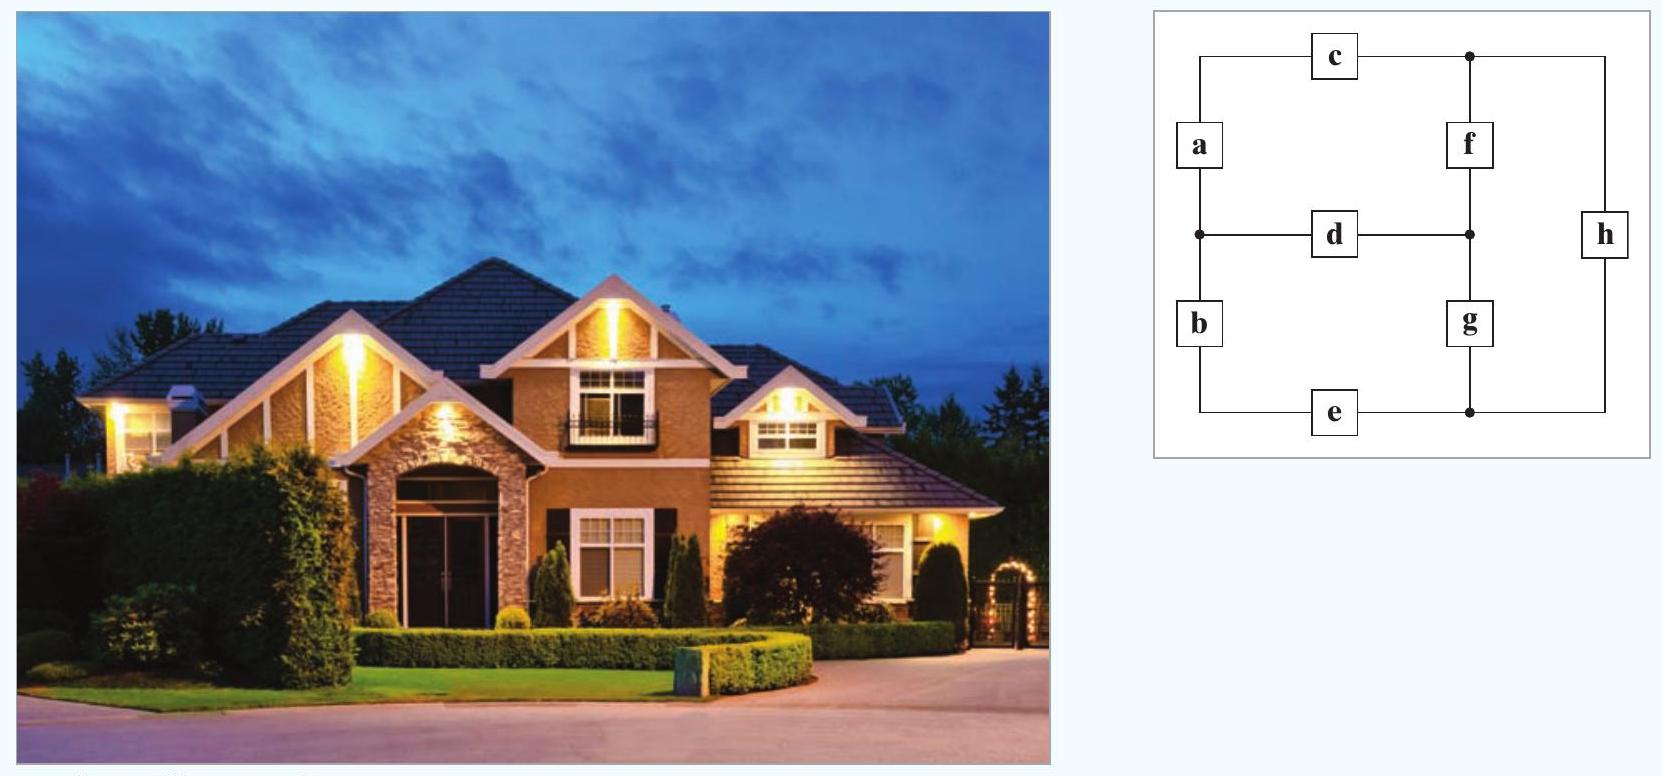
\includegraphics[max width=\textwidth, center]{2024_10_28_c0e2dc6a235cac59ec77g-027(1)}\\
romakoma / Shutterstock\\
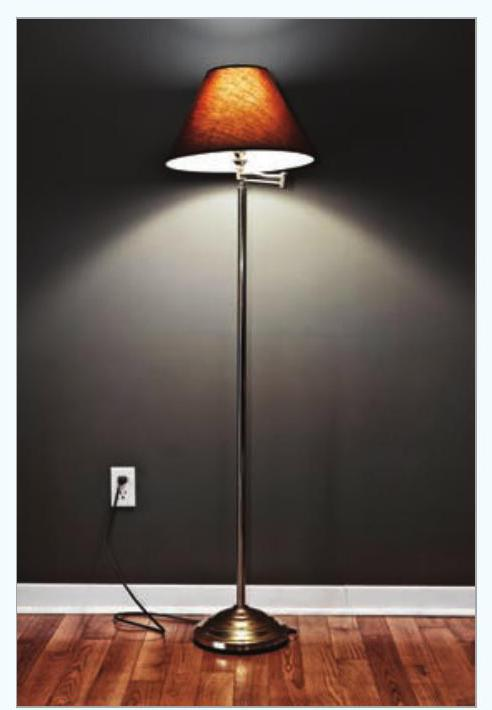
\includegraphics[max width=\textwidth, center]{2024_10_28_c0e2dc6a235cac59ec77g-027}

Elena Elisseeva /Alamy\\
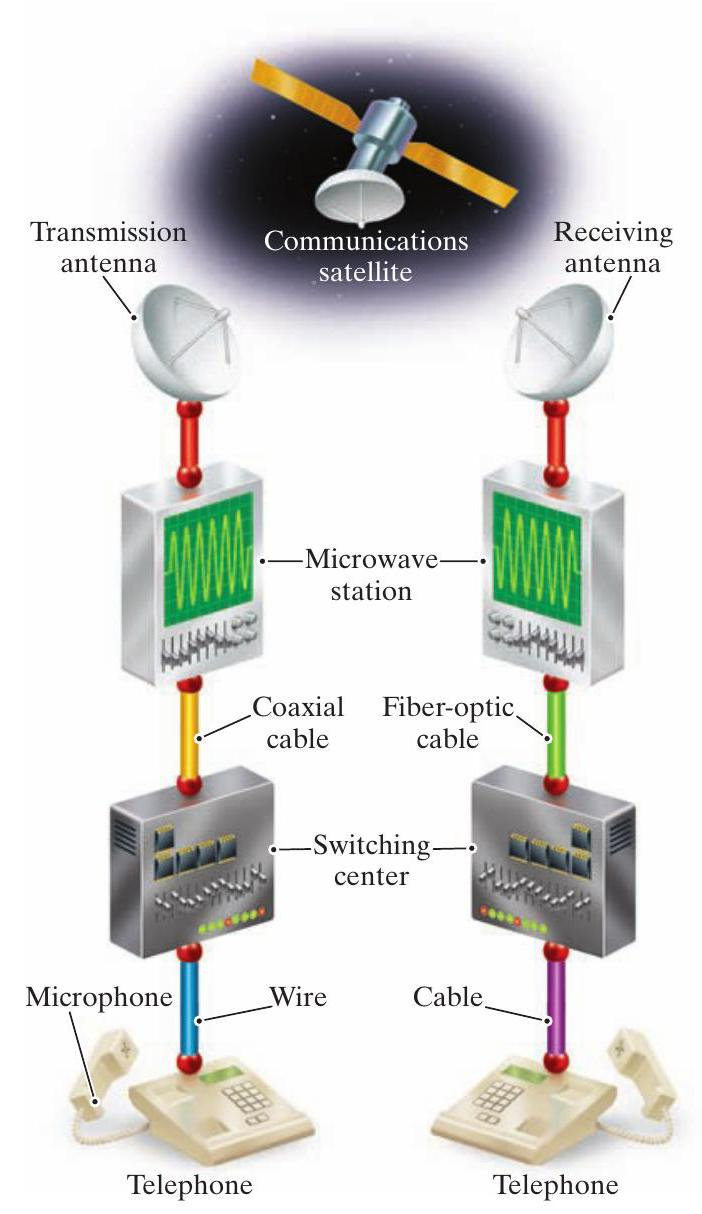
\includegraphics[max width=\textwidth, center]{2024_10_28_c0e2dc6a235cac59ec77g-028}

Figure 1.1 A A telephone system.

\subsection*{1.1 Electrical Engineering: An Overview}
Electrical engineering is the profession concerned with systems that produce, transmit, and measure electric signals. Electrical engineering combines the physicist's models of natural phenomena with the mathematician's tools for manipulating those models to produce systems that meet practical needs. Electrical systems pervade our lives; they are found in homes, schools, workplaces, and transportation vehicles everywhere. We begin by presenting a few examples from each of the five major classifications of electrical systems:

\begin{itemize}
  \item communication systems
  \item computer systems
  \item control systems
  \item power systems
  \item signal-processing systems
\end{itemize}

Then we describe how electrical engineers analyze and design such systems.\\
Communication systems are electrical systems that generate, transmit, and distribute information. Well-known examples include television equipment, such as cameras, transmitters, receivers, and VCRs; radio telescopes, used to explore the universe; satellite systems, which return images of other planets and our own; radar systems, used to coordinate plane flights; and telephone systems.

Figure 1.1 depicts the major components of a modern telephone system. Starting at the left of the figure, inside a telephone, a microphone turns sound waves into electric signals. These signals are carried to a switching center where they are combined with the signals from tens, hundreds, or thousands of other telephones. The combined signals leave the switching center; their form depends on the distance they must travel. In our example, they are sent through wires in underground coaxial cables to a microwave transmission station. Here, the signals are transformed into microwave frequencies and broadcast from a transmission antenna through air and space, via a communications satellite, to a receiving antenna. The microwave receiving station translates the microwave signals into a form suitable for further transmission, perhaps as pulses of light to be sent through fiber-optic cable. On arrival at the second switching center, the combined signals are separated, and each is routed to the appropriate telephone, where an earphone acts as a speaker to convert the received electric signals back into sound waves. At each stage of the process, electric circuits operate on the signals. Imagine the challenge involved in designing, building, and operating each circuit in a way that guarantees that all of the hundreds of thousands of simultaneous calls have high-quality connections.

Computer systems use electric signals to process information ranging from word processing to mathematical computations. Systems range in size and power from pocket calculators to personal computers to supercomputers that perform such complex tasks as processing weather data and modeling chemical interactions of complex organic molecules. These systems include networks of microcircuits, or integrated circuits-postage-stampsized assemblies of hundreds, thousands, or millions of electrical components that often operate at speeds and power levels close to fundamental physical limits, including the speed of light and the thermodynamic laws.

Control systems use electric signals to regulate processes. Examples include the control of temperatures, pressures, and flow rates in an oil refinery; the fuel-air mixture in a fuel-injected automobile engine; mechanisms such as the motors, doors, and lights in elevators; and the locks in the

Panama Canal. The autopilot and autolanding systems that help to fly and land airplanes are also familiar control systems.

Power systems generate and distribute electric power. Electric power, which is the foundation of our technology-based society, usually is generated in large quantities by nuclear, hydroelectric, and thermal (coal-, oil-, or gas-fired) generators. Power is distributed by a grid of conductors that crisscross the country. A major challenge in designing and operating such a system is to provide sufficient redundancy and control so that failure of any piece of equipment does not leave a city, state, or region completely without power.

Signal-processing systems act on electric signals that represent information. They transform the signals and the information contained in them into a more suitable form. There are many different ways to process the signals and their information. For example, image-processing systems gather massive quantities of data from orbiting weather satellites, reduce the amount of data to a manageable level, and transform the remaining data into a video image for the evening news broadcast. A computerized tomography (CT) scan is another example of an image-processing system. It takes signals generated by a special X-ray machine and transforms them into an image such as the one in Fig. 1.2. Although the original X-ray signals are of little use to a physician, once they are processed into a recognizable image the information they contain can be used in the diagnosis of disease and injury.

Considerable interaction takes place among the engineering disciplines involved in designing and operating these five classes of systems. Thus communications engineers use digital computers to control the flow of information. Computers contain control systems, and control systems contain computers. Power systems require extensive communications systems to coordinate safely and reliably the operation of components, which may be spread across a continent. A signal-processing system may involve a communications link, a computer, and a control system.

A good example of the interaction among systems is a commercial airplane, such as the one shown in Fig. 1.3. A sophisticated communications system enables the pilot and the air traffic controller to monitor the plane's location, permitting the air traffic controller to design a safe flight path for all of the nearby aircraft and enabling the pilot to keep the plane on its designated path. On the newest commercial airplanes, an onboard computer system is used for managing engine functions, implementing the navigation and flight control systems, and generating video information screens in the cockpit. A complex control system uses cockpit commands to adjust the position and speed of the airplane, producing the appropriate signals to the engines and the control surfaces (such as the wing flaps, ailerons, and rudder) to ensure the plane remains safely airborne and on the desired flight path. The plane must have its own power system to stay aloft and to provide and distribute the electric power needed to keep the cabin lights on, make the coffee, and show the movie. Signal-processing systems reduce the noise in air traffic communications and transform information about the plane's location into the more meaningful form of a video display in the cockpit. Engineering challenges abound in the design of each of these systems and their integration into a coherent whole. For example, these systems must operate in widely varying and unpredictable environmental conditions. Perhaps the most important engineering challenge is to guarantee that sufficient redundancy is incorporated in the designs to ensure that passengers arrive safely and on time at their desired destinations.

Although electrical engineers may be interested primarily in one area, they must also be knowledgeable in other areas that interact with this area of interest. This interaction is part of what makes electrical\\
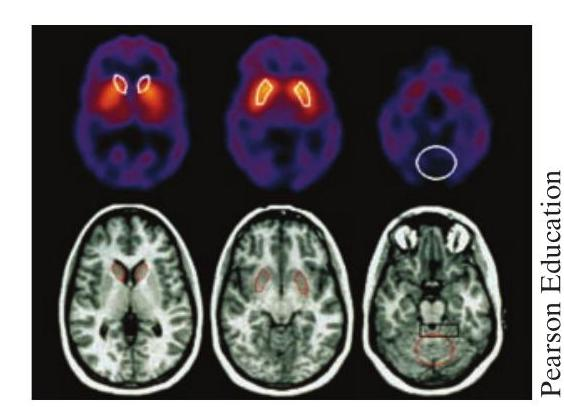
\includegraphics[max width=\textwidth, center]{2024_10_28_c0e2dc6a235cac59ec77g-029}

Figure 1.2 $\triangle$ A CT scan of an adult head.\\
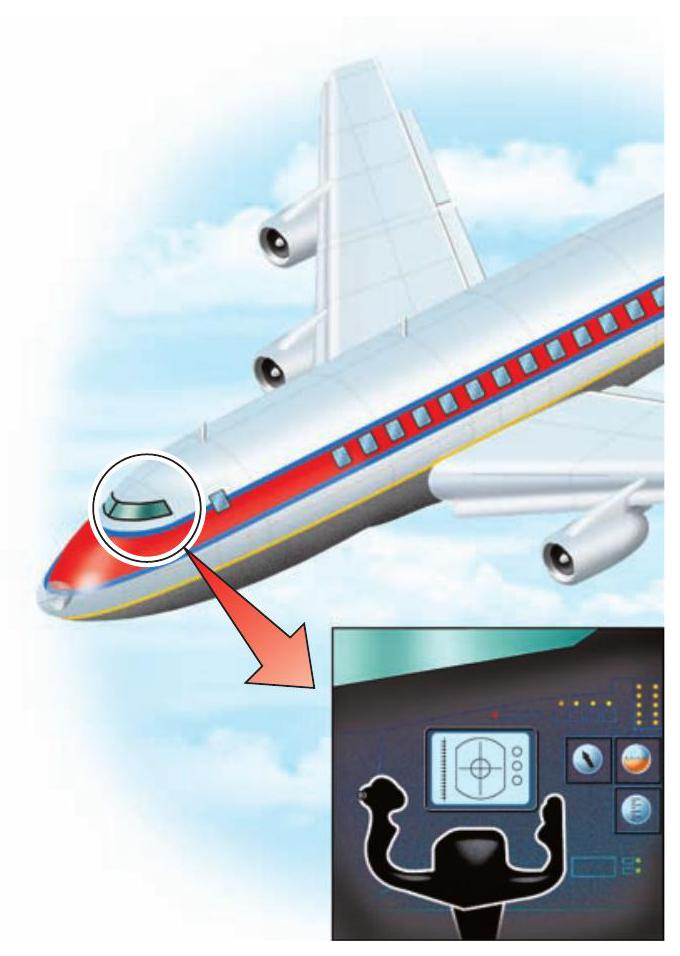
\includegraphics[max width=\textwidth, center]{2024_10_28_c0e2dc6a235cac59ec77g-029(1)}

Figure 1.3 A An airplane.\\
engineering a challenging and exciting profession. The emphasis in engineering is on making things work, so an engineer is free to acquire and use any technique, from any field, that helps to get the job done.

\section*{Circuit Theory}
In a field as diverse as electrical engineering, you might well ask whether all of its branches have anything in common. The answer is yes-electric circuits. An electric circuit is a mathematical model that approximates the behavior of an actual electrical system. As such, it provides an important foundation for learning-in your later courses and as a practicing engineer-the details of how to design and operate systems such as those just described. The models, the mathematical techniques, and the language of circuit theory will form the intellectual framework for your future engineering endeavors.

Note that the term electric circuit is commonly used to refer to an actual electrical system as well as to the model that represents it. In this text, when we talk about an electric circuit, we always mean a model, unless otherwise stated. It is the modeling aspect of circuit theory that has broad applications across engineering disciplines.

Circuit theory is a special case of electromagnetic field theory: the study of static and moving electric charges. Although generalized field theory might seem to be an appropriate starting point for investigating electric signals, its application is not only cumbersome but also requires the use of advanced mathematics. Consequently, a course in electromagnetic field theory is not a prerequisite to understanding the material in this book. We do, however, assume that you have had an introductory physics course in which electrical and magnetic phenomena were discussed.

Three basic assumptions permit us to use circuit theory, rather than electromagnetic field theory, to study a physical system represented by an electric circuit. These assumptions are as follows:

\begin{enumerate}
  \item Electrical effects happen instantaneously throughout a system. We can make this assumption because we know that electric signals travel at or near the speed of light. Thus, if the system is physically small, electric signals move through it so quickly that we can consider them to affect every point in the system simultaneously. A system that is small enough so that we can make this assumption is called a lumped-parameter system.
  \item The net charge on every component in the system is always zero. Thus no component can collect a net excess of charge, although some components, as you will learn later, can hold equal but opposite separated charges.
  \item There is no magnetic coupling between the components in a system. As we demonstrate later, magnetic coupling can occur within a component.\\
That's it; there are no other assumptions. Using circuit theory provides simple solutions (of sufficient accuracy) to problems that would become hopelessly complicated if we were to use electromagnetic field theory. These benefits are so great that engineers sometimes specifically design electrical systems to ensure that these assumptions are met. The importance of assumptions 2 and 3 becomes apparent after we introduce the basic circuit elements and the rules for analyzing interconnected elements.
\end{enumerate}

However, we need to take a closer look at assumption 1. The question is, "How small does a physical system have to be to qualify as a lumpedparameter system?" We can get a quantitative handle on the question by noting that electric signals propagate by wave phenomena. If the wavelength of the signal is large compared to the physical dimensions of the\\
system, we have a lumped-parameter system. The wavelength $\lambda$ is the velocity divided by the repetition rate, or frequency, of the signal; that is, $\lambda=c / f$. The frequency $f$ is measured in hertz $(\mathrm{Hz})$. For example, power systems in the United States operate at 60 Hz . If we use the speed of light $\left(c=3 \times 10^{8} \mathrm{~m} / \mathrm{s}\right)$ as the velocity of propagation, the wavelength is $5 \times 10^{6} \mathrm{~m}$. If the power system of interest is physically smaller than this wavelength, we can represent it as a lumped-parameter system and use circuit theory to analyze its behavior. How do we define smaller? A good rule is the rule of $1 / 10$ th: If the dimension of the system is $1 / 10$ th (or smaller) of the dimension of the wavelength, you have a lumped-parameter system. Thus, as long as the physical dimension of the power system is less than $5 \times 10^{5} \mathrm{~m}$, we can treat it as a lumped-parameter system.

On the other hand, the propagation frequency of radio signals is on the order of $10^{9} \mathrm{~Hz}$. Thus the wavelength is 0.3 m . Using the rule of $1 / 10$ th, the relevant dimensions of a communication system that sends or receives radio signals must be less than 3 cm to qualify as a lumped-parameter system. Whenever any of the pertinent physical dimensions of a system under study approaches the wavelength of its signals, we must use electromagnetic field theory to analyze that system. Throughout this book we study circuits derived from lumped-parameter systems.

\section*{Problem Solving}
As a practicing engineer, you will not be asked to solve problems that have already been solved. Whether you are trying to improve the performance of an existing system or creating a new system, you will be working on unsolved problems. As a student, however, you will devote much of your attention to the discussion of problems already solved. By reading about and discussing how these problems were solved in the past, and by solving related homework and exam problems on your own, you will begin to develop the skills to successfully attack the unsolved problems you'll face as a practicing engineer.

Some general problem-solving procedures are presented here. Many of them pertain to thinking about and organizing your solution strategy before proceeding with calculations.

\begin{enumerate}
  \item Identify what's given and what's to be found. In problem solving, you need to know your destination before you can select a route for getting there. What is the problem asking you to solve or find? Sometimes the goal of the problem is obvious; other times you may need to paraphrase or make lists or tables of known and unknown information to see your objective.
\end{enumerate}

The problem statement may contain extraneous information that you need to weed out before proceeding. On the other hand, it may offer incomplete information or more complexities than can be handled given the solution methods at your disposal. In that case, you'll need to make assumptions to fill in the missing information or simplify the problem context. Be prepared to circle back and reconsider supposedly extraneous information and/or your assumptions if your calculations get bogged down or produce an answer that doesn't seem to make sense.\\
2. Sketch a circuit diagram or other visual model. Translating a verbal problem description into a visual model is often a useful step in the solution process. If a circuit diagram is already provided, you may need to add information to it, such as labels, values, or reference directions. You may also want to redraw the circuit in a simpler, but equivalent, form. Later in this text you will learn the methods for developing such simplified equivalent circuits.\\
3. Think of several solution methods and decide on a way of choosing among them. This course will help you build a collection of analytical tools, several of which may work on a given problem. But one method may produce fewer equations to be solved than another, or it may require only algebra instead of calculus to reach a solution. Such efficiencies, if you can anticipate them, can streamline your calculations considerably. Having an alternative method in mind also gives you a path to pursue if your first solution attempt bogs down.\\
4. Calculate a solution. Your planning up to this point should have helped you identify a good analytical method and the correct equations for the problem. Now comes the solution of those equations. Paper-and-pencil, calculator, and computer methods are all available for performing the actual calculations of circuit analysis. Efficiency and your instructor's preferences will dictate which tools you should use.\\
5. Use your creativity. If you suspect that your answer is off base or if the calculations seem to go on and on without moving you toward a solution, you should pause and consider alternatives. You may need to revisit your assumptions or select a different solution method. Or, you may need to take a less-conventional problem-solving approach, such as working backward from a solution. This text provides answers to all of the Assessment Problems and many of the Chapter Problems so that you may work backward when you get stuck. In the real world, you won't be given answers in advance, but you may have a desired problem outcome in mind from which you can work backward. Other creative approaches include allowing yourself to see parallels with other types of problems you've successfully solved, following your intuition or hunches about how to proceed, and simply setting the problem aside temporarily and coming back to it later.\\
6. Test your solution. Ask yourself whether the solution you've obtained makes sense. Does the magnitude of the answer seem reasonable? Is the solution physically realizable? You may want to go further and rework the problem via an alternative method. Doing so will not only test the validity of your original answer, but will also help you develop your intuition about the most efficient solution methods for various kinds of problems. In the real world, safetycritical designs are always checked by several independent means. Getting into the habit of checking your answers will benefit you as a student and as a practicing engineer.

These problem-solving steps cannot be used as a recipe to solve every problem in this or any other course. You may need to skip, change the order of, or elaborate on certain steps to solve a particular problem. Use these steps as a guideline to develop a problem-solving style that works for you.

\subsection*{1.2 The International System of Units}
Engineers compare theoretical results to experimental results and compare competing engineering designs using quantitative measures. Modern engineering is a multidisciplinary profession in which teams of engineers work together on projects, and they can communicate their results in a meaningful way only if they all use the same units of measure. The International System of Units (abbreviated SI) is used by all the major engineering societies and most engineers throughout the world; hence we use it in this book.

TABLE 1.1 The International System of Units (SI)

\begin{center}
\begin{tabular}{lll}
Quantity & Basic Unit & Symbol \\
\hline
Length & meter & m \\
Mass & kilogram & kg \\
Time & second & s \\
Electric current & ampere & A \\
Thermodynamic temperature & degree kelvin & K \\
Amount of substance & mole & mol \\
Luminous intensity & candela & cd \\
\hline
\end{tabular}
\end{center}

National Institute of Standards and Technology Special Publication 330, 2008 Edition, Natl. Inst. Stand. Technol. Spec. Pub. 330, 2008 Ed., 96 pages (March 2008)

The SI units are based on seven defined quantities:

\begin{itemize}
  \item length
  \item mass
  \item time
  \item electric current
  \item thermodynamic temperature
  \item amount of substance
  \item luminous intensity
\end{itemize}

These quantities, along with the basic unit and symbol for each, are listed in Table 1.1. Although not strictly SI units, the familiar time units of minute ( 60 s ), hour ( 3600 s ), and so on are often used in engineering calculations. In addition, defined quantities are combined to form derived units. Some, such as force, energy, power, and electric charge, you already know through previous physics courses. Table 1.2 lists the derived units used in this book.

In many cases, the SI unit is either too small or too large to use conveniently. Standard prefixes corresponding to powers of 10 , as listed in Table 1.3, are then applied to the basic unit. All of these prefixes are correct, but engineers often use only the ones for powers divisible by 3 ; thus centi, deci, deka, and hecto are used rarely. Also, engineers often select the prefix that places the base number in the range between 1 and 1000. Suppose that a time calculation yields a result of $10^{-5} \mathrm{~s}$, that is, 0.00001 s . Most engineers would describe this quantity as $10 \mu \mathrm{~s}$, that is, $10^{-5}=10 \times 10^{-6} \mathrm{~s}$, rather than as 0.01 ms or $10,000,000 \mathrm{ps}$.

TABLE 1.2 Derived Units in SI

\begin{center}
\begin{tabular}{lll}
Quantity & Unit Name (Symbol) & Formula \\
\hline
Frequency & hertz $(\mathrm{Hz})$ & $\mathrm{s}^{-1}$ \\
Force & newton $(\mathrm{N})$ & $\mathrm{kg} \cdot \mathrm{m} / \mathrm{s}^{2}$ \\
Energy or work & joule $(\mathrm{J})$ & $\mathrm{N} \cdot \mathrm{m}$ \\
Power & watt $(\mathrm{W})$ & $\mathrm{J} / \mathrm{s}$ \\
Electric charge & $\operatorname{coulomb}(\mathrm{C})$ & $\mathrm{A} \cdot \mathrm{s}$ \\
Electric potential & $\operatorname{volt}(\mathrm{V})$ & $\mathrm{J} / \mathrm{C}$ \\
Electric resistance & ohm $(\Omega)$ & $\mathrm{V} / \mathrm{A}$ \\
Electric conductance & $\operatorname{siemens}(\mathrm{S})$ & $\mathrm{A} / \mathrm{V}$ \\
Electric capacitance & farad $(\mathrm{F})$ & $\mathrm{C} / \mathrm{V}$ \\
Magnetic flux & weber $(\mathrm{Wb})$ & $\mathrm{V} \cdot \mathrm{s}$ \\
Inductance & henry $(\mathrm{H})$ & $\mathrm{Wb} / \mathrm{A}$ \\
\hline
\end{tabular}
\end{center}

National Institute of Standards and Technology Special Publication 330, 2008 Edition, Natl. Inst. Stand. Technol. Spec. Pub. 330, 2008 Ed., 96 pages (March 2008)

TABLE 1.3 Standardized Prefixes to Signify Powers of 10

\begin{center}
\begin{tabular}{lll}
Prefix & Symbol & Power \\
atto & a & $10^{-18}$ \\
femto & f & $10^{-15}$ \\
pico & p & $10^{-12}$ \\
nano & n & $10^{-9}$ \\
micro & $\mu$ & $10^{-6}$ \\
milli & m & $10^{-3}$ \\
centi & c & $10^{-2}$ \\
deci & d & $10^{-1}$ \\
deka & da & 10 \\
hecto & h & $10^{2}$ \\
kilo & k & $10^{3}$ \\
mega & M & $10^{6}$ \\
giga & G & $10^{9}$ \\
tera & T & $10^{12}$ \\
\hline
\end{tabular}
\end{center}

National Institute of Standards and Technology Special Publication 330, 2008 Edition, Natl. Inst. Stand. Technol. Spec. Pub. 330, 2008 Ed., 96 pages (March 2008)

Example 1.1 illustrates a method for converting from one set of units to another and also uses power-of-ten prefixes.

\section*{Example 1.1 Using SI Units and Prefixes for Powers of 10}
If a signal can travel in a cable at $80 \%$ of the speed of light, what length of cable, in inches, represents 1 ns ?

Therefore, a signal traveling at $80 \%$ of the speed of light will cover 9.45 inches of cable in 1 nanosecond.

\section*{Solution}
First, note that $1 \mathrm{~ns}=10^{-9} \mathrm{~s}$. Also, recall that the speed of light $c=3 \times 10^{8} \mathrm{~m} / \mathrm{s}$. Then, $80 \%$ of the speed of light is $0.8 c=(0.8)\left(3 \times 10^{8}\right)=$ $2.4 \times 10^{8} \mathrm{~m} / \mathrm{s}$. Using a product of ratios, we can convert $80 \%$ of the speed of light from meters-persecond to inches-per-nanosecond. The result is the distance in inches traveled in 1 ns :

$$
\begin{aligned}
& \frac{2.4 \times 10^{8} \text { meters }}{1 \text { second }} \cdot \frac{1 \text { second }}{10^{9} \text { nanoseconds }} \cdot \frac{100 \text { centimeters }}{1 \text { meter }} \cdot \frac{1 \text { inch }}{2.54 \text { centimeters }} \\
& =\frac{\left(2.4 \times 10^{8}\right)(100)}{\left(10^{9}\right)(2.54)}=9.45 \text { inches } / \text { nanosecond }
\end{aligned}
$$

\section*{ASSESSMENT PROBLEMS}
Objective 1-Understand and be able to use SI units and the standard prefixes for powers of 10\\
1.1 Assume a telephone signal travels through a cable at two-thirds the speed of light. How long does it take the signal to get from New York City to Miami if the distance is approximately 1100 miles?

Answer: 8.85 ms .\\
NOTE: Also try Chapter Problems 1.1, 1.3, and 1.5.\\
1.2 How many dollars per millisecond would the federal government have to collect to retire a deficit of $\$ 100$ billion in one year?\\
Answer: \$3.17/ms.

\subsection*{1.3 Circuit Analysis: An Overview}
Before becoming involved in the details of circuit analysis, we need to take a broad look at engineering design, specifically the design of electric circuits. The purpose of this overview is to provide you with a perspective on where circuit analysis fits within the whole of circuit design. Even though this book focuses on circuit analysis, we try to provide opportunities for circuit design where appropriate.

All engineering designs begin with a need, as shown in Fig. 1.4. This need may come from the desire to improve on an existing design, or it may be something brand-new. A careful assessment of the need results in design specifications, which are measurable characteristics of a proposed design. Once a design is proposed, the design specifications allow us to assess whether or not the design actually meets the need.

A concept for the design comes next. The concept derives from a complete understanding of the design specifications coupled with an insight into\\
the need, which comes from education and experience. The concept may be realized as a sketch, as a written description, or in some other form. Often the next step is to translate the concept into a mathematical model. A commonly used mathematical model for electrical systems is a circuit model.

The elements that comprise the circuit model are called ideal circuit components. An ideal circuit component is a mathematical model of an actual electrical component, like a battery or a light bulb. It is important for the ideal circuit component used in a circuit model to represent the behavior of the actual electrical component to an acceptable degree of accuracy. The tools of circuit analysis, the focus of this book, are then applied to the circuit. Circuit analysis is based on mathematical techniques and is used to predict the behavior of the circuit model and its ideal circuit components. A comparison between the desired behavior, from the design specifications, and the predicted behavior, from circuit analysis, may lead to refinements in the circuit model and its ideal circuit elements. Once the desired and predicted behavior are in agreement, a physical prototype can be constructed.

The physical prototype is an actual electrical system, constructed from actual electrical components. Measurement techniques are used to determine the actual, quantitative behavior of the physical system. This actual behavior is compared with the desired behavior from the design specifications and the predicted behavior from circuit analysis. The comparisons may result in refinements to the physical prototype, the circuit model, or both. Eventually, this iterative process, in which models, components, and systems are continually refined, may produce a design that accurately matches the design specifications and thus meets the need.

From this description, it is clear that circuit analysis plays a very important role in the design process. Because circuit analysis is applied to circuit models, practicing engineers try to use mature circuit models so that the resulting designs will meet the design specifications in the first iteration. In this book, we use models that have been tested for between 20 and 100 years; you can assume that they are mature. The ability to model actual electrical systems with ideal circuit elements makes circuit theory extremely useful to engineers.

Saying that the interconnection of ideal circuit elements can be used to quantitatively predict the behavior of a system implies that we can describe the interconnection with mathematical equations. For the mathematical equations to be useful, we must write them in terms of measurable quantities. In the case of circuits, these quantities are voltage and current, which we discuss in Section 1.4. The study of circuit analysis involves understanding the behavior of each ideal circuit element in terms of its voltage and current and understanding the constraints imposed on the voltage and current as a result of interconnecting the ideal elements.

\subsection*{1.4 Voltage and Current}
The concept of electric charge is the basis for describing all electrical phenomena. Let's review some important characteristics of electric charge.

\begin{itemize}
  \item The charge is bipolar, meaning that electrical effects are described in terms of positive and negative charges.
  \item The electric charge exists in discrete quantities, which are integral multiples of the electronic charge, $1.6022 \times 10^{-19} \mathrm{C}$.
  \item Electrical effects are attributed to both the separation of charge and charges in motion.
\end{itemize}

In circuit theory, the separation of charge creates an electric force (voltage), and the motion of charge creates an electric fluid (current).\\
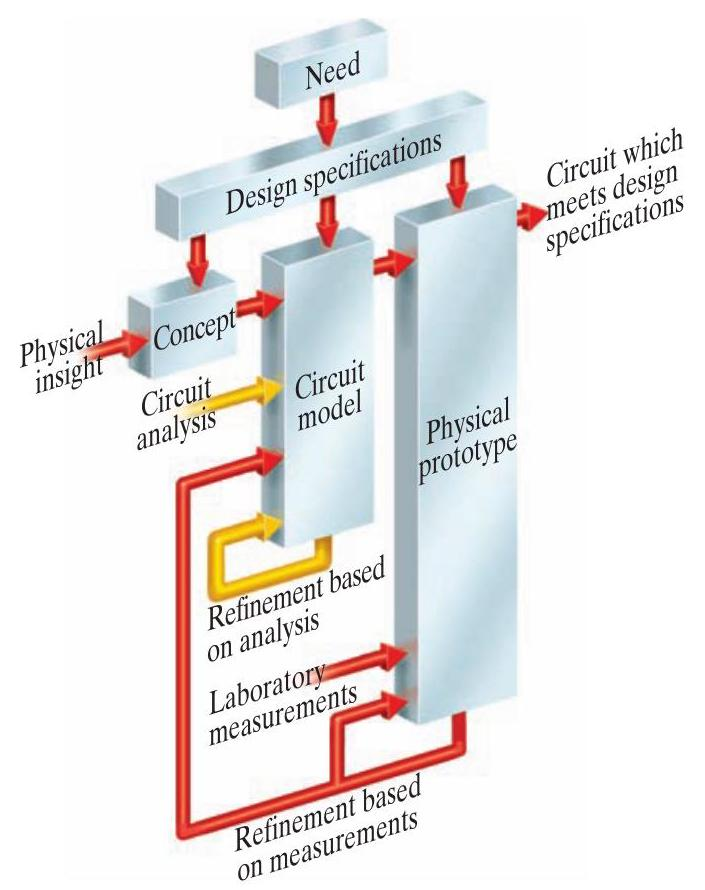
\includegraphics[max width=\textwidth, center]{2024_10_28_c0e2dc6a235cac59ec77g-035}

Figure $1.4 \triangle$ A conceptual model for electrical engineering design.

\section*{Definition of voltage}
\section*{Definition of current $\downarrow$}
The concepts of voltage and current are useful from an engineering point of view because they can be expressed quantitatively. Whenever positive and negative charges are separated, energy is expended. Voltage is the energy per unit charge created by the separation. We express this ratio in differential form as


\begin{equation*}
v=\frac{d w}{d q} \tag{1.1}
\end{equation*}


where\\
$v=$ the voltage in volts,\\
$w=$ the energy in joules,\\
$q=$ the charge in coulombs.\\
The electrical effects caused by charges in motion depend on the rate of charge flow. The rate of charge flow is known as the electric current, which is expressed as


\begin{equation*}
i=\frac{d q}{d t} \tag{1.2}
\end{equation*}


where\\
$i=$ the current in amperes,\\
$q=$ the charge in coulombs,\\
$t=$ the time in seconds.\\
Equations 1.1 and 1.2 are definitions for the magnitude of voltage and current, respectively. The bipolar nature of electric charge requires that we assign polarity references to these variables. We will do so in Section 1.5.

Although current is made up of discrete, moving electrons, we do not need to consider them individually because of the enormous number of them. Rather, we can think of electrons and their corresponding charge as one smoothly flowing entity. Thus, $i$ is treated as a continuous variable.

One advantage of using circuit models is that we can model a component strictly in terms of the voltage and current at its terminals. Thus two physically different components could have the same relationship between the terminal voltage and terminal current. If they do, for purposes of circuit analysis, they are identical. Once we know how a component behaves at its terminals, we can analyze its behavior in a circuit. However, when developing circuit models, we are interested in a component's internal behavior. We might want to know, for example, whether charge conduction is taking place because of free electrons moving through the crystal lattice structure of a metal or whether it is because of electrons moving within the covalent bonds of a semiconductor material. However, these concerns are beyond the realm of circuit theory. In this book we use circuit models that have already been developed; we do not discuss how component models are developed.

\subsection*{1.5 The Ideal Basic Circuit Element}
An ideal basic circuit element has three attributes: (1) it has only two terminals, which are points of connection to other circuit components; (2) it is described mathematically in terms of current and/or voltage; and (3) it cannot be subdivided into other elements. We use the word ideal to imply\\
that a basic circuit element does not exist as a realizable physical component. However, as we discussed in Section 1.3, ideal elements can be connected in order to model actual devices and systems. We use the word basic to imply that the circuit element cannot be further reduced or subdivided into other elements. Thus the basic circuit elements form the building blocks for constructing circuit models, but they themselves cannot be modeled with any other type of element.

Figure 1.5 is a representation of an ideal basic circuit element. The box is blank because we are making no commitment at this time as to the type of circuit element it is. In Fig. 1.5, the voltage across the terminals of the box is denoted by $v$, and the current in the circuit element is denoted by $i$. The polarity reference for the voltage is indicated by the plus and minus signs, and the reference direction for the current is shown by the arrow placed alongside the current. The interpretation of these references given positive or negative numerical values of $v$ and $i$ is summarized in Table 1.4. Note that algebraically the notion of positive charge flowing in one direction is equivalent to the notion of negative charge flowing in the opposite direction.

The assignments of the reference polarity for voltage and the reference direction for current are entirely arbitrary. However, once you have assigned the references, you must write all subsequent equations to agree with the chosen references. The most widely used sign convention applied to these references is called the passive sign convention, which we use throughout this book. The passive sign convention can be stated as follows:

Whenever the reference direction for the current in an element is in the direction of the reference voltage drop across the element (as in Fig. 1.5), use a positive sign in any expression that relates the voltage to the current. Otherwise, use a negative sign.

We apply this sign convention in all the analyses that follow. Our purpose for introducing it even before we have introduced the different types of basic circuit elements is to impress on you the fact that the selection of polarity references along with the adoption of the passive sign convention is not a function of the basic elements nor the type of interconnections made with the basic elements. We present the application and interpretation of the passive sign convention in power calculations in Section 1.6.

Example 1.2 illustrates one use of the equation defining current.

TABLE 1.4 Interpretation of Reference Directions in Fig. 1.5

\section*{Positive Value}
$v$ voltage drop from terminal 1 to terminal 2\\
or\\
voltage rise from terminal 2 to terminal 1\\
$i$ positive charge flowing from terminal 1 to terminal 2 or\\
negative charge flowing from terminal 2 to terminal 1

Negative Value\\
voltage rise from terminal 1 to terminal 2\\
or\\
voltage drop from terminal 2 to terminal 1\\
positive charge flowing from terminal 2 to terminal 1\\
or\\
negative charge flowing from terminal 1 to terminal 2

\section*{Example 1.2 Relating Current and Charge}
No charge exists at the upper terminal of the element in Fig. 1.5 for $t<0$. At $t=0$, a 5 A current begins to flow into the upper terminal.\\
a) Derive the expression for the charge accumulating at the upper terminal of the element for $t>0$.\\
b) If the current is stopped after 10 seconds, how much charge has accumulated at the upper terminal?

\section*{Solution}
a) From the definition of current given in Eq. 1.2, the expression for charge accumulation due to current flow is

$$
q(t)=\int_{0}^{t} i(x) d x
$$

Therefore,

$$
q(t)=\int_{0}^{t} 5 d x=\left.5 x\right|_{0} ^{t}=5 t-5(0)=5 t \mathrm{C} \quad \text { for } t>0
$$

b) The total charge that accumulates at the upper terminal in 10 seconds due to a 5 A current is $q(10)=5(10)=50 \mathrm{C}$.

\section*{ASSESSMENT PROBLEMS}
\section*{Objective 2—Know and be able to use the definitions of voltage and current}
1.3 The current at the terminals of the element in Fig. 1.5 is

$$
\begin{array}{ll}
i=0, & t<0 \\
i=20 e^{-5000 t} \mathrm{~A}, & t \geq 0
\end{array}
$$

Calculate the total charge (in microcoulombs) entering the element at its upper terminal.

Answer: $4000 \mu \mathrm{C}$.\\
NOTE: Also try Chapter Problem 1.8.\\
1.4 The expression for the charge entering the upper terminal of Fig. 1.5 is

$$
q=\frac{1}{\alpha^{2}}-\left(\frac{t}{\alpha}+\frac{1}{\alpha^{2}}\right) e^{-\alpha t} \mathrm{C}
$$

Find the maximum value of the current entering the terminal if $\alpha=0.03679 \mathrm{~s}^{-1}$.

Answer: 10 A .

\subsection*{1.6 Power and Energy}
Power and energy calculations also are important in circuit analysis. One reason is that although voltage and current are useful variables in the analysis and design of electrically based systems, the useful output of the system often is nonelectrical, and this output is conveniently expressed in terms of power or energy. Another reason is that all practical devices have limitations on the amount of power that they can handle. In the design process, therefore, voltage and current calculations by themselves are not sufficient.

We now relate power and energy to voltage and current and at the same time use the power calculation to illustrate the passive sign convention. Recall from basic physics that power is the time rate of expending or\\
absorbing energy. (A water pump rated 75 kW can deliver more liters per second than one rated 7.5 kW .) Mathematically, energy per unit time is expressed in the form of a derivative, or


\begin{equation*}
p=\frac{d w}{d t} \tag{1.3}
\end{equation*}


where

$$
\begin{aligned}
p & =\text { the power in watts } \\
w & =\text { the energy in joules } \\
i & =\text { the time in seconds. }
\end{aligned}
$$

Thus 1 W is equivalent to $1 \mathrm{~J} / \mathrm{s}$.\\
The power associated with the flow of charge follows directly from the definition of voltage and current in Eqs. 1.1 and 1.2, or

$$
p=\frac{d w}{d t}=\left(\frac{d w}{d q}\right)\left(\frac{d q}{d t}\right)
$$

SO


\begin{equation*}
p=v i \tag{1.4}
\end{equation*}


where

$$
\begin{aligned}
p & =\text { the power in watts, } \\
v & =\text { the voltage in volts, } \\
i & =\text { the current in amperes. }
\end{aligned}
$$

Equation 1.4 shows that the power associated with a basic circuit element is simply the product of the current in the element and the voltage across the element. Therefore, power is a quantity associated with a pair of terminals, and we have to be able to tell from our calculation whether power is being delivered to the pair of terminals or extracted from it. This information comes from the correct application and interpretation of the passive sign convention.

If we use the passive sign convention, Eq. 1.4 is correct if the reference direction for the current is in the direction of the reference voltage drop across the terminals. Otherwise, Eq. 1.4 must be written with a minus sign. In other words, if the current reference is in the direction of a reference voltage rise across the terminals, the expression for the power is


\begin{equation*}
p=-v i \tag{1.5}
\end{equation*}


The algebraic sign of power is based on charge movement through voltage drops and rises. As positive charges move through a drop in voltage, they lose energy, and as they move through a rise in voltage, they gain energy. Figure 1.6 summarizes the relationship between the polarity references for voltage and current and the expression for power.\\
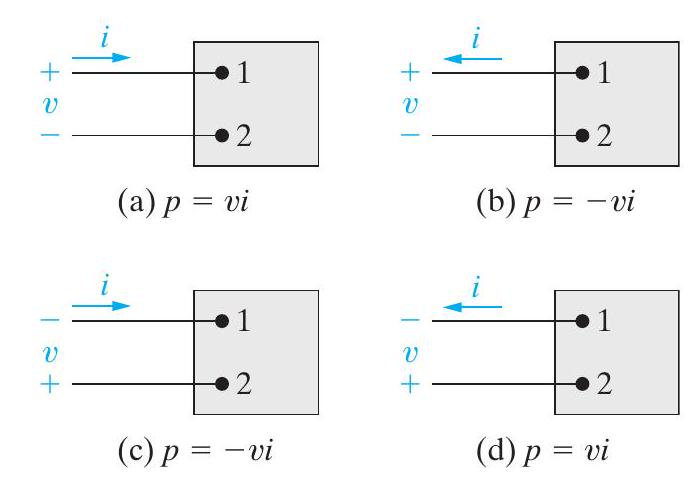
\includegraphics[max width=\textwidth, center]{2024_10_28_c0e2dc6a235cac59ec77g-039}

Figure 1.6 $\boldsymbol{\Delta}$ Polarity references and the expression for power.

We can now state the rule for interpreting the algebraic sign of power:

If the power is positive (that is, if $p>0$ ), power is being delivered to the circuit inside the box. If the power is negative (that is, if $p<0$ ), power is being extracted from the circuit inside the box.

For example, suppose that we have selected the polarity references shown in Fig. 1.6(b). Assume further that our calculations for the current and voltage yield the following numerical results:

$$
i=4 \mathrm{~A} \quad \text { and } \quad v=-10 \mathrm{~V}
$$

Then the power associated with the terminal pair 1,2 is

$$
p=-(-10)(4)=40 \mathrm{~W}
$$

Thus the circuit inside the box is absorbing 40 W .\\
To take this analysis one step further, assume that a colleague is solving the same problem but has chosen the reference polarities shown in Fig. 1.6(c). The resulting numerical values are

$$
i=-4 \mathrm{~A}, \quad v=10 \mathrm{~V}, \quad \text { and } \quad p=40 \mathrm{~W}
$$

Note that interpreting these results in terms of this reference system gives the same conclusions that we previously obtained-namely, that the circuit inside the box is absorbing 40 W . In fact, any of the reference systems in Fig. 1.6 yields this same result.

Example 1.3 illustrates the relationship between voltage, current, power, and energy for an ideal basic circuit element and the use of the passive sign convention.

\section*{Example 1.3 Relating Voltage, Current, Power, and Energy}
Assume that the voltage at the terminals of the element in Fig. 1.5, whose current was defined in Assessment Problem 1.3, is

$$
\begin{array}{ll}
v=0 & t<0 \\
v=10 e^{-5000 t} \mathrm{kV}, & t \geq 0
\end{array}
$$

a) Calculate the power supplied to the element at 1 ms .\\
b) Calculate the total energy (in joules) delivered to the circuit element.

\section*{Solution}
a) Since the current is entering the + terminal of the voltage drop defined for the element in Fig. 1.5, we use a " + " sign in the power equation.

$$
\begin{aligned}
& p=v i=\left(10,000 e^{-5000 t}\right)\left(20 e^{-5000 t}\right)=200,000 e^{-10,000 t} \mathrm{~W} \\
& \begin{aligned}
p(0.001) & =200,000 e^{-10,000 t(0.001)}=200,000 e^{-10} \\
& =200,000\left(45.4 \times 10^{-6}\right)=0.908 \mathrm{~W}
\end{aligned}
\end{aligned}
$$

b) From the definition of power given in Eq. 1.3, the expression for energy is

$$
w(t)=\int_{0}^{t} p(x) d x
$$

To find the total energy delivered, integrate the expresssion for power from zero to infinity. Therefore,

$$
\begin{aligned}
w_{\text {total }}= & \int_{0}^{\infty} 200,000 e^{-10,000 x} d x=\left.\frac{200,000 e^{-10,000 x}}{-10,000}\right|_{0} ^{\infty} \\
& =-20 e^{-\infty}-\left(-20 e^{-0}\right)=0+20=20 \mathrm{~J}
\end{aligned}
$$

Thus, the total energy supplied to the circuit element is 20 J .

\section*{ASSESSMENT PROBLEMS}
Objective 3-Know and use the definitions of power and energy; Objective 4-Be able to use the passive sign convention\\
1.5 Assume that a 20 V voltage drop occurs across an element from terminal 2 to terminal 1 and that a current of 4 A enters terminal 2.\\
a) Specify the values of $v$ and $i$ for the polarity references shown in Fig. 1.6(a)-(d).\\
b) State whether the circuit inside the box is absorbing or delivering power.\\
c) How much power is the circuit absorbing?

Answer: (a) Circuit 1.6(a): $v=-20 \mathrm{~V}, i=-4 \mathrm{~A}$; circuit 1.6(b): $v=-20 \mathrm{~V}, i=4 \mathrm{~A}$; circuit 1.6(c): $v=20 \mathrm{~V}, i=-4 \mathrm{~A}$; circuit 1.6 (d): $v=20 \mathrm{~V}, i=4 \mathrm{~A}$;\\
(b) absorbing;\\
(c) 80 W .\\
1.6 The voltage and current at the terminals of the circuit element in Fig 1.5 are zero for $t<0$. For $t \geq 0$, they are

$$
\begin{aligned}
v & =80,000 t e^{-500 t} \mathrm{~V}, & & t \geq 0 \\
i & =15 t e^{-500 t} \mathrm{~A}, & & t \geq 0 .
\end{aligned}
$$

a) Find the time when the power delivered to the circuit element is maximum.\\
b) Find the maximum value of power.\\
c) Find the total energy delivered to the circuit element.

Answer: (a) 2 ms ; (b) 649.6 mW ; (c) 2.4 mJ .\\
1.7 A high-voltage direct-current (dc) transmission line between Celilo, Oregon and Sylmar, California is operating at 800 kV and carrying 1800 A, as shown. Calculate the power (in megawatts) at the Oregon end of the line and state the direction of power flow.\\
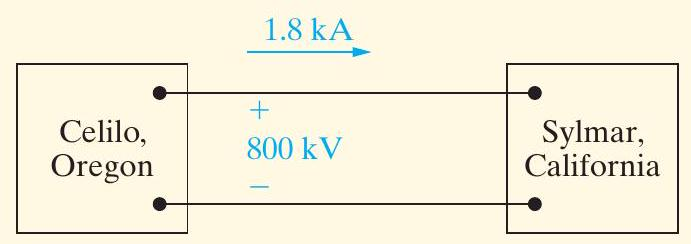
\includegraphics[max width=\textwidth, center]{2024_10_28_c0e2dc6a235cac59ec77g-041}

Answer: 1440 MW, Celilo to Sylmar

NOTE: Also try Chapter Problems 1.12, 1.19, and 1.24.

\section*{Practical Perspective}
\section*{Balancing Power}
A model of the circuitry that distributes power to a typical home is shown in Fig. 1.7 with voltage polarities and current directions defined for all of the circuit components. The results of circuit analysis give the values for all of these voltages and currents, which are summarized in Table 1.4. To determine whether or not the values given are correct, calculate the power associated with each component. Use the passive sign convention in the power calculations, as shown below.

$$
\begin{array}{ll}
p_{a}=v_{a} i_{a}=(120)(-10)=-1200 \mathrm{~W} & p_{b}=-v_{b} i_{b}=-(120)(9)=-1080 \mathrm{~W} \\
p_{c}=v_{c} i_{c}=(10)(10)=100 \mathrm{~W} & p_{d}=-v_{d} i_{d}=-(10)(1)=-10 \mathrm{~W} \\
p_{e}=v_{e} i_{e}=(-10)(-9)=90 \mathrm{~W} & p_{f}=-v_{f} i_{f}=-(-100)(5)=500 \mathrm{~W} \\
p_{g}=v_{g} i_{g}=(120)(4)=480 \mathrm{~W} & p_{h}=v_{h} i_{h}=(-220)(-5)=1100 \mathrm{~W}
\end{array}
$$

The power calculations show that components $a, b$, and $d$ are supplying power, since the power values are negative, while components $c, e, f, g$, and h are absorbing power. Now check to see if the power balances by finding the total power supplied and the total power absorbed.

$$
\begin{aligned}
p_{\text {supplied }} & =p_{a}+p_{b}+p_{d}=-1200-1080-10=-2290 \mathrm{~W} \\
p_{\text {absorbed }} & =p_{c}+p_{e}+p_{f}+p_{g}+p_{h} \\
& =100+90+500+480+1100=2270 \mathrm{~W} \\
p_{\text {supplied }} & +p_{\text {absorbed }}=-2290+2270=-20 \mathrm{~W}
\end{aligned}
$$

Something is wrong-if the values for voltage and current in this circuit are correct, the total power should be zero! There is an error in the data and we can find it from the calculated powers if the error exists in the sign of a single component. Note that if we divide the total power by 2 , we get -10 W , which is the power calculated for component d. If the power for component d was +10 W , the total power would be 0 . Circuit analysis techniques from upcoming chapters can be used to show that the current through component d should be -1 A , not +1 A given in Table 1.4.

TABLE 1.4 Volatage and current values for the circuit in Fig. 1.7.

\begin{center}
\begin{tabular}{crr}
Component & $v(\mathbf{V})$ & $\boldsymbol{i}(\mathbf{A})$ \\
a & 120 & -10 \\
b & 120 & 9 \\
c & 10 & 10 \\
d & 10 & 1 \\
e & -10 & -9 \\
f & -100 & 5 \\
g & 120 & 4 \\
h & -220 & -5 \\
\hline
\end{tabular}
\end{center}

\begin{center}
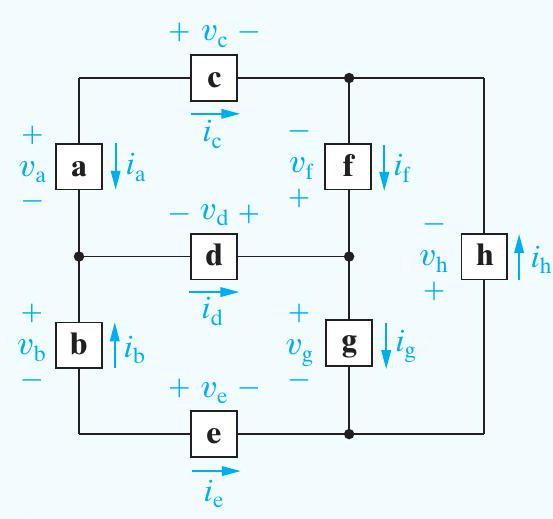
\includegraphics[max width=\textwidth]{2024_10_28_c0e2dc6a235cac59ec77g-042}
\end{center}

Figure 1.7 $\triangle$ Circuit model for power distribution in a home, with voltages and currents defined.

Note: Assess your understanding of the Practical Perspective by trying Chapter Problems 1.34 and 1.35.

\section*{Summary}
\begin{itemize}
  \item The International System of Units (SI) enables engineers to communicate in a meaningful way about quantitative results. Table 1.1 summarizes the base SI units; Table 1.2 presents some useful derived SI units. (See pages 8 and 9.)
  \item Circuit analysis is based on the variables of voltage and current. (See page 11.)
  \item Voltage is the energy per unit charge created by charge separation and has the SI unit of volt ( $v=d w / d q)$. (See page 12.)
  \item Current is the rate of charge flow and has the SI unit of ampere $(i=d q / d t)$. (See page 12. )
  \item The ideal basic circuit element is a two-terminal component that cannot be subdivided; it can be described mathematically in terms of its terminal voltage and current. (See page 12.)
  \item The passive sign convention uses a positive sign in the expression that relates the voltage and current at the terminals of an element when the reference direction for the current through the element is in the direction of the reference voltage drop across the element. (See page 13.)
  \item Power is energy per unit of time and is equal to the product of the terminal voltage and current; it has the SI unit of watt $(p=d w / d t=v i)$. (See page 15.)
  \item The algebraic sign of power is interpreted as follows:
  \item If $p>0$, power is being delivered to the circuit or circuit component.
  \item If $p<0$, power is being extracted from the circuit or circuit component. (See page 16.)
\end{itemize}

\section*{Problems}
\section*{Section 1.2}
1.1 There are approximately 260 million passenger vehicles registered in the United States. Assume that the battery in the average vehicle stores 540 watt-hours ( Wh ) of energy. Estimate (in gigawatt-hours) the total energy stored in U.S. passenger vehicles.\\
1.2 A hand-held video player displays $480 \times 320$ picture elements (pixels) in each frame of the video. Each pixel requires 2 bytes of memory. Videos are displayed at a rate of 30 frames per second. How many hours of video will fit in a 32 gigabyte memory?\\
1.3 The 16 giga-byte ( $\mathrm{GB}=2^{30}$ bytes) flash memory chip for an MP3 player is 11 mm by 15 mm by 1 mm . This memory chip holds 20,000 photos.\\
a) How many photos fit into a cube whose sides are 1 mm ?\\
b) How many bytes of memory are stored in a cube whose sides are $200 \mu \mathrm{~m}$ ?\\
1.4 The line described in Assessment Problem 1.7 is 845 mi in length. The line contains four conductors, each weighing 2526 lb per 1000 ft . How many kilograms of conductor are in the line?\\
1.5 One liter ( L ) of paint covers approximately $10 \mathrm{~m}^{2}$ of wall. How thick is the layer before it dries? (Hint: $1 \mathrm{~L}=1 \times 10^{6} \mathrm{~mm}^{3}$.)\\
1.6 Some species of bamboo can grow $250 \mathrm{~mm} /$ day. Assume individual cells in the plant are $10 \mu \mathrm{~m}$ long.\\
a) How long, on average, does it take a bamboo stalk to grow 1 cell length?\\
b) How many cell lengths are added in one week, on average?

\section*{Section 1.4}
1.7 There is no charge at the upper terminal of the element in Fig. 1.5 for $t<0$. At $t=0$ a current of $125 \mathrm{e}^{-2500 t} \mathrm{~mA}$ enters the upper terminal.\\
a) Derive the expression for the charge that accumulates at the upper terminal for $t>0$.\\
b) Find the total charge that accumulates at the upper terminal.\\
c) If the current is stopped at $t=0.5 \mathrm{~ms}$, how much charge has accumulated at the upper terminal?\\
1.8 The current entering the upper terminal of Fig. 1.5 is

$$
i=20 \cos 5000 t \mathrm{~A}
$$

Assume the charge at the upper terminal is zero at the instant the current is passing through its maximum value. Find the expression for $q(t)$.\\
1.9 The current at the terminals of the element in Fig. 1.5 is

$$
\begin{array}{ll}
i=0, & t<0 \\
i=40 t e^{-500 t} \mathrm{~A}, & t \geq 0
\end{array}
$$

a) Find the expression for the charge accumulating at the upper terminal.\\
b) Find the charge that has accumulated at $t=1 \mathrm{~ms}$.\\
1.10 In electronic circuits it is not unusual to encounter currents in the microampere range. Assume a $35 \mu \mathrm{~A}$ current, due to the flow of electrons. What is the average number of electrons per second that flow past a fixed reference cross section that is perpendicular to the direction of flow?\\
1.11 How much energy is imparted to an electron as it flows through a 6 V battery from the positive to the negative terminal? Express your answer in attojoules.

\section*{Sections 1.5-1.6}
1.12 The references for the voltage and current at the terminal of a circuit element are as shown in Fig.1.6(d). The numerical values for $v$ and $i$ are 40 V and -10 A .\\
a) Calculate the power at the terminals and state whether the power is being absorbed or delivered by the element in the box.\\
b) Given that the current is due to electron flow, state whether the electrons are entering or leaving terminal 2.\\
c) Do the electrons gain or lose energy as they pass through the element in the box?\\
1.13 Repeat Problem 1.12 with a voltage of -60 V .\\
1.14 Two electric circuits, represented by boxes A and B, are connected as shown in Fig. P1.14. The reference direction for the current $i$ in the interconnection and the reference polarity for the voltage $v$ across the interconnection are as shown in the figure. For each of the following sets of numerical values, calculate the power in the interconnection and state whether the power is flowing from A to B or vice versa.\\
a) $i=6 \mathrm{~A}, \quad v=30 \mathrm{~V}$\\
b) $i=-8 \mathrm{~A}, \quad v=-20 \mathrm{~V}$\\
c) $i=4 \mathrm{~A}, \quad v=-60 \mathrm{~V}$\\
d) $i=-9 \mathrm{~A}, \quad v=40 \mathrm{~V}$

Figure P1.14\\
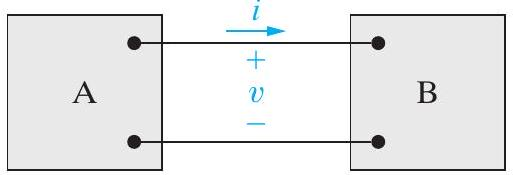
\includegraphics[max width=\textwidth, center]{2024_10_28_c0e2dc6a235cac59ec77g-044(1)}\\
1.15 When a car has a dead battery, it can often be started by connecting the battery from another car across its terminals. The positive terminals are connected together as are the negative terminals. The connection is illustrated in Fig. P1.15. Assume the current $i$ in Fig. P1.15 is measured and found to be 30 A .\\
a) Which car has the dead battery?\\
b) If this connection is maintained for 1 min , how much energy is transferred to the dead battery?

Figure P1.15\\
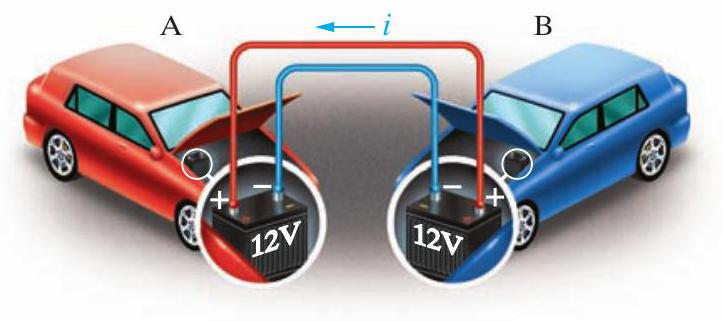
\includegraphics[max width=\textwidth, center]{2024_10_28_c0e2dc6a235cac59ec77g-044}\\
1.16 The manufacturer of a 1.5 V D flashlight battery says that the battery will deliver 9 mA for 40 continuous hours. During that time the voltage will drop from 1.5 V to 1.0 V . Assume the drop in voltage is linear with time. How much energy does the battery deliver in this 40 h interval?\\
1.17 One 12 V battery supplies 100 mA to a boom box. How much energy does the battery supply in 4 h ?\\
1.18 The voltage and current at the terminals of the circuit element in Fig. 1.5 are zero for $t<0$. For $t \geq 0$ they are

$$
\begin{aligned}
v & =15 \mathrm{e}^{-250 t} \mathrm{~V} \\
i & =40 e^{-250 t} \mathrm{~mA}
\end{aligned}
$$

a) Calculate the power supplied to the element at 10 ms .\\
b) Calculate the total energy delivered to the circuit element.\\
1.19 The voltage and current at the terminals of the cirPSpice cuit element in Fig. 1.5 are zero for $t<0$. For $t \geq 0$ Multisim they are

$$
\begin{aligned}
v & =75-75 e^{-1000 t} \mathrm{~V} \\
i & =50 e^{-1000 t} \mathrm{~mA}
\end{aligned}
$$

a) Find the maximum value of the power delivered to the circuit.\\
b) Find the total energy delivered to the element.\\
1.20 The voltage and current at the terminals of the circuit element in Fig. 1.5 are zero for $t<0$. For $t \geq 0$ they are

$$
\begin{aligned}
v & =50 e^{-1600 t}-50 e^{-400 t} \mathrm{~V} \\
i & =5 e^{-1600 t}-5 e^{-400 t} \mathrm{~mA}
\end{aligned}
$$

a) Find the power at $t=625 \mu \mathrm{~s}$.\\
b) How much energy is delivered to the circuit element between 0 and $625 \mu \mathrm{~s}$ ?\\
c) Find the total energy delivered to the element.\\
1.21 The voltage and current at the terminals of the cir$\underset{\text { PSprise }}{1.5}$ cuit element in Fig. 1.5 are zero for $t<0$. For $t \geq 0$ multisim they are

$$
\begin{aligned}
v & =(1500 t+1) e^{-750 t} \mathrm{~V}, & & t \geq 0 \\
i & =40 e^{-750 t} \mathrm{~mA}, & & t \geq 0
\end{aligned}
$$

a) Find the time when the power delivered to the circuit element is maximum.\\
b) Find the maximum value of $p$ in milliwatts.\\
c) Find the total energy delivered to the circuit element in microjoules.\\
1.22 The voltage and current at the terminals of the cirPSPice cuit element in Fig. 1.5 are zero for $t<0$. For $t \geq 0$ Multisim they are

$$
\begin{aligned}
v & =(3200 t+4) e^{-1000 t} \mathrm{~V} \\
i & =(128 t+0.16) e^{-1000 t} \mathrm{~A}
\end{aligned}
$$

a) At what instant of time is maximum power delivered to the element?\\
b) Find the maximum power in watts.\\
c) Find the total energy delivered to the element in microjoules.\\
1.23 The voltage and current at the terminals of the ${ }_{\text {PSprice }}$ circuit element in Fig. 1.5 are zero for $t<0$ and multsim $\quad t>40 \mathrm{~s}$. In the interval between 0 and 40 s the expressions are

$$
\begin{aligned}
v & =t(1-0.025 t) \mathrm{V}, \quad 0<t<40 \mathrm{~s} \\
i & =4-0.2 t \mathrm{~A}, \quad 0<t<40 \mathrm{~s}
\end{aligned}
$$

a) At what instant of time is the power being delivered to the circuit element maximum?\\
b) What is the power at the time found in part (a)?\\
c) At what instant of time is the power being extracted from the circuit element maximum?\\
d) What is the power at the time found in part (c)?\\
e) Calculate the net energy delivered to the circuit at $0,10,20,30$ and 40 s .\\
1.24 The voltage and current at the terminals of the cirPSPicE cuit element in Fig. 1.5 are zero for $t<0$. For $t \geq 0$ Mulisim they are

$$
\begin{aligned}
v & =400 e^{-100 t} \sin 200 t \mathrm{~V} \\
i & =5 e^{-100 t} \sin 200 t \mathrm{~A}
\end{aligned}
$$

a) Find the power absorbed by the element at $t=10 \mathrm{~ms}$.\\
b) Find the total energy absorbed by the element.\\
1.25 The voltage and current at the terminals of the elePSpice ment in Fig. 1.5 are\\
$v=250 \cos 800 \pi t \mathrm{~V}, \quad i=8 \sin 800 \pi t \mathrm{~A}$.\\
a) Find the maximum value of the power being delivered to the element.\\
b) Find the maximum value of the power being extracted from the element.\\
c) Find the average value of $p$ in the interval $0 \leq t \leq 2.5 \mathrm{~ms}$.\\
d) Find the average value of $p$ in the interval $0 \leq t \leq 15.625 \mathrm{~ms}$.\\
1.26 The voltage and current at the terminals of an autoPSpice mobile battery during a charge cycle are shown in Fig. P1.26.\\
a) Calculate the total charge transferred to the battery.\\
b) Calculate the total energy transferred to the battery.\\
c) Find the total energy delivered to the element.

Figure P1.26\\
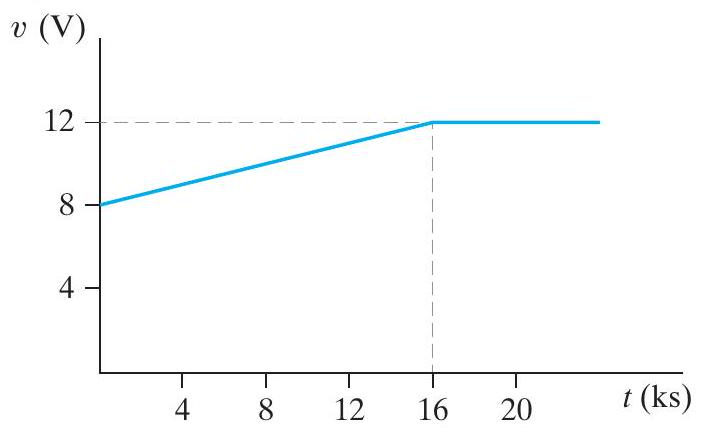
\includegraphics[max width=\textwidth, center]{2024_10_28_c0e2dc6a235cac59ec77g-045(3)}\\
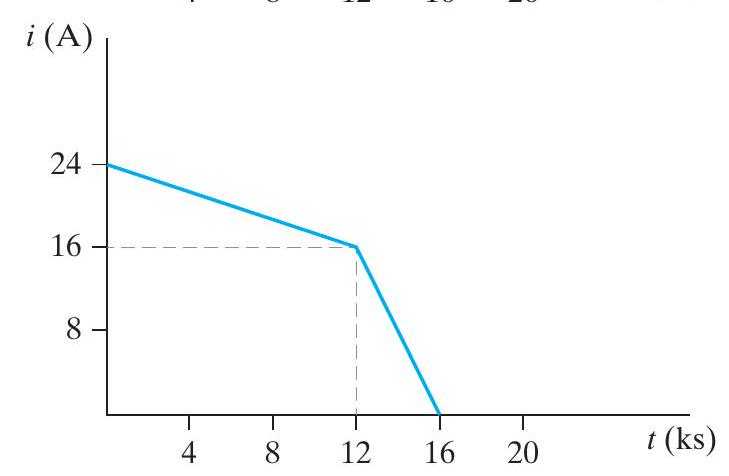
\includegraphics[max width=\textwidth, center]{2024_10_28_c0e2dc6a235cac59ec77g-045(2)}\\
1.27 The voltage and current at the terminals of the circuit element in Fig. 1.5 are shown in Fig. P1.27.\\
a) Sketch the power versus $t$ plot for $0 \leq t \leq 80 \mathrm{~ms}$.\\
b) Calculate the energy delivered to the circuit element at $t=10,30$, and 80 ms .

Figure P1.27\\
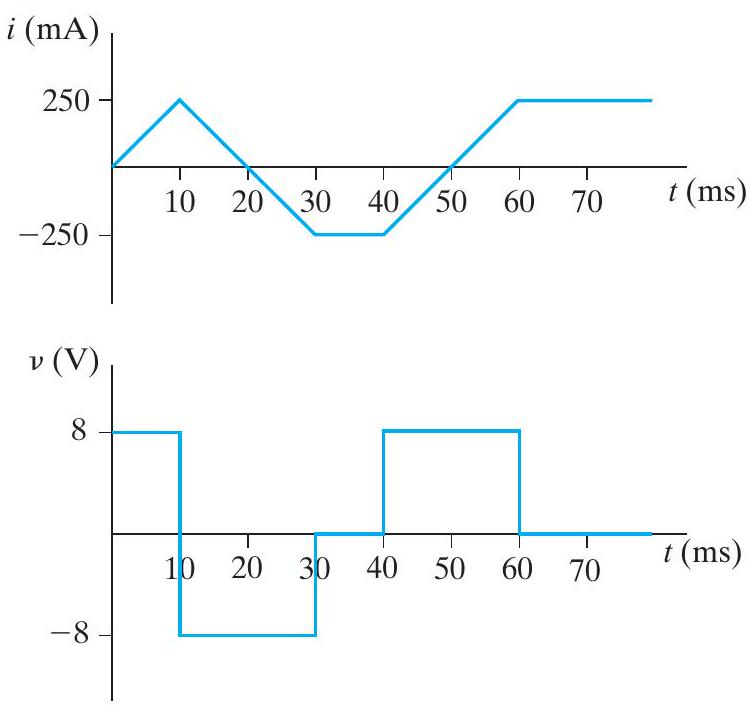
\includegraphics[max width=\textwidth, center]{2024_10_28_c0e2dc6a235cac59ec77g-045}\\
1.28 An industrial battery is charged over a period of several hours at a constant voltage of 120 V . Initially, the current is 10 mA and increases linearly to 15 mA in 10 ks . From 10 ks to 20 ks , the current is constant at 15 mA . From 20 ks to 30 ks the current decreases linearly to 10 mA . At 30 ks the power is disconnected from the battery.\\
a) Sketch the current from $t=0$ to $t=30 \mathrm{ks}$.\\
b) Sketch the power delivered to the battery from $t=0$ to $t=30 \mathrm{ks}$.\\
c) Using the sketch of the power, find the total energy delivered to the battery.\\
1.29 The numerical values for the currents and voltages in the circuit in Fig. P1.29 are given in Table P1.29. Find the total power developed in the circuit.

Figure P1.29\\
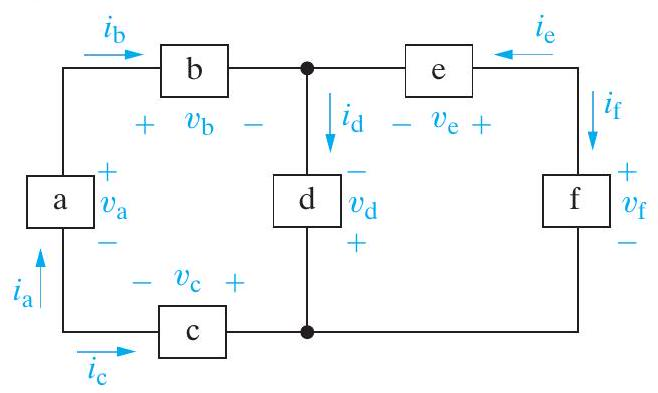
\includegraphics[max width=\textwidth, center]{2024_10_28_c0e2dc6a235cac59ec77g-045(1)}

\section*{TABLE P1.29}
\begin{center}
\begin{tabular}{lcc}
Element & Voltage (V) & Current (mA) \\
\hline
a & 40 & -4 \\
b & -24 & -4 \\
c & -16 & 4 \\
d & -80 & -1.5 \\
e & 40 & 2.5 \\
f & 120 & -2.5 \\
\hline
\end{tabular}
\end{center}

1.30 The numerical values of the voltages and currents in the interconnection seen in Fig. P1.30 are given in Table P1.30. Does the interconnection satisfy the power check?

Figure P1.30\\
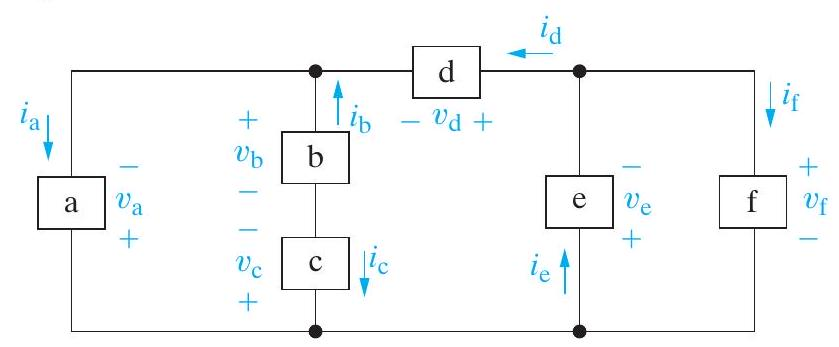
\includegraphics[max width=\textwidth, center]{2024_10_28_c0e2dc6a235cac59ec77g-046}

TABLE P1.30\\
Element\\
Voltage (kV)\\
Current $(\mu \mathrm{A})$

\begin{center}
\begin{tabular}{lrr}
a & -3 & -250 \\
b & 4 & -400 \\
c & 1 & 400 \\
d & 1 & 150 \\
e & -4 & 200 \\
f & 4 & 50 \\
\hline
\end{tabular}
\end{center}

1.31 Assume you are an engineer in charge of a project and one of your subordinate engineers reports that the interconnection in Fig. P1.31 does not pass the power check. The data for the interconnection are given in Table P1.31.\\
a) Is the subordinate correct? Explain your answer.\\
b) If the subordinate is correct, can you find the error in the data?

Figure P1.31\\
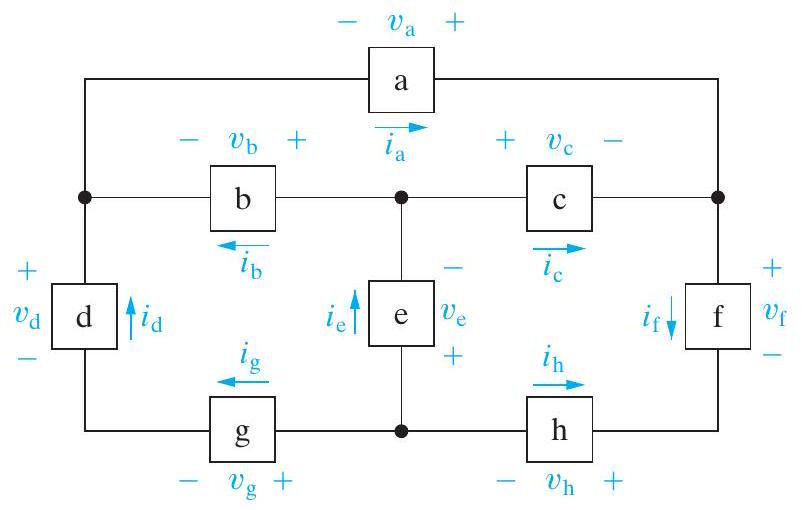
\includegraphics[max width=\textwidth, center]{2024_10_28_c0e2dc6a235cac59ec77g-046(1)}

\begin{center}
\begin{tabular}{lcc}
TABLE P1.31 &  &  \\
Element & Voltage (V) & Current (A) \\
\hline
a & 46.16 & 6.0 \\
b & 14.16 & 4.72 \\
c & -32.0 & -6.4 \\
d & 22.0 & 1.28 \\
e & -33.6 & -1.68 \\
f & 66.0 & 0.4 \\
g & 2.56 & 1.28 \\
h & -0.4 & 0.4 \\
\hline
\end{tabular}
\end{center}

1.32 The voltage and power values for each of the elements shown in Fig. P1.32 are given in Table P1.32.\\
a) Show that the interconnection of the elements satisfies the power check.\\
b) Find the value of the current through each of the elements using the values of power and voltage and the current directions shown in the figure.

Figure P1.32\\
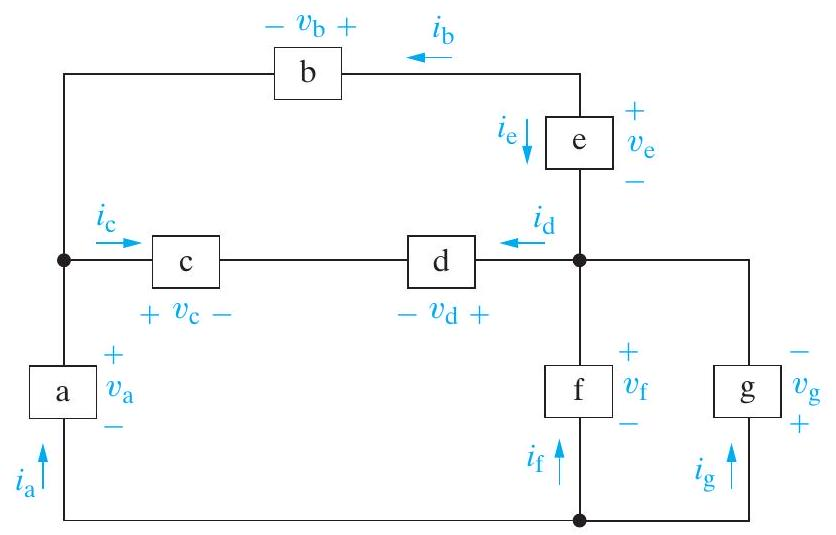
\includegraphics[max width=\textwidth, center]{2024_10_28_c0e2dc6a235cac59ec77g-046(2)}

\begin{center}
\begin{tabular}{llc}
TABLE P1.32 &  &  \\
Element & Power (kW) & Voltage (V) \\
\hline
a & 0.6 supplied & 400 \\
b & 0.05 supplied & -100 \\
c & 0.4 absorbed & 200 \\
d & 0.6 supplied & 300 \\
e & 0.1 absorbed & -200 \\
f & 2.0 absorbed & 500 \\
g & 1.25 supplied & -500 \\
\hline
\end{tabular}
\end{center}

1.33 The current and power for each of the interconnected elements in Fig. P1.33 is measured. The values are listed in Table P1.33.\\
a) Show that the interconnection satisfies the power check.\\
b) Identify the elements that absorb power.\\
c) Find the voltage for each of the elements in the interconnection, using the values of power and current and the voltage polarities shown in the figure.

Figure P1.33\\
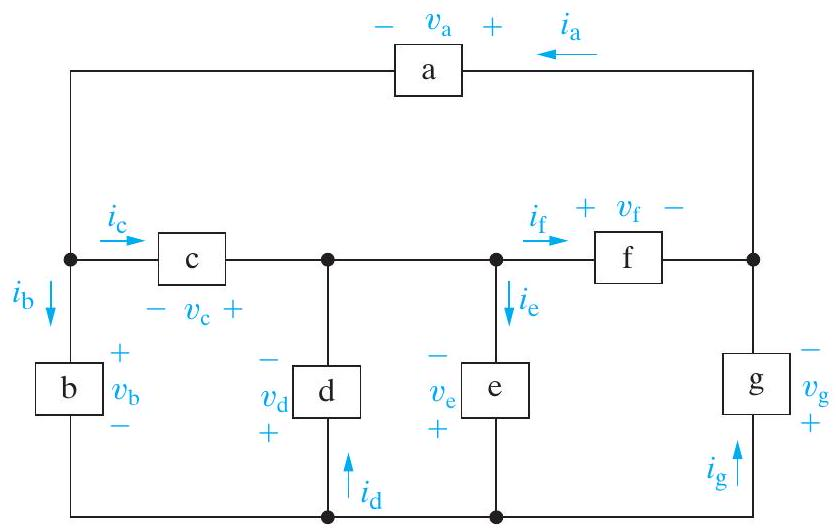
\includegraphics[max width=\textwidth, center]{2024_10_28_c0e2dc6a235cac59ec77g-047}

TABLE P1.33

\begin{center}
\begin{tabular}{lcc}
Element & Power (mW) & Current (mA) \\
\hline
a & 175 & 25 \\
b & 375 & 75 \\
c & 150 & -50 \\
d & -320 & 40 \\
e & 160 & 20 \\
f & 120 & -30 \\
g & -660 & 55 \\
\hline
\end{tabular}
\end{center}

1.34 Show that the power balances for the circuit shown in Fig. 1.7, using the voltage and current values given in Table 1.4, with the value of the current for component d changed to -1 A .\\
1.35 Suppose there is no power lost in the wires used to distribute power in a typical home.\\
a) Create a new model for the power distribution circuit by modifying the circuit shown in Fig 1.7. Use the same names, voltage polarities, and current directions for the components that remain in this modified model.\\
b) The following voltages and currents are calculated for the components:

$$
\begin{array}{ll}
v_{\mathrm{a}}=120 \mathrm{~V} & i_{\mathrm{a}}=-10 \mathrm{~A} \\
v_{\mathrm{b}}=120 \mathrm{~V} & i_{\mathrm{b}}=10 \mathrm{~A} \\
v_{\mathrm{f}}=-120 \mathrm{~V} & i_{\mathrm{f}}=3 \mathrm{~A} \\
v_{\mathrm{g}}=120 \mathrm{~V} & \\
v_{\mathrm{h}}=-240 \mathrm{~V} & i_{\mathrm{h}}=-7 \mathrm{~A}
\end{array}
$$

If the power in this modified model balances, what is the value of the current in component g ?

\section*{CHAPTER}
\begin{center}

\includegraphics[max width=\textwidth]{2024_10_28_c0e2dc6a235cac59ec77g-048}
\end{center}

\section*{CHAPTER CONTENTS}
2.1 Voltage and Current Sources p. 26\\
2.2 Electrical Resistance (Ohm's Law) p. 30\\
2.3 Construction of a Circuit Model p. 34\\
2.4 Kirchhoff's Laws p. 37\\
2.5 Analysis of a Circuit Containing Dependent Sources p. 42

\section*{CHAPTER OBJECTIVES}
1 Understand the symbols for and the behavior of the following ideal basic circuit elements: independent voltage and current sources, dependent voltage and current sources, and resistors.\\
2 Be able to state Ohm's law, Kirchhoff's current law, and Kirchhoff's voltage law, and be able to use these laws to analyze simple circuits.\\
3 Know how to calculate the power for each element in a simple circuit and be able to determine whether or not the power balances for the whole circuit.

\section*{Circuit Elements}
There are five ideal basic circuit elements: voltage sources, current sources, resistors, inductors, and capacitors. In this chapter we discuss the characteristics of voltage sources, current sources, and resistors. Although this may seem like a small number of elements with which to begin analyzing circuits, many practical systems can be modeled with just sources and resistors. They are also a useful starting point because of their relative simplicity; the mathematical relationships between voltage and current in sources and resistors are algebraic. Thus you will be able to begin learning the basic techniques of circuit analysis with only algebraic manipulations.

We will postpone introducing inductors and capacitors until Chapter 6, because their use requires that you solve integral and differential equations. However, the basic analytical techniques for solving circuits with inductors and capacitors are the same as those introduced in this chapter. So, by the time you need to begin manipulating more difficult equations, you should be very familiar with the methods of writing them.

\section*{Practical Perspective}
\section*{Heating with Electric Radiators}
You want to heat your small garage using a couple of electric radiators. The power and voltage requirements for each radiator are $1200 \mathrm{~W}, 240 \mathrm{~V}$. But you are not sure how to wire the radiators to the power supplied to the garage. Should you use the wiring diagram on the left, or the one on the right? Does it make any difference?

Once you have studied the material in this chapter, you will be able to answer these questions and determine how to heat the garage. The Practical Perspective at the end of this chapter guides you through the analysis of two circuits based on the two wiring diagrams shown below.\\
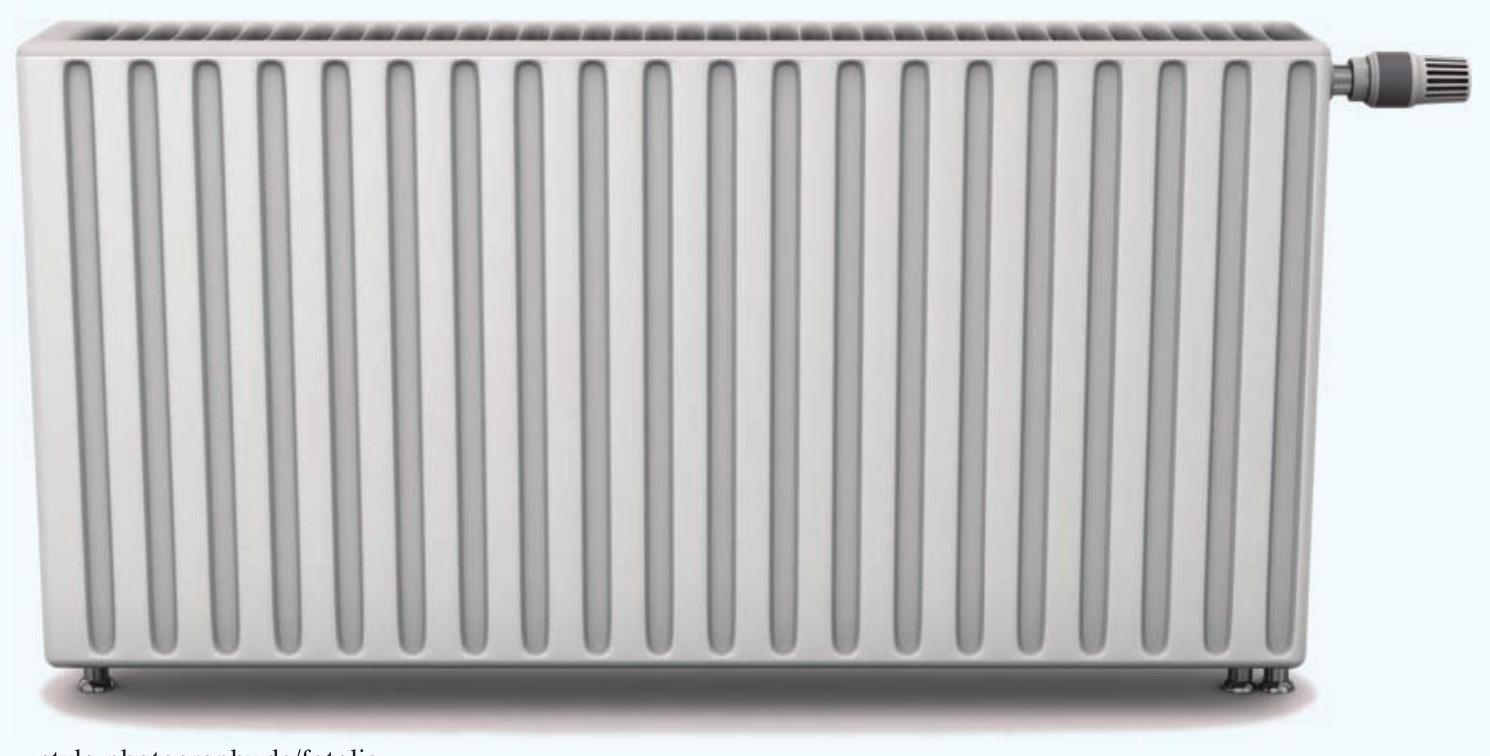
\includegraphics[max width=\textwidth, center]{2024_10_28_c0e2dc6a235cac59ec77g-049(1)}\\
\href{http://style-photography.de/fotolia}{style-photography.de/fotolia}\\
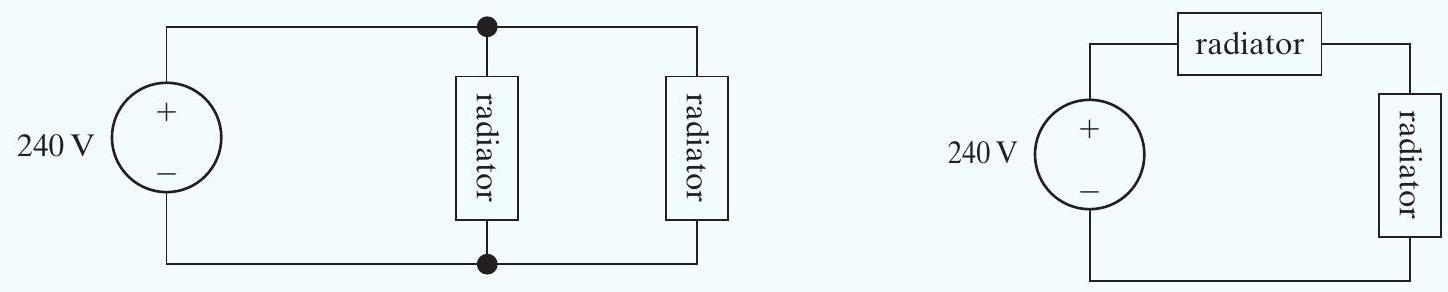
\includegraphics[max width=\textwidth, center]{2024_10_28_c0e2dc6a235cac59ec77g-049}\\
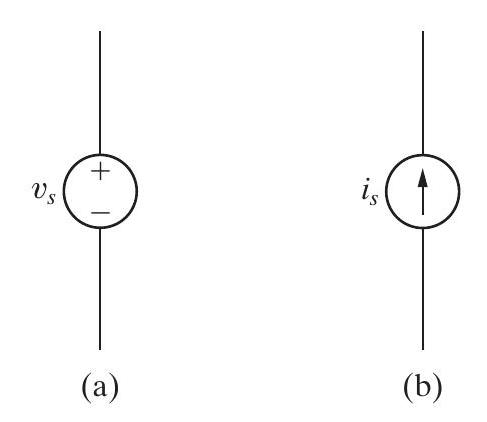
\includegraphics[max width=\textwidth, center]{2024_10_28_c0e2dc6a235cac59ec77g-050}

Figure 2.1 - The circuit symbols for (a) an ideal independent voltage source and (b) an ideal independent current source.

\subsection*{2.1 Voltage and Current Sources}
Before discussing ideal voltage and current sources, we need to consider the general nature of electrical sources. An electrical source is a device that is capable of converting nonelectric energy to electric energy and vice versa. A discharging battery converts chemical energy to electric energy, whereas a battery being charged converts electric energy to chemical energy. A dynamo is a machine that converts mechanical energy to electric energy and vice versa. If operating in the mechanical-to-electric mode, it is called a generator. If transforming from electric to mechanical energy, it is referred to as a motor. The important thing to remember about these sources is that they can either deliver or absorb electric power, generally maintaining either voltage or current. This behavior is of particular interest for circuit analysis and led to the creation of the ideal voltage source and the ideal current source as basic circuit elements. The challenge is to model practical sources in terms of the ideal basic circuit elements.

An ideal voltage source is a circuit element that maintains a prescribed voltage across its terminals regardless of the current flowing in those terminals. Similarly, an ideal current source is a circuit element that maintains a prescribed current through its terminals regardless of the voltage across those terminals. These circuit elements do not exist as practical devices-they are idealized models of actual voltage and current sources.

Using an ideal model for current and voltage sources places an important restriction on how we may describe them mathematically. Because an ideal voltage source provides a steady voltage, even if the current in the element changes, it is impossible to specify the current in an ideal voltage source as a function of its voltage. Likewise, if the only information you have about an ideal current source is the value of current supplied, it is impossible to determine the voltage across that current source. We have sacrificed our ability to relate voltage and current in a practical source for the simplicity of using ideal sources in circuit analysis.

Ideal voltage and current sources can be further described as either independent sources or dependent sources. An independent source establishes a voltage or current in a circuit without relying on voltages or currents elsewhere in the circuit. The value of the voltage or current supplied is specified by the value of the independent source alone. In contrast, a dependent source establishes a voltage or current whose value depends on the value of a voltage or current elsewhere in the circuit. You cannot specify the value of a dependent source unless you know the value of the voltage or current on which it depends.

The circuit symbols for the ideal independent sources are shown in Fig. 2.1. Note that a circle is used to represent an independent source. To completely specify an ideal independent voltage source in a circuit, you must include the value of the supplied voltage and the reference polarity, as shown in Fig. 2.1(a). Similarly, to completely specify an ideal independent current source, you must include the value of the supplied current and its reference direction, as shown in Fig. 2.1(b).

The circuit symbols for the ideal dependent sources are shown in Fig. 2.2. A diamond is used to represent a dependent source. Both the\\
dependent current source and the dependent voltage source may be controlled by either a voltage or a current elsewhere in the circuit, so there are a total of four variations, as indicated by the symbols in Fig. 2.2. Dependent sources are sometimes called controlled sources.

To completely specify an ideal dependent voltage-controlled voltage source, you must identify the controlling voltage, the equation that permits you to compute the supplied voltage from the controlling voltage, and the reference polarity for the supplied voltage. In Fig. 2.2(a), the controlling voltage is named $v_{x}$, the equation that determines the supplied voltage $v_{s}$ is

$$
v_{s}=\mu v_{x}
$$

and the reference polarity for $v_{s}$ is as indicated. Note that $\mu$ is a multiplying constant that is dimensionless.

Similar requirements exist for completely specifying the other ideal dependent sources. In Fig. 2.2(b), the controlling current is $i_{x}$, the equation for the supplied voltage $v_{s}$ is

$$
v_{s}=\rho i_{x}
$$

the reference polarity is as shown, and the multiplying constant $\rho$ has the dimension volts per ampere. In Fig. 2.2(c), the controlling voltage is $v_{x}$, the equation for the supplied current $i_{s}$ is

$$
i_{s}=\alpha v_{x}
$$

the reference direction is as shown, and the multiplying constant $\alpha$ has the dimension amperes per volt. In Fig. 2.2(d), the controlling current is $i_{x}$, the equation for the supplied current $i_{s}$ is

$$
i_{s}=\beta i_{x},
$$

the reference direction is as shown, and the multiplying constant $\beta$ is dimensionless.

Finally, in our discussion of ideal sources, we note that they are examples of active circuit elements. An active element is one that models a device capable of generating electric energy. Passive elements model physical devices that cannot generate electric energy. Resistors, inductors, and capacitors are examples of passive circuit elements. Examples 2.1 and 2.2 illustrate how the characteristics of ideal independent and dependent sources limit the types of permissible interconnections of the sources.\\
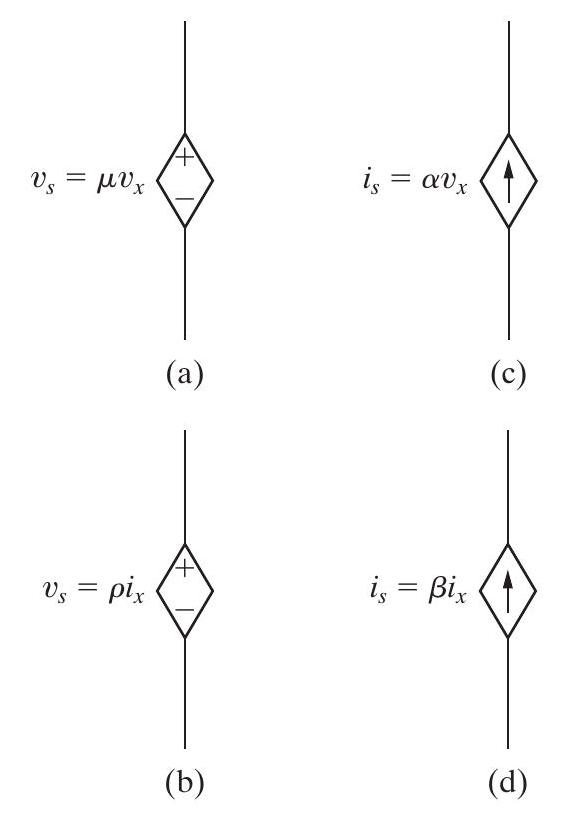
\includegraphics[max width=\textwidth, center]{2024_10_28_c0e2dc6a235cac59ec77g-051}

Figure 2.2 The circuit symbols for (a) an ideal dependent voltage-controlled voltage source, (b) an ideal dependent current-controlled voltage source, (c) an ideal dependent voltage-controlled current source, and (d) an ideal dependent current-controlled current source.

\section*{Example 2.1 $\quad$ Testing Interconnections of Ideal Sources}
Using the definitions of the ideal independent voltage and current sources, state which interconnections in Fig. 2.3 are permissible and which violate the constraints imposed by the ideal sources.

\section*{Solution}
Connection (a) is valid. Each source supplies voltage across the same pair of terminals, marked a,b. This requires that each source supply the same voltage with the same polarity, which they do.

Connection (b) is valid. Each source supplies current through the same pair of terminals, marked a,b. This requires that each source supply the same current in the same direction, which they do.

Connection (c) is not permissible. Each source supplies voltage across the same pair of terminals, marked a,b. This requires that each source supply the same voltage with the same polarity, which they do not.

Connection (d) is not permissible. Each source supplies current through the same pair of terminals, marked a,b. This requires that each source supply the same current in the same direction, which they do not.

Connection (e) is valid. The voltage source supplies voltage across the pair of terminals marked a,b. The current source supplies current through the same pair of terminals. Because an ideal voltage source supplies the same voltage regardless of the current, and an ideal current source supplies the same current regardless of the voltage, this is a permissible connection.\\
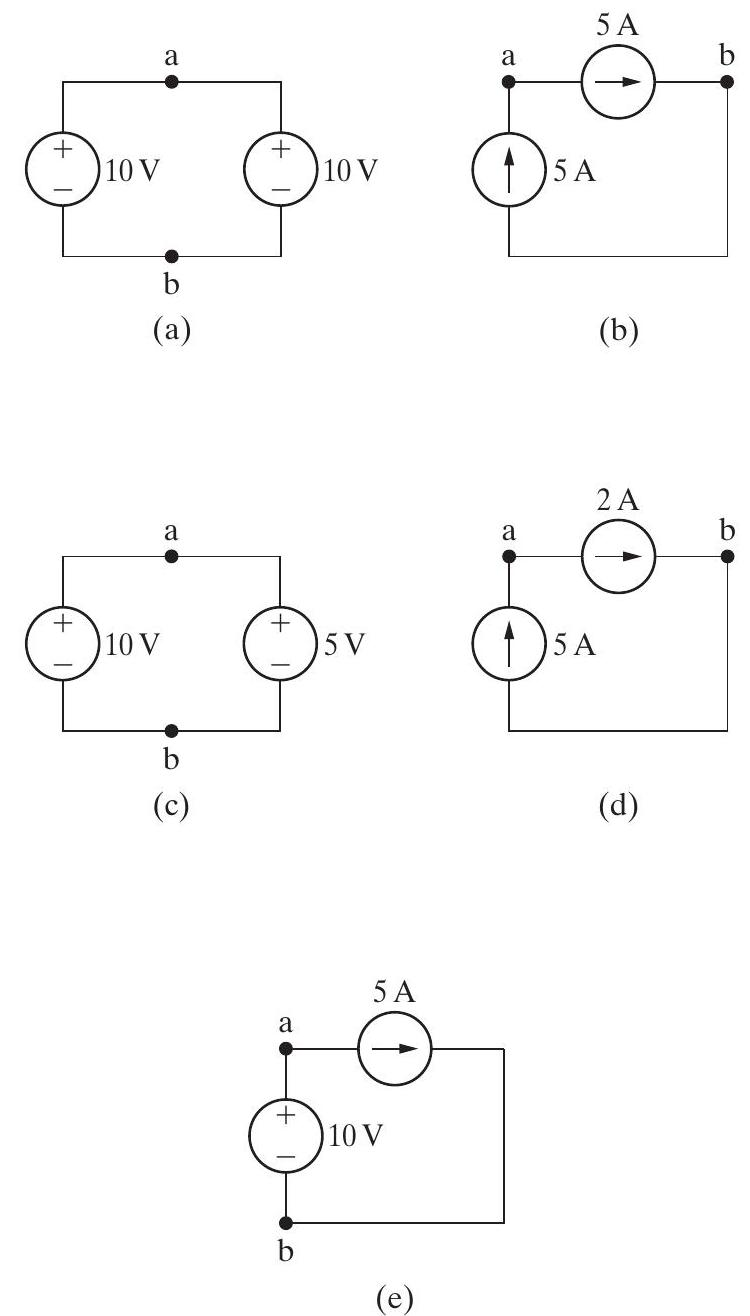
\includegraphics[max width=\textwidth, center]{2024_10_28_c0e2dc6a235cac59ec77g-052}

Figure 2.3 $\boldsymbol{\Delta}$ The circuits for Example 2.1.

\section*{Example 2.2 Testing Interconnections of Ideal Independent and Dependent Sources}
Using the definitions of the ideal independent and dependent sources, state which interconnections in Fig. 2.4 are valid and which violate the constraints imposed by the ideal sources.

\section*{Solution}
Connection (a) is invalid. Both the independent source and the dependent source supply voltage across the same pair of terminals, labeled a,b. This requires that each source supply the same voltage with the same polarity. The independent source supplies 5 V , but the dependent source supplies 15 V .

Connection (b) is valid. The independent voltage source supplies voltage across the pair of terminals marked a,b. The dependent current source supplies current through the same pair of terminals. Because an ideal voltage source supplies the same voltage regardless of current, and an ideal current source supplies the same current regardless of voltage, this is an allowable connection.

Connection (c) is valid. The independent current source supplies current through the pair of terminals marked a,b. The dependent voltage source supplies voltage across the same pair of terminals. Because an ideal current source supplies the same current regardless of voltage, and an ideal voltage source supplies the same voltage regardless of current, this is an allowable connection.

Connection (d) is invalid. Both the independent source and the dependent source supply current through the same pair of terminals, labeled a,b. This requires that each source supply the same current in the same reference direction. The independent source supplies 2 A , but the dependent source supplies 6 A in the opposite direction.\\
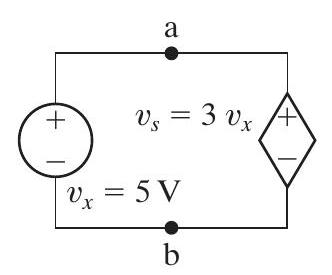
\includegraphics[max width=\textwidth, center]{2024_10_28_c0e2dc6a235cac59ec77g-053(3)}\\
(a)\\
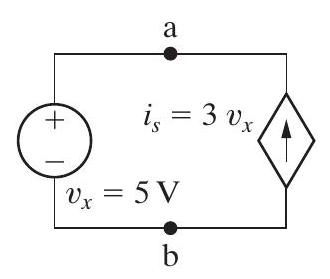
\includegraphics[max width=\textwidth, center]{2024_10_28_c0e2dc6a235cac59ec77g-053(1)}\\
(b)\\
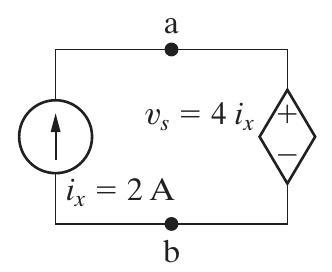
\includegraphics[max width=\textwidth, center]{2024_10_28_c0e2dc6a235cac59ec77g-053}\\
(c)\\
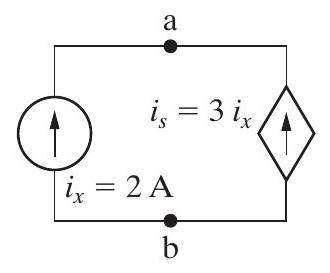
\includegraphics[max width=\textwidth, center]{2024_10_28_c0e2dc6a235cac59ec77g-053(2)}\\
(d)

Figure 2.4 $\Delta$ The circuits for Example 2.2.

\section*{ASSESSMENT PROBLEMS}
\section*{Objective 1—Understand ideal basic circuit elements}
2.1 For the circuit shown,\\
a) What value of $v_{g}$ is required in order for the interconnection to be valid?\\
b) For this value of $v_{g}$, find the power associated with the 8 A source.

Answer: (a) -2 V ;\\
(b) -16 W (16 W delivered).\\
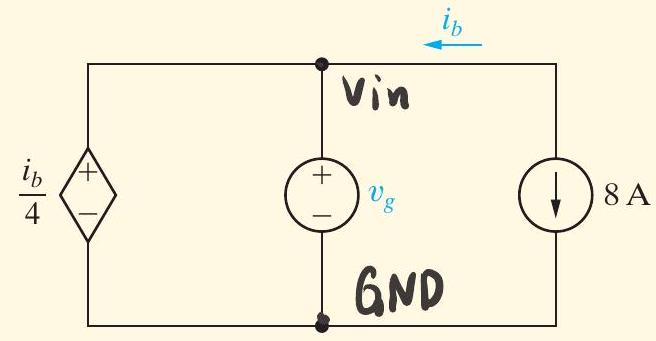
\includegraphics[max width=\textwidth, center]{2024_10_28_c0e2dc6a235cac59ec77g-054(3)}

NOTE: Also try Chapter Problems 2.6 and 2.7.\\
2.2 For the circuit shown,\\
a) What value of $\alpha$ is required in order for the interconnection to be valid?\\
b) For the value of $\alpha$ calculated in part (a), find the power associated with the 25 V source.

Answer: (a) $0.6 \mathrm{~A} / \mathrm{V}$;\\
(b) 375 W (375 W absorbed).\\
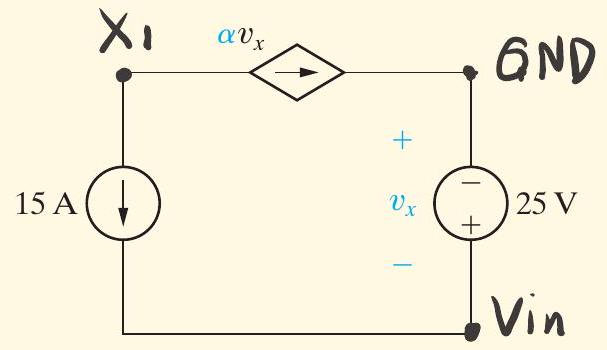
\includegraphics[max width=\textwidth, center]{2024_10_28_c0e2dc6a235cac59ec77g-054(1)}\\
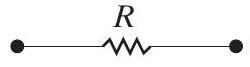
\includegraphics[max width=\textwidth, center]{2024_10_28_c0e2dc6a235cac59ec77g-054}

Figure 2.5 $\Delta$ The circuit symbol for a resistor having a resistance $R$.\\
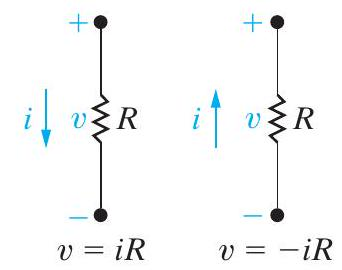
\includegraphics[max width=\textwidth, center]{2024_10_28_c0e2dc6a235cac59ec77g-054(2)}

Figure 2.6 $\triangle$ Two possible reference choices for the current and voltage at the terminals of a resistor, and the resulting equations.

\subsection*{2.2 Electrical Resistance (Ohm's Law)}
Resistance is the capacity of materials to impede the flow of current or, more specifically, the flow of electric charge. The circuit element used to model this behavior is the resistor. Figure 2.5 shows the circuit symbol for the resistor, with $R$ denoting the resistance value of the resistor.

Conceptually, we can understand resistance if we think about the moving electrons that make up electric current interacting with and being resisted by the atomic structure of the material through which they are moving. In the course of these interactions, some amount of electric energy is converted to thermal energy and dissipated in the form of heat. This effect may be undesirable. However, many useful electrical devices take advantage of resistance heating, including stoves, toasters, irons, and space heaters.

Most materials exhibit measurable resistance to current. The amount of resistance depends on the material. Metals such as copper and aluminum have small values of resistance, making them good choices for wiring used to conduct electric current. In fact, when represented in a circuit diagram, copper or aluminum wiring isn't usually modeled as a resistor; the resistance of the wire is so small compared to the resistance of other elements in the circuit that we can neglect the wiring resistance to simplify the diagram.

For purposes of circuit analysis, we must reference the current in the resistor to the terminal voltage. We can do so in two ways: either in the direction of the voltage drop across the resistor or in the direction of the voltage rise across the resistor, as shown in Fig. 2.6. If we choose the former, the relationship between the voltage and current is


\begin{equation*}
v=i R \tag{2.1}
\end{equation*}


where

$$
\begin{aligned}
v & =\text { the voltage in volts, } \\
i & =\text { the current in amperes, } \\
R & =\text { the resistance in ohms. }
\end{aligned}
$$

If we choose the second method, we must write


\begin{equation*}
v=-i R \tag{2.2}
\end{equation*}


where $v, i$, and $R$ are, as before, measured in volts, amperes, and ohms, respectively. The algebraic signs used in Eqs. 2.1 and 2.2 are a direct consequence of the passive sign convention, which we introduced in Chapter 1.

Equations 2.1 and 2.2 are known as Ohm's law after Georg Simon Ohm, a German physicist who established its validity early in the nineteenth century. Ohm's law is the algebraic relationship between voltage and current for a resistor. In SI units, resistance is measured in ohms. The Greek letter omega $(\Omega)$ is the standard symbol for an ohm. The circuit diagram symbol for an $8 \Omega$ resistor is shown in Fig. 2.7.

Ohm's law expresses the voltage as a function of the current. However, expressing the current as a function of the voltage also is convenient. Thus, from Eq. 2.1,


\begin{equation*}
i=\frac{v}{R} \tag{2.3}
\end{equation*}


or, from Eq. 2.2,


\begin{equation*}
i=-\frac{v}{R} \tag{2.4}
\end{equation*}


The reciprocal of the resistance is referred to as conductance, is symbolized by the letter $G$, and is measured in siemens (S). Thus,


\begin{equation*}
G=\frac{1}{R} \mathrm{~S} \tag{2.5}
\end{equation*}


An $8 \Omega$ resistor has a conductance value of 0.125 S . In much of the professional literature, the unit used for conductance is the mho (ohm spelled backward), which is symbolized by an inverted omega ( $($ ). Therefore we may also describe an $8 \Omega$ resistor as having a conductance of 0.125 mho, ( $\mho$ ).

We use ideal resistors in circuit analysis to model the behavior of physical devices. Using the qualifier ideal reminds us that the resistor model makes several simplifying assumptions about the behavior of actual resistive devices. The most important of these simplifying assumptions is that the resistance of the ideal resistor is constant and its value does not vary over time. Most actual resistive devices do not have constant resistance, and their resistance does vary over time. The ideal resistor model can be used to represent a physical device whose resistance doesn't vary much from some constant value over the time period of interest in the circuit analysis. In this book we assume that the simplifying assumptions about resistance devices are valid, and we thus use ideal resistors in circuit analysis.

We may calculate the power at the terminals of a resistor in several ways. The first approach is to use the defining equation and simply calculate

Figure 2.7 $\triangle$ The circuit symbol for an $8 \Omega$ resistor.\\
the product of the terminal voltage and current. For the reference systems shown in Fig. 2.6, we write


\begin{equation*}
p=v i \tag{2.6}
\end{equation*}


when $v=i R$ and


\begin{equation*}
p=-v i \tag{2.7}
\end{equation*}


when $v=-i R$.\\
A second method of expressing the power at the terminals of a resistor expresses power in terms of the current and the resistance. Substituting Eq. 2.1 into Eq. 2.6, we obtain

$$
p=v i=(i R) i
$$

so

Power in a resistor in terms of current $\cdot$

Power in a resistor in terms of voltage


\begin{equation*}
p=i^{2} R \tag{2.8}
\end{equation*}


Likewise, substituting Eq. 2.2 into Eq. 2.7, we have


\begin{equation*}
p=-v i=-(-i R) i=i^{2} R \tag{2.9}
\end{equation*}


Equations 2.8 and 2.9 are identical and demonstrate clearly that, regardless of voltage polarity and current direction, the power at the terminals of a resistor is positive. Therefore, a resistor absorbs power from the circuit.

A third method of expressing the power at the terminals of a resistor is in terms of the voltage and resistance. The expression is independent of the polarity references, so


\begin{equation*}
p=\frac{v^{2}}{R} \tag{2.10}
\end{equation*}


Sometimes a resistor's value will be expressed as a conductance rather than as a resistance. Using the relationship between resistance and conductance given in Eq. 2.5, we may also write Eqs. 2.9 and 2.10 in terms of the conductance, or


\begin{align*}
p & =\frac{i^{2}}{G}  \tag{2.11}\\
p & =v^{2} G \tag{2.12}
\end{align*}


Equations 2.6-2.12 provide a variety of methods for calculating the power absorbed by a resistor. Each yields the same answer. In analyzing a circuit, look at the information provided and choose the power equation that uses that information directly.

Example 2.3 illustrates the application of Ohm's law in conjunction with an ideal source and a resistor. Power calculations at the terminals of a resistor also are illustrated.

\section*{Example 2.3 Calculating Voltage, Current, and Power for a Simple Resistive Circuit}
In each circuit in Fig. 2.8, either the value of $v$ or $i$ is not known.\\
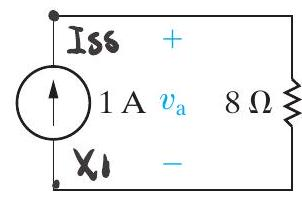
\includegraphics[max width=\textwidth, center]{2024_10_28_c0e2dc6a235cac59ec77g-057(1)}\\
(a)\\
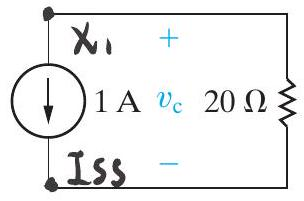
\includegraphics[max width=\textwidth, center]{2024_10_28_c0e2dc6a235cac59ec77g-057(4)}\\
(c)\\
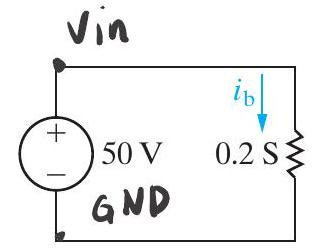
\includegraphics[max width=\textwidth, center]{2024_10_28_c0e2dc6a235cac59ec77g-057(2)}\\
(b)\\
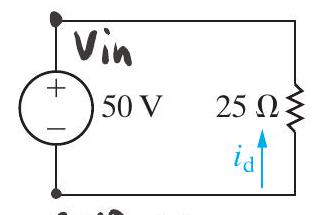
\includegraphics[max width=\textwidth, center]{2024_10_28_c0e2dc6a235cac59ec77g-057(3)}\\
(d)

Figure $2.8 \boldsymbol{\Delta}$ The circuits for Example 2.3.\\
a) Calculate the values of $v$ and $i$.\\
b) Determine the power dissipated in each resistor.

\section*{Solution}
a) The voltage $v_{a}$ in Fig. 2.8(a) is a drop in the direction of the current in the resistor. Therefore,

$$
v_{\mathrm{a}}=(1)(8)=8 \mathrm{~V} \text {. }
$$

The current $i_{b}$ in the resistor with a conductance of 0.2 S in Fig. 2.8(b) is in the direction of the voltage drop across the resistor. Thus

$$
i_{\mathrm{b}}=(50)(0.2)=10 \mathrm{~A}
$$

The voltage $v_{c}$ in Fig. 2.8(c) is a rise in the direction of the current in the resistor. Hence

$$
v_{\mathrm{c}}=-(1)(20)=-20 \mathrm{~V}
$$

The current $i_{\mathrm{d}}$ in the $25 \Omega$ resistor in Fig. 2.8(d) is in the direction of the voltage rise across the resistor. Therefore

$$
i_{\mathrm{d}}=\frac{-50}{25}=-2 \mathrm{~A}
$$

b) The power dissipated in each of the four resistors is

$$
\begin{aligned}
p_{8 \Omega} & =\frac{(8)^{2}}{8}=(1)^{2}(8)=8 \mathrm{~W} \\
p_{0.2 S} & =(50)^{2}(0.2)=500 \mathrm{~W} \\
p_{20 \Omega} & =\frac{(-20)^{2}}{20}=(1)^{2}(20)=20 \mathrm{~W} \\
p_{25 \Omega} & =\frac{(50)^{2}}{25}=(-2)^{2}(25)=100 \mathrm{~W}
\end{aligned}
$$

\section*{ASSESSMENT PROBLEMS}
\section*{Objective 2-Be able to state and use Ohm's Law . . .}
2.3 For the circuit shown,\\
a) If $v_{g}=1 \mathrm{kV}$ and $i_{g}=5 \mathrm{~mA}$, find the value of $R$ and the power absorbed by the resistor.\\
b) If $i_{g}=75 \mathrm{~mA}$ and the power delivered by the voltage source is 3 W , find $v_{g}, R$, and the power absorbed by the resistor.\\
c) If $R=300 \Omega$ and the power absorbed by $R$ is 480 mW , find $i_{g}$ and $v_{g}$.\\
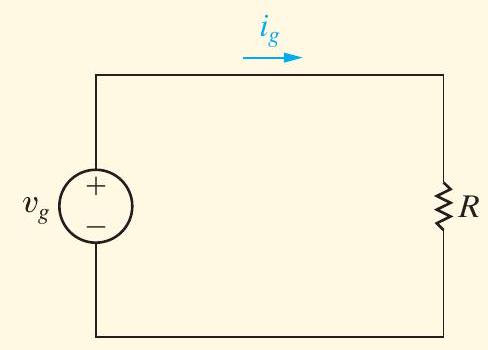
\includegraphics[max width=\textwidth, center]{2024_10_28_c0e2dc6a235cac59ec77g-057}

Answer: (a) $200 \mathrm{k} \Omega, 5 \mathrm{~W}$;\\
(b) $40 \mathrm{~V}, 533.33 \Omega, 3 \mathrm{~W}$;\\
(c) $40 \mathrm{~mA}, 12 \mathrm{~V}$.

NOTE: Also try Chapter Problems 2.11 and 2.12.\\
2.4 For the circuit shown,\\
a) If $i_{g}=0.5 \mathrm{~A}$ and $G=50 \mathrm{mS}$, find $v_{g}$ and the power delivered by the current source.\\
b) If $v_{g}=15 \mathrm{~V}$ and the power delivered to the conductor is 9 W , find the conductance $G$ and the source current $i_{g}$.\\
c) If $G=200 \mu \mathrm{~S}$ and the power delivered to the conductance is 8 W , find $i_{g}$ and $v_{g}$.\\
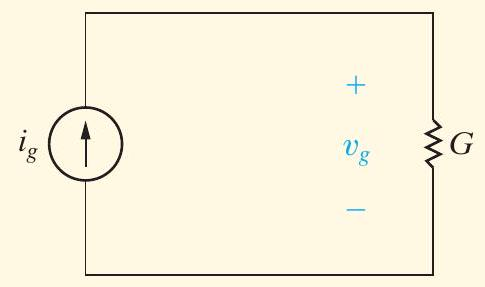
\includegraphics[max width=\textwidth, center]{2024_10_28_c0e2dc6a235cac59ec77g-057(5)}

Answer: (a) $10 \mathrm{~V}, 5 \mathrm{~W}$;\\
(b) $40 \mathrm{mS}, 0.6 \mathrm{~A}$;\\
(c) $40 \mathrm{~mA}, 200 \mathrm{~V}$.

Having introduced the general characteristics of ideal sources and resistors, we next show how to use these elements to build the circuit model of a practical system.

\subsection*{2.3 Construction of a Circuit Model}
We have already stated that one reason for an interest in the basic circuit elements is that they can be used to construct circuit models of practical systems. The skill required to develop a circuit model of a device or system is as complex as the skill required to solve the derived circuit. Although this text emphasizes the skills required to solve circuits, you also will need other skills in the practice of electrical engineering, and one of the most important is modeling.

We develop circuit models in the next two examples. In Example 2.4 we construct a circuit model based on a knowledge of the behavior of the system's components and how the components are interconnected. In Example 2.5 we create a circuit model by measuring the terminal behavior of a device.

\section*{Example 2.4 Constructing a Circuit Model of a Flashlight}
Construct a circuit model of a flashlight.

\section*{Solution}
We chose the flashlight to illustrate a practical system because its components are so familiar. Figure 2.9 shows a photograph of a widely available flashlight.

When a flashlight is regarded as an electrical system, the components of primary interest are the batteries, the lamp, the connector, the case, and the switch. We now consider the circuit model for each component.

A dry-cell battery maintains a reasonably constant terminal voltage if the current demand is not excessive. Thus if the dry-cell battery is operating within its intended limits, we can model it with an ideal voltage source. The prescribed voltage then is constant and equal to the sum of two dry-cell values.

The ultimate output of the lamp is light energy, which is achieved by heating the filament in the lamp to a temperature high enough to cause radiation in the visible range. We can model the lamp with an ideal resistor. Note in this case that although the resistor accounts for the amount of electric energy converted to thermal energy, it does not predict how much of the thermal energy is converted to light energy. The resistor used to represent the lamp does predict the steady current drain on the batteries, a characteristic of the system that also is of interest. In this model, $R_{l}$ symbolizes the lamp resistance.

The connector used in the flashlight serves a dual role. First, it provides an electrical conductive path between the dry cells and the case. Second, it is\\
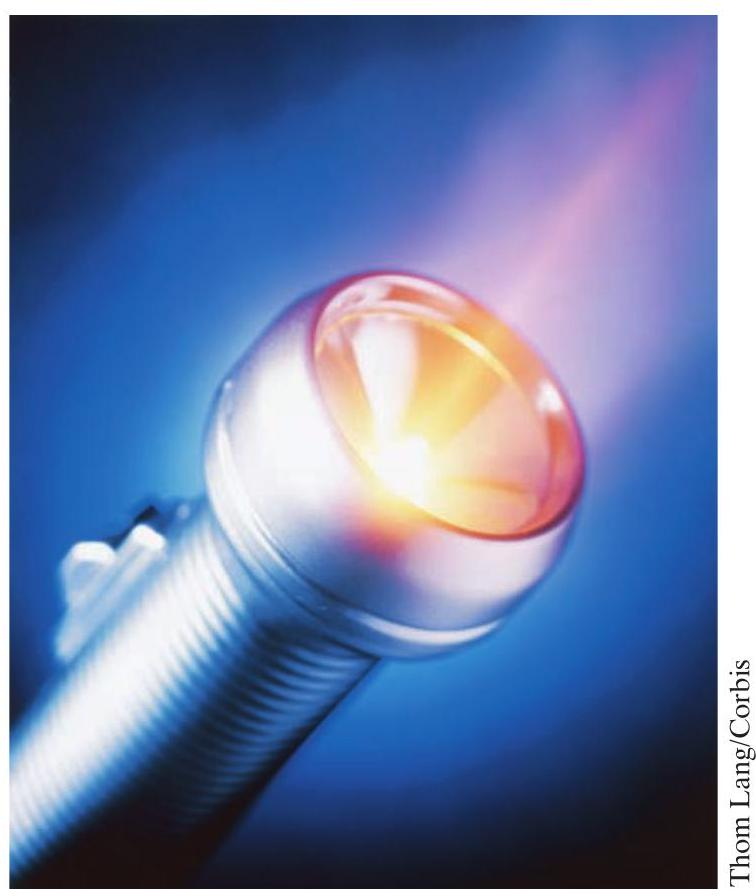
\includegraphics[max width=\textwidth, center]{2024_10_28_c0e2dc6a235cac59ec77g-058}

Figure 2.9 A A flashlight can be viewed as an electrical system.\\
formed into a springy coil so that it also can apply mechanical pressure to the contact between the batteries and the lamp. The purpose of this mechanical pressure is to maintain contact between the two dry cells and between the dry cells and the lamp. Hence, in choosing the wire for the connector, we may find that its mechanical properties are more\\
important than its electrical properties for the flashlight design. Electrically, we can model the connector with an ideal resistor, labeled $R_{1}$.

The case also serves both a mechanical and an electrical purpose. Mechanically, it contains all the other components and provides a grip for the person using it. Electrically, it provides a connection between other elements in the flashlight. If the case is metal, it conducts current between the batteries and the lamp. If it is plastic, a metal strip inside the case connects the coiled connector to the switch. Either way, an ideal resistor, which we denote $R_{c}$, models the electrical connection provided by the case.

The final component is the switch. Electrically, the switch is a two-state device. It is either on or OFF. An ideal switch offers no resistance to the current when it is in the on state, but it offers infinite resistance to current when it is in the OFF state. These two states represent the limiting values of a resistor; that is, the on state corresponds to a resistor with a numerical value of zero, and the off state corresponds to a resistor with a numerical value of infinity. The two extreme values have the descriptive names short circuit $(R=0)$ and open circuit ( $R=\infty$ ). Figure 2.10(a) and (b) show the graphical representation of a short circuit and an open circuit, respectively. The symbol shown in Fig. 2.10(c) represents the fact that a switch can be either a short circuit or an open circuit, depending on the position of its contacts.

We now construct the circuit model of the flashlight. Starting with the dry-cell batteries, the positive terminal of the first cell is connected to the negative terminal of the second cell, as shown in Fig. 2.11. The positive terminal of the second cell is connected to one terminal of the lamp. The other terminal of the lamp makes contact with one side of the switch, and the other side of the switch is connected to the metal case. The metal case is then connected to the negative terminal of the first dry cell by means of the metal spring. Note that the elements form a closed path or circuit. You can see the closed path formed by the connected elements in Fig. 2.11. Figure 2.12 shows a circuit model for the flashlight.\\
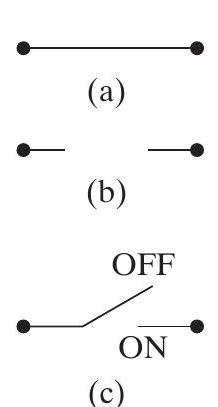
\includegraphics[max width=\textwidth, center]{2024_10_28_c0e2dc6a235cac59ec77g-059(1)}

Figure $2.10 \boldsymbol{\Delta}$ Circuit symbols. (a) Short circuit. (b) Open circuit. (c) Switch.\\
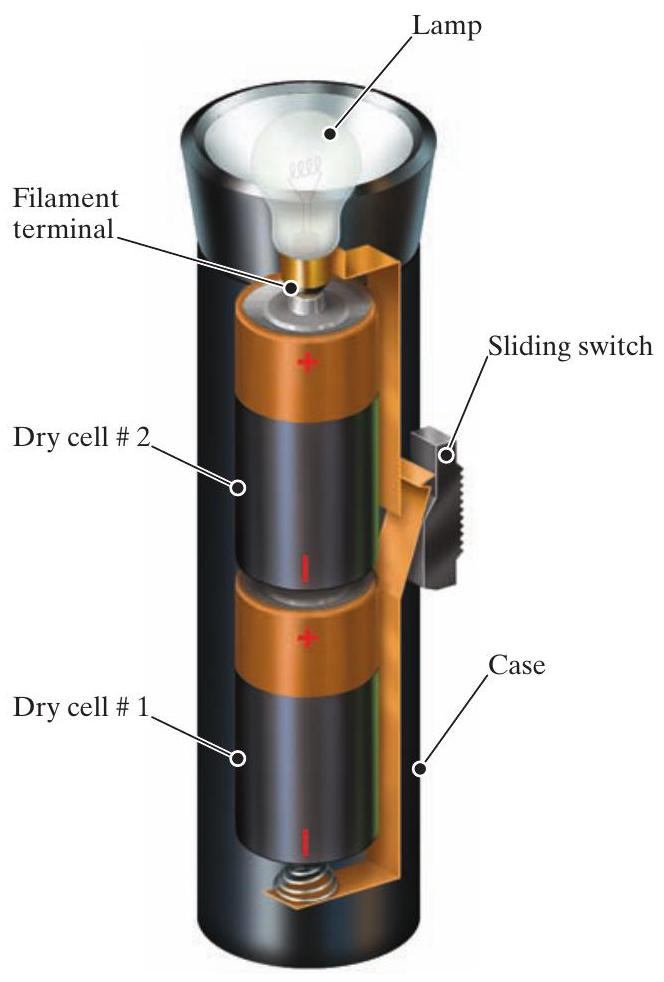
\includegraphics[max width=\textwidth, center]{2024_10_28_c0e2dc6a235cac59ec77g-059(2)}

Figure $2.11 \boldsymbol{\Delta}$ The arrangement of flashlight components.\\
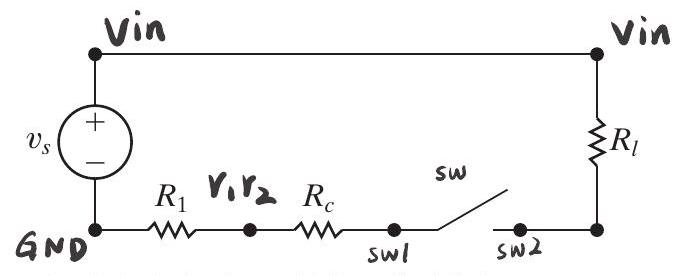
\includegraphics[max width=\textwidth, center]{2024_10_28_c0e2dc6a235cac59ec77g-059}

Figure $2.12 \triangle$ A circuit model for a flashlight.

We can make some general observations about modeling from our flashlight example: First, in developing a circuit model, the electrical behavior of each physical component is of primary interest. In the flashlight model, three very different physical components - a lamp, a coiled wire, and a metal case-are all represented by the same circuit element (a resistor), because the electrical phenomenon taking place in each is the same. Each is presenting resistance to the current flowing through the circuit.

Second, circuit models may need to account for undesired as well as desired electrical effects. For example, the heat resulting from the resistance in the lamp produces the light, a desired effect. However, the heat\\
resulting from the resistance in the case and coil represents an unwanted or parasitic effect. It drains the dry cells and produces no useful output. Such parasitic effects must be considered or the resulting model may not adequately represent the system.

And finally, modeling requires approximation. Even for the basic system represented by the flashlight, we made simplifying assumptions in developing the circuit model. For example, we assumed an ideal switch, but in practical switches, contact resistance may be high enough to interfere with proper operation of the system. Our model does not predict this behavior. We also assumed that the coiled connector exerts enough pressure to eliminate any contact resistance between the dry cells. Our model does not predict the effect of inadequate pressure. Our use of an ideal voltage source ignores any internal dissipation of energy in the dry cells, which might be due to the parasitic heating just mentioned. We could account for this by adding an ideal resistor between the source and the lamp resistor. Our model assumes the internal loss to be negligible.

In modeling the flashlight as a circuit, we had a basic understanding of and access to the internal components of the system. However, sometimes we know only the terminal behavior of a device and must use this information in constructing the model. Example 2.5 explores such a modeling problem.

\section*{Example 2.5 Constructing a Circuit Model Based on Terminal Measurements}
The voltage and current are measured at the terminals of the device illustrated in Fig. 2.13(a), and the values of $v_{t}$ and $i_{t}$ are tabulated in Fig. 2.13(b). Construct a circuit model of the device inside the box.\\
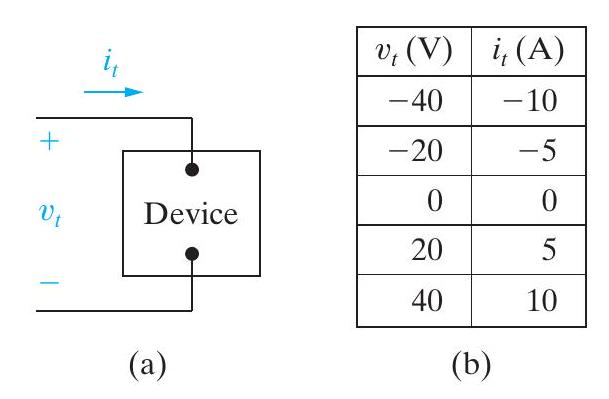
\includegraphics[max width=\textwidth, center]{2024_10_28_c0e2dc6a235cac59ec77g-060(1)}

\section*{Solution}
Plotting the voltage as a function of the current yields the graph shown in Fig. 2.14(a). The equation of the line in this figure illustrates that the terminal voltage is directly proportional to the terminal current, $v_{t}=4 i_{t}$. In terms of Ohm's law, the device inside the box behaves like a $4 \Omega$ resistor. Therefore, the circuit model for the device inside the box is a $4 \Omega$ resistor, as seen in Fig. 2.14(b).

We come back to this technique of using terminal characteristics to construct a circuit model after introducing Kirchhoff's laws and circuit analysis.

Figure 2.13 $\Delta$ The (a) device and (b) data for Example 2.5.\\
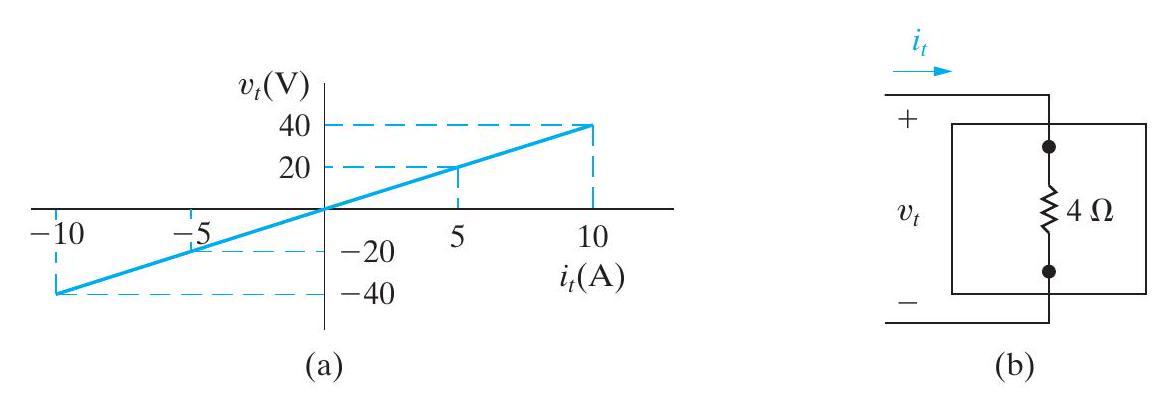
\includegraphics[max width=\textwidth, center]{2024_10_28_c0e2dc6a235cac59ec77g-060}

Figure $2.14 \boldsymbol{\Delta}$ (a) The values of $v_{t}$ versus $i_{t}$ for the device in Fig. 2.13. (b) The circuit model for the device in Fig. 2.13.

NOTE: Assess your understanding of this example by trying Chapter Problems 2.14 and 2.15.

\subsection*{2.4 Kirchhoff's Laws}
A circuit is said to be solved when the voltage across and the current in every element have been determined. Ohm's law is an important equation for deriving such solutions. However, Ohm's law may not be enough to provide a complete solution. As we shall see in trying to solve the flashlight circuit from Example 2.4, we need to use two more important algebraic relationships, known as Kirchhoff's laws, to solve most circuits.

We begin by redrawing the circuit as shown in Fig. 2.15, with the switch in the on state. Note that we have also labeled the current and voltage variables associated with each resistor and the current associated with the voltage source. Labeling includes reference polarities, as always. For convenience, we attach the same subscript to the voltage and current labels as we do to the resistor labels. In Fig. 2.15, we also removed some of the terminal dots of Fig. 2.12 and have inserted nodes. Terminal dots are the start and end points of an individual circuit element. A node is a point where two or more circuit elements meet. It is necessary to identify nodes in order to use Kirchhoff's current law, as we will see in a moment. In Fig. 2.15, the nodes are labeled a, b, c, and d. Node d connects the battery and the lamp and in essence stretches all the way across the top of the diagram, though we label a single point for convenience. The dots on either side of the switch indicate its terminals, but only one is needed to represent a node, so only one is labeled node c.

For the circuit shown in Fig. 2.15, we can identify seven unknowns: $i_{s}, i_{1}, i_{c}, i_{l}, v_{1}, v_{c}$, and $v_{l}$. Recall that $v_{s}$ is a known voltage, as it represents the sum of the terminal voltages of the two dry cells, a constant voltage of 3 V . The problem is to find the seven unknown variables. From algebra, you know that to find $n$ unknown quantities you must solve $n$ simultaneous independent equations. From our discussion of Ohm's law in Section 2.2, you know that three of the necessary equations are


\begin{gather*}
v_{1}=i_{1} R_{1}  \tag{2.13}\\
v_{c}=i_{c} R_{c}  \tag{2.14}\\
v_{l}=i_{l} R_{l} \tag{2.15}
\end{gather*}


What about the other four equations?\\
The interconnection of circuit elements imposes constraints on the relationship between the terminal voltages and currents. These constraints are referred to as Kirchhoff's laws, after Gustav Kirchhoff, who first stated them in a paper published in 1848. The two laws that state the constraints in mathematical form are known as Kirchhoff's current law and Kirchhoff's voltage law.

We can now state Kirchhoff's current law:

The algebraic sum of all the currents at any node in a circuit equals zero.

To use Kirchhoff's current law, an algebraic sign corresponding to a reference direction must be assigned to every current at the node. Assigning a positive sign to a current leaving a node requires assigning a negative sign to a current entering a node. Conversely, giving a negative sign to a current leaving a node requires giving a positive sign to a current entering a node.\\
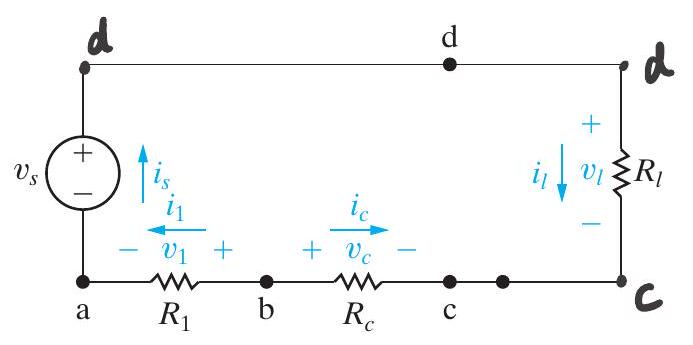
\includegraphics[max width=\textwidth, center]{2024_10_28_c0e2dc6a235cac59ec77g-061}

Figure $2.15 \boldsymbol{\Delta}$ Circuit model of the flashlight with assigned voltage and current variables.

Kirchhoff's current law (KCL)

\section*{Kirchhoff's voltage law (KVL)}
Applying Kirchhoff's current law to the four nodes in the circuit shown in Fig. 2.15, using the convention that currents leaving a node are considered positive, yields four equations:

\[
\begin{array}{cc}
\text { node } \mathrm{a} & i_{s}-i_{1}=0, \\
\text { node } \mathrm{b} & i_{1}+i_{c}=0, \\
\text { node } \mathrm{c} & -i_{c}-i_{l}=0 \\
\text { node } \mathrm{d} & i_{l}-i_{s}=0 \tag{2.19}
\end{array}
\]

Note that Eqs. 2.16-2.19 are not an independent set, because any one of the four can be derived from the other three. In any circuit with $n$ nodes, $n-1$ independent current equations can be derived from Kirchhoff's current law. ${ }^{1}$ Let's disregard Eq. 2.19 so that we have six independent equations, namely, Eqs. 2.13-2.18. We need one more, which we can derive from Kirchhoff's voltage law.

Before we can state Kirchhoff's voltage law, we must define a closed path or loop. Starting at an arbitrarily selected node, we trace a closed path in a circuit through selected basic circuit elements and return to the original node without passing through any intermediate node more than once. The circuit shown in Fig. 2.15 has only one closed path or loop. For example, choosing node a as the starting point and tracing the circuit clockwise, we form the closed path by moving through nodes $\mathrm{d}, \mathrm{c}, \mathrm{b}$, and back to node a. We can now state Kirchhoff's voltage law:

The algebraic sum of all the voltages around any closed path in a circuit equals zero.

To use Kirchhoff's voltage law, we must assign an algebraic sign (reference direction) to each voltage in the loop. As we trace a closed path, a voltage will appear either as a rise or a drop in the tracing direction. Assigning a positive sign to a voltage rise requires assigning a negative sign to a voltage drop. Conversely, giving a negative sign to a voltage rise requires giving a positive sign to a voltage drop.

We now apply Kirchhoff's voltage law to the circuit shown in Fig. 2.15. We elect to trace the closed path clockwise, assigning a positive algebraic sign to voltage drops. Starting at node d leads to the expression


\begin{equation*}
v_{l}-v_{c}+v_{1}-v_{s}=0 \tag{2.20}
\end{equation*}


which represents the seventh independent equation needed to find the seven unknown circuit variables mentioned earlier.

The thought of having to solve seven simultaneous equations to find the current delivered by a pair of dry cells to a flashlight lamp is not very appealing. Thus in the coming chapters we introduce you to analytical techniques that will enable you to solve a simple one-loop circuit by writing a single equation. However, before moving on to a discussion of these circuit techniques, we need to make several observations about the detailed analysis of the flashlight circuit. In general, these observations are true and therefore are important to the discussions in subsequent chapters. They also support the contention that the flashlight circuit can be solved by defining a single unknown.

\footnotetext{$\overline{1}$ We say more about this observation in Chapter 4.
}First, note that if you know the current in a resistor, you also know the voltage across the resistor, because current and voltage are directly related through Ohm's law. Thus you can associate one unknown variable with each resistor, either the current or the voltage. Choose, say, the current as the unknown variable. Then, once you solve for the unknown current in the resistor, you can find the voltage across the resistor. In general, if you know the current in a passive element, you can find the voltage across it, greatly reducing the number of simultaneous equations to be solved. For example, in the flashlight circuit, we eliminate the voltages $v_{c}$, $v_{l}$, and $v_{1}$ as unknowns. Thus at the outset we reduce the analytical task to solving four simultaneous equations rather than seven.

The second general observation relates to the consequences of connecting only two elements to form a node. According to Kirchhoff's current law, when only two elements connect to a node, if you know the current in one of the elements, you also know it in the second element. In other words, you need define only one unknown current for the two elements. When just two elements connect at a single node, the elements are said to be in series. The importance of this second observation is obvious when you note that each node in the circuit shown in Fig. 2.15 involves only two elements. Thus you need to define only one unknown current. The reason is that Eqs. 2.16-2.18 lead directly to


\begin{equation*}
i_{s}=i_{1}=-i_{c}=i_{l} \tag{2.21}
\end{equation*}


which states that if you know any one of the element currents, you know them all. For example, choosing to use $i_{s}$ as the unknown eliminates $i_{1}, i_{c}$, and $i_{l}$. The problem is reduced to determining one unknown, namely, $i_{s}$.

Examples 2.6 and 2.7 illustrate how to write circuit equations based on Kirchhoff's laws. Example 2.8 illustrates how to use Kirchhoff's laws and Ohm's law to find an unknown current. Example 2.9 expands on the technique presented in Example 2.5 for constructing a circuit model for a device whose terminal characteristics are known.

\section*{Example 2.6 Using Kirchhoff's Current Law}
Sum the currents at each node in the circuit shown in Fig. 2.16. Note that there is no connection $\operatorname{dot}(\bullet)$ in the center of the diagram, where the $4 \Omega$ branch crosses the branch containing the ideal current source $i_{\mathrm{a}}$.

\section*{Solution}
In writing the equations, we use a positive sign for a current leaving a node. The four equations are\\
node a $\quad i_{1}+i_{4}-i_{2}-i_{5}=0$,\\
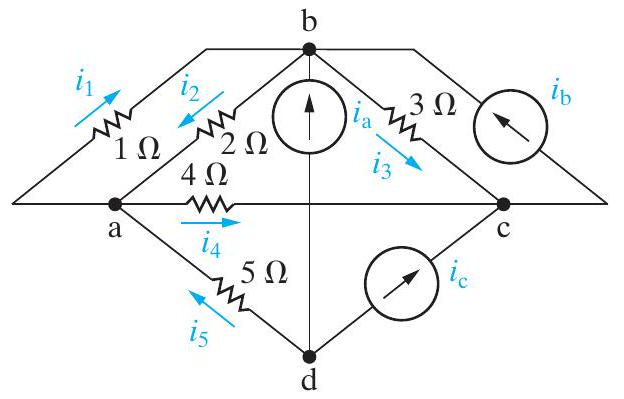
\includegraphics[max width=\textwidth, center]{2024_10_28_c0e2dc6a235cac59ec77g-063}

Figure $2.16 \boldsymbol{\Delta}$ The circuit for Example 2.6.\\
node $\mathrm{b} \quad i_{2}+i_{3}-i_{1}-i_{\mathrm{b}}-i_{\mathrm{a}}=0$,\\
node $\mathrm{c} \quad i_{\mathrm{b}}-i_{3}-i_{4}-i_{\mathrm{c}}=0$,\\
node d

$$
i_{5}+i_{\mathrm{a}}+\mathrm{i}_{\mathrm{c}}=0
$$

\section*{Example 2.7 Using Kirchhoff's Voltage Law}
Sum the voltages around each designated path in the circuit shown in Fig. 2.17.

\section*{Solution}
In writing the equations, we use a positive sign for a voltage drop. The four equations are

$$
\begin{array}{lr}
\text { path a } & -v_{1}+v_{2}+v_{4}-v_{\mathrm{b}}-v_{3}=0 \\
\text { path } \mathrm{b} & -v_{\mathrm{a}}+v_{3}+v_{5}=0 \\
\text { path c } & v_{\mathrm{b}}-v_{4}-v_{\mathrm{c}}-v_{6}-v_{5}=0 \\
\text { path d } & -v_{\mathrm{a}}-v_{1}+v_{2}-v_{\mathrm{c}}+v_{7}-v_{\mathrm{d}}=0
\end{array}
$$

\begin{center}
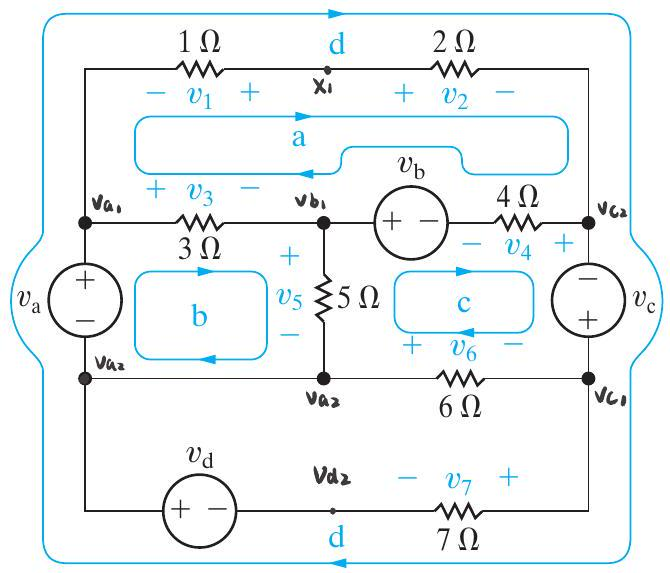
\includegraphics[max width=\textwidth]{2024_10_28_c0e2dc6a235cac59ec77g-064(2)}
\end{center}

Figure 2.17 The circuit for Example 2.7.

\section*{Example 2.8 Applying Ohm's Law and Kirchhoff's Laws to Find an Unknown Current}
a) Use Kirchhoff's laws and Ohm's law to find $i_{o}$ in the circuit shown in Fig. 2.18.\\
\includegraphics[max width=\textwidth, center]{2024_10_28_c0e2dc6a235cac59ec77g-064}

Figure $2.18 \triangle$ The circuit for Example 2.8.\\
b) Test the solution for $i_{o}$ by verifying that the total power generated equals the total power dissipated.

\section*{Solution}
a) We begin by redrawing the circuit and assigning an unknown current to the $50 \Omega$ resistor and unknown voltages across the $10 \Omega$ and $50 \Omega$ resistors. Figure 2.19 shows the circuit. The nodes are labeled $\mathrm{a}, \mathrm{b}$, and c to aid the discussion.\\
\includegraphics[max width=\textwidth, center]{2024_10_28_c0e2dc6a235cac59ec77g-064(1)}

Figure 2.19 $\Delta$ The circuit shown in Fig. 2.18, with the unknowns $i_{1}, v_{o}$, and $v_{1}$ defined.

Because $i_{o}$ also is the current in the 120 V source, we have two unknown currents and\\
therefore must derive two simultaneous equations involving $i_{o}$ and $i_{1}$. We obtain one of the equations by applying Kirchhoff's current law to either node b or c . Summing the currents at node b and assigning a positive sign to the currents leaving the node gives

$$
i_{1}-i_{o}-6=0
$$

We obtain the second equation from Kirchhoff's voltage law in combination with Ohm's law. Noting from Ohm's law that $v_{o}$ is $10 i_{o}$ and $v_{1}$ is $50 i_{1}$, we sum the voltages around the closed path cabc to obtain

$$
-120+10 i_{o}+50 i_{1}=0
$$

In writing this equation, we assigned a positive sign to voltage drops in the clockwise direction. Solving these two equations for $i_{o}$ and $i_{1}$ yields

$$
i_{o}=-3 \mathrm{~A} \quad \text { and } \quad i_{1}=3 \mathrm{~A} .
$$

b) The power dissipated in the $50 \Omega$ resistor is

$$
p_{50 \Omega}=(3)^{2}(50)=450 \mathrm{~W} .
$$

The power dissipated in the $10 \Omega$ resistor is

$$
p_{10 \Omega}=(-3)^{2}(10)=90 \mathrm{~W}
$$

The power delivered to the 120 V source is

$$
p_{120 \mathrm{~V}}=-120 i_{o}=-120(-3)=360 \mathrm{~W}
$$

The power delivered to the 6 A source is\\
$p_{6 \mathrm{~A}}=-v_{1}(6)$, but $\quad v_{1}=50 i_{1}=150 \mathrm{~V}$.

Therefore

$$
p_{6 \mathrm{~A}}=-150(6)=-900 \mathrm{~W}
$$

The 6 A source is delivering 900 W , and the 120 V source is absorbing 360 W . The total power absorbed is $360+450+90=900 \mathrm{~W}$. Therefore, the solution verifies that the power delivered equals the power absorbed.

\section*{Example 2.9 Constructing a Circuit Model Based on Terminal Measurements}
The terminal voltage and terminal current were measured on the device shown in Fig. 2.20(a), and the values of $v_{t}$ and $i_{t}$ are tabulated in Fig. 2.20(b).\\
\includegraphics[max width=\textwidth, center]{2024_10_28_c0e2dc6a235cac59ec77g-065}\\
(a)

\begin{center}
\begin{tabular}{|c|c|}
\hline
$v_{t}(\mathrm{~V})$ & $i_{t}(\mathrm{~A})$ \\
\hline
30 & 0 \\
\hline
15 & 3 \\
\hline
0 & 6 \\
\hline
\end{tabular}
\end{center}

(b)

Figure 2.20 A (a) Device and (b) data for Example 2.9.\\
a) Construct a circuit model of the device inside the box.\\
b) Using this circuit model, predict the power this device will deliver to a $10 \Omega$ resistor.

\section*{Solution}
a) Plotting the voltage as a function of the current yields the graph shown in Fig. 2.21(a). The equation of the line plotted is

$$
v_{t}=30-5 i_{t}
$$

Now we need to identify the components of a circuit model that will produce the same relationship between voltage and current. Kirchhoff's voltage law tells us that the voltage drops across two components in series. From the equation, one of those components produces a 30 V drop regardless of the current. This component can be modeled as an ideal independent voltage source. The other component produces a positive voltage drop in the direction of the current $i_{t}$. Because the voltage drop is proportional to the current, Ohm's law tells us that this component can be modeled as an ideal resistor with a value of $5 \Omega$. The resulting circuit model is depicted in the dashed box in Fig. 2.21(b).\\
\includegraphics[max width=\textwidth, center]{2024_10_28_c0e2dc6a235cac59ec77g-065(1)}

Figure $2.21 \triangle$ (a) The graph of $v_{t}$ versus $i_{t}$ for the device in Fig. 2.20(a). (b) The resulting circuit model for the device in Fig. 2.20(a), connected to a $10 \Omega$ resistor.\\
b) Now we attach a $10 \Omega$ resistor to the device in Fig. 2.21(b) to complete the circuit. Kirchhoff's current law tells us that the current in the $10 \Omega$ resistor is the same as the current in the $5 \Omega$ resistor. Using Kirchhoff's voltage law and Ohm's law, we can write the equation for the voltage drops around the circuit, starting at the voltage source and proceeding clockwise:

$$
-30+5 i+10 i=0
$$

Solving for $i$, we get

$$
i=2 \mathrm{~A}
$$

Because this is the value of current flowing in the $10 \Omega$ resistor, we can use the power equation $p=i^{2} R$ to compute the power delivered to this resistor:

$$
p_{10 \Omega}=(2)^{2}(10)=40 \mathrm{~W}
$$

\section*{ASSESSMENT PROBLEMS}
Objective 2-Be able to state and use Ohm's law and Kirchhoff's current and voltage laws\\
2.5 For the circuit shown, calculate (a) $i_{5}$; (b) $v_{1}$; (c) $v_{2}$; (d) $v_{5}$; and (e) the power delivered by the 24 V source.

Answer: (a) 2 A ;\\
(b) -4 V ;\\
(c) 6 V ;\\
(d) 14 V ;\\
(e) 48 W .\\
\includegraphics[max width=\textwidth, center]{2024_10_28_c0e2dc6a235cac59ec77g-066(1)}\\
2.6 Use Ohm's law and Kirchhoff's laws to find the value of $R$ in the circuit shown.

Answer: $R=4 \Omega$.\\
\includegraphics[max width=\textwidth, center]{2024_10_28_c0e2dc6a235cac59ec77g-066(3)}

NOTE: Also try Chapter Problems 2.18, 2.19, 2.29, and 2.31.\\
2.7 a) The terminal voltage and terminal current were measured on the device shown. The values of $v_{t}$ and $i_{t}$ are provided in the table. Using these values, create the straight line plot of $v_{t}$ versus $i_{t}$. Compute the equation of the line and use the equation to construct a circuit model for the device using an ideal voltage source and a resistor.\\
b) Use the model constructed in (a) to predict the power that the device will deliver to a $25 \Omega$ resistor.

Answer: (a) A 25 V source in series with a $100 \Omega$ resistor;\\
(b) 1 W .\\
\includegraphics[max width=\textwidth, center]{2024_10_28_c0e2dc6a235cac59ec77g-066(2)}\\
(a)

\begin{center}
\begin{tabular}{|c|c|}
\hline
$v_{t}(\mathrm{~V})$ & $i_{t}(\mathrm{~A})$ \\
\hline
25 & 0 \\
\hline
15 & 0.1 \\
\hline
5 & 0.2 \\
\hline
0 & 0.25 \\
\hline
\end{tabular}
\end{center}

(b)\\
2.8 Repeat Assessment Problem 2.7 but use the equation of the graphed line to construct a circuit model containing an ideal current source and a resistor.

Answer: (a) A 0.25 A current source connected between the terminals of a $100 \Omega$ resistor;\\
(b) 1 W .

\subsection*{2.5 Analysis of a Circuit Containing Dependent Sources}
\begin{center}
\includegraphics[max width=\textwidth]{2024_10_28_c0e2dc6a235cac59ec77g-066}
\end{center}

Figure $2.22 \triangle \mathrm{~A}$ circuit with a dependent source.

We conclude this introduction to elementary circuit analysis with a discussion of a circuit that contains a dependent source, as depicted in Fig. 2.22.

We want to use Kirchhoff's laws and Ohm's law to find $v_{o}$ in this circuit. Before writing equations, it is good practice to examine the circuit diagram closely. This will help us identify the information that is known and the information we must calculate. It may also help us devise a strategy for solving the circuit using only a few calculations.

A look at the circuit in Fig. 2.22 reveals that

\begin{itemize}
  \item Once we know $i_{o}$, we can calculate $v_{o}$ using Ohm's law.
  \item Once we know $i_{\Delta}$, we also know the current supplied by the dependent source $5 i_{\Delta}$.
  \item The current in the 500 V source is $i_{\Delta}$.
\end{itemize}

There are thus two unknown currents, $i_{\Delta}$ and $i_{o}$. We need to construct and solve two independent equations involving these two currents to produce a value for $v_{o}$.

From the circuit, notice the closed path containing the voltage source, the $5 \Omega$ resistor, and the $20 \Omega$ resistor. We can apply Kirchhoff's voltage law around this closed path. The resulting equation contains the two unknown currents:


\begin{equation*}
500=5 i_{\Delta}+20 i_{o} . \tag{2.22}
\end{equation*}


Now we need to generate a second equation containing these two currents. Consider the closed path formed by the $20 \Omega$ resistor and the dependent current source. If we attempt to apply Kirchhoff's voltage law to this loop, we fail to develop a useful equation, because we don't know the value of the voltage across the dependent current source. In fact, the voltage across the dependent source is $v_{o}$, which is the voltage we are trying to compute. Writing an equation for this loop does not advance us toward a solution. For this same reason, we do not use the closed path containing the voltage source, the $5 \Omega$ resistor, and the dependent source.

There are three nodes in the circuit, so we turn to Kirchhoff's current law to generate the second equation. Node a connects the voltage source and the $5 \Omega$ resistor; as we have already observed, the current in these two elements is the same. Either node b or node c can be used to construct the second equation from Kirchhoff's current law. We select node b and produce the following equation:


\begin{equation*}
i_{o}=i_{\Delta}+5 i_{\Delta}=6 i_{\Delta} \tag{2.23}
\end{equation*}


Solving Eqs. 2.22 and 2.23 for the currents, we get


\begin{align*}
i_{\Delta} & =4 \mathrm{~A} \\
i_{o} & =24 \mathrm{~A} \tag{2.24}
\end{align*}


Using Eq. 2.24 and Ohm's law for the $20 \Omega$ resistor, we can solve for the voltage $v_{o}$ :

$$
v_{o}=20 i_{o}=480 \mathrm{~V}
$$

Think about a circuit analysis strategy before beginning to write equations. As we have demonstrated, not every closed path provides an opportunity to write a useful equation based on Kirchhoff's voltage law. Not every node provides for a useful application of Kirchhoff's current law. Some preliminary thinking about the problem can help in selecting the most fruitful approach and the most useful analysis tools for a particular\\
problem. Choosing a good approach and the appropriate tools will usually reduce the number and complexity of equations to be solved. Example 2.10 illustrates another application of Ohm's law and Kirchhoff's laws to a circuit with a dependent source. Example 2.11 involves a much more complicated circuit, but with a careful choice of analysis tools, the analysis is relatively uncomplicated.

\section*{Example 2.10 Applying Ohm's Law and Kirchhoff's Laws to Find an Unknown Voltage}
a) Use Kirchhoff's laws and Ohm's law to find the voltage $v_{o}$ as shown in Fig. 2.23.\\
b) Show that your solution is consistent with the constraint that the total power developed in the circuit equals the total power dissipated.\\
\includegraphics[max width=\textwidth, center]{2024_10_28_c0e2dc6a235cac59ec77g-068}

Figure 2.23 $\boldsymbol{\Delta}$ The circuit for Example 2.10.

\section*{Solution}
a) A close look at the circuit in Fig. 2.23 reveals that:

\begin{itemize}
  \item There are two closed paths, the one on the left with the current $i_{s}$ and the one on the right with the current $i_{o}$.
  \item Once $i_{o}$ is known, we can compute $v_{o}$.
\end{itemize}

We need two equations for the two currents. Because there are two closed paths and both have voltage sources, we can apply Kirchhoff's voltage law to each to give the following equations:

$$
\begin{aligned}
& 10=6 i_{s} \\
& 3 i_{s}=2 i_{o}+3 i_{o}
\end{aligned}
$$

Solving for the currents yields

$$
\begin{aligned}
i_{s} & =1.67 \mathrm{~A} \\
i_{o} & =1 \mathrm{~A}
\end{aligned}
$$

Applying Ohm's law to the $3 \Omega$ resistor gives the desired voltage:

$$
v_{o}=3 i_{o}=3 \mathrm{~V}
$$

b) To compute the power delivered to the voltage sources, we use the power equation in the form $p=v i$. The power delivered to the independent voltage source is

$$
p=(10)(-1.67)=-16.7 \mathrm{~W}
$$

The power delivered to the dependent voltage source is

$$
p=\left(3 i_{s}\right)\left(-i_{o}\right)=(5)(-1)=-5 \mathrm{~W}
$$

Both sources are developing power, and the total developed power is 21.7 W .

To compute the power delivered to the resistors, we use the power equation in the form $p=i^{2} R$. The power delivered to the $6 \Omega$ resistor is

$$
p=(1.67)^{2}(6)=16.7 \mathrm{~W}
$$

The power delivered to the $2 \Omega$ resistor is

$$
p=(1)^{2}(2)=2 \mathrm{~W}
$$

The power delivered to the $3 \Omega$ resistor is

$$
p=(1)^{2}(3)=3 \mathrm{~W}
$$

The resistors all dissipate power, and the total power dissipated is 21.7 W , equal to the total power developed in the sources.

\section*{Example 2.11 Applying Ohm's Law and Kirchhoff's Law in an Amplifier Circuit}
The circuit in Fig. 2.24 represents a common configuration encountered in the analysis and design of transistor amplifiers. Assume that the values of all the circuit elements $-R_{1}, R_{2}, R_{C}, R_{E}, V_{C C}$, and $V_{0}-$ are known.\\
a) Develop the equations needed to determine the current in each element of this circuit.\\
b) From these equations, devise a formula for computing $i_{B}$ in terms of the circuit element values.\\
\includegraphics[max width=\textwidth, center]{2024_10_28_c0e2dc6a235cac59ec77g-069}

Figure $2.24 \triangle$ The circuit for Example 2.11.

\section*{Solution}
A careful examination of the circuit reveals a total of six unknown currents, designated $i_{1}, i_{2}, i_{B}, i_{C}, i_{E}$, and $i_{C C}$. In defining these six unknown currents, we used the observation that the resistor $R_{C}$ is in series with the dependent current source $\beta i_{B}$. We now must derive six independent equations involving these six unknowns.\\
a) We can derive three equations by applying Kirchhoff's current law to any three of the nodes $\mathrm{a}, \mathrm{b}, \mathrm{c}$, and d. Let's use nodes a, b, and c and label the currents away from the nodes as positive:\\
(1) $i_{1}+i_{C}-i_{C C}=0$,\\
(2) $i_{B}+i_{2}-i_{1}=0$,\\
(3) $i_{E}-i_{B}-i_{C}=0$.

A fourth equation results from imposing the constraint presented by the series connection of $R_{C}$ and the dependent source:\\
(4) $i_{C}=\beta i_{B}$.

We turn to Kirchhoff's voltage law in deriving the remaining two equations. We need to select two closed paths in order to use Kirchhoff's voltage law. Note that the voltage across the dependent current source is unknown, and that it cannot be determined from the source current $\beta i_{B}$. Therefore, we must select two closed paths that do not contain this dependent current source.

We choose the paths bcdb and badb and specify voltage drops as positive to yield\\
(5) $V_{0}+i_{E} R_{E}-i_{2} R_{2}=0$,\\
(6) $-i_{1} R_{1}+V_{C C}-i_{2} R_{2}=0$.\\
b) To get a single equation for $i_{B}$ in terms of the known circuit variables, you can follow these steps:

\begin{itemize}
  \item Solve Eq. (6) for $i_{1}$, and substitute this solution for $i_{1}$ into Eq. (2).
  \item Solve the transformed Eq. (2) for $i_{2}$, and substitute this solution for $i_{2}$ into Eq. (5).
  \item Solve the transformed Eq. (5) for $i_{E}$, and substitute this solution for $i_{E}$ into Eq. (3). Use Eq. (4) to eliminate $i_{C}$ in Eq. (3).
  \item Solve the transformed Eq. (3) for $i_{B}$, and rearrange the terms to yield
\end{itemize}


\begin{equation*}
i_{B}=\frac{\left(V_{C C} R_{2}\right) /\left(R_{1}+R_{2}\right)-V_{0}}{\left(R_{1} R_{2}\right) /\left(R_{1}+R_{2}\right)+(1+\beta) R_{E}} \tag{2.25}
\end{equation*}


Problem 2.31 asks you to verify these steps. Note that once we know $i_{B}$, we can easily obtain the remaining currents.

\section*{ASSESSMENT PROBLEMS}
\section*{Objective 3-Know how to calculate power for each element in a simple circuit}
2.9 For the circuit shown find (a) the current $i_{1}$ in microamperes, (b) the voltage $v$ in volts, (c) the total power generated, and (d) the total power absorbed.

Answer: (a) $25 \mu \mathrm{~A}$;\\
(b) -2 V ;\\
(c) $6150 \mu \mathrm{~W}$;\\
(d) $6150 \mu \mathrm{~W}$.\\
\includegraphics[max width=\textwidth, center]{2024_10_28_c0e2dc6a235cac59ec77g-070(3)}\\
2.10 The current $i_{\phi}$ in the circuit shown is 2 A . Calculate\\
a) $v_{s}$,\\
b) the power absorbed by the independent voltage source,\\
c) the power delivered by the independent current source,\\
d) the power delivered by the controlled current source,\\
e) the total power dissipated in the two resistors.

Answer: (a) 70 V ;\\
(b) 210 W ;\\
(c) 300 W ;\\
(d) 40 W ;\\
(e) 130 W .\\
\includegraphics[max width=\textwidth, center]{2024_10_28_c0e2dc6a235cac59ec77g-070(2)}

NOTE: Also try Chapter Problems 2.32 and 2.33.

\section*{Practical Perspective}
\section*{Heating with Electric Radiators}
Let's determine which of the two wiring diagrams introduced at the beginning of this chapter should be used to wire the electric radiators to the power supplied to the garage. We begin with the diagram shown in Fig. 2.25. We can turn this into a circuit by modeling the radiators as resistors. The resulting circuit is shown in Fig. 2.26. Note that each radiator has the same resistance, $R$, and is labeled with a voltage and current value.\\
\includegraphics[max width=\textwidth, center]{2024_10_28_c0e2dc6a235cac59ec77g-070}

Figure 2.25 A wiring diagram for two radiators.\\
\includegraphics[max width=\textwidth, center]{2024_10_28_c0e2dc6a235cac59ec77g-070(1)}

Figure 2.26 A circuit based on Fig. 2.25.

To find the unknown voltages and currents for the circuit in Fig. 2.26, begin by writing a KVL equation for the left side of the circuit:

$$
-240+v_{1}=0 \quad \Rightarrow \quad v_{1}=240 \mathrm{~V}
$$

Now write a KVL equation for the right side of this circuit:

$$
-v_{1}+v_{2}=0 \quad \Rightarrow \quad v_{2}=v_{1}=240 \mathrm{~V}
$$

Remember that the power and voltage specifications for each radiator are 1200 W , 240 V . Therefore the configuration shown in Fig. 2.25 satisfies the voltage specification, since each radiator would have a supplied voltage of 240 V .

Next, calculate the value of resistance $R$ that will correctly model each radiator. We want the power associated with each radiator to be 1200 W. Use the equation for resistor power that involves the resistance and the voltage:

$$
P_{1}=\frac{v_{1}^{2}}{R}=\frac{v_{2}^{2}}{R}=P_{2} \quad \Rightarrow \quad R=\frac{v_{1}^{2}}{P_{1}}=\frac{240^{2}}{1200}=48 \Omega
$$

Each radiator can be modeled as a $48 \Omega$ resistor with a voltage drop of 240 V and power of 1200 W . The total power for two radiators is thus 2400 W .

Finally, calculate the power supplied by the 240 V source. To do this, calculate the current in the voltage source, $\mathrm{i}_{\mathrm{s}^{\prime}}$ by writing a KCL equation at the top node in Fig. 2.26, and use that current to calculate the power for the voltage source.

$$
\begin{gathered}
-i_{s}+i_{1}+i_{2}=0 \Rightarrow i_{s}=i_{1}+i_{2}=\frac{v_{1}}{R}+\frac{v_{2}}{R}=\frac{240}{48}+\frac{240}{48}=10 \mathrm{~A} \\
P_{s}=-(240)\left(i_{s}\right)=-(240)(10)=-2400 \mathrm{~W}
\end{gathered}
$$

Thus, the total power in the circuit is $-2400+2400=0$, so the power balances.

Now look at the other wiring diagram for the radiators, shown in Fig. 2.27. We know that the radiators can be modeled using $48 \Omega$ resistors, which are used to turn the wiring diagram into the circuit in Fig. 2.28.

Start analyzing the circuit in Fig. 2.28 by writing a KVL equation:

$$
-240+v_{x}+v_{y}=0 \quad \Rightarrow \quad v_{x}+v_{y}=240
$$

Next, write a KCL equation at the node labeled a:

$$
-i_{x}+i_{y}=0 \quad \Rightarrow \quad i_{x}=i_{y}=i
$$

The current in the two resistors is the same, and we can use that current in Ohm's Law equations to replace the two unknown voltages in the KVL equation:

$$
48 i=48 i=240=96 i \quad \Rightarrow \quad i=\frac{240}{96}=2.5 \mathrm{~A}
$$

Use the current in the two resistors to calculate the power for the two radiators.

$$
P_{x}=P_{y}=R i^{2}=(48)(2.5)^{2}=300 \mathrm{~W} .
$$

Thus, if the radiators are wired as shown in Fig. 2.27, their total power will be only 600 W . This is insufficient to heat the garage.

Therefore, the way the radiators are wired has a big impact on the amount of heat that will be supplied. When they are wired using the diagram in Fig. 2.25, 2400 W of power will be available, but when they are wired using the diagram in Fig. 2.27, only 600 W of power will be available.

NOTE: Assess your understanding of the Practical Perspective by solving Chapter Problems 2.41-2.43.\\
\includegraphics[max width=\textwidth, center]{2024_10_28_c0e2dc6a235cac59ec77g-071(1)}

Figure 2.27 Another way to wire two radiators.\\
\includegraphics[max width=\textwidth, center]{2024_10_28_c0e2dc6a235cac59ec77g-071}

Figure 2.28 A circuit based on Fig. 2.27.

\section*{Summary}
\begin{itemize}
  \item The circuit elements introduced in this chapter are voltage sources, current sources, and resistors:
  \item An ideal voltage source maintains a prescribed voltage regardless of the current in the device. An ideal current source maintains a prescribed current regardless of the voltage across the device. Voltage and current sources are either independent, that is, not influenced by any other current or voltage in the circuit; or dependent, that is, determined by some other current or voltage in the circuit. (See pages 26 and 27.)
  \item A resistor constrains its voltage and current to be proportional to each other. The value of the proportional constant relating voltage and current in a resistor is called its resistance and is measured in ohms. (See page 30.)
  \item Ohm's law establishes the proportionality of voltage and current in a resistor. Specifically,
\end{itemize}

$$
v=i R
$$

if the current flow in the resistor is in the direction of the voltage drop across it, or

$$
v=-i R
$$

if the current flow in the resistor is in the direction of the voltage rise across it. (See page 31.)

\begin{itemize}
  \item By combining the equation for power, $p=v i$, with Ohm's law, we can determine the power absorbed by a resistor:
\end{itemize}

$$
p=i^{2} R=v^{2} / R
$$

\section*{(See page 32.)}
\begin{itemize}
  \item Circuits are described by nodes and closed paths. A node is a point where two or more circuit elements join. When just two elements connect to form a node, they are said to be in series. A closed path is a loop traced through connecting elements, starting and ending at the same node and encountering intermediate nodes only once each. (See pages 37-39.)
  \item The voltages and currents of interconnected circuit elements obey Kirchhoff's laws:
  \item Kirchhoff's current law states that the algebraic sum of all the currents at any node in a circuit equals zero. (See page 37.)
  \item Kirchhoff's voltage law states that the algebraic sum of all the voltages around any closed path in a circuit equals zero. (See page 38.)
  \item A circuit is solved when the voltage across and the current in every element have been determined. By combining an understanding of independent and dependent sources, Ohm's law, and Kirchhoff's laws, we can solve many simple circuits.
\end{itemize}

\section*{Problems}
\section*{Section 2.1}
2.1 a) Is the interconnection of ideal sources in the circuit in Fig. P2.1 valid? Explain.\\
b) Identify which sources are developing power and which sources are absorbing power.\\
c) Verify that the total power developed in the circuit equals the total power absorbed.\\
d) Repeat (a)-(c), reversing the polarity of the 20 V source.

Figure P2.1\\
\includegraphics[max width=\textwidth, center]{2024_10_28_c0e2dc6a235cac59ec77g-072}\\
2.2 If the interconnection in Fig. P2.2 is valid, find the total power developed in the circuit. If the interconnection is not valid, explain why.

Figure P2.2\\
\includegraphics[max width=\textwidth, center]{2024_10_28_c0e2dc6a235cac59ec77g-072(1)}\\
2.3 If the interconnection in Fig. P2.3 is valid, find the power developed by the current sources. If the interconnection is not valid, explain why.

Figure P2.3\\
\includegraphics[max width=\textwidth, center]{2024_10_28_c0e2dc6a235cac59ec77g-073(4)}\\
2.4 If the interconnection in Fig. P2.4 is valid, find the total power developed by the voltage sources. If the interconnection is not valid, explain why.

Figure P2.4\\
\includegraphics[max width=\textwidth, center]{2024_10_28_c0e2dc6a235cac59ec77g-073}\\
2.5 The interconnection of ideal sources can lead to an indeterminate solution. With this thought in mind, explain why the solutions for $v_{1}$ and $v_{2}$ in the circuit in Fig. P2.5 are not unique.

Figure P2.5\\
\includegraphics[max width=\textwidth, center]{2024_10_28_c0e2dc6a235cac59ec77g-073(5)}\\
2.6 Consider the interconnection shown in Fig. P2.6.\\
a) What value of $v_{1}$ is required to make this a valid interconnection?\\
b) For this value of $v_{1}$, find the power associated with the voltage source.

Figure P2.6\\
\includegraphics[max width=\textwidth, center]{2024_10_28_c0e2dc6a235cac59ec77g-073(1)}\\
2.7 Consider the interconnection shown in Fig. P2.7.\\
a) What value of $\alpha$ is required to make this a valid interconnection?\\
b) For this value of $\alpha$, find the power associated with the current source.\\
c) Is the current source supplying or absorbing power?

Figure P2.7\\
\includegraphics[max width=\textwidth, center]{2024_10_28_c0e2dc6a235cac59ec77g-073(6)}\\
2.8 a) Is the interconnection in Fig. P2.8 valid? Explain.\\
b) Can you find the total energy developed in the circuit? Explain.

Figure P2.8\\
\includegraphics[max width=\textwidth, center]{2024_10_28_c0e2dc6a235cac59ec77g-073(2)}\\
2.9 If the interconnection in Fig. P2.9 is valid, find the total power developed in the circuit. If the interconnection is not valid, explain why.

Figure P2.9\\
\includegraphics[max width=\textwidth, center]{2024_10_28_c0e2dc6a235cac59ec77g-073(3)}\\
2.10 Find the total power developed in the circuit in Fig. P2.10 if $v_{o}=5 \mathrm{~V}$.

Figure P2.10\\
\includegraphics[max width=\textwidth, center]{2024_10_28_c0e2dc6a235cac59ec77g-074(4)}

Sections 2.2-2.3\\
2.11 For the circuit shown in Fig. P2.11\\
a) Find $v$.\\
b) Find the power absorbed by the resistor.\\
c) Reverse the direction of the current source and repeat parts (a) and (b).

Figure P2.11\\
\includegraphics[max width=\textwidth, center]{2024_10_28_c0e2dc6a235cac59ec77g-074(3)}\\
2.12 For the circuit shown in Fig. P2.12\\
a) Find $i$.\\
b) Find the power supplied by the voltage source.\\
c) Reverse the polarity of the voltage source and repeat parts (a) and (b).

Figure P2.12\\
\includegraphics[max width=\textwidth, center]{2024_10_28_c0e2dc6a235cac59ec77g-074(1)}\\
2.13 A pair of automotive headlamps is connected to a 12 V battery via the arrangement shown in Fig. P2.13. In the figure, the triangular symbol $\boldsymbol{\nabla}$ is used to indicate that the terminal is connected directly to the metal frame of the car.\\
a) Construct a circuit model using resistors and an independent voltage source.\\
b) Identify the correspondence between the ideal circuit element and the symbol component that it represents.

Figure P2.13\\
\includegraphics[max width=\textwidth, center]{2024_10_28_c0e2dc6a235cac59ec77g-074}\\
2.14 The terminal voltage and terminal current were measured on the device shown in Fig. P2.14(a). The values of $v$ and $i$ are given in the table of Fig. P2.14(b). Use the values in the table to construct a circuit model for the device consisting of a single resistor from Appendix H.

Figure P2.14\\
\includegraphics[max width=\textwidth, center]{2024_10_28_c0e2dc6a235cac59ec77g-074(2)}\\
(a)

\begin{center}
\begin{tabular}{|r|r|}
\hline
$i(\mathrm{~A})$ & $v(\mathrm{kV})$ \\
\hline
-6 & -7.2 \\
\hline
-3 & -3.6 \\
\hline
3 & 3.6 \\
\hline
6 & 7.2 \\
\hline
9 & 10.8 \\
\hline
\end{tabular}
\end{center}

(b)\\
2.15 A variety of voltage source values were applied to the device shown in Fig. P2.15(a). The power absorbed by the device for each value of voltage is recorded in the table given in Fig. P2.15(b). Use the values in the table to construct a circuit model for the device consisting of a single resistor from Appendix H.

Figure P2.15\\
\includegraphics[max width=\textwidth, center]{2024_10_28_c0e2dc6a235cac59ec77g-075(1)}\\
(a)

\begin{center}
\begin{tabular}{|c|r|}
\hline
$v(\mathrm{~V})$ & $p(\mathrm{~mW})$ \\
\hline
-8 & 640 \\
\hline
-4 & 160 \\
\hline
4 & 160 \\
\hline
8 & 640 \\
\hline
12 & 1440 \\
\hline
16 & 2560 \\
\hline
\end{tabular}
\end{center}

(b)\\
2.16 A variety of current source values were applied to the device shown in Fig. P2.16(a). The power absorbed by the device for each value of current is recorded in the table given in Fig. P2.16(b). Use the values in the table to construct a circuit model for the device consisting of a single resistor from Appendix H.

Figure P2.16\\
\includegraphics[max width=\textwidth, center]{2024_10_28_c0e2dc6a235cac59ec77g-075}\\
(a)

\begin{center}
\begin{tabular}{|c|c|}
\hline
$i(\mathrm{~mA})$ & $p(\mathrm{~mW})$ \\
\hline
0.5 & 8.25 \\
\hline
1.0 & 33.00 \\
\hline
1.5 & 74.25 \\
\hline
2.0 & 132.00 \\
\hline
2.5 & 206.25 \\
\hline
3.0 & 297.00 \\
\hline
\end{tabular}
\end{center}

(b)

\section*{Section 2.4}
2.17 Consider the circuit shown in Fig. P2.17.\\
a) Find $v_{o}$ using Kirchoff's laws and Ohm's law.\\
b) Test the solution for $v_{o}$ by verifying that the total power supplied equals the total power absorbed.

Figure P2.17\\
\includegraphics[max width=\textwidth, center]{2024_10_28_c0e2dc6a235cac59ec77g-075(4)}\\
2.18 Given the circuit shown in Fig. P2.18, find\\
a) the value of $i_{\mathrm{a}}$,\\
b) the value of $i_{\mathrm{b}}$,\\
c) the value of $v_{o}$,\\
d) the power dissipated in each resistor,\\
e) the power delivered by the 50 V source.

Figure P2.18\\
\includegraphics[max width=\textwidth, center]{2024_10_28_c0e2dc6a235cac59ec77g-075(2)}\\
2.19 a) Find the currents $i_{1}$ and $i_{2}$ in the circuit in Fig. P2.19.\\
b) Find the voltage $v_{o}$.\\
c) Verify that the total power developed equals the total power dissipated.

Figure P2.19\\
\includegraphics[max width=\textwidth, center]{2024_10_28_c0e2dc6a235cac59ec77g-075(6)}\\
2.20 The current $i_{\mathrm{x}}$ in the circuit shown in Fig. P2.20 is 50 mA and the voltage $v_{\mathrm{x}}$ is 3.5 V . Find (a) $i_{1}$; (b) $v_{1}$; (c) $v_{g}$; and (d) the power supplied by the voltage source.

Figure P2.20\\
\includegraphics[max width=\textwidth, center]{2024_10_28_c0e2dc6a235cac59ec77g-075(5)}\\
2.21 The current $i_{\mathrm{a}}$ in the circuit shown in Fig. P2.21 is PSPice 2 mA . Find (a) $i_{o}$; (b) $i_{g}$; and (c) the power delivered MULTIIIM by the independent current source.

Figure P2.21\\
\includegraphics[max width=\textwidth, center]{2024_10_28_c0e2dc6a235cac59ec77g-075(3)}\\
2.22 The current $i_{o}$ in the circuit in Fig. P2.22 is 1 A .

PSPICE\\
MULTISIM\\
a) Find $i_{1}$.\\
b) Find the power dissipated in each resistor.\\
c) Verify that the total power dissipated in the circuit equals the power developed by the 150 V source.

Figure P2.22\\
\includegraphics[max width=\textwidth, center]{2024_10_28_c0e2dc6a235cac59ec77g-076(3)}\\
2.23 The variable resistor $R$ in the circuit in Fig. P2.23 is PSpice $\quad$ adjusted until $i_{0}$ equals 10 mA . Find the value of $R$. $\overline{M U L T I S I M}$

Figure P2.23\\
\includegraphics[max width=\textwidth, center]{2024_10_28_c0e2dc6a235cac59ec77g-076(1)}\\
2.24 For the circuit shown in Fig. P2.24, find (a) $R$ and PSPICE (b) the power supplied by the 240 V source.

MULTISIM

Figure P2.24\\
\includegraphics[max width=\textwidth, center]{2024_10_28_c0e2dc6a235cac59ec77g-076}\\
2.25 The voltage across the $16 \Omega$ resistor in the circuit in ${ }_{\text {PSpice }}^{\text {Mитіл }}$ Fig. P 2.25 is 80 V , positive at the upper terminal.\\
MULTISIM\\
a) Find the power dissipated in each resistor.\\
b) Find the power supplied by the 125 V ideal voltage source.\\
c) Verify that the power supplied equals the total power dissipated.

Figure P2.25\\
\includegraphics[max width=\textwidth, center]{2024_10_28_c0e2dc6a235cac59ec77g-076(2)}\\
2.26 The currents $i_{\mathrm{a}}$ and $i_{\mathrm{b}}$ in the circuit in Fig. P2.26 are PSpice 4 A and -2 A , respectively.\\
a) Find $i_{g}$.\\
b) Find the power dissipated in each resistor.\\
c) Find $v_{g}$.\\
d) Show that the power delivered by the current source is equal to the power absorbed by all the other elements.

Figure P2.26\\
\includegraphics[max width=\textwidth, center]{2024_10_28_c0e2dc6a235cac59ec77g-076(5)}\\
2.27 The currents $i_{1}$ and $i_{2}$ in the circuit in Fig. P2.27 are 21 A and 14 A , respectively.\\
a) Find the power supplied by each voltage source.\\
b) Show that the total power supplied equals the total power dissipated in the resistors.

Figure P2.27\\
\includegraphics[max width=\textwidth, center]{2024_10_28_c0e2dc6a235cac59ec77g-076(4)}\\
2.28 The voltage and current were measured at the terminals of the device shown in Fig. P2.28(a). The results are tabulated in Fig. P2.28(b).\\
a) Construct a circuit model for this device using an ideal voltage source in series with a resistor.\\
b) Use the model to predict the value of $i_{t}$ when $v_{t}$ is zero.

Figure P2.28\\
\includegraphics[max width=\textwidth, center]{2024_10_28_c0e2dc6a235cac59ec77g-077(2)}\\
(a)

\begin{center}
\begin{tabular}{|r|c|}
\hline
$v_{t}(\mathrm{~V})$ & $i_{t}(\mathrm{~A})$ \\
\hline
50 & 0 \\
\hline
66 & 2 \\
\hline
82 & 4 \\
\hline
98 & 6 \\
\hline
114 & 8 \\
\hline
130 & 10 \\
\hline
\end{tabular}
\end{center}

(b)\\
2.29 The voltage and current were measured at the terminals of the device shown in Fig. P2.29(a). The results are tabulated in Fig. P2.29(b).\\
a) Construct a circuit model for this device using an ideal current source in parallel with a resistor.\\
b) Use the model to predict the amount of power the device will deliver to a $20 \Omega$ resistor.

Figure P2.29\\
\includegraphics[max width=\textwidth, center]{2024_10_28_c0e2dc6a235cac59ec77g-077(3)}\\
(a)

\begin{center}
\begin{tabular}{|c|c|}
\hline
$v_{t}(\mathrm{~V})$ & $i_{t}(\mathrm{~A})$ \\
\hline
100 & 0 \\
\hline
120 & 4 \\
\hline
140 & 8 \\
\hline
160 & 12 \\
\hline
180 & 16 \\
\hline
\end{tabular}
\end{center}

(b)\\
2.30 The table in Fig. P2.30(a) gives the relationship between the terminal current and voltage of the practical constant current source shown in Fig. P2.30(b).\\
a) Plot $i_{s}$ versus $v_{s}$.\\
b) Construct a circuit model of this current source that is valid for $0 \leq v_{s} \leq 75 \mathrm{~V}$, based on the equation of the line plotted in (a).\\
c) Use your circuit model to predict the current delivered to a $2.5 \mathrm{k} \Omega$ resistor.\\
d) Use your circuit model to predict the open-circuit voltage of the current source.\\
e) What is the actual open-circuit voltage?\\
f) Explain why the answers to (d) and (e) are not the same.

Figure P2.30

\begin{center}
\begin{tabular}{|r|r|}
\hline
$i_{s}(\mathrm{~mA})$ & $v_{s}(\mathrm{~V})$ \\
\hline
20.0 & 0 \\
\hline
17.5 & 25 \\
\hline
15.0 & 50 \\
\hline
12.5 & 75 \\
\hline
9.0 & 100 \\
\hline
4.0 & 125 \\
\hline
0.0 & 140 \\
\hline
\end{tabular}
\end{center}

(a)\\
\includegraphics[max width=\textwidth, center]{2024_10_28_c0e2dc6a235cac59ec77g-077(1)}\\
(b)\\
2.31 The table in Fig. P2.31(a) gives the relationship between the terminal voltage and current of the practical constant voltage source shown in Fig. P2.31(b).\\
a) Plot $v_{s}$ versus $i_{s}$.\\
b) Construct a circuit model of the practical source that is valid for $0 \leq i_{s} \leq 24 \mathrm{~mA}$, based on the equation of the line plotted in (a). (Use an ideal voltage source in series with an ideal resistor.)\\
c) Use your circuit model to predict the current delivered to a $1 \mathrm{k} \Omega$ resistor connected to the terminals of the practical source.\\
d) Use your circuit model to predict the current delivered to a short circuit connected to the terminals of the practical source.\\
e) What is the actual short-circuit current?\\
f) Explain why the answers to (d) and (e) are not the same.

Figure P2.31

\begin{center}
\begin{tabular}{|c|c|}
\hline
$v_{s}(\mathrm{~V})$ & $i_{s}(\mathrm{~mA})$ \\
\hline
24 & 0 \\
\hline
22 & 8 \\
\hline
20 & 16 \\
\hline
18 & 24 \\
\hline
15 & 32 \\
\hline
10 & 40 \\
\hline
0 & 48 \\
\hline
\end{tabular}
\end{center}

(a)\\
\includegraphics[max width=\textwidth, center]{2024_10_28_c0e2dc6a235cac59ec77g-077}\\
(b)\\
2.32 For the circuit shown in Fig. P2.32, find $v_{o}$ and the total power supplied in the circuit.

Figure P2.32\\
\includegraphics[max width=\textwidth, center]{2024_10_28_c0e2dc6a235cac59ec77g-078(1)}\\
2.33 For the circuit shown in Fig. P2.33, find $v_{o}$ and the total power absorbed in the circuit.

Figure P2.33\\
\includegraphics[max width=\textwidth, center]{2024_10_28_c0e2dc6a235cac59ec77g-078(2)}\\
2.34 Consider the circuit shown in Fig. P2.34.\\
a) Find $i_{o}$.\\
b) Verify the value of $i_{o}$ by showing that the power generated in the circuit equals the power absorbed in the circuit.

Figure P2.34\\
\includegraphics[max width=\textwidth, center]{2024_10_28_c0e2dc6a235cac59ec77g-078}\\
2.35 Find (a) $i_{o}$, (b) $i_{1}$, and (c) $i_{2}$ in the circuit in Fig. P2.35.

PSPICE\\
$\overline{\text { MULTISIM }}$\\
Figure P2.35\\
\includegraphics[max width=\textwidth, center]{2024_10_28_c0e2dc6a235cac59ec77g-078(4)}\\
2.36 For the circuit shown in Fig. P2.36, calculate (a) $i_{\Delta}$ and $v_{o}$ and (b) show that the power developed equals the power absorbed.

Figure P2.36\\
\includegraphics[max width=\textwidth, center]{2024_10_28_c0e2dc6a235cac59ec77g-078(6)}\\
2.37 Find $v_{1}$ and $v_{g}$ in the circuit shown in Fig. P2.37 when $v_{o}$ equals 5 V . (Hint: Start at the right end of the circuit and work back toward $v_{g}$.)

Figure P2.37\\
\includegraphics[max width=\textwidth, center]{2024_10_28_c0e2dc6a235cac59ec77g-078(5)}\\
2.38 Derive Eq. 2.25. Hint: Use Eqs. (3) and (4) from Example 2.11 to express $i_{E}$ as a function of $i_{B}$. Solve Eq. (2) for $i_{2}$ and substitute the result into both Eqs. (5) and (6). Solve the "new" Eq. (6) for $i_{1}$ and substitute this result into the "new" Eq. (5). Replace $i_{E}$ in the "new" Eq. (5) and solve for $i_{B}$. Note that because $i_{C C}$ appears only in Eq. (1), the solution for $i_{B}$ involves the manipulation of only five equations.\\
2.39 For the circuit shown in Fig. 2.24, $R_{1}=40 \mathrm{k} \Omega$, ${ }_{\text {PSPICE }} \quad R_{2}=60 \mathrm{k} \Omega, R_{C}=750 \Omega, R_{E}=120 \Omega, V_{C C}=10 \mathrm{~V}$, MuLTIIIM $V_{0}=600 \mathrm{mV}$, and $\beta=49$. Calculate $i_{B}, i_{C}, i_{E}, v_{3 \mathrm{~d}}$, $v_{\mathrm{bd}}, i_{2}, i_{1}, v_{\mathrm{ab}}, i_{C C}$, and $v_{13}$. (Note: In the double subscript notation on voltage variables, the first subscript is positive with respect to the second subscript. See Fig. P2.39.)

Figure P2.39\\
\includegraphics[max width=\textwidth, center]{2024_10_28_c0e2dc6a235cac59ec77g-078(3)}

\section*{Sections 2.1-2.5}
2.40 It is often desirable in designing an electric wiring to be able to control a single appliance from two or more locations, for example, to control a lighting fixture from both the top and bottom of a\\
stairwell. In home wiring systems, this type of control is implemented with three-way and four-way switches. A three-way switch is a three-terminal, two-position switch, and a four-way switch is a fourterminal, two-position switch. The switches are shown schematically in Fig. P2.40(a), which illustrates a three-way switch, and P2.40(b), which illustrates a four-way switch.\\
a) Show how two three-way switches can be connected between $a$ and $b$ in the circuit in Fig. P2.40(c) so that the lamp $l$ can be turned ON or OFF from two locations.\\
b) If the lamp (appliance) is to be controlled from more than two locations, four-way switches are used in conjunction with two three-way switches. One four-way switch is required for each location in excess of two. Show how one four-way switch plus two three-way switches can be connected between a and b in Fig. P2.40(c) to control the lamp from three locations. (Hint: The four-way switch is placed between the three-way switches.)

Figure P2.40\\
\includegraphics[max width=\textwidth, center]{2024_10_28_c0e2dc6a235cac59ec77g-079(7)}

Position 1\\
\includegraphics[max width=\textwidth, center]{2024_10_28_c0e2dc6a235cac59ec77g-079}

Position 2\\
(a)\\
\includegraphics[max width=\textwidth, center]{2024_10_28_c0e2dc6a235cac59ec77g-079(5)}\\
(b)\\
\includegraphics[max width=\textwidth, center]{2024_10_28_c0e2dc6a235cac59ec77g-079(3)}\\
(c)\\
2.41 Suppose you want to add a third radiator to your garage that is identical to the two radiators you have already installed. All three radiators can be modeled by $48 \Omega$ resistors. Using the wiring diagram shown in Fig. P2.41, calculate the total power for the three radiators.

Figure P2.41\\
\includegraphics[max width=\textwidth, center]{2024_10_28_c0e2dc6a235cac59ec77g-079(1)}\\
2.42 Repeat Problem 2.41 using the wiring diagram shown in Fig. P2.42. Compare the total radiator power in this configuration with the total radiator power in the configuration shown in Fig. P2.41.

Figure P2.42\\
\includegraphics[max width=\textwidth, center]{2024_10_28_c0e2dc6a235cac59ec77g-079(2)}\\
2.43 Repeat Problem 2.41 using the wiring diagram shown in Fig. P2.43. Compare the total radiator power in this configuration with the total radiator power in the configuration shown in Fig. P2.41.

Figure P2.43\\
\includegraphics[max width=\textwidth, center]{2024_10_28_c0e2dc6a235cac59ec77g-079(4)}\\
2.44 Repeat Problem 2.41 using the wiring diagram shown in Fig. P2.44. Compare the total radiator power in this configuration with the total radiator power in the configuration shown in Fig. P2.41.

Figure P2.44\\
\includegraphics[max width=\textwidth, center]{2024_10_28_c0e2dc6a235cac59ec77g-079(6)}

CHAPTER 3

\section*{CHAPTER CONTENTS}
3.1 Resistors in Series p. 58\\
3.2 Resistors in Parallel p. 59\\
3.3 The Voltage-Divider and Current-Divider Circuits p. 61\\
3.4 Voltage Division and Current Division p. 64\\
3.5 Measuring Voltage and Current p. 66\\
3.6 Measuring Resistance-The Wheatstone Bridge p. 69\\
3.7 Delta-to-Wye (Pi-to-Tee) Equivalent Circuits p. 71

\section*{CHAPTER OBJECTIVES}
1 Be able to recognize resistors connected in series and in parallel and use the rules for combining series-connected resistors and parallel-connected resistors to yield equivalent resistance.\\
2 Know how to design simple voltage-divider and current-divider circuits.\\
3 Be able to use voltage division and current division appropriately to solve simple circuits.\\
4 Be able to determine the reading of an ammeter when added to a circuit to measure current; be able to determine the reading of a voltmeter when added to a circuit to measure voltage.\\
5 Understand how a Wheatstone bridge is used to measure resistance.\\
6 Know when and how to use delta-to-wye equivalent circuits to solve simple circuits.

\section*{Simple Resistive Circuits}
Our analytical toolbox now contains Ohm's law and Kirchhoff's laws. In Chapter 2 we used these tools in solving simple circuits. In this chapter we continue applying these tools, but on morecomplex circuits. The greater complexity lies in a greater number of elements with more complicated interconnections. This chapter focuses on reducing such circuits into simpler, equivalent circuits. We continue to focus on relatively simple circuits for two reasons: (1) It gives us a chance to acquaint ourselves thoroughly with the laws underlying more sophisticated methods, and (2) it allows us to be introduced to some circuits that have important engineering applications.

The sources in the circuits discussed in this chapter are limited to voltage and current sources that generate either constant voltages or currents; that is, voltages and currents that are invariant with time. Constant sources are often called dc sources. The $d c$ stands for direct current, a description that has a historical basis but can seem misleading now. Historically, a direct current was defined as a current produced by a constant voltage. Therefore, a constant voltage became known as a direct current, or dc, voltage. The use of $d c$ for constant stuck, and the terms $d c$ current and $d c$ voltage are now universally accepted in science and engineering to mean constant current and constant voltage.

\section*{Practical Perspective}
\section*{Resistive Touch Screens}
Some mobile phones and tablet computers use resistive touch screens, created by applying a transparent resistive material to the glass or acrylic screens. Two screens are typically used, separated by a transparent insulating layer. The resulting touch screen can be modeled by a grid of resistors in the $x$-direction and a grid of resistors in the $y$-direction, as shown in the figure on the right.

A separate electronic circuit applies a voltage drop across the grid in the $x$-direction, between the points $a$ and $b$ in the circuit, then removes that voltage and applies a voltage drop across the grid in the $y$-direction (between points $c$ and $d$ ),\\
and continues to repeat this process. When the screen is touched, the two resistive layers are pressed together, creating a voltage that is sensed in the $x$-grid and another voltage that is sensed in the $y$-grid. These two voltages precisely locate the point where the screen was touched.

How is the voltage created by touching the screen related to the position where the screen was touched? How are the properties of the grids used to calculate the touch position? We will answer these questions in the Practical Perspective at the end of this chapter. The circuit analysis required to answer these questions uses some circuit analysis tools developed next.\\
\includegraphics[max width=\textwidth, center]{2024_10_28_c0e2dc6a235cac59ec77g-081}

Denis Semenchenko/Shutterstock\\
\includegraphics[max width=\textwidth, center]{2024_10_28_c0e2dc6a235cac59ec77g-081(1)}\\
\includegraphics[max width=\textwidth, center]{2024_10_28_c0e2dc6a235cac59ec77g-082(2)}

Figure 3.1 $\triangle$ Resistors connected in series.\\
\includegraphics[max width=\textwidth, center]{2024_10_28_c0e2dc6a235cac59ec77g-082(3)}

Figure $3.2 \triangle$ Series resistors with a single unknown current $i_{s}$.\\
\includegraphics[max width=\textwidth, center]{2024_10_28_c0e2dc6a235cac59ec77g-082(1)}

Figure 3.3 $\triangle$ A simplified version of the circuit shown in Fig. 3.2.

Combining resistors in series\\
\includegraphics[max width=\textwidth, center]{2024_10_28_c0e2dc6a235cac59ec77g-082}

Figure 3.4 $\triangle$ The black box equivalent of the circuit shown in Fig. 3.2.

\subsection*{3.1 Resistors in Series}
In Chapter 2, we said that when just two elements connect at a single node, they are said to be in series. Series-connected circuit elements carry the same current. The resistors in the circuit shown in Fig. 3.1 are connected in series. We can show that these resistors carry the same current by applying Kirchhoff's current law to each node in the circuit. The series interconnection in Fig. 3.1 requires that


\begin{equation*}
i_{s}=i_{1}=-i_{2}=i_{3}=i_{4}=-i_{5}=-i_{6}=i_{7}, \tag{3.1}
\end{equation*}


which states that if we know any one of the seven currents, we know them all. Thus we can redraw Fig. 3.1 as shown in Fig. 3.2, retaining the identity of the single current $i_{s}$.

To find $i_{s}$, we apply Kirchhoff's voltage law around the single closed loop. Defining the voltage across each resistor as a drop in the direction of $i_{s}$ gives


\begin{equation*}
-v_{s}+i_{s} R_{1}+i_{s} R_{2}+i_{s} R_{3}+i_{s} R_{4}+i_{s} R_{5}+i_{s} R_{6}+i_{s} R_{7}=0 \tag{3.2}
\end{equation*}


or


\begin{equation*}
v_{s}=i_{s}\left(R_{1}+R_{2}+R_{3}+R_{4}+R_{5}+R_{6}+R_{7}\right) \tag{3.3}
\end{equation*}


The significance of Eq. 3.3 for calculating $i_{s}$ is that the seven resistors can be replaced by a single resistor whose numerical value is the sum of the individual resistors, that is,


\begin{equation*}
R_{\mathrm{eq}}=R_{1}+R_{2}+R_{3}+R_{4}+R_{5}+R_{6}+R_{7} \tag{3.4}
\end{equation*}


and


\begin{equation*}
v_{s}=i_{s} R_{\mathrm{eq}} \tag{3.5}
\end{equation*}


Thus we can redraw Fig. 3.2 as shown in Fig. 3.3.\\
In general, if $k$ resistors are connected in series, the equivalent single resistor has a resistance equal to the sum of the $k$ resistances, or


\begin{equation*}
R_{\mathrm{eq}}=\sum_{i=1}^{k} R_{i}=R_{1}+R_{2}+\cdots+R_{k} \tag{3.6}
\end{equation*}


Note that the resistance of the equivalent resistor is always larger than that of the largest resistor in the series connection.

Another way to think about this concept of an equivalent resistance is to visualize the string of resistors as being inside a black box. (An electrical engineer uses the term black box to imply an opaque container; that is, the contents are hidden from view. The engineer is then challenged to model the contents of the box by studying the relationship between the voltage and current at its terminals.) Determining whether the box contains $k$ resistors or a single equivalent resistor is impossible. Figure 3.4 illustrates this method of studying the circuit shown in Fig. 3.2.

\subsection*{3.2 Resistors in Parallel}
When two elements connect at a single node pair, they are said to be in parallel. Parallel-connected circuit elements have the same voltage across their terminals. The circuit shown in Fig. 3.5 illustrates resistors connected in parallel. Don't make the mistake of assuming that two elements are parallel connected merely because they are lined up in parallel in a circuit diagram. The defining characteristic of parallel-connected elements is that they have the same voltage across their terminals. In Fig. 3.6, you can see that $R_{1}$ and $R_{3}$ are not parallel connected because, between their respective terminals, another resistor dissipates some of the voltage.

Resistors in parallel can be reduced to a single equivalent resistor using Kirchhoff's current law and Ohm's law, as we now demonstrate. In the circuit shown in Fig. 3.5, we let the currents $i_{1}, i_{2}, i_{3}$, and $i_{4}$ be the currents in the resistors $R_{1}$ through $R_{4}$, respectively. We also let the positive reference direction for each resistor current be down through the resistor, that is, from node a to node b. From Kirchhoff's current law,


\begin{equation*}
i_{s}=i_{1}+i_{2}+i_{3}+i_{4} \tag{3.7}
\end{equation*}


The parallel connection of the resistors means that the voltage across each resistor must be the same. Hence, from Ohm's law,


\begin{equation*}
i_{1} R_{1}=i_{2} R_{2}=i_{3} R_{3}=i_{4} R_{4}=v_{s} \tag{3.8}
\end{equation*}


Therefore,


\begin{align*}
i_{1} & =\frac{v_{s}}{R_{1}} \\
i_{2} & =\frac{v_{s}}{R_{2}} \\
i_{3} & =\frac{v_{s}}{R_{3}}, \quad \text { and } \\
i_{4} & =\frac{v_{s}}{R_{4}} \tag{3.9}
\end{align*}


Substituting Eq. 3.9 into Eq. 3.7 yields


\begin{equation*}
i_{s}=v_{s}\left(\frac{1}{R_{1}}+\frac{1}{R_{2}}+\frac{1}{R_{3}}+\frac{1}{R_{4}}\right) \tag{3.10}
\end{equation*}


from which


\begin{equation*}
\frac{i_{s}}{v_{s}}=\frac{1}{R_{\mathrm{eq}}}=\frac{1}{R_{1}}+\frac{1}{R_{2}}+\frac{1}{R_{3}}+\frac{1}{R_{4}} \tag{3.11}
\end{equation*}


Equation 3.11 is what we set out to show: that the four resistors in the circuit shown in Fig. 3.5 can be replaced by a single equivalent resistor. The circuit shown in Fig. 3.7 illustrates the substitution. For $k$ resistors connected in parallel, Eq. 3.11 becomes


\begin{equation*}
\frac{1}{R_{\mathrm{eq}}}=\sum_{i=1}^{k} \frac{1}{R_{i}}=\frac{1}{R_{1}}+\frac{1}{R_{2}}+\cdots+\frac{1}{R_{k}} \tag{3.12}
\end{equation*}


Note that the resistance of the equivalent resistor is always smaller than the resistance of the smallest resistor in the parallel connection. Sometimes,\\
\includegraphics[max width=\textwidth, center]{2024_10_28_c0e2dc6a235cac59ec77g-083(3)}

Figure $3.5 \boldsymbol{\Delta}$ Resistors in parallel.\\
\includegraphics[max width=\textwidth, center]{2024_10_28_c0e2dc6a235cac59ec77g-083(2)}

\section*{Figure 3.6 $\triangle$ Nonparallel resistors.\\
\includegraphics[max width=\textwidth]{2024_10_28_c0e2dc6a235cac59ec77g-083(1)} (\\
\includegraphics[max width=\textwidth, center]{2024_10_28_c0e2dc6a235cac59ec77g-083(4)}\\
\includegraphics[max width=\textwidth, center]{2024_10_28_c0e2dc6a235cac59ec77g-083}}
\section*{)\\
$\square$\\
$\square$}
\begin{center}
\includegraphics[max width=\textwidth]{2024_10_28_c0e2dc6a235cac59ec77g-083(5)}
\end{center}

Figure 3.7 $\triangle$ Replacing the four parallel resistors shown in Fig. 3.5 with a single equivalent resistor.

Combining resistors in parallel\\
\includegraphics[max width=\textwidth, center]{2024_10_28_c0e2dc6a235cac59ec77g-084(1)}

Figure 3.8 $\Delta$ Two resistors connected in parallel.\\
using conductance when dealing with resistors connected in parallel is more convenient. In that case, Eq. 3.12 becomes


\begin{equation*}
G_{\mathrm{eq}}=\sum_{i=1}^{k} G_{i}=G_{1}+G_{2}+\cdots+G_{k} \tag{3.13}
\end{equation*}


Many times only two resistors are connected in parallel. Figure 3.8 illustrates this special case. We calculate the equivalent resistance from Eq. 3.12:


\begin{equation*}
\frac{1}{R_{\mathrm{eq}}}=\frac{1}{R_{1}}+\frac{1}{R_{2}}=\frac{R_{2}+R_{1}}{R_{1} R_{2}} \tag{3.14}
\end{equation*}


or


\begin{equation*}
R_{\mathrm{eq}}=\frac{R_{1} R_{2}}{R_{1}+R_{2}} \tag{3.15}
\end{equation*}


Thus for just two resistors in parallel the equivalent resistance equals the product of the resistances divided by the sum of the resistances. Remember that you can only use this result in the special case of just two resistors in parallel. Example 3.1 illustrates the usefulness of these results.

\section*{Example 3.1 Applying Series-Parallel Simplification}
Find $i_{s}, i_{1}$, and $i_{2}$ in the circuit shown in Fig. 3.9.

\section*{Solution}
We begin by noting that the $3 \Omega$ resistor is in series with the $6 \Omega$ resistor. We therefore replace this series combination with a $9 \Omega$ resistor, reducing the circuit to the one shown in Fig. 3.10(a). We now can replace the parallel combination of the $9 \Omega$ and $18 \Omega$ resistors with a single resistance of $(18 \times 9) /(18+9)$, or $6 \Omega$. Figure 3.10(b) shows this further reduction of the circuit. The nodes x and y marked on all diagrams facilitate tracing through the reduction of the circuit.

From Fig. 3.10(b) you can verify that $i_{s}$ equals 120/10, or 12 A . Figure 3.11 shows the result at this point in the analysis. We added the voltage $v_{1}$ to help clarify the subsequent discussion. Using Ohm's law we compute the value of $v_{1}$ :


\begin{equation*}
v_{1}=(12)(6)=72 \mathrm{~V} \tag{3.16}
\end{equation*}


But $v_{1}$ is the voltage drop from node x to node y , so we can return to the circuit shown in Fig. 3.10(a) and again use Ohm's law to calculate $i_{1}$ and $i_{2}$. Thus,


\begin{align*}
& i_{1}=\frac{v_{1}}{18}=\frac{72}{18}=4 \mathrm{~A}  \tag{3.17}\\
& i_{2}=\frac{v_{1}}{9}=\frac{72}{9}=8 \mathrm{~A} \tag{3.18}
\end{align*}


We have found the three specified currents by using series-parallel reductions in combination with Ohm's law.\\
\includegraphics[max width=\textwidth, center]{2024_10_28_c0e2dc6a235cac59ec77g-084(3)}

Figure 3.9 $\triangle$ The circuit for Example 3.1.\\
\includegraphics[max width=\textwidth, center]{2024_10_28_c0e2dc6a235cac59ec77g-084(4)}\\
(a)\\
\includegraphics[max width=\textwidth, center]{2024_10_28_c0e2dc6a235cac59ec77g-084}\\
(b)

Figure $3.10 \triangle$ A simplification of the circuit shown in Fig. 3.9.\\
\includegraphics[max width=\textwidth, center]{2024_10_28_c0e2dc6a235cac59ec77g-084(2)}

Figure 3.11 \textbackslash  The circuit of Fig. 3.10(b) showing the numerical value of $i_{s}$.

Before leaving Example 3.1, we suggest that you take the time to show that the solution satisfies Kirchhoff's current law at every node and Kirchhoff's voltage law around every closed path. (Note that there are three closed paths that can be tested.) Showing that the power delivered by the voltage source equals the total power dissipated in the resistors also is informative. (See Problems 3.1 and 3.2.)

\section*{ASSESSMENT PROBLEM}
Objective 1-Be able to recognize resistors connected in series and in parallel\\
3.1 For the circuit shown, find (a) the voltage $v$, (b) the power delivered to the circuit by the current source, and (c) the power dissipated in the $10 \Omega$ resistor.

Answer: (a) 60 V ;\\
(b) 300 W ;\\
\includegraphics[max width=\textwidth, center]{2024_10_28_c0e2dc6a235cac59ec77g-085}\\
(c) 57.6 W .

NOTE: Also try Chapter Problems 3.3-3.6.

\subsection*{3.3 The Voltage-Divider and Current-Divider Circuits}
At times-especially in electronic circuits-developing more than one voltage level from a single voltage supply is necessary. One way of doing this is by using a voltage-divider circuit, such as the one in Fig. 3.12.

We analyze this circuit by directly applying Ohm's law and Kirchhoff's laws. To aid the analysis, we introduce the current $i$ as shown in Fig. 3.12(b). From Kirchhoff's current law, $R_{1}$ and $R_{2}$ carry the same current. Applying Kirchhoff's voltage law around the closed loop yields


\begin{equation*}
v_{s}=i R_{1}+i R_{2}, \tag{3.19}
\end{equation*}


or


\begin{equation*}
i=\frac{v_{s}}{R_{1}+R_{2}} \tag{3.20}
\end{equation*}


Now we can use Ohm's law to calculate $v_{1}$ and $v_{2}$ :


\begin{align*}
& v_{1}=i R_{1}=v_{s} \frac{R_{1}}{R_{1}+R_{2}},  \tag{3.21}\\
& v_{2}=i R_{2}=v_{s} \frac{R_{2}}{R_{1}+R_{2}} . \tag{3.22}
\end{align*}


Equations 3.21 and 3.22 show that $v_{1}$ and $v_{2}$ are fractions of $v_{s}$. Each fraction is the ratio of the resistance across which the divided voltage is defined to the sum of the two resistances. Because this ratio is always less than 1.0 , the divided voltages $v_{1}$ and $v_{2}$ are always less than the source voltage $v_{s}$.\\
\includegraphics[max width=\textwidth, center]{2024_10_28_c0e2dc6a235cac59ec77g-085(1)}

Figure 3.12 A (a) A voltage-divider circuit and (b) the voltage-divider circuit with current $i$ indicated.\\
\includegraphics[max width=\textwidth, center]{2024_10_28_c0e2dc6a235cac59ec77g-086}

Figure 3.13 $\triangle$ A voltage divider connected to a load $R_{L}$.

If you desire a particular value of $v_{2}$, and $v_{s}$ is specified, an infinite number of combinations of $R_{1}$ and $R_{2}$ yield the proper ratio. For example, suppose that $v_{s}$ equals 15 V and $v_{2}$ is to be 5 V . Then $v_{2} / v_{s}=\frac{1}{3}$ and, from Eq.3.22, we find that this ratio is satisfied whenever $R_{2}=\frac{1}{2} R_{1}$. Other factors that may enter into the selection of $R_{1}$, and hence $R_{2}$, include the power losses that occur in dividing the source voltage and the effects of connecting the voltage-divider circuit to other circuit components.

Consider connecting a resistor $R_{L}$ in parallel with $R_{2}$, as shown in Fig. 3.13. The resistor $R_{L}$ acts as a load on the voltage-divider circuit. A load on any circuit consists of one or more circuit elements that draw power from the circuit. With the load $R_{L}$ connected, the expression for the output voltage becomes


\begin{equation*}
v_{o}=\frac{R_{\mathrm{eq}}}{R_{1}+R_{\mathrm{eq}}} v_{s} \tag{3.23}
\end{equation*}


where


\begin{equation*}
R_{\mathrm{eq}}=\frac{R_{2} R_{L}}{R_{2}+R_{L}} \tag{3.24}
\end{equation*}


Substituting Eq. 3.24 into Eq. 3.23 yields


\begin{equation*}
v_{o}=\frac{R_{2}}{R_{1}\left[1+\left(R_{2} / R_{L}\right)\right]+R_{2}} v_{s} \tag{3.25}
\end{equation*}


Note that Eq. 3.25 reduces to Eq. 3.22 as $R_{L} \rightarrow \infty$, as it should. Equation 3.25 shows that, as long as $R_{L} \gg R_{2}$, the voltage ratio $v_{o} / v_{s}$ is essentially undisturbed by the addition of the load on the divider.

Another characteristic of the voltage-divider circuit of interest is the sensitivity of the divider to the tolerances of the resistors. By tolerance we mean a range of possible values. The resistances of commercially available resistors always vary within some percentage of their stated value. Example 3.2 illustrates the effect of resistor tolerances in a voltagedivider circuit.

\section*{Example 3.2 Analyzing the Voltage-Divider Circuit}
The resistors used in the voltage-divider circuit shown in Fig. 3.14 have a tolerance of $\pm 10 \%$. Find the maximum and minimum value of $v_{o}$.\\
\includegraphics[max width=\textwidth, center]{2024_10_28_c0e2dc6a235cac59ec77g-086(1)}

Figure 3.14 A The circuit for Example 3.2.

\section*{Solution}
From Eq. 3.22, the maximum value of $v_{o}$ occurs when $R_{2}$ is $10 \%$ high and $R_{1}$ is $10 \%$ low, and the minimum value of $v_{o}$ occurs when $R_{2}$ is $10 \%$ low and $R_{1}$ is $10 \%$ high. Therefore

$$
\begin{aligned}
& v_{o}(\max )=\frac{(100)(110)}{110+22.5}=83.02 \mathrm{~V} \\
& v_{o}(\min )=\frac{(100)(90)}{90+27.5}=76.60 \mathrm{~V}
\end{aligned}
$$

Thus, in making the decision to use $10 \%$ resistors in this voltage divider, we recognize that the no-load output voltage will lie between 76.60 and 83.02 V .

\section*{The Current-Divider Circuit}
The current-divider circuit shown in Fig. 3.15 consists of two resistors connected in parallel across a current source. The current divider is designed to divide the current $i_{s}$ between $R_{1}$ and $R_{2}$. We find the relationship between the current $i_{s}$ and the current in each resistor (that is, $i_{1}$ and $i_{2}$ ) by directly applying Ohm's law and Kirchhoff's current law. The voltage across the parallel resistors is


\begin{equation*}
v=i_{1} R_{1}=i_{2} R_{2}=\frac{R_{1} R_{2}}{R_{1}+R_{2}} i_{s} \tag{3.26}
\end{equation*}


From Eq. 3.26,


\begin{align*}
& i_{1}=\frac{R_{2}}{R_{1}+R_{2}} i_{s}  \tag{3.27}\\
& i_{2}=\frac{R_{1}}{R_{1}+R_{2}} i_{s} \tag{3.28}
\end{align*}


Equations 3.27 and 3.28 show that the current divides between two resistors in parallel such that the current in one resistor equals the current entering the parallel pair multiplied by the other resistance and divided by the sum of the resistors. Example 3.3 illustrates the use of the currentdivider equation.

\section*{Example 3.3 Analyzing a Current-Divider Circuit}
Find the power dissipated in the $6 \Omega$ resistor shown in Fig. 3.16.

\section*{Solution}
First, we must find the current in the resistor by simplifying the circuit with series-parallel reductions. Thus, the circuit shown in Fig. 3.16 reduces to the one shown in Fig. 3.17. We find the current $i_{o}$ by using the formula for current division:

$$
i_{o}=\frac{16}{16+4}(10)=8 \mathrm{~A}
$$

Note that $i_{o}$ is the current in the $1.6 \Omega$ resistor in Fig. 3.16. We now can further divide $i_{o}$ between the $6 \Omega$ and $4 \Omega$ resistors. The current in the $6 \Omega$ resistor is

$$
i_{6}=\frac{4}{6+4}(8)=3.2 \mathrm{~A}
$$

\begin{center}
\includegraphics[max width=\textwidth]{2024_10_28_c0e2dc6a235cac59ec77g-087(1)}
\end{center}

Figure 3.16 $\boldsymbol{\Delta}$ The circuit for Example 3.3.\\
\includegraphics[max width=\textwidth, center]{2024_10_28_c0e2dc6a235cac59ec77g-087}

Figure 3.17 $\triangle$ A simplification of the circuit shown in Fig. 3.16.\\
and the power dissipated in the $6 \Omega$ resistor is $p=(3.2)^{2}(6)=61.44 \mathrm{~W}$.

\section*{ASSESSMENT PROBLEMS}
Objective 2—Know how to design simple voltage-divider and current-divider circuits\\
3.2 a) Find the no-load value of $v_{o}$ in the circuit shown.\\
b) Find $v_{o}$ when $R_{L}$ is $150 \mathrm{k} \Omega$.\\
c) How much power is dissipated in the $25 \mathrm{k} \Omega$ resistor if the load terminals are accidentally short-circuited?\\
d) What is the maximum power dissipated in the $75 \mathrm{k} \Omega$ resistor?\\
\includegraphics[max width=\textwidth, center]{2024_10_28_c0e2dc6a235cac59ec77g-088(2)}

Answer: (a) 150 V ;\\
(b) 133.33 V ;\\
(c) 1.6 W ;\\
(d) 0.3 W .

NOTE: Also try Chapter Problems 3.12, 3.14, and 3.16.\\
3.3 a) Find the value of $R$ that will cause 4 A of current to flow through the $80 \Omega$ resistor in the circuit shown.\\
b) How much power will the resistor $R$ from part (a) need to dissipate?\\
c) How much power will the current source generate for the value of $R$ from part (a)?\\
\includegraphics[max width=\textwidth, center]{2024_10_28_c0e2dc6a235cac59ec77g-088(1)}

Answer: (a) $30 \Omega$;\\
(b) 7680 W ;\\
(c) $33,600 \mathrm{~W}$.

\subsection*{3.4 Voltage Division and Current Division}
\begin{center}
\includegraphics[max width=\textwidth]{2024_10_28_c0e2dc6a235cac59ec77g-088}
\end{center}

Figure 3.18 $\boldsymbol{\Delta}$ Circuit used to illustrate voltage division.

We can now generalize the results from analyzing the voltage divider circuit in Fig. 3.12 and the current-divider circuit in Fig. 3.15. The generalizations will yield two additional and very useful circuit analysis techniques known as voltage division and current division. Consider the circuit shown in Fig. 3.18.

The box on the left can contain a single voltage source or any other combination of basic circuit elements that results in the voltage $v$ shown in the figure. To the right of the box are $n$ resistors connected in series. We are interested in finding the voltage drop $v_{j}$ across an arbitrary resistor $R_{j}$ in terms of the voltage $v$. We start by using Ohm's law to calculate $i$, the current through all of the resistors in series, in terms of the current $v$ and the $n$ resistors:


\begin{equation*}
i=\frac{v}{R_{1}+R_{2}+\cdots+R_{n}}=\frac{v}{R_{\mathrm{eq}}} \tag{3.29}
\end{equation*}


The equivalent resistance, $R_{\text {eq }}$, is the sum of the $n$ resistor values because the resistors are in series, as shown in Eq. 3.6. We apply Ohm's\\
law a second time to calculate the voltage drop $v_{j}$ across the resistor $R_{j}$, using the current $i$ calculated in Eq. 3.29:


\begin{equation*}
v_{j}=i R_{j}=\frac{R_{j}}{R_{\mathrm{eq}}} v \tag{3.30}
\end{equation*}


Note that we used Eq. 3.29 to obtain the right-hand side of Eq. 3.30. Equation 3.30 is the voltage division equation. It says that the voltage drop $v_{j}$ across a single resistor $R_{j}$ from a collection of series-connected resistors is proportional to the total voltage drop $v$ across the set of seriesconnected resistors. The constant of proportionality is the ratio of the single resistance to the equivalent resistance of the series connected set of resistors, or $R_{j} / R_{\text {eq }}$.

Now consider the circuit shown in Fig. 3.19. The box on the left can contain a single current source or any other combination of basic circuit elements that results in the current $i$ shown in the figure. To the right of the box are $n$ resistors connected in parallel. We are interested in finding the current $i_{j}$ through an arbitrary resistor $R_{j}$ in terms of the current $i$. We start by using Ohm's law to calculate $v$, the voltage drop across each of the resistors in parallel, in terms of the current $i$ and the $n$ resistors:


\begin{equation*}
v=i\left(R_{1}\left\|R_{2}\right\| \ldots \| R_{n}\right)=i R_{\mathrm{eq}} \tag{3.31}
\end{equation*}


The equivalent resistance of $n$ resistors in parallel, $R_{\text {eq }}$, can be calculated using Eq. 3.12. We apply Ohm's law a second time to calculate the current $i_{j}$ through the resistor $R_{j}$, using the voltage $v$ calculated in Eq. 3.31:


\begin{equation*}
i_{j}=\frac{v}{R_{j}}=\frac{R_{\mathrm{eq}}}{R_{j}} i \tag{3.32}
\end{equation*}


Note that we used Eq. 3.31 to obtain the right-hand side of Eq. 3.32. Equation 3.32 is the current division equation. It says that the current $i$ through a single resistor $R_{j}$ from a collection of parallel-connected resistors is proportional to the total current $i$ supplied to the set of parallelconnected resistors. The constant of proportionality is the ratio of the equivalent resistance of the parallel-connected set of resistors to the single resistance, or $R_{\mathrm{eq}} / R_{j}$. Note that the constant of proportionality in the current division equation is the inverse of the constant of proportionality in the voltage division equation!

Example 3.4 uses voltage division and current division to solve for voltages and currents in a circuit.\\
\includegraphics[max width=\textwidth, center]{2024_10_28_c0e2dc6a235cac59ec77g-089(2)}

Figure 3.19 $\boldsymbol{\Delta}$ Circuit used to illustrate current division.

4 Voltage-division equation

\section*{Voltage division equation}
放此\\
\includegraphics[max width=\textwidth]{2024_10_28_c0e2dc6a235cac59ec77g-089}(\\
\includegraphics[max width=\textwidth, center]{2024_10_28_c0e2dc6a235cac59ec77g-089(1)}

\section*{Example 3.4 Using Voltage Division and Current Division to Solve a Circuit}
Use current division to find the current $i_{o}$ and use voltage division to find the voltage $v_{o}$ for the circuit in Fig. 3.20.

\section*{Solution}
We can use Eq. 3.32 if we can find the equivalent resistance of the four parallel branches containing resistors. Symbolically,

$$
\begin{aligned}
R_{\mathrm{eq}} & =(36+44)\|10\|(40+10+30) \| 24 \\
& =80\|10\| 80 \| 24=\frac{1}{\frac{1}{80}+\frac{1}{10}+\frac{1}{80}+\frac{1}{24}}=6 \Omega
\end{aligned}
$$

Applying Eq. 3.32,

$$
i_{o}=\frac{6}{24}(8 \mathrm{~A})=2 \mathrm{~A}
$$

We can use Ohm's law to find the voltage drop across the $24 \Omega$ resistor:

$$
v=(24)(2)=48 \mathrm{~V}
$$

\begin{center}
\includegraphics[max width=\textwidth]{2024_10_28_c0e2dc6a235cac59ec77g-090}
\end{center}

Figure $3.20 \boldsymbol{\Delta}$ The circuit for Example 3.4.

This is also the voltage drop across the branch containing the $40 \Omega$, the $10 \Omega$, and the $30 \Omega$ resistors in series. We can then use voltage division to determine the voltage drop $v_{o}$ across the $30 \Omega$ resistor given that we know the voltage drop across the seriesconnected resistors, using Eq. 3.30. To do this, we recognize that the equivalent resistance of the series-connected resistors is $40+10+30=80 \Omega$ :

$$
v_{o}=\frac{30}{80}(48 \mathrm{~V})=18 \mathrm{~V}
$$

\section*{ASSESSMENT PROBLEM}
\section*{Objective 3-Be able to use voltage and current division to solve simple circuits}
3.4 a) Use voltage division to determine the voltage $v_{o}$ across the $40 \Omega$ resistor in the circuit shown.\\
b) Use $v_{o}$ from part (a) to determine the current through the $40 \Omega$ resistor, and use this current and current division to calculate the current in the $30 \Omega$ resistor.\\
c) How much power is absorbed by the $50 \Omega$ resistor?\\
\includegraphics[max width=\textwidth, center]{2024_10_28_c0e2dc6a235cac59ec77g-090(1)}

Answer: (a) 20 V ;\\
(b) 166.67 mA ;\\
(c) 347.22 mW

NOTE: Also try Chapter Problems 3.25 and 3.26.

\subsection*{3.5 Measuring Voltage and Current}
When working with actual circuits, you will often need to measure voltages and currents. We will spend some time discussing several measuring devices here and in the next section, because they are relatively simple to analyze and offer practical examples of the current- and voltage-divider configurations we have just studied.

An ammeter is an instrument designed to measure current; it is placed in series with the circuit element whose current is being measured. A voltmeter is an instrument designed to measure voltage; it is placed in parallel with the element whose voltage is being measured. An ideal ammeter or voltmeter has no effect on the circuit variable it is designed to measure.

That is, an ideal ammeter has an equivalent resistance of $0 \Omega$ and functions as a short circuit in series with the element whose current is being measured. An ideal voltmeter has an infinite equivalent resistance and thus functions as an open circuit in parallel with the element whose voltage is being measured. The configurations for an ammeter used to measure the current in $R_{1}$ and for a voltmeter used to measure the voltage in $R_{2}$ are depicted in Fig. 3.21. The ideal models for these meters in the same circuit are shown in Fig. 3.22.

There are two broad categories of meters used to measure continuous voltages and currents: digital meters and analog meters. Digital meters measure the continuous voltage or current signal at discrete points in time, called the sampling times. The signal is thus converted from an analog signal, which is continuous in time, to a digital signal, which exists only at discrete instants in time. A more detailed explanation of the workings of digital meters is beyond the scope of this text and course. However, you are likely to see and use digital meters in lab settings because they offer several advantages over analog meters. They introduce less resistance into the circuit to which they are connected, they are easier to connect, and the precision of the measurement is greater due to the nature of the readout mechanism.

Analog meters are based on the d'Arsonval meter movement which implements the readout mechanism. A d'Arsonval meter movement consists of a movable coil placed in the field of a permanent magnet. When current flows in the coil, it creates a torque on the coil, causing it to rotate and move a pointer across a calibrated scale. By design, the deflection of the pointer is directly proportional to the current in the movable coil. The coil is characterized by both a voltage rating and a current rating. For example, one commercially available meter movement is rated at 50 mV and 1 mA . This means that when the coil is carrying 1 mA , the voltage drop across the coil is 50 mV and the pointer is deflected to its full-scale position. A schematic illustration of a d'Arsonval meter movement is shown in Fig. 3.23.

An analog ammeter consists of a d'Arsonval movement in parallel with a resistor, as shown in Fig. 3.24. The purpose of the parallel resistor is to limit the amount of current in the movement's coil by shunting some of it through $R_{A}$. An analog voltmeter consists of a d'Arsonval movement in series with a resistor, as shown in Fig. 3.25. Here, the resistor is used to limit the voltage drop across the meter's coil. In both meters, the added resistor determines the full-scale reading of the meter movement.

From these descriptions we see that an actual meter is nonideal; both the added resistor and the meter movement introduce resistance in the circuit to which the meter is attached. In fact, any instrument used to make physical measurements extracts energy from the system while making measurements. The more energy extracted by the instruments, the more severely the measurement is disturbed. A real ammeter has an equivalent resistance that is not zero, and it thus effectively adds resistance to the circuit in series with the element whose current the ammeter is reading. A real voltmeter has an equivalent resistance that is not infinite, so it effectively adds resistance to the circuit in parallel with the element whose voltage is being read.

How much these meters disturb the circuit being measured depends on the effective resistance of the meters compared with the resistance in the circuit. For example, using the rule of $1 / 10$ th, the effective resistance of an ammeter should be no more than $1 / 10$ th of the value of the smallest resistance in the circuit to be sure that the current being measured is nearly the same with or without the ammeter. But in an analog meter, the value of resistance is determined by the desired full-scale reading we wish to make, and it cannot be arbitrarily selected. The following examples illustrate the calculations involved in determining the resistance needed in an analog ammeter or voltmeter. The examples also consider the resulting effective resistance of the meter when it is inserted in a circuit.\\
\includegraphics[max width=\textwidth, center]{2024_10_28_c0e2dc6a235cac59ec77g-091(3)}

Figure 3.21 An ammeter connected to measure the current in $R_{1}$, and a voltmeter connected to measure the voltage across $R_{2}$.\\
\includegraphics[max width=\textwidth, center]{2024_10_28_c0e2dc6a235cac59ec77g-091(4)}

Figure $3.22 \triangle$ A short-circuit model for the ideal ammeter, and an open-circuit model for the ideal voltmeter.\\
\includegraphics[max width=\textwidth, center]{2024_10_28_c0e2dc6a235cac59ec77g-091(1)}

Figure 3.23 $\triangle$ A schematic diagram of a d'Arsonval meter movement.\\
\includegraphics[max width=\textwidth, center]{2024_10_28_c0e2dc6a235cac59ec77g-091(2)}

Figure $3.24 \triangle \mathrm{Adc}$ ammeter circuit.\\
\includegraphics[max width=\textwidth, center]{2024_10_28_c0e2dc6a235cac59ec77g-091}

Figure $3.25 \triangle \mathrm{~A}$ dc voltmeter circuit.

\section*{Example 3.5 Using a d'Arsonval Ammeter}
a) A $50 \mathrm{mV}, 1 \mathrm{~mA}$ d'Arsonval movement is to be used in an ammeter with a full-scale reading of 10 mA . Determine $R_{A}$.\\
b) Repeat (a) for a full-scale reading of 1 A .\\
c) How much resistance is added to the circuit when the 10 mA ammeter is inserted to measure current?\\
d) Repeat (c) for the 1 A ammeter.

\section*{Solution}
a) From the statement of the problem, we know that when the current at the terminals of the ammeter is $10 \mathrm{~mA}, 1 \mathrm{~mA}$ is flowing through the meter coil, which means that 9 mA must be diverted through $R_{A}$. We also know that when the movement carries 1 mA , the drop across its terminals is 50 mV . Ohm's law requires that

$$
9 \times 10^{-3} R_{A}=50 \times 10^{-3},
$$

or

$$
R_{A}=50 / 9=5.555 \Omega
$$

b) When the full-scale deflection of the ammeter is $1 \mathrm{~A}, R_{A}$ must carry 999 mA when the movement carries 1 mA . In this case, then,

$$
999 \times 10^{-3} R_{A}=50 \times 10^{-3},
$$

or

$$
R_{A}=50 / 999 \approx 50.05 \mathrm{~m} \Omega
$$

c) Let $R_{m}$ represent the equivalent resistance of the ammeter. For the 10 mA ammeter,

$$
R_{m}=\frac{50 \mathrm{mV}}{10 \mathrm{~mA}}=5 \Omega
$$

or, alternatively,

$$
R_{m}=\frac{(50)(50 / 9)}{50+(50 / 9)}=5 \Omega
$$

d) For the 1 A ammeter

$$
R_{m}=\frac{50 \mathrm{mV}}{1 \mathrm{~A}}=0.050 \Omega,
$$

or, alternatively,

$$
R_{m}=\frac{(50)(50 / 999)}{50+(50 / 999)}=0.050 \Omega
$$

\section*{Example 3.6 Using a d'Arsonval Voltmeter}
a) A $50 \mathrm{mV}, 1 \mathrm{~mA}$ d'Arsonval movement is to be used in a voltmeter in which the full-scale reading is 150 V . Determine $R_{v}$.\\
b) Repeat (a) for a full-scale reading of 5 V .\\
c) How much resistance does the 150 V meter insert into the circuit?\\
d) Repeat (c) for the 5 V meter.

\section*{Solution}
a) Full-scale deflection requires 50 mV across the meter movement, and the movement has a resistance of $50 \Omega$. Therefore we apply Eq. 3.22 with $R_{1}=R_{v}, R_{2}=50, v_{s}=150$, and $v_{2}=50 \mathrm{mV}$ :

$$
50 \times 10^{-3}=\frac{50}{R_{v}+50}(150)
$$

Solving for $R_{v}$ gives

$$
R_{v}=149,950 \Omega
$$

b) For a full-scale reading of 5 V ,

$$
50 \times 10^{-3}=\frac{50}{R_{v}+50}(5)
$$

or

$$
R_{v}=4950 \Omega
$$

c) If we let $R_{m}$ represent the equivalent resistance of the meter,

$$
R_{m}=\frac{150 \mathrm{~V}}{10^{-3} \mathrm{~A}}=150,000 \Omega
$$

or, alternatively,

$$
R_{m}=149,950+50=150,000 \Omega
$$

d) Then,

$$
R_{m}=\frac{5 \mathrm{~V}}{10^{-3} \mathrm{~A}}=5000 \Omega
$$

or, alternatively,

$$
R_{m}=4950+50=5000 \Omega .
$$

\section*{ASSESSMENT PROBLEMS}
\section*{Objective 4-Be able to determine the reading of ammeters and voltmeters}
3.5 a) Find the current in the circuit shown.\\
b) If the ammeter in Example 3.5(a) is used to measure the current, what will it read?\\
\includegraphics[max width=\textwidth, center]{2024_10_28_c0e2dc6a235cac59ec77g-093}

Answer:\\
(a) 10 mA ;\\
(b) 9.524 mA .

NOTE: Also try Chapter Problems 3.34 and 3.37.\\
3.6 a) Find the voltage $v$ across the $75 \mathrm{k} \Omega$ resistor in the circuit shown.\\
b) If the 150 V voltmeter of Example 3.6(a) is used to measure the voltage, what will be the reading?\\
\includegraphics[max width=\textwidth, center]{2024_10_28_c0e2dc6a235cac59ec77g-093(1)}

Answer: (a) 50 V ;\\
(b) 46.15 V .

\subsection*{3.6 Measuring Resistance一 The Wheatstone Bridge}
Many different circuit configurations are used to measure resistance. Here we will focus on just one, the Wheatstone bridge. The Wheatstone bridge circuit is used to precisely measure resistances of medium values, that is, in the range of $1 \Omega$ to $1 \mathrm{M} \Omega$. In commercial models of the Wheatstone bridge, accuracies on the order of $\pm 0.1 \%$ are possible. The bridge circuit consists of four resistors, a dc voltage source, and a detector. The resistance of one of the four resistors can be varied, which is indicated in Fig. 3.26 by the arrow through $R_{3}$. The dc voltage source is usually a battery, which is indicated by the battery symbol for the voltage source $v$ in Fig. 3.26. The detector is generally a d'Arsonval movement in the microamp range and is called a galvanometer. Figure 3.26 shows the circuit arrangement of the resistances, battery, and detector where $R_{1}, R_{2}$, and $R_{3}$ are known resistors and $R_{x}$ is the unknown resistor.

To find the value of $R_{x}$, we adjust the variable resistor $R_{3}$ until there is no current in the galvanometer. We then calculate the unknown resistor from the simple expression


\begin{equation*}
R_{x}=\frac{R_{2}}{R_{1}} R_{3} \tag{3.33}
\end{equation*}


The derivation of Eq. 3.33 follows directly from the application of Kirchhoff's laws to the bridge circuit. We redraw the bridge circuit as Fig. 3.27 to show the currents appropriate to the derivation of Eq. 3.33. When $i_{g}$ is zero, that is, when the bridge is balanced, Kirchhoff's current law requires that


\begin{align*}
i_{1} & =i_{3}  \tag{3.34}\\
i_{2} & =i_{x} \tag{3.35}
\end{align*}


\begin{center}
\includegraphics[max width=\textwidth]{2024_10_28_c0e2dc6a235cac59ec77g-093(2)}
\end{center}

Figure $3.26 \triangle$ The Wheatstone bridge circuit.\\
\includegraphics[max width=\textwidth, center]{2024_10_28_c0e2dc6a235cac59ec77g-093(3)}

Figure $3.27 \triangle \mathrm{~A}$ balanced Wheatstone bridge $\left(i_{g}=0\right)$.

Now, because $i_{g}$ is zero, there is no voltage drop across the detector, and therefore points a and b are at the same potential. Thus when the bridge is balanced, Kirchhoff's voltage law requires that


\begin{align*}
& i_{3} R_{3}=i_{x} R_{x}  \tag{3.36}\\
& i_{1} R_{1}=i_{2} R_{2} \tag{3.37}
\end{align*}


Combining Eqs. 3.34 and 3.35 with Eq. 3.36 gives


\begin{equation*}
i_{1} R_{3}=i_{2} R_{x} \tag{3.38}
\end{equation*}


We obtain Eq. 3.33 by first dividing Eq. 3.38 by Eq. 3.37 and then solving the resulting expression for $R_{x}$ :


\begin{equation*}
\frac{R_{3}}{R_{1}}=\frac{R_{x}}{R_{2}} \tag{3.39}
\end{equation*}


from which


\begin{equation*}
R_{x}=\frac{R_{2}}{R_{1}} R_{3} \tag{3.40}
\end{equation*}


Now that we have verified the validity of Eq. 3.33, several comments about the result are in order. First, note that if the ratio $R_{2} / R_{1}$ is unity, the unknown resistor $R_{x}$ equals $R_{3}$. In this case, the bridge resistor $R_{3}$ must vary over a range that includes the value $R_{x}$. For example, if the unknown resistance were $1000 \Omega$ and $R_{3}$ could be varied from 0 to $100 \Omega$, the bridge could never be balanced. Thus to cover a wide range of unknown resistors, we must be able to vary the ratio $R_{2} / R_{1}$. In a commercial Wheatstone bridge, $R_{1}$ and $R_{2}$ consist of decimal values of resistances that can be switched into the bridge circuit. Normally, the decimal values are $1,10,100$, and $1000 \Omega$ so that the ratio $R_{2} / R_{1}$ can be varied from 0.001 to 1000 in decimal steps. The variable resistor $R_{3}$ is usually adjustable in integral values of resistance from 1 to $11,000 \Omega$.

Although Eq. 3.33 implies that $R_{x}$ can vary from zero to infinity, the practical range of $R_{x}$ is approximately $1 \Omega$ to $1 \mathrm{M} \Omega$. Lower resistances are difficult to measure on a standard Wheatstone bridge because of thermoelectric voltages generated at the junctions of dissimilar metals and because of thermal heating effects - that is, $i^{2} R$ effects. Higher resistances are difficult to measure accurately because of leakage currents. In other words, if $R_{x}$ is large, the current leakage in the electrical insulation may be comparable to the current in the branches of the bridge circuit.

\section*{ASSESSMENT PROBLEM}
\section*{Objective 5-Understand how a Wheatstone bridge is used to measure resistance}
3.7 The bridge circuit shown is balanced when $R_{1}=100 \Omega, R_{2}=1000 \Omega$, and $R_{3}=150 \Omega$. The bridge is energized from a 5 V dc source.\\
a) What is the value of $R_{x}$ ?\\
b) Suppose each bridge resistor is capable of dissipating 250 mW . Can the bridge be left in the balanced state without exceeding the power-dissipating capacity of the resistors, thereby damaging the bridge?\\
\includegraphics[max width=\textwidth, center]{2024_10_28_c0e2dc6a235cac59ec77g-094}

Answer: (a) $1500 \Omega$\\
(b) yes.

NOTE: Also try Chapter Problem 3.51.

\subsection*{3.7 Delta-to-Wye (Pi-to-Tee) Equivalent Circuits}
The bridge configuration in Fig. 3.26 introduces an interconnection of resistances that warrants further discussion. If we replace the galvanometer with its equivalent resistance $R_{m}$, we can draw the circuit shown in Fig. 3.28. We cannot reduce the interconnected resistors of this circuit to a single equivalent resistance across the terminals of the battery if restricted to the simple series or parallel equivalent circuits introduced earlier in this chapter. The interconnected resistors can be reduced to a single equivalent resistor by means of a delta-to-wye ( $\Delta$-to-Y) or pi-to-tee ( $\pi$-to-T) equivalent circuit. ${ }^{1}$

The resistors $R_{1}, R_{2}$, and $R_{m}$ ( or $R_{3}, R_{m}$ and $R_{x}$ ) in the circuit shown in Fig. 3.28 are referred to as a delta ( $\Delta$ ) interconnection because the interconnection looks like the Greek letter $\Delta$. It also is referred to as a pi interconnection because the $\Delta$ can be shaped into a $\pi$ without disturbing the electrical equivalence of the two configurations. The electrical equivalence between the $\Delta$ and $\pi$ interconnections is apparent in Fig. 3.29.

The resistors $R_{1}, R_{m}$, and $R_{3}$ (or $R_{2}, R_{m}$ and $R_{x}$ ) in the circuit shown in Fig. 3.28 are referred to as a wye ( $\mathbf{Y}$ ) interconnection because the interconnection can be shaped to look like the letter Y. It is easier to see the Y shape when the interconnection is drawn as in Fig. 3.30. The Y configuration also is referred to as a tee ( $\mathbf{T}$ ) interconnection because the Y structure can be shaped into a T structure without disturbing the electrical equivalence of the two structures. The electrical equivalence of the Y and the T configurations is apparent from Fig. 3.30.

Figure 3.31 illustrates the $\Delta$-to-Y (or $\pi$-to-T) equivalent circuit transformation. Note that we cannot transform the $\Delta$ interconnection into the Y interconnection simply by changing the shape of the interconnections. Saying the $\Delta$-connected circuit is equivalent to the Y-connected circuit means that the $\Delta$ configuration can be replaced with a Y configuration to make the terminal behavior of the two configurations identical. Thus if each circuit is placed in a black box, we can't tell by external measurements whether the box contains a set of $\Delta$-connected resistors or a set of Y-connected resistors. This condition is true only if the resistance between corresponding terminal pairs is the same for each box. For example, the resistance between terminals a and b must be the same whether we use the $\Delta$-connected set or the Y-connected set. For each pair of terminals in the $\Delta$-connected circuit, the equivalent resistance can be computed using series and parallel simplifications to yield


\begin{gather*}
R_{\mathrm{ab}}=\frac{R_{c}\left(R_{a}+R_{b}\right)}{R_{a}+R_{b}+R_{c}}=R_{1}+R_{2},  \tag{3.41}\\
R_{\mathrm{bc}}=\frac{R_{a}\left(R_{b}+R_{c}\right)}{R_{a}+R_{b}+R_{c}}=R_{2}+R_{3},  \tag{3.42}\\
R_{\mathrm{ca}}=\frac{R_{b}\left(R_{c}+R_{a}\right)}{R_{a}+R_{b}+R_{c}}=R_{1}+R_{3} . \tag{3.43}
\end{gather*}


\footnotetext{${ }^{1} \Delta$ and Y structures are present in a variety of useful circuits, not just resistive networks. Hence the $\Delta$-to-Y transformation is a helpful tool in circuit analysis.
}
\includegraphics[max width=\textwidth, center]{2024_10_28_c0e2dc6a235cac59ec77g-095(1)}

Figure $3.28 \triangle$ A resistive network generated by a Wheatstone bridge circuit.\\
\includegraphics[max width=\textwidth, center]{2024_10_28_c0e2dc6a235cac59ec77g-095}

Figure $3.29 \triangle \mathrm{~A} \Delta$ configuration viewed as a $\pi$ configuration.\\
\includegraphics[max width=\textwidth, center]{2024_10_28_c0e2dc6a235cac59ec77g-095(3)}

Figure $3.30 \triangle \mathrm{~A} Y$ structure viewed as a $T$ structure.\\
\includegraphics[max width=\textwidth, center]{2024_10_28_c0e2dc6a235cac59ec77g-095(2)}

Figure 3.31 $\Delta$ The $\Delta$-to- $Y$ transformation.

Straightforward algebraic manipulation of Eqs. 3.41-3.43 gives values for the Y-connected resistors in terms of the $\Delta$-connected resistors required for the $\Delta$-to-Y equivalent circuit:


\begin{align*}
R_{1} & =\frac{R_{b} R_{c}}{R_{a}+R_{b}+R_{c}}  \tag{3.44}\\
R_{2} & =\frac{R_{c} R_{a}}{R_{a}+R_{b}+R_{c}}  \tag{3.45}\\
R_{3} & =\frac{R_{a} R_{b}}{R_{a}+R_{b}+R_{c}} \tag{3.46}
\end{align*}


Reversing the $\Delta$-to-Y transformation also is possible. That is, we can start with the Y structure and replace it with an equivalent $\Delta$ structure. The expressions for the three $\Delta$-connected resistors as functions of the three Y-connected resistors are


\begin{align*}
R_{a} & =\frac{R_{1} R_{2}+R_{2} R_{3}+R_{3} R_{1}}{R_{1}}  \tag{3.47}\\
R_{b} & =\frac{R_{1} R_{2}+R_{2} R_{3}+R_{3} R_{1}}{R_{2}}  \tag{3.48}\\
R_{c} & =\frac{R_{1} R_{2}+R_{2} R_{3}+R_{3} R_{1}}{R_{3}} \tag{3.49}
\end{align*}


Example 3.7 illustrates the use of a $\Delta$-to-Y transformation to simplify the analysis of a circuit.

\section*{Example 3.7 Applying a Delta-to-Wye Transform}
Find the current and power supplied by the 40 V source in the circuit shown in Fig. 3.32.\\
\includegraphics[max width=\textwidth, center]{2024_10_28_c0e2dc6a235cac59ec77g-096(1)}

Figure 3.32 $\triangle$ The circuit for Example 3.7.

\section*{Solution}
We are interested only in the current and power drain on the 40 V source, so the problem has been solved once we obtain the equivalent resistance across the terminals of the source. We can find this equivalent resistance easily after replacing either the upper $\Delta(100,125,25 \Omega)$ or the lower $\Delta$ (40, $25,37.5 \Omega$ ) with its equivalent Y . We choose to replace the upper $\Delta$. We then compute the three

Y resistances, defined in Fig. 3.33, from Eqs. 3.44 to 3.46. Thus,

$$
\begin{aligned}
& R_{1}=\frac{100 \times 125}{250}=50 \Omega \\
& R_{2}=\frac{125 \times 25}{250}=12.5 \Omega \\
& R_{3}=\frac{100 \times 25}{250}=10 \Omega
\end{aligned}
$$

Substituting the Y-resistors into the circuit shown in Fig. 3.32 produces the circuit shown in Fig. 3.34. From Fig. 3.34, we can easily calculate the resistance across the terminals of the 40 V source by series-parallel simplifications:

$$
R_{\mathrm{eq}}=55+\frac{(50)(50)}{100}=80 \Omega
$$

The final step is to note that the circuit reduces to an $80 \Omega$ resistor across a 40 V source, as shown in Fig. 3.35, from which it is apparent that the 40 V source delivers 0.5 A and 20 W to the circuit.\\
\includegraphics[max width=\textwidth, center]{2024_10_28_c0e2dc6a235cac59ec77g-096}

Figure $3.33 \triangle$ The equivalent $Y$ resistors.\\
\includegraphics[max width=\textwidth, center]{2024_10_28_c0e2dc6a235cac59ec77g-097(1)}

Figure 3.35 A The final step in the simplification of the circuit shown in Fig. 3.32.

Figure 3.34 A A transformed version of the circuit shown in Fig. 3.32.

\section*{ASSESSMENT PROBLEM}
Objective 6—Know when and how to use delta-to-wye equivalent circuits\\
3.8 Use a Y-to- $\Delta$ transformation to find the voltage $v$ in the circuit shown.

Answer: 35 V .\\
NOTE: Also try Chapter Problems 3.60, 3.62, and 3.63.\\
\includegraphics[max width=\textwidth, center]{2024_10_28_c0e2dc6a235cac59ec77g-097}

\section*{Practical Perspective}
\section*{Resistive Touch Screens}
Begin by analyzing the resistive grid in the $x$-direction. We model the resistance of the grid in the $x$-direction with the resistance $R_{x^{\prime}}$ as shown in Fig. 3.34. The $x$-location where the screen is touched is indicated by the arrow. The resulting voltage drop across the resistance $\alpha R_{x}$ is $V_{x}$. Touching the screen effectively divides the total resistance, $R_{x^{\prime}}$ into two separate resistances $\alpha R_{x}$ and $(1-\alpha) R_{x}$.

From the figure you can see that when the touch is on the far right side of the screen, $\alpha=0$, and $V_{x}=0$. Similarly, when the touch is on the far left side of the screen, $\alpha=1$, and $V_{x}=V_{s}$. If the touch is in between the two edges of the screen, the value of $\alpha$ is between 0 and 1 and the two parts of the resistance $R_{x}$ form a voltage divider. We can calculate the voltage $V_{x}$ using the equation for voltage division:

$$
V_{x}=\frac{\alpha R_{x}}{\alpha R_{x}+(1-\alpha) R_{x}} V_{s}=\frac{\alpha R_{x}}{R_{x}} V_{s}=\alpha V_{s} .
$$

We can find the value of $\alpha$, which represents the location of the touch point with respect the far right side of the screen, by dividing the voltage\\
\includegraphics[max width=\textwidth, center]{2024_10_28_c0e2dc6a235cac59ec77g-098(1)}

Figure $3.36 \Delta$ The resistive touch screen grid in the $x$-direction.\\
across the grid resistance starting at the touch point, $V_{x^{\prime}}$ by the voltage applied across the entire resistive grid in the $x$-direction, $V_{s}$ :

$$
\alpha=\frac{V_{x}}{V_{s}}
$$

Now we want to use the value of $\alpha$ to determine the $x$-coordinate of the touch location on the screen. Typically the screen coordinates are specified in terms of pixels (short for "picture elements"). For example, the screen of a mobile phone would be divided into a grid of pixels with $p_{x}$ pixels in the $x$-direction, and $p_{y}$ pixels in the $y$-direction. Each pixel is identified by its $x$-location (a number between 0 and $p_{x}-1$ ) and its $y$-location (a number between 0 and $\left.p_{y}-1\right)$. The pixel with the location $(0,0)$ is in the upper left hand corner of the screen, as shown in Fig. 3.37.\\
\includegraphics[max width=\textwidth, center]{2024_10_28_c0e2dc6a235cac59ec77g-098}

Figure 3.37 $\Delta$ The pixel coordinates of a screen with $p_{x}$ pixels in the $x$-direction and $p_{y}$ pixels in the $y$-direction.

Since $\alpha$ represents the location of the touch point with respect to the right side of the screen, $(1-\alpha)$ represents the location of the touch point with respect to the left side of the screen. Therefore, the $x$-coordinate of the pixel corresponding to the touch point is

$$
x=(1-\alpha) p_{x}
$$

Note that the value of $x$ is capped at $\left(p_{x}-1\right)$.\\
Using the model of the resistive screen grid in the $y$-direction shown in Fig. 3.38, it is easy to show that the voltage created by a touch at the arrow is given by

$$
V_{y}=\beta V_{s}
$$

\begin{center}
\includegraphics[max width=\textwidth]{2024_10_28_c0e2dc6a235cac59ec77g-099(1)}
\end{center}

Figure $3.38 \triangle$ The resistive touch screen grid in the $y$-direction.\\
Therefore, the $y$-coordinate of the pixel corresponding to the touch point is

$$
y=(1-\beta) p_{y}
$$

where the value of $y$ is capped at $\left(p_{y}-1\right)$. (See Problem 3.72.)\\
NOTE: Assess your understanding of the Practical Perspective by solving Chapter\\
Problems 3.72-3.75.

\section*{Summary}
\begin{itemize}
  \item Series resistors can be combined to obtain a single equivalent resistance according to the equation
\end{itemize}

$$
R_{\mathrm{eq}}=\sum_{i=1}^{k} R_{i}=R_{1}+R_{2}+\cdots+R_{k}
$$

(See page 58.)

\begin{itemize}
  \item Parallel resistors can be combined to obtain a single equivalent resistance according to the equation
\end{itemize}

$$
\frac{1}{R_{\mathrm{eq}}}=\sum_{i=1}^{k} \frac{1}{R_{i}}=\frac{1}{R_{1}}+\frac{1}{R_{2}}+\cdots+\frac{1}{R_{k}}
$$

When just two resistors are in parallel, the equation for equivalent resistance can be simplified to give

$$
R_{\mathrm{eq}}=\frac{R_{1} R_{2}}{R_{1}+R_{2}}
$$

(See pages 59-60.)

\begin{itemize}
  \item When voltage is divided between series resistors, as shown in the figure, the voltage across each resistor can be found according to the equations
\end{itemize}

$$
\begin{aligned}
& v_{1}=\frac{R_{1}}{R_{1}+R_{2}} v_{s} \\
& v_{2}=\frac{R_{2}}{R_{1}+R_{2}} v_{s}
\end{aligned}
$$

(See page 61.)

\begin{itemize}
  \item When current is divided between parallel resistors, as shown in the figure, the current through each resistor can be found according to the equations\\
$i_{1}=\frac{R_{2}}{R_{1}+R_{2}} i_{s}$.\\
$i_{2}=\frac{R_{1}}{R_{1}+R_{2}} i_{s}$.\\
(See page 63.)\\
\includegraphics[max width=\textwidth, center]{2024_10_28_c0e2dc6a235cac59ec77g-099}
  \item Voltage division is a circuit analysis tool that is used to find the voltage drop across a single resistance from a collection of series-connected resistances when the voltage drop across the collection is known:
\end{itemize}

$$
v_{j}=\frac{R_{j}}{R_{\mathrm{eq}}} v
$$

where $v_{j}$ is the voltage drop across the resistance $R_{j}$ and $v$ is the voltage drop across the series-connected resistances whose equivalent resistance is $R_{\text {eq }}$. (See page 65.)

\begin{itemize}
  \item Current division is a circuit analysis tool that is used to find the current through a single resistance from a collection of parallel-connected resistances when the current into the collection is known:
\end{itemize}

$$
I_{j}=\frac{R_{\mathrm{eq}}}{R_{j}} i
$$

where $i_{j}$ is the current through the resistance $R_{j}$ and $i$ is the current into the parallel-connected resistances whose equivalent resistance is $R_{\text {eq }}$. (See page 65. )

\begin{itemize}
  \item A voltmeter measures voltage and must be placed in parallel with the voltage being measured. An ideal voltmeter has infinite internal resistance and thus does not alter the voltage being measured. (See page 66.)
  \item An ammeter measures current and must be placed in series with the current being measured. An ideal ammeter has zero internal resistance and thus does not alter the current being measured. (See page 66.)
  \item Digital meters and analog meters have internal resistance, which influences the value of the circuit variable being measured. Meters based on the d'Arsonval meter\\
movement deliberately include internal resistance as a way to limit the current in the movement's coil. (See page 67.)
  \item The Wheatstone bridge circuit is used to make precise measurements of a resistor's value using four resistors, a dc voltage source, and a galvanometer. A Wheatstone bridge is balanced when the resistors obey Eq. 3.33, resulting in a galvanometer reading of 0 A . (See page 69.)
  \item A circuit with three resistors connected in a $\Delta$ configuration (or a $\pi$ configuration) can be transformed into an equivalent circuit in which the three resistors are Y connected (or T connected). The $\Delta$-to-Y transformation is given by Eqs. 3.44-3.46; the Y-to- $\Delta$ transformation is given by Eqs. 3.47-3.49. (See page 72.)
\end{itemize}

\section*{Problems}
\section*{Sections 3.1-3.2}
3.1 a) Show that the solution of the circuit in Fig. 3.9 (see Example 3.1) satisfies Kirchhoff's current law at junctions $x$ and $y$.\\
b) Show that the solution of the circuit in Fig. 3.9 satisfies Kirchhoff's voltage law around every closed loop.\\
3.2 a) Find the power dissipated in each resistor in the PSPCE MULTISIM circuit shown in Fig. 3.9.\\
b) Find the power delivered by the 120 V source.\\
c) Show that the power delivered equals the power dissipated.\\
3.3 For each of the circuits shown in Fig. P3.3,\\
a) identify the resistors connected in series,\\
b) simplify the circuit by replacing the seriesconnected resistors with equivalent resistors.\\
3.4 For each of the circuits shown in Fig. P3.4,\\
a) identify the resistors connected in parallel,\\
b) simplify the circuit by replacing the parallelconnected resistors with equivalent resistors.\\
3.5 For each of the circuits shown in Fig. P3.3,\\
a) find the equivalent resistance seen by the source,\\
b) find the power developed by the source.

Figure P3.3\\
\includegraphics[max width=\textwidth, center]{2024_10_28_c0e2dc6a235cac59ec77g-100(1)}\\
\includegraphics[max width=\textwidth, center]{2024_10_28_c0e2dc6a235cac59ec77g-100}\\
(d)

Figure P3.4\\
\includegraphics[max width=\textwidth, center]{2024_10_28_c0e2dc6a235cac59ec77g-101(5)}\\
(c)\\
3.6 For each of the circuits shown in Fig. P3.4,\\
a) find the equivalent resistance seen by the source,\\
b) find the power developed by the source.\\
3.7 a) In the circuits in Fig. P3.7(a)-(d), find the equivalent resistance seen by the source.\\
b) For each circuit find the power delivered by the source.

Figure P3.7\\
\includegraphics[max width=\textwidth, center]{2024_10_28_c0e2dc6a235cac59ec77g-101(4)}\\
3.8 Find the equivalent resistance $R_{\mathrm{ab}}$ for each of the circuits in Fig. P3.8.\\
3.9 Find the equivalent resistance $R_{\mathrm{ab}}$ for each of the\\
\includegraphics[max width=\textwidth, center]{2024_10_28_c0e2dc6a235cac59ec77g-101(1)}

\section*{Figure P3.8}
\includegraphics[max width=\textwidth, center]{2024_10_28_c0e2dc6a235cac59ec77g-101(2)}\\
(a)\\
\includegraphics[max width=\textwidth, center]{2024_10_28_c0e2dc6a235cac59ec77g-101}\\
(b)\\
\includegraphics[max width=\textwidth, center]{2024_10_28_c0e2dc6a235cac59ec77g-101(3)}\\
(c)

Figure P3.9\\
\includegraphics[max width=\textwidth, center]{2024_10_28_c0e2dc6a235cac59ec77g-102(3)}\\
\includegraphics[max width=\textwidth, center]{2024_10_28_c0e2dc6a235cac59ec77g-102}\\
(a)\\
\includegraphics[max width=\textwidth, center]{2024_10_28_c0e2dc6a235cac59ec77g-102(4)}\\
(c)\\
\includegraphics[max width=\textwidth, center]{2024_10_28_c0e2dc6a235cac59ec77g-102(2)}\\
(d)\\
3.10 a) Find an expression for the equivalent resistance of two resistors of value $R$ in series.\\
b) Find an expression for the equivalent resistance of $n$ resistors of value $R$ in series.\\
c) Using the results of (a), design a resistive network with an equivalent resistance of $3 \mathrm{k} \Omega$ using two resistors with the same value from Appendix H.\\
d) Using the results of (b), design a resistive network with an equivalent resistance of $4 \mathrm{k} \Omega$ using a minimum number of identical resistors from Appendix H.\\
3.11 a) Find an expression for the equivalent resistance of two resistors of value $R$ in parallel.\\
b) Find an expression for the equivalent resistance of $n$ resistors of value $R$ in parallel.\\
c) Using the results of (a), design a resistive network with an equivalent resistance of $5 \mathrm{k} \Omega$ using two resistors with the same value from Appendix H.\\
d) Using the results of (b), design a resistive network with an equivalent resistance of $4 \mathrm{k} \Omega$ using a minimum number of identical resistors from Appendix H.

\section*{Section 3.3}
3.12 a) Calculate the no-load voltage $v_{o}$ for the voltage-\\
divider circuit shown in Fig. P3.12.\\
b) Calculate the power dissipated in $R_{1}$ and $R_{2}$.\\
c) Assume that only 0.5 W resistors are available.

The no-load voltage is to be the same as in (a). Specify the smallest ohmic values of $R_{1}$ and $R_{2}$.

Figure P3.12\\
\includegraphics[max width=\textwidth, center]{2024_10_28_c0e2dc6a235cac59ec77g-102(1)}\\
3.13 In the voltage-divider circuit shown in Fig. P3.13, PSPice the no-load value of $v_{o}$ is 4 V . When the load resistMultisim ance $R_{L}$ is attached across the terminals a and $\mathrm{b}, v_{o}$ drops to 3 V . Find $R_{L}$.

Figure P3.13\\
\includegraphics[max width=\textwidth, center]{2024_10_28_c0e2dc6a235cac59ec77g-102(5)}\\
3.14 The no-load voltage in the voltage-divider circuit

DESIGN\\
PROBLEM\\
PSPICE\\
$\overline{\text { MULTISIM }}$\\
shown in Fig. P3.14 is 8 V . The smallest load resistor that is ever connected to the divider is $3.6 \mathrm{k} \Omega$. When the divider is loaded, $v_{o}$ is not to drop below 7.5 V .\\
a) Design the divider circuit to meet the specifications just mentioned. Specify the numerical values of $R_{1}$ and $R_{2}$.\\
b) Assume the power ratings of commercially available resistors are $1 / 16,1 / 8,1 / 4,1$, and 2 W . What power rating would you specify?

Figure P3.14\\
\includegraphics[max width=\textwidth, center]{2024_10_28_c0e2dc6a235cac59ec77g-103}\\
3.15 Assume the voltage divider in Fig. P3.14 has been constructed from 1 W resistors. What is the smallest resistor from Appendix H that can be used as $R_{L}$ before one of the resistors in the divider is operating at its dissipation limit?\\
3.16 Find the power dissipated in the $5 \Omega$ resistor in the ${ }^{\text {PSPICE }}$ current divider circuit in Fig. P3.16.

Figure P3.16\\
\includegraphics[max width=\textwidth, center]{2024_10_28_c0e2dc6a235cac59ec77g-103(7)}\\
3.17 For the current divider circuit in Fig. P3.17 calculate PSPICE MULTISIM\\
a) $i_{o}$ and $v_{o}$.\\
b) the power dissipated in the $6 \Omega$ resistor.\\
c) the power developed by the current source.

Figure P3.17\\
\includegraphics[max width=\textwidth, center]{2024_10_28_c0e2dc6a235cac59ec77g-103(3)}\\
3.18 Specify the resistors in the current divider circuit in\\
\includegraphics[max width=\textwidth, center]{2024_10_28_c0e2dc6a235cac59ec77g-103(2)}

$$
\begin{aligned}
& i_{g}=50 \mathrm{~mA} ; v_{g}=25 \mathrm{~V} ; i_{1}=0.6 i_{2} \\
& i_{3}=2 i_{2} ; \text { and } i_{4}=4 i_{1}
\end{aligned}
$$

Figure P3.18\\
\includegraphics[max width=\textwidth, center]{2024_10_28_c0e2dc6a235cac59ec77g-103(5)}\\
3.19 There is often a need to produce more than one $\substack{\text { design } \\ \text { PROBLEM }}$ voltage using a voltage divider. For example, the memory components of many personal computers require voltages of $-12 \mathrm{~V}, 5 \mathrm{~V}$, and +12 V , all with respect to a common reference terminal. Select the values of $R_{1}, R_{2}$, and $R_{3}$ in the circuit in Fig. P3.19 to meet the following design requirements:\\
a) The total power supplied to the divider circuit by the 24 V source is 80 W when the divider is unloaded.\\
b) The three voltages, all measured with respect to the common reference terminal, are $v_{1}=12 \mathrm{~V}$, $v_{2}=5 \mathrm{~V}$, and $v_{3}=-12 \mathrm{~V}$.

Figure P3.19\\
\includegraphics[max width=\textwidth, center]{2024_10_28_c0e2dc6a235cac59ec77g-103(4)}\\
3.20 a) The voltage divider in Fig. P3.20(a) is loaded

PSPICE $\overline{\text { MULTISIM }}$ with the voltage divider shown in Fig. P3.20(b); that is, a is connected to $\mathrm{a}^{\prime}$, and b is connected to $\mathrm{b}^{\prime}$. Find $v_{o}$.\\
b) Now assume the voltage divider in Fig. P3.20(b) is connected to the voltage divider in Fig. P3.20(a) by means of a current-controlled voltage source as shown in Fig. P3.20(c). Find $v_{o}$.\\
c) What effect does adding the dependent-voltage source have on the operation of the voltage divider that is connected to the 380 V source?

Figure P3.20\\
\includegraphics[max width=\textwidth, center]{2024_10_28_c0e2dc6a235cac59ec77g-103(6)}\\
3.21 A voltage divider like that in Fig. 3.13 is to be\\
\includegraphics[max width=\textwidth]{2024_10_28_c0e2dc6a235cac59ec77g-103(1)} PROBLEM $v_{o}=\alpha v_{s}$ at full load $\left(R_{L}=R_{o}\right)$. Note that by definition $\alpha<k<1$.\\
a) Show that

$$
R_{1}=\frac{k-\alpha}{\alpha k} R_{o}
$$

and

$$
R_{2}=\frac{k-\alpha}{\alpha(1-k)} R_{o}
$$

b) Specify the numerical values of $R_{1}$ and $R_{2}$ if $k=0.85, \alpha=0.80$, and $R_{o}=34 \mathrm{k} \Omega$.\\
c) If $v_{s}=60 \mathrm{~V}$, specify the maximum power that will be dissipated in $R_{1}$ and $R_{2}$.\\
d) Assume the load resistor is accidentally short circuited. How much power is dissipated in $R_{1}$ and $R_{2}$ ?\\
3.22 a) Show that the current in the $k$ th branch of the circuit in Fig. P3.22(a) is equal to the source current $i_{g}$ times the conductance of the $k$ th branch divided by the sum of the conductances, that is,\\
$i_{k}=\frac{i_{g} G_{k}}{G_{1}+G_{2}+G_{3}+\cdots+G_{k}+\cdots+G_{N}}$.\\
b) Use the result derived in (a) to calculate the current in the $5 \Omega$ resistor in the circuit in Fig. P3.22(b).

Figure P3.22\\
\includegraphics[max width=\textwidth, center]{2024_10_28_c0e2dc6a235cac59ec77g-104}

\section*{Section 3.4}
3.23 Look at the circuit in Fig. P3.3(a).\\
a) Use voltage division to find the voltage across the $6 \mathrm{k} \Omega$ resistor, positive at the top.\\
b) Use the result from part (a) and voltage division to find the voltage across the $5 \mathrm{k} \Omega$ resistor, positive on the left.\\
3.24 Look at the circuit in Fig. P3.3(d).\\
a) Use current division to find the current in the $50 \Omega$ resistor from left to right.\\
b) Use the result from part (a) and current division to find the current in the $70 \Omega$ resistor from top to bottom.\\
3.25 Look at the circuit in Fig. P3.7(a).\\
a) Use voltage division to find the voltage drop across the $25 \Omega$ resistor, positive at the left.\\
b) Using your result from (a), find the current flowing in the $25 \Omega$ resistor from left to right.\\
c) Starting with your result from (b), use current division to find the current in the $50 \Omega$ resistor from top to bottom.\\
d) Using your result from part (c), find the voltage drop across the $50 \Omega$ resistor, positive at the top.\\
e) Starting with your result from (d), use voltage division to find the voltage drop across the $60 \Omega$ resistor, positive at the top.\\
3.26 Attach a 450 mA current source between the terminals a-b in Fig. P3.9(a), with the current arrow pointing up.\\
a) Use current division to find the current in the $36 \Omega$ resistor from top to bottom.\\
b) Use the result from part (a) to find the voltage across the $36 \Omega$ resistor, positive at the top.\\
c) Use the result from part (b) and voltage division to find the voltage across the $18 \Omega$ resistor, positive at the top.\\
d) Use the result from part (c) and voltage division to find the voltage across the $10 \Omega$ resistor, positive at the top.\\
3.27 Attach a 6 V voltage source between the terminals $\mathrm{a}-\mathrm{b}$ in Fig. P3.9(b), with the positive terminal at the top.\\
a) Use voltage division to find the voltage across the $4 \Omega$ resistor, positive at the top.\\
b) Use the result from part (a) to find the current in the $4 \Omega$ resistor from left to right.\\
c) Use the result from part (b) and current division to find the current in the $16 \Omega$ resistor from left to right.\\
d) Use the result from part (c) and current division to find the current in the $10 \Omega$ resistor from top to bottom.\\
e) Use the result from part (d) to find the voltage across the $10 \Omega$ resistor, positive at the top.\\
f) Use the result from part (e) and voltage division to find the voltage across the $18 \Omega$ resistor, positive at the top.\\
3.28 a) Find the voltage $v_{x}$ in the circuit in Fig. P3.28 РSPRCE $\quad$ using voltage and/or current division.\\
b) Replace the 18 V source with a general voltage source equal to $V_{s}$. Assume $V_{s}$ is positive at the upper terminal. Find $v_{x}$ as a function of $V_{s}$.

Figure P3.28\\
\includegraphics[max width=\textwidth, center]{2024_10_28_c0e2dc6a235cac59ec77g-105(2)}\\
3.29 Find $v_{o}$ in the circuit in Fig. P3.29 using voltage and/or current division.

Figure P3.29\\
\includegraphics[max width=\textwidth, center]{2024_10_28_c0e2dc6a235cac59ec77g-105(3)}\\
3.30 Find $v_{1}$ and $v_{2}$ in the circuit in Fig. P3.30 using voltPSPice age and/or current division.

Figure P3.30\\
\includegraphics[max width=\textwidth, center]{2024_10_28_c0e2dc6a235cac59ec77g-105}\\
3.31 For the circuit in Fig. P3.31, find $i_{g}$ and then use current division to find $i_{o}$.

Figure P3.31\\
\includegraphics[max width=\textwidth, center]{2024_10_28_c0e2dc6a235cac59ec77g-105(4)}\\
3.32 For the circuit in Fig. P3.32, calculate $i_{1}$ and ${ }_{\text {PSPICE }} \quad i_{2}$ using current division.

Figure P3.32

250 mA\\
\includegraphics[max width=\textwidth, center]{2024_10_28_c0e2dc6a235cac59ec77g-105(5)}\\
3.33 A d'Arsonval ammeter is shown in Fig. P3.33.\\
a) Calculate the value of the shunt resistor, $R_{A}$, to give a full-scale current reading of 5 A .\\
b) How much resistance is added to a circuit when the 5 A ammeter in part (a) is inserted to measure current?\\
c) Calculate the value of the shunt resistor, $R_{A}$, to give a full-scale current reading of 100 mA .\\
d) How much resistance is added to a circuit when the 100 mA ammeter in part (c) is inserted to measure current?

Figure P3.33\\
\includegraphics[max width=\textwidth, center]{2024_10_28_c0e2dc6a235cac59ec77g-105(1)}\\
3.34 A shunt resistor and a $50 \mathrm{mV}, 1 \mathrm{~mA}$ d'Arsonval movement are used to build a 5 A ammeter. A resistance of $20 \mathrm{~m} \Omega$ is placed across the terminals of the ammeter. What is the new full-scale range of the ammeter?\\
3.35 A d'Arsonval movement is rated at 2 mA and $\substack{\text { Design } \\ \text { PROBLEM }} 200 \mathrm{mV}$. Assume 1 W precision resistors are available to use as shunts. What is the largest full-scalereading ammeter that can be designed using a single resistor? Explain.\\
3.36 a) Show for the ammeter circuit in Fig. P3.36 that the current in the d'Arsonval movement is always $1 / 25$ th of the current being measured.\\
b) What would the fraction be if the $100 \mathrm{mV}, 2 \mathrm{~mA}$ movement were used in a 5 A ammeter?\\
c) Would you expect a uniform scale on a dc d'Arsonval ammeter?

Figure P3.36\\
\includegraphics[max width=\textwidth, center]{2024_10_28_c0e2dc6a235cac59ec77g-106}\\
3.37 A d'Arsonval voltmeter is shown in Fig. P3.37. Find the value of $R_{v}$ for each of the following full-scale readings: (a) 50 V , (b) 5 V , (c) 250 mV , and (d) 25 mV .

Figure P3.37\\
\includegraphics[max width=\textwidth, center]{2024_10_28_c0e2dc6a235cac59ec77g-106(3)}\\
3.38 Suppose the d'Arsonval voltmeter described in Problem 3.37 is used to measure the voltage across the $45 \Omega$ resistor in Fig. P3.38.\\
a) What will the voltmeter read?\\
b) Find the percentage of error in the voltmeter reading if

$$
\% \text { error }=\left(\frac{\text { measured value }}{\text { true value }}-1\right) \times 100
$$

Figure P3.38\\
\includegraphics[max width=\textwidth, center]{2024_10_28_c0e2dc6a235cac59ec77g-106(1)}\\
3.39 The ammeter in the circuit in Fig. P3.39 has a resistance of $0.1 \Omega$. Using the definition of the percentage error in a meter reading found in Problem 3.38, what is the percentage of error in the reading of this ammeter?

Figure P3.39\\
\includegraphics[max width=\textwidth, center]{2024_10_28_c0e2dc6a235cac59ec77g-106(4)}\\
3.40 The ammeter described in Problem 3.39 is used to measure the current $i_{o}$ in the circuit in Fig. P3.38. What is the percentage of error in the measured value?\\
3.41 The elements in the circuit in Fig. 2.24 have the followPSpice ing values: $R_{1}=20 \mathrm{k} \Omega, R_{2}=80 \mathrm{k} \Omega, R_{C}=0.82 \mathrm{k} \Omega$, MULTIIIM $R_{E}=0.2 \mathrm{k} \Omega, V_{C C}=7.5 \mathrm{~V}, V_{0}=0.6 \mathrm{~V}$, and $\beta=39$.\\
a) Calculate the value of $i_{B}$ in microamperes.\\
b) Assume that a digital multimeter, when used as a dc ammeter, has a resistance of $1 \mathrm{k} \Omega$. If the meter is inserted between terminals b and 2 to measure the current $i_{B}$, what will the meter read?\\
c) Using the calculated value of $i_{B}$ in (a) as the correct value, what is the percentage of error in the measurement?\\
3.42 You have been told that the dc voltage of a power supply is about 350 V . When you go to the instrument room to get a dc voltmeter to measure the power supply voltage, you find that there are only two dc voltmeters available. One voltmeter is rated 300 V full scale and has a sensitivity of $900 \Omega / \mathrm{V}$. The other voltmeter is rated 150 V full scale and has a sensitivity of $1200 \Omega / \mathrm{V}$. (Hint: you can find the effective resistance of a voltmeter by multiplying its rated full-scale voltage and its sensitivity.)\\
a) How can you use the two voltmeters to check the power supply voltage?\\
b) What is the maximum voltage that can be measured?\\
c) If the power supply voltage is 320 V , what will each voltmeter read?\\
3.43 Assume that in addition to the two voltmeters described in Problem 3.42, a $50 \mathrm{k} \Omega$ precision resistor is also available. The $50 \mathrm{k} \Omega$ resistor is connected in series with the series-connected voltmeters. This circuit is then connected across the terminals of the power supply. The reading on the 300 V meter is 205.2 V and the reading on the 150 V meter is 136.8 V . What is the voltage of the power supply?\\
3.44 The voltmeter shown in Fig. P3.44(a) has a fullscale reading of 500 V . The meter movement is rated 100 mV and 0.5 mA . What is the percentage of error in the meter reading if it is used to measure the voltage $v$ in the circuit of Fig. P3.44(b)?

Figure P3.44\\
\includegraphics[max width=\textwidth, center]{2024_10_28_c0e2dc6a235cac59ec77g-106(2)}\\
3.45 The voltage-divider circuit shown in Fig. P3.45 is designed so that the no-load output voltage is $7 / 9$ ths of the input voltage. A d'Arsonval voltmeter having a sensitivity of $100 \Omega / \mathrm{V}$ and a full-scale rating of 200 V is used to check the operation of the circuit.\\
a) What will the voltmeter read if it is placed across the 180 V source?\\
b) What will the voltmeter read if it is placed across the $70 \mathrm{k} \Omega$ resistor?\\
c) What will the voltmeter read if it is placed across the $20 \mathrm{k} \Omega$ resistor?\\
d) Will the voltmeter readings obtained in parts (b) and (c) add to the reading recorded in part (a)? Explain why or why not.

Figure P3.45\\
\includegraphics[max width=\textwidth, center]{2024_10_28_c0e2dc6a235cac59ec77g-107}\\
3.46 Assume in designing the multirange voltmeter shown in Fig. P3.46 that you ignore the resistance of the meter movement.\\
a) Specify the values of $R_{1}, R_{2}$, and $R_{3}$.\\
b) For each of the three ranges, calculate the percentage of error that this design strategy produces.

Figure P3.46\\
\includegraphics[max width=\textwidth, center]{2024_10_28_c0e2dc6a235cac59ec77g-107(2)}\\
3.47 The circuit model of a dc voltage source is shown in Fig. P3.47. The following voltage measurements are made at the terminals of the source: (1) With the terminals of the source open, the voltage is measured at 50 mV , and (2) with a $15 \mathrm{M} \Omega$ resistor connected to the terminals, the voltage is measured at 48.75 mV . All measurements are made with a digital voltmeter that has a meter resistance of $10 \mathrm{M} \Omega$.\\
a) What is the internal voltage of the source $\left(v_{s}\right)$ in millivolts?\\
b) What is the internal resistance of the source $\left(R_{s}\right)$ in kilo-ohms?

Figure P3.47\\
\includegraphics[max width=\textwidth, center]{2024_10_28_c0e2dc6a235cac59ec77g-107(3)}\\
3.48 Design a d'Arsonval voltmeter that will have the $\underset{\substack{\text { DESIGN } \\ \text { PRREREM }}}{ }$ three voltage ranges shown in Fig. P3.48.\\
a) Specify the values of $R_{1}, R_{2}$, and $R_{3}$.\\
b) Assume that a $750 \mathrm{k} \Omega$ resistor is connected between the 150 V terminal and the common terminal. The voltmeter is then connected to an unknown voltage using the common terminal and the 300 V terminal. The voltmeter reads 288 V . What is the unknown voltage?\\
c) What is the maximum voltage the voltmeter in (b) can measure?

Figure P3.48\\
\includegraphics[max width=\textwidth, center]{2024_10_28_c0e2dc6a235cac59ec77g-107(1)}\\
3.49 A $600 \mathrm{k} \Omega$ resistor is connected from the 200 V terminal to the common terminal of a dual-scale voltmeter, as shown in Fig. P3.49(a). This modified voltmeter is then used to measure the voltage across the $360 \mathrm{k} \Omega$ resistor in the circuit in Fig. P3.49(b).\\
a) What is the reading on the 500 V scale of the meter?\\
b) What is the percentage of error in the measured voltage?

Figure P3.49\\
\includegraphics[max width=\textwidth, center]{2024_10_28_c0e2dc6a235cac59ec77g-108(2)}\\
(a)\\
\includegraphics[max width=\textwidth, center]{2024_10_28_c0e2dc6a235cac59ec77g-108}\\
(b)

\section*{Section 3.6}
3.50 Assume the ideal voltage source in Fig. 3.26 is MSpice replaced by an ideal current source. Show that Eq. 3.33 is still valid.\\
3.51 The bridge circuit shown in Fig. 3.26 is energized ${ }_{\text {PSpice }}$ from a 24 V dc source. The bridge is balanced when MuLTISIM $R_{1}=500 \Omega, R_{2}=1000 \Omega$, and $R_{3}=750 \Omega$.\\
a) What is the value of $R_{x}$ ?\\
b) How much current (in milliamperes) does the dc source supply?\\
c) Which resistor in the circuit absorbs the most power? How much power does it absorb?\\
d) Which resistor absorbs the least power? How much power does it absorb?\\
3.52 Find the power dissipated in the $3 \mathrm{k} \Omega$ resistor in the PSPICE circuit in Fig. P3.52.\\
$\overline{\text { MULTISIM }}$\\
Figure P3.52\\
\includegraphics[max width=\textwidth, center]{2024_10_28_c0e2dc6a235cac59ec77g-108(3)}\\
3.53 Find the detector current $i_{d}$ in the unbalanced bridge in Fig. P3.53 if the voltage drop across the detector is negligible.

Figure P3.53\\
\includegraphics[max width=\textwidth, center]{2024_10_28_c0e2dc6a235cac59ec77g-108(1)}\\
3.54 In the Wheatstone bridge circuit shown in Fig. 3.26, PSpice the ratio $R_{2} / R_{1}$ can be set to the following values: Multisim $0.001,0.01,0.1,1,10,100$, and 1000 . The resistor $R_{3}$ can be varied from 1 to $11,110 \Omega$, in increments of $1 \Omega$. An unknown resistor is known to lie between 4 and $5 \Omega$. What should be the setting of the $R_{2} / R_{1}$ ratio so that the unknown resistor can be measured to four significant figures?

\section*{Section 3.7}
3.55 Find the current and power supplied by the 40 V source in the circuit for Example 3.7 (Fig. 3.32) by replacing the lower $\Delta(25,37.5$, and $40 \Omega$ ) with its equivalent Y .\\
3.56 Find the current and power supplied by the 40 V source in the circuit for Example 3.7 (Fig. 3.32) by replacing the Y on the left $(25,40$, and $100 \Omega$ ) with its equivalent $\Delta$.\\
3.57 Find the current and power supplied by the 40 V source in the circuit for Example 3.7 (Fig. 3.32) by replacing the Y on the right $(25,37.5$, and $125 \Omega$ ) with its equivalent $\Delta$.\\
3.58 a) Find the equivalent resistance $R_{\mathrm{ab}}$ in the circuit

PSPICE MULTISIM\\
in Fig. P3.58 by using a Y-to- $\Delta$ transformation involving resistors $R_{2}, R_{3}$, and $R_{5}$.\\
b) Repeat (a) using a $\Delta$-to-Y transformation involving resistors $R_{3}, R_{4}$, and $R_{5}$.\\
c) Give two additional $\Delta$-to-Y or Y-to- $\Delta$ transformations that could be used to find $R_{\mathrm{ab}}$.

Figure P3.58\\
\includegraphics[max width=\textwidth, center]{2024_10_28_c0e2dc6a235cac59ec77g-108(4)}\\
3.59 Use a $\Delta$-to-Y transformation to find the voltages $v_{1}$ $\frac{\text { PSpice }}{\text { MULTIIM }}$ and $v_{2}$ in the circuit in Fig. P3.59.

Figure P3.59\\
\includegraphics[max width=\textwidth, center]{2024_10_28_c0e2dc6a235cac59ec77g-109}\\
3.60 a) Find the resistance seen by the ideal voltage PSPICE MULTISIM source in the circuit in Fig. P3.60.\\
b) If $v_{\mathrm{ab}}$ equals 400 V , how much power is dissipated in the $31 \Omega$ resistor?

Figure P3.60\\
\includegraphics[max width=\textwidth, center]{2024_10_28_c0e2dc6a235cac59ec77g-109(4)}\\
3.61 Use a Y-to- $\Delta$ transformation to find (a) $i_{o}$; (b) $i_{1}$; ${ }_{\text {PSpice }}^{\text {MeTISTM }}$ (c) $i_{2}$; and (d) the power delivered by the ideal curMULTISIM rent source in the circuit in Fig. P3.61.

Figure P3.61\\
\includegraphics[max width=\textwidth, center]{2024_10_28_c0e2dc6a235cac59ec77g-109(3)}\\
3.62 Find $i_{o}$ and the power dissipated in the $140 \Omega$ resis$\underset{\text { PSITITIM }}{\text { Purim }}$ tor in the circuit in Fig. P3.62.

\section*{Figure P3.62}
\includegraphics[max width=\textwidth, center]{2024_10_28_c0e2dc6a235cac59ec77g-109(1)}\\
3.63 For the circuit shown in Fig. P3.63, find (a) $i_{1}$, (b) $v$, ${ }_{\text {PSpice }}$ (c) $i_{2}$, and (d) the power supplied by the voltage source.

Figure P3.63\\
\includegraphics[max width=\textwidth, center]{2024_10_28_c0e2dc6a235cac59ec77g-109(2)}\\
3.64 Show that the expressions for $\Delta$ conductances as functions of the three Y conductances are

$$
\begin{aligned}
G_{a} & =\frac{G_{2} G_{3}}{G_{1}+G_{2}+G_{3}}, \\
G_{b} & =\frac{G_{1} G_{3}}{G_{1}+G_{2}+G_{3}}, \\
G_{c} & =\frac{G_{1} G_{2}}{G_{1}+G_{2}+G_{3}},
\end{aligned}
$$

where

$$
G_{a}=\frac{1}{R_{a}}, \quad G_{1}=\frac{1}{R_{1}}, \quad \text { etc. }
$$

3.65 Derive Eqs. 3.44-3.49 from Eqs. 3.41-3.43. The following two hints should help you get started in the right direction:

\begin{enumerate}
  \item To find $R_{1}$ as a function of $R_{a}, R_{b}$, and $R_{c}$, first subtract Eq. 3.42 from Eq. 3.43 and then add this result to Eq. 3.41. Use similar manipulations to find $R_{2}$ and $R_{3}$ as functions of $R_{a}, R_{b}$, and $R_{c}$.
  \item To find $R_{b}$ as a function of $R_{1}, R_{2}$, and $R_{3}$, take advantage of the derivations obtained by hint (1), namely, Eqs. 3.44-3.46. Note that these equations can be divided to obtain
\end{enumerate}

$$
\frac{R_{2}}{R_{3}}=\frac{R_{c}}{R_{b}}, \quad \text { or } \quad R_{c}=\frac{R_{2}}{R_{3}} R_{b}
$$

and

$$
\frac{R_{1}}{R_{2}}=\frac{R_{b}}{R_{a}} \quad \text { or } \quad R_{a}=\frac{R_{2}}{R_{1}} R_{b}
$$

Now use these ratios in Eq. 3.43 to eliminate $R_{a}$ and $R_{c}$. Use similar manipulations to find $R_{a}$ and $R_{c}$ as functions of $R_{1}, R_{2}$, and $R_{3}$.

\section*{Sections 3.1-3.7}
3.66 Resistor networks are sometimes used as volumeDESIGN PROBLEM control circuits. In this application, they are referred to as resistance attenuators or pads.

A typical fixed-attenuator pad is shown in Fig. P3.66. In designing an attenuation pad, the circuit designer will select the values of $R_{1}$ and $R_{2}$ so that the ratio of $v_{o} / v_{i}$ and the resistance seen by the input voltage source $R_{\mathrm{ab}}$ both have a specified value.\\
a) Show that if $R_{\mathrm{ab}}=R_{\mathrm{L}}$, then

$$
\begin{aligned}
R_{\mathrm{L}}^{2} & =4 R_{1}\left(R_{1}+R_{2}\right), \\
\frac{v_{o}}{v_{i}} & =\frac{R_{2}}{2 R_{1}+R_{2}+R_{\mathrm{L}}}
\end{aligned}
$$

b) Select the values of $R_{1}$ and $R_{2}$ so that $R_{\mathrm{ab}}=R_{\mathrm{L}}=300 \Omega$ and $v_{o} / v_{i}=0.5$.\\
c) Choose values from Appendix H that are closest to $R_{1}$ and $R_{2}$ from part (b). Calculate the percent error in the resulting values for $R_{\mathrm{ab}}$ and $v_{0} / v_{1}$ if these new resistor values are used.

Figure P3.66\\
\includegraphics[max width=\textwidth, center]{2024_10_28_c0e2dc6a235cac59ec77g-110(3)}\\
3.67 a) The fixed-attenuator pad shown in Fig. P3.67 is DESIGN PROBLEM called a bridged tee. Use a Y-to- $\Delta$ transforma-\\
tion to show that $R_{\mathrm{ab}}=R_{\mathrm{L}}$ if $R=R_{\mathrm{L}}$.\\
b) Show that when $R=R_{\mathrm{L}}$, the voltage ratio $v_{o} / v_{i}$ equals 0.50 .

Figure P3.67\\
\includegraphics[max width=\textwidth, center]{2024_10_28_c0e2dc6a235cac59ec77g-110(1)}\\
3.68 The design equations for the bridged-tee attenuator PSPICE $\overline{\text { MULTISIM }}$ circuit in Fig. P3.68 are

$$
R_{2}=\frac{2 R R_{\mathrm{L}}^{2}}{3 R^{2}-R_{\mathrm{L}}^{2}}
$$

$$
\frac{v_{o}}{v_{i}}=\frac{3 R-R_{\mathrm{L}}}{3 R+R_{\mathrm{L}}}
$$

when $R_{2}$ has the value just given.\\
a) Design a fixed attenuator so that $v_{i}=3.5 v_{o}$ when $R_{\mathrm{L}}=300 \Omega$.\\
b) Assume the voltage applied to the input of the pad designed in (a) is 42 V . Which resistor in the pad dissipates the most power?\\
c) How much power is dissipated in the resistor in part (b)?\\
d) Which resistor in the pad dissipates the least power?\\
e) How much power is dissipated in the resistor in part (d)?

Figure P3.68\\
\includegraphics[max width=\textwidth, center]{2024_10_28_c0e2dc6a235cac59ec77g-110(2)}\\
3.69\\
a) For the circuit shown in Fig. P3.69 the bridge is balanced when $\Delta R=0$. Show that if $\Delta R \ll R_{o}$ the bridge output voltage is approximately

$$
v_{o} \approx \frac{-\Delta R R_{4}}{\left(R_{o}+R_{4}\right)^{2}} v_{\text {in }}
$$

b) Given $R_{2}=1 \mathrm{k} \Omega, R_{3}=500 \Omega, R_{4}=5 \mathrm{k} \Omega$, and $v_{\text {in }}=6 \mathrm{~V}$, what is the approximate bridge output voltage if $\Delta R$ is $3 \%$ of $R_{o}$ ?\\
c) Find the actual value of $v_{o}$ in part (b).

Figure P3.69\\
\includegraphics[max width=\textwidth, center]{2024_10_28_c0e2dc6a235cac59ec77g-110}\\
3.70 a) If percent error is defined as\\
$\%$ error $=\left[\frac{\text { approximate value }}{\text { true value }}-1\right] \times 100$,\\
show that the percent error in the approximation of $v_{o}$ in Problem 3.69 is

$$
\% \text { error }=\frac{-(\Delta R) R_{3}}{\left(R_{2}+R_{3}\right) R_{4}} \times 100
$$

b) Calculate the percent error in $v_{o}$, using the values in Problem 3.69(b).\\
3.71 Assume the error in $v_{o}$ in the bridge circuit in\\
\includegraphics[max width=\textwidth]{2024_10_28_c0e2dc6a235cac59ec77g-111(1)} percent change in $R_{o}$ that can be tolerated?\\
3.72 a) Using Fig. 3.38 derive the expression for the voltage $V_{y}$.\\
b) Assuming that there are $p_{y}$ pixels in the $y$-direction, derive the expression for the $y$-coordinate of the touch point, using the result from part (a).\\
3.73 A resistive touch screen has 5 V applied to the grid\\
\includegraphics[max width=\textwidth]{2024_10_28_c0e2dc6a235cac59ec77g-111(2)} $\underset{P}{\text { PSPRCE }}$ has 480 pixels in the $x$-direction and 800 pixels in MULTISIM\\
the $y$-direction. When the screen is touched, the voltage in the $x$-grid is 1 V and the voltage in the $y$-grid is 3.75 V .)\\
a) Calculate the values of $\alpha$ and $\beta$.\\
a) Calculate the $x$ - and $y$-coordinates of the pixel at the point where the screen was touched.\\
3.74 A resistive touch screen has 640 pixels in the\\
\includegraphics[max width=\textwidth]{2024_10_28_c0e2dc6a235cac59ec77g-111} $\underset{\text { DESIGN }}{\text { PERSPCTINE }}$ The resistive grid has 8 V applied in both the $x$ - and\\
$\underset{\text { PSPIcE }}{\text { PROBLEM }} y$-directions. The pixel coordinates at the touch multisim point are $(480,192)$. Calculate the voltages $V_{x}$ and $V_{y}$.\\
3.75 Suppose the resistive touch screen described in Problem 3.74 is simultaneously touched at two points, one with coordinates $(480,192)$ and the other with coordinates $(240,384)$.\\
a) Calculate the voltage measured in the x - and y-grids.\\
b) Which touch point has your calculation in (a) identified?

\section*{CHAPTER}
\section*{4}
\section*{CHAPTER CONTENTS}
4.1 Terminology p. 90\\
4.2 Introduction to the Node-Voltage Method p. 93\\
4.3 The Node-Voltage Method and Dependent Sources p. 95\\
4.4 The Node-Voltage Method: Some Special Cases p. 96\\
4.5 Introduction to the Mesh-Current Method p. 99\\
4.6 The Mesh-Current Method and Dependent Sources p. 102\\
4.7 The Mesh-Current Method: Some Special Cases p. 103\\
4.8 The Node-Voltage Method Versus the Mesh-Current Method p. 106\\
4.9 Source Transformations p. 109\\
4.10 Thévenin and Norton Equivalents p. 113\\
4.11 More on Deriving a Thévenin Equivalent p. 117\\
4.12 Maximum Power Transfer p. 120\\
4.13 Superposition p. 122

\section*{CHAPTER OBJECTIVES}
1 Understand and be able to use the node-voltage method to solve a circuit.

2 Understand and be able to use the mesh-current method to solve a circuit.

3 Be able to decide whether the node-voltage method or the mesh-current method is the preferred approach to solving a particular circuit.\\
4 Understand source transformation and be able to use it to solve a circuit.\\
5 Understand the concept of the Thévenin and Norton equivalent circuits and be able to construct a Thévenin or Norton equivalent for a circuit.\\
6 Know the condition for maximum power transfer to a resistive load and be able to calculate the value of the load resistor that satisfies this condition.

\section*{Techniques of Circuit Analysis}
\section*{So far, we have analyzed relatively simple resistive circuits}
by applying Kirchhoff's laws in combination with Ohm's law. We can use this approach for all circuits, but as they become structurally more complicated and involve more and more elements, this direct method soon becomes cumbersome. In this chapter we introduce two powerful techniques of circuit analysis that aid in the analysis of complex circuit structures: the node-voltage method and the mesh-current method. These techniques give us two systematic methods of describing circuits with the minimum number of simultaneous equations.

In addition to these two general analytical methods, in this chapter we also discuss other techniques for simplifying circuits. We have already demonstrated how to use series-parallel reductions and $\Delta$-to-Y transformations to simplify a circuit's structure. We now add source transformations and Thévenin and Norton equivalent circuits to those techniques.

We also consider two other topics that play a role in circuit analysis. One, maximum power transfer, considers the conditions necessary to ensure that the power delivered to a resistive load by a source is maximized. Thévenin equivalent circuits are used in establishing the maximum power transfer conditions. The final topic in this chapter, superposition, looks at the analysis of circuits with more than one independent source.

\section*{Practical Perspective}
\section*{Circuits with Realistic Resistors}
In the last chapter we began to explore the effect of imprecise resistor values on the performance of a circuit; specifically, on the performance of a voltage divider. Resistors are manufactured for only a small number of discrete values, and any given resistor from a batch of resistors will vary from its stated value within some tolerance. Resistors with tighter tolerance, say $1 \%$, are more expensive than resistors with greater tolerance, say $10 \%$. Therefore, in a circuit that uses many resistors, it would be important to understand which resistor's value has the greatest impact on the expected performance of the circuit.\\
\includegraphics[max width=\textwidth, center]{2024_10_28_c0e2dc6a235cac59ec77g-113(1)}

In other words, we would like to predict the effect of varying each resistor's value on the output of the circuit. If we know that a particular resistor must be very close to its stated value for the circuit to function correctly, we can then decide to spend the extra money necessary to achieve a tighter tolerance on that resistor's value.

Exploring the effect of a circuit component's value on the circuit's output is known as sensitivity analysis. Once we have presented additional circuit analysis techniques, the topic of sensitivity analysis will be examined.\\
\includegraphics[max width=\textwidth, center]{2024_10_28_c0e2dc6a235cac59ec77g-113}

Ocean/Corbis\\
\includegraphics[max width=\textwidth, center]{2024_10_28_c0e2dc6a235cac59ec77g-114(2)}

Figure 4.1 ( (a) A planar circuit. (b) The same circuit redrawn to verify that it is planar.\\
\includegraphics[max width=\textwidth, center]{2024_10_28_c0e2dc6a235cac59ec77g-114}

Figure 4.2 A A nonplanar circuit.

\subsection*{4.1 Terminology}
To discuss the more involved methods of circuit analysis, we must define a few basic terms. So far, all the circuits presented have been planar circuits-that is, those circuits that can be drawn on a plane with no crossing branches. A circuit that is drawn with crossing branches still is considered planar if it can be redrawn with no crossover branches. For example, the circuit shown in Fig. 4.1(a) can be redrawn as Fig. 4.1(b); the circuits are equivalent because all the node connections have been maintained. Therefore, Fig. 4.1(a) is a planar circuit because it can be redrawn as one. Figure 4.2 shows a nonplanar circuit-it cannot be redrawn in such a way that all the node connections are maintained and no branches overlap. The node-voltage method is applicable to both planar and nonplanar circuits, whereas the mesh-current method is limited to planar circuits.

\section*{Describing a Circuit—The Vocabulary}
In Section 1.5 we defined an ideal basic circuit element. When basic circuit elements are interconnected to form a circuit, the resulting interconnection is described in terms of nodes, paths, branches, loops, and meshes. We defined both a node and a closed path, or loop, in Section 2.4. Here we restate those definitions and then define the terms path, branch, and mesh. For your convenience, all of these definitions are presented in Table 4.1. Table 4.1 also includes examples of each definition taken from the circuit in Fig. 4.3, which are developed in Example 4.1.

\section*{Example 4.1 Identifying Node, Branch, Mesh and Loop in a Circuit}
For the circuit in Fig. 4.3, identify\\
a) all nodes.\\
b) all essential nodes.\\
c) all branches.\\
d) all essential branches.\\
e) all meshes.\\
f) two paths that are not loops or essential branches.\\
g) two loops that are not meshes.

\section*{Solution}
a) The nodes are a, b, c, d, e, f, and g.\\
b) The essential nodes are $\mathrm{b}, \mathrm{c}, \mathrm{e}$, and g .\\
c) The branches are $v_{1}, v_{2}, R_{1}, R_{2}, R_{3}, R_{4}, R_{5}, R_{6}$, $R_{7}$, and $I$.\\
d) The essential branches are $v_{1}-R_{1}, R_{2}-R_{3}$, $v_{2}-R_{4}, R_{5}, R_{6}, R_{7}$, and $I$.\\
e) The meshes are $v_{1}-R_{1}-R_{5}-R_{3}-R_{2}$, $v_{2}-R_{2}-R_{3}-R_{6}-R_{4}, \quad R_{5}-R_{7}-R_{6}$, and $R_{7}-I$.\\
\includegraphics[max width=\textwidth, center]{2024_10_28_c0e2dc6a235cac59ec77g-114(1)}

Figure 4.3 A A circuit illustrating nodes, branches, meshes, paths, and loops.\\
f) $R_{1}-R_{5}-R_{6}$ is a path, but it is not a loop (because it does not have the same starting and ending nodes), nor is it an essential branch (because it does not connect two essential nodes). $v_{2}-R_{2}$ is also a path but is neither a loop nor an essential branch, for the same reasons.\\
g) $v_{1}-R_{1}-R_{5}-R_{6}-R_{4}-v_{2}$ is a loop but is not a mesh, because there are two loops within it. $I-R_{5}-R_{6}$ is also a loop but not a mesh.

NOTE: Assess your understanding of this material by trying Chapter Problems 4.1 and 4.5 .

TABLE 4.1 Terms for Describing Circuits

\begin{center}
\begin{tabular}{lll}
Name & Definition & Example From Fig. $\mathbf{4 . 3}$ \\
\hline
node & A point where two or more circuit elements join & a \\
essential node & A node where three or more circuit elements join & b \\
path & A trace of adjoining basic elements with no &  \\
 & elements included more than once & $v_{1}-R_{1}-R_{5}-R_{6}$ \\
branch & A path that connects two nodes & $R_{1}$ \\
essential branch & A path which connects two essential nodes without & $v_{1}-R_{1}$ \\
 & passing through an essential node & $v_{1}-R_{1}-R_{5}-R_{6}-R_{4}-v_{2}$ \\
loop & A path whose last node is the same as the starting node & $v_{1}-R_{1}-R_{5}-R_{3}-R_{2}$ \\
\end{tabular}
\end{center}

Fig. 4.3 is a planar circuit\\
Fig. 4.2 is a nonplanar circuit

\section*{Simultaneous Equations—How Many?}
The number of unknown currents in a circuit equals the number of branches, $b$, where the current is not known. For example, the circuit shown in Fig. 4.3 has nine branches in which the current is unknown. Recall that we must have $b$ independent equations to solve a circuit with $b$ unknown currents. If we let $n$ represent the number of nodes in the circuit, we can derive $n-1$ independent equations by applying Kirchhoff's current law to any set of $n-1$ nodes. (Application of the current law to the $n$th node does not generate an independent equation, because this equation can be derived from the previous $n-1$ equations. See Problem 4.5.) Because we need $b$ equations to describe a given circuit and because we can obtain $n-1$ of these equations from Kirchhoff's current law, we must apply Kirchhoff's voltage law to loops or meshes to obtain the remaining $b-(n-1)$ equations.

Thus by counting nodes, meshes, and branches where the current is unknown, we have established a systematic method for writing the necessary number of equations to solve a circuit. Specifically, we apply Kirchhoff's current law to $n-1$ nodes and Kirchhoff's voltage law to $b-(n-1)$ loops (or meshes). These observations also are valid in terms of essential nodes and essential branches. Thus if we let $n_{e}$ represent the number of essential nodes and $b_{e}$ the number of essential branches where the current is unknown, we can apply Kirchhoff's current law at $n_{e}-1$ nodes and Kirchhoff's voltage law around $b_{e}-\left(n_{e}-1\right)$ loops or meshes. In circuits, the number of essential nodes is less than or equal to the number of nodes, and the number of essential branches is less than or equal to the number of branches. Thus it is often convenient to use essential nodes and essential branches when analyzing a circuit, because they produce fewer independent equations to solve.

A circuit may consist of disconnected parts. An example of such a circuit is examined in Problem 4.3. The statements pertaining to the number of equations that can be derived from Kirchhoff's current law, $n-1$, and voltage law, $b-(n-1)$, apply to connected circuits. If a circuit has $n$ nodes and $b$ branches and is made up of $s$ parts, the current law can be\\
\includegraphics[max width=\textwidth, center]{2024_10_28_c0e2dc6a235cac59ec77g-116}

Figure 4.4 A The circuit shown in Fig. 4.3 with six unknown branch currents defined.\\
applied $n-s$ times, and the voltage law $b-n+s$ times. Any two separate parts can be connected by a single conductor. This connection always causes two nodes to form one node. Moreover, no current exists in the single conductor, so any circuit made up of $s$ disconnected parts can always be reduced to a connected circuit.

\section*{The Systematic Approach—An Illustration}
We now illustrate this systematic approach by using the circuit shown in Fig. 4.4. We write the equations on the basis of essential nodes and branches. The circuit has four essential nodes and six essential branches, denoted $i_{1}-i_{6}$, for which the current is unknown.

We derive three of the six simultaneous equations needed by applying Kirchhoff's current law to any three of the four essential nodes. We use the nodes $\mathrm{b}, \mathrm{c}$, and e to get

\[
\begin{array}{r}
-i_{1}+i_{2}+i_{6}-I=0 \\
i_{1}-i_{3}-i_{5}=0 \\
i_{3}+i_{4}-i_{2}=0 \tag{4.1}
\end{array}
\]

We derive the remaining three equations by applying Kirchhoff's voltage law around three meshes. Because the circuit has four meshes, we need to dismiss one mesh. We choose $R_{7}-I$, because we don't know the voltage across $I .^{1}$

Using the other three meshes gives


\begin{align*}
R_{1} i_{1}+R_{5} i_{2}+i_{3}\left(R_{2}+R_{3}\right)-v_{1} & =0 \\
-i_{3}\left(R_{2}+R_{3}\right)+i_{4} R_{6}+i_{5} R_{4}-v_{2} & =0 \\
-i_{2} R_{5}+i_{6} R_{7}-i_{4} R_{6} & =0 \tag{4.2}
\end{align*}


Rearranging Eqs. 4.1 and 4.2 to facilitate their solution yields the set

\[
\begin{array}{r}
-i_{1}+i_{2}+0 i_{3}+0 i_{4}+0 i_{5}+i_{6}=I, \\
i_{1}+0 i_{2}-i_{3}+0 i_{4}-i_{5}+0 i_{6}=0, \\
0 i_{1}-i_{2}+i_{3}+i_{4}+0 i_{5}+0 i_{6}=0, \\
R_{1} i_{1}+R_{5} i_{2}+\left(R_{2}+R_{3}\right) i_{3}+0 i_{4}+0 i_{5}+0 i_{6}=v_{1} \\
0 i_{1}+0 i_{2}-\left(R_{2}+R_{3}\right) i_{3}+R_{6} i_{4}+R_{4} i_{5}+0 i_{6}=v_{2} \\
0 i_{1}-R_{5} i_{2}+0 i_{3}-R_{6} i_{4}+0 i_{5}+R_{7} i_{6}=0 \tag{4.3}
\end{array}
\]

Note that summing the current at the $n$th node ( g in this example) gives


\begin{equation*}
i_{5}-i_{4}-i_{6}+I=0 \tag{4.4}
\end{equation*}


\footnotetext{$\overline{1}$ We say more about this decision in Section 4.7.
}Equation 4.4 is not independent, because we can derive it by summing Eqs. 4.1 and then multiplying the sum by -1 . Thus Eq. 4.4 is a linear combination of Eqs. 4.1 and therefore is not independent of them. We now carry the procedure one step further. By introducing new variables, we can describe a circuit with just $n-1$ equations or just $b-(n-1)$ equations. Therefore these new variables allow us to obtain a solution by manipulating fewer equations, a desirable goal even if a computer is to be used to obtain a numerical solution.

The new variables are known as node voltages and mesh currents. The node-voltage method enables us to describe a circuit in terms of $n_{e}-1$ equations; the mesh-current method enables us to describe a circuit in terms of $b_{e}-\left(n_{e}-1\right)$ equations. We begin in Section 4.2 with the nodevoltage method.

NOTE: Assess your understanding of this material by trying Chapter Problems 4.2 and 4.3.

\subsection*{4.2 Introduction to the Node-Voltage Method}
We introduce the node-voltage method by using the essential nodes of the circuit. The first step is to make a neat layout of the circuit so that no branches cross over and to mark clearly the essential nodes on the circuit diagram, as in Fig. 4.5. This circuit has three essential nodes $\left(n_{e}=3\right)$; therefore, we need two $\left(n_{e}-1\right)$ node-voltage equations to describe the circuit. The next step is to select one of the three essential nodes as a reference node. Although theoretically the choice is arbitrary, practically the choice for the reference node often is obvious. For example, the node with the most branches is usually a good choice. The optimum choice of the reference node (if one exists) will become apparent after you have gained some experience using this method. In the circuit shown in Fig. 4.5, the lower node connects the most branches, so we use it as the reference node. We flag the chosen reference node with the symbol $\boldsymbol{\nabla}$, as in Fig. 4.6.

After selecting the reference node, we define the node voltages on the circuit diagram. A node voltage is defined as the voltage rise from the reference node to a nonreference node. For this circuit, we must define two node voltages, which are denoted $v_{1}$ and $v_{2}$ in Fig. 4.6.

We are now ready to generate the node-voltage equations. We do so by first writing the current leaving each branch connected to a nonreference node as a function of the node voltages and then summing these currents to zero in accordance with Kirchhoff's current law. For the circuit in Fig. 4.6, the current away from node 1 through the $1 \Omega$ resistor is the voltage drop across the resistor divided by the resistance (Ohm's law). The voltage drop across the resistor, in the direction of the current away from the node, is $v_{1}-10$. Therefore the current in the $1 \Omega$ resistor is $\left(v_{1}-10\right) / 1$. Figure 4.7 depicts these observations. It shows the $10 \mathrm{~V}-1 \Omega$ branch, with the appropriate voltages and current.

This same reasoning yields the current in every branch where the current is unknown. Thus the current away from node 1 through the $5 \Omega$ resistor is $v_{1} / 5$, and the current away from node 1 through the $2 \Omega$ resistor is $\left(v_{1}-v_{2}\right) / 2$. The sum of the three currents leaving node 1 must equal zero; therefore the node-voltage equation derived at node 1 is


\begin{equation*}
\frac{v_{1}-10}{1}+\frac{v_{1}}{5}+\frac{v_{1}-v_{2}}{2}=0 \tag{4.5}
\end{equation*}


\begin{center}
\includegraphics[max width=\textwidth]{2024_10_28_c0e2dc6a235cac59ec77g-117(1)}
\end{center}

Figure 4.5 $\triangle$ A circuit used to illustrate the node-voltage method of circuit analysis.\\
\includegraphics[max width=\textwidth, center]{2024_10_28_c0e2dc6a235cac59ec77g-117(2)}

Figure 4.6 $\triangle$ The circuit shown in Fig. 4.5 with a reference node and the node voltages.\\
\includegraphics[max width=\textwidth, center]{2024_10_28_c0e2dc6a235cac59ec77g-117}

Figure 4.7 $\triangle$ Computation of the branch current $i$.

The node-voltage equation derived at node 2 is


\begin{equation*}
\frac{v_{2}-v_{1}}{2}+\frac{v_{2}}{10}-2=0 \tag{4.6}
\end{equation*}


Note that the first term in Eq. 4.6 is the current away from node 2 through the $2 \Omega$ resistor, the second term is the current away from node 2 through the $10 \Omega$ resistor, and the third term is the current away from node 2 through the current source.

Equations 4.5 and 4.6 are the two simultaneous equations that describe the circuit shown in Fig. 4.6 in terms of the node voltages $v_{1}$ and $v_{2}$. Solving for $v_{1}$ and $v_{2}$ yields

$$
\begin{aligned}
& v_{1}=\frac{100}{11}=9.09 \mathrm{~V} \\
& v_{2}=\frac{120}{11}=10.91 \mathrm{~V}
\end{aligned}
$$

Once the node voltages are known, all the branch currents can be calculated. Once these are known, the branch voltages and powers can be calculated. Example 4.2 illustrates the use of the node-voltage method.

\section*{Example 4.2 Using the Node-Voltage Method}
a) Use the node-voltage method of circuit analysis to find the branch currents $i_{\mathrm{a}}, i_{\mathrm{b}}$, and $i_{\mathrm{c}}$ in the circuit shown in Fig. 4.8.\\
b) Find the power associated with each source, and state whether the source is delivering or absorbing power.

\section*{Solution}
a) We begin by noting that the circuit has two essential nodes; thus we need to write a single nodevoltage expression. We select the lower node as the reference node and define the unknown node voltage as $v_{1}$. Figure 4.9 illustrates these decisions. Summing the currents away from node 1 generates the node-voltage equation

$$
\frac{v_{1}-50}{5}+\frac{v_{1}}{10}+\frac{v_{1}}{40}-3=0
$$

Solving for $v_{1}$ gives

$$
v_{1}=40 \mathrm{~V}
$$

Hence

$$
\begin{gathered}
i_{\mathrm{a}}=\frac{50-40}{5}=2 \mathrm{~A} \\
i_{\mathrm{b}}=\frac{40}{10}=4 \mathrm{~A} \\
i_{\mathrm{c}}=\frac{40}{40}=1 \mathrm{~A}
\end{gathered}
$$

\begin{center}
\includegraphics[max width=\textwidth]{2024_10_28_c0e2dc6a235cac59ec77g-118(1)}
\end{center}

Figure 4.8 $\triangle$ The circuit for Example 4.2.\\
\includegraphics[max width=\textwidth, center]{2024_10_28_c0e2dc6a235cac59ec77g-118}

Figure 4.9 $\boldsymbol{\Delta}$ The circuit shown in Fig. 4.8 with a reference node and the unknown node voltage $v_{1}$.\\
b) The power associated with the 50 V source is

$$
p_{50 \mathrm{~V}}=-50 i_{\mathrm{a}}=-100 \mathrm{~W} \text { (delivering) }
$$

The power associated with the 3 A source is $p_{3 \mathrm{~A}}=-3 v_{1}=-3(40)=-120 \mathrm{~W}$ (delivering).\\
We check these calculations by noting that the total delivered power is 220 W . The total power absorbed by the three resistors is 4(5) + 16(10) $+1(40)$, or 220 W , as we calculated and as it must be.

\section*{ASSESSMENT PROBLEMS}
\section*{Objective 1-Understand and be able to use the node-voltage method}
4.1 a) For the circuit shown, use the node-voltage method to find $v_{1}, v_{2}$, and $i_{1}$.\\
b) How much power is delivered to the circuit by the 15 A source?\\
c) Repeat (b) for the 5 A source\\
\includegraphics[max width=\textwidth, center]{2024_10_28_c0e2dc6a235cac59ec77g-119(2)}

Answer: (a) $60 \mathrm{~V}, 10 \mathrm{~V}, 10 \mathrm{~A}$;\\
(b) 900 W ;\\
(c) -50 W .

NOTE: Also try Chapter Problems 4.6, 4.11, and 4.13.\\
4.2 Use the node-voltage method to find $v$ in the circuit shown.\\
\includegraphics[max width=\textwidth, center]{2024_10_28_c0e2dc6a235cac59ec77g-119(1)}

\subsection*{4.3 The Node-Voltage Method and Dependent Sources}
If the circuit contains dependent sources, the node-voltage equations must be supplemented with the constraint equations imposed by the presence of the dependent sources. Example 4.3 illustrates the application of the node-voltage method to a circuit containing a dependent source.

\section*{Example 4.3 Using the Node-Voltage Method with Dependent Sources}
Use the node-voltage method to find the power dissipated in the $5 \Omega$ resistor in the circuit shown in Fig. 4.10.\\
\includegraphics[max width=\textwidth, center]{2024_10_28_c0e2dc6a235cac59ec77g-119}

Figure 4.10 $\Delta$ The circuit for Example 4.3.

\section*{Solution}
We begin by noting that the circuit has three essential nodes. Hence we need two node-voltage equations to describe the circuit. Four branches terminate\\
on the lower node, so we select it as the reference node. The two unknown node voltages are defined on the circuit shown in Fig. 4.11. Summing the currents away from node 1 generates the equation

$$
\frac{v_{1}-20}{2}+\frac{v_{1}}{20}+\frac{v_{1}-v_{2}}{5}=0
$$

Summing the currents away from node 2 yields

$$
\frac{v_{2}-v_{1}}{5}+\frac{v_{2}}{10}+\frac{v_{2}-8 i_{\phi}}{2}=0
$$

As written, these two node-voltage equations contain three unknowns, namely, $v_{1}, v_{2}$, and $i_{\phi}$. To eliminate $i_{\phi}$ we must express this controlling current in terms of the node voltages, or

$$
i_{\phi}=\frac{v_{1}-v_{2}}{5}
$$

Substituting this relationship into the node 2 equation simplifies the two node-voltage equations to

$$
\begin{aligned}
0.75 v_{1}-0.2 v_{2} & =10 \\
-v_{1}+1.6 v_{2} & =0
\end{aligned}
$$

Solving for $v_{1}$ and $v_{2}$ gives

$$
v_{1}=16 \mathrm{~V}
$$

and

$$
v_{2}=10 \mathrm{~V}
$$

Then,

$$
\begin{aligned}
i_{\phi} & =\frac{16-10}{5}=1.2 \mathrm{~A} \\
p_{5 \Omega} & =(1.44)(5)=7.2 \mathrm{~W}
\end{aligned}
$$

A good exercise to build your problem-solving intuition is to reconsider this example, using node 2 as the reference node. Does it make the analysis easier or harder?\\
\includegraphics[max width=\textwidth, center]{2024_10_28_c0e2dc6a235cac59ec77g-120(2)}

Figure 4.11 $\boldsymbol{\Delta}$ The circuit shown in Fig. 4.10, with a reference node and the node voltages.

\section*{ASSESSMENT PROBLEM}
\section*{Objective 1-Understand and be able to use the node-voltage method}
4.3 a) Use the node-voltage method to find the power associated with each source in the circuit shown.\\
b) State whether the source is delivering power to the circuit or extracting power from the circuit.

Answer: (a) $p_{50 \mathrm{~V}}=-150 \mathrm{~W}, p_{3 i_{1}}=-144 \mathrm{~W}$, $p_{5 \mathrm{~A}}=-80 \mathrm{~W}$\\
(b) all sources are delivering power to the\\
\includegraphics[max width=\textwidth, center]{2024_10_28_c0e2dc6a235cac59ec77g-120(1)}\\
circuit.

NOTE: Also try Chapter Problems 4.18 and 4.19.\\
\includegraphics[max width=\textwidth, center]{2024_10_28_c0e2dc6a235cac59ec77g-120}

Figure 4.12 $\triangle \mathrm{A}$ circuit with a known node voltage.

\subsection*{4.4 The Node-Voltage Method: Some Special Cases}
When a voltage source is the only element between two essential nodes, the node-voltage method is simplified. As an example, look at the circuit in Fig. 4.12. There are three essential nodes in this circuit, which means that two simultaneous equations are needed. From these three essential nodes, a reference node has been chosen and two other nodes have been labeled. But the 100 V source constrains the voltage between node 1 and the reference node to 100 V . This means that there is only one unknown node voltage $\left(v_{2}\right)$. Solution of this circuit thus involves only a single nodevoltage equation at node 2 :


\begin{equation*}
\frac{v_{2}-v_{1}}{10}+\frac{v_{2}}{50}-5=0 \tag{4.7}
\end{equation*}


But $v_{1}=100 \mathrm{~V}$, so Eq. 4.7 can be solved for $v_{2}$ :


\begin{equation*}
v_{2}=125 \mathrm{~V} \tag{4.8}
\end{equation*}


Knowing $v_{2}$, we can calculate the current in every branch. You should verify that the current into node 1 in the branch containing the independent voltage source is 1.5 A .

In general, when you use the node-voltage method to solve circuits that have voltage sources connected directly between essential nodes, the number of unknown node voltages is reduced. The reason is that, whenever a voltage source connects two essential nodes, it constrains the difference between the node voltages at these nodes to equal the voltage of the source. Taking the time to see if you can reduce the number of unknowns in this way will simplify circuit analysis.

Suppose that the circuit shown in Fig. 4.13 is to be analyzed using the node-voltage method. The circuit contains four essential nodes, so we anticipate writing three node-voltage equations. However, two essential nodes are connected by an independent voltage source, and two other essential nodes are connected by a current-controlled dependent voltage source. Hence, there actually is only one unknown node voltage.

Choosing which node to use as the reference node involves several possibilities. Either node on each side of the dependent voltage source looks attractive because, if chosen, one of the node voltages would be known to be either $+10 i_{\phi}$ (left node is the reference) or $-10 i_{\phi}$ (right node is the reference). The lower node looks even better because one node voltage is immediately known ( 50 V ) and five branches terminate there. We therefore opt for the lower node as the reference.

Figure 4.14 shows the redrawn circuit, with the reference node flagged and the node voltages defined. Also, we introduce the current $i$ because we cannot express the current in the dependent voltage source branch as a function of the node voltages $v_{2}$ and $v_{3}$. Thus, at node 2


\begin{equation*}
\frac{v_{2}-v_{1}}{5}+\frac{v_{2}}{50}+i=0 \tag{4.9}
\end{equation*}


and at node 3


\begin{equation*}
\frac{v_{3}}{100}-i-4=0 \tag{4.10}
\end{equation*}


We eliminate $i$ simply by adding Eqs. 4.9 and 4.10 to get


\begin{equation*}
\frac{v_{2}-v_{1}}{5}+\frac{v_{2}}{50}+\frac{v_{3}}{100}-4=0 \tag{4.11}
\end{equation*}


\section*{The Concept of a Supernode}
Equation 4.11 may be written directly, without resorting to the intermediate step represented by Eqs. 4.9 and 4.10. To do so, we consider nodes 2 and 3 to be a single node and simply sum the currents away from the node in terms of the node voltages $v_{2}$ and $v_{3}$. Figure 4.15 illustrates this approach.

When a voltage source is between two essential nodes, we can combine those nodes to form a supernode. Obviously, Kirchhoff's current law must hold for the supernode. In Fig. 4.15, starting with the $5 \Omega$ branch and moving counterclockwise around the supernode, we generate the equation


\begin{equation*}
\frac{v_{2}-v_{1}}{5}+\frac{v_{2}}{50}+\frac{v_{3}}{100}-4=0 \tag{4.12}
\end{equation*}


\begin{center}
\includegraphics[max width=\textwidth]{2024_10_28_c0e2dc6a235cac59ec77g-121}
\end{center}

Figure 4.13 $\triangle$ A circuit with a dependent voltage source connected between nodes.\\
\includegraphics[max width=\textwidth, center]{2024_10_28_c0e2dc6a235cac59ec77g-121(1)}

Figure $4.14 \triangle$ The circuit shown in Fig. 4.13. with the selected node voltages defined.\\
\includegraphics[max width=\textwidth, center]{2024_10_28_c0e2dc6a235cac59ec77g-121(2)}

Figure 4.15 $\triangle$ Considering nodes 2 and 3 to be a supernode.\\
\includegraphics[max width=\textwidth, center]{2024_10_28_c0e2dc6a235cac59ec77g-122}

Figure 4.16 $\boldsymbol{\Delta}$ The transistor amplifier circuit shown in Fig. 2.24.\\
\includegraphics[max width=\textwidth, center]{2024_10_28_c0e2dc6a235cac59ec77g-122(1)}

Figure 4.17 $\boldsymbol{\Delta}$ The circuit shown in Fig. 4.16, with voltages and the supernode identified.\\
which is identical to Eq. 4.11. Creating a supernode at nodes 2 and 3 has made the task of analyzing this circuit easier. It is therefore always worth taking the time to look for this type of shortcut before writing any equations.

After Eq. 4.12 has been derived, the next step is to reduce the expression to a single unknown node voltage. First we eliminate $v_{1}$ from the equation because we know that $v_{1}=50 \mathrm{~V}$. Next we express $v_{3}$ as a function of $v_{2}$ :


\begin{equation*}
v_{3}=v_{2}+10 i_{\phi} \tag{4.13}
\end{equation*}


We now express the current controlling the dependent voltage source as a function of the node voltages:


\begin{equation*}
i_{\phi}=\frac{v_{2}-50}{5} \tag{4.14}
\end{equation*}


Using Eqs. 4.13 and 4.14 and $v_{1}=50 \mathrm{~V}$ reduces Eq. 4.12 to

$$
\begin{aligned}
v_{2}\left(\frac{1}{50}+\frac{1}{5}+\frac{1}{100}+\frac{10}{500}\right) & =10+4+1 \\
v_{2}(0.25) & =15 \\
v_{2} & =60 \mathrm{~V}
\end{aligned}
$$

From Eqs. 4.13 and 4.14:

$$
\begin{aligned}
& i_{\phi}=\frac{60-50}{5}=2 \mathrm{~A} \\
& v_{3}=60+20=80 \mathrm{~V}
\end{aligned}
$$

\section*{Node-Voltage Analysis of the Amplifier Circuit}
Let's use the node-voltage method to analyze the circuit first introduced in Section 2.5 and shown again in Fig. 4.16.

When we used the branch-current method of analysis in Section 2.5, we faced the task of writing and solving six simultaneous equations. Here we will show how nodal analysis can simplify our task.

The circuit has four essential nodes: Nodes a and d are connected by an independent voltage source as are nodes b and c . Therefore the problem reduces to finding a single unknown node voltage, because $\left(n_{e}-1\right)-2=1$. Using d as the reference node, combine nodes b and c into a supernode, label the voltage drop across $R_{2}$ as $v_{\mathrm{b}}$, and label the voltage drop across $R_{E}$ as $v_{\mathrm{c}}$, as shown in Fig. 4.17. Then,


\begin{equation*}
\frac{v_{\mathrm{b}}}{R_{2}}+\frac{v_{\mathrm{b}}-V_{C C}}{R_{1}}+\frac{v_{\mathrm{c}}}{R_{E}}-\beta i_{B}=0 \tag{4.15}
\end{equation*}


We now eliminate both $v_{\mathrm{c}}$ and $i_{B}$ from Eq. 4.15 by noting that


\begin{align*}
& v_{\mathrm{c}}=\left(i_{B}+\beta i_{B}\right) R_{E}  \tag{4.16}\\
& v_{\mathrm{c}}=v_{\mathrm{b}}-V_{0} \tag{4.17}
\end{align*}


Substituting Eqs. 4.16 and 4.17 into Eq. 4.15 yields


\begin{equation*}
v_{\mathrm{b}}\left[\frac{1}{R_{1}}+\frac{1}{R_{2}}+\frac{1}{(1+\beta) R_{E}}\right]=\frac{V_{C C}}{R_{1}}+\frac{V_{0}}{(1+\beta) R_{E}} . \tag{4.18}
\end{equation*}


Solving Eq. 4.18 for $v_{\mathrm{b}}$ yields


\begin{equation*}
v_{\mathrm{b}}=\frac{V_{C C} R_{2}(1+\beta) R_{E}+V_{0} R_{1} R_{2}}{R_{1} R_{2}+(1+\beta) R_{E}\left(R_{1}+R_{2}\right)} \tag{4.19}
\end{equation*}


Using the node-voltage method to analyze this circuit reduces the problem from manipulating six simultaneous equations (see Problem 2.27) to manipulating three simultaneous equations. You should verify that, when Eq. 4.19 is combined with Eqs. 4.16 and 4.17, the solution for $i_{B}$ is identical to Eq. 2.25. (See Problem 4.30.)

\section*{ASSESSMENT PROBLEMS}
\section*{Objective 1-Understand and be able to use the node-voltage method}
4.4 Use the node-voltage method to find $v_{o}$ in the circuit shown.

Answer: 24 V.\\
\includegraphics[max width=\textwidth, center]{2024_10_28_c0e2dc6a235cac59ec77g-123(3)}\\
4.5 Use the node-voltage method to find $v$ in the circuit shown.

Answer: 8 V .\\
\includegraphics[max width=\textwidth, center]{2024_10_28_c0e2dc6a235cac59ec77g-123(1)}\\
4.6 Use the node-voltage method to find $v_{1}$ in the circuit shown.

Answer: 48 V .\\
NOTE: Also try Chapter Problems 4.22, 4.23, and 4.26.\\
\includegraphics[max width=\textwidth, center]{2024_10_28_c0e2dc6a235cac59ec77g-123(2)}

\subsection*{4.5 Introduction to the Mesh-Current Method}
As stated in Section 4.1, the mesh-current method of circuit analysis enables us to describe a circuit in terms of $b_{e}-\left(n_{e}-1\right)$ equations. Recall that a mesh is a loop with no other loops inside it. The circuit in Fig. 4.1(b) is shown again in Fig. 4.18, with current arrows inside each loop to distinguish it. Recall also that the mesh-current method is applicable only to planar circuits. The\\
\includegraphics[max width=\textwidth, center]{2024_10_28_c0e2dc6a235cac59ec77g-123}

Figure 4.18 A The circuit shown in Fig. 4.1(b), with the mesh currents defined.\\
\includegraphics[max width=\textwidth, center]{2024_10_28_c0e2dc6a235cac59ec77g-124(1)}

Figure 4.19 $\triangle$ A circuit used to illustrate development of the mesh-current method of circuit analysis.\\
\includegraphics[max width=\textwidth, center]{2024_10_28_c0e2dc6a235cac59ec77g-124}

Figure 4.20 $\triangle$ Mesh currents $i_{\mathrm{a}}$ and $i_{\mathrm{b}}$.\\
circuit in Fig. 4.18 contains seven essential branches where the current is unknown and four essential nodes. Therefore, to solve it via the mesh-current method, we must write four [7 - (4 - 1)] mesh-current equations.

A mesh current is the current that exists only in the perimeter of a mesh. On a circuit diagram it appears as either a closed solid line or an almost-closed solid line that follows the perimeter of the appropriate mesh. An arrowhead on the solid line indicates the reference direction for the mesh current. Figure 4.18 shows the four mesh currents that describe the circuit in Fig. 4.1(b). Note that by definition, mesh currents automatically satisfy Kirchhoff's current law. That is, at any node in the circuit, a given mesh current both enters and leaves the node.

Figure 4.18 also shows that identifying a mesh current in terms of a branch current is not always possible. For example, the mesh current $i_{2}$ is not equal to any branch current, whereas mesh currents $i_{1}, i_{3}$, and $i_{4}$ can be identified with branch currents. Thus measuring a mesh current is not always possible; note that there is no place where an ammeter can be inserted to measure the mesh current $i_{2}$. The fact that a mesh current can be a fictitious quantity doesn't mean that it is a useless concept. On the contrary, the mesh-current method of circuit analysis evolves quite naturally from the branch-current equations.

We can use the circuit in Fig. 4.19 to show the evolution of the meshcurrent technique. We begin by using the branch currents $\left(i_{1}, i_{2}\right.$, and $\left.i_{3}\right)$ to formulate the set of independent equations. For this circuit, $b_{e}=3$ and $n_{e}=2$. We can write only one independent current equation, so we need two independent voltage equations. Applying Kirchhoff's current law to the upper node and Kirchhoff's voltage law around the two meshes generates the following set of equations:


\begin{align*}
i_{1} & =i_{2}+i_{3},  \tag{4.20}\\
v_{1} & =i_{1} R_{1}+i_{3} R_{3}  \tag{4.21}\\
-v_{2} & =i_{2} R_{2}-i_{3} R_{3} \tag{4.22}
\end{align*}


We reduce this set of three equations to a set of two equations by solving Eq. 4.20 for $i_{3}$ and then substituting this expression into Eqs. 4.21 and 4.22:


\begin{align*}
v_{1} & =i_{1}\left(R_{1}+R_{3}\right)-i_{2} R_{3}  \tag{4.23}\\
-v_{2} & =-i_{1} R_{3}+i_{2}\left(R_{2}+R_{3}\right) \tag{4.24}
\end{align*}


We can solve Eqs. 4.23 and 4.24 for $i_{1}$ and $i_{2}$ to replace the solution of three simultaneous equations with the solution of two simultaneous equations. We derived Eqs. 4.23 and 4.24 by substituting the $n_{e}-1$ current equations into the $b_{e}-\left(n_{e}-1\right)$ voltage equations. The value of the mesh-current method is that, by defining mesh currents, we automatically eliminate the $n_{e}-1$ current equations. Thus the mesh-current method is equivalent to a systematic substitution of the $n_{e}-1$ current equations into the $b_{e}-\left(n_{e}-1\right)$ voltage equations. The mesh currents in Fig. 4.19 that are equivalent to eliminating the branch current $i_{3}$ from Eqs. 4.21 and 4.22 are shown in Fig. 4.20. We now apply Kirchhoff's voltage law around the two meshes, expressing all voltages across resistors in terms of the mesh currents, to get the equations


\begin{align*}
v_{1} & =i_{\mathrm{a}} R_{1}+\left(i_{\mathrm{a}}-i_{\mathrm{b}}\right) R_{3}  \tag{4.25}\\
-v_{2} & =\left(i_{\mathrm{b}}-i_{\mathrm{a}}\right) R_{3}+i_{\mathrm{b}} R_{2} \tag{4.26}
\end{align*}


Collecting the coefficients of $i_{\mathrm{a}}$ and $i_{\mathrm{b}}$ in Eqs. 4.25 and 4.26 gives


\begin{align*}
v_{1} & =i_{\mathrm{a}}\left(R_{1}+R_{3}\right)-i_{\mathrm{b}} R_{3}  \tag{4.27}\\
-v_{2} & =-i_{\mathrm{a}} R_{3}+i_{\mathrm{b}}\left(R_{2}+R_{3}\right) \tag{4.28}
\end{align*}


Note that Eqs. 4.27 and 4.28 and Eqs. 4.23 and 4.24 are identical in form, with the mesh currents $i_{\mathrm{a}}$ and $i_{\mathrm{b}}$ replacing the branch currents $i_{1}$ and $i_{2}$. Note also that the branch currents shown in Fig. 4.19 can be expressed in terms of the mesh currents shown in Fig. 4.20, or


\begin{align*}
& i_{1}=i_{\mathrm{a}}  \tag{4.29}\\
& i_{2}=i_{\mathrm{b}}  \tag{4.30}\\
& i_{3}=i_{\mathrm{a}}-i_{\mathrm{b}} \tag{4.31}
\end{align*}


The ability to write Eqs. $4.29-4.31$ by inspection is crucial to the meshcurrent method of circuit analysis. Once you know the mesh currents, you also know the branch currents. And once you know the branch currents, you can compute any voltages or powers of interest.

Example 4.4 illustrates how the mesh-current method is used to find source powers and a branch voltage.

\section*{Example 4.4 Using the Mesh-Current Method}
a) Use the mesh-current method to determine the power associated with each voltage source in the circuit shown in Fig. 4.21.\\
b) Calculate the voltage $v_{o}$ across the $8 \Omega$ resistor.

\section*{Solution}
a) To calculate the power associated with each source, we need to know the current in each source. The circuit indicates that these source currents will be identical to mesh currents. Also, note that the circuit has seven branches where\\
\includegraphics[max width=\textwidth, center]{2024_10_28_c0e2dc6a235cac59ec77g-125(1)}

Figure 4.21 $\triangle$ The circuit for Example 4.4.\\
the current is unknown and five nodes. Therefore we need three $[b-(n-1)=7-(5-1)]$ mesh-current equations to describe the circuit. Figure 4.22 shows the three mesh currents used to describe the circuit in Fig. 4.21. If we assume that the voltage drops are positive, the three mesh equations are

\[
\begin{array}{r}
-40+2 i_{\mathrm{a}}+8\left(i_{\mathrm{a}}-i_{\mathrm{b}}\right)=0 \\
8\left(i_{\mathrm{b}}-i_{\mathrm{a}}\right)+6 i_{\mathrm{b}}+6\left(i_{\mathrm{b}}-i_{\mathrm{c}}\right)=0 \\
6\left(i_{\mathrm{c}}-i_{\mathrm{b}}\right)+4 i_{\mathrm{c}}+20=0 \tag{4.32}
\end{array}
\]

Your calculator can probably solve these equations, or you can use a computer tool. Cramer's method is a useful tool when solving three or more simultaneous equations by hand. You can review this important tool in Appendix A. Reorganizing Eqs. 4.32 in anticipation of using your calculator, a computer program, or Cramer's method gives


\begin{align*}
10 i_{\mathrm{a}}-8 i_{\mathrm{b}}+0 i_{\mathrm{c}} & =40 \\
-8 i_{\mathrm{a}}+20 i_{\mathrm{b}}-6 i_{\mathrm{c}} & =0 \\
0 i_{\mathrm{a}}-6 i_{\mathrm{b}}+10 i_{\mathrm{c}} & =-20 \tag{4.33}
\end{align*}


The three mesh currents are

$$
\begin{aligned}
i_{\mathrm{a}} & =5.6 \mathrm{~A} \\
i_{\mathrm{b}} & =2.0 \mathrm{~A} \\
i_{\mathrm{c}} & =-0.80 \mathrm{~A}
\end{aligned}
$$

\begin{center}
\includegraphics[max width=\textwidth]{2024_10_28_c0e2dc6a235cac59ec77g-125}
\end{center}

Figure $4.22 \Delta$ The three mesh currents used to analyze the circuit shown in Fig. 4.21.

The mesh current $i_{\mathrm{a}}$ is identical with the branch current in the 40 V source, so the power associated with this source is

$$
p_{40 \mathrm{~V}}=-40 i_{\mathrm{a}}=-224 \mathrm{~W}
$$

The minus sign means that this source is delivering power to the network. The current in the 20 V source is identical to the mesh current $i_{\mathrm{c}}$; therefore

$$
p_{20 \mathrm{~V}}=20 i_{\mathrm{c}}=-16 \mathrm{~W}
$$

The 20 V source also is delivering power to the network.\\
b) The branch current in the $8 \Omega$ resistor in the direction of the voltage drop $v_{o}$ is $i_{\mathrm{a}}-i_{\mathrm{b}}$. Therefore

$$
v_{o}=8\left(i_{\mathrm{a}}-i_{\mathrm{b}}\right)=8(3.6)=28.8 \mathrm{~V}
$$

\section*{ASSESSMENT PROBLEM}
\section*{Objective 2—Understand and be able to use the mesh-current method}
4.7 Use the mesh-current method to find (a) the power delivered by the 80 V source to the circuit shown and (b) the power dissipated in the $8 \Omega$ resistor.

Answer: (a) 400 W ;\\
(b) 50 W .\\
\includegraphics[max width=\textwidth, center]{2024_10_28_c0e2dc6a235cac59ec77g-126(1)}

NOTE: Also try Chapter Problems 4.32 and 4.36.

\subsection*{4.6 The Mesh-Current Method and Dependent Sources}
If the circuit contains dependent sources, the mesh-current equations must be supplemented by the appropriate constraint equations. Example 4.5 illustrates the application of the mesh-current method when the circuit includes a dependent source.

\section*{Example 4.5 Using the Mesh-Current Method with Dependent Sources}
Use the mesh-current method of circuit analysis to determine the power dissipated in the $4 \Omega$ resistor in the circuit shown in Fig. 4.23.\\
\includegraphics[max width=\textwidth, center]{2024_10_28_c0e2dc6a235cac59ec77g-126}

Figure 4.23 $\boldsymbol{\Delta}$ The circuit for Example 4.5.

\section*{Solution}
This circuit has six branches where the current is unknown and four nodes. Therefore we need three mesh currents to describe the circuit. They are\\
defined on the circuit shown in Fig. 4.24. The three mesh-current equations are


\begin{align*}
& 50=5\left(i_{1}-i_{2}\right)+20\left(i_{1}-i_{3}\right) \\
& 0=5\left(i_{2}-i_{1}\right)+1 i_{2}+4\left(i_{2}-i_{3}\right) \\
& 0=20\left(i_{3}-i_{1}\right)+4\left(i_{3}-i_{2}\right)+15 i_{\phi} \tag{4.34}
\end{align*}


We now express the branch current controlling the dependent voltage source in terms of the mesh currents as


\begin{equation*}
i_{\phi}=i_{1}-i_{3} \tag{4.35}
\end{equation*}


which is the supplemental equation imposed by the presence of the dependent source. Substituting Eq. 4.35 into Eqs. 4.34 and collecting the coefficients of $i_{1}, i_{2}$, and $i_{3}$ in each equation generates

$$
\begin{aligned}
50 & =25 i_{1}-5 i_{2}-20 i_{3} \\
0 & =-5 i_{1}+10 i_{2}-4 i_{3} \\
0 & =-5 i_{1}-4 i_{2}+9 i_{3}
\end{aligned}
$$

\begin{center}
\includegraphics[max width=\textwidth]{2024_10_28_c0e2dc6a235cac59ec77g-127(1)}
\end{center}

Figure 4.24 The circuit shown in Fig. 4.23 with the three mesh currents.

Because we are calculating the power dissipated in the $4 \Omega$ resistor, we compute the mesh currents $i_{2}$ and $i_{3}$ :

$$
\begin{aligned}
& i_{2}=26 \mathrm{~A} \\
& i_{3}=28 \mathrm{~A}
\end{aligned}
$$

The current in the $4 \Omega$ resistor oriented from left to right is $i_{3}-i_{2}$, or 2 A . Therefore the power dissipated is

$$
p_{4 \Omega}=\left(i_{3}-i_{2}\right)^{2}(4)=(2)^{2}(4)=16 \mathrm{~W}
$$

What if you had not been told to use the meshcurrent method? Would you have chosen the nodevoltage method? It reduces the problem to finding one unknown node voltage because of the presence of two voltage sources between essential nodes. We present more about making such choices later.

\section*{ASSESSMENT PROBLEMS}
\section*{Objective 2-Understand and be able to use the mesh-current method}
4.8 a) Determine the number of mesh-current equations needed to solve the circuit shown.\\
b) Use the mesh-current method to find how much power is being delivered to the dependent voltage source.\\
\includegraphics[max width=\textwidth, center]{2024_10_28_c0e2dc6a235cac59ec77g-127(2)}

NOTE: Also try Chapter Problems 4.39 and 4.40.

Answer: (a) 3;\\
(b) -36 W .\\
4.9 Use the mesh-current method to find $v_{o}$ in the circuit shown.\\
\includegraphics[max width=\textwidth, center]{2024_10_28_c0e2dc6a235cac59ec77g-127}

Answer: 16 V .

\subsection*{4.7 The Mesh-Current Method: Some Special Cases}
When a branch includes a current source, the mesh-current method requires some additional manipulations. The circuit shown in Fig. 4.25 depicts the nature of the problem.

We have defined the mesh currents $i_{\mathrm{a}}, i_{\mathrm{b}}$, and $i_{\mathrm{c}}$, as well as the voltage across the 5 A current source, to aid the discussion. Note that the circuit contains five essential branches where the current is unknown and four essential nodes. Hence we need to write two [5 - (4 - 1)] mesh-current\\
\includegraphics[max width=\textwidth, center]{2024_10_28_c0e2dc6a235cac59ec77g-127(3)}

Figure 4.25 A A circuit illustrating mesh analysis when a branch contains an independent current source.\\
\includegraphics[max width=\textwidth, center]{2024_10_28_c0e2dc6a235cac59ec77g-128}

Figure 4.26 $\Delta$ The circuit shown in Fig. 4.25, illustrating the concept of a supermesh.\\
equations to solve the circuit. The presence of the current source reduces the three unknown mesh currents to two such currents, because it constrains the difference between $i_{\mathrm{a}}$ and $i_{\mathrm{c}}$ to equal 5 A . Hence, if we know $i_{\mathrm{a}}$, we know $i_{\mathrm{c}}$, and vice versa.

However, when we attempt to sum the voltages around either mesh a or mesh c, we must introduce into the equations the unknown voltage across the 5 A current source. Thus, for mesh a:


\begin{equation*}
100=3\left(i_{\mathrm{a}}-i_{\mathrm{b}}\right)+v+6 i_{\mathrm{a}} \tag{4.36}
\end{equation*}


and for mesh c:


\begin{equation*}
-50=4 i_{\mathrm{c}}-v+2\left(i_{\mathrm{c}}-i_{\mathrm{b}}\right) \tag{4.37}
\end{equation*}


We now add Eqs. 4.36 and 4.37 to eliminate $v$ and obtain


\begin{equation*}
50=9 i_{\mathrm{a}}-5 i_{\mathrm{b}}+6 i_{\mathrm{c}} \tag{4.38}
\end{equation*}


Summing voltages around mesh b gives


\begin{equation*}
0=3\left(i_{\mathrm{b}}-i_{\mathrm{a}}\right)+10 i_{\mathrm{b}}+2\left(i_{\mathrm{b}}-i_{\mathrm{c}}\right) \tag{4.39}
\end{equation*}


We reduce Eqs. 4.38 and 4.39 to two equations and two unknowns by using the constraint that


\begin{equation*}
i_{\mathrm{c}}-i_{\mathrm{a}}=5 \tag{4.40}
\end{equation*}


We leave to you the verification that, when Eq. 4.40 is combined with Eqs. 4.38 and 4.39, the solutions for the three mesh currents are

$$
i_{\mathrm{a}}=1.75 \mathrm{~A}, \quad i_{\mathrm{b}}=1.25 \mathrm{~A}, \quad \text { and } \quad i_{\mathrm{c}}=6.75 \mathrm{~A}
$$

\section*{The Concept of a Supermesh}
We can derive Eq. 4.38 without introducing the unknown voltage $v$ by using the concept of a supermesh. To create a supermesh, we mentally remove the current source from the circuit by simply avoiding this branch when writing the mesh-current equations. We express the voltages around the supermesh in terms of the original mesh currents. Figure 4.26 illustrates the supermesh concept. When we sum the voltages around the supermesh (denoted by the dashed line), we obtain the equation


\begin{equation*}
-100+3\left(i_{\mathrm{a}}-i_{\mathrm{b}}\right)+2\left(i_{\mathrm{c}}-i_{\mathrm{b}}\right)+50+4 i_{\mathrm{c}}+6 i_{\mathrm{a}}=0 \tag{4.41}
\end{equation*}


which reduces to


\begin{equation*}
50=9 i_{\mathrm{a}}-5 i_{\mathrm{b}}+6 i_{\mathrm{c}} \tag{4.42}
\end{equation*}


Note that Eqs. 4.42 and 4.38 are identical. Thus the supermesh has eliminated the need for introducing the unknown voltage across the current source. Once again, taking time to look carefully at a circuit to identify a shortcut such as this provides a big payoff in simplifying the analysis.

\section*{Mesh-Current Analysis of the Amplifier Circuit}
We can use the circuit first introduced in Section 2.5 (Fig. 2.24) to illustrate how the mesh-current method works when a branch contains a dependent current source. Figure 4.27 shows that circuit, with the three mesh currents denoted $i_{\mathrm{a}}, i_{\mathrm{b}}$, and $i_{\mathrm{c}}$. This circuit has four essential nodes and five essential branches where the current is unknown. Therefore we know that the circuit can be analyzed in terms of two [5-(4-1)] mesh-current equations. Although we defined three mesh currents in Fig. 4.27, the dependent current source forces a constraint between mesh currents $i_{\mathrm{a}}$ and $i_{\mathrm{c}}$, so we have only two unknown mesh currents. Using the concept of the supermesh, we redraw the circuit as shown in Fig. 4.28.

We now sum the voltages around the supermesh in terms of the mesh currents $i_{\mathrm{a}}, i_{\mathrm{b}}$, and $i_{\mathrm{c}}$ to obtain


\begin{equation*}
R_{1} i_{\mathrm{a}}+v_{C C}+R_{E}\left(i_{\mathrm{c}}-i_{\mathrm{b}}\right)-V_{0}=0 \tag{4.43}
\end{equation*}


The mesh bequation is


\begin{equation*}
R_{2} i_{\mathrm{b}}+V_{0}+R_{E}\left(i_{\mathrm{b}}-i_{\mathrm{c}}\right)=0 \tag{4.44}
\end{equation*}


The constraint imposed by the dependent current source is


\begin{equation*}
\beta i_{\mathrm{B}}=i_{\mathrm{a}}-i_{\mathrm{c}} \tag{4.45}
\end{equation*}


The branch current controlling the dependent current source, expressed as a function of the mesh currents, is


\begin{equation*}
i_{\mathrm{B}}=i_{\mathrm{b}}-i_{\mathrm{a}} \tag{4.46}
\end{equation*}


From Eqs. 4.45 and 4.46,


\begin{equation*}
i_{\mathrm{c}}=(1+\beta) i_{\mathrm{a}}-\beta i_{\mathrm{b}} \tag{4.47}
\end{equation*}


We now use Eq. 4.47 to eliminate $i_{\mathrm{c}}$ from Eqs. 4.43 and 4.44:


\begin{align*}
& {\left[R_{1}+(1+\beta) R_{E}\right] i_{\mathrm{a}}-(1+\beta) R_{E} i_{\mathrm{b}}=V_{0}-V_{C C}}  \tag{4.48}\\
& -(1+\beta) R_{E} i_{\mathrm{a}}+\left[R_{2}+(1+\beta) R_{E}\right] i_{\mathrm{b}}=-V_{0} \tag{4.49}
\end{align*}


You should verify that the solution of Eqs. 4.48 and 4.49 for $i_{\mathrm{a}}$ and $i_{\mathrm{b}}$ gives


\begin{align*}
i_{\mathrm{a}} & =\frac{V_{0} R_{2}-V_{C C} R_{2}-V_{C C}(1+\beta) R_{E}}{R_{1} R_{2}+(1+\beta) R_{E}\left(R_{1}+R_{2}\right)},  \tag{4.50}\\
i_{\mathrm{b}} & =\frac{-V_{0} R_{1}-(1+\beta) R_{E} V_{C C}}{R_{1} R_{2}+(1+\beta) R_{E}\left(R_{1}+R_{2}\right)} . \tag{4.51}
\end{align*}


We also leave you to verify that, when Eqs. 4.50 and 4.51 are used to find $i_{\mathrm{B}}$, the result is the same as that given by Eq. 2.25 .\\
\includegraphics[max width=\textwidth, center]{2024_10_28_c0e2dc6a235cac59ec77g-129}

Figure 4.27 The circuit shown in Fig. 2.24 with the mesh currents $i_{\mathrm{a}}, i_{\mathrm{b}}$, and $i_{\mathrm{c}}$.\\
\includegraphics[max width=\textwidth, center]{2024_10_28_c0e2dc6a235cac59ec77g-129(1)}

Figure $4.28 \triangle$ The circuit shown in Fig. 4.27, depicting the supermesh created by the presence of the dependent current source.

\section*{ASSESSMENT PROBLEMS}
\section*{Objective 2-Understand and be able to use the mesh-current method}
4.10 Use the mesh-current method to find the power dissipated in the $2 \Omega$ resistor in the circuit shown.

Answer: 72 W .\\
4.11 Use the mesh-current method to find the mesh current $i_{\mathrm{a}}$ in the circuit shown.

Answer: 15 A .\\
4.12 Use the mesh-current method to find the power dissipated in the $1 \Omega$ resistor in the circuit shown.

Answer: 36 W .\\
\includegraphics[max width=\textwidth, center]{2024_10_28_c0e2dc6a235cac59ec77g-130}

NOTE: Also try Chapter Problems 4.43, 4.47, 4.49, and 4.52.

\subsection*{4.8 The Node-Voltage Method Versus the Mesh-Current Method}
The greatest advantage of both the node-voltage and mesh-current methods is that they reduce the number of simultaneous equations that must be manipulated. They also require the analyst to be quite systematic in terms of organizing and writing these equations. It is natural to ask, then, "When is the node-voltage method preferred to the mesh-current method and vice versa?" As you might suspect, there is no clear-cut answer. Asking a number of questions, however, may help you identify the more efficient method before plunging into the solution process:

\begin{itemize}
  \item Does one of the methods result in fewer simultaneous equations to solve?
  \item Does the circuit contain supernodes? If so, using the node-voltage method will permit you to reduce the number of equations to be solved.
  \item Does the circuit contain supermeshes? If so, using the mesh-current method will permit you to reduce the number of equations to be solved.
  \item Will solving some portion of the circuit give the requested solution? If so, which method is most efficient for solving just the pertinent portion of the circuit?\\
Perhaps the most important observation is that, for any situation, some time spent thinking about the problem in relation to the various analytical approaches available is time well spent. Examples 4.6 and 4.7 illustrate the process of deciding between the node-voltage and mesh-current methods.
\end{itemize}

\section*{Example 4.6 Understanding the Node-Voltage Method Versus Mesh-Current Method}
Find the power dissipated in the $300 \Omega$ resistor in the circuit shown in Fig. 4.29.\\
\includegraphics[max width=\textwidth, center]{2024_10_28_c0e2dc6a235cac59ec77g-131(1)}

Figure 4.29 $\triangle$ The circuit for Example 4.6.

\section*{Solution}
To find the power dissipated in the $300 \Omega$ resistor, we need to find either the current in the resistor or the voltage across it. The mesh-current method yields the current in the resistor; this approach requires solving five simultaneous mesh equations, as depicted in Fig. 4.30. In writing the five equations, we must include the constraint $i_{\Delta}=-i_{b}$.

Before going further, let's also look at the circuit in terms of the node-voltage method. Note that, once we know the node voltages, we can calculate either the current in the $300 \Omega$ resistor or the voltage across it. The circuit has four essential nodes, and therefore only three node-voltage equations are required to describe the circuit. Because of the dependent voltage source between two essential nodes, we have to sum the currents at only two nodes. Hence the problem is reduced to writing two node-voltage equations and a constraint equation. Because the node-voltage method requires only three simultaneous equations, it is the more attractive approach.

Once the decision to use the node-voltage method has been made, the next step is to select a reference node. Two essential nodes in the circuit in Fig. 4.29 merit consideration. The first is the reference node in Fig. 4.31. If this node is selected, one of the unknown node voltages is the voltage across the\\
$300 \Omega$ resistor, namely, $v_{2}$ in Fig. 4.31. Once we know this voltage, we calculate the power in the $300 \Omega$ resistor by using the expression

$$
p_{300 \Omega}=v_{2}^{2} / 300
$$

\begin{center}
\includegraphics[max width=\textwidth]{2024_10_28_c0e2dc6a235cac59ec77g-131}
\end{center}

Figure $4.30 \triangle$ The circuit shown in Fig. 4.29, with the five mesh currents.\\
\includegraphics[max width=\textwidth, center]{2024_10_28_c0e2dc6a235cac59ec77g-131(2)}

Figure $4.31 \Delta$ The circuit shown in Fig. 4.29, with a reference node.

Note that, in addition to selecting the reference node, we defined the three node voltages $v_{1}, v_{2}$, and $v_{3}$ and indicated that nodes 1 and 3 form a super-node, because they are connected by a dependent voltage source. It is understood that a node voltage is a rise from the reference node; therefore, in Fig. 4.31, we have not placed the node voltage polarity references on the circuit diagram.

The second node that merits consideration as the reference node is the lower node in the circuit, as shown in Fig. 4.32. It is attractive because it has the most branches connected to it, and the nodevoltage equations are thus easier to write. However, to find either the current in the $300 \Omega$ resistor or the voltage across it requires an additional calculation once we know the node voltages $v_{\mathrm{a}}$ and $v_{\mathrm{c}}$. For example, the current in the $300 \Omega$ resistor is $\left(v_{\mathrm{c}}-v_{\mathrm{a}}\right) / 300$, whereas the voltage across the resistor is $v_{\mathrm{c}}-v_{\mathrm{a}}$.\\
\includegraphics[max width=\textwidth, center]{2024_10_28_c0e2dc6a235cac59ec77g-132}

Figure 4.32 $\triangle$ The circuit shown in Fig. 4.29 with an alternative reference node.

We compare these two possible reference nodes by means of the following sets of equations. The first set pertains to the circuit shown in Fig. 4.31, and the second set is based on the circuit shown in Fig. 4.32.

\begin{itemize}
  \item Set 1 (Fig 4.31)
\end{itemize}

At the supernode,\\
$\frac{v_{1}}{100}+\frac{v_{1}-v_{2}}{250}+\frac{v_{3}}{200}+\frac{v_{3}-v_{2}}{400}+\frac{v_{3}-\left(v_{2}+128\right)}{500}$

$$
+\frac{v_{3}+256}{150}=0
$$

\section*{At $v_{2}$,}
$\frac{v_{2}}{300}+\frac{v_{2}-v_{1}}{250}+\frac{v_{2}-v_{3}}{400}+\frac{v_{2}+128-v_{3}}{500}=0$.\\
From the supernode, the constraint equation is

$$
v_{3}=v_{1}-50 i_{\Delta}=v_{1}-\frac{v_{2}}{6}
$$

\begin{itemize}
  \item Set 2 (Fig 4.32)
\end{itemize}

At $v_{\mathrm{a}}$,

$$
\frac{v_{\mathrm{a}}}{200}+\frac{v_{\mathrm{a}}-256}{150}+\frac{v_{\mathrm{a}}-v_{\mathrm{b}}}{100}+\frac{v_{\mathrm{a}}-v_{\mathrm{c}}}{300}=0
$$

At $v_{c}$,

$$
\frac{v_{\mathrm{c}}}{400}+\frac{v_{\mathrm{c}}+128}{500}+\frac{v_{\mathrm{c}}-v_{\mathrm{b}}}{250}+\frac{v_{\mathrm{c}}-v_{\mathrm{a}}}{300}=0
$$

From the supernode, the constraint equation is

$$
v_{\mathrm{b}}=50 i_{\Delta}=\frac{50\left(v_{\mathrm{c}}-v_{\mathrm{a}}\right)}{300}=\frac{v_{\mathrm{c}}-v_{\mathrm{a}}}{6}
$$

You should verify that the solution of either set leads to a power calculation of 16.57 W dissipated in the $300 \Omega$ resistor.

\section*{Example 4.7 Comparing the Node-Voltage and Mesh-Current Methods}
Find the voltage $v_{o}$ in the circuit shown in Fig. 4.33.

\section*{Solution}
At first glance, the node-voltage method looks appealing, because we may define the unknown voltage as a node voltage by choosing the lower terminal of the dependent current source as the reference node. The circuit has four essential nodes and two voltage-controlled dependent sources, so the node-voltage method requires manipulation of three node-voltage equations and two constraint equations.

Let's now turn to the mesh-current method for finding $v_{o}$. The circuit contains three meshes, and we can use the leftmost one to calculate $v_{o}$. If we\\
let $i_{\mathrm{a}}$ denote the leftmost mesh current, then $v_{o}=193-10 i_{\mathrm{a}}$. The presence of the two current sources reduces the problem to manipulating a single supermesh equation and two constraint equations. Hence the mesh-current method is the more attractive technique here.\\
\includegraphics[max width=\textwidth, center]{2024_10_28_c0e2dc6a235cac59ec77g-132(1)}

Figure 4.33 $\boldsymbol{\Delta}$ The circuit for Example 4.7.\\
\includegraphics[max width=\textwidth, center]{2024_10_28_c0e2dc6a235cac59ec77g-133(3)}

Figure 4.34 $\boldsymbol{\triangle}$ The circuit shown in Fig. 4.33 with the three mesh currents.\\
\includegraphics[max width=\textwidth, center]{2024_10_28_c0e2dc6a235cac59ec77g-133}

Figure 4.35 $\boldsymbol{\triangle}$ The circuit shown in Fig. 4.33 with node voltages.

To help you compare the two approaches, we summarize both methods. The mesh-current equations are based on the circuit shown in Fig. 4.34, and the node-voltage equations are based on the circuit shown in Fig. 4.35. The supermesh equation is

$$
193=10 i_{\mathrm{a}}+10 i_{\mathrm{b}}+10 i_{\mathrm{c}}+0.8 v_{\theta}
$$

and the constraint equations are

$$
\begin{aligned}
i_{\mathrm{b}}-i_{\mathrm{a}} & =0.4 v_{\Delta}=0.8 i_{\mathrm{c}} \\
v_{\theta} & =-7.5 i_{\mathrm{b}} ; \text { and } \\
i_{\mathrm{c}}-i_{\mathrm{b}} & =0.5
\end{aligned}
$$

We use the constraint equations to write the supermesh equation in terms of $i_{\mathrm{a}}$ :

$$
\begin{array}{r}
160=80 i_{\mathrm{a}}, \quad \text { or } \quad i_{\mathrm{a}}=2 \mathrm{~A} \\
v_{o}=193-20=173 \mathrm{~V}
\end{array}
$$

The node-voltage equations are

$$
\begin{aligned}
\frac{v_{o}-193}{10}-0.4 v_{\Delta}+\frac{v_{o}-v_{\mathrm{a}}}{2.5} & =0 \\
\frac{v_{\mathrm{a}}-v_{o}}{2.5}-0.5+\frac{v_{\mathrm{a}}-\left(v_{\mathrm{b}}+0.8 v_{\theta}\right)}{10} & =0 \\
\frac{v_{\mathrm{b}}}{7.5}+0.5+\frac{v_{\mathrm{b}}+0.8 v_{\theta}-v_{\mathrm{a}}}{10} & =0
\end{aligned}
$$

The constraint equations are

$$
v_{\theta}=-v_{\mathrm{b}}, \quad v_{\Delta}=\left[\frac{v_{\mathrm{a}}-\left(v_{\mathrm{b}}+0.8 v_{\theta}\right)}{10}\right] 2
$$

We use the constraint equations to reduce the nodevoltage equations to three simultaneous equations involving $v_{o}, v_{\mathrm{a}}$, and $v_{\mathrm{b}}$. You should verify that the node-voltage approach also gives $v_{o}=173 \mathrm{~V}$.

\section*{ASSESSMENT PROBLEMS}
Objective 3-Deciding between the node-voltage and mesh-current methods\\
4.13 Find the power delivered by the 2 A current source in the circuit shown.\\
\includegraphics[max width=\textwidth, center]{2024_10_28_c0e2dc6a235cac59ec77g-133(1)}

Answer: 70 W .\\
NOTE: Also try Chapter Problems 4.54 and 4.56.\\
4.14 Find the power delivered by the 4 A current source in the circuit shown.\\
\includegraphics[max width=\textwidth, center]{2024_10_28_c0e2dc6a235cac59ec77g-133(2)}

Answer: 40 W .

\subsection*{4.9 Source Transformations}
Even though the node-voltage and mesh-current methods are powerful techniques for solving circuits, we are still interested in methods that can be used to simplify circuits. Series-parallel reductions and $\Delta$-to-Y transformations are\\
\includegraphics[max width=\textwidth, center]{2024_10_28_c0e2dc6a235cac59ec77g-134(1)}

Figure 4.36 $\boldsymbol{\Delta}$ Source transformations.\\
already on our list of simplifying techniques. We begin expanding this list with source transformations. A source transformation, shown in Fig. 4.36, allows a voltage source in series with a resistor to be replaced by a current source in parallel with the same resistor or vice versa. The double-headed arrow emphasizes that a source transformation is bilateral; that is, we can start with either configuration and derive the other.

We need to find the relationship between $v_{s}$ and $i_{s}$ that guarantees the two configurations in Fig. 4.36 are equivalent with respect to nodes a,b. Equivalence is achieved if any resistor $R_{L}$ experiences the same current flow, and thus the same voltage drop, whether connected between nodes a,b in Fig. 4.36(a) or Fig. 4.36(b).

Suppose $R_{L}$ is connected between nodes a,b in Fig. 4.36(a). Using Ohm's law, the current in $R_{L}$ is


\begin{equation*}
i_{L}=\frac{v_{s}}{R+R_{L}} \tag{4.52}
\end{equation*}


Now suppose the same resistor $R_{L}$ is connected between nodes a,b in Fig. 4.36(b). Using current division, the current in $R_{L}$ is


\begin{equation*}
i_{L}=\frac{R}{R+R_{L}} i_{s} \tag{4.53}
\end{equation*}


If the two circuits in Fig. 4.36 are equivalent, these resistor currents must be the same. Equating the right-hand sides of Eqs. 4.52 and 4.53 and simplifying,


\begin{equation*}
i_{s}=\frac{v_{s}}{R} \tag{4.54}
\end{equation*}


When Eq. 4.54 is satisfied for the circuits in Fig. 4.36, the current in $R_{L}$ is the same for both circuits in the figure for all values of $R_{L}$. If the current through $R_{L}$ is the same in both circuits, then the voltage drop across $R_{L}$ is the same in both circuits, and the circuits are equivalent at nodes a,b.

If the polarity of $v_{s}$ is reversed, the orientation of $i_{s}$ must be reversed to maintain equivalence.

Example 4.8 illustrates the usefulness of making source transformations to simplify a circuit-analysis problem.

\section*{Example 4.8 Using Source Transformations to Solve a Circuit}
a) For the circuit shown in Fig. 4.37, find the power associated with the 6 V source.\\
b) State whether the 6 V source is absorbing or delivering the power calculated in (a).

\section*{Solution}
a) If we study the circuit shown in Fig. 4.37, knowing that the power associated with the 6 V source is of interest, several approaches come to mind. The circuit has four essential nodes and six essential branches where the current is unknown. Thus we can find the current in the branch containing the 6 V source by solving either three $[6-(4-1)]$ mesh-current equations or three $[4-1]$ node-voltage equations. Choosing the mesh-current approach involves\\
\includegraphics[max width=\textwidth, center]{2024_10_28_c0e2dc6a235cac59ec77g-134}

Figure 4.37 $\triangle$ The circuit for Example 4.8.\\
solving for the mesh current that corresponds to the branch current in the 6 V source. Choosing the node-voltage approach involves solving for the voltage across the $30 \Omega$ resistor, from which the branch current in the 6 V source can be calculated. But by focusing on just one branch current, we can first simplify the circuit by using source transformations.

We must reduce the circuit in a way that preserves the identity of the branch containing the 6 V source. We have no reason to preserve the identity of the branch containing the 40 V source. Beginning with\\
\includegraphics[max width=\textwidth, center]{2024_10_28_c0e2dc6a235cac59ec77g-135(3)}\\
(a) First step\\
\includegraphics[max width=\textwidth, center]{2024_10_28_c0e2dc6a235cac59ec77g-135(1)}\\
(c) Third step\\
this branch, we can transform the 40 V source in series with the $5 \Omega$ resistor into an 8 A current source in parallel with a $5 \Omega$ resistor, as shown in Fig. 4.38(a).\\
\includegraphics[max width=\textwidth, center]{2024_10_28_c0e2dc6a235cac59ec77g-135}\\
(b) Second step\\
\includegraphics[max width=\textwidth, center]{2024_10_28_c0e2dc6a235cac59ec77g-135(2)}\\
(d) Fourth step

Figure 4.38 $\boldsymbol{\triangle}$ Step-by-step simplification of the circuit shown in Fig. 4.37.

Next, we can replace the parallel combination of the $20 \Omega$ and $5 \Omega$ resistors with a $4 \Omega$ resistor. This $4 \Omega$ resistor is in parallel with the 8 A source and therefore can be replaced with a 32 V source in series with a $4 \Omega$ resistor, as shown in Fig. 4.38(b). The 32 V source is in series with $20 \Omega$ of resistance and, hence, can be replaced by a current source of 1.6 A in parallel with $20 \Omega$, as shown in Fig. 4.38(c). The $20 \Omega$ and $30 \Omega$ parallel resistors can be reduced to a single $12 \Omega$ resistor. The parallel combination of the 1.6 A current source\\
and the $12 \Omega$ resistor transforms into a voltage source of 19.2 V in series with $12 \Omega$. Figure 4.38(d) shows the result of this last transformation. The current in the direction of the voltage drop across the 6 V source is $(19.2-6) / 16$, or 0.825 A . Therefore the power associated with the 6 V source is

$$
p_{6 \mathrm{~V}}=(0.825)(6)=4.95 \mathrm{~W}
$$

b) The voltage source is absorbing power.

A question that arises from use of the source transformation depicted in Fig. 4.38 is, "What happens if there is a resistance $R_{p}$ in parallel with the voltage source or a resistance $R_{s}$ in series with the current source?" In both cases, the resistance has no effect on the equivalent circuit that predicts behavior with respect to terminals a,b. Figure 4.39 summarizes this observation.

The two circuits depicted in Fig. 4.39(a) are equivalent with respect to terminals a,b because they produce the same voltage and current in any resistor $R_{L}$ inserted between nodes $\mathrm{a}, \mathrm{b}$. The same can be said for the circuits in Fig. 4.39(b). Example 4.9 illustrates an application of the equivalent circuits depicted in Fig. 4.39.\\
\includegraphics[max width=\textwidth, center]{2024_10_28_c0e2dc6a235cac59ec77g-135(4)}

Figure 4.39 $\Delta$ Equivalent circuits containing a resistance in parallel with a voltage source or in series with a current source.

\section*{Example 4.9 Using Special Source Transformation Techniques}
a) Use source transformations to find the voltage $v_{o}$ in the circuit shown in Fig. 4.40.\\
b) Find the power developed by the 250 V voltage source.\\
c) Find the power developed by the 8 A current source.\\
\includegraphics[max width=\textwidth, center]{2024_10_28_c0e2dc6a235cac59ec77g-136(3)}

\section*{Solution}
a) We begin by removing the $125 \Omega$ and $10 \Omega$ resistors, because the $125 \Omega$ resistor is connected across the 250 V voltage source and the $10 \Omega$ resistor is connected in series with the 8 A current source. We also combine the series-connected resistors into a single resistance of $20 \Omega$. Figure 4.41 shows the simplified circuit.\\
\includegraphics[max width=\textwidth, center]{2024_10_28_c0e2dc6a235cac59ec77g-136}

Figure 4.41 $\triangle$ Asimplified version of the circuit shown in Fig. 4.40.

We now use a source transformation to replace the 250 V source and $25 \Omega$ resistor with a 10 A source in parallel with the $25 \Omega$ resistor, as shown in Fig. 4.42. We can now simplify the circuit shown in Fig. 4.42 by using Kirchhoff's current law to combine the parallel current sources into a single source. The parallel resistors combine into a single resistor. Figure 4.43 shows the result. Hence $v_{o}=20 \mathrm{~V}$.\\
b) The current supplied by the 250 V source equals the current in the $125 \Omega$ resistor plus the current in the $25 \Omega$ resistor. Thus

$$
i_{s}=\frac{250}{125}+\frac{250-20}{25}=11.2 \mathrm{~A}
$$

Therefore the power developed by the voltage source is

$$
p_{250 \mathrm{v}}(\text { developed })=(250)(11.2)=2800 \mathrm{~W}
$$

c) To find the power developed by the 8 A current source, we first find the voltage across the source. If we let $v_{s}$ represent the voltage across the source, positive at the upper terminal of the source, we obtain

$$
v_{s}+8(10)=v_{o}=20, \quad \text { or } \quad v_{s}=-60 \mathrm{~V}
$$

and the power developed by the 8 A source is 480 W . Note that the $125 \Omega$ and $10 \Omega$ resistors do not affect the value of $v_{o}$ but do affect the power calculations.\\
\includegraphics[max width=\textwidth, center]{2024_10_28_c0e2dc6a235cac59ec77g-136(1)}

Figure 4.42 - The circuit shown in Fig. 4.41 after a source transformation.\\
\includegraphics[max width=\textwidth, center]{2024_10_28_c0e2dc6a235cac59ec77g-136(2)}

Figure 4.43 $\triangle$ The circuit shown in Fig. 4.42 after combining sources and resistors.

\section*{ASSESSMENT PROBLEM}
\section*{Objective 4-Understand source transformation}
4.15 a) Use a series of source transformations to find the voltage $v$ in the circuit shown.\\
b) How much power does the 120 V source deliver to the circuit?\\
Answer: (a) 48 V ;\\
(b) 374.4 W .\\
\includegraphics[max width=\textwidth, center]{2024_10_28_c0e2dc6a235cac59ec77g-137(1)}

NOTE: Also try Chapter Problems 4.61 and 4.62.

\subsection*{4.10 Thévenin and Norton Equivalents}
At times in circuit analysis, we want to concentrate on what happens at a specific pair of terminals. For example, when we plug a toaster into an outlet, we are interested primarily in the voltage and current at the terminals of the toaster. We have little or no interest in the effect that connecting the toaster has on voltages or currents elsewhere in the circuit supplying the outlet. We can expand this interest in terminal behavior to a set of appliances, each requiring a different amount of power. We then are interested in how the voltage and current delivered at the outlet change as we change appliances. In other words, we want to focus on the behavior of the circuit supplying the outlet, but only at the outlet terminals.

Thévenin and Norton equivalents are circuit simplification techniques that focus on terminal behavior and thus are extremely valuable aids in analysis. Although here we discuss them as they pertain to resistive circuits, Thévenin and Norton equivalent circuits may be used to represent any circuit made up of linear elements.

We can best describe a Thévenin equivalent circuit by reference to Fig. 4.44, which represents any circuit made up of sources (both independent and dependent) and resistors. The letters a and b denote the pair of terminals of interest. Figure 4.44(b) shows the Thévenin equivalent. Thus, a Thévenin equivalent circuit is an independent voltage source $V_{\mathrm{Th}}$ in series with a resistor $R_{\mathrm{Th}}$, which replaces an interconnection of sources and resistors. This series combination of $V_{\mathrm{Th}}$ and $R_{\mathrm{Th}}$ is equivalent to the original circuit in the sense that, if we connect the same load across the terminals a,b of each circuit, we get the same voltage and current at the terminals of the load. This equivalence holds for all possible values of load resistance.

To represent the original circuit by its Thévenin equivalent, we must be able to determine the Thévenin voltage $V_{\mathrm{Th}}$ and the Thévenin resistance $R_{\mathrm{Th}}$. First, we note that if the load resistance is infinitely large, we have an open-circuit condition. The open-circuit voltage at the terminals a,b in the circuit shown in Fig. 4.44(b) is $V_{\mathrm{Th}}$. By hypothesis, this must be\\
\includegraphics[max width=\textwidth, center]{2024_10_28_c0e2dc6a235cac59ec77g-137}

Figure $4.44 \boldsymbol{\Delta}$ (a) A general circuit. (b) The Thévenin equivalent circuit.\\
\includegraphics[max width=\textwidth, center]{2024_10_28_c0e2dc6a235cac59ec77g-138(1)}

Figure $4.45 \boldsymbol{\Delta}$ A circuit used to illustrate a Thévenin equivalent.\\
\includegraphics[max width=\textwidth, center]{2024_10_28_c0e2dc6a235cac59ec77g-138}

Figure $4.46 \boldsymbol{\Delta}$ The circuit shown in Fig. 4.45 with terminals $a$ and $b$ short-circuited.\\
the same as the open-circuit voltage at the terminals $\mathrm{a}, \mathrm{b}$ in the original circuit. Therefore, to calculate the Thévenin voltage $V_{\mathrm{Th}}$, we simply calculate the open-circuit voltage in the original circuit.

Reducing the load resistance to zero gives us a short-circuit condition. If we place a short circuit across the terminals $a, b$ of the Thévenin equivalent circuit, the short-circuit current directed from a to $b$ is


\begin{equation*}
i_{\mathrm{sc}}=\frac{V_{\mathrm{Th}}}{R_{\mathrm{Th}}} \tag{4.55}
\end{equation*}


By hypothesis, this short-circuit current must be identical to the short-circuit current that exists in a short circuit placed across the terminals a,b of the original network. From Eq. 4.55,


\begin{equation*}
R_{\mathrm{Th}}=\frac{V_{\mathrm{Th}}}{i_{\mathrm{sc}}} \tag{4.56}
\end{equation*}


Thus the Thévenin resistance is the ratio of the open-circuit voltage to the short-circuit current.

\section*{Finding a Thévenin Equivalent}
To find the Thévenin equivalent of the circuit shown in Fig. 4.45, we first calculate the open-circuit voltage of $v_{\mathrm{ab}}$. Note that when the terminals $\mathrm{a}, \mathrm{b}$ are open, there is no current in the $4 \Omega$ resistor. Therefore the open-circuit voltage $v_{\mathrm{ab}}$ is identical to the voltage across the 3 A current source, labeled $v_{1}$. We find the voltage by solving a single node-voltage equation. Choosing the lower node as the reference node, we get


\begin{equation*}
\frac{v_{1}-25}{5}+\frac{v_{1}}{20}-3=0 \tag{4.57}
\end{equation*}


Solving for $v_{1}$ yields


\begin{equation*}
v_{1}=32 \mathrm{~V} \tag{4.58}
\end{equation*}


Hence the Thévenin voltage for the circuit is 32 V .\\
The next step is to place a short circuit across the terminals and calculate the resulting short-circuit current. Figure 4.46 shows the circuit with the short in place. Note that the short-circuit current is in the direction of the open-circuit voltage drop across the terminals $\mathrm{a}, \mathrm{b}$. If the short-circuit current is in the direction of the open-circuit voltage rise across the terminals, a minus sign must be inserted in Eq. 4.56.

The short-circuit current $\left(i_{\mathrm{sc}}\right)$ is found easily once $v_{2}$ is known. Therefore the problem reduces to finding $v_{2}$ with the short in place. Again, if we use the lower node as the reference node, the equation for $v_{2}$ becomes


\begin{equation*}
\frac{v_{2}-25}{5}+\frac{v_{2}}{20}-3+\frac{v_{2}}{4}=0 \tag{4.59}
\end{equation*}


Solving Eq. 4.59 for $v_{2}$ gives


\begin{equation*}
v_{2}=16 \mathrm{~V} \tag{4.60}
\end{equation*}


Hence, the short-circuit current is


\begin{equation*}
i_{\mathrm{sc}}=\frac{16}{4}=4 \mathrm{~A} \tag{4.61}
\end{equation*}


We now find the Thévenin resistance by substituting the numerical results from Eqs. 4.58 and 4.61 into Eq. 4.56:


\begin{equation*}
R_{\mathrm{Th}}=\frac{V_{\mathrm{Th}}}{i_{\mathrm{sc}}}=\frac{32}{4}=8 \Omega \tag{4.62}
\end{equation*}


Figure 4.47 shows the Thévenin equivalent for the circuit shown in Fig. 4.45.\\
You should verify that, if a $24 \Omega$ resistor is connected across the terminals a,b in Fig. 4.45, the voltage across the resistor will be 24 V and the current in the resistor will be 1 A , as would be the case with the Thévenin circuit in Fig. 4.47. This same equivalence between the circuit in Figs. 4.45 and 4.47 holds for any resistor value connected between nodes a,b.

\section*{The Norton Equivalent}
A Norton equivalent circuit consists of an independent current source in parallel with the Norton equivalent resistance. We can derive it from a Thévenin equivalent circuit simply by making a source transformation. Thus the Norton current equals the short-circuit current at the terminals of interest, and the Norton resistance is identical to the Thévenin resistance.

\section*{Using Source Transformations}
Sometimes we can make effective use of source transformations to derive a Thévenin or Norton equivalent circuit. For example, we can derive the Thévenin and Norton equivalents of the circuit shown in Fig. 4.45 by making the series of source transformations shown in Fig. 4.48. This technique is most useful when the network contains only independent sources. The presence of dependent sources requires retaining the identity of the controlling voltages and/or currents, and this constraint usually prohibits continued reduction of the circuit by source transformations. We discuss the problem of finding the Thévenin equivalent when a circuit contains dependent sources in Example 4.10.\\
\includegraphics[max width=\textwidth, center]{2024_10_28_c0e2dc6a235cac59ec77g-139}

Figure 4.47 $\boldsymbol{\triangle}$ The Thévenin equivalent of the circuit shown in Fig. 4.45.\\
\includegraphics[max width=\textwidth, center]{2024_10_28_c0e2dc6a235cac59ec77g-139(1)}

Figure $4.48 \triangle$ Step-by-step derivation of the Thévenin and Norton equivalents of the circuit shown in Fig. 4.45.

\section*{Example 4.10 Finding the Thévenin Equivalent of a Circuit with a Dependent Source}
Find the Thévenin equivalent for the circuit containing dependent sources shown in Fig. 4.49.\\
\includegraphics[max width=\textwidth, center]{2024_10_28_c0e2dc6a235cac59ec77g-140(2)}

Figure $4.49 \triangle \mathrm{~A}$ circuit used to illustrate a Thévenin equivalent when the circuit contains dependent sources.

\section*{Solution}
The first step in analyzing the circuit in Fig. 4.49 is to recognize that the current labeled $i_{x}$ must be zero. (Note the absence of a return path for $i_{x}$ to enter the left-hand portion of the circuit.) The open-circuit, or Thévenin, voltage will be the voltage across the $25 \Omega$ resistor. With $i_{x}=0$,

$$
V_{\mathrm{Th}}=v_{\mathrm{ab}}=(-20 i)(25)=-500 i
$$

The current $i$ is

$$
i=\frac{5-3 v}{2000}=\frac{5-3 V_{\mathrm{Th}}}{2000}
$$

In writing the equation for $i$, we recognize that the Thévenin voltage is identical to the control voltage. When we combine these two equations, we obtain

$$
V_{\mathrm{Th}}=-5 \mathrm{~V}
$$

To calculate the short-circuit current, we place a short circuit across a, b. When the terminals a,b are shorted together, the control voltage $v$ is reduced to zero. Therefore, with the short in place, the circuit shown in Fig. 4.49 becomes the one shown in Fig. 4.50. With the short circuit shunting the $25 \Omega$ resistor, all the current from the dependent current source appears in the short, so

$$
i_{\mathrm{sc}}=-20 i
$$

\begin{center}
\includegraphics[max width=\textwidth]{2024_10_28_c0e2dc6a235cac59ec77g-140(1)}
\end{center}

Figure $4.50 \boldsymbol{\Delta}$ The circuit shown in Fig. 4.49 with terminals a and b short-circuited.

As the voltage controlling the dependent voltage source has been reduced to zero, the current controlling the dependent current source is

$$
i=\frac{5}{2000}=2.5 \mathrm{~mA}
$$

Combining these two equations yields a short-circuit current of

$$
i_{\mathrm{sc}}=-20(2.5)=-50 \mathrm{~mA}
$$

From $i_{\mathrm{sc}}$ and $V_{\mathrm{Th}}$ we get

$$
R_{\mathrm{Th}}=\frac{V_{\mathrm{Th}}}{i_{\mathrm{sc}}}=\frac{-5}{-50} \times 10^{3}=100 \Omega
$$

Figure 4.51 illustrates the Thévenin equivalent for the circuit shown in Fig. 4.49. Note that the reference polarity marks on the Thévenin voltage source in Fig. 4.51 agree with the preceding equation for $V_{\mathrm{Th}}$.\\
\includegraphics[max width=\textwidth, center]{2024_10_28_c0e2dc6a235cac59ec77g-140}

Figure 4.51 $\triangle$ The Thévenin equivalent for the circuit shown in Fig. 4.49.

\section*{ASSESSMENT PROBLEMS}
\section*{Objective 5-Understand Thévenin and Norton equivalents}
4.16 Find the Thévenin equivalent circuit with respect to the terminals $\mathrm{a}, \mathrm{b}$ for the circuit shown.

Answer: $\quad V_{\mathrm{ab}}=V_{\mathrm{Th}}=64.8 \mathrm{~V}, R_{\mathrm{Th}}=6 \Omega$.\\
\includegraphics[max width=\textwidth, center]{2024_10_28_c0e2dc6a235cac59ec77g-141(2)}\\
4.17 Find the Norton equivalent circuit with respect to the terminals $\mathrm{a}, \mathrm{b}$ for the circuit shown.

Answer: $\quad I_{N}=6 \mathrm{~A}($ directed toward a $), R_{N}=7.5 \Omega$.\\
4.18 A voltmeter with an internal resistance of $100 \mathrm{k} \Omega$ is used to measure the voltage $v_{\mathrm{AB}}$ in the circuit shown. What is the voltmeter reading?

Answer: 120 V\\
NOTE: Also try Chapter Problems 4.64, 4.68, and 4.72.

\subsection*{4.11 More on Deriving a Thévenin Equivalent}
The technique for determining $R_{\mathrm{Th}}$ that we discussed and illustrated in Section 4.10 is not always the easiest method available. Two other methods generally are simpler to use. The first is useful if the network contains only independent sources. To calculate $R_{\mathrm{Th}}$ for such a network, we first deactivate all independent sources and then calculate the resistance seen looking into the network at the designated terminal pair. A voltage source is deactivated by replacing it with a short circuit. A current source is deactivated by replacing it with an open circuit. For example, consider the circuit shown in Fig. 4.52. Deactivating the independent sources simplifies the circuit to the one shown in Fig. 4.53. The resistance seen looking into the terminals $\mathrm{a}, \mathrm{b}$ is denoted $R_{\mathrm{ab}}$, which consists of the $4 \Omega$ resistor in series with the parallel combinations of the 5 and $20 \Omega$ resistors. Thus,


\begin{equation*}
R_{\mathrm{ab}}=R_{\mathrm{Th}}=4+\frac{5 \times 20}{25}=8 \Omega . \tag{4.63}
\end{equation*}


Note that the derivation of $R_{\text {Th }}$ with Eq. 4.63 is much simpler than the same derivation with Eqs. 4.57-4.62.\\
\includegraphics[max width=\textwidth, center]{2024_10_28_c0e2dc6a235cac59ec77g-141(1)}

Figure 4.52 $\triangle$ A circuit used to illustrate a Thévenin equivalent.\\
\includegraphics[max width=\textwidth, center]{2024_10_28_c0e2dc6a235cac59ec77g-141}

Figure 4.53 $\triangle$ The circuit shown in Fig. 4.52 after deactivation of the independent sources.

If the circuit or network contains dependent sources, an alternative procedure for finding the Thévenin resistance $R_{\mathrm{Th}}$ is as follows. We first deactivate all independent sources, and we then apply either a test voltage source or a test current source to the Thévenin terminals a,b. The Thévenin resistance equals the ratio of the voltage across the test source to the current delivered by the test source. Example 4.11 illustrates this alternative procedure for finding $R_{\mathrm{Th}}$, using the same circuit as Example 4.10.

\section*{Example 4.11 Finding the Thévenin Equivalent Using a Test Source}
Find the Thévenin resistance $R_{\mathrm{Th}}$ for the circuit in Fig. 4.49, using the alternative method described.

\section*{Solution}
We first deactivate the independent voltage source from the circuit and then excite the circuit from the terminals a,b with either a test voltage source or a test current source. If we apply a test voltage source, we will know the voltage of the dependent voltage source and hence the controlling current $i$. Therefore we opt for the test voltage source. Figure 4.54 shows the circuit for computing the Thévenin resistance.\\
\includegraphics[max width=\textwidth, center]{2024_10_28_c0e2dc6a235cac59ec77g-142}

Figure $4.54 \triangle$ An alternative method for computing the Thévenin resistance.

The externally applied test voltage source is denoted $v_{T}$, and the current that it delivers to the circuit is labeled $i_{T}$. To find the Thévenin resistance, we simply solve the circuit shown in Fig. 4.54 for the ratio of the voltage to the current at the test source; that is, $R_{\mathrm{Th}}=v_{T} / i_{T}$. From Fig. 4.54,


\begin{align*}
i_{T} & =\frac{v_{T}}{25}+20 i  \tag{4.64}\\
i & =\frac{-3 v_{T}}{2} \mathrm{~mA} \tag{4.65}
\end{align*}


We then substitute Eq. 4.65 into Eq. 4.64 and solve the resulting equation for the ratio $v_{T} / i_{T}$ :


\begin{gather*}
i_{T}=\frac{v_{T}}{25}-\frac{60 v_{T}}{2000}  \tag{4.66}\\
\frac{i_{T}}{v_{T}}=\frac{1}{25}-\frac{6}{200}=\frac{50}{5000}=\frac{1}{100} \tag{4.67}
\end{gather*}


From Eqs. 4.66 and 4.67,


\begin{equation*}
R_{\mathrm{Th}}=\frac{v_{T}}{i_{T}}=100 \Omega \tag{4.68}
\end{equation*}


\begin{center}
\includegraphics[max width=\textwidth]{2024_10_28_c0e2dc6a235cac59ec77g-142(1)}
\end{center}

Figure 4.55 $\Delta$ The application of a Thévenin equivalent in circuit analysis.

In general, these computations are easier than those involved in computing the short-circuit current. Moreover, in a network containing only resistors and dependent sources, you must use the alternative method, because the ratio of the Thévenin voltage to the short-circuit current is indeterminate. That is, it is the ratio $0 / 0$.

\section*{Using the Thévenin Equivalent in the Amplifier Circuit}
At times we can use a Thévenin equivalent to reduce one portion of a circuit to greatly simplify analysis of the larger network. Let's return to the circuit first introduced in Section 2.5 and subsequently analyzed in Sections 4.4 and 4.7. To aid our discussion, we redrew the circuit and identified the branch currents of interest, as shown in Fig. 4.55.

As our previous analysis has shown, $i_{B}$ is the key to finding the other branch currents. We redraw the circuit as shown in Fig. 4.56 to prepare to replace the subcircuit to the left of $V_{0}$ with its Thévenin equivalent. You\\
\includegraphics[max width=\textwidth, center]{2024_10_28_c0e2dc6a235cac59ec77g-143(2)}

Figure 4.56 $\triangle$ A modified version of the circuit shown in Fig. 4.55.\\
\includegraphics[max width=\textwidth, center]{2024_10_28_c0e2dc6a235cac59ec77g-143(1)}

Figure 4.57 $\triangle$ The circuit shown in Fig. 4.56 modified by a Thévenin equivalent.\\
should be able to determine that this modification has no effect on the branch currents $i_{1}, i_{2}, i_{B}$, and $i_{E}$.

Now we replace the circuit made up of $V_{C C}, R_{1}$, and $R_{2}$ with a Thévenin equivalent, with respect to the terminals b, d . The Thévenin voltage and resistance are


\begin{align*}
& V_{\mathrm{Th}}=\frac{V_{C C} R_{2}}{R_{1}+R_{2}}  \tag{4.69}\\
& R_{\mathrm{Th}}=\frac{R_{1} R_{2}}{R_{1}+R_{2}} \tag{4.70}
\end{align*}


With the Thévenin equivalent, the circuit in Fig. 4.56 becomes the one shown in Fig. 4.57.

We now derive an equation for $i_{B}$ simply by summing the voltages around the left mesh. In writing this mesh equation, we recognize that $i_{E}=(1+\beta) i_{B}$. Thus,


\begin{equation*}
V_{\mathrm{Th}}=R_{\mathrm{Th}} i_{B}+V_{0}+R_{E}(1+\beta) i_{B} \tag{4.71}
\end{equation*}


from which


\begin{equation*}
i_{B}=\frac{V_{\mathrm{Th}}-V_{0}}{R_{\mathrm{Th}}+(1+\beta) R_{E}} \tag{4.72}
\end{equation*}


When we substitute Eqs. 4.69 and 4.70 into Eq. 4.72, we get the same expression obtained in Eq. 2.25. Note that when we have incorporated the Thévenin equivalent into the original circuit, we can obtain the solution for $i_{B}$ by writing a single equation.

\section*{ASSESSMENT PROBLEMS}
\section*{Objective 5-Understand Thévenin and Norton equivalents}
4.19 Find the Thévenin equivalent circuit with respect to the terminals a,b for the circuit shown.

Answer: $\quad V_{\mathrm{Th}}=v_{\mathrm{ab}}=8 \mathrm{~V}, R_{\mathrm{Th}}=1 \Omega$.\\
\includegraphics[max width=\textwidth, center]{2024_10_28_c0e2dc6a235cac59ec77g-143}

Answer: $\quad V_{\mathrm{Th}}=v_{\mathrm{ab}}=30 \mathrm{~V}, R_{\mathrm{Th}}=10 \Omega$.\\
\includegraphics[max width=\textwidth, center]{2024_10_28_c0e2dc6a235cac59ec77g-143(3)}\\
4.20 Find the Thévenin equivalent circuit with respect to the terminals $\mathrm{a}, \mathrm{b}$ for the circuit shown. (Hint: Define the voltage at the leftmost node as $v$, and write two nodal equations with $V_{\mathrm{Th}}$ as the right node voltage.)

NOTE: Also try Chapter Problems 4.74 and 4.79.\\
\includegraphics[max width=\textwidth, center]{2024_10_28_c0e2dc6a235cac59ec77g-144(1)}

Figure $4.58 \triangle$ A circuit describing maximum power transfer.\\
\includegraphics[max width=\textwidth, center]{2024_10_28_c0e2dc6a235cac59ec77g-144}

Figure $4.59 \triangle \mathrm{~A}$ circuit used to determine the value of $R_{L}$ for maximum power transfer.

\section*{Condition for maximum power transfer}
\subsection*{4.12 Maximum Power Transfer}
Circuit analysis plays an important role in the analysis of systems designed to transfer power from a source to a load. We discuss power transfer in terms of two basic types of systems. The first emphasizes the efficiency of the power transfer. Power utility systems are a good example of this type because they are concerned with the generation, transmission, and distribution of large quantities of electric power. If a power utility system is inefficient, a large percentage of the power generated is lost in the transmission and distribution processes, and thus wasted.

The second basic type of system emphasizes the amount of power transferred. Communication and instrumentation systems are good examples because in the transmission of information, or data, via electric signals, the power available at the transmitter or detector is limited. Thus, transmitting as much of this power as possible to the receiver, or load, is desirable. In such applications the amount of power being transferred is small, so the efficiency of transfer is not a primary concern. We now consider maximum power transfer in systems that can be modeled by a purely resistive circuit.

Maximum power transfer can best be described with the aid of the circuit shown in Fig. 4.58. We assume a resistive network containing independent and dependent sources and a designated pair of terminals, a,b, to which a load, $R_{L}$, is to be connected. The problem is to determine the value of $R_{L}$ that permits maximum power delivery to $R_{L}$. The first step in this process is to recognize that a resistive network can always be replaced by its Thévenin equivalent. Therefore, we redraw the circuit shown in Fig. 4.58 as the one shown in Fig. 4.59. Replacing the original network by its Thévenin equivalent greatly simplifies the task of finding $R_{L}$. Derivation of $R_{L}$ requires expressing the power dissipated in $R_{L}$ as a function of the three circuit parameters $V_{\mathrm{Th}}, R_{\mathrm{Th}}$, and $R_{L}$. Thus


\begin{equation*}
p=i^{2} R_{L}=\left(\frac{V_{\mathrm{Th}}}{R_{\mathrm{Th}}+R_{\mathrm{L}}}\right)^{2} R_{L} \tag{4.73}
\end{equation*}


Next, we recognize that for a given circuit, $V_{\mathrm{Th}}$ and $R_{\mathrm{Th}}$ will be fixed. Therefore the power dissipated is a function of the single variable $R_{L}$. To find the value of $R_{L}$ that maximizes the power, we use elementary calculus. We begin by writing an equation for the derivative of $p$ with respect to $R_{L}$ :


\begin{equation*}
\frac{d p}{d R_{L}}=V_{\mathrm{Th}}^{2}\left[\frac{\left(R_{\mathrm{Th}}+R_{L}\right)^{2}-R_{L} \cdot 2\left(R_{\mathrm{Th}}+R_{L}\right)}{\left(R_{\mathrm{Th}}+R_{L}\right)^{4}}\right] \tag{4.74}
\end{equation*}


The derivative is zero and $p$ is maximized when


\begin{equation*}
\left(R_{\mathrm{Th}}+R_{L}\right)^{2}=2 R_{L}\left(R_{\mathrm{Th}}+R_{L}\right) \tag{4.75}
\end{equation*}


Solving Eq. 4.75 yields


\begin{equation*}
R_{L}=R_{\mathrm{Th}} \tag{4.76}
\end{equation*}


Thus maximum power transfer occurs when the load resistance $R_{L}$ equals the Thévenin resistance $R_{\mathrm{Th}}$. To find the maximum power delivered to $R_{L}$, we simply substitute Eq. 4.76 into Eq. 4.73:


\begin{equation*}
p_{\max }=\frac{V_{\mathrm{Th}}^{2} R_{L}}{\left(2 R_{L}\right)^{2}}=\frac{V_{\mathrm{Th}}^{2}}{4 R_{L}} \tag{4.77}
\end{equation*}


The analysis of a circuit when the load resistor is adjusted for maximum power transfer is illustrated in Example 4.12.

\section*{Example 4.12 Calculating the Condition for Maximum Power Transfer}
a) For the circuit shown in Fig. 4.60, find the value of $R_{L}$ that results in maximum power being transferred to $R_{L}$.\\
\includegraphics[max width=\textwidth, center]{2024_10_28_c0e2dc6a235cac59ec77g-145}

Figure 4.60 $\boldsymbol{\Delta}$ The circuit for Example 4.12.\\
b) Calculate the maximum power that can be delivered to $R_{L}$.\\
c) When $R_{L}$ is adjusted for maximum power transfer, what percentage of the power delivered by the 360 V source reaches $R_{L}$ ?

\section*{Solution}
a) The Thévenin voltage for the circuit to the left of the terminals $a, b$ is

$$
V_{\mathrm{Th}}=\frac{150}{180}(360)=300 \mathrm{~V}
$$

The Thévenin resistance is

$$
R_{\mathrm{Th}}=\frac{(150)(30)}{180}=25 \Omega
$$

Replacing the circuit to the left of the terminals a,b with its Thévenin equivalent gives us the circuit shown in Fig. 4.61, which indicates that $R_{L}$ must equal $25 \Omega$ for maximum power transfer.\\
\includegraphics[max width=\textwidth, center]{2024_10_28_c0e2dc6a235cac59ec77g-145(1)}

Figure $4.61 \triangle$ Reduction of the circuit shown in Fig. 4.60 by means of a Thévenin equivalent.\\
b) The maximum power that can be delivered to $R_{L}$ is

$$
p_{\max }=\left(\frac{300}{50}\right)^{2}(25)=900 \mathrm{~W}
$$

c) When $R_{L}$ equals $25 \Omega$, the voltage $v_{\mathrm{ab}}$ is

$$
v_{\mathrm{ab}}=\left(\frac{300}{50}\right)(25)=150 \mathrm{~V}
$$

From Fig. 4.60, when $v_{\text {ab }}$ equals 150 V , the current in the voltage source in the direction of the voltage rise across the source is

$$
i_{s}=\frac{360-150}{30}=\frac{210}{30}=7 \mathrm{~A}
$$

Therefore, the source is delivering 2520 W to the circuit, or

$$
p_{s}=-i_{s}(360)=-2520 \mathrm{~W}
$$

The percentage of the source power delivered to the load is

$$
\frac{900}{2520} \times 100=35.71 \%
$$

\section*{ASSESSMENT PROBLEMS}
\section*{Objective 6—Know the condition for and calculate maximum power transfer to resistive load}
4.21 a) Find the value of $R$ that enables the circuit shown to deliver maximum power to the terminals a,b.\\
b) Find the maximum power delivered to $R$.\\
\includegraphics[max width=\textwidth, center]{2024_10_28_c0e2dc6a235cac59ec77g-146}

Answer:\\
(a) $3 \Omega$;\\
(b) 1.2 kW .

NOTE: Also try Chapter Problems 4.88 and 4.90.\\
4.22 Assume that the circuit in Assessment Problem 4.21 is delivering maximum power to the load resistor $R$.\\
a) How much power is the 100 V source delivering to the network?\\
b) Repeat (a) for the dependent voltage source.\\
c) What percentage of the total power generated by these two sources is delivered to the load resistor $R$ ?

Answer: (a) 3000 W ;\\
(b) 800 W ;\\
(c) $31.58 \%$.

\subsection*{4.13 Superposition}
A linear system obeys the principle of superposition, which states that whenever a linear system is excited, or driven, by more than one independent source of energy, the total response is the sum of the individual responses. An individual response is the result of an independent source acting alone. Because we are dealing with circuits made up of interconnected linear-circuit elements, we can apply the principle of superposition directly to the analysis of such circuits when they are driven by more than one independent energy source. At present, we restrict the discussion to simple resistive networks; however, the principle is applicable to any linear system.

Superposition is applied in both the analysis and the design of circuits. In analyzing a complex circuit with multiple independent voltage and current sources, there are often fewer, simpler equations to solve when the effects of the independent sources are considered one at a time. Applying superposition can thus simplify circuit analysis. Be aware, though, that sometimes applying superposition actually complicates the analysis, producing more equations to solve than with an alternative method. Superposition is required only if the independent sources in a circuit are fundamentally different. In these early chapters, all independent sources are dc sources, so superposition is not required. We introduce superposition here in anticipation of later chapters in which circuits will require it.

Superposition is applied in design to synthesize a desired circuit response that could not be achieved in a circuit with a single source. If the desired circuit response can be written as a sum of two or more terms, the response can be realized by including one independent source for each term of the response. This approach to the design of circuits with complex responses allows a designer to consider several simple designs instead of one complex design.

We demonstrate the superposition principle by using it to find the branch currents in the circuit shown in Fig. 4.62. We begin by finding the branch currents resulting from the 120 V voltage source. We denote those currents with a prime. Replacing the ideal current source with an open circuit deactivates it; Fig. 4.63 shows this. The branch currents in this circuit are the result of only the voltage source.

We can easily find the branch currents in the circuit in Fig. 4.63 once we know the node voltage across the $3 \Omega$ resistor. Denoting this voltage $v_{1}$, we write


\begin{equation*}
\frac{v_{1}-120}{6}+\frac{v_{1}}{3}+\frac{v_{1}}{2+4}=0 \tag{4.78}
\end{equation*}


from which


\begin{equation*}
v_{1}=30 \mathrm{~V} \tag{4.79}
\end{equation*}


Now we can write the expressions for the branch currents $i_{1}^{\prime}-i_{4}^{\prime}$ directly:


\begin{align*}
& i_{1}^{\prime}=\frac{120-30}{6}=15 \mathrm{~A}  \tag{4.80}\\
& i_{2}^{\prime}=\frac{30}{3}=10 \mathrm{~A}  \tag{4.81}\\
& i_{3}^{\prime}=i_{4}^{\prime}=\frac{30}{6}=5 \mathrm{~A} \tag{4.82}
\end{align*}


To find the component of the branch currents resulting from the current source, we deactivate the ideal voltage source and solve the circuit shown in Fig. 4.64. The double-prime notation for the currents indicates they are the components of the total current resulting from the ideal current source.

We determine the branch currents in the circuit shown in Fig. 4.64 by first solving for the node voltages across the 3 and $4 \Omega$ resistors, respectively. Figure 4.65 shows the two node voltages. The two node-voltage equations that describe the circuit are


\begin{align*}
& \frac{v_{3}}{3}+\frac{v_{3}}{6}+\frac{v_{3}-v_{4}}{2}=0  \tag{4.83}\\
& \frac{v_{4}-v_{3}}{2}+\frac{v_{4}}{4}+12=0 \tag{4.84}
\end{align*}


Solving Eqs. 4.83 and 4.84 for $v_{3}$ and $v_{4}$, we get


\begin{align*}
& v_{3}=-12 \mathrm{~V}  \tag{4.85}\\
& v_{4}=-24 \mathrm{~V} \tag{4.86}
\end{align*}


Now we can write the branch currents $i_{1}^{\prime \prime}$ through $i_{4}^{\prime \prime}$ directly in terms of the node voltages $v_{3}$ and $v_{4}$ :


\begin{equation*}
i_{1}^{\prime \prime}=\frac{-v_{3}}{6}=\frac{12}{6}=2 \mathrm{~A} \tag{4.87}
\end{equation*}


\begin{center}
\includegraphics[max width=\textwidth]{2024_10_28_c0e2dc6a235cac59ec77g-147(1)}
\end{center}

Figure 4.62 $\triangle$ A circuit used to illustrate superposition.\\
\includegraphics[max width=\textwidth, center]{2024_10_28_c0e2dc6a235cac59ec77g-147(2)}

Figure 4.63 $\boldsymbol{\Delta}$ The circuit shown in Fig. 4.62 with the current source deactivated.\\
\includegraphics[max width=\textwidth, center]{2024_10_28_c0e2dc6a235cac59ec77g-147}

Figure $4.64 \boldsymbol{\Delta}$ The circuit shown in Fig. 4.62 with the voltage source deactivated.\\
\includegraphics[max width=\textwidth, center]{2024_10_28_c0e2dc6a235cac59ec77g-147(3)}

Figure 4.65 $\triangle$ The circuit shown in Fig. 4.64 showing the node voltages $v_{3}$ and $v_{4}$.


\begin{align*}
& i_{2}^{\prime \prime}=\frac{v_{3}}{3}=\frac{-12}{3}=-4 \mathrm{~A},  \tag{4.88}\\
& i_{3}^{\prime \prime}=\frac{v_{3}-v_{4}}{2}=\frac{-12+24}{2}=6 \mathrm{~A},  \tag{4.89}\\
& i_{4}^{\prime \prime}=\frac{v_{4}}{4}=\frac{-24}{4}=-6 \mathrm{~A} . \tag{4.90}
\end{align*}


To find the branch currents in the original circuit, that is, the currents $i_{1}, i_{2}, i_{3}$, and $i_{4}$ in Fig. 4.62, we simply add the currents given by Eqs. 4.87-4.90 to the currents given by Eqs. 4.80-4.82:


\begin{align*}
& i_{1}=i_{1}^{\prime}+i_{1}^{\prime \prime}=15+2=17 \mathrm{~A}  \tag{4.91}\\
& i_{2}=i_{2}^{\prime}+i_{2}^{\prime \prime}=10-4=6 \mathrm{~A}  \tag{4.92}\\
& i_{3}=i_{3}^{\prime}+i_{3}^{\prime \prime}=5+6=11 \mathrm{~A}  \tag{4.93}\\
& i_{4}=i_{4}^{\prime}+i_{4}^{\prime \prime}=5-6=-1 \mathrm{~A} \tag{4.94}
\end{align*}


You should verify that the currents given by Eqs. 4.91-4.94 are the correct values for the branch currents in the circuit shown in Fig. 4.62.

When applying superposition to linear circuits containing both independent and dependent sources, you must recognize that the dependent sources are never deactivated. Example 4.13 illustrates the application of superposition when a circuit contains both dependent and independent sources.

\section*{Example 4.13 Using Superposition to Solve a Circuit}
Use the principle of superposition to find $v_{o}$ in the circuit shown in Fig. 4.66.\\
\includegraphics[max width=\textwidth, center]{2024_10_28_c0e2dc6a235cac59ec77g-148}

Figure 4.66 $\boldsymbol{\Delta}$ The circuit for Example 4.13.

\section*{Solution}
We begin by finding the component of $v_{o}$ resulting from the 10 V source. Figure 4.67 shows the circuit. With the 5 A source deactivated, $v_{\Delta}^{\prime}$ must equal\\
$\left(-0.4 v_{\Delta}^{\prime}\right)(10)$. Hence, $v_{\Delta}^{\prime}$ must be zero, the branch containing the two dependent sources is open, and

$$
v_{o}^{\prime}=\frac{20}{25}(10)=8 \mathrm{~V}
$$

\begin{center}
\includegraphics[max width=\textwidth]{2024_10_28_c0e2dc6a235cac59ec77g-148(1)}
\end{center}

Figure 4.67 $\Delta$ The circuit shown in Fig. 4.66 with the 5 A source deactivated.

When the 10 V source is deactivated, the circuit reduces to the one shown in Fig. 4.68. We have added a reference node and the node designations $\mathrm{a}, \mathrm{b}$, and c to aid the discussion. Summing the currents away from node a yields

$$
\frac{v_{o}^{\prime \prime}}{20}+\frac{v_{o}^{\prime \prime}}{5}-0.4 v_{\Delta}^{\prime \prime}=0, \quad \text { or } \quad 5 v_{o}^{\prime \prime}-8 v_{\Delta}^{\prime \prime}=0
$$

Summing the currents away from node $b$ gives

$$
\begin{aligned}
0.4 v_{\Delta}^{\prime \prime}+\frac{v_{\mathrm{b}}-2 i_{\Delta}^{\prime \prime}}{10}-5 & =0, \text { or } \\
4 v_{\Delta}^{\prime \prime}+v_{b}-2 i_{\Delta}^{\prime \prime} & =50
\end{aligned}
$$

We now use

$$
v_{\mathrm{b}}=2 \mathrm{i}_{\Delta}^{\prime \prime}+v_{\Delta}^{\prime \prime}
$$

to find the value for $v_{\Delta}^{\prime \prime}$. Thus,

$$
5 v_{\Delta}^{\prime \prime}=50, \quad \text { or } \quad v_{\Delta}^{\prime \prime}=10 \mathrm{~V}
$$

From the node a equation,

$$
5 v_{0}^{\prime \prime}=80, \quad \text { or } \quad v_{0}^{\prime \prime}=16 \mathrm{~V}
$$

The value of $v_{o}$ is the sum of $v_{o}^{\prime}$ and $v_{o}^{\prime \prime}$, or 24 V .\\
\includegraphics[max width=\textwidth, center]{2024_10_28_c0e2dc6a235cac59ec77g-149}

Figure $4.68 \boldsymbol{\Delta}$ The circuit shown in Fig. 4.66 with the 10 V source deactivated.

NOTE: Assess your understanding of this material by trying Chapter Problems 4.93 and 4.98.

\section*{Practical Perspective}
\section*{Circuits with Realistic Resistors}
It is not possible to fabricate identical electrical components. For example, resistors produced from the same manufacturing process can vary in value by as much as $20 \%$. Therefore, in creating an electrical system the designer must consider the impact that component variation will have on the performance of the system. One way to evaluate this impact is by performing sensitivity analysis. Sensitivity analysis permits the designer to calculate the impact of variations in the component values on the output of the system. We will see how this information enables a designer to specify an acceptable component value tolerance for each of the system's components.

Consider the circuit shown in Fig. 4.69. To illustrate sensitivity analysis, we will investigate the sensitivity of the node voltages $v_{1}$ and $v_{2}$ to changes in the resistor $R_{1}$. Using nodal analysis we can derive the expressions for $v_{1}$ and $v_{2}$ as functions of the circuit resistors and source currents. The results are given in Eqs. 4.95 and 4.96:


\begin{align*}
& v_{1}=\frac{R_{1}\left\{R_{3} R_{4} I_{g 2}-\left[R_{2}\left(R_{3}+R_{4}\right)+R_{3} R_{4}\right] I_{g 1}\right\}}{\left(R_{1}+R_{2}\right)\left(R_{3}+R_{4}\right)+R_{3} R_{4}}  \tag{4.95}\\
& v_{2}=\frac{R_{3} R_{4}\left[\left(R_{1}+R_{2}\right) I_{g 2}-R_{1} I_{g 1}\right]}{\left(R_{1}+R_{2}\right)\left(R_{3}+R_{4}\right)+R_{3} R_{4}} \tag{4.96}
\end{align*}


The sensitivity of $v_{1}$ with respect to $R_{1}$ is found by differentiating Eq. 4.95 with respect to $R_{1}$, and similarly the sensitivity of $v_{2}$ with respect to $R_{1}$ is found by differentiating Eq. 4.96 with respect to $R_{1}$. We get


\begin{equation*}
\frac{d v_{1}}{d R_{1}}=\frac{\left[R_{3} R_{4}+R_{2}\left(R_{3}+R_{4}\right)\right]\left\{R_{3} R_{4} I_{g 2}-\left[R_{3} R_{4}+R_{2}\left(R_{3}+R_{4}\right)\right] I_{g 1}\right\}}{\left[\left(R_{1}+R_{2}\right)\left(R_{3}+R_{4}\right)+R_{3} R_{4}\right]^{2}} \tag{4.97}
\end{equation*}



\begin{equation*}
\frac{d v_{2}}{d R_{1}}=\frac{R_{3} R_{4}\left\{R_{3} R_{4} I_{g 2}-\left[R_{2}\left(R_{3}+R_{4}\right)+R_{3} R_{4}\right] I_{g 1}\right\}}{\left[\left(R_{1}+R_{2}\right)\left(R_{3}+R_{4}\right)+R_{3} R_{4}\right]^{2}} \tag{4.98}
\end{equation*}


\begin{center}
\includegraphics[max width=\textwidth]{2024_10_28_c0e2dc6a235cac59ec77g-150}
\end{center}

Figure $4.69 \triangle$ Circuit used to introduce sensitivity analysis.

We now consider an example with actual component values to illustrate the use of Eqs. 4.97 and 4.98.

\section*{EXAMPLE}
Assume the nominal values of the components in the circuit in Fig. 4.69 are: $R_{1}=25 \Omega ; \quad R_{2}=5 \Omega ; \quad R_{3}=50 \Omega ; \quad R_{4}=75 \Omega ; \quad I_{g 1}=12 \mathrm{~A}$ and $I_{g 2}=16 \mathrm{~A}$. Use sensitivity analysis to predict the values of $v_{1}$ and $v_{2}$ if the value of $R_{1}$ is different by $10 \%$ from its nominal value.

\section*{Solution}
From Eqs. 4.95 and 4.96 we find the nominal values of $v_{1}$ and $v_{2}$. Thus


\begin{equation*}
v_{1}=\frac{25\{3750(16)-[5(125)+3750] 12\}}{30(125)+3750}=25 \mathrm{~V} \tag{4.99}
\end{equation*}


and


\begin{equation*}
v_{2}=\frac{3750[30(16)-25(12)]}{30(125)+3750}=90 \mathrm{~V} \tag{4.100}
\end{equation*}


Now from Eqs. 4.97 and 4.98 we can find the sensitivity of $v_{1}$ and $v_{2}$ to changes in $R_{1}$. Hence


\begin{align*}
\frac{d v_{1}}{d R_{1}} & =\frac{[3750+5(125)]-\{3750(16)-[3750+5(125)] 12\}}{[(30)(125)+3750]^{2}} \\
& =\frac{7}{12} \mathrm{~V} / \Omega \tag{4.101}
\end{align*}


and


\begin{align*}
\frac{d v_{2}}{d R_{1}} & =\frac{3750\{3750(16)-[5(125)+3750] 12\}]}{(7500)^{2}} \\
& =0.5 \mathrm{~V} / \Omega \tag{4.102}
\end{align*}


How do we use the results given by Eqs. 4.101 and 4.102? Assume that $R_{1}$ is $10 \%$ less than its nominal value, that is, $R_{1}=22.5 \Omega$. Then $\Delta R_{1}=-2.5 \Omega$ and Eq. 4.101 predicts $\Delta v_{1}$ will be

$$
\Delta v_{1}=\left(\frac{7}{12}\right)(-2.5)=-1.4583 \mathrm{~V}
$$

Therefore, if $R_{1}$ is $10 \%$ less than its nominal value, our analysis predicts that $v_{1}$ will be


\begin{equation*}
v_{1}=25-1.4583=23.5417 \mathrm{~V} \tag{4.103}
\end{equation*}


Similarly for Eq. 4.102 we have


\begin{align*}
\Delta v_{2} & =0.5(-2.5)=-1.25 \mathrm{~V} \\
v_{2} & =90-1.25=88.75 \mathrm{~V} \tag{4.104}
\end{align*}


We attempt to confirm the results in Eqs. 4.103 and 4.104 by substituting the value $R_{1}=22.5 \Omega$ into Eqs. 4.95 and 4.96. When we do, the results are


\begin{align*}
& v_{1}=23.4780 \mathrm{~V}  \tag{4.105}\\
& v_{2}=88.6960 \mathrm{~V} \tag{4.106}
\end{align*}


Why is there a difference between the values predicted from the sensitivity analysis and the exact values computed by substituting for $R_{1}$ in the equations for $v_{1}$ and $v_{2}$ ? We can see from Eqs. 4.97 and 4.98 that the sensitivity of $v_{1}$ and $v_{2}$ with respect to $R_{1}$ is a function of $R_{1}$, because $R_{1}$ appears in the denominator of both Eqs. 4.97 and 4.98. This means that as $R_{1}$ changes, the sensitivities change and hence we cannot expect Eqs. 4.97 and 4.98 to give exact results for large changes in $R_{1}$. Note that for a $10 \%$ change in $R_{1}$, the percent error between the predicted and exact values of $v_{1}$ and $v_{2}$ is small. Specifically, the percent error in $v_{1}=0.2713 \%$ and the percent error in $v_{2}=0.0676 \%$.

From this example, we can see that a tremendous amount of work is involved if we are to determine the sensitivity of $v_{1}$ and $v_{2}$ to changes in the remaining component values, namely $R_{2}, R_{3}, R_{4}, I_{g 1}$, and $I_{g 2}$. Fortunately, PSpice has a sensitivity function that will perform sensitivity analysis for us. The sensitivity function in PSpice calculates two types of sensitivity. The first is known as the one-unit sensitivity, and the second is known as the $1 \%$ sensitivity. In the example circuit, a one-unit change in a resistor would change its value by $1 \Omega$ and a one-unit change in a current source would change its value by 1 A . In contrast, $1 \%$ sensitivity analysis determines the effect of changing resistors or sources by $1 \%$ of their nominal values.

The result of PSpice sensitivity analysis of the circuit in Fig. 4.69 is shown in Table 4.2. Because we are analyzing a linear circuit, we can use superposition to predict values of $v_{1}$ and $v_{2}$ if more than one component's value changes. For example, let us assume $R_{1}$ decreases to $24 \Omega$ and $R_{2}$ decreases to $4 \Omega$. From Table 4.2 we can combine the unit sensitivity of $v_{1}$ to changes in $R_{1}$ and $R_{2}$ to get

$$
\frac{\Delta v_{1}}{\Delta R_{1}}+\frac{\Delta v_{1}}{\Delta R_{2}}=0.5833-5.417=-4.8337 \mathrm{~V} / \Omega
$$

Similarly,

$$
\frac{\Delta v_{2}}{\Delta R_{1}}+\frac{\Delta v_{2}}{\Delta R_{2}}=0.5+6.5=7.0 \mathrm{~V} / \Omega
$$

Thus if both $R_{1}$ and $R_{2}$ decreased by $1 \Omega$ we would predict

$$
\begin{aligned}
& v_{1}=25+4.8227=29.8337 \mathrm{~V} \\
& v_{2}=90-7=83 \mathrm{~V}
\end{aligned}
$$

\section*{TABLE 4.2 PSpice Sensitivity Analysis Results}
\begin{center}
\begin{tabular}{llll}
Element & Element & \begin{tabular}{l}
Element Sensitivity \\
(Volts/Unit) \\
\end{tabular} & \begin{tabular}{l}
Normalized Sensitivity \\
(Volts/Percent) \\
\end{tabular} \\
\hline
\end{tabular}
\end{center}

(a) DC Sensitivities of Node Voltage V1

\begin{center}
\begin{tabular}{lrcc}
R1 & 25 & 0.5833 & 0.1458 \\
R2 & 5 & -5.417 & -0.2708 \\
R3 & 50 & 0.45 & 0.225 \\
R4 & 75 & 0.2 & 0.15 \\
IG1 & 12 & -14.58 & -1.75 \\
IG2 & 16 & 12.5 & 2 \\
\end{tabular}
\end{center}

(b) Sensitivities of Output V2

\begin{center}
\begin{tabular}{lrcc}
R1 & 25 & 0.5 & 0.125 \\
R2 & 5 & 6.5 & 0.325 \\
R3 & 50 & 0.54 & 0.27 \\
R4 & 75 & 0.24 & 0.18 \\
IG1 & 12 & -12.5 & -1.5 \\
IG2 & 16 & 15 & 2.4 \\
\end{tabular}
\end{center}

If we substitute $R_{1}=24 \Omega$ and $R_{2}=4 \Omega$ into Eqs. 4.95 and 4.96 we get

$$
\begin{aligned}
& v_{1}=29.793 \mathrm{~V} \\
& v_{2}=82.759 \mathrm{~V}
\end{aligned}
$$

In both cases our predictions are within a fraction of a volt of the actual node voltage values.

Circuit designers use the results of sensitivity analysis to determine which component value variation has the greatest impact on the output of the circuit. As we can see from the PSpice sensitivity analysis in Table 4.2, the node voltages $v_{1}$ and $v_{2}$ are much more sensitive to changes in $R_{2}$ than to changes in $R_{1}$. Specifically, $v_{1}$ is $(5.417 / 0.5833)$ or approximately 9 times more sensitive to changes in $R_{2}$ than to changes in $R_{1}$ and $v_{2}$ is (6.5/0.5) or 13 times more sensitive to changes in $R_{2}$ than to changes in $R_{1}$. Hence in the example circuit, the tolerance on $R_{2}$ must be more stringent than the tolerance on $R_{1}$ if it is important to keep $v_{1}$ and $v_{2}$ close to their nominal values.

NOTE: Assess your understanding of this Practical Perspective by trying Chapter Problems 4.105-4.107.

\section*{Summary}
\begin{itemize}
  \item For the topics in this chapter, mastery of some basic terms, and the concepts they represent, is necessary. Those terms are node, essential node, path, branch, essential branch, mesh, and planar circuit. Table 4.1 provides definitions and examples of these terms. (See page 91.)
  \item Two new circuit analysis techniques were introduced in this chapter:
  \item The node-voltage method works with both planar and nonplanar circuits. A reference node is chosen from among the essential nodes. Voltage variables are assigned at the remaining essential nodes, and Kirchhoff's current law is used to write one equation per voltage variable. The number of equations is $n_{e}-1$, where $n_{e}$ is the number of essential nodes. (See page 93.)
  \item The mesh-current method works only with planar circuits. Mesh currents are assigned to each mesh, and Kirchhoff's voltage law is used to write one equation per mesh. The number of equations is $b-(n-1)$, where $b$ is the number of branches in which the current is unknown, and $n$ is the number of nodes. The mesh currents are used to find the branch currents. (See page 99.)
  \item Several new circuit simplification techniques were introduced in this chapter:
  \item Source transformations allow us to exchange a voltage source $\left(v_{s}\right)$ and a series resistor $(R)$ for a current source $\left(i_{s}\right)$ and a parallel resistor $(R)$ and vice versa. The combinations must be equivalent in terms of their terminal voltage and current. Terminal equivalence holds provided that
\end{itemize}

$$
i_{s}=\frac{v_{s}}{R}
$$

(See page 109.)

\begin{itemize}
  \item Thévenin equivalents and Norton equivalents allow us to simplify a circuit comprised of sources and resistors into an equivalent circuit consisting of a voltage source and a series resistor (Thévenin) or a current source and a parallel resistor (Norton). The simplified circuit and the original circuit must be equivalent in terms of their terminal voltage and current. Thus keep in mind that (1) the Thévenin voltage ( $V_{\mathrm{Th}}$ ) is the open-circuit voltage across the terminals of the original circuit, (2) the Thévenin resistance $\left(R_{\mathrm{Th}}\right)$ is the ratio of the Thévenin voltage to the short-circuit current across the terminals of the original circuit; and (3) the Norton equivalent is obtained by performing a source transformation on a Thévenin equivalent. (See page 113.)
  \item Maximum power transfer is a technique for calculating the maximum value of $p$ that can be delivered to a load, $R_{L}$. Maximum power transfer occurs when $R_{L}=R_{\mathrm{Th}}$, the Thévenin resistance as seen from the resistor $R_{L}$. The equation for the maximum power transferred is
\end{itemize}

$$
p=\frac{V_{\mathrm{Th}}^{2}}{4 R_{L}}
$$

(See page 120.)

\begin{itemize}
  \item In a circuit with multiple independent sources, superposition allows us to activate one source at a time and sum the resulting voltages and currents to determine the voltages and currents that exist when all independent sources are active. Dependent sources are never deactivated when applying superposition. (See page 122.)
\end{itemize}

\section*{Problems}
\section*{Section 4.1}
4.1 For the circuit shown in Fig. P4.1, state the numerical value of the number of (a) branches, (b) branches where the current is unknown, (c) essential branches, (d) essential branches where the current is unknown, (e) nodes, (f) essential nodes, and (g) meshes.

Figure P4.1\\
\includegraphics[max width=\textwidth, center]{2024_10_28_c0e2dc6a235cac59ec77g-154(3)}\\
4.2 a) If only the essential nodes and branches are identified in the circuit in Fig. P4.1, how many simultaneous equations are needed to describe the circuit?\\
b) How many of these equations can be derived using Kirchhoff's current law?\\
c) How many must be derived using Kirchhoff's voltage law?\\
d) What two meshes should be avoided in applying the voltage law?\\
4.3 Assume the voltage $v_{s}$ in the circuit in Fig. P4.3 is known. The resistors $R_{1}-R_{7}$ are also known.\\
a) How many unknown currents are there?\\
b) How many independent equations can be written using Kirchhoff's current law (KCL)?\\
c) Write an independent set of KCL equations.\\
d) How many independent equations can be derived from Kirchhoff's voltage law (KVL)?\\
e) Write a set of independent KVL equations.

Figure P4.3\\
\includegraphics[max width=\textwidth, center]{2024_10_28_c0e2dc6a235cac59ec77g-154}\\
4.4 A current leaving a node is defined as positive.\\
a) Sum the currents at each node in the circuit shown in Fig. P4.3.\\
b) Show that any one of the equations in (a) can be derived from the remaining three equations.\\
4.5 a) How many separate parts does the circuit in Fig. P4.5 have?\\
b) How many nodes?\\
c) How many branches are there?\\
d) Assume that the lower node in each part of the circuit is joined by a single conductor. Repeat the calculations in (a)-(c).

Figure P4.5\\
\includegraphics[max width=\textwidth, center]{2024_10_28_c0e2dc6a235cac59ec77g-154(2)}

\section*{Section 4.2}
4.6 Use the node-voltage method to find $v_{o}$ in the cir$\underset{\text { MuLTISIM }}{\substack{\text { PSPice }}}$ cuit in Fig. P4.6.

Figure P4.6\\
\includegraphics[max width=\textwidth, center]{2024_10_28_c0e2dc6a235cac59ec77g-154(1)}\\
4.7 a) Find the power developed by the 40 mA current $\frac{\text { PSPice }}{\text { MULTIIM }}$ source in the circuit in Fig. P4.6.\\
b) Find the power developed by the 24 V voltage source in the circuit in Fig. P4.6.\\
c) Verify that the total power developed equals the total power dissipated.\\
4.8 A $50 \Omega$ resistor is connected in series with the ${ }_{\text {PSPice }} 40 \mathrm{~mA}$ current source in the circuit in Fig. P4.6.\\
MULTISIM\\
a) Find $v_{o}$.\\
b) Find the power developed by the 40 mA current source.\\
c) Find the power developed by the 24 V voltage source.\\
d) Verify that the total power developed equals the total power dissipated.\\
e) What effect will any finite resistance connected in series with the 40 mA current source have on the value of $v_{o}$ ?\\
4.9 Use the node-voltage method to find how much power the 2 A source extracts from the circuit in Fig. P4.9.

Figure P4.9\\
\includegraphics[max width=\textwidth, center]{2024_10_28_c0e2dc6a235cac59ec77g-155(6)}\\
4.10 a) Use the node-voltage method to show that the PSpice output voltage $v_{o}$ in the circuit in Fig. P4.10 is MULTISIM equal to the average value of the source voltages.\\
b) Find $v_{o}$ if $v_{1}=100 \mathrm{~V}, \quad v_{2}=80 \mathrm{~V}$, and $v_{3}=-60 \mathrm{~V}$.

Figure P4.10\\
\includegraphics[max width=\textwidth, center]{2024_10_28_c0e2dc6a235cac59ec77g-155(1)}\\
4.11 a) Use the node-voltage method to find the branch currents $i_{\mathrm{a}}-i_{\mathrm{e}}$ in the circuit shown in Fig. P4.11.\\
b) Find the total power developed in the circuit.

Figure P4.11\\
\includegraphics[max width=\textwidth, center]{2024_10_28_c0e2dc6a235cac59ec77g-155(4)}\\
4.12 Use the node-voltage method to find $v_{1}$ and $v_{2}$ in PSpice the circuit in Fig. P4.12.\\
$\overline{\text { MULTISIM }}$\\
Figure P4.12\\
\includegraphics[max width=\textwidth, center]{2024_10_28_c0e2dc6a235cac59ec77g-155}\\
4.13 Use the node-voltage method to find $v_{1}$ and $v_{2}$ in PSpice the circuit shown in Fig. P4.13.\\
MULTISIM\\
Figure P4.13\\
\includegraphics[max width=\textwidth, center]{2024_10_28_c0e2dc6a235cac59ec77g-155(5)}\\
4.14 a) Use the node-voltage method to find $v_{1}, v_{2}$, and $\frac{\text { Pspice }}{\text { Mutisim }} \quad v_{3}$ in the circuit in Fig. P4.14.\\
Multisim b) How much power does the 40 V voltage source deliver to the circuit?

Figure P4.14\\
\includegraphics[max width=\textwidth, center]{2024_10_28_c0e2dc6a235cac59ec77g-155(2)}\\
4.15 The circuit shown in Fig. P4.15 is a dc model of a $\frac{\text { PSPICE }}{\text { MULTIIM }}$ residential power distribution circuit.\\
MULTIIIM a) Use the node-voltage method to find the branch currents $i_{1}-i_{6}$.\\
b) Test your solution for the branch currents by showing that the total power dissipated equals the total power developed.

Figure P4.15\\
\includegraphics[max width=\textwidth, center]{2024_10_28_c0e2dc6a235cac59ec77g-155(3)}\\
4.16 Use the node-voltage method to find the total power $\frac{\text { PSpice }}{\text { MutTIIM }}$ dissipated in the circuit in Fig. P4.16.

Figure P4.16\\
\includegraphics[max width=\textwidth, center]{2024_10_28_c0e2dc6a235cac59ec77g-155(7)}

\section*{Section 4.3}
4.17 a) Use the node-voltage method to find $v_{o}$ in the PSPICE $\overline{\text { MULTISIM }}$\\
b) Find the power absorbed by the dependent source.\\
c) Find the total power developed by the independent sources.

Figure P4.17\\
\includegraphics[max width=\textwidth, center]{2024_10_28_c0e2dc6a235cac59ec77g-156(6)}\\
4.18 Use the node-voltage method to calculate the PSpice power delivered by the dependent voltage source in мuLTIIIM the circuit in Fig. P4.18.

Figure P4.18\\
\includegraphics[max width=\textwidth, center]{2024_10_28_c0e2dc6a235cac59ec77g-156(7)}\\
4.19 a) Use the node-voltage method to find the total PSPice $\quad$ power developed in the circuit in Fig. P4.19.\\
MULTISIM\\
b) Check your answer by finding the total power absorbed in the circuit.\\
Figure P4.19\\
\includegraphics[max width=\textwidth, center]{2024_10_28_c0e2dc6a235cac59ec77g-156}\\
4.20 a) Use the node voltage method to find $v_{o}$ for the circuit in Fig. P4.20.\\
b) Find the total power supplied in the circuit.

Figure P4.20\\
\includegraphics[max width=\textwidth, center]{2024_10_28_c0e2dc6a235cac59ec77g-156(4)}\\
4.21 a) Find the node voltages $v_{1}, v_{2}$, and $v_{3}$ in the cirPSPICE MULTISIM cuit in Fig. P4.21.\\
b) Find the total power dissipated in the circuit.

\section*{Figure P4.21}
\begin{center}
\includegraphics[max width=\textwidth]{2024_10_28_c0e2dc6a235cac59ec77g-156(3)}
\end{center}

\section*{Section 4.4}
4.22 a) Use the node-voltage method to find $v_{o}$ and PSPicE the power delivered by the 2 A current source Multisim in the circuit in Fig. P4.22. Use node a as the reference node.\\
b) Repeat part (a), but use node b as the reference node.\\
c) Compare the choice of reference node in (a) and (b). Which is better, and why?

Figure P4.22\\
\includegraphics[max width=\textwidth, center]{2024_10_28_c0e2dc6a235cac59ec77g-156(5)}\\
4.23 Use the node-voltage method to find the value of $v_{o}$ Pspice in the circuit in Fig. P4.23.

Figure P4.23\\
\includegraphics[max width=\textwidth, center]{2024_10_28_c0e2dc6a235cac59ec77g-156(1)}\\
4.24 Use the node-voltage method to find $i_{o}$ in the cirPspice cuit in Fig. P4.24.\\
$\overline{\text { MULTISIM }}$\\
Figure P4.24\\
\includegraphics[max width=\textwidth, center]{2024_10_28_c0e2dc6a235cac59ec77g-156(2)}\\
4.25 a) Use the node-voltage method to find the power dissipated in the $2 \Omega$ resistor in the circuit in Fig. P4.25.\\
b) Find the power supplied by the 230 V source.

Figure P4.25\\
\includegraphics[max width=\textwidth, center]{2024_10_28_c0e2dc6a235cac59ec77g-157(3)}\\
4.26 Use the node-voltage method to find $v_{o}$ in the circuit in Fig. P4.26.

Figure P4.26\\
\includegraphics[max width=\textwidth, center]{2024_10_28_c0e2dc6a235cac59ec77g-157(1)}\\
4.27 a) Use the node-voltage method to find the

PSPICE MULTISIM\\
branch currents $i_{1}, i_{2}$, and $i_{3}$ in the circuit in Fig. P4.27.\\
b) Check your solution for $i_{1}, i_{2}$, and $i_{3}$ by showing that the power dissipated in the circuit equals the power developed.

Figure P4.27\\
\includegraphics[max width=\textwidth, center]{2024_10_28_c0e2dc6a235cac59ec77g-157(2)}\\
4.28 Use the node-voltage method to find the value of $v_{o}$ ${ }^{\text {PSPICE }}$ in the circuit in Fig. P4.28.

Figure P4.28\\
\includegraphics[max width=\textwidth, center]{2024_10_28_c0e2dc6a235cac59ec77g-157(4)}\\
4.29 Assume you are a project engineer and one of your staff is assigned to analyze the circuit shown in Fig. P4.29. The reference node and node numbers given on the figure were assigned by the analyst. Her solution gives the values of $v_{1}$ and $v_{2}$ as 105 V and 85 V , respectively.\\
a) What values did the analyst use for the left-most and right-most node voltages when writing KCL equations at nodes 1 and 2?\\
b) Use the values supplied by the analyst to calculate the total power developed in the circuit and the total power dissipated in the circuit.\\
c) Do you agree with the solution submitted by the analyst?

Figure P4.29\\
\includegraphics[max width=\textwidth, center]{2024_10_28_c0e2dc6a235cac59ec77g-157(5)}\\
4.30 Use the node-voltage method to find the power Pspice developed by the 20 V source in the circuit in ${ }^{\text {MulTISIM }}$ Fig. P4.30.

Figure P4.30\\
\includegraphics[max width=\textwidth, center]{2024_10_28_c0e2dc6a235cac59ec77g-157}\\
4.31 Show that when Eqs. 4.16, 4.17, and 4.19 are solved for $i_{B}$, the result is identical to Eq. 2.25.\\
4.32 a) Use the mesh-current method to find the branch

PSPICE\\
MULTISIM\\
currents $i_{a}, i_{b}$, and $i_{c}$ in the circuit in Fig. P4.32.\\
b) Repeat (a) if the polarity of the 140 V source is reversed.

Figure P4.32\\
\includegraphics[max width=\textwidth, center]{2024_10_28_c0e2dc6a235cac59ec77g-158(6)}

\section*{Section 4.5}
4.33 Solve Problem 4.11 using the mesh-current method.\\
4.34 Solve Problem 4.15 using the mesh-current method.\\
4.35 Solve Problem 4.24 using the mesh-current method.\\
4.36 a) Use the mesh-current method to find the total PSPice power developed in the circuit in Fig. P4.36.\\
MULTISIM\\
b) Check your answer by showing that the total power developed equals the total power dissipated.

Figure P4.36\\
\includegraphics[max width=\textwidth, center]{2024_10_28_c0e2dc6a235cac59ec77g-158(3)}\\
4.37 Solve Problem 4.25 using the mesh-current method.

\section*{Section 4.6}
4.38 Solve Problem 4.18 using the mesh-current method.\\
4.39 Use the mesh-current method to find the power disPSPice sipated in the $15 \Omega$ resistor in the circuit in Multisim Fig. P4.39.

Figure P4.39\\
\includegraphics[max width=\textwidth, center]{2024_10_28_c0e2dc6a235cac59ec77g-158(5)}\\
4.40 Use the mesh-current method to find the power pSpice delivered by the dependent voltage source in the $\overline{\text { Multisim }}$ circuit seen in Fig. P4.40.

Figure P4.40\\
\includegraphics[max width=\textwidth, center]{2024_10_28_c0e2dc6a235cac59ec77g-158}\\
4.41 a) Use the mesh-current method to find $v_{o}$ in the PSPice MULTIIIM circuit in Fig. P4.41.\\
b) Find the power delivered by the dependent source.

Figure P4.41\\
\includegraphics[max width=\textwidth, center]{2024_10_28_c0e2dc6a235cac59ec77g-158(1)}\\
4.42 Use the mesh-current method to find the power ${ }_{\text {PSPice }}$ developed in the dependent voltage source in the MULTISIM circuit in Fig. P4.42.

Figure P4.42\\
\includegraphics[max width=\textwidth, center]{2024_10_28_c0e2dc6a235cac59ec77g-158(2)}

\section*{Section 4.7}
4.43 a) Use the mesh-current method to solve for $i_{\Delta}$ in PSPICE $\overline{\text { MULTISIM }}$ the circuit in Fig. P4.43.\\
b) Find the power delivered by the independent current source.\\
c) Find the power delivered by the dependent voltage source.

Figure P4.43\\
\includegraphics[max width=\textwidth, center]{2024_10_28_c0e2dc6a235cac59ec77g-158(4)}\\
4.44 Solve Problem 4.13 using the mesh-current method.\\
4.45 Solve Problem 4.21 using the mesh-current method.\\
4.46 Use the mesh-current method to find the total power $\frac{\text { PSpice }}{\text { MULtisim }}$ developed in the circuit in Fig. P4.46.

Figure P4.46\\
\includegraphics[max width=\textwidth, center]{2024_10_28_c0e2dc6a235cac59ec77g-159(1)}\\
4.47 a) Use the mesh-current method to find how much power the 5 A current source delivers to the circuit in Fig. P4.47.\\
b) Find the total power delivered to the circuit.\\
c) Check your calculations by showing that the total power developed in the circuit equals the total power dissipated

Figure P4.47\\
\includegraphics[max width=\textwidth, center]{2024_10_28_c0e2dc6a235cac59ec77g-159(4)}\\
4.48 a) Use the mesh-current method to determine $\frac{\text { PSPice }}{\text { MULTISIM }} \quad$ which sources in the circuit in Fig. P4.48 are generating power.\\
b) Find the total power dissipated in the circuit.

Figure P4.48\\
\includegraphics[max width=\textwidth, center]{2024_10_28_c0e2dc6a235cac59ec77g-159(5)}\\
4.49 Use the mesh-current method to find the total PSPICE power dissipated in the circuit in Fig. P4.49.

Figure P4.49\\
\includegraphics[max width=\textwidth, center]{2024_10_28_c0e2dc6a235cac59ec77g-159}\\
4.50 a) Assume the 100 V source in the circuit in Fig. P4.49 is changed to 67.5 V. Find the total power dissipated in the circuit.\\
b) Repeat (a) with the 4 A current source replaced by a short circuit.\\
c) Explain why the answers to (a) and (b) are the same.\\
c) Now assume you wish to change the value of the 25 V source, instead of the 100 V source, in the circuit in Fig. P4.49 to get the same power dissipated by the current source that you found in (a) and (b). Use the results in part (c) to calculate the new value of this voltage source.\\
4.51 Solve Problem 4.27 using the mesh-current method.\\
4.52 a) Use the mesh-current method to find the branch ${ }_{\text {PSPICE }}$ currents in $i_{a}-i_{e}$ in the circuit in Fig. P4.52.\\
Multisim b) Check your solution by showing that the total power developed in the circuit equals the total power dissipated.

Figure P4.52\\
\includegraphics[max width=\textwidth, center]{2024_10_28_c0e2dc6a235cac59ec77g-159(2)}\\
4.53 a) Find the branch currents $i_{\mathrm{a}}-i_{\mathrm{e}}$ for the circuit shown in Fig. P4.53.\\
b) Check your answers by showing that the total power generated equals the total power dissipated.

Figure P4.53\\
\includegraphics[max width=\textwidth, center]{2024_10_28_c0e2dc6a235cac59ec77g-159(3)}

\section*{Section 4.8}
4.54 Assume you have been asked to find the power pSpice dissipated in the horizontal $1 \mathrm{k} \Omega$ resistor in the MULTISIM circuit in Fig. P4.54.\\
a) Which method of circuit analysis would you recommend? Explain why.\\
b) Use your recommended method of analysis to find the power dissipated in the horizontal $1 \mathrm{k} \Omega$ resistor.\\
c) Would you change your recommendation if the problem had been to find the power developed by the 10 mA current source? Explain.\\
d) Find the power delivered by the 10 mA current source.

Figure P4.54\\
\includegraphics[max width=\textwidth, center]{2024_10_28_c0e2dc6a235cac59ec77g-160(1)}\\
4.55 A $4 \mathrm{k} \Omega$ resistor is placed in parallel with the 10 mA ${ }_{\text {PSpice }}$ current source in the circuit in Fig. P4.54. Assume ${ }^{\text {Multisim }}$ you have been asked to calculate the power developed by the current source.\\
a) Which method of circuit analysis would you recommend? Explain why.\\
b) Find the power developed by the current source.\\
4.56 a) Would you use the node-voltage or mesh-current PSPice method to find the power absorbed by the multisim $\quad 20 \mathrm{~V}$ source in the circuit in Fig. P4.56? Explain your choice.\\
b) Use the method you selected in (a) to find the power.

Figure P4.56\\
\includegraphics[max width=\textwidth, center]{2024_10_28_c0e2dc6a235cac59ec77g-160(2)}\\
4.57 The variable dc current source in the circuit in PSpice Fig. P4.57 is adjusted so that the power developed Multisim by the 40 mA current source is zero. You want to find the value of $i_{\mathrm{dc}}$.\\
a) Would you use the node-voltage or mesh-current method to find $i_{\mathrm{dc}}$ ? Explain your choice.\\
b) Use the method selected in (a) to find $i_{\mathrm{dc}}$.

Figure $\mathbf{P 4 . 5 7}$\\
\includegraphics[max width=\textwidth, center]{2024_10_28_c0e2dc6a235cac59ec77g-160(4)}\\
4.58 The variable dc voltage source in the circuit in $\frac{\text { PSpice }}{\text { MUITSIM }}$ Fig. P4.58 is adjusted so that $i_{o}$ is zero.\\
a) Would you use the node-voltage or mesh-current method to find $V_{\mathrm{dc}}$ ? Explain your choice.\\
b) Find the value of $V_{\mathrm{dc}}$, using the method selected in (a).\\
c) Check your solution by showing the power developed equals the power dissipated.

Figure P4.58\\
\includegraphics[max width=\textwidth, center]{2024_10_28_c0e2dc6a235cac59ec77g-160(5)}

\section*{Section 4.9}
4.59 a) Make a series of source transformations to find the voltage $v_{0}$ in the circuit in Fig. P4.59.\\
b) Verify your solution using the mesh-current method.\\
Figure $\mathbf{P 4 . 5 9}$\\
\includegraphics[max width=\textwidth, center]{2024_10_28_c0e2dc6a235cac59ec77g-160(3)}\\
4.60 a) Find the current $i_{o}$ in the circuit in Fig. P4.60 PSPicE by making a succession of appropriate source $\overline{\text { MULTISIM }}$ transformations.\\
b) Using the result obtained in (a), work back through the circuit to find the power developed by the 50 V source.

Figure P4.60\\
\includegraphics[max width=\textwidth, center]{2024_10_28_c0e2dc6a235cac59ec77g-160}\\
4.61 a) Use source transformations to find the current $i_{o}$ PSPICE in the circuit in Fig. P4.61.\\
b) Verify your solution by using the node-voltage method to find $i_{o}$.

Figure P4.61\\
\includegraphics[max width=\textwidth, center]{2024_10_28_c0e2dc6a235cac59ec77g-161(5)}\\
4.62 a) Use a series of source transformations to find $i_{o}$

PSPICE\\
$\overline{\text { MULTISIM }}$ in the circuit in Fig. P4.62.\\
b) Verify your solution by using the mesh-current method to find $i_{o}$.

Figure P4.62\\
\includegraphics[max width=\textwidth, center]{2024_10_28_c0e2dc6a235cac59ec77g-161(3)}\\
4.63 a) Use source transformations to find $v_{o}$ in the cir$\frac{\text { PSpice }}{\text { MULISIM }}$ cuit in Fig. P4.63.\\
Multisim b) Find the power developed by the 520 V source.\\
c) Find the power developed by the 1 A current source.\\
d) Verify that the total power developed equals the total power dissipated.

Figure P4.63\\
\includegraphics[max width=\textwidth, center]{2024_10_28_c0e2dc6a235cac59ec77g-161(4)}

\section*{Section 4.10}
4.64 Find the Thévenin equivalent with respect to the $\frac{\text { PSpice }}{\text { M.TSTm }}$ terminals a,b for the circuit in Fig. P4.64.

Figure P4.64\\
\includegraphics[max width=\textwidth, center]{2024_10_28_c0e2dc6a235cac59ec77g-161(1)}\\
4.65 Find the Norton equivalent with respect to the terminals a,b for the circuit in Fig. P4.65.

Figure P4.65\\
\includegraphics[max width=\textwidth, center]{2024_10_28_c0e2dc6a235cac59ec77g-161(6)}\\
4.66 Find the Norton equivalent with respect to the ter$\frac{\text { PSpice }}{\text { MultisiM }}$ minals a,b for the circuit in Fig. P4.66.

Figure P4.66\\
\includegraphics[max width=\textwidth, center]{2024_10_28_c0e2dc6a235cac59ec77g-161(2)}\\
4.67 Find the Thévenin equivalent with respect to the $\frac{\text { PSPICE }}{\text { MULTIIIM }}$ terminals a,b for the circuit in Fig. P4.67.

Figure P4.67\\
\includegraphics[max width=\textwidth, center]{2024_10_28_c0e2dc6a235cac59ec77g-161}\\
4.68 Find the Norton equivalent with respect to the terminals a,b in the circuit in Fig. P4.68.

Figure P4.68\\
\includegraphics[max width=\textwidth, center]{2024_10_28_c0e2dc6a235cac59ec77g-162(4)}\\
4.69 A Thévenin equivalent can also be determined from measurements made at the pair of terminals of interest. Assume the following measurements were made at the terminals $a, b$ in the circuit in Fig. P4.69.

When a $20 \Omega$ resistor is connected to the terminals $\mathrm{a}, \mathrm{b}$, the voltage $v_{\mathrm{ab}}$ is measured and found to be 100 V .

When a $50 \Omega$ resistor is connected to the terminals $\mathrm{a}, \mathrm{b}$, the voltage is measured and found to be 200 V .

Find the Thévenin equivalent of the network with respect to the terminals $\mathrm{a}, \mathrm{b}$.

Figure P4.69\\
\includegraphics[max width=\textwidth, center]{2024_10_28_c0e2dc6a235cac59ec77g-162(3)}\\
4.70 An automobile battery, when connected to a car radio, provides 12.5 V to the radio. When connected to a set of headlights, it provides 11.7 V to the headlights. Assume the radio can be modeled as a $6.25 \Omega$ resistor and the headlights can be modeled as a $0.65 \Omega$ resistor. What are the Thévenin and Norton equivalents for the battery?\\
4.71 Determine $i_{o}$ and $v_{o}$ in the circuit shown in pspice Fig. P4.71 when $R_{o}$ is a resistor from Appendix H MULTISIM such that $100 \Omega \leq R_{o}<200 \Omega$.

Figure P4.71\\
\includegraphics[max width=\textwidth, center]{2024_10_28_c0e2dc6a235cac59ec77g-162(1)}\\
4.72 A voltmeter with a resistance of $85.5 \mathrm{k} \Omega$ is used to $\frac{\text { PSPICE }}{\text { लитTSIM }}$ measure the voltage $v_{\mathrm{ab}}$ in the circuit in Fig. P4.72.\\
a) What is the voltmeter reading?\\
b) What is the percentage of error in the voltmeter reading if the percentage of error is defined as $[($ measured - actual $) /$ actual $] \times 100$ ?

Figure P4.72\\
\includegraphics[max width=\textwidth, center]{2024_10_28_c0e2dc6a235cac59ec77g-162}\\
4.73 The Wheatstone bridge in the circuit shown in PSpice Fig. P4.73 is balanced when $R_{3}$ equals $3000 \Omega$. If the multisim galvanometer has a resistance of $50 \Omega$, how much current will the galvanometer detect, when the bridge is unbalanced by setting $R_{3}$ to $3003 \Omega$ ? (Hint: Find the Thévenin equivalent with respect to the galvanometer terminals when $R_{3}=3003 \Omega$. Note that once we have found this Thévenin equivalent, it is easy to find the amount of unbalanced current in the galvanometer branch for different galvanometer movements.)

Figure P4.73\\
\includegraphics[max width=\textwidth, center]{2024_10_28_c0e2dc6a235cac59ec77g-162(5)}\\
4.74 Determine the Thévenin equivalent with respect PSpice to the terminals $\mathrm{a}, \mathrm{b}$ for the circuit shown in MULTISIM Fig. P4.74.

Figure P4.74\\
\includegraphics[max width=\textwidth, center]{2024_10_28_c0e2dc6a235cac59ec77g-162(2)}\\
4.75 Find the Norton equivalent with respect to the ter${ }_{\text {PSpice }}$ minals a,b for the circuit seen in Fig. P4.75.\\
MULTISIM\\
Figure P4.75\\
\includegraphics[max width=\textwidth, center]{2024_10_28_c0e2dc6a235cac59ec77g-163(2)}\\
4.76 When an ammeter is used to measure the current ${ }_{\text {PSPICE }} i_{\phi}$ in the circuit shown in Fig. P4.76, it reads 6 A . MULTISIM\\
a) What is the resistance of the ammeter?\\
b) What is the percentage of error in the current measurement?

Figure P4.76\\
\includegraphics[max width=\textwidth, center]{2024_10_28_c0e2dc6a235cac59ec77g-163(1)}

\section*{Section 4.11}
4.77 a) Find the Thévenin equivalent resistance with respect to the terminals $\mathrm{a}, \mathrm{b}$ in the circuit in Fig. P4.64 without finding either the open circuit voltage or the short circuit current.\\
b) Find the Norton equivalent resistance with respect to the terminals $\mathrm{a}, \mathrm{b}$ in the circuit in Fig. P4.66 without finding either the open circuit voltage or the short circuit current.\\
4.78 a) Find the Thévenin equivalent with respect to the terminals a,b for the circuit in Fig. P4.78 by find-\\
ing the open-circuit voltage and the short-circuit current.\\
b) Solve for the Thévenin resistance by removing the independent sources. Compare your result to the Thévenin resistance found in (a).

Figure P4.78\\
\includegraphics[max width=\textwidth, center]{2024_10_28_c0e2dc6a235cac59ec77g-163(5)}\\
4.79 Find the Thévenin equivalent with respect to the terminals a,b in the circuit in Fig. P4.79.

Figure P4.79\\
\includegraphics[max width=\textwidth, center]{2024_10_28_c0e2dc6a235cac59ec77g-163(4)}\\
4.80 Find the Thévenin equivalent with respect to the terminals $\mathrm{a}, \mathrm{b}$ in the circuit in Fig. P4.80.

Figure P4.80\\
\includegraphics[max width=\textwidth, center]{2024_10_28_c0e2dc6a235cac59ec77g-163(3)}\\
4.81 Find the Norton equivalent with respect to the terminals a,b for the circuit seen in Fig. P4.81.

Figure P4.81\\
\includegraphics[max width=\textwidth, center]{2024_10_28_c0e2dc6a235cac59ec77g-163}

\section*{Section 4.12}
4.82 The variable resistor in the circuit in Fig. P4.82 is ${ }_{\text {PSPICE }}$ adjusted for maximum power transfer to $R_{o}$.\\
MULTISIM\\
a) Find the value of $R_{o}$.\\
b) Find the maximum power that can be delivered to $R_{o}$.\\
c) Find a resistor in Appendix H closest to the value in part (a). How much power is delivered to this resistor?

Figure $\mathrm{P4.82}$\\
\includegraphics[max width=\textwidth, center]{2024_10_28_c0e2dc6a235cac59ec77g-164(1)}\\
4.83 What percentage of the total power developed in ${ }_{\text {PSpice }}$ the circuit in Fig. P4.82 is delivered to $R_{o}$ when $R_{o}$ is MULTISIM set for maximum power transfer?\\
4.84 a) Calculate the power delivered for each value of $R_{o}$ used in Problem 4.71.\\
b) Plot the power delivered to $R_{o}$ versus the resistance $R_{o}$.\\
c) At what value of $R_{o}$ is the power delivered to $R_{o}$ a maximum?\\
4.85 a) Find the value of the variable resistor $R_{o}$ in the circuit in Fig. P4.85 that will result in maximum power dissipation in the $6 \Omega$ resistor. (Hint: Hasty conclusions could be hazardous to your career.)\\
b) What is the maximum power that can be delivered to the $6 \Omega$ resistor?

Figure P4.85\\
\includegraphics[max width=\textwidth, center]{2024_10_28_c0e2dc6a235cac59ec77g-164(2)}\\
4.86 A variable resistor $R_{o}$ is connected across the terpspice minals a,b in the circuit in Fig. P4.75. The variable resistor is adjusted until maximum power is transferred to $R_{o}$.\\
a) Find the value of $R_{o}$.\\
b) Find the maximum power delivered to $R_{o}$.\\
c) Find the percentage of the total power developed in the circuit that is delivered to $R_{o}$.\\
d) Find the resistor from Appendix H closest in value to the $R_{o}$. from part (a).\\
e) Find the percentage of the total power developed in the circuit that is delivered to the resistor in part (d).\\
4.87 The variable resistor $\left(R_{o}\right)$ in the circuit in Fig. P4.87 ${ }_{\text {Pspics }}^{\text {nutrsim }}$ is adjusted until it absorbs maximum power from MULTISIM the circuit.\\
a) Find the value of $R_{o}$.\\
b) Find the maximum power.\\
c) Find the percentage of the total power developed in the circuit that is delivered to $R_{o}$.

Figure P4.87\\
\includegraphics[max width=\textwidth, center]{2024_10_28_c0e2dc6a235cac59ec77g-164}\\
4.88 The variable resistor $\left(R_{o}\right)$ in the circuit in Fig. P4.88 ${ }_{\text {PSpice }}^{\text {NeITSM }}$ is adjusted until the power dissipated in the resistor multisim is 250 W . Find the values of $R_{o}$ that satisfy this condition.

Figure P4.88\\
\includegraphics[max width=\textwidth, center]{2024_10_28_c0e2dc6a235cac59ec77g-164(3)}\\
4.89 The variable resistor in the circuit in Fig. P4.89 is PSPice adjusted for maximum power transfer to $R_{o}$.\\
MULTIIM\\
a) Find the numerical value of $R_{o}$.\\
b) Find the maximum power delivered to $R_{o}$.\\
c) How much power does the 180 V source deliver to the circuit when $R_{o}$ is adjusted to the value found in (a)?

Figure P4.89\\
\includegraphics[max width=\textwidth, center]{2024_10_28_c0e2dc6a235cac59ec77g-164(4)}\\
4.90 The variable resistor $\left(R_{\mathrm{L}}\right)$ in the circuit in Fig. P4.90 ${ }_{\text {PSpice }}$ is adjusted for maximum power transfer to $R_{\mathrm{L}}$.\\
MULTISIM\\
a) Find the numerical value of $R_{\mathrm{L}}$.\\
b) Find the maximum power transferred to $R_{\mathrm{L}}$.

Figure P4.90\\
\includegraphics[max width=\textwidth, center]{2024_10_28_c0e2dc6a235cac59ec77g-165(3)}\\
4.91 The variable resistor $\left(R_{o}\right)$ in the circuit in Fig. P4.91 PSPicE is adjusted for maximum power transfer to $R_{o}$.\\
$\overline{\text { MULTISIM }}$\\
a) Find the value of $R_{o}$.\\
b) Find the maximum power that can be delivered to $R_{o}$.\\
c) What percentage of the total power developed in the circuit is delivered to $R_{o}$ found in part(a)?\\
d) If $R_{o}$ is selected from Appendix H , which resistor value will result in the greatest amount of power delivered to $R_{o}$ ?

Figure P4.91\\
\includegraphics[max width=\textwidth, center]{2024_10_28_c0e2dc6a235cac59ec77g-165(2)}

\section*{Section 4.13}
4.92 a) In the circuit in Fig. P4.92, before the 5 mA curPSPICE rent source is attached to the terminals a,b, the MULTISIM current $i_{o}$ is calculated and found to be 3.5 mA . Use superposition to find the value of $i_{o}$ after the current source is attached.\\
b) Verify your solution by finding $i_{o}$ when all three sources are acting simultaneously.

Figure P4.92\\
\includegraphics[max width=\textwidth, center]{2024_10_28_c0e2dc6a235cac59ec77g-165(5)}\\
4.93 a) Use the principle of superposition to find the PSpice voltage $v$ in the circuit of Fig. P4.93.\\
MulTIIM b) Find the power dissipated in the $10 \Omega$ resistor.

Figure P4.93\\
\includegraphics[max width=\textwidth, center]{2024_10_28_c0e2dc6a235cac59ec77g-165}\\
4.94 Use superposition to solve for $i_{o}$ and $v_{o}$ in the circuit in Fig. P4.94.

Figure P4.94\\
\includegraphics[max width=\textwidth, center]{2024_10_28_c0e2dc6a235cac59ec77g-165(1)}\\
4.95 Use the principle of superposition to find the cur${ }_{\text {PSpice }}$ rent $i_{o}$ in the circuit shown in Fig. P4.95.\\
MULTISIM\\
Figure P4.95\\
\includegraphics[max width=\textwidth, center]{2024_10_28_c0e2dc6a235cac59ec77g-165(4)}\\
4.96 Use the principle of superposition to find the voltPSPICE age $v_{o}$ in the circuit in Fig. P4.96.

Figure P4.96\\
\includegraphics[max width=\textwidth, center]{2024_10_28_c0e2dc6a235cac59ec77g-165(6)}\\
4.97 Use the principle of superposition to find $v_{o}$ in the

PSPICE MULTISIM circuit in Fig. P4.97.

Figure P4.97\\
\includegraphics[max width=\textwidth, center]{2024_10_28_c0e2dc6a235cac59ec77g-166}\\
4.98 Use the principle of superposition to find the PSPICE $\overline{\text { MULTISIM }}$

Figure P4.98\\
\includegraphics[max width=\textwidth, center]{2024_10_28_c0e2dc6a235cac59ec77g-166(4)}

\section*{Sections 4.1-4.13}
4.99 Assume your supervisor has asked you to determine the power developed by the 50 V source in the circuit in Fig. P4.99. Before calculating the power developed by the 50 V source, the supervisor asks you to submit a proposal describing how you plan to attack the problem. Furthermore, he asks you to explain why you have chosen your proposed method of solution.\\
a) Describe your plan of attack, explaining your reasoning.\\
b) Use the method you have outlined in (a) to find the power developed by the 50 V source.

Figure P4.99\\
\includegraphics[max width=\textwidth, center]{2024_10_28_c0e2dc6a235cac59ec77g-166(2)}\\
4.100 Find $i_{1}$ and $i_{2}$ in the circuit in Fig. P4.100.

PSPice\\
MULTISIM\\
Figure P4.100\\
\includegraphics[max width=\textwidth, center]{2024_10_28_c0e2dc6a235cac59ec77g-166(3)}\\
4.101 Find $v_{1}, v_{2}$, and $v_{3}$ in the circuit in Fig. P4.101.

PSPICE\\
Figure P4.101\\
\includegraphics[max width=\textwidth, center]{2024_10_28_c0e2dc6a235cac59ec77g-166(1)}\\
4.102 Two ideal dc voltage sources are connected by electrical conductors that have a resistance of $r \Omega / \mathrm{m}$, as shown in Fig. P4.102. A load having a resistance of $R \Omega$ moves between the two voltage sources. Let $x$ equal the distance between the load and the source $v_{1}$, and let $L$ equal the distance between the sources.\\
a) Show that

$$
v=\frac{v_{1} R L+R\left(v_{2}-v_{1}\right) x}{R L+2 r L x-2 r x^{2}}
$$

b) Show that the voltage $v$ will be minimum when

$$
x=\frac{L}{v_{2}-v_{1}}\left[-v_{1} \pm \sqrt{v_{1} v_{2}-\frac{R}{2 r L}\left(v_{1}-v_{2}\right)^{2}}\right]
$$

c) Find $x$ when $L=16 \mathrm{~km}, v_{1}=1000 \mathrm{~V}, v_{2}=$ $1200 \mathrm{~V}, R=3.9 \Omega$, and $r=5 \times 10^{-5} \Omega / \mathrm{m}$.\\
d) What is the minimum value of $v$ for the circuit of part (c)?

Figure P4.102\\
\includegraphics[max width=\textwidth, center]{2024_10_28_c0e2dc6a235cac59ec77g-167}\\
4.103 Laboratory measurements on a dc voltage source yield a terminal voltage of 75 V with no load connected to the source and 60 V when loaded with a $20 \Omega$ resistor.\\
a) What is the Thévenin equivalent with respect to the terminals of the dc voltage source?\\
b) Show that the Thévenin resistance of the source is given by the expression

$$
R_{\mathrm{Th}}=\left(\frac{v_{\mathrm{Th}}}{v_{o}}-1\right) R_{\mathrm{L}},
$$

where\\
$v_{\mathrm{Th}}=$ the Thévenin voltage,\\
$v_{o}=$ the terminal voltage corresponding to the load resistance $R_{\mathrm{L}}$.\\
4.104 For the circuit in Fig. 4.69 derive the expressions for DESIGN the sensitivity of $v_{1}$ and $v_{2}$ to changes in the source currents $I_{g 1}$ and $I_{g 2}$.\\
4.105 Assume the nominal values for the components in $\underset{\substack{\text { PRACTICAL } \\ \text { PERSPECTVE }}}{ }$ the circuit in Fig. 4.69 are: $R_{1}=25 \Omega ; R_{2}=5 \Omega$; ${ }_{\text {PSPIIE }} \quad R_{3}=50 \Omega ; R_{4}=75 \Omega ; I_{g 1}=12 \mathrm{~A} ;$ and $I_{g 2}=16 \mathrm{~A}$.\\
multrim Predict the values of $v_{1}$ and $v_{2}$ if $I_{g 1}$ decreases to 11 A and all other components stay at their nominal values. Check your predictions using a tool like PSpice or MATLAB.\\
4.106 Repeat Problem 4.105 if $I_{g 2}$ increases to 17 A , and $\underset{\substack{\text { PRRCTIICAL } \\ \text { PRRSRECTIVE }}}{ }$ all other components stay at their nominal values. ${ }^{\text {PERSPECTIVE }}$ Check your predictions using a tool like PSpice or MATLAB.\\
4.107 Repeat Problem 4.105 if $I_{g 1}$ decreases to 11 A and ${ }_{\text {Practical }} I_{g 2}$ increases to 17 A . Check your predictions using $\underset{\text { PSERPEE }}{\text { PECTIVE }}$ a tool like PSpice or MATLAB.\\
PSPICE\\
4.108 Use the results given in Table 4.2 to predict the val$\underbrace{}_{\substack{\text { PRACTICAL } \\ \text { PERSPECTVE }}}$ ues of $v_{1}$ and $v_{2}$ if $R_{1}$ and $R_{3}$ increase to $10 \%$ above their nominal values and $R_{2}$ and $R_{4}$ decrease to $10 \%$ below their nominal values. $I_{g 1}$ and $I_{g 2}$ remain at their nominal values. Compare your predicted values of $v_{1}$ and $v_{2}$ with their actual values.

CHAPTER\\
\includegraphics[max width=\textwidth, center]{2024_10_28_c0e2dc6a235cac59ec77g-168}

\section*{CHAPTER CONTENTS}
5.1 Operational Amplifier Terminals p. 146\\
5.2 Terminal Voltages and Currents p. 146\\
5.3 The Inverting-Amplifier Circuit p. 150\\
5.4 The Summing-Amplifier Circuit p. 152\\
5.5 The Noninverting-Amplifier Circuit p. 153\\
5.6 The Difference-Amplifier Circuit p. 155\\
5.7 A More Realistic Model for the Operational Amplifier p. 159

\section*{CHAPTER OBJECTIVES}
1 Be able to name the five op amp terminals and describe and use the voltage and current constraints and the resulting simplifications they lead to in an ideal op amp.\\
2 Be able to analyze simple circuits containing ideal op amps, and recognize the following op amp circuits: inverting amplifier, summing amplifier, noninverting amplifier, and difference amplifier.\\
3 Understand the more realistic model for an op amp and be able to use this model to analyze simple circuits containing op amps.

\section*{The Operational Amplifier}
\section*{The electronic circuit known as an operational amplifier has}
become increasingly important. However, a detailed analysis of this circuit requires an understanding of electronic devices such as diodes and transistors. You may wonder, then, why we are introducing the circuit before discussing the circuit's electronic components. There are several reasons. First, you can develop an appreciation for how the operational amplifier can be used as a circuit building block by focusing on its terminal behavior. At an introductory level, you need not fully understand the operation of the electronic components that govern terminal behavior. Second, the circuit model of the operational amplifier requires the use of a dependent source. Thus you have a chance to use this type of source in a practical circuit rather than as an abstract circuit component. Third, you can combine the operational amplifier with resistors to perform some very useful functions, such as scaling, summing, sign changing, and subtracting. Finally, after introducing inductors and capacitors in Chapter 6, we can show you how to use the operational amplifier to design integrating and differentiating circuits.

Our focus on the terminal behavior of the operational amplifier implies taking a black box approach to its operation; that is, we are not interested in the internal structure of the amplifier nor in the currents and voltages that exist in this structure. The important thing to remember is that the internal behavior of the amplifier accounts for the voltage and current constraints imposed at the terminals. (For now, we ask that you accept these constraints on faith.)

\section*{Practical Perspective}
\section*{Strain Gages}
How could you measure the amount of bending in a metal bar such as the one shown in the figure without physically contacting the bar? One method would be to use a strain gage. A strain gage is a type of transducer. A transducer is a device that measures a quantity by converting it into a more convenient form. The quantity we wish to measure in the metal bar is the bending angle, but measuring the angle directly is quite difficult and could even be dangerous. Instead, we attach a strain gage (shown in the line drawing here) to the metal bar. A strain gage is a grid of thin wires whose resistance changes when the wires are lengthened or shortened:

$$
\Delta R=2 R \frac{\Delta L}{L}
$$

where $R$ is the resistance of the gage at rest, $\Delta L / L$ is the fractional lengthening of the gage (which is the definition of "strain"), the constant 2 is typical of the manufacturer's gage factor, and $\Delta R$ is the change in resistance due to the bending of the bar. Typically, pairs of strain gages are attached to opposite sides of a bar. When the bar is bent, the wires in one pair of gages get longer and thinner, increasing the resistance, while the wires in the other pair of gages get shorter and thicker, decreasing the resistance.

But how can the change in resistance be measured? One way would be to use an ohmmeter. However, the change in resistance experienced by the strain gage is typically much smaller than could be accurately measured by an ohmmeter. Usually the pairs of strain gages are connected to form a Wheatstone bridge, and the voltage difference between two legs of the bridge is measured. In order to make an accurate\\
measurement of the voltage difference, we use an operational amplifier circuit to amplify, or increase, the voltage difference. After we introduce the operational amplifier and some of the important circuits that employ these devices, we will present the circuit used together with the strain gages for measuring the amount of bending in a metal bar.

The operational amplifier circuit first came into existence as a basic building block in analog computers. It was referred to as operational because it was used to implement the mathematical operations of integration, differentiation, addition, sign changing, and scaling. In recent years, the range of application has broadened beyond implementing mathematical operations; however, the original name for the circuit persists. Engineers and technicians have a penchant for creating technical jargon; hence the operational amplifier is widely known as the op amp.\\
\includegraphics[max width=\textwidth, center]{2024_10_28_c0e2dc6a235cac59ec77g-169(1)}\\
\includegraphics[max width=\textwidth, center]{2024_10_28_c0e2dc6a235cac59ec77g-169}

Ron Chapple/Corbis\\
\includegraphics[max width=\textwidth, center]{2024_10_28_c0e2dc6a235cac59ec77g-170(3)}

Figure 5.1 $\triangle$ The eight-lead DIP package (top view).\\
\includegraphics[max width=\textwidth, center]{2024_10_28_c0e2dc6a235cac59ec77g-170(1)}

Figure 5.2 - The circuit symbol for an operational amplifier (op amp).\\
\includegraphics[max width=\textwidth, center]{2024_10_28_c0e2dc6a235cac59ec77g-170(2)}

Figure 5.3 A simplified circuit symbol for an op amp.\\
\includegraphics[max width=\textwidth, center]{2024_10_28_c0e2dc6a235cac59ec77g-170}

Figure 5.4 A Terminal voltage variables.

\subsection*{5.1 Operational Amplifier Terminals}
Because we are stressing the terminal behavior of the operational amplifier (op amp), we begin by discussing the terminals on a commercially available device. In 1968, Fairchild Semiconductor introduced an op amp that has found widespread acceptance: the $\mu \mathrm{A} 741$. (The $\mu \mathrm{A}$ prefix is used by Fairchild to indicate a microcircuit fabrication of the amplifier.) This amplifier is available in several different packages. For our discussion, we assume an eight-lead DIP. ${ }^{1}$ Figure 5.1 shows a top view of the package, with the terminal designations given alongside the terminals. The terminals of primary interest are

\begin{itemize}
  \item inverting input,
  \item noninverting input,
  \item output,
  \item positive power supply $\left(V^{+}\right)$,
  \item negative power supply $\left(V^{-}\right)$.
\end{itemize}

The remaining three terminals are of little or no concern. The offset null terminals may be used in an auxiliary circuit to compensate for a degradation in performance because of aging and imperfections. However, the degradation in most cases is negligible, so the offset terminals often are unused and play a secondary role in circuit analysis. Terminal 8 is of no interest simply because it is an unused terminal; NC stands for no connection, which means that the terminal is not connected to the amplifier circuit.

Figure 5.2 shows a widely used circuit symbol for an op amp that contains the five terminals of primary interest. Using word labels for the terminals is inconvenient in circuit diagrams, so we simplify the terminal designations in the following way. The noninverting input terminal is labeled plus $(+)$, and the inverting input terminal is labeled minus $(-)$. The power supply terminals, which are always drawn outside the triangle, are marked $V^{+}$and $V^{-}$. The terminal at the apex of the triangular box is always understood to be the output terminal. Figure 5.3 summarizes these simplified designations.

\subsection*{5.2 Terminal Voltages and Currents}
We are now ready to introduce the terminal voltages and currents used to describe the behavior of the op amp. The voltage variables are measured from a common reference node. ${ }^{2}$ Figure 5.4 shows the voltage variables with their reference polarities.

All voltages are considered as voltage rises from the common node. This convention is the same as that used in the node-voltage method of analysis. A positive supply voltage $\left(V_{C C}\right)$ is connected between $V^{+}$and the common node. A negative supply voltage ( $-V_{C C}$ ) is connected between $V^{-}$ and the common node. The voltage between the inverting input terminal and the common node is denoted $v_{n}$. The voltage between the noninverting input terminal and the common node is designated as $v_{p}$. The voltage between the output terminal and the common node is denoted $v_{o}$.

\footnotetext{${ }^{1}$ DIP is an abbreviation for dual in-line package. This means that the terminals on each side of the package are in line, and that the terminals on opposite sides of the package also line up.\\
${ }^{2}$ The common node is external to the op amp. It is the reference terminal of the circuit in which the op amp is embedded.
}Figure 5.5 shows the current variables with their reference directions. Note that all the current reference directions are into the terminals of the operational amplifier: $i_{n}$ is the current into the inverting input terminal; $i_{p}$ is the current into the noninverting input terminal; $i_{o}$ is the current into the output terminal $; i_{c^{+}}$is the current into the positive power supply terminal; and $i_{c^{-}}$is the current into the negative power supply terminal.

The terminal behavior of the op amp as a linear circuit element is characterized by constraints on the input voltages and the input currents. The voltage constraint is derived from the voltage transfer characteristic of the op amp integrated circuit and is pictured in Fig. 5.6.

The voltage transfer characteristic describes how the output voltage varies as a function of the input voltages; that is, how voltage is transferred from the input to the output. Note that for the op amp, the output voltage is a function of the difference between the input voltages, $v_{p}-v_{n}$. The equation for the voltage transfer characteristic is

\[
v_{o}= \begin{cases}-V_{C C} & A\left(v_{p}-v_{n}\right)<-V_{C C}  \tag{5.1}\\ A\left(v_{p}-v_{n}\right) & -V_{C C} \leq A\left(v_{p}-v_{n}\right) \leq+V_{C C} \\ +V_{C C} & A\left(v_{p}-v_{n}\right)>+V_{C C}\end{cases}
\]

We see from Fig. 5.6 and Eq. 5.1 that the op amp has three distinct regions of operation. When the magnitude of the input voltage difference $\left(\left|v_{p}-v_{n}\right|\right)$ is small, the op amp behaves as a linear device, as the output voltage is a linear function of the input voltages. Outside this linear region, the output of the op amp saturates, and the op amp behaves as a nonlinear device, because the output voltage is no longer a linear function of the input voltages. When it is operating linearly, the op amp's output voltage is equal to the difference in its input voltages times the multiplying constant, or gain, $A$.

When we confine the op amp to its linear operating region, a constraint is imposed on the input voltages, $v_{p}$ and $v_{n}$. The constraint is based on typical numerical values for $V_{C C}$ and $A$ in Eq. 5.1. For most op amps, the recommended dc power supply voltages seldom exceed 20 V , and the gain, $A$, is rarely less than 10,000 , or $10^{4}$. We see from both Fig. 5.6 and Eq. 5.1 that in the linear region, the magnitude of the input voltage difference $\left(\left|v_{p}-v_{n}\right|\right)$ must be less than $20 / 10^{4}$, or 2 mV .

Typically, node voltages in the circuits we study are much larger than 2 mV , so a voltage difference of less than 2 mV means the two voltages are essentially equal. Thus, when an op amp is constrained to its linear operating region and the node voltages are much larger than 2 mV , the constraint on the input voltages of the op amp is


\begin{equation*}
v_{p}=v_{n} \tag{5.2}
\end{equation*}


Note that Eq. 5.2 characterizes the relationship between the input voltages for an ideal op amp; that is, an op amp whose value of $A$ is infinite.

The input voltage constraint in Eq. 5.2 is called the virtual short condition at the input of the op amp. It is natural to ask how the virtual short is maintained at the input of the op amp when the op amp is embedded in a circuit, thus ensuring linear operation. The answer is that a signal is fed back from the output terminal to the inverting input terminal. This configuration is known as negative feedback because the\\
\includegraphics[max width=\textwidth, center]{2024_10_28_c0e2dc6a235cac59ec77g-171(1)}

Figure 5.5 A Terminal current variables.\\
\includegraphics[max width=\textwidth, center]{2024_10_28_c0e2dc6a235cac59ec77g-171}

Figure 5.6 $\triangle$ The voltage transfer characteristic of an op amp.

Input voltage constraint for ideal op amp

Input current constraint for ideal op amp\\
signal fed back from the output subtracts from the input signal. The negative feedback causes the input voltage difference to decrease. Because the output voltage is proportional to the input voltage difference, the output voltage is also decreased, and the op amp operates in its linear region.

If a circuit containing an op amp does not provide a negative feedback path from the op amp output to the inverting input, then the op amp will normally saturate. The difference in the input signals must be extremely small to prevent saturation with no negative feedback. But even if the circuit provides a negative feedback path for the op amp, linear operation is not ensured. So how do we know whether the op amp is operating in its linear region?

The answer is, we don't! We deal with this dilemma by assuming linear operation, performing the circuit analysis, and then checking our results for contradictions. For example, suppose we assume that an op amp in a circuit is operating in its linear region, and we compute the output voltage of the op amp to be 10 V . On examining the circuit, we discover that $V_{C C}$ is 6 V , resulting in a contradiction, because the op amp's output voltage can be no larger than $V_{C C}$. Thus our assumption of linear operation was invalid, and the op amp output must be saturated at 6 V .

We have identified a constraint on the input voltages that is based on the voltage transfer characteristic of the op amp integrated circuit, the assumption that the op amp is restricted to its linear operating region and to typical values for $V_{C C}$ and $A$. Equation 5.2 represents the voltage constraint for an ideal op amp, that is, with a value of $A$ that is infinite.

We now turn our attention to the constraint on the input currents. Analysis of the op amp integrated circuit reveals that the equivalent resistance seen by the input terminals of the op amp is very large, typically $1 \mathrm{M} \Omega$ or more. Ideally, the equivalent input resistance is infinite, resulting in the current constraint


\begin{equation*}
i_{p}=i_{n}=0 \tag{5.3}
\end{equation*}


Note that the current constraint is not based on assuming the op amp is confined to its linear operating region as was the voltage constraint. Together, Eqs. 5.2 and 5.3 form the constraints on terminal behavior that define our ideal op amp model.

From Kirchhoff's current law we know that the sum of the currents entering the operational amplifier is zero, or


\begin{equation*}
i_{p}+i_{n}+i_{o}+i_{c^{+}}+i_{c^{-}}=0 \tag{5.4}
\end{equation*}


Substituting the constraint given by Eq. 5.3 into Eq. 5.4 gives


\begin{equation*}
i_{o}=-\left(i_{c^{+}}+i_{c^{-}}\right) \tag{5.5}
\end{equation*}


The significance of Eq. 5.5 is that, even though the current at the input terminals is negligible, there may still be appreciable current at the output terminal.

Before we start analyzing circuits containing op amps, let's further simplify the circuit symbol. When we know that the amplifier is operating within its linear region, the dc voltages $\pm V_{C C}$ do not enter into the circuit equations.

In this case, we can remove the power supply terminals from the symbol and the dc power supplies from the circuit, as shown in Fig. 5.7. A word of caution: Because the power supply terminals have been omitted, there is a danger of inferring from the symbol that $i_{p}+i_{n}+i_{o}=0$. We have already noted that such is not the case; that is, $i_{p}+i_{n}+i_{o}+i_{c^{+}}+i_{c^{-}}=0$. In other words, the ideal op amp model constraint that $i_{p}=i_{n}=0$ does not imply that $i_{o}=0$.

Note that the positive and negative power supply voltages do not have to be equal in magnitude. In the linear operating region, $v_{o}$ must lie between the two supply voltages. For example, if $V^{+}=15 \mathrm{~V}$ and $V^{-}=-10 \mathrm{~V}$, then $-10 \mathrm{~V} \leq v_{o} \leq 15 \mathrm{~V}$. Be aware also that the value of $A$ is not constant under all operating conditions. For now, however, we assume that it is. A discussion of how and why the value of $A$ can change must be delayed until after you have studied the electronic devices and components used to fabricate an amplifier.

Example 5.1 illustrates the judicious application of Eqs. 5.2 and 5.3. When we use these equations to predict the behavior of a circuit containing an op amp, in effect we are using an ideal model of the device.\\
\includegraphics[max width=\textwidth, center]{2024_10_28_c0e2dc6a235cac59ec77g-173(1)}

Figure 5.7 A The op amp symbol with the power supply terminals removed.

\section*{Example 5.1 Analyzing an Op Amp Circuit}
The op amp in the circuit shown in Fig. 5.8 is ideal.\\
a) Calculate $v_{o}$ if $v_{\mathrm{a}}=1 \mathrm{~V}$ and $v_{\mathrm{b}}=0 \mathrm{~V}$.\\
b) Repeat (a) for $v_{\mathrm{a}}=1 \mathrm{~V}$ and $v_{\mathrm{b}}=2 \mathrm{~V}$.\\
c) If $v_{\mathrm{a}}=1.5 \mathrm{~V}$, specify the range of $v_{\mathrm{b}}$ that avoids amplifier saturation.\\
\includegraphics[max width=\textwidth, center]{2024_10_28_c0e2dc6a235cac59ec77g-173}

Figure 5.8 $\triangle$ The circuit for Example 5.1.

\section*{Solution}
a) Because a negative feedback path exists from the op amp's output to its inverting input through the $100 \mathrm{k} \Omega$ resistor, let's assume the op amp is confined to its linear operating region. We can write a node-voltage equation at the inverting input terminal. The voltage at the inverting input terminal is 0 , as $v_{p}=v_{\mathrm{b}}=0$ from the connected voltage source, and $v_{n}=v_{p}$ from the voltage constraint Eq. 5.2. The node-voltage equation at $v_{n}$ is thus

$$
i_{25}=i_{100}=i_{n}
$$

From Ohm's law,

$$
\begin{aligned}
i_{25} & =\left(v_{\mathrm{a}}-v_{n}\right) / 25=\frac{1}{25} \mathrm{~mA} \\
i_{100} & =\left(v_{o}-v_{n}\right) / 100=v_{o} / 100 \mathrm{~mA}
\end{aligned}
$$

The current constraint requires $i_{n}=0$. Substituting the values for the three currents into the node-voltage equation, we obtain

$$
\frac{1}{25}+\frac{v_{o}}{100}=0
$$

Hence, $v_{o}$ is -4 V . Note that because $v_{o}$ lies between $\pm 10 \mathrm{~V}$, the op amp is in its linear region of operation.\\
b) Using the same process as in (a), we get

$$
\begin{aligned}
v_{p} & =v_{\mathrm{b}}=v_{n}=2 \mathrm{~V} \\
i_{25} & =\frac{v_{\mathrm{a}}-v_{n}}{25}=\frac{1-2}{25}=-\frac{1}{25} \mathrm{~mA} \\
i_{100} & =\frac{v_{o}-v_{n}}{100}=\frac{v_{o}-2}{100} \mathrm{~mA} \\
i_{25} & =-i_{100}
\end{aligned}
$$

Therefore, $v_{o}=6 \mathrm{~V}$. Again, $v_{o}$ lies within $\pm 10 \mathrm{~V}$.\\
c) As before, $v_{n}=v_{p}=v_{\mathrm{b}}$, and $i_{25}=-i_{100}$. Because $v_{\mathrm{a}}=1.5 \mathrm{~V}$,

$$
\frac{1.5-v_{\mathrm{b}}}{25}=-\frac{v_{o}-v_{\mathrm{b}}}{100}
$$

Solving for $v_{\mathrm{b}}$ as a function of $v_{o}$ gives

$$
v_{\mathrm{b}}=\frac{1}{5}\left(6+v_{o}\right)
$$

Substituting these limits on $v_{o}$ into the expression for $v_{\mathrm{b}}$, we see that $v_{\mathrm{b}}$ is limited to

$$
-0.8 \mathrm{~V} \leq v_{\mathrm{b}} \leq 3.2 \mathrm{~V}
$$

Now, if the amplifier is to be within the linear region of operation, $-10 \mathrm{~V} \leq v_{o} \leq 10 \mathrm{~V}$.

\section*{ASSESSMENT PROBLEM}
Objective 1-Use voltage and current constraints in an ideal op amp\\
5.1 Assume that the op amp in the circuit shown is ideal.\\
a) Calculate $v_{o}$ for the following values of $v_{s}$ : $0.4,2.0,3.5,-0.6,-1.6$, and -2.4 V .\\
b) Specify the range of $v_{s}$ required to avoid amplifier saturation.

Answer: (a) $-2,-10,-15,3,8$, and 10 V ;\\
(b) $-2 \mathrm{~V} \leq v_{s} \leq 3 \mathrm{~V}$.\\
\includegraphics[max width=\textwidth, center]{2024_10_28_c0e2dc6a235cac59ec77g-174(1)}

NOTE: Also try Chapter Problems 5.1, 5.4, and 5.5.\\
\includegraphics[max width=\textwidth, center]{2024_10_28_c0e2dc6a235cac59ec77g-174}

Figure 5.9 A An inverting-amplifier circuit.

\subsection*{5.3 The Inverting-Amplifier Circuit}
We are now ready to discuss the operation of some important op amp circuits, using Eqs. 5.2 and 5.3 to model the behavior of the device itself. Figure 5.9 shows an inverting-amplifier circuit. We assume that the op amp is operating in its linear region. Note that, in addition to the op amp, the circuit consists of two resistors ( $R_{f}$ and $R_{s}$ ), a voltage signal source $\left(v_{s}\right)$, and a short circuit connected between the noninverting input terminal and the common node.

We now analyze this circuit, assuming an ideal op amp. The goal is to obtain an expression for the output voltage, $v_{o}$, as a function of the source voltage, $v_{s}$. We employ a single node-voltage equation at the inverting terminal of the op amp, given as


\begin{equation*}
i_{s}+i_{f}=i_{n} \tag{5.6}
\end{equation*}


The voltage constraint of Eq. 5.2 sets the voltage at $v_{n}=0$, because the voltage at $v_{p}=0$. Therefore,


\begin{align*}
i_{s} & =\frac{v_{s}}{R_{s}}  \tag{5.7}\\
i_{f} & =\frac{v_{o}}{R_{f}} \tag{5.8}
\end{align*}


Now we invoke the constraint stated in Eq. 5.3, namely,


\begin{equation*}
i_{n}=0 \tag{5.9}
\end{equation*}


Substituting Eqs. 5.7-5.9 into Eq. 5.6 yields the sought-after result:

\section*{Inverting-amplifier equation}

\begin{equation*}
v_{o}=\frac{-R_{f}}{R_{s}} v_{s} \tag{5.10}
\end{equation*}


Note that the output voltage is an inverted, scaled replica of the input. The sign reversal from input to output is, of course, the reason for referring to the circuit as an inverting amplifier. The scaling factor, or gain, is the ratio $R_{f} / R_{s}$.

The result given by Eq. 5.10 is valid only if the op amp shown in the circuit in Fig. 5.9 is ideal; that is, if $A$ is infinite and the input resistance is infinite. For a practical op amp, Eq. 5.10 is an approximation, usually a good one. (We say more about this later.) Equation 5.10 is important because it tells us that if the op amp gain $A$ is large, we can specify the gain of the inverting amplifier with the external resistors $R_{f}$ and $R_{s}$. The upper limit on the gain, $R_{f} / R_{s}$, is determined by the power supply voltages and the value of the signal voltage $v_{s}$. If we assume equal power supply voltages, that is, $V^{+}=-V^{-}=V_{C C}$, we get


\begin{equation*}
\left|v_{o}\right| \leq V_{C C}, \quad\left|\frac{R_{f}}{R_{s}} v_{s}\right| \leq V_{C C}, \quad \frac{R_{f}}{R_{s}} \leq\left|\frac{V_{C C}}{v_{s}}\right| \tag{5.11}
\end{equation*}


For example, if $V_{C C}=15 \mathrm{~V}$ and $v_{s}=10 \mathrm{mV}$, the ratio $R_{f} / R_{s}$ must be less than 1500 .

In the inverting amplifier circuit shown in Fig. 5.9, the resistor $R_{f}$ provides the negative feedback connection. That is, it connects the output terminal to the inverting input terminal. If $R_{f}$ is removed, the feedback path is opened and the amplifier is said to be operating open loop. Figure 5.10 shows the open-loop operation.

Opening the feedback path drastically changes the behavior of the circuit. First, the output voltage is now


\begin{equation*}
v_{o}=-A v_{n} \tag{5.12}
\end{equation*}


assuming as before that $V^{+}=-V^{-}=V_{C C}$; then $\left|v_{n}\right|<V_{C C} / A$ for linear operation. Because the inverting input current is almost zero, the voltage drop across $R_{s}$ is almost zero, and the inverting input voltage nearly equals the signal voltage, $v_{s}$; that is, $v_{n} \approx v_{s}$. Hence, the op amp can operate open loop in the linear mode only if $\left|v_{s}\right|<V_{C C} / A$. If $\left|v_{s}\right|>V_{C C} / A$, the op amp simply saturates. In particular, if $v_{s}<-V_{C C} / A$, the op amp saturates at $+V_{C C}$, and if $v_{s}>V_{C C} / A$, the op amp saturates at $-V_{C C}$. Because the relationship shown in Eq. 5.12 occurs when there is no feedback path, the value of $A$ is often called the open-loop gain of the op amp.

Example 5.2 uses the inverting-amplifier equation to design an inverting amplifier using realistic resistor values.

\section*{Example 5.2 Designing an Inverting Amplifier}
a) Design an inverting amplifier (see Fig. 5.9) with a gain of 12 . Use $\pm 15 \mathrm{~V}$ power supplies and an ideal op amp.\\
b) What range of input voltages, $v_{s}$, allows the op amp in this design to remain in its linear operating region?

\section*{Solution}
a) We need to find two resistors whose ratio is 12 from the realistic resistor values listed in

Appendix H. There are lots of different possibilities, but let's choose $R_{s}=1 \mathrm{k} \Omega$ and $R_{f}=12 \mathrm{k} \Omega$. Use the inverting-amplifier equation (Eq. 5.10) to verify the design:

$$
v_{o}=-\frac{R_{f}}{R_{s}} v_{s}=-\frac{12,000}{1000} v_{s}=-12 v_{s}
$$

Thus, we have an inverting-amplifier with a gain of 12, as shown in Fig. 5.11.\\
\includegraphics[max width=\textwidth, center]{2024_10_28_c0e2dc6a235cac59ec77g-176}

Figure $5.11 \triangle$ Inverting amplifier for Example 5.2.\\
b) Solve two different versions of the invertingamplifier equation for $v_{s}$-first using $v_{o}=+15 \mathrm{~V}$ and then using $v_{o}=-15 \mathrm{~V}$ :

$$
\begin{aligned}
15 & =-12 v_{s} \text { so } \quad v_{s}=-1.25 \mathrm{~V} \\
-15 & =-12 v_{s} \text { so } \quad v_{s}=1.25 \mathrm{~V}
\end{aligned}
$$

Thus, if the input voltage is greater than or equal to -1.25 V and less than or equal to +1.25 V , the op amp in the inverting-amplifier will remain in its linear operating region.

\section*{ASSESSMENT PROBLEM}
Objective 2-Be able to analyze simple circuits containing ideal op amps\\
5.2 The source voltage $v_{s}$ in the circuit in Assessment Problem 5.1 is -640 mV . The $80 \mathrm{k} \Omega$ feedback resistor is replaced by a variable resistor $R_{x}$. What range of $R_{x}$ allows the\\
inverting amplifier to operate in its linear region?

Answer: $0 \leq R_{x} \leq 250 \mathrm{k} \Omega$.

NOTE: Also try Chapter Problems 5.9 and 5.11.\\
\includegraphics[max width=\textwidth, center]{2024_10_28_c0e2dc6a235cac59ec77g-176(1)}

Figure $5.12 \triangle$ A summing amplifier.

Inverting-summing amplifier equation

\subsection*{5.4 The Summing-Amplifier Circuit}
Who output voltage of a summing amplifier is an inverted, scaled sum of the voltages applied to the input of the amplifier. Figure 5.12 shows a summing amplifier with three input voltages.

We obtain the relationship between the output voltage $v_{o}$ and the three input voltages, $v_{\mathrm{a}}, v_{\mathrm{b}}$, and $v_{\mathrm{c}}$, by summing the currents away from the inverting input terminal:


\begin{equation*}
\frac{v_{n}-v_{\mathrm{a}}}{R_{\mathrm{a}}}+\frac{v_{n}-v_{\mathrm{b}}}{R_{\mathrm{b}}}+\frac{v_{n}-v_{\mathrm{c}}}{R_{\mathrm{c}}}+\frac{v_{n}-v_{o}}{R_{f}}+i_{n}=0 \tag{5.13}
\end{equation*}


Assuming an ideal op amp, we can use the voltage and current constraints together with the ground imposed at $v_{p}$ by the circuit to see that $v_{n}=v_{p}=0$ and $i_{n}=0$. This reduces Eq. 5.13 to


\begin{equation*}
v_{o}=-\left(\frac{R_{f}}{R_{\mathrm{a}}} v_{\mathrm{a}}+\frac{R_{f}}{R_{\mathrm{b}}} v_{\mathrm{b}}+\frac{R_{f}}{R_{\mathrm{c}}} v_{\mathrm{c}}\right) \tag{5.14}
\end{equation*}


Equation 5.14 states that the output voltage is an inverted, scaled sum of the three input voltages.

If $R_{\mathrm{a}}=R_{\mathrm{b}}=R_{\mathrm{c}}=R_{s}$, then Eq. 5.14 reduces to


\begin{equation*}
v_{o}=-\frac{R_{f}}{R_{s}}\left(v_{\mathrm{a}}+v_{\mathrm{b}}+v_{\mathrm{c}}\right) \tag{5.15}
\end{equation*}


Finally, if we make $R_{f}=R_{s}$, the output voltage is just the inverted sum of the input voltages. That is,


\begin{equation*}
v_{o}=-\left(v_{\mathrm{a}}+v_{\mathrm{b}}+v_{\mathrm{c}}\right) \tag{5.16}
\end{equation*}


Although we illustrated the summing amplifier with just three input signals, the number of input voltages can be increased as needed. For example, you might wish to sum 16 individually recorded audio signals to form a single audio signal. The summing amplifier configuration in Fig. 5.12 could include 16 different input resistor values so that each of the input audio tracks appears in the output signal with a different amplification factor. The summing amplifier thus plays the role of an audio mixer. As with inverting-amplifier circuits, the scaling factors in summing-amplifier circuits are determined by the external resistors $R_{f}, R_{\mathrm{a}}, R_{\mathrm{b}}, R_{\mathrm{c}}, \ldots, R_{n}$.

\section*{ASSESSMENT PROBLEM}
Objective 2-Be able to analyze simple circuits containing ideal op amps\\
5.3 a) Find $v_{o}$ in the circuit shown if $v_{\mathrm{a}}=0.1 \mathrm{~V}$ and $v_{\mathrm{b}}=0.25 \mathrm{~V}$.\\
b) If $v_{\mathrm{b}}=0.25 \mathrm{~V}$, how large can $v_{\mathrm{a}}$ be before the op amp saturates?\\
c) If $v_{\mathrm{a}}=0.10 \mathrm{~V}$, how large can $v_{\mathrm{b}}$ be before the op amp saturates?\\
d) Repeat (a), (b), and (c) with the polarity of $v_{\mathrm{b}}$ reversed.

Answer: (a) -7.5 V ;\\
(b) 0.15 V ;

NOTE: Also try Chapter Problems 5.12-5.14.\\
(c) 0.5 V ;\\
(d) $-2.5,0.25$, and 2 V .\\
\includegraphics[max width=\textwidth, center]{2024_10_28_c0e2dc6a235cac59ec77g-177}

\subsection*{5.5 The Noninverting-Amplifier Circuit}
Figure 5.13 depicts a noninverting-amplifier circuit. The signal source is represented by $v_{g}$ in series with the resistor $R_{g}$. In deriving the expression for the output voltage as a function of the source voltage, we assume an ideal op amp operating within its linear region. Thus, as before, we use Eqs. 5.2 and 5.3 as the basis for the derivation. Because the op amp input current is zero, we can write $v_{p}=v_{g}$ and, from Eq. 5.2, $v_{n}=v_{g}$ as well. Now, because the input current is zero $\left(i_{n}=i_{p}=0\right)$, the resistors $R_{f}$ and $R_{s}$ form an unloaded voltage divider across $v_{o}$. Therefore,


\begin{equation*}
v_{n}=v_{g}=\frac{v_{o} R_{s}}{R_{s}+R_{f}} \tag{5.17}
\end{equation*}


Solving Eq. 5.17 for $v_{o}$ gives us the sought-after expression:


\begin{equation*}
v_{o}=\frac{R_{s}+R_{f}}{R_{s}} v_{g} \tag{5.18}
\end{equation*}


\begin{center}
\includegraphics[max width=\textwidth]{2024_10_28_c0e2dc6a235cac59ec77g-177(1)}
\end{center}

Figure $5.13 \triangle \mathrm{~A}$ noninverting amplifier.

Operation in the linear region requires that

$$
\frac{R_{s}+R_{f}}{R_{s}}<\left|\frac{V_{C C}}{v_{g}}\right|
$$

Note again that, because of the ideal op amp assumption, we can express the output voltage as a function of the input voltage and the external resistors-in this case, $R_{s}$ and $R_{f}$.

Example 5.3 illustrates the design of a noninverting amplifier using realistic resistor values.

\section*{Example 5.3 Designing a Noninverting Amplifier}
a) Design a noninverting amplifier (see Fig. 5.13) with a gain of 6 . Assume the op amp is ideal.\\
b) Suppose we wish to amplify a voltage $v_{\mathrm{g}}$, such that $-1.5 \mathrm{~V} \leq v_{g} \leq+1.5 \mathrm{~V}$. What are the smallest power supply voltages that could be used with the resistors selected in part (a) and still have the op amp in this design remain in its linear operating region?

\section*{Solution}
a) Using the noninverting amplifier equation (Eq. 5.18),

$$
v_{o}=\frac{R_{s}+R_{f}}{R_{s}} v_{g}=6 v_{g} \quad \text { so } \quad \frac{R_{s}+R_{f}}{R_{s}}=6 .
$$

Therefore,

$$
R_{s}+R_{f}=6 R_{s}, \quad \text { so } \quad R_{f}=5 R_{s}
$$

We want two resistors whose ratio is 5 . Look at the realistic resistor values listed in Appendix H. Let's choose $R_{f}=10 \mathrm{k} \Omega$, so $R_{s}=2 \mathrm{k} \Omega$. But there is not a $2 \mathrm{k} \Omega$ resistor in Appendix H. We can create an equivalent $2 \mathrm{k} \Omega$ resistor by combining two $1 \mathrm{k} \Omega$ resistors in series. We can use a third $1 \mathrm{k} \Omega$ resistor as the value of the resistor $R_{g}$.\\
b) Solve two different versions of the noninverting amplifier equation for $v_{o}$-first using $v_{g}=+1.5 \mathrm{~V}$ and then using $v_{g}=-1.5 \mathrm{~V}$ :

$$
\begin{aligned}
& v_{o}=6(1.5)=9 \mathrm{~V} \\
& v_{o}=6(-1.5)=-9 \mathrm{~V}
\end{aligned}
$$

Thus, if we use $\pm 9 \mathrm{~V}$ power supplies for the noninverting amplifier designed in part (a) and $-1.5 \mathrm{~V} \leq v_{g} \leq+1.5 \mathrm{~V}$, the op amp will remain in its linear operating region. The circuit resulting from the analysis in parts (a) and (b) is shown in Fig. 5.14.\\
\includegraphics[max width=\textwidth, center]{2024_10_28_c0e2dc6a235cac59ec77g-178(1)}

Figure 5.14 $\Delta$ The noninverting amplifier design of Example 5.3.

\section*{ASSESSMENT PROBLEM}
Objective 2-Be able to analyze simple circuits containing ideal op amps\\
5.4 Assume that the op amp in the circuit shown is ideal.\\
a) Find the output voltage when the variable resistor is set to $60 \mathrm{k} \Omega$.\\
b) How large can $R_{x}$ be before the amplifier saturates?

Answer: (a) 4.8 V ;\\
(b) $75 \mathrm{k} \Omega$.

NOTE: Also try Chapter Problems 5.19 and 5.20.\\
\includegraphics[max width=\textwidth, center]{2024_10_28_c0e2dc6a235cac59ec77g-178}

\subsection*{5.6 The Difference-Amplifier Circuit}
The output voltage of a difference amplifier is proportional to the difference between the two input voltages. To demonstrate, we analyze the differenceamplifier circuit shown in Fig. 5.15, assuming an ideal op amp operating in its linear region. We derive the relationship between $v_{o}$ and the two input voltages $v_{\mathrm{a}}$ and $v_{\mathrm{b}}$ by summing the currents away from the inverting input node:


\begin{equation*}
\frac{v_{n}-v_{\mathrm{a}}}{R_{\mathrm{a}}}+\frac{v_{n}-v_{o}}{R_{\mathrm{b}}}+i_{n}=0 \tag{5.19}
\end{equation*}


Because the op amp is ideal, we use the voltage and current constraints to see that


\begin{align*}
& i_{n}=i_{p}=0  \tag{5.20}\\
& v_{n}=v_{p}=\frac{R_{\mathrm{d}}}{R_{\mathrm{c}}+R_{\mathrm{d}}} v_{\mathrm{b}} \tag{5.21}
\end{align*}


Combining Eqs. 5.19, 5.20, and 5.21 gives the desired relationship:


\begin{equation*}
v_{o}=\frac{R_{\mathrm{d}}\left(R_{\mathrm{a}}+R_{\mathrm{b}}\right)}{R_{\mathrm{a}}\left(R_{\mathrm{c}}+R_{\mathrm{d}}\right)} v_{\mathrm{b}}-\frac{R_{\mathrm{b}}}{R_{\mathrm{a}}} v_{\mathrm{a}} \tag{5.22}
\end{equation*}


Equation 5.22 shows that the output voltage is proportional to the difference between a scaled replica of $v_{\mathrm{b}}$ and a scaled replica of $v_{\mathrm{a}}$. In general the scaling factor applied to $v_{\mathrm{b}}$ is not the same as that applied to $v_{\mathrm{a}}$. However, the scaling factor applied to each input voltage can be made equal by setting


\begin{equation*}
\frac{R_{\mathrm{a}}}{R_{\mathrm{b}}}=\frac{R_{\mathrm{c}}}{R_{\mathrm{d}}} \tag{5.23}
\end{equation*}


When Eq. 5.23 is satisfied, the expression for the output voltage reduces to


\begin{equation*}
v_{o}=\frac{R_{\mathrm{b}}}{R_{\mathrm{a}}}\left(v_{\mathrm{b}}-v_{\mathrm{a}}\right) \tag{5.24}
\end{equation*}


Equation 5.24 indicates that the output voltage can be made a scaled replica of the difference between the input voltages $v_{\mathrm{b}}$ and $v_{\mathrm{a}}$. As in the previous ideal amplifier circuits, the scaling is controlled by the external resistors. Furthermore, the relationship between the output voltage and the input voltages is not affected by connecting a nonzero load resistance across the output of the amplifier.

Example 5.4 describes the design of a difference amplifier using realistic resistor values.\\
\includegraphics[max width=\textwidth, center]{2024_10_28_c0e2dc6a235cac59ec77g-179}

Figure $5.15 \triangle$ A difference amplifier.

\section*{Solution}
a) Using the simplified difference-amplifier equation (Eq. 5.24),\\
$v_{o}=\frac{R_{\mathrm{b}}}{R_{\mathrm{a}}}\left(v_{\mathrm{b}}-v_{\mathrm{a}}\right)=8\left(v_{\mathrm{b}}-v_{\mathrm{a}}\right)$ so $\frac{R_{\mathrm{b}}}{R_{\mathrm{a}}}=8$.\\
We want two resistors whose ratio is 8 . Look at the realistic resistor values listed in Appendix H. Let's choose $R_{\mathrm{b}}=12 \mathrm{k} \Omega$, so $R_{\mathrm{a}}=1.5 \mathrm{k} \Omega$, although there are many other possibilities. Note that the simplified difference-amplifier equation requires that

$$
\frac{R_{\mathrm{a}}}{R_{\mathrm{b}}}=\frac{R_{\mathrm{c}}}{R_{\mathrm{d}}}
$$

A simple choice for $R_{\mathrm{c}}$ and $R_{\mathrm{d}}$ is $R_{\mathrm{c}}=R_{\mathrm{a}}=$ $1.5 \mathrm{k} \Omega$ and $R_{\mathrm{d}}=R_{\mathrm{b}}=12 \mathrm{k} \Omega$. The resulting circuit is shown in Fig. 5.16.\\
\includegraphics[max width=\textwidth, center]{2024_10_28_c0e2dc6a235cac59ec77g-180(1)}

Figure 5.16 $\boldsymbol{\Delta}$ The difference amplifier designed in Example 5.4.\\
b) Solve two different versions of the simplified difference-amplifier equation for $v_{o}$ in terms of $v_{\mathrm{b}}$-first using $v_{o}=+8 \mathrm{~V}$ and then using $v_{o}=-8 \mathrm{~V}:$

$$
\begin{aligned}
& v_{o}=8\left(v_{\mathrm{b}}-1\right)=8 \mathrm{~V} \quad \text { so } v_{\mathrm{b}}=2 \mathrm{~V} \\
& v_{o}=8\left(v_{\mathrm{b}}-1\right)=-8 \mathrm{~V} \quad \text { so } v_{\mathrm{b}}=0 \mathrm{~V}
\end{aligned}
$$

Thus, if $v_{\mathrm{a}}=1 \mathrm{~V}$ in the difference amplifier from part (a), the op amp will remain in its linear region of operation if $0 \mathrm{~V} \leq v_{\mathrm{b}} \leq+2 \mathrm{~V}$.

\section*{ASSESSMENT PROBLEM}
\section*{Objective 2—Be able to analyze simple circuits containing ideal op amps}
5.5 a) In the difference amplifier shown, $v_{\mathrm{b}}=4.0 \mathrm{~V}$. What range of values for $v_{\mathrm{a}}$ will result in linear operation?\\
b) Repeat (a) with the $20 \mathrm{k} \Omega$ resistor decreased to $8 \mathrm{k} \Omega$.

Answer: (a) $2 \mathrm{~V} \leq v_{\mathrm{a}} \leq 6 \mathrm{~V}$;\\
(b) $1.2 \mathrm{~V} \leq v_{\mathrm{a}} \leq 5.2 \mathrm{~V}$.\\
\includegraphics[max width=\textwidth, center]{2024_10_28_c0e2dc6a235cac59ec77g-180}

NOTE: Also try Chapter Problems 5.26, 5.27, and 5.30.

\section*{The Difference Amplifier—Another Perspective}
We can examine the behavior of a difference amplifier more closely if we redefine its inputs in terms of two other voltages. The first is the differential mode input, which is the difference between the two input voltages in Fig. 5.15:


\begin{equation*}
v_{\mathrm{dm}}=v_{\mathrm{b}}-v_{\mathrm{a}} \tag{5.25}
\end{equation*}


The second is the common mode input, which is the average of the two input voltages in Fig. 5.15:


\begin{equation*}
v_{\mathrm{cm}}=\left(v_{\mathrm{a}}+v_{\mathrm{b}}\right) / 2 \tag{5.26}
\end{equation*}


Using Eqs. 5.25 and 5.26, we can now represent the original input voltages, $v_{\mathrm{a}}$ and $v_{\mathrm{b}}$, in terms of the differential mode and common mode voltages, $v_{\mathrm{dm}}$ and $v_{\mathrm{cm}}$ :


\begin{align*}
& v_{\mathrm{a}}=v_{\mathrm{cm}}-\frac{1}{2} v_{\mathrm{dm}}  \tag{5.27}\\
& v_{\mathrm{b}}=v_{\mathrm{cm}}+\frac{1}{2} v_{\mathrm{dm}} \tag{5.28}
\end{align*}


Substituting Eqs. 5.27 and 5.28 into Eq. 5.22 gives the output of the difference amplifier in terms of the differential mode and common mode voltages:


\begin{align*}
v_{o}= & {\left[\frac{R_{\mathrm{a}} R_{\mathrm{d}}-R_{\mathrm{b}} R_{\mathrm{c}}}{R_{\mathrm{a}}\left(R_{\mathrm{c}}+R_{\mathrm{d}}\right)}\right] v_{\mathrm{cm}} } \\
& +\left[\frac{R_{\mathrm{d}}\left(R_{\mathrm{a}}+R_{\mathrm{b}}\right)+R_{\mathrm{b}}\left(R_{\mathrm{c}}+R_{\mathrm{d}}\right)}{2 R_{\mathrm{a}}\left(R_{\mathrm{c}}+R_{\mathrm{d}}\right)}\right] v_{\mathrm{dm}}  \tag{5.29}\\
= & A_{\mathrm{cm}} v_{\mathrm{cm}}+A_{\mathrm{dm}} v_{\mathrm{dm}} \tag{5.30}
\end{align*}


where $A_{\mathrm{cm}}$ is the common mode gain and $A_{\mathrm{dm}}$ is the differential mode gain. Now, substitute $R_{\mathrm{c}}=R_{\mathrm{a}}$ and $R_{\mathrm{d}}=R_{\mathrm{b}}$, which are possible values for $R_{\mathrm{c}}$ and $R_{\mathrm{d}}$ that satisfy Eq. 5.23 , into Eq. 5.29:


\begin{equation*}
v_{o}=(0) v_{\mathrm{cm}}+\left(\frac{R_{\mathrm{b}}}{R_{\mathrm{a}}}\right) v_{\mathrm{dm}} \tag{5.31}
\end{equation*}


Thus, an ideal difference amplifier has $A_{\mathrm{cm}}=0$, amplifies only the differential mode portion of the input voltage, and eliminates the common mode portion of the input voltage. Figure 5.17 shows a differenceamplifier circuit with differential mode and common mode input voltages in place of $v_{\mathrm{a}}$ and $v_{\mathrm{b}}$.

Equation 5.30 provides an important perspective on the function of the difference amplifier, since in many applications it is the differential mode signal that contains the information of interest, whereas the common mode signal is the noise found in all electric signals. For example, an electrocardiograph electrode measures the voltages produced by your body to regulate your heartbeat. These voltages have very small magnitudes compared with the electrical noise that the electrode picks up from sources such as lights and electrical equipment. The noise appears as the common mode portion of the measured voltage, whereas the heart rate voltages comprise the differential mode portion. Thus an ideal difference amplifier would amplify only the voltage of interest and would suppress the noise.

\section*{Measuring Difference-Amplifier PerformanceThe Common Mode Rejection Ratio}
An ideal difference amplifier has zero common mode gain and nonzero (and usually large) differential mode gain. Two factors have an influence on the ideal common mode gain-resistance mismatches (that is, Eq. [5.23] is not satisfied) or a nonideal op amp (that is, Eq. [5.20] is not satisfied). We focus here on the effect of resistance mismatches on the performance of a difference amplifier.\\
\includegraphics[max width=\textwidth, center]{2024_10_28_c0e2dc6a235cac59ec77g-181}

Figure 5.17 A A difference amplifier with common mode and differential mode input voltages.

Suppose that resistor values are chosen that do not precisely satisfy Eq. 5.23. Instead, the relationship among the resistors $R_{\mathrm{a}}, R_{\mathrm{b}}, R_{\mathrm{c}}$, and $R_{\mathrm{d}}$ is

$$
\frac{R_{\mathrm{a}}}{R_{\mathrm{b}}}=(1-\epsilon) \frac{R_{\mathrm{c}}}{R_{\mathrm{d}}}
$$

so


\begin{equation*}
R_{\mathrm{a}}=(1-\epsilon) R_{\mathrm{c}} \quad \text { and } \quad R_{\mathrm{b}}=R_{\mathrm{d}} \tag{5.32}
\end{equation*}


or


\begin{equation*}
R_{\mathrm{d}}=(1-\epsilon) R_{\mathrm{b}} \quad \text { and } \quad R_{\mathrm{a}}=R_{\mathrm{c}} \tag{5.33}
\end{equation*}


where $\epsilon$ is a very small number. We can see the effect of this resistance mismatch on the common mode gain of the difference amplifier by substituting Eq. 5.33 into Eq. 5.29 and simplifying the expression for $A_{\mathrm{cm}}$ :


\begin{align*}
A_{\mathrm{cm}} & =\frac{R_{\mathrm{a}}(1-\epsilon) R_{\mathrm{b}}-R_{\mathrm{a}} R_{\mathrm{b}}}{R_{\mathrm{a}}\left[R_{\mathrm{a}}+(1-\epsilon) R_{\mathrm{b}}\right]}  \tag{5.34}\\
& =\frac{-\epsilon R_{\mathrm{b}}}{R_{\mathrm{a}}+(1-\epsilon) R_{\mathrm{b}}}  \tag{5.35}\\
& \approx \frac{-\epsilon R_{\mathrm{b}}}{R_{\mathrm{a}}+R_{\mathrm{b}}} \tag{5.36}
\end{align*}


We can make the approximation to give Eq. 5.36 because $\epsilon$ is very small, and therefore $(1-\epsilon)$ is approximately 1 in the denominator of Eq. 5.35. Note that, when the resistors in the difference amplifier satisfy Eq. 5.23, $\epsilon=0$ and Eq. 5.36 gives $A_{\mathrm{cm}}=0$.

Now calculate the effect of the resistance mismatch on the differential mode gain by substituting Eq. 5.33 into Eq. 5.29 and simplifying the expression for $A_{\mathrm{dm}}$ :


\begin{align*}
A_{\mathrm{dm}} & =\frac{(1-\epsilon) R_{\mathrm{b}}\left(R_{\mathrm{a}}+R_{\mathrm{b}}\right)+R_{\mathrm{b}}\left[R_{\mathrm{a}}+(1-\epsilon) R_{\mathrm{b}}\right]}{2 R_{\mathrm{a}}\left[R_{\mathrm{a}}+(1-\epsilon) R_{\mathrm{b}}\right]}  \tag{5.37}\\
& =\frac{R_{\mathrm{b}}}{R_{\mathrm{a}}}\left[1-\frac{(\epsilon / 2) R_{\mathrm{a}}}{R_{\mathrm{a}}+(1-\epsilon) R_{\mathrm{b}}}\right]  \tag{5.38}\\
& \approx \frac{R_{\mathrm{b}}}{R_{\mathrm{a}}}\left[1-\frac{(\epsilon / 2) R_{\mathrm{a}}}{R_{\mathrm{a}}+R_{\mathrm{b}}}\right] \tag{5.39}
\end{align*}


We use the same rationale for the approximation in Eq. 5.39 as in the computation of $A_{\mathrm{cm}}$. When the resistors in the difference amplifier satisfy Eq. 5.23, $\epsilon=0$ and Eq. 5.39 gives $A_{\mathrm{dm}}=R_{\mathrm{b}} / R_{\mathrm{a}}$.

The common mode rejection ratio (CMRR) can be used to measure how nearly ideal a difference amplifier is. It is defined as the ratio of the differential mode gain to the common mode gain:


\begin{equation*}
\mathrm{CMRR}=\left|\frac{A_{\mathrm{dm}}}{A_{\mathrm{cm}}}\right| \tag{5.40}
\end{equation*}


The higher the CMRR, the more nearly ideal the difference amplifier. We can see the effect of resistance mismatch on the CMRR by substituting Eqs. 5.36 and 5.39 into Eq. 5.40:


\begin{align*}
\mathrm{CMRR} & \approx\left|\frac{\frac{R_{\mathrm{b}}}{R_{\mathrm{a}}}\left[1-\left(R_{\mathrm{a}} \epsilon / 2\right) /\left(R_{\mathrm{a}}+R_{\mathrm{b}}\right)\right]}{-\epsilon R_{\mathrm{b}} /\left(R_{\mathrm{a}}+R_{\mathrm{b}}\right)}\right|  \tag{5.41}\\
& \approx\left|\frac{R_{\mathrm{a}}(1-\epsilon / 2)+R_{\mathrm{b}}}{-\epsilon R_{\mathrm{a}}}\right|  \tag{5.42}\\
& \approx\left|\frac{1+R_{\mathrm{b}} / R_{\mathrm{a}}}{-\epsilon}\right| \tag{5.43}
\end{align*}


From Eq. 5.43, if the resistors in the difference amplifier are matched, $\epsilon=0$ and $\mathrm{CMRR}=\infty$. Even if the resistors are mismatched, we can minimize the impact of the mismatch by making the differential mode gain $\left(R_{\mathrm{b}} / R_{\mathrm{a}}\right)$ very large, thereby making the CMRR large.

We said at the outset that another reason for nonzero common mode gain is a nonideal op amp. Note that the op amp is itself a difference amplifier, because in the linear operating region, its output is proportional to the difference of its inputs; that is, $v_{o}=A\left(v_{p}-v_{n}\right)$. The output of a nonideal op amp is not strictly proportional to the difference between the inputs (the differential mode input) but also is comprised of a common mode signal. Internal mismatches in the components of the integrated circuit make the behavior of the op amp nonideal, in the same way that the resistor mismatches in the difference-amplifier circuit make its behavior nonideal. Even though a discussion of nonideal op amps is beyond the scope of this text, you may note that the CMRR is often used in assessing how nearly ideal an op amp's behavior is. In fact, it is one of the main ways of rating op amps in practice.

NOTE: Assess your understanding of this material by trying Chapter\\
Problems 5.33 and 5.34.

\subsection*{5.7 A More Realistic Model for the Operational Amplifier}
We now consider a more realistic model that predicts the performance of an op amp in its linear region of operation. Such a model includes three modifications to the ideal op amp: (1) a finite input resistance, $R_{i}$; (2) a finite open-loop gain, $A$; and (3) a nonzero output resistance, $R_{o}$. The circuit shown in Fig. 5.18 illustrates the more realistic model.

Whenever we use the equivalent circuit shown in Fig. 5.18, we disregard the assumptions that $v_{n}=v_{p}$ (Eq. 5.2) and $i_{n}=i_{p}=0$ (Eq. 5.3). Furthermore, Eq. 5.1 is no longer valid because of the presence of the nonzero output resistance, $R_{o}$. Another way to understand the circuit shown in Fig. 5.18 is to reverse our thought process. That is, we can see that the circuit reduces to the ideal model when $R_{i} \rightarrow \infty, A \rightarrow \infty$, and $R_{o} \rightarrow 0$. For the $\mu \mathrm{A} 741$ op amp, the typical values of $R_{i}, A$, and $R_{o}$ are $2 \mathrm{M} \Omega, 10^{5}$, and $75 \Omega$, respectively.

Although the presence of $R_{i}$ and $R_{o}$ makes the analysis of circuits containing op amps more cumbersome, such analysis remains straightforward.\\
\includegraphics[max width=\textwidth, center]{2024_10_28_c0e2dc6a235cac59ec77g-183}

Figure 5.18 A An equivalent circuit for an operational amplifier.\\
\includegraphics[max width=\textwidth, center]{2024_10_28_c0e2dc6a235cac59ec77g-184(1)}

Figure 5.19 An inverting-amplifier circuit.\\
\includegraphics[max width=\textwidth, center]{2024_10_28_c0e2dc6a235cac59ec77g-184}

Figure $5.20 \triangle$ A noninverting-amplifier circuit.

To illustrate, we analyze both an inverting and a noninverting amplifier, using the equivalent circuit shown in Fig. 5.18. We begin with the inverting amplifier.

\section*{Analysis of an Inverting-Amplifier Circuit Using the More Realistic Op Amp Model}
If we use the op amp circuit shown in Fig. 5.18, the circuit for the inverting amplifier is the one depicted in Fig. 5.19. As before, our goal is to express the output voltage, $v_{o}$, as a function of the source voltage, $v_{s}$. We obtain the desired expression by writing the two node-voltage equations that describe the circuit and then solving the resulting set of equations for $v_{o}$. In Fig. 5.19, the two nodes are labeled a and b. Also note that $v_{p}=0$ by virtue of the external short-circuit connection at the noninverting input terminal. The two node-voltage equations are as follows:


\begin{align*}
& \text { node a: } \frac{v_{n}-v_{s}}{R_{s}}+\frac{v_{n}}{R_{i}}+\frac{v_{n}-v_{o}}{R_{f}}=0  \tag{5.44}\\
& \text { node b: }  \tag{5.45}\\
& \frac{v_{o}-v_{n}}{R_{f}}+\frac{v_{o}-A\left(-v_{n}\right)}{R_{o}}=0
\end{align*}


We rearrange Eqs. 5.44 and 5.45 so that the solution for $v_{o}$ by Cramer's method becomes apparent:


\begin{align*}
& \left(\frac{1}{R_{s}}+\frac{1}{R_{i}}+\frac{1}{R_{f}}\right) v_{n}-\frac{1}{R_{f}} v_{o}=\frac{1}{R_{s}} v_{s},  \tag{5.46}\\
& \left(\frac{A}{R_{o}}-\frac{1}{R_{f}}\right) v_{n}+\left(\frac{1}{R_{f}}+\frac{1}{R_{o}}\right) v_{o}=0 . \tag{5.47}
\end{align*}


Solving for $v_{o}$ yields


\begin{equation*}
v_{o}=\frac{-A+\left(R_{o} / R_{f}\right)}{\frac{R_{s}}{R_{f}}\left(1+A+\frac{R_{o}}{R_{i}}\right)+\left(\frac{R_{s}}{R_{i}}+1\right)+\frac{R_{o}}{R_{f}}} v_{s} . \tag{5.48}
\end{equation*}


Note that Eq. 5.48 reduces to Eq. 5.10 as $R_{o} \rightarrow 0, R_{i} \rightarrow \infty$, and $A \rightarrow \infty$.\\
If the inverting amplifier shown in Fig. 5.19 were loaded at its output terminals with a load resistance of $R_{L}$ ohms, the relationship between $v_{o}$ and $v_{s}$ would become


\begin{equation*}
v_{o}=\frac{-A+\left(R_{o} / R_{f}\right)}{\frac{R_{s}}{R_{f}}\left(1+A+\frac{R_{o}}{R_{i}}+\frac{R_{o}}{R_{L}}\right)+\left(1+\frac{R_{o}}{R_{L}}\right)\left(1+\frac{R_{s}}{R_{i}}\right)+\frac{R_{o}}{R_{f}}} v_{s} \tag{5.49}
\end{equation*}


\section*{Analysis of a Noninverting-Amplifier Circuit Using the More Realistic Op Amp Model}
When we use the equivalent circuit shown in Fig. 5.18 to analyze a noninverting amplifier, we obtain the circuit depicted in Fig. 5.20. Here, the voltage source $v_{g}$, in series with the resistance $R_{g}$, represents the signal source. The resistor $R_{L}$ denotes the load on the amplifier. Our analysis\\
consists of deriving an expression for $v_{o}$ as a function of $v_{g}$. We do so by writing the node-voltage equations at nodes a and b . At node a ,


\begin{equation*}
\frac{v_{n}}{R_{s}}+\frac{v_{n}-v_{g}}{R_{g}+R_{i}}+\frac{v_{n}-v_{o}}{R_{f}}=0 \tag{5.50}
\end{equation*}


and at node b,


\begin{equation*}
\frac{v_{o}-v_{n}}{R_{f}}+\frac{v_{o}}{R_{L}}+\frac{v_{o}-A\left(v_{p}-v_{n}\right)}{R_{o}}=0 \tag{5.51}
\end{equation*}


Because the current in $R_{g}$ is the same as in $R_{i}$, we have


\begin{equation*}
\frac{v_{p}-v_{g}}{R_{g}}=\frac{v_{n}-v_{g}}{R_{i}+R_{g}} \tag{5.52}
\end{equation*}


We use Eq. 5.52 to eliminate $v_{p}$ from Eq. 5.51 , giving a pair of equations involving the unknown voltages $v_{n}$ and $v_{o}$. This algebraic manipulation leads to


\begin{align*}
& v_{n}\left(\frac{1}{R_{s}}+\frac{1}{R_{g}+R_{i}}+\frac{1}{R_{f}}\right)-v_{o}\left(\frac{1}{R_{f}}\right)=v_{g}\left(\frac{1}{R_{g}+R_{i}}\right)  \tag{5.53}\\
& \quad v_{n}\left[\frac{A R_{i}}{R_{o}\left(R_{i}+R_{g}\right)}-\frac{1}{R_{f}}\right]+v_{o}\left(\frac{1}{R_{f}}+\frac{1}{R_{o}}+\frac{1}{R_{L}}\right) \\
& \quad=v_{g}\left[\frac{A R_{i}}{R_{o}\left(R_{i}+R_{g}\right)}\right] \tag{5.54}
\end{align*}


Solving for $v_{o}$ yields


\begin{equation*}
v_{o}=\frac{\left[\left(R_{f}+R_{s}\right)+\left(R_{s} R_{o} / A R_{i}\right)\right] v_{g}}{R_{s}+\frac{R_{o}}{A}\left(1+K_{r}\right)+\frac{R_{f} R_{s}+\left(R_{f}+R_{s}\right)\left(R_{i}+R_{g}\right)}{A R_{i}}} \tag{5.55}
\end{equation*}


where

$$
K_{r}=\frac{R_{s}+R_{g}}{R_{i}}+\frac{R_{f}+R_{s}}{R_{L}}+\frac{R_{f} R_{s}+R_{f} R_{g}+R_{g} R_{s}}{R_{i} R_{L}}
$$

Note that Eq. 5.55 reduces to Eq. 5.18 when $R_{o} \rightarrow 0, A \rightarrow \infty$, and $R_{i} \rightarrow \infty$. For the unloaded $\left(R_{L}=\infty\right)$ noninverting amplifier, Eq. 5.55 simplifies to


\begin{equation*}
v_{o}=\frac{\left[\left(R_{f}+R_{s}\right)+R_{s} R_{o} / A R_{i}\right] v_{g}}{R_{s}+\frac{R_{o}}{A}\left(1+\frac{R_{s}+R_{g}}{R_{i}}\right)+\frac{1}{A R_{i}}\left[R_{f} R_{s}+\left(R_{f}+R_{s}\right)\left(R_{i}+R_{g}\right)\right]} . \tag{5.56}
\end{equation*}


Note that, in the derivation of Eq. 5.56 from Eq. $5.55, K_{r}$ reduces to $\left(R_{s}+R_{g}\right) / R_{i}$.

\section*{ASSESSMENT PROBLEM}
\section*{Objective 3-Understand the more realistic model for an op amp}
5.6 The inverting amplifier in the circuit shown has an input resistance of $500 \mathrm{k} \Omega$, an output resistance of $5 \mathrm{k} \Omega$, and an open-loop gain of 300,000 . Assume that the amplifier is operating in its linear region.\\
a) Calculate the voltage gain $\left(v_{o} / v_{g}\right)$ of the amplifier.\\
b) Calculate the value of $v_{n}$ in microvolts when $v_{g}=1 \mathrm{~V}$.\\
c) Calculate the resistance seen by the signal source $\left(v_{g}\right)$.\\
d) Repeat (a)-(c) using the ideal model for the op amp.

NOTE: Also try Chapter Problems 5.44 and 5.48.

Answer: (a) -19.9985;\\
(b) $69.995 \mu \mathrm{~V}$;\\
(c) $5000.35 \Omega$\\
(d) $-20,0 \mu \mathrm{~V}, 5 \mathrm{k} \Omega$.\\
\includegraphics[max width=\textwidth, center]{2024_10_28_c0e2dc6a235cac59ec77g-186}

\section*{Practical Perspective}
\section*{Strain Gages}
Changes in the shape of elastic solids are of great importance to engineers who design structures that twist, stretch, or bend when subjected to external forces. An aircraft frame is a prime example of a structure in which engineers must take into consideration elastic strain. The intelligent application of strain gages requires information about the physical structure of the gage, methods of bonding the gage to the surface of the structure, and the orientation of the gage relative to the forces exerted on the structure. Our purpose here is to point out that strain gage measurements are important in engineering applications, and a knowledge of electric circuits is germane to their proper use.

The circuit shown in Fig. 5.21 provides one way to measure the change in resistance experienced by strain gages in applications like the one\\
\includegraphics[max width=\textwidth, center]{2024_10_28_c0e2dc6a235cac59ec77g-186(1)}

Figure $5.21 \triangle$ An op amp circuit used for measuring the change in strain gage resistance.\\
described in the beginning of this chapter. As we will see, this circuit is the familiar difference amplifier, with the strain gage bridge providing the two voltages whose difference is amplified. The pair of strain gages that are lengthened once the bar is bent have the values $R+\Delta R$ in the bridge\\
feeding the difference amplifier, whereas the pair of strain gages that are shortened have the values $R-\Delta R$. We will analyze this circuit to discover the relationship between the output voltage, $v_{o}$ and the change in resistance, $\Delta R$ experienced by the strain gages.

To begin, assume that the op amp is ideal. Writing the KCL equations at the inverting and noninverting input terminals of the op amp we see


\begin{align*}
& \frac{v_{\mathrm{ref}}-v_{n}}{R+\Delta R}=\frac{v_{n}}{R-\Delta R}+\frac{v_{n}-v_{o}}{R_{f}}  \tag{5.57}\\
& \frac{v_{\mathrm{ref}}-v_{p}}{R-\Delta R}=\frac{v_{p}}{R+\Delta R}+\frac{v_{p}}{R_{f}} \tag{5.58}
\end{align*}


Now rearrange Eq. 5.58 to get an expression for the voltage at the noninverting terminal of the op amp:


\begin{equation*}
v_{p}=\frac{v_{\mathrm{ref}}}{(R-\Delta R)\left(\frac{1}{R+\Delta R}+\frac{1}{R-\Delta R}+\frac{1}{R_{f}}\right)} . \tag{5.59}
\end{equation*}


As usual, we will assume that the op amp is operating in its linear region, so $v_{p}=v_{n}$ and the expression for $v_{p}$ in Eq. 5.59 must also be the expression for $v_{n}$. We can thus substitute the right-hand side of Eq. 5.59 in place of $v_{n}$ in Eq. 5.57 and solve for $v_{o}$. After some algebraic manipulation,


\begin{equation*}
v_{o}=\frac{R_{f}(2 \Delta R)}{R^{2}-(\Delta R)^{2}} v_{\mathrm{ref}} \tag{5.60}
\end{equation*}


Because the change in resistance experienced by strain gages is very small, $(\Delta R)^{2} \ll R^{2}$, so $R^{2}-(\Delta R)^{2} \approx R^{2}$ and Eq. 5.60 becomes


\begin{equation*}
v_{o} \approx \frac{R_{f}}{R} 2 \delta v_{\mathrm{ref}} \tag{5.61}
\end{equation*}


where $\delta=\Delta R / R$.\\
NOTE: Assess your understanding of this Practical Perspective by trying Chapter Problem 5.49.

\section*{Summary}
\begin{itemize}
  \item The equation that defines the voltage transfer characteristic of an ideal op amp is\\
$v_{o}= \begin{cases}-V_{C C}, & A\left(v_{p}-v_{n}\right)<-V_{C C}, \\ A\left(v_{p}-v_{n}\right), & -V_{C C} \leq A\left(v_{p}-v_{n}\right) \leq+V_{C C}, \\ +V_{C C}, & A\left(v_{p}-v_{n}\right)>+V_{C C},\end{cases}$\\
where $A$ is a proportionality constant known as the open-loop gain, and $V_{C C}$ represents the power supply voltages. (See page 147.)
  \item A feedback path between an op amp's output and its inverting input can constrain the op amp to its linear operating region where $v_{o}=A\left(v_{p}-v_{n}\right)$. (See page 147.)
  \item A voltage constraint exists when the op amp is confined to its linear operating region due to typical values of $V_{C C}$ and $A$. If the ideal modeling assumptions are made-meaning $A$ is assumed to be infinite-the ideal op amp model is characterized by the voltage constraint
\end{itemize}

$$
v_{p}=v_{n}
$$

(See page 147.)

\begin{itemize}
  \item A current constraint further characterizes the ideal op amp model, because the ideal input resistance of the op amp integrated circuit is infinite. This current constraint is given by
\end{itemize}

$$
i_{p}=i_{n}=0
$$

(See page 148.)

\begin{itemize}
  \item We considered both a simple, ideal op amp model and a more realistic model in this chapter. The differences between the two models are as follows:
\end{itemize}

\begin{center}
\begin{tabular}{ll}
Simplified Model & More Realistic Model \\
\hline
Infinite input resistance & Finite input resistance \\
Infinite open-loop gain & Finite open-loop gain \\
Zero output resistance & Nonzero output resistance \\
\hline
\end{tabular}
\end{center}

(See page 159.)

\begin{itemize}
  \item An inverting amplifier is an op amp circuit producing an output voltage that is an inverted, scaled replica of the input. (See page 150.)
  \item A summing amplifier is an op amp circuit producing an output voltage that is a scaled sum of the input voltages. (See page 152.)
  \item A noninverting amplifier is an op amp circuit producing an output voltage that is a scaled replica of the input voltage. (See page 153.)
  \item A difference amplifier is an op amp circuit producing an output voltage that is a scaled replica of the input voltage difference. (See page 155.)
  \item The two voltage inputs to a difference amplifier can be used to calculate the common mode and difference mode voltage inputs, $v_{\mathrm{cm}}$ and $v_{\mathrm{dm}}$. The output from the difference amplifier can be written in the form
\end{itemize}

$$
v_{o}=A_{\mathrm{cm}} v_{\mathrm{cm}}+A_{\mathrm{dm}} v_{\mathrm{dm}}
$$

where $A_{\mathrm{cm}}$ is the common mode gain, and $A_{\mathrm{dm}}$ is the differential mode gain. (See page 157.)

\begin{itemize}
  \item In an ideal difference amplifier, $A_{\mathrm{cm}}=0$. To measure how nearly ideal a difference amplifier is, we use the common mode rejection ratio:
\end{itemize}

$$
\mathrm{CMRR}=\left|\frac{A_{\mathrm{dm}}}{A_{\mathrm{cm}}}\right|
$$

An ideal difference amplifier has an infinite CMRR. (See page 159.)

\section*{Problems}
\section*{Sections 5.1-5.2}
5.1 The op amp in the circuit in Fig. P5.1 is ideal.\\
a) Label the five op amp terminals with their names.\\
b) What ideal op amp constraint determines the value of $i_{n}$ ? What is this value?\\
c) What ideal op amp constraint determines the value of $\left(v_{p}-v_{n}\right)$ ? What is this value?\\
d) Calculate $v_{o}$.

Figure P5.1\\
\includegraphics[max width=\textwidth, center]{2024_10_28_c0e2dc6a235cac59ec77g-189}\\
5.2 a) Replace the 2 V source in the circuit in Fig. P5.1 and calculate $v_{o}$ for each of the following source values: $-6 \mathrm{~V},-3.5 \mathrm{~V},-1.25 \mathrm{~V}, 2.4 \mathrm{~V}, 4.5 \mathrm{~V}, 5.4 \mathrm{~V}$.\\
b) Specify the range of voltage source values that will not cause the op amp to saturate.\\
5.3 Find $i_{L}$ (in milliamperes) in the circuit in Fig. P5.3.

Figure P5.3\\
\includegraphics[max width=\textwidth, center]{2024_10_28_c0e2dc6a235cac59ec77g-189(3)}\\
5.4 The op amp in the circuit in Fig. P5.4 is ideal.\\
a) Calculate $v_{o}$ if $v_{\mathrm{a}}=1.5 \mathrm{~V}$ and $v_{\mathrm{b}}=0 \mathrm{~V}$.\\
b) Calculate $v_{o}$ if $v_{\mathrm{a}}=-0.5 \mathrm{~V}$ and $v_{\mathrm{b}}=0 \mathrm{~V}$.\\
c) Calculate $v_{o}$ if $v_{\mathrm{a}}=1 \mathrm{~V}$ and $v_{\mathrm{b}}=2.5 \mathrm{~V}$.\\
d) Calculate $v_{o}$ if $v_{\mathrm{a}}=2.5 \mathrm{~V}$ and $v_{\mathrm{b}}=1 \mathrm{~V}$.\\
e) Calculate $v_{o}$ if $v_{\mathrm{a}}=2.5 \mathrm{~V}$ and $v_{\mathrm{b}}=0 \mathrm{~V}$.\\
f) If $v_{\mathrm{b}}=2 \mathrm{~V}$, specify the range of $v_{\mathrm{a}}$ such that the amplifier does not saturate.

Figure P5.4\\
\includegraphics[max width=\textwidth, center]{2024_10_28_c0e2dc6a235cac59ec77g-189(2)}\\
5.5 Find $i_{o}$ in the circuit in Fig. P5.5 if the op amp is ideal. PSPICE MULTISIM

Figure P5.5\\
\includegraphics[max width=\textwidth, center]{2024_10_28_c0e2dc6a235cac59ec77g-189(4)}\\
5.6 The op amp in the circuit in Fig. P5.6 is ideal. PSPice Calculate the following:\\
a) $i_{\mathrm{a}}$\\
b) $v_{\mathrm{a}}$\\
c) $v_{o}$\\
d) $i_{o}$

Figure P5.6\\
\includegraphics[max width=\textwidth, center]{2024_10_28_c0e2dc6a235cac59ec77g-189(1)}\\
5.7 A voltmeter with a full-scale reading of 10 V is used PSPice to measure the output voltage in the circuit in MULTISIM Fig. P5.7. What is the reading of the voltmeter? Assume the op amp is ideal.

Figure P5.7\\
\includegraphics[max width=\textwidth, center]{2024_10_28_c0e2dc6a235cac59ec77g-190(1)}

\section*{Section 5.3}
5.8 a) Design an inverting amplifier with a gain of 4. Use an ideal op amp, a $30 \mathrm{k} \Omega$ resistor in the feedback path, and $\pm 12 \mathrm{~V}$ power supplies.\\
b) Using your design from part (a), determine the range of input voltages that will keep the op amp in its linear operating region.\\
c) Suppose you wish to amplify a 2 V signal, using your design from part (a) with a variable feedback resistor. What is the largest value of feedback resistance that keeps the op amp in its linear operation region? Using this resistor value, what is the new gain of the inverting amplifier?\\
5.9 a) Design an inverting amplifier using an ideal op amp that has a gain of 2.5 . Use a set of identical resistors from Appendix H .\\
b) If you wish to amplify signals between -2 V and +3 V using the circuit you designed in part (a), what are the smallest power supply voltages you can use?\\
5.10 a) The op amp in the circuit shown in Fig. P5.10 is ideal. The adjustable resistor $R_{\Delta}$ has a maximum value of $100 \mathrm{k} \Omega$, and $\alpha$ is restricted to the range of $0.2 \leq \alpha \leq 1$. Calculate the range of $v_{o}$ if $v_{g}=40 \mathrm{mV}$.\\
b) If $\alpha$ is not restricted, at what value of $\alpha$ will the op amp saturate?

Figure P5.10\\
\includegraphics[max width=\textwidth, center]{2024_10_28_c0e2dc6a235cac59ec77g-190}\\
5.11 The op amp in the circuit in Fig. P5.11 is ideal.\\
${ }_{\text {multisim }}^{\text {PSpe }}$ a) Find the range of values for $\sigma$ in which the op amp does not saturate.\\
b) Find $i_{o}$ (in microamperes) when $\sigma=0.272$.

Figure P5.11\\
\includegraphics[max width=\textwidth, center]{2024_10_28_c0e2dc6a235cac59ec77g-190(2)}

\section*{Section 5.4}
5.12 The op amp in Fig. P5.12 is ideal.

PSPICE\\
MULTISIM\\
a) What circuit configuration is shown in this figure?\\
b) Find $v_{o}$ if $v_{\mathrm{a}}=1 \mathrm{~V}, v_{\mathrm{b}}=1.5 \mathrm{~V}$, and $v_{\mathrm{c}}=-4 \mathrm{~V}$.\\
c) The voltages $v_{\mathrm{a}}$ and $v_{\mathrm{c}}$ remain at 1 V and -4 V , respectively. What are the limits on $v_{\mathrm{b}}$ if the op amp operates within its linear region?

Figure P5.12\\
\includegraphics[max width=\textwidth, center]{2024_10_28_c0e2dc6a235cac59ec77g-191(2)}\\
5.13 Refer to the circuit in Fig. 5.12, where the op amp is assumed to be ideal. Given that $R_{\mathrm{a}}=4 \mathrm{k} \Omega$, $R_{\mathrm{b}}=5 \mathrm{k} \Omega, \quad R_{\mathrm{c}}=20 \mathrm{k} \Omega, \quad v_{\mathrm{a}}=200 \mathrm{mV}$, $v_{\mathrm{b}}=150 \mathrm{mV}, v_{\mathrm{c}}=400 \mathrm{mV}$, and $V_{C C}= \pm 6 \mathrm{~V}$, specify the range of $R_{f}$ for which the op amp operates within its linear region.\\
5.14 a) The op amp in Fig. P5.14 is ideal. Find $v_{o}$ if $v_{\mathrm{a}}=3 \mathrm{~V}, v_{\mathrm{b}}=9 \mathrm{~V}, v_{\mathrm{c}}=5 \mathrm{~V}$, and $v_{\mathrm{d}}=6 \mathrm{~V}$.\\
b) Assume $v_{\mathrm{a}} v_{\mathrm{b}}$, and $v_{\mathrm{d}}$ retain their values as given in (a). Specify the range of $v_{\mathrm{c}}$ such that the op amp operates within its linear region.

Figure P5.14\\
\includegraphics[max width=\textwidth, center]{2024_10_28_c0e2dc6a235cac59ec77g-191(3)}\\
5.15 The $180 \mathrm{k} \Omega$ feedback resistor in the circuit in PSpice $\quad$ Fig. P5.14 is replaced by a variable resistor $R_{f}$. The multisim voltages $v_{\mathrm{a}}-v_{\mathrm{d}}$ have the same values as given in Problem 5.14(a).\\
a) What value of $R_{f}$ will cause the op amp to saturate? Note that $0 \leq R_{f} \leq \infty$.\\
b) When $R_{f}$ has the value found in (a), what is the current (in microamperes) into the output terminal of the op amp?\\
5.16 a) Design an inverting-summing amplifier using a $120 \mathrm{k} \Omega$ resistor in the feedback path so that

$$
v_{o}=-\left(8 v_{\mathrm{a}}+5 v_{\mathrm{b}}+12 v_{\mathrm{c}}\right)
$$

Use $\pm 15 \mathrm{~V}$ power supplies.\\
b) Suppose $v_{\mathrm{a}}=2 \mathrm{~V}$ and $v_{\mathrm{c}}=-1 \mathrm{~V}$. What range of values for $v_{\mathrm{b}}$ will keep the op amp in its linear operating region?\\
5.17 Design an inverting-summing amplifier so that

DESIGN\\
PROBLEM\\
PSPICE\\
$\overline{\text { MULTISIM }}$

$$
v_{o}=-\left(8 v_{\mathrm{a}}+4 v_{\mathrm{b}}+10 v_{\mathrm{c}}+6 v_{\mathrm{d}}\right)
$$

Start by choosing a feedback resistor $\left(R_{f}\right)$ from Appendix H. Then choose single resistors from Appendix H or construct resistor neworks from resistors in Appendix H to satisfy the design values for $R_{\mathrm{a}}, R_{\mathrm{b}}, R_{\mathrm{c}}$, and $R_{\mathrm{d}}$. Draw your final circuit diagram.

\section*{Section 5.5}
5.18 The op amp in the circuit of Fig. P5.18 is ideal.\\
$\frac{\text { PSPicE }}{\text { MULTISIM }}$ a) What op amp circuit configuration is this?\\
b) Calculate $v_{o}$.

Figure P5.18\\
\includegraphics[max width=\textwidth, center]{2024_10_28_c0e2dc6a235cac59ec77g-191(1)}\\
5.19 The op amp in the circuit of Fig. P5.19 is ideal.\\
a) What op amp circuit configuration is this?\\
b) Find $v_{o}$ in terms of $v_{s}$.\\
c) Find the range of values for $v_{s}$ such that $v_{o}$ does not saturate and the op amp remains in its linear region of operation.

Figure P5.19\\
\includegraphics[max width=\textwidth, center]{2024_10_28_c0e2dc6a235cac59ec77g-191}\\
5.20 The op amp in the circuit shown in Fig. P5.20 is ideal,\\
$\frac{\text { PSpice }}{\text { multisim }}$ a) Calculate $v_{o}$ when $v_{g}$ equals 4 V .\\
b) Specify the range of values of $v_{g}$ so that the op amp operates in a linear mode.\\
c) Assume that $v_{g}$ equals 2 V and that the $63 \mathrm{k} \Omega$ resistor is replaced with a variable resistor. What value of the variable resistor will cause the op amp to saturate?

Figure P5.20\\
\includegraphics[max width=\textwidth, center]{2024_10_28_c0e2dc6a235cac59ec77g-192(1)}\\
5.21 a) Design a non-inverting amplifier (see Fig. 5.13) with a gain of 6 , using a $75 \mathrm{k} \Omega$ resistor in the feedback path. Draw your final circuit diagram.\\
b) Suppose you wish to amplify input signals in the range $-2.5 \mathrm{~V} \leq v_{g} \leq 1.5 \mathrm{~V}$. What are the minimum values of the power supplies that will keep the op amp in its linear operating region?\\
5.22 a) Design a non-inverting amplifier (see Fig. 5.13) with a gain of 2.5. Use resistors from Appendix H. You might need to combine resistors in series and in parallel to get the desired resistance. Draw your final circuit.\\
b) If you use $\pm 16 \mathrm{~V}$ power supplies for the op amp, what range of input values will allow the op amp to stay in its linear operating region?\\
5.23 The op amp in the circuit of Fig. P5.23 is ideal.

PSPICE\\
MULTISIM\\
a) What op amp circuit configuration is this?\\
b) Find $v_{o}$ in terms of $v_{s}$.\\
c) Find the range of values for $v_{s}$ such that $v_{o}$ does not saturate and the op amp remains in its linear region of operation.

Figure P5.23\\
\includegraphics[max width=\textwidth, center]{2024_10_28_c0e2dc6a235cac59ec77g-192(4)}\\
5.24 The circuit in Fig. P5.24 is a noninverting summing\\
\includegraphics[max width=\textwidth]{2024_10_28_c0e2dc6a235cac59ec77g-192} PSPICE $\overline{\text { MULTISIM }}$ circuit so that

$$
v_{o}=v_{\mathrm{a}}+2 v_{\mathrm{b}}+3 v_{\mathrm{c}}
$$

a) Specify the numerical values of $R_{\mathrm{a}}$ and $R_{\mathrm{c}}$.\\
b) Calculate $i_{\mathrm{a}}, i_{\mathrm{b}}$, and $i_{\mathrm{c}}$ (in microamperes) when $v_{\mathrm{a}}=0.7 \mathrm{~V}, v_{\mathrm{b}}=0.4 \mathrm{~V}$, and $v_{\mathrm{c}}=1.1 \mathrm{~V}$.

Figure P5.24\\
\includegraphics[max width=\textwidth, center]{2024_10_28_c0e2dc6a235cac59ec77g-192(3)}

\section*{Section 5.6}
5.25 a) Use the principle of superposition to derive Eq. 5.22.\\
b) Derive Eqs. 5.23 and 5.24\\
5.26 The op amp in the circuit of Fig. P5.26 is ideal.\\
a) What op amp circuit configuration is this?\\
b) Find an expression for the output voltage $v_{o}$ in terms of the input voltage $v_{\mathrm{a}}$.\\
c) Suppose $v_{\mathrm{a}}=2 \mathrm{~V}$. What value of $R_{\mathrm{f}}$ will cause the op amp to saturate?

Figure P5.26\\
\includegraphics[max width=\textwidth, center]{2024_10_28_c0e2dc6a235cac59ec77g-192(2)}\\
5.27 The resistors in the difference amplifier shown ${ }_{\text {PSPice }}$ in Fig. 5.15 are $R_{\mathrm{a}}=24 \mathrm{k} \Omega, \quad R_{\mathrm{b}}=75 \mathrm{k} \Omega$, multisim $R_{\mathrm{c}}=130 \mathrm{k} \Omega$ and $R_{\mathrm{d}}=120 \mathrm{k} \Omega$. The signal voltages $v_{\mathrm{a}}$ and $v_{\mathrm{b}}$ are 8 and 5 V , respectively, and $V_{C C}= \pm 20 \mathrm{~V}$.\\
a) Find $v_{o}$.\\
b) What is the resistance seen by the signal source $v_{\mathrm{a}}$ ?\\
c) What is the resistance seen by the signal source $v_{\mathrm{b}}$ ?\\
5.28 The resistor $R_{\mathrm{f}}$ in the circuit in Fig. P5.28 is adjusted until the ideal op amp saturates. Specify $R_{\mathrm{f}}$ in kilohms.

Figure P5.28\\
\includegraphics[max width=\textwidth, center]{2024_10_28_c0e2dc6a235cac59ec77g-193(4)}\\
5.29 Design a difference amplifier (Fig. 5.15) to meet\\
\includegraphics[max width=\textwidth]{2024_10_28_c0e2dc6a235cac59ec77g-193} ance seen by the signal source $v_{\mathrm{b}}$ is $470 \mathrm{k} \Omega$, and мицтіsім the resistance seen by the signal source $v_{\mathrm{a}}$ is $22 \mathrm{k} \Omega$ when the output voltage $v_{o}$ is zero. Specify the values of $R_{\mathrm{a}}, R_{\mathrm{b}}, R_{\mathrm{c}}$, and $R_{\mathrm{d}}$ using single resistors or combinations of resistors from Appendix H.\\
5.30 The op amp in the adder-subtracter circuit shown in ${ }^{\text {Pspice }}$ Fig. P5.30 is ideal.\\
a) Find $v_{o}$ when $v_{\mathrm{a}}=1 \mathrm{~V}, v_{\mathrm{b}}=2 \mathrm{~V}, v_{\mathrm{c}}=3 \mathrm{~V}$, and $v_{\mathrm{d}}=4 \mathrm{~V}$.\\
b) If $v_{\mathrm{a}}, v_{\mathrm{b}}$, and $v_{\mathrm{d}}$ are held constant, what values of $v_{\mathrm{c}}$ will not saturate the op amp?

Figure P5.30\\
\includegraphics[max width=\textwidth, center]{2024_10_28_c0e2dc6a235cac59ec77g-193(3)}\\
5.31 Select the values of $R_{\mathrm{a}}$ and $R_{\mathrm{f}}$ in the circuit in\\
\includegraphics[max width=\textwidth, center]{2024_10_28_c0e2dc6a235cac59ec77g-193(1)}

PSPICE\\
MULTISIM\\
Use single resistors or combinations of resistors from Appendix H. The op amp is ideal.

Figure P5.31\\
\includegraphics[max width=\textwidth, center]{2024_10_28_c0e2dc6a235cac59ec77g-193(2)}\\
5.32 The op amp in the circuit of Fig. P5.32 is ideal.\\
a) Plot $v_{o}$ versus $\alpha$ when $R_{f}=4 R_{1}$ and $v_{g}=2 \mathrm{~V}$. Use increments of 0.1 and note by hypothesis that $0 \leq \alpha \leq 1.0$.\\
b) Write an equation for the straight line you plotted in (a). How are the slope and intercept of the line related to $v_{g}$ and the ratio $R_{f} / R_{1}$ ?\\
c) Using the results from (b), choose values for $v_{g}$ and the ratio $R_{f} / R_{1}$ such that $v_{o}=-6 \alpha+4$.

Figure P5.32\\
\includegraphics[max width=\textwidth, center]{2024_10_28_c0e2dc6a235cac59ec77g-193(6)}\\
5.33 In the difference amplifier shown in Fig. P5.33, compute (a) the differential mode gain, (b) the common mode gain, and (c) the CMRR.

Figure P5.33\\
\includegraphics[max width=\textwidth, center]{2024_10_28_c0e2dc6a235cac59ec77g-193(5)}\\
5.34 In the difference amplifier shown in Fig. P5.34, what range of values of $R_{x}$ yields a $\mathrm{CMRR} \geq 1500$ ?

Figure P5.34\\
\includegraphics[max width=\textwidth, center]{2024_10_28_c0e2dc6a235cac59ec77g-194(1)}

\section*{Sections 5.1-5.6}
5.35 The voltage $v_{g}$ shown in Fig. P5.35(a) is applied to PSPice the inverting amplifier shown in Fig. P5.35(b). MultisIM Sketch $v_{o}$ versus $t$, assuming the op amp is ideal.

Figure P5.35\\
\includegraphics[max width=\textwidth, center]{2024_10_28_c0e2dc6a235cac59ec77g-194}\\
(a)\\
\includegraphics[max width=\textwidth, center]{2024_10_28_c0e2dc6a235cac59ec77g-194(2)}\\
(b)\\
5.36 The signal voltage $v_{g}$ in the circuit shown in Fig. P5.36 PSpice is described by the following equations:\\
$\overline{\text { MULTISIM }}$

$$
\begin{array}{cc}
v_{g}=0, & t \leq 0 \\
v_{g}=4 \cos (\pi / 4) t \mathrm{~V}, & 0 \leq t \leq \infty
\end{array}
$$

Sketch $v_{o}$ versus $t$, assuming the op amp is ideal.

Figure $\mathbf{P 5 . 3 6}$\\
\includegraphics[max width=\textwidth, center]{2024_10_28_c0e2dc6a235cac59ec77g-194(4)}\\
5.37 a) Show that when the ideal op amp in Fig. P5.37 is operating in its linear region,

$$
i_{\mathrm{a}}=\frac{3 v_{g}}{R}
$$

b) Show that the ideal op amp will saturate when

$$
R_{\mathrm{a}}=\frac{R\left( \pm V_{C C}-2 v_{g}\right)}{3 v_{g}}
$$

Figure P5.37\\
\includegraphics[max width=\textwidth, center]{2024_10_28_c0e2dc6a235cac59ec77g-194(3)}\\
5.38 Assume that the ideal op amp in the circuit seen in Fig. P5.38 is operating in its linear region.\\
a) Show that $v_{o}=\left[\left(R_{1}+R_{2}\right) / R_{1}\right] v_{s}$.\\
b) What happens if $R_{1} \rightarrow \infty$ and $R_{2} \rightarrow 0$ ?\\
c) Explain why this circuit is referred to as a voltage follower when $R_{1}=\infty$ and $R_{2}=0$.

Figure P5.38\\
\includegraphics[max width=\textwidth, center]{2024_10_28_c0e2dc6a235cac59ec77g-195(3)}\\
5.39 The two op amps in the circuit in Fig. P5.39 $\frac{\text { PSPice }}{\text { MULTISIM }}$ are ideal. Calculate $v_{o 1}$ and $v_{o 2}$.

Figure P5.39\\
\includegraphics[max width=\textwidth, center]{2024_10_28_c0e2dc6a235cac59ec77g-195(1)}\\
5.40 Assume that the ideal op amp in the circuit in ${ }_{\text {PSprice }}^{\text {NuTISM }}$ Fig. P5.40 is operating in its linear region.\\
a) Calculate the power delivered to the $16 \mathrm{k} \Omega$ resistor.\\
b) Repeat (a) with the op amp removed from the circuit, that is, with the $16 \mathrm{k} \Omega$ resistor connected in the series with the voltage source and the $48 \mathrm{k} \Omega$ resistor.\\
c) Find the ratio of the power found in (a) to that found in (b).\\
d) Does the insertion of the op amp between the source and the load serve a useful purpose? Explain.

Figure P5.40\\
\includegraphics[max width=\textwidth, center]{2024_10_28_c0e2dc6a235cac59ec77g-195(2)}\\
5.41 The op amps in the circuit in Fig. P5.41 are ideal.\\
$\frac{\text { PSPICE }}{\text { MULTIIIM }}$ a) Find $i_{\mathrm{a}}$.\\
b) Find the value of the left source voltage for which $i_{\mathrm{a}}=0$.

Figure P5.41\\
\includegraphics[max width=\textwidth, center]{2024_10_28_c0e2dc6a235cac59ec77g-195(4)}\\
5.42 The circuit inside the shaded area in Fig.P5.42 is a con${ }^{\text {PSPICE }}$ stant current source for a limited range of values of $R_{L}$. MULTISIM\\
a) Find the value of $i_{L}$ for $R_{L}=4 \mathrm{k} \Omega$.\\
b) Find the maximum value for $R_{L}$ for which $i_{L}$ will have the value in (a).\\
c) Assume that $R_{L}=16 \mathrm{k} \Omega$. Explain the operation of the circuit. You can assume that $i_{n}=i_{p} \approx 0$ under all operating conditions.\\
d) Sketch $i_{L}$ versus $R_{L}$ for $0 \leq R_{L} \leq 16 \mathrm{k} \Omega$.

Figure P5.42\\
\includegraphics[max width=\textwidth, center]{2024_10_28_c0e2dc6a235cac59ec77g-195}

\section*{Section 5.7}
5.43 Derive Eq. 5.60.\\
5.44 Repeat Assessment Problem 5.6, given that the $\frac{\text { PSPICE }}{\text { MULTIIM }}$ inverting amplifier is loaded with a $500 \Omega$ resistor.\\
5.45 a) Find the Thévenin equivalent circuit with PSprice respect to the output terminals a, b for the inverting amplifier of Fig. P5.45. The dc signal source has a value of 880 mV . The op amp has an input resistance of $500 \mathrm{k} \Omega$, an output resistance of $2 \mathrm{k} \Omega$ and an open-loop gain of 100,000.\\
b) What is the output resistance of the inverting amplifier?\\
c) What is the resistance (in ohms) seen by the signal source $v_{s}$ when the load at the terminals a, b is $330 \Omega$ ?

Figure P5.45\\
\includegraphics[max width=\textwidth, center]{2024_10_28_c0e2dc6a235cac59ec77g-196(2)}\\
5.46 Repeat Problem 5.45 assuming an ideal op amp. $\xlongequal{\text { PSPICE }}$ $\overline{\text { MULTISIM }}$\\
5.47 Assume the input resistance of the op amp in $\underset{\text { MSITISIM }}{\text { Pspice }}$ Fig. P5.47 is infinite and its output resistance is zero.\\
a) Find $v_{o}$ as a function of $v_{g}$ and the open-loop gain $A$.\\
b) What is the value of $v_{o}$ if $v_{g}=1 \mathrm{~V}$ and $A=150$ ?\\
c) What is the value of $v_{o}$ if $v_{g}=1 \mathrm{~V}$ and $A=\infty$ ?\\
d) How large does $A$ have to be so that $v_{o}$ is $99 \%$ of its value in (c)?

Figure $\mathbf{P 5 . 4 7}$\\
\includegraphics[max width=\textwidth, center]{2024_10_28_c0e2dc6a235cac59ec77g-196(3)}\\
5.48 The op amp in the noninverting amplifier circuit of

PSpice Fig. P5.48 has an input resistance of $560 \mathrm{k} \Omega$, an outmultisim put resistance of $8 \mathrm{k} \Omega$, and an open-loop gain of 50,000. Assume that the op amp is operating in its linear region.\\
a) Calculate the voltage gain $\left(v_{o} / v_{g}\right)$.\\
b) Find the inverting and noninverting input voltages $v_{n}$ and $v_{p}$ (in millivolts) if $v_{g}=1 \mathrm{~V}$.\\
c) Calculate the difference $\left(v_{p}-v_{n}\right)$ in microvolts when $v_{g}=1 \mathrm{~V}$.\\
d) Find the current drain in picoamperes on the signal source $v_{g}$ when $v_{g}=1 \mathrm{~V}$.\\
e) Repeat (a)-(d) assuming an ideal op amp.

Figure P5.48\\
\includegraphics[max width=\textwidth, center]{2024_10_28_c0e2dc6a235cac59ec77g-196}

\section*{Sections 5.1-5.7}
5.49 Suppose the strain gages in the bridge in Fig. 5.21 $\underbrace{\text { have the value }}_{\substack{\text { PRACTtical } \\ \text { PRSPRECTVE }}} 120 \Omega \pm 1 \%$. The power supplies to the op amp are $\pm 15 \mathrm{~V}$, and the reference voltage, $v_{\text {ref }}$, is taken from the positive power supply.\\
a) Calculate the value of $R_{f}$ so that when the strain gage that is lengthening reaches its maximum length, the output voltage is 5 V .\\
b) Suppose that we can accurately measure 50 mV changes in the output voltage. What change in strain gage resistance can be detected in milliohms?\\
$\mathbf{5 . 5 0}$ a) For the circuit shown in Fig. P5.50, show that if PRACTICAL PERSPECTIVE\\
PSPICE MULTISIM $\Delta R \ll R$, the output voltage of the op amp is approximately

$$
v_{o} \approx \frac{R_{\mathrm{f}}}{R^{2}} \frac{\left(R+R_{\mathrm{f}}\right)}{\left(R+2 R_{\mathrm{f}}\right)}(-\Delta R) v_{\mathrm{in}}
$$

b) Find $v_{o}$ if $R_{\mathrm{f}}=470 \mathrm{k} \Omega, R=10 \mathrm{k} \Omega, \Delta R=95 \Omega$, and $v_{\text {in }}=15 \mathrm{~V}$.\\
c) Find the actual value of $v_{o}$ in (b).

Figure P5.50\\
\includegraphics[max width=\textwidth, center]{2024_10_28_c0e2dc6a235cac59ec77g-196(1)}\\
$\mathbf{5 . 5 1}$ a) If percent error is defined as\\
\includegraphics[max width=\textwidth, center]{2024_10_28_c0e2dc6a235cac59ec77g-197}\\
show that the percent error in the approximation of $v_{o}$ in Problem 5.50 is

$$
\% \text { error }=\frac{\Delta R}{R} \frac{\left(R+R_{\mathrm{f}}\right)}{\left(R+2 R_{\mathrm{f}}\right)} \times 100
$$

b) Calculate the percent error in $v_{o}$ for Problem 5.50.\\
5.52 Assume the percent error in the approximation of $\underbrace{}_{\substack{\text { PRACTICAL } \\ \text { PESPECTIVE }}} v_{o}$ in the circuit in Fig. P5.50 is not to exceed $1 \%$. PSPicE What is the largest percent change in $R$ that can be $\overline{\text { MULTISIM }}$ tolerated?\\
5.53 Assume the resistor in the variable branch of the\\
\includegraphics[max width=\textwidth]{2024_10_28_c0e2dc6a235cac59ec77g-197(1)} PERSPECTIVE $R+\Delta R$.\\
MuLTIIM a) What is the expression for $v_{o}$ if $\Delta R \ll R$ ?\\
b) What is the expression for the percent error in $v_{o}$ as a function of $R, R_{\mathrm{f}}$, and $\Delta R$ ?\\
c) Assume the resistance in the variable arm of the bridge circuit in Fig. P5.50 is $9810 \Omega$ and the values of $R, R_{\mathrm{f}}$, and $v_{\text {in }}$ are the same as in Problem 5.50(b). What is the approximate value of $v_{o}$ ?\\
d) What is the percent error in the approximation of $v_{o}$ when the variable arm resistance is $9810 \Omega$ ?

\section*{CHAPTER}
6

\section*{CHAPTER CONTENTS}
6.1 The Inductor p. 176\\
6.2 The Capacitor p. 182\\
6.3 Series-Parallel Combinations of Inductance and Capacitance p. 187\\
6.4 Mutual Inductance p. 189\\
6.5 A Closer Look at Mutual Inductance p. 193

\section*{CHAPTER OBJECTIVES}
1 Know and be able to use the equations for voltage, current, power, and energy in an inductor; understand how an inductor behaves in the presence of constant current, and the requirement that the current be continuous in an inductor.

2 Know and be able to use the equations for voltage, current, power, and energy in a capacitor; understand how a capacitor behaves in the presence of constant voltage, and the requirement that the voltage be continuous in a capacitor.\\
3 Be able to combine inductors with initial conditions in series and in parallel to form a single equivalent inductor with an initial condition; be able to combine capacitors with initial conditions in series and in parallel to form a single equivalent capacitor with an initial condition.\\
4 Understand the basic concept of mutual inductance and be able to write mesh-current equations for a circuit containing magnetically coupled coils using the dot convention correctly.

\section*{Inductance, Capacitance, and Mutual Inductance}
We begin this chapter by introducing the last two ideal circuit elements mentioned in Chapter 2, namely, inductors and capacitors. Be assured that the circuit analysis techniques introduced in Chapters 3 and 4 apply to circuits containing inductors and capacitors. Therefore, once you understand the terminal behavior of these elements in terms of current and voltage, you can use Kirchhoff's laws to describe any interconnections with the other basic elements. Like other components, inductors and capacitors are easier to describe in terms of circuit variables rather than electromagnetic field variables. However, before we focus on the circuit descriptions, a brief review of the field concepts underlying these basic elements is in order.

An inductor is an electrical component that opposes any change in electrical current. It is composed of a coil of wire wound around a supporting core whose material may be magnetic or nonmagnetic. The behavior of inductors is based on phenomena associated with magnetic fields. The source of the magnetic field is charge in motion, or current. If the current is varying with time, the magnetic field is varying with time. A timevarying magnetic field induces a voltage in any conductor linked by the field. The circuit parameter of inductance relates the induced voltage to the current. We discuss this quantitative relationship in Section 6.1.

A capacitor is an electrical component that consists of two conductors separated by an insulator or dielectric material. The capacitor is the only device other than a battery that can store electrical charge. The behavior of capacitors is based on phenomena associated with electric fields. The source of the electric field is separation of charge, or voltage. If the voltage is varying with time, the electric field is varying with time. A time-varying electric field produces a displacement current in the space occupied by the field. The circuit parameter of capacitance relates the displacement current to the voltage, where the displacement current is equal to the conduction current at the terminals of the capacitor. We discuss this quantitative relationship in Section 6.2.

\section*{Practical Perspective}
\section*{Capacitive Touch Screens}
The Practical Perspective in Chapter 3 showed how a grid of resistors is used to create a touch screen for a phone or computer monitor. But resistive touch screens have some limitations, the most important of which is that the screen can only process a single touch at any instant in time (see Problem 3.75). For example, a resistive touch screen cannot process the "pinch" gesture used by many devices to enlarge or shrink the image on the screen.

Multi-touch screens use a different component within a grid below the screen - capacitors. As you are about to\\
discover in this chapter, a capacitor is a circuit element whose terminal characteristics are determined by electric fields. When you touch a capacitive touch screen, you produce a change in the value of a capacitor, causing a voltage change. Once you have learned the basic behavior of capacitors and have learned how they combine in series and in parallel, we will present two possible designs for a multi-touch screen using a grid of capacitors. These designs are presented in the Practical Perspective example at the end of this chapter.\\
\includegraphics[max width=\textwidth, center]{2024_10_28_c0e2dc6a235cac59ec77g-199}\\
cobalt88/Shutterstock\\
\includegraphics[max width=\textwidth, center]{2024_10_28_c0e2dc6a235cac59ec77g-199(1)}

The inductor $v-i$ equation $\square$\\
\includegraphics[max width=\textwidth, center]{2024_10_28_c0e2dc6a235cac59ec77g-200(1)}\\
(a)\\
\includegraphics[max width=\textwidth, center]{2024_10_28_c0e2dc6a235cac59ec77g-200}\\
(b)

Figure 6.1 (a) The graphic symbol for an inductor with an inductance of $L$ henrys. (b) Assigning reference voltage and current to the inductor, following the passive sign convention.

Section 6.3 describes techniques used to simplify circuits with series or parallel combinations of capacitors or inductors.

Energy can be stored in both magnetic and electric fields. Hence you should not be too surprised to learn that inductors and capacitors are capable of storing energy. For example, energy can be stored in an inductor and then released to fire a spark plug. Energy can be stored in a capacitor and then released to fire a flashbulb. In ideal inductors and capacitors, only as much energy can be extracted as has been stored. Because inductors and capacitors cannot generate energy, they are classified as passive elements.

In Sections 6.4 and 6.5 we consider the situation in which two circuits are linked by a magnetic field and thus are said to be magnetically coupled. In this case, the voltage induced in the second circuit can be related to the time-varying current in the first circuit by a parameter known as mutual inductance. The practical significance of magnetic coupling unfolds as we study the relationships between current, voltage, power, and several new parameters specific to mutual inductance. We introduce these relationships here and then describe their utility in a device called a transformer in Chapters 9 and 10.

\subsection*{6.1 The Inductor}
Inductance is the circuit parameter used to describe an inductor. Inductance is symbolized by the letter $L$, is measured in henrys $(\mathrm{H})$, and is represented graphically as a coiled wire-a reminder that inductance is a consequence of a conductor linking a magnetic field. Figure 6.1(a) shows an inductor. Assigning the reference direction of the current in the direction of the voltage drop across the terminals of the inductor, as shown in Fig. 6.1(b), yields


\begin{equation*}
v=L \frac{d i}{d t} \tag{6.1}
\end{equation*}


where $v$ is measured in volts, $L$ in henrys, $i$ in amperes, and $t$ in seconds. Equation 6.1 reflects the passive sign convention shown in Fig. 6.1(b); that is, the current reference is in the direction of the voltage drop across the inductor. If the current reference is in the direction of the voltage rise, Eq. 6.1 is written with a minus sign.

Note from Eq. 6.1 that the voltage across the terminals of an inductor is proportional to the time rate of change of the current in the inductor. We can make two important observations here. First, if the current is constant, the voltage across the ideal inductor is zero. Thus the inductor behaves as a short circuit in the presence of a constant, or dc, current. Second, current cannot change instantaneously in an inductor; that is, the current cannot change by a finite amount in zero time. Equation 6.1 tells us that this change would require an infinite voltage, and infinite voltages are not possible. For example, when someone opens the switch on an inductive circuit in an actual system, the current initially continues to flow in the air across the switch, a phenomenon called arcing. The arc across the switch prevents the current from dropping to zero instantaneously. Switching inductive circuits is an important engineering problem, because arcing and voltage surges must be controlled to prevent equipment damage. The first step to understanding the nature of this problem is to master the introductory material presented in this and the following two chapters. Example 6.1 illustrates the application of Eq. 6.1 to a simple circuit.

\section*{Example 6.1 Determining the Voltage, Given the Current, at the Terminals of an Inductor}
The independent current source in the circuit shown in Fig. 6.2 generates zero current for $t<0$ and a pulse $10 t e^{-5 t} \mathrm{~A}$, for $t>0$.\\
\includegraphics[max width=\textwidth, center]{2024_10_28_c0e2dc6a235cac59ec77g-201(1)}

Figure 6.2 $\boldsymbol{\Delta}$ The circuit for Example 6.1.\\
a) Sketch the current waveform.\\
b) At what instant of time is the current maximum?\\
c) Express the voltage across the terminals of the 100 mH inductor as a function of time.\\
d) Sketch the voltage waveform.\\
e) Are the voltage and the current at a maximum at the same time?\\
f) At what instant of time does the voltage change polarity?\\
g) Is there ever an instantaneous change in voltage across the inductor? If so, at what time?

\section*{Solution}
a) Figure 6.3 shows the current waveform.\\
b) $d i / d t=10\left(-5 t e^{-5 t}+e^{-5 t}\right)=10 e^{-5 t}$\\
$(1-5 t) \mathrm{A} / \mathrm{s} ; d i / d t=0$ when $t=\frac{1}{5} \mathrm{~s}$. (See Fig. 6.3.)\\
c) $v=L d i / d t=(0.1) 10 e^{-5 t}(1-5 t)=e^{-5 t}$ $(1-5 t) \mathrm{V}, t>0 ; v=0, t<0$.\\
d) Figure 6.4 shows the voltage waveform.\\
e) No; the voltage is proportional to $d i / d t$, not $i$.\\
f) At 0.2 s , which corresponds to the moment when $d i / d t$ is passing through zero and changing sign.\\
g) Yes, at $t=0$. Note that the voltage can change instantaneously across the terminals of an inductor.\\
\includegraphics[max width=\textwidth, center]{2024_10_28_c0e2dc6a235cac59ec77g-201(2)}

Figure 6.3 A The current waveform for Example 6.1.\\
\includegraphics[max width=\textwidth, center]{2024_10_28_c0e2dc6a235cac59ec77g-201}

Figure 6.4 $\boldsymbol{\Delta}$ The voltage waveform for Example 6.1.

\section*{Current in an Inductor in Terms of the Voltage Across the Inductor}
Equation 6.1 expresses the voltage across the terminals of an inductor as a function of the current in the inductor. Also desirable is the ability to express the current as a function of the voltage. To find $i$ as a function of $v$, we start by multiplying both sides of Eq. 6.1 by a differential time $d t$ :


\begin{equation*}
v d t=L\left(\frac{d i}{d t}\right) d t \tag{6.2}
\end{equation*}


Multiplying the rate at which $i$ varies with $t$ by a differential change in time generates a differential change in $i$, so we write Eq. 6.2 as


\begin{equation*}
v d t=L d i \tag{6.3}
\end{equation*}


The inductor $i-v$ equation

We next integrate both sides of Eq. 6.3. For convenience, we interchange the two sides of the equation and write


\begin{equation*}
L \int_{i\left(t_{0}\right)}^{i(t)} d x=\int_{t_{0}}^{t} v d \tau \tag{6.4}
\end{equation*}


Note that we use $x$ and $\tau$ as the variables of integration, whereas $i$ and $t$ become limits on the integrals. Then, from Eq. 6.4,


\begin{equation*}
i(t)=\frac{1}{L} \int_{t_{0}}^{t} v d \tau+i\left(t_{0}\right) \tag{6.5}
\end{equation*}


where $i(t)$ is the current corresponding to $t$, and $i\left(t_{0}\right)$ is the value of the inductor current when we initiate the integration, namely, $t_{0}$. In many practical applications, $t_{0}$ is zero and Eq. 6.5 becomes


\begin{equation*}
i(t)=\frac{1}{L} \int_{0}^{t} v d \tau+i(0) \tag{6.6}
\end{equation*}


Equations 6.1 and 6.5 both give the relationship between the voltage and current at the terminals of an inductor. Equation 6.1 expresses the voltage as a function of current, whereas Eq. 6.5 expresses the current as a function of voltage. In both equations the reference direction for the current is in the direction of the voltage drop across the terminals. Note that $i\left(t_{0}\right)$ carries its own algebraic sign. If the initial current is in the same direction as the reference direction for $i$, it is a positive quantity. If the initial current is in the opposite direction, it is a negative quantity. Example 6.2 illustrates the application of Eq. 6.5.

\section*{Example 6.2 Determining the Current, Given the Voltage, at the Terminals of an Inductor}
The voltage pulse applied to the 100 mH inductor shown in Fig. 6.5 is 0 for $t<0$ and is given by the expression

$$
v(t)=20 t e^{-10 t} \mathrm{~V}
$$

for $t>0$. Also assume $i=0$ for $t \leq 0$.\\
a) Sketch the voltage as a function of time.\\
b) Find the inductor current as a function of time.\\
c) Sketch the current as a function of time.

\section*{Solution}
a) The voltage as a function of time is shown in Fig. 6.6.\\
b) The current in the inductor is 0 at $t=0$. Therefore, the current for $t>0$ is

$$
i=\frac{1}{0.1} \int_{0}^{t} 20 \tau e^{-10 \tau} d \tau+0
$$

$$
\begin{aligned}
& =\left.200\left[\frac{-e^{-10 \tau}}{100}(10 \tau+1)\right]\right|_{0} ^{t}, \\
& =2\left(1-10 t e^{-10 t}-e^{-10 t}\right) \mathrm{A}, \quad t>0 .
\end{aligned}
$$

c) Figure 6.7 shows the current as a function of time.\\
\includegraphics[max width=\textwidth, center]{2024_10_28_c0e2dc6a235cac59ec77g-202}

Figure $6.5 \boldsymbol{\Delta}$ The circuit for Example 6.2.\\
\includegraphics[max width=\textwidth, center]{2024_10_28_c0e2dc6a235cac59ec77g-203}

Figure 6.6 $\boldsymbol{\Delta}$ The voltage waveform for Example 6.2.\\
\includegraphics[max width=\textwidth, center]{2024_10_28_c0e2dc6a235cac59ec77g-203(1)}

Figure 6.7 $\boldsymbol{\Delta}$ The current waveform for Example 6.2.

Note in Example 6.2 that $i$ approaches a constant value of 2 A as $t$ increases. We say more about this result after discussing the energy stored in an inductor.

\section*{Power and Energy in the Inductor}
The power and energy relationships for an inductor can be derived directly from the current and voltage relationships. If the current reference is in the direction of the voltage drop across the terminals of the inductor, the power is


\begin{equation*}
p=v i \tag{6.7}
\end{equation*}


Remember that power is in watts, voltage is in volts, and current is in amperes. If we express the inductor voltage as a function of the inductor current, Eq. 6.7 becomes


\begin{equation*}
p=L i \frac{d i}{d t} \tag{6.8}
\end{equation*}


Power in an inductor

We can also express the current in terms of the voltage:


\begin{equation*}
p=v\left[\frac{1}{L} \int_{t_{0}}^{t} v d \tau+i\left(t_{0}\right)\right] \tag{6.9}
\end{equation*}


Equation 6.8 is useful in expressing the energy stored in the inductor. Power is the time rate of expending energy, so


\begin{equation*}
p=\frac{d w}{d t}=L i \frac{d i}{d t} \tag{6.10}
\end{equation*}


Multiplying both sides of Eq. 6.10 by a differential time gives the differential relationship


\begin{equation*}
d w=L i d i \tag{6.11}
\end{equation*}


Both sides of Eq. 6.11 are integrated with the understanding that the reference for zero energy corresponds to zero current in the inductor. Thus


\begin{gather*}
\int_{0}^{w} d x=L \int_{0}^{i} y d y \\
w=\frac{1}{2} L i^{2} \tag{6.12}
\end{gather*}


As before, we use different symbols of integration to avoid confusion with the limits placed on the integrals. In Eq. 6.12, the energy is in joules, inductance is in henrys, and current is in amperes. To illustrate the application of Eqs. 6.7 and 6.12, we return to Examples 6.1 and 6.2 by means of Example 6.3.

\section*{Example 6.3 Determining the Current, Voltage, Power, and Energy for an Inductor}
a) For Example 6.1, plot $i, v, p$, and $w$ versus time. Line up the plots vertically to allow easy assessment of each variable's behavior.\\
b) In what time interval is energy being stored in the inductor?\\
c) In what time interval is energy being extracted from the inductor?\\
d) What is the maximum energy stored in the inductor?\\
e) Evaluate the integrals

$$
\int_{0}^{0.2} p d t \quad \text { and } \quad \int_{0.2}^{\infty} p d t
$$

and comment on their significance.\\
f) Repeat (a)-(c) for Example 6.2.\\
g) In Example 6.2, why is there a sustained current in the inductor as the voltage approaches zero?

\section*{Solution}
a) The plots of $i, v, p$, and $w$ follow directly from the expressions for $i$ and $v$ obtained in Example 6.1 and are shown in Fig. 6.8. In particular, $p=v i$, and $w=\left(\frac{1}{2}\right) L i^{2}$.\\
b) An increasing energy curve indicates that energy is being stored. Thus energy is being stored in the time interval 0 to 0.2 s . Note that this corresponds to the interval when $p>0$.\\
c) A decreasing energy curve indicates that energy is being extracted. Thus energy is being extracted in the time interval 0.2 s to $\infty$. Note that this corresponds to the interval when $p<0$.\\
d) From Eq. 6.12 we see that energy is at a maximum when current is at a maximum; glancing at the graphs confirms this. From Example 6.1, maximum current $=0.736$ A. Therefore, $w_{\max }=27.07 \mathrm{~mJ}$.\\
e) From Example 6.1,

$$
i=10 t e^{-5 t} \mathrm{~A} \quad \text { and } \quad v=e^{-5 t}(1-5 t) \mathrm{V}
$$

Therefore,

$$
p=v i=10 t e^{-10 t}-50 t^{2} e^{-10 t} \mathrm{~W}
$$

\includegraphics[max width=\textwidth, center]{2024_10_28_c0e2dc6a235cac59ec77g-204(2)}\\
\includegraphics[max width=\textwidth, center]{2024_10_28_c0e2dc6a235cac59ec77g-204(1)}\\
\includegraphics[max width=\textwidth, center]{2024_10_28_c0e2dc6a235cac59ec77g-204}

Figure 6.8 $\triangle$ The variables $i, v, p$, and $w$ versus $t$ for Example 6.1.

Thus

$$
\begin{aligned}
& \int_{0}^{0.2} p d t=10\left[\frac{e^{-10 t}}{100}(-10 t-1)\right]_{0}^{0.2} \\
& -50\left\{\frac{t^{2} e^{-10 t}}{-10}+\frac{2}{10}\left[\frac{e^{-10 t}}{100}(-10 t-1)\right]\right\}_{0}^{0.2} \\
& =0.2 e^{-2}=27.07 \mathrm{~mJ} \text {, } \\
& \int_{0.2}^{\infty} p d t=10\left[\frac{e^{-10 t}}{100}(-10 t-1)\right]_{0.2}^{\infty} \\
& -50\left\{\frac{t^{2} e^{-10 t}}{-10}+\frac{2}{10}\left[\frac{e^{-10 t}}{100}(-10 t-1)\right]\right\}_{0.2}^{\infty} \\
& =-0.2 e^{-2}=-27.07 \mathrm{~mJ} .
\end{aligned}
$$

Based on the definition of $p$, the area under the plot of $p$ versus $t$ represents the energy expended over the interval of integration. Hence the integration of the power between 0 and 0.2 s represents the energy stored in the inductor during this time interval. The integral of $p$ over the interval $0.2 \mathrm{~s}-\infty$ is the energy extracted. Note that in this time interval, all the energy originally stored is removed; that is, after the current peak has passed, no energy is stored in the inductor.\\
f) The plots of $v, i, p$, and $w$ follow directly from the expressions for $v$ and $i$ given in Example 6.2 and are shown in Fig. 6.9. Note that in this case the power is always positive, and hence energy is always being stored during the voltage pulse.\\
g) The application of the voltage pulse stores energy in the inductor. Because the inductor is ideal, this energy cannot dissipate after the voltage subsides to zero. Therefore, a sustained current circulates in the circuit. A lossless inductor obviously is an ideal circuit element. Practical inductors require a resistor in the circuit model. (More about this later.)\\
\includegraphics[max width=\textwidth, center]{2024_10_28_c0e2dc6a235cac59ec77g-205}

Figure $6.9 \triangle$ The variables $v, i, p$, and $w$ versus $t$ for Example 6.2.

\section*{ASSESSMENT PROBLEM}
\section*{Objective 1—Know and be able to use the equations for voltage, current, power, and energy in an inductor}
6.1 The current source in the circuit shown generates the current pulse

$$
\begin{array}{ll}
i_{g}(t)=0, & t<0 \\
i_{g}(t)=8 e^{-300 t}-8 e^{-1200 t} \mathrm{~A}, & t \geq 0
\end{array}
$$

\begin{center}
\includegraphics[max width=\textwidth]{2024_10_28_c0e2dc6a235cac59ec77g-206(1)}
\end{center}

Answer: (a) 28.8 V ;\\
(b) $1.54 \mathrm{~ms} ;$\\
(c) $-76.8 e^{-600 t}+384 e^{-1500 t}$\\
$-307.2 e^{-2400 t} \mathrm{~W}, t \geq 0$\\
(d) $411.05 \mu \mathrm{~s} ;$\\
(e) 32.72 W ;\\
(f) 1.54 ms ;

NOTE: Also try Chapter Problems 6.2 and 6.8.

Find (a) $v(0)$; (b) the instant of time, greater than zero, when the voltage $v$ passes through zero; (c) the expression for the power delivered to the inductor; (d) the instant when the power delivered to the inductor is maximum; (e) the maximum power; (f) the instant of time when the stored energy is maximum; and $(\mathrm{g})$ the maximum energy stored in the inductor.\\
(g) 28.57 mJ .\\
\includegraphics[max width=\textwidth, center]{2024_10_28_c0e2dc6a235cac59ec77g-206(2)}\\
(a)\\
\includegraphics[max width=\textwidth, center]{2024_10_28_c0e2dc6a235cac59ec77g-206}\\
(b)

Figure 6.10 (a) The circuit symbol for a capacitor. (b) Assigning reference voltage and current to the capacitor, following the passive sign convention.

Capacitor $i-v$ equation

\subsection*{6.2 The Capacitor}
The circuit parameter of capacitance is represented by the letter $C$, is measured in farads ( F ), and is symbolized graphically by two short parallel conductive plates, as shown in Fig. 6.10(a). Because the farad is an extremely large quantity of capacitance, practical capacitor values usually lie in the picofarad $(\mathrm{pF})$ to microfarad $(\mu \mathrm{F})$ range.

The graphic symbol for a capacitor is a reminder that capacitance occurs whenever electrical conductors are separated by a dielectric, or insulating, material. This condition implies that electric charge is not transported through the capacitor. Although applying a voltage to the terminals of the capacitor cannot move a charge through the dielectric, it can displace a charge within the dielectric. As the voltage varies with time, the displacement of charge also varies with time, causing what is known as the displacement current.

At the terminals, the displacement current is indistinguishable from a conduction current. The current is proportional to the rate at which the voltage across the capacitor varies with time, or, mathematically,


\begin{equation*}
i=C \frac{d v}{d t} \tag{6.13}
\end{equation*}


where $i$ is measured in amperes, $C$ in farads, $v$ in volts, and $t$ in seconds.\\
Equation 6.13 reflects the passive sign convention shown in Fig. 6.10(b); that is, the current reference is in the direction of the voltage drop across the capacitor. If the current reference is in the direction of the voltage rise, Eq. 6.13 is written with a minus sign.

Two important observations follow from Eq. 6.13. First, voltage cannot change instantaneously across the terminals of a capacitor. Equation 6.13 indicates that such a change would produce infinite current, a physical impossibility. Second, if the voltage across the terminals is constant, the capacitor current is zero. The reason is that a conduction current cannot be established in the dielectric material of the capacitor. Only a time-varying voltage can produce a displacement current. Thus a capacitor behaves as an open circuit in the presence of a constant voltage.

Equation 6.13 gives the capacitor current as a function of the capacitor voltage. Expressing the voltage as a function of the current is also useful. To do so, we multiply both sides of Eq. 6.13 by a differential time $d t$ and then integrate the resulting differentials:

$$
i d t=C d v \quad \text { or } \quad \int_{v\left(t_{0}\right)}^{v(t)} d x=\frac{1}{C} \int_{t_{0}}^{t} i d \tau
$$

Carrying out the integration of the left-hand side of the second equation gives


\begin{equation*}
v(t)=\frac{1}{C} \int_{t_{0}}^{t} i d \tau+v\left(t_{0}\right) \tag{6.14}
\end{equation*}


$\triangle$ Capacitor $v-i$ equation

In many practical applications of Eq. 6.14, the initial time is zero; that is, $t_{0}=0$. Thus Eq. 6.14 becomes


\begin{equation*}
v(t)=\frac{1}{C} \int_{0}^{t} i d \tau+v(0) \tag{6.15}
\end{equation*}


We can easily derive the power and energy relationships for the capacitor. From the definition of power,


\begin{equation*}
p=v i=C v \frac{d v}{d t} \tag{6.16}
\end{equation*}


4 Capacitor power equation\\
or


\begin{equation*}
p=i\left[\frac{1}{C} \int_{t_{0}}^{t} i d \tau+v\left(t_{0}\right)\right] \tag{6.17}
\end{equation*}


Combining the definition of energy with Eq. 6.16 yields

$$
d w=C v d v
$$

from which

$$
\int_{0}^{w} d x=C \int_{0}^{v} y d y
$$

or

Capacitor energy equation


\begin{equation*}
w=\frac{1}{2} C v^{2} \tag{6.18}
\end{equation*}


In the derivation of Eq. 6.18, the reference for zero energy corresponds to zero voltage.

Examples 6.4 and 6.5 illustrate the application of the current, voltage, power, and energy relationships for a capacitor.

\section*{Example 6.4 Determining Current, Voltage, Power, and Energy for a Capacitor}
The voltage pulse described by the following equations is impressed across the terminals of a $0.5 \mu \mathrm{~F}$ capacitor:

$$
v(t)= \begin{cases}0, & t \leq 0 \mathrm{~s} \\ 4 t \mathrm{~V}, & 0 \mathrm{~s} \leq t \leq 1 \mathrm{~s} \\ 4 e^{-(t-1)} \mathrm{V}, & t \geq 1 \mathrm{~s}\end{cases}
$$

a) Derive the expressions for the capacitor current, power, and energy.\\
b) Sketch the voltage, current, power, and energy as functions of time. Line up the plots vertically.\\
c) Specify the interval of time when energy is being stored in the capacitor.\\
d) Specify the interval of time when energy is being delivered by the capacitor.\\
e) Evaluate the integrals

$$
\int_{0}^{1} p d t \quad \text { and } \quad \int_{1}^{\infty} p d t
$$

and comment on their significance.

\section*{Solution}
a) From Eq. 6.13,

$$
i= \begin{cases}\left(0.5 \times 10^{-6}\right)(0)=0, & t<0 \mathrm{~s} \\ \left(0.5 \times 10^{-6}\right)(4)=2 \mu \mathrm{~A}, & 0 \mathrm{~s}<t<1 \mathrm{~s} \\ \left(0.5 \times 10^{-6}\right)\left(-4 e^{-(t-1)}\right)=-2 e^{-(t-1)} \mu \mathrm{A}, & t>1 \mathrm{~s}\end{cases}
$$

The expression for the power is derived from Eq. 6.16:

$$
p= \begin{cases}0, & t \leq 0 \mathrm{~s} \\ (4 t)(2)=8 t \mu \mathrm{~W}, & 0 \mathrm{~s} \leq t<1 \mathrm{~s} \\ \left(4 e^{-(t-1)}\right)\left(-2 e^{-(t-1)}\right)=-8 e^{-2(t-1)} \mu \mathrm{W}, & t>1 \mathrm{~s}\end{cases}
$$

The energy expression follows directly from Eq. 6.18:

$$
w= \begin{cases}0, & t \leq 0 \mathrm{~s} \\ \frac{1}{2}(0.5) 16 t^{2}=4 t^{2} \mu \mathrm{~J}, & 0 \mathrm{~s} \leq t \leq 1 \mathrm{~s} \\ \frac{1}{2}(0.5) 16 e^{-2(t-1)}=4 e^{-2(t-1)} \mu \mathrm{J}, & t \geq 1 \mathrm{~s}\end{cases}
$$

b) Figure 6.11 shows the voltage, current, power, and energy as functions of time.\\
c) Energy is being stored in the capacitor whenever the power is positive. Hence energy is being stored in the interval $0-1 \mathrm{~s}$.\\
d) Energy is being delivered by the capacitor whenever the power is negative. Thus energy is being delivered for all $t$ greater than 1 s .\\
e) The integral of $p d t$ is the energy associated with the time interval corresponding to the limits on the integral. Thus the first integral represents the energy stored in the capacitor between 0 and 1 s , whereas the second integral represents the energy returned, or delivered, by the capacitor in the interval 1 s to $\infty$ :

$$
\begin{aligned}
& \int_{0}^{1} p d t=\int_{0}^{1} 8 t d t=\left.4 t^{2}\right|_{0} ^{1}=4 \mu \mathrm{~J}, \\
& \int_{1}^{\infty} p d t=\int_{1}^{\infty}\left(-8 e^{-2(t-1)}\right) d t=\left.(-8) \frac{e^{-2(t-1)}}{-2}\right|_{1} ^{\infty}=-4 \mu \mathrm{~J} .
\end{aligned}
$$

The voltage applied to the capacitor returns to zero as time increases without limit, so the energy returned by this ideal capacitor must equal the energy stored.\\
\includegraphics[max width=\textwidth, center]{2024_10_28_c0e2dc6a235cac59ec77g-209}

Figure 6.11 The variables $v, i, p$, and $w$ versus $t$ for Example 6.4.

\section*{Example 6.5 Finding $v, p$, and $w$ Induced by a Triangular Current Pulse for a Capacitor}
An uncharged $0.2 \mu \mathrm{~F}$ capacitor is driven by a triangular current pulse. The current pulse is described by

$$
i(t)= \begin{cases}0, & t \leq 0 \\ 5000 t \mathrm{~A}, & 0 \leq t \leq 20 \mu \mathrm{~s} \\ 0.2-5000 t \mathrm{~A}, & 20 \leq t \leq 40 \mu \mathrm{~s} \\ 0, & t \geq 40 \mu \mathrm{~s}\end{cases}
$$

a) Derive the expressions for the capacitor voltage, power, and energy for each of the four time intervals needed to describe the current.\\
b) Plot $i, v, p$, and $w$ versus $t$. Align the plots as specified in the previous examples.\\
c) Why does a voltage remain on the capacitor after the current returns to zero?

\section*{Solution}
a) For $t \leq 0, v, p$, and $w$ all are zero.

For $0 \leq t \leq 20 \mu s$,\\
$v=5 \times 10^{6} \int_{0}^{t}(5000 \tau) d \tau+0=12.5 \times 10^{9} t^{2} \mathrm{~V}$,\\
$p=v i=62.5 \times 10^{12} t^{3} \mathrm{~W}$,\\
$w=\frac{1}{2} C v^{2}=15.625 \times 10^{12} t^{4} \mathrm{~J}$.\\
For $20 \mu \mathrm{~s} \leq t \leq 40 \mu \mathrm{~s}$,

$$
v=5 \times 10^{6} \int_{20 \mu \mathrm{~s}}^{t}(0.2-5000 \tau) d \tau+5
$$

(Note that 5 V is the voltage on the capacitor at the end of the preceding interval.) Then,

$$
\begin{aligned}
v= & \left(10^{6} t-12.5 \times 10^{9} t^{2}-10\right) \mathrm{V} \\
p= & v i \\
= & \left(62.5 \times 10^{12} t^{3}-7.5 \times 10^{9} t^{2}+2.5 \times 10^{5} t-2\right) \mathrm{W} \\
w= & \frac{1}{2} C v^{2} \\
= & \left(15.625 \times 10^{12} t^{4}-2.5 \times 10^{9} t^{3}+0.125 \times 10^{6} t^{2}\right. \\
& \left.-2 t+10^{-5}\right) \mathrm{J} \\
\text { For } t \geq & 40 \mu \mathrm{~s} \\
v= & 10 \mathrm{~V} \\
p= & v i=0 \\
w= & \frac{1}{2} C v^{2}=10 \mu \mathrm{~J}
\end{aligned}
$$

b) The excitation current and the resulting voltage, power, and energy are plotted in Fig. 6.12.\\
c) Note that the power is always positive for the duration of the current pulse, which means that energy is continuously being stored in the capacitor. When the current returns to zero, the stored energy is trapped because the ideal capacitor offers no means for dissipating energy. Thus a voltage remains on the capacitor after $i$ returns to zero.\\
\includegraphics[max width=\textwidth, center]{2024_10_28_c0e2dc6a235cac59ec77g-210(4)}\\
\includegraphics[max width=\textwidth, center]{2024_10_28_c0e2dc6a235cac59ec77g-210(3)}\\
\includegraphics[max width=\textwidth, center]{2024_10_28_c0e2dc6a235cac59ec77g-210(2)}\\
\includegraphics[max width=\textwidth, center]{2024_10_28_c0e2dc6a235cac59ec77g-210}

Figure 6.12 A The variables $i, v, p$, and $w$ versus $t$ for Example 6.5.

\section*{ASSESSMENT PROBLEMS}
Objective 2—Know and be able to use the equations for voltage, current, power, and energy in a capacitor\\
6.2 The voltage at the terminals of the $0.6 \mu \mathrm{~F}$ capacitor shown in the figure is 0 for $t<0$ and $40 e^{-15,000 t} \sin 30,000 t \mathrm{~V}$ for $t \geq 0$. Find (a) $i(0)$; (b) the power delivered to the capacitor at $t=\pi / 80 \mathrm{~ms}$; and (c) the energy stored in the capacitor at $t=\pi / 80 \mathrm{~ms}$.\\
\includegraphics[max width=\textwidth, center]{2024_10_28_c0e2dc6a235cac59ec77g-210(1)}

NOTE: Also try Chapter Problems 6.16 and 6.21.

Answer: (a) 0.72 A ;\\
(b) -649.2 mW ;\\
(c) $126.13 \mu \mathrm{~J}$.\\
6.3 The current in the capacitor of Assessment Problem 6.2 is 0 for $t<0$ and $3 \cos 50,000 t \mathrm{~A}$ for $t \geq 0$. Find (a) $v(t)$; (b) the maximum power delivered to the capacitor at any one instant of time; and (c) the maximum energy stored in the capacitor at any one instant of time.

Answer: (a) $100 \sin 50,000 t \mathrm{~V}, t \geq 0$;\\
(b) 150 W ; (c) 3 mJ .

\subsection*{6.3 Series-Parallel Combinations of Inductance and Capacitance}
Just as series-parallel combinations of resistors can be reduced to a single equivalent resistor, series-parallel combinations of inductors or capacitors can be reduced to a single inductor or capacitor. Figure 6.13 shows inductors in series. Here, the inductors are forced to carry the same current; thus we define only one current for the series combination. The voltage drops across the individual inductors are

$$
v_{1}=L_{1} \frac{d i}{d t}, \quad v_{2}=L_{2} \frac{d i}{d t}, \quad \text { and } \quad v_{3}=L_{3} \frac{d i}{d t}
$$

The voltage across the series connection is

$$
v=v_{1}+v_{2}+v_{3}=\left(L_{1}+L_{2}+L_{3}\right) \frac{d i}{d t}
$$

from which it should be apparent that the equivalent inductance of seriesconnected inductors is the sum of the individual inductances. For $n$ inductors in series,


\begin{equation*}
L_{\mathrm{eq}}=L_{1}+L_{2}+L_{3}+\cdots+L_{n} \tag{6.19}
\end{equation*}


If the original inductors carry an initial current of $i\left(t_{0}\right)$, the equivalent inductor carries the same initial current. Figure 6.14 shows the equivalent circuit for series inductors carrying an initial current.

Inductors in parallel have the same terminal voltage. In the equivalent circuit, the current in each inductor is a function of the terminal voltage and the initial current in the inductor. For the three inductors in parallel shown in Fig. 6.15, the currents for the individual inductors are


\begin{align*}
i_{1} & =\frac{1}{L_{1}} \int_{t_{0}}^{t} v d \tau+i_{1}\left(t_{0}\right) \\
i_{2} & =\frac{1}{L_{2}} \int_{t_{0}}^{t} v d \tau+i_{2}\left(t_{0}\right) \\
i_{3} & =\frac{1}{L_{3}} \int_{t_{0}}^{t} v d \tau+i_{3}\left(t_{0}\right) \tag{6.20}
\end{align*}


The current at the terminals of the three parallel inductors is the sum of the inductor currents:


\begin{equation*}
i=i_{1}+i_{2}+i_{3} \tag{6.21}
\end{equation*}


Substituting Eq. 6.20 into Eq. 6.21 yields


\begin{equation*}
i=\left(\frac{1}{L_{1}}+\frac{1}{L_{2}}+\frac{1}{L_{3}}\right) \int_{t_{0}}^{t} v d \tau+i_{1}\left(t_{0}\right)+i_{2}\left(t_{0}\right)+i_{3}\left(t_{0}\right) \tag{6.22}
\end{equation*}


\begin{center}
\includegraphics[max width=\textwidth]{2024_10_28_c0e2dc6a235cac59ec77g-211}
\end{center}

Figure 6.13 $\triangle$ Inductors in series.

\section*{Combining inductors in series}
\begin{center}
\includegraphics[max width=\textwidth]{2024_10_28_c0e2dc6a235cac59ec77g-211(1)}
\end{center}

Figure 6.14 $\triangle$ An equivalent circuit for inductors in series carrying an initial current $i\left(t_{0}\right)$.\\
\includegraphics[max width=\textwidth, center]{2024_10_28_c0e2dc6a235cac59ec77g-211(2)}

Figure 6.15 A Three inductors in parallel.\\
\includegraphics[max width=\textwidth, center]{2024_10_28_c0e2dc6a235cac59ec77g-212}

Figure 6.16 $\triangle$ An equivalent circuit for three inductors in parallel.

Combining inductors in parallel

Equivalent inductance initial current

Combining capacitors in series

Equivalent capacitance initial voltage

Combining capacitors in parallel

Now we can interpret Eq. 6.22 in terms of a single inductor; that is,


\begin{equation*}
i=\frac{1}{L_{\mathrm{eq}}} \int_{t_{0}}^{t} v d \tau+i\left(t_{0}\right) \tag{6.23}
\end{equation*}


Comparing Eq. 6.23 with (6.22) yields


\begin{align*}
\frac{1}{L_{\mathrm{eq}}} & =\frac{1}{L_{1}}+\frac{1}{L_{2}}+\frac{1}{L_{3}}  \tag{6.24}\\
i\left(t_{0}\right) & =i_{1}\left(t_{0}\right)+i_{2}\left(t_{0}\right)+i_{3}\left(t_{0}\right) \tag{6.25}
\end{align*}


Figure 6.16 shows the equivalent circuit for the three parallel inductors in Fig. 6.15.

The results expressed in Eqs. 6.24 and 6.25 can be extended to $n$ inductors in parallel:


\begin{align*}
& \frac{1}{L_{\mathrm{eq}}}=\frac{1}{L_{1}}+\frac{1}{L_{2}}+\cdots+\frac{1}{L_{n}}  \tag{6.26}\\
& i\left(t_{0}\right)=i_{1}\left(t_{0}\right)+i_{2}\left(t_{0}\right)+\cdots+i_{n}\left(t_{0}\right) \tag{6.27}
\end{align*}


Capacitors connected in series can be reduced to a single equivalent capacitor. The reciprocal of the equivalent capacitance is equal to the sum of the reciprocals of the individual capacitances. If each capacitor carries its own initial voltage, the initial voltage on the equivalent capacitor is the algebraic sum of the initial voltages on the individual capacitors. Figure 6.17 and the following equations summarize these observations:


\begin{equation*}
\frac{1}{C_{\mathrm{eq}}}=\frac{1}{C_{1}}+\frac{1}{C_{2}}+\cdots+\frac{1}{C_{n}} \tag{6.28}
\end{equation*}



\begin{equation*}
v\left(t_{0}\right)=v_{1}\left(t_{0}\right)+v_{2}\left(t_{0}\right)+\cdots+v_{n}\left(t_{0}\right) \tag{6.29}
\end{equation*}


We leave the derivation of the equivalent circuit for series-connected capacitors as an exercise. (See Problem 6.32.)

The equivalent capacitance of capacitors connected in parallel is simply the sum of the capacitances of the individual capacitors, as Fig. 6.18 and the following equation show:


\begin{equation*}
C_{\mathrm{eq}}=C_{1}+C_{2}+\cdots+C_{n} \tag{6.30}
\end{equation*}


Capacitors connected in parallel must carry the same voltage. Therefore, if there is an initial voltage across the original parallel capacitors, this same initial voltage appears across the equivalent capacitance $C_{\text {eq }}$. The derivation of the equivalent circuit for parallel capacitors is left as an exercise. (See Problem 6.33.)

We say more about series-parallel equivalent circuits of inductors and capacitors in Chapter 7, where we interpret results based on their use.\\
\includegraphics[max width=\textwidth, center]{2024_10_28_c0e2dc6a235cac59ec77g-213(1)}

Figure 6.17 A An equivalent circuit for capacitors connected in series. (a) The series capacitors. (b) The equivalent circuit.\\
\includegraphics[max width=\textwidth, center]{2024_10_28_c0e2dc6a235cac59ec77g-213(2)}

Figure 6.18 $\triangle$ An equivalent circuit for capacitors connected in parallel. (a) Capacitors in parallel. (b) The equivalent circuit.

\section*{ASSESSMENT PROBLEMS}
Objective 3-Be able to combine inductors or capacitors in series and in parallel to form a single equivalent inductor\\
6.4 The initial values of $i_{1}$ and $i_{2}$ in the circuit shown are +3 A and -5 A , respectively. The voltage at the terminals of the parallel inductors for $t \geq 0$ is $-30 e^{-5 t} \mathrm{mV}$.\\
a) If the parallel inductors are replaced by a single inductor, what is its inductance?\\
b) What is the initial current and its reference direction in the equivalent inductor?\\
c) Use the equivalent inductor to find $i(t)$.\\
d) Find $i_{1}(t)$ and $i_{2}(t)$. Verify that the solutions for $i_{1}(t), i_{2}(t)$, and $i(t)$ satisfy Kirchhoff's current law.\\
\includegraphics[max width=\textwidth, center]{2024_10_28_c0e2dc6a235cac59ec77g-213}

NOTE: Also try Chapter Problems 6.22, 6.24, 6.27, and 6.31.

Answer: (a) 48 mH ;\\
(b) 2 A, up;\\
(c) $0.125 e^{-5 t}-2.125 \mathrm{~A}, t \geq 0$;\\
(d) $i_{1}(t)=0.1 e^{-5 t}+2.9 \mathrm{~A}, t \geq 0$,

$$
i_{2}(t)=0.025 e^{-5 t}-5.025 \mathrm{~A}, t \geq 0
$$

6.5 The current at the terminals of the two capacitors shown is $240 e^{-10 t} \mu \mathrm{~A}$ for $t \geq 0$. The initial values of $v_{1}$ and $v_{2}$ are -10 V and -5 V , respectively. Calculate the total energy trapped in the capacitors as $t \rightarrow \infty$. (Hint: Don't combine the capacitors in series-find the energy trapped in each, and then add.)

Answer: $20 \mu \mathrm{~J}$.

\subsection*{6.4 Mutual Inductance}
The magnetic field we considered in our study of inductors in Section 6.1 was restricted to a single circuit. We said that inductance is the parameter that relates a voltage to a time-varying current in the same circuit; thus, inductance is more precisely referred to as self-inductance.

We now consider the situation in which two circuits are linked by a magnetic field. In this case, the voltage induced in the second circuit can be related to the time-varying current in the first circuit by a parameter\\
\includegraphics[max width=\textwidth, center]{2024_10_28_c0e2dc6a235cac59ec77g-214(2)}

Figure 6.19 ■ Two magnetically coupled coils.\\
\includegraphics[max width=\textwidth, center]{2024_10_28_c0e2dc6a235cac59ec77g-214}

Figure 6.20 $\triangle$ Coil currents $i_{1}$ and $i_{2}$ used to describe the circuit shown in Fig. 6.19.\\
\includegraphics[max width=\textwidth, center]{2024_10_28_c0e2dc6a235cac59ec77g-214(1)}

Figure 6.21 $\triangle$ The circuit of Fig. 6.20 with dots added to the coils indicating the polarity of the mutually induced voltages.

\section*{Dot convention for mutually coupled coils}
Dot convention for mutually coupled coils (alternate)\\
known as mutual inductance. The circuit shown in Fig. 6.19 represents two magnetically coupled coils. The self-inductances of the two coils are labeled $L_{1}$ and $L_{2}$, and the mutual inductance is labeled $M$. The doubleheaded arrow adjacent to $M$ indicates the pair of coils with this value of mutual inductance. This notation is needed particularly in circuits containing more than one pair of magnetically coupled coils.

The easiest way to analyze circuits containing mutual inductance is to use mesh currents. The problem is to write the circuit equations that describe the circuit in terms of the coil currents. First, choose the reference direction for each coil current. Figure 6.20 shows arbitrarily selected reference currents. After choosing the reference directions for $i_{1}$ and $i_{2}$, sum the voltages around each closed path. Because of the mutual inductance $M$, there will be two voltages across each coil, namely, a self-induced voltage and a mutually induced voltage. The selfinduced voltage is the product of the self-inductance of the coil and the first derivative of the current in that coil. The mutually induced voltage is the product of the mutual inductance of the coils and the first derivative of the current in the other coil. Consider the coil on the left in Fig. 6.20 whose self-inductance has the value $L_{1}$. The self-induced voltage across this coil is $L_{1}\left(d i_{1} / d t\right)$ and the mutually induced voltage across this coil is $M\left(d i_{2} / d t\right)$. But what about the polarities of these two voltages?

Using the passive sign convention, the self-induced voltage is a voltage drop in the direction of the current producing the voltage. But the polarity of the mutually induced voltage depends on the way the coils are wound in relation to the reference direction of coil currents. In general, showing the details of mutually coupled windings is very cumbersome. Instead, we keep track of the polarities by a method known as the dot convention, in which a dot is placed on one terminal of each winding, as shown in Fig. 6.21. These dots carry the sign information and allow us to draw the coils schematically rather than showing how they wrap around a core structure.

The rule for using the dot convention to determine the polarity of mutually induced voltage can be summarized as follows:

When the reference direction for a current enters the dotted terminal of a coil, the reference polarity of the voltage that it induces in the other coil is positive at its dotted terminal.\\
Or, stated alternatively,

When the reference direction for a current leaves the dotted terminal of a coil, the reference polarity of the voltage that it induces in the other coil is negative at its dotted terminal.

For the most part, dot markings will be provided for you in the circuit diagrams in this text. The important skill is to be able to write the appropriate circuit equations given your understanding of mutual inductance and the dot convention. Figuring out where to place the polarity dots if they are not given may be possible by examining the physical configuration of an actual circuit or by testing it in the laboratory. We will discuss these procedures after we discuss the use of dot markings.

In Fig. 6.21, the dot convention rule indicates that the reference polarity for the voltage induced in coil 1 by the current $i_{2}$ is negative at the dotted terminal of coil 1 . This voltage $\left(M d i_{2} / d t\right)$ is a voltage rise with respect to $i_{1}$. The voltage induced in coil 2 by the current $i_{1}$ is $M d i_{1} / d t$, and its reference polarity is positive at the dotted terminal of coil 2 . This voltage is a voltage rise in the direction of $i_{2}$. Figure 6.22 shows the self- and mutually induced voltages across coils 1 and 2 along with their polarity marks.\\
\includegraphics[max width=\textwidth, center]{2024_10_28_c0e2dc6a235cac59ec77g-215(2)}

Figure 6.22 $\triangle$ The self- and mutually induced voltages appearing across the coils shown in Fig. 6.21.

Now let's look at the sum of the voltages around each closed loop. In Eqs. 6.31 and 6.32 , voltage rises in the reference direction of a current are negative:


\begin{align*}
-v_{g}+i_{1} R_{1}+L_{1} \frac{d i_{1}}{d t}-M \frac{d i_{2}}{d t} & =0  \tag{6.31}\\
i_{2} R_{2}+L_{2} \frac{d i_{2}}{d t}-M \frac{d i_{1}}{d t} & =0 \tag{6.32}
\end{align*}


\section*{The Procedure for Determining Dot Markings}
We shift now to two methods of determining dot markings. The first assumes that we know the physical arrangement of the two coils and the mode of each winding in a magnetically coupled circuit. The following six steps, applied here to Fig. 6.23, determine a set of dot markings:\\
a) Arbitrarily select one terminal-say, the D terminal-of one coil and mark it with a dot.\\
b) Assign a current into the dotted terminal and label it $i_{\mathrm{D}}$.\\
c) Use the right-hand rule ${ }^{1}$ to determine the direction of the magnetic field established by $i_{\mathrm{D}}$ inside the coupled coils and label this field $\phi_{\mathrm{D}}$.\\
d) Arbitrarily pick one terminal of the second coil-say, terminal A-and assign a current into this terminal, showing the current as $i_{\mathrm{A}}$.\\
e) Use the right-hand rule to determine the direction of the flux established by $i_{\mathrm{A}}$ inside the coupled coils and label this flux $\phi_{\mathrm{A}}$.\\
f) Compare the directions of the two fluxes $\phi_{\mathrm{D}}$ and $\phi_{\mathrm{A}}$. If the fluxes have the same reference direction, place a dot on the terminal of the second coil where the test current $\left(i_{\mathrm{A}}\right)$ enters. (In Fig. 6.23, the fluxes $\phi_{\mathrm{D}}$ and $\phi_{\mathrm{A}}$ have the same reference direction, and therefore a dot goes on terminal A.) If the fluxes have different reference directions, place a dot on the terminal of the second coil where the test current leaves.

The relative polarities of magnetically coupled coils can also be determined experimentally. This capability is important because in some situations, determining how the coils are wound on the core is impossible. One experimental method is to connect a dc voltage source, a resistor, a switch, and a dc voltmeter to the pair of coils, as shown in Fig. 6.24. The shaded box covering the coils implies that physical inspection of the coils is not possible. The resistor $R$ limits the magnitude of the current supplied by the dc voltage source.

The coil terminal connected to the positive terminal of the dc source via the switch and limiting resistor receives a polarity mark, as shown in Fig. 6.24. When the switch is closed, the voltmeter deflection is observed. If the momentary deflection is upscale, the coil terminal connected to the positive terminal of the voltmeter receives the polarity mark. If the\\
\includegraphics[max width=\textwidth, center]{2024_10_28_c0e2dc6a235cac59ec77g-215}

Figure 6.23 $\triangle$ A set of coils showing a method for determining a set of dot markings.\\
\includegraphics[max width=\textwidth, center]{2024_10_28_c0e2dc6a235cac59ec77g-215(1)}

Figure 6.24 $\triangle$ An experimental setup for determining polarity marks.

\footnotetext{${ }^{1}$ See discussion of Faraday's law on page 193.
}
deflection is downscale, the coil terminal connected to the negative terminal of the voltmeter receives the polarity mark.

Example 6.6 shows how to use the dot markings to formulate a set of circuit equations in a circuit containing magnetically coupled coils.

\section*{Example 6.6 Finding Mesh-Current Equations for a Circuit with Magnetically Coupled Coils}
a) Write a set of mesh-current equations that describe the circuit in Fig. 6.25 in terms of the currents $i_{1}$ and $i_{2}$.\\
b) Verify that if there is no energy stored in the circuit at $t=0$ and if $i_{\mathrm{g}}=16-16 e^{-5 t} \mathrm{~A}$, the solutions for $i_{1}$ and $i_{2}$ are

$$
\begin{aligned}
& i_{1}=4+64 e^{-5 t}-68 e^{-4 t} \mathrm{~A} \\
& i_{2}=1-52 e^{-5 t}+51 e^{-4 t} \mathrm{~A}
\end{aligned}
$$

\begin{center}
\includegraphics[max width=\textwidth]{2024_10_28_c0e2dc6a235cac59ec77g-216(1)}
\end{center}

Figure 6.25 $\Delta$ The circuit for Example 6.6.

\section*{Solution}
a) Summing the voltages around the $i_{1}$ mesh yields\\
$4 \frac{d i_{1}}{d t}+8 \frac{d}{d t}\left(i_{g}-i_{2}\right)+20\left(i_{1}-i_{2}\right)+5\left(i_{1}-i_{g}\right)=0$.

The $i_{2}$ mesh equation is

$$
20\left(i_{2}-i_{1}\right)+60 i_{2}+16 \frac{d}{d t}\left(i_{2}-i_{g}\right)-8 \frac{d i_{1}}{d t}=0
$$

Note that the voltage across the 4 H coil due to the current $\left(i_{g}-i_{2}\right)$, that is, $8 d\left(i_{g}-i_{2}\right) / d t$, is a voltage drop in the direction of $i_{1}$. The voltage induced in the 16 H coil by the current $i_{1}$, that is, $8 d i_{1} / d t$, is a voltage rise in the direction of $i_{2}$.\\
b) To check the validity of $i_{1}$ and $i_{2}$, we begin by testing the initial and final values of $i_{1}$ and $i_{2}$. We know by hypothesis that $i_{1}(0)=i_{2}(0)=0$. From the given solutions we have

$$
\begin{aligned}
& i_{1}(0)=4+64-68=0 \\
& i_{2}(0)=1-52+51=0
\end{aligned}
$$

Now we observe that as $t$ approaches infinity the source current $\left(i_{g}\right)$ approaches a constant value of 16 A , and therefore the magnetically coupled coils behave as short circuits. Hence at $t=\infty$ the circuit reduces to that shown in Fig. 6.26. From Fig. 6.26 we see that at $t=\infty$ the three resistors are in parallel across the 16 A source. The equivalent resistance is $3.75 \Omega$ and thus the voltage across the 16 A current source is 60 V . It follows that

$$
\begin{aligned}
& i_{1}(\infty)=\frac{60}{20}+\frac{60}{60}=4 \mathrm{~A} \\
& i_{2}(\infty)=\frac{60}{60}=1 \mathrm{~A}
\end{aligned}
$$

These values agree with the final values predicted by the solutions for $i_{1}$ and $i_{2}$.

Finally we check the solutions by seeing if they satisfy the differential equations derived in (a). We will leave this final check to the reader via Problem 6.37.\\
\includegraphics[max width=\textwidth, center]{2024_10_28_c0e2dc6a235cac59ec77g-216}

Figure $6.26 \triangle$ The circuit of Example 6.6 when $t=\infty$.

\section*{ASSESSMENT PROBLEM}
\section*{Objective 4-Use the dot convention to write mesh-current equations for mutually coupled coils}
6.6 a) Write a set of mesh-current equations for the circuit in Example 6.6 if the dot on the 4 H inductor is at the right-hand terminal, the reference direction of $i_{g}$ is reversed, and the $60 \Omega$ resistor is increased to $780 \Omega$.\\
b) Verify that if there is no energy stored in the circuit at $t=0$, and if $i_{g}=1.96-1.96 e^{-4 t} \mathrm{~A}$, the solutions to the differential equations derived in (a) of this Assessment Problem are

$$
\begin{aligned}
& i_{1}=-0.4-11.6 e^{-4 t}+12 e^{-5 t} \mathrm{~A} \\
& i_{2}=-0.01-0.99 e^{-4 t}+e^{-5 t} \mathrm{~A}
\end{aligned}
$$

NOTE: Also try Chapter Problem 6.39.

Answer: (a) $4\left(d i_{1} / d t\right)+25 i_{1}+8\left(d i_{2} / d t\right)-20 i_{2}$ $=-5 i_{g}-8\left(d i_{g} / d t\right)$ and\\
$8\left(d i_{1} / d t\right)-20 i_{1}+16\left(d i_{2} / d t\right)+800 i_{2}$\\
$=-16\left(d i_{g} / d t\right)$\\
(b) verification.

\subsection*{6.5 A Closer Look at Mutual Inductance}
In order to fully explain the circuit parameter mutual inductance, and to examine the limitations and assumptions made in the qualitative discussion presented in Section 6.4, we begin with a more quantitative description of self-inductance than was previously provided.

\section*{A Review of Self-Inductance}
The concept of inductance can be traced to Michael Faraday, who did pioneering work in this area in the early 1800s. Faraday postulated that a magnetic field consists of lines of force surrounding the current-carrying conductor. Visualize these lines of force as energy-storing elastic bands that close on themselves. As the current increases and decreases, the elastic bands (that is, the lines of force) spread and collapse about the conductor. The voltage induced in the conductor is proportional to the number of lines that collapse into, or cut, the conductor. This image of induced voltage is expressed by what is called Faraday's law; that is,


\begin{equation*}
v=\frac{d \lambda}{d t} \tag{6.33}
\end{equation*}


where $\lambda$ is referred to as the flux linkage and is measured in weber-turns.\\
How do we get from Faraday's law to the definition of inductance presented in Section 6.1? We can begin to draw this connection using Fig. 6.27 as a reference.

The lines threading the $N$ turns and labeled $\phi$ represent the magnetic lines of force that make up the magnetic field. The strength of the magnetic field depends on the strength of the current, and the spatial orientation of the field depends on the direction of the current. The right-hand rule relates the orientation of the field to the direction of the current: When the fingers of the right hand are wrapped around the coil so that the fingers point in the direction of the current, the thumb points in the direction of that portion of the magnetic field inside the coil. The flux linkage is the product of the magnetic field $(\phi)$, measured in webers $(\mathrm{Wb})$, and the number of turns linked by the field $(N)$ :


\begin{equation*}
\lambda=N \phi \tag{6.34}
\end{equation*}


The magnitude of the flux, $\phi$, is related to the magnitude of the coil current by the relationship


\begin{equation*}
\phi=\mathscr{P} N i \tag{6.35}
\end{equation*}


where $N$ is the number of turns on the coil, and $\mathscr{P}$ is the permeance of the space occupied by the flux. Permeance is a quantity that describes the magnetic properties of this space, and as such, a detailed discussion of permeance is outside the scope of this text. Here, we need only observe that, when the space containing the flux is made up of magnetic materials (such as iron, nickel, and cobalt), the permeance varies with the flux, giving a nonlinear relationship between $\phi$ and $i$. But when the space containing the flux is comprised of nonmagnetic materials, the permeance is constant, giving a linear relationship between $\phi$ and $i$. Note from Eq. 6.35 that the flux is also proportional to the number of turns on the coil.

Here, we assume that the core material-the space containing the fluxis nonmagnetic. Then, substituting Eqs. 6.34 and 6.35 into Eq. 6.33 yields


\begin{align*}
v & =\frac{d \lambda}{d t}=\frac{d(N \phi)}{d t} \\
& =N \frac{d \phi}{d t}=N \frac{d}{d t}(\mathscr{P} N i) \\
& =N^{2} \mathscr{P} \frac{d i}{d t}=L \frac{d i}{d t} \tag{6.36}
\end{align*}


which shows that self-inductance is proportional to the square of the number of turns on the coil. We make use of this observation later.

The polarity of the induced voltage in the circuit in Fig. 6.27 reflects the reaction of the field to the current creating the field. For example, when $i$ is increasing, $d i / d t$ is positive and $v$ is positive. Thus energy is required to establish the magnetic field. The product $v i$ gives the rate at which energy is stored in the field. When the field collapses, $d i / d t$ is negative, and again the polarity of the induced voltage is in opposition to the change. As the field collapses about the coil, energy is returned to the circuit.

Keeping in mind this further insight into the concept of self-inductance, we now turn back to mutual inductance.\\
\includegraphics[max width=\textwidth, center]{2024_10_28_c0e2dc6a235cac59ec77g-218}

Figure $6.28 \triangle$ Two magnetically coupled coils.

\section*{The Concept of Mutual Inductance}
Figure 6.28 shows two magnetically coupled coils. You should verify that the dot markings on the two coils agree with the direction of the coil windings and currents shown. The number of turns on each coil are $N_{1}$ and $N_{2}$, respectively. Coil 1 is energized by a time-varying current source that establishes the current $i_{1}$ in the $N_{1}$ turns. Coil 2 is not energized and is open. The coils are wound on a nonmagnetic core. The flux produced by the current $i_{1}$ can be divided into two components, labeled $\phi_{11}$ and $\phi_{21}$. The flux component $\phi_{11}$ is the flux produced by $i_{1}$ that links only the $N_{1}$ turns. The component $\phi_{21}$ is the flux produced by $i_{1}$ that links the $N_{2}$ turns and the $N_{1}$ turns. The first digit in the subscript to the flux gives the coil number, and the second digit refers to the coil current. Thus $\phi_{11}$ is a flux linking coil 1 and produced by a current in coil 1 , whereas $\phi_{21}$ is a flux linking coil 2 and produced by a current in coil 1.

The total flux linking coil 1 is $\phi_{1}$, the sum of $\phi_{11}$ and $\phi_{21}$ :


\begin{equation*}
\phi_{1}=\phi_{11}+\phi_{21} \tag{6.37}
\end{equation*}


The flux $\phi_{1}$ and its components $\phi_{11}$ and $\phi_{21}$ are related to the coil current $i_{1}$ as follows:


\begin{align*}
\phi_{1} & =\mathscr{P}_{1} N_{1} i_{1},  \tag{6.38}\\
\phi_{11} & =\mathscr{P}_{11} N_{1} i_{1}  \tag{6.39}\\
\phi_{21} & =\mathscr{P}_{21} N_{1} i_{1} \tag{6.40}
\end{align*}


where $\mathscr{P}_{1}$ is the permeance of the space occupied by the flux $\phi_{1}, \mathscr{P}_{11}$ is the permeance of the space occupied by the flux $\phi_{11}$, and $\mathscr{P}_{21}$ is the permeance of the space occupied by the flux $\phi_{21}$. Substituting Eqs. 6.38, 6.39, and 6.40 into Eq. 6.37 yields the relationship between the permeance of the space occupied by the total flux $\phi_{1}$ and the permeances of the spaces occupied by its components $\phi_{11}$ and $\phi_{21}$ :


\begin{equation*}
\mathscr{P}_{1}=\mathscr{P}_{11}+\mathscr{P}_{21} \tag{6.41}
\end{equation*}


We use Faraday's law to derive expressions for $v_{1}$ and $v_{2}$ :


\begin{align*}
v_{1} & =\frac{d \lambda_{1}}{d t}=\frac{d\left(N_{1} \phi_{1}\right)}{d t}=N_{1} \frac{d}{d t}\left(\phi_{11}+\phi_{21}\right) \\
& =N_{1}^{2}\left(\mathscr{P}_{11}+\mathscr{P}_{21}\right) \frac{d i_{1}}{d t}=N_{1}^{2} \mathscr{P}_{1} \frac{d i_{1}}{d t}=L_{1} \frac{d i_{1}}{d t} \tag{6.42}
\end{align*}


and


\begin{align*}
v_{2} & =\frac{d \lambda_{2}}{d t}=\frac{d\left(N_{2} \phi_{21}\right)}{d t}=N_{2} \frac{d}{d t}\left(\mathscr{P}_{21} N_{1} i_{1}\right) \\
& =N_{2} N_{1} \mathscr{P}_{21} \frac{d i_{1}}{d t} \tag{6.43}
\end{align*}


The coefficient of $d i_{1} / d t$ in Eq. 6.42 is the self-inductance of coil 1. The coefficient of $d i_{1} / d t$ in Eq. 6.43 is the mutual inductance between coils 1 and 2. Thus


\begin{equation*}
M_{21}=N_{2} N_{1} \mathscr{P}_{21} \tag{6.44}
\end{equation*}


The subscript on $M$ specifies an inductance that relates the voltage induced in coil 2 to the current in coil 1.

The coefficient of mutual inductance gives


\begin{equation*}
v_{2}=M_{21} \frac{d i_{1}}{d t} \tag{6.45}
\end{equation*}


Note that the dot convention is used to assign the polarity reference to $v_{2}$ in Fig. 6.28.

For the coupled coils in Fig. 6.28, exciting coil 2 from a time-varying current source $\left(i_{2}\right)$ and leaving coil 1 open produces the circuit arrangement\\
\includegraphics[max width=\textwidth, center]{2024_10_28_c0e2dc6a235cac59ec77g-220}

Figure 6.29 A The magnetically coupled coils of Fig. 6.28, with coil 2 excited and coil 1 open.\\
shown in Fig. 6.29. Again, the polarity reference assigned to $v_{1}$ is based on the dot convention.

The total flux linking coil 2 is


\begin{equation*}
\phi_{2}=\phi_{22}+\phi_{12} \tag{6.46}
\end{equation*}


The flux $\phi_{2}$ and its components $\phi_{22}$ and $\phi_{12}$ are related to the coil current $i_{2}$ as follows:


\begin{align*}
\phi_{2} & =\mathscr{P}_{2} N_{2} i_{2}  \tag{6.47}\\
\phi_{22} & =\mathscr{P}_{22} N_{2} i_{2}  \tag{6.48}\\
\phi_{12} & =\mathscr{P}_{12} N_{2} i_{2} \tag{6.49}
\end{align*}


The voltages $v_{2}$ and $v_{1}$ are


\begin{gather*}
v_{2}=\frac{d \lambda_{2}}{d t}=N_{2}^{2} \mathscr{P}_{2} \frac{d i_{2}}{d t}=L_{2} \frac{d i_{2}}{d t}  \tag{6.50}\\
v_{1}=\frac{d \lambda_{1}}{d t}=\frac{d}{d t}\left(N_{1} \phi_{12}\right)=N_{1} N_{2} \mathscr{P}_{12} \frac{d i_{2}}{d t} . \tag{6.51}
\end{gather*}


The coefficient of mutual inductance that relates the voltage induced in coil 1 to the time-varying current in coil 2 is the coefficient of $d i_{2} / d t$ in Eq. 6.51:


\begin{equation*}
M_{12}=N_{1} N_{2} \mathscr{P}_{12} \tag{6.52}
\end{equation*}


For nonmagnetic materials, the permeances $\mathscr{P}_{12}$ and $\mathscr{P}_{21}$ are equal, and therefore


\begin{equation*}
M_{12}=M_{21}=M . \tag{6.53}
\end{equation*}


Hence for linear circuits with just two magnetically coupled coils, attaching subscripts to the coefficient of mutual inductance is not necessary.

\section*{Mutual Inductance in Terms of Self-Inductance}
The value of mutual inductance is a function of the self-inductances. We derive this relationship as follows. From Eqs. 6.42 and 6.50,


\begin{align*}
& L_{1}=N_{1}^{2} \mathscr{P}_{1},  \tag{6.54}\\
& L_{2}=N_{2}^{2} \mathscr{P}_{2}, \tag{6.55}
\end{align*}


respectively. From Eqs. 6.54 and 6.55,


\begin{equation*}
L_{1} L_{2}=N_{1}^{2} N_{2}^{2} \mathscr{P}_{1} \mathscr{P}_{2} \tag{6.56}
\end{equation*}


We now use Eq. 6.41 and the corresponding expression for $\mathscr{P}_{2}$ to write


\begin{equation*}
L_{1} L_{2}=N_{1}^{2} N_{2}^{2}\left(\mathscr{P}_{11}+\mathscr{P}_{21}\right)\left(\mathscr{P}_{22}+\mathscr{P}_{12}\right) \tag{6.57}
\end{equation*}


But for a linear system, $\mathscr{P}_{21}=\mathscr{P}_{12}$, so Eq. 6.57 becomes


\begin{align*}
L_{1} L_{2} & =\left(N_{1} N_{2} \mathscr{P}_{12}\right)^{2}\left(1+\frac{\mathscr{P}_{11}}{\mathscr{P}_{12}}\right)\left(1+\frac{\mathscr{P}_{22}}{\mathscr{P}_{12}}\right) \\
& =M^{2}\left(1+\frac{\mathscr{P}_{11}}{\mathscr{P}_{12}}\right)\left(1+\frac{\mathscr{P}_{22}}{\mathscr{P}_{12}}\right) \tag{6.58}
\end{align*}


Replacing the two terms involving permeances by a single constant expresses Eq. 6.58 in a more meaningful form:


\begin{equation*}
\frac{1}{k^{2}}=\left(1+\frac{\mathscr{P}_{11}}{\mathscr{P}_{12}}\right)\left(1+\frac{\mathscr{P}_{22}}{\mathscr{P}_{12}}\right) \tag{6.59}
\end{equation*}


Substituting Eq. 6.59 into Eq. 6.58 yields

$$
M^{2}=k^{2} L_{1} L_{2}
$$

or


\begin{equation*}
M=k \sqrt{L_{1} L_{2}} \tag{6.60}
\end{equation*}


where the constant $k$ is called the coefficient of coupling. According to Eq. $6.59,1 / k^{2}$ must be greater than 1 , which means that $k$ must be less than 1 . In fact, the coefficient of coupling must lie between 0 and 1 , or


\begin{equation*}
0 \leq k \leq 1 \tag{6.61}
\end{equation*}


The coefficient of coupling is 0 when the two coils have no common flux; that is, when $\phi_{12}=\phi_{21}=0$. This condition implies that $\mathscr{P}_{12}=0$, and Eq. 6.59 indicates that $1 / k^{2}=\infty$, or $k=0$. If there is no flux linkage between the coils, obviously $M$ is 0 .

The coefficient of coupling is equal to 1 when $\phi_{11}$ and $\phi_{22}$ are 0 . This condition implies that all the flux that links coil 1 also links coil 2. In terms of Eq. $6.59, \mathscr{P}_{11}=\mathscr{P}_{22}=0$, which obviously represents an ideal state; in reality, winding two coils so that they share precisely the same flux is physically impossible. Magnetic materials (such as alloys of iron, cobalt, and nickel) create a space with high permeance and are used to establish coefficients of coupling that approach unity. (We say more about this important quality of magnetic materials in Chapter 9.)

NOTE: Assess your understanding of this material by trying Chapter Problems 6.46 and 6.50.

\section*{Energy Calculations}
We conclude our first look at mutual inductance with a discussion of the total energy stored in magnetically coupled coils. In doing so, we will confirm two observations made earlier: For linear magnetic coupling, (1) $M_{12}=M_{21}=M$, and (2) $M=k \sqrt{L_{1} L_{2}}$, where $0 \leq k \leq 1$.

4 Relating self-inductances and mutual inductance using coupling coefficient\\
\includegraphics[max width=\textwidth, center]{2024_10_28_c0e2dc6a235cac59ec77g-222}

Figure $6.30 \triangle$ The cirund used to derive the basic energy relationships.

We use the circuit shown in Fig. 6.30 to derive the expression for the total energy stored in the magnetic fields associated with a pair of linearly coupled coils. We begin by assuming that the currents $i_{1}$ and $i_{2}$ are zero and that this zero-current state corresponds to zero energy stored in the coils. Then we let $i_{1}$ increase from zero to some arbitrary value $I_{1}$ and compute the energy stored when $i_{1}=I_{1}$. Because $i_{2}=0$, the total power input into the pair of coils is $v_{1} i_{1}$, and the energy stored is


\begin{gather*}
\int_{0}^{W_{1}} d w=L_{1} \int_{0}^{I_{1}} i_{1} d i_{1} \\
W_{1}=\frac{1}{2} L_{1} I_{1}^{2} \tag{6.62}
\end{gather*}


Now we hold $i_{1}$ constant at $I_{1}$ and increase $i_{2}$ from zero to some arbitrary value $I_{2}$. During this time interval, the voltage induced in coil 2 by $i_{1}$ is zero because $I_{1}$ is constant. The voltage induced in coil 1 by $i_{2}$ is $M_{12} d i_{2} / d t$. Therefore, the power input to the pair of coils is

$$
p=I_{1} M_{12} \frac{d i_{2}}{d t}+i_{2} v_{2}
$$

The total energy stored in the pair of coils when $i_{2}=I_{2}$ is

$$
\int_{W_{1}}^{W} d w=\int_{0}^{I_{2}} I_{1} M_{12} d i_{2}+\int_{0}^{I_{2}} L_{2} i_{2} d i_{2}
$$

or


\begin{align*}
W & =W_{1}+I_{1} I_{2} M_{12}+\frac{1}{2} L_{2} I_{2}^{2} \\
& =\frac{1}{2} L_{1} I_{1}^{2}+\frac{1}{2} L_{2} I_{2}^{2}+I_{1} I_{2} M_{12} \tag{6.63}
\end{align*}


If we reverse the procedure - that is, if we first increase $i_{2}$ from zero to $I_{2}$ and then increase $i_{1}$ from zero to $I_{1}$-the total energy stored is


\begin{equation*}
W=\frac{1}{2} L_{1} I_{1}^{2}+\frac{1}{2} L_{2} I_{2}^{2}+I_{1} I_{2} M_{21} \tag{6.64}
\end{equation*}


Equations 6.63 and 6.64 express the total energy stored in a pair of linearly coupled coils as a function of the coil currents, the self-inductances, and the mutual inductance. Note that the only difference between these equations is the coefficient of the current product $I_{1} I_{2}$. We use Eq. 6.63 if $i_{1}$ is established first and Eq. 6.64 if $i_{2}$ is established first.

When the coupling medium is linear, the total energy stored is the same regardless of the order used to establish $I_{1}$ and $I_{2}$. The reason is that in a linear coupling, the resultant magnetic flux depends only on the final values of $i_{1}$ and $i_{2}$, not on how the currents reached their final values. If the resultant flux is the same, the stored energy is the same. Therefore, for linear coupling, $M_{12}=M_{21}$. Also, because $I_{1}$ and $I_{2}$ are arbitrary values of $i_{1}$ and $i_{2}$, respectively, we represent the coil currents by their instantaneous values $i_{1}$ and $i_{2}$. Thus, at any instant of time, the total energy stored in the coupled coils is


\begin{equation*}
w(t)=\frac{1}{2} L_{1} i_{1}^{2}+\frac{1}{2} L_{2} i_{2}^{2}+M i_{1} i_{2} \tag{6.65}
\end{equation*}


We derived Eq. 6.65 by assuming that both coil currents entered polarity-marked terminals. We leave it to you to verify that, if one current enters a polarity-marked terminal while the other leaves such a terminal, the algebraic sign of the term $M i_{1} i_{2}$ reverses. Thus, in general,


\begin{equation*}
w(t)=\frac{1}{2} L_{1} i_{1}^{2}+\frac{1}{2} L_{2} i_{2}^{2} \pm M i_{1} i_{2} \tag{6.66}
\end{equation*}


We use Eq. 6.66 to show that $M$ cannot exceed $\sqrt{L_{1} L_{2}}$. The magnetically coupled coils are passive elements, so the total energy stored can never be negative. If $w(t)$ can never be negative, Eq. 6.66 indicates that the quantity

$$
\frac{1}{2} L_{1} i_{1}^{2}+\frac{1}{2} L_{2} i_{2}^{2}-M i_{1} i_{2}
$$

must be greater than or equal to zero when $i_{1}$ and $i_{2}$ are either both positive or both negative. The limiting value of $M$ corresponds to setting the quantity equal to zero:


\begin{equation*}
\frac{1}{2} L_{1} i_{1}^{2}+\frac{1}{2} L_{2} i_{2}^{2}-M i_{1} i_{2}=0 \tag{6.67}
\end{equation*}


To find the limiting value of $M$ we add and subtract the term $i_{1} i_{2} \sqrt{L_{1} L_{2}}$ to the left-hand side of Eq. 6.67. Doing so generates a term that is a perfect square:


\begin{equation*}
\left(\sqrt{\frac{L_{1}}{2}} i_{1}-\sqrt{\frac{L_{2}}{2}} i_{2}\right)^{2}+i_{1} i_{2}\left(\sqrt{L_{1} L_{2}}-M\right)=0 \tag{6.68}
\end{equation*}


The squared term in Eq. 6.68 can never be negative, but it can be zero. Therefore $w(t) \geq 0$ only if


\begin{equation*}
\sqrt{L_{1} L_{2}} \geq M \tag{6.69}
\end{equation*}


4 Energy stored in magnetically-coupled coils\\
which is another way of saying that

$$
M=k \sqrt{L_{1} L_{2}} \quad(0 \leq k \leq 1)
$$

We derived Eq. 6.69 by assuming that $i_{1}$ and $i_{2}$ are either both positive or both negative. However, we get the same result if $i_{1}$ and $i_{2}$ are of opposite sign, because in this case we obtain the limiting value of $M$ by selecting the plus sign in Eq. 6.66.

NOTE: Assess your understanding of this material by trying Chapter Problems 6.47 and 6.48.

\section*{Practical Perspective}
\section*{Capacitive Touch Screens}
Capacitive touch screens are often used in applications where two or more simultaneous touch points must be detected. We will discuss two designs for a multi-touch screen. The first design employs a grid of electrodes, as shown in Fig. 6.31. When energized, a small parasitic capacitance, $C_{p}$, exists between each electrode strip and ground, as shown in Fig. 6.32(a). When the screen is touched, say at the position $x, y$ on the screen, a second capacitance exists due to the transfer of a small amount of charge from the screen to the human body, which acts like a conductor. The effect is to introduce a second capacitance at the point of touch with respect to ground, as shown in Fig. 6.32(b).\\
\includegraphics[max width=\textwidth, center]{2024_10_28_c0e2dc6a235cac59ec77g-224}

Figure $6.31 \boldsymbol{\Delta}$ Multi-touch screen with grid of electrodes.

The touchscreen controller is continually monitoring the capacitance between the electrodes in the grid and ground. If the screen is not being touched, the capacitance between every electrode in the $x$-grid and ground is $C_{p}$; the same is true for the capacitance between every electrode in the $y$-grid and ground.

When the screen is touched at a single point, $C_{t}$ and $C_{p}$ combine in parallel. The equivalent capacitance between the $x$-grid electrode closest to the touch point and ground is now

$$
C_{t x}=C_{t}+C_{p}
$$

\begin{center}
\includegraphics[max width=\textwidth]{2024_10_28_c0e2dc6a235cac59ec77g-225}
\end{center}

Figure 6.32 A (a) Parasitic capacitance between electrode and ground with no touch; (b) Additional capacitance introduced by a touch.

Likewise, the equivalent capacitance between the $y$-grid electrode closest to the touch point and ground is now

$$
C_{t y}=C_{t}+C_{p}
$$

Thus, a screen touch increases the capacitance between the electrodes and ground for the $x$ - and $y$-grid electrodes closest to the touch point.

Now consider what happens when there are two simultaneous points where the screen is touched. Assume that the first touch point has coordinates $x_{1}, y_{1}$ and the second touch point has coordinates $x_{2}, y_{2}$. Now there are four screen locations that correspond to an increase in capacitance: $x_{1}, y_{1} ; x_{1}, y_{2} ; x_{2}, y_{1}$; and $x_{2}, y_{2}$. Two of those screen locations match the two touch points, and the other two points are called "ghost" points, because the screen was not touched at those points. Therefore, this method for implementing a capacitive touch screen cannot accurately identify more than a single touch point.

Most modern capacitive touch screens do not use the "self-capacitance" design discussed above. Instead of measuring the capacitance between each $x$-grid electrode and ground, and each $y$-grid electrode and ground, the capacitance between each $x$-grid electrode and each $y$-grid electrode is measured. This capacitance is known as "mutual" capacitance and is shown in Fig. 6.33(a).

When the screen is touched, say at the position $x, y$ on the screen, a second capacitance again exists due to the transfer of a small amount of charge from the screen to the human body. A second capacitance exists at the point of touch with respect to ground, as shown in Fig. 6.33(b). Therefore, whenever there is a change in the mutual capacitance, $C_{m x y}$, the screen touch point can be uniquely identified as $x, y$. If the screen is touched at the points $x_{1}, y_{1}$ and $x_{2}, y_{2}$ then there will be precisely two mutual capacitances that change: $C_{m x_{1} y_{1}}$ and $C_{m x_{2} y_{2}}$. There are no "ghost"\\
\includegraphics[max width=\textwidth, center]{2024_10_28_c0e2dc6a235cac59ec77g-226}

Figure 6.33 (a) Mutual capacitance between an $x$-grid and a $y$-grid electrode; (b) Additional capacitance introduced by a touch.\\
points identified, as there were in the self-capacitance design, so the mutual capacitance design truly produces a multi-touch screen capable of identifying two or more touch points uniquely and accurately.

NOTE: Assess your understanding of the Practical Perspective by solving Chapter Problems 6.51-6.53.

\section*{Summary}
\begin{itemize}
  \item Inductance is a linear circuit parameter that relates the voltage induced by a time-varying magnetic field to the current producing the field. (See page 176.)
  \item Capacitance is a linear circuit parameter that relates the current induced by a time-varying electric field to the voltage producing the field. (See page 182.)
  \item Inductors and capacitors are passive elements; they can store and release energy, but they cannot generate or dissipate energy. (See page 176.)
  \item The instantaneous power at the terminals of an inductor or capacitor can be positive or negative, depending on whether energy is being delivered to or extracted from the element.
  \item An inductor:
  \item does not permit an instantaneous change in its terminal current,
  \item does permit an instantaneous change in its teminal voltage, and
  \item behaves as a short circuit in the presence of a constant terminal current. (See page 188.)
  \item A capacitor:
  \item does not permit an instantaneous change in its terminal voltage,
  \item does permit an instantaneous change in its terminal current, and
  \item behaves as an open circuit in the presence of a constant terminal voltage. (See page 183.)
  \item Equations for voltage, current, power, and energy in ideal inductors and capacitors are given in Table 6.1.
  \item Inductors in series or in parallel can be replaced by an equivalent inductor. Capacitors in series or in parallel can be replaced by an equivalent capacitor. The equations are summarized in Table 6.2. See Section 6.3 for a discussion on how to handle the initial conditions for series and parallel equivalent circuits involving inductors and capacitors.
  \item Mutual inductance, $M$, is the circuit parameter relating the voltage induced in one circuit to a time-varying current in another circuit. Specifically,
\end{itemize}

$$
\begin{aligned}
& v_{1}=L_{1} \frac{d i_{1}}{d t}+M_{12} \frac{d i_{2}}{d t} \\
& v_{2}=M_{21} \frac{d i_{1}}{d t}+L_{2} \frac{d i_{2}}{d t}
\end{aligned}
$$

where $v_{1}$ and $i_{1}$ are the voltage and current in circuit 1, and $v_{2}$ and $i_{2}$ are the voltage and current in circuit 2. For coils wound on nonmagnetic cores, $M_{12}=M_{21}=\mathrm{M}$. (See page 190.)

\begin{itemize}
  \item The dot convention establishes the polarity of mutually induced voltages:
\end{itemize}

When the reference direction for a current enters the dotted terminal of a coil, the reference polarity of the voltage that it induces in the other coil is positive at its dotted terminal.\\
Or, alternatively,

When the reference direction for a current leaves the dotted terminal of a coil, the reference polarity of the voltage that it induces in the other coil is negative at its dotted terminal.\\
(See page 190.)

\begin{itemize}
  \item The relationship between the self-inductance of each winding and the mutual inductance between windings is
\end{itemize}

$$
M=k \sqrt{L_{1} L_{2}}
$$

The coefficient of coupling, $k$, is a measure of the degree of magnetic coupling. By definition, $0 \leq k \leq 1$. (See page 197.)

TABLE 6.1 Terminal Equations for Ideal Inductors and Capacitors

\section*{Inductors}
$\begin{aligned} v & =L \frac{d i}{d t} \\ i & =\frac{1}{L} \int_{t_{0}}^{t} v d \tau+i\left(t_{0}\right) \\ p & =v i=L i \frac{d i}{d t} \\ w & =\frac{1}{2} L i^{2}\end{aligned}$

Capacitors\\
$v=\frac{1}{C} \int_{t_{0}}^{t} i d \tau+v\left(t_{0}\right)$\\
$i=C \frac{d v}{d t}$\\
$p=v i=C v \frac{d v}{d t}$\\
$w=\frac{1}{2} C v^{2}$

TABLE 6.2 Equations for Series- and Parallel-Connected Inductors and Capacitors

Series-Connected\\
$L_{\mathrm{eq}}=L_{1}+L_{2}+\cdots+L_{n}$\\
$\frac{1}{C_{\mathrm{eq}}}=\frac{1}{C_{1}}+\frac{1}{C_{2}}+\cdots+\frac{1}{C_{n}}$

\section*{Parallel-Connected}
$\frac{1}{L_{\mathrm{eq}}}=\frac{1}{L_{1}}+\frac{1}{L_{2}}+\cdots+\frac{1}{L_{n}}$\\
$C_{\mathrm{eq}}=C_{1}+C_{2}+\cdots+C_{n}$

\begin{itemize}
  \item The energy stored in magnetically coupled coils in a linear medium is related to the coil currents and inductances by the relationship
\end{itemize}

$$
w=\frac{1}{2} L_{1} i_{1}^{2}+\frac{1}{2} L_{2} i_{2}^{2} \pm M i_{1} i_{2}
$$

(See page 199.)

\section*{Problems}
\section*{Section 6.1}
6.1 The current in a $150 \mu \mathrm{H}$ inductor is known to be PSPICE\\
$\overline{\text { MULTISIM }}$

$$
i_{\mathrm{L}}=25 t e^{-500 t} \mathrm{~A} \quad \text { for } t \geq 0
$$

a) Find the voltage across the inductor for $t>0$. (Assume the passive sign convention.)\\
b) Find the power (in microwatts) at the terminals of the inductor when $t=5 \mathrm{~ms}$.\\
c) Is the inductor absorbing or delivering power at 5 ms ?\\
d) Find the energy (in microjoules) stored in the inductor at 5 ms .\\
e) Find the maximum energy (in microjoules) stored in the inductor and the time (in milliseconds) when it occurs.\\
6.2 The triangular current pulse shown in Fig. P6.2 is ${ }^{\text {PSPICE }}$ applied to a 500 mH inductor.\\
MULTIIIM\\
a) Write the expressions that describe $i(t)$ in the four intervals $t<0, \quad 0 \leq t \leq 25 \mathrm{~ms}$, $25 \mathrm{~ms} \leq t \leq 50 \mathrm{~ms}$, and $t>50 \mathrm{~ms}$.\\
b) Derive the expressions for the inductor voltage, power, and energy. Use the passive sign convention.

Figure P6.2\\
\includegraphics[max width=\textwidth, center]{2024_10_28_c0e2dc6a235cac59ec77g-228(2)}\\
6.3 The current in a 50 mH inductor is known to be

$$
\begin{array}{ll}
i=120 \mathrm{~mA}, & t \leq 0 \\
i=A_{1} e^{-500 t}+A_{2} e^{-2000 t} \mathrm{~A}, & t \geq 0
\end{array}
$$

The voltage across the inductor (passive sign convention) is 3 V at $t=0$.\\
a) Find the expression for the voltage across the inductor for $t>0$.\\
b) Find the time, greater than zero, when the power at the terminals of the inductor is zero.\\
6.4 Assume in Problem 6.3 that the value of the voltage across the inductor at $t=0$ is -18 V instead of 3 V .\\
a) Find the numerical expressions for $i$ and $v$ for $t \geq 0$.\\
b) Specify the time intervals when the inductor is storing energy and the time intervals when the inductor is delivering energy.\\
c) Show that the total energy extracted from the inductor is equal to the total energy stored.\\
6.5 The current in a 200 mH inductor is

$$
\begin{array}{ll}
i=75 \mathrm{~mA}, & t \leq 0 \\
i=\left(B_{1} \cos 200 t+B_{2} \sin 200 t\right) e^{-50 t} \mathrm{~A}, & t \geq 0
\end{array}
$$

The voltage across the inductor (passive sign convention) is 4.25 V at $t=0$. Calculate the power at the terminals of the inductor at $t=25 \mathrm{~ms}$. State whether the inductor is absorbing or delivering power.\\
6.6 Evaluate the integral

$$
\int_{0}^{\infty} p d t
$$

for Example 6.2. Comment on the significance of the result.\\
6.7 The voltage at the terminals of the $750 \mu \mathrm{H}$ inductor ${ }_{\text {PSpice }}$ in Fig. P6.7(a) is shown in Fig. P6.7(b). The inductor current $i$ is known to be zero for $t \leq 0$.\\
a) Derive the expressions for $i$ for $t \geq 0$.\\
b) Sketch $i$ versus $t$ for $0 \leq t \leq \infty$.

Figure P6.7\\
\includegraphics[max width=\textwidth, center]{2024_10_28_c0e2dc6a235cac59ec77g-228}\\
(a)\\
\includegraphics[max width=\textwidth, center]{2024_10_28_c0e2dc6a235cac59ec77g-228(1)}\\
(b)\\
6.8 The current in the 50 mH inductor in Fig. P6.8 is known to be 100 mA for $t<0$. The inductor voltage for $t \geq 0$ is given by the expression

$$
\begin{array}{ll}
v_{L}(t)=2 e^{-100 t} \mathrm{~V}, & 0^{+} \leq t \leq 100 \mathrm{~ms} \\
v_{L}(t)=-2 e^{-100(t-0.1)} \mathrm{V}, & 100 \mathrm{~ms} \leq t<\infty
\end{array}
$$

Sketch $v_{L}(t)$ and $i_{L}(t)$ for $0 \leq t<\infty$.

Figure P6.8\\
\includegraphics[max width=\textwidth, center]{2024_10_28_c0e2dc6a235cac59ec77g-229(3)}\\
6.9 The current in and the voltage across a 10 H inductor are known to be zero for $t \leq 0$. The voltage across the inductor is given by the graph in Fig. P6.9 for $t \geq 0$.\\
a) Derive the expression for the current as a function of time in the intervals $0 \leq t \leq 25 \mathrm{~ms}$, $25 \mathrm{~ms} \leq t \leq 75 \mathrm{~ms}, 75 \mathrm{~ms} \leq t \leq 125 \mathrm{~ms}$, $125 \mathrm{~ms} \leq t \leq 150 \mathrm{~ms}$, and $150 \mathrm{~ms} \leq t<\infty$.\\
b) For $t>0$, what is the current in the inductor when the voltage is zero?\\
c) Sketch $i$ versus $t$ for $0 \leq t<\infty$.

Figure P6.9\\
\includegraphics[max width=\textwidth, center]{2024_10_28_c0e2dc6a235cac59ec77g-229(2)}\\
6.10 a) Find the inductor current in the circuit in Fig. P6.10 if $v=20 \cos 80 t \mathrm{~V}, \mathrm{~L}=100 \mathrm{mH}$, and $i(0)=0 \mathrm{~A}$.\\
b) Sketch $v, i, p$, and $w$ versus $t$. In making these sketches, use the format used in Fig. 6.8. Plot over one complete cycle of the voltage waveform.\\
c) Describe the subintervals in the time interval between 0 and $8 \pi \mathrm{~ms}$ when power is being absorbed by the inductor. Repeat for the subintervals when power is being delivered by the inductor.

Figure P6.10\\
\includegraphics[max width=\textwidth, center]{2024_10_28_c0e2dc6a235cac59ec77g-229}\\
6.11 The current in a 25 mH inductor is known to be -10 A PSPice for $t \leq 0$ and $(-10 \cos 400 t-5 \sin 400 t) e^{-200 t} \mathrm{~A}$ ${ }^{\text {Multisim }}$ for $t \geq 0$. Assume the passive sign convention.\\
a) At what instant of time is the voltage across the inductor maximum?\\
b) What is the maximum voltage?\\
6.12 Initially there was no energy stored in the 5 H inductor in the circuit in Fig. P6.12 when it was placed across the terminals of the voltmeter. At $t=0$ the inductor was switched instantaneously to position b where it remained for 1.6 s before returning instantaneously to position a. The d'Arsonval voltmeter has a full-scale reading of 20 V and a sensitivity of $1000 \Omega / \mathrm{V}$. What will the reading of the voltmeter be at the instant the switch returns to position a if the inertia of the d'Arsonval movement is negligible?

Figure P6.12\\
\includegraphics[max width=\textwidth, center]{2024_10_28_c0e2dc6a235cac59ec77g-229(1)}

\section*{Section 6.2}
6.13 The voltage across a $5 \mu \mathrm{~F}$ capacitor is known to be

$$
v_{c}=500 t e^{-2500 t} \mathrm{~V} \quad \text { for } \quad t \geq 0
$$

a) Find the current through the capacitor for $t>0$. Assume the passive sign convention.\\
b) Find the power at the terminals of the capacitor when $t=100 \mu \mathrm{~s}$.\\
c) Is the capacitor absorbing or delivering power at $t=100 \mu \mathrm{~s}$ ?\\
d) Find the energy stored in the capacitor at $t=100 \mu \mathrm{~s}$.\\
e) Find the maximum energy stored in the capacitors and the time when the maximum occurs.\\
6.14 The triangular voltage pulse shown in Fig. P6.14 is applied to a $200 \mu \mathrm{~F}$ capacitor.\\
a) Write the expressions that describe $v(t)$ in the five time intervals $t<0,0 \leq t \leq 2 \mathrm{~s}, 2 \mathrm{~s} \leq t \leq 6 \mathrm{~s}$, $6 \mathrm{~s} \leq t \leq 8 \mathrm{~s}$, and $t>8 \mathrm{~s}$.\\
b) Derive the expressions for the capacitor current, power, and energy for the time intervals in part (a). Use the passive sign convention.\\
c) Identify the time intervals between 0 and 8 s when power is being delivered by the capacitor. Repeat for the time intervals when power is being absorbed by the capacitor.

Figure P6.14\\
\includegraphics[max width=\textwidth, center]{2024_10_28_c0e2dc6a235cac59ec77g-230(2)}\\
6.15 The voltage across the terminals of a $5 \mu \mathrm{~F}$ capaciPSPice tor is\\
MULTISIM

$$
v= \begin{cases}60 \mathrm{~V}, & t \leq 0 \\ \left(A_{1} e^{-1500 t}+A_{2} t e^{-1500 t}\right) \mathrm{V}, & t \geq 0\end{cases}
$$

The initial current in the capacitor is 100 mA . Assume the passive sign convention.\\
a) What is the initial energy stored in the capacitor?\\
b) Evaluate the coefficients $A_{1}$ and $A_{2}$.\\
c) What is the expression for the capacitor current?\\
6.16 A $100 \mu \mathrm{~F}$ capacitor is subjected to a voltage pulse having a duration of 4 s . The pulse is described by the following equations:

$$
v_{c}(t)= \begin{cases}5 t^{3} \mathrm{~V}, & 0 \leq t \leq 2 \mathrm{~s} \\ -5(t-4)^{3} \mathrm{~V}, & 2 \mathrm{~s} \leq t \leq 4 \mathrm{~s} \\ 0 & \text { elsewhere }\end{cases}
$$

Sketch the current pulse that exists in the capacitor during the 4 s interval.\\
6.17 The voltage at the terminals of the capacitor in pspice Fig. 6.10 is known to be\\
MULTISIM\\
$v= \begin{cases}60 \mathrm{~V}, & t \leq 0 ; \\ 30+5 e^{-500 t}(6 \cos 2000 t+\sin 2000 t) \mathrm{V}, & t \geq 0 .\end{cases}$

Assume $C=120 \mu \mathrm{~F}$.\\
a) Find the current in the capacitor for $t<0$.\\
b) Find the current in the capacitor for $t>0$.\\
c) Is there an instantaneous change in the voltage across the capacitor at $t=0$ ?\\
d) Is there an instantaneous change in the current in the capacitor at $t=0$ ?\\
e) How much energy (in millijoules) is stored in the capacitor at $t=\infty$ ?\\
6.18 The expressions for voltage, power, and energy derived in Example 6.5 involved both integration and manipulation of algebraic expressions. As an engineer, you cannot accept such results on faith alone. That is, you should develop the habit of asking yourself, "Do these results make sense in terms of the known behavior of the circuit they purport to describe?" With these thoughts in mind, test the expressions of Example 6.5 by performing the following checks:\\
a) Check the expressions to see whether the voltage is continuous in passing from one time interval to the next.\\
b) Check the power expression in each interval by selecting a time within the interval and seeing whether it gives the same result as the corresponding product of $v$ and $i$. For example, test at 10 and $30 \mu \mathrm{~s}$.\\
c) Check the energy expression within each interval by selecting a time within the interval and seeing whether the energy equation gives the same result as $\frac{1}{2} C v^{2}$. Use 10 and $30 \mu \mathrm{~s}$ as test points.\\
6.19 The initial voltage on the $0.5 \mu \mathrm{~F}$ capacitor shown in ${ }_{\text {PSpice }}$ Fig. P6.19(a) is -20 V . The capacitor current has Multisim the waveform shown in Fig. P6.19(b).\\
a) How much energy, in microjoules, is stored in the capacitor at $t=500 \mu \mathrm{~s}$ ?\\
b) Repeat (a) for $t=\infty$.

\section*{Figure P6.19}
\includegraphics[max width=\textwidth, center]{2024_10_28_c0e2dc6a235cac59ec77g-230}\\
(a)\\
\includegraphics[max width=\textwidth, center]{2024_10_28_c0e2dc6a235cac59ec77g-230(1)}\\
(b)\\
6.20 The current shown in Fig. 6.20 is applied to a $2 \mu \mathrm{~F}$ PSPice capacitor. The initial voltage on the capacitor is MultisiM zero.\\
a) Find the charge on the capacitor at $t=6 \mathrm{~ms}$.\\
b) Find the voltage on the capacitor at $t=10 \mathrm{~ms}$.\\
c) How much energy is stored in the capacitor by this current?

Figure P6.20\\
\includegraphics[max width=\textwidth, center]{2024_10_28_c0e2dc6a235cac59ec77g-231(2)}\\
6.21 The rectangular-shaped current pulse shown in Fig. P6.21 is applied to a $0.1 \mu \mathrm{~F}$ capacitor. The initial voltage on the capacitor is a 15 V drop in the reference direction of the current. Derive the expression for the capacitor voltage for the time intervals in (a)-(d).\\
a) $0 \leq t \leq 10 \mu \mathrm{~s}$;\\
b) $10 \mu \mathrm{~s} \leq t \leq 20 \mu \mathrm{~s}$;\\
c) $20 \mu \mathrm{~s} \leq t \leq 40 \mu \mathrm{~s}$\\
d) $40 \mu \mathrm{~s} \leq t<\infty$\\
e) Sketch $v(t)$ over the interval $-10 \mu \mathrm{~s} \leq t \leq 50 \mu \mathrm{~s}$.

Figure P6.21\\
\includegraphics[max width=\textwidth, center]{2024_10_28_c0e2dc6a235cac59ec77g-231(3)}

\section*{Section 6.3}
6.22 Assume that the initial energy stored in the Pspice inductors of Figs. P6.22(a) and (b) is zero. Find MULIIIIM the equivalent inductance with respect to the terminals $\mathrm{a}, \mathrm{b}$.

Figure P6.22\\
\includegraphics[max width=\textwidth, center]{2024_10_28_c0e2dc6a235cac59ec77g-231(4)}\\
(b)\\
\includegraphics[max width=\textwidth, center]{2024_10_28_c0e2dc6a235cac59ec77g-231}\\
6.23 Use realistic inductor values from Appendix H to construct series and parallel combinations of inductors to yield the equivalent inductances specified below. Try to minimize the number of inductors used. Assume that no initial energy is stored in any of the inductors.\\
a) 8 mH\\
b) $45 \mu \mathrm{H}$\\
c) $180 \mu \mathrm{H}$\\
6.24 The two parallel inductors in Fig. P6.24 are connected across the terminals of a black box at $t=0$. The resulting voltage $v$ for $t>0$ is known to be $64 e^{-4 t} \mathrm{~V}$. It is also known that $i_{1}(0)=-10 \mathrm{~A}$ and $i_{2}(0)=5 \mathrm{~A}$.\\
a) Replace the original inductors with an equivalent inductor and find $i(t)$ for $t \geq 0$.\\
b) Find $i_{1}(t)$ for $t \geq 0$.\\
c) Find $i_{2}(t)$ for $t \geq 0$.\\
d) How much energy is delivered to the black box in the time interval $0 \leq t<\infty$ ?\\
e) How much energy was initially stored in the parallel inductors?\\
f) How much energy is trapped in the ideal inductors?\\
g) Show that your solutions for $i_{1}$ and $i_{2}$ agree with the answer obtained in (f).

Figure P6.24\\
\includegraphics[max width=\textwidth, center]{2024_10_28_c0e2dc6a235cac59ec77g-231(1)}\\
6.25 The three inductors in the circuit in Fig. P6.25 are conPSPice nected across the terminals of a black box at $t=0$. Multisim The resulting voltage for $t>0$ is known to be

$$
v_{o}=2000 e^{-100 t} \mathrm{~V}
$$

If $i_{1}(0)=-6 \mathrm{~A}$ and $i_{2}(0)=1 \mathrm{~A}$, find\\
a) $i_{o}(0)$;\\
b) $i_{o}(t), t \geq 0$\\
c) $i_{1}(t), t \geq 0$\\
d) $i_{2}(t), t \geq 0$\\
e) the initial energy stored in the three inductors;\\
f) the total energy delivered to the black box; and\\
g) the energy trapped in the ideal inductors.

Figure P6.25\\
\includegraphics[max width=\textwidth, center]{2024_10_28_c0e2dc6a235cac59ec77g-232}\\
6.26 For the circuit shown in Fig. P6.25, how many milliseconds after the switch is opened is the energy delivered to the black box $80 \%$ of the total energy delivered?\\
6.27 Find the equivalent capacitance with respect to the terminals a, b for the circuits shown in Fig. P6.27.

Figure P6.27\\
\includegraphics[max width=\textwidth, center]{2024_10_28_c0e2dc6a235cac59ec77g-232(2)}\\
6.28 Use realistic capacitor values from Appendix H to construct series and parallel combinations of capacitors to yield the equivalent capacitances specified below. Try to minimize the number of capacitors used. Assume that no initial energy is stored in any of the capacitors.\\
a) 480 pF\\
b) 600 nF\\
c) $120 \mu \mathrm{~F}$\\
6.29 Derive the equivalent circuit for a series connection of ideal capacitors. Assume that each capacitor has its own initial voltage. Denote these initial voltages as $v_{1}\left(t_{0}\right), v_{2}\left(t_{0}\right)$, and so on. (Hint: Sum the voltages across the string of capacitors, recognizing that the series connection forces the current in each capacitor to be the same.)\\
6.30 Derive the equivalent circuit for a parallel connection of ideal capacitors. Assume that the initial voltage across the paralleled capacitors is $v\left(t_{0}\right)$. (Hint: Sum the currents into the string of capacitors, recognizing that the parallel connection forces the voltage across each capacitor to be the same.)\\
6.31 The two series-connected capacitors in Fig. P6.31 are connected to the terminals of a black box at $t=0$. The resulting current $i(t)$ for $t>0$ is known to be $800 e^{-25 t} \mu \mathrm{~A}$.\\
a) Replace the original capacitors with an equivalent capacitor and find $v_{o}(t)$ for $t \geq 0$.\\
b) Find $v_{1}(t)$ for $t \geq 0$.\\
c) Find $v_{2}(t)$ for $t \geq 0$.\\
d) How much energy is delivered to the black box in the time interval $0 \leq t<\infty$ ?\\
e) How much energy was initially stored in the series capacitors?\\
f) How much energy is trapped in the ideal capacitors?\\
g) Show that the solutions for $v_{1}$ and $v_{2}$ agree with the answer obtained in (f).

Figure P6.31\\
\includegraphics[max width=\textwidth, center]{2024_10_28_c0e2dc6a235cac59ec77g-232(1)}\\
6.32 The four capacitors in the circuit in Fig. P6.32 are connected across the terminals of a black box at $t=0$. The resulting current $i_{b}$ for $t>0$ is known to be

$$
i_{b}=-5 e^{-50 t} \mathrm{~mA}
$$

If $\quad v_{a}(0)=-20 \mathrm{~V}, \quad v_{c}(0)=-30 \mathrm{~V}, \quad$ and $v_{d}(0)=250 \mathrm{~V}$, find the following for $t \geq 0$ : (a) $v_{b}(t)$, (b) $v_{a}(t)$, (c) $v_{c}(t)$, (d) $v_{d}(t),(\mathrm{e}) i_{1}(t)$, and (f) $i_{2}(t)$.

Figure P6.32\\
\includegraphics[max width=\textwidth, center]{2024_10_28_c0e2dc6a235cac59ec77g-233(1)}\\
6.33 For the circuit in Fig. P6.32, calculate\\
a) the initial energy stored in the capacitors;\\
b) the final energy stored in the capacitors;\\
c) the total energy delivered to the black box;\\
d) the percentage of the initial energy stored that is delivered to the black box; and\\
e) the time, in milliseconds, it takes to deliver 7.5 mJ to the black box.\\
6.34 At $t=0$, a series-connected capacitor and inductor are placed across the terminals of a black box, as shown in Fig. P6.34. For $t>0$, it is known that

$$
i_{o}=200 e^{-800 t}-40 e^{-200 t} \mathrm{~mA}
$$

If $v_{\mathrm{c}}(0)=5 \mathrm{~V}$ find $v_{o}$ for $t \geq 0$.

Figure P6.34\\
\includegraphics[max width=\textwidth, center]{2024_10_28_c0e2dc6a235cac59ec77g-233(2)}\\
6.35 The current in the circuit in Fig. P6.35 is known to be

$$
i_{o}=2 e^{-5000 t}(\cos 1000 t+5 \sin 1000 t) \mathrm{A}
$$

for $t \geq 0^{+}$. Find $v_{1}\left(0^{+}\right)$and $v_{2}\left(0^{+}\right)$.

Figure P6.35\\
\includegraphics[max width=\textwidth, center]{2024_10_28_c0e2dc6a235cac59ec77g-233}

\section*{Section 6.4}
6.36 a) Show that the differential equations derived in (a) of Example 6.6 can be rearranged as follows:

$$
\begin{aligned}
& 4 \frac{d i_{1}}{d t}+25 i_{1}-8 \frac{d i_{2}}{d t}-20 i_{2}=5 i_{g}-8 \frac{d i_{g}}{d t} \\
& -8 \frac{d i_{1}}{d t}-20 i_{1}+16 \frac{d i_{2}}{d t}+80 i_{2}=16 \frac{d i_{g}}{d t}
\end{aligned}
$$

b) Show that the solutions for $i_{1}$, and $i_{2}$ given in (b) of Example 6.6 satisfy the differential equations given in part (a) of this problem.\\
6.37 Let $v_{o}$ represent the voltage across the 16 H inductor in the circuit in Fig. 6.25. Assume $v_{o}$ is positive at the dot. As in Example 6.6, $i_{g}=16-16 e^{-5 t} \mathrm{~A}$.\\
a) Can you find $v_{o}$ without having to differentiate the expressions for the currents? Explain.\\
b) Derive the expression for $v_{o}$.\\
c) Check your answer in (b) using the appropriate current derivatives and inductances.\\
6.38 Let $v_{g}$ represent the voltage across the current source in the circuit in Fig. 6.25. The reference for $v_{g}$ is positive at the upper terminal of the current source.\\
a) Find $v_{g}$ as a function of time when $i_{g}=16-16 e^{-5 t} \mathrm{~A}$.\\
b) What is the initial value of $v_{g}$ ?\\
c) Find the expression for the power developed by the current source.\\
d) How much power is the current source developing when $t$ is infinite?\\
e) Calculate the power dissipated in each resistor when $t$ is infinite.\\
6.39 There is no energy stored in the circuit in Fig. P6.39 at the time the switch is opened.\\
a) Derive the differential equation that governs the behavior of $i_{2}$ if $L_{1}=5 \mathrm{H}, L_{2}=0.2 \mathrm{H}$, $M=0.5 \mathrm{H}$, and $R_{o}=10 \Omega$.\\
b) Show that when $i_{g}=e^{-10 t}-10 \mathrm{~A}, \mathrm{t} \geq 0$, the differential equation derived in (a) is satisfied when $i_{2}=625 e^{-10 t}-250 e^{-50 t} \mathrm{~mA}, t \geq 0$.\\
c) Find the expression for the voltage $v_{1}$ across the current source.\\
d) What is the initial value of $v_{1}$ ? Does this make sense in terms of known circuit behavior?

Figure P6.39\\
\includegraphics[max width=\textwidth, center]{2024_10_28_c0e2dc6a235cac59ec77g-234(1)}\\
6.40 a) Show that the two coupled coils in Fig. P6.40 can be replaced by a single coil having an inductance of $L_{\mathrm{ab}}=L_{1}+L_{2}+2 M$. (Hint: Express $v_{\mathrm{ab}}$ as a function of $i_{\mathrm{ab}}$.)\\
b) Show that if the connections to the terminals of the coil labeled $L_{2}$ are reversed, $L_{\mathrm{ab}}=L_{1}+L_{2}-2 M$.

Figure P6.40\\
\includegraphics[max width=\textwidth, center]{2024_10_28_c0e2dc6a235cac59ec77g-234(2)}\\
6.41 a) Show that the two magnetically coupled coils in Fig. P6.41 (see page 210) can be replaced by a single coil having an inductance of

$$
L_{\mathrm{ab}}=\frac{L_{1} L_{2}-M^{2}}{L_{1}+L_{2}-2 M}
$$

(Hint: Let $i_{1}$ and $i_{2}$ be clockwise mesh currents in the left and right "windows" of Fig. P6.41, respectively. Sum the voltages around the two meshes. In mesh 1 let $v_{\mathrm{ab}}$ be the unspecified applied voltage. Solve for $d i_{1} / d t$ as a function of $v_{\mathrm{ab}}$.)\\
b) Show that if the magnetic polarity of coil 2 is reversed, then

$$
L_{\mathrm{ab}}=\frac{L_{1} L_{2}-M^{2}}{L_{1}+L_{2}+2 M}
$$

Figure P6.41\\
\includegraphics[max width=\textwidth, center]{2024_10_28_c0e2dc6a235cac59ec77g-234}\\
6.42 The polarity markings on two coils are to be determined experimentally. The experimental setup is shown in Fig. P6.42. Assume that the terminal connected to the positive terminal of the battery has\\
been given a polarity mark as shown. When the switch is opened, the dc voltmeter kicks downscale. Where should the polarity mark be placed on the coil connected to the voltmeter?

Figure P6.42\\
\includegraphics[max width=\textwidth, center]{2024_10_28_c0e2dc6a235cac59ec77g-234(3)}\\
6.43 The physical construction of four pairs of magnetically coupled coils is shown in Fig. P6.43. (See page 211.) Assume that the magnetic flux is confined to the core material in each structure. Show two possible locations for the dot markings on each pair of coils.

\section*{Section 6.5}
6.44 a) Starting with Eq. 6.59 , show that the coefficient of coupling can also be expressed as

$$
k=\sqrt{\left(\frac{\phi_{21}}{\phi_{1}}\right)\left(\frac{\phi_{12}}{\phi_{2}}\right)}
$$

b) On the basis of the fractions $\phi_{21} / \phi_{1}$ and $\phi_{12} / \phi_{2}$, explain why $k$ is less than 1.0 .\\
6.45 Two magnetically coupled coils have self-inductances of 60 mH and 9.6 mH , respectively. The mutual inductance between the coils is 22.8 mH .\\
a) What is the coefficient of coupling?\\
b) For these two coils, what is the largest value that $M$ can have?\\
c) Assume that the physical structure of these coupled coils is such that $\mathscr{P}_{1}=\mathscr{P}_{2}$. What is the turns ratio $N_{1} / N_{2}$ if $N_{1}$ is the number of turns on the 60 mH coil?\\
6.46 Two magnetically coupled coils are wound on a nonmagnetic core. The self-inductance of coil 1 is 288 mH , the mutual inductance is 90 mH , the coefficient of coupling is 0.75 , and the physical structure of the coils is such that $\mathscr{P}_{11}=\mathscr{P}_{22}$.\\
a) Find $L_{2}$ and the turns ratio $N_{1} / N_{2}$.\\
b) If $N_{1}=1200$, what is the value of $\mathscr{P}_{1}$ and $\mathscr{P}_{2}$ ?\\
6.47 The self-inductances of the coils in Fig. 6.30 are $L_{1}=18 \mathrm{mH}$ and $L_{2}=32 \mathrm{mH}$. If the coefficient of coupling is 0.85 , calculate the energy stored in the system in millijoules when (a) $i_{1}=6 \mathrm{~A}, i_{2}=9 \mathrm{~A}$; (b) $i_{1}=-6 \mathrm{~A}, i_{2}=-9 \mathrm{~A}$; (c) $i_{1}=-6 \mathrm{~A}, i_{2}=9 \mathrm{~A}$; and (d) $i_{1}=6 \mathrm{~A}, i_{2}=-9 \mathrm{~A}$.\\
6.48 The coefficient of coupling in Problem 6.47 is increased to 1.0.\\
a) If $i_{1}$ equals 6 A , what value of $i_{2}$ results in zero stored energy?\\
b) Is there any physically realizable value of $i_{2}$ that can make the stored energy negative?\\
6.49 The self-inductances of two magnetically coupled coils are 72 mH and 40.5 mH , respectively. The 72 mH coil has 250 turns, and the coefficient of coupling between the coils is $2 / 3$. The coupling medium is nonmagnetic. When coil 1 is excited with coil 2 open, the flux linking only coil 1 is 0.2 as large as the flux linking coil 2.\\
a) How many turns does coil 2 have?\\
b) What is the value of $\mathscr{P}_{2}$ in nanowebers per ampere?\\
c) What is the value of $\mathscr{P}_{11}$ in nanowebers per ampere?\\
d) What is the ratio $\left(\phi_{22} / \phi_{12}\right)$ ?\\
6.50 The self-inductances of two magnetically coupled coils are $L_{1}=180 \mu \mathrm{H}$ and $L_{2}=500 \mu \mathrm{H}$. The coupling medium is nonmagnetic. If coil 1 has 300 turns and coil 2 has 500 turns, find $\mathscr{P}_{11}$ and $\mathscr{P}_{21}$ (in nanowebers per ampere) when the coefficient of coupling is 0.6 .

\section*{Sections 6.1-6.5}
6.51 Suppose a capacitive touch screen that uses the mutual-capacitance design, as shown in Fig. 6.33, is touched at the point $x, y$. Determine the mutual capacitance at that point, $C_{\mathrm{mxy}}^{\prime}$, in terms of the mutual capacitance at the point without a touch, $C_{\mathrm{mxy}}$, and the capacitance introduced by the touch, $C_{t}$.\\
6.52 a) Assume the parasitic capacitance in the selfcapacitance design, $C_{p}=30 \mathrm{pF}$, and the capacitance introduced by a touch is 15 pF\\
(see Fig. 6.32[b]). What is the capacitance at the touch point with respect to ground for the $x$-grid and $y$-grid electrodes closest to the touch point?\\
b) Assume the mutual capacitance in the mutualcapacitance design, $C_{\mathrm{mxy}}=30 \mathrm{pF}$, and the capacitance introduced by a touch is 15 pF (see Fig. 6.33[b]). What is the mutual capacitance between the $x$ - and $y$-grid electrodes closest to the touch point?\\
c) Compare your results in parts (a) and (b) - does touching the screen increase or decrease the capacitance in these two different capacitive touch screen designs?\\
6.53 a) As shown in the Practical Perspective, the selfcapacitance design does not permit a true multitouch screen - if the screen is touched at two difference points, a total of four touch points are identified, the two actual touch points and two ghost points. If a self-capacitance touch screen is touched at the $x, y$ coordinates $(2.1,4.3)$ and $(3.2,2.5)$, what are the four touch locations that will be identified? (Assume the touch coordinates are measured in inches from the upper left corner of the screen.)\\
b) A self-capacitance touch screen can still function as a multi-touch screen for several common gestures. For example, suppose at time $t_{1}$ the two touch points are those identified in part (a), and at time $t_{2}$ four touch points associated with the $x, y$ coordinates $(1.8,4.9)$ and $(3.9,1.8)$ are identified. Comparing the four points at $t_{1}$ with the four points at $t_{2}$, software can recognize a pinch gesture - should the screen be zoomed in or zoomed out?\\
c) Repeat part (b), assuming that at time $t_{2}$ four touch points associated with the $x, y$ coordinates (2.8, $3.9)$ and $(3.0,2.8)$ are identified.

CHAPTER

\section*{7}
\section*{CHAPTER CONTENTS}
7.1 The Natural Response of an RL Circuit p. 214\\
7.2 The Natural Response of an RC Circuit p. 220\\
7.3 The Step Response of RL and RC Circuits p. 224\\
7.4 A General Solution for Step and Natural Responses p. 231\\
7.5 Sequential Switching p. 236\\
7.6 Unbounded Response p. 240\\
7.7 The Integrating Amplifier p. 241

\section*{CHAPTER OBJECTIVES}
1 Be able to determine the natural response of both $R L$ and $R C$ circuits.\\
2 Be able to determine the step response of both $R L$ and $R C$ circuits.

3 Know how to analyze circuits with sequential switching.

4 Be able to analyze op amp circuits containing resistors and a single capacitor.

\section*{Response of First-Order $R L$ and $R C$ Circuits}
In Chapter 6, we noted that an important attribute of inductors and capacitors is their ability to store energy. We are now in a position to determine the currents and voltages that arise when energy is either released or acquired by an inductor or capacitor in response to an abrupt change in a dc voltage or current source. In this chapter, we will focus on circuits that consist only of sources, resistors, and either (but not both) inductors or capacitors. For brevity, such configurations are called $\boldsymbol{R L}$ (resistorinductor) and $\boldsymbol{R C}$ (resistor-capacitor) circuits.

Our analysis of $R L$ and $R C$ circuits will be divided into three phases. In the first phase, we consider the currents and voltages that arise when stored energy in an inductor or capacitor is suddenly released to a resistive network. This happens when the inductor or capacitor is abruptly disconnected from its dc source. Thus we can reduce the circuit to one of the two equivalent forms shown in Fig. 7.1 on page 214. The currents and voltages that arise in this configuration are referred to as the natural response of the circuit, to emphasize that the nature of the circuit itself, not external sources of excitation, determines its behavior.

In the second phase of our analysis, we consider the currents and voltages that arise when energy is being acquired by an inductor or capacitor due to the sudden application of a dc voltage or current source. This response is referred to as the step response. The process for finding both the natural and step responses is the same; thus, in the third phase of our analysis, we develop a general method that can be used to find the response of $R L$ and $R C$ circuits to any abrupt change in a dc voltage or current source.

Figure 7.2 on page 214 shows the four possibilities for the general configuration of $R L$ and $R C$ circuits. Note that when there are no independent sources in the circuit, the Thévenin voltage or Norton current is zero, and the circuit reduces to one of those shown in Fig. 7.1; that is, we have a natural-response problem.

\section*{Practical Perspective}
\section*{Artificial Pacemaker}
The muscle that makes up the heart contracts due to rhythmical electrical impulses. The frequency of the impulses is controlled by pacemaker cells. In adults, the pacemaker cells establish a resting heart rate of about 72 beats per minutes. But sometimes the pacemaker cells are damaged and may produce a very low resting heart rate (a condition known as bradycardia) or a very high resting heart rate (a condition known as tachycardia). A normal heart rhythm can be restored by implanting an artificial pacemaker that delivers electrical impulses to the heart, mimicking the pacemaker cells. An example of an artificial\\
pacemaker both outside and inside the body is shown in the figures below.

Artificial pacemakers are very small and lightweight. They have a programmable microprocessor that monitors a few parameters and adjusts the heart rate, an efficient battery with a life of up to 15 years, and circuitry that generates the pulse. The simplest circuit consists of a resistor and a capacitor. Once we have introduced the first-order RC circuit, we will look at an RC circuit design for artificial pacemakers.\\
\includegraphics[max width=\textwidth, center]{2024_10_28_c0e2dc6a235cac59ec77g-237}\\
\includegraphics[max width=\textwidth, center]{2024_10_28_c0e2dc6a235cac59ec77g-238(1)}

Figure 7.1 $\Delta$ The two forms of the circuits for natural response. (a) $R L$ circuit. (b) $R C$ circuit.\\
\includegraphics[max width=\textwidth, center]{2024_10_28_c0e2dc6a235cac59ec77g-238(3)}

Figure $7.2 \triangle$ Four possible first-order circuits.\\
(a) An inductor connected to a Thévenin equivalent.\\
(b) An inductor connected to a Norton equivalent.\\
(c) A capacitor connected to a Thévenin equivalent.\\
(d) A capacitor connected to a Norton equivalent.\\
\includegraphics[max width=\textwidth, center]{2024_10_28_c0e2dc6a235cac59ec77g-238(2)}

Figure 7.3 $\triangle$ An RL circuit.\\
\includegraphics[max width=\textwidth, center]{2024_10_28_c0e2dc6a235cac59ec77g-238}

Figure 7.4 - The circuit shown in Fig. 7.3, for $t \geq 0$.\\
$R L$ and $R C$ circuits are also known as first-order circuits, because their voltages and currents are described by first-order differential equations. No matter how complex a circuit may appear, if it can be reduced to a Thévenin or Norton equivalent connected to the terminals of an equivalent inductor or capacitor, it is a first-order circuit. (Note that if multiple inductors or capacitors exist in the original circuit, they must be interconnected so that they can be replaced by a single equivalent element.)

After introducing the techniques for analyzing the natural and step responses of first-order circuits, we discuss some special cases of interest. The first is that of sequential switching, involving circuits in which switching can take place at two or more instants in time. Next is the unbounded response. Finally, we analyze a useful circuit called the integrating amplifier.

\subsection*{7.1 The Natural Response of an RL Circuit}
The natural response of an $R L$ circuit can best be described in terms of the circuit shown in Fig. 7.3. We assume that the independent current source generates a constant current of $I_{s} \mathrm{~A}$, and that the switch has been in a closed position for a long time. We define the phrase a long time more accurately later in this section. For now it means that all currents and voltages have reached a constant value. Thus only constant, or dc, currents can exist in the circuit just prior to the switch's being opened, and therefore the inductor appears as a short circuit $(L d i / d t=0)$ prior to the release of the stored energy.

Because the inductor appears as a short circuit, the voltage across the inductive branch is zero, and there can be no current in either $R_{0}$ or $R$. Therefore, all the source current $I_{s}$ appears in the inductive branch. Finding the natural response requires finding the voltage and current at the terminals of the resistor after the switch has been opened, that is, after the source has been disconnected and the inductor begins releasing energy. If we let $t=0$ denote the instant when the switch is opened, the problem becomes one of finding $v(t)$ and $i(t)$ for $t \geq 0$. For $t \geq 0$, the circuit shown in Fig. 7.3 reduces to the one shown in Fig. 7.4.

\section*{Deriving the Expression for the Current}
To find $i(t)$, we use Kirchhoff's voltage law to obtain an expression involving $i, R$, and $L$. Summing the voltages around the closed loop gives


\begin{equation*}
L \frac{d i}{d t}+R i=0 \tag{7.1}
\end{equation*}


where we use the passive sign convention. Equation 7.1 is known as a firstorder ordinary differential equation, because it contains terms involving the ordinary derivative of the unknown, that is, $d i / d t$. The highest order derivative appearing in the equation is 1 ; hence the term first-order.

We can go one step further in describing this equation. The coefficients in the equation, $R$ and $L$, are constants; that is, they are not functions of either the dependent variable $i$ or the independent variable $t$. Thus the equation can also be described as an ordinary differential equation with constant coefficients.

To solve Eq. 7.1, we divide by $L$, transpose the term involving $i$ to the right-hand side, and then multiply both sides by a differential time $d t$. The result is


\begin{equation*}
\frac{d i}{d t} d t=-\frac{R}{L} i d t \tag{7.2}
\end{equation*}


Next, we recognize the left-hand side of Eq. 7.2 as a differential change in the current $i$, that is, $d i$. We now divide through by $i$, getting


\begin{equation*}
\frac{d i}{i}=-\frac{R}{L} d t \tag{7.3}
\end{equation*}


We obtain an explicit expression for $i$ as a function of $t$ by integrating both sides of Eq. 7.3. Using $x$ and $y$ as variables of integration yields


\begin{equation*}
\int_{i\left(t_{0}\right)}^{i(t)} \frac{d x}{x}=-\frac{R}{L} \int_{t_{0}}^{t} d y \tag{7.4}
\end{equation*}


in which $i\left(t_{0}\right)$ is the current corresponding to time $t_{0}$, and $i(t)$ is the current corresponding to time $t$. Here, $t_{0}=0$. Therefore, carrying out the indicated integration gives


\begin{equation*}
\ln \frac{i(t)}{i(0)}=-\frac{R}{L} t \tag{7.5}
\end{equation*}


Based on the definition of the natural logarithm,


\begin{equation*}
i(t)=i(0) e^{-(R / L) t} \tag{7.6}
\end{equation*}


Recall from Chapter 6 that an instantaneous change of current cannot occur in an inductor. Therefore, in the first instant after the switch has been opened, the current in the inductor remains unchanged. If we use $0^{-}$ to denote the time just prior to switching, and $0^{+}$for the time immediately following switching, then

$$
i\left(0^{-}\right)=i\left(0^{+}\right)=I_{0}
$$

where, as in Fig. 7.1, $I_{0}$ denotes the initial current in the inductor. The initial current in the inductor is oriented in the same direction as the reference direction of $i$. Hence Eq. 7.6 becomes


\begin{equation*}
i(t)=I_{0} e^{-(R / L) t}, \quad t \geq 0 \tag{7.7}
\end{equation*}


which shows that the current starts from an initial value $I_{0}$ and decreases exponentially toward zero as $t$ increases. Figure 7.5 shows this response.

We derive the voltage across the resistor in Fig. 7.4 from a direct application of Ohm's law:


\begin{equation*}
v=i R=I_{0} R e^{-(R / L) t}, \quad t \geq 0^{+} \tag{7.8}
\end{equation*}


Note that in contrast to the expression for the current shown in Eq. 7.7, the voltage is defined only for $t>0$, not at $t=0$. The reason is that a step change occurs in the voltage at zero. Note that for $t<0$, the derivative of the current is zero, so the voltage is also zero. (This result follows from $v=L d i / d t=0$.) Thus


\begin{align*}
& v\left(0^{-}\right)=0  \tag{7.9}\\
& v\left(0^{+}\right)=I_{0} R \tag{7.10}
\end{align*}


where $v\left(0^{+}\right)$is obtained from Eq. 7.8 with $t=0^{+} .{ }^{1}$ With this step change at an instant in time, the value of the voltage at $t=0$ is unknown. Thus we use $t \geq 0^{+}$in defining the region of validity for these solutions.

\footnotetext{${ }^{1}$ We can define the expressions $0^{-}$and $0^{+}$more formally. The expression $x\left(0^{-}\right)$refers to the limit of the variable x as $t \rightarrow 0$ from the left, or from negative time. The expression $x\left(0^{+}\right)$ refers to the limit of the variable x as $t \rightarrow 0$ from the right, or from positive time.
}4 Initial inductor current

4 Natural response of an RL circuit\\
\includegraphics[max width=\textwidth, center]{2024_10_28_c0e2dc6a235cac59ec77g-239}

Figure 7.5 $\boldsymbol{\Delta}$ The current response for the circuit shown in Fig. 7.4.

We derive the power dissipated in the resistor from any of the following expressions:


\begin{equation*}
p=v i, \quad p=i^{2} R, \quad \text { or } \quad p=\frac{v^{2}}{R} \tag{7.11}
\end{equation*}


Whichever form is used, the resulting expression can be reduced to


\begin{equation*}
p=I_{0}^{2} R e^{-2(R / L) t}, \quad t \geq 0^{+} \tag{7.12}
\end{equation*}


The energy delivered to the resistor during any interval of time after the switch has been opened is


\begin{align*}
w & =\int_{0}^{t} p d x=\int_{0}^{t} I_{0}^{2} R e^{-2(R / L) x} d x \\
& =\frac{1}{2(R / L)} I_{0}^{2} R\left(1-e^{-2(R / L) t}\right) \\
& =\frac{1}{2} L I_{0}^{2}\left(1-e^{-2(R / L) t}\right), \quad t \geq 0 \tag{7.13}
\end{align*}


Note from Eq. 7.13 that as $t$ becomes infinite, the energy dissipated in the resistor approaches the initial energy stored in the inductor.

\section*{The Significance of the Time Constant}
The expressions for $i(t)$ (Eq. 7.7) and $v(t)$ (Eq. 7.8) include a term of the form $e^{-(R / L) t}$. The coefficient of $t$-namely, $R / L-$ determines the rate at which the current or voltage approaches zero. The reciprocal of this ratio is the time constant of the circuit, denoted


\begin{equation*}
\tau=\text { time constant }=\frac{L}{R} \tag{7.14}
\end{equation*}


Using the time-constant concept, we write the expressions for current, voltage, power, and energy as


\begin{align*}
i(t) & =I_{0} e^{-t / \tau}, \quad t \geq 0  \tag{7.15}\\
v(t) & =I_{0} R e^{-t / \tau}, \quad t \geq 0^{+}  \tag{7.16}\\
p & =I_{0}^{2} R e^{-2 t / \tau}, \quad t \geq 0^{+}  \tag{7.17}\\
w & =\frac{1}{2} L I_{0}^{2}\left(1-e^{-2 t / \tau}\right), \quad t \geq 0 \tag{7.18}
\end{align*}


The time constant is an important parameter for first-order circuits, so mentioning several of its characteristics is worthwhile. First, it is convenient to think of the time elapsed after switching in terms of integral multiples of $\tau$. Thus one time constant after the inductor has begun to release its stored energy to the resistor, the current has been reduced to $e^{-1}$, or approximately 0.37 of its initial value.

Table 7.1 gives the value of $e^{-t / \tau}$ for integral multiples of $\tau$ from 1 to 10. Note that when the elapsed time exceeds five time constants, the current is less than $1 \%$ of its initial value. Thus we sometimes say that five time constants after switching has occurred, the currents and voltages have, for most practical purposes, reached their final values. For single time-constant circuits (first-order circuits) with $1 \%$ accuracy, the phrase a long time implies that five or more time constants have elapsed. Thus the existence of current in the $R L$ circuit shown in Fig. 7.1(a) is a momentary event and is referred to as the transient response of the circuit. The response that exists a long time after the switching has taken place is called the steady-state response. The phrase a long time then also means the time it takes the circuit to reach its steady-state value.

Any first-order circuit is characterized, in part, by the value of its time constant. If we have no method for calculating the time constant of such a circuit (perhaps because we don't know the values of its components), we can determine its value from a plot of the circuit's natural response. That's because another important characteristic of the time constant is that it gives the time required for the current to reach its final value if the current continues to change at its initial rate. To illustrate, we evaluate $d i / d t$ at $0^{+}$and assume that the current continues to change at this rate:


\begin{equation*}
\frac{d i}{d t}\left(0^{+}\right)=-\frac{R}{L} I_{0}=-\frac{I_{0}}{\tau} \tag{7.19}
\end{equation*}


Now, if $i$ starts as $I_{0}$ and decreases at a constant rate of $I_{0} / \tau$ amperes per second, the expression for $i$ becomes


\begin{equation*}
i=I_{0}-\frac{I_{0}}{\tau} t \tag{7.20}
\end{equation*}


Equation 7.20 indicates that $i$ would reach its final value of zero in $\tau$ seconds. Figure 7.6 shows how this graphic interpretation is useful in estimating the time constant of a circuit from a plot of its natural response. Such a plot could be generated on an oscilloscope measuring output current. Drawing the tangent to the natural response plot at $t=0$ and reading the value at which the tangent intersects the time axis gives the value of $\tau$.

Calculating the natural response of an $R L$ circuit can be summarized as follows:

\begin{enumerate}
  \item Find the initial current, $I_{0}$, through the inductor.
  \item Find the time constant of the circuit, $\tau=L / R$.
  \item Use Eq. $7.15, I_{0} e^{-t / \tau}$, to generate $i(t)$ from $I_{0}$ and $\tau$.
\end{enumerate}

All other calculations of interest follow from knowing $i(t)$. Examples 7.1 and 7.2 illustrate the numerical calculations associated with the natural response of an $R L$ circuit.

TABLE 7.1 Value of $e^{-t / \tau}$ For $t$ Equal to Integral Multiples of $\tau$

\begin{center}
\begin{tabular}{llll}
$t$ & $e^{-t / \tau}$ & $t$ & $e^{-t / \tau}$ \\
\hline
$\tau$ & $3.6788 \times 10^{-1}$ & $6 \tau$ & $2.4788 \times 10^{-3}$ \\
$2 \tau$ & $1.3534 \times 10^{-1}$ & $7 \tau$ & $9.1188 \times 10^{-4}$ \\
$3 \tau$ & $4.9787 \times 10^{-2}$ & $8 \tau$ & $3.3546 \times 10^{-4}$ \\
$4 \tau$ & $1.8316 \times 10^{-2}$ & $9 \tau$ & $1.2341 \times 10^{-4}$ \\
$5 \tau$ & $6.7379 \times 10^{-3}$ & $10 \tau$ & $4.5400 \times 10^{-5}$ \\
\hline
\end{tabular}
\end{center}

\begin{center}
\includegraphics[max width=\textwidth]{2024_10_28_c0e2dc6a235cac59ec77g-241}
\end{center}

Figure 7.6 $\triangle \mathrm{A}$ graphic interpretation of the time constant of the $R L$ circuit shown in Fig. 7.4.

1 Calculating the natural response of $R L$ circuit

\section*{Example 7.1 Determining the Natural Response of an RL Circuit}
The switch in the circuit shown in Fig. 7.7 has been closed for a long time before it is opened at $t=0$. Find\\
a) $i_{L}(t)$ for $t \geq 0$\\
b) $i_{o}(t)$ for $t \geq 0^{+}$,\\
c) $v_{o}(t)$ for $t \geq 0^{+}$,\\
d) the percentage of the total energy stored in the 2 H inductor that is dissipated in the $10 \Omega$ resistor.\\
\includegraphics[max width=\textwidth, center]{2024_10_28_c0e2dc6a235cac59ec77g-242}

\section*{Solution}
a) The switch has been closed for a long time prior to $t=0$, so we know the voltage across the inductor must be zero at $t=0^{-}$. Therefore the initial current in the inductor is 20 A at $t=0^{-}$. Hence, $i_{L}\left(0^{+}\right)$also is 20 A , because an instantaneous change in the current cannot occur in an inductor. We replace the resistive circuit connected to the terminals of the inductor with a single resistor of $10 \Omega$ :

$$
R_{\mathrm{eq}}=2+(40 \| 10)=10 \Omega
$$

The time constant of the circuit is $L / R_{\mathrm{eq}}$, or 0.2 s , giving the expression for the inductor current as

$$
i_{L}(t)=20 e^{-5 t} \mathrm{~A}, \quad t \geq 0
$$

b) We find the current in the $40 \Omega$ resistor most easily by using current division; that is,

$$
i_{o}=-i_{L} \frac{10}{10+40}
$$

Note that this expression is valid for $t \geq 0^{+}$ because $i_{o}=0$ at $t=0^{-}$. The inductor behaves as a short circuit prior to the switch being opened, producing an instantaneous change in the current $i_{0}$. Then,

$$
i_{o}(t)=-4 e^{-5 t} \mathrm{~A}, \quad t \geq 0^{+}
$$

c) We find the voltage $v_{o}$ by direct application of Ohm's law:

$$
v_{o}(t)=40 i_{o}=-160 e^{-5 t} \mathrm{~V}, \quad t \geq 0^{+}
$$

d) The power dissipated in the $10 \Omega$ resistor is

$$
p_{10 \Omega}(t)=\frac{v_{o}^{2}}{10}=2560 e^{-10 t} \mathrm{~W}, \quad t \geq 0^{+}
$$

The total energy dissipated in the $10 \Omega$ resistor is

$$
w_{10 \Omega}(t)=\int_{0}^{\infty} 2560 e^{-10 t} d t=256 \mathrm{~J}
$$

The initial energy stored in the 2 H inductor is

$$
w(0)=\frac{1}{2} L i^{2}(0)=\frac{1}{2}(2)(400)=400 \mathrm{~J}
$$

Therefore the percentage of energy dissipated in the $10 \Omega$ resistor is

$$
\frac{256}{400}(100)=64 \%
$$

\section*{Example 7.2 Determining the Natural Response of an RL Circuit with Parallel Inductors}
In the circuit shown in Fig. 7.8, the initial currents in inductors $L_{1}$ and $L_{2}$ have been established by sources not shown. The switch is opened at $t=0$.\\
a) Find $i_{1}, i_{2}$, and $i_{3}$ for $t \geq 0$.\\
b) Calculate the initial energy stored in the parallel inductors.\\
c) Determine how much energy is stored in the inductors as $t \rightarrow \infty$.\\
d) Show that the total energy delivered to the resistive network equals the difference between the results obtained in (b) and (c).

\section*{Solution}
a) The key to finding currents $i_{1}, i_{2}$, and $i_{3}$ lies in knowing the voltage $v(t)$. We can easily find $v(t)$ if we reduce the circuit shown in Fig. 7.8 to the equivalent form shown in Fig. 7.9. The parallel inductors simplify to an equivalent inductance of 4 H , carrying an initial current of 12 A . The resistive network reduces to a single resistance of $8 \Omega$. Hence the initial value of $i(t)$ is 12 A and the time constant is $4 / 8$, or 0.5 s . Therefore

$$
i(t)=12 e^{-2 t} \mathrm{~A}, \quad t \geq 0
$$

Now $v(t)$ is simply the product $8 i$, so

$$
v(t)=96 e^{-2 t} \mathrm{~V}, \quad t \geq 0^{+}
$$

The circuit shows that $v(t)=0$ at $t=0^{-}$, so the expression for $v(t)$ is valid for $t \geq 0^{+}$. After obtaining $v(t)$, we can calculate $i_{1}, i_{2}$, and $i_{3}$ :

$$
\begin{aligned}
i_{1} & =\frac{1}{5} \int_{0}^{t} 96 e^{-2 x} d x-8 \\
& =1.6-9.6 e^{-2 t} \mathrm{~A}, \quad t \geq 0 \\
i_{2} & =\frac{1}{20} \int_{0}^{t} 96 e^{-2 x} d x-4
\end{aligned}
$$

\includegraphics[max width=\textwidth, center]{2024_10_28_c0e2dc6a235cac59ec77g-243}\\
d) We obtain the total energy delivered to the resistive network by integrating the expression for the instantaneous power from zero to infinity:

$$
\begin{aligned}
w & =\int_{0}^{\infty} p d t=\int_{0}^{\infty} 1152 e^{-4 t} d t \\
& =1152 \frac{e^{-4 t}}{-4} 2_{0}^{\infty}=288 \mathrm{~J}
\end{aligned}
$$

This result is the difference between the initially stored energy ( 320 J ) and the energy trapped in the parallel inductors ( 32 J ). The equivalent inductor for the parallel inductors (which predicts the terminal behavior of the parallel combination) has an initial energy of 288 J ; that is, the energy stored in the equivalent inductor represents the amount of energy that will be delivered to the resistive network at the terminals of the original inductors.

\section*{ASSESSMENT PROBLEMS}
\section*{Objective 1-Be able to determine the natural response of both RL and RC circuits}
\subsection*{7.1 The switch in the circuit shown has been closed}
for a long time and is opened at $t=0$.\\
a) Calculate the initial value of $i$.\\
b) Calculate the initial energy stored in the inductor.\\
c) What is the time constant of the circuit for $t>0$ ?\\
d) What is the numerical expression for $i(t)$ for $t \geq 0$ ?\\
e) What percentage of the initial energy stored has been dissipated in the $2 \Omega$ resistor 5 ms after the switch has been opened?\\
\includegraphics[max width=\textwidth, center]{2024_10_28_c0e2dc6a235cac59ec77g-244(3)}

NOTE: Also try Chapter Problems 7.3, 7.8, and 7.9.

Answer: (a) -12.5 A ;\\
(b) 625 mJ\\
(c) 4 ms ;\\
(d) $-12.5 e^{-250 t} \mathrm{~A}, t \geq 0$;\\
(e) $91.8 \%$.\\
7.2 At $t=0$, the switch in the circuit shown moves instantaneously from position a to position b .\\
a) Calculate $v_{o}$ for $t \geq 0^{+}$.\\
b) What percentage of the initial energy stored in the inductor is eventually dissipated in the $4 \Omega$ resistor?\\
\includegraphics[max width=\textwidth, center]{2024_10_28_c0e2dc6a235cac59ec77g-244(2)}

Answer: (a) $-8 e^{-10 t} \mathrm{~V}, t \geq 0$;\\
(b) $80 \%$.\\
\includegraphics[max width=\textwidth, center]{2024_10_28_c0e2dc6a235cac59ec77g-244(1)}

Figure 7.10 An $R C$ circuit.\\
\includegraphics[max width=\textwidth, center]{2024_10_28_c0e2dc6a235cac59ec77g-244}

Figure 7.11 ■ The circuit shown in 的. 9.10 , after switching.

\subsection*{7.2 The Natural Response of an RC Circuit}
As mentioned in Section 7.1, the natural response of an $R C$ circuit is analogous to that of an $R L$ circuit. Consequently, we don't treat the $R C$ circuit in the same detail as we did the $R L$ circuit.

The natural response of an $R C$ circuit is developed from the circuit shown in Fig. 7.10. We begin by assuming that the switch has been in position a for a long time, allowing the loop made up of the dc voltage source $V_{g}$, the resistor $R_{1}$, and the capacitor $C$ to reach a steady-state condition. Recall from Chapter 6 that a capacitor behaves as an open circuit in the presence of a constant voltage. Thus the voltage source cannot sustain a current, and so the source voltage appears across the capacitor terminals. In Section 7.3, we will discuss how the capacitor voltage actually builds to the steady-state value of the dc voltage source, but for now the important point is that when the switch is moved from position a to position b (at $t=0$ ), the voltage on the capacitor is $V_{g}$. Because there can be no instantaneous change in the voltage at the terminals of a capacitor, the problem reduces to solving the circuit shown in Fig. 7.11.

\section*{Deriving the Expression for the Voltage}
We can easily find the voltage $v(t)$ by thinking in terms of node voltages. Using the lower junction between $R$ and $C$ as the reference node and summing the currents away from the upper junction between $R$ and $C$ gives


\begin{equation*}
C \frac{d v}{d t}+\frac{v}{R}=0 \tag{7.21}
\end{equation*}


Comparing Eq. 7.21 with Eq. 7.1 shows that the same mathematical techniques can be used to obtain the solution for $v(t)$. We leave it to you to show that


\begin{equation*}
v(t)=v(0) e^{-t / R C}, \quad t \geq 0 \tag{7.22}
\end{equation*}


As we have already noted, the initial voltage on the capacitor equals the voltage source voltage $V_{g}$, or


\begin{equation*}
v\left(0^{-}\right)=v(0)=v\left(0^{+}\right)=V_{g}=V_{0}, \tag{7.23}
\end{equation*}


where $V_{0}$ denotes the initial voltage on the capacitor. The time constant for the $R C$ circuit equals the product of the resistance and capacitance, namely,


\begin{equation*}
\tau=R C \tag{7.24}
\end{equation*}


Substituting Eqs. 7.23 and 7.24 into Eq. 7.22 yields


\begin{equation*}
v(t)=V_{0} e^{-t / \tau}, \quad t \geq 0 \tag{7.25}
\end{equation*}


which indicates that the natural response of an $R C$ circuit is an exponential decay of the initial voltage. The time constant $R C$ governs the rate of decay. Figure 7.12 shows the plot of Eq. 7.25 and the graphic interpretation of the time constant.

After determining $v(t)$, we can easily derive the expressions for $i, p$, and $w$ :


\begin{align*}
i(t) & =\frac{v(t)}{R}=\frac{V_{0}}{R} e^{-t / \tau}, \quad t \geq 0^{+}  \tag{7.26}\\
p & =v i=\frac{V_{0}^{2}}{R} e^{-2 t / \tau}, \quad t \geq 0^{+}  \tag{7.27}\\
w & =\int_{0}^{t} p d x=\int_{0}^{t} \frac{V_{0}^{2}}{R} e^{-2 x / \tau} d x \\
& =\frac{1}{2} C V_{0}^{2}\left(1-e^{-2 t / \tau}\right), \quad t \geq 0 \tag{7.28}
\end{align*}


Initial capacitor voltage

4 Time constant for RC circuit

Natural response of an RC circuit\\
\includegraphics[max width=\textwidth, center]{2024_10_28_c0e2dc6a235cac59ec77g-245}

Figure $7.12 \triangle$ The natural response of an $R C$ circuit.

Calculating the natural response of an $R C$ circuit $>$

Calculating the natural response of an $R C$ circuit can be summarized as follows:

\begin{enumerate}
  \item Find the initial voltage, $V_{0}$, across the capacitor.
  \item Find the time constant of the circuit, $\tau=R C$.
  \item Use Eq. 7.25, $v(t)=V_{0} e^{-t / \tau}$, to generate $v(t)$ from $V_{0}$ and $\tau$.
\end{enumerate}

All other calculations of interest follow from knowing $v(t)$. Examples 7.3 and 7.4 illustrate the numerical calculations associated with the natural response of an $R C$ circuit.

\section*{Example 7.3 Determining the Natural Response of an RC Circuit}
The switch in the circuit shown in Fig. 7.13 has been in position $x$ for a long time. At $t=0$, the switch moves instantaneously to position $y$. Find\\
a) $v_{C}(t)$ for $t \geq 0$,\\
b) $v_{o}(t)$ for $t \geq 0^{+}$,\\
c) $i_{o}(t)$ for $t \geq 0^{+}$, and\\
d) the total energy dissipated in the $60 \mathrm{k} \Omega$ resistor.\\
\includegraphics[max width=\textwidth, center]{2024_10_28_c0e2dc6a235cac59ec77g-246}

Figure $7.13 \triangle$ The circuit for Example 7.3.

\section*{Solution}
a) Because the switch has been in position $x$ for a long time, the 0.5 mF capacitor will charge to 100 V and be positive at the upper terminal. We can replace the resistive network connected to the capacitor at $t=0^{+}$with an equivalent resistance of $80 \mathrm{k} \Omega$. Hence the time constant of the circuit is $\left(0.5 \times 10^{-6}\right)\left(80 \times 10^{3}\right)$ or 40 ms . Then,

$$
v_{C}(t)=100 e^{-25 t} \mathrm{~V}, \quad t \geq 0
$$

b) The easiest way to find $v_{o}(t)$ is to note that the resistive circuit forms a voltage divider across the terminals of the capacitor. Thus

$$
v_{o}(t)=\frac{48}{80} v_{C}(t)=60 e^{-25 t} \mathrm{~V}, \quad t \geq 0^{+}
$$

This expression for $v_{o}(t)$ is valid for $t \geq 0^{+}$ because $v_{o}\left(0^{-}\right)$is zero. Thus we have an instantaneous change in the voltage across the $240 \mathrm{k} \Omega$ resistor.\\
c) We find the current $i_{o}(t)$ from Ohm's law:

$$
i_{o}(t)=\frac{v_{o}(t)}{60 \times 10^{3}}=e^{-25 t} \mathrm{~mA}, \quad t \geq 0^{+}
$$

d) The power dissipated in the $60 \mathrm{k} \Omega$ resistor is\\
$p_{60 \mathrm{k} \Omega}(t)=i_{o}^{2}(t)\left(60 \times 10^{3}\right)=60 e^{-50 t} \mathrm{~mW}, \quad t \geq 0^{+}$.

The total energy dissipated is

$$
w_{60 \mathrm{k} \Omega}=\int_{0}^{\infty} i_{o}^{2}(t)\left(60 \times 10^{3}\right) d t=1.2 \mathrm{~mJ}
$$

\section*{Example 7.4 Determining the Natural Response of an RC Circuit with Series Capacitors}
The initial voltages on capacitors $C_{1}$ and $C_{2}$ in the circuit shown in Fig. 7.14 have been established by sources not shown. The switch is closed at $t=0$.\\
a) Find $v_{1}(t), v_{2}(t)$, and $v(t)$ for $t \geq 0$ and $i(t)$ for $t \geq 0^{+}$.\\
b) Calculate the initial energy stored in the capacitors $C_{1}$ and $C_{2}$.\\
c) Determine how much energy is stored in the capacitors as $t \rightarrow \infty$.\\
d) Show that the total energy delivered to the $250 \mathrm{k} \Omega$ resistor is the difference between the results obtained in (b) and (c).

\section*{Solution}
a) Once we know $v(t)$, we can obtain the current $i(t)$ from Ohm's law. After determining $i(t)$, we can calculate $v_{1}(t)$ and $v_{2}(t)$ because the voltage across a capacitor is a function of the capacitor current. To find $v(t)$, we replace the series-connected capacitors with an equivalent capacitor. It has a capacitance of $4 \mu \mathrm{~F}$ and is charged to a voltage of 20 V. Therefore, the circuit shown in Fig. 7.14 reduces to the one shown in Fig. 7.15, which reveals that the initial value of $v(t)$ is 20 V , and that the time constant of the circuit is $(4)(250) \times 10^{-3}$, or 1 s . Thus the expression for $v(t)$ is

$$
v(t)=20 e^{-t} \mathrm{~V}, \quad t \geq 0
$$

The current $i(t)$ is

$$
i(t)=\frac{v(t)}{250,000}=80 e^{-t} \mu \mathrm{~A}, \quad t \geq 0^{+}
$$

Knowing $i(t)$, we calculate the expressions for $v_{1}(t)$ and $v_{2}(t)$ :

$$
\begin{aligned}
v_{1}(t) & =-\frac{10^{6}}{5} \int_{0}^{t} 80 \times 10^{-6} e^{-x} d x-4 \\
& =\left(16 e^{-t}-20\right) \mathrm{V}, \quad t \geq 0 \\
v_{2}(t) & =-\frac{10^{6}}{20} \int_{0}^{t} 80 \times 10^{-6} e^{-x} d x+24 \\
& =\left(4 e^{-t}+20\right) \mathrm{V}, \quad t \geq 0
\end{aligned}
$$

b) The initial energy stored in $C_{1}$ is

$$
w_{1}=\frac{1}{2}\left(5 \times 10^{-6}\right)(16)=40 \mu \mathrm{~J}
$$

The initial energy stored in $C_{2}$ is

$$
w_{2}=\frac{1}{2}\left(20 \times 10^{-6}\right)(576)=5760 \mu \mathrm{~J}
$$

\begin{center}
\includegraphics[max width=\textwidth]{2024_10_28_c0e2dc6a235cac59ec77g-247(1)}
\end{center}

Figure $7.14 \triangle$ SM $^{N} \mathrm{D}_{\text {circuit }}$ for Example 7.4.\\
\includegraphics[max width=\textwidth, center]{2024_10_28_c0e2dc6a235cac59ec77g-247}

Figure 7.15 ■ A simpliffotion of the circuit shown in Fig. 7.14.

The total energy stored in the two capacitors is

$$
w_{o}=40+5760=5800 \mu \mathrm{~J}
$$

c) As $t \rightarrow \infty$,

$$
v_{1} \rightarrow-20 \mathrm{~V} \quad \text { and } \quad v_{2} \rightarrow+20 \mathrm{~V}
$$

Therefore the energy stored in the two capacitors is

$$
w_{\infty}=\frac{1}{2}(5+20) \times 10^{-6}(400)=5000 \mu \mathrm{~J}
$$

d) The total energy delivered to the $250 \mathrm{k} \Omega$ resistor is

$$
w=\int_{0}^{\infty} p d t=\int_{0}^{\infty} \frac{400 e^{-2 t}}{250,000} d t=800 \mu \mathrm{~J}
$$

Comparing the results obtained in (b) and (c) shows that

$$
800 \mu \mathrm{~J}=(5800-5000) \mu \mathrm{J}
$$

The energy stored in the equivalent capacitor in Fig. 7.15 is $\frac{1}{2}\left(4 \times 10^{-6}\right)(400)$, or $800 \mu \mathrm{~J}$. Because this capacitor predicts the terminal behavior of the original series-connected capacitors, the energy stored in the equivalent capacitor is the energy delivered to the $250 \mathrm{k} \Omega$ resistor.

\section*{ASSESSMENT PROBLEMS}
\section*{Objective 1-Be able to determine the natural response of both RL and RC circuits}
7.3 The switch in the circuit shown has been closed for a long time and is opened at $t=0$. Find\\
a) the initial value of $v(t)$,\\
b) the time constant for $t>0$,\\
c) the numerical expression for $v(t)$ after the switch has been opened,\\
d) the initial energy stored in the capacitor, and\\
e) the length of time required to dissipate $75 \%$\\
\includegraphics[max width=\textwidth, center]{2024_10_28_c0e2dc6a235cac59ec77g-248(2)}

Answer: (a) 200 V ;\\
(b) $20 \mathrm{~ms} ;$\\
(c) $200 e^{-50 t} \mathrm{~V}, t \geq 0$;\\
(d) 8 mJ\\
(e) 13.86 ms

NOTE: Also try Chapter Problems 7.23 and 7.25.\\
7.4 The switch in the circuit shown has been closed for a long time before being opened at $t=0$.\\
a) Find $v_{o}(t)$ for $t \geq 0$.\\
b) What percentage of the initial energy stored in the circuit has been dissipated after the switch has been open for 60 ms ?\\
\includegraphics[max width=\textwidth, center]{2024_10_28_c0e2dc6a235cac59ec77g-248(1)}

Answer: (a) $8 e^{-25 t}+4 e^{-10 t} \mathrm{~V}, t \geq 0$;\\
(b) $81.05 \%$.\\
\includegraphics[max width=\textwidth, center]{2024_10_28_c0e2dc6a235cac59ec77g-248}

Figure 7.16 A A circuit used to illustrate the step response of a first-order $R L$ circuit.

\subsection*{7.3 The Step Response of RL and $R C$ Circuits}
We are now ready to discuss the problem of finding the currents and voltages generated in first-order $R L$ or $R C$ circuits when either dc voltage or current sources are suddenly applied. The response of a circuit to the sudden application of a constant voltage or current source is referred to as the step response of the circuit. In presenting the step response, we show how the circuit responds when energy is being stored in the inductor or capacitor. We begin with the step response of an $R L$ circuit.

\section*{The Step Response of an RL Circuit}
To begin, we modify the first-order circuit shown in Fig. 7.2(a) by adding a switch. We use the resulting circuit, shown in Fig. 7.16, in developing the step response of an $R L$ circuit. Energy stored in the inductor at the time the switch is closed is given in terms of a nonzero initial current $i(0)$. The task is to find the expressions for the current in the circuit and for the voltage across the inductor after the switch has been closed. The procedure is the same as that used in Section 7.1; we use circuit analysis to derive the\\
differential equation that describes the circuit in terms of the variable of interest, and then we use elementary calculus to solve the equation.

After the switch in Fig. 7.16 has been closed, Kirchhoff's voltage law requires that


\begin{equation*}
V_{s}=R i+L \frac{d i}{d t} \tag{7.29}
\end{equation*}


which can be solved for the current by separating the variables $i$ and $t$ and then integrating. The first step in this approach is to solve Eq. 7.29 for the derivative $d i / d t$ :


\begin{equation*}
\frac{d i}{d t}=\frac{-R i+V_{s}}{L}=\frac{-R}{L}\left(i-\frac{V_{s}}{R}\right) \tag{7.30}
\end{equation*}


Next, we multiply both sides of Eq. 7.30 by a differential time $d t$. This step reduces the left-hand side of the equation to a differential change in the current. Thus


\begin{equation*}
\frac{d i}{d t} d t=\frac{-R}{L}\left(i-\frac{V_{s}}{R}\right) d t \tag{7.31}
\end{equation*}


or

$$
d i=\frac{-R}{L}\left(i-\frac{V_{s}}{R}\right) d t
$$

We now separate the variables in Eq. 7.31 to get


\begin{equation*}
\frac{d i}{i-\left(V_{s} / R\right)}=\frac{-R}{L} d t \tag{7.32}
\end{equation*}


and then integrate both sides of Eq. 7.32. Using $x$ and $y$ as variables for the integration, we obtain


\begin{equation*}
\int_{I_{0}}^{i(t)} \frac{d x}{x-\left(V_{s} / R\right)}=\frac{-R}{L} \int_{0}^{t} d y \tag{7.33}
\end{equation*}


where $I_{0}$ is the current at $t=0$ and $i(t)$ is the current at any $t>0$. Performing the integration called for in Eq. 7.33 generates the expression


\begin{equation*}
\ln \frac{i(t)-\left(V_{s} / R\right)}{I_{0}-\left(V_{s} / R\right)}=\frac{-R}{L} t \tag{7.34}
\end{equation*}


from which

$$
\frac{i(t)-\left(V_{s} / R\right)}{I_{0}-\left(V_{s} / R\right)}=e^{-(R / L) t}
$$

or


\begin{equation*}
i(t)=\frac{V_{s}}{R}+\left(I_{0}-\frac{V_{s}}{R}\right) e^{-(R / L) t} \tag{7.35}
\end{equation*}


4 Step response of $R L$ circuit

When the initial energy in the inductor is zero, $I_{0}$ is zero. Thus Eq. 7.35 reduces to


\begin{equation*}
i(t)=\frac{V_{s}}{R}-\frac{V_{s}}{R} e^{-(R / L) t} \tag{7.36}
\end{equation*}


Equation 7.36 indicates that after the switch has been closed, the current increases exponentially from zero to a final value of $V_{s} / R$. The time constant of the circuit, $L / R$, determines the rate of increase. One time\\
\includegraphics[max width=\textwidth, center]{2024_10_28_c0e2dc6a235cac59ec77g-250(1)}

Figure $7.17 \triangle$ The step response of the $R L$ circuit shown in Fig. 7.16 when $I_{0}=0$.\\
\includegraphics[max width=\textwidth, center]{2024_10_28_c0e2dc6a235cac59ec77g-250}

Figure 7.18 A Inductor voltage versus time.\\
constant after the switch has been closed, the current will have reached approximately $63 \%$ of its final value, or


\begin{equation*}
i(\tau)=\frac{V_{s}}{R}-\frac{V_{s}}{R} e^{-1} \approx 0.6321 \frac{V_{s}}{R} \tag{7.37}
\end{equation*}


If the current were to continue to increase at its initial rate, it would reach its final value at $t=\tau$; that is, because


\begin{equation*}
\frac{d i}{d t}=\frac{-V_{s}}{R}\left(\frac{-1}{\tau}\right) e^{-t / \tau}=\frac{V_{s}}{L} e^{-t / \tau} \tag{7.38}
\end{equation*}


the initial rate at which $i(t)$ increases is


\begin{equation*}
\frac{d i}{d t}(0)=\frac{V_{s}}{L} \tag{7.39}
\end{equation*}


If the current were to continue to increase at this rate, the expression for $i$ would be


\begin{equation*}
i=\frac{V_{s}}{L} t \tag{7.40}
\end{equation*}


from which, at $t=\tau$,


\begin{equation*}
i=\frac{V_{s}}{L} \frac{L}{R}=\frac{V_{s}}{R} \tag{7.41}
\end{equation*}


Equations 7.36 and 7.40 are plotted in Fig. 7.17. The values given by Eqs. 7.37 and 7.41 are also shown in this figure.

The voltage across an inductor is $L d i / d t$, so from Eq. 7.35 , for $t \geq 0^{+}$,


\begin{equation*}
v=L\left(\frac{-R}{L}\right)\left(I_{0}-\frac{V_{s}}{R}\right) e^{-(R / L) t}=\left(V_{s}-I_{0} R\right) e^{-(R / L) t} \tag{7.42}
\end{equation*}


The voltage across the inductor is zero before the switch is closed. Equation 7.42 indicates that the inductor voltage jumps to $V_{s}-I_{0} R$ at the instant the switch is closed and then decays exponentially to zero.

Does the value of $v$ at $t=0^{+}$make sense? Because the initial current is $I_{0}$ and the inductor prevents an instantaneous change in current, the current is $I_{0}$ in the instant after the switch has been closed. The voltage drop across the resistor is $I_{0} R$, and the voltage impressed across the inductor is the source voltage minus the voltage drop, that is, $V_{s}-I_{0} R$.

When the initial inductor current is zero, Eq. 7.42 simplifies to


\begin{equation*}
v=V_{s} e^{-(R / L) t} \tag{7.43}
\end{equation*}


If the initial current is zero, the voltage across the inductor jumps to $V_{s}$. We also expect the inductor voltage to approach zero as $t$ increases, because the current in the circuit is approaching the constant value of $V_{s} / R$. Figure 7.18 shows the plot of Eq. 7.43 and the relationship between the time constant and the initial rate at which the inductor voltage is decreasing.

If there is an initial current in the inductor, Eq. 7.35 gives the solution for it. The algebraic sign of $I_{0}$ is positive if the initial current is in the same direction as $i$; otherwise, $I_{0}$ carries a negative sign. Example 7.5 illustrates the application of Eq. 7.35 to a specific circuit.

\section*{Example 7.5 Determining the Step Response of an RL Circuit}
The switch in the circuit shown in Fig. 7.19 has been in position a for a long time. At $t=0$, the switch moves from position a to position b . The switch is a make-before-break type; that is, the connection at position b is established before the connection at position a is broken, so there is no interruption of current through the inductor.\\
a) Find the expression for $i(t)$ for $t \geq 0$.\\
b) What is the initial voltage across the inductor just after the switch has been moved to position b?\\
c) How many milliseconds after the switch has been moved does the inductor voltage equal 24 V ?\\
d) Does this initial voltage make sense in terms of circuit behavior?\\
e) Plot both $i(t)$ and $v(t)$ versus $t$.\\
\includegraphics[max width=\textwidth, center]{2024_10_28_c0e2dc6a235cac59ec77g-251(1)}

Figure 7.19 A The circuit for Example 7.5.

\section*{Solution}
a) The switch has been in position a for a long time, so the 200 mH inductor is a short circuit across the 8 A current source. Therefore, the inductor carries an initial current of 8 A . This current is oriented opposite to the reference direction for $i$; thus $I_{0}$ is -8 A . When the switch is in position b , the final value of $i$ will be $24 / 2$, or 12 A . The time constant of the circuit is $200 / 2$, or 100 ms . Substituting these values into Eq. 7.35 gives

$$
\begin{aligned}
i & =12+(-8-12) e^{-t / 0.1} \\
& =12-20 e^{-10 t} \mathrm{~A}, \quad t \geq 0
\end{aligned}
$$

b) The voltage across the inductor is

$$
\begin{aligned}
v & =L \frac{d i}{d t} \\
& =0.2\left(200 e^{-10 t}\right) \\
& =40 e^{-10 t} \mathrm{~V}, \quad t \geq 0^{+}
\end{aligned}
$$

The initial inductor voltage is

$$
v\left(0^{+}\right)=40 \mathrm{~V}
$$

c) Yes; in the instant after the switch has been moved to position b, the inductor sustains a current of 8 A counterclockwise around the newly formed closed path. This current causes a 16 V drop across the $2 \Omega$ resistor. This voltage drop adds to the drop across the source, producing a 40 V drop across the inductor.\\
d) We find the time at which the inductor voltage equals 24 V by solving the expression

$$
24=40 e^{-10 t}
$$

for $t$ :

$$
\begin{aligned}
t & =\frac{1}{10} \ln \frac{40}{24} \\
& =51.08 \times 10^{-3} \\
& =51.08 \mathrm{~ms} .
\end{aligned}
$$

e) Figure 7.20 shows the graphs of $i(t)$ and $v(t)$ versus $t$. Note that the instant of time when the current equals zero corresponds to the instant of time when the inductor voltage equals the source voltage of 24 V , as predicted by Kirchhoff's voltage law.\\
\includegraphics[max width=\textwidth, center]{2024_10_28_c0e2dc6a235cac59ec77g-251}

Figure 7.20 A The current and voltage waveforms for Example 7.5.

\section*{ASSESSMENT PROBLEM}
\section*{Objective 2-Be able to determine the step response of both RL and RC circuits}
7.5 Assume that the switch in the circuit shown in Fig. 7.19 has been in position $b$ for a long time, and at $t=0$ it moves to position a. Find\\
(a) $i\left(0^{+}\right)$; (b) $v\left(0^{+}\right)$; (c) $\tau, t>0$\\
; (d) $i(t), t \geq 0$\\
and (e) $v(t), t \geq 0^{+}$.

Answer: (a) 12 A ;\\
(b) -200 V ;\\
(c) $20 \mathrm{~ms} ;$\\
(d) $-8+20 e^{-50 t} \mathrm{~A}, t \geq 0$;\\
(e) $-200 e^{-50 t} \mathrm{~V}, t \geq 0^{+}$.

NOTE: Also try Chapter Problems 7.35-7.37.

We can also describe the voltage $v(t)$ across the inductor in Fig. 7.16 directly, not just in terms of the circuit current. We begin by noting that the voltage across the resistor is the difference between the source voltage and the inductor voltage. We write


\begin{equation*}
i(t)=\frac{V_{s}}{R}-\frac{v(t)}{R} \tag{7.44}
\end{equation*}


where $V_{s}$ is a constant. Differentiating both sides with respect to time yields


\begin{equation*}
\frac{d i}{d t}=-\frac{1}{R} \frac{d v}{d t} \tag{7.45}
\end{equation*}


Then, if we multiply each side of Eq. 7.45 by the inductance $L$, we get an expression for the voltage across the inductor on the left-hand side, or


\begin{equation*}
v=-\frac{L}{R} \frac{d v}{d t} \tag{7.46}
\end{equation*}


Putting Eq. 7.46 into standard form yields


\begin{equation*}
\frac{d v}{d t}+\frac{R}{L} v=0 \tag{7.47}
\end{equation*}


You should verify (in Problem 7.38) that the solution to Eq. 7.47 is identical to that given in Eq. 7.42.

At this point, a general observation about the step response of an $R L$ circuit is pertinent. (This observation will prove helpful later.) When we derived the differential equation for the inductor current, we obtained Eq. 7.29. We now rewrite Eq. 7.29 as


\begin{equation*}
\frac{d i}{d t}+\frac{R}{L} i=\frac{V_{s}}{L} \tag{7.48}
\end{equation*}


Observe that Eqs. 7.47 and 7.48 have the same form. Specifically, each equates the sum of the first derivative of the variable and a constant times the variable to a constant value. In Eq. 7.47, the constant on the right-hand side happens to be zero; hence this equation takes on the same form as the natural response equations in Section 7.1. In both Eq. 7.47 and Eq. 7.48, the constant multiplying the dependent variable is the reciprocal of the time constant, that is, $R / L=1 / \tau$. We encounter a similar situation in the derivations for the step response of an $R C$ circuit. In Section 7.4, we will use these observations to develop a general approach to finding the natural and step responses of $R L$ and $R C$ circuits.

\section*{The Step Response of an RC Circuit}
We can find the step response of a first-order $R C$ circuit by analyzing the circuit shown in Fig. 7.21. For mathematical convenience, we choose the Norton equivalent of the network connected to the equivalent capacitor. Summing the currents away from the top node in Fig. 7.21 generates the differential equation


\begin{equation*}
C \frac{d v_{C}}{d t}+\frac{v_{C}}{R}=I_{s} \tag{7.49}
\end{equation*}


Division of Eq. 7.49 by $C$ gives


\begin{equation*}
\frac{d v_{C}}{d t}+\frac{v_{C}}{R C}=\frac{I_{s}}{C} \tag{7.50}
\end{equation*}


Comparing Eq. 7.50 with Eq. 7.48 reveals that the form of the solution for $v_{C}$ is the same as that for the current in the inductive circuit, namely, Eq. 7.35. Therefore, by simply substituting the appropriate variables and coefficients, we can write the solution for $v_{C}$ directly. The translation requires that $I_{s}$ replace $V_{s}, C$ replace $L, 1 / R$ replace $R$, and $V_{0}$ replace $I_{0}$. We get


\begin{equation*}
v_{C}=I_{s} R+\left(V_{0}-I_{s} R\right) e^{-t / R C}, \quad t \geq 0 \tag{7.51}
\end{equation*}


A similar derivation for the current in the capacitor yields the differential equation


\begin{equation*}
\frac{d i}{d t}+\frac{1}{R C} i=0 \tag{7.52}
\end{equation*}


Equation 7.52 has the same form as Eq. 7.47 , hence the solution for $i$ is obtained by using the same translations used for the solution of Eq. 7.50. Thus


\begin{equation*}
i=\left(I_{s}-\frac{V_{0}}{R}\right) e^{-t / R C}, \quad t \geq 0^{+} \tag{7.53}
\end{equation*}


where $V_{0}$ is the initial value of $v_{C}$, the voltage across the capacitor.\\
We obtained Eqs. 7.51 and 7.53 by using a mathematical analogy to the solution for the step response of the inductive circuit. Let's see whether these solutions for the $R C$ circuit make sense in terms of known circuit behavior. From Eq. 7.51, note that the initial voltage across the capacitor is $V_{0}$, the final voltage across the capacitor is $I_{s} R$, and the time constant of the circuit is $R C$. Also note that the solution for $v_{C}$ is valid for $t \geq 0$. These observations are consistent with the behavior of a capacitor in parallel with a resistor when driven by a constant current source.

Equation 7.53 predicts that the current in the capacitor at $t=0^{+}$is $I_{s}-V_{0} / R$. This prediction makes sense because the capacitor voltage cannot change instantaneously, and therefore the initial current in the resistor is $V_{0} / R$. The capacitor branch current changes instantaneously from zero at $t=0^{-}$to $I_{s}-V_{0} / R$ at $t=0^{+}$. The capacitor current is zero at $t=\infty$. Also note that the final value of $v=I_{s} R$.

Example 7.6 illustrates how to use Eqs. 7.51 and 7.53 to find the step response of a first-order $R C$ circuit.\\
\includegraphics[max width=\textwidth, center]{2024_10_28_c0e2dc6a235cac59ec77g-253}\\
response of a first-order $R C$ circuit.

\section*{Example 7.6 Determining the Step Response of an RC Circuit}
The switch in the circuit shown in Fig. 7.22 has been in position 1 for a long time. At $t=0$, the switch moves to position 2. Find\\
a) $v_{o}(t)$ for $t \geq 0$ and\\
b) $i_{o}(t)$ for $t \geq 0^{+}$.\\
\includegraphics[max width=\textwidth, center]{2024_10_28_c0e2dc6a235cac59ec77g-254(1)}

\section*{Solution}
a) The switch has been in position 1 for a long time, so the initial value of $v_{o}$ is $40(60 / 80)$, or 30 V . To take advantage of Eqs. 7.51 and 7.53 , we find the Norton equivalent with respect to the terminals of the capacitor for $t \geq 0$. To do this, we begin by computing the open-circuit voltage, which is given by the -75 V source divided across the $40 \mathrm{k} \Omega$ and $160 \mathrm{k} \Omega$ resistors:

$$
V_{\mathrm{oc}}=\frac{160 \times 10^{3}}{(40+160) \times 10^{3}}(-75)=-60 \mathrm{~V}
$$

Next, we calculate the Thévenin resistance, as seen to the right of the capacitor, by shorting the -75 V source and making series and parallel combinations of the resistors:

$$
R_{\mathrm{Th}}=8000+40,000 \| 160,000=40 \mathrm{k} \Omega
$$

The value of the Norton current source is the ratio of the open-circuit voltage to the Thévenin resistance, or $-60 /\left(40 \times 10^{3}\right)=-1.5 \mathrm{~mA}$. The resulting Norton equivalent circuit is shown in Fig. 7.23. From Fig. 7.23, $I_{s} R=-60 \mathrm{~V}$ and $R C=10 \mathrm{~ms}$. We have already noted that $v_{o}(0)=30 \mathrm{~V}$, so the solution for $v_{o}$ is

$$
\begin{aligned}
v_{o} & =-60+[30-(-60)] e^{-100 t} \\
& =-60+90 e^{-100 t} \mathrm{~V}, \quad t \geq 0
\end{aligned}
$$

b) We write the solution for $i_{o}$ directly from Eq. 7.53 by noting that $I_{s}=-1.5 \mathrm{~mA}$ and $V_{o} / R=(30 / 40) \times 10^{-3}$, or 0.75 mA :

$$
i_{o}=-2.25 e^{-100 t} \mathrm{~mA}, \quad t \geq 0^{+}
$$

We check the consistency of the solutions for $v_{o}$ and $i_{o}$ by noting that

$$
\begin{aligned}
i_{o} & =C \frac{d v_{o}}{d t}=\left(0.25 \times 10^{-6}\right)\left(-9000 e^{-100 t}\right) \\
& =-2.25 e^{-100 t} \mathrm{~mA}
\end{aligned}
$$

Because $d v_{o}\left(0^{-}\right) / d t=0$, the expression for $i_{o}$ clearly is valid only for $t \geq 0^{+}$.\\
\includegraphics[max width=\textwidth, center]{2024_10_28_c0e2dc6a235cac59ec77g-254}

Figure 7.23 $\Delta$ The equivalent circuit for $t>0$ for the circuit shown in Fig. 7.22.

\section*{ASSESSMENT PROBLEM}
\section*{Objective 2-Be able to determine the step response of both RL and RC circuits}
7.6 a) Find the expression for the voltage across the $160 \mathrm{k} \Omega$ resistor in the circuit shown in Fig. 7.22. Let this voltage be denoted $v_{A}$, and assume that the reference polarity for the voltage is positive at the upper terminal of the $160 \mathrm{k} \Omega$ resistor.

NOTE: Also try Chapter Problems 7.53 and 7.54.

\subsection*{7.4 A General Solution for Step and Natural Responses}
The general approach to finding either the natural response or the step response of the first-order $R L$ and $R C$ circuits shown in Fig. 7.24 is based on their differential equations having the same form (compare Eq. 7.48 and Eq. 7.50). To generalize the solution of these four possible circuits, we let $x(t)$ represent the unknown quantity, giving $x(t)$ four possible values. It can represent the current or voltage at the terminals of an inductor or the current or voltage at the terminals of a capacitor. From Eqs. 7.47, 7.48, 7.50 , and 7.52 , we know that the differential equation describing any one of the four circuits in Fig. 7.24 takes the form


\begin{equation*}
\frac{d x}{d t}+\frac{x}{\tau}=K \tag{7.54}
\end{equation*}


where the value of the constant $K$ can be zero. Because the sources in the circuit are constant voltages and/or currents, the final value of $x$ will be constant; that is, the final value must satisfy Eq. 7.54, and, when $x$ reaches its final value, the derivative $d x / d t$ must be zero. Hence


\begin{equation*}
x_{f}=K \tau \tag{7.55}
\end{equation*}


where $x_{f}$ represents the final value of the variable.\\
We solve Eq. 7.54 by separating the variables, beginning by solving for the first derivative:


\begin{equation*}
\frac{d x}{d t}=\frac{-x}{\tau}+K=\frac{-(x-K \tau)}{\tau}=\frac{-\left(x-x_{f}\right)}{\tau} \tag{7.56}
\end{equation*}


b) Specify the interval of time for which the expression obtained in (a) is valid.

Answer:\\
(a) $-60+72 e^{-100 t} \mathrm{~V}$;\\
(b) $t \geq 0^{+}$.

\section*{General solution for natural and step responses of $R L$ and $R C$ circuits}
Calculating the natural or step response of $R L$ or $R C$ circuits

In writing Eq. 7.56, we used Eq. 7.55 to substitute $x_{f}$ for $K \tau$. We now multiply both sides of Eq. 7.56 by $d t$ and divide by $x-x_{f}$ to obtain


\begin{equation*}
\frac{d x}{x-x_{f}}=\frac{-1}{\tau} d t \tag{7.57}
\end{equation*}


Next, we integrate Eq. 7.57. To obtain as general a solution as possible, we use time $t_{0}$ as the lower limit and $t$ as the upper limit. Time $t_{0}$ corresponds to the time of the switching or other change. Previously we assumed that $t_{0}=0$, but this change allows the switching to take place at any time. Using $u$ and $v$ as symbols of integration, we get


\begin{equation*}
\int_{x\left(t_{0}\right)}^{x(t)} \frac{d u}{u-x_{f}}=-\frac{1}{\tau} \int_{t_{0}}^{t} d v \tag{7.58}
\end{equation*}


Carrying out the integration called for in Eq. 7.58 gives


\begin{equation*}
x(t)=x_{f}+\left[x\left(t_{0}\right)-x_{f}\right] e^{-\left(t-t_{0}\right) / \tau} \tag{7.59}
\end{equation*}


The importance of Eq. 7.59 becomes apparent if we write it out in words:

\[
\begin{array}{lr}
\text { the unknown } & \text { the final } \\
\text { variable as a } & =\text { value of the } \\
\text { function of time } & \text { variable } \\
+\left[\begin{array}{rr}
\text { the initial } & \text { the final } \\
\text { value of the } & - \text { value of the } \\
\text { variable } & \text { variable }
\end{array}\right] \times e \frac{-[t-\text { (time of switching) }]}{\text { (time constant) }} \tag{7.60}
\end{array}
\]

In many cases, the time of switching-that is, $t_{0}$-is zero.\\
When computing the step and natural responses of circuits, it may help to follow these steps:

\begin{enumerate}
  \item Identify the variable of interest for the circuit. For $R C$ circuits, it is most convenient to choose the capacitive voltage; for $R L$ circuits, it is best to choose the inductive current.
  \item Determine the initial value of the variable, which is its value at $t_{0}$. Note that if you choose capacitive voltage or inductive current as your variable of interest, it is not necessary to distinguish between $t=t_{0}^{-}$and $t=t_{0}^{+}$. This is because they both are continuous variables. If you choose another variable, you need to remember that its initial value is defined at $t=t_{0}^{+}$.
  \item Calculate the final value of the variable, which is its value as $t \rightarrow \infty$.
  \item Calculate the time constant for the circuit.
\end{enumerate}

With these quantities, you can use Eq. 7.60 to produce an equation describing the variable of interest as a function of time. You can then find equations for other circuit variables using the circuit analysis techniques introduced in Chapters 3 and 4 or by repeating the preceding steps for the other variables.

Examples $7.7-7.9$ illustrate how to use Eq. 7.60 to find the step response of an $R C$ or $R L$ circuit.

\footnotetext{${ }^{2}$ The expressions $t_{0}^{-}$and $t_{0}^{+}$are analogous to $0^{-}$and $0^{+}$. Thus $x\left(t_{0}^{-}\right)$is the limit of $x(t)$ as $t \rightarrow t_{0}$ from the left, and $x\left(t_{0}^{+}\right)$is the limit of $x(t)$ as $t \rightarrow t_{0}$ from the right.
}\section*{Example 7.7 Using the General Solution Method to Find an RC Circuit's Step Response}
The switch in the circuit shown in Fig. 7.25 has been in position a for a long time. At $t=0$ the switch is moved to position b.\\
a) What is the initial value of $v_{C}$ ?\\
b) What is the final value of $v_{C}$ ?\\
c) What is the time constant of the circuit when the switch is in position b?\\
d) What is the expression for $v_{C}(t)$ when $t \geq 0$ ?\\
e) What is the expression for $i(t)$ when $t \geq 0^{+}$?\\
f) How long after the switch is in position b does the capacitor voltage equal zero?\\
g) Plot $v_{C}(t)$ and $i(t)$ versus $t$.

\section*{Solution}
a) The switch has been in position a for a long time, so the capacitor looks like an open circuit. Therefore the voltage across the capacitor is the voltage across the $60 \Omega$ resistor. From the voltagedivider rule, the voltage across the $60 \Omega$ resistor is $40 \times[60 /(60+20)]$, or 30 V . As the reference for $v_{C}$ is positive at the upper terminal of the capacitor, we have $v_{C}(0)=-30 \mathrm{~V}$.\\
b) After the switch has been in position b for a long time, the capacitor will look like an open circuit in terms of the 90 V source. Thus the final value of the capacitor voltage is +90 V .\\
c) The time constant is

$$
\begin{aligned}
\tau & =R C \\
& =\left(400 \times 10^{3}\right)\left(0.5 \times 10^{-6}\right) \\
& =0.2 \mathrm{~s}
\end{aligned}
$$

d) Substituting the appropriate values for $v_{f}, v(0)$, and $t$ into Eq. 7.60 yields

$$
\begin{aligned}
v_{C}(t) & =90+(-30-90) e^{-5 t} \\
& =90-120 e^{-5 t} \mathrm{~V}, \quad t \geq 0
\end{aligned}
$$

e) Here the value for $\tau$ doesn't change. Thus we need to find only the initial and final values for the current in the capacitor. When obtaining the initial value, we must get the value of $i\left(0^{+}\right)$, because the current in the capacitor can change instantaneously. This current is equal to the current in the resistor, which from Ohm's law is $[90-(-30)] /\left(400 \times 10^{3}\right)=300 \mu \mathrm{~A}$. Note that when applying Ohm's law we recognized that the\\
\includegraphics[max width=\textwidth, center]{2024_10_28_c0e2dc6a235cac59ec77g-257}

Figure 7.25 ■ The circuit for Example 7.7.\\
capacitor voltage cannot change instantaneously. The final value of $i(t)=0$, so

$$
\begin{aligned}
i(t) & =0+(300-0) e^{-5 t} \\
& =300 e^{-5 t} \mu \mathrm{~A}, \quad t \geq 0^{+}
\end{aligned}
$$

We could have obtained this solution by differentiating the solution in (d) and multiplying by the capacitance. You may want to do so for yourself. Note that this alternative approach to finding $i(t)$ also predicts the discontinuity at $t=0$.\\
f) To find how long the switch must be in position $b$ before the capacitor voltage becomes zero, we solve the equation derived in (d) for the time when $v_{C}(t)=0$ :

$$
120 e^{-5 t}=90 \quad \text { or } \quad e^{5 t}=\frac{120}{90}
$$

so

$$
\begin{aligned}
t & =\frac{1}{5} \ln \left(\frac{4}{3}\right) \\
& =57.54 \mathrm{~ms}
\end{aligned}
$$

Note that when $v_{C}=0, i=225 \mu \mathrm{~A}$ and the voltage drop across the $400 \mathrm{k} \Omega$ resistor is 90 V .\\
g) Figure 7.26 shows the graphs of $v_{C}(t)$ and $i(t)$ versus $t$.\\
\includegraphics[max width=\textwidth, center]{2024_10_28_c0e2dc6a235cac59ec77g-257(1)}

Figure 7.26 $\Delta$ The current and voltage waveforms for Example 7.7.

\section*{Example 7.8 Using the General Solution Method with Zero Initial Conditions}
The switch in the circuit shown in Fig. 7.27 has been open for a long time. The initial charge on the capacitor is zero. At $t=0$, the switch is closed. Find the expression for\\
a) $i(t)$ for $t \geq 0^{+}$and\\
b) $v(t)$ when $t \geq 0^{+}$.\\
\includegraphics[max width=\textwidth, center]{2024_10_28_c0e2dc6a235cac59ec77g-258}

Figure 7.27 AND The circuit ${ }^{6}$ for Example 7.8 .

\section*{Solution}
a) Because the initial voltage on the capacitor is zero, at the instant when the switch is closed the current in the $30 \mathrm{k} \Omega$ branch will be

$$
\begin{aligned}
i\left(0^{+}\right) & =\frac{(7.5)(20)}{50} \\
& =3 \mathrm{~mA}
\end{aligned}
$$

The final value of the capacitor current will be zero because the capacitor eventually will appear as an open circuit in terms of dc current. Thus $i_{f}=0$. The time constant of the circuit will equal the product of the Thévenin resistance (as seen from the capacitor) and the capacitance.

Therefore $\tau=(20+30) 10^{3}(0.1) \times 10^{-6}=5 \mathrm{~ms}$. Substituting these values into Eq. 7.60 generates the expression

$$
\begin{aligned}
i(t) & =0+(3-0) e^{-t / 5 \times 10^{-3}} \\
& =3 e^{-200 t} \mathrm{~mA}, \quad t \geq 0^{+}
\end{aligned}
$$

b) To find $v(t)$, we note from the circuit that it equals the sum of the voltage across the capacitor and the voltage across the $30 \mathrm{k} \Omega$ resistor. To find the capacitor voltage (which is a drop in the direction of the current), we note that its initial value is zero and its final value is (7.5)(20), or 150 V . The time constant is the same as before, or 5 ms . Therefore we use Eq. 7.60 to write

$$
\begin{aligned}
v_{C}(t) & =150+(0-150) e^{-200 t} \\
& =\left(150-150 e^{-200 t}\right) \mathrm{V}, \quad t \geq 0
\end{aligned}
$$

Hence the expression for the voltage $v(t)$ is

$$
\begin{aligned}
v(t) & =150-150 e^{-200 t}+(30)(3) e^{-200 t} \\
& =\left(150-60 e^{-200 t}\right) \mathrm{V}, \quad t \geq 0^{+}
\end{aligned}
$$

As one check on this expression, note that it predicts the initial value of the voltage across the $20 \Omega$ resistor as $150-60$, or 90 V . The instant the switch is closed, the current in the $20 \mathrm{k} \Omega$ resistor is $(7.5)(30 / 50)$, or 4.5 mA . This current produces a 90 V drop across the $20 \mathrm{k} \Omega$ resistor, confirming the value predicted by the solution.

\section*{Example 7.9 Using the General Solution Method to Find an RL Circuit's Step Response}
The switch in the circuit shown in Fig. 7.28 has been open for a long time. At $t=0$ the switch is closed. Find the expression for\\
a) $v(t)$ when $t \geq 0^{+}$and\\
b) $i(t)$ when $t \geq 0$.\\
\includegraphics[max width=\textwidth, center]{2024_10_28_c0e2dc6a235cac59ec77g-258(1)}

\section*{Solution}
a) The switch has been open for a long time, so the initial current in the inductor is 5 A , oriented from top to bottom. Immediately after the switch closes, the current still is 5 A , and therefore the initial voltage across the inductor becomes $20-5(1)$, or 15 V . The final value of the inductor voltage is 0 V . With the switch closed, the time constant is $80 / 1$, or 80 ms . We use Eq. 7.60 to write the expression for $v(t)$ :

$$
\begin{aligned}
v(t) & =0+(15-0) e^{-t / 80 \times 10^{-3}} \\
& =15 e^{-12.5 t} \mathrm{~V}, \quad t \geq 0^{+}
\end{aligned}
$$

b) We have already noted that the initial value of the inductor current is 5 A . After the switch has\\
been closed for a long time, the inductor current reaches $20 / 1$, or 20 A . The circuit time constant is 80 ms , so the expression for $i(t)$ is

$$
\begin{aligned}
i(t) & =20+(5-20) e^{-12.5 t} \\
& =\left(20-15 e^{-12.5 t}\right) \mathrm{A}, \quad t \geq 0
\end{aligned}
$$

We determine that the solutions for $v(t)$ and $i(t)$ agree by noting that

$$
\begin{aligned}
v(t) & =L \frac{d i}{d t} \\
& =80 \times 10^{-3}\left[15(12.5) e^{-12.5 t}\right] \\
& =15 e^{-12.5 t} \mathrm{~V}, \quad t \geq 0^{+}
\end{aligned}
$$

NOTE: Assess your understanding of the general solution method by trying Chapter Problems 7.51 and 7.53.

Example 7.10 shows that Eq. 7.60 can even be used to find the step response of some circuits containing magnetically coupled coils.

\section*{Example 7.10 Determining Step Response of a Circuit with Magnetically Coupled Coils}
There is no energy stored in the circuit in Fig. 7.29 at the time the switch is closed.\\
a) Find the solutions for $i_{o}, v_{o}, i_{1}$, and $i_{2}$.\\
b) Show that the solutions obtained in (a) make sense in terms of known circuit behavior.

\section*{Solution}
a) For the circuit in Fig. 7.29, the magnetically coupled coils can be replaced by a single inductor having an inductance of

$$
L_{\mathrm{eq}}=\frac{L_{1} L_{2}-M^{2}}{L_{1}+L_{2}-2 M}=\frac{45-36}{18-12}=1.5 \mathrm{H}
$$

(See Problem 6.41.) It follows that the circuit in Fig. 7.29 can be simplified as shown in Fig. 7.30.

By hypothesis the initial value of $i_{o}$ is zero. From Fig. 7.30 we see that the final value of $i_{o}$ will be $120 / 7.5$ or 16 A . The time constant of the circuit is $1.5 / 7.5$ or 0.2 s . It follows directly from Eq. 7.60 that

$$
i_{o}=16-16 e^{-5 t} \mathrm{~A}, \quad t \geq 0
$$

The voltage $v_{o}$ follows from Kirchhoff's voltage law. Thus,

$$
\begin{aligned}
v_{o} & =120-7.5 i_{o} \\
& =120 e^{-5 t} \mathrm{~V}, \quad t \geq 0^{+}
\end{aligned}
$$

To find $i_{1}$ and $i_{2}$ we first note from\\
Fig. 7.29 that

$$
3 \frac{d i_{1}}{d t}+6 \frac{d i_{2}}{d t}=6 \frac{d i_{1}}{d t}+15 \frac{d i_{2}}{d t}
$$

or

$$
\frac{d i_{1}}{d t}=-3 \frac{d i_{2}}{d t}
$$

\begin{center}
\includegraphics[max width=\textwidth]{2024_10_28_c0e2dc6a235cac59ec77g-259(1)}
\end{center}

Figure 7.29 A The circuit for Example 7.10.\\
\includegraphics[max width=\textwidth, center]{2024_10_28_c0e2dc6a235cac59ec77g-259}

Figure $7.30 \triangle$ The circuit in Fig. 7.29 with the magnetically coupled coils replaced by an equivalent coil.

It also follows from Fig. 7.29 that because $i_{o}=i_{1}+i_{2}$,

$$
\frac{d i_{o}}{d t}=\frac{d i_{1}}{d t}+\frac{d i_{2}}{d t}
$$

Therefore

$$
80 e^{-5 t}=-2 \frac{d i_{2}}{d t}
$$

Because $i_{2}(0)$ is zero we have

$$
\begin{aligned}
i_{2} & =\int_{0}^{t}-40 e^{-5 x} d x \\
& =-8+8 e^{-5 t} \mathrm{~A}, \quad t \geq 0
\end{aligned}
$$

Using Kirchhoff's current law we get

$$
i_{1}=24-24 e^{-5 t} \mathrm{~A}, \quad t \geq 0
$$

b) First we observe that $i_{o}(0), i_{1}(0)$, and $i_{2}(0)$ are all zero, which is consistent with the statement that\\
no energy is stored in the circuit at the instant the switch is closed.

Next we observe $v_{o}\left(0^{+}\right)=120 \mathrm{~V}$, which is consistent with the fact that $i_{o}(0)=0$.

Now we observe the solutions for $i_{1}$ and $i_{2}$ are consistent with the solution for $v_{o}$ by observing

$$
\begin{aligned}
v_{o} & =3 \frac{d i_{1}}{d t}+6 \frac{d i_{2}}{d t} \\
& =360 e^{-5 t}-240 e^{-5 t} \\
& =120 e^{-5 t} \mathrm{~V}, \quad t \geq 0^{+}
\end{aligned}
$$

or

$$
\begin{aligned}
v_{o} & =6 \frac{d i_{1}}{d t}+15 \frac{d i_{2}}{d t} \\
& =720 e^{-5 t}-600 e^{-5 t} \\
& =120 e^{-5 t} \mathrm{~V}, \quad t \geq 0^{+}
\end{aligned}
$$

The final values of $i_{1}$ and $i_{2}$ can be checked using flux linkages. The flux linking the 3 H coil $\left(\lambda_{1}\right)$ must be equal to the flux linking the 15 H coil $\left(\lambda_{2}\right)$, because

$$
\begin{aligned}
v_{o} & =\frac{d \lambda_{1}}{d t} \\
& =\frac{d \lambda_{2}}{d t}
\end{aligned}
$$

Now

$$
\lambda_{1}=3 i_{1}+6 i_{2} \mathrm{~Wb} \text {-turns }
$$

and

$$
\lambda_{2}=6 i_{1}+15 i_{2} \text { Wb-turns. }
$$

Regardless of which expression we use, we obtain

$$
\lambda_{1}=\lambda_{2}=24-24 e^{-5 t} \mathrm{~Wb} \text {-turns. }
$$

Note the solution for $\lambda_{1}$ or $\lambda_{2}$ is consistent with the solution for $v_{o}$.

The final value of the flux linking either coil 1 or coil 2 is 24 Wb -turns, that is,

$$
\lambda_{1}(\infty)=\lambda_{2}(\infty)=24 \text { Wb-turns. }
$$

The final value of $i_{1}$ is

$$
i_{1}(\infty)=24 \mathrm{~A}
$$

and the final value of $i_{2}$ is

$$
i_{2}(\infty)=-8 \mathrm{~A}
$$

The consistency between these final values for $i_{1}$ and $i_{2}$ and the final value of the flux linkage can be seen from the expressions:

$$
\begin{aligned}
\lambda_{1}(\infty) & =3 i_{1}(\infty)+6 i_{2}(\infty) \\
& =3(24)+6(-8)=24 \text { Wb-turns } \\
\lambda_{2}(\infty) & =6 i_{1}(\infty)+15 i_{2}(\infty) \\
& =6(24)+15(-8)=24 \mathrm{~Wb}-\text { turns. }
\end{aligned}
$$

It is worth noting that the final values of $i_{1}$ and $i_{2}$ can only be checked via flux linkage because at $t=\infty$ the two coils are ideal short circuits. The division of current between ideal short circuits cannot be found from Ohm's law.

NOTE: Assess your understanding of this material by using the general solution method to solve Chapter Problems 7.68 and 7.71 .

\subsection*{7.5 Sequential Switching}
Whenever switching occurs more than once in a circuit, we have sequential switching. For example, a single, two-position switch may be switched back and forth, or multiple switches may be opened or closed in sequence. The time reference for all switchings cannot be $t=0$. We determine the voltages and currents generated by a switching sequence by using the techniques described previously in this chapter. We derive the expressions for $v(t)$ and $i(t)$ for a given position of the switch or switches and then use these solutions to determine the initial conditions for the next position of the switch or switches.

With sequential switching problems, a premium is placed on obtaining the initial value $x\left(t_{0}\right)$. Recall that anything but inductive currents and capacitive voltages can change instantaneously at the time of switching. Thus solving first for inductive currents and capacitive voltages is even more pertinent in sequential switching problems. Drawing the circuit that pertains to each time interval in such a problem is often helpful in the solution process.

Examples 7.11 and 7.12 illustrate the analysis techniques for circuits with sequential switching. The first is a natural response problem with two switching times, and the second is a step response problem.

\section*{Example 7.11 Analyzing an RL Circuit that has Sequential Switching}
The two switches in the circuit shown in Fig. 7.31 have been closed for a long time. At $t=0$, switch 1 is opened. Then, 35 ms later, switch 2 is opened.\\
a) Find $i_{L}(t)$ for $0 \leq t \leq 35 \mathrm{~ms}$.\\
b) Find $i_{L}$ for $t \geq 35 \mathrm{~ms}$.\\
c) What percentage of the initial energy stored in the 150 mH inductor is dissipated in the $18 \Omega$ resistor?\\
d) Repeat (c) for the $3 \Omega$ resistor.\\
e) Repeat (c) for the $6 \Omega$ resistor.\\
\includegraphics[max width=\textwidth, center]{2024_10_28_c0e2dc6a235cac59ec77g-261(3)}

Figure $7.31 \Delta$ The circuit for Example 7.11.

\section*{Solution}
a) For $t<0$ both switches are closed, causing the 150 mH inductor to short-circuit the $18 \Omega$ resistor. The equivalent circuit is shown in Fig. 7.32. We determine the initial current in the inductor by solving for $i_{L}\left(0^{-}\right)$in the circuit shown in Fig. 7.32. After making several source transformations, we find $i_{L}\left(0^{-}\right)$to be 6 A . For $0 \leq t \leq 35 \mathrm{~ms}$, switch 1 is open (switch 2 is closed), which disconnects the 60 V voltage source and the $4 \Omega$ and $12 \Omega$ resistors from the circuit. The inductor is no longer behaving as a short circuit (because the dc source is no longer in the circuit), so the $18 \Omega$ resistor is no longer short-circuited. The equivalent circuit is shown in Fig. 7.33. Note that the equivalent resistance across the terminals of the inductor is the parallel combination of $9 \Omega$ and $18 \Omega$, or $6 \Omega$. The time constant of the circuit is $(150 / 6) \times 10^{-3}$, or 25 ms . Therefore the expression for $i_{L}$ is

$$
i_{L}=6 e^{-40 t} \mathrm{~A}, \quad 0 \leq t \leq 35 \mathrm{~ms}
$$

\begin{center}
\includegraphics[max width=\textwidth]{2024_10_28_c0e2dc6a235cac59ec77g-261(1)}
\end{center}

Figure $7.32 \Delta$ The circuit shown in Fig. 7.31, for $t<0$.\\
\includegraphics[max width=\textwidth, center]{2024_10_28_c0e2dc6a235cac59ec77g-261(2)}\\
b) When $t=35 \mathrm{~ms}$, the value of the inductor current is

$$
i_{L}=6 e^{-1.4}=1.48 \mathrm{~A}
$$

Thus, when switch 2 is opened, the circuit reduces to the one shown in Fig. 7.34, and the time constant changes to $(150 / 9) \times 10^{-3}$, or 16.67 ms . The expression for $i_{L}$ becomes

$$
i_{L}=1.48 e^{-60(t-0.035)} \mathrm{A}, \quad t \geq 35 \mathrm{~ms}
$$

Note that the exponential function is shifted in time by 35 ms .\\
\includegraphics[max width=\textwidth, center]{2024_10_28_c0e2dc6a235cac59ec77g-261(4)}\\
\includegraphics[max width=\textwidth, center]{2024_10_28_c0e2dc6a235cac59ec77g-261}\\
c) The $18 \Omega$ resistor is in the circuit only during the first 35 ms of the switching sequence. During this interval, the voltage across the resistor is

$$
\begin{aligned}
v_{L} & =0.15 \frac{d}{d t}\left(6 e^{-40 t}\right) \\
& =-36 e^{-40 t} \mathrm{~V}, \quad 0<t<35 \mathrm{~ms}
\end{aligned}
$$

The power dissipated in the $18 \Omega$ resistor is

$$
p=\frac{v_{L}^{2}}{18}=72 e^{-80 t} \mathrm{~W}, \quad 0<t<35 \mathrm{~ms}
$$

Hence the energy dissipated is

$$
\begin{aligned}
w & =\int_{0}^{0.035} 72 e^{-80 t} d t \\
& =\left.\frac{72}{-80} e^{-80 t}\right|_{0} ^{0.035} \\
& =0.9\left(1-e^{-2.8}\right) \\
& =845.27 \mathrm{~mJ}
\end{aligned}
$$

The initial energy stored in the 150 mH inductor is

$$
w_{i}=\frac{1}{2}(0.15)(36)=2.7 \mathrm{~J}=2700 \mathrm{~mJ}
$$

Therefore $(845.27 / 2700) \times 100$, or $31.31 \%$ of the initial energy stored in the 150 mH inductor is dissipated in the $18 \Omega$ resistor.\\
d) For $0<t<35 \mathrm{~ms}$, the voltage across the $3 \Omega$ resistor is

$$
\begin{aligned}
v_{3 \Omega} & =\left(\frac{v_{L}}{9}\right)(3) \\
& =\frac{1}{3} v_{L} \\
& =-12 e^{-40 t} \mathrm{~V}
\end{aligned}
$$

Therefore the energy dissipated in the $3 \Omega$ resistor in the first 35 ms is

$$
\begin{aligned}
w_{3 \Omega} & =\int_{0}^{0.035} \frac{144 e^{-80 t}}{3} d t \\
& =0.6\left(1-e^{-2.8}\right) \\
& =563.51 \mathrm{~mJ}
\end{aligned}
$$

For $t>35 \mathrm{~ms}$, the current in the $3 \Omega$ resistor is

$$
i_{3 \Omega}=i_{L}=\left(6 e^{-1.4}\right) e^{-60(t-0.035)} \mathrm{A}
$$

Hence the energy dissipated in the $3 \Omega$ resistor for $t>35 \mathrm{~ms}$ is

$$
\begin{aligned}
w_{3 \Omega} & =\int_{0.035}^{\infty} i_{3 \Omega}^{2} \times 3 d t \\
& =\int_{0.035}^{\infty} 3(36) e^{-2.8} e^{-120(t-0.035)} d t \\
& =108 e^{-2.8} \times\left.\frac{e^{-120(t-0.035)}}{-120}\right|_{0.035} ^{\infty} \\
& =\frac{108}{120} e^{-2.8}=54.73 \mathrm{~mJ}
\end{aligned}
$$

The total energy dissipated in the $3 \Omega$ resistor is

$$
\begin{aligned}
w_{3 \Omega}(\text { total }) & =563.51+54.73 \\
& =618.24 \mathrm{~mJ}
\end{aligned}
$$

The percentage of the initial energy stored is

$$
\frac{618.24}{2700} \times 100=22.90 \%
$$

e) Because the $6 \Omega$ resistor is in series with the $3 \Omega$ resistor, the energy dissipated and the percentage of the initial energy stored will be twice that of the $3 \Omega$ resistor:

$$
w_{6 \Omega}(\text { total })=1236.48 \mathrm{~mJ}
$$

and the percentage of the initial energy stored is $45.80 \%$. We check these calculations by observing that

$$
1236.48+618.24+845.27=2699.99 \mathrm{~mJ}
$$

and

$$
31.31+22.90+45.80=100.01 \%
$$

The small discrepancies in the summations are the result of roundoff errors.

\section*{Example 7.12 Analyzing an RC Circuit that has Sequential Switching}
The uncharged capacitor in the circuit shown in Fig. 7.35 is initially switched to terminal a of the three-position switch. At $t=0$, the switch is moved to position b, where it remains for 15 ms . After the 15 ms delay, the switch is moved to position c , where it remains indefinitely.\\
a) Derive the numerical expression for the voltage across the capacitor.\\
b) Plot the capacitor voltage versus time.\\
c) When will the voltage on the capacitor equal 200 V ?

\section*{Solution}
a) At the instant the switch is moved to position b, the initial voltage on the capacitor is zero. If the switch were to remain in position b, the capacitor would eventually charge to 400 V . The time constant of the circuit when the switch is in position $b$ is 10 ms . Therefore we can use Eq. 7.59 with $t_{0}=0$ to write the expression for the capacitor voltage:

$$
\begin{aligned}
v & =400+(0-400) e^{-100 t} \\
& =\left(400-400 e^{-100 t}\right) \mathrm{V}, \quad 0 \leq t \leq 15 \mathrm{~ms}
\end{aligned}
$$

Note that, because the switch remains in position b for only 15 ms , this expression is valid only for the time interval from 0 to 15 ms . After the switch has been in this position for 15 ms , the voltage on the capacitor will be

$$
v(15 \mathrm{~ms})=400-400 e^{-1.5}=310.75 \mathrm{~V}
$$

Therefore, when the switch is moved to position c , the initial voltage on the capacitor is 310.75 V . With the switch in position c , the final value of the capacitor voltage is zero, and the time constant is 5 ms . Again, we use Eq. 7.59 to write the expression for the capacitor voltage:

$$
\begin{aligned}
v & =0+(310.75-0) e^{-200(t-0.015)} \\
& =310.75 e^{-200(t-0.015)} \mathrm{V}, \quad 15 \mathrm{~ms} \leq t
\end{aligned}
$$

\begin{center}
\includegraphics[max width=\textwidth]{2024_10_28_c0e2dc6a235cac59ec77g-263}
\end{center}

Figure 7.35 ■ The circuit for Example 7.12.

In writing the expression for $v$, we recognized that $t_{0}=15 \mathrm{~ms}$ and that this expression is valid only for $t \geq 15 \mathrm{~ms}$.\\
b) Figure 7.36 shows the plot of $v$ versus $t$.\\
c) The plot in Fig. 7.36 reveals that the capacitor voltage will equal 200 V at two different times: once in the interval between 0 and 15 ms and once after 15 ms . We find the first time by solving the expression

$$
200=400-400 e^{-100 t_{1}}
$$

which yields $t_{1}=6.93 \mathrm{~ms}$. We find the second time by solving the expression

$$
200=310.75 e^{-200\left(t_{2}-0.015\right)}
$$

In this case, $t_{2}=17.20 \mathrm{~ms}$.\\
\includegraphics[max width=\textwidth, center]{2024_10_28_c0e2dc6a235cac59ec77g-263(1)}

Figure 7.36 $\triangle$ The capacitor voltage for Example 7.12.

\section*{ASSESSMENT PROBLEMS}
\section*{Objective 3—Know how to analyze circuits with sequential switching}
7.7 In the circuit shown, switch 1 has been closed and switch 2 has been open for a long time. At $t=0$, switch 1 is opened. Then 10 ms later, switch 2 is closed. Find\\
a) $v_{c}(t)$ for $0 \leq t \leq 0.01 \mathrm{~s}$,\\
b) $v_{c}(t)$ for $t \geq 0.01 \mathrm{~s}$,\\
c) the total energy dissipated in the $25 \mathrm{k} \Omega$ resistor, and\\
d) the total energy dissipated in the $100 \mathrm{k} \Omega$ resistor.\\
\includegraphics[max width=\textwidth, center]{2024_10_28_c0e2dc6a235cac59ec77g-264}

Answer: (a) $80 e^{-40 t} \mathrm{~V}$;\\
(b) $53.63 e^{-50(t-0.01)} \mathrm{V}$;\\
(c) 2.91 mJ\\
(d) 0.29 mJ .

NOTE: Also try Chapter Problems 7.72 and 7.80.\\
7.8 Switch a in the circuit shown has been open for a long time, and switch b has been closed for a long time. Switch a is closed at $t=0$ and, after remaining closed for 1 s , is opened again. Switch b is opened simultaneously, and both switches remain open indefinitely. Determine the expression for the inductor current $i$ that is valid when (a) $0 \leq t \leq 1 \mathrm{~s}$ and (b) $t \geq 1 \mathrm{~s}$.\\
\includegraphics[max width=\textwidth, center]{2024_10_28_c0e2dc6a235cac59ec77g-264(1)}

Answer: (a) $\left(3-3 e^{-0.5 t}\right) \mathrm{A}, 0 \leq t \leq 1 \mathrm{~s}$;\\
(b) $\left(-4.8+5.98 e^{-1.25(t-1)}\right) \mathrm{A}, t \geq 1 \mathrm{~s}$.

\subsection*{7.6 Unbounded Response}
A circuit response may grow, rather than decay, exponentially with time. This type of response, called an unbounded response, is possible if the circuit contains dependent sources. In that case, the Thévenin equivalent resistance with respect to the terminals of either an inductor or a capacitor may be negative. This negative resistance generates a negative time constant, and the resulting currents and voltages increase without limit. In an actual circuit, the response eventually reaches a limiting value when a component breaks down or goes into a saturation state, prohibiting further increases in voltage or current.

When we consider unbounded responses, the concept of a final value is confusing. Hence, rather than using the step response solution given in Eq. 7.59 , we derive the differential equation that describes the circuit containing the negative resistance and then solve it using the separation of variables technique. Example 7.13 presents an exponentially growing response in terms of the voltage across a capacitor.

\section*{Example 7.13 Finding the Unbounded Response in an RC Circuit}
a) When the switch is closed in the circuit shown in Fig. 7.37, the voltage on the capacitor is 10 V . Find the expression for $v_{o}$ for $t \geq 0$.\\
b) Assume that the capacitor short-circuits when its terminal voltage reaches 150 V . How many milliseconds elapse before the capacitor shortcircuits?\\
\includegraphics[max width=\textwidth, center]{2024_10_28_c0e2dc6a235cac59ec77g-265}

Figure 7.37 The circuit for Example 7.13.

\section*{Solution}
a) To find the Thévenin equivalent resistance with respect to the capacitor terminals, we use the testsource method described in Chapter 4. Figure 7.38 shows the resulting circuit, where $v_{T}$ is the test voltage and $i_{T}$ is the test current. For $v_{T}$ expressed in volts, we obtain

$$
i_{T}=\frac{v_{T}}{10}-7\left(\frac{v_{T}}{20}\right)+\frac{v_{T}}{20} \mathrm{~mA}
$$

Solving for the ratio $v_{T} / i_{T}$ yields the Thévenin resistance:

$$
R_{\mathrm{Th}}=\frac{v_{T}}{i_{T}}=-5 \mathrm{k} \Omega
$$

With this Thévenin resistance, we can simplify the circuit shown in Fig. 7.37 to the one shown in Fig. 7.39.\\
\includegraphics[max width=\textwidth, center]{2024_10_28_c0e2dc6a235cac59ec77g-265(2)}

Figure $7.39 \triangle$ A simplification of the circuit shown in Fig. 7.37.

For $t \geq 0$, the differential equation describing the circuit shown in Fig. 7.39 is

$$
\left(5 \times 10^{-6}\right) \frac{d v_{o}}{d t}-\frac{v_{o}}{5} \times 10^{-3}=0
$$

Dividing by the coefficient of the first derivative yields

$$
\frac{d v_{o}}{d t}-40 v_{o}=0
$$

We now use the separation of variables technique to find $v_{o}(t)$ :

$$
v_{o}(t)=10 e^{40 t} \mathrm{~V}, \quad t \geq 0
$$

b) $v_{o}=150 \mathrm{~V}$ when $e^{40 t}=15$. Therefore, $40 t=\ln 15$, and $t=67.70 \mathrm{~ms}$.

NOTE: Assess your understanding of this material by trying Chapter Problems 7.86 and 7.88.

The fact that interconnected circuit elements may lead to everincreasing currents and voltages is important to engineers. If such interconnections are unintended, the resulting circuit may experience unexpected, and potentially dangerous, component failures.

\subsection*{7.7 The Integrating Amplifier}
Recall from the introduction to Chapter 5 that one reason for our interest in the operational amplifier is its use as an integrating amplifier. We are now ready to analyze an integrating-amplifier circuit, which is shown in Fig. 7.40. The purpose of such a circuit is to generate an output voltage proportional to the integral of the input voltage. In Fig. 7.40, we added the branch currents $i_{f}$ and $i_{s}$, along with the node voltages $v_{n}$ and $v_{p}$, to aid our analysis.\\
\includegraphics[max width=\textwidth, center]{2024_10_28_c0e2dc6a235cac59ec77g-265(1)}

Figure $7.40 \triangle$ An integrating amplifier.\\
\includegraphics[max width=\textwidth, center]{2024_10_28_c0e2dc6a235cac59ec77g-266}

Figure 7.41 An input voltage signal.\\
\includegraphics[max width=\textwidth, center]{2024_10_28_c0e2dc6a235cac59ec77g-266(1)}

Figure $7.42 \triangle$ The output voltage of an integrating amplifier.

We assume that the operational amplifier is ideal. Thus we take advantage of the constraints


\begin{align*}
i_{f}+i_{s} & =0  \tag{7.61}\\
v_{n} & =v_{p} \tag{7.62}
\end{align*}


Because $v_{p}=0$,


\begin{align*}
i_{s} & =\frac{v_{s}}{R_{s}}  \tag{7.63}\\
i_{f} & =C_{f} \frac{d v_{o}}{d t} \tag{7.64}
\end{align*}


Hence, from Eqs. 7.61, 7.63, and 7.64,


\begin{equation*}
\frac{d v_{o}}{d t}=-\frac{1}{R_{s} C_{f}} v_{s} \tag{7.65}
\end{equation*}


Multiplying both sides of Eq. 7.65 by a differential time $d t$ and then integrating from $t_{0}$ to $t$ generates the equation


\begin{equation*}
v_{o}(t)=-\frac{1}{R_{s} C_{f}} \int_{t_{0}}^{t} v_{s} d y+v_{o}\left(t_{0}\right) \tag{7.66}
\end{equation*}


In Eq. 7.66, $t_{0}$ represents the instant in time when we begin the integration. Thus $v_{o}\left(t_{0}\right)$ is the value of the output voltage at that time. Also, because $v_{n}=v_{p}=0, v_{o}\left(t_{0}\right)$ is identical to the initial voltage on the feedback capacitor $C_{f}$.

Equation 7.66 states that the output voltage of an integrating amplifier equals the initial value of the voltage on the capacitor plus an inverted (minus sign), scaled $\left(1 / R_{s} C_{f}\right)$ replica of the integral of the input voltage. If no energy is stored in the capacitor when integration commences, Eq. 7.66 reduces to


\begin{equation*}
v_{o}(t)=-\frac{1}{R_{s} C_{f}} \int_{t_{0}}^{t} v_{s} d y \tag{7.67}
\end{equation*}


If $v_{s}$ is a step change in a dc voltage level, the output voltage will vary linearly with time. For example, assume that the input voltage is the rectangular voltage pulse shown in Fig. 7.41. Assume also that the initial value of $v_{o}(t)$ is zero at the instant $v_{s}$ steps from 0 to $V_{m}$. A direct application of Eq. 7.66 yields


\begin{equation*}
v_{o}=-\frac{1}{R_{s} C_{f}} V_{m} t+0, \quad 0 \leq t \leq t_{1} \tag{7.68}
\end{equation*}


When $t$ lies between $t_{1}$ and $2 t_{1}$,


\begin{align*}
v_{o} & =-\frac{1}{R_{s} C_{f}} \int_{t_{1}}^{t}\left(-V_{m}\right) d y-\frac{1}{R_{s} C_{f}} V_{m} t_{1} \\
& =\frac{V_{m}}{R_{s} C_{f}} t-\frac{2 V_{m}}{R_{s} C_{f}} t_{1}, \quad t_{1} \leq t \leq 2 t_{1} \tag{7.69}
\end{align*}


Figure 7.42 shows a sketch of $v_{o}(t)$ versus $t$. Clearly, the output voltage is an inverted, scaled replica of the integral of the input voltage.

The output voltage is proportional to the integral of the input voltage only if the op amp operates within its linear range, that is, if it doesn't saturate. Examples 7.14 and 7.15 further illustrate the analysis of the integrating amplifier.

\section*{Example 7.14 Analyzing an Integrating Amplifier}
Assume that the numerical values for the signal voltage shown in Fig. 7.41 are $V_{m}=50 \mathrm{mV}$ and $t_{1}=1 \mathrm{~s}$. This signal voltage is applied to the integrating-amplifier circuit shown in Fig. 7.40. The circuit parameters of the amplifier are $R_{s}=100 \mathrm{k} \Omega$, $C_{f}=0.1 \mu \mathrm{~F}$, and $V_{C C}=6 \mathrm{~V}$. The initial voltage on the capacitor is zero.\\
a) Calculate $v_{o}(t)$.\\
b) Plot $v_{o}(t)$ versus $t$.

\section*{Solution}
a) For $0 \leq t \leq 1 \mathrm{~s}$,

$$
\begin{aligned}
v_{o} & =\frac{-1}{\left(100 \times 10^{3}\right)\left(0.1 \times 10^{-6}\right)} 50 \times 10^{-3} t+0 \\
& =-5 t \mathrm{~V}, \quad 0 \leq t \leq 1 \mathrm{~s}
\end{aligned}
$$

For $1 \leq t \leq 2 \mathrm{~s}$,

$$
v_{o}=(5 t-10) \mathrm{V}
$$

b) Figure 7.43 shows a plot of $v_{o}(t)$ versus $t$.\\
\includegraphics[max width=\textwidth, center]{2024_10_28_c0e2dc6a235cac59ec77g-267}

Figure 7.43 A The output voltage for Example 7.14.

\section*{Example 7.15 Analyzing an Integrating Amplifier that has Sequential Switching}
At the instant the switch makes contact with terminal a in the circuit shown in Fig. 7.44, the voltage on the $0.1 \mu \mathrm{~F}$ capacitor is 5 V . The switch remains at terminal a for 9 ms and then moves instantaneously to terminal b. How many milliseconds after making contact with terminal $b$ does the operational amplifier saturate?\\
\includegraphics[max width=\textwidth, center]{2024_10_28_c0e2dc6a235cac59ec77g-267(1)}

Figure $7.44 \boldsymbol{\Delta}$ The circuit for Example 7.15.

\section*{Solution}
The expression for the output voltage during the time the switch is at terminal a is

$$
\begin{aligned}
v_{o} & =-5-\frac{1}{10^{-2}} \int_{0}^{t}(-10) d y \\
& =(-5+1000 t) \mathrm{V}
\end{aligned}
$$

Thus, 9 ms after the switch makes contact with terminal a, the output voltage is $-5+9$, or 4 V .

The expression for the output voltage after the switch moves to terminal $b$ is

$$
\begin{aligned}
v_{o} & =4-\frac{1}{10^{-2}} \int_{9 \times 10^{-3}}^{t} 8 d y \\
& =4-800\left(t-9 \times 10^{-3}\right) \\
& =(11.2-800 t) \mathrm{V}
\end{aligned}
$$

During this time interval, the voltage is decreasing, and the operational amplifier eventually saturates at -6 V . Therefore we set the expression for $v_{o}$ equal to -6 V to obtain the saturation time $t_{s}$ :

$$
11.2-800 t_{s}=-6
$$

or

$$
t_{s}=21.5 \mathrm{~ms}
$$

Thus the integrating amplifier saturates 21.5 ms after making contact with terminal b.

From the examples, we see that the integrating amplifier can perform the integration function very well, but only within specified limits that avoid saturating the op amp. The op amp saturates due to the accumulation of charge on the feedback capacitor. We can prevent it from saturating by placing a resistor in parallel with the feedback capacitor. We examine such a circuit in Chapter 8.

Note that we can convert the integrating amplifier to a differentiating amplifier by interchanging the input resistance $R_{s}$ and the feedback capacitor $C_{f}$. Then


\begin{equation*}
v_{o}=-R_{s} C_{f} \frac{d v_{s}}{d t} \tag{7.70}
\end{equation*}


We leave the derivation of Eq. 7.70 as an exercise for you. The differentiating amplifier is seldom used because in practice it is a source of unwanted or noisy signals.

Finally, we can design both integrating- and differentiating-amplifier circuits by using an inductor instead of a capacitor. However, fabricating capacitors for integrated-circuit devices is much easier, so inductors are rarely used in integrating amplifiers.

\section*{ASSESSMENT PROBLEMS}
\section*{Objective 4-Be able to analyze op amp circuits containing resistors and a single capacitor}
7.9 There is no energy stored in the capacitor at the time the switch in the circuit makes contact with terminal a. The switch remains at position a for 32 ms and then moves instantaneously to position b. How many milliseconds after making contact with terminal a does the op amp saturate?\\
\includegraphics[max width=\textwidth, center]{2024_10_28_c0e2dc6a235cac59ec77g-268}

Answer: 262 ms .\\
7.10 a) When the switch closes in the circuit shown, there is no energy stored in the capacitor. How long does it take to saturate the op amp?\\
b) Repeat (a) with an initial voltage on the capacitor of 1 V , positive at the upper terminal.\\
\includegraphics[max width=\textwidth, center]{2024_10_28_c0e2dc6a235cac59ec77g-268(1)}

Answer: (a) 1.11 ms ;\\
(b) 1.76 ms .

NOTE: Also try Chapter Problems 7.94 and 7.95.

\section*{Practical Perspective}
\section*{Artificial Pacemaker}
We are now ready to analyze a simple RC circuit, shown in Fig. 7.45, which can generate periodic electrical impulses. This RC circuit can be used in an artificial pacemaker to establish a normal heart rhythm. The box labeled "controller" behaves as an open circuit until the voltage drop across the capacitor reaches a pre-set limit. Once that limit is reached, the capacitor discharges its stored energy in the form of an electrical impulse to the heart and starts to recharge and the process repeats.

Before we develop the analytical expressions that describe the behavior of the circuit, let us develop a feel for how that circuit works. First, when the controller behaves as an open circuit, the dc voltage source will charge the capacitor via the resistor $R$, toward a value of $V_{s}$ volts. But once the capacitor voltage reaches $V_{\max }$, the controller behaves like a short circuit, enabling the capacitor to discharge. Once the capacitor discharge is complete, the controller once again acts as an open circuit and the capacitor starts to recharge. This cycle of charging and discharging the capacitor establishes the desired heart rhythm, as shown in Fig. 7.46.\\
\includegraphics[max width=\textwidth, center]{2024_10_28_c0e2dc6a235cac59ec77g-269(1)}

Figure $7.45 \triangle$ An artificial pacemaker circuit.\\
\includegraphics[max width=\textwidth, center]{2024_10_28_c0e2dc6a235cac59ec77g-269}

Figure $7.46 \triangle$ Capacitor voltage versus time for the circuit in Fig. 7.45.

In drawing Fig. 7.46 we have chosen $t=0$ at the instant the capacitor starts to charge. This figure also assumes that the circuit has reached the repetitive stage of its operation, and that the time to discharge the capacitor is negligible when compared to the recharge time. The design of this artificial pacemaker circuit requires an equation for $v_{C}(t)$ as a function of $V_{\max }, R$, and $C$.

To begin the analysis, we assume that the circuit has been in operation for a long time. Let $t=0$ at the instant when the capacitor has completely discharged and the controller is acting as an open circuit. From the circuit we find

$$
\begin{aligned}
v_{C}(\infty) & =V_{s} \\
v_{C}(0) & =0 \\
\tau & =R C .
\end{aligned}
$$

Thus, while the capacitor is charging,

$$
v_{C}(t)=V_{s}\left(1-e^{-t / R C}\right)
$$

Suppose the controller has been programmed to fire an electrical pulse to stimulate the heart when $v_{C}=0.75 \mathrm{~V}_{s}$. Given values of $R$ and $C$ we can determine the resulting heart rate in beats per minute as follows:

$$
H=\frac{60}{-R C \ln 0.25}[\text { beats per minute }]
$$

A more realistic design problem requires you to calculate the value of resistance, $R$, given $V_{\max }$ as a percentage of $V_{s}, C$, and the desired heart rate in beats per minute. We leave you to develop an equation for resistance in Problem 7.106.\\
\includegraphics[max width=\textwidth, center]{2024_10_28_c0e2dc6a235cac59ec77g-270}

Figure 7.47 The artificial pacemaker circuit at $t=0$, when the capacitor is charging.

NOTE: Assess your understanding of the Practical Perspective by solving Chapter Problems 7.104-7.107.

\section*{Summary}
\begin{itemize}
  \item A first-order circuit may be reduced to a Thévenin (or Norton) equivalent connected to either a single equivalent inductor or capacitor. (See page 214.)
  \item The natural response is the currents and voltages that exist when stored energy is released to a circuit that contains no independent sources. (See page 212.)
  \item The time constant of an $R L$ circuit equals the equivalent inductance divided by the Thévenin resistance as viewed from the terminals of the equivalent inductor. (See page 216.)
  \item The time constant of an $R C$ circuit equals the equivalent capacitance times the Thévenin resistance as viewed from the terminals of the equivalent capacitor. (See page 221.)
  \item The step response is the currents and voltages that result from abrupt changes in dc sources connected to a circuit. Stored energy may or may not be present at the time the abrupt changes take place. (See page 224.)
  \item The solution for either the natural or step response of both $R L$ and $R C$ circuits involves finding the initial and final value of the current or voltage of interest and the time constant of the circuit. Equations 7.59 and 7.60 summarize this approach. (See page 232.)
  \item Sequential switching in first-order circuits is analyzed by dividing the analysis into time intervals corresponding to specific switch positions. Initial values for a particular interval are determined from the solution corresponding to the immediately preceding interval. (See page 236.)
  \item An unbounded response occurs when the Thévenin resistance is negative, which is possible when the first-order circuit contains dependent sources. (See page 240.)
  \item An integrating amplifier consists of an ideal op amp, a capacitor in the negative feedback branch, and a resistor in series with the signal source. It outputs the integral of the signal source, within specified limits that avoid saturating the op amp. (See page 241.)
\end{itemize}

\section*{Problems}
\section*{Section 7.1}
7.1 The switch in the circuit in Fig. P7.1 has been open PSPice for a long time. At $t=0$ the switch is closed.\\
Mulisim a) Determine $i_{o}(0)$ and $i_{o}(\infty)$.\\
b) Determine $i_{o}(t)$ for $t \geq 0$.\\
c) How many milliseconds after the switch has been closed will $i_{o}$ equal 100 mA ?

Figure P7.1\\
\includegraphics[max width=\textwidth, center]{2024_10_28_c0e2dc6a235cac59ec77g-271}\\
7.2 The switch in the circuit in Fig. P7.2 has been closed ${ }_{\text {Pspice }}$ for a long time. At $t=0$ it is opened.\\
$\overline{\text { MULTSIM }}$\\
a) Write the expression for $i_{o}(t)$ for $t \geq 0$.\\
b) Write the expression for $v_{o}(t)$ for $t \geq 0^{+}$.

Figure P7.2\\
\includegraphics[max width=\textwidth, center]{2024_10_28_c0e2dc6a235cac59ec77g-271(2)}\\
7.3 In the circuit shown in Fig. P7.3, the switch makes contact with position b just before breaking contact with position a. As already mentioned, this is known as a make-before-break switch and is designed so that the switch does not interrupt the current in an inductive circuit. The interval of time between "making" and "breaking" is assumed to be negligible. The switch has been in the a position for a long time. At $t=0$ the switch is thrown from position a to position b.\\
a) Determine the initial current in the inductor.\\
b) Determine the time constant of the circuit for $t>0$.\\
c) Find $i, v_{1}$, and $v_{2}$ for $t \geq 0$.\\
d) What percentage of the initial energy stored in the inductor is dissipated in the $90 \Omega$ resistor 1 ms after the switch is thrown from position a to position b?

Figure P7.3\\
\includegraphics[max width=\textwidth, center]{2024_10_28_c0e2dc6a235cac59ec77g-271(1)}\\
7.4 The switch in the circuit in Fig. P7.4 has been in posiPSpice tion 1 for a long time. At $t=0$, the switch moves MuITIIM instantaneously to position 2 . Find $v_{o}(t)$ for $t \geq 0^{+}$.

Figure P7.4\\
\includegraphics[max width=\textwidth, center]{2024_10_28_c0e2dc6a235cac59ec77g-271(4)}\\
7.5 For the circuit of Fig. P7.4, what percentage of the initial energy stored in the inductor is eventually dissipated in the $6 \Omega$ resistor?\\
7.6 The two switches in the circuit seen in Fig. P7.6 are synchronized. The switches have been closed for a long time before opening at $t=0$.\\
a) How many microseconds after the switches are open is the energy dissipated in the $4 \mathrm{k} \Omega$ resistor $10 \%$ of the initial energy stored in the 6 H inductor?\\
b) At the time calculated in (a), what percentage of the total energy stored in the inductor has been dissipated?

Figure P7.6\\
\includegraphics[max width=\textwidth, center]{2024_10_28_c0e2dc6a235cac59ec77g-271(3)}\\
7.7 In the circuit in Fig. P7.7, the switch has been closed for a long time before opening at $t=0$.\\
a) Find the value of $L$ so that $v_{o}(t)$ equals $0.5 v_{o}\left(0^{+}\right)$ when $t=1 \mathrm{~ms}$.\\
b) Find the percentage of the stored energy that has been dissipated in the $10 \Omega$ resistor when $t=1 \mathrm{~ms}$.

Figure P7.7\\
\includegraphics[max width=\textwidth, center]{2024_10_28_c0e2dc6a235cac59ec77g-272(4)}\\
7.8 The switch in the circuit in Fig. P7.8 has been closed PSPice for a long time before opening at $t=0$.\\
a) Find $i_{1}\left(0^{-}\right)$and $i_{2}\left(0^{-}\right)$.\\
b) Find $i_{1}\left(0^{+}\right)$and $i_{2}\left(0^{+}\right)$.\\
c) Find $i_{1}(t)$ for $t \geq 0$.\\
d) Find $i_{2}(t)$ for $t \geq 0^{+}$.\\
e) Explain why $i_{2}\left(0^{-}\right) \neq i_{2}\left(0^{+}\right)$.

Figure P7.8\\
\includegraphics[max width=\textwidth, center]{2024_10_28_c0e2dc6a235cac59ec77g-272(5)}\\
7.9 The switch shown in Fig. P7.9 has been open for a long time before closing at $t=0$.\\
a) Find $i_{o}\left(0^{-}\right), i_{L}\left(0^{-}\right)$, and $v_{L}\left(0^{-}\right)$.\\
b) Find $i_{o}\left(0^{+}\right), i_{L}\left(0^{+}\right)$, and $v_{L}\left(0^{+}\right)$.\\
c) Find $i_{o}(\infty), i_{L}(\infty)$, and $v_{L}(\infty)$.\\
d) Write the expression for $i_{L}(t)$ for $t \geq 0$.\\
e) Write the expression for $i_{o}(t)$ for $t \geq 0^{+}$.\\
f) Write the expression for $v_{L}(t)$ for $t \geq 0^{+}$.

Figure P7.9\\
\includegraphics[max width=\textwidth, center]{2024_10_28_c0e2dc6a235cac59ec77g-272(1)}\\
7.10 The switch in the circuit seen in Fig. P7.10 has been in position 1 for a long time. At $t=0$, the switch moves instantaneously to position 2 . Find the value of $R$ so that $10 \%$ of the initial energy stored in the 10 mH inductor is dissipated in $R$ in $10 \mu \mathrm{~s}$.

Figure P7.10\\
\includegraphics[max width=\textwidth, center]{2024_10_28_c0e2dc6a235cac59ec77g-272(3)}\\
7.11 In the circuit in Fig. P7.10, let $I_{g}$ represent the dc current source, $\sigma$ represent the fraction of initial energy stored in the inductor that is dissipated in $t_{o}$ seconds, and $L$ represent the inductance.\\
a) Show that

$$
R=\frac{L \ln [1 /(1-\sigma)]}{2 t_{o}}
$$

b) Test the expression derived in (a) by using it to find the value of $R$ in Problem 7.10.\\
7.12 In the circuit in Fig. P7.12, the voltage and current expressions are

$$
\begin{aligned}
v & =160 e^{-10 t} \mathrm{~V}, \quad t \geq 0^{+} \\
i & =6.4 e^{-10 t} \mathrm{~A}, \quad t \geq 0
\end{aligned}
$$

Find\\
a) $R$.\\
b) $\tau$ (in milliseconds).\\
c) $L$.\\
d) the initial energy stored in the inductor.\\
e) the time (in milliseconds) it takes to dissipate $60 \%$ of the initial stored energy.

Figure P7.12\\
\includegraphics[max width=\textwidth, center]{2024_10_28_c0e2dc6a235cac59ec77g-272}\\
7.13 a) Use component values from Appendix H to create a first-order $R L$ circuit (see Fig. 7.4) with a time constant of 1 ms . Use a single inductor and a network of resistors, if necessary. Draw your circuit.\\
b) Suppose the inductor you chose in part (a) has an initial current of 10 mA . Write an expression for the current through the inductor for $t \geq 0$.\\
c) Using your result from part (b), calculate the time at which half of the initial energy stored in the inductor has been dissipated by the resistor.\\
7.14 The switch in the circuit in Fig. P7.14 has been

PSPICE\\
$\overline{\text { MULTISIM }}$\\
closed for a long time before opening at $t=0$. Find $v_{o}(t)$ for $t \geq 0^{+}$.

\section*{Figure P7.14}
\includegraphics[max width=\textwidth, center]{2024_10_28_c0e2dc6a235cac59ec77g-272(2)}\\
7.15 The switch in Fig. P7.15 has been closed for a long time before opening at $t=0$. Find\\
a) $i_{L}(t), t \geq 0$.\\
b) $v_{L}(t), t \geq 0^{+}$.\\
c) $i_{\Delta}(t), t \geq 0^{+}$.

Figure P7.15\\
\includegraphics[max width=\textwidth, center]{2024_10_28_c0e2dc6a235cac59ec77g-273}\\
7.16 What percentage of the initial energy stored in the inductor in the circuit in Fig. P7.15 is dissipated by the $60 \Omega$ resistor?\\
7.17 The two switches shown in the circuit in Fig. P7.17 PSpice operate simultaneously. Prior to $t=0$ each switch $\overline{\text { MULTISIM }}$ has been in its indicated position for a long time. At $t=0$ the two switches move instantaneously to their new positions. Find\\
a) $v_{o}(t), t \geq 0^{+}$.\\
b) $i_{o}(t), t \geq 0$.

Figure P7.17\\
\includegraphics[max width=\textwidth, center]{2024_10_28_c0e2dc6a235cac59ec77g-273(2)}\\
7.18 For the circuit seen in Fig. P7.17, find\\
a) the total energy dissipated in the $7.5 \mathrm{k} \Omega$ resistor.\\
b) the energy trapped in the ideal inductors.\\
7.19 In the circuit shown in Fig. P7.19, the switch has PSPice been in position a for a long time. At $t=0$, it moves Multisim instantaneously from a to b .\\
a) Find $i_{o}(t)$ for $t \geq 0$.\\
b) What is the total energy delivered to the $8 \Omega$ resistor?\\
c) How many time constants does it take to deliver $95 \%$ of the energy found in (b)?

Figure P7. 19\\
\includegraphics[max width=\textwidth, center]{2024_10_28_c0e2dc6a235cac59ec77g-273(3)}\\
7.20 The 240 V, $2 \Omega$ source in the circuit in Fig. P7.20 is inadvertently short-circuited at its terminals a, b. At the time the fault occurs, the circuit has been in operation for a long time.\\
a) What is the initial value of the current $i_{\mathrm{ab}}$ in the short-circuit connection between terminals $\mathrm{a}, \mathrm{b}$ ?\\
b) What is the final value of the current $i_{\mathrm{ab}}$ ?\\
c) How many microseconds after the short circuit has occurred is the current in the short equal to 114 A ?

Figure P7. 20\\
\includegraphics[max width=\textwidth, center]{2024_10_28_c0e2dc6a235cac59ec77g-273(4)}

\section*{Section 7.2}
7.21 The switch in the circuit in Fig. P7.21 has been in the left position for a long time. At $t=0$ it moves to the right position and stays there.\\
a) Find the initial voltage drop across the capacitor.\\
b) Find the initial energy stored by the capacitor.\\
c) Find the time constant of this circuit for $t>0$.\\
d) Write the expression for the capacitor voltage $v(t)$ for $t \geq 0$..

Figure P7.21\\
\includegraphics[max width=\textwidth, center]{2024_10_28_c0e2dc6a235cac59ec77g-273(1)}\\
7.22 The switch shown in Fig. P7.22 has been open for a long time before closing at $t=0$. Write the expression for the capacitor voltage, $v(t)$, for $t \geq 0$.

Figure P7.22\\
\includegraphics[max width=\textwidth, center]{2024_10_28_c0e2dc6a235cac59ec77g-274(4)}\\
7.23 The switch in the circuit in Fig. P7.23 has been in the left position for a long time. At $t=0$ it moves to the right position and stays there.\\
a) Write the expression for the capacitor voltage, $v(t)$, for $t \geq 0$.\\
b) Write the expression for the current through the $40 \mathrm{k} \Omega$ resistor, $i(t)$, for $t \geq 0^{+}$.

Figure P7.23\\
\includegraphics[max width=\textwidth, center]{2024_10_28_c0e2dc6a235cac59ec77g-274(3)}\\
7.24 What percentage of the initial energy stored in the capacitor in Fig. P7.23 is dissipated by the $40 \mathrm{k} \Omega$ resistor?\\
7.25 The switch in the circuit in Fig. P7.25 has been in position a for a long time and $v_{2}=0 \mathrm{~V}$. At $t=0$, the switch is thrown to position b. Calculate\\
a) $i, v_{1}$, and $v_{2}$ for $t \geq 0^{+}$,\\
b) the energy stored in the $30 \mu \mathrm{~F}$ capacitor at $t=0$, and\\
c) the energy trapped in the circuit and the total energy dissipated in the $2.5 \mathrm{k} \Omega$ resistor if the switch remains in position $b$ indefinitely.

Figure P7.25\\
\includegraphics[max width=\textwidth, center]{2024_10_28_c0e2dc6a235cac59ec77g-274(2)}\\
7.26 In the circuit shown in Fig. P7.26, both switches operate together; that is, they either open or close at the same time. The switches are closed a long time before opening at $t=0$.\\
a) How many microjoules of energy have been dissipated in the $12 \mathrm{k} \Omega$ resistor 12 ms after the switches open?\\
b) How long does it take to dissipate $75 \%$ of the initially stored energy?

Figure P7.26\\
\includegraphics[max width=\textwidth, center]{2024_10_28_c0e2dc6a235cac59ec77g-274(1)}\\
7.27 The switch in the circuit in Fig. P7.27 is closed at ${ }_{\text {MSTICE }}^{\text {PSTIM }} t=0$ after being open for a long time.\\
MULTISIM\\
a) Find $i_{1}\left(0^{-}\right)$and $i_{2}\left(0^{-}\right)$.\\
b) Find $i_{1}\left(0^{+}\right)$and $i_{2}\left(0^{+}\right)$.\\
c) Explain why $i_{1}\left(0^{-}\right)=i_{1}\left(0^{+}\right)$.\\
d) Explain why $i_{2}\left(0^{-}\right) \neq i_{2}\left(0^{+}\right)$.\\
e) Find $i_{1}(t)$ for $t \geq 0$.\\
f) Find $i_{2}(t)$ for $t \geq 0^{+}$.

Figure P7.27\\
\includegraphics[max width=\textwidth, center]{2024_10_28_c0e2dc6a235cac59ec77g-274(5)}\\
7.28 The switch in the circuit in Fig. P7.28 has been in PSPICE $\overline{\text { MULTISIM }}$ position 1 for a long time before moving to posi-\\
tion 2 at $t=0$. Find $i_{o}(t)$ for $t \geq 0^{+}$.

Figure P7.28\\
\includegraphics[max width=\textwidth, center]{2024_10_28_c0e2dc6a235cac59ec77g-274}\\
7.29 In the circuit in Fig. P7.29 the voltage and current expressions are

$$
\begin{aligned}
v & =72 e^{-500 t} \mathrm{~V}, \quad t \geq 0 \\
i & =9 e^{-500 t} \mathrm{~mA}, \quad t \geq 0^{+}
\end{aligned}
$$

Find\\
a) $R$.\\
b) $C$.\\
c) $\tau$ (in milliseconds).\\
d) the initial energy stored in the capacitor.\\
e) how many microseconds it takes to dissipate $68 \%$ of the initial energy stored in the capacitor.

Figure P7.29\\
\includegraphics[max width=\textwidth, center]{2024_10_28_c0e2dc6a235cac59ec77g-275(1)}\\
7.30 a) Use component values from Appendix H to create a first-order $R C$ circuit (see Fig. 7.11) with a time constant of 50 ms . Use a single capacitor and a network of resistors, if necessary. Draw your circuit.\\
b) Suppose the capacitor you chose in part (a) has an initial voltage drop of 50 V . Write an expression for the voltage drop across the capacitor for $t \geq 0$.\\
c) Using you result from part (b), calculate the time at which the voltage drop across the capacitor has reached 10 V .\\
7.31 The switch in the circuit seen in Fig. P7.31 has been in position x for a long time. At $t=0$, the switch moves instantaneously to position y .\\
a) Find $\alpha$ so that the time constant for $t>0$ is 40 ms .\\
b) For the $\alpha$ found in (a), find $v_{\Delta}$.

Figure P7.31\\
\includegraphics[max width=\textwidth, center]{2024_10_28_c0e2dc6a235cac59ec77g-275(3)}\\
7.32 a) In Problem 7.31, how many microjoules of energy are generated by the dependent current source during the time the capacitor discharges to 0 V ?\\
b) Show that for $t \geq 0$ the total energy stored and generated in the capacitive circuit equals the total energy dissipated.\\
7.33 After the circuit in Fig. P7.33 has been in operation PSpice for a long time, a screwdriver is inadvertently conmultisim nected across the terminals a, b. Assume the resistance of the screwdriver is negligible.\\
a) Find the current in the screwdriver at $t=0^{+}$and $t=\infty$.\\
b) Derive the expression for the current in the screwdriver for $t \geq 0^{+}$.

Figure P7.33\\
\includegraphics[max width=\textwidth, center]{2024_10_28_c0e2dc6a235cac59ec77g-275}\\
7.34 At the time the switch is closed in the circuit in Pspice Fig. P7.34, the voltage across the parallel capacitors is Multisim 50 V and the voltage on the 250 nF capacitor is 40 V .\\
a) What percentage of the initial energy stored in the three capacitors is dissipated in the $24 \mathrm{k} \Omega$ resistor?\\
b) Repeat (a) for the $400 \Omega$ and $16 \mathrm{k} \Omega$ resistors.\\
c) What percentage of the initial energy is trapped in the capacitors?

Figure P7.34\\
\includegraphics[max width=\textwidth, center]{2024_10_28_c0e2dc6a235cac59ec77g-275(2)}

\section*{Section 7.3}
7.35 After the switch in the circuit of Fig. P7.35 has been open for a long time, it is closed at $t=0$. Calculate\\
(a) the initial value of $i$; (b) the final value of $i$;\\
(c) the time constant for $t \geq 0$; and (d) the numerical expression for $i(t)$ when $t \geq 0$.

Figure P7.35\\
\includegraphics[max width=\textwidth, center]{2024_10_28_c0e2dc6a235cac59ec77g-276}\\
7.36 The switch in the circuit shown in Fig. P7.36 has PSPice been in position a for a long time before moving to Multisim position b at $t=0$.\\
a) Find the numerical expressions for $i_{L}(t)$ and $v_{o}(t)$ for $t \geq 0$.\\
b) Find the numerical values of $v_{L}\left(0^{+}\right)$and $v_{o}\left(0^{+}\right)$.

Figure P7.36\\
\includegraphics[max width=\textwidth, center]{2024_10_28_c0e2dc6a235cac59ec77g-276(1)}\\
7.37 The switch in the circuit shown in Fig. P7.37 has ${ }_{\text {pspice }}$ been in position a for a long time. At $t=0$, the MuLTIIIM switch moves instantaneously to position b .\\
a) Find the numerical expression for $i_{o}(t)$ when $t \geq 0$.\\
b) Find the numerical expression for $v_{o}(t)$ for $t \geq 0^{+}$.

Figure P7.37\\
\includegraphics[max width=\textwidth, center]{2024_10_28_c0e2dc6a235cac59ec77g-276(4)}\\
7.38 Repeat Problem 7.37 assuming that the switch in the circuit in Fig. P7.37 has been in position b for a long time and then moves to position a at $t=0$ and stays there.\\
7.39 The current and voltage at the terminals of the inductor in the circuit in Fig. 7.16 are

$$
\begin{aligned}
i(t)=\left(4+4 e^{-40 t}\right) \mathrm{A}, & t \geq 0 \\
v(t)=-80 e^{-40 t} \mathrm{~V}, & t \geq 0^{+}
\end{aligned}
$$

a) Specify the numerical values of $V_{s}, R, I_{o}$, and $L$.\\
b) How many milliseconds after the switch has been closed does the energy stored in the inductor reach 9 J ?\\
7.40 a) Use component values from Appendix H to create a first-order $R L$ circuit (see Fig. 7.16) with a time constant of $8 \mu \mathrm{~s}$. Use a single inductor and a network of resistors, if necessary. Draw your circuit.\\
b) Suppose the inductor you chose in part (a) has no initial stored energy. At $t=0$, a switch connects a voltage source with a value of 25 V in series with the inductor and equivalent resistance. Write an expression for the current through the inductor for $t \geq 0$.\\
c) Using your result from part (b), calculate the time at which the current through the inductor reaches $75 \%$ of its final value.\\
7.41 The switch in the circuit shown in Fig. P7.41 has been closed for a long time. The switch opens at $t=0$. For $t \geq 0^{+}$:\\
a) Find $v_{o}(t)$ as a function of $I_{g}, R_{1}, R_{2}$, and $L$.\\
b) Explain what happens to $v_{o}(t)$ as $R_{2}$ gets larger and larger.\\
c) Find $v_{\mathrm{SW}}$ as a function of $I_{g}, R_{1}, R_{2}$, and $L$.\\
d) Explain what happens to $v_{\mathrm{SW}}$ as $R_{2}$ gets larger and larger.

Figure P7.41\\
\includegraphics[max width=\textwidth, center]{2024_10_28_c0e2dc6a235cac59ec77g-276(3)}\\
7.42 The switch in the circuit in Fig. P7.42 has been closed for a long time. A student abruptly opens the switch and reports to her instructor that when the switch opened, an electric arc with noticeable persistence was established across the switch, and at the same time the voltmeter placed across the coil was damaged. On the basis of your analysis of the circuit in Problem 7.41, can you explain to the student why this happened?

Figure P7.42\\
\includegraphics[max width=\textwidth, center]{2024_10_28_c0e2dc6a235cac59ec77g-276(2)}\\
7.43 a) Derive Eq. 7.47 by first converting the Thévenin equivalent in Fig. 7.16 to a Norton equivalent\\
and then summing the currents away from the upper node, using the inductor voltage $v$ as the variable of interest.\\
b) Use the separation of variables technique to find the solution to Eq. 7.47. Verify that your solution agrees with the solution given in Eq. 7.42.\\
7.44 The switch in the circuit in Fig. P7.44 has been open PSpice a long time before closing at $t=0$. Find $i_{o}(t)$ MULTISIM for $t \geq 0$.

Figure P7.44\\
\includegraphics[max width=\textwidth, center]{2024_10_28_c0e2dc6a235cac59ec77g-277(1)}\\
7.45 The switch in the circuit in Fig. P7.45 has been PSpice open a long time before closing at $t=0$. Find $v_{o}(t)$ MuLTISIM for $t \geq 0^{+}$.

Figure P7.45\\
\includegraphics[max width=\textwidth, center]{2024_10_28_c0e2dc6a235cac59ec77g-277(2)}\\
7.46 The switch in the circuit in Fig. P7.46 has been open a long time before closing at $t=0$. Find $v_{o}(t)$ for $t \geq 0^{+}$.

Figure P7.46\\
\includegraphics[max width=\textwidth, center]{2024_10_28_c0e2dc6a235cac59ec77g-277(3)}\\
7.47 The switch in the circuit in Fig. P7.47 has been in PSPice position 1 for a long time. At $t=0$ it moves instanMULTISIM taneously to position 2 . How many milliseconds after the switch operates does $v_{o}$ equal 100 V ?

Figure P7.47\\
\includegraphics[max width=\textwidth, center]{2024_10_28_c0e2dc6a235cac59ec77g-277(4)}\\
7.48 For the circuit in Fig. P7.47, find (in joules):\\
a) the total energy dissipated in the $40 \Omega$ resistor;\\
b) the energy trapped in the inductors, and\\
c) the initial energy stored in the inductors.\\
7.49 The make-before-break switch in the circuit of PSpice Fig. P7.49 has been in position a for a long time. At multisim $t=0$, the switch moves instantaneously to position b. Find\\
a) $v_{o}(t), t \geq 0^{+}$.\\
b) $i_{1}(t), t \geq 0$.\\
c) $i_{2}(t), t \geq 0$.

Figure P7.49\\
\includegraphics[max width=\textwidth, center]{2024_10_28_c0e2dc6a235cac59ec77g-277}\\
7.50 There is no energy stored in the inductors $L_{1}$ and $L_{2}$ at the time the switch is opened in the circuit shown in Fig. P7.50.\\
a) Derive the expressions for the currents $i_{1}(t)$ and $i_{2}(t)$ for $t \geq 0$.\\
b) Use the expressions derived in (a) to find $i_{1}(\infty)$ and $i_{2}(\infty)$.

Figure P7.50\\
\includegraphics[max width=\textwidth, center]{2024_10_28_c0e2dc6a235cac59ec77g-278(1)}\\
7.51 Assume that the switch in the circuit of Fig. P7.51 has been in position a for a long time and that at $t=0$ it is moved to position b. Find (a) $v_{C}\left(0^{+}\right)$; (b) $v_{C}(\infty)$; (c) $\tau$ for $t>0$; (d) $i\left(0^{+}\right)$; (e) $v_{C}, t \geq 0$; and (f) $i, t \geq 0^{+}$.

Figure P7.51\\
\includegraphics[max width=\textwidth, center]{2024_10_28_c0e2dc6a235cac59ec77g-278}\\
7.52 a) The switch in the circuit in Fig. P7.52 has been in position a for a long time. At $t=0$, the switch moves instantaneously to position b and stays there. Find the initial and final values of the capacitor voltage, the time constant for $t \geq 0$, and the expression for the capacitor voltage for $t \geq 0$.\\
b) Now suppose the switch in the circuit in Fig. P7.52 has been in position b for a long time. At $t=0$, the switch moves instantaneously to position a and stays there. Find the initial and final values of the capacitor voltage, the time constant for $t \geq 0$, and the expression for the capacitor voltage for $t \geq 0$.

Figure P7.52\\
\includegraphics[max width=\textwidth, center]{2024_10_28_c0e2dc6a235cac59ec77g-278(4)}\\
7.53 The switch in the circuit of Fig. P7.53 has been in position a for a long time. At $t=0$ the switch is moved to position b. Calculate (a) the initial voltage on the capacitor; (b) the final voltage on the capacitor; (c) the time constant (in microseconds) for $t>0$; and (d) the length of time (in microseconds) required for the capacitor voltage to reach zero after the switch is moved to position $b$.

Figure P7.53\\
\includegraphics[max width=\textwidth, center]{2024_10_28_c0e2dc6a235cac59ec77g-278(6)}\\
7.54 The switch in the circuit seen in Fig. P7.54 has been in PSpice position a for a long time. At $t=0$, the switch moves MULTIIM instantaneously to position b. For $t \geq 0^{+}$, find\\
a) $v_{o}(t)$.\\
b) $i_{o}(t)$.

Figure P7.54\\
\includegraphics[max width=\textwidth, center]{2024_10_28_c0e2dc6a235cac59ec77g-278(3)}\\
7.55 The switch in the circuit seen in Fig. P7.55 has been PSpice in position a for a long time. At $t=0$, the switch Mulisim moves instantaneously to position b . Find $v_{o}(t)$ and $i_{o}(t)$ for $t \geq 0^{+}$.

Figure P7.55\\
\includegraphics[max width=\textwidth, center]{2024_10_28_c0e2dc6a235cac59ec77g-278(2)}\\
7.56 The circuit in Fig. P7.56 has been in operation for a $\frac{\text { PSpice }}{\text { MultisiM }} \operatorname{long}$ time. At $t=0$, the voltage source reverses MultisiM polarity and the current source drops from 3 mA to 2 mA . Find $v_{o}(t)$ for $t \geq 0$.

Figure P7.56\\
\includegraphics[max width=\textwidth, center]{2024_10_28_c0e2dc6a235cac59ec77g-278(5)}\\
7.57 The switch in the circuit in Fig. P7.57 has been in PSPice position a for a long time. At $t=0$, the switch moves instantaneously to position $b$. At the instant the switch makes contact with terminal b, switch 2 opens. Find $v_{o}(t)$ for $t \geq 0$.

Figure P7.57\\
\includegraphics[max width=\textwidth, center]{2024_10_28_c0e2dc6a235cac59ec77g-279}\\
7.58 The current and voltage at the terminals of the capacitor in the circuit in Fig. 7.21 are

$$
\begin{aligned}
& i(t)=3 e^{-2500 t} \mathrm{~mA}, \quad t \geq 0^{+} ; \\
& v(t)=\left(40-24 e^{-2500 t}\right) \mathrm{V}, \quad t \geq 0 .
\end{aligned}
$$

a) Specify the numerical values of $I_{s}, V_{o}, R, C$, and $\tau$.\\
b) How many microseconds after the switch has been closed does the energy stored in the capacitor reach $81 \%$ of its final value?\\
7.59 a) Use component values from Appendix H to create a first-order $R C$ circuit (see Fig. 7.21) with a time constant of 250 ms . Use a single capacitor and a network of resistors, if necessary. Draw your circuit.\\
b) Suppose the capacitor you chose in part (a) has an initial voltage drop of 100 V .At $t=0$, a switch connects a current source with a value of 1 mA in parallel with the capacitor and equivalent resistance. Write an expression for the voltage drop across the capacitor for $t \geq 0$.\\
c) Using your result from part (b), calculate the time at which the voltage drop across the capicitor reaches 50 V .\\
7.60 The switch in the circuit shown in Fig. P7.60 opens at ${ }_{\text {PSprice }} t=0$ after being closed for a long time. How many milliseconds after the switch opens is the energy stored in the capacitor $36 \%$ of its final value?

Figure P7.60\\
\includegraphics[max width=\textwidth, center]{2024_10_28_c0e2dc6a235cac59ec77g-279(1)}\\
7.65 The switch in the circuit of Fig. P7.65 has been in PSPice position a for a long time. At $t=0$, it moves instantaneously to position b. For $t \geq 0^{+}$, find\\
a) $v_{o}(t)$.\\
b) $i_{o}(t)$.\\
c) $v_{1}(t)$.\\
d) $v_{2}(t)$.\\
e) the energy trapped in the capacitors as $t \rightarrow \infty$.

Figure P7.65\\
\includegraphics[max width=\textwidth, center]{2024_10_28_c0e2dc6a235cac59ec77g-280(4)}\\
7.66 There is no energy stored in the capacitors $C_{1}$ and $C_{2}$ at the time the switch is closed in the circuit seen in Fig. P7.66.\\
a) Derive the expressions for $v_{1}(t)$ and $v_{2}(t)$ for $t \geq 0$.\\
b) Use the expressions derived in (a) to find $v_{1}(\infty)$ and $v_{2}(\infty)$.

Figure P7.66\\
\includegraphics[max width=\textwidth, center]{2024_10_28_c0e2dc6a235cac59ec77g-280(3)}

\section*{Section 7.4}
7.67 Repeat (a) and (b) in Example 7.10 if the mutual inductance is reduced to zero.\\
7.68 There is no energy stored in the circuit in Fig. P7.68 PSpice at the time the switch is closed.\\
a) Find $i_{o}(t)$ for $t \geq 0$.\\
b) Find $v_{o}(t)$ for $t \geq 0^{+}$.\\
c) Find $i_{1}(t)$ for $t \geq 0$.\\
d) Find $i_{2}(t)$ for $t \geq 0$.\\
e) Do your answers make sense in terms of known circuit behavior?

Figure P7.68\\
\includegraphics[max width=\textwidth, center]{2024_10_28_c0e2dc6a235cac59ec77g-280}\\
7.69 There is no energy stored in the circuit in Fig. P7.69 PSpice at the time the switch is closed.\\
a) Find $i(t)$ for $t \geq 0$.\\
b) Find $v_{1}(t)$ for $t \geq 0^{+}$.\\
c) Find $v_{2}(t)$ for $t \geq 0$.\\
d) Do your answers make sense in terms of known circuit behavior?

Figure P7.69\\
\includegraphics[max width=\textwidth, center]{2024_10_28_c0e2dc6a235cac59ec77g-280(1)}\\
7.70 Repeat Problem 7.69 if the dot on the 40 mH coil is ${ }_{\text {PSpice }}$ at the bottom of the coil.\\
$\overline{\text { MULTISIM }}$\\
7.71 There is no energy stored in the circuit of Fig. P7.71 at the time the switch is closed.\\
a) Find $i_{o}(t)$ for $t \geq 0$.\\
b) Find $v_{o}(t)$ for $\mathrm{t} \geq 0^{+}$.\\
c) Find $i_{1}(t)$ for $t \geq 0$.\\
d) Find $i_{2}(t)$ for $t \geq 0$.\\
e) Do your answers make sense in terms of known circuit behavior?

Figure P7.71\\
\includegraphics[max width=\textwidth, center]{2024_10_28_c0e2dc6a235cac59ec77g-280(2)}

\section*{Section 7.5}
7.72 The action of the two switches in the circuit seen in pspice Fig. P7.72 is as follows. For $t<0$, switch 1 is in posiMultisim tion a and switch 2 is open. This state has existed for a long time. At $t=0$, switch 1 moves instantaneously from position a to position $b$, while switch 2 remains open. Ten milliseconds after switch 1 operates, switch 2 closes, remains closed for 10 ms and then opens. Find $v_{o}(t) 25 \mathrm{~ms}$ after switch 1 moves to position $b$.

Figure P7.72\\
\includegraphics[max width=\textwidth, center]{2024_10_28_c0e2dc6a235cac59ec77g-281(2)}\\
7.73 For the circuit in Fig. P7.72, how many milliseconds after switch 1 moves to position b is the energy stored in the inductor $4 \%$ of its initial value?\\
7.74 In the circuit in Fig. P7.74, switch A has been open PSpice and switch B has been closed for a long time. At ${ }^{\text {multisim }} t=0$, switch A closes. Twenty-five milliseconds after switch A closes, switch B opens. Find $i_{L}(t)$ for $t \geq 0$.

Figure P7.74\\
\includegraphics[max width=\textwidth, center]{2024_10_28_c0e2dc6a235cac59ec77g-281(1)}\\
7.75 The switch in the circuit shown in Fig. P7.75 has $\frac{\text { PSprice }}{\text { Mulisim }}$ been in position a for a long time. At $t=0$, the switch is moved to position $b$, where it remains for 1 ms . The switch is then moved to position c , where it remains indefinitely. Find\\
a) $i\left(0^{+}\right)$.\\
b) $i(200 \mu \mathrm{~s})$.\\
c) $i(6 \mathrm{~ms})$.\\
d) $v\left(1^{-} \mathrm{ms}\right)$.\\
e) $v\left(1^{+} \mathrm{ms}\right)$.

Figure P7.75\\
\includegraphics[max width=\textwidth, center]{2024_10_28_c0e2dc6a235cac59ec77g-281(3)}\\
7.76 The capacitor in the circuit seen in Fig. P7.76 has PSpice been charged to 300 V . At $t=0$, switch 1 closes, Multisim causing the capacitor to discharge into the resistive network. Switch 2 closes $200 \mu$ s after switch 1 closes. Find the magnitude and direction of the current in the second switch $300 \mu \mathrm{~s}$ after switch 1 closes.

Figure P7.76\\
\includegraphics[max width=\textwidth, center]{2024_10_28_c0e2dc6a235cac59ec77g-281(4)}\\
7.77 There is no energy stored in the capacitor in the cir${ }_{\text {PSpice }}$ cuit in Fig. P7.77 when switch 1 closes at $t=0$. Multisim Switch 2 closes 2.5 milliseconds later. Find $v_{o}(t)$ for $t \geq 0$.

Figure P7.71\\
\includegraphics[max width=\textwidth, center]{2024_10_28_c0e2dc6a235cac59ec77g-281}\\
7.78 In the circuit in Fig. P7.78, switch 1 has been in position a and switch 2 has been closed for a long time. At $t=0$, switch 1 moves instantaneously to position b . Two hundred microseconds later, switch 2 opens, remains open for $600 \mu \mathrm{~s}$, and then recloses. Find $v_{o}$ 1 ms after switch 1 makes contact with terminal b.

Figure P7.78\\
\includegraphics[max width=\textwidth, center]{2024_10_28_c0e2dc6a235cac59ec77g-282(2)}\\
7.79 For the circuit in Fig. P7.78, what percentage of the PSPice initial energy stored in the 25 nF capacitor is dissi$\overline{\text { MULTISIM }}$ pated in the $30 \mathrm{k} \Omega$ resistor?\\
7.80 The switch in the circuit in Fig. P7.80 has been in PSpice position a for a long time. At $t=0$, it moves instan$\overline{\text { MULTISIM }}$ taneously to position b, where it remains for five seconds before moving instantaneously to position c. Find $v_{o}$ for $t \geq 0$.

Figure P7.80\\
\includegraphics[max width=\textwidth, center]{2024_10_28_c0e2dc6a235cac59ec77g-282(5)}\\
7.81 The current source in the circuit in Fig. P7.81(a) ${ }_{\text {PSPice }}$ generates the current pulse shown in Fig. P7.81(b). multisim There is no energy stored at $t=0$.\\
a) Derive the numerical expressions for $v_{o}(t)$ for the time intervals $t<0,0 \leq t \leq 25 \mu \mathrm{~s}$, and $25 \mu \mathrm{~s} \leq t<\infty$.\\
b) Calculate $v_{o}\left(25^{-} \mu \mathrm{s}\right)$ and $v_{o}\left(25^{+} \mu \mathrm{s}\right)$.\\
c) Calculate $i_{o}\left(25^{-} \mu \mathrm{s}\right)$ and $i_{o}\left(25^{+} \mu \mathrm{s}\right)$.

Figure P7.81\\
\includegraphics[max width=\textwidth, center]{2024_10_28_c0e2dc6a235cac59ec77g-282(4)}\\
7.82 The voltage waveform shown in Fig. P7.82(a) is PSPice applied to the circuit of Fig. P7.82(b). The initial current in the inductor is zero.\\
a) Calculate $v_{o}(t)$.\\
b) Make a sketch of $v_{o}(t)$ versus $t$.\\
c) Find $i_{o}$ at $t=5 \mathrm{~ms}$.

Figure P7.82\\
\includegraphics[max width=\textwidth, center]{2024_10_28_c0e2dc6a235cac59ec77g-282(3)}\\
7.83 The voltage signal source in the circuit in Fig. P7.83(a) PSpice is generating the signal shown in Fig. P7.83(b).There is multisim no stored energy at $t=0$.\\
a) Derive the expressions for $v_{o}(t)$ that apply in the intervals $t<0 ; \quad 0 \leq t \leq 25 \mu \mathrm{~s}$; $25 \mu \mathrm{~s} \leq t \leq 50 \mu \mathrm{~s}$; and $50 \mu \mathrm{~s} \leq t<\infty$.\\
b) Sketch $v_{o}$ and $v_{s}$ on the same coordinate axes.\\
c) Repeat (a) and (b) with $R$ reduced to $800 \Omega$.

Figure P7.83\\
\includegraphics[max width=\textwidth, center]{2024_10_28_c0e2dc6a235cac59ec77g-282(1)}\\
(a)\\
\includegraphics[max width=\textwidth, center]{2024_10_28_c0e2dc6a235cac59ec77g-282}\\
(b)\\
7.84 The voltage waveform shown in Fig. P7.84(a) is PSpice applied to the circuit of Fig. P7.84(b). The initial MULTIIIM voltage on the capacitor is zero.\\
a) Calculate $v_{o}(t)$.\\
b) Make a sketch of $v_{o}(t)$ versus $t$.

Figure P7.84\\
\includegraphics[max width=\textwidth, center]{2024_10_28_c0e2dc6a235cac59ec77g-283(1)}

\section*{Section 7.6}
7.85 The inductor current in the circuit in Fig. P7.85 is PSpice 25 mA at the instant the switch is opened. The Mulisim inductor will malfunction whenever the magnitude of the inductor current equals or exceeds 5 A . How long after the switch is opened does the inductor malfunction?

Figure P7.85\\
\includegraphics[max width=\textwidth, center]{2024_10_28_c0e2dc6a235cac59ec77g-283(4)}\\
7.86 The gap in the circuit seen in Fig. P7.86 will arc over whenever the voltage across the gap reaches 30 kV . The initial current in the inductor is zero. The value of $\beta$ is adjusted so the Thévenin resistance with respect to the terminals of the inductor is $-4 \mathrm{k} \Omega$.\\
a) What is the value of $\beta$ ?\\
b) How many microseconds after the switch has been closed will the gap arc over?

Figure P7.86\\
\includegraphics[max width=\textwidth, center]{2024_10_28_c0e2dc6a235cac59ec77g-283}\\
7.87 The capacitor in the circuit shown in Fig. P7.87 is\\
equals or exceeds 20 kV , how long does it take to rupture the capacitor?

Figure P7.87\\
\includegraphics[max width=\textwidth, center]{2024_10_28_c0e2dc6a235cac59ec77g-283(2)}\\
7.88 The switch in the circuit in Fig. P7.88 has been Pspice closed for a long time. The maximum voltage rating multisim of the $1.6 \mu \mathrm{~F}$ capacitor is 14.4 kV . How long after the switch is opened does the voltage across the capacitor reach the maximum voltage rating?

Figure P7.88\\
\includegraphics[max width=\textwidth, center]{2024_10_28_c0e2dc6a235cac59ec77g-283(3)}\\
7.89 The circuit shown in Fig. P7.89 is used to close the switch between a and $b$ for a predetermined length of time. The electric relay holds its contact arms down as long as the voltage across the relay coil exceeds 5 V . When the coil voltage equals 5 V , the relay contacts return to their initial position by a mechanical spring action. The switch between a and b is initially closed by momentarily pressing the push button. Assume that the capacitor is fully charged when the push button is first pushed down. The resistance of the relay coil is $25 \mathrm{k} \Omega$, and the inductance of the coil is negligible.\\
a) How long will the switch between a and b remain closed?\\
b) Write the numerical expression for $i$ from the time the relay contacts first open to the time the capacitor is completely charged.\\
c) How many milliseconds (after the circuit between $a$ and $b$ is interrupted) does it take the capacitor to reach $85 \%$ of its final value?

Figure P7.89\\
\includegraphics[max width=\textwidth, center]{2024_10_28_c0e2dc6a235cac59ec77g-284(3)}

\section*{Section 7.7}
7.90 The energy stored in the capacitor in the circuit pspice shown in Fig. P7.90 is zero at the instant the switch мultisim is closed. The ideal operational amplifier reaches saturation in 15 ms . What is the numerical value of $R$ in kilo-ohms?

Figure P7.90\\
\includegraphics[max width=\textwidth, center]{2024_10_28_c0e2dc6a235cac59ec77g-284(4)}\\
7.91 At the instant the switch is closed in the circuit of PSpice Fig. P7.90, the capacitor is charged to 6 V , positive at the right-hand terminal. If the ideal operational amplifier saturates in 40 ms , what is the value of $R$ ?\\
7.92 The voltage pulse shown in Fig. P7.92(a) is pspice applied to the ideal integrating amplifier shown in Fig. P7.92(b). Derive the numerical expressions for $v_{o}(t)$ when $v_{o}(0)=0$ for the time intervals\\
a) $t<0$.\\
b) $0 \leq t \leq 2 \mathrm{~s}$.\\
c) $2 \mathrm{~s} \leq t \leq 4 \mathrm{~s}$.\\
d) $4 \mathrm{~s} \leq t$

Figure P7.92\\
\includegraphics[max width=\textwidth, center]{2024_10_28_c0e2dc6a235cac59ec77g-284}\\
(a)\\
\includegraphics[max width=\textwidth, center]{2024_10_28_c0e2dc6a235cac59ec77g-284(1)}\\
(b)\\
7.93 Repeat Problem 7.92 with a $4 \mathrm{M} \Omega$ resistor placed PSPICE across the 250 nF feedback capacitor. MULTISIM\\
7.94 There is no energy stored in the capacitors in the PSPCE circuit shown in Fig. P7.94 at the instant the two switches close. Assume the op amp is ideal.\\
a) Find $v_{o}$ as a function of $v_{\mathrm{a}}, v_{\mathrm{b}}, R$, and $C$.\\
b) On the basis of the result obtained in (a), describe the operation of the circuit.\\
c) How long will it take to saturate the amplifier if $v_{\mathrm{a}}=40 \mathrm{mV} ; v_{\mathrm{b}}=15 \mathrm{mV} ; R=50 \mathrm{k} \Omega ;$ $C=10 \mathrm{nF}$; and $V_{C C}=6 \mathrm{~V}$ ?

Figure P7.94\\
\includegraphics[max width=\textwidth, center]{2024_10_28_c0e2dc6a235cac59ec77g-284(2)}\\
7.95 At the instant the switch of Fig. P7.95 is closed, the PSPice voltage on the capacitor is 56 V . Assume an ideal operational amplifier. How many milliseconds after the switch is closed will the output voltage $v_{o}$ equal zero?

Figure P7.95\\
\includegraphics[max width=\textwidth, center]{2024_10_28_c0e2dc6a235cac59ec77g-285(1)}\\
7.96 The voltage source in the circuit in Fig. P7.96(a) is pspice generating the triangular waveform shown in multisim Fig. P7.96(b). Assume the energy stored in the capacitor is zero at $t=0$ and the op amp is ideal.\\
a) Derive the numerical expressions for $v_{o}(t)$ for the following time intervals: $0 \leq t \leq 1 \mu \mathrm{~s}$; $1 \mu \mathrm{~s} \leq t \leq 3 \mu \mathrm{~s}$; and $3 \mu \mathrm{~s} \leq t \leq 4 \mu \mathrm{~s}$.\\
b) Sketch the output waveform between 0 and $4 \mu \mathrm{~s}$.\\
c) If the triangular input voltage continues to repeat itself for $t>4 \mu \mathrm{~s}$, what would you expect the output voltage to be? Explain.

Figure P7.96\\
\includegraphics[max width=\textwidth, center]{2024_10_28_c0e2dc6a235cac59ec77g-285(2)}\\
(b)

\section*{Sections 7.1-7.7}
7.97 The circuit shown in Fig. P7.97 is known as a pspice monostable multivibrator. The adjective monostable multisim is used to describe the fact that the circuit has one stable state. That is, if left alone, the electronic switch $T_{2}$ will be on, and $T_{1}$ will be OFF. (The operation of the ideal transistor switch is described in detail in Problem 7.99.) $\mathrm{T}_{2}$ can be turned off by momentarily closing the switch $S$. After $S$ returns to its open position, $\mathrm{T}_{2}$ will return to its on state.\\
a) Show that if $\mathrm{T}_{2}$ is ON, $\mathrm{T}_{1}$ is OFF and will stay OFF.\\
b) Explain why $\mathrm{T}_{2}$ is turned OFF when $S$ is momentarily closed.\\
c) Show that $\mathrm{T}_{2}$ will stay off for $R C \ln 2 \mathrm{~s}$.

Figure P7.97\\
\includegraphics[max width=\textwidth, center]{2024_10_28_c0e2dc6a235cac59ec77g-285}\\
7.98 The parameter values in the circuit in Fig. P7.97 are $\quad V_{C C}=6 \mathrm{~V} ; \quad R_{1}=5.0 \mathrm{k} \Omega ; \quad R_{L}=20 \mathrm{k} \Omega ;$ $C=250 \mathrm{pF}$; and $R=23,083 \Omega$.\\
a) Sketch $v_{\text {ce2 }}$ versus $t$, assuming that after $S$ is momentarily closed, it remains open until the circuit has reached its stable state. Assume $S$ is closed at $t=0$. Make your sketch for the inter-$\mathrm{val}-5 \leq t \leq 10 \mu \mathrm{~s}$.\\
b) Repeat (a) for $i_{\mathrm{b} 2}$ versus $t$.\\
7.99 The circuit shown in Fig. P7.99 is known as an astable multivibrator and finds wide application in pulse circuits. The purpose of this problem is to relate the charging and discharging of the capacitors to the operation of the circuit. The key to analyzing the circuit is to understand the behavior of the ideal transistor switches $\mathrm{T}_{1}$ and $\mathrm{T}_{2}$. The circuit is designed so that the switches automatically alternate between on and off. When $T_{1}$ is OFF, $T_{2}$ is on and vice versa. Thus in the analysis of this circuit, we assume a switch is either ON or OFF. We also assume that the ideal transistor switch can change its state instantaneously. In other words, it can snap from OFF to ON and vice versa. When a transistor switch is\\
on, (1) the base current $i_{\mathrm{b}}$ is greater than zero, (2) the terminal voltage $v_{\mathrm{be}}$ is zero, and (3) the terminal voltage $v_{\mathrm{ce}}$ is zero. Thus, when a transistor switch is ON, it presents a short circuit between the terminals b,e and c,e. When a transistor switch is OFF, (1) the terminal voltage $v_{\mathrm{be}}$ is negative, (2) the base current is zero, and (3) there is an open circuit between the terminals c,e. Thus when a transistor switch is OFF, it presents an open circuit between the terminals b,e and c,e. Assume that $\mathrm{T}_{2}$ has been ON and has just snapped OFF, while $\mathrm{T}_{1}$ has been OFF and has just snapped on. You may assume that at this instance, $C_{2}$ is charged to the supply voltage $V_{\mathrm{CC}}$, and the charge on $C_{1}$ is zero. Also assume $C_{1}=C_{2}$ and $R_{1}=R_{2}=10 R_{L}$.\\
a) Derive the expression for $v_{\text {be2 } 2}$ during the interval that $\mathrm{T}_{2}$ is OFF .\\
b) Derive the expression for $v_{\mathrm{ce} 2}$ during the interval that $\mathrm{T}_{2}$ is OFF .\\
c) Find the length of time $T_{2}$ is OFF.\\
d) Find the value of $v_{\mathrm{ce} 2}$ at the end of the interval that $\mathrm{T}_{2}$ is OFF.\\
e) Derive the expression for $i_{\mathrm{b} 1}$ during the interval that $\mathrm{T}_{2}$ is OFF.\\
f) Find the value of $i_{\mathrm{b} 1}$ at the end of the interval that $\mathrm{T}_{2}$ is OFF.\\
g) Sketch $v_{\text {ce2 }}$ versus $t$ during the interval that $\mathrm{T}_{2}$ is OFF.\\
h) Sketch $i_{\text {b } 1}$ versus $t$ during the interval that $\mathrm{T}_{2}$ is OFF.

Figure P7.99\\
\includegraphics[max width=\textwidth, center]{2024_10_28_c0e2dc6a235cac59ec77g-286(1)}\\
7.100 The component values in the circuit of Fig. P7.99 are $V_{C C}=9 \mathrm{~V} ; R_{L}=3 \mathrm{k} \Omega ; C_{1}=C_{2}=2 \mathrm{nF}$; and $R_{1}=R_{2}=18 \mathrm{k} \Omega$.\\
a) How long is $\mathrm{T}_{2}$ in the off state during one cycle of operation?\\
b) How long is $\mathrm{T}_{2}$ in the on state during one cycle of operation?\\
c) Repeat (a) for $T_{1}$.\\
d) Repeat (b) for $T_{1}$.\\
e) At the first instant after $\mathrm{T}_{1}$ turns on, what is the value of $i_{b 1}$ ?\\
f) At the instant just before $\mathrm{T}_{1}$ turns OFF, what is the value of $i_{b 1}$ ?\\
g) What is the value of $v_{\mathrm{ce} 2}$ at the instant just before $\mathrm{T}_{2}$ turns ON?\\
7.101 Repeat Problem 7.100 with $C_{1}=3 \mathrm{nF}$ and $C_{2}=2.8 \mathrm{nF}$. All other component values are unchanged.\\
7.102 The astable multivibrator circuit in Fig. P7.99 is to satisfy the following criteria: (1) One transistor switch is to be on for $48 \mu \mathrm{~s}$ and OFF for $36 \mu \mathrm{~s}$ for each cycle; (2) $R_{L}=2 \mathrm{k} \Omega$; (3) $V_{C C}=5 \mathrm{~V}$; (4) $R_{1}=R_{2}$; and (5) $6 R_{L} \leq R_{1} \leq 50 R_{L}$. What are the limiting values for the capacitors $C_{1}$ and $C_{2}$ ?\\
7.103 The relay shown in Fig. P7.103 connects the 30 V\\
\includegraphics[max width=\textwidth]{2024_10_28_c0e2dc6a235cac59ec77g-286} rent is greater than 0.4 A. If the relay current drops to 0.4 A or less, the spring-loaded relay immediately connects the dc bus to the 30 V standby battery. The resistance of the relay winding is $60 \Omega$. The inductance of the relay winding is to be determined.\\
a) Assume the prime motor driving the 30 V dc generator abruptly slows down, causing the generated voltage to drop suddenly to 21 V . What value of $L$ will assure that the standby battery will be connected to the dc bus in 0.5 seconds?\\
b) Using the value of $L$ determined in (a), state how long it will take the relay to operate if the generated voltage suddenly drops to zero.

Figure P7.103\\
\includegraphics[max width=\textwidth, center]{2024_10_28_c0e2dc6a235cac59ec77g-287}\\
7.104 Derive the expression for heart rate in beats per minute given the values of $R$ and $C$ and assuming that the capacitor discharges when its voltage reaches $75 \%$ of the source voltage $V_{s}$. The expression, given in the Practical Perspective, is repeated here for convenience:

$$
H=\frac{60}{-R C \ln 0.25} \quad \text { [beats per minute]. }
$$

7.105 Use an expression similar to the one derived in Problem 7.104 to calculate the heart rate in beats per minute for $R=150 \mathrm{k} \Omega, C=6 \mu \mathrm{~F}$, if the capacitor discharges when its voltage reaches $60 \%$ of the source voltage $V_{s}$.\\
7.106 Show that the resistance required to achieve a heart rate $H$, in beats per minute, is given by the equation

$$
R=\frac{-60}{H C \ln \left(1-\frac{V_{\max }}{V_{s}}\right)},
$$

where $C$ is the capacitance, $V_{s}$. is the source voltage, and $V_{\max }$ is the capacitor voltage at which discharge occurs .\\
7.107 Use the expression derived in Problem 7.106 to calculate the resistance required to achieve a heart rate of 70 beats per minute using a capacitance of $2.5 \mu \mathrm{~F}$ and assuming that the capacitor discharges when its voltage reaches $68 \%$ of the source voltage.

CHAPTER\\
8

\section*{CHAPTER CONTENTS}
8.1 Introduction to the Natural Response of a Parallel RLC Circuit p. 266\\
8.2 The Forms of the Natural Response of a Parallel RLC Circuit p. 270\\
8.3 The Step Response of a Parallel RLC Circuit p. 280\\
8.4 The Natural and Step Response of a Series RLC Circuit p. 285\\
8.5 A Circuit with Two Integrating Amplifiers p. 289

\section*{CHAPTER OBJECTIVES}
1 Be able to determine the natural response and the step response of parallel $R L C$ circuits.\\
2 Be able to determine the natural response and the step response of series RLC circuits.

\section*{Natural and Step Responses of RLC Circuits}
In this chapter, discussion of the natural response and step response of circuits containing both inductors and capacitors is limited to two simple structures: the parallel $R L C$ circuit and the series $R L C$ circuit. Finding the natural response of a parallel $R L C$ circuit consists of finding the voltage created across the parallel branches by the release of energy stored in the inductor or capacitor or both. The task is defined in terms of the circuit shown in Fig. 8.1 on page 266. The initial voltage on the capacitor, $V_{0}$, represents the initial energy stored in the capacitor. The initial current through the inductor, $I_{0}$, represents the initial energy stored in the inductor. If the individual branch currents are of interest, you can find them after determining the terminal voltage.

We derive the step response of a parallel $R L C$ circuit by using Fig. 8.2 on page 266. We are interested in the voltage that appears across the parallel branches as a result of the sudden application of a dc current source. Energy may or may not be stored in the circuit when the current source is applied.

Finding the natural response of a series $R L C$ circuit consists of finding the current generated in the series-connected elements by the release of initially stored energy in the inductor, capacitor, or both. The task is defined by the circuit shown in Fig. 8.3 on page 266. As before, the initial inductor current, $I_{0}$, and the initial capacitor voltage, $V_{0}$, represent the initially stored energy. If any of the individual element voltages are of interest, you can find them after determining the current.

We describe the step response of a series $R L C$ circuit in terms of the circuit shown in Fig. 8.4 on page 266. We are interested in the current resulting from the sudden application of the dc voltage source. Energy may or may not be stored in the circuit when the switch is closed.

If you have not studied ordinary differential equations, derivation of the natural and step responses of parallel and series $R L C$ circuits may be a bit difficult to follow. However, the results are important enough to warrant presentation at this time. We begin with the natural response of a parallel $R L C$ circuit and cover this material over two sections: one to discuss the solution of the differential equation that describes the circuit and one to present the three distinct forms that the solution can take.

\section*{Practical Perspective}
\section*{Clock for Computer Timing}
The digital circuits found in most computers require a timing signal that synchronizes the operation of the circuits. Consider a laptop computer whose processor speed is 2 GHz . This means that the central processing unit for this computer can perform about $2 \times 10^{9}$ simple operations every second.

The timing signal, produced by a clock generator chip, is typically a square wave with the required clock frequency. The square wave is obtained from a sinusoidal wave with the required clock frequency. Typically, the sinusoidal wave is\\
\includegraphics[max width=\textwidth, center]{2024_10_28_c0e2dc6a235cac59ec77g-289}

Scanrail / fotolia\\
\includegraphics[max width=\textwidth, center]{2024_10_28_c0e2dc6a235cac59ec77g-289(1)}\\
generated by precisely-cut quartz crystal with an applied voltage. The crystal produces a very stable frequency suitable for synchronizing digital circuits.

But we can also generate a sinusoidal wave using a circuit with an inductor and a capacitor. By choosing the values of inductance and capacitance, we can create a sinusoid with a specific frequency. We will examine such a design once we have presented the fundamental concepts of second-order circuits.\\
\includegraphics[max width=\textwidth, center]{2024_10_28_c0e2dc6a235cac59ec77g-289(2)}

David J. Green / Alamy\\
\includegraphics[max width=\textwidth, center]{2024_10_28_c0e2dc6a235cac59ec77g-290(1)}

After introducing these three forms, we show that the same forms apply to the step response of a parallel $R L C$ circuit as well as to the natural and step responses of series $R L C$ circuits.

\subsection*{8.1 Introduction to the Natural Response of a Parallel RLC Circuit}
The first step in finding the natural response of the circuit shown in Fig. 8.1 is to derive the differential equation that the voltage $v$ must satisfy. We\\
\includegraphics[max width=\textwidth]{2024_10_28_c0e2dc6a235cac59ec77g-290} After that, a branch current can be found by using the current-voltage relationship for the branch component. We easily obtain the differential equation for the voltage by summing the currents away from the top node, where each current is expressed as a function of the unknown voltage $v$ :


\begin{equation*}
\frac{v}{R}+\frac{1}{L} \int_{0}^{t} v d \tau+I_{0}+C \frac{d v}{d t}=0 \tag{8.1}
\end{equation*}


We eliminate the integral in Eq. 8.1 by differentiating once with respect to $t$, and, because $I_{0}$ is a constant, we get


\begin{equation*}
\frac{1}{R} \frac{d v}{d t}+\frac{v}{L}+C \frac{d^{2} v}{d t^{2}}=0 \tag{8.2}
\end{equation*}


We now divide through Eq. 8.2 by the capacitance $C$ and arrange the derivatives in descending order:


\begin{equation*}
\frac{d^{2} v}{d t^{2}}+\frac{1}{R C} \frac{d v}{d t}+\frac{v}{L C}=0 \tag{8.3}
\end{equation*}


Comparing Eq. 8.3 with the differential equations derived in Chapter 7 reveals that they differ by the presence of the term involving the second derivative. Equation 8.3 is an ordinary, second-order differential equation with constant coefficients. Circuits in this chapter contain both inductors and capacitors, so the differential equation describing these circuits is of the second order. Therefore, we sometimes call such circuits second-order circuits.

\section*{The General Solution of the Second-Order Differential Equation}
We can't solve Eq. 8.3 by separating the variables and integrating as we were able to do with the first-order equations in Chapter 7. The classical approach to solving Eq. 8.3 is to assume that the solution is of exponential form, that is, to assume that the voltage is of the form


\begin{equation*}
v=A e^{s t} \tag{8.4}
\end{equation*}


where $A$ and $s$ are unknown constants.\\
Before showing how this assumption leads to the solution of Eq. 8.3, we need to show that it is rational. The strongest argument we can make in favor of Eq. 8.4 is to note from Eq. 8.3 that the second derivative of the\\
solution, plus a constant times the first derivative, plus a constant times the solution itself, must sum to zero for all values of $t$. This can occur only if higher order derivatives of the solution have the same form as the solution. The exponential function satisfies this criterion. A second argument in favor of Eq. 8.4 is that the solutions of all the first-order equations we derived in Chapter 7 were exponential. It seems reasonable to assume that the solution of the second-order equation also involves the exponential function.

If Eq. 8.4 is a solution of Eq. 8.3, it must satisfy Eq. 8.3 for all values of $t$. Substituting Eq. 8.4 into Eq. 8.3 generates the expression

$$
A s^{2} e^{s t}+\frac{A s}{R C} e^{s t}+\frac{A e^{s t}}{L C}=0
$$

or


\begin{equation*}
A e^{s t}\left(s^{2}+\frac{s}{R C}+\frac{1}{L C}\right)=0 \tag{8.5}
\end{equation*}


which can be satisfied for all values of $t$ only if $A$ is zero or the parenthetical term is zero, because $e^{s t} \neq 0$ for any finite values of $s t$. We cannot use $A=0$ as a general solution because to do so implies that the voltage is zero for all time-a physical impossibility if energy is stored in either the inductor or capacitor. Therefore, in order for Eq. 8.4 to be a solution of Eq. 8.3, the parenthetical term in Eq. 8.5 must be zero, or


\begin{equation*}
s^{2}+\frac{s}{R C}+\frac{1}{L C}=0 \tag{8.6}
\end{equation*}


Equation 8.6 is called the characteristic equation of the differential equation because the roots of this quadratic equation determine the mathematical character of $v(t)$.

The two roots of Eq. 8.6 are


\begin{align*}
& s_{1}=-\frac{1}{2 R C}+\sqrt{\left(\frac{1}{2 R C}\right)^{2}-\frac{1}{L C}}  \tag{8.7}\\
& s_{2}=-\frac{1}{2 R C}-\sqrt{\left(\frac{1}{2 R C}\right)^{2}-\frac{1}{L C}} \tag{8.8}
\end{align*}


If either root is substituted into Eq. 8.4, the assumed solution satisfies the given differential equation, that is, Eq. 8.3. Note from Eq. 8.5 that this result holds regardless of the value of $A$. Therefore, both

$$
\begin{aligned}
& v=A_{1} e^{s_{1} t} \text { and } \\
& v=A_{2} e^{s_{2} t}
\end{aligned}
$$

-Characteristic equation, parallel RLC circuit\\
satisfy Eq. 8.3. Denoting these two solutions $v_{1}$ and $v_{2}$, respectively, we can show that their sum also is a solution. Specifically, if we let


\begin{equation*}
v=v_{1}+v_{2}=A_{1} e^{s_{1} t}+A_{2} e^{s_{2} t} \tag{8.9}
\end{equation*}


then


\begin{align*}
\frac{d v}{d t} & =A_{1} s_{1} e^{s_{1} t}+A_{2} s_{2} e^{s_{2} t}  \tag{8.10}\\
\frac{d^{2} v}{d t^{2}} & =A_{1} s_{1}^{2} e^{s_{1} t}+A_{2} s_{2}^{2} e^{s_{2} t} \tag{8.11}
\end{align*}


Substituting Eqs. 8.9-8.11 into Eq. 8.3 gives


\begin{equation*}
A_{1} e^{s_{1} t}\left(s_{1}^{2}+\frac{1}{R C} s_{1}+\frac{1}{L C}\right)+A_{2} e^{s_{2} t}\left(s_{2}^{2}+\frac{1}{R C} s_{2}+\frac{1}{L C}\right)=0 \tag{8.12}
\end{equation*}


But each parenthetical term is zero because by definition $s_{1}$ and $s_{2}$ are roots of the characteristic equation. Hence the natural response of the parallel $R L C$ circuit shown in Fig. 8.1 is of the form


\begin{equation*}
v=A_{1} e^{s_{1} t}+A_{2} e^{s_{2} t} \tag{8.13}
\end{equation*}


Equation 8.13 is a repeat of the assumption made in Eq. 8.9. We have shown that $v_{1}$ is a solution, $v_{2}$ is a solution, and $v_{1}+v_{2}$ is a solution. Therefore, the general solution of Eq. 8.3 has the form given in Eq. 8.13. The roots of the characteristic equation ( $s_{1}$ and $s_{2}$ ) are determined by the circuit parameters $R, L$, and $C$. The initial conditions determine the values of the constants $A_{1}$ and $A_{2}$. Note that the form of Eq. 8.13 must be modified if the two roots $s_{1}$ and $s_{2}$ are equal. We discuss this modification when we turn to the critically damped voltage response in Section 8.2.

The behavior of $v(t)$ depends on the values of $s_{1}$ and $s_{2}$. Therefore the first step in finding the natural response is to determine the roots of the characteristic equation. We return to Eqs. 8.7 and 8.8 and rewrite them using a notation widely used in the literature:


\begin{align*}
& s_{1}=-\alpha+\sqrt{\alpha^{2}-\omega_{0}^{2}}  \tag{8.14}\\
& s_{2}=-\alpha-\sqrt{\alpha^{2}-\omega_{0}^{2}} \tag{8.15}
\end{align*}


where

Neper frequency, parallel RLC circuit

Resonant radian frequency, parallel RLC circuit $>$


\begin{equation*}
\alpha=\frac{1}{2 R C}, \tag{8.16}
\end{equation*}



\begin{equation*}
\omega_{0}=\frac{1}{\sqrt{L C}} \tag{8.17}
\end{equation*}


These results are summarized in Table 8.1.

TABLE 8.1 Natural Response Parameters of the Parallel RLC Circuit

\begin{center}
\begin{tabular}{lll}
Parameter & Terminology & \begin{tabular}{l}
Value In \\
Natural Response \\
\end{tabular} \\
\hline
$s_{1}, s_{2}$ & Characteristic roots & $s_{1}=-\alpha+\sqrt{\alpha^{2}-\omega_{0}^{2}}$ \\
 &  & $s_{2}=-\alpha-\sqrt{\alpha^{2}-\omega_{0}^{2}}$ \\
$\alpha$ & Neper frequency & $\alpha=\frac{1}{2 R C}$ \\
$\omega_{0}$ & Resonant radian frequency & $\omega_{0}=\frac{1}{\sqrt{L C}}$ \\
\hline
\end{tabular}
\end{center}

The exponent of $e$ must be dimensionless, so both $s_{1}$ and $s_{2}$ (and hence $\alpha$ and $\omega_{0}$ ) must have the dimension of the reciprocal of time, or frequency. To distinguish among the frequencies $s_{1}, s_{2}, \alpha$, and $\omega_{0}$, we use the following terminology: $s_{1}$ and $s_{2}$ are referred to as complex frequencies, $\alpha$ is called the neper frequency, and $\omega_{0}$ is the resonant radian frequency. The full significance of this terminology unfolds as we move through the remaining chapters of this book. All these frequencies have the dimension of angular frequency per time. For complex frequencies, the neper frequency, and the resonant radian frequency, we specify values using the unit radians per second ( $\mathrm{rad} / \mathrm{s})$. The nature of the roots $s_{1}$ and $s_{2}$ depends on the values of $\alpha$ and $\omega_{0}$. There are three possible outcomes. First, if $\omega_{0}^{2}<\alpha^{2}$, both roots will be real and distinct. For reasons to be discussed later, the voltage response is said to be overdamped in this case. Second, if $\omega_{0}^{2}>\alpha^{2}$, both $s_{1}$ and $s_{2}$ will be complex and, in addition, will be conjugates of each other. In this situation, the voltage response is said to be underdamped. The third possible outcome is that $\omega_{0}^{2}=\alpha^{2}$. In this case, $s_{1}$ and $s_{2}$ will be real and equal. Here the voltage response is said to be critically damped. As we shall see, damping affects the way the voltage response reaches its final (or steady-state) value. We discuss each case separately in Section 8.2 .

Example 8.1 illustrates how the numerical values of $s_{1}$ and $s_{2}$ are determined by the values of $R, L$, and $C$.

\section*{Example 8.1 Finding the Roots of the Characteristic Equation of a Parallel RLC Circuit}
a) Find the roots of the characteristic equation that governs the transient behavior of the voltage shown in Fig. 8.5 if $R=200 \Omega, L=50 \mathrm{mH}$, and $C=0.2 \mu \mathrm{~F}$.\\
b) Will the response be overdamped, underdamped, or critically damped?\\
c) Repeat (a) and (b) for $R=312.5 \Omega$.\\
d) What value of $R$ causes the response to be critically damped?\\
\includegraphics[max width=\textwidth, center]{2024_10_28_c0e2dc6a235cac59ec77g-293}

Figure $8.5 \triangle \mathrm{~A}$ circuit used to illustrate the natural response of a parallel RLC circuit.

\section*{Solution}
a) For the given values of $R, L$, and $C$,

$$
\begin{aligned}
\alpha & =\frac{1}{2 R C}=\frac{10^{6}}{(400)(0.2)}=1.25 \times 10^{4} \mathrm{rad} / \mathrm{s} \\
\omega_{0}^{2} & =\frac{1}{L C}=\frac{\left(10^{3}\right)\left(10^{6}\right)}{(50)(0.2)}=10^{8} \mathrm{rad}^{2} / \mathrm{s}^{2}
\end{aligned}
$$

From Eqs. 8.14 and 8.15,

$$
\begin{aligned}
s_{1} & =-1.25 \times 10^{4}+\sqrt{1.5625 \times 10^{8}-10^{8}} \\
& =-12,500+7500=-5000 \mathrm{rad} / \mathrm{s} \\
s_{2} & =-1.25 \times 10^{4}-\sqrt{1.5625 \times 10^{8}-10^{8}}
\end{aligned}
$$

b) The voltage response is overdamped because $\omega_{0}^{2}<\alpha^{2}$\\
c) For $R=312.5 \Omega$,

$$
\begin{aligned}
\alpha & =\frac{10^{6}}{(625)(0.2)}=8000 \mathrm{rad} / \mathrm{s} \\
\alpha^{2} & =64 \times 10^{6}=0.64 \times 10^{8} \mathrm{rad}^{2} / \mathrm{s}^{2}
\end{aligned}
$$

As $\omega_{0}^{2}$ remains at $10^{8} \mathrm{rad}^{2} / \mathrm{s}^{2}$,

$$
\begin{aligned}
& s_{1}=-8000+j 6000 \mathrm{rad} / \mathrm{s} \\
& s_{2}=-8000-j 6000 \mathrm{rad} / \mathrm{s}
\end{aligned}
$$

(In electrical engineering, the imaginary number $\sqrt{-1}$ is represented by the letter $j$, because the letter $i$ represents current.)

In this case, the voltage response is underdamped since $\omega_{0}^{2}>\alpha^{2}$.\\
d) For critical damping, $\alpha^{2}=\omega_{0}^{2}$, so

$$
\left(\frac{1}{2 R C}\right)^{2}=\frac{1}{L C}=10^{8}
$$

or

$$
\frac{1}{2 R C}=10^{4}
$$

and

$$
R=\frac{10^{6}}{\left(2 \times 10^{4}\right)(0.2)}=250 \Omega
$$

\section*{ASSESSMENT PROBLEM}
Objective 1—Be able to determine the natural response and the step response of parallel RLC circuits\\
8.1 The resistance and inductance of the circuit in Fig. 8.5 are $100 \Omega$ and 20 mH , respectively.\\
a) Find the value of $C$ that makes the voltage response critically damped.\\
b) If $C$ is adjusted to give a neper frequency of $5 \mathrm{krad} / \mathrm{s}$, find the value of $C$ and the roots of the characteristic equation.\\
c) If $C$ is adjusted to give a resonant frequency of $20 \mathrm{krad} / \mathrm{s}$, find the value of $C$ and the roots of the characteristic equation.

Answer: (a) 500 nF ;\\
(b) $C=1 \mu \mathrm{~F}$, $s_{1}=-5000+j 5000 \mathrm{rad} / \mathrm{s}$, $s_{2}=-5000-j 5000 \mathrm{rad} / \mathrm{s}$\\
(c) $C=125 \mathrm{nF}$,\\
$s_{1}=-5359 \mathrm{rad} / \mathrm{s}$,\\
$s_{2}=-74,641 \mathrm{rad} / \mathrm{s}$.

NOTE: Also try Chapter Problem 8.4.

\subsection*{8.2 The Forms of the Natural Response of a Parallel RLC Circuit}
So far we have seen that the behavior of a second-order $R L C$ circuit depends on the values of $s_{1}$ and $s_{2}$, which in turn depend on the circuit parameters $R$, $L$, and $C$. Therefore, the first step in finding the natural response is to calculate these values and, relatedly, determine whether the response is over-, under-, or critically damped.

Completing the description of the natural response requires finding two unknown coefficients, such as $A_{1}$ and $A_{2}$ in Eq. 8.13. The method used to do this is based on matching the solution for the natural response to the initial conditions imposed by the circuit, which are the initial value of the current (or voltage) and the initial value of the first derivative of the current (or voltage). Note that these same initial conditions, plus the final value of the variable, will also be needed when finding the step response of a second-order circuit.

In this section, we analyze the natural response form for each of the three types of damping, beginning with the overdamped response. As we will see, the response equations, as well as the equations for evaluating the unknown coefficients, are slightly different for each of the three damping configurations. This is why we want to determine at the outset of the problem whether the response is over-, under-, or critically damped.

\section*{The Overdamped Voltage Response}
When the roots of the characteristic equation are real and distinct, the voltage response of a parallel $R L C$ circuit is said to be overdamped. The solution for the voltage is of the form


\begin{equation*}
v=A_{1} e^{s_{1} t}+A_{2} e^{s_{2} t} \tag{8.18}
\end{equation*}


where $s_{1}$ and $s_{2}$ are the roots of the characteristic equation. The constants $A_{1}$ and $A_{2}$ are determined by the initial conditions, specifically from the values of $v\left(0^{+}\right)$and $d v\left(0^{+}\right) / d t$, which in turn are determined from the initial voltage on the capacitor, $V_{0}$, and the initial current in the inductor, $I_{0}$.

Next, we show how to use the initial voltage on the capacitor and the initial current in the inductor to find $A_{1}$ and $A_{2}$. First we note from Eq. 8.18 that $A_{1}$ and $A_{2}$. First we note from Eq. 8.18 that


\begin{align*}
v\left(0^{+}\right) & =A_{1}+A_{2}  \tag{8.19}\\
\frac{d v\left(0^{+}\right)}{d t} & =s_{1} A_{1}+s_{2} A_{2} \tag{8.20}
\end{align*}


With $s_{1}$ and $s_{2}$ known, the task of finding $A_{1}$ and $A_{2}$ reduces to finding $v\left(0^{+}\right)$and $d v\left(0^{+}\right) / d t$. The value of $v\left(0^{+}\right)$is the initial voltage on the capacitor $V_{0}$. We get the initial value of $d v / d t$ by first finding the current in the capacitor branch at $t=0^{+}$. Then,


\begin{equation*}
\frac{d v\left(0^{+}\right)}{d t}=\frac{i_{C}\left(0^{+}\right)}{C} \tag{8.21}
\end{equation*}


We use Kirchhoff's current law to find the initial current in the capacitor branch. We know that the sum of the three branch currents at $t=0^{+}$ must be zero. The current in the resistive branch at $t=0^{+}$is the initial voltage $V_{0}$ divided by the resistance, and the current in the inductive branch is $I_{0}$. Using the reference system depicted in Fig. 8.5, we obtain


\begin{equation*}
i_{C}\left(0^{+}\right)=\frac{-V_{0}}{R}-I_{0} \tag{8.22}
\end{equation*}


After finding the numerical value of $i_{C}\left(0^{+}\right)$, we use Eq. 8.21 to find the initial value of $d v / d t$.

We can summarize the process for finding the overdamped response, $v(t)$, as follows:

\begin{enumerate}
  \item Find the roots of the characteristic equation, $s_{1}$ and $s_{2}$, using the values of $R, L$, and $C$.
  \item Find $v\left(0^{+}\right)$and $d v\left(0^{+}\right) / d t$ using circuit analysis.
  \item Find the values of $A_{1}$ and $A_{2}$ by solving Eqs. 8.23 and 8.24 simultaneously:
\end{enumerate}


\begin{align*}
v\left(0^{+}\right) & =A_{1}+A_{2}  \tag{8.23}\\
\frac{d v\left(0^{+}\right)}{d t} & =\frac{i_{C}\left(0^{+}\right)}{C}=s_{1} A_{1}+s_{2} A_{2} \tag{8.24}
\end{align*}


\begin{enumerate}
  \setcounter{enumi}{3}
  \item Substitute the values for $s_{1}, s_{2}, A_{1}$, and $A_{2}$ into Eq. 8.18 to determine the expression for $v(t)$ for $t \geq 0$.\\
Examples 8.2 and 8.3 illustrate how to find the overdamped response of a parallel $R L C$ circuit.
\end{enumerate}

4 Voltage natural response-overdamped parallel RLC circuit

\section*{Example 8.2 Finding the Overdamped Natural Response of a Parallel RLC Circuit}
For the circuit in Fig. 8.6, $v\left(0^{+}\right)=12 \mathrm{~V}$, and $i_{L}\left(0^{+}\right)=30 \mathrm{~mA}$.\\
a) Find the initial current in each branch of the circuit.\\
b) Find the initial value of $d v / d t$.\\
c) Find the expression for $v(t)$.\\
d) Sketch $v(t)$ in the interval $0 \leq t \leq 250 \mathrm{~ms}$.

\section*{Solution}
a) The inductor prevents an instantaneous change in its current, so the initial value of the inductor current is 30 mA :

$$
i_{L}\left(0^{-}\right)=i_{L}(0)=i_{L}\left(0^{+}\right)=30 \mathrm{~mA}
$$

The capacitor holds the initial voltage across the parallel elements to 12 V . Thus the initial current in the resistive branch, $i_{R}\left(0^{+}\right)$, is $12 / 200$, or 60 mA . Kirchhoff's current law requires the sum of the currents leaving the top node to equal zero at every instant. Hence

$$
\begin{aligned}
i_{C}\left(0^{+}\right) & =-i_{L}\left(0^{+}\right)-i_{R}\left(0^{+}\right) \\
& =-90 \mathrm{~mA}
\end{aligned}
$$

Note that if we assumed the inductor current and capacitor voltage had reached their dc values at the instant that energy begins to be released, $i_{C}\left(0^{-}\right)=0$. In other words, there is an instantaneous change in the capacitor current at $t=0$.\\
b) Because $i_{C}=C(d v / d t)$,

$$
\frac{d v\left(0^{+}\right)}{d t}=\frac{-90 \times 10^{-3}}{0.2 \times 10^{-6}}=-450 \mathrm{kV} / \mathrm{s}
$$

c) The roots of the characteristic equation come from the values of $R, L$, and $C$. For the values specified and from Eqs. 8.14 and 8.15 along with 8.16 and 8.17 ,

$$
\begin{aligned}
s_{1} & =-1.25 \times 10^{4}+\sqrt{1.5625 \times 10^{8}-10^{8}} \\
& =-12,500+7500=-5000 \mathrm{rad} / \mathrm{s} \\
s_{2} & =-1.25 \times 10^{4}-2 \overline{1.5625 \times 10^{8}-10^{8}} \\
& =-12,500-7500=-20,000 \mathrm{rad} / \mathrm{s}
\end{aligned}
$$

\begin{center}
\includegraphics[max width=\textwidth]{2024_10_28_c0e2dc6a235cac59ec77g-296}
\end{center}

Figure 8.6 $\boldsymbol{\Delta}$ The circuit for Example 8.2.

Because the roots are real and distinct, we know that the response is overdamped and hence has the form of Eq. 8.18. We find the co-efficients $A_{1}$ and $A_{2}$ from Eqs. 8.23 and 8.24. We've already determined $s_{1}, s_{2}, v\left(0^{+}\right)$, and $d v\left(0^{+}\right) / d t$, so

$$
\begin{gathered}
12=A_{1}+A_{2} \\
-450 \times 10^{3}=-5000 A_{1}-20,000 A_{2}
\end{gathered}
$$

We solve two equations for $A_{1}$ and $A_{2}$ to obtain $A_{1}=-14 \mathrm{~V}$ and $A_{2}=26 \mathrm{~V}$. Substituting these values into Eq. 8.18 yields the overdamped voltage response:

$$
v(t)=\left(-14 e^{-5000 t}+26 e^{-20,000 t}\right) \mathrm{V}, \quad t \geq 0
$$

As a check on these calculations, we note that the solution yields $v(0)=12 \mathrm{~V}$ and $d v\left(0^{+}\right) / d t$ $=-450,000 \mathrm{~V} / \mathrm{s}$.\\
d) Figure 8.7 shows a plot of $v(t)$ versus $t$ over the interval $0 \leq t \leq 250 \mathrm{~ms}$.\\
\includegraphics[max width=\textwidth, center]{2024_10_28_c0e2dc6a235cac59ec77g-296(1)}

Figure 8.7 $\boldsymbol{\Delta}$ The voltage response for Example 8.2.

\section*{Example 8.3 Calculating Branch Currents in the Natural Response of a Parallel RLC Circuit}
Derive the expressions that describe the three branch currents $i_{R}, i_{L}$, and $i_{C}$ in Example 8.2 (Fig. 8.6) during the time the stored energy is being released.

\section*{Solution}
We know the voltage across the three branches from the solution in Example 8.2, namely,

$$
v(t)=\left(-14 e^{-5000 t}+26 e^{-20,000 t}\right) \mathrm{V}, \quad t \geq 0
$$

The current in the resistive branch is then\\
$i_{R}(t)=\frac{v(t)}{200}=\left(-70 e^{-5000 t}+130 e^{-20,000 t}\right) \mathrm{mA}, \quad t \geq 0$.

There are two ways to find the current in the inductive branch. One way is to use the integral relationship that exists between the current and the voltage at the terminals of an inductor:

$$
i_{L}(t)=\frac{1}{L} \int_{0}^{t} v_{L}(x) d x+I_{0}
$$

A second approach is to find the current in the capacitive branch first and then use the fact that $i_{R}+i_{L}+i_{C}=0$. Let's use this approach. The current in the capacitive branch is

$$
\begin{aligned}
i_{C}(t) & =C \frac{d v}{d t} \\
& =0.2 \times 10^{-6}\left(70,000 e^{-5000 t}-520,000 e^{-20,000 t}\right) \\
& =\left(14 e^{-5000 t}-104 e^{-20,000 t}\right) \mathrm{mA}, \quad t \geq 0^{+}
\end{aligned}
$$

Note that $i_{C}\left(0^{+}\right)=-90 \mathrm{~mA}$, which agrees with the result in Example 8.2.

Now we obtain the inductive branch current from the relationship

$$
\begin{aligned}
i_{L}(t) & =-i_{R}(t)-i_{C}(t) \\
& =\left(56 e^{-5000 t}-26 e^{-20,000 t}\right) \mathrm{mA}, \quad t \geq 0
\end{aligned}
$$

We leave it to you, in Assessment Problem 8.2, to show that the integral relation alluded to leads to the same result. Note that the expression for $i_{L}$ agrees with the initial inductor current, as it must.

\section*{ASSESSMENT PROBLEMS}
Objective 1-Be able to determine the natural response and the step response of parallel RLC circuits\\
8.2 Use the integral relationship between $i_{L}$ and $v$ to find the expression for $i_{L}$ in Fig. 8.6.\\
Answer: $\quad i_{L}(t)=\left(56 e^{-5000 t}-26 e^{-20,000 t}\right) \mathrm{mA}, t \geq 0$.\\
8.3 The element values in the circuit shown are $R=2 \mathrm{k} \Omega, L=250 \mathrm{mH}$, and $C=10 \mathrm{nF}$. The initial current $I_{0}$ in the inductor is -4 A , and the initial voltage on the capacitor is 0 V . The output signal is the voltage $v$. Find (a) $i_{R}\left(0^{+}\right)$;\\
(b) $i_{C}\left(0^{+}\right) ;$\\
(c) $d v\left(0^{+}\right) / d t$;\\
(d) $A_{1}$; (e)\\
(e) $A_{2}$; and\\
(f) $v(t)$ when $t \geq 0$.

NOTE: Also try Chapter Problems 8.5 and 8.13.\\
\includegraphics[max width=\textwidth, center]{2024_10_28_c0e2dc6a235cac59ec77g-297}

Answer: (a) 0;\\
(b) 4 A ;\\
(c) $4 \times 10^{8} \mathrm{~V} / \mathrm{s}$;\\
(d) $13,333 \mathrm{~V}$;\\
(e) $-13,333 \mathrm{~V}$;\\
(f) $13,333\left(e^{-10,000 t}-e^{-40,000 t}\right) \mathrm{V}$.

\section*{Damped radian frequency}
Voltage natural response-underdamped parallel RLC circuits

\section*{The Underdamped Voltage Response}
When $\omega_{0}^{2}>\alpha^{2}$, the roots of the characteristic equation are complex, and the response is underdamped. For convenience, we express the roots $s_{1}$ and $s_{2}$ as


\begin{align*}
s_{1} & =-\alpha+\sqrt{-\left(\omega_{0}^{2}-\alpha^{2}\right)} \\
& =-\alpha+j \sqrt{\omega_{0}^{2}-\alpha^{2}} \\
& =-\alpha+j \omega_{d}  \tag{8.25}\\
s_{2} & =-\alpha-j \omega_{d} \tag{8.26}
\end{align*}


where


\begin{equation*}
\omega_{d}=\sqrt{\omega_{0}^{2}-\alpha^{2}} \tag{8.27}
\end{equation*}


The term $\omega_{d}$ is called the damped radian frequency. We explain later the reason for this terminology.

The underdamped voltage response of a parallel $R L C$ circuit is


\begin{equation*}
v(t)=B_{1} e^{-\alpha t} \cos \omega_{d} t+B_{2} e^{-\alpha t} \sin \omega_{d} t \tag{8.28}
\end{equation*}


which follows from Eq. 8.18. In making the transition from Eq. 8.18 to Eq. 8.28, we use the Euler identity:


\begin{equation*}
e^{ \pm j \theta}=\cos \theta \pm j \sin \theta \tag{8.29}
\end{equation*}


Thus,

$$
\begin{aligned}
v(t) & =A_{1} e^{\left(-\alpha+j \omega_{d}\right) t}+A_{2} e^{-\left(\alpha+j \omega_{d}\right) t} \\
& =A_{1} e^{-\alpha t} e^{j \omega_{d} t}+A_{2} e^{-\alpha t} e^{-j \omega_{d} t} \\
& =e^{-\alpha t}\left(A_{1} \cos \omega_{d} t+j A_{1} \sin \omega_{d} t+A_{2} \cos \omega_{d} t-j A_{2} \sin \omega_{d} t\right) \\
& =e^{-\alpha t}\left[\left(A_{1}+A_{2}\right) \cos \omega_{d} t+j\left(A_{1}-A_{2}\right) \sin \omega_{d} t\right]
\end{aligned}
$$

At this point in the transition from Eq. 8.18 to 8.28, replace the arbitrary constants $A_{1}+A_{2}$ and $j\left(A_{1}-A_{2}\right)$ with new arbitrary constants denoted $B_{1}$ and $B_{2}$ to get

$$
\begin{aligned}
v & =e^{-\alpha t}\left(B_{1} \cos \omega_{d} t+B_{2} \sin \omega_{d} t\right) \\
& =B_{1} e^{-\alpha t} \cos \omega_{d} t+B_{2} e^{-\alpha t} \sin \omega_{d} t
\end{aligned}
$$

The constants $B_{1}$ and $B_{2}$ are real, not complex, because the voltage is a real function. Don't be misled by the fact that $B_{2}=j\left(A_{1}-A_{2}\right)$. In this underdamped case, $A_{1}$ and $A_{2}$ are complex conjugates, and thus $B_{1}$ and $B_{2}$ are real. (See Problems 8.12 and 8.13.) The reason for defining the underdamped response in terms of the coefficients $B_{1}$ and $B_{2}$ is that it yields a\\
simpler expression for the voltage, $v$. We determine $B_{1}$ and $B_{2}$ by the initial energy stored in the circuit, in the same way that we found $A_{1}$ and $A_{2}$ for the overdamped response: by evaluating $v$ at $t=0^{+}$and its derivative at $t=0^{+}$. As with $s_{1}$ and $s_{2}, \alpha$ and $\omega_{d}$ are fixed by the circuit parameters $R, L$, and $C$.

For the underdamped response, the two simultaneous equations that determine $B_{1}$ and $B_{2}$ are


\begin{gather*}
v\left(0^{+}\right)=V_{0}=B_{1},  \tag{8.30}\\
\frac{d v\left(0^{+}\right)}{d t}=\frac{i_{c}\left(0^{+}\right)}{C}=-\alpha B_{1}+\omega_{d} B_{2} . \tag{8.31}
\end{gather*}


Let's look at the general nature of the underdamped response. First, the trigonometric functions indicate that this response is oscillatory; that is, the voltage alternates between positive and negative values. The rate at which the voltage oscillates is fixed by $\omega_{d}$. Second, the amplitude of the oscillation decreases exponentially. The rate at which the amplitude falls off is determined by $\alpha$. Because $\alpha$ determines how quickly the oscillations subside, it is also referred to as the damping factor or damping coefficient. That explains why $\omega_{d}$ is called the damped radian frequency. If there is no damping, $\alpha=0$ and the frequency of oscillation is $\omega_{0}$. Whenever there is a dissipative element, $R$, in the circuit, $\alpha$ is not zero and the frequency of oscillation, $\omega_{d}$, is less than $\omega_{0}$. Thus when $\alpha$ is not zero, the frequency of oscillation is said to be damped.

The oscillatory behavior is possible because of the two types of energystorage elements in the circuit: the inductor and the capacitor. (A mechanical analogy of this electric circuit is that of a mass suspended on a spring, where oscillation is possible because energy can be stored in both the spring and the moving mass.) We say more about the characteristics of the underdamped response following Example 8.4, which examines a circuit whose response is underdamped. In summary, note that the overall process for finding the underdamped response is the same as that for the overdamped response, although the response equations and the simultaneous equations used to find the constants are slightly different.

\section*{Example 8.4 Finding the Underdamped Natural Response of a Parallel RLC Circuit}
In the circuit shown in Fig. 8.8, $V_{0}=0$, and $I_{0}=-12.25 \mathrm{~mA}$.\\
a) Calculate the roots of the characteristic equation.\\
b) Calculate $v$ and $d v / d t$ at $t=0^{+}$.\\
c) Calculate the voltage response for $t \geq 0$.\\
d) Plot $v(t)$ versus $t$ for the time interval $0 \leq t \leq 11 \mathrm{~ms}$.\\
\includegraphics[max width=\textwidth, center]{2024_10_28_c0e2dc6a235cac59ec77g-299}

Figure 8.8 $\triangle$ The circuit for Example 8.4.

\section*{Solution}
a) Because

$$
\begin{aligned}
& \alpha=\frac{1}{2 R C}=\frac{10^{6}}{2(20) 10^{3}(0.125)}=200 \mathrm{rad} / \mathrm{s} \\
& \omega_{0}=\frac{1}{\sqrt{L C}}=\sqrt{\frac{10^{6}}{(8)(0.125)}}=10^{3} \mathrm{rad} / \mathrm{s}
\end{aligned}
$$

we have

$$
\omega_{0}^{2}>\alpha^{2}
$$

Therefore, the response is underdamped. Now,

$$
\begin{aligned}
\omega_{d} & =\sqrt{\omega_{0}^{2}-\alpha^{2}}=\sqrt{10^{6}-4 \times 10^{4}}=100 \sqrt{96} \\
& =979.80 \mathrm{rad} / \mathrm{s}, \\
s_{1} & =-\alpha+j \omega_{d}=-200+j 979.80 \mathrm{rad} / \mathrm{s} \\
s_{2} & =-\alpha-j \omega_{d}=-200-j 979.80 \mathrm{rad} / \mathrm{s}
\end{aligned}
$$

For the underdamped case, we do not ordinarily solve for $s_{1}$ and $s_{2}$ because we do not use them explicitly. However, this example emphasizes why $s_{1}$ and $s_{2}$ are known as complex frequencies.\\
b) Because $v$ is the voltage across the terminals of a capacitor, we have

$$
v(0)=v\left(0^{+}\right)=V_{0}=0
$$

Because $v\left(0^{+}\right)=0$, the current in the resistive branch is zero at $t=0^{+}$. Hence the current in the capacitor at $t=0^{+}$is the negative of the inductor current:

$$
i_{C}\left(0^{+}\right)=-(-12.25)=12.25 \mathrm{~mA}
$$

Therefore the initial value of the derivative is

$$
\frac{d v\left(0^{+}\right)}{d t}=\frac{(12.25)\left(10^{-3}\right)}{(0.125)\left(10^{-6}\right)}=98,000 \mathrm{~V} / \mathrm{s}
$$

c) From Eqs. 8.30 and $8.31, B_{1}=0$ and

$$
B_{2}=\frac{98,000}{\omega_{d}} \approx 100 \mathrm{~V}
$$

Substituting the numerical values of $\alpha, \omega_{d}, B_{1}$, and $B_{2}$ into the expression for $v(t)$ gives

$$
v(t)=100 e^{-200 t} \sin 979.80 t \mathrm{~V}, \quad t \geq 0
$$

d) Figure 8.9 shows the plot of $v(t)$ versus $t$ for the first 11 ms after the stored energy is released. It clearly indicates the damped oscillatory nature of the underdamped response. The voltage $v(t)$ approaches its final value, alternating between values that are greater than and less than the final value. Furthermore, these swings about the final value decrease exponentially with time.\\
\includegraphics[max width=\textwidth, center]{2024_10_28_c0e2dc6a235cac59ec77g-300}

Figure $8.9 \triangle$ The voltage response for Example 8.4.

\section*{Characteristics of the Underdamped Response}
The underdamped response has several important characteristics. First, as the dissipative losses in the circuit decrease, the persistence of the oscillations increases, and the frequency of the oscillations approaches $\omega_{0}$. In other words, as $R \rightarrow \infty$, the dissipation in the circuit in Fig. 8.8 approaches zero because $p=v^{2} / R$. As $R \rightarrow \infty, \alpha \rightarrow 0$, which tells us that $\omega_{d} \rightarrow \omega_{0}$. When $\alpha=0$, the maximum amplitude of the voltage remains constant; thus the oscillation at $\omega_{0}$ is sustained. In Example 8.4, if $R$ were increased to infinity, the solution for $v(t)$ would become

$$
v(t)=98 \sin 1000 t \mathrm{~V}, \quad t \geq 0
$$

Thus, in this case the oscillation is sustained, the maximum amplitude of the voltage is 98 V , and the frequency of oscillation is $1000 \mathrm{rad} / \mathrm{s}$.

We may now describe qualitatively the difference between an underdamped and an overdamped response. In an underdamped system, the response oscillates, or "bounces," about its final value. This oscillation is also referred to as ringing. In an overdamped system, the response approaches its final value without ringing or in what is sometimes described as a "sluggish" manner. When specifying the desired response of a second order system, you may want to reach the final value in the shortest time possible, and you may not be concerned with small oscillations about that final value. If so, you would design the system components to achieve an underdamped response. On the other hand, you may be concerned that the response not exceed its final value, perhaps to ensure that components are not damaged. In such a case, you would design the system components to achieve an overdamped response, and you would have to accept a relatively slow rise to the final value.

\section*{ASSESSMENT PROBLEM}
\section*{Objective 1—Be able to determine the natural and the step response of parallel RLC circuits}
8.4 A 10 mH inductor, a $1 \mu \mathrm{~F}$ capacitor, and a variable resistor are connected in parallel in the circuit shown. The resistor is adjusted so that the roots of the characteristic equation are $-8000 \pm j 6000 \mathrm{rad} / \mathrm{s}$. The initial voltage on the capacitor is 10 V , and the initial current in the inductor is 80 mA . Find\\
a) $R$;\\
b) $d v\left(0^{+}\right) / d t$;\\
\includegraphics[max width=\textwidth, center]{2024_10_28_c0e2dc6a235cac59ec77g-301}

Answer:\\
(a) $62.5 \Omega$;\\
(b) $-240,000 \mathrm{~V} / \mathrm{s}$;\\
c) $B_{1}$ and $B_{2}$ in the solution for $v$; and\\
d) $i_{L}(t)$.\\
(c) $B_{1}=10 \mathrm{~V}, B_{2}=-80 / 3 \mathrm{~V}$;\\
(d) $i_{L}(t)=10 e^{-8000 t}[8 \cos 6000 t$ $+(82 / 3) \sin 6000 t] \mathrm{mA}$ when $t \geq 0$.

NOTE: Also try Chapter Problems 8.6 and 8.11.

\section*{The Critically Damped Voltage Response}
The second-order circuit in Fig. 8.8 is critically damped when $\omega_{0}^{2}=\alpha^{2}$, or $\omega_{0}=\alpha$. When a circuit is critically damped, the response is on the verge of oscillating. In addition, the two roots of the characteristic equation are real and equal; that is,


\begin{equation*}
s_{1}=s_{2}=-\alpha=-\frac{1}{2 R C} \tag{8.32}
\end{equation*}


When this occurs, the solution for the voltage no longer takes the form of Eq. 8.18. This equation breaks down because if $s_{1}=s_{2}=-\alpha$, it predicts that


\begin{equation*}
v=\left(A_{1}+A_{2}\right) e^{-\alpha t}=A_{0} e^{-\alpha t} \tag{8.33}
\end{equation*}


where $A_{0}$ is an arbitrary constant. Equation 8.33 cannot satisfy two independent initial conditions $\left(V_{0}, I_{0}\right)$ with only one arbitrary constant, $A_{0}$. Recall that the circuit parameters $R$ and $C$ fix $\alpha$.

We can trace this dilemma back to the assumption that the solution takes the form of Eq. 8.18. When the roots of the characteristic equation are equal, the solution for the differential equation takes a different form, namely


\begin{equation*}
v(t)=D_{1} t e^{-\alpha t}+D_{2} e^{-\alpha t} \tag{8.34}
\end{equation*}


4 Voltage natural response-critically damped parallel RLC circuit\\
Thus in the case of a repeated root, the solution involves a simple exponential term plus the product of a linear and an exponential term. The justification of Eq. 8.34 is left for an introductory course in differential equations. Finding the solution involves obtaining $D_{1}$ and $D_{2}$ by following the same pattern set in the overdamped and underdamped cases: We use the initial values of the voltage and the derivative of the voltage with respect to time to write two equations containing $D_{1}$ and/or $D_{2}$.

From Eq. 8.34, the two simultaneous equations needed to determine $D_{1}$ and $D_{2}$ are


\begin{align*}
v\left(0^{+}\right) & =V_{0}=D_{2}  \tag{8.35}\\
\frac{d v\left(0^{+}\right)}{d t} & =\frac{i_{C}\left(0^{+}\right)}{C}=D_{1}-\alpha D_{2} \tag{8.36}
\end{align*}


As we can see, in the case of a critically damped response, both the equation for $v(t)$ and the simultaneous equations for the constants $D_{1}$ and $D_{2}$ differ from those for over- and underdamped responses, but the general approach is the same. You will rarely encounter critically damped systems in practice, largely because $\omega_{0}$ must equal a exactly. Both of these quantities depend on circuit parameters, and in a real circuit it is very difficult to choose component values that satisfy an exact equality relationship.

Example 8.5 illustrates the approach for finding the critically damped response of a parallel $R L C$ circuit.

\section*{Example 8.5 Finding the Critically Damped Natural Response of a Parallel RLC Circuit}
a) For the circuit in Example 8.4 (Fig. 8.8), find the value of $R$ that results in a critically damped voltage response.\\
b) Calculate $v(t)$ for $t \geq 0$.\\
c) Plot $v(t)$ versus $t$ for $0 \leq t \leq 7 \mathrm{~ms}$.

\section*{Solution}
a) From Example 8.4, we know that $\omega_{0}^{2}=10^{6}$. Therefore for critical damping,

$$
\alpha=10^{3}=\frac{1}{2 R C}
$$

or

$$
R=\frac{10^{6}}{(2000)(0.125)}=4000 \Omega
$$

b) From the solution of Example 8.4, we know that $v\left(0^{+}\right)=0$ and $d v\left(0^{+}\right) / d t=98,000 \mathrm{~V} / \mathrm{s}$. From Eqs. 8.35 and $8.36, D_{2}=0$ and $D_{1}=98,000 \mathrm{~V} / \mathrm{s}$.

Substituting these values for a, $D_{1}$, and $D_{2}$ into Eq. 8.34 gives

$$
v(t)=98,000 t e^{-1000 t} \mathrm{~V}, \quad t \geq 0
$$

c) Figure 8.10 shows a plot of $v(t)$ versus $t$ in the interval $0 \leq t \leq 7 \mathrm{~ms}$.\\
\includegraphics[max width=\textwidth, center]{2024_10_28_c0e2dc6a235cac59ec77g-302}

Figure 8.10 $\Delta$ The voltage response for Example 8.5.

\section*{ASSESSMENT PROBLEM}
Objective 1-Be able to determine the natural and the step response of parallel RLC circuits\\
8.5 The resistor in the circuit in Assessment Problem 8.4 is adjusted for critical damping. The inductance and capacitance values are 0.4 H and $10 \mu \mathrm{~F}$, respectively. The initial energy stored in the circuit is 25 mJ and is distributed equally between the inductor and capacitor. Find (a) $R$; (b) $V_{0}$; (c) $I_{0}$; (d) $D_{1}$ and $D_{2}$ in the solution for $v$; and (e) $i_{R}, t \geq 0^{+}$.

Answer: (a) $100 \Omega ;$\\
(b) 50 V ;\\
(c) 250 mA ;\\
(d) $-50,000 \mathrm{~V} / \mathrm{s}, 50 \mathrm{~V}$;\\
(e) $i_{R}(t)=\left(-500 t e^{-500 t}+0.50 e^{-500 t}\right) \mathrm{A}$, $t \geq 0^{+}$.

NOTE: Also try Chapter Problems 8.7 and 8.12.

\section*{A Summary of the Results}
We conclude our discussion of the parallel $R L C$ circuit's natural response with a brief summary of the results. The first step in finding the natural response is to calculate the roots of the characteristic equation. You then know immediately whether the response is overdamped, underdamped, or critically damped.

If the roots are real and distinct $\left(\omega_{0}^{2}<\alpha^{2}\right)$, the response is overdamped and the voltage is

$$
v(t)=A_{1} e^{s_{1} t}+A_{2} e^{s_{2} t}
$$

where

$$
\begin{aligned}
s_{1} & =-\alpha+\sqrt{\alpha^{2}-\omega_{0}^{2}}, \\
s_{2} & =-\alpha-\sqrt{\alpha^{2}-\omega_{0}^{2}}, \\
\alpha & =\frac{1}{2 R C}, \\
\omega_{0}^{2} & =\frac{1}{L C} .
\end{aligned}
$$

The values of $A_{1}$ and $A_{2}$ are determined by solving the following simultaneous equations:

$$
\begin{aligned}
v\left(0^{+}\right) & =A_{1}+A_{2} \\
\frac{d v\left(0^{+}\right)}{d t} & =\frac{i_{C}\left(0^{+}\right)}{C}=s_{1} A_{1}+s_{2} A_{2}
\end{aligned}
$$

If the roots are complex $\omega_{0}^{2}>\alpha^{2}$ the response is underdamped and the voltage is

$$
v(t)=B_{1} e^{-\alpha t} \cos \omega_{d} t+B_{2} e^{-\alpha t} \sin \omega_{d} t
$$

where

$$
\omega_{d}=\sqrt{\omega_{0}^{2}-\alpha^{2}}
$$

The values of $B_{1}$ and $B_{2}$ are found by solving the following simultaneous equations:

$$
\begin{aligned}
v\left(0^{+}\right) & =V_{0}=B_{1} \\
\frac{d v\left(0^{+}\right)}{d t} & =\frac{i_{C}\left(0^{+}\right)}{C}=-\alpha B_{1}+\omega_{d} B_{2}
\end{aligned}
$$

If the roots of the characteristic equation are real and equal $\left(\omega_{0}^{2}=\alpha^{2}\right)$, the voltage response is

$$
v(t)=D_{1} t e^{-\alpha t}+D_{2} e^{-\alpha t}
$$

where $\alpha$ is as in the other solution forms. To determine values for the constants $D_{1}$ and $D_{2}$, solve the following simultaneous equations:

$$
\begin{aligned}
v\left(0^{+}\right) & =V_{0}=D_{2} \\
\frac{d v\left(0^{+}\right)}{d t} & =\frac{i_{C}\left(0^{+}\right)}{C}=D_{1}-\alpha D_{2}
\end{aligned}
$$

\begin{center}
\includegraphics[max width=\textwidth]{2024_10_28_c0e2dc6a235cac59ec77g-304}
\end{center}

\subsection*{8.3 The Step Response of a Parallel RLC Circuit}
Finding the step response of a parallel $R L C$ circuit involves finding the voltage across the parallel branches or the current in the individual branches as a result of the sudden application of a dc current source. There may or may not be energy stored in the circuit when the current source is applied. The task is represented by the circuit shown in Fig. 8.11. To develop a general approach to finding the step response of a secondorder circuit, we focus on finding the current in the inductive branch $\left(i_{L}\right)$. This current is of particular interest because it does not approach zero as $t$ increases. Rather, after the switch has been open for a long time, the inductor current equals the dc source current $I$. Because we want to focus on the technique for finding the step response, we assume that the initial energy stored in the circuit is zero. This assumption simplifies the calculations and doesn't alter the basic process involved. In Example 8.10 we will see how the presence of initially stored energy enters into the general procedure.

To find the inductor current $i_{L}$, we must solve a second-order differential equation equated to the forcing function $I$, which we derive as follows. From Kirchhoff's current law, we have

$$
i_{L}+i_{R}+i_{C}=I
$$

or


\begin{equation*}
i_{L}+\frac{v}{R}+C \frac{d v}{d t}=I \tag{8.37}
\end{equation*}


Because


\begin{equation*}
v=L \frac{d i_{L}}{d t} \tag{8.38}
\end{equation*}


we get


\begin{equation*}
\frac{d v}{d t}=L \frac{d^{2} i_{L}}{d t^{2}} \tag{8.39}
\end{equation*}


Substituting Eqs. 8.38 and 8.39 into Eq. 8.37 gives


\begin{equation*}
i_{L}+\frac{L}{R} \frac{d i_{L}}{d t}+L C \frac{d^{2} i_{L}}{d t^{2}}=I \tag{8.40}
\end{equation*}


For convenience, we divide through by $L C$ and rearrange terms:


\begin{equation*}
\frac{d^{2} i_{L}}{d t^{2}}+\frac{1}{R C} \frac{d i_{L}}{d t}+\frac{i_{L}}{L C}=\frac{I}{L C} \tag{8.41}
\end{equation*}


Comparing Eq. 8.41 with Eq. 8.3 reveals that the presence of a nonzero term on the right-hand side of the equation alters the task. Before showing how to solve Eq. 8.41 directly, we obtain the solution indirectly. When we know the solution of Eq. 8.41, explaining the direct approach will be easier.

\section*{The Indirect Approach}
We can solve for $i_{L}$ indirectly by first finding the voltage $v$. We do this with the techniques introduced in Section 8.2, because the differential equation that $v$ must satisfy is identical to Eq. 8.3. To see this, we simply return to Eq. 8.37 and express $i_{L}$ as a function of $v$; thus


\begin{equation*}
\frac{1}{L} \int_{0}^{t} v d \tau+\frac{v}{R}+C \frac{d v}{d t}=I \tag{8.42}
\end{equation*}


Differentiating Eq. 8.42 once with respect to $t$ reduces the right-hand side to zero because $I$ is a constant. Thus

$$
\frac{v}{L}+\frac{1}{R} \frac{d v}{d t}+C \frac{d^{2} v}{d t^{2}}=0
$$

or


\begin{equation*}
\frac{d^{2} v}{d t^{2}}+\frac{1}{R C} \frac{d v}{d t}+\frac{v}{L C}=0 \tag{8.43}
\end{equation*}


As discussed in Section 8.2, the solution for $v$ depends on the roots of the characteristic equation. Thus the three possible solutions are


\begin{align*}
& v=A_{1} e^{s_{1} t}+A_{2} e^{s_{2} t}  \tag{8.44}\\
& v=B_{1} e^{-\alpha t} \cos \omega_{d} t+B_{2} e^{-\alpha t} \sin \omega_{d} t  \tag{8.45}\\
& v=D_{1} t e^{-\alpha t}+D_{2} e^{-\alpha t} \tag{8.46}
\end{align*}


A word of caution: Because there is a source in the circuit for $t>0$, you must take into account the value of the source current at $t=0^{+}$when you evaluate the coefficients in Eqs. 8.44-8.46.

To find the three possible solutions for $i_{L}$, we substitute Eqs. 8.44-8.46 into Eq. 8.37. You should be able to verify, when this has been done, that the three solutions for $i_{L}$ will be


\begin{align*}
& i_{L}=I+A_{1}^{\prime} e^{s_{1} t}+A_{2}^{\prime} e^{s_{2} t}  \tag{8.47}\\
& i_{L}=I+B_{1}^{\prime} e^{-\alpha t} \cos \omega_{d} t+B_{2}^{\prime} e^{-\alpha t} \sin \omega_{d} t  \tag{8.48}\\
& i_{L}=I+D_{1}^{\prime} t e^{-\alpha t}+D_{2}^{\prime} e^{-\alpha t} \tag{8.49}
\end{align*}


where $A_{1}^{\prime}, A_{2}^{\prime}, B_{1}^{\prime}, B_{2}^{\prime}, D_{1}^{\prime}$, and $D_{2}^{\prime}$, are arbitrary constants.\\
In each case, the primed constants can be found indirectly in terms of the arbitrary constants associated with the voltage solution. However, this approach is cumbersome.

\section*{The Direct Approach}
It is much easier to find the primed constants directly in terms of the initial values of the response function. For the circuit being discussed, we would find the primed constants from $i_{L}(0)$ and $d i_{L}(0) / d t$.

The solution for a second-order differential equation with a constant forcing function equals the forced response plus a response function\\
identical in form to the natural response. Thus we can always write the solution for the step response in the form

\[
i=I_{f}+\left\{\begin{array}{c}
\text { function of the same form }  \tag{8.50}\\
\text { as the natural response }
\end{array}\right\}
\]

or

\[
v=V_{f}+\left\{\begin{array}{r}
\text { function of the same form }  \tag{8.51}\\
\text { as the natural response }
\end{array}\right\}
\]

where $I_{f}$ and $V_{f}$ represent the final value of the response function. The final value may be zero, as was, for example, the case with the voltage $v$ in the circuit in Fig. 8.8.

Examples 8.6-8.10 illustrate the technique of finding the step response of a parallel $R L C$ circuit using the direct approach.

\section*{Example 8.6 Finding the Overdamped Step Response of a Parallel RLC Circuit}
The initial energy stored in the circuit in Fig. 8.12 is zero. At $t=0$, a dc current source of 24 mA is applied to the circuit. The value of the resistor is $400 \Omega$.\\
a) What is the initial value of $i_{L}$ ?\\
b) What is the initial value of $d i_{L} / d t$ ?\\
c) What are the roots of the characteristic equation?\\
d) What is the numerical expression for $i_{L}(t)$ when $t \geq 0$ ?\\
\includegraphics[max width=\textwidth, center]{2024_10_28_c0e2dc6a235cac59ec77g-306}

Figure 8.12 A The circuit for Example 8.6.

\section*{Solution}
a) No energy is stored in the circuit prior to the application of the dc current source, so the initial current in the inductor is zero. The inductor prohibits an instantaneous change in inductor current; therefore $i_{L}(0)=0$ immediately after the switch has been opened.\\
b) The initial voltage on the capacitor is zero before the switch has been opened; therefore it will be zero immediately after. Now, because $v=L d i_{L} / d t$,

$$
\frac{d i_{L}}{d t}\left(0^{+}\right)=0
$$

c) From the circuit elements, we obtain

$$
\begin{aligned}
\omega_{0}^{2} & =\frac{1}{L C}=\frac{10^{12}}{(25)(25)}=16 \times 10^{8} \\
\alpha & =\frac{1}{2 R C}=\frac{10^{9}}{(2)(400)(25)}=5 \times 10^{4} \mathrm{rad} / \mathrm{s}
\end{aligned}
$$

or

$$
\alpha^{2}=25 \times 10^{8}
$$

Because $\omega_{0}^{2}<\alpha^{2}$, the roots of the characteristic equation are real and distinct. Thus

$$
\begin{aligned}
& s_{1}=-5 \times 10^{4}+3 \times 10^{4}=-20,000 \mathrm{rad} / \mathrm{s} \\
& s_{2}=-5 \times 10^{4}-3 \times 10^{4}=-80,000 \mathrm{rad} / \mathrm{s}
\end{aligned}
$$

d) Because the roots of the characteristic equation are real and distinct, the inductor current response will be overdamped. Thus $i_{L}(t)$ takes the form of Eq. 8.47, namely,

$$
i_{L}=I_{f}+A_{1}^{\prime} e^{s_{1} t}+A_{2}^{\prime} e^{s_{2} t}
$$

\section*{- Inductor current in overdamped parallel RLC circuit step response}
Hence, from this solution, the two simultaneous equations that determine $A_{1}^{\prime}$ and $A_{2}^{\prime}$ are

$$
\begin{aligned}
i_{L}(0) & =I_{f}+A_{1}^{\prime}+A_{2}^{\prime}=0 \\
\frac{d i_{L}}{d t}(0) & =s_{1} A_{1}^{\prime}+s_{2} A_{2}^{\prime}=0
\end{aligned}
$$

Solving for $A_{1}^{\prime}$ and $A_{2}^{\prime}$ gives

$$
A_{1}^{\prime}=-32 \mathrm{~mA} \quad \text { and } \quad A_{2}^{\prime}=8 \mathrm{~mA}
$$

The numerical solution for $i_{L}(t)$ is

$$
i_{L}(t)=\left(24-32 e^{-20,000 t}+8 e^{-80,000 t}\right) \mathrm{mA}, \quad t \geq 0
$$

\section*{Example 8.7 Finding the Underdamped Step Response of a Parallel RLC Circuit}
The resistor in the circuit in Example 8.6 (Fig. 8.12) is increased to $625 \Omega$. Find $i_{L}(t)$ for $t \geq 0$.

\section*{Solution}
Because $L$ and $C$ remain fixed, $\omega_{0}^{2}$ has the same value as in Example 8.6; that is, $\omega_{0}^{2}=16 \times 10^{8}$. Increasing $R$ to $625 \Omega$ decreases $\alpha$ to $3.2 \times 10^{4} \mathrm{rad} / \mathrm{s}$. With $\omega_{0}^{2}>\alpha^{2}$, the roots of the characteristic equation are complex. Hence

$$
\begin{aligned}
& s_{1}=-3.2 \times 10^{4}+j 2.4 \times 10^{4} \mathrm{rad} / \mathrm{s} \\
& s_{2}=-3.2 \times 10^{4}-j 2.4 \times 10^{4} \mathrm{rad} / \mathrm{s}
\end{aligned}
$$

The current response is now underdamped and given by Eq. 8.48:

$$
i_{L}(t)=I_{f}+B_{1}^{\prime} e^{-\alpha t} \cos \omega_{d} t+B_{2}^{\prime} e^{-\alpha t} \sin \omega_{d} t
$$

\begin{itemize}
  \item Inductor current in underdamped parallel RLC circuit step response
\end{itemize}

Here, $\alpha$ is $32,000 \mathrm{rad} / \mathrm{s}, \omega_{d}$ is $24,000 \mathrm{rad} / \mathrm{s}$, and $I_{f}$ is 24 mA .

As in Example 8.6, $B_{1}^{\prime}$ and $B_{2}^{\prime}$ are determined from the initial conditions. Thus the two simultaneous equations are

$$
\begin{gathered}
i_{L}(0)=I_{f}+B_{1}^{\prime}=0 \\
\frac{d i_{L}}{d t}(0)=\omega_{d} B_{2}^{\prime}-\alpha B_{1}^{\prime}=0
\end{gathered}
$$

Then,

$$
B_{1}^{\prime}=-24 \mathrm{~mA}
$$

and

$$
B_{2}^{\prime}=-32 \mathrm{~mA}
$$

The numerical solution for $i_{L}(t)$ is

$$
\begin{aligned}
i_{L}(t)= & \left(24-24 e^{-32,000 t} \cos 24,000 t\right. \\
& \left.-32 e^{-32,000 t} \sin 24,000 t\right) \mathrm{mA}, \quad t \geq 0
\end{aligned}
$$

\section*{Example 8.8 Finding the Critically Damped Step Response of a Parallel RLC Circuit}
The resistor in the circuit in Example 8.6 (Fig. 8.12) is set at $500 \Omega$. Find $i_{L}$ for $t \geq 0$.

\section*{Solution}
We know that $\omega_{0}^{2}$ remains at $16 \times 10^{8}$. With $R$ set at $500 \Omega, \alpha$ becomes $4 \times 10^{4} \mathrm{~s}^{-1}$, which corresponds to critical damping. Therefore the solution for $i_{L}(t)$ takes the form of Eq. 8.49:

$$
i_{L}(t)=I_{f}+D_{1}^{\prime} t e^{-\alpha t}+D_{2}^{\prime} e^{-\alpha t}
$$

Again, $D_{1}^{\prime}$ and $D_{2}^{\prime}$ are computed from initial conditions, or

$$
i_{L}(0)=I_{f}+D_{2}^{\prime}=0
$$

$$
\frac{d i_{L}}{d t}(0)=D_{1}^{\prime}-\alpha D_{2}^{\prime}=0
$$

Thus

$$
D_{1}^{\prime}=-960,000 \mathrm{~mA} / \mathrm{s} \text { and } \quad D_{2}^{\prime}=-24 \mathrm{~mA}
$$

The numerical expression for $i_{L}(t)$ is

$$
i_{L}(t)=\left(24-960,000 t e^{-40,000 t}-24 e^{-40,000 t}\right) \mathrm{mA}, t \geq 0
$$

\section*{Example 8.9 Comparing the Three-Step Response Forms}
a) Plot on a single graph, over a range from 0 to $220 \mu \mathrm{~s}$, the overdamped, underdamped, and critically damped responses derived in Examples 8.6-8.8.\\
b) Use the plots of (a) to find the time required for $i_{L}$ to reach $90 \%$ of its final value.\\
c) On the basis of the results obtained in (b), which response would you specify in a design that puts a premium on reaching $90 \%$ of the final value of the output in the shortest time?\\
d) Which response would you specify in a design that must ensure that the final value of the current is never exceeded?

\section*{Solution}
a) See Fig. 8.13.\\
b) The final value of $i_{L}$ is 24 mA , so we can read the times off the plots corresponding to $i_{L}=21.6 \mathrm{~mA}$. Thus $t_{o d}=130 \mu \mathrm{~s}, t_{c d}=97 \mu \mathrm{~s}$, and $t_{u d}=74 \mu \mathrm{~s}$.\\
c) The underdamped response reaches $90 \%$ of the final value in the fastest time, so it is the desired response type when speed is the most important design specification.\\
\includegraphics[max width=\textwidth, center]{2024_10_28_c0e2dc6a235cac59ec77g-308}

Figure 8.13 $\triangle$ The current plots for Example 8.9.\\
d) From the plot, you can see that the underdamped response overshoots the final value of current, whereas neither the critically damped nor the overdamped response produces currents in excess of 24 mA . Although specifying either of the latter two responses would meet the design specification, it is best to use the overdamped response. It would be impractical to require a design to achieve the exact component values that ensure a critically damped response.

\section*{Example 8.10 Finding Step Response of a Parallel RLC Circuit with Initial Stored Energy}
Energy is stored in the circuit in Example 8.8 (Fig. 8.12, with $R=500 \Omega$ ) at the instant the dc current source is applied. The initial current in the inductor is 29 mA , and the initial voltage across the capacitor is 50 V . Find (a) $i_{L}(0)$; (b) $d i_{L}(0) / d t$; (c) $i_{L}(t)$ for $t \geq 0$; (d) $v(t)$ for $t \geq 0$.

\section*{Solution}
a) There cannot be an instantaneous change of current in an inductor, so the initial value of $i_{L}$ in the first instant after the dc current source has been applied must be 29 mA .\\
b) The capacitor holds the initial voltage across the inductor to 50 V . Therefore

$$
\begin{aligned}
L \frac{d i_{L}}{d t}\left(0^{+}\right) & =50 \\
\frac{d i_{L}}{d t}\left(0^{+}\right) & =\frac{50}{25} \times 10^{3}=2000 \mathrm{~A} / \mathrm{s}
\end{aligned}
$$

c) From the solution of Example 8.8, we know that the current response is critically damped. Thus

$$
i_{L}(t)=I_{f}+D_{1}^{\prime} t e^{-\alpha t}+D_{2}^{\prime} e^{-\alpha t}
$$

where\\
$\alpha=\frac{1}{2 R C}=40,000 \mathrm{rad} / \mathrm{s} \quad$ and $\quad I_{f}=24 \mathrm{~mA}$.\\
Notice that the effect of the nonzero initial stored energy is on the calculations for the constants $D_{1}^{\prime}$ and $D_{2}^{\prime}$, which we obtain from the initial conditions. First we use the initial value of the inductor current:

$$
i_{L}(0)=I_{f}+D_{2}^{\prime}=29 \mathrm{~mA}
$$

from which we get

$$
D_{2}^{\prime}=29-24=5 \mathrm{~mA}
$$

The solution for $D_{1}^{\prime}$ is

$$
\frac{d i_{L}}{d t}\left(0^{+}\right)=D_{1}^{\prime}-\alpha D_{2}^{\prime}=2000
$$

or

$$
\begin{aligned}
D_{1}^{\prime} & =2000+\alpha D_{2}^{\prime} \\
& =2000+(40,000)\left(5 \times 10^{-3}\right) \\
& =2200 \mathrm{~A} / \mathrm{s}=2.2 \times 10^{6} \mathrm{~mA} / \mathrm{s}
\end{aligned}
$$

Thus the numerical expression for $i_{L}(t)$ is

$$
\begin{aligned}
i_{L}(t)= & \left(24+2.2 \times 10^{6} t e^{-40,000 t}\right. \\
& \left.+5 e^{-40,000 t}\right) \mathrm{mA}, \quad t \geq 0
\end{aligned}
$$

d) We can get the expression for $v(t), t \geq 0$ by using the relationship between the voltage and current in an inductor:\\
$v(t)=L \frac{d i_{L}}{d t}$

$$
\begin{aligned}
= & \left(25 \times 10^{-3}\right)\left[\left(2.2 \times 10^{6}\right)(-40,000) t e^{-40,000 t}\right. \\
& +2.2 \times 10^{6} e^{-40,000 t} \\
& \left.+(5)(-40,000) e^{-40,000 t}\right] \times 10^{-3} \\
= & -2.2 \times 10^{6} t e^{-40,000 t}+50 e^{-40,000 t} \mathrm{~V}, t \geq 0
\end{aligned}
$$

To check this result, let's verify that the initial voltage across the inductor is 50 V :

$$
v(0)=-2.2 \times 10^{6}(0)(1)+50(1)=50 \mathrm{~V}
$$

\section*{ASSESSMENT PROBLEM}
\section*{Objective 1-Be able to determine the natural response and the step response of parallel RLC circuits}
8.6 In the circuit shown, $R=500 \Omega, L=0.64 \mathrm{H}$, $C=1 \mu \mathrm{~F}$, and $I=-1 \mathrm{~A}$. The initial voltage drop across the capacitor is 40 V and the initial inductor current is 0.5 A . Find (a) $i_{R}\left(0^{+}\right)$;\\
(b) $i_{C}\left(0^{+}\right) ;$\\
; (c) $d i_{L}\left(0^{+}\right) / d t$; (\\
(d) $s_{1}, s_{2} ;$ (e) $i_{L}(t)$ for\\
\includegraphics[max width=\textwidth, center]{2024_10_28_c0e2dc6a235cac59ec77g-309(1)}

NOTE: Also try Chapter Problems 8.27-8.29.

Answer: (a) 80 mA ;\\
(b) -1.58 A ;\\
(c) $62.5 \mathrm{~A} / \mathrm{s}$;\\
(d) $(-1000+j 750) \mathrm{rad} / \mathrm{s}$, $(-1000-j 750) \mathrm{rad} / \mathrm{s}$\\
(e) $\left[-1+e^{-1000 t}[1.5 \cos 750 t\right.$ $+2.0833 \sin 750 t] \mathrm{A}$, for $t \geq 0$;\\
(f) $e^{-1000 t}(40 \cos 750 t-2053.33 \sin 750 t) \mathrm{V}$, for $t \geq 0^{+}$.\\
\includegraphics[max width=\textwidth, center]{2024_10_28_c0e2dc6a235cac59ec77g-309}

Figure $8.14 \triangle$ A circuit used to illustrate net natural response of a series RLC circuit.

\section*{Characteristic equation—series RLC circuit $>$}
Neper frequency—series RLC circuit $\square$

Resonant radian frequency—series RLC circuit $\square$

Current natural response forms in series RLC circuits F\\
\includegraphics[max width=\textwidth, center]{2024_10_28_c0e2dc6a235cac59ec77g-310}

Figure 8.15 A A circuit used to illustrate the st GND response of a series $R L C$ circuit.\\
which we can rearrange as


\begin{equation*}
\frac{d^{2} i}{d t^{2}}+\frac{R}{L} \frac{d i}{d t}+\frac{i}{L C}=0 \tag{8.54}
\end{equation*}


Comparing Eq. 8.54 with Eq. 8.3 reveals that they have the same form. Therefore, to find the solution of Eq. 8.54, we follow the same process that led us to the solution of Eq. 8.3.

From Eq. 8.54, the characteristic equation for the series $R L C$ circuit is


\begin{equation*}
s^{2}+\frac{R}{L} s+\frac{1}{L C}=0 \tag{8.55}
\end{equation*}


The roots of the characteristic equation are


\begin{equation*}
s_{1,2}=-\frac{R}{2 L} \pm \sqrt{\left(\frac{R}{2 L}\right)^{2}-\frac{1}{L C}} \tag{8.56}
\end{equation*}


or


\begin{equation*}
s_{1,2}=-\alpha \pm \sqrt{\alpha^{2}-\omega_{0}^{2}} \tag{8.57}
\end{equation*}


The neper frequency $(\alpha)$ for the series $R L C$ circuit is


\begin{equation*}
\alpha=\frac{R}{2 L} \mathrm{rad} / \mathrm{s}, \tag{8.58}
\end{equation*}


and the expression for the resonant radian frequency is


\begin{equation*}
\omega_{0}=\frac{1}{\sqrt{L C}} \mathrm{rad} / \mathrm{s} \tag{8.59}
\end{equation*}


Note that the equation for neper frequency of the series $R L C$ circuit differs from that of the parallel $R L C$ circuit, but the equations for resonant and damped radian frequencies are the same.

The current response will be overdamped, underdamped, or critically damped according to whether $\omega_{0}^{2}<\alpha^{2}, \omega_{0}^{2}>\alpha^{2}$, or $\omega_{0}^{2}=\alpha^{2}$, respectively. Thus the three possible solutions for the current are as follows:


\begin{align*}
& i(t)=A_{1} e^{s_{1} t}+A_{2} e^{s_{2} t} \text { (overdamped) }  \tag{8.60}\\
& i(t)=B_{1} e^{-\alpha t} \cos \omega_{d} t+B_{2} e^{-\alpha t} \sin \omega_{d} t \text { (underdamped) }  \tag{8.61}\\
& i(t)=D_{1} t e^{-\alpha t}+D_{2} e^{-\alpha t} \text { (critically damped). } \tag{8.62}
\end{align*}


When you have obtained the natural current response, you can find the natural voltage response across any circuit element.

To verify that the procedure for finding the step response of a series $R L C$ circuit is the same as that for a parallel $R L C$ circuit, we show that the differential equation that describes the capacitor voltage in Fig. 8.15 has the same form as the differential equation that describes the inductor current in Fig. 8.11. For convenience, we assume that zero energy is stored in the circuit at the instant the switch is closed.

Applying Kirchhoff's voltage law to the circuit shown in Fig. 8.15 gives


\begin{equation*}
V=R i+L \frac{d i}{d t}+v_{C} \tag{8.63}
\end{equation*}


The current $(i)$ is related to the capacitor voltage $\left(v_{C}\right)$ by the expression


\begin{equation*}
i=C \frac{d v_{C}}{d t} \tag{8.64}
\end{equation*}


from which


\begin{equation*}
\frac{d i}{d t}=C \frac{d^{2} v_{C}}{d t^{2}} \tag{8.65}
\end{equation*}


Substitute Eqs. 8.64 and 8.65 into Eq. 8.63 and write the resulting expression as


\begin{equation*}
\frac{d^{2} v_{C}}{d t^{2}}+\frac{R}{L} \frac{d v_{C}}{d t}+\frac{v_{C}}{L C}=\frac{V}{L C} \tag{8.66}
\end{equation*}


Equation 8.66 has the same form as Eq. 8.41; therefore the procedure for finding $v_{C}$ parallels that for finding $i_{L}$. The three possible solutions for $v_{C}$ are as follows:


\begin{align*}
& v_{C}=V_{f}+A_{1}^{\prime} e^{s_{1} t}+A_{2}^{\prime} e^{s_{2} t}(\text { overdamped })  \tag{8.67}\\
& v_{C}=V_{f}+B_{1}^{\prime} e^{-\alpha t} \cos \omega_{d} t+B_{2}^{\prime} e^{-\alpha t} \sin \omega_{d} t \text { (underdamped) }  \tag{8.68}\\
& v_{C}=V_{f}+D_{1}^{\prime} t e^{-\alpha t}+D_{2}^{\prime} e^{-\alpha t} \quad(\text { critically damped }) \tag{8.69}
\end{align*}


4 Capacitor voltage step response forms in series RLC circuits\\
where $V_{f}$ is the final value of $v_{C}$. Hence, from the circuit shown in Fig. 8.15, the final value of $v_{C}$ is the dc source voltage $V$.

Example 8.11 and 8.12 illustrate the mechanics of finding the natural and step responses of a series $R L C$ circuit.

\section*{Example 8.11 Finding the Underdamped Natural Response of a Series RLC Circuit}
The $0.1 \mu \mathrm{~F}$ capacitor in the circuit shown in Fig. 8.16 is charged to 100 V . At $t=0$ the capacitor is discharged through a series combination of a 100 mH inductor and a $560 \Omega$ resistor.\\
a) Find $i(t)$ for $t \geq 0$.\\
b) Find $v_{C}(t)$ for $t \geq 0$.\\
\includegraphics[max width=\textwidth, center]{2024_10_28_c0e2dc6a235cac59ec77g-311}

\section*{Solution}
a) The first step to finding $i(t)$ is to calculate the roots of the characteristic equation. For the given element values,

$$
\begin{aligned}
\omega_{0}^{2} & =\frac{1}{L C} \\
& =\frac{\left(10^{3}\right)\left(10^{6}\right)}{(100)(0.1)}=10^{8} \\
\alpha & =\frac{R}{2 L} \\
& =\frac{560}{2(100)} \times 10^{3} \\
& =2800 \mathrm{rad} / \mathrm{s}
\end{aligned}
$$

Next, we compare $\omega_{0}^{2}$ to $\alpha^{2}$ and note that $\omega_{0}^{2}>\alpha^{2}$, because

$$
\begin{aligned}
\alpha^{2} & =7.84 \times 10^{6} \\
& =0.0784 \times 10^{8} .
\end{aligned}
$$

At this point, we know that the response is underdamped and that the solution for $i(t)$ is of the form

$$
i(t)=B_{1} e^{-\alpha t} \cos \omega_{d} t+B_{2} e^{-\alpha t} \sin \omega_{d} t
$$

where $\alpha=2800 \mathrm{rad} / \mathrm{s}$ and $\omega_{d}=9600 \mathrm{rad} / \mathrm{s}$. The numerical values of $B_{1}$ and $B_{2}$ come from the initial conditions. The inductor current is zero before the switch has been closed, and hence it is zero immediately after. Therefore

$$
i(0)=0=B_{1}
$$

To find $B_{2}$, we evaluate $d i\left(0^{+}\right) / d t$. From the circuit, we note that, because $i(0)=0$ immediately after the switch has been closed, there will be no voltage drop across the resistor. Thus the initial voltage on the capacitor appears across the terminals of the inductor, which leads to the expression,

$$
L \frac{d i\left(0^{+}\right)}{d t}=V_{0}
$$

or

$$
\begin{aligned}
\frac{d i\left(0^{+}\right)}{d t}=\frac{V_{0}}{L} & =\frac{100}{100} \times 10^{3} \\
& =1000 \mathrm{~A} / \mathrm{s}
\end{aligned}
$$

Because $B_{1}=0$,\\
$\frac{d i}{d t}=400 B_{2} e^{-2800 t}(24 \cos 9600 t-7 \sin 9600 t)$.\\
Thus

$$
\begin{aligned}
\frac{d i\left(0^{+}\right)}{d t} & =9600 B_{2} \\
B_{2} & =\frac{1000}{9600} \approx 0.1042 \mathrm{~A} .
\end{aligned}
$$

The solution for $i(t)$ is

$$
i(t)=0.1042 e^{-2800 t} \sin 9600 t \mathrm{~A}, \quad t \geq 0
$$

b) To find $v_{C}(t)$, we can use either of the following relationships:

$$
\begin{aligned}
& v_{C}=-\frac{1}{C} \int_{0}^{t} i d \tau+100 \text { or } \\
& v_{C}=i R+L \frac{d i}{d t}
\end{aligned}
$$

Whichever expression is used (the second is recommended), the result is\\
$v_{C}(t)=(100 \cos 9600 t+29.17 \sin 9600 t) e^{-2800 t} \mathrm{~V}, \quad t \geq 0$.

\section*{Example 8.12 Finding the Underdamped Step Response of a Series RLC Circuit}
No energy is stored in the 100 mH inductor or the $0.4 \mu \mathrm{~F}$ capacitor when the switch in the circuit shown in Fig. 8.17 is closed. Find $v_{C}(t)$ for $t \geq 0$.\\
\includegraphics[max width=\textwidth, center]{2024_10_28_c0e2dc6a235cac59ec77g-312}

\section*{Solution}
The roots of the characteristic equation are

$$
\begin{aligned}
s_{1} & =-\frac{280}{0.2}+\sqrt{\left(\frac{280}{0.2}\right)^{2}-\frac{10^{6}}{(0.1)(0.4)}} \\
& =(-1400+j 4800) \mathrm{rad} / \mathrm{s} \\
s_{2} & =(-1400-j 4800) \mathrm{rad} / \mathrm{s}
\end{aligned}
$$

The roots are complex, so the voltage response is underdamped. Thus

$$
\begin{aligned}
v_{C}(t)= & 48+B_{1}^{\prime} e^{-1400 t} \cos 4800 t \\
& +B_{2}^{\prime} e^{-1400 t} \sin 4800 t, \quad t \geq 0
\end{aligned}
$$

No energy is stored in the circuit initially, so both $v_{C}(0)$ and $d v_{C}\left(0^{+}\right) / d t$ are zero. Then,

$$
\begin{aligned}
v_{C}(0) & =0=48+B_{1}^{\prime} \\
\frac{d v_{C}\left(0^{+}\right)}{d t} & =0=4800 B_{2}^{\prime}-1400 B_{1}^{\prime}
\end{aligned}
$$

Solving for $B_{1}^{\prime}$ and $B_{2}^{\prime}$ yields

$$
\begin{aligned}
& B_{1}^{\prime}=-48 \mathrm{~V} \\
& B_{2}^{\prime}=-14 \mathrm{~V}
\end{aligned}
$$

Therefore, the solution for $v_{C}(t)$ is

$$
\begin{aligned}
v_{C}(t)= & \left(48-48 e^{-1400 t} \cos 4800 t\right. \\
& \left.-14 e^{-1400 t} \sin 4800 t\right) \mathrm{V}, \quad t \geq 0
\end{aligned}
$$

\section*{ASSESSMENT PROBLEMS}
\section*{Objective 2-Be able to determine the natural response and the step response of series RLC circuits}
8.7 The switch in the circuit shown has been in position a for a long time. At $t=0$, it moves to position b. Find (a) $i\left(0^{+}\right)$; (b) $v_{C}\left(0^{+}\right)$;

$$
\text { (c) } d i\left(0^{+}\right) / d t \text {; (d) } s_{1}, s_{2} \text {; and (e) } i(t) \text { for } t \geq 0
$$

Answer: (a) 0;\\
(b) 50 V ;\\
(c) $10,000 \mathrm{~A} / \mathrm{s} ;$\\
(d) $(-8000+j 6000) \mathrm{rad} / \mathrm{s}$, $(-8000-j 6000) \mathrm{rad} / \mathrm{s}$\\
(e) $\left(1.67 e^{-8000 t} \sin 6000 t\right) \mathrm{A}$ for $t \geq 0$.\\
\includegraphics[max width=\textwidth, center]{2024_10_28_c0e2dc6a235cac59ec77g-313(1)}\\
8.8 Find $v_{C}(t)$ for $t \geq 0$ for the circuit in Assessment Problem 8.7.

Answer: $\quad\left[100-e^{-8000 t}(50 \cos 6000 t\right.$ $+66.67 \sin 6000 t)] \mathrm{V}$ for $t \geq 0$.

NOTE: Also try Chapter Problems 8.49-8.51.

\subsection*{8.5 A Circuit with Two Integrating Amplifiers}
A circuit containing two integrating amplifiers connected in cascade ${ }^{1}$ is also a second-order circuit; that is, the output voltage of the second integrator is related to the input voltage of the first by a second-order differential equation. We begin our analysis of a circuit containing two cascaded amplifiers with the circuit shown in Fig. 8.18.\\
\includegraphics[max width=\textwidth, center]{2024_10_28_c0e2dc6a235cac59ec77g-313}

Figure 8.18 $\triangle$ Two integrating amplifiers connected in cascade.

We assume that the op amps are ideal. The task is to derive the differential equation that establishes the relationship between $v_{o}$ and $v_{g}$. We begin the derivation by summing the currents at the inverting input terminal of the first integrator. Because the op amp is ideal,


\begin{equation*}
\frac{0-v_{g}}{R_{1}}+C_{1} \frac{d}{d t}\left(0-v_{o 1}\right)=0 \tag{8.70}
\end{equation*}


From Eq. 8.70,


\begin{equation*}
\frac{d v_{o 1}}{d t}=-\frac{1}{R_{1} C_{1}} v_{g} \tag{8.71}
\end{equation*}


\footnotetext{${ }^{1}$ In a cascade connection, the output signal of the first amplifier ( $v_{o 1}$ in Fig. 8.18) is the input signal for the second amplifier.
}Now we sum the currents away from the inverting input terminal of the second integrating amplifier:


\begin{equation*}
\frac{0-v_{o 1}}{R_{2}}+C_{2} \frac{d}{d t}\left(0-v_{o}\right)=0 \tag{8.72}
\end{equation*}


or


\begin{equation*}
\frac{d v_{o}}{d t}=-\frac{1}{R_{2} C_{2}} v_{o 1} \tag{8.73}
\end{equation*}


Differentiating Eq. 8.73 gives


\begin{equation*}
\frac{d^{2} v_{o}}{d t^{2}}=-\frac{1}{R_{2} C_{2}} \frac{d v_{o 1}}{d t} \tag{8.74}
\end{equation*}


We find the differential equation that governs the relationship between $v_{o}$ and $v_{g}$ by substituting Eq. 8.71 into Eq. 8.74:


\begin{equation*}
\frac{d^{2} v_{o}}{d t^{2}}=\frac{1}{R_{1} C_{1}} \frac{1}{R_{2} C_{2}} v_{g} \tag{8.75}
\end{equation*}


Example 8.13 illustrates the step response of a circuit containing two cascaded integrating amplifiers.

\section*{Example 8.13 Analyzing Two Cascaded Integrating Amplifiers}
No energy is stored in the circuit shown in Fig. 8.19 when the input voltage $v_{g}$ jumps instantaneously from 0 to 25 mV .\\
a) Derive the expression for $v_{o}(t)$ for $0 \leq t \leq t_{\text {sat }}$.\\
b) How long is it before the circuit saturates?

\section*{Solution}
a) Figure 8.19 indicates that the amplifier scaling factors are

$$
\begin{aligned}
& \frac{1}{R_{1} C_{1}}=\frac{1000}{(250)(0.1)}=40, \\
& \frac{1}{R_{2} C_{2}}=\frac{1000}{(500)(1)}=2
\end{aligned}
$$

Now, because $v_{g}=25 \mathrm{mV}$ for $t>0$, Eq. 8.75 becomes

$$
\frac{d^{2} v_{o}}{d t^{2}}=(40)(2)\left(25 \times 10^{-3}\right)=2
$$

To solve for $v_{o}$, we let

$$
g(t)=\frac{d v_{o}}{d t}
$$

then,

$$
\frac{d g(t)}{d t}=2, \quad \text { and } \quad d g(t)=2 d t
$$

\begin{center}
\includegraphics[max width=\textwidth]{2024_10_28_c0e2dc6a235cac59ec77g-314}
\end{center}

Figure 8.19 $\boldsymbol{\Delta}$ The circuit for Example 8.13.

Hence

$$
\int_{g(0)}^{g(t)} d y=2 \int_{0}^{t} d x
$$

from which

$$
g(t)-g(0)=2 t
$$

However,

$$
g(0)=\frac{d v_{o}(0)}{d t}=0
$$

because the energy stored in the circuit initially is zero, and the op amps are ideal. (See Problem 8.57.) Then,

$$
\frac{d v_{o}}{d t}=2 t, \quad \text { and } \quad v_{o}=t^{2}+v_{o}(0)
$$

But $v_{o}(0)=0$, so the experssion for $v_{o}$ becomes

$$
v_{o}=t^{2}, \quad 0 \leq t \leq t_{\mathrm{sat}} .
$$

b) The second integrating amplifier saturates when $v_{o}$ reaches 9 V or $t=3 \mathrm{~s}$. But it is possible that the first integrating amplifier saturates before $t=3 \mathrm{~s}$. To explore this possibility, use Eq. 8.71 to find $d v_{o 1} / d t$ :

$$
\frac{d v_{o 1}}{d t}=-40(25) \times 10^{-3}=-1
$$

Solving for $v_{o 1}$ yields

$$
v_{o 1}=-t
$$

Thus, at $t=3 \mathrm{~s}, v_{o 1}=-3 \mathrm{~V}$, and, because the power supply voltage on the first integrating amplifier is $\pm 5 \mathrm{~V}$, the circuit reaches saturation when the second amplifier saturates. When one of the op amps saturates, we no longer can use the linear model to predict the behavior of the circuit.

NOTE: Assess your understanding of this material by trying Chapter Problem 8.63.

\section*{Two Integrating Amplifiers with Feedback Resistors}
Figure 8.20 depicts a variation of the circuit shown in Fig. 8.18. Recall from Section 7.7 that the reason the op amp in the integrating amplifier saturates is the feedback capacitor's accumulation of charge. Here, a resistor is placed in parallel with each feedback capacitor ( $C_{1}$ and $C_{2}$ ) to overcome this problem. We rederive the equation for the output voltage, $v_{o}$, and determine the impact of these feedback resistors on the integrating amplifiers from Example 8.13.

We begin the derivation of the second-order differential equation that relates $v_{o 1}$ to $v_{g}$ by summing the currents at the inverting input node of the first integrator:


\begin{equation*}
\frac{0-v_{g}}{R_{\mathrm{a}}}+\frac{0-v_{o 1}}{R_{1}}+C_{1} \frac{d}{d t}\left(0-v_{o 1}\right)=0 \tag{8.76}
\end{equation*}


We simplify Eq. 8.76 to read


\begin{equation*}
\frac{d v_{o 1}}{d t}+\frac{1}{R_{1} C_{1}} v_{o 1}=\frac{-v_{g}}{R_{\mathrm{a}} C_{1}} \tag{8.77}
\end{equation*}


For convenience, we let $\tau_{1}=R_{1} C_{1}$ and write Eq. 8.77 as


\begin{equation*}
\frac{d v_{o 1}}{d t}+\frac{v_{o 1}}{\tau_{1}}=\frac{-v_{g}}{R_{\mathrm{a}} C_{1}} \tag{8.78}
\end{equation*}


The next step is to sum the currents at the inverting input terminal of the second integrator:


\begin{equation*}
\frac{0-v_{o 1}}{R_{\mathrm{b}}}+\frac{0-v_{o}}{R_{2}}+C_{2} \frac{d}{d t}\left(0-v_{o}\right)=0 \tag{8.79}
\end{equation*}


\begin{center}
\includegraphics[max width=\textwidth]{2024_10_28_c0e2dc6a235cac59ec77g-315}
\end{center}

Figure 8.20 $\triangle$ Cascaded integrating amplifiers with feedback resistors.


\begin{equation*}
\frac{d v_{o}}{d t}+\frac{v_{o}}{\tau_{2}}=\frac{-v_{o 1}}{R_{\mathrm{b}} C_{2}} \tag{8.80}
\end{equation*}


where $\tau_{2}=R_{2} C_{2}$. Differentiating Eq. 8.80 yields


\begin{equation*}
\frac{d^{2} v_{o}}{d t^{2}}+\frac{1}{\tau_{2}} \frac{d v_{o}}{d t}=-\frac{1}{R_{\mathrm{b}} C_{2}} \frac{d v_{o 1}}{d t} \tag{8.81}
\end{equation*}


From Eq. 8.78,


\begin{equation*}
\frac{d v_{o 1}}{d t}=\frac{-v_{o 1}}{\tau_{1}}-\frac{v_{g}}{R_{\mathrm{a}} C_{1}} \tag{8.82}
\end{equation*}


and from Eq. 8.80,


\begin{equation*}
v_{o 1}=-R_{\mathrm{b}} C_{2} \frac{d v_{o}}{d t}-\frac{R_{\mathrm{b}} C_{2}}{\tau_{2}} v_{o} \tag{8.83}
\end{equation*}


We use Eqs. 8.82 and 8.83 to eliminate $d v_{o 1} / d t$ from Eq. 8.81 and obtain the desired relationship:


\begin{equation*}
\frac{d^{2} v_{o}}{d t^{2}}+\left(\frac{1}{\tau_{1}}+\frac{1}{\tau_{2}}\right) \frac{d v_{o}}{d t}+\left(\frac{1}{\tau_{1} \tau_{2}}\right) v_{o}=\frac{v_{g}}{R_{\mathrm{a}} C_{1} R_{\mathrm{b}} C_{2}} \tag{8.84}
\end{equation*}


From Eq. 8.84, the characteristic equation is


\begin{equation*}
s^{2}+\left(\frac{1}{\tau_{1}}+\frac{1}{\tau_{2}}\right) s+\frac{1}{\tau_{1} \tau_{2}}=0 \tag{8.85}
\end{equation*}


The roots of the characteristic equation are real, namely,


\begin{align*}
& s_{1}=\frac{-1}{\tau_{1}}  \tag{8.86}\\
& s_{2}=\frac{-1}{\tau_{2}} \tag{8.87}
\end{align*}


Example 8.14 illustrates the analysis of the step response of two cascaded integrating amplifiers when the feedback capacitors are shunted with feedback resistors.

\section*{Example 8.14 Analyzing Two Cascaded Integrating Amplifiers with Feedback Resistors}
The parameters for the circuit shown in Fig. 8.20 are $\quad R_{\mathrm{a}}=100 \mathrm{k} \Omega, \quad R_{1}=500 \mathrm{k} \Omega, \quad C_{1}=0.1 \mu \mathrm{~F}$, $R_{\mathrm{b}}=25 \mathrm{k} \Omega, R_{2}=100 \mathrm{k} \Omega$, and $C_{2}=1 \mu \mathrm{~F}$. The power supply voltage for each op amp is $\pm 6 \mathrm{~V}$. The signal voltage $\left(v_{g}\right)$ for the cascaded integrating amplifiers jumps from 0 to 250 mV at $t=0$. No energy is stored in the feedback capacitors at the instant the signal is applied.\\
a) Find the numerical expression of the differential equation for $v_{o}$.\\
b) Find $v_{o}(t)$ for $t \geq 0$.\\
c) Find the numerical expression of the differential equation for $v_{o 1}$.\\
d) Find $v_{o 1}(t)$ for $t \geq 0$.

\section*{Solution}
a) From the numerical values of the circuit parameters, we have $\tau_{1}=R_{1} C_{1}=0.05 \mathrm{~s} ; \tau_{2}=R_{2} C_{2}$ $=0.10 \mathrm{~s}$, and $v_{g} / R_{\mathrm{a}} C_{1} R_{\mathrm{b}} C_{2}=1000 \mathrm{~V} / \mathrm{s}^{2}$. Substituting these values into Eq. 8.84 gives

$$
\frac{d^{2} v_{o}}{d t^{2}}+30 \frac{d v_{o}}{d t}+200 v_{o}=1000
$$

b) The roots of the characteristic equation are $s_{1}=-20 \mathrm{rad} / \mathrm{s}$ and $s_{2}=-10 \mathrm{rad} / \mathrm{s}$. The final value of $v_{o}$ is the input voltage times the gain of each stage, because the capacitors behave as open circuits as $t \rightarrow \infty$. Thus,\\
$v_{o}(\infty)=\left(250 \times 10^{-3}\right) \frac{(-500)}{100} \frac{(-100)}{25}=5 \mathrm{~V}$.

The solution for $v_{o}$ thus takes the form:

$$
v_{o}=5+A_{1}^{\prime} e^{-10 t}+A_{2}^{\prime} e^{-20 t}
$$

With $v_{o}(0)=0$ and $d v_{o}(0) / d t=0$, the numerical values of $A_{1}^{\prime}$ and $A_{2}^{\prime}$ are $A_{1}^{\prime}=-10 \mathrm{~V}$ and $A_{2}^{\prime}=5 \mathrm{~V}$. Therefore, the solution for $v_{o}$ is

$$
v_{o}(t)=\left(5-10 e^{-10 t}+5 e^{-20 t}\right) \mathrm{V}, \quad t \geq 0
$$

The solution assumes that neither op amp saturates. We have already noted that the final value of $v_{o}$ is 5 V , which is less than 6 V ; hence the second op amp does not saturate. The final value of $v_{o 1}$ is $\left(250 \times 10^{-3}\right)(-500 / 100)$, or -1.25 V . Therefore, the first op amp does not saturate, and our assumption and solution are correct.\\
c) Substituting the numerical values of the parameters into Eq. 8.78 generates the desired differential equation:

$$
\frac{d v_{o 1}}{d t}+20 v_{o 1}=-25
$$

d) We have already noted the initial and final values of $v_{o 1}$, along with the time constant $\tau_{1}$. Thus we write the solution in accordance with the technique developed in Section 7.4:

$$
\begin{aligned}
v_{o 1} & =-1.25+[0-(-1.25)] e^{-20 t} \\
& =-1.25+1.25 e^{-20 t} \mathrm{~V}, \quad t \geq 0
\end{aligned}
$$

NOTE: Assess your understanding of this material by trying Chapter Problem 8.64.

\section*{Practical Perspective}
\section*{Clock for Computer Timing}
Consider the circuit in Fig. 8.21, where the output is the voltage drop across the capacitor. For $t \geq 0$ this circuit looks like a series $R L C$ natural-response circuit of Fig. 8.3 without its resistor. When we analyze this $L C$ circuit, we will discover that its output is an undamped sinusoid, which could be used by a computer's clock generator instead of the typical quartz crystal oscillator. We will be able to specify the frequency of the clock by selecting appropriate values for the inductor and capacitor.\\
\includegraphics[max width=\textwidth, center]{2024_10_28_c0e2dc6a235cac59ec77g-318}

Figure $8.21 \triangle$ An $L C$ natural response circuit.

Begin by writing the KVL equation for the circuit in Fig. 8.21, using the current $i$, for $t \geq 0$ :

$$
L \frac{d i(t)}{d t}+\frac{1}{C} \int_{0}^{t} i(x) d x=0
$$

To get rid of the integral term, integral both sides with respect to $t$ to get

$$
L \frac{d^{2} i(t)}{d t^{2}}+\frac{1}{C} i(t)=0
$$

The describing differential equation is thus

$$
\frac{d^{2} i(t)}{d t^{2}}+\frac{1}{L C} i(t)=0
$$

What mathematical function can be added to its second derivative to get zero? A sinusoid in the form $i(t)=A \cos \omega_{0} t$ will work:

$$
\frac{d^{2}}{d t^{2}} A \cos \omega_{0} t+\frac{1}{L C} A \cos \omega_{0} t=-\omega_{0}^{2} A \cos \omega_{0} t+\frac{1}{L C} A \cos \omega_{0} t=0
$$

This equation is satisfied when

$$
\omega_{0}^{2}=\frac{1}{L C} \quad \text { or when } \quad \omega_{0}=\sqrt{\frac{1}{L C}}
$$

The frequency $\omega_{0}$ is the familiar resonant radian frequency of both the series and parallel RLC circuits, whose units are radians/ second. Note that the $L C$ circuit does not have a neper frequency, $\alpha$.

We choose the value of $A$ to satisfy the initial condition for the current in the inductor:

$$
i(0)=A \cos \omega_{0}(0)=\frac{V}{R} \quad \text { so } \quad A=\frac{V}{R}
$$

Therefore, the current for the circuit in Fig. 8.21 is

$$
i(t)=\frac{V}{R} \cos \omega_{0}(t), \quad \text { where } \omega_{0}=\sqrt{\frac{1}{L C}}
$$

We can now use the expression for the current in the circuit to find the voltage output by the capacitor:

$$
v_{C}(t)=\frac{1}{C} \int_{0}^{t} i(x) d x=\frac{1}{C} \int_{0}^{t} \frac{V}{R} \cos \omega_{0} x d x=\frac{V}{\omega_{0} R C} \sin \omega_{0} t
$$

By choosing values for $L$ and $C$ we can use the circuit in Fig. 8.21 to genderate an undamped sinusoid for $t \geq 0$ for a computer's clock generator.

So why is a quartz crystal used to generate the sinusoid for the clock generator instead of the $L C$ circuit of Fig. 8.21? Remember that our analysis of the $L C$ circuit assumed that the inductor and capacitor are ideal. But ideal inductors and capacitors do not exist - real inductors and capacitors have a small amount of resistance. We leave it to you to examine the effect of this small amount of resistance on the performance of an LC oscillator in the Chapter Problems.

NOTE: Assess your understanding of the Practical Perspective by solving Chapter Problems 8.66-8.68.

\section*{Summary}
\begin{itemize}
  \item The characteristic equation for both the parallel and series $R L C$ circuits has the form
\end{itemize}

$$
s^{2}+2 \alpha s+\omega_{0}^{2}=0
$$

where $\alpha=1 / 2 R C$ for the parallel circuit, $\alpha=R / 2 L$ for the series circuit, and $\omega_{0}^{2}=1 / L C$ for both the parallel and series circuits. (See pages 267 and 286.)

\begin{itemize}
  \item The roots of the characteristic equation are
\end{itemize}

$$
s_{1,2}=-\alpha \pm \sqrt{\alpha^{2}-\omega_{0}^{2}}
$$

(See page 268.)

\begin{itemize}
  \item The form of the natural and step responses of series and parallel $R L C$ circuits depends on the values of $\alpha^{2}$ and $\omega_{0}^{2}$; such responses can be overdamped, underdamped, or critically damped. These terms describe the impact of the dissipative element $(R)$ on the response. The neper frequency, $\alpha$, reflects the effect of $R$. (See pages 268 and 269.)
  \item The response of a second-order circuit is overdamped, underdamped, or critically damped as shown in Table 8.2.
  \item In determining the natural response of a second-order circuit, we first determine whether it is over-, under-, or\\
critically damped, and then we solve the appropriate equations as shown in Table 8.3.
  \item In determining the step response of a second-order circuit, we apply the appropriate equations depending on the damping, as shown in Table 8.4.
  \item For each of the three forms of response, the unknown coefficients (i.e., the $A \mathrm{~s}, B \mathrm{~s}$, and $D \mathrm{~s}$ ) are obtained by evaluating the circuit to find the initial value of the response, $x(0)$, and the initial value of the first derivative of the response, $d x(0) / d t$.
  \item When two integrating amplifiers with ideal op amps are connected in cascade, the output voltage of the second integrator is related to the input voltage of the first by an ordinary, second-order differential equation. Therefore, the techniques developed in this chapter may be used to analyze the behavior of a cascaded integrator. (See pages 289 and 290.)
  \item We can overcome the limitation of a simple integrating amplifier-the saturation of the op amp due to charge accumulating in the feedback capacitor-by placing a resistor in parallel with the capacitor in the feedback path. (See page 291.)
\end{itemize}

TABLE 8.2 The Response of a Second-Order Circuit is Overdamped, Underdamped, or Critically Damped

\begin{center}
\begin{tabular}{lll}
The Circuit is & When & Qualitative Nature of the Response \\
Overdamped & $\alpha^{2}>\omega_{0}^{2}$ & The voltage or current approaches its final value without oscillation \\
Underdamped & $\alpha^{2}<\omega_{0}^{2}$ & The voltage or current oscillates about its final value \\
Critically damped & $\alpha^{2}=\omega_{0}^{2}$ & The voltage or current is on the verge of oscillating about its final value \\
\hline
\end{tabular}
\end{center}

TABLE 8.3 In Determining the Natural Response of a Second-Order Circuit, We First Determine Whether it is Over-, Under-, or Critically Damped, and Then We Solve the Appropriate Equations

\begin{center}
\begin{tabular}{lll}
Damping & Natural Response Equations & Coefficient Equations \\
Overdamped & $x(t)=A_{1} e^{s_{1} t}+A_{2} e^{s_{2} t}$ & $x(0)=A_{1}+A_{2} ;$ \\
 &  & $d x / d t(0)=A_{1} s_{1}+A_{2} s_{2}$ \\
Underdamped & $x(t)=\left(B_{1} \cos \omega_{d} t+B_{2} \sin \omega_{d} t\right) e^{-\alpha t}$ & $x(0)=B_{1} ;$ \\
 &  & $d x / d t(0)=-\alpha B_{1}+\omega_{d} B_{2}$, \\
 &  & where $\omega_{d}=\sqrt{\omega_{0}^{2}-\alpha^{2}}$ \\
Critically damped & $x(t)=\left(D_{1} t+D_{2}\right) e^{-\alpha t}$ & $x(0)=D_{2}$, \\
 &  & $d x / d t(0)=D_{1}-\alpha D_{2}$ \\
\end{tabular}
\end{center}

TABLE 8.4 In Determining the Step Response of a Second-Order Circuit, We Apply the Appropriate Equations Depending on the Damping

\begin{center}
\begin{tabular}{lll}
Damping & Step Response Equations ${ }^{\mathbf{a}}$ & Coefficient Equations \\
Overdamped & $x(t)=X_{f}+A_{1}^{\prime} e^{s_{1} t}+A_{2}^{\prime} e^{s_{2} t}$ & $x(0)=X_{f}+A_{1}^{\prime}+A_{2}^{\prime} ;$ \\
Underdamped & $x(t)=X_{f}+\left(B_{1}^{\prime} \cos \omega_{d} t+B_{2}^{\prime} \sin \omega_{d} t\right) e^{-\alpha t}$ & $d x / d t(0)=A_{1}^{\prime} s_{1}+A_{2}^{\prime} s_{2}$ \\
Critically damped & $x(t)=X_{f}+D_{1}^{\prime} t e^{-\alpha t}+D_{2}^{\prime} e^{-\alpha t}$ & $x(0)=X_{f}+B_{1}^{\prime} ;$ \\
 & $d x / d t(0)=-\alpha B_{1}^{\prime}+\omega_{d} B_{2}^{\prime}$ &  \\
a where $X_{f}$ is the final value of $x(t)$. & $x(0)=X_{f}+D_{2}^{\prime} ;$ &  \\
 & $d x / d t(0)=D_{1}^{\prime}-\alpha D_{2}^{\prime}$ &  \\
\end{tabular}
\end{center}

${ }^{\text {a }}$ where $X_{f}$ is the final value of $x(t)$.

\section*{Problems}
\section*{Sections 8.1-8.2}
8.1 The circuit elements in the circuit in Fig. 8.1 are PSPice $R=125 \Omega, L=200 \mathrm{mH}$, and $C=5 \mu \mathrm{~F}$. The multrsim initial inductor current is -0.3 A and the initial capacitor voltage is 25 V .\\
a) Calculate the initial current in each branch of the circuit.\\
b) Find $v(t)$ for $t \geq 0$.\\
c) Find $i_{L}(t)$ for $t \geq 0$.\\
8.2 The resistance in Problem 8.1 is decreased to ${ }^{\text {PSPice }} 100 \Omega$. Find the expression for $v(t)$ for $t \geq 0$.\\
8.3 The resistance in Problem 8.1 is decreased to $80 \Omega$.\\
$\underset{\text { MSpice }}{\text { мuITIM }}$ Find the expression for $v(t)$ for $t \geq 0$.\\
8.4 The resistance, inductance, and capacitance in a parallel RLC circuit are $2000 \Omega, 250 \mathrm{mH}$, and 10 nF , respectively.\\
a) Calculate the roots of the characteristic equation that describe the voltage response of the circuit.\\
b) Will the response be over-, under-, or critically damped?\\
c) What value of $R$ will yield a damped frequency of $12 \mathrm{krad} / \mathrm{s}$ ?\\
d) What are the roots of the characteristic equation for the value of $R$ found in (c)?\\
e) What value of $R$ will result in a critically damped response?\\
8.5 Suppose the inductor in the circuit shown in Fig. 8.1 has a value of 10 mH . The voltage response for $t \geq 0$ is

$$
v(t)=40 e^{-1000 t}-90 e^{-4000 t} \mathrm{~V}
$$

a) Determine the numerical values of $\omega_{0}, \alpha, C$, and $R$.\\
b) Calculate $i_{R}(t), i_{L}(t)$, and $i_{C}(t)$ for $t \geq 0^{+}$.\\
8.6 The natural voltage response of the circuit in Fig. 8.1 is

$$
v(t)=120 e^{-400 t} \cos 300 t+80 e^{-400 t} \sin 300 t \mathrm{~V}
$$

when the capacitor is $250 \mu \mathrm{~F}$. Find (a) $L$; (b) $R$; (c) $V_{0} ;$ (d) $I_{0}$; and (e) $i_{L}(t)$.\\
8.7 The voltage response for the circuit in Fig. 8.1 is known to be

$$
v(t)=D_{1} t e^{-80 t}+D_{2} e^{-80 t}, \quad t \geq 0
$$

The initial current in the inductor $\left(I_{0}\right)$ is -25 mA , and the initial voltage on the capacitor $\left(V_{0}\right)$ is 5 V . The resistor has a value of $50 \Omega$.\\
a) Find the values of $C, L, D_{1}$, and $D_{2}$.\\
b) Find $i_{C}(t)$ for $t \geq 0^{+}$.\\
8.8 In the circuit shown in Fig. 8.1, a 20 mH inductor is ${ }^{\text {PSPice }}$ shunted by a 500 nF capacitor, the resistor $R$ is миLTIIIM adjusted for critical damping, and $I_{0}=120 \mathrm{~mA}$.\\
a) Calculate the numerical value of $R$.\\
b) Calculate $v(t)$ for $t \geq 0$.\\
c) Find $v(t)$ when $i_{C}(t)=0$.\\
d) What percentage of the initially stored energy remains stored in the circuit at the instant $i_{C}(t)$ is 0 ?\\
8.9 The natural response for the circuit shown in Fig. 8.1 is known to be

$$
v(t)=-11 e^{-100 t}+20 e^{-400 t} \mathrm{~V}, \quad t \geq 0
$$

If $C=2 \mu \mathrm{~F}$ and $L=12.5 \mathrm{H}$, find $i_{L}\left(0^{+}\right)$in milliamperes.\\
8.10 The resistor in the circuit in Example 8.4 is changed PSPice to $3200 \Omega$.\\
a) Find the numerical expression for $v(t)$ when $t \geq 0$.\\
b) Plot $v(t)$ versus $t$ for the time interval $0 \leq t \leq 7 \mathrm{~ms}$. Compare this response with the one in Example $8.4(R=20 \mathrm{k} \Omega)$ and Example $8.5(R=4 \mathrm{k} \Omega)$. In particular, compare peak values of $v(t)$ and the times when these peak values occur.\\
8.11 The two switches in the circuit seen in Fig. P8.11 operPSpice ate synchronously. When switch 1 is in position a, MultisiM switch 2 is in position d. When switch 1 moves to position b, switch 2 moves to position c. Switch 1 has been in position a for a long time. At $t=0$, the switches move to their alternate positions. Find $v_{o}(t)$ for $t \geq 0$.

Figure P8.11\\
\includegraphics[max width=\textwidth, center]{2024_10_28_c0e2dc6a235cac59ec77g-321(1)}\\
8.12 The resistor in the circuit of Fig. P8.11 is decreased $\frac{\text { PSpice }}{\text { MULTIIM }}$ from $50 \Omega$ to $40 \Omega$. Find $v_{o}(t)$ for $t \geq 0$.\\
8.13 The resistor in the circuit of Fig. P8.11 is decreased ${ }_{\text {PSPice }}$ from $50 \Omega$ to $32 \Omega$. Find $v_{o}(t)$ for $t \geq 0$. $\overline{\text { MULTISIM }}$\\
8.14 The switch in the circuit of Fig. P8.14 has been in Pspice position a for a long time. At $t=0$ the switch moves Multisim instantaneously to position b . Find $v_{o}(t)$ for $t \geq 0$.\\
Figure P8.14\\
\includegraphics[max width=\textwidth, center]{2024_10_28_c0e2dc6a235cac59ec77g-321}\\
8.15 The inductor in the circuit of Fig. P8.14 is increased to 80 mH . Find $v_{o}(t)$ for $t \geq 0$.\\
8.16 The inductor in the circuit of Fig. P8.14 is increased to 125 mH . Find $v_{o}(t)$ for $t \geq 0$.\\
8.17 a) Design a parallel $R L C$ circuit (see Fig. 8.1) using component values from Appendix H, with a resonant radian frequency of $5000 \mathrm{rad} / \mathrm{s}$. Choose a resistor or create a resistor network so that the response is critically damped. Draw your circuit.\\
b) Calculate the roots of the characteristic equation for the resistance in part (a).\\
8.18 a) Change the resistance for the circuit you designed in Problem 8.5(a) so that the response is underdamped. Continue to use components from Appendix H. Calculate the roots of the characteristic equation for this new resistance.\\
b) Change the resistance for the circuit you designed in Problem 8.5(a) so that the response is overdamped. Continue to use components from Appendix H. Calculate the roots of the characteristic equation for this new resistance.\\
8.19 In the circuit in Fig. 8.1, $R=5 \mathrm{k} \Omega, L=8 \mathrm{H}$, PSPice $C=125 \mathrm{nF}, V_{0}=30 \mathrm{~V}$, and $I_{0}=6 \mathrm{~mA}$.\\
MulTIIM a) Find $v(t)$ for $t \geq 0$.\\
b) Find the first three values of $t$ for which $d v / d t$ is zero. Let these values of $t$ be denoted $t_{1}, t_{2}$, and $t_{3}$.\\
c) Show that $t_{3}-t_{1}=T_{d}$.\\
d) Show that $t_{2}-t_{1}=T_{d} / 2$.\\
e) Calculate $v\left(t_{1}\right), v\left(t_{2}\right)$, and $v\left(t_{3}\right)$.\\
f) Sketch $v(t)$ versus $t$ for $0 \leq t \leq t_{2}$.\\
8.20 a) Find $v(t)$ for $t \geq 0$ in the circuit in Problem 8.19 PSPICE if the $5 \mathrm{k} \Omega$ resistor is removed from the MULTIIM circuit.\\
b) Calculate the frequency of $v(t)$ in hertz.\\
c) Calculate the maximum amplitude of $v(t)$ in volts.\\
8.21 Assume the underdamped voltage response of the circuit in Fig. 8.1 is written as\\
$v(t)=\left(A_{1}+A_{2}\right) e^{-\alpha t} \cos \omega_{d} t+j\left(A_{1}-A_{2}\right) e^{-\alpha t} \sin \omega_{d} t$\\
The initial value of the inductor current is $I_{0}$, and the initial value of the capacitor voltage is $V_{0}$. Show that $A_{2}$ is the conjugate of $A_{1}$. (Hint: Use the same process as outlined in the text to find $A_{1}$ and $A_{2}$.)\\
8.22 Show that the results obtained from Problem 8.21that is, the expressions for $A_{1}$ and $A_{2}$-are consistent with Eqs. 8.30 and 8.31 in the text.\\
8.23 The initial value of the voltage $v$ in the circuit in Fig. 8.1 is zero, and the initial value of the capacitor current, $i_{c}\left(0^{+}\right)$, is 45 mA . The expression for the capacitor current is known to be

$$
i_{c}(t)=A_{1} e^{-200 t}+A_{2} e^{-800 t}, \quad t \geq 0^{+}
$$

when $R$ is $250 \Omega$. Find\\
a) the values of $\alpha, \omega_{0}, L, C, A_{1}$, and $A_{2}$\\
(Hint: $\left.\frac{d i_{C}\left(0^{+}\right)}{d t}=-\frac{d i_{L}\left(0^{+}\right)}{d t}-\frac{d i_{R}\left(0^{+}\right)}{d t}=\frac{-v(0)}{L}-\frac{1}{R} \frac{i_{C}\left(0^{+}\right)}{C}\right)$\\
b) the expression for $v(t), t \geq 0$,\\
c) the expression for $i_{R}(t) \geq 0$,\\
d) the expression for $i_{L}(t) \geq 0$.

\section*{Section 8.3}
8.24 For the circuit in Example 8.6, find, for $t \geq 0$, $\underset{\text { MULTISIM }}{\text { PSPICE }}$ (a) $v(t)$; (b) $i_{R}(t)$; and (c) $i_{C}(t)$.\\
8.25 For the circuit in Example 8.7, find, for $t \geq 0$, (a) $v(t)$ and $(\mathrm{b}) i_{C}(t)$.\\
8.26 For the circuit in Example 8.8, find $v(t)$ for $t \geq 0$.

PSPICE\\
MüTIIIM\\
8.27 Assume that at the instant the 2A dc current source

PSpice is applied to the circuit in Fig. P8.27, the initial cur-\\
MULTISIM rent in the 25 mH inductor is 1 A , and the initial voltage on the capacitor is 50 V (positive at the upper terminal). Find the expression for $i_{L}(t)$ for $t \geq 0$ if $R$ equals $12.5 \Omega$.

Figure P8.27\\
\includegraphics[max width=\textwidth, center]{2024_10_28_c0e2dc6a235cac59ec77g-322}\\
8.28 The resistance in the circuit in Fig. P8.27 is changed ${ }_{\text {PSPICE }}$ to $8 \Omega$. Find $i_{L}(t)$ for $t \geq 0$.\\
$\overline{\text { MULTISIM }}$\\
8.29 The resistance in the circuit in Fig. P8.27 is changed\\
8.30 The switch in the circuit in Fig. P8.30 has been pspice open a long time before closing at $t=0$. At the multsim time the switch closes, the capacitor has no stored energy. Find $v_{o}$ for $t \geq 0$.

Figure P8.30\\
\includegraphics[max width=\textwidth, center]{2024_10_28_c0e2dc6a235cac59ec77g-322(1)}\\
8.31 The switch in the circuit in Fig. P8.31 has been open PSPice for a long time before closing at $t=0$. Find $i_{o}(t)$ for MULTIIM $t \geq 0$.

Figure P8.31\\
\includegraphics[max width=\textwidth, center]{2024_10_28_c0e2dc6a235cac59ec77g-322(2)}\\
8.32 a) For the circuit in Fig. P8.31, find $v_{o}$ for $t \geq 0$.

MULTISIM\\
b) Show that your solution for $v_{o}$ is consistent with the solution for $i_{o}$ in Problem 8.31.\\
8.33 There is no energy stored in the circuit in Fig. P8.33 PSPICE $\overline{\text { MULTISIM }}$ when the switch is closed at $t=0$. Find $i_{o}(t)$ for $t \geq 0$.

Figure P8.33\\
\includegraphics[max width=\textwidth, center]{2024_10_28_c0e2dc6a235cac59ec77g-322(4)}\\
8.34 a) For the circuit in Fig. P8.33, find $v_{o}$ for $t \geq 0$.\\
$\underset{\text { MSlitsiM }}{\text { PSpice }}$ b) Show that your solution for $v_{o}$ is consistent with the solution for $i_{o}$ in Problem 8.33.\\
8.35 The switch in the circuit in Fig. P8.35 has been in the pspice left position for a long time before moving to the MULTSIM right position at $t=0$. Find\\
a) $i_{L}(t)$ for $t \geq 0$,\\
b) $v_{C}(t)$ for $t \geq 0$.

Figure P8.35\\
\includegraphics[max width=\textwidth, center]{2024_10_28_c0e2dc6a235cac59ec77g-322(3)}\\
8.36 Use the circuit in Fig. P8.35\\
$\underset{\text { MSTIISI }}{\text { MSTIM }}$ a) Find the total energy delivered to the inductor.\\
b) Find the total energy delivered to the $40 \Omega$ resistor.\\
c) Find the total energy delivered to the capacitor.\\
d) Find the total energy delivered by the current source.\\
e) Check the results of parts (a) through (d) against the conservation of energy principle.\\
8.37 The switch in the circuit in Fig. P8.37 has been PSpice open a long time before closing at $t=0$. Find $i_{L}(t)$ Multisim for $t \geq 0$.

Figure P8.37\\
\includegraphics[max width=\textwidth, center]{2024_10_28_c0e2dc6a235cac59ec77g-323(3)}\\
8.38 Switches 1 and 2 in the circuit in Fig. P8.38 are synPSpice chronized. When switch 1 is opened, switch 2 closes $\overline{\text { Multisim }}$ and vice versa. Switch 1 has been open a long time before closing at $t=0$. Find $i_{L}(t)$ for $t \geq 0$.

Figure P8.38\\
\includegraphics[max width=\textwidth, center]{2024_10_28_c0e2dc6a235cac59ec77g-323(1)}

\section*{Section 8.4}
8.39 The current in the circuit in Fig. 8.3 is known to be

$$
i=B_{1} e^{-2000 t} \cos 1500 t+B_{2} e^{-2000 t} \sin 1500 t, \quad t \geq 0
$$

The capacitor has a value of 80 nF ; the initial value of the current is 7.5 mA ; and the initial voltage on the capacitor is -30 V . Find the values of $R, L, B_{1}$, and $B_{2}$.\\
8.40 Find the voltage across the 80 nF capacitor for the circuit described in Problem 8.39. Assume the reference polarity for the capacitor voltage is positive at the upper terminal.\\
8.41 The initial energy stored in the 31.25 nF capacitor in the circuit in Fig. P8.41 is $9 \mu \mathrm{~J}$. The initial energy stored in the inductor is zero. The roots of the characteristic equation that describes the natural\\
behavior of the current $i$ are $-4000 \mathrm{~s}^{-1}$ and $-16,000 \mathrm{~s}^{-1}$\\
a) Find the numerical values of $R$ and $L$.\\
b) Find the numerical values of $i(0)$ and $d i(0) / d t$ immediately after the switch has been closed.\\
c) Find $i(t)$ for $t \geq 0$.\\
d) How many microseconds after the switch closes does the current reach its maximum value?\\
e) What is the maximum value of $i$ in milliamperes?\\
f) Find $v_{L}(t)$ for $t \geq 0$.

Figure P8.41\\
\includegraphics[max width=\textwidth, center]{2024_10_28_c0e2dc6a235cac59ec77g-323}\\
8.42 In the circuit in Fig. P8.42, the resistor is adjusted PSpice for critical damping. The initial capacitor voltage is Multisim 15 V , and the initial inductor current is 6 mA .\\
a) Find the numerical value of $R$.\\
b) Find the numerical values of $i$ and $d i / d t$ immediately after the switch is closed.\\
c) Find $v_{C}(t)$ for $t \geq 0$.

Figure P8.42\\
\includegraphics[max width=\textwidth, center]{2024_10_28_c0e2dc6a235cac59ec77g-323(2)}\\
8.43 a) Design a series $R L C$ circuit (see Fig. 8.3) using component values from Appendix H , with a resonant radian frequency of $20 \mathrm{krad} / \mathrm{s}$. Choose a resistor or create a resistor network so that the response is critically damped. Draw your circuit.\\
b) Calculate the roots of the characteristic equation for the resistance in part (a).\\
8.44 a) Change the resistance for the circuit you designed in Problem 8.43(a) so that the response is underdamped. Continue to use components from Appendix H. Calculate the roots of the characteristic equation for this new resistance.\\
b) Change the resistance for the circuit you designed in Problem 8.43(a) so that the response is overdamped. Continue to use components from Appendix H. Calculate the roots of the characteristic equation for this new resistance.\\
8.45 The circuit shown in Fig. P8.45 has been in PSpice operation for a long time. At $t=0$, the two multisim switches move to the new positions shown in the figure. Find\\
a) $i_{o}(t)$ for $t \geq 0$,\\
b) $v_{o}(t)$ for $t \geq 0$.

Figure P8.45\\
\includegraphics[max width=\textwidth, center]{2024_10_28_c0e2dc6a235cac59ec77g-324}\\
8.46 The switch in the circuit shown in Fig. P8.46 has pspice been in position a for a long time. At $t=0$, the MULTIIM switch is moved instantaneously to position b. Find $i(t)$ for $t \geq 0$.

Figure P8.46\\
\includegraphics[max width=\textwidth, center]{2024_10_28_c0e2dc6a235cac59ec77g-324(1)}\\
8.47 The switch in the circuit shown in Fig. P8.47 has been closed for a long time. The switch opens at $t=0$. Find $v_{o}(t)$ for $t \geq 0^{+}$.

Figure P8.47\\
\includegraphics[max width=\textwidth, center]{2024_10_28_c0e2dc6a235cac59ec77g-324(7)}\\
8.48 The switch in the circuit in Fig. P8.48 has been in PSpice position a for a long time. At $t=0$, the switch moves MULTISIM instantaneously to position b.\\
a) What is the initial value of $v_{a}$ ?\\
b) What is the initial value of $d v_{a} / d t$ ?\\
c) What is the numerical expression for $v_{a}(t)$ for $t \geq 0$ ?

Figure P8.48\\
\includegraphics[max width=\textwidth, center]{2024_10_28_c0e2dc6a235cac59ec77g-324(2)}\\
8.49 The initial energy stored in the circuit in Fig. P8.49 $\frac{\text { PSPice }}{\text { MuLTISIM }}$ is zero. Find $v_{o}(t)$ for $t \geq 0$.

Figure P8.49\\
\includegraphics[max width=\textwidth, center]{2024_10_28_c0e2dc6a235cac59ec77g-324(3)}\\
8.50 The resistor in the circuit shown in Fig. P8.49 is Pspice changed to $250 \Omega$. The initial energy stored is still MULTISIM zero. Find $v_{o}(t)$ for $t \geq 0$.\\
8.51 The resistor in the circuit shown in Fig. P8.49 is changed to $312.5 \Omega$. The initial energy stored is still zero. Find $v_{o}(t)$ for $t \geq 0$.\\
8.52 The switch in the circuit of Fig. P8.52 has been in pspice position a for a long time. At $t=0$ the switch MULTIIM moves instantaneously to position b. Find $v_{o}(t)$ for $t \geq 0$.

Figure P8.52\\
\includegraphics[max width=\textwidth, center]{2024_10_28_c0e2dc6a235cac59ec77g-324(5)}\\
8.53 The circuit shown in Fig. P8.53 has been in operation\\
\includegraphics[max width=\textwidth]{2024_10_28_c0e2dc6a235cac59ec77g-324(4)} drops to 150 V . Find $v_{o}(t)$ for $t \geq 0$.

Figure P8.53\\
\includegraphics[max width=\textwidth, center]{2024_10_28_c0e2dc6a235cac59ec77g-324(6)}\\
8.54 The two switches in the circuit seen in Fig. P8.55 PSPice operate synchronously. When switch 1 is in posiмultisim tion a, switch 2 is closed. When switch 1 is in position b, switch 2 is open. Switch 1 has been in position a for a long time. At $t=0$, it moves instantaneously to position b . Find $v_{c}(t)$ for $t \geq 0$.

Figure P8.54\\
\includegraphics[max width=\textwidth, center]{2024_10_28_c0e2dc6a235cac59ec77g-325(1)}\\
8.55 The switch in the circuit shown in Fig. P8.55 has been closed for a long time before it is opened at $t=0$. Assume that the circuit parameters are such that the response is underdamped.\\
a) Derive the expression for $v_{o}(t)$ as a function of $V_{g}, \alpha, \omega_{d}, C$, and $R$ for $t \geq 0$.\\
b) Derive the expression for the value of $t$ when the magnitude of $v_{o}$ is maximum.

Figure P8.55\\
\includegraphics[max width=\textwidth, center]{2024_10_28_c0e2dc6a235cac59ec77g-325}\\
8.56 The circuit parameters in the circuit of Fig. P8.55 PSpice are $R=480 \Omega, \quad L=8 \mathrm{mH}, \quad C=50 \mathrm{nF}, \quad$ and MULTIIM $v_{g}=-24 \mathrm{~V}$.\\
a) Express $v_{o}(t)$ numerically for $t \geq 0$.\\
b) How many microseconds after the switch opens is the inductor voltage maximum?\\
c) What is the maximum value of the inductor voltage?\\
d) Repeat (a)-(c) with $R$ reduced to $96 \Omega$.\\
8.57 Assume that the capacitor voltage in the circuit of Fig. 8.15 is underdamped. Also assume that no energy is stored in the circuit elements when the switch is closed.\\
a) Show that $d v_{C} / d t=\left(\omega_{0}^{2} / \omega_{d}\right) V e^{-\alpha t} \sin \omega_{d} t$.\\
b) Show that $d v_{C} / d t=0$ when $t=n \pi / \omega_{d}$, where $n=0,1,2, \ldots$\\
c) Let $t_{n}=n \pi / \omega_{d}$, and show that $v_{C}\left(t_{n}\right)$ $=V-V(-1)^{n} e^{-\alpha n \pi / \omega_{d}}$.\\
d) Show that

$$
\alpha=\frac{1}{T_{d}} \ln \frac{v_{C}\left(t_{1}\right)-V}{v_{C}\left(t_{3}\right)-V},
$$

where $T_{d}=t_{3}-t_{1}$.\\
8.58 The voltage across a 100 nF capacitor in the circuit of Fig. 8.15 is described as follows: After the switch has been closed for several seconds, the voltage is constant at 100 V . The first time the voltage exceeds 100 V , it reaches a peak of 163.84 V . This occurs $\pi / 7 \mathrm{~ms}$ after the switch has been closed. The second time the voltage exceeds 100 V , it reaches a peak of 126.02 V. This second peak occurs $3 \pi / 7$ after the switch has been closed. At the time when the switch is closed, there is no energy stored in either the capacitor or the inductor. Find the numerical values of $R$ and L. (Hint: Work Problem 8.57 first.)

\section*{Section 8.5}
8.59 Show that, if no energy is stored in the circuit shown in Fig. 8.19 at the instant $v_{g}$ jumps in value, then $d v_{o} / d t$ equals zero at $t=0$.\\
8.60 a) Find the equation for $v_{o}(t)$ for $0 \leq t \leq t_{\text {sat }}$ in the circuit shown in Fig. 8.19 if $v_{o 1}(0)=5 \mathrm{~V}$ and $v_{o}(0)=8 \mathrm{~V}$.\\
b) How long does the circuit take to reach saturation?\\
8.61 a) Rework Example 8.14 with feedback resistors $R_{1}$ and $R_{2}$ removed.\\
b) Rework Example 8.14 with $v_{o 1}(0)=-2 \mathrm{~V}$ and $v_{o}(0)=4 \mathrm{~V}$.\\
8.62 a) Derive the differential equation that relates the output voltage to the input voltage for the circuit shown in Fig. P8.62.\\
b) Compare the result with Eq. 8.75 when $R_{1} C_{1}=R_{2} C_{2}=R C$ in Fig. 8.18.\\
c) What is the advantage of the circuit shown in Fig. P8.62?

Figure P8.62\\
\includegraphics[max width=\textwidth, center]{2024_10_28_c0e2dc6a235cac59ec77g-325(2)}\\
8.63 The voltage signal of Fig. P8.63(a) is applied to Pspice the cascaded integrating amplifiers shown in multisim Fig. P8.63(b). There is no energy stored in the capacitors at the instant the signal is applied.\\
a) Derive the numerical expressions for $v_{o}(t)$ and $v_{o 1}(t)$ for the time intervals $0 \leq t \leq 0.5 \mathrm{~s}$ and $0.5 \mathrm{~s} \leq t \leq t_{\text {sat }}$.\\
b) Compute the value of $t_{s a t}$.

Figure P8.63\\
\includegraphics[max width=\textwidth, center]{2024_10_28_c0e2dc6a235cac59ec77g-326}\\
(a)\\
\includegraphics[max width=\textwidth, center]{2024_10_28_c0e2dc6a235cac59ec77g-326(1)}\\
(b)\\
8.64 The circuit in Fig. P8.63(b) is modified by adding a PSpice $1 \mathrm{M} \Omega$ resistor in parallel with the 500 nF capacitor MULTISIM and a $5 \mathrm{M} \Omega$ resistor in parallel with the 200 nF capacitor. As in Problem 8.63, there is no energy stored in the capacitors at the time the signal is applied. Derive the numerical expressions for $v_{o}(t)$ and $v_{o 1}(t)$ for the time intervals $0 \leq t \leq 0.5 \mathrm{~s}$ and $t \geq 0.5 \mathrm{~s}$.\\
8.65 We now wish to illustrate how several op amp circuits can be interconnected to solve a differential equation.\\
a) Derive the differential equation for the springmass system shown in Fig. P8.65(a). Assume that the force exerted by the spring is directly\\
proportional to the spring displacement, that the mass is constant, and that the frictional force is directly proportional to the velocity of the moving mass.\\
b) Rewrite the differential equation derived in (a) so that the highest order derivative is expressed as a function of all the other terms in the equation. Now assume that a voltage equal to $d^{2} x / d t^{2}$ is available and by successive integrations generates $d x / d t$ and $x$. We can synthesize the coefficients in the equations by scaling amplifiers, and we can combine the terms required to generate $d^{2} x / d t^{2}$ by using a summing amplifier. With these ideas in mind, analyze the interconnection shown in Fig. P8.65(b). In particular, describe the purpose of each shaded area in the circuit and describe the signal at the points labeled $\mathrm{B}, \mathrm{C}, \mathrm{D}, \mathrm{E}$, and F , assuming the signal at A represents $d^{2} x / d t^{2}$. Also discuss the parameters $R ; R_{1}, C_{1} ; R_{2}, C_{2}$; $R_{3}, R_{4} ; R_{5}, R_{6}$; and $R_{7}, R_{8}$ in terms of the coefficients in the differential equation.

\section*{Sections 8.1-8.5}
8.66 a) Suppose the circuit in Fig. 8.21 has a 5 nH inductor and a 2 pF capacitor. Calculate the frequency, in GHz , of the sinusoidal output for $t \geq 0$.\\
b) The dc voltage source and series-connected resistor in Fig. 8.21 are used to establish the initial energy in the inductor. If $V=10 \mathrm{~V}$ and $R=25 \Omega$, calculate the initial energy stored in the inductor.\\
c) What is the total energy stored in the $L C$ circuit for any time $t \geq 0$ ?\\
8.67 Consider the $L C$ oscillator circuit in Fig. 8.21. Assume that $V=4 V, R=10 \Omega$, and $L=1 \mathrm{nH}$.\\
a) Calculate the value of capacitance, $C$, that will produce a sinusoidal output with a frequency of 2 GHz for $t \geq 0$.\\
b) Write the expression for the output voltage, $v_{o}(t)$, for $t \geq 0$.

Figure P8.65\\
\includegraphics[max width=\textwidth, center]{2024_10_28_c0e2dc6a235cac59ec77g-327}\\
(a)\\
\includegraphics[max width=\textwidth, center]{2024_10_28_c0e2dc6a235cac59ec77g-327(1)}\\
(b)\\
8.68 Suppose the inductor and capacitor in the $L C$ oscillator circuit in Fig. 8.21 are not ideal, but instead have some small resistance that can be lumped together. Assume that $V=10 \mathrm{~V}, R=25 \Omega, L=5 \mathrm{nH}$, and $C=2 \mathrm{pF}$, just as in Problem 8.66. Suppose the resistance associated with the inductor and capacitor is $10 \mathrm{~m} \Omega$.\\
a) Calculate the values of the neper frequency, $\alpha$, and the resonant radian frequency, $\omega_{0}$.\\
b) Is the response of this circuit over-, under-, or critically damped?\\
c) What is the actual frequency of oscillation, in GHz ?\\
d) Approximately how long will the circuit oscillate?

CHAPTER 9

\section*{CHAPTER CONTENTS}
9.1 The Sinusoidal Source p. 306\\
9.2 The Sinusoidal Response p. 309\\
9.3 The Phasor p. 310\\
9.4 The Passive Circuit Elements in the Frequency Domain p. 315\\
9.5 Kirchhoff's Laws in the Frequency Domain p. 319\\
9.6 Series, Parallel, and Delta-to-Wye Simplifications p. 320\\
9.7 Source Transformations and Thévenin-Norton Equivalent Circuits p. 327\\
9.8 The Node-Voltage Method p. 330\\
9.9 The Mesh-Current Method p. 331\\
9.10 The Transformer p. 332\\
9.11 The Ideal Transformer p. 336\\
9.12 Phasor Diagrams p. 342

\section*{CHAPTER OBJECTIVES}
1 Understand phasor concepts and be able to perform a phasor transform and an inverse phasor transform.\\
2 Be able to transform a circuit with a sinusoidal source into the frequency domain using phasor concepts.\\
3 Know how to use the following circuit analysis techniques to solve a circuit in the frequency domain:

\begin{itemize}
  \item Kirchhoff's laws;
  \item Series, parallel, and delta-to-wye simplifications;
  \item Voltage and current division;
  \item Thévenin and Norton equivalents;
  \item Node-voltage method; and
  \item Mesh-current method.
\end{itemize}

4 Be able to analyze circuits containing linear transformers using phasor methods.\\
5 Understand the ideal transformer constraints and be able to analyze circuits containing ideal transformers using phasor methods.

\section*{Sinusoidal}
\section*{Steady-State Analysis}
Thus far, we have focused on circuits with constant sources; in this chapter we are now ready to consider circuits energized by time-varying voltage or current sources. In particular, we are interested in sources in which the value of the voltage or current varies sinusoidally. Sinusoidal sources and their effect on circuit behavior form an important area of study for several reasons. First, the generation, transmission, distribution, and consumption of electric energy occur under essentially sinusoidal steady-state conditions. Second, an understanding of sinusoidal behavior makes it possible to predict the behavior of circuits with nonsinusoidal sources. Third, steady-state sinusoidal behavior often simplifies the design of electrical systems. Thus a designer can spell out specifications in terms of a desired steady-state sinusoidal response and design the circuit or system to meet those characteristics. If the device satisfies the specifications, the designer knows that the circuit will respond satisfactorily to nonsinusoidal inputs.

The subsequent chapters of this book are largely based on a thorough understanding of the techniques needed to analyze circuits driven by sinusoidal sources. Fortunately, the circuit analysis and simplification techniques first introduced in Chapters 1-4 work for circuits with sinusoidal as well as dc sources, so some of the material in this chapter will be very familiar to you. The challenges in first approaching sinusoidal analysis include developing the appropriate modeling equations and working in the mathematical realm of complex numbers.

\section*{Practical Perspective}
\section*{A Household Distribution Circuit}
Power systems that generate, transmit, and distribute electrical power are designed to operate in the sinusoidal steady state. The standard household distribution circuit used in the United States is the three-wire, 240/120 V circuit shown in the accompanying figure.

The transformer is used to reduce the utility distribution voltage from 13.2 kV to 240 V . The center tap on the secondary winding provides the 120 V service. The operating frequency of power systems in the United States is 60 Hz . Both 50 and 60 Hz systems are found outside the United States.\\
\includegraphics[max width=\textwidth, center]{2024_10_28_c0e2dc6a235cac59ec77g-329}

The voltage ratings alluded to above are rms values. The reason for defining an rms value of a time-varying signal is explained in Chapter 10.\\
\includegraphics[max width=\textwidth, center]{2024_10_28_c0e2dc6a235cac59ec77g-329(1)}

Steve Cole / Photodisc / Getty Images, Inc.\\
\includegraphics[max width=\textwidth, center]{2024_10_28_c0e2dc6a235cac59ec77g-330(1)}

Figure $9.1 \triangle$ A sinusoidal voltage.\\
\includegraphics[max width=\textwidth, center]{2024_10_28_c0e2dc6a235cac59ec77g-330}

Figure 9.2 - The sinusoidal voltage from Fig. 9.1 shifted to the right when $\phi=0$.

\subsection*{9.1 The Sinusoidal Source}
A sinusoidal voltage source (independent or dependent) produces a voltage that varies sinusoidally with time. A sinusoidal current source (independent or dependent) produces a current that varies sinusoidally with time. In reviewing the sinusoidal function, we use a voltage source, but our observations also apply to current sources.

We can express a sinusoidally varying function with either the sine function or the cosine function. Although either works equally well, we cannot use both functional forms simultaneously. We will use the cosine function throughout our discussion. Hence, we write a sinusoidally varying voltage as


\begin{equation*}
v=V_{m} \cos (\omega t+\phi) \tag{9.1}
\end{equation*}


To aid discussion of the parameters in Eq. 9.1, we show the voltage versus time plot in Fig. 9.1.

Note that the sinusoidal function repeats at regular intervals. Such a function is called periodic. One parameter of interest is the length of time required for the sinusoidal function to pass through all its possible values. This time is referred to as the period of the function and is denoted $T$. It is measured in seconds. The reciprocal of $T$ gives the number of cycles per second, or the frequency, of the sine function and is denoted $f$, or


\begin{equation*}
f=\frac{1}{T} \tag{9.2}
\end{equation*}


A cycle per second is referred to as a hertz, abbreviated Hz. (The term cycles per second rarely is used in contemporary technical literature.) The coefficient of $t$ in Eq. 9.1 contains the numerical value of $T$ or $f$. Omega ( $\omega$ ) represents the angular frequency of the sinusoidal function, or


\begin{equation*}
\omega=2 \pi f=2 \pi / T \text { (radians } / \text { second }) \tag{9.3}
\end{equation*}


Equation 9.3 is based on the fact that the cosine (or sine) function passes through a complete set of values each time its argument, $\omega t$, passes through $2 \pi \mathrm{rad}\left(360^{\circ}\right)$. From Eq. 9.3, note that, whenever $t$ is an integral multiple of $T$, the argument $\omega t$ increases by an integral multiple of $2 \pi \mathrm{rad}$.

The coefficient $V_{m}$ gives the maximum amplitude of the sinusoidal voltage. Because $\pm 1$ bounds the cosine function, $\pm V_{m}$ bounds the amplitude. Figure 9.1 shows these characteristics.

The angle $\phi$ in Eq. 9.1 is known as the phase angle of the sinusoidal voltage. It determines the value of the sinusoidal function at $t=0$; therefore, it fixes the point on the periodic wave at which we start measuring time. Changing the phase angle $\phi$ shifts the sinusoidal function along the time axis but has no effect on either the amplitude $\left(V_{m}\right)$ or the angular frequency $(\omega)$. Note, for example, that reducing $\phi$ to zero shifts the sinusoidal function shown in Fig. $9.1 \phi / \omega$ time units to the right, as shown in Fig. 9.2. Note also that if $\phi$ is positive, the sinusoidal function shifts to the left, whereas if $\phi$ is negative, the function shifts to the right. (See Problem 9.5.)

A comment with regard to the phase angle is in order: $\omega t$ and $\phi$ must carry the same units, because they are added together in the argument of the sinusoidal function. With $\omega t$ expressed in radians, you would expect $\phi$ to be also. However, $\phi$ normally is given in degrees, and $\omega t$ is converted from radians to degrees before the two quantities are added. We continue\\
this bias toward degrees by expressing the phase angle in degrees. Recall from your studies of trigonometry that the conversion from radians to degrees is given by


\begin{equation*}
\text { (number of degrees) }=\frac{180^{\circ}}{\pi} \text { (number of radians). } \tag{9.4}
\end{equation*}


Another important characteristic of the sinusoidal voltage (or current) is its $\mathbf{r m s}$ value. The rms value of a periodic function is defined as the square root of the mean value of the squared function. Hence, if $v=V_{m} \cos (\omega t+\phi)$, the rms value of $v$ is


\begin{equation*}
V_{\mathrm{rms}}=\sqrt{\frac{1}{T} \int_{t_{0}}^{t_{0}+T} V_{m}^{2} \cos ^{2}(\omega t+\phi) d t} \tag{9.5}
\end{equation*}


Note from Eq. 9.5 that we obtain the mean value of the squared voltage by integrating $v^{2}$ over one period (that is, from $t_{0}$ to $t_{0}+T$ ) and then dividing by the range of integration, $T$. Note further that the starting point for the integration $t_{0}$ is arbitrary.

The quantity under the radical sign in Eq. 9.5 reduces to $V_{m}^{2} / 2$. (See Problem 9.6.) Hence the rms value of $v$ is


\begin{equation*}
V_{\mathrm{rms}}=\frac{V_{m}}{\sqrt{2}} \tag{9.6}
\end{equation*}


rms value of a sinusoidal voltage source

The rms value of the sinusoidal voltage depends only on the maximum amplitude of $v$, namely, $V_{m}$. The rms value is not a function of either the frequency or the phase angle. We stress the importance of the rms value as it relates to power calculations in Chapter 10 (see Section 10.3).

Thus, we can completely describe a specific sinusoidal signal if we know its frequency, phase angle, and amplitude (either the maximum or the rms value). Examples 9.1, 9.2, and 9.3 illustrate these basic properties of the sinusoidal function. In Example 9.4, we calculate the rms value of a periodic function, and in so doing we clarify the meaning of root mean square.

\section*{Example 9.1 Finding the Characteristics of a Sinusoidal Current}
A sinusoidal current has a maximum amplitude of 20 A . The current passes through one complete cycle in 1 ms . The magnitude of the current at zero time is 10 A .\\
a) What is the frequency of the current in hertz?\\
b) What is the frequency in radians per second?\\
c) Write the expression for $i(t)$ using the cosine function. Express $\phi$ in degrees.\\
d) What is the rms value of the current?

\section*{Solution}
a) From the statement of the problem, $T=1 \mathrm{~ms}$; hence $f=1 / T=1000 \mathrm{~Hz}$.\\
b) $\omega=2 \pi f=2000 \pi \mathrm{rad} / \mathrm{s}$.\\
c) We have $i(t)=I_{m} \cos (\omega t+\phi)=20 \cos (2000 \pi t$ $+\phi)$, but $i(0)=10 \mathrm{~A}$. Therefore $10=20 \cos \phi$ and $\phi=60^{\circ}$. Thus the expression for $i(t)$ becomes

$$
i(t)=20 \cos \left(2000 \pi t+60^{\circ}\right)
$$

d) From the derivation of Eq. 9.6, the rms value of a sinusoidal current is $I_{m} / \sqrt{2}$. Therefore the rms value is $20 / \sqrt{2}$, or 14.14 A .

\section*{Example 9.2 Finding the Characteristics of a Sinusoidal Voltage}
A sinusoidal voltage is given by the expression $v=300 \cos \left(120 \pi t+30^{\circ}\right)$.\\
a) What is the period of the voltage in milliseconds?\\
b) What is the frequency in hertz?\\
c) What is the magnitude of $v$ at $t=2.778 \mathrm{~ms}$ ?\\
d) What is the rms value of $v$ ?

\section*{Solution}
a) From the expression for $v, \omega=120 \pi \mathrm{rad} / \mathrm{s}$. Because $\omega=2 \pi / T, T=2 \pi / \omega=\frac{1}{60} \mathrm{~s}$, or 16.667 ms .\\
b) The frequency is $1 / T$, or 60 Hz .\\
c) From (a), $\omega=2 \pi / 16.667$; thus, at $t=2.778 \mathrm{~ms}$, $\omega t$ is nearly 1.047 rad , or $60^{\circ}$. Therefore, $v(2.778 \mathrm{~ms})=300 \cos \left(60^{\circ}+30^{\circ}\right)=0 \mathrm{~V}$.\\
d) $V_{\mathrm{rms}}=300 / \sqrt{2}=212.13 \mathrm{~V}$.

\section*{Example 9.3 Translating a Sine Expression to a Cosine Expression}
We can translate the sine function to the cosine function by subtracting $90^{\circ}(\pi / 2 \mathrm{rad})$ from the argument of the sine function.\\
a) Verify this translation by showing that

$$
\sin (\omega t+\theta)=\cos \left(\omega t+\theta-90^{\circ}\right)
$$

b) Use the result in (a) to express $\sin \left(\omega t+30^{\circ}\right)$ as a cosine function.

\section*{Solution}
a) Verification involves direct application of the trigonometric identity\\
$\cos (\alpha-\beta)=\cos \alpha \cos \beta+\sin \alpha \sin \beta$.\\
We let $\alpha=\omega t+\theta$ and $\beta=90^{\circ}$. As $\cos 90^{\circ}=0$ and $\sin 90^{\circ}=1$, we have\\
$\cos (\alpha-\beta)=\sin \alpha=\sin (\omega t+\theta)=\cos \left(\omega t+\theta-90^{\circ}\right)$.\\
b) From (a) we have\\
$\sin \left(\omega t+30^{\circ}\right)=\cos \left(\omega t+30^{\circ}-90^{\circ}\right)=\cos \left(\omega t-60^{\circ}\right)$.

\section*{Example 9.4 Calculating the rms Value of a Triangular Waveform}
Calculate the rms value of the periodic triangular current shown in Fig. 9.3. Express your answer in terms of the peak current $I_{p}$.\\
\includegraphics[max width=\textwidth, center]{2024_10_28_c0e2dc6a235cac59ec77g-332}

Figure 9.3 A Periodic triangular current.

\section*{Solution}
From Eq. 9.5, the rms value of $i$ is

$$
I_{\mathrm{rms}}=\sqrt{\frac{1}{T} \int_{t_{0}}^{t_{0}+T} i^{2} d t}
$$

Interpreting the integral under the radical sign as the area under the squared function for an interval of one period is helpful in finding the rms value. The squared function with the area between 0 and $T$ shaded is shown in Fig. 9.4, which also indicates that for this particular function, the area under the\\
squared current for an interval of one period is equal to four times the area under the squared current for the interval 0 to $T / 4$ seconds; that is,

$$
\int_{t_{0}}^{t_{0}+T} i^{2} d t=4 \int_{0}^{T / 4} i^{2} d t
$$

\begin{center}
\includegraphics[max width=\textwidth]{2024_10_28_c0e2dc6a235cac59ec77g-333(1)}
\end{center}

Figure $9.4 \pm i^{2}$ versus $t$.

The analytical expression for $i$ in the interval 0 to $T / 4$ is

$$
i=\frac{4 I_{p}}{T} t, \quad 0<t<T / 4
$$

The area under the squared function for one period is

$$
\int_{t_{0}}^{t_{0}+T} i^{2} d t=4 \int_{0}^{T / 4} \frac{16 I_{p}^{2}}{T^{2}} t^{2} d t=\frac{I_{p}^{2} T}{3}
$$

The mean, or average, value of the function is simply the area for one period divided by the period. Thus

$$
i_{\text {mean }}=\frac{1}{T} \frac{I_{p}^{2} T}{3}=\frac{1}{3} I_{p}^{2}
$$

The rms value of the current is the square root of this mean value. Hence

$$
I_{\mathrm{rms}}=\frac{I_{p}}{\sqrt{3}}
$$

NOTE: Assess your understanding of this material by trying Chapter Problems 9.1, 9.3 and 9.7.

\subsection*{9.2 The Sinusoidal Response}
Before focusing on the steady-state response to sinusoidal sources, let's consider the problem in broader terms, that is, in terms of the total response. Such an overview will help you keep the steady-state solution in perspective. The circuit shown in Fig. 9.5 describes the general nature of the problem. There, $v_{s}$ is a sinusoidal voltage, or


\begin{equation*}
v_{s}=V_{m} \cos (\omega t+\phi) \tag{9.7}
\end{equation*}


For convenience, we assume the initial current in the circuit to be zero and measure time from the moment the switch is closed. The task is to derive the expression for $i(t)$ when $t \geq 0$. It is similar to finding the step response of an $R L$ circuit, as in Chapter 7 . The only difference is that the voltage source is now a time-varying sinusoidal voltage rather than a constant, or dc, voltage. Direct application of Kirchhoff's voltage law to the circuit shown in Fig. 9.5 leads to the ordinary differential equation


\begin{equation*}
L \frac{d i}{d t}+R i=V_{m} \cos (\omega t+\phi) \tag{9.8}
\end{equation*}


the formal solution of which is discussed in an introductory course in differential equations. We ask those of you who have not yet studied differential equations to accept that the solution for $i$ is


\begin{equation*}
i=\frac{-V_{m}}{\sqrt{R^{2}+\omega^{2} L^{2}}} \cos (\phi-\theta) e^{-(R / L) t}+\frac{V_{m}}{\sqrt{R^{2}+\omega^{2} L^{2}}} \cos (\omega t+\phi-\theta), \tag{9.9}
\end{equation*}


\includegraphics[max width=\textwidth, center]{2024_10_28_c0e2dc6a235cac59ec77g-333(2)}\\
\includegraphics[max width=\textwidth]{2024_10_28_c0e2dc6a235cac59ec77g-333} voltage source.\\
where $\theta$ is defined as the angle whose tangent is $\omega L / R$. Thus we can easily determine $\theta$ for a circuit driven by a sinusoidal source of known frequency.

We can check the validity of Eq. 9.9 by determining that it satisfies Eq. 9.8 for all values of $t \geq 0$; this exercise is left for your exploration in Problem 9.10.

The first term on the right-hand side of Eq. 9.9 is referred to as the transient component of the current because it becomes infinitesimal as time elapses. The second term on the right-hand side is known as the steady-state component of the solution. It exists as long as the switch remains closed and the source continues to supply the sinusoidal voltage. In this chapter, we develop a technique for calculating the steady-state response directly, thus avoiding the problem of solving the differential equation. However, in using this technique we forfeit obtaining either the transient component or the total response, which is the sum of the transient and steady-state components.

We now focus on the steady-state portion of Eq. 9.9. It is important to remember the following characteristics of the steady-state solution:

\begin{enumerate}
  \item The steady-state solution is a sinusoidal function.
  \item The frequency of the response signal is identical to the frequency of the source signal. This condition is always true in a linear circuit when the circuit parameters, $\mathrm{R}, \mathrm{L}$, and C , are constant. (If frequencies in the response signals are not present in the source signals, there is a nonlinear element in the circuit.)
  \item The maximum amplitude of the steady-state response, in general, differs from the maximum amplitude of the source. For the circuit being discussed, the maximum amplitude of the response signal is $V_{m} / \sqrt{R^{2}+\omega^{2} L^{2}}$, and the maximum amplitude of the signal source is $V_{m}$.
  \item The phase angle of the response signal, in general, differs from the phase angle of the source. For the circuit being discussed, the phase angle of the current is $\phi-\theta$ and that of the voltage source is $\phi$.\\
These characteristics are worth remembering because they help you understand the motivation for the phasor method, which we introduce in Section 9.3. In particular, note that once the decision has been made to find only the steady-state response, the task is reduced to finding the maximum amplitude and phase angle of the response signal. The waveform and frequency of the response are already known.
\end{enumerate}

NOTE: Assess your understanding of this material by trying Chapter Problem 9.9.

\subsection*{9.3 The Phasor}
The phasor is a complex number that carries the amplitude and phase angle information of a sinusoidal function. ${ }^{1}$ The phasor concept is rooted in Euler's identity, which relates the exponential function to the trigonometric function:


\begin{equation*}
e^{ \pm j \theta}=\cos \theta \pm j \sin \theta \tag{9.10}
\end{equation*}


Equation 9.10 is important here because it gives us another way of expressing the cosine and sine functions. We can think of the cosine function as the

\footnotetext{\begin{center}
\includegraphics[max width=\textwidth]{2024_10_28_c0e2dc6a235cac59ec77g-334}
\end{center}
}
real part of the exponential function and the sine function as the imaginary part of the exponential function; that is,\\
\$\$

\begin{equation*}
\cos \theta=\Re\left\{e^{j \theta}\right\} \tag{9.11}
\end{equation*}

$$
and
$$

\begin{equation*}
\sin \theta=\Im\left\{e^{j \theta}\right\} \tag{9.12}
\end{equation*}

$$
where $\Re$ means "the real part of" and $\Im$ means "the imaginary part of."
Because we have already chosen to use the cosine function in analyzing the sinusoidal steady state (see Section 9.1), we can apply Eq. 9.11 directly. In particular, we write the sinusoidal voltage function given by Eq. 9.1 in the form suggested by Eq. 9.11:
$$

\begin{align*}
v & =V_{m} \cos (\omega t+\phi) \\
& =V_{m} \Re\left\{e^{j(\omega t+\phi)}\right\} \\
& =V_{m} \Re\left\{e^{j \omega t} e^{j \phi}\right\} \tag{9.13}
\end{align*}

\$\$

We can move the coefficient $V_{m}$ inside the argument of the real part of the function without altering the result. We can also reverse the order of the two exponential functions inside the argument and write Eq. 9.13 as


\begin{equation*}
v=\Re\left\{V_{m} e^{j \phi} e^{j \omega t}\right\} \tag{9.14}
\end{equation*}


In Eq. 9.14, note that the quantity $V_{m} e^{j \phi}$ is a complex number that carries the amplitude and phase angle of the given sinusoidal function. This complex number is by definition the phasor representation, or phasor transform, of the given sinusoidal function. Thus


\begin{equation*}
\mathbf{V}=V_{m} e^{j \phi}=\mathcal{P}\left\{V_{m} \cos (\omega t+\phi)\right\} \tag{9.15}
\end{equation*}


4 Phasor transform\\
where the notation $\mathcal{P}\left\{V_{m} \cos (\omega t+\phi)\right\}$ is read "the phasor transform of $V_{m} \cos (\omega t+\phi)$." Thus the phasor transform transfers the sinusoidal function from the time domain to the complex-number domain, which is also called the frequency domain, since the response depends, in general, on $\omega$. As in Eq. 9.15, throughout this book we represent a phasor quantity by using a boldface letter.

Equation 9.15 is the polar form of a phasor, but we also can express a phasor in rectangular form. Thus we rewrite Eq. 9.15 as


\begin{equation*}
\mathbf{V}=V_{m} \cos \phi+j V_{m} \sin \phi \tag{9.16}
\end{equation*}


Both polar and rectangular forms are useful in circuit applications of the phasor concept.

One additional comment regarding Eq. 9.15 is in order. The frequent occurrence of the exponential function $e^{j \phi}$ has led to an abbreviation that lends itself to text material. This abbreviation is the angle notation

$$
1 \angle \phi^{\circ} \equiv 1 e^{j \phi}
$$

We use this notation extensively in the material that follows.

\section*{Inverse Phasor Transform}
So far we have emphasized moving from the sinusoidal function to its phasor transform. However, we may also reverse the process. That is, for a phasor we may write the expression for the sinusoidal function. Thus for $\mathbf{V}=100 \angle-26^{\circ}$, the expression for $v$ is $100 \cos \left(\omega t-26^{\circ}\right)$ because we have decided to use the cosine function for all sinusoids. Observe that we cannot deduce the value of $\omega$ from the phasor. The phasor carries only amplitude and phase information. The step of going from the phasor transform to the time-domain expression is referred to as finding the inverse phasor transform and is formalized by the equation


\begin{equation*}
\mathcal{P}^{-1}\left\{V_{m} e^{j \phi}\right\}=\Re\left\{V_{m} e^{j \phi} e^{j \omega t}\right\} \tag{9.17}
\end{equation*}


where the notation $\mathcal{P}^{-1}\left\{V_{m} e^{j \phi}\right\}$ is read as "the inverse phasor transform of $V_{m} e^{j \phi}$." Equation 9.17 indicates that to find the inverse phasor transform, we multiply the phasor by $e^{j \omega t}$ and then extract the real part of the product.

The phasor transform is useful in circuit analysis because it reduces the task of finding the maximum amplitude and phase angle of the steadystate sinusoidal response to the algebra of complex numbers. The following observations verify this conclusion:

\begin{enumerate}
  \item The transient component vanishes as time elapses, so the steadystate component of the solution must also satisfy the differential equation. (See Problem 9.10[b].)
  \item In a linear circuit driven by sinusoidal sources, the steady-state response also is sinusoidal, and the frequency of the sinusoidal response is the same as the frequency of the sinusoidal source.
  \item Using the notation introduced in Eq. 9.11, we can postulate that the steady-state solution is of the form $\Re\left\{A e^{j \beta} e^{j \omega t}\right\}$, where A is the maximum amplitude of the response and $\beta$ is the phase angle of the response.
  \item When we substitute the postulated steady-state solution into the differential equation, the exponential term $e^{j \omega t}$ cancels out, leaving the solution for $A$ and $\beta$ in the domain of complex numbers.
\end{enumerate}

We illustrate these observations with the circuit shown in Fig. 9.5 (see p. 309). We know that the steady-state solution for the current $i$ is of the form


\begin{equation*}
i_{\mathrm{ss}}(t)=\Re\left\{I_{m} e^{j \beta} e^{j \omega t}\right\} \tag{9.18}
\end{equation*}


where the subscript "ss" emphasizes that we are dealing with the steadystate solution. When we substitute Eq. 9.18 into Eq. 9.8, we generate the expression


\begin{equation*}
\Re\left\{j \omega L I_{m} e^{j \beta} e^{j \omega t}\right\}+\Re\left\{R I_{m} e^{j \beta} e^{j \omega t}\right\}=\Re\left\{V_{m} e^{j \phi} e^{j \omega t}\right\} \tag{9.19}
\end{equation*}


In deriving Eq. 9.19 we recognized that both differentiation and multiplication by a constant can be taken inside the real part of an operation. We also rewrote the right-hand side of Eq. 9.8, using the notation of Eq. 9.11. From\\
the algebra of complex numbers, we know that the sum of the real parts is the same as the real part of the sum. Therefore we may reduce the left-hand side of Eq. 9.19 to a single term:


\begin{equation*}
\Re\left\{(j \omega L+R) I_{m} e^{j \beta} e^{j \omega t}\right\}=\Re\left\{V_{m} e^{j \phi} e^{j \omega t}\right\} \tag{9.20}
\end{equation*}


Recall that our decision to use the cosine function in analyzing the response of a circuit in the sinusoidal steady state results in the use of the $\Re$ operator in deriving Eq. 9.20. If instead we had chosen to use the sine function in our sinusoidal steady-state analysis, we would have applied Eq. 9.12 directly, in place of Eq. 9.11, and the result would be Eq. 9.21:


\begin{equation*}
\Im\left\{(j \omega L+R) I_{m} e^{j \beta} e^{j \omega t}\right\}=\Im\left\{V_{m} e^{j \phi} e^{j \omega t}\right\} \tag{9.21}
\end{equation*}


Note that the complex quantities on either side of Eq. 9.21 are identical to those on either side of Eq. 9.20. When both the real and imaginary parts of two complex quantities are equal, then the complex quantities are themselves equal. Therefore, from Eqs. 9.20 and 9.21,

$$
(j \omega L+R) I_{m} e^{j \beta}=V_{m} e^{j \phi}
$$

or


\begin{equation*}
I_{m} e^{j \beta}=\frac{V_{m} e^{j \phi}}{R+j \omega L} \tag{9.22}
\end{equation*}


Note that $e^{j \omega t}$ has been eliminated from the determination of the amplitude $\left(I_{m}\right)$ and phase angle $(\beta)$ of the response. Thus, for this circuit, the task of finding $I_{m}$ and $\beta$ involves the algebraic manipulation of the complex quantities $V_{m} e^{j \phi}$ and $R+j \omega L$. Note that we encountered both polar and rectangular forms.

An important warning is in order: The phasor transform, along with the inverse phasor transform, allows you to go back and forth between the time domain and the frequency domain. Therefore, when you obtain a solution, you are either in the time domain or the frequency domain. You cannot be in both domains simultaneously. Any solution that contains a mixture of time domain and phasor domain nomenclature is nonsensical.

The phasor transform is also useful in circuit analysis because it applies directly to the sum of sinusoidal functions. Circuit analysis involves summing currents and voltages, so the importance of this observation is obvious. We can formalize this property as follows: If


\begin{equation*}
v=v_{1}+v_{2}+\cdots+v_{n} \tag{9.23}
\end{equation*}


where all the voltages on the right-hand side are sinusoidal voltages of the same frequency, then


\begin{equation*}
\mathbf{V}=\mathbf{V}_{1}+\mathbf{V}_{2}+\cdots+\mathbf{V}_{n} \tag{9.24}
\end{equation*}


Thus the phasor representation is the sum of the phasors of the individual terms. We discuss the development of Eq. 9.24 in Section 9.5.

Before applying the phasor transform to circuit analysis, we illustrate its usefulness in solving a problem with which you are already familiar: adding sinusoidal functions via trigonometric identities. Example 9.5 shows how the phasor transform greatly simplifies this type of problem.

\section*{Example 9.5 Adding Cosines Using Phasors}
If $y_{1}=20 \cos \left(\omega t-30^{\circ}\right)$ and $y_{2}=40 \cos \left(\omega t+60^{\circ}\right)$, express $y=y_{1}+y_{2}$ as a single sinusoidal function.\\
a) Solve by using trigonometric identities.\\
b) Solve by using the phasor concept.\\
\includegraphics[max width=\textwidth, center]{2024_10_28_c0e2dc6a235cac59ec77g-338}

Figure 9.6 $\triangle \mathrm{A}$ right triangle used in the solution for $y$.

\section*{Solution}
a) First we expand both $y_{1}$ and $y_{2}$, using the cosine of the sum of two angles, to get

$$
\begin{aligned}
& y_{1}=20 \cos \omega t \cos 30^{\circ}+20 \sin \omega t \sin 30^{\circ} \\
& y_{2}=40 \cos \omega t \cos 60^{\circ}-40 \sin \omega t \sin 60^{\circ}
\end{aligned}
$$

Adding $y_{1}$ and $y_{2}$, we obtain

$$
\begin{aligned}
y= & (20 \cos 30+40 \cos 60) \cos \omega t \\
& +(20 \sin 30-40 \sin 60) \sin \omega t \\
= & 37.32 \cos \omega t-24.64 \sin \omega t .
\end{aligned}
$$

b) We can solve the problem by using phasors as follows: Because

$$
y=y_{1}+y_{2}
$$

then, from Eq. 9.24,

$$
\begin{aligned}
\mathbf{Y} & =\mathbf{Y}_{1}+\mathbf{Y}_{2} \\
& =20 \angle-30^{\circ}+40 \angle 60^{\circ} \\
& =(17.32-j 10)+(20+j 34.64) \\
& =37.32+j 24.64 \\
& =44.72 \angle 33.43^{\circ}
\end{aligned}
$$

Once we know the phasor $\mathbf{Y}$, we can write the corresponding trigonometric function for $y$ by taking the inverse phasor transform:

$$
\begin{aligned}
y & =44.72\left(\frac{37.32}{44.72} \cos \omega t-\frac{24.64}{44.72} \sin \omega t\right) \\
& =44.72\left(\cos 33.43^{\circ} \cos \omega t-\sin 33.43^{\circ} \sin \omega t\right)
\end{aligned}
$$

Again, we invoke the identity involving the cosine of the sum of two angles and write

$$
y=44.72 \cos \left(\omega t+33.43^{\circ}\right)
$$

$$
\begin{aligned}
y & =\mathscr{P}^{-1}\left\{44.72 e^{j 33.43}\right\}=\Re\left\{44.72 e^{j 33.43} e^{j \omega t}\right\} \\
& =44.72 \cos \left(\omega t+33.43^{\circ}\right)
\end{aligned}
$$

The superiority of the phasor approach for adding sinusoidal functions should be apparent. Note that it requires the ability to move back and forth between the polar and rectangular forms of complex numbers.

\section*{ASSESSMENT PROBLEMS}
Objective 1-Understand phasor concepts and be able to perform a phasor transform and an inverse phasor transform\\
9.1 Find the phasor transform of each trigonometric function:\\
a) $v=170 \cos \left(377 t-40^{\circ}\right) \mathrm{V}$.\\
b) $i=10 \sin \left(1000 t+20^{\circ}\right)$ A.\\
c) $i=\left[5 \cos \left(\omega t+36.87^{\circ}\right)+10 \cos (\omega t\right.$ $\left.\left.-53.13^{\circ}\right)\right]$ A.\\
d) $v=\left[300 \cos \left(20,000 \pi t+45^{\circ}\right)\right.$

$$
\left.-100 \sin \left(20,000 \pi t+30^{\circ}\right)\right] \mathrm{mV}
$$

Answer: (a) $170 \angle-40^{\circ} \mathrm{V}$;\\
(b) $10 \angle-70^{\circ} \mathrm{A}$;

NOTE: Also try Chapter Problem 9.11.

\subsection*{9.4 The Passive Circuit Elements in the Frequency Domain}
The systematic application of the phasor transform in circuit analysis requires two steps. First, we must establish the relationship between the phasor current and the phasor voltage at the terminals of the passive circuit elements. Second, we must develop the phasor-domain version of Kirchhoff's laws, which we discuss in Section 9.5. In this section, we establish the relationship between the phasor current and voltage at the terminals of the resistor, inductor, and capacitor. We begin with the resistor and use the passive sign convention in all the derivations.

\section*{The V-I Relationship for a Resistor}
From Ohm's law, if the current in a resistor varies sinusoidally with timethat is, if $i=I_{m} \cos \left(\omega t+\theta_{i}\right)$-the voltage at the terminals of the resistor, as shown in Fig. 9.7, is


\begin{align*}
v & =R\left[I_{m} \cos \left(\omega t+\theta_{i}\right)\right] \\
& =R I_{m}\left[\cos \left(\omega t+\theta_{i}\right)\right] \tag{9.25}
\end{align*}


where $I_{m}$ is the maximum amplitude of the current in amperes and $\theta_{i}$ is the phase angle of the current.

The phasor transform of this voltage is


\begin{equation*}
\mathbf{V}=R I_{m} e^{j \theta_{i}}=R I_{m} \angle \theta_{i} \tag{9.26}
\end{equation*}


But $I_{m} \angle \theta_{i}$ is the phasor representation of the sinusoidal current, so we can write Eq. 9.26 as


\begin{equation*}
\mathbf{V}=R \mathbf{I} \tag{9.27}
\end{equation*}


(c) $11.18 \angle-26.57^{\circ} \mathrm{A}$;\\
(d) $339.90 \angle 61.51^{\circ} \mathrm{mV}$.\\
9.2 Find the time-domain expression corresponding to each phasor:\\
a) $\mathbf{V}=18.6 \angle-54^{\circ} \mathrm{V}$.\\
b) $\mathbf{I}=\left(20 \angle 45^{\circ}-50 \angle-30^{\circ}\right) \mathrm{mA}$.\\
c) $\mathbf{V}=\left(20+j 80-30 \angle 15^{\circ}\right) \mathbf{V}$.

Answer: (a) $18.6 \cos \left(\omega t-54^{\circ}\right) \mathrm{V}$;\\
(b) $48.81 \cos \left(\omega t+126.68^{\circ}\right) \mathrm{mA}$;\\
(c) $72.79 \cos \left(\omega t+97.08^{\circ}\right) \mathrm{V}$.\\
\includegraphics[max width=\textwidth, center]{2024_10_28_c0e2dc6a235cac59ec77g-340}

Figure 9.8 $\triangle$ The frequency-domain equivalent circuit of a resistor.\\
\includegraphics[max width=\textwidth, center]{2024_10_28_c0e2dc6a235cac59ec77g-340(2)}

Figure 9.9 $\triangle$ A plot showing that the voltage and current at the terminals of a resistor are in phase.

Relationship between phasor voltage and $>$ phasor current for an inductor\\
which states that the phasor voltage at the terminals of a resistor is simply the resistance times the phasor current. Figure 9.8 shows the circuit diagram for a resistor in the frequency domain.

Equations 9.25 and 9.27 both contain another important piece of information - namely, that at the terminals of a resistor, there is no phase shift between the current and voltage. Figure 9.9 depicts this phase relationship, where the phase angle of both the voltage and the current waveforms is $60^{\circ}$. The signals are said to be in phase because they both reach corresponding values on their respective curves at the same time (for example, they are at their positive maxima at the same instant).

\section*{The V-I Relationship for an Inductor}
We derive the relationship between the phasor current and phasor voltage at the terminals of an inductor by assuming a sinusoidal current and using $L d i / d t$ to establish the corresponding voltage. Thus, for $i=I_{m} \cos (\omega t$ $+\theta_{i}$ ), the expression for the voltage is


\begin{equation*}
v=L \frac{d i}{d t}=-\omega L I_{m} \sin \left(\omega t+\theta_{i}\right) \tag{9.28}
\end{equation*}


We now rewrite Eq. 9.28 using the cosine function:


\begin{equation*}
v=-\omega L I_{m} \cos \left(\omega t+\theta_{i}-90^{\circ}\right) \tag{9.29}
\end{equation*}


The phasor representation of the voltage given by Eq. 9.29 is


\begin{align*}
\mathbf{V} & =-\omega L I_{m} e^{j\left(\theta_{i}-90^{\circ}\right)} \\
& =-\omega L I_{m} e^{j \theta_{i}} e^{-j 90^{\circ}}  \tag{9.30}\\
& =j \omega L I_{m} e^{j \theta_{i}} \\
& =j \omega L \mathbf{I}
\end{align*}


Note that in deriving Eq. 9.30 we used the identity

$$
e^{-j 90^{\circ}}=\cos 90^{\circ}-j \sin 90^{\circ}=-j
$$

Equation 9.30 states that the phasor voltage at the terminals of an inductor equals $j \omega L$ times the phasor current. Figure 9.10 shows the frequencydomain equivalent circuit for the inductor. It is important to note that the relationship between phasor voltage and phasor current for an inductor applies as well for the mutual inductance in one coil due to current flowing in another mutually coupled coil. That is, the phasor voltage at the terminals of one coil in a mutually coupled pair of coils equals $j \omega M$ times the phasor current in the other coil.

Figure $9.10 \triangle$ The frequency-domain equivalent circuit for an inductor.\\
\includegraphics[max width=\textwidth, center]{2024_10_28_c0e2dc6a235cac59ec77g-340(1)}

The fr\\
\includegraphics[max width=\textwidth, center]{2024_10_28_c0e2dc6a235cac59ec77g-340(3)}

We can rewrite Eq. 9.30 as


\begin{align*}
\mathbf{V} & =\left(\omega L \angle 90^{\circ}\right) I_{m} \angle \theta_{i} \\
& =\omega L I_{m} \angle\left(\theta_{i}+90\right)^{\circ} \tag{9.31}
\end{align*}


which indicates that the voltage and current are out of phase by exactly $90^{\circ}$. In particular, the voltage leads the current by $90^{\circ}$, or, equivalently, the current lags behind the voltage by $90^{\circ}$. Figure 9.11 illustrates this concept of voltage leading current or current lagging voltage. For example, the voltage reaches its negative peak exactly $90^{\circ}$ before the current reaches its negative peak. The same observation can be made with respect to the zero-going-positive crossing or the positive peak.

We can also express the phase shift in seconds. A phase shift of $90^{\circ}$ corresponds to one-fourth of a period; hence the voltage leads the current by $T / 4$, or $\frac{1}{4 f}$ second.

\section*{The V-I Relationship for a Capacitor}
We obtain the relationship between the phasor current and phasor voltage at the terminals of a capacitor from the derivation of Eq. 9.30. In other words, if we note that for a capacitor that

$$
i=C \frac{d v}{d t}
$$

and assume that

$$
v=V_{m} \cos \left(\omega t+\theta_{v}\right)
$$

then


\begin{equation*}
\mathbf{I}=j \omega C \mathbf{V} \tag{9.32}
\end{equation*}


Now if we solve Eq. 9.32 for the voltage as a function of the current, we get


\begin{equation*}
\mathbf{V}=\frac{\mathbf{1}}{\mathbf{j} \omega \mathbf{C}} \mathbf{I} \tag{9.33}
\end{equation*}


Equation 9.33 demonstrates that the equivalent circuit for the capacitor in the phasor domain is as shown in Fig. 9.12.

The voltage across the terminals of a capacitor lags behind the current by exactly $90^{\circ}$. We can easily show this relationship by rewriting Eq. 9.33 as


\begin{align*}
& \mathbf{V}=\frac{1}{\omega C} \angle-90^{\circ} I_{m} \angle \underline{\theta_{i}^{\circ}} \\
& =\frac{I_{m}}{\omega C} \angle\left(\theta_{i}-90\right)^{\circ} . \tag{9.34}
\end{align*}


\begin{center}
\includegraphics[max width=\textwidth]{2024_10_28_c0e2dc6a235cac59ec77g-341(1)}
\end{center}

Figure $9.11 \triangle$ A plot showing the phase relationship between the current and voltage at the terminals of an inductor $\left(\theta_{i}=60^{\circ}\right)$.

\section*{< Relationship between phasor voltage and phasor current for a capacitor}
\begin{center}
\includegraphics[max width=\textwidth]{2024_10_28_c0e2dc6a235cac59ec77g-341}
\end{center}

Figure 9.12 - The frequency domain equivalent circuit of a capacitor.\\
\includegraphics[max width=\textwidth, center]{2024_10_28_c0e2dc6a235cac59ec77g-342(1)}

Figure 9.13 $\triangle$ A plot showing the phase relationship between the current and voltage at the terminals of a capacitor $\left(\theta_{i}=60^{\circ}\right)$.

Definition of impedance

TABLE 9.1 Impedance and Reactance Values\\
Circuit

\begin{center}
\begin{tabular}{lll}
Element & Impedance & Reactance \\
\hline
Resistor & $R$ & - \\
Inductor & $j \omega L$ & $\omega L$ \\
Capacitor & $j(-1 / \omega C)$ & $-1 / \omega C$ \\
\hline
\end{tabular}
\end{center}

The alternative way to express the phase relationship contained in Eq. 9.34 is to say that the current leads the voltage by $90^{\circ}$. Figure 9.13 shows the phase relationship between the current and voltage at the terminals of a capacitor.

\section*{Impedance and Reactance}
We conclude this discussion of passive circuit elements in the frequency domain with an important observation. When we compare Eqs. 9.27, 9.30, and 9.33 , we note that they are all of the form


\begin{equation*}
\mathbf{V}=Z \mathbf{I} \tag{9.35}
\end{equation*}


where $Z$ represents the impedance of the circuit element. Solving for $Z$ in Eq. 9.35, you can see that impedance is the ratio of a circuit element's voltage phasor to its current phasor. Thus the impedance of a resistor is $R$, the impedance of an inductor is $j \omega L$, the impedance of mutual inductance is $j \omega M$, and the impedance of a capacitor is $1 / j \omega C$. In all cases, impedance is measured in ohms. Note that, although impedance is a complex number, it is not a phasor. Remember, a phasor is a complex number that shows up as the coefficient of $e^{j \omega t}$. Thus, although all phasors are complex numbers, not all complex numbers are phasors.

Impedance in the frequency domain is the quantity analogous to resistance, inductance, and capacitance in the time domain. The imaginary part of the impedance is called reactance. The values of impedance and reactance for each of the component values are summarized in Table 9.1.

And finally, a reminder. If the reference direction for the current in a passive circuit element is in the direction of the voltage rise across the element, you must insert a minus sign into the equation that relates the voltage to the current.

\section*{ASSESSMENT PROBLEMS}
Objective 2-Be able to transform a circuit with a sinusoidal source into the frequency domain using phasor concepts\\
9.3 The current in the 20 mH inductor is $10 \cos \left(10,000 t+30^{\circ}\right) \mathrm{mA}$. Calculate (a) the inductive reactance; (b) the impedance of the inductor; (c) the phasor voltage $\mathbf{V}$; and (d) the steady-state expression for $v(t)$.\\
\includegraphics[max width=\textwidth, center]{2024_10_28_c0e2dc6a235cac59ec77g-342(2)}

Answer: (a) $200 \Omega ;$\\
(b) $j 200 \Omega$;\\
(c) $2 \angle 120^{\circ} \mathrm{V}$\\
(d) $2 \cos \left(10,000 t+120^{\circ}\right) \mathrm{V}$.

NOTE: Also try Chapter Problems 9.12 and 9.13.\\
9.4 The voltage across the terminals of the $5 \mu \mathrm{~F}$ capacitor is $30 \cos \left(4000 t+25^{\circ}\right)$ V. Calculate (a) the capacitive reactance; (b) the impedance of the capacitor; (c) the phasor current $\mathbf{I}$; and (d) the steady-state expression for $i(t)$.\\
\includegraphics[max width=\textwidth, center]{2024_10_28_c0e2dc6a235cac59ec77g-342}

Answer: (a) $-50 \Omega$;\\
(b) $-j 50 \Omega$;\\
(c) $0.6 \angle 115^{\circ} \mathrm{A}$;\\
(d) $0.6 \cos \left(4000 t+115^{\circ}\right) \mathrm{A}$.

\subsection*{9.5 Kirchhoff's Laws in the Frequency Domain}
We pointed out in Section 9.3, with reference to Eqs. 9.23 and 9.24, that the phasor transform is useful in circuit analysis because it applies to the sum of sinusoidal functions. We illustrated this usefulness in Example 9.5. We now formalize this observation by developing Kirchhoff's laws in the frequency domain.

\section*{Kirchhoff's Voltage Law in the Frequency Domain}
We begin by assuming that $v_{1}-v_{n}$ represent voltages around a closed path in a circuit. We also assume that the circuit is operating in a sinusoidal steady state. Thus Kirchhoff's voltage law requires that


\begin{equation*}
v_{1}+v_{2}+\cdots+v_{n}=0 \tag{9.36}
\end{equation*}


which in the sinusoidal steady state becomes complex


\begin{equation*}
V_{m_{1}} \cos \left(\omega t+\theta_{1}\right)+V_{m_{2}} \cos \left(\omega t+\theta_{2}\right)+\cdots+V_{m_{n}} \cos \left(\omega t+\theta_{n}\right)=0 \tag{9.37}
\end{equation*}


We now use Euler's identity to write Eq. 9.37 as


\begin{equation*}
\Re\left\{V_{m_{1}} e^{j \theta_{1}} e^{j \omega t}\right\}+\Re\left\{V_{m_{2}} e^{j \theta_{2}} e^{j \omega t}\right\}+\cdots+\Re\left\{V_{m_{n}} e^{j \theta_{n}} e^{j \omega t}\right\} \tag{9.38}
\end{equation*}


which we rewrite as


\begin{equation*}
\Re\left\{V_{m_{1}} e^{j \theta_{1}} e^{j \omega t}+V_{m_{2}} e^{j \theta_{2}} e^{j \omega t}+\cdots+V_{m_{n}} e^{j \theta_{n}} e^{j \omega t}\right\}=0 . \tag{9.39}
\end{equation*}


Factoring the term $e^{j \omega t}$ from each term yields

$$
\Re\left\{\left(V_{m_{1}} e^{j \theta_{1}}+V_{m_{2}} e^{j \theta_{2}}+\cdots+V_{m_{n}} e^{j \theta_{n}}\right) e^{j \omega t}\right\}=0
$$

or


\begin{equation*}
\Re\left\{\left(\mathbf{V}_{1}+\mathbf{V}_{2}+\cdots+\mathbf{V}_{n}\right) e^{j \omega t}\right\}=0 \tag{9.40}
\end{equation*}


But $e^{j \omega t} \neq 0$, so


\begin{equation*}
\mathbf{v}_{1}+\mathbf{v}_{2}+\cdots+\mathbf{V}_{n}=0 \tag{9.41}
\end{equation*}


which is the statement of Kirchhoff's voltage law as it applies to phasor voltages. In other words, Eq. 9.36 applies to a set of sinusoidal voltages in the time domain, and Eq. 9.41 is the equivalent statement in the frequency domain.

\section*{Kirchhoff's Current Law in the Frequency Domain}
A similar derivation applies to a set of sinusoidal currents. Thus if


\begin{equation*}
i_{1}+i_{2}+\cdots+i_{n}=0 \tag{9.42}
\end{equation*}


KCL in the frequency domain


\begin{equation*}
\mathbf{I}_{1}+\mathbf{I}_{2}+\cdots+\mathbf{I}_{n}=0 \tag{9.43}
\end{equation*}


where $\mathbf{I}_{1}, \mathbf{I}_{2}, \cdots, \mathbf{I}_{n}$ are the phasor representations of the individual currents $i_{1}, i_{2}, \cdots, i_{n}$.

Equations 9.35, 9.41, and 9.43 form the basis for circuit analysis in the frequency domain. Note that Eq. 9.35 has the same algebraic form as Ohm's law, and that Eqs. 9.41 and 9.43 state Kirchhoff's laws for phasor quantities. Therefore you may use all the techniques developed for analyzing resistive circuits to find phasor currents and voltages. You need learn no new analytic techniques; the basic circuit analysis and simplification tools covered in Chapters 2-4 can all be used to analyze circuits in the frequency domain. Phasor circuit analysis consists of two fundamental tasks: (1) You must be able to construct the frequency-domain model of a circuit; and (2) you must be able to manipulate complex numbers and/or quantities algebraically. We illustrate these aspects of phasor analysis in the discussion that follows, beginning with series, parallel, and delta-to-wye simplifications.

\section*{ASSESSMENT PROBLEM}
Objective 3-Know how to use circuit analysis techniques to solve a circuit in the frequency domain\\
9.5 Four branches terminate at a common node.

The reference direction of each branch current $\left(i_{1}, i_{2}, i_{3}\right.$, and $\left.i_{4}\right)$ is toward the node. If

NOTE: Also try Chapter Problem 9.15.

$$
\begin{aligned}
& i_{1}=100 \cos \left(\omega t+25^{\circ}\right) \mathrm{A}, \\
& i_{2}=100 \cos \left(\omega t+145^{\circ}\right) \mathrm{A}, \text { and } \\
& i_{3}=100 \cos \left(\omega t-95^{\circ}\right) \mathrm{A}, \text { find } i_{4}
\end{aligned}
$$

Answer: $i_{4}=0$.

\subsection*{9.6 Series, Parallel, and Delta-to-Wye Simplifications}
The rules for combining impedances in series or parallel and for making delta-to-wye transformations are the same as those for resistors. The only difference is that combining impedances involves the algebraic manipulation of complex numbers.

\section*{Combining Impedances in Series and Parallel}
Impedances in series can be combined into a single impedance by simply adding the individual impedances. The circuit shown in Fig. 9.14 defines the problem in general terms. The impedances $Z_{1}, Z_{2}, \cdots, Z_{n}$ are connected in series between terminals a,b. When impedances are in series, they carry the same phasor current I. From Eq. 9.35, the voltage drop across each impedance is $Z_{1} \mathbf{I}, Z_{2} \mathbf{I}, \cdots, Z_{n} \mathbf{I}$, and from Kirchhoff's voltage law,


\begin{align*}
\mathbf{V}_{\mathrm{ab}} & =Z_{1} \mathbf{I}+Z_{2} \mathbf{I}+\cdots+Z_{n} \mathbf{I} \\
& =\left(Z_{1}+Z_{2}+\cdots+Z_{n}\right) \mathbf{I} \tag{9.44}
\end{align*}


The equivalent impedance between terminals $a, b$ is


\begin{equation*}
Z_{\mathrm{ab}}=\frac{\mathbf{V}_{\mathrm{ab}}}{\mathbf{I}}=Z_{1}+Z_{2}+\cdots+Z_{n} \tag{9.45}
\end{equation*}


Example 9.6 illustrates a numerical application of Eq. 9.45.

\section*{Example 9.6 Combining Impedances in Series}
A $90 \Omega$ resistor, a 32 mH inductor, and a $5 \mu \mathrm{~F}$ capacitor are connected in series across the terminals of a sinusoidal voltage source, as shown in Fig. 9.15. The steady-state expression for the source voltage $v_{s}$ is $750 \cos \left(5000 t+30^{\circ}\right) \mathrm{V}$.\\
a) Construct the frequency-domain equivalent circuit.\\
b) Calculate the steady-state current $i$ by the phasor method.\\
\includegraphics[max width=\textwidth, center]{2024_10_28_c0e2dc6a235cac59ec77g-345(1)}

Figure 9.15 $\triangle$ The circuit for Example 9.6.

\section*{Solution}
a) From the expression for $v_{s}$, we have $\omega=5000 \mathrm{rad} / \mathrm{s}$. Therefore the impedance of the 32 mH inductor is

$$
Z_{L}=j \omega L=j(5000)\left(32 \times 10^{-3}\right)=j 160 \Omega
$$

and the impedance of the capacitor is

$$
Z_{C}=j \frac{-1}{\omega C}=-j \frac{10^{6}}{(5000)(5)}=-j 40 \Omega
$$

The phasor transform of $v_{s}$ is

$$
\mathbf{V}_{s}=750 \angle 30^{\circ} \mathrm{V}
$$

Figure 9.16 illustrates the frequency-domain equivalent circuit of the circuit shown in Fig. 9.15.\\
b) We compute the phasor current simply by dividing the voltage of the voltage source by the equivalent impedance between the terminals a,b. From Eq. 9.45,

$$
\begin{aligned}
Z_{\mathrm{ab}} & =90+j 160-j 40 \\
& =90+j 120=150 \angle 53.13^{\circ} \Omega
\end{aligned}
$$

Thus

$$
\mathbf{I}=\frac{750 \angle 30^{\circ}}{150 \angle 53.13^{\circ}}=5 \angle-23.13^{\circ} \mathrm{A}
$$

We may now write the steady-state expression for $i$ directly:

$$
i=5 \cos \left(5000 t-23.13^{\circ}\right) \mathrm{A}
$$

\begin{center}
\includegraphics[max width=\textwidth]{2024_10_28_c0e2dc6a235cac59ec77g-345}
\end{center}

Figure $9.16 \Delta$ The frequency-domain equivalent circuit of the circuit shown in Fig. 9.15.

\section*{ASSESSMENT PROBLEM}
\section*{Objective 3-Know how to use circuit analysis techniques to solve a circuit in the frequency domain}
9.6 Using the values of resistance and inductance in the circuit of Fig. 9.15, let $\mathbf{V}_{s}=125 \angle-60^{\circ}$ V and $\omega=5000 \mathrm{rad} / \mathrm{s}$. Find\\
a) the value of capacitance that yields a steady-state output current $i$ with a phase angle of $-105^{\circ}$.\\
b) the magnitude of the steady-state output current $i$.

Answer:\\
(a) $2.86 \mu \mathrm{~F}$;\\
(b) 0.982 A .

NOTE: Also try Chapter Problem 9.17.\\
\includegraphics[max width=\textwidth, center]{2024_10_28_c0e2dc6a235cac59ec77g-346}

Figure 9.17 A Impedances in parallel.

Impedances connected in parallel may be reduced to a single equivalent impedance by the reciprocal relationship


\begin{equation*}
\frac{1}{Z_{a b}}=\frac{1}{Z_{1}}+\frac{1}{Z_{2}}+\cdots+\frac{1}{Z_{n}} \tag{9.46}
\end{equation*}


Figure 9.17 depicts the parallel connection of impedances. Note that when impedances are in parallel, they have the same voltage across their terminals. We derive Eq. 9.46 directly from Fig. 9.17 by simply combining Kirchhoff's current law with the phasor-domain version of Ohm's law, that is, Eq. 9.35. From Fig. 9.17,

$$
\mathbf{I}=\mathbf{I}_{1}+\mathbf{I}_{2}+\cdots+\mathbf{I}_{n}
$$

or


\begin{equation*}
\frac{\mathbf{V}}{Z_{\mathrm{ab}}}=\frac{\mathbf{V}}{Z_{1}}+\frac{\mathbf{V}}{Z_{2}}+\cdots+\frac{\mathbf{V}}{Z_{n}} \tag{9.47}
\end{equation*}


Canceling the common voltage term out of Eq. 9.47 reveals Eq. 9.46.\\
From Eq. 9.46, for the special case of just two impedances in parallel,


\begin{equation*}
Z_{\mathrm{ab}}=\frac{Z_{1} Z_{2}}{Z_{1}+Z_{2}} \tag{9.48}
\end{equation*}


We can also express Eq. 9.46 in terms of admittance, defined as the reciprocal of impedance and denoted $Y$. Thus


\begin{equation*}
Y=\frac{1}{Z}=G+j B \text { (siemens) } \tag{9.49}
\end{equation*}


Admittance is, of course, a complex number, whose real part, $G$, is called conductance and whose imaginary part, $B$, is called susceptance. Like admittance, conductance and susceptance are measured in siemens (S). Using Eq. 9.49 in Eq. 9.46, we get


\begin{equation*}
Y_{a b}=Y_{1}+Y_{2}+\cdots+Y_{n} \tag{9.50}
\end{equation*}


The admittance of each of the ideal passive circuit elements also is worth noting and is summarized in Table 9.2.

Example 9.7 illustrates the application of Eqs. 9.49 and 9.50 to a specific circuit.

TABLE 9.2 Admittance and Susceptance Values

\begin{center}
\begin{tabular}{lll}
Circuit Element & Admittance $(Y)$ & Susceptance \\
\hline
Resistor & $G$ (conductance) & - \\
Inductor & $j(-1 / \omega L)$ & $-1 / \omega L$ \\
Capacitor & $j \omega C$ & $\omega C$ \\
\hline
\end{tabular}
\end{center}

\section*{Example 9.7 Combining Impedances in Series and in Parallel}
The sinusoidal current source in the circuit shown in Fig. 9.18 produces the current $i_{s}=8 \cos 200,000 t \mathrm{~A}$.\\
a) Construct the frequency-domain equivalent circuit.\\
b) Find the steady-state expressions for $v, i_{1}, i_{2}$, and $i_{3}$.

\section*{Solution}
a) The phasor transform of the current source is $8 \angle 0^{\circ}$; the resistors transform directly to the frequency domain as 10 and $6 \Omega$; the $40 \mu \mathrm{H}$ inductor has an impedance of $j 8 \Omega$ at the given frequency of $200,000 \mathrm{rad} / \mathrm{s}$; and at this frequency the $1 \mu \mathrm{~F}$ capacitor has an impedance of $-j 5 \Omega$. Figure 9.19 shows the frequency-domain equivalent circuit and symbols representing the phasor transforms of the unknowns.\\
b) The circuit shown in Fig. 9.19 indicates that we can easily obtain the voltage across the current source once we know the equivalent impedance of the three parallel branches. Moreover, once we know $\mathbf{V}$, we can calculate the three phasor currents $\mathbf{I}_{1}, \mathbf{I}_{2}$, and $\mathbf{I}_{3}$ by using Eq. 9.35. To find the equivalent impedance of the three branches, we first find the equivalent admittance simply by adding the admittances of each branch. The admittance of the first branch is

$$
Y_{1}=\frac{1}{10}=0.1 \mathrm{~S}
$$

the admittance of the second branch is

$$
Y_{2}=\frac{1}{6+j 8}=\frac{6-j 8}{100}=0.06-j 0.08 \mathrm{~S}
$$

and the admittance of the third branch is

$$
Y_{3}=\frac{1}{-j 5}=j 0.2 \mathrm{~S}
$$

The admittance of the three branches is

$$
\begin{aligned}
Y & =Y_{1}+Y_{2}+Y_{3} \\
& =0.16+j 0.12 \\
& =0.2 \angle 36.87^{\circ} \mathrm{S}
\end{aligned}
$$

The impedance at the current source is

$$
Z=\frac{1}{Y}=5 \angle-36.87^{\circ} \Omega
$$

\begin{center}
\includegraphics[max width=\textwidth]{2024_10_28_c0e2dc6a235cac59ec77g-347(1)}
\end{center}

Figure 9.18 A The circuit for Example 9.7.\\
\includegraphics[max width=\textwidth, center]{2024_10_28_c0e2dc6a235cac59ec77g-347}

Figure 9.19 A The frequency-domann equivalent circuit.

The Voltage $\mathbf{V}$ is

$$
\mathbf{V}=Z \mathbf{I}=40 \angle-36.87^{\circ} \mathrm{V}
$$

Hence\\
$\mathbf{I}_{1}=\frac{40 \angle-36.87^{\circ}}{10}=4 \angle-36.87^{\circ}=3.2-j 2.4 \mathrm{~A}$,\\
$\mathbf{I}_{2}=\frac{40 \angle-36.87^{\circ}}{6+j 8}=4 \angle-90^{\circ}=-j 4 \mathrm{~A}$,\\
and\\
$\mathbf{I}_{3}=\frac{40 \angle-36.87^{\circ}}{5 \angle-90^{\circ}}=8 \angle 53.13^{\circ}=4.8+j 6.4 \mathrm{~A}$.\\
We check the computations at this point by verifying that

$$
\mathbf{I}_{1}+\mathbf{I}_{2}+\mathbf{I}_{3}=\mathbf{I}
$$

Specifically,

$$
3.2-j 2.4-j 4+4.8+j 6.4=8+j 0
$$

The corresponding steady-state time-domain expressions are

$$
\begin{aligned}
v & =40 \cos \left(200,000 t-36.87^{\circ}\right) \mathrm{V} \\
i_{1} & =4 \cos \left(200,000 t-36.87^{\circ}\right) \mathrm{A} \\
i_{2} & =4 \cos \left(200,000 t-90^{\circ}\right) \mathrm{A} \\
i_{3} & =8 \cos \left(200,000 t+53.13^{\circ}\right) \mathrm{A}
\end{aligned}
$$

\section*{ASSESSMENT PROBLEMS}
Objective 3—Know how to use circuit analysis techniques to solve a circuit in the frequency domain\\
9.7 A $20 \Omega$ resistor is connected in parallel with a 5 mH inductor. This parallel combination is connected in series with a $5 \Omega$ resistor and a $25 \mu \mathrm{~F}$ capacitor.\\
a) Calculate the impedance of this interconnection if the frequency is $2 \mathrm{krad} / \mathrm{s}$.\\
b) Repeat (a) for a frequency of $8 \mathrm{krad} / \mathrm{s}$.\\
c) At what finite frequency does the impedance of the interconnection become purely resistive?\\
d) What is the impedance at the frequency found in (c)?

Answer: (a) $9-j 12 \Omega$;\\
(b) $21+j 3 \Omega$\\
(c) $4 \mathrm{krad} / \mathrm{s}$;\\
(d) $15 \Omega$.\\
9.8 The interconnection described in Assessment Problem 9.7 is connected across the terminals of a voltage source that is generating $v=150 \cos 4000 t \mathrm{~V}$. What is the maximum amplitude of the current in the 5 mH inductor?

Answer: 7.07 A .

NOTE: Also try Chapter Problems 9.29, 9.34, and 9.35.\\
\includegraphics[max width=\textwidth, center]{2024_10_28_c0e2dc6a235cac59ec77g-348}

Figure $9.20 \triangle$ The delta-to-wye transformation.

\section*{Delta-to-Wye Transformations}
The $\Delta$-to-Y transformation that we discussed in Section 3.7 with regard to resistive circuits also applies to impedances. Figure 9.20 defines the $\Delta$-connected impedances along with the Y-equivalent circuit. The Y impedances as functions of the $\Delta$ impedances are


\begin{align*}
& Z_{1}=\frac{Z_{\mathrm{b}} Z_{\mathrm{c}}}{Z_{\mathrm{a}}+Z_{\mathrm{b}}+Z_{\mathrm{c}}}  \tag{9.51}\\
& Z_{2}=\frac{Z_{\mathrm{c}} Z_{\mathrm{a}}}{Z_{\mathrm{a}}+Z_{\mathrm{b}}+Z_{\mathrm{c}}} \tag{9.52}
\end{align*}



\begin{equation*}
Z_{3}=\frac{Z_{\mathrm{a}} Z_{\mathrm{b}}}{Z_{\mathrm{a}}+Z_{\mathrm{b}}+Z_{\mathrm{c}}} \tag{9.53}
\end{equation*}


The $\Delta$-to-Y transformation also may be reversed; that is, we can start with the Y structure and replace it with an equivalent $\Delta$ structure. The $\Delta$ impedances as functions of the Y impedances are


\begin{align*}
& Z_{\mathrm{a}}=\frac{Z_{1} Z_{2}+Z_{2} Z_{3}+Z_{3} Z_{1}}{Z_{1}}  \tag{9.54}\\
& Z_{\mathrm{b}}=\frac{Z_{1} Z_{2}+Z_{2} Z_{3}+Z_{3} Z_{1}}{Z_{2}}  \tag{9.55}\\
& Z_{\mathrm{c}}=\frac{Z_{1} Z_{2}+Z_{2} Z_{3}+Z_{3} Z_{1}}{Z_{3}} \tag{9.56}
\end{align*}


The process used to derive Eqs. 9.51-9.53 or Eqs. 9.54-9.56 is the same as that used to derive the corresponding equations for pure resistive circuits. In fact, comparing Eqs. 3.44-3.46 with Eqs. 9.51-9.53, and Eqs. 3.47-3.49 with Eqs. 9.54-9.56, reveals that the symbol $Z$ has replaced\\
the symbol $R$. You may want to review Problem 3.62 concerning the derivation of the $\Delta$-to-Y transformation.

Example 9.8 illustrates the usefulness of the $\Delta$-to-Y transformation in phasor circuit analysis.

\section*{Example 9.8 Using a Delta-to-Wye Transform in the Frequency Domain}
Use a $\Delta$-to-Y impedance transformation to find $\mathbf{I}_{0}$, $\mathbf{I}_{1}, \mathbf{I}_{2}, \mathbf{I}_{3}, \mathbf{I}_{4}, \mathbf{I}_{5}, \mathbf{V}_{1}$, and $\mathbf{V}_{2}$ in the circuit in Fig. 9.21.\\
\includegraphics[max width=\textwidth, center]{2024_10_28_c0e2dc6a235cac59ec77g-349}

Figure 9.21 $\Delta$ The circuit for Example 9.8.

\section*{Solution}
First note that the circuit is not amenable to series or parallel simplification as it now stands. A $\Delta$-to-Y impedance transformation allows us to solve for all the branch currents without resorting to either the node-voltage or the mesh-current method. If we replace either the upper delta (abc) or the lower delta (bcd) with its Y equivalent, we can further simplify the resulting circuit by series-parallel combinations. In deciding which delta to replace, the sum of the impedances around each delta is worth checking because this quantity forms the denominator for the equivalent Y impedances. The sum around the lower delta is $30+j 40$, so we choose to eliminate it from the circuit. The Y impedance connecting to terminal b is

$$
Z_{1}=\frac{(20+j 60)(10)}{30+j 40}=12+j 4 \Omega
$$

the Y impedance connecting to terminal c is

$$
Z_{2}=\frac{10(-j 20)}{30+j 40}=-3.2-j 2.4 \Omega
$$

and the Y impedance connecting to terminal d is

$$
Z_{3}=\frac{(20+j 60)(-j 20)}{30+j 40}=8-j 24 \Omega
$$

Inserting the Y-equivalent impedances into the circuit, we get the circuit shown in Fig 9.22, which we can now simplify by series-parallel reductions. The impedence of the abn branch is

$$
Z_{\mathrm{abn}}=12+j 4-j 4=12 \Omega
$$

and the impedance of the acn branch is\\
\includegraphics[max width=\textwidth, center]{2024_10_28_c0e2dc6a235cac59ec77g-349(1)}

Figure $9.22 \Delta$ The circuit shown in Fig. 9.21, with the lower delta replaced by its equivalent wye.

Note that the abn branch is in parallel with the acn branch. Therefore we may replace these two branches with a single branch having an impedance of

$$
Z_{\mathrm{an}}=\frac{(60)(12)}{72}=10 \Omega
$$

Combining this $10 \Omega$ resistor with the impedance between $n$ and d reduces the circuit shown in Fig. 9.22 to the one shown in Fig. 9.23. From the latter circuit,

$$
\mathbf{I}_{0}=\frac{120 \angle 0^{\circ}}{18-j 24}=4 \angle 53.13^{\circ}=2.4+j 3.2 \mathrm{~A}
$$

Once we know $\mathbf{I}_{0}$, we can work back through the equivalent circuits to find the branch currents in the original circuit. We begin by noting that $\mathbf{I}_{0}$ is the current in the branch nd of Fig. 9.22. Therefore

$$
\mathbf{V}_{\mathrm{nd}}=(8-j 24) \mathbf{I}_{0}=96-j 32 \mathrm{~V}
$$

We may now calculate the voltage $\mathbf{V}_{\mathrm{an}}$ because

$$
\mathbf{V}=\mathbf{V}_{\mathrm{an}}+\mathbf{V}_{\mathrm{nd}}
$$

and both $\mathbf{V}$ and $\mathbf{V}_{\text {nd }}$ are known. Thus

$$
\mathbf{V}_{\mathrm{an}}=120-96+j 32=24+j 32 \mathrm{~V}
$$

We now compute the branch currents $\mathbf{I}_{\mathrm{abn}}$ and $\mathbf{I}_{\mathrm{acn}}$ :

$$
\begin{aligned}
& \mathbf{I}_{\mathrm{abn}}=\frac{24+j 32}{12}=2+j \frac{8}{3} \mathrm{~A}, \\
& \mathbf{I}_{\mathrm{acn}}=\frac{24+j 32}{60}=\frac{4}{10}+j \frac{8}{15} \mathrm{~A} .
\end{aligned}
$$

In terms of the branch currents defined in Fig. 9.21,

$$
\begin{aligned}
& \mathbf{I}_{1}=\mathbf{I}_{\mathrm{abn}}=2+j \frac{8}{3} \mathrm{~A} \\
& \mathbf{I}_{2}=\mathbf{I}_{\mathrm{acn}}=\frac{4}{10}+j \frac{8}{15} \mathrm{~A} .
\end{aligned}
$$

We check the calculations of $\mathbf{I}_{1}$ and $\mathbf{I}_{2}$ by noting that

$$
\mathbf{I}_{1}+\mathbf{I}_{2}=2.4+j 3.2=\mathbf{I}_{0}
$$

\begin{center}
\includegraphics[max width=\textwidth]{2024_10_28_c0e2dc6a235cac59ec77g-350}
\end{center}

Figure 9.23 $\triangle$ A simplified version of the circuit shown in Fig. 9.22.

To find the branch currents $\mathbf{I}_{3}, \mathbf{I}_{4}$, and $\mathbf{I}_{5}$, we must first calculate the voltages $\mathbf{V}_{1}$ and $\mathbf{V}_{2}$. Refering to Fig. 9.21, we note that

$$
\mathbf{V}_{1}=120 \angle 0^{\circ}-(-j 4) \mathbf{I}_{1}=\frac{328}{3}+j 8 \mathrm{~V}
$$

$$
\mathbf{V}_{2}=120 \angle 0^{\circ}-(63.2+j 2.4) \mathbf{I}_{2}=96-j \frac{104}{3} \mathbf{V}
$$

We now calculate the branch currents $\mathbf{I}_{3}, \mathbf{I}_{4}$, and $\mathbf{I}_{5}$ :

$$
\begin{aligned}
& \mathbf{I}_{3}=\frac{\mathbf{V}_{1}-\mathbf{V}_{2}}{10}=\frac{4}{3}+j \frac{12.8}{3} \mathrm{~A}, \\
& \mathbf{I}_{4}=\frac{\mathbf{V}_{1}}{20+j 60}=\frac{2}{3}-j 1.6 \mathrm{~A}, \\
& \mathbf{I}_{5}=\frac{\mathbf{V}_{2}}{-j 20}=\frac{26}{15}+j 4.8 \mathrm{~A} .
\end{aligned}
$$

We check the calculations by noting that\\
$\mathbf{I}_{4}+\mathbf{I}_{5}=\frac{2}{3}+\frac{26}{15}-j 1.6+j 4.8=2.4+j 3.2=\mathbf{I}_{0}$,\\
$\mathbf{I}_{3}+\mathbf{I}_{4}=\frac{4}{3}+\frac{2}{3}+j \frac{12.8}{3}-j 1.6=2+j \frac{8}{3}=\mathbf{I}_{1}$,\\
$\mathbf{I}_{3}+\mathbf{I}_{2}=\frac{4}{3}+\frac{4}{10}+j \frac{12.8}{3}+j \frac{8}{15}=\frac{26}{15}+j 4.8=\mathbf{I}_{5}$.

\section*{ASSESSMENT PROBLEM}
Objective 3-Know how to use circuit analysis techniques to solve a circuit in the frequency domain\\
9.9 Use a $\Delta$-to-Y transformation to find the current I in the circuit shown.

Answer:

$$
\mathbf{I}=4 \angle 28.07^{\circ} \mathrm{A}
$$

NOTE: Also try Chapter Problem 9.42.\\
\includegraphics[max width=\textwidth, center]{2024_10_28_c0e2dc6a235cac59ec77g-350(1)}

\subsection*{9.7 Source Transformations and Thévenin-Norton Equivalent Circuits}
The source transformations introduced in Section 4.9 and the ThéveninNorton equivalent circuits discussed in Section 4.10 are analytical techniques that also can be applied to frequency-domain circuits. We prove the validity of these techniques by following the same process used in Sections 4.9 and 4.10, except that we substitute impedance $(Z)$ for resistance $(R)$. Figure 9.24 shows a source-transformation equivalent circuit with the nomenclature of the frequency domain.

Figure 9.25 illustrates the frequency-domain version of a Thévenin equivalent circuit. Figure 9.26 shows the frequency-domain equivalent of a Norton equivalent circuit. The techniques for finding the Thévenin equivalent voltage and impedance are identical to those used for resistive circuits, except that the frequency-domain equivalent circuit involves the manipulation of complex quantities. The same holds for finding the Norton equivalent current and impedance.

Example 9.9 demonstrates the application of the source-transformation equivalent circuit to frequency-domain analysis. Example 9.10 illustrates the details of finding a Thévenin equivalent circuit in the frequency domain.\\
\includegraphics[max width=\textwidth, center]{2024_10_28_c0e2dc6a235cac59ec77g-351}

Figure $9.24 \triangle$ A source transformation in the frequency domain.\\
\includegraphics[max width=\textwidth, center]{2024_10_28_c0e2dc6a235cac59ec77g-351(2)}

Figure 9.25 $\triangle$ The frequency-domain version of a Thévenin equivalent circuit.\\
\includegraphics[max width=\textwidth, center]{2024_10_28_c0e2dc6a235cac59ec77g-351(3)}

Figure 9.26 $\triangle$ The frequency-domain version of a Norton equivalent circuit.

\section*{Example 9.9 Performing Source Transformations in the Frequency Domain}
Use the concept of source transformation to find the phasor voltage $\mathrm{V}_{0}$ in the circuit shown in Fig. 9.27.\\
\includegraphics[max width=\textwidth, center]{2024_10_28_c0e2dc6a235cac59ec77g-351(1)}

Figure 9.27 A The circuit for Example 9.9.

\section*{Solution}
We can replace the series combination of the voltage source ( $40 \angle 0^{\circ}$ ) and the impedance of $1+j 3 \Omega$ with the parallel combination of a\\
current source and the $1+j 3 \Omega$ impedance. The source current is

$$
\mathbf{I}=\frac{40}{1+j 3}=\frac{40}{10}(1-j 3)=4-j 12 \mathrm{~A}
$$

Thus we can modify the circuit shown in Fig. 9.27 to the one shown in Fig. 9.28. Note that the polarity reference of the 40 V source determines the reference direction for $\mathbf{I}$.

Next, we combine the two parallel branches into a single impedance,\\
which is in parallel with the current source of $4-j 12$ A. Another source transformation converts this parallel combination to a series combination consisting of a voltage source in series with the impedance of $1.8+j 2.4 \Omega$. The voltage of the voltage source is

$$
\mathbf{V}=(4-j 12)(1.8+j 2.4)=36-j 12 \mathrm{~V}
$$

Using this source transformation, we redraw the circuit as Fig. 9.29. Note the polarity of the voltage source. We added the current $\mathbf{I}_{0}$ to the circuit to expedite the solution for $\mathbf{V}_{0}$.\\
\includegraphics[max width=\textwidth, center]{2024_10_28_c0e2dc6a235cac59ec77g-352(2)}

Figure $9.28 \triangle$ The first step in reducing the circuit shown in Fig. 9.27.\\
\includegraphics[max width=\textwidth, center]{2024_10_28_c0e2dc6a235cac59ec77g-352}

Figure 9.29 — The second step in reducing the circuit shown in Fig. 9.27.

Also note that we have reduced the circuit to a simple series circuit. We calculate the current $\mathbf{I}_{0}$ by dividing the voltage of the source by the total series impedance:

$$
\begin{aligned}
\mathbf{I}_{0} & =\frac{36-j 12}{12-j 16}=\frac{12(3-j 1)}{4(3-j 4)} \\
& =\frac{39+j 27}{25}=1.56+j 1.08 \mathrm{~A}
\end{aligned}
$$

We now obtain the value of $\mathbf{V}_{0}$ by multiplying $\mathbf{I}_{0}$ by the impedance $10-j 19$ :

$$
\mathbf{V}_{0}=(1.56+j 1.08)(10-j 19)=36.12-j 18.84 \mathrm{~V}
$$

\section*{Example 9.10 Finding a Thévenin Equivalent in the Frequency Domain}
Find the Thévenin equivalent circuit with respect to terminals a,b for the circuit shown in Fig. 9.30.\\
\includegraphics[max width=\textwidth, center]{2024_10_28_c0e2dc6a235cac59ec77g-352(1)}

Figure $9.30 \triangle$ The circuit for Example 9.10.

\section*{Solution}
We first determine the Thévenin equivalent voltage. This voltage is the open-circuit voltage appearing at terminals $a, b$. We choose the reference for the Thévenin voltage as positive at terminal a. We can make two source transformations relative to the $120 \mathrm{~V}, 12 \Omega$, and $60 \Omega$ circuit elements to simplify this portion of the circuit. At the same time, these transformations must preserve the identity of the controlling voltage $\mathrm{V}_{x}$ because of the dependent voltage source.

We determine the two source transformations by first replacing the series combination of the 120 V source and $12 \Omega$ resistor with a 10 A current source in parallel with $12 \Omega$. Next, we replace the parallel combination of the 12 and $60 \Omega$ resistors with a single $10 \Omega$ resistor. Finally, we replace the 10 A source in parallel with $10 \Omega$ with a 100 V source in series with $10 \Omega$. Figure 9.31 shows the resulting circuit.

We added the current $\mathbf{I}$ to Fig. 9.31 to aid further discussion. Note that once we know the current

I, we can compute the Thévenin voltage. We find I by summing the voltages around the closed path in the circuit shown in Fig. 9.31. Hence\\
$100=10 \mathbf{I}-j 40 \mathbf{I}+120 \mathbf{I}+10 \mathbf{V}_{x}=(130-j 40) \mathbf{I}+10 \mathbf{V}_{x}$.\\
\includegraphics[max width=\textwidth, center]{2024_10_28_c0e2dc6a235cac59ec77g-353(2)}

Figure 9.31 A A simplified version of the circuit shown in Fig. 9.30.

We relate the controlling voltage $\mathbf{V}_{x}$ to the current $\mathbf{I}$ by noting from Fig. 9.31 that

$$
\mathbf{V}_{x}=100-10 \mathbf{I}
$$

Then,

$$
\mathbf{I}=\frac{-900}{30-j 40}=18 \angle-126.87^{\circ} \mathrm{A}
$$

we now calculate $\mathbf{V}_{x}$ :

$$
\mathbf{V}_{x}=100-180 \angle-126.87^{\circ}=208+j 144 \mathrm{~V}
$$

Finally, we note from Fig. 9.31 that

$$
\begin{aligned}
\mathbf{V}_{\mathrm{Th}} & =10 \mathbf{V}_{x}+120 \mathbf{I} \\
& =2080+j 1440+120(18) \angle-126.87^{\circ} \\
& =784-j 288=835.22 \angle-20.17^{\circ} \mathrm{V}
\end{aligned}
$$

To obtain the Thévenin impedance, we may use any of the techniques previously used to find the Thévenin resistance. We illustrate the testsource method in this example. Recall that in using this method, we deactivate all independent sources from the circuit and then apply either a test voltage source or a test current source to the terminals of interest. The ratio of the voltage to the current at the source is the Thévenin impedance. Figure 9.32 shows the result of applying this technique to the circuit shown in Fig. 9.30. Note that we chose a test voltage source $\mathbf{V}_{T}$. Also note that we deactivated the independent voltage source with an appropriate short-circuit and preserved the identity of $\mathbf{V}_{x}$.\\
\includegraphics[max width=\textwidth, center]{2024_10_28_c0e2dc6a235cac59ec77g-353(1)}

Figure $9.32 \Delta \mathrm{~A}$ circuit for calculating the Thévenin equivalent impedance.

The branch currents $\mathbf{I}_{\mathrm{a}}$ and $\mathbf{I}_{\mathrm{b}}$ have been added to the circuit to simplify the calculation of $\mathbf{I}_{T}$. By straightforward applications of Kirchhoff's circuit laws, you should be able to verify the following relationships:

$$
\begin{aligned}
\mathbf{I}_{\mathrm{a}} & =\frac{\mathbf{V}_{T}}{10-j 40}, \quad \mathbf{V}_{x}=10 \mathbf{I}_{\mathrm{a}} \\
\mathbf{I}_{\mathrm{b}} & =\frac{\mathbf{V}_{T}-10 \mathbf{V}_{x}}{120} \\
& =\frac{-\mathbf{V}_{T}(9+j 4)}{120(1-j 4)} \\
\mathbf{I}_{T} & =\mathbf{I}_{\mathrm{a}}+\mathbf{I}_{\mathrm{b}} \\
& =\frac{\mathbf{V}_{T}}{10-j 40}\left(1-\frac{9+j 4}{12}\right) \\
& =\frac{\mathbf{V}_{T}(3-j 4)}{12(10-j 40)} \\
Z_{\mathrm{Th}} & =\frac{\mathbf{V}_{T}}{\mathbf{I}_{T}}=91.2-j 38.4 \Omega
\end{aligned}
$$

Figure 9.33 depicts the Thévenin equivalent circuit.\\
\includegraphics[max width=\textwidth, center]{2024_10_28_c0e2dc6a235cac59ec77g-353}

Figure 9.33 $\Delta$ The Thévenin equivalent for the circuit shown in Fig. 9.30.

\section*{ASSESSMENT PROBLEMS}
Objective 3-Know how to use circuit analysis techniques to solve a circuit in the frequency domain\\
9.10 Find the steady-state expression for $v_{o}(t)$ in the circuit shown by using the technique of source transformations. The sinusoidal voltage sources are

$$
\begin{aligned}
& v_{1}=240 \cos \left(4000 t+53.13^{\circ}\right) \mathrm{V} \\
& v_{2}=96 \sin 4000 t \mathrm{~V}
\end{aligned}
$$

\includegraphics[max width=\textwidth, center]{2024_10_28_c0e2dc6a235cac59ec77g-354}\\
9.11 Find the Thévenin equivalent with respect to terminals $\mathrm{a}, \mathrm{b}$ in the circuit shown.\\
\includegraphics[max width=\textwidth, center]{2024_10_28_c0e2dc6a235cac59ec77g-354(1)}\\
$\begin{array}{ll}\text { Answer: } & \mathbf{V}_{\mathrm{Th}}=\mathbf{V}_{\mathrm{ab}}=10 \angle 45^{\circ} \mathrm{V} ; \\ & Z_{\mathrm{Th}}=5-j 5 \Omega .\end{array}$

NOTE: Also try Chapter Problems 9.44, 9.45, and 9.48.

\subsection*{9.8 The Node-Voltage Method}
In Sections 4.2-4.4, we introduced the basic concepts of the node-voltage method of circuit analysis. The same concepts apply when we use the node-voltage method to analyze frequency-domain circuits. Example 9.11 illustrates the solution of such a circuit by the node-voltage technique. Assessment Problem 9.12 and many of the Chapter Problems give you an opportunity to use the node-voltage method to solve for steady-state sinusoidal responses.

\section*{Example 9.11 Using the Node-Voltage Method in the Frequency Domain}
Use the node-voltage method to find the branch currents $\mathbf{I}_{\mathrm{a}}, \mathbf{I}_{\mathrm{b}}$, and $\mathbf{I}_{\mathrm{c}}$ in the circuit shown in Fig. 9.34.\\
\includegraphics[max width=\textwidth, center]{2024_10_28_c0e2dc6a235cac59ec77g-354(3)}

\section*{Solution}
We can describe the circuit in terms of two node voltages because it contains three essential nodes. Four branches terminate at the essential node that stretches across the bottom of Fig. 9.34, so we use it as the reference node. The remaining two essential nodes are labeled 1 and 2, and the appropriate node voltages are designated $\mathbf{V}_{1}$ and $\mathbf{V}_{2}$. Figure 9.35 reflects the choice of reference node and the terminal labels.\\
\includegraphics[max width=\textwidth, center]{2024_10_28_c0e2dc6a235cac59ec77g-354(2)}

Figure 9.35 — The circuit shown in Fig. 9.34, with the node voltages defined.

Summing the currents away from node 1 yields

$$
-10.6+\frac{\mathbf{V}_{1}}{10}+\frac{\mathbf{V}_{1}-\mathbf{V}_{2}}{1+j 2}=0
$$

Multiplying by $1+j 2$ and collecting the coefficients of $\mathbf{V}_{1}$ and $\mathbf{V}_{2}$ generates the expression

$$
\mathbf{V}_{1}(1.1+j 0.2)-\mathbf{V}_{2}=10.6+j 21.2
$$

Summing the currents away from node 2 gives

$$
\frac{\mathbf{V}_{2}-\mathbf{V}_{1}}{1+j 2}+\frac{\mathbf{V}_{2}}{-j 5}+\frac{\mathbf{V}_{2}-20 \mathbf{I}_{x}}{5}=0
$$

The controlling current $\mathbf{I}_{x}$ is

$$
\mathbf{I}_{x}=\frac{\mathbf{V}_{1}-\mathbf{V}_{2}}{1+j 2}
$$

Substituting this expression for $\mathbf{I}_{x}$ into the node 2 equation, multiplying by $1+j 2$, and collecting coefficients of $\mathbf{V}_{1}$ and $\mathbf{V}_{2}$ produces the equation

$$
-5 \mathbf{V}_{1}+(4.8+j 0.6) \mathbf{V}_{2}=0
$$

The solutions for $\mathbf{V}_{1}$ and $\mathbf{V}_{2}$ are

$$
\begin{aligned}
& \mathbf{V}_{1}=68.40-j 16.80 \mathrm{~V} \\
& \mathbf{V}_{2}=68-j 26 \mathrm{~V}
\end{aligned}
$$

Hence the branch currents are

$$
\begin{aligned}
& \mathbf{I}_{\mathrm{a}}=\frac{\mathbf{V}_{1}}{10}=6.84-j 1.68 \mathrm{~A} \\
& \mathbf{I}_{x}=\frac{\mathbf{V}_{1}-\mathbf{V}_{2}}{1+j 2}=3.76+j 1.68 \mathrm{~A}, \\
& \mathbf{I}_{\mathrm{b}}=\frac{\mathbf{V}_{2}-20 \mathbf{I}_{x}}{5}=-1.44-j 11.92 \mathrm{~A}, \\
& \mathbf{I}_{\mathrm{c}}=\frac{\mathbf{V}_{2}}{-j 5}=5.2+j 13.6 \mathrm{~A}
\end{aligned}
$$

To check our work, we note that

$$
\begin{aligned}
\mathbf{I}_{\mathrm{a}}+\mathbf{I}_{x} & =6.84-j 1.68+3.76+j 1.68 \\
& =10.6 \mathrm{~A}, \\
\mathbf{I}_{x} & =\mathbf{I}_{\mathrm{b}}+\mathbf{I}_{\mathrm{c}}=-1.44-j 11.92+5.2+j 13.6 \\
& =3.76+j 1.68 \mathrm{~A} .
\end{aligned}
$$

\section*{ASSESSMENT PROBLEM}
Objective 3-Know how to use circuit analysis techniques to solve a circuit in the frequency domain\\
9.12 Use the node-voltage method to find the steadystate expression for $v(t)$ in the circuit shown. The sinusoidal sources are $i_{s}=10 \cos \omega t \mathrm{~A}$ and $v_{s}=100 \sin \omega t \mathrm{~V}$, where $\omega=50 \mathrm{krad} / \mathrm{s}$.

Answer: $\quad v(t)=31.62 \cos \left(50,000 t-71.57^{\circ}\right) \mathrm{V}$.\\
NOTE: Also try Chapter Problems 9.54 and 9.58.\\
\includegraphics[max width=\textwidth, center]{2024_10_28_c0e2dc6a235cac59ec77g-355}

\subsection*{9.9 The Mesh-Current Method}
We can also use the mesh-current method to analyze frequency-domain circuits. The procedures used in frequency-domain applications are the same as those used in analyzing resistive circuits. In Sections 4.5-4.7, we introduced the basic techniques of the mesh-current method; we demonstrate the extension of this method to frequency-domain circuits in Example 9.12.

\section*{Example 9.12 Using the Mesh-Current Method in the Frequency Domain}
Use the mesh-current method to find the voltages $\mathbf{V}_{1}, \mathbf{V}_{2}$, and $\mathbf{V}_{3}$ in the circuit shown in Fig. 9.36 on the next page.

\section*{Solution}
The circuit has two meshes and a dependent voltage source, so we must write two mesh-current equations and a constraint equation. The reference direction for the mesh currents $\mathbf{I}_{1}$ and $\mathbf{I}_{2}$ is clockwise, as shown in Fig. 9.37. Once we know $\mathbf{I}_{1}$ and $\mathbf{I}_{2}$, we can easily find the unknown voltages. Summing the voltages around mesh 1 gives

$$
150=(1+j 2) \mathbf{I}_{1}+(12-j 16)\left(\mathbf{I}_{1}-\mathbf{I}_{2}\right)
$$

or

$$
150=(13-j 14) \mathbf{I}_{1}-(12-j 16) \mathbf{I}_{2}
$$

Summing the voltages around mesh 2 generates the equation

$$
0=(12-j 16)\left(\mathbf{I}_{2}-\mathbf{I}_{1}\right)+(1+j 3) \mathbf{I}_{2}+39 \mathbf{I}_{x}
$$

Figure 9.37 reveals that the controlling current $\mathbf{I}_{x}$ is the difference between $\mathbf{I}_{1}$ and $\mathbf{I}_{2}$; that is, the constraint is

$$
\mathbf{I}_{x}=\mathbf{I}_{1}-\mathbf{I}_{2}
$$

\includegraphics[max width=\textwidth, center]{2024_10_28_c0e2dc6a235cac59ec77g-356(1)}\\
in Fig. 9.36.

Substituting this constraint into the mesh 2 equation and simplifying the resulting expression gives

$$
0=(27+j 16) \mathbf{I}_{1}-(26+j 13) \mathbf{I}_{2}
$$

Solving for $\mathbf{I}_{1}$ and $\mathbf{I}_{2}$ yields

$$
\begin{aligned}
& \mathbf{I}_{1}=-26-j 52 \mathrm{~A} \\
& \mathbf{I}_{2}=-24-j 58 \mathrm{~A} \\
& \mathbf{I}_{x}=-2+j 6 \mathrm{~A}
\end{aligned}
$$

The three voltages are

$$
\begin{aligned}
& \mathbf{V}_{1}=(1+j 2) \mathbf{I}_{1}=78-j 104 \mathrm{~V} \\
& \mathbf{V}_{2}=(12-j 16) \mathbf{I}_{x}=72+j 104 \mathrm{~V} \\
& \mathbf{V}_{3}=(1+j 3) \mathbf{I}_{2}=150-j 130 \mathrm{~V}
\end{aligned}
$$

Also

$$
39 \mathbf{I}_{x}=-78+j 234 \mathrm{~V}
$$

We check these calculations by summing the voltages around closed paths:

$$
\begin{aligned}
-150+\mathbf{V}_{1}+\mathbf{V}_{2}= & -150+78-j 104+72 \\
& +j 104=0, \\
-\mathbf{V}_{2}+\mathbf{V}_{3}+39 \mathbf{I}_{x}= & -72-j 104+150-j 130 \\
& -78+j 234=0 \\
-150+\mathbf{V}_{1}+\mathbf{V}_{3}+39 \mathbf{I}_{x}= & -150+78-j 104+150 \\
& -j 130-78+j 234=0
\end{aligned}
$$

\section*{ASSESSMENT PROBLEM}
Objective 3—Know how to use circuit analysis techniques to solve a circuit in the frequency domain\\
9.13 Use the mesh-current method to find the phasor current I in the circuit shown.

Answer: $\quad \mathbf{I}=29+j 2=29.07 \angle 3.95^{\circ} \mathrm{A}$.\\
NOTE: Also try Chapter Problems 9.60 and 9.64.\\
\includegraphics[max width=\textwidth, center]{2024_10_28_c0e2dc6a235cac59ec77g-356}

\subsection*{9.10 The Transformer}
A transformer is a device that is based on magnetic coupling. Transformers are used in both communication and power circuits. In communication circuits, the transformer is used to match impedances and eliminate dc signals from portions of the system. In power circuits, transformers are used to establish ac voltage levels that facilitate the transmission, distribution, and consumption of electrical power. A knowledge of the sinusoidal steady-state\\
behavior of the transformer is required in the analysis of both communication and power systems. In this section, we will discuss the sinusoidal steady-state behavior of the linear transformer, which is found primarily in communication circuits. In Section 9.11, we will deal with the ideal transformer, which is used to model the ferromagnetic transformer found in power systems.

Before starting we make a useful observation. When analyzing circuits containing mutual inductance use the meshor loop-current method for writing circuit equations. The node-voltage method is cumbersome to use when mutual inductance in involved. This is because the currents in the various coils cannot be written by inspection as functions of the node voltages.

\section*{The Analysis of a Linear Transformer Circuit}
A simple transformer is formed when two coils are wound on a single core to ensure magnetic coupling. Figure 9.38 shows the frequency-domain circuit model of a system that uses a transformer to connect a load to a source. In discussing this circuit, we refer to the transformer winding connected to the source as the primary winding and the winding connected to the load as the secondary winding. Based on this terminology, the transformer circuit parameters are

$$
\begin{aligned}
& R_{1}=\text { the resistance of the primary winding } \\
& R_{2}=\text { the resistance of the secondary winding } \\
& L_{1}=\text { the self-inductance of the primary winding } \\
& L_{2}=\text { the self-inductance of the secondary winding } \\
& M=\text { the mutual inductance. }
\end{aligned}
$$

The internal voltage of the sinusoidal source is $\mathbf{V}_{s}$, and the internal impedance of the source is $Z_{s}$. The impedance $Z_{\mathrm{L}}$ represents the load connected to the secondary winding of the transformer. The phasor currents $\mathbf{I}_{1}$ and $\mathbf{I}_{2}$ represent the primary and secondary currents of the transformer, respectively.

Analysis of the circuit in Fig. 9.38 consists of finding $\mathbf{I}_{1}$ and $\mathbf{I}_{2}$ as functions of the circuit parameters $\mathbf{V}_{s}, Z_{s}, R_{1}, L_{1}, L_{2}, R_{2}, M, Z_{\mathrm{L}}$, and $\omega$. We are also interested in finding the impedance seen looking into the transformer from the terminals a,b. To find $\mathbf{I}_{1}$ and $\mathbf{I}_{2}$, we first write the two mesh-current equations that describe the circuit:


\begin{align*}
\mathbf{V}_{s} & =\left(Z_{s}+R_{1}+j \omega L_{1}\right) \mathbf{I}_{1}-j \omega M \mathbf{I}_{2}  \tag{9.57}\\
0 & =-j \omega M \mathbf{I}_{1}+\left(R_{2}+j \omega L_{2}+Z_{\mathrm{L}}\right) \mathbf{I}_{2} \tag{9.58}
\end{align*}


To facilitate the algebraic manipulation of Eqs. 9.57 and 9.58, we let


\begin{align*}
& Z_{11}=Z_{s}+R_{1}+j \omega L_{1}  \tag{9.59}\\
& Z_{22}=R_{2}+j \omega L_{2}+Z_{\mathrm{L}} \tag{9.60}
\end{align*}


where $Z_{11}$ is the total self-impedance of the mesh containing the primary winding of the transformer, and $Z_{22}$ is the total self-impedance of the mesh containing the secondary winding. Based on the notation introduced in Eqs. 9.59 and 9.60, the solutions for $\mathbf{I}_{1}$ and $\mathbf{I}_{2}$ from Eqs. 9.57 and 9.58 are


\begin{align*}
& \mathbf{I}_{1}=\frac{Z_{22}}{Z_{11} Z_{22}+\omega^{2} M^{2}} \mathbf{V}_{s},  \tag{9.61}\\
& \mathbf{I}_{2}=\frac{j \omega M}{Z_{11} Z_{22}+\omega^{2} M^{2}} \mathbf{V}_{s}=\frac{j \omega M}{Z_{22}} \mathbf{I}_{1} . \tag{9.62}
\end{align*}


\begin{center}
\includegraphics[max width=\textwidth]{2024_10_28_c0e2dc6a235cac59ec77g-357}
\end{center}

Figure $9.38 \triangle$ The frequency domain circuit model for a transformer used to connect a load to a source.

To the internal source voltage $\mathbf{V}_{s}$, the impedance appears as $\mathbf{V}_{s} / \mathbf{I}_{1}$, or


\begin{equation*}
\frac{\mathbf{V}_{s}}{\mathbf{I}_{1}}=Z_{\text {int }}=\frac{Z_{11} Z_{22}+\omega^{2} M^{2}}{Z_{22}}=Z_{11}+\frac{\omega^{2} M^{2}}{Z_{22}} \tag{9.63}
\end{equation*}


The impedance at the terminals of the source is $Z_{\text {int }}-Z_{s}$, so


\begin{equation*}
Z_{\mathrm{ab}}=Z_{11}+\frac{\omega^{2} M^{2}}{Z_{22}}-Z_{s}=R_{1}+j \omega L_{1}+\frac{\omega^{2} M^{2}}{\left(R_{2}+j \omega L_{2}+Z_{\mathrm{L}}\right)} \tag{9.64}
\end{equation*}


Note that the impedance $Z_{\mathrm{ab}}$ is independent of the magnetic polarity of the transformer. The reason is that the mutual inductance appears in Eq. 9.64 as a squared quantity. This impedance is of particular interest because it shows how the transformer affects the impedance of the load as seen from the source. Without the transformer, the load would be connected directly to the source, and the source would see a load impedance of $Z_{L}$; with the transformer, the load is connected to the source through the transformer, and the source sees a load impedance that is a modified version of $Z_{\mathrm{L}}$, as seen in the third term of Eq. 9.64.

\section*{Reflected Impedance}
The third term in Eq. 9.64 is called the reflected impedance $\left(Z_{r}\right)$, because it is the equivalent impedance of the secondary coil and load impedance transmitted, or reflected, to the primary side of the transformer. Note that the reflected impedance is due solely to the existence of mutual inductance; that is, if the two coils are decoupled, $M$ becomes zero, $Z_{r}$ becomes zero, and $Z_{\mathrm{ab}}$ reduces to the self-impedance of the primary coil.

To consider reflected impedance in more detail, we first express the load impedance in rectangular form:


\begin{equation*}
Z_{\mathrm{L}}=R_{\mathrm{L}}+j X_{\mathrm{L}} \tag{9.65}
\end{equation*}


where the load reactance $X_{\mathrm{L}}$ carries its own algebraic sign. In other words, $X_{\mathrm{L}}$ is a positive number if the load is inductive and a negative number if the load is capacitive. We now use Eq. 9.65 to write the reflected impedance in rectangular form:


\begin{align*}
Z_{r} & =\frac{\omega^{2} M^{2}}{R_{2}+R_{\mathrm{L}}+j\left(\omega L_{2}+X_{\mathrm{L}}\right)} \\
& =\frac{\omega^{2} M^{2}\left[\left(R_{2}+R_{\mathrm{L}}\right)-j\left(\omega L_{2}+X_{\mathrm{L}}\right)\right]}{\left(R_{2}+R_{\mathrm{L}}\right)^{2}+\left(\omega L_{2}+X_{\mathrm{L}}\right)^{2}} \\
& =\frac{\omega^{2} M^{2}}{\left|Z_{22}\right|^{2}}\left[\left(R_{2}+R_{\mathrm{L}}\right)-j\left(\omega L_{2}+X_{\mathrm{L}}\right)\right] \tag{9.66}
\end{align*}


The derivation of Eq. 9.66 takes advantage of the fact that, when $Z_{\mathrm{L}}$ is written in rectangular form, the self-impedance of the mesh containing the secondary winding is


\begin{equation*}
Z_{22}=R_{2}+R_{\mathrm{L}}+j\left(\omega L_{2}+X_{\mathrm{L}}\right) \tag{9.67}
\end{equation*}


Now observe from Eq. 9.66 that the self-impedance of the secondary circuit is reflected into the primary circuit by a scaling factor of $\left(\omega M /\left|Z_{22}\right|\right)^{2}$, and that the sign of the reactive component $\left(\omega L_{2}+X_{\mathrm{L}}\right)$ is reversed. Thus the linear transformer reflects the conjugate of the selfimpedance of the secondary circuit $\left(Z_{22}^{*}\right)$ into the primary winding by a scalar multiplier. Example 9.13 illustrates mesh current analysis for a circuit containing a linear transformer.

\section*{Example 9.13 Analyzing a Linear Transformer in the Frequency Domain}
The parameters of a certain linear transformer are $R_{1}=200 \Omega, R_{2}=100 \Omega, L_{1}=9 \mathrm{H}, L_{2}=4 \mathrm{H}$, and $k=0.5$. The transformer couples an impedance consisting of an $800 \Omega$ resistor in series with a $1 \mu \mathrm{~F}$ capacitor to a sinusoidal voltage source. The 300 V (rms) source has an internal impedance of $500+j 100 \Omega$ and a frequency of $400 \mathrm{rad} / \mathrm{s}$.\\
a) Construct a frequency-domain equivalent circuit of the system.\\
b) Calculate the self-impedance of the primary circuit.\\
c) Calculate the self-impedance of the secondary circuit.\\
d) Calculate the impedance reflected into the primary winding.\\
e) Calculate the scaling factor for the reflected impedance.\\
f) Calculate the impedance seen looking into the primary terminals of the transformer.\\
g) Calculate the Thévenin equivalent with respect to the terminals $\mathrm{c}, \mathrm{d}$.

\section*{Solution}
a) Figure 9.39 shows the frequency-domain equivalent circuit. Note that the internal voltage of the source serves as the reference phasor, and that $\mathbf{V}_{1}$ and $\mathbf{V}_{2}$ represent the terminal voltages of the transformer. In constructing the circuit in Fig. 9.39, we made the following calculations:

$$
\begin{aligned}
j \omega L_{1} & =j(400)(9)=j 3600 \Omega \\
j \omega L_{2} & =j(400)(4)=j 1600 \Omega \\
M & =0.5 \sqrt{(9)(4)}=3 \mathrm{H} \\
j \omega M & =j(400)(3)=j 1200 \Omega \\
\frac{1}{j \omega C} & =\frac{10^{6}}{j 400}=-j 2500 \Omega
\end{aligned}
$$

b) The self-impedance of the primary circuit is

$$
Z_{11}=500+j 100+200+j 3600=700+j 3700 \Omega .
$$

c) The self-impedance of the secondary circuit is

$$
Z_{22}=100+j 1600+800-j 2500=900-j 900 \Omega .
$$

d) The impedance reflected into the primary winding is

$$
\begin{aligned}
Z_{r} & =\left(\frac{1200}{|900-j 900|}\right)^{2}(900+j 900) \\
& =\frac{8}{9}(900+j 900)=800+j 800 \Omega
\end{aligned}
$$

e) The scaling factor by which $Z_{22}^{*}$ is reflected is $8 / 9$.\\
f) The impedance seen looking into the primary terminals of the transformer is the impedance of the primary winding plus the reflected impedance; thus

$$
Z_{\mathrm{ab}}=200+j 3600+800+j 800=1000+j 4400 \Omega .
$$

g) The Thévenin voltage will equal the open circuit value of $\mathbf{V}_{\mathrm{cd}}$. The open circuit value of $\mathbf{V}_{\mathrm{cd}}$ will equal $j 1200$ times the open circuit value of $\mathbf{I}_{1}$. The open circuit value of $\mathbf{I}_{1}$ is

$$
\begin{aligned}
\mathbf{I}_{1} & =\frac{300 \angle 0^{\circ}}{700+j 3700} \\
& =79.67 \angle-79.29^{\circ} \mathrm{mA} .
\end{aligned}
$$

Therefore

$$
\begin{aligned}
\mathbf{V}_{\mathrm{Th}} & =j 1200\left(79.67 \angle-79.29^{\circ}\right) \times 10^{-3} \\
& =95.60 \angle 10.71^{\circ} \mathrm{V} .
\end{aligned}
$$

\begin{center}
\includegraphics[max width=\textwidth]{2024_10_28_c0e2dc6a235cac59ec77g-359}
\end{center}

Figure 9.39 $\boldsymbol{\Delta}$ The frequency-domain equivalent circuit for Example 9.13.

The Thévenin impedance will be equal to the impedance of the secondary winding plus the impedance reflected from the primary when the voltage source is replaced by a short-circuit. Thus

$$
\begin{aligned}
Z_{\mathrm{Th}} & =100+j 1600+\left(\frac{1200}{|700+j 3700|}\right)^{2}(700-j 3700) \\
& =171.09+j 1224.26 \Omega
\end{aligned}
$$

The Thévenin equivalent is shown in Fig. 9.40.\\
\includegraphics[max width=\textwidth, center]{2024_10_28_c0e2dc6a235cac59ec77g-360}

Figure $9.40 \triangle$ The Thévenin equivalent circuit for Example 9.13.

\section*{ASSESSMENT PROBLEM}
\section*{Objective 4-Be able to analyze circuits containing linear transformers using phasor methods}
9.14 A linear transformer couples a load consisting of a $360 \Omega$ resistor in series with a 0.25 H inductor to a sinusoidal voltage source, as shown. The voltage source has an internal impedance of $184+j 0 \Omega$ and a maximum voltage of 245.20 V , and it is operating at $800 \mathrm{rad} / \mathrm{s}$. The transformer parameters are $R_{1}=100 \Omega$,\\
\includegraphics[max width=\textwidth, center]{2024_10_28_c0e2dc6a235cac59ec77g-360(1)}\\
$L_{1}=0.5 \mathrm{H}, R_{2}=40 \Omega, L_{2}=0.125 \mathrm{H}$, and $k=0.4$. Calculate (a) the reflected impedance;

Answer: (a) $10.24-j 7.68 \Omega$;\\
(b) the primary current; and (c) the secondary current.\\
(b) $0.5 \cos \left(800 t-53.13^{\circ}\right) \mathrm{A}$;\\
(c) $0.08 \cos 800 t \mathrm{~A}$.

NOTE: Also try Chapter Problems 9.76 and 9.77.

\subsection*{9.11 The Ideal Transformer}
An ideal transformer consists of two magnetically coupled coils having $N_{1}$ and $N_{2}$ turns, respectively, and exhibiting these three properties:

\begin{enumerate}
  \item The coefficient of coupling is unity $(k=1)$.
  \item The self-inductance of each coil is infinite $\left(L_{1}=L_{2}=\infty\right)$.
  \item The coil losses, due to parasitic resistance, are negligible.
\end{enumerate}

Understanding the behavior of ideal transformers begins with Eq. 9.64 which describes the impedance at the terminals of a source connected to a linear transformer. We repeat this equation below and examine it further.

\section*{Exploring Limiting Values}
A useful relationship between the input impedance and load impedance, as given by $Z_{\mathrm{ab}}$ in Eq. 9.68, emerges as $L_{1}$ and $L_{2}$ each become infinitely large and, at the same time, the coefficient of coupling approaches unity:


\begin{gather*}
Z_{\mathrm{ab}}=Z_{11}+\frac{\omega^{2} M^{2}}{Z_{22}}-Z_{s} \\
=R_{1}+j \omega L_{1}+\frac{\omega^{2} M^{2}}{\left(R_{2}+j \omega L_{2}+Z_{\mathrm{L}}\right)} . \tag{9.68}
\end{gather*}


Transformers wound on ferromagnetic cores can approach this condition. Even though such transformers are nonlinear, we can obtain some useful information by constructing an ideal model that ignores the nonlinearities.

To show how $Z_{\mathrm{ab}}$ changes when $k=1$ and $L_{1}$ and $L_{2}$ approach infinity, we first introduce the notation

$$
Z_{22}=R_{2}+R_{\mathrm{L}}+j\left(\omega L_{2}+X_{\mathrm{L}}\right)=R_{22}+j X_{22}
$$

and then rearrange Eq. 9.68:


\begin{align*}
Z_{\mathrm{ab}} & =R_{1}+\frac{\omega^{2} M^{2} R_{22}}{R_{22}^{2}+X_{22}^{2}}+j\left(\omega L_{1}-\frac{\omega^{2} M^{2} X_{22}}{R_{22}^{2}+X_{22}^{2}}\right) \\
& =R_{\mathrm{ab}}+j X_{\mathrm{ab}} \tag{9.69}
\end{align*}


At this point, we must be careful with the coefficient of $j$ in Eq. 9.69 because, as $L_{1}$ and $L_{2}$ approach infinity, this coefficient is the difference between two large quantities. Thus, before letting $L_{1}$ and $L_{2}$ increase, we write the coefficient as


\begin{equation*}
X_{\mathrm{ab}}=\omega L_{1}-\frac{\left(\omega L_{1}\right)\left(\omega L_{2}\right) X_{22}}{R_{22}^{2}+X_{22}^{2}}=\omega L_{1}\left(1-\frac{\omega L_{2} X_{22}}{R_{22}^{2}+X_{22}^{2}}\right) \tag{9.70}
\end{equation*}


where we recognize that, when $k=1, M^{2}=L_{1} L_{2}$. Putting the term multiplying $\omega L_{1}$ over a common denominator gives


\begin{equation*}
X_{\mathrm{ab}}=\omega L_{1}\left(\frac{R_{22}^{2}+\omega L_{2} X_{\mathrm{L}}+X_{\mathrm{L}}^{2}}{R_{22}^{2}+X_{22}^{2}}\right) \tag{9.71}
\end{equation*}


Factoring $\omega L_{2}$ out of the numerator and denominator of Eq. 9.71 yields


\begin{equation*}
X_{\mathrm{ab}}=\frac{L_{1}}{L_{2}} \frac{X_{\mathrm{L}}+\left(R_{22}^{2}+X_{\mathrm{L}}^{2}\right) / \omega L_{2}}{\left(R_{22} / \omega L_{2}\right)^{2}+\left[1+\left(X_{\mathrm{L}} / \omega L_{2}\right)\right]^{2}} \tag{9.72}
\end{equation*}


As $k$ approaches 1.0, the ratio $L_{1} / L_{2}$ approaches the constant value of $\left(N_{1} / N_{2}\right)^{2}$, which follows from Eqs. 6.54 and 6.55. The reason is that, as the coupling becomes extremely tight, the two permeances $\mathscr{P}_{1}$ and $\mathscr{P}_{2}$ become equal. Equation 9.72 then reduces to


\begin{equation*}
X_{\mathrm{ab}}=\left(\frac{N_{1}}{N_{2}}\right)^{2} X_{\mathrm{L}} \tag{9.73}
\end{equation*}


as $L_{1} \rightarrow \infty, L_{2} \rightarrow \infty$, and $k \rightarrow 1.0$.\\
The same reasoning leads to simplification of the reflected resistance in Eq. 9.69:


\begin{equation*}
\frac{\omega^{2} M^{2} R_{22}}{R_{22}^{2}+X_{22}^{2}}=\frac{L_{1}}{L_{2}} R_{22}=\left(\frac{N_{1}}{N_{2}}\right)^{2} R_{22} \tag{9.74}
\end{equation*}


Applying the results given by Eqs. 9.73 and 9.74 to Eq. 9.69 yields


\begin{equation*}
Z_{\mathrm{ab}}=R_{1}+\left(\frac{N_{1}}{N_{2}}\right)^{2} R_{2}+\left(\frac{N_{1}}{N_{2}}\right)^{2}\left(R_{\mathrm{L}}+j X_{\mathrm{L}}\right) \tag{9.75}
\end{equation*}


Compare this result with the result in Eq. 9.68. Here we see that when the coefficient of coupling approaches unity and the self-inductances of the coupled coils approach infinity, the transformer reflects the secondary winding resistance and the load impedance to the primary side by a scaling\\
\includegraphics[max width=\textwidth, center]{2024_10_28_c0e2dc6a235cac59ec77g-362}

Figure $9.41 \triangle$ The circuits used to verify the volts-per-turn and ampere-turn relationships for an ideal transformer.\\
factor equal to the turns ratio $\left(N_{1} / N_{2}\right)$ squared. Hence we may describe the terminal behavior of the ideal transformer in terms of two characteristics. First, the magnitude of the volts per turn is the same for each coil, or


\begin{equation*}
\left|\frac{\mathbf{v}_{1}}{N_{1}}\right|=\left|\frac{\mathbf{v}_{2}}{N_{2}}\right| \tag{9.76}
\end{equation*}


Second, the magnitude of the ampere-turns is the same for each coil, or


\begin{equation*}
\left|\mathbf{I}_{1} N_{1}\right|=\left|\mathbf{I}_{2} N_{2}\right| \tag{9.77}
\end{equation*}


We are forced to use magnitude signs in Eqs. 9.76 and 9.77, because we have not yet established reference polarities for the currents and voltages; we discuss the removal of the magnitude signs shortly.

Figure 9.41 shows two lossless $\left(R_{1}=R_{2}=0\right)$ magnetically coupled coils. We use Fig. 9.41 to validate Eqs. 9.76 and 9.77. In Fig. 9.41(a), coil 2 is open; in Fig. 9.41(b), coil 2 is shorted. Although we carry out the following analysis in terms of sinusoidal steady-state operation, the results also dapply to instantaneous values of $v$ and $i$.

\section*{Determining the Voltage and Current Ratios}
Note in Fig. 9.41(a) that the voltage at the terminals of the open-circuit coil is entirely the result of the current in coil 1 ; therefore


\begin{equation*}
\mathbf{V}_{2}=j \omega M \mathbf{I}_{1} \tag{9.78}
\end{equation*}


The current in coil 1 is


\begin{equation*}
\mathbf{I}_{1}=\frac{\mathbf{V}_{1}}{j \omega L_{1}} \tag{9.79}
\end{equation*}


From Eqs. 9.78 and 9.79,


\begin{equation*}
\mathbf{V}_{2}=\frac{M}{L_{1}} \mathbf{V}_{1} \tag{9.80}
\end{equation*}


For unity coupling, the mutual inductance equals $\sqrt{L_{1} L_{2}}$, so Eq. 9.80 becomes


\begin{equation*}
\mathbf{V}_{2}=\sqrt{\frac{L_{2}}{L_{1}}} \mathbf{V}_{1} \tag{9.81}
\end{equation*}


For unity coupling, the flux linking coil 1 is the same as the flux linking coil 2 , so we need only one permeance to describe the self-inductance of each coil. Thus Eq. 9.81 becomes


\begin{equation*}
\mathbf{V}_{2}=\sqrt{\frac{N_{2}^{2} \mathscr{P}}{N_{1}^{2} \mathscr{P}}} \mathbf{V}_{1}=\frac{N_{2}}{N_{1}} \mathbf{V}_{1} \tag{9.82}
\end{equation*}


or


\begin{equation*}
\frac{\mathbf{V}_{1}}{N_{1}}=\frac{\mathbf{V}_{2}}{N_{2}} \tag{9.83}
\end{equation*}


Summing the voltages around the shorted coil of Fig. 9.41(b) yields


\begin{equation*}
0=-j \omega M \mathbf{I}_{1}+j \omega L_{2} \mathbf{I}_{2}, \tag{9.84}
\end{equation*}


from which, for $k=1$,


\begin{equation*}
\frac{\mathbf{I}_{1}}{\mathbf{I}_{2}}=\frac{L_{2}}{M}=\frac{L_{2}}{\sqrt{L_{1} L_{2}}}=\sqrt{\frac{L_{2}}{L_{1}}}=\frac{N_{2}}{N_{1}} \tag{9.85}
\end{equation*}


Equation 9.85 is equivalent to


\begin{equation*}
\mathbf{I}_{1} N_{1}=\mathbf{I}_{2} N_{2} \tag{9.86}
\end{equation*}


Figure 9.42 shows the graphic symbol for an ideal transformer. The vertical lines in the symbol represent the layers of magnetic material from which ferromagnetic cores are often made. Thus, the symbol reminds us that coils wound on a ferromagnetic core behave very much like an ideal transformer.

There are several reasons for this. The ferromagnetic material creates a space with high permeance. Thus most of the magnetic flux is trapped inside the core material, establishing tight magnetic coupling between coils that share the same core. High permeance also means high selfinductance, because $L=N^{2} \mathcal{P}$. Finally, ferromagnetically coupled coils efficiently transfer power from one coil to the other. Efficiencies in excess of $95 \%$ are common, so neglecting losses is not a crippling approximation for many applications.

\section*{Determining the Polarity of the Voltage and Current Ratios}
We now turn to the removal of the magnitude signs from Eqs. 9.76 and 9.77. Note that magnitude signs did not show up in the derivations of Eqs. 9.83 and 9.86. We did not need them there because we had established reference polarities for voltages and reference directions for currents. In addition, we knew the magnetic polarity dots of the two coupled coils.

The rules for assigning the proper algebraic sign to Eqs. 9.76 and 9.77 are as follows:

If the coil voltages $\mathbf{V}_{1}$ and $\mathbf{V}_{2}$ are both positive or negative at the dotmarked terminal, use a plus sign in Eq. 9.76. Otherwise, use a negative sign.\\
If the coil currents $\mathbf{I}_{1}$ and $\mathbf{I}_{2}$ are both directed into or out of the dotmarked terminal, use a minus sign in Eq. 9.77. Otherwise, use a plus sign.

The four circuits shown in Fig. 9.43 illustrate these rules.\\
\includegraphics[max width=\textwidth, center]{2024_10_28_c0e2dc6a235cac59ec77g-363}

Figure $9.43 \Delta$ Circuits that show the proper algebraic signs for relating the terminal voltages and currents of an ideal transformer.\\
\includegraphics[max width=\textwidth, center]{2024_10_28_c0e2dc6a235cac59ec77g-364(1)}\\
\includegraphics[max width=\textwidth, center]{2024_10_28_c0e2dc6a235cac59ec77g-364}\\
(c)

Figure 9.44 A Three ways to show that the turns ratio of an ideal transformer is 5 .

The ratio of the turns on the two windings is an important parameter of the ideal transformer. The turns ratio is defined as either $N_{1} / N_{2}$ or $N_{2} / N_{1}$; both ratios appear in various writings. In this text, we use $a$ to denote the ratio $N_{2} / N_{1}$, or


\begin{equation*}
a=\frac{N_{2}}{N_{1}} . \tag{9.87}
\end{equation*}


Figure 9.44 shows three ways to represent the turns ratio of an ideal transformer. Figure 9.44(a) shows the number of turns in each coil explicitly. Figure 9.44(b) shows that the ratio $N_{2} / N_{1}$ is 5 to 1 , and Fig. 9.44(c) shows that the ratio $N_{2} / N_{1}$ is 1 to $\frac{1}{5}$.

Example 9.14 illustrates the analysis of a circuit containing an ideal transformer.

\section*{Example 9.14 Analyzing an Ideal Transformer Circuit in the Frequency Domain}
The load impedance connected to the secondary winding of the ideal transformer in Fig. 9.45 consists of a $237.5 \mathrm{~m} \Omega$ resistor in series with a $125 \mu \mathrm{H}$ inductor.

If the sinusoidal voltage source $\left(v_{g}\right)$ is generating the voltage $2500 \cos 400 t \mathrm{~V}$, find the steadystate expressions for: (a) $i_{1}$; (b) $v_{1}$; (c) $i_{2}$; and (d) $v_{2}$.\\
\includegraphics[max width=\textwidth, center]{2024_10_28_c0e2dc6a235cac59ec77g-364(2)}

\section*{Solution}
a) We begin by constructing the phasor domain equivalent circuit. The voltage source becomes $2500 \angle 0^{\circ} \mathrm{V}$; the 5 mH inductor converts to an impedance of $j 2 \Omega$; and the $125 \mu \mathrm{H}$ inductor converts to an impedance of $j 0.05 \Omega$. The phasor domain equivalent circuit is shown in Fig. 9.46.

It follows directly from Fig. 9.46 that

$$
2500 \angle 0^{\circ}=(0.25+j 2) \mathbf{I}_{1}+\mathbf{V}_{1}
$$

and

$$
\mathbf{V}_{1}=10 \mathbf{V}_{2}=10\left[(0.2375+j 0.05) \mathbf{I}_{2}\right]
$$

Because

$$
\mathbf{I}_{2}=10 \mathbf{I}_{1}
$$

we have

$$
\begin{aligned}
\mathbf{V}_{1} & =10(0.2375+j 0.05) 10 \mathbf{I}_{1} \\
& =(23.75+j 5) \mathbf{I}_{1}
\end{aligned}
$$

\begin{center}
\includegraphics[max width=\textwidth]{2024_10_28_c0e2dc6a235cac59ec77g-364(3)}
\end{center}

Figure 9.46 $\boldsymbol{\Delta}$ Phasor domain circuit for Example 9.14.

Therefore

$$
2500 \angle 0^{\circ}=(24+j 7) \mathbf{I}_{1},
$$

or

$$
\mathbf{I}_{1}=100 \angle-16.26^{\circ} \mathrm{A}
$$

Thus the steady-state expression for $i_{1}$ is

$$
i_{1}=100 \cos \left(400 t-16.26^{\circ}\right) \mathrm{A}
$$

b) $\mathbf{V}_{1}=2500 \angle 0^{\circ}-\left(100 \angle-16.26^{\circ}\right)(0.25+j 2)$

$$
\begin{aligned}
& =2500-80-j 185 \\
& =2420-j 185=2427.06 \angle-4.37^{\circ} \mathrm{V}
\end{aligned}
$$

Hence

$$
v_{1}=2427.06 \cos \left(400 t-4.37^{\circ}\right) \mathrm{V}
$$

c) $\mathbf{I}_{2}=10 \mathbf{I}_{1}=1000 \angle-16.26^{\circ} \mathrm{A}$.

Therefore

$$
i_{2}=1000 \cos \left(400 t-16.26^{\circ}\right) \mathrm{A}
$$

d) $\mathbf{V}_{2}=0.1 \mathbf{V}_{1}=242.71 \angle-4.37^{\circ} \mathrm{V}$,\\
giving

$$
v_{2}=242.71 \cos \left(400 t-4.37^{\circ}\right) \mathrm{V}
$$

\section*{The Use of an Ideal Transformer for Impedance Matching}
Ideal transformers can also be used to raise or lower the impedance level of a load. The circuit shown in Fig. 9.47 illustrates this. The impedance seen by the practical voltage source $\left(\mathbf{V}_{s}\right.$ in series with $\left.Z_{s}\right)$ is $\mathbf{V}_{1} / \mathbf{I}_{1}$. The voltage and current at the terminals of the load impedance $\left(\mathbf{V}_{2}\right.$ and $\left.\mathbf{I}_{2}\right)$ are related to $\mathbf{V}_{1}$ and $\mathbf{I}_{1}$ by the transformer turns ratio; thus


\begin{equation*}
\mathbf{V}_{1}=\frac{\mathbf{V}_{2}}{a} \tag{9.88}
\end{equation*}


and


\begin{equation*}
\mathbf{I}_{1}=a \mathbf{I}_{2} \tag{9.89}
\end{equation*}


Therefore the impedance seen by the practical source is


\begin{equation*}
Z_{\mathrm{IN}}=\frac{\mathbf{V}_{1}}{\mathbf{I}_{1}}=\frac{1}{a^{2}} \frac{\mathbf{V}_{2}}{\mathbf{I}_{2}} \tag{9.90}
\end{equation*}


but the ratio $\mathbf{V}_{2} / \mathbf{I}_{2}$ is the load impedance $Z_{\mathrm{L}}$, so Eq. 9.90 becomes


\begin{equation*}
Z_{\mathrm{IN}}=\frac{1}{a^{2}} Z_{\mathrm{L}} \tag{9.91}
\end{equation*}


Thus, the ideal transformer's secondary coil reflects the load impedance back to the primary coil, with the scaling factor $1 / a^{2}$.

Note that the ideal transformer changes the magnitude of $Z_{\mathrm{L}}$ but does not affect its phase angle. Whether $Z_{\mathrm{IN}}$ is greater or less than $Z_{\mathrm{L}}$ depends on the turns ratio $a$.

The ideal transformer-or its practical counterpart, the ferromagnetic core transformer - can be used to match the magnitude of $Z_{\mathrm{L}}$ to the magnitude of $Z_{s}$. We will discuss why this may be desirable in Chapter 10 .\\
\includegraphics[max width=\textwidth, center]{2024_10_28_c0e2dc6a235cac59ec77g-365}

Figure 9.47 ■ Using an ideal transformer to couple a load to a source.\\
\includegraphics[max width=\textwidth, center]{2024_10_28_c0e2dc6a235cac59ec77g-366}

Figure $9.48 \triangle$ A graphic representation of phasors.\\
\includegraphics[max width=\textwidth, center]{2024_10_28_c0e2dc6a235cac59ec77g-366(2)}

Figure 9.49 $\boldsymbol{\Delta}$ The complex number\\
$-7-j 3=7.62 \angle-156.80^{\circ}$.

\subsection*{9.12 Phasor Diagrams}
When we are using the phasor method to analyze the steady-state sinusoidal operation of a circuit, a diagram of the phasor currents and voltages may give further insight into the behavior of the circuit. A phasor diagram shows the magnitude and phase angle of each phasor quantity in the complex-number plane. Phase angles are measured counterclockwise from the positive real axis, and magnitudes are measured from the origin of the axes. For example, Fig. 9.48 shows the phasor quantities $10 \angle 30^{\circ}, 12 \angle 150^{\circ}$, $5 \angle-45^{\circ}$, and $8 \angle-170^{\circ}$.

Constructing phasor diagrams of circuit quantities generally involves both currents and voltages. As a result, two different magnitude scales are necessary, one for currents and one for voltages. The ability to visualize a phasor quantity on the complex-number plane can be useful when you are checking pocket calculator calculations. The typical pocket calculator doesn't offer a printout of the data entered. But when the calculated angle is displayed, you can compare it to your mental image as a check on whether you keyed in the appropriate values. For example, suppose that you are to compute the polar form of $-7-j 3$. Without making any calculations, you should anticipate a magnitude greater than 7 and an angle in the third quadrant that is more negative than $-135^{\circ}$ or less positive than $225^{\circ}$, as illustrated in Fig. 9.49.

Examples 9.15 and 9.16 illustrate the construction and use of phasor diagrams. We use such diagrams in subsequent chapters whenever they give additional insight into the steady-state sinusoidal operation of the circuit under investigation. Problem 9.84 shows how a phasor diagram can help explain the operation of a phase-shifting circuit.

\section*{Example 9.15 Using Phasor Diagrams to Analyze a Circuit}
For the circuit in Fig. 9.50, use a phasor diagram to find the value of $R$ that will cause the current through that resistor, $i_{R}$, to lag the source current, $i_{s}$, by $45^{\circ}$ when $\omega=5 \mathrm{krad} / \mathrm{s}$.\\
\includegraphics[max width=\textwidth, center]{2024_10_28_c0e2dc6a235cac59ec77g-366(3)}

\section*{Solution}
By Kirchhoff's current law, the sum of the currents $\mathbf{I}_{R}, \mathbf{I}_{L}$, and $\mathbf{I}_{C}$ must equal the source current $\mathbf{I}_{s}$. If we assume that the phase angle of the voltage $\mathbf{V}_{m}$ is zero, we can draw the current phasors for each of the components. The current phasor for the inductor is given by

$$
\mathbf{I}_{L}=\frac{V_{m} \angle 0^{\circ}}{j(5000)\left(0.2 \times 10^{-3}\right)}=V_{m} \angle-90^{\circ}
$$

whereas the current phasor for the capacitor is given by

$$
\mathbf{I}_{C}=\frac{V_{m} \angle 0^{\circ}}{-j /(5000)\left(800 \times 10^{-6}\right)}=4 V_{m} \angle 90^{\circ}
$$

and the current phasor for the resistor is given by

$$
\mathbf{I}_{R}=\frac{V_{m} \angle 0^{\circ}}{R}=\frac{V_{m}}{R} \angle 0^{\circ}
$$

These phasors are shown in Fig. 9.51. The phasor diagram also shows the source current phasor, sketched as a dotted line, which must be the sum of the current phasors of the three circuit components and must be at an angle that is $45^{\circ}$ more positive than the current phasor for the resistor. As you can see, summing the phasors makes an isosceles triangle, so the length of the current phasor for the resistor must equal $3 V_{m}$. Therefore, the value of the resistor is $\frac{1}{3} \Omega$.\\
\includegraphics[max width=\textwidth, center]{2024_10_28_c0e2dc6a235cac59ec77g-366(1)}

Figure 9.51 $\Delta$ The phasor diagram for the currents in Fig. 9.50.

\section*{Example 9.16 Using Phasor Diagrams to Analyze Capacitive Loading Effects}
The circuit in Fig. 9.52 has a load consisting of the parallel combination of the resistor and inductor. Use phasor diagrams to explore the effect of adding a capacitor across the terminals of the load on the amplitude of $\mathbf{V}_{s}$ if we adjust $\mathbf{V}_{s}$ so that the amplitude of $\mathbf{V}_{L}$ remains constant. Utility companies use this technique to control the voltage drop on their lines.\\
\includegraphics[max width=\textwidth, center]{2024_10_28_c0e2dc6a235cac59ec77g-367}

\section*{Solution}
We begin by assuming zero capacitance across the load. After constructing the phasor diagram for the zero-capacitance case, we can add the capacitor and study its effect on the amplitude of $\mathbf{V}_{s}$, holding the amplitude of $\mathbf{V}_{\mathrm{L}}$ constant. Figure 9.53 shows the fre-quency-domain equivalent of the circuit shown in Fig. 9.52. We added the phasor branch currents $\mathbf{I}, \mathbf{I}_{\mathrm{a}}$, and $\mathbf{I}_{\mathrm{b}}$ to Fig. 9.53 to aid discussion.\\
\includegraphics[max width=\textwidth, center]{2024_10_28_c0e2dc6a235cac59ec77g-367(1)}

Figure 9.53 - The frequency-domain equivalent of the circuit in Fig. 9.52.

Figure 9.54 shows the stepwise evolution of the phasor diagram. Keep in mind that we are not interested in specific phasor values and positions in this example, but rather in the general effect of adding a capacitor across the terminals of the load. Thus, we want to develop the relative positions of the phasors before and after the capacitor has been added.

Relating the phasor diagram to the circuit shown in Fig. 9.53 reveals the following points:\\
a) Because we are holding the amplitude of the load voltage constant, we choose $\mathbf{V}_{\mathrm{L}}$ as our reference.

For convenience, we place this phasor on the positive real axis.\\
b) We know that $\mathbf{I}_{\mathrm{a}}$ is in phase with $\mathbf{V}_{\mathrm{L}}$ and that its magnitude is $\left|\mathbf{V}_{\mathrm{L}}\right| / R_{2}$. (On the phasor diagram, the magnitude scale for the current phasors is independent of the magnitude scale for the voltage phasors.)\\
c) We know that $\mathbf{I}_{\mathrm{b}}$ lags behind $\mathbf{V}_{\mathrm{L}}$ by $90^{\circ}$ and that its magnitude is $\left|\mathbf{V}_{\mathrm{L}}\right| / \omega L_{2}$.\\
d) The line current $\mathbf{I}$ is equal to the sum of $\mathbf{I}_{\mathrm{a}}$ and $\mathbf{I}_{\mathrm{b}}$.\\
e) The voltage drop across $R_{1}$ is in phase with the line current, and the voltage drop across $j \omega L_{1}$ leads the line current by $90^{\circ}$.\\
f) The source voltage is the sum of the load voltage and the drop along the line; that is, $\mathbf{V}_{s}=\mathbf{V}_{L}$ $+\left(R_{1}+j \omega L_{1}\right) \mathbf{I}$.\\
\includegraphics[max width=\textwidth, center]{2024_10_28_c0e2dc6a235cac59ec77g-367(2)}

Figure 9.54 Ⓣhe step-by-step evolution of the phasor diagram for the circuit in Fig. 9.53.

Note that the completed phasor diagram shown in step 6 of Fig. 9.54 clearly shows the amplitude and phase angle relationships among all the currents and voltages in Fig. 9.53.

Now add the capacitor branch shown in Fig. 9.55. We are holding $\mathbf{V}_{\mathrm{L}}$ constant, so we construct the phasor diagram for the circuit in Fig. 9.55 following the same steps as those in Fig. 9.54, except that, in step 4, we add the capacitor current $\mathbf{I}_{\mathrm{c}}$ to the diagram. In so doing, $\mathbf{I}_{\mathrm{c}}$ leads $\mathbf{V}_{\mathrm{L}}$ by $90^{\circ}$, with its magnitude being $\left|\mathbf{V}_{\mathrm{L}} \omega C\right|$. Figure 9.56 shows the effect of $\mathbf{I}_{c}$ on the line current: Both the magnitude and phase angle of the line current $\mathbf{I}$ change with changes in the magnitude of $\mathbf{I}_{\mathbf{c}}$. As $\mathbf{I}$ changes, so do the magnitude and phase angle of the voltage drop along the line. As the drop along the line changes, the magnitude and phase angle of $\mathbf{V}_{s}$ change. The phasor diagram shown\\
in Fig. 9.57 depicts these observations. The dotted phasors represent the pertinent currents and voltages before the addition of the capacitor.

Thus, comparing the dotted phasors of $\mathbf{I}, R_{1} \mathbf{I}$, $j \omega L_{1} \mathbf{I}$, and $\mathbf{V}_{s}$ with their solid counterparts clearly shows the effect of adding $C$ to the circuit. In particular, note that this reduces the amplitude of the source voltage and still maintains the amplitude of the load voltage. Practically, this result means that, as the load increases (i.e., as $\mathbf{I}_{\mathrm{a}}$ and $\mathbf{I}_{\mathrm{b}}$ increase), we can add capacitors to the system (i.e., increase $\mathbf{I}_{c}$ ) so that under heavy load conditions we can maintain $\mathbf{V}_{\mathrm{L}}$ without increasing the amplitude of the source voltage.\\
\includegraphics[max width=\textwidth, center]{2024_10_28_c0e2dc6a235cac59ec77g-368(1)}\\
in Fig. 9.53.\\
\includegraphics[max width=\textwidth, center]{2024_10_28_c0e2dc6a235cac59ec77g-368}

Figure 9.56 $\triangle$ The effect of the capacitor current $\mathbf{I}_{c}$ on the line current I.\\
\includegraphics[max width=\textwidth, center]{2024_10_28_c0e2dc6a235cac59ec77g-368(2)}

Figure $9.57 \triangle$ The effect of adding a load-shunting capacitor to the circuit shown in Fig. 9.53 if $\mathbf{V}_{L}$ is held constant.

NOTE: Assess your understanding of this material by trying Chapter Problems 9.83 and 9.84.

\section*{Practical Perspective}
\section*{A Household Distribution Circuit}
Let us return to the household distribution circuit introduced at the beginning of the chapter. We will modify the circuit slightly by adding resistance to each conductor on the secondary side of the transformer to simulate more accurately the residential wiring conductors. The modified circuit is shown in Fig. 9.58. In Problem 9.88 you will calculate the six branch currents on the secondary side of the distribution transformer and then show how to calculate the current in the primary winding.

NOTE: Assess your understanding of this Practical Perspective by trying Chapter Problems 9.87 and 9.88.\\
\includegraphics[max width=\textwidth, center]{2024_10_28_c0e2dc6a235cac59ec77g-368(3)}

Figure $9.58 \triangle$ Distribution circuit.

\section*{Summary}
\begin{itemize}
  \item The general equation for a sinusoidal source is
\end{itemize}

$$
v=V_{m} \cos (\omega t+\phi) \text { (voltage source) }
$$

or

$$
i=I_{m} \cos (\omega t+\phi) \text { (current source) }
$$

where $V_{m}$ (or $I_{m}$ ) is the maximum amplitude, $\omega$ is the frequency, and $\phi$ is the phase angle. (See page 306.)

\begin{itemize}
  \item The frequency, $\omega$, of a sinusoidal response is the same as the frequency of the sinusoidal source driving the circuit. The amplitude and phase angle of the response are usually different from those of the source. (See page 309.)
  \item The best way to find the steady-state voltages and currents in a circuit driven by sinusoidal sources is to perform the analysis in the frequency domain. The following mathematical transforms allow us to move between the time and frequency domains.
  \item The phasor transform (from the time domain to the frequency domain):
\end{itemize}

$$
\mathbf{V}=V_{m} e^{j \phi}=\mathscr{P}\left\{V_{m} \cos (\omega t+\phi)\right\}
$$

\begin{itemize}
  \item The inverse phasor transform (from the frequency domain to the time domain):
\end{itemize}

$$
\mathscr{P}^{-1}\left\{V_{m} e^{j \phi}=\Re\left\{V_{m} e^{j \phi} e^{j \omega t}\right\}\right.
$$

(See pages 310-311.)

\begin{itemize}
  \item When working with sinusoidally varying signals, remember that voltage leads current by $90^{\circ}$ at the terminals of an inductor, and current leads voltage by $90^{\circ}$ at the terminals of a capacitor. (See pages 315-318.)
  \item Impedance $(Z)$ plays the same role in the frequency domain as resistance, inductance, and capacitance play in the time domain. Specifically, the relationship between phasor current and phasor voltage for resistors, inductors, and capacitors is
\end{itemize}

$$
\mathbf{V}=Z \mathbf{I}
$$

where the reference direction for I obeys the passive sign convention. The reciprocal of impedance is admittance $(Y)$, so another way to express the currentvoltage relationship for resistors, inductors, and capacitors in the frequency domain is

$$
\mathbf{V}=\mathbf{I} / Y
$$

(See pages 318 and 322.)

\begin{itemize}
  \item All of the circuit analysis techniques developed in Chapters 2-4 for resistive circuits also apply to sinusoidal steady-state circuits in the frequency domain. These techniques include KVL, KCL, series, and parallel combinations of impedances, voltage and current division, node voltage and mesh current methods, source transformations and Thévenin and Norton equivalents.
  \item The two-winding linear transformer is a coupling device made up of two coils wound on the same nonmagnetic core. Reflected impedance is the impedance of the secondary circuit as seen from the terminals of the primary circuit or vice versa. The reflected impedance of a linear transformer seen from the primary side is the conjugate of the self-impedance of the secondary circuit scaled by the factor $\left(\omega M /\left|Z_{22}\right|\right)^{2}$. (See pages 333 and 334.)
  \item The two-winding ideal transformer is a linear transformer with the following special properties: perfect coupling $(k=1)$, infinite self-inductance in each coil $\left(L_{1}=L_{2}=\infty\right)$, and lossless coils $\left(R_{1}=R_{2}=0\right)$. The circuit behavior is governed by the turns ratio $a=N_{2} / N_{1}$. In particular, the volts per turn is the same for each winding, or
\end{itemize}

$$
\frac{\mathbf{V}_{1}}{N_{1}}= \pm \frac{\mathbf{V}_{2}}{N_{2}}
$$

and the ampere turns are the same for each winding, or

$$
N_{1} \mathbf{I}_{1}= \pm N_{2} \mathbf{I}_{2}
$$

(See page 338.)

TABLE 9.3 Impedance and Related Values

\begin{center}
\begin{tabular}{lllll}
Element & Impedance $(\boldsymbol{Z})$ & Reactance & Admittance $(Y)$ & Susceptance \\
Resistor & $R($ resistance $)$ & - & $G$ (conductance) & - \\
Capacitor & $j(-1 / \omega C)$ & $-1 / \omega C$ & $j \omega C$ & $\omega C$ \\
Inductor & $j \omega L$ & $\omega L$ & $j(-1 / \omega L)$ & $-1 / \omega L$ \\
\hline
\end{tabular}
\end{center}

\section*{Section 9.1}
9.1 A sinusoidal current is given by the expression

$$
i=125 \cos \left(800 t+36.87^{\circ}\right) \mathrm{mA}
$$

Find (a) $f$ in hertz; (b) $T$ in milliseconds; (c) $I_{m}$; (d) $i(0)$; (e) $\phi$ in degrees and radians; (f) the smallest positive value of $t$ at which $i=0$; and ( g ) the smallest positive value of $t$ at which $d i / d t=0$.\\
9.2 In a single graph, sketch $v=100 \cos (\omega t+\phi)$ versus $\omega t$ for $\phi=90^{\circ}, 45^{\circ}, 0^{\circ},-45^{\circ}$, and $-90^{\circ}$.\\
a) State whether the voltage function is shifting to the right or left as $\phi$ becomes more negative.\\
b) What is the direction of shift if $\phi$ changes from 0 to $45^{\circ}$ ?\\
9.3 Consider the sinusoidal voltage

$$
v(t)=25 \cos \left(400 \pi t+60^{\circ}\right) \mathrm{V}
$$

a) What is the maximum amplitude of the voltage?\\
b) What is the frequency in hertz?\\
c) What is the frequency in radians per second?\\
d) What is the phase angle in radians?\\
e) What is the phase angle in degrees?\\
f) What is the period in milliseconds?\\
g) What is the first time after $t=0$ that $v=0 \mathrm{~V}$ ?\\
h) The sinusoidal function is shifted $5 / 6 \mathrm{~ms}$ to the right along the time axis. What is the expression for $v(t)$ ?\\
i) What is the minimum number of milliseconds that the function must be shifted to the left if the expression for $v(t)$ is $25 \sin 400 \pi t \mathrm{~V}$ ?\\
9.4 A sinusoidal voltage is zero at $t=(40 / 3) \mathrm{ms}$ and increasing at a rate of $750 \pi \mathrm{~V} / \mathrm{s}$. The maximum amplitude of the voltage is 50 V .\\
a) What is the frequency of $v$ in radians per second?\\
b) What is the expression for $v$ ?\\
9.5 At $t=5 \mathrm{~ms}$, a sinusoidal current is known to be zero and going negative. The current is next zero at $t=25 \mathrm{~ms}$. It is also known that the current is 50 mA at $t=0$.\\
a) What is the frequency of $i$ in hertz?\\
b) What is the expression for $i$ ?\\
9.6 The rms value of the sinusoidal voltage supplied to the convenience outlet of a home in Scotland is 240 V . What is the maximum value of the voltage at the outlet?\\
9.7 Find the rms value of the half-wave rectified sinusoidal voltage shown in Fig. P9.7.\\
Figure $\mathbf{P 9 . 7}$\\
\includegraphics[max width=\textwidth, center]{2024_10_28_c0e2dc6a235cac59ec77g-370}\\
9.8 Show that

$$
\int_{t_{0}}^{t_{0}+T} V_{m}^{2} \cos ^{2}(\omega t+\phi) d t=\frac{V_{m}^{2} T}{2}
$$

\section*{Section 9.2}
9.9 The voltage applied to the circuit shown in Fig. 9.5 at $t=0$ is $75 \cos \left(4000 t-60^{\circ}\right) \mathrm{V}$. The circuit resistance is $400 \Omega$ and the initial current in the 75 mH inductor is zero.\\
a) Find $i(t)$ for $t \geq 0$.\\
b) Write the expressions for the transient and steady-state components of $i(t)$.\\
c) Find the numerical value of $i$ after the switch has been closed for $750 \mu \mathrm{~s}$.\\
d) What are the maximum amplitude, frequency (in radians per second), and phase angle of the steady-state current?\\
e) By how many degrees are the voltage and the steady-state current out of phase?\\
$\mathbf{9 . 1 0}$ a) Verify that Eq. 9.9 is the solution of Eq. 9.8. This can be done by substituting Eq. 9.9 into the lefthand side of Eq. 9.8 and then noting that it equals the right-hand side for all values of $t>0$. At $t=0$, Eq. 9.9 should reduce to the initial value of the current.\\
b) Because the transient component vanishes as time elapses and because our solution must satisfy the differential equation for all values of $t$, the steady-state component, by itself, must also satisfy the differential equation. Verify this observation by showing that the steady-state component of Eq. 9.9 satisfies Eq. 9.8.

\section*{Sections 9.3-9.4}
9.11 Use the concept of the phasor to combine the following sinusoidal functions into a single trigonometric expression:\\
a) $y=30 \cos \left(200 t-160^{\circ}\right)+15 \cos \left(200 t+70^{\circ}\right)$,\\
b) $y=90 \sin \left(50 t-20^{\circ}\right)+60 \cos \left(200 t-70^{\circ}\right)$,\\
c) $y=50 \cos \left(5000 t-60^{\circ}\right)+25 \sin \left(5000 t+110^{\circ}\right)$ $-75 \cos \left(5000 t-30^{\circ}\right)$,\\
d) $y=10 \cos \left(\omega t+30^{\circ}\right)+10 \sin \omega t$ $+10 \cos \left(\omega t+150^{\circ}\right)$.\\
9.12 A 400 Hz sinusoidal voltage with a maximum amplitude of 100 V at $t=0$ is applied across the terminals of an inductor. The maximum amplitude of the steady-state current in the inductor is 20 A .\\
a) What is the frequency of the inductor current?\\
b) If the phase angle of the voltage is zero, what is the phase angle of the current?\\
c) What is the inductive reactance of the inductor?\\
d) What is the inductance of the inductor in millihenrys?\\
e) What is the impedance of the inductor?\\
9.13 A 80 kHz sinusoidal voltage has zero phase angle and a maximum amplitude of 25 mV . When this voltage is applied across the terminals of a capacitor, the resulting steady-state current has a maximum amplitude of $628.32 \mu \mathrm{~A}$.\\
a) What is the frequency of the current in radians per second?\\
b) What is the phase angle of the current?\\
c) What is the capacitive reactance of the capacitor?\\
d) What is the capacitance of the capacitor in microfarads?\\
e) What is the impedance of the capacitor?\\
9.14 The expressions for the steady-state voltage and current at the terminals of the circuit seen in Fig. P9.14 are

$$
\begin{aligned}
v_{g} & =300 \cos \left(5000 \pi t+78^{\circ}\right) \mathrm{V} \\
i_{g} & =6 \sin \left(5000 \pi t+123^{\circ}\right) \mathrm{A}
\end{aligned}
$$

a) What is the impedance seen by the source?\\
b) By how many microseconds is the current out of phase with the voltage?

Figure P9.14\\
\includegraphics[max width=\textwidth, center]{2024_10_28_c0e2dc6a235cac59ec77g-371(1)}

\section*{Sections 9.5 and 9.6}
9.15 A $25 \Omega$ resistor, a 50 mH inductor, and a $32 \mu \mathrm{~F}$ ${ }_{\text {MSITIIIM }}^{\text {PIPE }}$ capacitor are connected in series. The series-connected\\
elements are energized by a sinusoidal voltage source whose voltage is $25 \cos \left(500 t-60^{\circ}\right) \mathrm{V}$.\\
a) Draw the frequency-domain equivalent circuit.\\
b) Reference the current in the direction of the voltage rise across the source, and find the phasor current.\\
c) Find the steady-state expression for $i(t)$.\\
9.16 A $25 \Omega$ resistor and a 10 mH inductor are conPSpice nected in parallel. This parallel combination is also multisim in parallel with the series combination of a $30 \Omega$ resistor and a $10 \mu \mathrm{~F}$ capacitor. These three parallel branches are driven by a sinusoidal current source whose current is $125 \sin \left(2500 t+60^{\circ}\right) \mathrm{A}$.\\
a) Draw the frequency-domain equivalent circuit.\\
b) Reference the voltage across the current source as a rise in the direction of the source current, and find the phasor voltage.\\
c) Find the steady-state expression for $v(t)$.\\
9.17 Three branches having impedances of $3+j 4 \Omega$, $16-j 12 \Omega$, and $-j 4 \Omega$, respectively, are connected in parallel. What are the equivalent (a) admittance, (b) conductance, and (c) susceptance of the parallel connection in millisiemens? (d) If the parallel branches are excited from a sinusoidal current source where $i=8 \cos \omega t \mathrm{~A}$, what is the maximum amplitude of the current in the purely capacitive branch?\\
9.18 a) Show that, at a given frequency $\omega$, the circuits in Fig. P9.18(a) and (b) will have the same impedance between the terminals a,b if\\
$R_{1}=\frac{\omega^{2} L_{2}^{2} R_{2}}{R_{2}^{2}+\omega^{2} L_{2}^{2}}, \quad L_{1}=\frac{R_{2}^{2} L_{2}}{R_{2}^{2}+\omega^{2} L_{2}^{2}}$.\\
b) Find the values of resistance and inductance that when connected in series will have the same impedance at $4 \mathrm{krad} / \mathrm{s}$ as that of a $5 \mathrm{k} \Omega$ resistor connected in parallel with a 1.25 H inductor.

Figure P9.18\\
\includegraphics[max width=\textwidth, center]{2024_10_28_c0e2dc6a235cac59ec77g-371}\\
(a)\\
\includegraphics[max width=\textwidth, center]{2024_10_28_c0e2dc6a235cac59ec77g-371(2)}\\
(b)\\
9.19 a) Show that at a given frequency $\omega$, the circuits in Fig. P9.19(a) and (b) will have the same impedance between the terminals $a, b$ if

$$
R_{2}=\frac{R_{1}^{2}+\omega^{2} L_{1}^{2}}{R_{1}}, \quad L_{2}=\frac{R_{1}^{2}+\omega^{2} L_{1}^{2}}{\omega^{2} L_{1}}
$$

(Hint: The two circuits will have the same impedance if they have the same admittance.)\\
b) Find the values of resistance and inductance that when connected in parallel will have the same impedance at $1 \mathrm{krad} / \mathrm{s}$ as an $8 \mathrm{k} \Omega$ resistor connected in series with a 4 H inductor.\\
9.20 a) Show that at a given frequency $\omega$, the circuits in Fig. P9.20(a) and (b) will have the same impedance between the terminals a,b if

$$
\begin{aligned}
R_{1} & =\frac{R_{2}}{1+\omega^{2} R_{2}^{2} C_{2}^{2}} \\
C_{1} & =\frac{1+\omega^{2} R_{2}^{2} C_{2}^{2}}{\omega^{2} R_{2}^{2} C_{2}}
\end{aligned}
$$

b) Find the values of resistance and capacitance that when connected in series will have the same impedance at $40 \mathrm{krad} / \mathrm{s}$ as that of a $1000 \Omega$ resistor connected in parallel with a 50 nF capacitor.

Figure P9.20\\
\includegraphics[max width=\textwidth, center]{2024_10_28_c0e2dc6a235cac59ec77g-372(1)}\\
(a)\\
\includegraphics[max width=\textwidth, center]{2024_10_28_c0e2dc6a235cac59ec77g-372(3)}\\
(b)\\
9.21 a) Show that at a given frequency $\omega$, the circuits in Fig 9.20(a) and (b) will have the same impedance between the terminals $a, b$ if

$$
\begin{aligned}
& R_{2}=\frac{1+\omega^{2} R_{1}^{2} C_{1}^{2}}{\omega^{2} R_{1} C_{1}^{2}} \\
& C_{2}=\frac{C_{1}}{1+\omega^{2} R_{1}^{2} C_{1}^{2}}
\end{aligned}
$$

(Hint: The two circuits will have the same impedance if they have the same admittance.)\\
b) Find the values of resistance and capacitance that when connected in parallel will give the same impedance at $50 \mathrm{krad} / \mathrm{s}$ as that of a $1 \mathrm{k} \Omega$ resistor connected in series with a capacitance of 40 nF .\\
9.22 Find the impedance $Z_{\mathrm{ab}}$ in the circuit seen in Fig. P9.22. Express $Z_{\mathrm{ab}}$ in both polar and rectangular form.

Figure P9.22\\
\includegraphics[max width=\textwidth, center]{2024_10_28_c0e2dc6a235cac59ec77g-372(4)}\\
9.23 Find the admittance $Y_{\mathrm{ab}}$ in the circuit seen in Fig. P9.23. Express $Y_{\mathrm{ab}}$ in both polar and rectangular form. Give the value of $Y_{\mathrm{ab}}$ in millisiemens.

Figure P9.23\\
\includegraphics[max width=\textwidth, center]{2024_10_28_c0e2dc6a235cac59ec77g-372}\\
9.24 a) For the circuit shown in Fig. P9.24, find the frequency (in radians per second) at which the impedance $Z_{\mathrm{ab}}$ is purely resistive.\\
b) Find the value of $Z_{a b}$ at the frequency of (a).

Figure P9.24\\
\includegraphics[max width=\textwidth, center]{2024_10_28_c0e2dc6a235cac59ec77g-372(2)}\\
9.25 a) Using component values from Appendix H, combine at least one resistor, inductor, and capacitor in series to create an impedance of $300-j 400 \Omega$ at a frequency of $10,000 \mathrm{rad} / \mathrm{s}$.\\
b) At what frequency does the circuit from part (a) have an impedance that is purely resistive?\\
9.26 a) Using component values from Appendix H, combine at least one resistor and one inductor in parallel to create an impedance of $40+j 20 \Omega$ at a frequency of $5000 \mathrm{rad} / \mathrm{s}$. (Hint: Use the results of Problem 9.19.)\\
b) Using component values from Appendix H, combine at least one resistor and one capacitor in parallel to create an impedance of $40-j 20 \Omega$ at a frequency of $5000 \mathrm{rad} / \mathrm{s}$. (Hint: Use the result of Problem 9.21.)\\
9.27 a) Using component values from Appendix H, find a single capacitor or a network of capacitors that, when combined in parallel with the $R L$ circuit from Problem 9.26(a), gives an equivalent impedance that is purely resistive at a frequency of $5000 \mathrm{rad} / \mathrm{s}$.\\
b) Using component values from Appendix H, find a single inductor or a network of inductors that, when combined in parallel with the $R C$ circuit from Problem 9.26(b), gives an equivalent impedance that is purely resistive at a frequency of $5000 \mathrm{rad} / \mathrm{s}$.\\
9.28 Find the steady-state expression for $i_{o}(t)$ in the circuit ${ }_{\text {PSPICE }}$ in Fig. P9.28 if $v_{s}=80 \cos 2000 t$ V.\\
$\overline{\text { MULTISIM }}$\\
Figure P9.28\\
\includegraphics[max width=\textwidth, center]{2024_10_28_c0e2dc6a235cac59ec77g-373}\\
9.29 The circuit in Fig. P9.29 is operating in the sinusoidal

PSPice steady state. Find the steady-state expression for $v_{o}(t)$ if $v_{g}=60 \sin 8000 t \mathrm{~V}$.

Figure P9.29\\
\includegraphics[max width=\textwidth, center]{2024_10_28_c0e2dc6a235cac59ec77g-373(1)}\\
9.30 The circuit in Fig. P9.30 is operating in the sinusoidal PSPice steady state. Find $i_{o}(t)$ if $v_{s}(t)=25 \sin 4000 t \mathrm{~V}$. $\overline{\text { MULTISIM }}$

Figure P9.30\\
\includegraphics[max width=\textwidth, center]{2024_10_28_c0e2dc6a235cac59ec77g-373(4)}\\
9.31 a) For the circuit shown in Fig. P9.31, find the steady-

PSPICE state expression for $v_{o}$ if $i_{g}=25 \cos 50,000 t \mathrm{~mA}$.\\
b) By how many microseconds does $v_{o}$ lead $i_{g}$ ?

Figure P9.31\\
\includegraphics[max width=\textwidth, center]{2024_10_28_c0e2dc6a235cac59ec77g-373(3)}\\
9.32 Find $\mathbf{I}_{\mathrm{b}}$ and $Z$ in the circuit shown in Fig. P9.32 if $\mathbf{V}_{g}=25 \angle 0^{\circ} \mathrm{V}$ and $\mathbf{I}_{\mathrm{a}}=5 \angle 90^{\circ} \mathrm{A}$.

Figure P9.32\\
\includegraphics[max width=\textwidth, center]{2024_10_28_c0e2dc6a235cac59ec77g-373(2)}\\
9.33 Find the value of Z in the circuit seen in Fig. P9.33 if $\quad \mathbf{V}_{g}=100-j 50 \mathrm{~V}, \quad \mathbf{I}_{g}=30+j 20 \mathrm{~A}, \quad$ and $\mathbf{V}_{1}=140+j 30 \mathbf{V}$.

Figure P9.33\\
\includegraphics[max width=\textwidth, center]{2024_10_28_c0e2dc6a235cac59ec77g-373(5)}\\
9.34 Find the steady-state expression for $v_{o}$ in the circuit of Fig. P9.34 if $i_{g}=60 \cos 10,000 t \mathrm{~mA}$.

Figure P9.34\\
\includegraphics[max width=\textwidth, center]{2024_10_28_c0e2dc6a235cac59ec77g-373(6)}\\
9.35 The circuit shown in Fig. P9.35 is operating in the sinusoidal steady state. Find the value of $\omega$ if

$$
\begin{aligned}
& i_{o}=40 \sin \left(\omega t+21.87^{\circ}\right) \mathrm{mA} \\
& v_{g}=40 \cos \left(\omega t-15^{\circ}\right) \mathrm{V}
\end{aligned}
$$

Figure P9.35\\
\includegraphics[max width=\textwidth, center]{2024_10_28_c0e2dc6a235cac59ec77g-374}\\
9.36 The phasor current $\mathbf{I}_{b}$ in the circuit shown in PSPICE Fig. P9.36 is $25 \angle 0^{\circ} \mathrm{mA}$.\\
a) Find $\mathbf{I}_{\mathrm{a}}, \mathbf{I}_{\mathrm{c}}$, and $\mathbf{I}_{g}$.\\
b) If $\omega=1500 \mathrm{rad} / \mathrm{s}$, write expressions for $i_{a}(t)$, $i_{\mathrm{c}}(t)$, and $i_{g}(t)$.

Figure P9.36\\
\includegraphics[max width=\textwidth, center]{2024_10_28_c0e2dc6a235cac59ec77g-374(2)}\\
9.37 The frequency of the sinusoidal voltage source in Pspice the circuit in Fig. P9.37 is adjusted until the current MULTIIM $i_{o}$ is in phase with $v_{g}$.\\
a) Find the frequency in hertz.\\
b) Find the steady-state expression for $i_{g}$ (at the frequency found in [a]) if $v_{g}=90 \cos \omega t \mathrm{~V}$.

Figure P9.37\\
\includegraphics[max width=\textwidth, center]{2024_10_28_c0e2dc6a235cac59ec77g-374(1)}\\
9.38 a) The frequency of the source voltage in the circuit in Fig. P9.38 is adjusted until $v_{g}$ is in phase with $i_{g}$. What is the value of $\omega$ in radians per second?\\
b) If $i_{g}=60 \cos \omega t \mathrm{~mA}$ (where $\omega$ is the frequency found in [a]), what is the steady-state expression for $v_{g}$ ?

Figure P9.38\\
\includegraphics[max width=\textwidth, center]{2024_10_28_c0e2dc6a235cac59ec77g-374(3)}\\
9.39 The frequency of the sinusoidal voltage source in ${ }_{\text {PSPice }}$ the circuit in Fig. P9.39 is adjusted until $i_{g}$ is in $\overline{\text { MULTISIM }}$ phase with $v_{g}$.\\
a) What is the value of $\omega$ in radians per second?\\
b) If $v_{g}=15 \cos \omega t \mathrm{~V}$ (where $\omega$ is the frequency found in [a]), what is the steady-state expression for $i_{g}$ ?

Figure P9.39\\
\includegraphics[max width=\textwidth, center]{2024_10_28_c0e2dc6a235cac59ec77g-374(5)}\\
9.40 a) The source voltage in the circuit in Fig. P9.40 is $v_{g}=40 \cos 1000 t \mathrm{~V}$. Find the values of $L$ such that $i_{g}$ is in phase with $v_{g}$ when the circuit is operating in the steady state.\\
b) For the values of $L$ found in (a), find the steadystate expressions for $i_{g}$.

Figure P9.40\\
\includegraphics[max width=\textwidth, center]{2024_10_28_c0e2dc6a235cac59ec77g-374(4)}\\
9.41 The circuit shown in Fig. P9.41 is operating in the PSpice sinusoidal steady state. The capacitor is adjusted until the current $i_{g}$ is in phase with the sinusoidal voltage $v_{g}$.\\
a) Specify the capacitance in microfarads if $v_{g}=80 \cos 5000 t \mathrm{~V}$.\\
b) Give the steady-state expression for $i_{g}$ when $C$ has the value found in (a).

Figure P9.41\\
\includegraphics[max width=\textwidth, center]{2024_10_28_c0e2dc6a235cac59ec77g-375(6)}\\
9.42 Find $Z_{\mathrm{ab}}$ for the circuit shown in Fig P9.42.

Figure P9.42\\
\includegraphics[max width=\textwidth, center]{2024_10_28_c0e2dc6a235cac59ec77g-375(7)}

\section*{Section 9.7}
9.43 The sinusoidal voltage source in the circuit in Fig. P9.43 is developing a voltage equal to $50 \sin 400 t \mathrm{~V}$.\\
a) Find the Thévenin voltage with respect to the terminals a,b.\\
b) Find the Thévenin impedance with respect to the terminals a,b.\\
c) Draw the Thévenin equivalent.

Figure P9.43\\
\includegraphics[max width=\textwidth, center]{2024_10_28_c0e2dc6a235cac59ec77g-375(1)}\\
9.44 Use source transformations to find the Norton equivalent circuit with respect to the terminals a,b for the circuit shown in Fig. P9.44.

Figure P9.44\\
\includegraphics[max width=\textwidth, center]{2024_10_28_c0e2dc6a235cac59ec77g-375(5)}\\
9.45 Use source transformations to find the Thévenin equivalent circuit with respect to the terminals a,b for the circuit shown in Fig. P9.45.

Figure P9.45\\
\includegraphics[max width=\textwidth, center]{2024_10_28_c0e2dc6a235cac59ec77g-375(4)}\\
9.46 Find the Norton equivalent circuit with respect to the terminals a,b for the circuit shown in Fig. P9.46.

Figure P9.46\\
\includegraphics[max width=\textwidth, center]{2024_10_28_c0e2dc6a235cac59ec77g-375(3)}\\
9.47 The device in Fig. P9.47 is represented in the frequency domain by a Thévenin equivalent. When a resistor having an impedance of $200 \Omega$ is connected across the device, the value of $\mathbf{I}_{0}$ is $(-150+j 150) \mathrm{mA}$. When an inductor having an impedance of $j 200 \Omega$ is connected across the device, the value of $\mathbf{V}_{0}$ is $(-40-j 40) \mathrm{V}$. Find the Thévenin volatge $\mathbf{V}_{\mathrm{Th}}$ and the Thévenin impedance $Z_{\mathrm{Th}}$.

Figure P9.47\\
\includegraphics[max width=\textwidth, center]{2024_10_28_c0e2dc6a235cac59ec77g-375}\\
9.48 Find the Norton equivalent with respect to terminals a,b in the circuit of Fig. P9.48.

Figure P9.48\\
\includegraphics[max width=\textwidth, center]{2024_10_28_c0e2dc6a235cac59ec77g-375(2)}\\
9.49 Find the Thévenin equivalent circuit with respect to the terminals a,b of the circuit shown in Fig. P9.49.

Figure P9.49\\
\includegraphics[max width=\textwidth, center]{2024_10_28_c0e2dc6a235cac59ec77g-376}\\
9.50 Find the Norton equivalent circuit with respect to the terminals a,b for the circuit shown in Fig. P9.50 when $\mathbf{V}_{s}=5 \angle 0^{\circ} \mathrm{V}$.

Figure $\mathbf{P 9 . 5 0}$\\
\includegraphics[max width=\textwidth, center]{2024_10_28_c0e2dc6a235cac59ec77g-376(1)}\\
9.51 The circuit shown in Fig. P9.51 is operating at a frequency of $10 \mathrm{rad} / \mathrm{s}$. Assume $\alpha$ is real and lies between -10 and +10 , that is, $-10 \leq \alpha \leq 10$.\\
a) Find the value of $\alpha$ so that the Thévenin impedance looking into the terminals $\mathrm{a}, \mathrm{b}$ is purely resistive.\\
b) What is the value of the Thévenin impedance for the $\alpha$ found in (a)?\\
c) Can $\alpha$ be adjusted so that the Thévenin impedance equals $500-j 500 \Omega$ ? If so, what is the value of $\alpha$ ?\\
d) For what values of $\alpha$ will the Thévenin impedance be inductive?

Figure P9.51\\
\includegraphics[max width=\textwidth, center]{2024_10_28_c0e2dc6a235cac59ec77g-376(6)}\\
9.52 Find $Z_{\mathrm{ab}}$ in the circuit shown in Fig. P9.52 when the circuit is operating at a frequency of $100 \mathrm{krad} / \mathrm{s}$.

Figure P9.52\\
\includegraphics[max width=\textwidth, center]{2024_10_28_c0e2dc6a235cac59ec77g-376(2)}\\
9.53 Find the Thévenin impedance seen looking into the terminals a,b of the circuit in Fig. P9.53 if the frequency of operation is $(25 / \pi) \mathrm{kHz}$.

Figure P9.53\\
\includegraphics[max width=\textwidth, center]{2024_10_28_c0e2dc6a235cac59ec77g-376(5)}

\section*{Section 9.8}
9.54 Use the node-voltage method to find $\mathbf{V}_{o}$ in the circuit in Fig. P9.54.

Figure P9.54\\
\includegraphics[max width=\textwidth, center]{2024_10_28_c0e2dc6a235cac59ec77g-376(3)}\\
9.55 Use the node-voltage method to find the phasor voltage $\mathbf{V}_{g}$ in the circuit shown in Fig. P9.55.

Figure $P 9.55$\\
\includegraphics[max width=\textwidth, center]{2024_10_28_c0e2dc6a235cac59ec77g-376(4)}\\
9.56 Use the node voltage method to find the steady-state $\frac{\text { PSpice }}{\text { MulisiM }}$ expression for $i_{o}$, in the circuit seen in Fig. P9.56 if $i_{g}=5 \cos 2500 t \mathrm{~A}$ and $v_{g}=20 \cos \left(2500 t+90^{\circ}\right) \mathrm{V}$.

Figure P9.56\\
\includegraphics[max width=\textwidth, center]{2024_10_28_c0e2dc6a235cac59ec77g-377(3)}\\
9.57 Use the node-voltage method to find the steadyPSPICE state expression for $v_{o}(t)$ in the circuit in Fig. P9.57 if $\overline{\text { MULTISIM }}$

$$
\begin{aligned}
& v_{g 1}=25 \sin \left(400 t+143.13^{\circ}\right) \mathrm{V} \\
& v_{g 2}=18.03 \cos \left(400 t+33.69^{\circ}\right) \mathrm{V}
\end{aligned}
$$

Figure P9.57\\
\includegraphics[max width=\textwidth, center]{2024_10_28_c0e2dc6a235cac59ec77g-377(1)}\\
9.58 Use the node-voltage method to find the phasor voltage $\mathbf{V}_{o}$ in the circuit shown in Fig. P9.58. Express the voltage in both polar and rectangular form.

Figure P9.58\\
\includegraphics[max width=\textwidth, center]{2024_10_28_c0e2dc6a235cac59ec77g-377}\\
9.59 Use the node-voltage method to find $\mathbf{V}_{o}$ and $\mathbf{I}_{o}$ in the circuit seen in Fig. P9.59.

Figure P9.59\\
\includegraphics[max width=\textwidth, center]{2024_10_28_c0e2dc6a235cac59ec77g-377(2)}

\section*{Section 9.9}
9.60 Use the mesh-current method to find the phasor current $\mathbf{I}_{g}$ in the circuit in Fig. P9.55.\\
9.61 Use the mesh-current method to find the steadystate expression for $v_{o}(t)$ in the circuit in Fig. P9.57.\\
9.62 Use the mesh-current method to find the branch currents $\mathbf{I}_{\mathrm{a}}, \mathbf{I}_{\mathrm{b}}, \mathbf{I}_{\mathrm{c}}$, and $\mathbf{I}_{\mathrm{d}}$ in the circuit shown in Fig. P9.62.

Figure P9.62\\
\includegraphics[max width=\textwidth, center]{2024_10_28_c0e2dc6a235cac59ec77g-377(5)}\\
9.63 Use the mesh-current method to find the steady-state expression for $v_{o}(t)$ in the circuit in Fig. P9.63 if

$$
\begin{aligned}
& v_{\mathrm{a}}=18 \sin 4000 t \mathrm{~V} \\
& v_{\mathrm{b}}=12 \cos 4000 t \mathrm{~V}
\end{aligned}
$$

Figure P9.63\\
\includegraphics[max width=\textwidth, center]{2024_10_28_c0e2dc6a235cac59ec77g-377(4)}\\
9.64 Use the mesh-current method to find the steadyPSprice state expression for $v_{o}$ in the circuit seen in ${ }^{\text {MULTISIM }}$ Fig. P9.64 if $v_{g}$ equals $75 \cos 5000 t \mathrm{~V}$.

Figure P9.64\\
\includegraphics[max width=\textwidth, center]{2024_10_28_c0e2dc6a235cac59ec77g-377(6)}

\section*{Sections 9.5-9.9}
9.65 Use the concept of voltage division to find the PSPice steady-state expression for $v_{o}(t)$ in the circuit in ${ }^{\text {Multisim }}$ Fig. P9.65 if $v_{g}=120 \cos 100,000 t \mathrm{~V}$.

Figure P9.65\\
\includegraphics[max width=\textwidth, center]{2024_10_28_c0e2dc6a235cac59ec77g-378(2)}\\
9.66 Use the concept of current division to find the PSPice steady-state expression for $i_{o}$ in the circuit in MULTISIM Fig. P9.66 if $i_{g}=60 \cos 250 t \mathrm{~mA}$.

Figure P9.66\\
\includegraphics[max width=\textwidth, center]{2024_10_28_c0e2dc6a235cac59ec77g-378(4)}\\
9.67 For the circuit in Fig. P9.67. Suppose

$$
\begin{aligned}
& v_{1}=20 \cos \left(2000 t-36.87^{\circ}\right) \mathrm{V} \\
& v_{2}=10 \cos \left(5000 t+16.26^{\circ}\right) \mathrm{V}
\end{aligned}
$$

a) What circuit analysis technique must be used to find the steady-state expression for $v_{o}(t)$ ?\\
b) Find the steady-state expression for $v_{o}(t)$.

Figure $P 9.67$\\
\includegraphics[max width=\textwidth, center]{2024_10_28_c0e2dc6a235cac59ec77g-378(1)}\\
9.68 For the circuit in Fig. P9.63, suppose

$$
\begin{aligned}
& v_{\mathrm{a}}=10 \cos 16,000 t \mathrm{~V} \\
& v_{\mathrm{b}}=20 \cos 4000 t \mathrm{~V}
\end{aligned}
$$

a) What circuit analysis technique must be used to find the steady-state expression for $i_{o}(t)$ ?\\
b) Find the steady-state expression for $i_{o}(t)$.\\
9.69 The sinusoidal voltage source in the circuit shown ${ }_{\text {PSpice }}$ in Fig. P9.69 is generating the voltage Multisim $v_{g}=20 \cos 5000 t \mathrm{~V}$. If the op amp is ideal, what is the steady-state expression for $v_{o}(t)$ ?

Figure P9.69\\
\includegraphics[max width=\textwidth, center]{2024_10_28_c0e2dc6a235cac59ec77g-378(3)}\\
9.70 The $0.5 \mu \mathrm{~F}$ capacitor in the circuit seen in Fig. P9.69 PSpice is replaced with a variable capacitor. The capacitor Mulisim is adjusted until the output voltage leads the input voltage by $135^{\circ}$.\\
a) Find the value of $C$ in microfarads.\\
b) Write the steady-state expression for $v_{o}(t)$ when $C$ has the value found in (a).\\
9.71 The op amp in the circuit in Fig. P9.71 is ideal.\\
\includegraphics[max width=\textwidth, center]{2024_10_28_c0e2dc6a235cac59ec77g-378}\\
b) How large can the amplitude of $v_{g}$ be before the amplifier saturates?

Figure P9.71\\
\includegraphics[max width=\textwidth, center]{2024_10_28_c0e2dc6a235cac59ec77g-378(5)}\\
9.72 The op amp in the circuit seen in Fig. P9.72 is ideal. ${ }_{\text {PSPice }}$ Find the steady-state expression for $v_{o}(t)$ when MULTIIIM $v_{g}=2 \cos 10^{6} t \mathrm{~V}$.

Figure P9.72\\
\includegraphics[max width=\textwidth, center]{2024_10_28_c0e2dc6a235cac59ec77g-379(4)}\\
9.73 The operational amplifier in the circuit shown in ${ }_{\text {PSprice }}$ Fig. P9.73 is ideal. The voltage of the ideal sinuMULTISIM soidal source is $v_{g}=30 \cos 10^{6} t \mathrm{~V}$.\\
a) How small can $C_{o}$ be before the steady-state output voltage no longer has a pure sinusoidal waveform?\\
b) For the value of $C_{o}$ found in (a), write the steady-state expression for $v_{o}$.

Figure P9.73\\
\includegraphics[max width=\textwidth, center]{2024_10_28_c0e2dc6a235cac59ec77g-379(5)}

\section*{Section 9.10}
9.74 The value of $k$ in the circuit in Fig. P9.74 is adjusted so that $Z_{\mathrm{ab}}$ is purely resistive when $\omega=4 \mathrm{krad} / \mathrm{s}$. Find $Z_{\mathrm{ab}}$.

Figure P9.74\\
\includegraphics[max width=\textwidth, center]{2024_10_28_c0e2dc6a235cac59ec77g-379(2)}\\
9.75 For the circuit in Fig. P9.75, find the Thévenin equivalent with respect to the terminals $\mathrm{c}, \mathrm{d}$.

Figure P9.75\\
\includegraphics[max width=\textwidth, center]{2024_10_28_c0e2dc6a235cac59ec77g-379}\\
9.76 a) Find the steady-state expressions for the curPSprice rents $i_{g}$ and $i_{\mathrm{L}}$ in the circuit in Fig. P9.76 when MuLTIIIM $v_{g}=168 \cos 800 t \mathrm{~V}$.\\
b) Find the coefficient of coupling.\\
c) Find the energy stored in the magnetically coupled coils at $t=625 \pi \mu \mathrm{~s}$ and $t=1250 \pi \mu \mathrm{~s}$.

Figure P9.76\\
\includegraphics[max width=\textwidth, center]{2024_10_28_c0e2dc6a235cac59ec77g-379(3)}\\
9.77 The sinusoidal voltage source in the circuit seen in PSpice Fig. P9.77 is operating at a frequency of $200 \mathrm{krad} / \mathrm{s}$. multisim The coefficient of coupling is adjusted until the peak amplitude of $i_{1}$ is maximum.\\
a) What is the value of $k$ ?\\
b) What is the peak amplitude of $i_{1}$ if $v_{g}=560 \cos \left(2 \times 10^{5} t\right) \mathrm{V}$ ?

Figure P9.71\\
\includegraphics[max width=\textwidth, center]{2024_10_28_c0e2dc6a235cac59ec77g-379(1)}\\
9.78 A series combination of a $60 \Omega$ resistor and a 50 mH inductor is connected to a sinusoidal voltage source by a linear transformer. The source is operating at a frequency of $400 \mathrm{rad} / \mathrm{s}$. At this frequency, the internal impedance of the source is $(10+j 12.75) \Omega$. The rms voltage at the terminals of the source is 75 V when it is not loaded. The parameters of the linear transformer are $R_{1}=8.34 \Omega$, $L_{1}=90 \mathrm{mH}, \quad R_{2}=100 \Omega, \quad L_{2}=250 \mathrm{mH}, \quad$ and $M=135 \mathrm{mH}$.\\
a) What is the value of the impedance reflected into the primary?\\
b) What is the value of the impedance seen from the terminals of the practical source?

\section*{Section 9.11}
9.79 At first glance, it may appear from Eq. 9.69 that an inductive load could make the reactance seen looking into the primary terminals (i.e., $X_{\mathrm{ab}}$ ) look capacitive. Intuitively, we know this is impossible. Show that $X_{\mathrm{ab}}$ can never be negative if $X_{\mathrm{L}}$ is an inductive reactance.\\
9.80 a) Show that the impedance seen looking into the terminals a,b in the circuit in Fig. P9.80 is given by the expression

$$
Z_{\mathrm{ab}}=\left(1+\frac{N_{1}}{N_{2}}\right)^{2} Z_{\mathrm{L}}
$$

b) Show that if the polarity terminals of either one of the coils is reversed,

$$
Z_{\mathrm{ab}}=\left(1-\frac{N_{1}}{N_{2}}\right)^{2} Z_{\mathrm{L}}
$$

Figure P9.80\\
\includegraphics[max width=\textwidth, center]{2024_10_28_c0e2dc6a235cac59ec77g-380(2)}\\
9.81 a) Show that the impedance seen looking into the terminals $\mathrm{a}, \mathrm{b}$ in the circuit in Fig. P9.81 is given by the expression

$$
Z_{\mathrm{ab}}=\frac{Z_{\mathrm{L}}}{\left(1+\frac{N_{1}}{N_{2}}\right)^{2}}
$$

b) Show that if the polarity terminal of either one of the coils is reversed that

$$
Z_{\mathrm{ab}}=\frac{Z_{\mathrm{L}}}{\left(1-\frac{N_{1}}{N_{2}}\right)^{2}}
$$

Figure P9.81\\
\includegraphics[max width=\textwidth, center]{2024_10_28_c0e2dc6a235cac59ec77g-380(1)}\\
9.82 Find the impedance $Z_{\mathrm{ab}}$ in the circuit in Fig. P9.82 if $Z_{L}=200 \angle-45^{\circ} \Omega$.

Figure P9.82\\
\includegraphics[max width=\textwidth, center]{2024_10_28_c0e2dc6a235cac59ec77g-380(3)}

\section*{Section 9.12}
9.83 Show by using a phasor diagram what happens to ${ }_{\text {PSpice }}$ the magnitude and phase angle of the voltage $v_{o}$ in Multisim the circuit in Fig. P9.83 as $R_{x}$ is varied from zero to infinity. The amplitude and phase angle of the source voltage are held constant as $R_{x}$ varies.

Figure P9.83\\
\includegraphics[max width=\textwidth, center]{2024_10_28_c0e2dc6a235cac59ec77g-380}\\
9.84 The parameters in the circuit shown in Fig. 9.53 are $R_{1}=0.1 \Omega, \omega L_{1}=0.8 \Omega, R_{2}=24 \Omega, \omega L_{2}=32 \Omega$, and $\mathbf{V}_{\mathrm{L}}=240+j 0 \mathrm{~V}$.\\
a) Calculate the phasor voltage $\mathbf{V}_{s}$.\\
b) Connect a capacitor in parallel with the inductor, hold $\mathbf{V}_{\mathrm{L}}$ constant, and adjust the capacitor until the magnitude of $\mathbf{I}$ is a minimum. What is the capacitive reactance? What is the value of $\mathbf{V}_{s}$ ?\\
c) Find the value of the capacitive reactance that keeps the magnitude of I as small as possible and that at the same time makes

$$
\left|\mathbf{V}_{s}\right|=\left|\mathbf{V}_{L}\right|=240 \mathrm{~V}
$$

$\mathbf{9 . 8 5}$ a) For the circuit shown in Fig. P9.85, compute $\mathbf{V}_{s}$ and $\mathbf{V}_{l}$.\\
b) Construct a phasor diagram showing the relationship between $\mathbf{V}_{s}, \mathbf{V}_{l}$, and the load voltage of $240 \angle 0^{\circ}$ V.\\
c) Repeat parts (a) and (b), given that the load voltage remains constant at $240 \angle 0^{\circ} \mathrm{V}$, when a capacitive reactance of $-5 \Omega$ is connected across the load terminals.

Figure P9.85\\
\includegraphics[max width=\textwidth, center]{2024_10_28_c0e2dc6a235cac59ec77g-380(4)}

\section*{Sections 9.1-9.12}
9.86 You may have the opportunity as an engineering graduate to serve as an expert witness in lawsuits involving either personal injury or property damage. As an example of the type of problem on which you may be asked to give an opinion, consider the following event. At the end of a day of fieldwork, a farmer returns to his farmstead, checks his hog confinement building, and finds to his dismay that the hogs are dead. The problem is traced to a blown fuse that caused a 240 V fan motor to stop. The loss of ventilation led to the suffocation of the livestock. The interrupted fuse is located in the main switch that connects the farmstead to the electrical service. Before the insurance company settles the claim, it wants to know if the electric circuit supplying the farmstead functioned properly. The lawyers for the insurance company are puzzled because the farmer's wife, who was in the house on the day of the accident convalescing from minor surgery, was able to watch TV during the afternoon. Furthermore, when she went to the kitchen to start preparing the evening meal, the electric clock indicated the correct time. The lawyers have hired you to explain (1) why the electric clock in the kitchen and the television set in the living room continued to operate after the fuse in the main switch blew and (2) why the second fuse in the main switch didn't blow after the fan motor stalled. After ascertaining the loads on the three-wire distribution circuit prior to the interruption of fuse A , you are able to construct the circuit model shown in Fig. P9.86. The impedances of the line conductors and the neutral conductor are assumed negligible.\\
a) Calculate the branch currents $\mathbf{I}_{1}, \mathbf{I}_{2}, \mathbf{I}_{3}, \mathbf{I}_{4}, \mathbf{I}_{5}$, and $\mathbf{I}_{6}$ prior to the interruption of fuse A .\\
b) Calculate the branch currents after the interruption of fuse A. Assume the stalled fan motor behaves as a short circuit.\\
c) Explain why the clock and television set were not affected by the momentary short circuit that interrupted fuse A.\\
d) Assume the fan motor is equipped with a thermal cutout designed to interrupt the motor

Figure P9.86\\
\includegraphics[max width=\textwidth, center]{2024_10_28_c0e2dc6a235cac59ec77g-381(2)}\\
circuit if the motor current becomes excessive. Would you expect the thermal cutout to operate? Explain.\\
e) Explain why fuse B is not interrupted when the fan motor stalls.\\
9.87 a) Calculate the branch currents $\mathbf{I}_{1}-\mathbf{I}_{6}$ in the cirPRACTICAL\\
PERSPECTIVE cuit in Fig. 9.58.\\
b) Find the primary current $\mathbf{I}_{\mathrm{p}}$.\\
9.88 Suppose the $40 \Omega$ resistance in the distribution cir$\sum_{\substack{\text { PRAcTicAL } \\ \text { PERSPECTVE }}}$ cuit in Fig. 9.58 is replaced by a $20 \Omega$ resistance.\\
a) Recalculate the branch current in the $2 \Omega$ resistor, $\mathbf{I}_{2}$.\\
b) Recalculate the primary current, $\mathbf{I}_{\mathrm{p}}$.\\
c) On the basis of your answers, is it desirable to have the resistance of the two 120 V loads be equal?\\
9.89 A residential wiring circuit is shown in Fig. P9.89. In\\
\includegraphics[max width=\textwidth]{2024_10_28_c0e2dc6a235cac59ec77g-381} appliance (such as an electric range), and the resistors $R_{1}$ and $R_{2}$ are used to model 125 V appliances (such as a lamp, toaster, and iron). The branches carrying $\mathbf{I}_{1}$ and $\mathbf{I}_{2}$ are modeling what electricians refer to as the hot conductors in the circuit, and the branch carrying $\mathbf{I}_{n}$ is modeling the neutral conductor. Our purpose in analyzing the circuit is to show the importance of the neutral conductor in the satisfactory operation of the circuit. You are to choose the method for analyzing the circuit.\\
a) Show that $\mathbf{I}_{n}$ is zero if $R_{1}=R_{2}$.\\
b) Show that $\mathbf{V}_{1}=\mathbf{V}_{2}$ if $R_{1}=R_{2}$.\\
c) Open the neutral branch and calculate $\mathbf{V}_{1}$ and $\mathbf{V}_{2}$ if $R_{1}=40 \Omega, R_{2}=400 \Omega$, and $R_{3}=8 \Omega$.\\
d) Close the neutral branch and repeat (c).\\
e) On the basis of your calculations, explain why the neutral conductor is never fused in such a manner that it could open while the hot conductors are energized.

Figure P9.89\\
\includegraphics[max width=\textwidth, center]{2024_10_28_c0e2dc6a235cac59ec77g-381(1)}\\
9.90 a) Find the primary current $\mathbf{I}_{\mathrm{p}}$ for (c) and (d) in $\underset{\substack{\text { PRACTITCAL } \\ \text { PERSPECTIVE }}}{2}$ Problem 9.89.\\
b) Do your answers make sense in terms of known circuit behavior?

CHAPTER\\
10

\section*{CHAPTER CONTENTS}
10.1 Instantaneous Power p. 360\\
10.2 Average and Reactive Power p. 361\\
10.3 The rms Value and Power Calculations p. 366\\
10.4 Complex Power p. 368\\
10.5 Power Calculations p. 369\\
10.6 Maximum Power Transfer p. 376

\section*{CHAPTER OBJECTIVES}
1 Understand the following ac power concepts, their relationships to one another, and how to calculate them in a circuit:

\begin{itemize}
  \item Instantaneous power;
  \item Average (real) power;
  \item Reactive power;
  \item Complex power; and
  \item Power factor.
\end{itemize}

2 Understand the condition for maximum real power delivered to a load in an ac circuit and be able to calculate the load impedance required to deliver maximum real power to the load.\\
3 Be able to calculate all forms of ac power in ac circuits with linear transformers and in ac circuits with ideal transformers.

\section*{Sinusoidal Steady-State Power Calculations}
Power engineering has evolved into one of the important subdisciplines within electrical engineering. The range of problems dealing with the delivery of energy to do work is considerable, from determining the power rating within which an appliance operates safely and efficiently, to designing the vast array of generators, transformers, and wires that provide electric energy to household and industrial consumers.

Nearly all electric energy is supplied in the form of sinusoidal voltages and currents. Thus, after our Chapter 9 discussion of sinusoidal circuits, this is the logical place to consider sinusoidal steady-state power calculations. We are primarily interested in the average power delivered to or supplied from a pair of terminals as a result of sinusoidal voltages and currents. Other measures, such as reactive power, complex power, and apparent power, will also be presented. The concept of the rms value of a sinusoid, briefly introduced in Chapter 9, is particularly pertinent to power calculations.

We begin and end this chapter with two concepts that should be very familiar to you from previous chapters: the basic equation for power (Section 10.1) and maximum power transfer (Section 10.6). In between, we discuss the general processes for analyzing power, which will be familiar from your studies in Chapters 1 and 4, although some additional mathematical techniques are required here to deal with sinusoidal, rather than dc, signals.

\section*{Practical Perspective}
\section*{Vampire Power}
In Chapter 9 we calculated the steady-state voltages and currents in electric circuits driven by sinusoidal sources. In this chapter we consider power in these circuits. The techniques we develop are useful for analyzing many of the electrical devices we encounter daily, because sinusoidal sources are the predominant means of providing electric power.

Even when we are not using many of the common electrical devices found in our homes, schools, and businesses, they may still be consuming power. This "standby power" may be used to run an internal clock, charge batteries, display time or other quantities, monitor temperature or other environmental measures, or search for signals to receive. Devices such as microwave ovens, DVRs, televisions, remote controls, and computers all consume power when not in use.

The ac adapters used to charge many portable devices are a common source of standby power. Even when the device is unplugged from the adapter, the adapter may continue to consume power if it is plugged into the wall outlet. The plug on the adapter looks like vampire fangs, so this standby power became known as "vampire power." It is power that is used even while we sleep.

How much vampire power is used by the electrical devices in our home over the course of a year? Is there a way to reduce or eliminate vampire power? These questions will be explored in the Practical Perspective example at the end of the chapter, and in the chapter problems.\\
\includegraphics[max width=\textwidth, center]{2024_10_28_c0e2dc6a235cac59ec77g-383(2)}\\
borissos / fotolia\\
\includegraphics[max width=\textwidth, center]{2024_10_28_c0e2dc6a235cac59ec77g-383(1)}\\
katalinks / fotolia\\
\includegraphics[max width=\textwidth, center]{2024_10_28_c0e2dc6a235cac59ec77g-383}\\
\href{http://magraphics.eu}{magraphics.eu} / fotolia\\
\includegraphics[max width=\textwidth, center]{2024_10_28_c0e2dc6a235cac59ec77g-384}

Figure 10.1 $\Delta$ The black box representation of a circuit used for calculating power.

\subsection*{10.1 Instantaneous Power}
We begin our investigation of sinusoidal power calculations with the familiar circuit in Fig. 10.1. Here, $v$ and $i$ are steady-state sinusoidal signals. Using the passive sign convention, the power at any instant of time is


\begin{equation*}
p=v i \tag{10.1}
\end{equation*}


This is instantaneous power. Remember that if the reference direction of the current is in the direction of the voltage rise, Eq. 10.1 must be written with a minus sign. Instantaneous power is measured in watts when the voltage is in volts and the current is in amperes. First, we write expressions for $v$ and $i$ :


\begin{align*}
v & =V_{m} \cos \left(\omega t+\theta_{v}\right)  \tag{10.2}\\
i & =I_{m} \cos \left(\omega t+\theta_{i}\right) \tag{10.3}
\end{align*}


where $\theta_{v}$ is the voltage phase angle, and $\theta_{i}$ is the current phase angle.\\
We are operating in the sinusoidal steady state, so we may choose any convenient reference for zero time. Engineers designing systems that transfer large blocks of power have found it convenient to use a zero time corresponding to the instant the current is passing through a positive maximum. This reference system requires a shift of both the voltage and current by $\theta_{i}$. Thus Eqs. 10.2 and 10.3 become


\begin{gather*}
v=V_{m} \cos \left(\omega t+\theta_{v}-\theta_{i}\right)  \tag{10.4}\\
i=I_{m} \cos \omega t \tag{10.5}
\end{gather*}


When we substitute Eqs. 10.4 and 10.5 into Eq. 10.1, the expression for the instantaneous power becomes


\begin{equation*}
p=V_{m} I_{m} \cos \left(\omega t+\theta_{v}-\theta_{i}\right) \cos \omega t \tag{10.6}
\end{equation*}


We could use Eq. 10.6 directly to find the average power; however, by simply applying a couple of trigonometric identities, we can put Eq. 10.6 into a much more informative form.

We begin with the trigonometric identity ${ }^{1}$

$$
\cos \alpha \cos \beta=\frac{1}{2} \cos (\alpha-\beta)+\frac{1}{2} \cos (\alpha+\beta)
$$

to expand Eq. 10.6 ; letting $\alpha=\omega t+\theta_{v}-\theta_{i}$ and $\beta=\omega t$ gives


\begin{equation*}
p=\frac{V_{m} I_{m}}{2} \cos \left(\theta_{v}-\theta_{i}\right)+\frac{V_{m} I_{m}}{2} \cos \left(2 \omega t+\theta_{v}-\theta_{i}\right) \tag{10.7}
\end{equation*}


Now use the trigonometric identity

$$
\cos (\alpha+\beta)=\cos \alpha \cos \beta-\sin \alpha \sin \beta
$$

\footnotetext{$\overline{{ }^{1} \text { See entry } 8}$ in Appendix F.
}
to expand the second term on the right-hand side of Eq. 10.7, which gives\\
\$\$

\begin{align*}
p= & \frac{V_{m} I_{m}}{2} \cos \left(\theta_{v}-\theta_{i}\right)+\frac{V_{m} I_{m}}{2} \cos \left(\theta_{v}-\theta_{i}\right) \cos 2 \omega t \\
& -\frac{V_{m} I_{m}}{2} \sin \left(\theta_{v}-\theta_{i}\right) \sin 2 \omega t . \tag{10.8}
\end{align*}

\$\$

Figure 10.2 depicts a representative relationship among $v, i$, and $p$, based on the assumptions $\theta_{v}=60^{\circ}$ and $\theta_{i}=0^{\circ}$. You can see that the frequency of the instantaneous power is twice the frequency of the voltage or current. This observation also follows directly from the second two terms on the right-hand side of Eq. 10.8. Therefore, the instantaneous power goes through two complete cycles for every cycle of either the voltage or the current. Also note that the instantaneous power may be negative for a portion of each cycle, even if the network between the terminals is passive. In a completely passive network, negative power implies that energy stored in the inductors or capacitors is now being extracted. The fact that the instantaneous power varies with time in the sinusoidal steady-state operation of a circuit explains why some motor-driven appliances (such as refrigerators) experience vibration and require resilient motor mountings to prevent excessive vibration.

We are now ready to use Eq. 10.8 to find the average power at the terminals of the circuit represented by Fig. 10.1 and, at the same time, introduce the concept of reactive power.\\
\includegraphics[max width=\textwidth, center]{2024_10_28_c0e2dc6a235cac59ec77g-385}

Figure 10.2 $\triangle$ Instantaneous power, voltage, and current versus $v t$ for steady-state sinusoidal operation.

\subsection*{10.2 Average and Reactive Power}
We begin by noting that Eq. 10.8 has three terms, which we can rewrite as follows:


\begin{equation*}
p=P+P \cos 2 \omega t-Q \sin 2 \omega t \tag{10.9}
\end{equation*}


where

Average (real) power

Reactive power\\
\includegraphics[max width=\textwidth, center]{2024_10_28_c0e2dc6a235cac59ec77g-386}

Figure 10.3 A Instantaneous real power and average power for a purely resistive circuit.


\begin{align*}
& P=\frac{V_{m} I_{m}}{2} \cos \left(\theta_{v}-\theta_{i}\right)  \tag{10.10}\\
& Q=\frac{V_{m} I_{m}}{2} \sin \left(\theta_{v}-\theta_{i}\right) \tag{10.11}
\end{align*}


$P$ is called the average power, and $Q$ is called the reactive power. Average power is sometimes called real power, because it describes the power in a circuit that is transformed from electric to nonelectric energy. Although the two terms are interchangeable, we primarily use the term average power in this text.

It is easy to see why $P$ is called the average power. The average power associated with sinusoidal signals is the average of the instantaneous power over one period, or, in equation form,


\begin{equation*}
P=\frac{1}{T} \int_{t_{0}}^{t_{0}+T} p d t \tag{10.12}
\end{equation*}


where $T$ is the period of the sinusoidal function. The limits on Eq. 10.12 imply that we can initiate the integration process at any convenient time $t_{0}$ but that we must terminate the integration exactly one period later. (We could integrate over $n T$ periods, where $n$ is an integer, provided we multiply the integral by $1 / n T$.)

We could find the average power by substituting Eq. 10.9 directly into Eq. 10.12 and then performing the integration. But note that the average value of $p$ is given by the first term on the right-hand side of Eq. 10.9, because the integral of both $\cos 2 \omega t$ and $\sin 2 \omega t$ over one period is zero. Thus the average power is given in Eq. 10.10.

We can develop a better understanding of all the terms in Eq. 10.9 and the relationships among them by examining the power in circuits that are purely resistive, purely inductive, or purely capacitive.

\section*{Power for Purely Resistive Circuits}
If the circuit between the terminals is purely resistive, the voltage and current are in phase, which means that $\theta_{v}=\theta_{i}$. Equation 10.9 then reduces to


\begin{equation*}
p=P+P \cos 2 \omega t \tag{10.13}
\end{equation*}


The instantaneous power expressed in Eq. 10.13 is referred to as the instantaneous real power. Figure 10.3 shows a graph of Eq. 10.13 for a representative purely resistive circuit, assuming $\omega=377 \mathrm{rad} / \mathrm{s}$. By definition, the average power, $P$, is the average of $p$ over one period. Thus it is easy to see just by looking at the graph that $P=1$ for this circuit. Note from Eq. 10.13 that the instantaneous real power can never be negative, which is also shown in Fig. 10.3. In other words, power cannot be extracted from a purely resistive network. Rather, all the electric energy is dissipated in the form of thermal energy.

\section*{Power for Purely Inductive Circuits}
If the circuit between the terminals is purely inductive, the voltage and current are out of phase by precisely $90^{\circ}$. In particular, the current lags the voltage by $90^{\circ}$ (that is, $\theta_{i}=\theta_{v}-90^{\circ}$ ); therefore $\theta_{v}-\theta_{i}=+90^{\circ}$. The expression for the instantaneous power then reduces to


\begin{equation*}
p=-Q \sin 2 \omega t \tag{10.14}
\end{equation*}


In a purely inductive circuit, the average power is zero. Therefore no transformation of energy from electric to nonelectric form takes place. The instantaneous power at the terminals in a purely inductive circuit is continually exchanged between the circuit and the source driving the circuit, at a frequency of $2 \omega$. In other words, when $p$ is positive, energy is being stored in the magnetic fields associated with the inductive elements, and when $p$ is negative, energy is being extracted from the magnetic fields.

A measure of the power associated with purely inductive circuits is the reactive power $Q$. The name reactive power comes from the characterization of an inductor as a reactive element; its impedance is purely reactive. Note that average power $P$ and reactive power $Q$ carry the same dimension. To distinguish between average and reactive power, we use the units watt (W) for average power and var (volt-amp reactive, or VAR) for reactive power. Figure 10.4 plots the instantaneous power for a representative purely inductive circuit, assuming $\omega=377 \mathrm{rad} / \mathrm{s}$ and $Q=1 \mathrm{VAR}$.

\section*{Power for Purely Capacitive Circuits}
If the circuit between the terminals is purely capacitive, the voltage and current are precisely $90^{\circ}$ out of phase. In this case, the current leads the voltage by $90^{\circ}$ (that is, $\theta_{i}=\theta_{v}+90^{\circ}$ ); thus, $\theta_{v}-\theta_{i}=-90^{\circ}$. The expression for the instantaneous power then becomes


\begin{equation*}
p=-Q \sin 2 \omega t \tag{10.15}
\end{equation*}


Again, the average power is zero, so there is no transformation of energy from electric to nonelectric form. In a purely capacitive circuit, the power is continually exchanged between the source driving the circuit and the electric field associated with the capacitive elements. Figure 10.5 plots the instantaneous power for a representative purely capacitive circuit, assuming $\omega=377 \mathrm{rad} / \mathrm{s}$ and $Q=-1 \mathrm{VAR}$.

Note that the decision to use the current as the reference leads to $Q$ being positive for inductors (that is, $\theta_{v}-\theta_{i}=90^{\circ}$ and negative for capacitors (that is, $\theta_{v}-\theta_{i}=-90^{\circ}$. Power engineers recognize this difference in the algebraic sign of $Q$ by saying that inductors demand (or absorb) magnetizing vars, and capacitors furnish (or deliver) magnetizing vars. We say more about this convention later.

\section*{The Power Factor}
The angle $\theta_{v}-\theta_{i}$ plays a role in the computation of both average and reactive power and is referred to as the power factor angle. The cosine of this angle is called the power factor, abbreviated pf , and the sine of this angle is called the reactive factor, abbreviated rf. Thus


\begin{align*}
& \mathrm{pf}=\cos \left(\theta_{v}-\theta_{i}\right)  \tag{10.16}\\
& \mathrm{rf}=\sin \left(\theta_{v}-\theta_{i}\right) \tag{10.17}
\end{align*}


Knowing the value of the power factor does not tell you the value of the power factor angle, because $\cos \left(\theta_{v}-\theta_{i}\right)=\cos \left(\theta_{i}-\theta_{v}\right)$. To completely describe this angle, we use the descriptive phrases lagging power factor and leading power factor. Lagging power factor implies that current lags volt-age-hence an inductive load. Leading power factor implies that current leads voltage-hence a capacitive load. Both the power factor and the reactive factor are convenient quantities to use in describing electrical loads.

Example 10.1 illustrates the interpretation of $P$ and $Q$ on the basis of a numerical calculation.\\
\includegraphics[max width=\textwidth, center]{2024_10_28_c0e2dc6a235cac59ec77g-387(1)}

Figure 10.4 ■ Instantaneous real power, average power, and reactive power for a purely inductive circuit.\\
\includegraphics[max width=\textwidth, center]{2024_10_28_c0e2dc6a235cac59ec77g-387}

Figure 10.5 I Instantaneous real power and average power for a purely capacitive circuit.

4 Power factor

\section*{Example 10.1 Calculating Average and Reactive Power}
a) Calculate the average power and the reactive power at the terminals of the network shown in Fig. 10.6 if

$$
\begin{aligned}
& v=100 \cos \left(\omega t+15^{\circ}\right) \mathrm{V} \\
& i=4 \sin \left(\omega t-15^{\circ}\right) \mathrm{A}
\end{aligned}
$$

b) State whether the network inside the box is absorbing or delivering average power.\\
c) State whether the network inside the box is absorbing or supplying magnetizing vars.\\
\includegraphics[max width=\textwidth, center]{2024_10_28_c0e2dc6a235cac59ec77g-388}

Figure 10.6 $\Delta$ A pair of terminals used for calculating power.

\section*{Solution}
a) Because $i$ is expressed in terms of the sine function, the first step in the calculation for $P$ and $Q$ is to rewrite $i$ as a cosine function:

$$
i=4 \cos \left(\omega t-105^{\circ}\right) \mathrm{A}
$$

We now calculate $P$ and $Q$ directly from Eqs. 10.10 and 10.11. Thus

$$
\begin{aligned}
& P=\frac{1}{2}(100)(4) \cos [15-(-105)]=-100 \mathrm{~W} \\
& Q=\frac{1}{2} 100(4) \sin [15-(-105)]=173.21 \mathrm{VAR}
\end{aligned}
$$

b) Note from Fig. 10.6 the use of the passive sign convention. Because of this, the negative value of -100 W means that the network inside the box is delivering average power to the terminals.\\
c) The passive sign convention means that, because $Q$ is positive, the network inside the box is absorbing magnetizing vars at its terminals.

\section*{ASSESSMENT PROBLEMS}
Objective 1-Understand ac power concepts, their relationships to one another, and how to calcuate them in a circuit\\
10.1 For each of the following sets of voltage and current, calculate the real and reactive power in the line between networks A and B in the circuit shown. In each case, state whether the power flow is from $A$ to $B$ or vice versa. Also state whether magnetizing vars are being transferred from A to B or vice versa.\\
а) $v=100 \cos \left(\omega t-45^{\circ}\right) \mathrm{V}$;\\
$i=20 \cos \left(\omega t+15^{\circ}\right) \mathrm{A}$.\\
b) $v=100 \cos \left(\omega t-45^{\circ}\right) \mathrm{V}$\\
$i=20 \cos \left(\omega t+165^{\circ}\right) \mathrm{A}$.\\
c) $v=100 \cos \left(\omega t-45^{\circ}\right) \mathrm{V}$;\\
$i=20 \cos \left(\omega t-105^{\circ}\right) \mathrm{A}$.\\
d) $v=100 \cos \omega t \mathrm{~V}$\\
$i=20 \cos \left(\omega t+120^{\circ}\right) \mathrm{A}$.\\
\includegraphics[max width=\textwidth, center]{2024_10_28_c0e2dc6a235cac59ec77g-388(1)}

Answer:\\
(a) $P=500 \mathrm{~W}$\\
(A to B), $Q=-866.03 \mathrm{VAR}(\mathrm{B}$ to A$) ;$\\
(b) $P=-866.03 \mathrm{~W} \quad$ (B to A), $Q=500 \mathrm{VAR} \quad(\mathrm{A}$ to B$) ;$\\
(c) $P=500 \mathrm{~W} \quad$ (A to B), $Q=866.03$ VAR (A to B);\\
(d) $\begin{aligned} P & =-500 \mathrm{~W} \quad(\text { B to A), } \\ Q & =-866.03 \operatorname{VAR}(\text { B to A }) .\end{aligned}$\\
10.2 Compute the power factor and the reactive factor for the network inside the box in Fig. 10.6, whose voltage and current are described in Example 10.1.

Hint: Use $-i$ to calculate the power and reactive factors.

Answer: $\mathrm{pf}=0.5$ leading; $\mathrm{rf}=-0.866$.

NOTE: Also try Chapter Problem 10.1.

\section*{Appliance Ratings}
Average power is used to quantify the power needs of household appliances. The average power rating and estimated annual kilowatt-hour consumption of some common appliances are presented in Table 10.1. The energy consumption values are obtained by estimating the number of hours annually that the appliances are in use. For example, a coffeemaker has an estimated annual consumption of 140 kWh and an average power consumption during operation of 1.2 kW . Therefore a coffeemaker is assumed to be in operation 140/1.2, or 116.67, hours per year, or approximately 19 minutes per day.

Example 10.2 uses Table 10.1 to determine whether four common appliances can all be in operation without exceeding the current-carrying capacity of the household.

\section*{Example 10.2 Making Power Calculations Involving Household Appliances}
The branch circuit supplying the outlets in a typical home kitchen is wired with \#12 conductor and is protected by either a 20 A fuse or a 20 A circuit breaker. Assume that the following 120 V appliances are in operation at the same time: a coffeemaker, egg cooker, frying pan, and toaster. Will the circuit be interrupted by the protective device?

\section*{Solution}
From Table 10.1, the total average power demanded by the four appliances is

$$
P=1200+516+1196+1146=4058 \mathrm{~W}
$$

The total current in the protective device is

$$
I_{\mathrm{eff}}=\frac{4058}{120} \approx 33.82 \mathrm{~A}
$$

Yes, the protective device will interrupt the circuit.

TABLE 10.1 Annual Energy Requirements of Electric Household Appliances

\begin{center}
\begin{tabular}{|c|c|c|c|c|c|}
\hline
Appliance & \begin{tabular}{l}
Average \\
Wattage \\
\end{tabular} & \begin{tabular}{l}
Est. kWh \\
Consumed Annually ${ }^{a}$ \\
\end{tabular} & Appliance & \begin{tabular}{l}
Average \\
Wattage \\
\end{tabular} & \begin{tabular}{l}
Est. kWh \\
Consumed \\
Annually ${ }^{a}$ \\
\end{tabular} \\
\hline
Food preparation &  &  & Health and beauty &  &  \\
\hline
Coffeemaker & 1200 & 140 & Hair dryer & 600 & 25 \\
\hline
Dishwasher & 1201 & 165 & Shaver & 15 & 0.5 \\
\hline
Egg cooker & 516 & 14 & Sunlamp & 279 & 16 \\
\hline
Frying pan & 1196 & 100 & Home entertainment &  &  \\
\hline
Mixer & 127 & 2 & Radio & 71 & 86 \\
\hline
Oven, microwave (only) & 1450 & 190 & Television, color, tube type & 240 & 528 \\
\hline
Range, with oven & 12,200 & 596 & Solid-state type & 145 & 320 \\
\hline
Toaster & 1146 & 39 & Housewares &  &  \\
\hline
Laundry &  &  & Clock & 2 & 17 \\
\hline
Clothes dryer & 4856 & 993 & Vacuum cleaner & 630 & 46 \\
\hline
\end{tabular}
\end{center}

Washing machine, automatic $512 \quad 103$\\
a) Based on normal usage. When using these figures for projections, such factors as the size of the specific appliance, the geographical area of use, and individual usage should be taken into consideration. Note that the wattages are not additive, since all units are normally not in operation at the same time.

\section*{Comfort conditioning}
b) Based on 1000 hours of operation per year. This figure will vary widely depending on the area and the specific size of the unit. See EEI-Pub \#76-2, "Air Conditioning Usage Study," for an estimate for your location.

Source: Edison Electric Institute.

\begin{center}
\begin{tabular}{lrc}
Air conditioner (room) & 860 & $860^{\text {b }}$ \\
Dehumidifier & 257 & 377 \\
Fan (circulating) & 88 & 43 \\
Heater (portable) & 1322 & 176 \\
\end{tabular}
\end{center}

NOTE: Assess your understanding of this material by trying Chapter Problem 10.2.\\
Printed with permission from Edison Electric Institute.\\
\includegraphics[max width=\textwidth, center]{2024_10_28_c0e2dc6a235cac59ec77g-390}

Figure 10.7 $\triangle$ A sinusoidal voltage applied to the terminals of a resistor.

\subsection*{10.3 The rms Value and Power Calculations}
In introducing the rms value of a sinusoidal voltage (or current) in Section 9.1, we mentioned that it would play an important role in power calculations. We can now discuss this role.

Assume that a sinusoidal voltage is applied to the terminals of a resistor, as shown in Fig. 10.7, and that we want to determine the average power delivered to the resistor. From Eq. 10.12,


\begin{align*}
& P=\frac{1}{T} \int_{t_{0}}^{t_{0}+T} \frac{V_{m}^{2} \cos ^{2}\left(\omega t+\phi_{v}\right)}{R} d t \\
& =\frac{1}{R}\left[\frac{1}{T} \int_{t_{0}}^{t_{0}+T} V_{m}^{2} \cos ^{2}\left(\omega t+\phi_{v}\right) d t\right] \tag{10.18}
\end{align*}


Comparing Eq. 10.18 with Eq. 9.5 reveals that the average power delivered to $R$ is simply the rms value of the voltage squared divided by $R$, or


\begin{equation*}
P=\frac{V_{\mathrm{rms}}^{2}}{R} \tag{10.19}
\end{equation*}


If the resistor is carrying a sinusoidal current, say, $I_{m} \cos \left(\omega t+\phi_{i}\right)$, the average power delivered to the resistor is


\begin{equation*}
P=I_{\mathrm{rms}}^{2} R \tag{10.20}
\end{equation*}


The rms value is also referred to as the effective value of the sinusoidal voltage (or current). The rms value has an interesting property: Given an equivalent resistive load, $R$, and an equivalent time period, $T$, the rms value of a sinusoidal source delivers the same energy to $R$ as does a dc source of the same value. For example, a dc source of 100 V delivers the same energy in $T$ seconds that a sinusoidal source of $100 \mathrm{~V}_{\mathrm{rms}}$ delivers, assuming equivalent load resistances (see Problem 10.12). Figure 10.8 demonstrates this equivalence. Energywise, the effect of the two sources is identical. This has led to the term effective value being used interchangeably with rms value.

The average power given by Eq. 10.10 and the reactive power given by Eq. 10.11 can be written in terms of effective values:


\begin{align*}
P & =\frac{V_{m} I_{m}}{2} \cos \left(\theta_{v}-\theta_{i}\right) \\
& =\frac{V_{m}}{\sqrt{2}} \frac{I_{m}}{\sqrt{2}} \cos \left(\theta_{v}-\theta_{i}\right) \\
& =V_{\mathrm{eff}} I_{\mathrm{eff}} \cos \left(\theta_{v}-\theta_{i}\right) \tag{10.21}
\end{align*}


\begin{center}
\includegraphics[max width=\textwidth]{2024_10_28_c0e2dc6a235cac59ec77g-390(1)}
\end{center}

Figure $10.8 \triangle$ The effective value of $v_{s}(100 \mathrm{~V}$ rms) delivers the same power to $R$ as the dc voltage $V_{s}(100 \mathrm{Vdc})$.\\
and, by similar manipulation,


\begin{equation*}
Q=V_{\mathrm{eff}} I_{\mathrm{eff}} \sin \left(\theta_{v}-\theta_{i}\right) \tag{10.22}
\end{equation*}


The effective value of the sinusoidal signal in power calculations is so widely used that voltage and current ratings of circuits and equipment involved in power utilization are given in terms of rms values. For example, the voltage rating of residential electric wiring is often $240 \mathrm{~V} / 120 \mathrm{~V}$ service. These voltage levels are the rms values of the sinusoidal voltages supplied by the utility company, which provides power at two voltage levels to accommodate low-voltage appliances (such as televisions) and higher voltage appliances (such as electric ranges). Appliances such as electric lamps, irons, and toasters all carry rms ratings on their nameplates. For example, a $120 \mathrm{~V}, 100 \mathrm{~W}$ lamp has a resistance of $120^{2} / 100$, or $144 \Omega$, and draws an rms current of $120 / 144$, or 0.833 A . The peak value of the lamp current is $0.833 \sqrt{2}$, or 1.18 A .

The phasor transform of a sinusoidal function may also be expressed in terms of the rms value. The magnitude of the rms phasor is equal to the rms value of the sinusoidal function. If a phasor is based on the rms value, we indicate this by either an explicit statement, a parenthetical "rms" adjacent to the phasor quantity, or the subscript "eff," as in Eq. 10.21.

In Example 10.3, we illustrate the use of rms values for calculating power.

\section*{Example 10.3 Determining Average Power Delivered to a Resistor by Sinusoidal Voltage}
a) A sinusoidal voltage having a maximum amplitude of 625 V is applied to the terminals of a $50 \Omega$ resistor. Find the average power delivered to the resistor.\\
b) Repeat (a) by first finding the current in the resistor.

\section*{Solution}
a) The rms value of the sinusoidal voltage is $625 / \sqrt{2}$, or approximately 441.94 V. From

Eq. 10.19, the average power delivered to the $50 \Omega$ resistor is

$$
P=\frac{(441.94)^{2}}{50}=3906.25 \mathrm{~W}
$$

b) The maximum amplitude of the current in the resistor is $625 / 50$, or 12.5 A . The rms value of the current is $12.5 / \sqrt{2}$, or approximately 8.84 A. Hence the average power delivered to the resistor is

$$
P=(8.84)^{2} 50=3906.25 \mathrm{~W}
$$

\section*{ASSESSMENT PROBLEM}
Objective 1-Understand ac power concepts, their relationships to one another, and how to calculate them in a circuit\\
10.3 The periodic triangular current in Example 9.4, repeated here, has a peak value of 180 mA . Find the average power that this current delivers to a $5 \mathrm{k} \Omega$ resistor.

Answer: 54 W.\\
NOTE: Also try Chapter Problem 10.15.\\
\includegraphics[max width=\textwidth, center]{2024_10_28_c0e2dc6a235cac59ec77g-391}

Complex power

TABLE 10.2 Three Power Quantities and Their Units

\begin{center}
\begin{tabular}{ll}
Quantity & Units \\
Complex power & volt-amps \\
Average power & watts \\
Reactive power & var \\
\hline
\end{tabular}
\end{center}

\begin{center}
\includegraphics[max width=\textwidth]{2024_10_28_c0e2dc6a235cac59ec77g-392}
\end{center}

Figure 10.9 A A power triangle.

\subsection*{10.4 Complex Power}
Before proceeding to the various methods of calculating real and reactive power in circuits operating in the sinusoidal steady state, we need to introduce and define complex power. Complex power is the complex sum of real power and reactive power, or


\begin{equation*}
S=P+j Q \tag{10.23}
\end{equation*}


As you will see, we can compute the complex power directly from the voltage and current phasors for a circuit. Equation 10.23 can then be used to compute the average power and the reactive power, because $P=\Re\{S\}$ and $Q=\Im\{S\}$.

Dimensionally, complex power is the same as average or reactive power. However, to distinguish complex power from either average or reactive power, we use the units volt-amps (VA). Thus we use volt-amps for complex power, watts for average power, and vars for reactive power, as summarized in Table 10.2.

Another advantage of using complex power is the geometric interpretation it provides. When working with Eq. 10.23 , think of $P, Q$, and $|S|$ as the sides of a right triangle, as shown in Fig. 10.9. It is easy to show that the angle $\theta$ in the power triangle is the power factor angle $\theta_{v}-\theta_{i}$. For the right triangle shown in Fig. 10.9,


\begin{equation*}
\tan \theta=\frac{Q}{P} \tag{10.24}
\end{equation*}


But from the definitions of $P$ and $Q$ (Eqs. [10.10] and [10.11], respectively),


\begin{gather*}
\frac{Q}{P}=\frac{\left(V_{m} I_{m} / 2\right) \sin \left(\theta_{v}-\theta_{i}\right)}{\left(V_{m} I_{m} / 2\right) \cos \left(\theta_{v}-\theta_{i}\right)} \\
=\tan \left(\theta_{v}-\theta_{i}\right) \tag{10.25}
\end{gather*}


Therefore, $\theta=\theta_{v}-\theta_{i}$. The geometric relations for a right triangle mean also that the four power triangle dimensions (the three sides and the power factor angle) can be determined if any two of the four are known.

The magnitude of complex power is referred to as apparent power. Specifically,

\section*{Apparent power}

\begin{equation*}
|S|=2 \overline{P^{2}+Q^{2}} \tag{10.26}
\end{equation*}


Apparent power, like complex power, is measured in volt-amps. The apparent power, or volt-amp, requirement of a device designed to convert electric energy to a nonelectric form is more important than the average power requirement. Although the average power represents the useful output of the energy-converting device, the apparent power represents the volt-amp capacity required to supply the average power. As you can see from the power triangle in Fig. 10.9, unless the power factor angle is $0^{\circ}$ (that is, the device is purely resistive, $\mathrm{pf}=1$, and $Q=0$ ), the volt-amp capacity required by the device is larger than the average power used by the device. As we will see in Example 10.6, it makes sense to operate devices at a power factor close to 1.

Many useful appliances (such as refrigerators, fans, air conditioners, fluorescent lighting fixtures, and washing machines) and most industrial loads operate at a lagging power factor. The power factor of these loads sometimes is corrected either by adding a capacitor to the device itself or\\
by connecting capacitors across the line feeding the load; the latter method is often used for large industrial loads. Many of the Chapter Problems give you a chance to make some calculations that correct a lagging power factor load and improve the operation of a circuit.

Example 10.4 uses a power triangle to calculate several quantities associated with an electrical load.

\section*{Example 10.4 Calculating Complex Power}
An electrical load operates at 240 V rms. The load absorbs an average power of 8 kW at a lagging power factor of 0.8 .\\
a) Calculate the complex power of the load.\\
b) Calculate the impedance of the load.

\section*{Solution}
a) The power factor is described as lagging, so we know that the load is inductive and that the algebraic sign of the reactive power is positive. From the power triangle shown in Fig. 10.10,

$$
\begin{aligned}
& P=|S| \cos \theta \\
& Q=|S| \sin \theta
\end{aligned}
$$

Now, because $\cos \theta=0.8, \quad \sin \theta=0.6$. Therefore

$$
\begin{aligned}
|S| & =\frac{P}{\cos \theta}=\frac{8 \mathrm{~kW}}{0.8}=10 \mathrm{kVA} \\
Q & =10 \sin \theta=6 \mathrm{kVAR}
\end{aligned}
$$

and

$$
S=8+j 6 \mathrm{kVA}
$$

b) From the computation of the complex power of the load, we see that $P=8 \mathrm{~kW}$. Using Eq. 10.21,

$$
\begin{aligned}
P & =V_{\mathrm{eff}} I_{\mathrm{eff}} \cos \left(\theta_{v}-\theta_{i}\right) \\
& =(240) I_{\mathrm{eff}}(0.8) \\
& =8000 \mathrm{~W}
\end{aligned}
$$

Solving for $I_{\mathrm{eff}}$,

$$
I_{\mathrm{eff}}=41.67 \mathrm{~A}
$$

We already know the angle of the load impedance, because it is the power factor angle:

$$
\theta=\cos ^{-1}(0.8)=36.87^{\circ}
$$

We also know that $\theta$ is positive because the power factor is lagging, indicating an inductive load. We compute the magnitude of the load impedance from its definition as the ratio of the magnitude of the voltage to the magnitude of the current:

$$
|Z|=\frac{\left|V_{\mathrm{eff}}\right|}{\left|I_{\mathrm{eff}}\right|}=\frac{240}{41.67}=5.76
$$

Hence,

$$
Z=5.76 \angle 36.87^{\circ} \Omega=4.608+j 3.456 \Omega
$$

\begin{center}
\includegraphics[max width=\textwidth]{2024_10_28_c0e2dc6a235cac59ec77g-393}
\end{center}

Figure $10.10 \boldsymbol{A}$ A power triangle.

\subsection*{10.5 Power Calculations}
We are now ready to develop additional equations that can be used to calculate real, reactive, and complex power. We begin by combining Eqs. 10.10, 10.11, and 10.23 to get


\begin{align*}
S & =\frac{V_{m} I_{m}}{2} \cos \left(\theta_{v}-\theta_{i}\right)+j \frac{V_{m} I_{m}}{2} \sin \left(\theta_{v}-\theta_{i}\right) \\
& =\frac{V_{m} I_{m}}{2}\left[\cos \left(\theta_{v}-\theta_{i}\right)+j \sin \left(\theta_{v}-\theta_{i}\right)\right] \\
& =\frac{V_{m} I_{m}}{2} e^{j\left(\theta_{v}-\theta_{i}\right)}=\frac{1}{2} V_{m} I_{m} /\left(\theta_{v}-\theta_{i}\right) \tag{10.27}
\end{align*}


\begin{center}
\includegraphics[max width=\textwidth]{2024_10_28_c0e2dc6a235cac59ec77g-394}
\end{center}

Figure 10.11 $\boldsymbol{A}$ The phasor voltage and current associated with a pair of terminals.

\section*{Complex power}
If we use the effective values of the sinusoidal voltage and current, Eq. 10.27 becomes


\begin{equation*}
S=V_{\mathrm{eff}} I_{\mathrm{eff}} /\left(\theta_{v}-\theta_{i}\right) \tag{10.28}
\end{equation*}


Equations 10.27 and 10.28 are important relationships in power calculations because they show that if the phasor current and voltage are known at a pair of terminals, the complex power associated with that pair of terminals is either one half the product of the voltage and the conjugate of the current, or the product of the rms phasor voltage and the conjugate of the rms phasor current. We can show this for the rms phasor voltage and current in Fig. 10.11 as follows:


\begin{align*}
S & =V_{\mathrm{eff}} I_{\mathrm{eff}} /\left(\theta_{v}-\theta_{i}\right) \\
& =V_{\mathrm{eff}} I_{\mathrm{eff}} e^{j\left(\theta_{v}-\theta_{i}\right)} \\
& =V_{\mathrm{eff}} e^{j \theta_{v}} I_{\mathrm{eff}} e^{-j \theta_{i}} \\
& =\mathbf{V}_{\mathrm{eff}} \mathbf{I}_{\mathrm{eff}}^{*} \tag{10.29}
\end{align*}


Note that $\mathbf{I}_{\text {eff }}^{*}=I_{\mathrm{eff}} e^{-j \theta_{i}}$ follows from Euler's identity and the trigonometric identities $\cos (-\theta)=\cos (\theta)$ and $\sin (-\theta)=-\sin (\theta)$ :

$$
\begin{aligned}
I_{\mathrm{eff}} e^{-j \theta_{i}} & =I_{\mathrm{eff}} \cos \left(-\theta_{i}\right)+j I_{\mathrm{eff}} \sin \left(-\theta_{i}\right) \\
& =I_{\mathrm{eff}} \cos \left(\theta_{i}\right)-j I_{\mathrm{eff}} \sin \left(\theta_{i}\right) \\
& =\mathbf{I}_{\mathrm{eff}}^{*}
\end{aligned}
$$

The same derivation technique could be applied to Eq. 10.27 to yield


\begin{equation*}
S=\frac{1}{2} \mathbf{V I}^{*} \tag{10.30}
\end{equation*}


Both Eqs. 10.29 and 10.30 are based on the passive sign convention. If the current reference is in the direction of the voltage rise across the terminals, we insert a minus sign on the right-hand side of each equation.

To illustrate the use of Eq. 10.30 in a power calculation, let's use the same circuit that we used in Example 10.1. Expressed in terms of the phasor representation of the terminal voltage and current,

$$
\begin{aligned}
& \mathbf{V}=100 \angle 15^{\circ} \mathrm{V} \\
& \mathbf{I}=4 \angle-105^{\circ} \mathrm{A}
\end{aligned}
$$

Therefore

$$
\begin{aligned}
S & =\frac{1}{2}\left(100 \angle 15^{\circ}\right)\left(4 \angle+105^{\circ}\right)=200 \angle 120^{\circ} \\
& =-100+j 173.21 \mathrm{VA}
\end{aligned}
$$

Once we calculate the complex power, we can read off both the real and reactive powers, because $S=P+j Q$. Thus

$$
\begin{aligned}
& P=-100 \mathrm{~W} \\
& Q=173.21 \mathrm{VAR} .
\end{aligned}
$$

The interpretations of the algebraic signs on $P$ and $Q$ are identical to those given in the solution of Example 10.1.

\section*{Alternate Forms for Complex Power}
Equations 10.29 and 10.30 have several useful variations. Here, we use the rms value form of the equations, because rms values are the most common type of representation for voltages and currents in power computations.

The first variation of Eq. 10.29 is to replace the voltage with the product of the current times the impedance. In other words, we can always represent the circuit inside the box of Fig. 10.11 by an equivalent impedance, as shown in Fig. 10.12. Then,


\begin{equation*}
\mathbf{V}_{\text {eff }}=Z \mathbf{I}_{\mathrm{eff}} \tag{10.31}
\end{equation*}


Substituting Eq. 10.31 into Eq. 10.29 yields


\begin{align*}
S & =Z \mathbf{I}_{\mathrm{eff}} \mathbf{I}_{\mathrm{eff}}^{*} \\
& =\left|\mathbf{I}_{\mathrm{eff}}\right|^{2} Z \\
& =\left|\mathbf{I}_{\mathrm{eff}}\right|^{2}(R+j X) \\
& =\left|\mathbf{I}_{\mathrm{eff}}\right|^{2} R+j\left|\mathbf{I}_{\mathrm{eff}}\right|^{2} X=P+j Q \tag{10.32}
\end{align*}


from which


\begin{gather*}
P=\left|\mathbf{I}_{\mathrm{eff}}\right|^{2} R=\frac{1}{2} I_{m}^{2} R  \tag{10.33}\\
Q=\left|\mathbf{I}_{\mathrm{eff}}\right|^{2} X=\frac{1}{2} I_{m}^{2} X \tag{10.34}
\end{gather*}


In Eq. 10.34, $X$ is the reactance of either the equivalent inductance or equivalent capacitance of the circuit. Recall from our earlier discussion of reactance that it is positive for inductive circuits and negative for capacitive circuits.

A second useful variation of Eq. 10.29 comes from replacing the current with the voltage divided by the impedance:


\begin{equation*}
S=\mathbf{V}_{\mathrm{eff}}\left(\frac{\mathbf{V}_{\mathrm{eff}}}{Z}\right)^{*}=\frac{\left|\mathbf{V}_{\mathrm{eff}}\right|^{2}}{Z^{*}}=P+j Q \tag{10.35}
\end{equation*}


\begin{center}
\includegraphics[max width=\textwidth]{2024_10_28_c0e2dc6a235cac59ec77g-395}
\end{center}

Figure $10.12 \triangle$ The general circuit of Fig. 10.11 replaced with an equivalent impedance.

Note that if $Z$ is a pure resistive element,


\begin{equation*}
P=\frac{\left|\mathbf{V}_{\mathrm{eff}}\right|^{2}}{R} \tag{10.36}
\end{equation*}


and if $Z$ is a pure reactive element,


\begin{equation*}
Q=\frac{\left|\mathbf{V}_{\mathrm{eff}}\right|^{2}}{X} \tag{10.37}
\end{equation*}


In Eq. 10.37, $X$ is positive for an inductor and negative for a capacitor.\\
The following examples demonstrate various power calculations in circuits operating in the sinusoidal steady state.

\section*{Example 10.5 Calculating Average and Reactive Power}
In the circuit shown in Fig. 10.13, a load having an impedance of $39+j 26 \Omega$ is fed from a voltage source through a line having an impedance of $1+j 4 \Omega$. The effective, or rms , value of the source voltage is 250 V .\\
a) Calculate the load current $\mathbf{I}_{L}$ and voltage $\mathbf{V}_{\mathrm{L}}$.\\
b) Calculate the average and reactive power delivered to the load.\\
c) Calculate the average and reactive power delivered to the line.\\
d) Calculate the average and reactive power supplied by the source.

\section*{Solution}
a) The line and load impedances are in series across the voltage source, so the load current equals the voltage divided by the total impedance, or\\
$\mathbf{I}_{\mathrm{L}}=\frac{250 \angle 0^{\circ}}{40+j 30}=4-j 3=5 \angle-36.87^{\circ} \mathrm{A}$ (rms).\\
Because the voltage is given in terms of its rms value, the current also is rms. The load voltage is the product of the load current and load impedance:

$$
\begin{aligned}
\mathbf{V}_{\mathrm{L}} & =(39+j 26) \mathbf{I}_{\mathrm{L}}=234-j 13 \\
& =234.36 \angle-3.18^{\circ} \mathrm{V}(\mathrm{rms})
\end{aligned}
$$

b) The average and reactive power delivered to the load can be computed using Eq. 10.29. Therefore

$$
\begin{aligned}
S & =\mathbf{V}_{\mathrm{L}} \mathbf{I}_{\mathrm{L}}^{*}=(234-j 13)(4+j 3) \\
& =975+j 650 \mathrm{VA} .
\end{aligned}
$$

Thus the load is absorbing an average power of 975 W and a reactive power of 650 VAR.\\
\includegraphics[max width=\textwidth, center]{2024_10_28_c0e2dc6a235cac59ec77g-396}

Figure $10.13 \boldsymbol{\Delta}$ The circuit for Example 10.5.\\
c) The average and reactive power delivered to the line are most easily calculated from Eqs. 10.33 and 10.34 because the line current is known. Thus

$$
\begin{aligned}
& P=(5)^{2}(1)=25 \mathrm{~W} \\
& Q=(5)^{2}(4)=100 \mathrm{VAR}
\end{aligned}
$$

Note that the reactive power associated with the line is positive because the line reactance is inductive.\\
d) One way to calculate the average and reactive power delivered by the source is to add the complex power delivered to the line to that delivered to the load, or

$$
\begin{aligned}
S & =25+j 100+975+j 650 \\
& =1000+j 750 \mathrm{VA}
\end{aligned}
$$

The complex power at the source can also be calculated from Eq. 10.29:

$$
S_{s}=-250 \mathbf{I}_{\mathrm{L}}^{*}
$$

The minus sign is inserted in Eq. 10.29 whenever the current reference is in the direction of a voltage rise. Thus

$$
S_{s}=-250(4+j 3)=-(1000+j 750) \mathrm{VA} .
$$

The minus sign implies that both average power and magnetizing reactive power are being delivered by the source. Note that this result agrees with the previous calculation of $S$, as it must, because the source must furnish all the average and reactive power absorbed by the line and load.

\section*{Example 10.6 Calculating Power in Parallel Loads}
The two loads in the circuit shown in Fig. 10.14 can be described as follows: Load 1 absorbs an average power of 8 kW at a leading power factor of 0.8 . Load 2 absorbs 20 kVA at a lagging power factor of 0.6 .\\
\includegraphics[max width=\textwidth, center]{2024_10_28_c0e2dc6a235cac59ec77g-397}\\
a) Determine the power factor of the two loads in parallel.\\
b) Determine the apparent power required to supply the loads, the magnitude of the current, $\mathbf{I}_{s}$, and the average power loss in the transmission line.\\
c) Given that the frequency of the source is 60 Hz , compute the value of the capacitor that would correct the power factor to 1 if placed in parallel with the two loads. Recompute the values in (b) for the load with the corrected power factor.

\section*{Solution}
a) All voltage and current phasors in this problem are assumed to represent effective values. Note from the circuit diagram in Fig. 10.14 that $\mathbf{I}_{s}=\mathbf{I}_{1}+\mathbf{I}_{2}$. The total complex power absorbed by the two loads is

$$
\begin{aligned}
S & =(250) \mathbf{I}_{s}^{*} \\
& =(250)\left(\mathbf{I}_{1}+\mathbf{I}_{2}\right)^{*} \\
& =(250) \mathbf{I}_{1}^{*}+(250) \mathbf{I}_{2}^{*} \\
& =S_{1}+S_{2} .
\end{aligned}
$$

We can sum the complex powers geometrically, using the power triangles for each load, as shown in Fig. 10.15. By hypothesis,

$$
\begin{aligned}
S_{1} & =8000-j \frac{8000(.6)}{(.8)} \\
& =8000-j 6000 \mathrm{VA}
\end{aligned}
$$

$$
\begin{aligned}
S_{2} & =20,000(.6)+j 20,000(.8) \\
& =12,000+j 16,000 \mathrm{VA} .
\end{aligned}
$$

\includegraphics[max width=\textwidth, center]{2024_10_28_c0e2dc6a235cac59ec77g-397(1)}\\
(c)

Figure 10.15 ( (a) The power triangle for load 1. (b) The power triangle for load 2. (c) The sum of the power triangles.

It follows that

$$
S=20,000+j 10,000 \mathrm{VA}
$$

and

$$
\mathbf{I}_{s}^{*}=\frac{20,000+j 10,000}{250}=80+j 40 \mathrm{~A}
$$

Therefore

$$
\mathbf{I}_{s}=80-j 40=89.44 \angle-26.57^{\circ} \mathrm{A}
$$

Thus the power factor of the combined load is

$$
\mathrm{pf}=\cos \left(0+26.57^{\circ}\right)=0.8944 \text { lagging. }
$$

The power factor of the two loads in parallel is lagging because the net reactive power is positive.\\
b) The apparent power which must be supplied to these loads is

$$
|S|=|20+j 10|=22.36 \mathrm{kVA}
$$

The magnitude of the current that supplies this apparent power is

$$
\left|\mathbf{I}_{\mathrm{s}}\right|=|80-\mathrm{j} 40|=89.44 \mathrm{~A}
$$

The average power lost in the line results from the current flowing through the line resistance:

$$
P_{\text {line }}=\left|\mathbf{I}_{s}\right|^{2} R=(89.44)^{2}(0.05)=400 \mathrm{~W}
$$

Note that the power supplied totals 20,000 +400 $=20,400 \mathrm{~W}$, even though the loads require a total of only $20,000 \mathrm{~W}$.\\
c) As we can see from the power triangle in Fig. 10.15(c), we can correct the power factor to 1 if we place a capacitor in parallel with the existing loads such that the capacitor supplies 10 kVAR of magnetizing reactive power. The value of the capacitor is calculated as follows. First, find the capacitive reactance from Eq. 10.37:

$$
\begin{aligned}
X & =\frac{\left|V_{\mathrm{eff}}\right|^{2}}{Q} \\
& =\frac{(250)^{2}}{-10,000} \\
& =-6.25 \Omega
\end{aligned}
$$

Recall that the reactive impedance of a capacitor is $-1 / \omega C$, and $\omega=2 \pi(60)=376.99 \mathrm{rad} / \mathrm{s}$, if the source frequency is 60 Hz . Thus,

$$
C=\frac{-1}{\omega X}=\frac{-1}{(376.99)(-6.25)}=424.4 \mu \mathrm{~F}
$$

The addition of the capacitor as the third load is represented in geometric form as the sum of the two power triangles shown in Fig. 10.16. When\\
the power factor is 1 , the apparent power and the average power are the same, as seen from the power triangle in Fig. 10.16(c). Therefore, the apparent power once the power factor has been corrected is

$$
|S|=P=20 \mathrm{kVA}
$$

The magnitude of the current that supplies this apparent power is

$$
\left|\mathbf{I}_{\mathrm{s}}\right|=\frac{20,000}{250}=80 \mathrm{~A}
$$

The average power lost in the line is thus reduced to

$$
P_{\text {line }}=\left|\mathbf{I}_{s}\right|^{2} R=(80)^{2}(0.05)=320 \mathrm{~W}
$$

Now, the power supplied totals $20,000+320$ $=20,320 \mathrm{~W}$. Note that the addition of the capacitor has reduced the line loss from 400 W to 320 W .\\
\includegraphics[max width=\textwidth, center]{2024_10_28_c0e2dc6a235cac59ec77g-398}

Figure 10.16 (a) The sum of the power triangles for loads 1 and 2. (b) The power triangle for a $424.4 \mu \mathrm{~F}$ capacitor at 60 Hz . (c) The sum of the power triangles in (a) and (b).

\section*{Example 10.7 Balancing Power Delivered with Power Absorbed in an ac Circuit}
a) Calculate the total average and reactive power delivered to each impedance in the circuit shown in Fig. 10.17.\\
b) Calculate the average and reactive powers associated with each source in the circuit.\\
c) Verify that the average power delivered equals the average power absorbed, and that the magnetizing reactive power delivered equals the magnetizing reactive power absorbed.\\
\includegraphics[max width=\textwidth, center]{2024_10_28_c0e2dc6a235cac59ec77g-398(1)}

Figure 10.17 ■ The circuit, with solution, for Example 10.7.

\section*{Solution}
a) The complex power delivered to the $(1+j 2) \Omega$ impedance is

$$
\begin{aligned}
S_{1} & =\frac{1}{2} \mathbf{V}_{1} \mathbf{I}_{1}^{*}=P_{1}+j Q_{1} \\
& =\frac{1}{2}(78-j 104)(-26+j 52) \\
& =\frac{1}{2}(3380+j 6760) \\
& =1690+j 3380 \mathrm{VA} .
\end{aligned}
$$

Thus this impedance is absorbing an average power of 1690 W and a reactive power of 3380 VAR. The complex power delivered to the (12 - j16) $\Omega$ impedance is

$$
\begin{aligned}
S_{2} & =\frac{1}{2} \mathbf{V}_{2} \mathbf{I}_{x}^{*}=P_{2}+j Q_{2} \\
& =\frac{1}{2}(72+j 104)(-2-j 6) \\
& =240-j 320 \mathrm{VA}
\end{aligned}
$$

Therefore the impedance in the vertical branch is absorbing 240 W and delivering 320 VAR. The complex power delivered to the $(1+j 3) \Omega$ impedance is

$$
\begin{aligned}
S_{3} & =\frac{1}{2} \mathbf{V}_{3} \mathbf{I}_{2}^{*}=P_{3}+j Q_{3} \\
& =\frac{1}{2}(150-j 130)(-24+j 58) \\
& =1970+j 5910 \mathrm{VA} .
\end{aligned}
$$

This impedance is absorbing 1970 W and 5910 VAR.\\
b) The complex power associated with the independent voltage source is

$$
\begin{aligned}
S_{s} & =-\frac{1}{2} \mathbf{V}_{s} \mathbf{I}_{1}^{*}=P_{s}+j Q_{s} \\
& =-\frac{1}{2}(150)(-26+j 52) \\
& =1950-j 3900 \mathrm{VA}
\end{aligned}
$$

Note that the independent voltage source is absorbing an average power of 1950 W and delivering 3900 VAR. The complex power associated with the current-controlled voltage source is

$$
\begin{aligned}
S_{x} & =\frac{1}{2}\left(39 \mathbf{I}_{x}\right)\left(\mathbf{I}_{2}^{*}\right)=P_{x}+j Q_{x} \\
& =\frac{1}{2}(-78+j 234)(-24+j 58) \\
& =-5850-j 5070 \mathrm{VA}
\end{aligned}
$$

Both average power and magnetizing reactive power are being delivered by the dependent source.\\
c) The total power absorbed by the passive impedances and the independent voltage source is

$$
P_{\text {absorbed }}=P_{1}+P_{2}+P_{3}+P_{s}=5850 \mathrm{~W}
$$

The dependent voltage source is the only circuit element delivering average power. Thus

$$
P_{\text {delivered }}=5850 \mathrm{~W}
$$

Magnetizing reactive power is being absorbed by the two horizontal branches. Thus

$$
Q_{\text {absorbed }}=Q_{1}+Q_{3}=9290 \mathrm{VAR}
$$

Magnetizing reactive power is being delivered by the independent voltage source, the capacitor in the vertical impedance branch, and the dependent voltage source. Therefore

$$
Q_{\text {delivered }}=9290 \mathrm{VAR}
$$

\section*{ASSESSMENT PROBLEMS}
Objective 1-Understand ac power concepts, their relationships to one another, and how to calculate them in a circuit\\
10.4 The load impedance in the circuit shown is shunted by a capacitor having a capacitive reactance of $-52 \Omega$. Calculate:\\
a) the rms phasors $\mathbf{V}_{\mathrm{L}}$ and $\mathbf{I}_{\mathrm{L}}$,\\
b) the average power and magnetizing reactive power absorbed by the $(39+j 26) \Omega$ load impedance,\\
c) the average power and magnetizing reactive power absorbed by the $(1+j 4) \Omega$ line impedance,\\
d) the average power and magnetizing reactive power delivered by the source, and\\
e) the magnetizing reactive power delivered by the shunting capacitor.\\
\includegraphics[max width=\textwidth, center]{2024_10_28_c0e2dc6a235cac59ec77g-400}

Answer: (a) $252.20 \angle-4.54^{\circ} \mathrm{V}$ (rms), $5.38 \angle-38.23^{\circ} \mathrm{A}(\mathrm{rms})$\\
(b) $1129.09 \mathrm{~W}, 752.73$ VAR;\\
(c) 23.52 W, 94.09 VAR;\\
(d) $1152.62 \mathrm{~W},-376.36 \mathrm{VAR}$;\\
(e) 1223.18 VAR.\\
10.5 The rms voltage at the terminals of a load is 250 V . The load is absorbing an average power of 40 kW and delivering a magnetizing reactive power of 30 kVAR . Derive two equivalent impedance models of the load.

Answer: $1 \Omega$ in series with $0.75 \Omega$ of capacitive reactance; $1.5625 \Omega$ in parallel with $2.083 \Omega$ of capacitive reactance.\\
10.6 Find the phasor voltage $\mathbf{V}_{s}(\mathrm{rms})$ in the circuit shown if loads $L_{1}$ and $L_{2}$ are absorbing 15 kVA at 0.6 pf lagging and 6 kVA at 0.8 pf leading, respectively. Express $\mathbf{V}_{s}$ in polar form.\\
\includegraphics[max width=\textwidth, center]{2024_10_28_c0e2dc6a235cac59ec77g-400(1)}

NOTE: Also try Chapter Problems 10.20, 10.28, and 10.30.

\subsection*{10.6 Maximum Power Transfer}
Recall from Chapter 4 that certain systems-for example, those that transmit information via electric signals-depend on being able to transfer a maximum amount of power from the source to the load. We now reexamine maximum power transfer in the context of a sinusoidal steady-state network, beginning with Fig. 10.18. We must determine the load impedance $Z_{\mathrm{L}}$ that results in the delivery of maximum average power to terminals a and b. Any linear network may be viewed from the terminals of the load in terms of a Thévenin equivalent circuit. Thus the task reduces to finding the value of $Z_{\mathrm{L}}$ that results in maximum average power delivered to $Z_{\mathrm{L}}$ in the circuit shown in Fig. 10.19.

For maximum average power transfer, $Z_{\mathrm{L}}$ must equal the conjugate of the Thévenin impedance; that is,


\begin{equation*}
Z_{\mathrm{L}}=Z_{\mathrm{Th}}^{*} \tag{10.38}
\end{equation*}


We derive Eq. 10.38 by a straightforward application of elementary calculus. We begin by expressing $Z_{\mathrm{Th}}$ and $Z_{\mathrm{L}}$ in rectangular form:


\begin{gather*}
Z_{\mathrm{Th}}=R_{\mathrm{Th}}+j X_{\mathrm{Th}}  \tag{10.39}\\
Z_{\mathrm{L}}=R_{\mathrm{L}}+j X_{\mathrm{L}} \tag{10.40}
\end{gather*}


In both Eqs. 10.39 and 10.40, the reactance term carries its own algebraic sign - positive for inductance and negative for capacitance. Because we are making an average-power calculation, we assume that the amplitude of the Thévenin voltage is expressed in terms of its rms value. We also use the Thévenin voltage as the reference phasor. Then, from Fig. 10.19, the rms value of the load current $\mathbf{I}$ is


\begin{equation*}
\mathbf{I}=\frac{\mathbf{V}_{\mathrm{Th}}}{\left(R_{\mathrm{Th}}+R_{\mathrm{L}}\right)+j\left(X_{\mathrm{Th}}+X_{\mathrm{L}}\right)} \tag{10.41}
\end{equation*}


The average power delivered to the load is


\begin{equation*}
P=|\mathbf{I}|^{2} R_{\mathrm{L}} \tag{10.42}
\end{equation*}


Substituting Eq. 10.41 into Eq. 10.42 yields


\begin{equation*}
P=\frac{\left|\mathbf{V}_{\mathrm{Th}}\right|^{2} R_{\mathrm{L}}}{\left(R_{\mathrm{Th}}+R_{\mathrm{L}}\right)^{2}+\left(X_{\mathrm{Th}}+X_{\mathrm{L}}\right)^{2}} \tag{10.43}
\end{equation*}


When working with Eq. 10.43, always remember that $V_{\mathrm{Th}}, R_{\mathrm{Th}}$, and $X_{\mathrm{Th}}$ are fixed quantities, whereas $R_{\mathrm{L}}$ and $X_{\mathrm{L}}$ are independent variables. Therefore, to maximize $P$, we must find the values of $R_{\mathrm{L}}$ and $X_{\mathrm{L}}$ where $\partial P / \partial R_{\mathrm{L}}$ and $\partial P / \partial X_{\mathrm{L}}$ are both zero. From Eq. 10.43,


\begin{align*}
\frac{\partial P}{\partial X_{\mathrm{L}}} & =\frac{-\left|\mathbf{V}_{\mathrm{Th}}\right|^{2} 2 R_{\mathrm{L}}\left(X_{\mathrm{L}}+X_{\mathrm{Th}}\right)}{\left[\left(R_{\mathrm{L}}+R_{\mathrm{Th}}\right)^{2}+\left(X_{\mathrm{L}}+X_{\mathrm{Th}}\right)^{2}\right]^{2}}  \tag{10.44}\\
\frac{\partial P}{\partial R_{\mathrm{L}}} & =\frac{\mid \mathbf{V}_{\mathrm{Th}}{ }^{2}\left[\left(R_{\mathrm{L}}+R_{\mathrm{Th}}\right)^{2}+\left(X_{\mathrm{L}}+X_{\mathrm{Th}}\right)^{2}-2 R_{\mathrm{L}}\left(R_{\mathrm{L}}+R_{\mathrm{Th}}\right)\right]}{\left[\left(R_{\mathrm{L}}+R_{\mathrm{Th}}\right)^{2}+\left(X_{\mathrm{L}}+X_{\mathrm{Th}}\right)^{2}\right]^{2}} \tag{10.45}
\end{align*}


From Eq. $10.44, \partial P / \partial X_{\mathrm{L}}$ is zero when


\begin{equation*}
X_{\mathrm{L}}=-X_{\mathrm{Th}} \tag{10.46}
\end{equation*}


From Eq. $10.45, \partial P / \partial R_{\mathrm{L}}$ is zero when


\begin{equation*}
R_{\mathrm{L}}=\sqrt{R_{\mathrm{Th}}^{2}+\left(X_{\mathrm{L}}+X_{\mathrm{Th}}\right)^{2}} \tag{10.47}
\end{equation*}


Note that when we combine Eq. 10.46 with Eq. 10.47, both derivatives are zero when $Z_{\mathrm{L}}=Z_{\mathrm{Th}}^{*}$.\\
\includegraphics[max width=\textwidth, center]{2024_10_28_c0e2dc6a235cac59ec77g-401}

Figure 10.19 $\boldsymbol{\Delta}$ The circuit shown in Fig. 10.18, with the network replaced by its Thévenin equivalent.

\section*{The Maximum Average Power Absorbed}
The maximum average power that can be delivered to $Z_{\mathrm{L}}$ when it is set equal to the conjugate of $Z_{\mathrm{Th}}$ is calculated directly from the circuit in Fig. 10.19. When $Z_{\mathrm{L}}=Z_{\mathrm{Th}}^{*}$, the rms load current is $\mathbf{V}_{\mathrm{Th}} / 2 R_{\mathrm{L}}$, and the maximum average power delivered to the load is


\begin{equation*}
P_{\max }=\frac{\left|\mathbf{V}_{\mathrm{Th}}\right|^{2} R_{\mathrm{L}}}{4 R_{\mathrm{L}}^{2}}=\frac{1}{4} \frac{\left|\mathbf{V}_{\mathrm{Th}}\right|^{2}}{R_{\mathrm{L}}} \tag{10.48}
\end{equation*}


If the Thévenin voltage is expressed in terms of its maximum amplitude rather than its rms amplitude, Eq. 10.48 becomes


\begin{equation*}
P_{\max }=\frac{1}{8} \frac{\mathbf{V}_{m}^{2}}{R_{\mathrm{L}}} \tag{10.49}
\end{equation*}


\section*{Maximum Power Transfer When $Z$ is Restricted}
Maximum average power can be delivered to $Z_{\mathrm{L}}$ only if $Z_{\mathrm{L}}$ can be set equal to the conjugate of $Z_{\mathrm{Th}}$. There are situations in which this is not possible. First, $R_{\mathrm{L}}$ and $X_{\mathrm{L}}$ may be restricted to a limited range of values. In this situation, the optimum condition for $R_{\mathrm{L}}$ and $X_{\mathrm{L}}$ is to adjust $X_{\mathrm{L}}$ as near to $-X_{\mathrm{Th}}$ as possible and then adjust $R_{\mathrm{L}}$ as close to $\sqrt{R_{\mathrm{Th}}^{2}+\left(X_{\mathrm{L}}+X_{\mathrm{Th}}\right)^{2}}$ as possible (see Example 10.9).

A second type of restriction occurs when the magnitude of $Z_{\mathrm{L}}$ can be varied but its phase angle cannot. Under this restriction, the greatest amount of power is transferred to the load when the magnitude of $Z_{\mathrm{L}}$ is set equal to the magnitude of $Z_{\mathrm{Th}}$; that is, when


\begin{equation*}
\left|Z_{\mathrm{L}}\right|=\left|Z_{\mathrm{Th}}\right| \tag{10.50}
\end{equation*}


The proof of Eq. 10.50 is left to you as Problem 10.45.\\
For purely resistive networks, maximum power transfer occurs when the load resistance equals the Thévenin resistance. Note that we first derived this result in the introduction to maximum power transfer in Chapter 4.

Examples 10.8-10.11 illustrate the problem of obtaining maximum power transfer in the situations just discussed.

\section*{Example 10.8 Determining Maximum Power Transfer without Load Restrictions}
a) For the circuit shown in Fig. 10.20, determine the impedance $Z_{\mathrm{L}}$ that results in maximum average power transferred to $Z_{\mathrm{L}}$.\\
b) What is the maximum average power transferred to the load impedance determined in (a)?

\section*{Solution}
a) We begin by determining the Thévenin equivalent with respect to the load terminals a, b. After two source transformations involving the 20 V source, the $5 \Omega$ resistor, and the $20 \Omega$ resistor, we\\
simplify the circuit shown in Fig. 10.20 to the one shown in Fig. 10.21. Then,

$$
\begin{aligned}
\mathbf{V}_{\mathrm{Th}} & =\frac{16 \angle 0^{\circ}}{4+j 3-j 6}(-j 6) \\
& =19.2 \angle-53.13^{\circ}=11.52-j 15.36 \mathrm{~V}
\end{aligned}
$$

\begin{center}
\includegraphics[max width=\textwidth]{2024_10_28_c0e2dc6a235cac59ec77g-402}
\end{center}

Figure $10.20 \boldsymbol{\Delta}$ The circuit for Example 10.8.\\
\includegraphics[max width=\textwidth, center]{2024_10_28_c0e2dc6a235cac59ec77g-403}

Figure 10.21 A A simplification of Fig. 10.20 by source transformations.

We find the Thévenin impedance by deactivating the independent source and calculating the impedance seen looking into the terminals a and b. Thus,

$$
Z_{\mathrm{Th}}=\frac{(-j 6)(4+j 3)}{4+j 3-j 6}=5.76-j 1.68 \Omega
$$

For maximum average power transfer, the load impedance must be the conjugate of $Z_{\mathrm{Th}}$, so

$$
Z_{L}=5.76+j 1.68 \Omega
$$

b) We calculate the maximum average power delivered to $Z_{\mathrm{L}}$ from the circuit shown in Fig. 10.22, in\\
which we replaced the original network with its Thévenin equivalent. From Fig. 10.22, the rms magnitude of the load current $\mathbf{I}$ is

$$
I_{\mathrm{eff}}=\frac{19.2 / \sqrt{2}}{2(5.76)}=1.1785 \mathrm{~A}
$$

The average power delivered to the load is\\
\includegraphics[max width=\textwidth, center]{2024_10_28_c0e2dc6a235cac59ec77g-403(1)}

Figure $10.22 \boldsymbol{\Delta}$ The circuit shown in Fig. 10.20, with the original network replaced by its Thévenin equivalent.

$$
P=I_{\mathrm{eff}}^{2}(5.76)=8 \mathrm{~W}
$$

\section*{Example 10.9 Determining Maximum Power Transfer with Load Impedance Restriction}
a) For the circuit shown in Fig. 10.23, what value of $Z_{\mathrm{L}}$ results in maximum average power transfer to $Z_{\mathrm{L}}$ ? What is the maximum power in milliwatts?\\
b) Assume that the load resistance can be varied between 0 and $4000 \Omega$ and that the capacitive reactance of the load can be varied between 0 and $-2000 \Omega$. What settings of $R_{\mathrm{L}}$ and $X_{\mathrm{L}}$ transfer the most average power to the load? What is the maximum average power that can be transferred under these restrictions?

\section*{Solution}
a) If there are no restrictions on $R_{\mathrm{L}}$ and $X_{\mathrm{L}}$, the load impedance is set equal to the conjugate of the output or the Thévenin impedance. Therefore we set

$$
R_{\mathrm{L}}=3000 \Omega \quad \text { and } \quad X_{L}=-4000 \Omega
$$

or

$$
Z_{\mathrm{L}}=3000-j 4000 \Omega
$$

\begin{center}
\includegraphics[max width=\textwidth]{2024_10_28_c0e2dc6a235cac59ec77g-403(2)}
\end{center}

Figure 10.23 $\boldsymbol{\Delta}$ The circuit for Examples 10.9 and 10.10.

Because the source voltage is given in terms of its rms value, the average power delivered to $Z_{\mathrm{L}}$ is

$$
P=\frac{1}{4} \frac{10^{2}}{3000}=\frac{25}{3} \mathrm{~mW}=8.33 \mathrm{~mW}
$$

b) Because $R_{\mathrm{L}}$ and $X_{\mathrm{L}}$ are restricted, we first set $X_{L}$ as close to $-4000 \Omega$ as possible; thus $X_{L}=-2000 \Omega$. Next, we set $R_{\mathrm{L}}$ as close to $\sqrt{R_{\mathrm{Th}}^{2}+\left(X_{\mathrm{L}}+X_{\mathrm{Th}}\right)^{2}}$ as possible. Thus\\
$R_{\mathrm{L}}=\sqrt{3000^{2}+(-2000+4000)^{2}}=3605.55 \Omega$.

Now, because $R_{\mathrm{L}}$ can be varied from 0 to $4000 \Omega$, we can set $R_{\mathrm{L}}$ to $3605.55 \Omega$. Therefore, the load impedance is adjusted to a value of

$$
Z_{\mathrm{L}}=3605.55-j 2000 \Omega
$$

With $Z_{\mathrm{L}}$ set at this value, the value of the load current is

$$
\mathbf{I}_{\mathrm{eff}}=\frac{10 \angle 0^{\circ}}{6605.55+j 2000}=1.4489 \angle-16.85^{\circ} \mathrm{mA}
$$

The average power delivered to the load is\\
$P=\left(1.4489 \times 10^{-3}\right)^{2}(3605.55)=7.57 \mathrm{~mW}$.\\
This quantity is the maximum power that we can deliver to a load, given the restrictions on $R_{\mathrm{L}}$ and $X_{\mathrm{L}}$. Note that this is less than the power that can be delivered if there are no restrictions; in (a) we found that we can deliver 8.33 mW .

\section*{Example 10.10 Finding Maximum Power Transfer with Impedance Angle Restrictions}
A load impedance having a constant phase angle of $-36.87^{\circ}$ is connected across the load terminals a and b in the circuit shown in Fig. 10.23. The magnitude of $Z_{\mathrm{L}}$ is varied until the average power delivered is the most possible under the given restriction.\\
a) Specify $Z_{\mathrm{L}}$ in rectangular form.\\
b) Calculate the average power delivered to $Z_{L}$.

\section*{Solution}
a) From Eq. 10.50, we know that the magnitude of $Z_{\mathrm{L}}$ must equal the magnitude of $Z_{\mathrm{Th}}$. Therefore

$$
\left|Z_{\mathrm{L}}\right|=\left|Z_{\mathrm{Th}}\right|=|3000+j 4000|=5000 \Omega
$$

Now, as we know that the phase angle of $Z_{\mathrm{L}}$ is $-36.87^{\circ}$, we have

$$
Z_{\mathrm{L}}=5000 \angle-36.87^{\circ}=4000-j 3000 \Omega
$$

b) With $Z_{\mathrm{L}}$ set equal to $4000-j 3000 \Omega$, the load current is\\
$\mathbf{I}_{\text {eff }}=\frac{10}{7000+j 1000}=1.4142 \angle-8.13^{\circ} \mathrm{mA}$,\\
and the average power delivered to the load is

$$
P=\left(1.4142 \times 10^{-3}\right)^{2}(4000)=8 \mathrm{~mW}
$$

This quantity is the maximum power that can be delivered by this circuit to a load impedance whose angle is constant at $-36.87^{\circ}$. Again, this quantity is less than the maximum power that can be delivered if there are no restrictions on $Z_{\mathrm{L}}$.

\section*{ASSESSMENT PROBLEM}
Objective 2-Understand the condition for maximum real power delivered to a load in an ac circuit\\
10.7 The source current in the circuit shown is $3 \cos 5000 t \mathrm{~A}$.\\
a) What impedance should be connected across terminals a,b for maximum average power transfer?\\
b) What is the average power transferred to the impedance in (a)?\\
c) Assume that the load is restricted to pure resistance. What size resistor connected across $\mathrm{a}, \mathrm{b}$ will result in the maximum average power transferred?\\
d) What is the average power transferred to the resistor in (c)?

NOTE: Also try Chapter Problems 10.41, 10.48, and 10.62.\\
\includegraphics[max width=\textwidth, center]{2024_10_28_c0e2dc6a235cac59ec77g-404}

Answer: (a) $20-j 10 \Omega$;\\
(b) 18 W ;\\
(c) $22.36 \Omega$;\\
(d) 17.00 W .

\section*{Example 10.11 Finding Maximum Power Transfer in a Circuit with an Ideal Transformer}
The variable resistor in the circuit in Fig. 10.24 is adjusted until maximum average power is delivered to $R_{L}$.\\
a) What is the value of $R_{L}$ in ohms?\\
b) What is the maximum average power (in watts) delivered to $R_{L}$ ?\\
\includegraphics[max width=\textwidth, center]{2024_10_28_c0e2dc6a235cac59ec77g-405(1)}

Figure 10.24 A The circuit for Example 10.11.

\section*{Solution}
a) We first find the Thévenin equivalent with respect to the terminals of $R_{L}$. The circuit for determining the open circuit voltage in shown in Fig. 10.25. The variables $\mathbf{V}_{1}, \mathbf{V}_{2}, \mathbf{I}_{1}$, and $\mathbf{I}_{2}$ have been added to expedite the discussion.\\
\includegraphics[max width=\textwidth, center]{2024_10_28_c0e2dc6a235cac59ec77g-405}

Figure 10.25 $\triangle$ The circuit used to find the Thévenin voltage.

First we note the ideal transformer imposes the following constraints on the variables $\mathbf{V}_{1}, \mathbf{V}_{2}, \mathbf{I}_{1}$, and $\mathbf{I}_{2}$ :

$$
\mathbf{V}_{2}=\frac{1}{4} \mathbf{V}_{1}, \quad \mathbf{I}_{1}=-\frac{1}{4} \mathbf{I}_{2}
$$

The open circuit value of $\mathbf{I}_{2}$ is zero, hence $\mathbf{I}_{1}$ is zero. It follows that

$$
\mathbf{V}_{1}=840 \angle 0^{\circ} \mathbf{V}, \quad \mathbf{V}_{2}=210 \angle 0^{\circ} \mathrm{V}
$$

From Fig. 10.25 we note that $\mathbf{V}_{\text {Th }}$ is the negative of $\mathbf{V}_{2}$, hence

$$
\mathbf{V}_{\mathrm{Th}}=-210 \angle 0^{\circ} \mathrm{V}
$$

The circuit shown in Fig. 10.26 is used to determine the short circuit current. Viewing $\mathbf{I}_{1}$ and $\mathbf{I}_{2}$ as mesh currents, the two mesh equations are

$$
\begin{aligned}
840 \angle 0^{\circ} & =80 \mathbf{I}_{1}-20 \mathbf{I}_{2}+\mathbf{V}_{1}, \\
0 & =20 \mathbf{I}_{2}-20 \mathbf{I}_{1}+\mathbf{V}_{2}
\end{aligned}
$$

\begin{center}
\includegraphics[max width=\textwidth]{2024_10_28_c0e2dc6a235cac59ec77g-405(2)}
\end{center}

Figure $10.26 \boldsymbol{\Delta}$ The circuit used to calculate the short circuit current.

When these two mesh current equations are combined with the constraint equations we get

$$
\begin{aligned}
840 \angle 0^{\circ} & =-40 \mathbf{I}_{2}+\mathbf{V}_{1}, \\
0 & =25 \mathbf{I}_{2}+\frac{\mathbf{V}_{1}}{4}
\end{aligned}
$$

Solving for the short circuit value of $\mathbf{I}_{2}$ yields

$$
\mathbf{I}_{2}=-6 \mathrm{~A}
$$

Therefore the Thévenin resistance is

$$
R_{\mathrm{Th}}=\frac{-210}{-6}=35 \Omega
$$

Maximum power will be delivered to $R_{L}$ when $R_{L}$ equals $35 \Omega$.\\
b) The maximum power delivered to $R_{L}$ is most easily determined using the Thévenin equivalent. From the circuit shown in Fig. 10.27 we have

$$
P_{\max }=\left(\frac{-210}{70}\right)^{2}(35)=315 \mathrm{~W}
$$

\begin{center}
\includegraphics[max width=\textwidth]{2024_10_28_c0e2dc6a235cac59ec77g-406}
\end{center}

Figure 10.27 $\Delta$ The Thévenin equivalent loaded for maximum power transfer.

\section*{ASSESSMENT PROBLEMS}
Objective 3-Be able to calculate all forms of ac power in ac circuits with linear transformers and ideal transformers\\
10.8 Find the average power delivered to the $100 \Omega$ resistor in the circuit shown if $v_{g}=660 \cos 5000 t \mathrm{~V}$.\\
\includegraphics[max width=\textwidth, center]{2024_10_28_c0e2dc6a235cac59ec77g-406(1)}

Answer: 612.5 W .\\
10.9 a) Find the average power delivered to the $400 \Omega$ resistor in the circuit shown if $v_{g}=248 \cos 10,000 t \mathrm{~V}$.\\
b) Find the average power delivered to the $375 \Omega$ resistor.\\
c) Find the power developed by the ideal voltage source. Check your result by showing the power absorbed equals the power developed.\\
\includegraphics[max width=\textwidth, center]{2024_10_28_c0e2dc6a235cac59ec77g-406(2)}\\
10.10 Solve Example 10.11 if the polarity dot on the coil connected to terminal a is at the top.

Answer: (a) $15 \Omega$;\\
(b) 735 W .\\
10.11 Solve Example 10.11 if the voltage source is reduced to $146 \angle 0^{\circ} \mathrm{V} \mathrm{rms}$ and the turns ratio is reversed to 1:4.

Answer: (a) $1460 \Omega$\\
(b) 58.4 W .

NOTE: Also try Chapter Problems 10.61 and 10.62.

\section*{Practical Perspective}
\section*{Vampire Power}
Vampire power, or standby power, may cost you more than you think. The average household has about 40 electrical products that draw power, even when turned off. Approximately 5\% of typical residential power consumption can be attributed to standby power. Table 10.3 provides the power consumption of several different devices. Notice that when a device is considered to be off, it is often still consuming power.

Consider a typical mobile phone charger. According to the values given in Table 10.3, when the charger is detached from the phone it consumes only a fraction of the power that is used when the charger is attached to the phone and the phone is charging. Suppose you charge your phone for three hours each day, but leave the charger plugged into the wall outlet 24 hours a day. Recall that the electric company bills you based on the number of kilowatt-hours (kWh) you use in a given month. A device that uses 1000 W of power\\
\includegraphics[max width=\textwidth, center]{2024_10_28_c0e2dc6a235cac59ec77g-407}

Figure 10.29 $\Delta$ The phone charger circuit wher-the phone is not connected.

TABLE 10.3 Average power consumption of common electrical devices

\begin{center}
\begin{tabular}{lc}
Electrical device ${ }^{+}$ & Power [W]* \\
Mobile phone charger &  \\
$\quad$ Attached to phone, phone charging & 3.68 \\
$\quad$ Plugged into wall outlet but not into phone & 0.26 \\
Notebook computer AC adapter &  \\
$\quad$ Attached to computer, computer charging & 44.28 \\
Attached to computer, computer sleeping & 15.77 \\
Attached to computer, computer off & 8.9 \\
$\quad$ Plugged into wall outlet but not into computer & 4.42 \\
DVD player &  \\
$\quad$ On and playing & 9.91 \\
On and not playing & 7.54 \\
$\quad$ Off & 1.55 \\
Microwave oven &  \\
$\quad$ Ready with door closed & 3.08 \\
Ready with door open & 25.79 \\
Cooking & 1433.0 \\
Inkjet multifunction printer &  \\
On & 9.16 \\
Off & 5.26 \\
\hline
\end{tabular}
\end{center}

*Data in this table from Lawrence Berkeley National Laboratory report (\href{http://standby.lbl.gov/standby.html}{http://standby.lbl.gov/standby.html})\\
${ }^{+}$This value is the average of the power measured for many types of each device\\
continuously over one hour has consumed 1 kWh . Let's calculate the number of kilowatt-hours used by the phone charger in one month.

$$
P[\mathrm{kWh}]=\frac{30[3(3.68)+21(0.26)]}{1000}=1.8 \mathrm{kWh}
$$

Now do the calculation again, this time assuming that you unplug the charger when it is not being used to charge the phone.

$$
P[\mathrm{kWh}]=\frac{30[3(3.68)+21(0)]}{1000}=0.33 \mathrm{kWh}
$$

Keeping the charger plugged in when you are not using it causes the charger to consume more than 5 times the power needed to charge your phone every day. You can therefore minimize the cost of vampire power by unplugging electrical devices if they are not being used.

How can the phone charger consume power when not plugged into the phone? The electronic circuitry in your phone uses $5 \mathrm{~V}(\mathrm{dc})$ sources to supply power. The phone charger must transform the $120 \mathrm{~V}(\mathrm{rms})$ signal supplied by the wall outlet into a signal that can be used to charge the phone. Phone chargers can use linear transformers, together with other circuitry, to output a voltage suited to the phone.

Consider the circuit in Fig. 10.28. The linear transformer is part of the circuitry used to reduce the voltage supplied by the source to a level suited to the phone. The additional components needed to complete this task are not shown in the circuit. When the phone is unplugged from the circuit in Fig. 10.28, but the circuit is still connected to the $120 \mathrm{~V}(\mathrm{rms})$ source, there is still a path for the current, as shown in Fig. 10.29. The current is

$$
I=\frac{120}{R_{s}+R_{1}+j \omega L_{1}}
$$

The real power, delivered by the voltage source and supplied to the resistors, is

$$
P=\left(R_{s}+R_{1}\right)|I|^{2}
$$

This is the vampire power being consumed by the phone charger even when it is not connected to the phone.\\
NOTE: Assess you understanding of this Practical Perspective by trying Chapter Problems 10.66-10.68.

\section*{Summary}
\begin{itemize}
  \item Instantaneous power is the product of the instantaneous terminal voltage and current, or $p= \pm v i$. The positive sign is used when the reference direction for the current is from the positive to the negative reference polarity of the voltage. The frequency of the instantaneous power is twice the frequency of the voltage (or current). (See page 360. )
  \item Average power is the average value of the instantaneous power over one period. It is the power converted from electric to nonelectric form and vice versa. This conversion is the reason that average power is also referred to as real power. Average power, with the passive sign convention, is expressed as
\end{itemize}

$$
\begin{aligned}
P & =\frac{1}{2} V_{m} I_{m} \cos \left(\theta_{v}-\theta_{i}\right) \\
& =V_{\mathrm{eff}} I_{\mathrm{eff}} \cos \left(\theta_{v}-\theta_{i}\right)
\end{aligned}
$$

(See page 362.)

\begin{itemize}
  \item Reactive power is the electric power exchanged between the magnetic field of an inductor and the source that drives it or between the electric field of a capacitor and the source that drives it. Reactive power is never converted to nonelectric power. Reactive power, with the passive sign convention, is expressed as
\end{itemize}

$$
\begin{aligned}
Q & =\frac{1}{2} V_{m} I_{m} \sin \left(\theta_{v}-\theta_{i}\right) \\
& =V_{\mathrm{eff}} I_{\mathrm{eff}} \sin \left(\theta_{v}-\theta_{i}\right)
\end{aligned}
$$

Both average power and reactive power can be expressed in terms of either peak $\left(V_{m}, I_{m}\right)$ or effective $\left(V_{\text {eff }}, I_{\text {eff }}\right)$ current and voltage. Effective values are widely used in both household and industrial applications. Effective value and rms value are interchangeable terms for the same value. (See page 362.)

\begin{itemize}
  \item The power factor is the cosine of the phase angle between the voltage and the current:
\end{itemize}

$$
\mathrm{pf}=\cos \left(\theta_{v}-\theta_{i}\right)
$$

The terms lagging and leading added to the description of the power factor indicate whether the current is lagging or leading the voltage and thus whether the load is inductive or capacitive. (See page 363. )

\begin{itemize}
  \item The reactive factor is the sine of the phase angle between the voltage and the current:
\end{itemize}

$$
\mathrm{rf}=\sin \left(\theta_{v}-\theta_{i}\right)
$$

(See page 363.)

\begin{itemize}
  \item Complex power is the complex sum of the real and reactive powers, or
\end{itemize}

$$
\begin{aligned}
S & =P+j Q \\
& =\frac{1}{2} \mathbf{V I}^{*}=\mathbf{V}_{\mathrm{eff}} \mathbf{I}_{\mathrm{eff}}^{*} \\
& =I_{\mathrm{eff}}^{2} Z=\frac{V_{\mathrm{eff}}^{2}}{Z^{*}}
\end{aligned}
$$

(See page 368.)

\begin{itemize}
  \item Apparent power is the magnitude of the complex power:
\end{itemize}

$$
|S|=\sqrt{P^{2}+Q^{2}}
$$

(See page 368.)

\begin{itemize}
  \item The watt is used as the unit for both instantaneous and real power. The var (volt amp reactive, or VAR) is used as the unit for reactive power. The volt-amp (VA) is used as the unit for complex and apparent power. (See page 368.)
  \item Maximum power transfer occurs in circuits operating in the sinusoidal steady state when the load impedance is the conjugate of the Thévenin impedance as viewed from the terminals of the load impedance. (See page 376.)
\end{itemize}

\section*{Problems}
\section*{Sections 10.1-10.2}
10.1 The following sets of values for $v$ and $i$ pertain to the circuit seen in Fig. 10.1. For each set of values, calculate $P$ and $Q$ and state whether the circuit inside the box is absorbing or delivering (1) average power and (2) magnetizing vars.\\
a) $v=250 \cos \left(\omega t+45^{\circ}\right) \mathrm{V}$, $i=4 \sin \left(\omega t+60^{\circ}\right) \mathrm{A}$.\\
b) $v=18 \cos \left(\omega t-30^{\circ}\right) \mathrm{V}$,\\
$i=5 \cos \left(\omega t-75^{\circ}\right) \mathrm{A}$.\\
c) $v=150 \sin \left(\omega t+25^{\circ}\right) \mathrm{V}$, $i=2 \cos \left(\omega t+50^{\circ}\right) \mathrm{A}$.\\
d) $v=80 \cos \left(\omega t+120^{\circ}\right) \mathrm{V}$,\\
$i=10 \cos \left(\omega t+170^{\circ}\right) \mathrm{A}$.\\
10.2 a) A college student wakes up hungry. He turns on the coffee maker, puts some oatmeal in the microwave oven to cook, puts a couple of slices of bread in the toaster, and starts making scrambled eggs in the electric frying pan. If all of these appliances in his dorm room are supplied by a 120 V branch circuit protected by a 50 A circuit breaker, will the breaker interrupt his breakfast?\\
b) The student's roommate wakes up and turns on the air conditioner. He realizes that the room is a mess, so starts to vacuum. Now does the circuit breaker interrupt breakfast?\\
10.3 Show that the maximum value of the instantaneous power given by Eq. 10.9 is $P+\sqrt{P^{2}+Q^{2}}$ and that the minimum value is $P-\sqrt{P^{2}+Q^{2}}$.\\
10.4 A load consisting of a $480 \Omega$ resistor in parallel with a $(5 / 9) \mu \mathrm{F}$ capacitor is connected across the terminals of a sinusoidal voltage source $v_{g}$, where $v_{g}=240 \cos 5000 t \mathrm{~V}$.\\
a) What is the peak value of the instantaneous power delivered by the source?\\
b) What is the peak value of the instantaneous power absorbed by the source?\\
c) What is the average power delivered to the load?\\
d) What is the reactive power delivered to the load?\\
e) Does the load absorb or generate magnetizing vars?\\
f) What is the power factor of the load?\\
g) What is the reactive factor of the load?\\
10.5 Find the average power delivered by the ideal PSpice current source in the circuit in Fig. P10.5 if MULTIIIM $i_{g}=4 \cos 5000 t \mathrm{~mA}$.

Figure P10.5\\
\includegraphics[max width=\textwidth, center]{2024_10_28_c0e2dc6a235cac59ec77g-409(2)}\\
10.6 Find the average power dissipated in the $30 \Omega$ Pspice resistor in the circuit seen in Fig. P10.6 if MULTISIM $i_{g}=6 \cos 20,000 t \mathrm{~A}$.

Figure P10.6\\
\includegraphics[max width=\textwidth, center]{2024_10_28_c0e2dc6a235cac59ec77g-409}\\
10.7 The op amp in the circuit shown in Fig. P10.7 is Pspice ideal. Calculate the average power delivered to the мütisiM $1 \mathrm{k} \Omega$ resistor when $v_{g}=\cos 1000 t \mathrm{~V}$.

Figure P10.7\\
\includegraphics[max width=\textwidth, center]{2024_10_28_c0e2dc6a235cac59ec77g-409(1)}\\
10.8 a) Calculate the real and reactive power associated with each circuit element in the circuit in Fig. P9.63.\\
b) Verify that the average power generated equals the average power absorbed.\\
c) Verify that the magnetizing vars generated equal the magnetizing vars absorbed.\\
10.9 Repeat Problem 10.8 for the circuit shown in Fig. P9.64.\\
10.10 The load impedance in Fig. P10.10 absorbs 6 kW and generates 8 kVAR . The sinusoidal voltage source develops 8 kW .\\
a) Find the values of inductive line reactance that will satisfy these constraints.\\
b) For each value of line reactance found in (a), show that the magnetizing vars developed equals the magnetizing vars absorbed.

Figure P10.10\\
\includegraphics[max width=\textwidth, center]{2024_10_28_c0e2dc6a235cac59ec77g-410}

\section*{Section 10.3}
10.11 a) A personal computer with a monitor and keyboard requires 40 W at 115 V (rms). Calculate the rms value of the current carried by its power cord.\\
b) A laser printer for the personal computer in (a) is rated at 90 W at 115 V (rms). If this printer is plugged into the same wall outlet as the computer, what is the rms value of the current drawn from the outlet?\\
10.12 Find the rms value of the periodic current shown in Fig. P10.12.

Figure P10.12\\
\includegraphics[max width=\textwidth, center]{2024_10_28_c0e2dc6a235cac59ec77g-410(1)}\\
10.13 The periodic current shown in Fig. P10.12 dissipates an average power of 1280 W in a resistor. What is the value of the resistor?\\
10.14 a) Find the rms value of the periodic voltage shown in Fig. P10.14.\\
b) Suppose the voltage in part (a) is applied to the terminals of a $40 \Omega$ resistor. Calculate the average power dissipated by the resistor.\\
c) When the voltage in part (a) is applied to a different resistor, that resistor dissipates 10 mW of average power. What is the value of the resistor?

Figure P10.14\\
\includegraphics[max width=\textwidth, center]{2024_10_28_c0e2dc6a235cac59ec77g-410(3)}\\
10.15 a) Find the rms value of the periodic voltage shown in Fig. P10.15.\\
b) If this voltage is applied to the terminals of a $4 \Omega$ resistor, what is the average power dissipated in the resistor?

Figure P10.15\\
\includegraphics[max width=\textwidth, center]{2024_10_28_c0e2dc6a235cac59ec77g-410(2)}\\
10.16 A dc voltage equal to $V_{\mathrm{dc}} \mathrm{V}$ is applied to a resistor of $R \Omega$. A sinusoidal voltage equal to $v_{s} \mathrm{~V}$ is also applied to a resistor of $R \Omega$. Show that the dc voltage will deliver the same amount of energy in $T$ seconds (where $T$ is the period of the sinusoidal voltage) as\\
the sinusoidal voltage provided $V_{\mathrm{dc}}$ equals the rms value of $v_{s}$. (Hint: Equate the two expressions for the energy delivered to the resistor.)

\section*{Sections 10.4-10.5}
10.17 The current $\mathbf{I}_{g}$ in the frequency-domain circuit shown in Fig. P10.17 is $50 \angle 0^{\circ} \mathrm{mA}$ (rms).\\
a) Find the average and reactive power for the current source.\\
b) Is the current source absorbing or delivering average power?\\
c) Is the current source absorbing or delivering magnetizing vars?\\
d) Find the average and reactive powers associated with each impedance branch in the circuit.\\
e) Check the balance between delivered and absorbed average power.\\
f) Check the balance between delivered and absorbed magnetizing vars.

Figure P10.17\\
\includegraphics[max width=\textwidth, center]{2024_10_28_c0e2dc6a235cac59ec77g-411}\\
10.18 Find the average power, the reactive power, and the apparent power absorbed by the load in the circuit in Fig. P10.18 if $v_{g}$ equals $150 \cos 250 t$ V.

Figure P10.18\\
\includegraphics[max width=\textwidth, center]{2024_10_28_c0e2dc6a235cac59ec77g-411(2)}\\
10.19 a) Find $V_{L}$ (rms) and $\theta$ for the circuit in Fig. P10.19 if the load absorbs 2500 VA at a lagging power factor of 0.8 .\\
b) Construct a phasor diagram of each solution obtained in (a).

Figure P10.19\\
\includegraphics[max width=\textwidth, center]{2024_10_28_c0e2dc6a235cac59ec77g-411(3)}\\
10.20 a) Find the average power, the reactive power, and PSPice the apparent power supplied by the voltage multisim source in the circuit in Fig. P10.20 if $v_{g}=40 \cos 10^{6} t \mathrm{~V}$.\\
b) Check your answer in (a) by showing $P_{\mathrm{dev}}=\sum P_{\mathrm{abs}}$.\\
c) Check your answer in (a) by showing $Q_{\mathrm{dev}}=\sum Q_{\mathrm{abs}}$.

Figure P10.20\\
\includegraphics[max width=\textwidth, center]{2024_10_28_c0e2dc6a235cac59ec77g-411(1)}\\
10.21 Two 480 V (rms) loads are connected in parallel. The two loads draw a total average power of $40,800 \mathrm{~W}$ at a power factor of 0.8 lagging. One of the loads draws 20 kVA at a power factor of 0.96 leading. What is the power factor of the other load?\\
10.22 The two loads shown in Fig. P10.22 can be described as follows: Load 1 absorbs an average power of 10 kW and delivers 4 kVAR of reactive power; Load 2 has an impedance of $(60+j 80) \Omega$. The voltage at the terminals of the loads is $1000 \sqrt{2} \cos 100 \pi t \mathrm{~V}$.\\
a) Find the rms value of the source voltage.\\
b) By how many microseconds is the load voltage out of phase with the source voltage?\\
c) Does the load voltage lead or lag the source voltage?

Figure P10.22\\
\includegraphics[max width=\textwidth, center]{2024_10_28_c0e2dc6a235cac59ec77g-411(4)}\\
10.23 The three loads in the circuit seen in Fig. P10.23 are $\quad S_{1}=6+j 3 \mathrm{kVA}, \quad S_{2}=7.5-j 4.5 \mathrm{kVA}$, $S_{3}=12+j 9 \mathrm{kVA}$.\\
a) Calculate the complex power associated with each voltage source, $\mathbf{V}_{g 1}$ and $\mathbf{V}_{g 2}$\\
b) Verify that the total real and reactive power delivered by the sources equals the total real and reactive power absorbed by the network.

Figure P10.23\\
\includegraphics[max width=\textwidth, center]{2024_10_28_c0e2dc6a235cac59ec77g-412(2)}\\
10.24 The three loads in the circuit seen in Fig. P10.24 are described as follows: Load 1 is absorbing 4.8 kW and delivering 2.4 kVAR ; Load 2 is absorbing 6 kVA at a power factor of 0.8 lagging; Load 3 is a $24 \Omega$ resistor in parallel with an inductance whose reactance is $6 \Omega$.\\
a) Calculate the average power and the magnetizing reactive power delivered by each source if $\mathbf{V}_{g 1}=\mathbf{V}_{g 2}=120 \angle 0^{\circ} \mathrm{V}(\mathrm{rms})$.\\
b) Check your calculations by showing your results are consistent with the requirements

$$
\begin{aligned}
\sum P_{\mathrm{dev}} & =\sum P_{\mathrm{abs}} \\
\sum Q_{\mathrm{dev}} & =\sum Q_{\mathrm{abs}}
\end{aligned}
$$

Figure P10.24\\
\includegraphics[max width=\textwidth, center]{2024_10_28_c0e2dc6a235cac59ec77g-412(1)}\\
10.25 Suppose the circuit shown in Fig. P10.24 represents a residential distribution circuit in which the impedances of the service conductors are negligible and $\mathbf{V}_{g 1}=\mathbf{V}_{g 2}=110 \angle 0^{\circ} \mathrm{V}$ (rms). The three loads in the circuit are $L_{1}$ (a toaster, a coffee maker, and a microwave oven); $L_{2}$ (a solid-state TV, a vacuum cleaner, and a portable heater); and $L_{3}$ (an automatic washing machine and a clothes dryer). Assume that all of these appliances are in operation at the same time. The service conductors are protected with 50 A circuit breakers. Will the service to this residence be interrupted? Why or why not?\\
10.26 The three parallel loads in the circuit shown in Fig. 10.26 can be described as follows: Load 1 is absorbing an average power of 6 kW and delivering reactive power of 8 kvars; Load 2 is absorbing an\\
average power of 9 kW and reactive power of 3 kvars; Load 3 is a $25 \Omega$ resistor in parallel with a capacitor whose reactance is $-5 \Omega$. Find the rms magnitude and the phase angle of $\mathbf{V}_{g}$ if $\mathbf{V}_{o}=250 \angle 0^{\circ} \mathrm{V}$.

Figure P10.26\\
\includegraphics[max width=\textwidth, center]{2024_10_28_c0e2dc6a235cac59ec77g-412(3)}\\
10.27 Consider the circuit described in Problem 9.78.\\
a) What is the rms magnitude of the voltage across the load impedance?\\
b) What percentage of the average power developed by the practical source is delivered to the load impedance?\\
10.28 Three loads are connected in parallel across a $300 \mathrm{~V}(\mathrm{rms})$ line, as shown in Fig. P10.28. Load 1 absorbs 3 kW at unity power factor; Load 2 absorbs 5 kVA at 0.8 leading; Load 3 absorbs 5 kW and delivers 6 kvars.\\
a) Find the impedance that is equivalent to the three parallel loads.\\
b) Find the power factor of the equivalent load as seen from the line's input terminals.

Figure P10.28\\
\includegraphics[max width=\textwidth, center]{2024_10_28_c0e2dc6a235cac59ec77g-412}\\
10.29 The three loads in Problem 10.28 are fed from a line having a series impedance $0.02+j 0.05 \Omega$, as shown in Fig. P10.29.\\
a) Calculate the rms value of the voltage $\left(\mathbf{V}_{s}\right)$ at the sending end of the line.\\
b) Calculate the average and reactive powers associated with the line impedance.\\
c) Calculate the average and reactive powers at the sending end of the line.\\
d) Calculate the efficiency $(\eta)$ of the line if the efficiency is defined as

$$
\eta=\left(P_{\text {load }} / P_{\text {sending end }}\right) \times 100
$$

\section*{Figure P10.29}
\includegraphics[max width=\textwidth, center]{2024_10_28_c0e2dc6a235cac59ec77g-413(1)}\\
10.30 The three loads in the circuit in Fig. P10.30 can be described as follows: Load 1 is a $240 \Omega$ resistor in series with an inductive reactance of $70 \Omega$; load 2 is a capacitive reactance of $120 \Omega$ in series with a $160 \Omega$ resistor; and load 3 is a $30 \Omega$ resistor in series with a capacitive reactance of $40 \Omega$. The frequency of the voltage source is 60 Hz .\\
a) Give the power factor and reactive factor of each load.\\
b) Give the power factor and reactive factor of the composite load seen by the voltage source.

Figure P10.30\\
\includegraphics[max width=\textwidth, center]{2024_10_28_c0e2dc6a235cac59ec77g-413}\\
10.31 a) Find the average power dissipated in the line in Fig. P10.31.\\
b) Find the capacitive reactance that when connected in parallel with the load will make the load look purely resistive.\\
c) What is the equivalent impedance of the load in (b)?\\
d) Find the average power dissipated in the line when the capacitive reactance is connected across the load.\\
e) Express the power loss in (d) as a percentage of the power loss found in (a).

Figure P10.31\\
\includegraphics[max width=\textwidth, center]{2024_10_28_c0e2dc6a235cac59ec77g-413(2)}\\
10.32 The steady-state voltage drop between the load and the sending end of the line seen in Fig. P10.32 is excessive. A capacitor is placed in parallel with the 150 kVA load and is adjusted until the steady-state voltage at the sending end of the line has the same\\
magnitude as the voltage at the load end, that is, 4800 V (rms). The 150 kVA load is operating at a power factor of 0.8 lag. Calculate the size of the capacitor in microfarads if the circuit is operating at 60 Hz . In selecting the capacitor, keep in mind the need to keep the power loss in the line at a reasonable level.

Figure P10.32\\
\includegraphics[max width=\textwidth, center]{2024_10_28_c0e2dc6a235cac59ec77g-413(3)}\\
10.33 A group of small appliances on a 60 Hz system requires 20 kVA at 0.85 pf lagging when operated at 125 V (rms). The impedance of the feeder supplying the appliances is $0.01+j 0.08 \Omega$. The voltage at the load end of the feeder is 125 V (rms).\\
a) What is the rms magnitude of the voltage at the source end of the feeder?\\
b) What is the average power loss in the feeder?\\
c) What size capacitor (in microfarads) across the load end of the feeder is needed to improve the load power factor to unity?\\
d) After the capacitor is installed, what is the rms magnitude of the voltage at the source end of the feeder if the load voltage is maintained at 125 V (rms)?\\
e) What is the average power loss in the feeder for $(\mathrm{d})$ ?\\
10.34 A factory has an electrical load of 1600 kW at a lagging power factor of 0.8 . An additional variable power factor load is to be added to the factory. The new load will add 320 kW to the real power load of the factory. The power factor of the added load is to be adjusted so that the overall power factor of the factory is 0.96 lagging.\\
a) Specify the reactive power associated with the added load.\\
b) Does the added load absorb or deliver magnetizing vars?\\
c) What is the power factor of the additional load?\\
d) Assume that the voltage at the input to the factory is 2400 V (rms). What is the rms magnitude of the current into the factory before the variable power factor load is added?\\
e) What is the rms magnitude of the current into the factory after the variable power factor load has been added?\\
10.35 Assume the factory described in Problem 10.34 is fed from a line having an impedance of $0.25+j 0.1 \Omega$. The voltage at the factory is maintained at 2400 V (rms).\\
a) Find the average power loss in the line before and after the load is added.\\
b) Find the magnitude of the voltage at the sending end of the line before and after the load is added.\\
10.36 a) Find the six branch currents $\mathbf{I}_{a}-\mathbf{I}_{f}$ in the circuit in Fig. P10.36.\\
b) Find the complex power in each branch of the circuit.\\
c) Check your calculations by verifying that the average power developed equals the average power dissipated.\\
d) Check your calculations by verifying that the magnetizing vars generated equal the magnetizing vars absorbed.

Figure P10.36\\
\includegraphics[max width=\textwidth, center]{2024_10_28_c0e2dc6a235cac59ec77g-414(3)}\\
10.37 a) Find the average power delivered to the $8 \Omega$ resistor in the circuit in Fig. P10.37.\\
b) Find the average power developed by the ideal sinusoidal voltage source.\\
c) Find $Z_{\mathrm{ab}}$.\\
d) Show that the average power developed equals the average power dissipated.

Figure P10.37\\
\includegraphics[max width=\textwidth, center]{2024_10_28_c0e2dc6a235cac59ec77g-414(2)}\\
10.38 a) Find the average power delivered by the sinusoidal current source in the circuit of Fig. P10.38.\\
b) Find the average power delivered to the $20 \Omega$ resistor.

Figure P10.38\\
\includegraphics[max width=\textwidth, center]{2024_10_28_c0e2dc6a235cac59ec77g-414}\\
10.39 a) Find the average power dissipated in each resistor in the circuit in Fig. P10.39.\\
b) Check your answer by showing that the total power developed equals the total power absorbed.

Figure P10.39\\
\includegraphics[max width=\textwidth, center]{2024_10_28_c0e2dc6a235cac59ec77g-414(4)}\\
10.40 The sinusoidal voltage source in the circuit in Fig. P10.40 is developing an rms voltage of 2000 V . The $4 \Omega$ load in the circuit is absorbing four times as much average power as the $25 \Omega$ load. The two loads are matched to the sinusoidal source that has an internal impedance of $500 \angle 0^{\circ} \mathrm{k} \Omega$.\\
a) Specify the numerical values of $a_{1}$ and $a_{2}$.\\
b) Calculate the power delivered to the $25 \Omega$ load.\\
c) Calculate the rms value of the voltage across the $4 \Omega$ resistor.

Figure P10.40\\
\includegraphics[max width=\textwidth, center]{2024_10_28_c0e2dc6a235cac59ec77g-414(1)}

\section*{Section 10.6}
10.41 a) Determine the load impedance for the circuit shown in Fig. P10.41 that will result in maximum average power being transferred to the load if $\omega=8 \mathrm{krad} / \mathrm{s}$.\\
b) Determine the maximum average power delivered to the load from part (a) if $v_{g}=$ $10 \cos 8000 t$ V.\\
c) Repeat part (a) when $Z_{\mathrm{L}}$. consists of two components from Appendix H whose values yield a maximum average power closest to the value calculated in part (b).

Figure P10.41\\
\includegraphics[max width=\textwidth, center]{2024_10_28_c0e2dc6a235cac59ec77g-415(2)}\\
10.42 Suppose an impedance equal to the conjugate of the Thévenin impedance is connected to the terminals c, d of the circuit shown in Fig. P9.75.\\
a) Find the average power developed by the sinusoidal voltage source.\\
b) What percentage of the power developed by the source is lost in the linear transformer?\\
10.43 The phasor voltage $\mathbf{V}_{\mathrm{ab}}$ in the circuit shown in Fig. P10.43 is $300 \angle 0^{\circ}$ V (rms) when no external load is connected to the terminals $\mathrm{a}, \mathrm{b}$. When a load having an impedance of $200-j 500 \Omega$ is connected across $\mathrm{a}, \mathrm{b}$, the value of $\mathbf{V}_{\mathrm{ab}}$ is $156-j 42 \mathrm{~V}(\mathrm{rms})$.\\
a) Find the impedance that should be connected across $a, b$ for maximum average power transfer.\\
b) Find the maximum average power transferred to the load of (a).\\
c) Construct the impedance of part (a) using components from Appendix H if the source frequency is 50 Hz .

Figure P10.43\\
\includegraphics[max width=\textwidth, center]{2024_10_28_c0e2dc6a235cac59ec77g-415(3)}\\
10.44 The load impedance $Z_{\mathrm{L}}$ for the circuit shown in Fig. P10.44 is adjusted until maximum average power is delivered to $Z_{\mathrm{L}}$.\\
a) Find the maximum average power delivered to $Z_{\mathrm{L}}$.\\
b) What percentage of the total power developed in the circuit is delivered to $Z_{\mathrm{L}}$ ?

Figure P10.44\\
\includegraphics[max width=\textwidth, center]{2024_10_28_c0e2dc6a235cac59ec77g-415(1)}\\
10.45 Prove that if only the magnitude of the load impedance can be varied, most average power is transferred to the load when $\left|Z_{\mathrm{L}}\right|=\left|Z_{\mathrm{Th}}\right|$. (Hint: In deriving the expression for the average load power, write the load impedance $\left(Z_{\mathrm{L}}\right)$ in the form $Z_{\mathrm{L}}=\left|Z_{\mathrm{L}}\right| \cos \theta+j\left|Z_{\mathrm{L}}\right| \sin \theta$, and note that only $\left|Z_{\mathrm{L}}\right|$ is variable.)\\
10.46 The variable resistor in the circuit shown in Fig. P10.46 is adjusted until the average power it absorbs is maximum.\\
a) Find $R$.\\
b) Find the maximum average power.\\
c) Find a resistor in Appendix H that would have the most average power delivered to it.

Figure P10.46\\
\includegraphics[max width=\textwidth, center]{2024_10_28_c0e2dc6a235cac59ec77g-415}\\
10.47 The variable resistor $R_{o}$ in the circuit shown in Fig. P10.47 is adjusted until maximum average power is delivered to $R_{o}$.\\
a) What is the value of $R_{o}$ in ohms?\\
b) Calculate the average power delivered to $R_{o}$.\\
c) If $R_{o}$ is replaced with a variable impedance $Z_{o}$, what is the maximum average power that can be delivered to $Z_{o}$ ?\\
d) In (c), what percentage of the circuit's developed power is delivered to the load $Z_{o}$ ?

Figure P10.47\\
\includegraphics[max width=\textwidth, center]{2024_10_28_c0e2dc6a235cac59ec77g-416(2)}\\
10.48 The peak amplitude of the sinusoidal voltage

PSPICE\\
$\overline{\text { MULTISIM }}$ source in the circuit shown in Fig. P10.48 is 180 V, and its frequency is $5000 \mathrm{rad} / \mathrm{s}$. The load resistor can be varied from 0 to $4000 \Omega$, and the load capacitor can be varied from $0.1 \mu \mathrm{~F}$ to $0.5 \mu \mathrm{~F}$.\\
a) Calculate the average power delivered to the load when $R_{o}=2000 \Omega$ and $C_{o}=0.2 \mu \mathrm{~F}$.\\
b) Determine the settings of $R_{o}$ and $C_{o}$ that will result in the most average power being transferred to $R_{o}$.\\
c) What is the average power in (b)? Is it greater than the power in (a)?\\
d) If there are no constraints on $R_{o}$ and $C_{o}$, what is the maximum average power that can be delivered to a load?\\
e) What are the values of $R_{o}$ and $C_{o}$ for the condition of (d)?\\
f) Is the average power calculated in (d) larger than that calculated in (c)?

Figure P10.48\\
\includegraphics[max width=\textwidth, center]{2024_10_28_c0e2dc6a235cac59ec77g-416}\\
10.49 a) Assume that $R_{o}$ in Fig. P10.48 can be varied between 0 and $10 \mathrm{k} \Omega$. Repeat (b) and (c) of Problem 10.48.\\
b) Is the new average power calculated in (a) greater than that found in Problem 10.48(a)?\\
c) Is the new average power calculated in (a) less than that found in 10.48(d)?\\
10.50 The sending-end voltage in the circuit seen in Fig. P10.50 is adjusted so that the rms value of the load voltage is always 4000 V . The variable\\
capacitor is adjusted until the average power dissipated in the line resistance is minimum.\\
a) If the frequency of the sinusoidal source is 60 Hz , what is the value of the capacitance in microfarads?\\
b) If the capacitor is removed from the circuit, what percentage increase in the magnitude of $\mathbf{V}_{s}$ is necessary to maintain 4000 V at the load?\\
c) If the capacitor is removed from the circuit, what is the percentage increase in line loss?

Figure P10.50\\
\includegraphics[max width=\textwidth, center]{2024_10_28_c0e2dc6a235cac59ec77g-416(3)}\\
10.51 For the frequency-domain circuit in Fig. P10.51, calculate:\\
a) the rms magnitude of $\mathbf{V}_{o}$.\\
b) the average power dissipated in the $160 \Omega$ resistor.\\
c) the percentage of the average power generated by the ideal voltage source that is delivered to the $9 \Omega$ load resistor.

Figure P10.51\\
\includegraphics[max width=\textwidth, center]{2024_10_28_c0e2dc6a235cac59ec77g-416(1)}\\
10.52 The $160 \Omega$ resistor in the circuit in Fig. P10.51 is replaced with a variable impedance $Z_{o}$. Assume $Z_{o}$ is adjusted for maximum average power transfer to $Z_{o}$.\\
a) What is the maximum average power that can be delivered to $Z_{o}$ ?\\
b) What is the average power developed by the ideal voltage source when maximum average power is delivered to $Z_{o}$ ?\\
c) Choose single components from Appendix H to form an impedance that dissipates average power closest to the value in part (a). Assume the source frequency is 60 Hz .\\
10.53 Find the impedance seen by the ideal voltage source in the circuit in Fig. P10.53 when $Z_{o}$ is adjusted for maximum average power transfer to $Z_{o}$.

Figure P10.53\\
\includegraphics[max width=\textwidth, center]{2024_10_28_c0e2dc6a235cac59ec77g-417(1)}\\
10.54 The impedance $Z_{\mathrm{L}}$ in the circuit in Fig. P10.54 is adjusted for maximum average power transfer to $Z_{\mathrm{L}}$. The internal impedance of the sinusoidal voltage source is $4+j 7 \Omega$.\\
a) What is the maximum average power delivered to $Z_{\mathrm{L}}$ ?\\
b) What percentage of the average power delivered to the linear transformer is delivered to $Z_{\mathrm{L}}$ ?

Figure P10.54\\
\includegraphics[max width=\textwidth, center]{2024_10_28_c0e2dc6a235cac59ec77g-417(4)}\\
10.55 a) Find the steady-state expression for the currents ${ }_{\text {PSPICE }} \quad i_{\mathrm{g}}$ and $i_{\mathrm{L}}$ in the circuit in Fig. P10.55 when MULTIIIM $\quad v_{\mathrm{g}}=400 \cos 400 t \mathrm{~V}$.\\
b) Find the coefficient of coupling.\\
c) Find the energy stored in the magnetically coupled coils at $t=1.25 \pi \mathrm{~ms}$ and $t=2.5 \pi \mathrm{~ms}$.\\
d) Find the power delivered to the $375 \Omega$ resistor.\\
e) If the $375 \Omega$ resistor is replaced by a variable resistor $R_{\mathrm{L}}$, what value of $R_{\mathrm{L}}$ will yield maximum average power transfer to $R_{\mathrm{L}}$ ?\\
f) What is the maximum average power in (e)?\\
g) Assume the $375 \Omega$ resistor is replaced by a variable impedance $Z_{\mathrm{L}}$. What value of $Z_{\mathrm{L}}$ will result in maximum average power transfer to $Z_{\mathrm{L}}$ ?\\
h) What is the maximum average power in (g)?

Figure P10.55\\
\includegraphics[max width=\textwidth, center]{2024_10_28_c0e2dc6a235cac59ec77g-417}\\
10.56 The values of the parameters in the circuit shown in Fig. P10.56 are $L_{1}=8 \mathrm{mH} ; \quad L_{2}=2 \mathrm{mH}$; $k=0.75 ; \quad R_{g}=1 \Omega ; \quad$ and $\quad R_{\mathrm{L}}=7 \Omega$. If $v_{g}=54 \sqrt{2} \cos 1000 t \mathrm{~V}$, find\\
a) the rms magnitude of $v_{o}$\\
b) the average power delivered to $R_{\mathrm{L}}$\\
c) the percentage of the average power generated by the ideal voltage source that is delivered to $R_{\mathrm{L}}$.

Figure P10.56\\
\includegraphics[max width=\textwidth, center]{2024_10_28_c0e2dc6a235cac59ec77g-417(2)}\\
10.57 Assume the coefficient of coupling in the circuit in Fig. P10.56 is adjustable.\\
a) Find the value of $k$ that makes $v_{o}$ equal to zero.\\
b) Find the power developed by the source when $k$ has the value found in (a).\\
10.58 Assume the load resistor $\left(R_{\mathrm{L}}\right)$ in the circuit in Fig. P10.56 is adjustable.\\
a) What value of $R_{\mathrm{L}}$ will result in the maximum average power being transferred to $R_{\mathrm{L}}$ ?\\
b) What is the value of the maximum power transferred?\\
10.59 The load impedance $Z_{\mathrm{L}}$ in the circuit in Fig. P10.59 is adjusted until maximum average power is transferred to $Z_{L}$.\\
a) Specify the value of $Z_{\mathrm{L}}$ if $N_{1}=3600$ turns and $N_{2}=600$ turns.\\
b) Specify the values of $\mathbf{I}_{\mathrm{L}}$ and $\mathbf{V}_{\mathrm{L}}$ when $Z_{\mathrm{L}}$ is absorbing maximum average power.

Figure P10.59\\
\includegraphics[max width=\textwidth, center]{2024_10_28_c0e2dc6a235cac59ec77g-417(3)}\\
10.60 The sinusoidal voltage source in the circuit in Fig. P10.60 is operating at a frequency of $20 \mathrm{krad} / \mathrm{s}$. The variable capacitive reactance in the circuit is adjusted until the average power delivered to the $100 \Omega$ resistor is as large as possible.\\
a) Find the value of $C$ in microfarads.\\
b) When $C$ has the value found in (a), what is the average power delivered to the $100 \Omega$ resistor?\\
c) Replace the $100 \Omega$ resistor with a variable resistor $R_{o}$. Specify the value of $R_{o}$ so that maximum average power is delivered to $R_{o}$.\\
d) What is the maximum average power that can be delivered to $R_{o}$ ?

Figure P10.60\\
\includegraphics[max width=\textwidth, center]{2024_10_28_c0e2dc6a235cac59ec77g-418(3)}\\
10.61 Find the average power delivered to the $5 \mathrm{k} \Omega$ resistor in the circuit of Fig. P10.61.

Figure P10.61\\
\includegraphics[max width=\textwidth, center]{2024_10_28_c0e2dc6a235cac59ec77g-418(1)}\\
10.62 The ideal transformer connected to the $5 \mathrm{k} \Omega$ load in Problem 10.61 is replaced with an ideal transformer that has a turns ratio of 1:a.\\
a) What value of $a$ results in maximum average power being delivered to the $5 \mathrm{k} \Omega$ resistor?\\
b) What is the maximum average power?\\
10.63 a) Find the turns ratio $N_{1} / N_{2}$ for the ideal transformer in the circuit in Fig. P10.63 so that maximum average power is delivered to the $400 \Omega$ load.\\
b) Find the average power delivered to the $400 \Omega$ load.\\
c) Find the voltage $\mathbf{V}_{1}$.\\
d) What percentage of the power developed by the ideal current source is delivered to the $400 \Omega$ resistor?

Figure P10.63\\
\includegraphics[max width=\textwidth, center]{2024_10_28_c0e2dc6a235cac59ec77g-418(4)}\\
10.64 a) If $N_{1}$ equals 1000 turns, how many turns should be placed on the $N_{2}$ winding of the ideal transformer in the circuit seen in Fig. P10.64 so that maximum average power is delivered to the $6800 \Omega$ load?\\
b) Find the average power delivered to the $6800 \Omega$ resistor.\\
c) What percentage of the average power delivered by the ideal voltage source is dissipated in the linear transformer?

Figure P10.64\\
\includegraphics[max width=\textwidth, center]{2024_10_28_c0e2dc6a235cac59ec77g-418(2)}\\
10.65 The variable load resistor $R_{\mathrm{L}}$ in the circuit shown in pspice Fig. P10.65 is adjusted for maximum average power Multisim transfer to $R_{\mathrm{L}}$.\\
a) Find the maximum average power.\\
b) What percentage of the average power developed by the ideal voltage source is delivered to $R_{\mathrm{L}}$ when $R_{\mathrm{L}}$ is absorbing maximum average power?\\
c) Test your solution by showing that the power developed by the ideal voltage source equals the power dissipated in the circuit.

Figure P10.65\\
\includegraphics[max width=\textwidth, center]{2024_10_28_c0e2dc6a235cac59ec77g-418}\\
10.66 Repeat Problem 10.65 for the circuit shown in PSPice Fig. P10.66.

Figure P10.66\\
\includegraphics[max width=\textwidth, center]{2024_10_28_c0e2dc6a235cac59ec77g-419}

\section*{Sections 10.1-10.6}
10.67 a) Use the values in Table 10.3 to calculate the number of kilowatt-hours consumed in one month by a notebook computer AC adapter if every day the computer is charging for 5 hours and sleeping for 19 hours..\\
b) Repeat the calculation in part (a) assuming that the computer is charging for 5 hours and off for 19 hours.\\
c) Repeat the calculation in part (a) assuming that the computer is charging for 5 hours and disconnected from the AC adapter for 19 hours, but the AC adapter remains plugged into the wall outlet.\\
d) Repeat the calculation in part (a) assuming that the computer is charging for 5 hours and the AC adapter is unplugged from the wall outlet for 19 hours.\\
10.68 a) Suppose you use your microwave oven for 12 minutes each day. The remaining time, the oven is ready with the door closed. Use the values in Table 10.3 to calculate the total number of kilowatt-hours used by the microwave oven in one month.\\
b) What percentage of the power used by the microwave oven in one month is consumed when the oven is ready with the door closed?\\
10.69 Determine the amount of power, in watts, consumed by the transformer in Fig. 10.29. Assume that the voltage source is ideal ( $R_{\mathrm{s}}=0 \Omega$ ), $R_{1}=5 \Omega$, and $L_{1}=250 \mathrm{mH}$. The frequency of the $120 \mathrm{~V}(\mathrm{rms})$ source is 60 Hz .\\
10.70 Repeat Problem 10.69, but assume that the linear transformer has been improved so that $R_{\mathrm{s}}=50 \mathrm{~m} \Omega$. All other values are unchanged.\\
10.71 Repeat Problem 10.69 assuming that the linear transformer in Fig. 10.29 has been replaced by an ideal transformer with a turns ratio of 30:1. (Hint you shouldn't need to make any calculations to determine the amount of power consumed.)

CHAPTER

\section*{11}
\section*{CHAPTER CONTENTS}
11.1 Balanced Three-Phase Voltages p. 398\\
11.2 Three-Phase Voltage Sources p. 399\\
11.3 Analysis of the Wye-Wye Circuit p. 400\\
11.4 Analysis of the Wye-Delta Circuit p. 405\\
11.5 Power Calculations in Balanced Three-Phase Circuits p. 408\\
11.6 Measuring Average Power in Three-Phase Circuits p. 413

\section*{CHAPTER OBJECTIVES}
1 Know how to analyze a balanced, three-phase wye-wye connected circuit.\\
2 Know how to analyze a balanced, three-phase wye-delta connected circuit.\\
3 Be able to calculate power (average, reactive, and complex) in any three-phase circuit.

\section*{Balanced}
\section*{Three-Phase Circuits}
Generating, transmitting, distributing, and using large blocks of electric power is accomplished with three-phase circuits. The comprehensive analysis of such systems is a field of study in its own right; we cannot hope to cover it in a single chapter. Fortunately, an understanding of only the steady-state sinusoidal behavior of balanced three-phase circuits is sufficient for engineers who do not specialize in power systems. We define what we mean by a balanced circuit later in the discussion. The same circuit analysis techniques discussed in earlier chapters can be applied to either unbalanced or balanced three-phase circuits. Here we use these familiar techniques to develop several shortcuts to the analysis of balanced three-phase circuits.

For economic reasons, three-phase systems are usually designed to operate in the balanced state. Thus, in this introductory treatment, we can justify considering only balanced circuits. The analysis of unbalanced three-phase circuits, which you will encounter if you study electric power in later courses, relies heavily on an understanding of balanced circuits.

The basic structure of a three-phase system consists of voltage sources connected to loads by means of transformers and transmission lines. To analyze such a circuit, we can reduce it to a voltage source connected to a load via a line. The omission of the transformer simplifies the discussion without jeopardizing a basic understanding of the calculations involved. Figure 11.1 on page 398 shows a basic circuit. A defining characteristic of a balanced three-phase circuit is that it contains a set of balanced three-phase voltages at its source. We begin by considering these voltages, and then we move to the voltage and current relationships for the Y-Y and Y- $\Delta$ circuits. After considering voltage and current in such circuits, we conclude with sections on power and power measurement.

\section*{Practical Perspective}
\section*{Transmission and Distribution of Electric Power}
In this chapter we introduce circuits that are designed to handle large blocks of electric power. These are the circuits that are used to transport electric power from the generating plants to both industrial and residential customers. We introduced the typical residential customer circuit as used in the United States as the design perspective in Chapter 9. Now we introduce the type of circuit used to deliver electric power to an entire residential subdivision.

One of the constraints imposed on the design and operation of an electric utility is the requirement that the utility maintain the rms voltage level at the customer's premises. Whether lightly loaded, as at 3:00 am, or heavily loaded, as at midafternoon on a hot, humid day, the utility is obligated to supply the same rms voltage. Recall from Chapter 10 that a capacitor can be thought of as a source of magnetizing vars. Therefore, one technique for maintaining voltage levels on a utility system is to place capacitors at strategic locations in the distribution network. The idea behind this technique is to use the capacitors to supply magnetizing vars\\
close to the loads requiring them, as opposed to sending them over the lines from the generator. We shall illustrate this concept after we have introduced the analysis of balanced three-phase circuits.\\
\includegraphics[max width=\textwidth, center]{2024_10_28_c0e2dc6a235cac59ec77g-421}\\
\includegraphics[max width=\textwidth, center]{2024_10_28_c0e2dc6a235cac59ec77g-421(1)}

Rolf Vennenbernd/dpa/Corbis\\
\includegraphics[max width=\textwidth, center]{2024_10_28_c0e2dc6a235cac59ec77g-422(1)}

Figure 11.1 $\triangle \mathrm{A}$ basic three-phase circuit.\\
\includegraphics[max width=\textwidth, center]{2024_10_28_c0e2dc6a235cac59ec77g-422}

Figure 11.2 A Phasor diagrams of a balanced set of three-phase voltages. (a) The abc (positive) sequence. (b) The acb (negative) sequence.

\subsection*{11.1 Balanced Three-Phase Voltages}
A set of balanced three-phase voltages consists of three sinusoidal voltages that have identical amplitudes and frequencies but are out of phase with each other by exactly $120^{\circ}$. Standard practice is to refer to the three phases as $\mathrm{a}, \mathrm{b}$, and c , and to use the a-phase as the reference phase. The three voltages are referred to as the a-phase voltage, the $\mathbf{b}$-phase voltage, and the c-phase voltage.

Only two possible phase relationships can exist between the a-phase voltage and the $b$ - and $c$-phase voltages. One possibility is for the b-phase voltage to lag the a-phase voltage by $120^{\circ}$, in which case the c-phase voltage must lead the a-phase voltage by $120^{\circ}$. This phase relationship is known as the abc (or positive) phase sequence. The only other possibility is for the b-phase voltage to lead the a-phase voltage by $120^{\circ}$, in which case the c-phase voltage must lag the a-phase voltage by $120^{\circ}$. This phase relationship is known as the acb (or negative) phase sequence. In phasor notation, the two possible sets of balanced phase voltages are


\begin{align*}
& \mathbf{V}_{\mathrm{a}}=V_{m} \angle 0^{\circ} \\
& \mathbf{V}_{\mathrm{b}}=V_{m} \angle-120^{\circ} \\
& \mathbf{V}_{\mathrm{c}}=V_{m} \angle+120^{\circ} \tag{11.1}
\end{align*}


and


\begin{align*}
& \mathbf{V}_{\mathrm{a}}=V_{m} \angle 0^{\circ} \\
& \mathbf{V}_{\mathrm{b}}=V_{m} \angle+120^{\circ} \\
& \mathbf{v}_{\mathrm{c}}=V_{m} \angle-120^{\circ} \tag{11.2}
\end{align*}


Equations 11.1 are for the abc, or positive, sequence. Equations 11.2 are for the acb, or negative, sequence. Figure 11.2 shows the phasor diagrams of the voltage sets in Eqs. 11.1 and 11.2. The phase sequence is the clockwise order of the subscripts around the diagram from $\mathbf{V}_{\mathrm{a}}$. The fact that a three-phase circuit can have one of two phase sequences must be taken into account whenever two such circuits operate in parallel. The circuits can operate in parallel only if they have the same phase sequence.

Another important characteristic of a set of balanced three-phase voltages is that the sum of the voltages is zero. Thus, from either Eqs. 11.1 or Eqs. 11.2,


\begin{equation*}
\mathbf{V}_{\mathrm{a}}+\mathbf{V}_{\mathrm{b}}+\mathbf{V}_{\mathrm{c}}=0 \tag{11.3}
\end{equation*}


Because the sum of the phasor voltages is zero, the sum of the instantaneous voltages also is zero; that is,


\begin{equation*}
v_{\mathrm{a}}+v_{\mathrm{b}}+v_{\mathrm{c}}=0 \tag{11.4}
\end{equation*}


Now that we know the nature of a balanced set of three-phase voltages, we can state the first of the analytical shortcuts alluded to in the introduction to this chapter: If we know the phase sequence and\\
one voltage in the set, we know the entire set. Thus for a balanced threephase system, we can focus on determining the voltage (or current) in one phase, because once we know one phase quantity, we know the others.

NOTE: Assess your understanding of three-phase voltages by trying Chapter Problems 11.1 and 11.2.

\subsection*{11.2 Three-Phase Voltage Sources}
A three-phase voltage source is a generator with three separate windings distributed around the periphery of the stator. Each winding comprises one phase of the generator. The rotor of the generator is an electromagnet driven at synchronous speed by a prime mover, such as a steam or gas turbine. Rotation of the electromagnet induces a sinusoidal voltage in each winding. The phase windings are designed so that the sinusoidal voltages induced in them are equal in amplitude and out of phase with each other by $120^{\circ}$. The phase windings are stationary with respect to the rotating electromagnet, so the frequency of the voltage induced in each winding is the same. Figure 11.3 shows a sketch of a twopole three-phase source.

There are two ways of interconnecting the separate phase windings to form a three-phase source: in either a wye (Y) or a delta ( $\Delta$ ) configuration. Figure 11.4 shows both, with ideal voltage sources used to model the phase windings of the three-phase generator. The common terminal in the Y-connected source, labeled $n$ in Fig. 11.4(a), is called the neutral terminal of the source. The neutral terminal may or may not be available for external connections.

Sometimes, the impedance of each phase winding is so small (compared with other impedances in the circuit) that we need not account for it in modeling the generator; the model consists solely of ideal voltage sources, as in Fig. 11.4. However, if the impedance of each phase winding is not negligible, we place the winding impedance in series with an ideal sinusoidal voltage source. All windings on the machine are of the same construction, so we assume the winding impedances to be identical. The winding impedance of a three-phase generator is inductive. Figure 11.5 shows a model of such a machine, in which is the winding resistance, and $X_{w}$ is the inductive reactance of the winding.

Because three-phase sources and loads can be either Y-connected or $\Delta$-connected, the basic circuit in Fig. 11.1 represents four different configurations:

\begin{center}
\begin{tabular}{ll}
Source & Load \\
\hline
Y & Y \\
Y & $\Delta$ \\
$\Delta$ & Y \\
$\Delta$ & $\Delta$ \\
\hline
\end{tabular}
\end{center}

We begin by analyzing the Y-Y circuit. The remaining three arrangements can be reduced to a Y-Y equivalent circuit, so analysis of the Y-Y circuit is the key to solving all balanced three-phase arrangements. We then illustrate the reduction of the $\mathrm{Y}-\Delta$ arrangement and leave the analysis of the $\Delta-\mathrm{Y}$ and $\Delta-\Delta$ arrangements to you in the Problems.\\
\includegraphics[max width=\textwidth, center]{2024_10_28_c0e2dc6a235cac59ec77g-423(1)}

Figure 11.3 A A sketch of a three-phase voltage source.\\
\includegraphics[max width=\textwidth, center]{2024_10_28_c0e2dc6a235cac59ec77g-423}

Figure 11.4 $\Delta$ The two basic connections of an ideal three-phase source. (a) A Y-connected source. (b) A $\Delta$-connected source.\\
\includegraphics[max width=\textwidth, center]{2024_10_28_c0e2dc6a235cac59ec77g-424(1)}

Figure 11.5 A A model of a three-phase source with winding impedance: (a) a Y-connected source; and (b) a $\Delta$-connected source.

\subsection*{11.3 Analysis of the Wye-Wye Circuit}
Figure 11.6 illustrates a general Y-Y circuit, in which we included a fourth conductor that connects the source neutral to the load neutral. A fourth conductor is possible only in the Y-Y arrangement. (More about this later.) For convenience, we transformed the Y connections into "tippedover tees." In Fig. 11.6, $Z_{\mathrm{ga}}, Z_{\mathrm{gb}}$, and $Z_{\mathrm{gc}}$ represent the internal impedance associated with each phase winding of the voltage generator; $Z_{1 \mathrm{a}}, Z_{1 \mathrm{~b}}$, and $Z_{1 \mathrm{c}}$ represent the impedance of the lines connecting a phase of the source to a phase of the load; $Z_{0}$ is the impedance of the neutral conductor connecting the source neutral to the load neutral; and $Z_{\mathrm{A}}, Z_{\mathrm{B}}$, and $Z_{\mathrm{C}}$ represent the impedance of each phase of the load.

We can describe this circuit with a single node-voltage equation. Using the source neutral as the reference node and letting $\mathbf{V}_{\mathrm{N}}$ denote the node voltage between the nodes N and n , we find that the node-voltage equation is


\begin{equation*}
\frac{\mathbf{V}_{\mathrm{N}}}{Z_{0}}+\frac{\mathbf{V}_{\mathrm{N}}-\mathbf{V}_{\mathrm{a} \mathrm{t}^{\prime}}}{Z_{\mathrm{A}}+Z_{1 \mathrm{a}}+Z_{\mathrm{ga}}}+\frac{\mathbf{V}_{\mathrm{N}}-\mathbf{V}_{\mathrm{b}, \mathrm{n}}}{Z_{\mathrm{B}}+Z_{1 \mathrm{~b}}+Z_{\mathrm{gb}}}+\frac{\mathbf{V}_{\mathrm{N}}-\mathbf{V}_{\mathrm{c}^{\prime} \mathrm{n}}}{Z_{\mathrm{C}}+Z_{1 \mathrm{c}}+Z_{\mathrm{gc}}}=0 \tag{11.5}
\end{equation*}


\begin{center}
\includegraphics[max width=\textwidth]{2024_10_28_c0e2dc6a235cac59ec77g-424}
\end{center}

Figure $11.6 \Delta$ A three-phase $Y$ - $Y$ system.

This is the general equation for any circuit of the Y-Y configuration depicted in Fig. 11.6. But we can simplify Eq. 11.5 significantly if we now consider the formal definition of a balanced three-phase circuit. Such a circuit satisfies the following criteria:

\begin{enumerate}
  \item The voltage sources form a set of balanced three-phase voltages. In Fig. 11.6, this means that $\mathbf{V}_{\mathrm{a}^{\prime} n}, \mathbf{V}_{\mathrm{b}^{\prime} \mathrm{n}}$, and $\mathbf{V}_{\mathrm{c}^{\prime} n}$ are a set of balanced three-phase voltages.
  \item The impedance of each phase of the voltage source is the same. In Fig. 11.6, this means that $Z_{\mathrm{ga}}=Z_{\mathrm{gb}}=Z_{\mathrm{gc}}$.
  \item The impedance of each line (or phase) conductor is the same. In Fig. 11.6, this means that $Z_{1 \mathrm{a}}=Z_{1 \mathrm{~b}}=Z_{1 \mathrm{c}}$.
  \item The impedance of each phase of the load is the same. In Fig. 11.6, this means that $Z_{\mathrm{A}}=Z_{\mathrm{B}}=Z_{\mathrm{C}}$.
\end{enumerate}

There is no restriction on the impedance of a neutral conductor; its value has no effect on whether the system is balanced.

If the circuit in Fig. 11.6 is balanced, we may rewrite Eq. 11.5 as


\begin{equation*}
\mathbf{V}_{\mathrm{N}}\left(\frac{1}{Z_{0}}+\frac{3}{Z_{\phi}}\right)=\frac{\mathbf{V}_{\mathrm{a}^{\prime} \mathrm{n}}+\mathbf{V}_{\mathrm{b}^{\prime} \mathrm{n}}+\mathrm{V}_{\mathrm{c}^{\prime} \mathrm{n}}}{Z_{\phi}} \tag{11.6}
\end{equation*}


where

$$
Z_{\phi}=Z_{\mathrm{A}}+Z_{1 \mathrm{a}}+Z_{\mathrm{ga}}=Z_{\mathrm{B}}+Z_{1 \mathrm{~b}}+Z_{\mathrm{gb}}=Z_{\mathrm{C}}+Z_{1 \mathrm{c}}+Z_{\mathrm{gc}}
$$

The right-hand side of Eq. 11.6 is zero, because by hypothesis the numerator is a set of balanced three-phase voltages and $Z_{\phi}$ is not zero. The only value of $\mathbf{V}_{\mathrm{N}}$ that satisfies Eq. 11.6 is zero. Therefore, for a balanced threephase circuit,


\begin{equation*}
\mathbf{V}_{\mathrm{N}}=0 \tag{11.7}
\end{equation*}


Equation 11.7 is extremely important. If $\mathbf{V}_{\mathrm{N}}$ is zero, there is no difference in potential between the source neutral, n , and the load neutral, N ; consequently, the current in the neutral conductor is zero. Hence we may either remove the neutral conductor from a balanced $\mathrm{Y}-\mathrm{Y}$ configuration $\left(\mathbf{I}_{0}=0\right)$ or replace it with a perfect short circuit between the nodes n and $\mathrm{N}\left(\mathbf{V}_{\mathrm{N}}=0\right)$. Both equivalents are convenient to use when modeling balanced three-phase circuits.

We now turn to the effect that balanced conditions have on the three line currents. With reference to Fig. 11.6, when the system is balanced, the three line currents are


\begin{align*}
& \mathbf{I}_{\mathrm{aA}}=\frac{\mathbf{V}_{\mathrm{a}^{\prime} \mathrm{n}}-\mathbf{V}_{\mathrm{N}}}{Z_{\mathrm{A}}+Z_{1 \mathrm{a}}+Z_{\mathrm{ga}}}=\frac{\mathbf{V}_{\mathrm{a}^{\prime} \mathrm{n}}}{Z_{\phi}}  \tag{11.8}\\
& \mathbf{I}_{\mathrm{bB}}=\frac{\mathbf{V}_{\mathrm{b}^{\prime} \mathrm{n}}-\mathbf{V}_{\mathrm{N}}}{Z_{\mathrm{B}}+Z_{1 \mathrm{~b}}+Z_{\mathrm{gb}}}=\frac{\mathbf{V}_{\mathrm{b}^{\prime} \mathrm{n}}}{Z_{\phi}}  \tag{11.9}\\
& \mathbf{I}_{\mathrm{cC}}=\frac{\mathbf{V}_{\mathrm{c}^{\prime} n}-\mathbf{V}_{\mathrm{N}}}{Z_{\mathrm{C}}+Z_{1 \mathrm{c}}+Z_{\mathrm{gc}}}=\frac{\mathbf{V}_{\mathrm{c}^{\prime} \mathrm{n}}}{Z_{\phi}} \tag{11.10}
\end{align*}


We see that the three line currents form a balanced set of three-phase currents; that is, the current in each line is equal in amplitude and frequency and is $120^{\circ}$ out of phase with the other two line currents. Thus, if we calculate the current $\mathbf{I}_{\mathrm{aA}}$ and we know the phase sequence, we have a shortcut

Conditions for a balanced three-phase circuit\\
\includegraphics[max width=\textwidth, center]{2024_10_28_c0e2dc6a235cac59ec77g-426}

Figure 11.7 ■ A single-phase equivalent circuit.\\
\includegraphics[max width=\textwidth, center]{2024_10_28_c0e2dc6a235cac59ec77g-426(1)}

Figure $11.8 \boldsymbol{\Delta}$ Line-to-line and line-to-neutral voltages.\\
for finding $\mathbf{I}_{\mathrm{bB}}$ and $\mathbf{I}_{\mathrm{cC}}$. This procedure parallels the shortcut used to find the b - and c -phase source voltages from the a-phase source voltage.

We can use Eq. 11.8 to construct an equivalent circuit for the a-phase of the balanced Y-Y circuit. From this equation, the current in the a-phase conductor line is simply the voltage generated in the a-phase winding of the generator divided by the total impedance in the a-phase of the circuit. Thus Eq. 11.8 describes the simple circuit shown in Fig. 11.7, in which the neutral conductor has been replaced by a perfect short circuit. The circuit in Fig. 11.7 is referred to as the single-phase equivalent circuit of a balanced three-phase circuit. Because of the established relationships between phases, once we solve this circuit, we can easily write down the voltages and currents in the other two phases. Thus, drawing a singlephase equivalent circuit is an important first step in analyzing a threephase circuit.

A word of caution here. The current in the neutral conductor in Fig. 11.7 is $\mathbf{I}_{\mathrm{aA}}$, which is not the same as the current in the neutral conductor of the balanced three-phase circuit, which is


\begin{equation*}
\mathbf{I}_{o}=\mathbf{I}_{\mathrm{aA}}+\mathbf{I}_{\mathrm{bB}}+\mathbf{I}_{\mathrm{cC}} \tag{11.11}
\end{equation*}


Thus the circuit shown in Fig. 11.7 gives the correct value of the line current but only the a-phase component of the neutral current. Whenever this single-phase equivalent circuit is applicable, the line currents form a balanced three-phase set, and the right-hand side of Eq. 11.11 sums to zero.

Once we know the line current in Fig. 11.7, calculating any voltages of interest is relatively simple. Of particular interest is the relationship between the line-to-line voltages and the line-to-neutral voltages. We establish this relationship at the load terminals, but our observations also apply at the source terminals. The line-to-line voltages at the load terminals can be seen in Fig. 11.8. They are $\mathbf{V}_{\mathrm{AB}}, \mathbf{V}_{\mathrm{BC}}$, and $\mathbf{V}_{\mathrm{CA}}$, where the double subscript notation indicates a voltage drop from the first-named node to the second. (Because we are interested in the balanced state, we have omitted the neutral conductor from Fig. 11.8.)

The line-to-neutral voltages are $\mathbf{V}_{\mathrm{AN}}, \mathbf{V}_{\mathrm{BN}}$, and $\mathbf{V}_{\mathrm{CN}}$. We can now describe the line-to-line voltages in terms of the line-to-neutral voltages, using Kirchhoff's voltage law:


\begin{align*}
& \mathbf{V}_{\mathrm{AB}}=\mathbf{V}_{\mathrm{AN}}-\mathbf{V}_{\mathrm{BN}},  \tag{11.12}\\
& \mathbf{V}_{\mathrm{BC}}=\mathbf{V}_{\mathrm{BN}}-\mathbf{V}_{\mathrm{CN}}  \tag{11.13}\\
& \mathbf{V}_{\mathrm{CA}}=\mathbf{V}_{\mathrm{CN}}-\mathbf{V}_{\mathrm{AN}} \tag{11.14}
\end{align*}


To show the relationship between the line-to-line voltages and the line-to-neutral voltages, we assume a positive, or abc, sequence. Using the line-to-neutral voltage of the a-phase as the reference,


\begin{align*}
& \mathbf{V}_{\mathrm{AN}}=V_{\phi} \angle 0^{\circ},  \tag{11.15}\\
& \mathbf{V}_{\mathrm{BN}}=V_{\phi} \angle-120^{\circ},  \tag{11.16}\\
& \mathbf{V}_{\mathrm{CN}}=V_{\phi} \angle+120^{\circ}, \tag{11.17}
\end{align*}


where $V_{\phi}$ represents the magnitude of the line-to-neutral voltage. Substituting Eqs. 11.15-11.17 into Eqs. 11.12-11.14, respectively, yields


\begin{align*}
& \mathbf{V}_{\mathrm{AB}}=V_{\phi} \angle 0^{\circ}-V_{\phi} \angle-120^{\circ}=\sqrt{3} V_{\phi} \angle 30^{\circ}  \tag{11.18}\\
& \mathbf{V}_{\mathrm{BC}}=V_{\phi} \angle-120^{\circ}-V_{\phi} \angle 120^{\circ}=\sqrt{3} V_{\phi} \angle-90^{\circ},  \tag{11.19}\\
& \mathbf{V}_{\mathrm{CA}}=V_{\phi} \angle 120^{\circ}-V_{\phi} \angle 0^{\circ}=\sqrt{3} V_{\phi} \angle 150^{\circ} . \tag{11.20}
\end{align*}


Equations 11.18-11.20 reveal that

\begin{enumerate}
  \item The magnitude of the line-to-line voltage is $\sqrt{3}$ times the magnitude of the line-to-neutral voltage.
  \item The line-to-line voltages form a balanced three-phase set of voltages.
  \item The set of line-to-line voltages leads the set of line-to-neutral voltages by $30^{\circ}$.\\
We leave to you the demonstration that for a negative sequence, the only change is that the set of line-to-line voltages lags the set of line-to-neutral voltages by $30^{\circ}$. The phasor diagrams shown in Fig. 11.9 summarize these observations. Here, again, is a shortcut in the analysis of a balanced system: If you know the line-to-neutral voltage at some point in the circuit, you can easily determine the line-to-line voltage at the same point and vice versa.
\end{enumerate}

We now pause to elaborate on terminology. Line voltage refers to the voltage across any pair of lines; phase voltage refers to the voltage across a single phase. Line current refers to the current in a single line; phase current refers to current in a single phase. Observe that in a $\Delta$ connection, line voltage and phase voltage are identical, and in a Y connection, line current and phase current are identical.

Because three-phase systems are designed to handle large blocks of electric power, all voltage and current specifications are given as rms values. When voltage ratings are given, they refer specifically to the rating of the line voltage. Thus when a three-phase transmission line is rated at 345 kV , the nominal value of the rms line-to-line voltage is $345,000 \mathrm{~V}$. In this chapter we express all voltages and currents as rms values.

Finally, the Greek letter phi $(\phi)$ is widely used in the literature to denote a per-phase quantity. Thus $\mathbf{V}_{\phi}, \mathbf{I}_{\phi}, Z_{\phi}, P_{\phi}$, and $Q_{\phi}$ are interpreted as voltage/phase, current/phase, impedance/phase, power/phase, and reactive power/phase, respectively.

Example 11.1 shows how to use the observations made so far to solve a balanced three-phase Y-Y circuit.\\
\includegraphics[max width=\textwidth, center]{2024_10_28_c0e2dc6a235cac59ec77g-427}

Figure 11.9 A Phasor diagrams showing the relationship between line-to-line and line-to-neutral voltages in a balanced system. (a) The abc sequence. (b) The acb sequence.

\section*{Example 11.1 Analyzing a Wye-Wye Circuit}
A balanced three-phase Y-connected generator with positive sequence has an impedance of $0.2+j 0.5 \Omega / \phi$ and an internal voltage of $120 \mathrm{~V} / \phi$. The generator feeds a balanced three-phase Y-connected load having an impedance of $39+j 28 \Omega / \phi$. The impedance of the line connecting the generator to the load is $0.8+j 1.5 \Omega / \phi$. The a-phase internal voltage of the generator is specified as the reference phasor.\\
a) Construct the a-phase equivalent circuit of the system.\\
b) Calculate the three line currents $\mathbf{I}_{\mathrm{aA}}, \mathbf{I}_{\mathrm{bB}}$, and $\mathbf{I}_{\mathrm{cC}}$.\\
c) Calculate the three phase voltages at the load, $\mathbf{V}_{\mathrm{AN}}, \mathbf{V}_{\mathrm{BN}}$, and $\mathbf{V}_{\mathrm{CN}}$.\\
d) Calculate the line voltages $\mathbf{V}_{\mathrm{AB}}, \mathbf{V}_{\mathrm{BC}}$, and $\mathbf{V}_{\mathrm{CA}}$ at the terminals of the load.\\
e) Calculate the phase voltages at the terminals of the generator, $\mathbf{V}_{\mathrm{an}}, \mathbf{V}_{\mathrm{bn}}$, and $\mathbf{V}_{\mathrm{cn}}$.\\
f) Calculate the line voltages $\mathbf{V}_{\mathrm{ab}}, \mathbf{V}_{\mathrm{bc}}$, and $\mathbf{V}_{\mathrm{ca}}$ at the terminals of the generator.\\
g) Repeat (a)-(f) for a negative phase sequence.

\section*{Solution}
a) Figure 11.10 shows the single-phase equivalent circuit.\\
b) The a-phase line current is

$$
\begin{aligned}
\mathbf{I}_{\mathrm{aA}} & =\frac{120 \angle 0^{\circ}}{(0.2+0.8+39)+j(0.5+1.5+28)} \\
& =\frac{120 \angle 0^{\circ}}{40+j 30} \\
& =2.4 \angle-36.87^{\circ} \mathrm{A} .
\end{aligned}
$$

\begin{center}
\includegraphics[max width=\textwidth]{2024_10_28_c0e2dc6a235cac59ec77g-428}
\end{center}

Figure $11.10 \boldsymbol{\Delta}$ The single-phase equivalent circuit for Example 11.1.

For a positive phase sequence,

$$
\begin{aligned}
& \mathbf{I}_{\mathrm{bB}}=2.4 \angle-156.87^{\circ} \mathrm{A}, \\
& \mathbf{I}_{\mathrm{cC}}=2.4 \angle 83.13^{\circ} \mathrm{A} .
\end{aligned}
$$

c) The phase voltage at the A terminal of the load is

$$
\begin{aligned}
\mathbf{V}_{\mathrm{AN}} & =(39+j 28)\left(2.4 \angle-36.87^{\circ}\right) \\
& =115.22 \angle-1.19^{\circ} \mathrm{V} .
\end{aligned}
$$

For a positive phase sequence,

$$
\begin{aligned}
& \mathbf{V}_{\mathrm{BN}}=115.22 \angle-121.19^{\circ} \mathrm{V} \\
& \mathbf{V}_{\mathrm{CN}}=115.22 \angle 118.81^{\circ} \mathrm{V}
\end{aligned}
$$

d) For a positive phase sequence, the line voltages lead the phase voltages by $30^{\circ}$; thus

$$
\begin{aligned}
\mathbf{V}_{\mathrm{AB}} & =\left(\sqrt{3} \angle 30^{\circ}\right) \mathbf{V}_{\mathrm{AN}} \\
& =199.58 \angle 28.81^{\circ} \mathrm{V} \\
\mathbf{V}_{\mathrm{BC}} & =199.58 \angle-91.19^{\circ} \mathrm{V} \\
\mathbf{V}_{\mathrm{CA}} & =199.58 \angle 148.81^{\circ} \mathrm{V}
\end{aligned}
$$

e) The phase voltage at the a terminal of the source is

$$
\begin{aligned}
\mathbf{V}_{\mathrm{an}} & =120-(0.2+j 0.5)\left(2.4 \angle-36.87^{\circ}\right) \\
& =120-1.29 \angle 31.33^{\circ} \\
& =118.90-j 0.67 \\
& =118.90 \angle-0.32^{\circ} \mathrm{V}
\end{aligned}
$$

For a positive phase sequence,

$$
\begin{aligned}
& \mathbf{V}_{\mathrm{bn}}=118.90 \angle-120.32^{\circ} \mathrm{V}, \\
& \mathbf{V}_{\mathrm{cn}}=118.90 \angle 119.68^{\circ} \mathrm{V}
\end{aligned}
$$

f) The line voltages at the source terminals are

$$
\begin{aligned}
\mathbf{V}_{\mathrm{ab}} & =\left(\sqrt{3} \angle 30^{\circ}\right) \mathbf{V}_{\mathrm{an}} \\
& =205.94 \angle 29.68^{\circ} \mathrm{V} \\
\mathbf{V}_{\mathrm{bc}} & =205.94 \angle-90.32^{\circ} \mathrm{V}, \\
\mathbf{V}_{\mathrm{ca}} & =205.94 \angle 149.68^{\circ} \mathrm{V}
\end{aligned}
$$

g) Changing the phase sequence has no effect on the single-phase equivalent circuit. The three line currents are

$$
\begin{aligned}
& \mathbf{I}_{\mathrm{aA}}=2.4 \angle-36.87^{\circ} \mathrm{A}, \\
& \mathbf{I}_{\mathrm{bB}}=2.4 \angle 83.13^{\circ} \mathrm{A}, \\
& \mathbf{I}_{\mathrm{cC}}=2.4 \angle-156.87^{\circ} \mathrm{A} .
\end{aligned}
$$

The phase voltages at the load are

$$
\begin{aligned}
& \mathbf{V}_{\mathrm{AN}}=115.22 \angle-1.19^{\circ} \mathrm{V} \\
& \mathbf{V}_{\mathrm{BN}}=115.22 \angle 118.81^{\circ} \mathrm{V} \\
& \mathbf{V}_{\mathrm{CN}}=115.22 \angle-121.19^{\circ} \mathrm{V}
\end{aligned}
$$

For a negative phase sequence, the line voltages lag the phase voltages by $30^{\circ}$ :

$$
\begin{aligned}
\mathbf{V}_{\mathrm{AB}} & =\left(\sqrt{3} \angle-30^{\circ}\right) \mathbf{V}_{\mathrm{AN}} \\
& =199.58 \angle-31.19^{\circ} \mathrm{V} \\
\mathbf{V}_{\mathrm{BC}} & =199.58 \angle 88.81^{\circ} \mathrm{V} \\
\mathbf{V}_{\mathrm{CA}} & =199.58 \angle-151.19^{\circ} \mathrm{V} .
\end{aligned}
$$

The phase voltages at the terminals of the generator are

$$
\begin{aligned}
& \mathbf{V}_{\mathrm{an}}=118.90 \angle-0.32^{\circ} \mathrm{V}, \\
& \mathbf{V}_{\mathrm{bn}}=118.90 \angle 119.68^{\circ} \mathrm{V} \\
& \mathbf{V}_{\mathrm{cn}}=118.90 \angle-120.32^{\circ} \mathrm{V} .
\end{aligned}
$$

The line voltages at the terminals of the generator are

$$
\begin{aligned}
\mathbf{V}_{\mathrm{ab}} & =\left(\sqrt{3} \angle-30^{\circ}\right) \mathbf{V}_{\mathrm{an}} \\
& =205.94 \angle-30.32^{\circ} \mathrm{V} \\
\mathbf{V}_{\mathrm{bc}} & =205.94 \angle 89.68^{\circ} \mathrm{V} \\
\mathbf{V}_{\mathrm{ca}} & =205.94 \angle-150.32^{\circ} \mathrm{V} .
\end{aligned}
$$

\section*{ASSESSMENT PROBLEMS}
Objective 1—Know how to analyze a balanced, three-phase wye-wye circuit\\
11.1 The voltage from A to N in a balanced threephase circuit is $240 \angle-30^{\circ} \mathrm{V}$. If the phase sequence is positive, what is the value of $\mathbf{V}_{\mathrm{BC}}$ ?

Answer: $415.69 \angle-120^{\circ} \mathrm{V}$.\\
11.2 The c-phase voltage of a balanced three-phase Y-connected system is $450 \angle-25^{\circ}$ V. If the phase sequence is negative, what is the value of $\mathbf{V}_{\mathrm{AB}}$ ?

Answer: $779.42 \angle 65^{\circ} \mathrm{V}$.\\
11.3 The phase voltage at the terminals of a balanced three-phase Y-connected load is 2400 V . The load has an impedance of $16+j 12 \Omega / \phi$ and is fed from a line having an impedance of $0.10+j 0.80 \Omega / \phi$. The Y-connected source at the sending end of the line has a phase\\
sequence of acb and an internal impedance of $0.02+j 0.16 \Omega / \phi$. Use the a-phase voltage at the load as the reference and calculate (a) the line currents $\mathbf{I}_{\mathrm{aA}}, \mathbf{I}_{\mathrm{bB}}$, and $\mathbf{I}_{\mathrm{cC}}$; (b) the line voltages at the source, $\mathbf{V}_{\mathrm{ab}}, \mathbf{V}_{\mathrm{bc}}$, and $\mathbf{V}_{\mathrm{ca}}$; and (c) the internal phase-to-neutral voltages at the source, $\mathbf{V}_{\mathrm{a}^{\prime} \mathrm{n}}, \mathbf{V}_{\mathrm{b}^{\prime} \mathrm{n}}$, and $\mathbf{V}_{\mathrm{c}^{\prime} \mathrm{n}}$.

Answer: (a) $\mathbf{I}_{\mathrm{aA}}=120 \angle-36.87^{\circ} \mathrm{A}$,\\
$\mathbf{I}_{\mathrm{bB}}=120 \angle 83.13^{\circ} \mathrm{A}$, and\\
$\mathbf{I}_{\mathrm{cC}}=120 \angle-156.87^{\circ} \mathrm{A}$;\\
(b) $\mathbf{V}_{\mathrm{ab}}=4275.02 \angle-28.38^{\circ} \mathrm{V}$,\\
$\mathbf{V}_{\mathrm{bc}}=4275.02 \angle 91.62^{\circ} \mathrm{V}$, and\\
$\mathbf{V}_{\mathrm{ca}}=4275.02 \angle-148.38^{\circ} \mathrm{V}$;\\
(c) $\mathbf{V}_{\mathrm{a}^{\prime} \mathrm{n}}=2482.05 \angle 1.93^{\circ} \mathrm{V}$,\\
$\mathbf{V}_{\mathrm{b}^{\prime} \mathrm{n}}=2482.05 \angle 121.93^{\circ} \mathrm{V}$, and\\
$\mathbf{V}_{\mathbf{c}^{\prime} n}=2482.05 \angle-118.07^{\circ} \mathrm{V}$.

NOTE: Also try Chapter Problems 11.9, 11.11, and 11.12.

\subsection*{11.4 Analysis of the Wye-Delta Circuit}
If the load in a three-phase circuit is connected in a delta, it can be transformed into a wye by using the delta-to-wye transformation discussed in Section 9.6. When the load is balanced, the impedance of each leg of the wye is one third the impedance of each leg of the delta, or


\begin{equation*}
Z_{\mathrm{Y}}=\frac{Z_{\Delta}}{3} \tag{11.21}
\end{equation*}


which follows directly from Eqs. 9.51-9.53. After the $\Delta$ load has been replaced by its Y equivalent, the a-phase can be modeled by the singlephase equivalent circuit shown in Fig. 11.11.

We use this circuit to calculate the line currents, and we then use the line currents to find the currents in each leg of the original $\Delta$ load. The relationship between the line currents and the currents in each leg of the delta can be derived using the circuit shown in Fig. 11.12.

When a load (or source) is connected in a delta, the current in each leg of the delta is the phase current, and the voltage across each leg is the phase voltage. Figure 11.12 shows that, in the $\Delta$ configuration, the phase voltage is identical to the line voltage.

To demonstrate the relationship between the phase currents and line currents, we assume a positive phase sequence and let $I_{\phi}$ represent the magnitude of the phase current. Then


\begin{align*}
& \mathbf{I}_{\mathrm{AB}}=I_{\phi} \angle 0^{\circ},  \tag{11.22}\\
& \mathbf{I}_{\mathrm{BC}}=I_{\phi} \angle-120^{\circ},  \tag{11.23}\\
& \mathbf{I}_{\mathrm{CA}}=I_{\phi} \angle 120^{\circ} . \tag{11.24}
\end{align*}


Relationship between three-phase delta-connected and wye-connected $\triangle$ impedance\\
\includegraphics[max width=\textwidth, center]{2024_10_28_c0e2dc6a235cac59ec77g-429(1)}

Figure 11.11 $\triangle$ A single-phase equivalent circuit.\\
\includegraphics[max width=\textwidth, center]{2024_10_28_c0e2dc6a235cac59ec77g-429}

Figure 11.12 $\triangle$ A circuit used to establish the relationship between line currents and phase currents in a balanced $\Delta$ load.\\
\includegraphics[max width=\textwidth, center]{2024_10_28_c0e2dc6a235cac59ec77g-430}

Figure 11.13 A Phasor diagrams showing the relationship between line currents and phase currents in a $\Delta$-connected load. (a) The positive sequence. (b) The negative sequence.

In writing these equations, we arbitrarily selected $\mathbf{I}_{\mathrm{AB}}$ as the reference phasor.

We can write the line currents in terms of the phase currents by direct application of Kirchhoff's current law:


\begin{align*}
\mathbf{I}_{\mathrm{aA}} & =\mathbf{I}_{\mathrm{AB}}-\mathbf{I}_{\mathrm{CA}} \\
& =I_{\phi} \angle 0^{\circ}-I_{\phi} \angle 120^{\circ} \\
& =\sqrt{3} I_{\phi} \angle-30^{\circ}  \tag{11.25}\\
\mathbf{I}_{\mathrm{bB}} & =\mathbf{I}_{\mathrm{BC}}-\mathbf{I}_{\mathrm{AB}} \\
& =I_{\phi} \angle-120^{\circ}-I_{\phi} \angle 0^{\circ} \\
& =\sqrt{3} I_{\phi} \angle-150^{\circ}  \tag{11.26}\\
\mathbf{I}_{\mathrm{cC}} & =\mathbf{I}_{\mathrm{CA}}-\mathbf{I}_{\mathrm{BC}} \\
& =I_{\phi} \angle 120^{\circ}-I_{\phi} \angle-120^{\circ} \\
& =\sqrt{3} I_{\phi} \angle 90^{\circ} . \tag{11.27}
\end{align*}


Comparing Eqs. 11.25-11.27 with Eqs. 11.22-11.24 reveals that the magnitude of the line currents is $\sqrt{3}$ times the magnitude of the phase currents and that the set of line currents lags the set of phase currents by $30^{\circ}$.

We leave to you to verify that, for a negative phase sequence, the line currents are $\sqrt{3}$ times larger than the phase currents and lead the phase currents by $30^{\circ}$. Thus, we have a shortcut for calculating line currents from phase currents (or vice versa) for a balanced three-phase $\Delta$-connected load. Figure 11.13 summarizes this shortcut graphically. Example 11.2 illustrates the calculations involved in analyzing a balanced three-phase circuit having a Y-connected source and a $\Delta$-connected load.

\section*{Example 11.2 Analyzing a Wye-Delta Circuit}
The Y-connected source in Example 11.1 feeds a $\Delta$-connected load through a distribution line having an impedance of $0.3+j 0.9 \Omega / \phi$. The load impedance is $118.5+j 85.8 \Omega / \phi$. Use the a-phase internal voltage of the generator as the reference.\\
a) Construct a single-phase equivalent circuit of the three-phase system.\\
b) Calculate the line currents $\mathbf{I}_{\mathrm{aA}}, \mathbf{I}_{\mathrm{bB}}$, and $\mathbf{I}_{\mathrm{cC}}$.\\
c) Calculate the phase voltages at the load terminals.\\
d) Calculate the phase currents of the load.\\
e) Calculate the line voltages at the source terminals.

\section*{Solution}
a) Figure 11.14 shows the single-phase equivalent circuit. The load impedance of the Y equivalent is

$$
\frac{118.5+j 85.8}{3}=39.5+j 28.6 \Omega / \phi
$$

\begin{center}
\includegraphics[max width=\textwidth]{2024_10_28_c0e2dc6a235cac59ec77g-430(1)}
\end{center}

Figure 11.14 $\boldsymbol{\Delta}$ The single-phase equivalent circuit for Example 11.2.\\
b) The a-phase line current is

$$
\begin{aligned}
\mathbf{I}_{\mathrm{aA}} & =\frac{120 \angle 0^{\circ}}{(0.2+0.3+39.5)+j(0.5+0.9+28.6)} \\
& =\frac{120 \angle 0^{\circ}}{40+j 30}=2.4 \angle-36.87^{\circ} \mathrm{A}
\end{aligned}
$$

Hence

$$
\begin{aligned}
& \mathbf{I}_{\mathrm{bB}}=2.4 \angle-156.87^{\circ} \mathrm{A}, \\
& \mathbf{I}_{\mathrm{cC}}=2.4 \angle 83.13^{\circ} \mathrm{A} .
\end{aligned}
$$

c) Because the load is $\Delta$ connected, the phase voltages are the same as the line voltages. To calculate the line voltages, we first calculate $\mathbf{V}_{\mathrm{AN}}$ :

$$
\begin{aligned}
\mathbf{V}_{\mathrm{AN}} & =(39.5+j 28.6)\left(2.4 \angle-36.87^{\circ}\right) \\
& =117.04 \angle-0.96^{\circ} \mathrm{V}
\end{aligned}
$$

Because the phase sequence is positive, the line voltage $\mathbf{V}_{\mathrm{AB}}$ is

$$
\begin{aligned}
\mathbf{V}_{\mathrm{AB}} & =\left(\sqrt{3} \angle 30^{\circ}\right) \mathbf{V}_{\mathrm{AN}} \\
& =202.72 \angle 29.04^{\circ} \mathrm{V}
\end{aligned}
$$

Therefore

$$
\begin{aligned}
& \mathbf{V}_{\mathrm{BC}}=202.72 \angle-90.96^{\circ} \mathrm{V} \\
& \mathbf{V}_{\mathrm{CA}}=202.72 \angle 149.04^{\circ} \mathrm{V}
\end{aligned}
$$

d) The phase currents of the load may be calculated directly from the line currents:

$$
\begin{aligned}
\mathbf{I}_{\mathrm{AB}} & =\left(\frac{1}{\sqrt{3}} \angle 30^{\circ}\right) \mathbf{I}_{\mathrm{aA}} \\
& =1.39 \angle-6.87^{\circ} \mathrm{A}
\end{aligned}
$$

Once we know $\mathbf{I}_{\mathrm{AB}}$, we also know the other load phase currents:

$$
\begin{aligned}
& \mathbf{I}_{\mathrm{BC}}=1.39 \angle-126.87^{\circ} \mathrm{A}, \\
& \mathbf{I}_{\mathrm{CA}}=1.39 \angle 113.13^{\circ} \mathrm{A} .
\end{aligned}
$$

Note that we can check the calculation of $\mathbf{I}_{\mathrm{AB}}$ by using the previously calculated $\mathbf{V}_{\mathrm{AB}}$ and the impedance of the $\Delta$-connected load; that is,

$$
\begin{aligned}
\mathbf{I}_{\mathrm{AB}} & =\frac{\mathbf{V}_{\mathrm{AB}}}{Z_{\phi}}=\frac{202.72 \angle 29.04^{\circ}}{118.5+j 85.8} \\
& =1.39 \angle-6.87^{\circ} \mathrm{A}
\end{aligned}
$$

e) To calculate the line voltage at the terminals of the source, we first calculate $\mathbf{V}_{\text {an }}$. Figure 11.14 shows that $\mathbf{V}_{\mathrm{an}}$ is the voltage drop across the line impedance plus the load impedance, so

$$
\begin{aligned}
\mathbf{V}_{\mathrm{an}} & =(39.8+j 29.5)\left(2.4 \angle-36.87^{\circ}\right) \\
& =118.90 \angle-0.32^{\circ} \mathrm{V}
\end{aligned}
$$

The line voltage $\mathbf{V}_{\mathrm{ab}}$ is

$$
\mathbf{V}_{\mathrm{ab}}=\left(\sqrt{3} \angle 30^{\circ}\right) \mathbf{v}_{\mathrm{an}}
$$

or

$$
\mathbf{V}_{\mathrm{ab}}=205.94 \angle 29.68^{\circ} \mathrm{V}
$$

Therefore

$$
\begin{aligned}
& \mathbf{V}_{\mathrm{bc}}=205.94 \angle-90.32^{\circ} \mathrm{V} \\
& \mathbf{V}_{\mathrm{ca}}=205.94 \angle 149.68^{\circ} \mathrm{V}
\end{aligned}
$$

\section*{ASSESSMENT PROBLEMS}
Objective 2—Know how to analyze a balanced, three-phase wye-delta connected circuit\\
11.4 The current $\mathbf{I}_{\mathrm{CA}}$ in a balanced three-phase $\Delta$-connected load is $8 \angle-15^{\circ}$ A. If the phase sequence is positive, what is the value of $\mathbf{I}_{\mathrm{cC}}$ ?

Answer: $13.86 \angle-45^{\circ}$ A.\\
11.5 A balanced three-phase $\Delta$-connected load is fed from a balanced three-phase circuit. The reference for the b-phase line current is toward the load. The value of the current in the b-phase is $12 \angle 65^{\circ} \mathrm{A}$. If the phase sequence is negative, what is the value of $\mathbf{I}_{\mathrm{AB}}$ ?

Answer: $6.93 \angle-85^{\circ}$ A.\\
NOTE: Also try Chapter Problems 11.14-11.16.\\
11.6 The line voltage $\mathbf{V}_{\mathrm{AB}}$ at the terminals of a balanced three-phase $\Delta$-connected load is $4160 \angle 0^{\circ}$ V. The line current $\mathbf{I}_{\mathrm{aA}}$ is $69.28 \angle-10^{\circ} \mathrm{A}$.\\
a) Calculate the per-phase impedance of the load if the phase sequence is positive.\\
b) Repeat (a) for a negative phase sequence.

Answer: (a) $104 \angle-20^{\circ} \Omega$;\\
(b) $104 \angle+40^{\circ} \Omega$.\\
11.7 The line voltage at the terminals of a balanced $\Delta$-connected load is 110 V . Each phase of the load consists of a $3.667 \Omega$ resistor in parallel with a $2.75 \Omega$ inductive impedance. What is the magnitude of the current in the line feeding the load?\\
Answer: 86.60 A.\\
\includegraphics[max width=\textwidth, center]{2024_10_28_c0e2dc6a235cac59ec77g-432}

Figure 11.15 $\boldsymbol{\Delta}$ A balanced $Y$ load used to introduce average power calculations in three-phase circuits.

Total real power in a balanced three-phase load

\subsection*{11.5 Power Calculations in Balanced Three-Phase Circuits}
So far, we have limited our analysis of balanced three-phase circuits to determining currents and voltages. We now discuss three-phase power calculations. We begin by considering the average power delivered to a balanced Y-connected load.

\section*{Average Power in a Balanced Wye Load}
Figure 11.15 shows a Y-connected load, along with its pertinent currents and voltages. We calculate the average power associated with any one phase by using the techniques introduced in Chapter 10. With Eq. 10.21 as a starting point, we express the average power associated with the a-phase as


\begin{equation*}
P_{\mathrm{A}}=\left|\mathbf{V}_{\mathrm{AN}}\right|\left|\mathbf{I}_{\mathrm{aA}}\right| \cos \left(\theta_{\mathrm{vA}}-\theta_{i \mathrm{~A}}\right) \tag{11.28}
\end{equation*}


where $\theta_{v \mathrm{~A}}$ and $\theta_{i \mathrm{~A}}$ denote the phase angles of $\mathbf{V}_{\mathrm{AN}}$ and $\mathbf{I}_{\mathrm{aA}}$, respectively. Using the notation introduced in Eq. 11.28, we can find the power associated with the b- and c-phases:


\begin{align*}
P_{\mathrm{B}} & =\left|\mathbf{V}_{\mathrm{BN}} \|\left|\mathbf{I}_{\mathrm{bB}}\right| \cos \left(\theta_{\mathrm{vB}}-\theta_{i \mathrm{~B}}\right)\right.  \tag{11.29}\\
P_{\mathrm{C}} & =\left|\mathbf{V}_{\mathrm{CN}} \| \mathbf{I}_{\mathrm{cC}}\right| \cos \left(\theta_{\mathrm{vC}}-\theta_{i \mathrm{C}}\right) \tag{11.30}
\end{align*}


In Eqs. 11.28-11.30, all phasor currents and voltages are written in terms of the rms value of the sinusoidal function they represent.

In a balanced three-phase system, the magnitude of each line-to-neutral voltage is the same, as is the magnitude of each phase current. The argument of the cosine functions is also the same for all three phases. We emphasize these observations by introducing the following notation:


\begin{align*}
V_{\phi} & =\left|\mathbf{V}_{\mathrm{AN}}\right|=\left|\mathbf{V}_{\mathrm{BN}}\right|=\left|\mathbf{V}_{\mathrm{CN}}\right|,  \tag{11.31}\\
I_{\phi} & =\left|\mathbf{I}_{\mathrm{aA}}\right|=\left|\mathbf{I}_{\mathrm{bB}}\right|=\left|\mathbf{I}_{\mathrm{cC}}\right| \tag{11.32}
\end{align*}


and


\begin{equation*}
\theta_{\phi}=\theta_{v \mathrm{~A}}-\theta_{i \mathrm{~A}}=\theta_{v \mathrm{~B}}-\theta_{i \mathrm{~B}}=\theta_{v \mathrm{C}}-\theta_{i \mathrm{C}} \tag{11.33}
\end{equation*}


Moreover, for a balanced system, the power delivered to each phase of the load is the same, so


\begin{equation*}
P_{\mathrm{A}}=P_{\mathrm{B}}=P_{\mathrm{C}}=P_{\phi}=V_{\phi} I_{\phi} \cos \theta_{\phi} \tag{11.34}
\end{equation*}


where $P_{\phi}$ represents the average power per phase.\\
The total average power delivered to the balanced Y-connected load is simply three times the power per phase, or


\begin{equation*}
P_{T}=3 P_{\phi}=3 V_{\phi} I_{\phi} \cos \theta_{\phi} \tag{11.35}
\end{equation*}


Expressing the total power in terms of the rms magnitudes of the line voltage and current is also desirable. If we let $V_{\mathrm{L}}$ and $I_{\mathrm{L}}$ represent the rms magnitudes of the line voltage and current, respectively, we can modify Eq. 11.35 as follows:

$$
P_{T}=3\left(\frac{V_{\mathrm{L}}}{\sqrt{3}}\right) I_{\mathrm{L}} \cos \theta_{\phi}
$$


\begin{equation*}
=\sqrt{3} V_{\mathrm{L}} I_{\mathrm{L}} \cos \theta_{\phi} \tag{11.36}
\end{equation*}


In deriving Eq. 11.36, we recognized that, for a balanced Y-connected load, the magnitude of the phase voltage is the magnitude of the line voltage divided by $\sqrt{3}$, and that the magnitude of the line current is equal to the magnitude of the phase current. When using Eq. 11.36 to calculate the total power delivered to the load, remember that $\theta_{\phi}$ is the phase angle between the phase voltage and current.

\section*{Complex Power in a Balanced Wye Load}
We can also calculate the reactive power and complex power associated with any one phase of a Y-connected load by using the techniques introduced in Chapter 10. For a balanced load, the expressions for the reactive power are


\begin{align*}
& Q_{\phi}=V_{\phi} I_{\phi} \sin \theta_{\phi}  \tag{11.37}\\
& Q_{T}=3 Q_{\phi}=\sqrt{3} V_{\mathrm{L}} I_{\mathrm{L}} \sin \theta_{\phi} \tag{11.38}
\end{align*}


Equation 10.29 is the basis for expressing the complex power associated with any phase. For a balanced load,


\begin{equation*}
S_{\phi}=\mathbf{V}_{\mathrm{AN}} \mathbf{I}_{\mathrm{aA}}^{*}=\mathbf{V}_{\mathrm{BN}} \mathbf{I}_{\mathrm{bB}}^{*}=\mathbf{V}_{\mathrm{CN}} \mathbf{I}_{\mathrm{cC}}^{*}=\mathbf{V}_{\phi} \mathbf{I}_{\phi}^{*} \tag{11.39}
\end{equation*}


where $\mathbf{V}_{\phi}$ and $\mathbf{I}_{\phi}$ represent a phase voltage and current taken from the same phase. Thus, in general,


\begin{gather*}
S_{\phi}=P_{\phi}+j Q_{\phi}=\mathbf{V}_{\phi} \mathbf{I}_{\phi}^{*}  \tag{11.40}\\
S_{T}=3 S_{\phi}=\sqrt{3} V_{\mathrm{L}} I_{\mathrm{L}} \angle \theta_{\phi}^{\circ} \tag{11.41}
\end{gather*}


\section*{Power Calculations in a Balanced Delta Load}
If the load is $\Delta$-connected, the calculation of power-reactive or complexis basically the same as that for a Y-connected load. Figure 11.16 shows a $\Delta$-connected load, along with its pertinent currents and voltages. The power associated with each phase is


\begin{align*}
P_{\mathrm{A}} & =\left|\mathbf{V}_{\mathrm{AB}}\right|\left|\mathbf{I}_{\mathrm{AB}}\right| \cos \left(\theta_{\mathrm{vAB}}-\theta_{i \mathrm{AB}}\right)  \tag{11.42}\\
P_{\mathrm{B}} & =\left|\mathbf{V}_{\mathrm{BC}} \|\left|\mathbf{I}_{\mathrm{BC}}\right| \cos \left(\theta_{\mathrm{vBC}}-\theta_{i \mathrm{BC}}\right)\right.  \tag{11.43}\\
P_{\mathrm{C}} & =\left|\mathbf{V}_{\mathrm{CA}} \|\left|\mathbf{I}_{\mathrm{CA}}\right| \cos \left(\theta_{\mathrm{vCA}}-\theta_{i \mathrm{CA}}\right)\right. \tag{11.44}
\end{align*}


For a balanced load,


\begin{align*}
\left|\mathbf{V}_{\mathrm{AB}}\right| & =\left|\mathbf{V}_{\mathrm{BC}}\right|=\left|\mathbf{V}_{\mathrm{CA}}\right|=V_{\phi}  \tag{11.45}\\
\left|\mathbf{I}_{\mathrm{AB}}\right| & =\left|\mathbf{I}_{\mathrm{BC}}\right|=\left|\mathbf{I}_{\mathrm{CA}}\right|=I_{\phi}  \tag{11.46}\\
\theta_{v \mathrm{AB}}-\theta_{i \mathrm{AB}} & =\theta_{v \mathrm{BC}}-\theta_{i \mathrm{BC}}=\theta_{v \mathrm{CA}}-\theta_{i \mathrm{CA}}=\theta_{\phi} \tag{11.47}
\end{align*}


and


\begin{equation*}
P_{\mathrm{A}}=P_{\mathrm{B}}=P_{\mathrm{C}}=P_{\phi}=V_{\phi} I_{\phi} \cos \theta_{\phi} \tag{11.48}
\end{equation*}


Note that Eq. 11.48 is the same as Eq. 11.34. Thus, in a balanced load, regardless of whether it is Y - or $\Delta$-connected, the average power per phase is equal to the product of the rms magnitude of the phase voltage, the rms magnitude of the phase current, and the cosine of the angle between the phase voltage and current.\\
$\triangle$ Total reactive power in a balanced three-phase load

4 Total complex power in a balanced threephase load\\
\includegraphics[max width=\textwidth, center]{2024_10_28_c0e2dc6a235cac59ec77g-433}

Figure $11.16 \triangle \mathrm{~A} \Delta$-connected load used to discuss power calculations.

The total power delivered to a balanced $\Delta$-connected load is


\begin{align*}
P_{T} & =3 P_{\phi}=3 V_{\phi} I_{\phi} \cos \theta_{\phi} \\
& =3 V_{\mathrm{L}}\left(\frac{I_{\mathrm{L}}}{\sqrt{3}}\right) \cos \theta_{\phi} \\
& =\sqrt{3} V_{\mathrm{L}} I_{\mathrm{L}} \cos \theta_{\phi} \tag{11.49}
\end{align*}


Note that Eq. 11.49 is the same as Eq. 11.36. The expressions for reactive power and complex power also have the same form as those developed for the Y load:


\begin{align*}
& Q_{\phi}=V_{\phi} I_{\phi} \sin \theta_{\phi}  \tag{11.50}\\
& Q_{T}=3 Q_{\phi}=3 V_{\phi} I_{\phi} \sin \theta_{\phi}  \tag{11.51}\\
& S_{\phi}=P_{\phi}+j Q_{\phi}=\mathbf{V}_{\phi} \mathbf{I}_{\phi}^{*}  \tag{11.52}\\
& S_{T}=3 S_{\phi}=\sqrt{3} V_{\mathrm{L}} I_{\mathrm{L}} \angle \theta_{\phi} \tag{11.53}
\end{align*}


\section*{Instantaneous Power in Three-Phase Circuits}
Although we are primarily interested in average, reactive, and complex power calculations, the computation of the total instantaneous power is also important. In a balanced three-phase circuit, this power has an interesting property: It is invariant with time! Thus the torque developed at the shaft of a three-phase motor is constant, which in turn means less vibration in machinery powered by three-phase motors.

Let the instantaneous line-to-neutral voltage $v_{\mathrm{AN}}$ be the reference, and, as before, $\theta_{\phi}$ is the phase angle $\theta_{v \mathrm{~A}}-\theta_{i \mathrm{~A}}$. Then, for a positive phase sequence, the instantaneous power in each phase is

$$
\begin{aligned}
& p_{\mathrm{A}}=v_{\mathrm{AN}} i_{\mathrm{aA}}=V_{m} I_{m} \cos \omega t \cos \left(\omega t-\theta_{\phi}\right), \\
& p_{\mathrm{B}}=v_{\mathrm{BN}} i_{\mathrm{bB}}=V_{m} I_{m} \cos \left(\omega t-120^{\circ}\right) \cos \left(\omega t-\theta_{\phi}-120^{\circ}\right), \\
& p_{\mathrm{C}}=v_{\mathrm{CN}} i_{\mathrm{cC}}=V_{m} I_{m} \cos \left(\omega t+120^{\circ}\right) \cos \left(\omega t-\theta_{\phi}+120^{\circ}\right),
\end{aligned}
$$

where $V_{m}$ and $I_{m}$ represent the maximum amplitude of the phase voltage and line current, respectively. The total instantaneous power is the sum of the instantaneous phase powers, which reduces to $1.5 V_{m} I_{m} \cos \theta_{\phi}$; that is,

$$
p_{T}=p_{\mathrm{A}}+p_{\mathrm{B}}+p_{\mathrm{C}}=1.5 V_{m} I_{m} \cos \theta_{\phi}
$$

Note this result is consistent with Eq. 11.35 since $V_{m}=\sqrt{2} V_{\phi}$ and $I_{m}=\sqrt{2} I_{\phi}$ (see Problem 11.26).

Examples 11.3-11.5 illustrate power calculations in balanced threephase circuits.

\section*{Example 11.3 Calculating Power in a Three-Phase Wye-Wye Circuit}
a) Calculate the average power per phase delivered to the Y-connected load of Example 11.1.\\
b) Calculate the total average power delivered to the load.\\
c) Calculate the total average power lost in the line.\\
d) Calculate the total average power lost in the generator.\\
e) Calculate the total number of magnetizing vars absorbed by the load.\\
f) Calculate the total complex power delivered by the source.

\section*{Solution}
a) From Example $11.1, V_{\phi}=115.22 \mathrm{~V}, I_{\phi}=2.4 \mathrm{~A}$, and $\theta_{\phi}=-1.19-(-36.87)=35.68^{\circ}$. Therefore

$$
\begin{aligned}
P_{\phi} & =(115.22)(2.4) \cos 35.68^{\circ} \\
& =224.64 \mathrm{~W}
\end{aligned}
$$

The power per phase may also be calculated from $I_{\phi}^{2} R_{\phi}$, or

$$
P_{\phi}=(2.4)^{2}(39)=224.64 \mathrm{~W}
$$

b) The total average power delivered to the load is $P_{T}=3 P_{\phi}=673.92 \mathrm{~W}$. We calculated the line voltage in Example 11.1, so we may also use Eq. 11.36:

$$
\begin{aligned}
P_{T} & =\sqrt{3}(199.58)(2.4) \cos 35.68^{\circ} \\
& =673.92 \mathrm{~W}
\end{aligned}
$$

c) The total power lost in the line is

$$
P_{\text {line }}=3(2.4)^{2}(0.8)=13.824 \mathrm{~W}
$$

d) The total internal power lost in the generator is

$$
P_{\mathrm{gen}}=3(2.4)^{2}(0.2)=3.456 \mathrm{~W}
$$

e) The total number of magnetizing vars absorbed by the load is

$$
\begin{aligned}
Q_{T} & =\sqrt{3}(199.58)(2.4) \sin 35.68^{\circ} \\
& =483.84 \mathrm{VAR} .
\end{aligned}
$$

f) The total complex power associated with the source is

$$
\begin{aligned}
S_{T} & =3 S_{\phi}=-3(120)(2.4) \angle 36.87^{\circ} \\
& =-691.20-j 518.40 \mathrm{VA} .
\end{aligned}
$$

The minus sign indicates that the internal power and magnetizing reactive power are being delivered to the circuit. We check this result by calculating the total and reactive power absorbed by the circuit:

$$
\begin{aligned}
P & =673.92+13.824+3.456 \\
& =691.20 \mathrm{~W}(\text { check }) \\
Q & =483.84+3(2.4)^{2}(1.5)+3(2.4)^{2}(0.5) \\
& =483.84+25.92+8.64 \\
& =518.40 \mathrm{VAR}(\text { check })
\end{aligned}
$$

\section*{Example 11.4 Calculating Power in a Three-Phase Wye-Delta Circuit}
a) Calculate the total complex power delivered to the $\Delta$-connected load of Example 11.2.\\
b) What percentage of the average power at the sending end of the line is delivered to the load?

\section*{Solution}
a) Using the a-phase values from the solution of Example 11.2, we obtain

$$
\begin{aligned}
\mathbf{V}_{\phi} & =\mathbf{V}_{\mathrm{AB}}=202.72 \angle 29.04^{\circ} \mathrm{V} \\
\mathbf{I}_{\phi} & =\mathbf{I}_{\mathrm{AB}}=1.39 \angle-6.87^{\circ} \mathrm{A}
\end{aligned}
$$

Using Eqs. 11.52 and 11.53, we have

$$
\begin{aligned}
S_{T} & =3\left(202.72 \angle 29.04^{\circ}\right)\left(1.39 \angle 6.87^{\circ}\right) \\
& =682.56+j 494.21 \mathrm{VA} .
\end{aligned}
$$

b) The total power at the sending end of the distribution line equals the total power delivered to the load plus the total power lost in the line; therefore

$$
\begin{aligned}
P_{\text {input }} & =682.56+3(2.4)^{2}(0.3) \\
& =687.74 \mathrm{~W}
\end{aligned}
$$

The percentage of the average power reaching the load is $682.56 / 687.74$, or $99.25 \%$. Nearly $100 \%$ of the average power at the input is delivered to the load because the impedance of the line is quite small compared to the load impedance.

\section*{Example 11.5 Calculating Three-Phase Power with an Unspecified Load}
A balanced three-phase load requires 480 kW at a lagging power factor of 0.8 . The load is fed from a line having an impedance of $0.005+j 0.025 \Omega / \phi$. The line voltage at the terminals of the load is 600 V .\\
a) Construct a single-phase equivalent circuit of the system.\\
b) Calculate the magnitude of the line current.\\
c) Calculate the magnitude of the line voltage at the sending end of the line.\\
d) Calculate the power factor at the sending end of the line.

\section*{Solution}
a) Figure 11.17 shows the single-phase equivalent circuit. We arbitrarily selected the line-to-neutral voltage at the load as the reference.\\
\includegraphics[max width=\textwidth, center]{2024_10_28_c0e2dc6a235cac59ec77g-436}

Figure 11.17 A The single-phase equivalent circuit for Example 11.5 .\\
b) The line current $\mathbf{I}_{\mathrm{aA}}^{*}$ is given by

$$
\left(\frac{600}{\sqrt{3}}\right) \mathbf{I}_{\mathrm{aA}}^{*}=(160+j 120) 10^{3}
$$

or

$$
\mathbf{I}_{\mathrm{a} \mathrm{~A}}^{*}=577.35 \angle 36.87^{\circ} \mathrm{A} .
$$

Therefore, $\mathbf{I}_{\mathrm{aA}}=577.35 \angle-36.87^{\circ}$ A. The magnitude of the line current is the magnitude of $\mathbf{I}_{\mathrm{a} A}$ :

$$
I_{L}=577.35 \mathrm{~A}
$$

We obtain an alternative solution for $I_{\mathrm{L}}$ from the expression

$$
\begin{aligned}
P_{T} & =\sqrt{3} V_{\mathrm{L}} I_{\mathrm{L}} \cos \theta_{p} \\
& =\sqrt{3}(600) I_{\mathrm{L}}(0.8) \\
& =480,000 \mathrm{~W} \\
I_{\mathrm{L}} & =\frac{480,000}{\sqrt{3}(600)(0.8)} \\
& =\frac{1000}{\sqrt{3}} \\
& =577.35 \mathrm{~A}
\end{aligned}
$$

c) To calculate the magnitude of the line voltage at the sending end, we first calculate $\mathbf{V}_{\mathrm{an}}$. From Fig. 11.17,

$$
\begin{aligned}
\mathbf{V}_{\mathrm{an}} & =\mathbf{V}_{\mathrm{AN}}+Z_{\ell} \mathbf{I}_{\mathrm{aA}} \\
& =\frac{600}{\sqrt{3}}+(0.005+j 0.025)\left(577.35 \angle-36.87^{\circ}\right) \\
& =357.51 \angle 1.57^{\circ} \mathrm{V}
\end{aligned}
$$

Thus

$$
\begin{aligned}
V_{\mathrm{L}} & =\sqrt{3}\left|\mathbf{V}_{\mathrm{an}}\right| \\
& =619.23 \mathrm{~V} .
\end{aligned}
$$

d) The power factor at the sending end of the line is the cosine of the phase angle between $\mathbf{V}_{\mathrm{an}}$ and $\mathbf{I}_{\mathrm{aA}}$ :

$$
\begin{aligned}
\mathrm{pf} & =\cos \left[1.57^{\circ}-\left(-36.87^{\circ}\right)\right] \\
& =\cos 38.44^{\circ} \\
& =0.783 \text { lagging. }
\end{aligned}
$$

An alternative method for calculating the power factor is to first calculate the complex power at the sending end of the line:

$$
\begin{aligned}
S_{\phi} & =(160+j 120) 10^{3}+(577.35)^{2}(0.005+j 0.025) \\
& =161.67+j 128.33 \mathrm{kVA} \\
& =206.41 \angle 38.44^{\circ} \mathrm{kVA}
\end{aligned}
$$

The power factor is

$$
\begin{aligned}
\mathrm{pf} & =\cos 38.44^{\circ} \\
& =0.783 \text { lagging. }
\end{aligned}
$$

Finally, if we calculate the total complex power at the sending end, after first calculating the magnitude of the line current, we may use this value to calculate $V_{\mathrm{L}}$. That is,

$$
\begin{aligned}
\sqrt{3} V_{\mathrm{L}} I_{\mathrm{L}} & =3(206.41) \times 10^{3} \\
V_{\mathrm{L}} & =\frac{3(206.41) \times 10^{3}}{\sqrt{3}(577.35)} \\
& =619.23 \mathrm{~V}
\end{aligned}
$$

\section*{ASSESSMENT PROBLEMS}
Objective 3-Be able to calculate power (average, reactive, and complex) in any three-phase circuit\\
11.8 The three-phase average power rating of the central processing unit (CPU) on a mainframe digital computer is $22,659 \mathrm{~W}$. The three-phase line supplying the computer has a line voltage rating of 208 V (rms). The line current is 73.8 A (rms). The computer absorbs magnetizing VARs.\\
a) Calculate the total magnetizing reactive power absorbed by the CPU.\\
b) Calculate the power factor.

Answer: (a) 13,909.50 VAR;\\
(b) 0.852 lagging.

NOTE: Also try Chapter Problems 11.25 and 11.27.\\
11.9 The complex power associated with each phase of a balanced load is $144+j 192 \mathrm{kVA}$. The line voltage at the terminals of the load is 2450 V .\\
a) What is the magnitude of the line current feeding the load?\\
b) The load is delta connected, and the impedance of each phase consists of a resistance in parallel with a reactance. Calculate $R$ and $X$.\\
c) The load is wye connected, and the impedance of each phase consists of a resistance in series with a reactance. Calculate $R$ and $X$.

Answer: (a) 169.67 A ;\\
(b) $R=41.68 \Omega, X=31.26 \Omega$;\\
(c) $R=5 \Omega, X=6.67 \Omega$.

\subsection*{11.6 Measuring Average Power in Three-Phase Circuits}
The basic instrument used to measure power in three-phase circuits is the electrodynamometer wattmeter. It contains two coils. One coil, called the current coil, is stationary and is designed to carry a current proportional to the load current. The second coil, called the potential coil, is movable and carries a current proportional to the load voltage. The important features of the wattmeter are shown in Fig. 11.18.

The average deflection of the pointer attached to the movable coil is proportional to the product of the effective value of the current in the current coil, the effective value of the voltage impressed on the potential coil, and the cosine of the phase angle between the voltage and current. The direction in which the pointer deflects depends on the instantaneous polarity of the current-coil current and the potential-coil voltage. Therefore each coil has one terminal with a polarity mark - usually a plus sign - but sometimes the double polarity mark $\pm$ is used. The wattmeter deflects upscale when (1) the polarity-marked terminal of the current coil is toward the source, and (2) the polarity-marked terminal of the potential coil is connected to the same line in which the current coil has been inserted.

\section*{The Two-Wattmeter Method}
Consider a general network inside a box to which power is supplied by $n$ conducting lines. Such a system is shown in Fig. 11.19.

If we wish to measure the total power at the terminals of the box, we need to know $n-1$ currents and voltages. This follows because if we choose one terminal as a reference, there are only $n-1$ independent voltages. Likewise, only $n-1$ independent currents can exist in the $n$ conductors entering the box. Thus the total power is the sum of $n-1$ product terms; that is, $p=v_{1} i_{1}+v_{2} i_{2}+\cdots+v_{n-1} i_{n-1}$.\\
\includegraphics[max width=\textwidth, center]{2024_10_28_c0e2dc6a235cac59ec77g-437}

Figure $11.18 \Delta$ The key features of the electrodynamometer wattmeter.\\
\includegraphics[max width=\textwidth, center]{2024_10_28_c0e2dc6a235cac59ec77g-438}

Figure $11.19 \boldsymbol{\Delta}$ A general circuit whose power is supplied by $n$ conductors.\\
\includegraphics[max width=\textwidth, center]{2024_10_28_c0e2dc6a235cac59ec77g-438(1)}

Figure $11.20 \triangle A$ circuit used to analyze the two-wattmeter method of measuring average power delivered to a balanced load.

Applying this general observation, we can see that for a threeconductor circuit, whether balanced or not, we need only two wattmeters to measure the total power. For a four-conductor circuit, we need three wattmeters if the three-phase circuit is unbalanced, but only two wattmeters if it is balanced, because in the latter case there is no current in the neutral line. Thus, only two wattmeters are needed to measure the total average power in any balanced three-phase system.

The two-wattmeter method reduces to determining the magnitude and algebraic sign of the average power indicated by each wattmeter. We can describe the basic problem in terms of the circuit shown in Fig. 11.20, where the two wattmeters are indicated by the shaded boxes and labeled $W_{1}$ and $W_{2}$. The coil notations cc and pc stand for current coil and potential coil, respectively. We have elected to insert the current coils of the wattmeters in lines aA and cC . Thus, line bB is the reference line for the two potential coils. The load is connected as a wye, and the per-phase load impedance is designated as $Z_{\phi}=|Z| \angle \theta$. This is a general representation, as any $\Delta$-connected load can be represented by its Y equivalent; furthermore, for the balanced case, the impedance angle $\theta$ is unaffected by the $\Delta$-to-Y transformation.

We now develop general equations for the readings of the two wattmeters. We assume that the current drawn by the potential coil of the wattmeter is negligible compared with the line current measured by the current coil. We further assume that the loads can be modeled by passive circuit elements so that the phase angle of the load impedance ( $\theta$ in Fig. 11.20) lies between $-90^{\circ}$ (pure capacitance) and $+90^{\circ}$ (pure inductance). Finally, we assume a positive phase sequence.

From our introductory discussion of the average deflection of the wattmeter, we can see that wattmeter 1 will respond to the product of $\left|\mathbf{V}_{\mathrm{AB}}\right|,\left|\mathbf{I}_{\mathrm{a}}\right|$, and the cosine of the angle between $\mathbf{V}_{\mathrm{AB}}$ and $\mathbf{I}_{\mathrm{aA}}$. If we denote this wattmeter reading as $W_{1}$, we can write


\begin{align*}
W_{1} & =\left|\mathbf{V}_{\mathrm{AB}}\right|\left|\mathbf{I}_{\mathrm{aA}}\right| \cos \theta_{1} \\
& =V_{\mathrm{L}} I_{\mathrm{L}} \cos \theta_{1} \tag{11.54}
\end{align*}


It follows that


\begin{align*}
W_{2} & =\left|\mathbf{V}_{\mathrm{CB}}\right|\left|\mathbf{I}_{\mathrm{cC}}\right| \cos \theta_{2} \\
& =V_{\mathrm{L}} I_{\mathrm{L}} \cos \theta_{2} \tag{11.55}
\end{align*}


In Eq. 11.54, $\theta_{1}$ is the phase angle between $\mathbf{V}_{\mathrm{AB}}$ and $\mathbf{I}_{\mathrm{a}}$, and in Eq. 11.55, $\theta_{2}$ is the phase angle between $\mathbf{V}_{\mathrm{CB}}$ and $\mathbf{I}_{\mathrm{cC}}$.

To calculate $W_{1}$ and $W_{2}$, we express $\theta_{1}$ and $\theta_{2}$ in terms of the impedance angle $\theta$, which is also the same as the phase angle between the phase voltage and current. For a positive phase sequence,


\begin{align*}
& \theta_{1}=\theta+30^{\circ}=\theta_{\phi}+30^{\circ}  \tag{11.56}\\
& \theta_{2}=\theta-30^{\circ}=\theta_{\phi}-30^{\circ} \tag{11.57}
\end{align*}


The derivation of Eqs. 11.56 and 11.57 is left as an exercise (see Problem 11.35). When we substitute Eqs. 11.56 and 11.57 into Eqs. 11.54 and 11.55 , respectively, we get


\begin{align*}
& W_{1}=V_{\mathrm{L}} I_{\mathrm{L}} \cos \left(\theta_{\phi}+30^{\circ}\right)  \tag{11.58}\\
& W_{2}=V_{\mathrm{L}} I_{\mathrm{L}} \cos \left(\theta_{\phi}-30^{\circ}\right) \tag{11.59}
\end{align*}


To find the total power, we add $W_{1}$ and $W_{2}$; thus


\begin{align*}
P_{T} & =W_{1}+W_{2}=2 V_{\mathrm{L}} I_{\mathrm{L}} \cos \theta_{\phi} \cos 30^{\circ} \\
& =\sqrt{3} V_{\mathrm{L}} I_{\mathrm{L}} \cos \theta_{\phi} \tag{11.60}
\end{align*}


which is the expression for the total power in a three-phase circuit. Therefore we have confirmed that the sum of the two wattmeter readings yields the total average power.

A closer look at Eqs. 11.58 and 11.59 reveals the following about the readings of the two wattmeters:

\begin{enumerate}
  \item If the power factor is greater than 0.5 , both wattmeters read positive.
  \item If the power factor equals 0.5 , one wattmeter reads zero.
  \item If the power factor is less than 0.5 , one wattmeter reads negative.
  \item Reversing the phase sequence will interchange the readings on the two wattmeters.\\
These observations are illustrated in the following example and in Problems 11.41-11.52.
\end{enumerate}

\section*{Example 11.6 Computing Wattmeter Readings in Three-Phase Circuits}
Calculate the reading of each wattmeter in the circuit in Fig. 11.20 if the phase voltage at the load is 120 V and (a) $Z_{\phi}=8+j 6 \Omega$; (b) $Z_{\phi}=8-j 6 \Omega$; (c) $Z_{\phi}=5+j 5 \sqrt{3} \Omega$; and (d) $Z_{\phi}=10 \angle-75^{\circ} \Omega$. (e) Verify for (a)-(d) that the sum of the wattmeter readings equals the total power delivered to the load.

\section*{Solution}
a) $Z_{\phi}=10 \angle 36.87^{\circ} \Omega, V_{\mathrm{L}}=120 \sqrt{3} \mathrm{~V}$, and $I_{\mathrm{L}}=120 / 10=12 \mathrm{~A}$.

$$
\begin{aligned}
W_{1} & =(120 \sqrt{3})(12) \cos \left(36.87^{\circ}+30^{\circ}\right) \\
& =979.75 \mathrm{~W} \\
W_{2} & =(120 \sqrt{3})(12) \cos \left(36.87^{\circ}-30^{\circ}\right) \\
& =2476.25 \mathrm{~W} .
\end{aligned}
$$

b) $Z_{\phi}=10 \angle-36.87^{\circ} \Omega, V_{\mathrm{L}}=120 \sqrt{3} \mathrm{~V}$, and $I_{\mathrm{L}}=120 / 10=12 \mathrm{~A}$.

$$
\begin{aligned}
W_{1} & =(120 \sqrt{3})(12) \cos \left(-36.87^{\circ}+30^{\circ}\right) \\
& =2476.25 \mathrm{~W}
\end{aligned}
$$

$$
\begin{aligned}
W_{2} & =(120 \sqrt{3})(12) \cos \left(-36.87^{\circ}-30^{\circ}\right) \\
& =979.75 \mathrm{~W} .
\end{aligned}
$$

NOTE: Assess your understanding of the two-wattmeter method by trying Chapter Problems 11.41 and 11.45.

$$
\begin{aligned}
& \text { c) } Z_{\phi}=5(1+j \sqrt{3})=10 \angle 60^{\circ} \Omega, V_{\mathrm{L}}=120 \sqrt{3} \mathrm{~V} \text {, } \\
& \text { and } I_{\mathrm{L}}=12 \mathrm{~A} \text {. } \\
& W_{1}=(120 \sqrt{3})(12) \cos \left(60^{\circ}+30^{\circ}\right)=0, \\
& W_{2}=(120 \sqrt{3})(12) \cos \left(60^{\circ}-30^{\circ}\right) \\
& =2160 \mathrm{~W} \text {. } \\
& W_{1}=(120 \sqrt{3})(12) \cos \left(-75^{\circ}+30^{\circ}\right)=1763.63 \mathrm{~W} \text {, } \\
& W_{2}=(120 \sqrt{3})(12) \cos \left(-75^{\circ}-30^{\circ}\right)=-645.53 \mathrm{~W} . \\
& \text { e) } P_{T}(\mathrm{a})=3(12)^{2}(8)=3456 \mathrm{~W} \text {, } \\
& W_{1}+W_{2}=979.75+2476.25 \\
& =3456 \mathrm{~W}, \\
& P_{T}(\mathrm{~b})=P_{T}(\mathrm{a})=3456 \mathrm{~W}, \\
& W_{1}+W_{2}=2476.25+979.75 \\
& =3456 \mathrm{~W}, \\
& P_{T}(\mathrm{c})=3(12)^{2}(5)=2160 \mathrm{~W}, \\
& W_{1}+W_{2}=0+2160 \\
& =2160 \mathrm{~W}, \\
& P_{T}(\mathrm{~d})=3(12)^{2}(2.5882)=1118.10 \mathrm{~W}, \\
& W_{1}+W_{2}=1763.63-645.53 \\
& =1118.10 \mathrm{~W} .
\end{aligned}
$$

d) $\begin{aligned} & Z_{\phi}=10 \angle-75^{\circ} \Omega, V_{\mathrm{L}}=120 \sqrt{3} \mathrm{~V} \text {, and } \\ & I_{\mathrm{L}}=12 \mathrm{~A} .\end{aligned}$\\
\includegraphics[max width=\textwidth, center]{2024_10_28_c0e2dc6a235cac59ec77g-440(1)}

Figure 11.21 $\triangle \mathrm{A}$ substation connected to a power plant via a three-phase line.\\
\includegraphics[max width=\textwidth, center]{2024_10_28_c0e2dc6a235cac59ec77g-440}

Figure 11.22 $\triangle$ A single phase equivalent circuit for the system in Fig. 11.21.

\section*{Practical Perspective}
\section*{Transmission and Distribution of Electric Power}
At the start of this chapter we pointed out the obligation utilities have to maintain the rms voltage level at their customer's premises. Although the acceptable deviation from a nominal level may vary among different utilities we will assume for purposes of discussion that an allowable tolerance is $\pm 5.8 \%$. Thus a nominal rms voltage of 120 V could range from 113 to 127 V . We also pointed out that capacitors strategically located on the system could be used to support voltage levels.

The circuit shown in Fig. 11.21 represents a substation on a Midwestern municipal system. We will assume the system is balanced, the line-to-line voltage at the substation is 13.8 kV , the phase impedance of the distribution line is $0.6+j 4.8 \Omega$, and the load at the substation at 3 PM on a hot, humid day in July is 3.6 MW and 3.6 magnetizing MVAR.

Using the line-to-neutral voltage at the substation as a reference, the single-phase equivalent circuit for the system in Fig. 11.21 is shown in Fig. 11.22. The line current can be calculated from the expression for the complex power at the substation. Thus,

$$
\frac{13,800}{\sqrt{3}} \mathbf{I}_{\mathrm{aA}}^{*}=(1.2+j 1.2) 10^{6}
$$

It follows that

$$
\mathbf{I}_{\mathrm{aA}}^{*}=150.61+j 150.61 \mathrm{~A}
$$

or

$$
\mathbf{I}_{\mathrm{aA}}=150.61-j 150.61 \mathrm{~A}
$$

The line-to-neutral voltage at the generating plant is

$$
\begin{aligned}
\mathbf{V}_{\mathrm{an}} & =\frac{13,800}{\sqrt{3}} \angle 0^{\circ}+(0.6+j 4.8)(150.61-j 150.61) \\
& =8780.74+j 632.58 \\
& =8803.50 \angle 4.12^{\circ} \mathrm{V}
\end{aligned}
$$

Therefore the magnitude of the line voltage at the generating plant is

$$
\left|\mathbf{V}_{\mathrm{ab}}\right|=\sqrt{3}(8803.50)=15,248.11 \mathrm{~V}
$$

We are assuming the utility is required to keep the voltage level within $\pm 5.8 \%$ of the nominal value. This means the magnitude of the line-to-line voltage at the power plant should not exceed 14.6 kV nor be less than 13 kV . Therefore, the magnitude of the line voltage at the generating plant could cause problems for customers.

When the magnetizing vars are supplied by a capacitor bank connected to the substation bus, the line current $\mathbf{I}_{\mathrm{a}}$ becomes

$$
\mathbf{I}_{\mathrm{aA}}=150.61+j 0 \mathrm{~A}
$$

Therefore the voltage at the generating plant necessary to maintain a line-to-line voltage of $13,800 \mathrm{~V}$ at the substation is

$$
\begin{aligned}
\mathbf{V}_{\mathrm{an}} & =\frac{13,800}{\sqrt{3}} \angle 0^{\circ}+(0.6+j 4.8)(150.61+j 0) \\
& =8057.80+j 722.94 \\
& =8090.17 \angle 5.13^{\circ} \mathrm{V}
\end{aligned}
$$

Hence

$$
\left|\mathbf{V}_{\mathrm{ab}}\right|=\sqrt{3}(8090.17)=14,012.58 \mathrm{~V}
$$

This voltage level falls within the allowable range of 13 kV to 14.6 kV .\\
NOTE: Assess your understanding of this Practical Perspective by trying Chapter Problems 11.53(a)-(b) and 11.54, 11.57, and 11.58.

\section*{Summary}
\begin{itemize}
  \item When analyzing balanced three-phase circuits, the first step is to transform any $\Delta$ connections into Y connections, so that the overall circuit is of the Y-Y configuration. (See page 400 .)
  \item A single-phase equivalent circuit is used to calculate the line current and the phase voltage in one phase of the Y-Y structure. The a-phase is normally chosen for this purpose. (See page 402.)
  \item Once we know the line current and phase voltage in the a-phase equivalent circuit, we can take analytical shortcuts to find any current or voltage in a balanced threephase circuit, based on the following facts:
  \item The b- and c-phase currents and voltages are identical to the a-phase current and voltage except for a $120^{\circ}$ shift in phase. In a positive-sequence circuit, the b-phase quantity lags the a-phase quantity by $120^{\circ}$, and the c-phase quantity leads the a-phase quantity by $120^{\circ}$. For a negative sequence circuit, phases b and c are interchanged with respect to phase a .
  \item The set of line voltages is out of phase with the set of phase voltages by $\pm 30^{\circ}$. The plus or minus sign corresponds to positive and negative sequence, respectively.
  \item In a Y-Y circuit the magnitude of a line voltage is $\sqrt{3}$ times the magnitude of a phase voltage.
  \item The set of line currents is out of phase with the set of phase currents in $\Delta$-connected sources and loads by $\mp 30^{\circ}$. The minus or plus sign corresponds to positive and negative sequence, respectively.
  \item The magnitude of a line current is $\sqrt{3}$ times the magnitude of a phase current in a $\Delta$-connected source or load.\\
(See pages 402-403 and 405-406.)
  \item The techniques for calculating per-phase average power, reactive power, and complex power are identical to those introduced in Chapter 10. (See page 408.)
  \item The total real, reactive, and complex power can be determined either by multiplying the corresponding per phase quantity by 3 or by using the expressions based on line current and line voltage, as given by Eqs. 11.36,11.38, and 11.41. (See pages 408 and 409.)
  \item The total instantaneous power in a balanced three-phase circuit is constant and equals 1.5 times the average power per phase. (See page 410.)
  \item A wattmeter measures the average power delivered to a load by using a current coil connected in series with the load and a potential coil connected in parallel with the load. (See page 413.)
  \item The total average power in a balanced three-phase circuit can be measured by summing the readings of two wattmeters connected in two different phases of the circuit. (See page 413.)
\end{itemize}

\section*{Problems}
All phasor voltages in the following Problems are stated in terms of the rms value.

\section*{Section 11.1}
11.1 What is the phase sequence of each of the following sets of voltages?

$$
\text { a) } \begin{aligned}
v_{\mathrm{a}} & =137 \cos \left(\omega t+63^{\circ}\right) \mathrm{V} \\
v_{\mathrm{b}} & =137 \cos \left(\omega t-57^{\circ}\right) \mathrm{V} \\
v_{\mathrm{c}} & =137 \cos \left(\omega t+183^{\circ}\right) \mathrm{V}
\end{aligned}
$$

b) $v_{\mathrm{a}}=820 \cos \left(\omega t-36^{\circ}\right) \mathrm{V}$,

$$
\begin{aligned}
& v_{\mathrm{b}}=820 \cos \left(\omega t+84^{\circ}\right) \mathrm{V} \\
& v_{\mathrm{c}}=820 \sin \left(\omega t-66^{\circ}\right) \mathrm{V}
\end{aligned}
$$

11.2 For each set of voltages, state whether or not the voltages form a balanced three-phase set. If the set is balanced, state whether the phase sequence is positive or negative. If the set is not balanced, explain why.\\
a) $v_{\mathrm{a}}=48 \cos \left(314 t-45^{\circ}\right) \mathrm{V}$,

$$
\begin{aligned}
& v_{\mathrm{b}}=48 \cos \left(314 t-165^{\circ}\right) \mathrm{V} \\
& v_{\mathrm{c}}=48 \cos \left(314 t+75^{\circ}\right) \mathrm{V}
\end{aligned}
$$

b) $v_{\mathrm{a}}=188 \cos \left(250 t+60^{\circ}\right) \mathrm{V}$,\\
$v_{\mathrm{b}}=-188 \cos 250 t \mathrm{~V}$,\\
$v_{\mathrm{c}}=188 \cos \left(250 t-60^{\circ}\right) \mathrm{V}$.\\
c) $v_{\mathrm{a}}=426 \cos 100 t \mathrm{~V}$\\
$v_{\mathrm{b}}=462 \cos \left(100 t+120^{\circ}\right) \mathrm{V}$,\\
$v_{\mathrm{c}}=426 \cos \left(100 t-120^{\circ}\right) \mathrm{V}$.\\
d) $v_{\mathrm{a}}=1121 \cos \left(2000 t-20^{\circ}\right) \mathrm{V}$,\\
$v_{\mathrm{b}}=1121 \sin \left(2000 t-50^{\circ}\right) \mathrm{V}$,\\
$v_{\mathrm{c}}=1121 \cos \left(2000 t+100^{\circ}\right) \mathrm{V}$.\\
e) $v_{\mathrm{a}}=540 \sin 630 t \mathrm{~V}$,

$$
v_{\mathrm{b}}=540 \cos \left(630 t-120^{\circ}\right) \mathrm{V}
$$

$$
v_{\mathrm{c}}=540 \cos \left(630 t+120^{\circ}\right) \mathrm{V}
$$

f) $v_{\mathrm{a}}=144 \cos \left(800 t+80^{\circ}\right) \mathrm{V}$,\\
$v_{\mathrm{b}}=144 \sin \left(800 t-70^{\circ}\right) \mathrm{V}$,\\
$v_{\mathrm{c}}=144 \sin \left(800 t+50^{\circ}\right) \mathrm{V}$.\\
11.3 Verify that Eq. 11.3 is true for either Eq. 11.1 or Eq. 11.2.

\section*{Section 11.2}
11.4 Refer to the circuit in Fig. 11.5(b). Assume that there are no external connections to the terminals $\mathrm{a}, \mathrm{b}, \mathrm{c}$. Assume further that the three windings are from a three-phase generator whose voltages are those described in Problem 11.2(b). Determine the current circulating in the $\Delta$-connected generator.\\
11.5 Repeat Problem 11.4 but assume that the three-phase voltages are those described in Problem 11.2(c).

\section*{Section 11.3}
11.6 a) Is the circuit in Fig. P11.6 a balanced or unbalanced three-phase system? Explain.\\
b) Find $\mathbf{I}_{o}$.

Figure P11.6\\
\includegraphics[max width=\textwidth, center]{2024_10_28_c0e2dc6a235cac59ec77g-442}\\
11.7 a) Find $\mathbf{I}_{o}$ in the circuit in Fig. P11.7.

Pspice b) Find $\mathbf{V}_{\text {AN }}$.\\
MULisiM c) Find $\mathbf{V}_{\mathrm{AB}}$.\\
d) Is the circuit a balanced or unbalanced threephase system?\\
11.8 Find the rms value of $\mathbf{I}_{o}$ in the unbalanced threephase circuit seen in Fig. P11.8.

Figure P11.8\\
\includegraphics[max width=\textwidth, center]{2024_10_28_c0e2dc6a235cac59ec77g-443}\\
11.9 The time-domain expressions for three line-to-neutral voltages at the terminals of a Y-connected load are

$$
\begin{aligned}
& v_{\mathrm{AN}}=288 \cos \left(\omega t-45^{\circ}\right) \mathrm{V} \\
& v_{\mathrm{BN}}=288 \cos \left(\omega t-165^{\circ}\right) \mathrm{V} \\
& v_{\mathrm{CN}}=288 \cos \left(\omega t+75^{\circ}\right) \mathrm{V}
\end{aligned}
$$

What are the time-domain expressions for the three line-to-line voltages $v_{\mathrm{AB}}, v_{\mathrm{BC}}$, and $v_{\mathrm{CA}}$ ?\\
11.10 A balanced three-phase circuit has the following characteristics:

\begin{itemize}
  \item Y-Y connected;
  \item The line voltage at the source, $\mathbf{V}_{\mathrm{ab}}$, is $110 \sqrt{3} \angle-60^{\circ}$ V;
  \item The phase sequence is positive;
  \item The line impedance is $3+j 2 \Omega / \phi$;
  \item The load impedance is $37+j 28 \Omega / \phi$;\\
a) Draw the single phase equivalent circuit for the a-phase.\\
b) Calculated the line current in the a-phase.\\
c) Calculated the line voltage at the load in the a-phase.\\
11.11 The magnitude of the line voltage at the terminals of a balanced Y-connected load is 6600 V . The load impedance is $240-j 70 \Omega / \phi$. The load is fed from a line that has an impedance of $0.5+j 4 \Omega / \phi$.\\
a) What is the magnitude of the line current?\\
b) What is the magnitude of the line voltage at the source?\\
11.12 The magnitude of the phase voltage of an ideal balanced three-phase Y-connected source is 125 V . The source is connected to a balanced Y-connected load by a distribution line that has an impedance of $0.1+j 0.8 \Omega / \phi$. The load impedance is $19.9+j 14.2 \Omega / \phi$. The phase sequence of the source is acb. Use the a-phase voltage of the source as the reference. Specify the magnitude and phase angle of the following quantities: (a) the three line currents, (b) the three line voltages at the source, (c) the three phase voltages at the load, and (d) the three line voltages at the load.
\end{itemize}

\section*{Section 11.4}
11.13 A balanced $\Delta$-connected load has an impedance of $216-j 288 \Omega / \phi$. The load is fed through a line having an impedance of $3+j 5 \Omega / \phi$. The phase voltage at the terminals of the load is 7.2 kV . The phase sequence is negative. Use $\mathbf{V}_{\mathrm{AB}}$ as the reference.\\
a) Calculate the three phase currents of the load.\\
b) Calculate the three line currents.\\
c) Calculate the three line voltages at the sending end of the line.\\
11.14 A balanced, three-phase circuit is characterized as follows:

\begin{itemize}
  \item Y- $\Delta$ connected;
  \item Source voltage in the b-phase is $150 \angle 135^{\circ} \mathrm{V}$;
  \item Source phase sequence is acb;
  \item Line impedance is $2+j 3 \Omega / \phi$;
  \item Load impedance is $129+j 171 \Omega / \phi$.
\end{itemize}

Figure P11.7\\
\includegraphics[max width=\textwidth, center]{2024_10_28_c0e2dc6a235cac59ec77g-443(1)}\\
a) Draw the single phase equivalent for the a-phase.\\
b) Calculate the a-phase line current.\\
c) Calculate the a-phase line voltage for the threephase load.\\
11.15 An acb sequence balanced three-phase Y-connected source supplies power to a balanced, three-phase $\Delta$ connected load with an impedance of $12+j 9 \Omega / \phi$. The source voltage in the b-phase is $240 \angle-50^{\circ} \mathrm{V}$. The line impedance is $1+j 1 \Omega / \phi$. Draw the single phase equivalent circuit for the a-phase and use it to find the current in the a-phase of the load.\\
11.16 In a balanced three-phase system, the source is a balanced $Y$ with an abc phase sequence and a line voltage $\mathbf{V}_{\mathrm{ab}}=208 \angle 50^{\circ} \mathrm{V}$. The load is a balanced Y in parallel with a balanced $\Delta$. The phase impedance of the Y is $4+j 3 \Omega / \phi$ and the phase impedance of the $\Delta$ is $3-j 9 \Omega / \phi$. The line impedance is $1.4+j 0.8 \Omega / \phi$. Draw the single phase equivalent circuit and use it to calculate the line voltage at the load in the a-phase.\\
11.17 A balanced Y-connected load having an impedance of $60-j 45 \Omega / \phi$ is connected in parallel with a balanced $\Delta$-connected load having an impedance of $90 \sqrt{2} \angle 45^{\circ} \Omega / \phi$. The paralleled loads are fed from a line having an impedance of $2+j 2 \Omega / \phi$. The magnitude of the line-to-line voltage of the $\Delta$-load is $300 \sqrt{3} \mathrm{~V}$.\\
a) Calculate the magnitude of the phase current in the Y-connected load.\\
b) Calculate the magnitude of the phase current in the $\Delta$-connected load.\\
c) Calculate the magnitude of the current in the line feeding the loads.\\
d) Calculate the magnitude of the line voltage at the sending end of the line.\\
11.18 A three-phase $\Delta$-connected generator has an internal impedance of $9+j 90 \mathrm{~m} \Omega / \phi$. When the load is removed from the generator, the magnitude of the terminal voltage is $13,800 \mathrm{~V}$. The generator feeds a $\Delta$-connected load through a transmission line with an impedance of $20+j 180 \mathrm{~m} \Omega / \phi$. The per-phase impedance of the load is $7.056+j 3.417 \Omega$.\\
a) Construct a single-phase equivalent circuit.\\
b) Calculate the magnitude of the line current.\\
c) Calculate the magnitude of the line voltage at the terminals of the load.\\
d) Calculate the magnitude of the line voltage at the terminals of the source.\\
e) Calculate the magnitude of the phase current in the load.\\
f) Calculate the magnitude of the phase current in the source.\\
11.19 The impedance $Z$ in the balanced three-phase circuit in Fig. P11.19 is $100-j 75 \Omega$. Find\\
a) $\mathbf{I}_{\mathrm{AB}}, \mathbf{I}_{\mathrm{BC}}$, and $\mathbf{I}_{\mathrm{CA}}$,\\
b) $\mathbf{I}_{\mathrm{aA}}, \mathbf{I}_{\mathrm{bB}}$, and $\mathbf{I}_{\mathrm{cC}}$,\\
c) $\mathbf{I}_{\mathrm{ba}}, \mathbf{I}_{\mathrm{cb}}$, and $\mathbf{I}_{\mathrm{ac}}$.

Figure P11.19\\
\includegraphics[max width=\textwidth, center]{2024_10_28_c0e2dc6a235cac59ec77g-444(1)}\\
11.20 For the circuit shown in Fig. P11.20, find\\
${ }_{\text {MSITITIM }}^{\text {PSP }}$ a) the phase currents $\mathbf{I}_{\mathrm{AB}}, \mathbf{I}_{\mathrm{BC}}$, and $\mathbf{I}_{\mathrm{CA}}$\\
b) the line currents $\mathbf{I}_{\mathrm{aA}}, \mathbf{I}_{\mathrm{bB}}$, and $\mathbf{I}_{\mathrm{cC}}$\\
when $Z_{1}=2.4-j 0.7 \Omega, \quad Z_{2}=8+j 6 \Omega, \quad$ and $Z_{3}=20+j 0 \Omega$.

Figure P11.20\\
\includegraphics[max width=\textwidth, center]{2024_10_28_c0e2dc6a235cac59ec77g-444}\\
11.21 A balanced three-phase $\Delta$-connected source is shown in Fig. P11.21.\\
a) Find the Y-connected equivalent circuit.\\
b) Show that the Y-connected equivalent circuit delivers the same open-circuit voltage as the original $\Delta$-connected source.\\
c) Apply an external short circuit to the terminals $\mathrm{A}, \mathrm{B}$, and C . Use the $\Delta$-connected source to find the three line currents $\mathbf{I}_{\mathrm{aA}}, \mathbf{I}_{\mathrm{bB}}$, and $\mathbf{I}_{\mathrm{cC}}$.\\
d) Repeat (c) but use the Y-equivalent source to find the three line currents.

Figure P11.21\\
\includegraphics[max width=\textwidth, center]{2024_10_28_c0e2dc6a235cac59ec77g-445(2)}\\
11.22 The $\Delta$-connected source of Problem 11.21 is connected to a Y-connected load by means of a balanced three-phase distribution line. The load impedance is $1192+j 1584 \Omega / \phi$. and the line impedance is $6.5+j 15 \Omega / \phi$.\\
a) Construct a single-phase equivalent circuit of the system.\\
b) Determine the magnitude of the line voltage at the terminals of the load.\\
c) Determine the magnitude of the phase current in the $\Delta$-source.\\
d) Determine the magnitude of the line voltage at the terminals of the source.

\section*{Section 11.5}
11.23 a) Find the rms magnitude and the phase angle of $\mathbf{I}_{\mathrm{CA}}$ in the circuit shown in Fig. P11.23.\\
b) What percent of the average power delivered by the three-phase source is dissipated in the threephase load?

Figure P11.23\\
\includegraphics[max width=\textwidth, center]{2024_10_28_c0e2dc6a235cac59ec77g-445(1)}\\
11.24 A balanced three-phase source is supplying 60 kVA at 0.6 lagging to two balanced Y-connected parallel loads. The distribution line connecting the source to the load has negligible impedance. Load 1 is purely resistive and absorbs 30 kW . Find the per-phase impedance of Load 2 if the line voltage is $120 \sqrt{3} \mathrm{~V}$ and the impedance components are in series.\\
11.25 In a balanced three-phase system, the source has an abc sequence, is Y-connected, and $\mathbf{V}_{\mathrm{an}}=120 \angle 20^{\circ} \mathrm{V}$. The source feeds two loads, both of which are Y-connected. The impedance of load 1 is $8+j 6 \Omega / \phi$. The complex power for the a-phase of load 2 is $600 \angle 36^{\circ}$ VA. Find the total complex power supplied by the source.\\
11.26 The line-to-neutral voltage at the terminals of the balanced three-phase load in the circuit shown in Fig. P11.26 is 1600 V. At this voltage, the load is absorbing 480 kVA at 0.8 pf lag.\\
a) Use $\mathbf{V}_{\mathrm{AN}}$ as the reference and express $\mathbf{I}_{\mathrm{na}}$ in polar form.\\
b) Calculate the complex power associated with the ideal three-phase source.\\
c) Check that the total average power delivered equals the total average power absorbed.\\
d) Check that the total magnetizing reactive power delivered equals the total magnetizing reactive power absorbed.

Figure P11.26\\
\includegraphics[max width=\textwidth, center]{2024_10_28_c0e2dc6a235cac59ec77g-445}\\
11.27 A three-phase positive sequence Y-connected source supplies 14 kVA with a power factor of 0.75 lagging to a parallel combination of a Y-connected load and a $\Delta$-connected load. The Y-connected load uses 9 kVA at a power factor of 0.6 lagging and has an a-phase current of $10 \angle-30^{\circ} \mathrm{A}$.\\
a) Find the complex power per phase of the $\Delta$-connected load.\\
b) Find the magnitude of the line voltage.\\
11.28 A balanced three-phase distribution line has an impedance of $5+j 10 \Omega / \phi$. This line is used to supply three balanced three-phase loads that are connected in parallel. The three loads are $\mathrm{L}_{1}=180 \mathrm{kVA}$ at 0.866 pf lag, $\mathrm{L}_{2}=150 \mathrm{kVA}$ at 0.28 pf lead, and $\mathrm{L}_{3}=72.12 \mathrm{~kW}$ at unity pf. The magnitude of the line voltage at the terminals of the loads is $1800 \sqrt{3} \mathrm{~V}$.\\
a) What is the magnitude of the line voltage at the sending end of the line?\\
b) What is the percent efficiency of the distribution line with respect to average power?\\
11.29 The three tools described below are part of a university's machine shop. Each piece of equipment is a balanced three-phase load rated at $220 \mathrm{~V}(\mathrm{rms})$. Calculate (a) the magnitude of the line current supplying these three tools and (b) the power factor of the combined load.

\begin{itemize}
  \item Drill press: 10.2 kVA at 0.87 pf lag.
  \item Lathe: 4.2 kW at 0.91 pf lag.
  \item Band saw: line current $36.8 \mathrm{~A}(\mathrm{rms}), 7.25 \mathrm{kVAR}$.\\
11.30 Calculate the complex power in each phase of the unbalanced load in Problem 11.20.\\
11.31 Show that the total instantaneous power in a balanced three-phase circuit is constant and equal to $1.5 V_{m} I_{m} \cos \theta_{\phi}$, where $V_{m}$ and $I_{m}$ represent the maximum amplitudes of the phase voltage and phase current, respectively.\\
11.32 The total apparent power supplied in a balanced, three-phase Y- $\Delta$ system is 4800 VA . The line voltage is 240 V . If the line impedance is negligible and the power factor angle of the load is $-50^{\circ}$, determine the impedance of the load.\\
11.33 A balanced three-phase load absorbs 150 kVA at a leading power factor of 0.96 when the line voltage at the terminals of the load is 600 V. Find four equivalent circuits that can be used to model this load.\\
11.34 At full load, a commercially available 100 hp , threephase induction motor operates at an efficiency of $97 \%$ and a power factor of 0.88 lag. The motor is supplied from a three-phase outlet with a line-voltage rating of 208 V .\\
a) What is the magnitude of the line current drawn from the 208 V outlet? ( $1 \mathrm{hp}=746 \mathrm{~W}$.)\\
b) Calculate the reactive power supplied to the motor.\\
11.35 A three-phase line has an impedance of $0.1+j 0.8 \Omega / \phi$. The line feeds two balanced threephase loads connected in parallel. The first load is absorbing a total of 630 kW and absorbing 840 kVAR magnetizing vars. The second load is Y-connected and has an impedance of $15.36-j 4.48 \Omega / \phi$. The line-to-neutral voltage at the load end of the line is 4000 V . What is the magnitude of the line voltage at the source end of the line?\\
11.36 Three balanced three-phase loads are connected in parallel. Load 1 is Y-connected with an impedance of $400+j 300 \Omega / \phi$; load 2 is $\Delta$-connected with an impedance of $2400-j 1800 \Omega / \phi$; and load 3 is $172.8+j 2203.2 \mathrm{kVA}$. The loads are fed from a distribution line with an impedance of $2+j 16 \Omega / \phi$. The magnitude of the line-to-neutral voltage at the load end of the line is $24 \sqrt{3} \mathrm{kV}$.\\
a) Calculate the total complex power at the sending end of the line.\\
b) What percentage of the average power at the sending end of the line is delivered to the loads?\\
11.37 The output of the balanced positive-sequence three-phase source in Fig. P11.37 is 41.6 kVA at a lagging power factor of 0.707 . The line voltage at the source is 240 V .\\
a) Find the magnitude of the line voltage at the load.\\
b) Find the total complex power at the terminals of the load.
\end{itemize}

Figure P11.37\\
\includegraphics[max width=\textwidth, center]{2024_10_28_c0e2dc6a235cac59ec77g-446}\\
11.38 A balanced three-phase source is supplying 540 kVA at 0.96 pf lag to two balanced $\Delta$-connected parallel loads. The distribution line connecting the source to the load has negligible impedance. The power associated with load 1 is $38.4-j 208.8 \mathrm{kVA}$.\\
a) Determine the types of components and their impedances in each phase of load 2 if the line voltage is $1600 \sqrt{3} \mathrm{~V}$ and the impedance components are in series.\\
b) Repeat (a) with the impedance components in parallel.\\
11.39 The total power delivered to a balanced threephase load when operating at a line voltage of $2500 \sqrt{3} \mathrm{~V}$ is 900 kW at a lagging power factor of 0.6. The impedance of the distribution line supplying the load is $1+j 3 \Omega / \phi$. Under these operating conditions, the drop in the magnitude of the line voltage between the sending end and the load end of the line is excessive. To compensate, a bank of Y-connected capacitors is placed in parallel with the load. The capacitor bank is designed to furnish 1125 kVAR of magnetizing reactive power when operated at a line voltage of $2500 \sqrt{3} \mathrm{~V}$.\\
a) What is the magnitude of the voltage at the sending end of the line when the load is operating at a line voltage of $2500 \sqrt{3} \mathrm{~V}$ and the capacitor bank is disconnected?\\
b) Repeat (a) with the capacitor bank connected.\\
c) What is the average power efficiency of the line in (a)?\\
d) What is the average power efficiency in (b)?\\
e) If the system is operating at a frequency of 60 Hz , what is the size of each capacitor in microfarads?\\
11.40 A balanced bank of delta-connected capacitors is connected in parallel with the load described in Assessment Problem 11.9. The effect is to place a capacitor in parallel with the load in each phase. The line voltage at the terminals of the load thus remains at 2450 V . The circuit is operating at a frequency of 60 Hz . The capacitors are adjusted so that the magnitude of the line current feeding the parallel combination of the load and capacitor bank is at its minimum.\\
a) What is the size of each capacitor in microfarads?\\
b) Repeat (a) for wye-connected capacitors.\\
c) What is the magnitude of the line current?

\section*{Section 11.6}
11.41 The two-wattmeter method is used to measure the power at the load end of the line in Example 11.1. Calculate the reading of each wattmeter.\\
11.42 The wattmeters in the circuit in Fig. 11.20 read as follows: $W_{1}=40,823.09 \mathrm{~W}$, and $W_{2}=103,176.91 \mathrm{~W}$. The magnitude of the line voltage is $2400 \sqrt{3} \mathrm{~V}$. The phase sequence is positive. Find $Z_{\phi}$.\\
11.43 In the balanced three-phase circuit shown in Fig. P11.43, the current coil of the wattmeter is connected in line aA , and the potential coil of the wattmeter is connected across lines b and c . Show\\
that the wattmeter reading multiplied by $\sqrt{3}$ equals the total reactive power associated with the load. The phase sequence is positive.

Figure P11.43\\
\includegraphics[max width=\textwidth, center]{2024_10_28_c0e2dc6a235cac59ec77g-447}\\
11.44 The line-to-neutral voltage in the circuit in Fig. P11.43 is 680 V, the phase sequence is positive, and the load impedance is $16-j 12 \Omega / \phi$.\\
a) Calculate the wattmeter reading.\\
b) Calculate the total reactive power associated with the load.\\
11.45 The two wattmeters in Fig. 11.20 can be used to compute the total reactive power of the load.\\
a) Prove this statement by showing that $\sqrt{3}\left(W_{2}-W_{1}\right)=\sqrt{3} V_{\mathrm{L}} I_{\mathrm{L}} \sin \theta_{\phi}$.\\
b) Compute the total reactive power from the wattmeter readings for each of the loads in Example 11.6. Check your computations by calculating the total reactive power directly from the given voltage and impedance.\\
11.46 Derive Eqs. 11.56 and 11.57.\\
11.47 a) Calculate the complex power associated with each phase of the balanced load in Problem 11.19.\\
b) If the two-wattmeter method is used to measure the average power delivered to the load, specify the reading of each meter.\\
11.48 The two-wattmeter method is used to measure the power delivered to the unbalanced load in Problem 11.20. The current coil of wattmeter 1 is placed in line aA and that of wattmeter 2 is placed in line bB.\\
a) Calculate the reading of wattmeter 1 .\\
b) Calculate the reading of wattmeter 2 .\\
c) Show that the sum of the two wattmeter readings equals the total power delivered to the unbalanced load.\\
11.49 The balanced three-phase load shown in Fig. P11.49 is fed from a balanced, positive-sequence, threephase Y-connected source. The impedance of the line connecting the source to the load is negligible. The line-to-neutral voltage of the source is 7200 V .\\
a) Find the reading of the wattmeter in watts.\\
b) Explain how you would connect a second wattmeter in the circuit so that the two wattmeters would measure the total power.\\
c) Calculate the reading of the second wattmeter.\\
d) Verify that the sum of the two wattmeter readings equals the total average power delivered to the load.

Figure P11.49\\
\includegraphics[max width=\textwidth, center]{2024_10_28_c0e2dc6a235cac59ec77g-448}\\
11.50 a) Calculate the reading of each wattmeter in the circuit shown in Fig. P11.50. The value of $Z_{\phi}$ is $40 \angle-30^{\circ} \Omega$.\\
b) Verify that the sum of the wattmeter readings equals the total average power delivered to the $\Delta$-connected load.

Figure P11.50\\
\includegraphics[max width=\textwidth, center]{2024_10_28_c0e2dc6a235cac59ec77g-448(1)}\\
11.51 a) Calculate the reading of each wattmeter in the circuit shown in Fig. P11.51 when $Z=$ $13.44+j 46.08 \Omega$.\\
b) Check that the sum of the two wattmeter readings equals the total power delivered to the load.\\
c) Check that $\sqrt{3}\left(W_{1}-W_{2}\right)$ equals the total magnetizing vars delivered to the load.

Figure P11.51\\
\includegraphics[max width=\textwidth, center]{2024_10_28_c0e2dc6a235cac59ec77g-448(4)}\\
11.52 a) Find the reading of each wattmeter in the circuit shown in Fig. P11.52 if $Z_{\mathrm{A}}=20 \angle 30^{\circ} \Omega$, $Z_{\mathrm{B}}=60 \angle 0^{\circ} \Omega$, and $Z_{\mathrm{C}}=40 \angle-30^{\circ} \Omega$.\\
b) Show that the sum of the wattmeter readings equals the total average power delivered to the unbalanced three-phase load.

Figure P11.52\\
\includegraphics[max width=\textwidth, center]{2024_10_28_c0e2dc6a235cac59ec77g-448(2)}

\section*{Sections 11.1-11.6}
11.53 Refer to the Practical Perspective example:\\
\includegraphics[max width=\textwidth]{2024_10_28_c0e2dc6a235cac59ec77g-448(3)} load before the capacitors are connected to the bus.\\
b) Repeat (a) after the capacitors are connected to the bus.\\
c) Using the line-to-neutral voltage at the substation as a reference, construct a phasor diagram that depicts the relationship between $\mathbf{V}_{\text {AN }}$ and $\mathbf{V}_{\mathrm{an}}$ before the capacitors are added.\\
d) Assume a positive phase sequence and construct a phasor diagram that depicts the relationship between $\mathbf{V}_{\mathrm{AB}}$ and $\mathbf{V}_{\mathrm{ab}}$.\\
11.54 Refer to the Practical Perspective example. Assume $\underset{\substack{\text { PRACTICAL } \\ \text { PERSECTIVE }}}{ }$ the frequency of the utility is 60 Hz .\\
a) What is the $\mu \mathrm{F}$ rating of each capacitor if the capacitors are delta-connected?\\
b) What is the $\mu \mathrm{F}$ rating of each capacitor if the capacitors are wye-connected?\\
11.55 Choose a single capacitor from Appendix H that is closest to the $\mu \mathrm{F}$ rating of the wye-connected capacitor from Problem 11.54(b).\\
a) How much reactive power will a capacitor bank using this new value supply?\\
b) What line-to-line voltage at the generating plant will be required when this new capacitor bank is connected to the substation bus?\\
11.56 Choose a single capacitor from Appendix H that is closest to the $\mu \mathrm{F}$ rating of the delta-connected capacitor from Problem 11.54(a).\\
a) How much reactive power will a capacitor bank using this new value supply?\\
b) What line-to-line voltage at the generating plant will be required when this new capacitor bank is connected to the substation bus?\\
11.57 In the Practical Perspective example, what happens $\underset{\substack{\text { PRactical } \\ \text { PERSPETTIVE }}}{ }$ to the voltage level at the generating plant if the substation is maintained at 13.8 kV , the substation load is removed, and the added capacitor bank remains connected?\\
11.58 In the Practical Perspective example, calculate the\\
\includegraphics[max width=\textwidth]{2024_10_28_c0e2dc6a235cac59ec77g-449} are connected to the substation bus.\\
11.59 Assume the load on the substation bus in the\\
\includegraphics[max width=\textwidth, center]{2024_10_28_c0e2dc6a235cac59ec77g-449(1)}

480 magnetizing kVAR. Also assume the capacitors remain connected to the substation.\\
a) What is the magnitude of the line-to-line voltage at the generating plant that is required to maintain a line-to-line voltage of 13.8 kV at the substation?\\
b) Will this power plant voltage level cause problems for other customers?\\
11.60 Assume in Problem 11.59 that when the load drops $\underbrace{}_{\substack{\text { PRACTICAL } \\ \text { PRESPRCTIVE }}}$ to 180 kW and 480 magnetizing kVAR the capacitor bank at the substation is disconnected. Also assume that the line-to-line voltage at the substation is maintained at 13.8 kV .\\
a) What is the magnitude of the line-to-line voltage at the generating plant?\\
b) Is the voltage level found in (a) within the acceptable range of variation?\\
c) What is the total line loss in kW when the capacitors stay on line after the load drops to $180+j 480 \mathrm{kVA}$ ?\\
d) What is the total line loss in kW when the capacitors are removed after the load drops to $180+j 480 \mathrm{kVA}$ ?\\
e) Based on your calculations, would you recommend disconnecting the capacitors after the load drops to $180+j 480 \mathrm{kVA}$ ? Explain.

\section*{CHAPTER}
\section*{12}
\section*{CHAPTER CONTENTS}
12.1 Definition of the Laplace Transform p. 428\\
12.2 The Step Function p. 429\\
12.3 The Impulse Function p. 431\\
12.4 Functional Transforms p. 434\\
12.5 Operational Transforms p. 435\\
12.6 Applying the Laplace Transform p. 440\\
12.7 Inverse Transforms p. 442\\
12.8 Poles and Zeros of $\boldsymbol{F}(\boldsymbol{s})$ p. 452\\
12.9 Initial- and Final-Value Theorems p. 453

\section*{CHAPTER OBJECTIVES}
1 Be able to calculate the Laplace transform of a function using the definition of Laplace transform, the Laplace transform table, and/or a table of operational transforms.\\
2 Be able to calculate the inverse Laplace transform using partial fraction expansion and the Laplace transform table.\\
3 Understand and know how to use the initial value theorem and the final value theorem.

\section*{Introduction to the Laplace Transform}
We now introduce a powerful analytical technique that is widely used to study the behavior of linear, lumped-parameter circuits. The method is based on the Laplace transform, which we define mathematically in Section 12.1. Before doing so, we need to explain why another analytical technique is needed. First, we wish to consider the transient behavior of circuits whose describing equations consist of more than a single node-voltage or meshcurrent differential equation. In other words, we want to consider multiple-node and multiple-mesh circuits that are described by sets of linear differential equations.

Second, we wish to determine the transient response of circuits whose signal sources vary in ways more complicated than the simple dc level jumps considered in Chapters 7 and 8 . Third, we can use the Laplace transform to introduce the concept of the transfer function as a tool for analyzing the steady-state sinusoidal response of a circuit when the frequency of the sinusoidal source is varied. We discuss the transfer function in Chapter 13. Finally, we wish to relate, in a systematic fashion, the timedomain behavior of a circuit to its frequency-domain behavior. Using the Laplace transform will provide a broader understanding of circuit functions.

In this chapter, we introduce the Laplace transform, discuss its pertinent characteristics, and present a systematic method for transforming from the frequency domain to the time domain.

\section*{Practical Perspective}
\section*{Transient Effects}
As we learned in Chapter 9, power delivered from electrical wall outlets in the U.S. can be modeled as a sinusoidal voltage or current source, where the frequency of the sinusoid is 60 Hz . The phasor concepts introduced in Chapter 9 allowed us to analyze the steady-state response of a circuit to a sinusoidal source.

It is often important to pay attention to the complete response of a circuit to a sinusoidal source. Remember that the complete response has two parts-the steady-state response that takes the same form as the input to the circuit, and the transient response that decays to zero as time progresses. When the source for a circuit is modeled as a 60 Hz sinusoid, the steady-state response is also a 60 Hz sinusoid whose magnitude and phase angle can be calculated using phasor circuit analysis. The transient response depends on the components that make up the circuit, the values of those components, and the way the components are interconnected. The voltage and current for every component in a circuit is the sum of a transient part and a steady-state part, once the source is switched into the circuit.\\
\includegraphics[max width=\textwidth, center]{2024_10_28_c0e2dc6a235cac59ec77g-451(1)}\\
nrt/Shutterstock

While the transient part of the voltage and current eventually decays to zero, initially this transient part, when added to the steady-state part, may exceed the voltage or current rating of the circuit component. This is why it is important to be able to determine the complete response of a circuit. The Laplace transform techniques introduced in this chapter can be used to find the complete response of a circuit to a sinusoidal source.

Consider the RLC circuit shown below, comprised of components from Appendix H and powered by a 60 Hz sinusoidal source. As detailed in Appendix H, the 10 mH inductor has a current rating of 40 mA . The amplitude of the sinusoidal source has been chosen so that this rating is met in the steady state (see Problem 12.54). Once we have presented the Laplace transform method, we will be able to determine whether or not this current rating is exceeded when the source is first switched on and both the transient and steady-state components of the inductor current are active.\\
\includegraphics[max width=\textwidth, center]{2024_10_28_c0e2dc6a235cac59ec77g-451}

\subsection*{12.1 Definition of the Laplace Transform}
The Laplace transform of a function is given by the expression

\section*{Laplace transform}

\begin{equation*}
\mathscr{L}\{f(t)\}=\int_{0}^{\infty} f(t) e^{-s t} d t \tag{12.1}
\end{equation*}


where the symbol $\mathscr{L}\{f(t)\}$ is read "the Laplace transform of $f(t)$."\\
The Laplace transform of $f(t)$ is also denoted $F(s)$; that is,


\begin{equation*}
F(s)=\mathscr{L}\{f(t)\} \tag{12.2}
\end{equation*}


This notation emphasizes that when the integral in Eq. 12.1 has been evaluated, the resulting expression is a function of $s$. In our applications, $t$ represents the time domain, and, because the exponent of $e$ in the integral of Eq. 12.1 must be dimensionless, $s$ must have the dimension of reciprocal time, or frequency. The Laplace transform transforms the problem from the time domain to the frequency domain. After obtaining the frequency-domain expression for the unknown, we inverse-transform it back to the time domain.

If the idea behind the Laplace transform seems foreign, consider another familiar mathematical transform. Logarithms are used to change a multiplication or division problem, such as $\mathrm{A}=\mathrm{BC}$, into a simpler addition or subtraction problem: $\log \mathrm{A}=\log \mathrm{BC}=\log \mathrm{B}+\log \mathrm{C}$. Antilogs are used to carry out the inverse process. The phasor is another transform; as we know from Chapter 9, it converts a sinusoidal signal into a complex number for easier, algebraic computation of circuit values. After determining the phasor value of a signal, we transform it back to its time-domain expression. Both of these examples point out the essential feature of mathematical transforms: They are designed to create a new domain to make the mathematical manipulations easier. After finding the unknown in the new domain, we inverse-transform it back to the original domain. In circuit analysis, we use the Laplace transform to transform a set of integrodifferential equations from the time domain to a set of algebraic equations in the frequency domain. We therefore simplify the solution for an unknown quantity to the manipulation of a set of algebraic equations.

Before we illustrate some of the important properties of the Laplace transform, some general comments are in order. First, note that the integral in Eq. 12.1 is improper because the upper limit is infinite. Thus we are confronted immediately with the question of whether the integral converges. In other words, does a given $f(t)$ have a Laplace transform? Obviously, the functions of primary interest in engineering analysis have Laplace transforms; otherwise we would not be interested in the transform. In linear circuit analysis, we excite circuits with sources that have Laplace transforms. Excitation functions such as $t^{t}$ or $e^{t^{2}}$, which do not have Laplace transforms, are of no interest here.

Second, because the lower limit on the integral is zero, the Laplace transform ignores $f(t)$ for negative values of $t$. Put another way, $F(s)$ is determined by the behavior of $f(t)$ only for positive values of $t$.To emphasize that the lower limit is zero, Eq. 12.1 is frequently referred to as the one-sided, or unilateral, Laplace transform. In the two-sided, or bilateral, Laplace transform, the lower limit is $-\infty$. We do not use the bilateral form here; hence $F(s)$ is understood to be the one-sided transform.

Another point regarding the lower limit concerns the situation when $f(t)$ has a discontinuity at the origin. If $f(t)$ is continuous at the origin - as,\\
for example, in Fig. 12.1(a) $-f(0)$ is not ambiguous. However, if $f(t)$ has a finite discontinuity at the origin-as, for example, in Fig. 12.1(b)-the question arises as to whether the Laplace transform integral should include or exclude the discontinuity. In other words, should we make the lower limit $0^{-}$and include the discontinuity, or should we exclude the discontinuity by making the lower limit $0^{+}$? (We use the notation $0^{-}$and $0^{+}$to denote values of $t$ just to the left and right of the origin, respectively.) Actually, we may choose either as long as we are consistent. For reasons to be explained later, we choose $0^{-}$as the lower limit.

Because we are using $0^{-}$as the lower limit, we note immediately that the integration from $0^{-}$to $0^{+}$is zero. The only exception is when the discontinuity at the origin is an impulse function, a situation we discuss in Section 12.3. The important point now is that the two functions shown in Fig. 12.1 have the same unilateral Laplace transform because there is no impulse function at the origin.

The one-sided Laplace transform ignores $f(t)$ for $t<0^{-}$. What happens prior to $0^{-}$is accounted for by the initial conditions. Thus we use the Laplace transform to predict the response to a disturbance that occurs after initial conditions have been established.

In the discussion that follows, we divide the Laplace transforms into two types: functional transforms and operational transforms. A functional transform is the Laplace transform of a specific function, such as $\sin \omega t, t$, $e^{-a t}$, and so on. An operational transform defines a general mathematical property of the Laplace transform, such as finding the transform of the derivative of $f(t)$. Before considering functional and operational transforms, however, we need to introduce the step and impulse functions.

\subsection*{12.2 The Step Function}
We may encounter functions that have a discontinuity, or jump, at the origin. For example, we know from earlier discussions of transient behavior that switching operations create abrupt changes in currents and voltages. We accommodate these discontinuities mathematically by introducing the step and impulse functions.

Figure 12.2 illustrates the step function. It is zero for $t<0$. The symbol for the step function is $K u(t)$. Thus, the mathematical definition of the step function is


\begin{align*}
& K u(t)=0, \quad t<0 \\
& K u(t)=K, \quad t>0 \tag{12.3}
\end{align*}


If $K$ is 1 , the function defined by Eq. 12.3 is the unit step.\\
The step function is not defined at $t=0$. In situations where we need to define the transition between $0^{-}$and $0^{+}$, we assume that it is linear and that


\begin{equation*}
K u(0)=0.5 K \tag{12.4}
\end{equation*}


As before, $0^{-}$and $0^{+}$represent symmetric points arbitrarily close to the left and right of the origin. Figure 12.3 illustrates the linear transition from $0^{-}$to $0^{+}$.

A discontinuity may occur at some time other than $t=0$; for example, in sequential switching. A step that occurs at $t=a$ is expressed as $K u(t-a)$. Thus


\begin{align*}
& K u(t-a)=0, \quad t<a, \\
& K u(t-a)=K, \quad t>a . \tag{12.5}
\end{align*}


\begin{center}
\includegraphics[max width=\textwidth]{2024_10_28_c0e2dc6a235cac59ec77g-453(1)}
\end{center}

Figure $12.1 \triangle \mathrm{~A}$ continuous and discontinuous function at the origin. (a) $f(t)$ is continuous at the origin. (b) $f(t)$ is discontinuous at the origin.\\
\includegraphics[max width=\textwidth, center]{2024_10_28_c0e2dc6a235cac59ec77g-453}

Figure $12.2 \triangle$ The step function.\\
\includegraphics[max width=\textwidth, center]{2024_10_28_c0e2dc6a235cac59ec77g-453(2)}

Figure 12.3 $\triangle$ The linear approximation to the step function.\\
\includegraphics[max width=\textwidth, center]{2024_10_28_c0e2dc6a235cac59ec77g-454}

Figure $12.4 \triangle \mathrm{~A}$ step function occurring at $t=a$ when $a>0$.\\
\includegraphics[max width=\textwidth, center]{2024_10_28_c0e2dc6a235cac59ec77g-454(1)}

Figure $12.5 \boldsymbol{A}$ A step function $K u(a-t)$ for $a>0$.

If $a>0$, the step occurs to the right of the origin, and if $a<0$, the step occurs to the left of the origin. Figure 12.4 illustrates Eq. 12.5. Note that the step function is 0 when the argument $t-a$ is negative, and it is $K$ when the argument is positive.

A step function equal to $K$ for $t<a$ is written as $K u(a-t)$. Thus


\begin{align*}
& K u(a-t)=K, \quad t<a, \\
& K u(a-t)=0, \quad t>a . \tag{12.6}
\end{align*}


The discontinuity is to the left of the origin when $a<0$. Equation 12.6 is shown in Fig. 12.5.

One application of the step function is to use it to write the mathematical expression for a function that is nonzero for a finite duration but is defined for all positive time. One example useful in circuit analysis is a finite-width pulse, which we can create by adding two step functions. The function $K[u(t-1)-u(t-3)]$ has the value $K$ for $1<t<3$ and the value 0 everywhere else, so it is a finite-width pulse of height $K$ initiated at $t=1$ and terminated at $t=3$. In defining this pulse using step functions, it is helpful to think of the step function $u(t-1)$ as "turning on" the constant value $K$ at $t=1$, and the step function $-u(t-3)$ as "turning off" the constant value $K$ at $t=3$. We use step functions to turn on and turn off linear functions at desired times in Example 12.1.

\section*{Example 12.1 Using Step Functions to Represent a Function of Finite Duration}
Use step functions to write an expression for the function illustrated in Fig. 12.6.\\
\includegraphics[max width=\textwidth, center]{2024_10_28_c0e2dc6a235cac59ec77g-454(3)}

Figure 12.6 $\Delta$ The function for Example 12.1.

\section*{Solution}
The function shown in Fig. 12.6 is made up of linear segments with break points at $0,1,3$, and 4 s . To construct this function, we must add and subtract linear functions of the proper slope. We use the step function to initiate and terminate these linear segments at the proper times. In other words, we use the step function to turn on and turn off a straight line with the following equations: $+2 t$, on at $t=0$, off at $t=1 ;-2 t+4$, on at $t=1$, off at $t=3$; and\\
$+2 t-8$, on at $t=3$, off at $t=4$. These straight line segments and their equations are shown in Fig. 12.7. The expression for $f(t)$ is

$$
\begin{aligned}
f(t)= & 2 t[u(t)-u(t-1)]+(-2 t+4)[u(t-1) \\
& -u(t-3)]+(2 t-8)[u(t-3)-u(t-4)] .
\end{aligned}
$$

\begin{center}
\includegraphics[max width=\textwidth]{2024_10_28_c0e2dc6a235cac59ec77g-454(2)}
\end{center}

Figure 12.7 D Definition of the three line segments turned on and off with step functions to form the function shown in Fig. 12.6.

NOTE: Assess your understanding of step functions by trying Chapter Problems 12.3 and 12.4.

\subsection*{12.3 The Impulse Function}
When we have a finite discontinuity in a function, such as that illustrated in Fig. 12.1(b), the derivative of the function is not defined at the point of the discontinuity. The concept of an impulse function ${ }^{1}$ enables us to define the derivative at a discontinuity, and thus to define the Laplace transform of that derivative. An impulse is a signal of infinite amplitude and zero duration. Such signals don't exist in nature, but some circuit signals come very close to approximating this definition, so we find a mathematical model of an impulse useful. Impulsive voltages and currents occur in circuit analysis either because of a switching operation or because the circuit is excited by an impulsive source. We will analyze these situations in Chapter 13, but here we focus on defining the impulse function generally.

To define the derivative of a function at a discontinuity, we first assume that the function varies linearly across the discontinuity, as shown in Fig. 12.8, where we observe that as $\epsilon \rightarrow 0$, an abrupt discontinuity occurs at the origin. When we differentiate the function, the derivative between $-\epsilon$ and $+\epsilon$ is constant at a value of $1 / 2 \epsilon$. For $t>\epsilon$, the derivative is $-a e^{-a(t-\epsilon)}$. Figure 12.9 shows these observations graphically. As $\epsilon$ approaches zero, the value of $f^{\prime}(t)$ between $\pm \epsilon$ approaches infinity. At the same time, the duration of this large value is approaching zero. Furthermore, the area under $f^{\prime}(t)$ between $\pm \epsilon$ remains constant as $\epsilon \rightarrow 0$. In this example, the area is unity. As $\epsilon$ approaches zero, we say that the function between $\pm \epsilon$ approaches a unit impulse function, denoted $\delta(t)$. Thus the derivative of $f(t)$ at the origin approaches a unit impulse function as $\epsilon$ approaches zero, or

$$
f^{\prime}(0) \rightarrow \delta(t) \quad \text { as } \epsilon \rightarrow 0
$$

If the area under the impulse function curve is other than unity, the impulse function is denoted $K \delta(t)$, where $K$ is the area. $K$ is often referred to as the strength of the impulse function.

To summarize, an impulse function is created from a variable-parameter function whose parameter approaches zero. The variable-parameter function must exhibit the following three characteristics as the parameter approaches zero:

\begin{enumerate}
  \item The amplitude approaches infinity.
  \item The duration of the function approaches zero.
  \item The area under the variable-parameter function is constant as the parameter changes.
\end{enumerate}

Many different variable-parameter functions have the aforementioned characteristics. In Fig. 12.8, we used a linear function $f(t)=0.5 t / \epsilon+0.5$. Another example of a variable-parameter function is the exponential function:


\begin{equation*}
f(t)=\frac{K}{2 \epsilon} e^{-|t| \mid \epsilon} \tag{12.7}
\end{equation*}


As $\epsilon$ approaches zero, the function becomes infinite at the origin and at the same time decays to zero in an infinitesimal length of time. Figure 12.10 illustrates the character of $f(t)$ as $\epsilon \rightarrow 0$. To show that an impulse function\\
\includegraphics[max width=\textwidth, center]{2024_10_28_c0e2dc6a235cac59ec77g-455(1)}

Figure $12.8 \triangle \mathrm{~A}$ magnified view of the discontinuity in Fig. 12.1(b), assuming a linear transition between $-\epsilon$ and $+\epsilon$.\\
\includegraphics[max width=\textwidth, center]{2024_10_28_c0e2dc6a235cac59ec77g-455}

Figure 12.9 $\triangle$ The derivative of the function shown in Fig. 12.8.\\
\includegraphics[max width=\textwidth, center]{2024_10_28_c0e2dc6a235cac59ec77g-455(2)}

Figure $12.10 \triangle$ A variable-parameter function used to generate an impulse function.

\footnotetext{\begin{center}
\includegraphics[max width=\textwidth]{2024_10_28_c0e2dc6a235cac59ec77g-455(3)}
\end{center}
}
\includegraphics[max width=\textwidth, center]{2024_10_28_c0e2dc6a235cac59ec77g-456}

Figure 12.11 $\triangle \mathrm{A}$ graphic representation of the impulse $K \delta(t)$ and $K \delta(t-a)$.\\
is created as $\epsilon \rightarrow 0$, we must also show that the area under the function is independent of $\epsilon$. Thus,


\begin{align*}
\text { Area } & =\int_{-\infty}^{0} \frac{K}{2 \epsilon} e^{t / \epsilon} d t+\int_{0}^{\infty} \frac{K}{2 \epsilon} e^{-t / \epsilon} d t \\
& =\left.\frac{K}{2 \epsilon} \cdot \frac{e^{t / \epsilon}}{1 / \epsilon}\right|_{-\infty} ^{0}+\left.\frac{K}{2 \epsilon} \cdot \frac{e^{-t / \epsilon}}{-1 / \epsilon}\right|_{0} ^{\infty} \\
& =\frac{K}{2}+\frac{K}{2}=K \tag{12.8}
\end{align*}


which tells us that the area under the curve is constant and equal to $K$ units. Therefore, as $\epsilon \rightarrow 0, f(t) \rightarrow K \delta(t)$.

Mathematically, the impulse function is defined


\begin{gather*}
\int_{-\infty}^{\infty} K \delta(t) d t=K  \tag{12.9}\\
\delta(t)=0, \quad t \neq 0 \tag{12.10}
\end{gather*}


Equation 12.9 states that the area under the impulse function is constant. This area represents the strength of the impulse. Equation 12.10 states that the impulse is zero everywhere except at $t=0$. An impulse that occurs at $t=a$ is denoted $K \delta(t-a)$.

The graphic symbol for the impulse function is an arrow. The strength of the impulse is given parenthetically next to the head of the arrow. Figure 12.11 shows the impulses $K \delta(t)$ and $K \delta(t-a)$.

An important property of the impulse function is the sifting property, which is expressed as


\begin{equation*}
\int_{-\infty}^{\infty} f(t) \delta(t-a) d t=f(a) \tag{12.11}
\end{equation*}


where the function $f(t)$ is assumed to be continuous at $t=a$; that is, at the location of the impulse. Equation 12.11 shows that the impulse function sifts out everything except the value of $f(t)$ at $t=a$. The validity of Eq. 12.11 follows from noting that $\delta(t-a)$ is zero everywhere except at $t=a$, and hence the integral can be written


\begin{equation*}
I=\int_{-\infty}^{\infty} f(t) \delta(t-a) d t=\int_{a-\epsilon}^{a+\epsilon} f(t) \delta(t-a) d t \tag{12.12}
\end{equation*}


But because $f(t)$ is continuous at $a$, it takes on the value $f(a)$ as $t \rightarrow a$, so


\begin{gather*}
I=\int_{a-\epsilon}^{a+\epsilon} f(a) \delta(t-a) d t=f(a) \int_{a-\epsilon}^{a+\epsilon} \delta(t-a) d t  \tag{12.13}\\
=f(a)
\end{gather*}


We use the sifting property of the impulse function to find its Laplace transform:


\begin{equation*}
\mathscr{L}\{\delta(t)\}=\int_{0^{-}}^{\infty} \delta(t) e^{-s t} d t=\int_{0^{-}}^{\infty} \delta(t) d t=1 \tag{12.14}
\end{equation*}


which is an important Laplace transform pair that we make good use of in circuit analysis.

We can also define the derivatives of the impulse function and the Laplace transform of these derivatives. We discuss the first derivative, along with its transform and then state the result for the higher-order derivatives.

The function illustrated in Fig. 12.12(a) generates an impulse function as $\epsilon \rightarrow 0$. Figure 12.12(b) shows the derivative of this impulse-generating function, which is defined as the derivative of the impulse $\left[\delta^{\prime}(t)\right]$ as $\epsilon \rightarrow 0$. The derivative of the impulse function sometimes is referred to as a moment function, or unit doublet.

To find the Laplace transform of $\delta^{\prime}(t)$, we simply apply the defining integral to the function shown in Fig. 12.12(b) and, after integrating, let $\epsilon \rightarrow 0$. Then


\begin{align*}
L\left\{\delta^{\prime}(t)\right\} & =\lim _{\epsilon \rightarrow 0}\left[\int_{-\epsilon}^{0^{-}} \frac{1}{\epsilon^{2}} e^{-s t} d t+\int_{0^{+}}^{\epsilon}\left(-\frac{1}{\epsilon^{2}}\right) e^{-s t} d t\right] \\
& =\lim _{\epsilon \rightarrow 0} \frac{e^{s \epsilon}+e^{-s \epsilon}-2}{s \epsilon^{2}} \\
& =\lim _{\epsilon \rightarrow 0} \frac{s e^{s \epsilon}-s e^{-s \epsilon}}{2 \epsilon s} \\
& =\lim _{\epsilon \rightarrow 0} \frac{s^{2} e^{s \epsilon}+s^{2} e^{-s \epsilon}}{2 s} \\
& =s \tag{12.15}
\end{align*}


In deriving Eq. 12.15, we had to use l'Hôpital's rule twice to evaluate the indeterminate form $0 / 0$.

Higher-order derivatives may be generated in a manner similar to that used to generate the first derivative (see Problem 12.6), and the defining integral may then be used to find its Laplace transform. For the $n$th derivative of the impulse function, we find that its Laplace transform simply is $s^{n}$; that is,


\begin{equation*}
\mathscr{L}\left\{\delta^{(n)}(t)\right\}=s^{n} \tag{12.16}
\end{equation*}


Finally, an impulse function can be thought of as a derivative of a step function; that is,


\begin{equation*}
\delta(t)=\frac{d u(t)}{d t} \tag{12.17}
\end{equation*}


Figure 12.13 presents the graphic interpretation of Eq. 12.17. The function shown in Fig. 12.13(a) approaches a unit step function as $\epsilon \rightarrow 0$. The function shown in Fig. 12.13(b) - the derivative of the function in Fig. 12.13(a)-approaches a unit impulse as $\epsilon \rightarrow 0$.

The impulse function is an extremely useful concept in circuit analysis, and we say more about it in the following chapters. We introduced the concept here so that we can include discontinuities at the origin in our definition of the Laplace transform.

NOTE: Assess your understanding of the impulse function by trying Chapter Problems 12.6, 12.8, and 12.10.\\
\includegraphics[max width=\textwidth, center]{2024_10_28_c0e2dc6a235cac59ec77g-457(2)}

Figure 12.12 $\triangle$ The first derivative of the impulse function. (a) The impulse-generating function used to define the first derivative of the impulse. (b) The first derivative of the impulse-generating function that approaches $\delta^{\prime}(t)$ as $\epsilon \rightarrow 0$.\\
\includegraphics[max width=\textwidth, center]{2024_10_28_c0e2dc6a235cac59ec77g-457(1)}\\
(a)\\
\includegraphics[max width=\textwidth, center]{2024_10_28_c0e2dc6a235cac59ec77g-457}\\
(b)

Figure 12.13 $\triangle$ The impulse function as the derivative of the step function: (a) $f(t) \rightarrow u(t)$ as $\epsilon \rightarrow 0$; and (b) $f^{\prime}(t) \rightarrow \delta(t)$ as $\epsilon \rightarrow 0$.\\
\includegraphics[max width=\textwidth, center]{2024_10_28_c0e2dc6a235cac59ec77g-458}

Figure $12.14 \triangle$ A decaying exponential function.\\
\includegraphics[max width=\textwidth, center]{2024_10_28_c0e2dc6a235cac59ec77g-458(1)}

Figure $12.15 \triangle$ A sinusoidal function for $t>0$.

\subsection*{12.4 Functional Transforms}
A functional transform is simply the Laplace transform of a specified function of $t$. Because we are limiting our introduction to the unilateral, or one-sided, Laplace transform, we define all functions to be zero for $t<0^{-}$.

We derived one functional transform pair in Section 12.3, where we showed that the Laplace transform of the unit impulse function equals 1; (see Eq. 12.14). A second illustration is the unit step function of Fig. 12.13(a), where


\begin{align*}
\mathscr{L}\{u(t)\} & =\int_{0^{-}}^{\infty} f(t) e^{-s t} d t=\int_{0^{+}}^{\infty} 1 e^{-s t} d t \\
& =\left.\frac{e^{-s t}}{-s}\right|_{0^{+}} ^{\infty}=\frac{1}{s} \tag{12.18}
\end{align*}


Equation 12.18 shows that the Laplace transform of the unit step function is $1 / s$.

The Laplace transform of the decaying exponential function shown in Fig. 12.14 is


\begin{equation*}
\mathscr{L}\left\{e^{-a t}\right\}=\int_{0^{+}}^{\infty} e^{-a t} e^{-s t} d t=\int_{0^{+}}^{\infty} e^{-(a+s) t} d t=\frac{1}{s+a} \tag{12.19}
\end{equation*}


In deriving Eqs. 12.18 and 12.19, we used the fact that integration across the discontinuity at the origin is zero.

A third illustration of finding a functional transform is the sinusoidal function shown in Fig. 12.15. The expression for $f(t)$ for $t>0^{-}$is $\sin \omega t$; hence the Laplace transform is


\begin{align*}
\mathscr{L}\{\sin \omega t\} & =\int_{0^{-}}^{\infty}(\sin \omega t) e^{-s t} d t \\
& =\int_{0^{-}}^{\infty}\left(\frac{e^{j \omega t}-e^{-j \omega t}}{2 j}\right) e^{-s t} d t \\
& =\int_{0^{-}}^{\infty} \frac{e^{-(s-j \omega) t}-e^{-(s+j \omega) t}}{2 j} d t \\
& =\frac{1}{2 j}\left(\frac{1}{s-j \omega}-\frac{1}{s+j \omega}\right) \\
& =\frac{\omega}{s^{2}+\omega^{2}} \tag{12.20}
\end{align*}


Table 12.1 gives an abbreviated list of Laplace transform pairs. It includes the functions of most interest in an introductory course on circuit applications.

TABLE 12.1 An Abbreviated List of Laplace Transform Pairs

\begin{center}
\begin{tabular}{lll}
Type & $\boldsymbol{f}(\boldsymbol{t})(\boldsymbol{t}>\mathbf{0}-\mathbf{)}$ & $\boldsymbol{F}(\boldsymbol{s})$ \\
(impulse) & $\delta(t)$ & 1 \\
(step) & $u(t)$ & $\frac{1}{s}$ \\
(ramp) & $t$ & $\frac{1}{s^{2}}$ \\
(exponential) & $e^{-a t}$ & $\frac{1}{s+a}$ \\
(sine) & $\cos \omega t$ & $\frac{\omega}{s^{2}+\omega^{2}}$ \\
(cosine) & $e^{-a t}$ & $\frac{s}{s^{2}+\omega^{2}}$ \\
(damped ramp) & $e^{-a t} \sin \omega t$ & $\frac{1}{(s+a)^{2}}$ \\
(damped sine) & $e^{-a t} \cos \omega t$ & $\frac{\omega}{(s+a)^{2}+\omega^{2}}$ \\
(damped cosine) & $\frac{s+a}{(s+a)^{2}+\omega^{2}}$ &  \\
\hline
\end{tabular}
\end{center}

\section*{ASSESSMENT PROBLEM}
Objective 1-Be able to calculate the Laplace transform of a function using the definition of Laplace transform\\
12.1 Use the defining integral to\\
a) find the Laplace transform of $\cosh \beta t$;\\
b) find the Laplace transform of $\sinh \beta t$.

Answer: (a) $s /\left(s^{2}-\beta^{2}\right)$;\\
(b) $\beta /\left(s^{2}-\beta^{2}\right)$.

NOTE: Also try Chapter Problem 12.20.

\subsection*{12.5 Operational Transforms}
Operational transforms indicate how mathematical operations performed on either $f(t)$ or $F(s)$ are converted into the opposite domain. The operations of primary interest are (1) multiplication by a constant; (2) addition (subtraction); (3) differentiation; (4) integration; (5) translation in the time domain; (6) translation in the frequency domain; and (7) scale changing.

\section*{Multiplication by a Constant}
From the defining integral, if

$$
\mathscr{L}\{f(t)\}=F(s)
$$

then


\begin{equation*}
\mathscr{L}\{K f(t)\}=K F(s) \tag{12.21}
\end{equation*}


Thus, multiplication of $f(t)$ by a constant corresponds to multiplying $F(s)$ by the same constant.

\section*{Addition (Subtraction)}
Addition (subtraction) in the time domain translates into addition (subtraction) in the frequency domain. Thus if

$$
\begin{aligned}
& \mathscr{L}\left\{f_{1}(t)\right\}=F_{1}(s), \\
& \mathscr{L}\left\{f_{2}(t)\right\}=F_{2}(s), \\
& \mathscr{L}\left\{f_{3}(t)\right\}=F_{3}(s),
\end{aligned}
$$

then


\begin{equation*}
\mathscr{L}\left\{f_{1}(t)+f_{2}(t)-f_{3}(t)\right\}=F_{1}(s)+F_{2}(s)-F_{3}(s) \tag{12.22}
\end{equation*}


which is derived by simply substituting the algebraic sum of time-domain functions into the defining integral.

\section*{Differentiation}
Differentiation in the time domain corresponds to multiplying $F(s)$ by $s$ and then subtracting the initial value of $f(t)$-that is, $f\left(0^{-}\right)$-from this product:


\begin{equation*}
\mathscr{L}\left\{\frac{d f(t)}{d t}\right\}=s F(s)-f\left(0^{-}\right) \tag{12.23}
\end{equation*}


which is obtained directly from the definition of the Laplace transform, or


\begin{equation*}
\mathscr{L}\left\{\frac{d f(t)}{d t}\right\}=\int_{0^{-}}^{\infty}\left[\frac{d f(t)}{d t}\right] e^{-s t} d t \tag{12.24}
\end{equation*}


We evaluate the integral in Eq. 12.24 by integrating by parts. Letting $u=e^{-s t}$ and $d v=[d f(t) / d t] d t$ yields


\begin{equation*}
\mathscr{L}\left\{\frac{d f(t)}{d t}\right\}=\left.e^{-s t} f(t)\right|_{0^{-}} ^{\infty}-\int_{0^{-}}^{\infty} f(t)\left(-s e^{-s t} d t\right) \tag{12.25}
\end{equation*}


Because we are assuming that $f(t)$ is Laplace transformable, the evaluation of $e^{-s t} f(t)$ at $t=\infty$ is zero. Therefore the right-hand side of Eq. 12.25 reduces to

$$
-f\left(0^{-}\right)+s \int_{0^{-}}^{\infty} f(t) e^{-s t} d t=s F(s)-f\left(0^{-}\right)
$$

This observation completes the derivation of Eq. 12.23. It is an important result because it states that differentiation in the time domain reduces to an algebraic operation in the $s$ domain.

We determine the Laplace transform of higher-order derivatives by using Eq. 12.23 as the starting point. For example, to find the Laplace transform of the second derivative of $f(t)$, we first let


\begin{equation*}
g(t)=\frac{d f(t)}{d t} \tag{12.26}
\end{equation*}


Now we use Eq. 12.23 to write


\begin{equation*}
G(s)=s F(s)-f\left(0^{-}\right) \tag{12.27}
\end{equation*}


But because

$$
\frac{d g(t)}{d t}=\frac{d^{2} f(t)}{d t^{2}}
$$

we write


\begin{equation*}
\mathscr{L}\left\{\frac{d g(t)}{d t}\right\}=\mathscr{L}\left\{\frac{d^{2} f(t)}{d t^{2}}\right\}=s G(s)-g\left(0^{-}\right) \tag{12.28}
\end{equation*}


Combining Eqs. 12.26, 12.27, and 12.28 gives


\begin{equation*}
\mathscr{L}\left\{\frac{d^{2} f(t)}{d t^{2}}\right\}=s^{2} F(s)-s f\left(0^{-}\right)-\frac{d f\left(0^{-}\right)}{d t} \tag{12.29}
\end{equation*}


We find the Laplace transform of the $n$th derivative by successively applying the preceding process, which leads to the general result


\begin{align*}
\mathscr{L}\left\{\frac{d^{n} f(t)}{d t^{n}}\right\}= & s^{n} F(s)-s^{n-1} f\left(0^{-}\right)-s^{n-2} \frac{d f\left(0^{-}\right)}{d t} \\
& -s^{n-3} \frac{d^{2} f\left(0^{-}\right)}{d t^{2}}-\cdots-\frac{d^{n-1} f\left(0^{-}\right)}{d t^{n-1}} . \tag{12.30}
\end{align*}


\section*{Integration}
Integration in the time domain corresponds to dividing by $s$ in the $s$ domain. As before, we establish the relationship by the defining integral:


\begin{equation*}
\mathscr{L}\left\{\int_{0^{-}}^{t} f(x) d x\right\}=\int_{0^{-}}^{\infty}\left[\int_{0^{-}}^{t} f(x) d x\right] e^{-s t} d t \tag{12.31}
\end{equation*}


We evaluate the integral on the right-hand side of Eq. 12.31 by integrating by parts, first letting

$$
\begin{aligned}
u & =\int_{0^{-}}^{t} f(x) d x \\
d v & =e^{-s t} d t
\end{aligned}
$$

Then

$$
\begin{aligned}
d u & =f(t) d t \\
v & =-\frac{e^{-s t}}{s}
\end{aligned}
$$

The integration-by-parts formula yields


\begin{equation*}
\mathscr{L}\left\{\int_{0^{-}}^{t} f(x) d x\right\}=-\left.\frac{e^{-s t}}{s} \int_{0^{-}}^{t} f(x) d x\right|_{0^{-}} ^{\infty}+\int_{0^{-}}^{\infty} \frac{e^{-s t}}{s} f(t) d t \tag{12.32}
\end{equation*}


The first term on the right-hand side of Eq. 12.32 is zero at both the upper and lower limits. The evaluation at the lower limit obviously is zero, whereas the evaluation at the upper limit is zero because we are assuming that $f(t)$ has a Laplace transform. The second term on the right-hand side of Eq. 12.32 is $F(s) / s$; therefore


\begin{equation*}
\mathscr{L}\left\{\int_{0^{-}}^{t} f(x) d x\right\}=\frac{F(s)}{s} \tag{12.33}
\end{equation*}


which reveals that the operation of integration in the time domain is transformed to the algebraic operation of multiplying by $1 / s$ in the $s$ domain. Equation 12.33 and Eq. 12.30 form the basis of the earlier statement that the Laplace transform translates a set of integrodifferential equations into a set of algebraic equations.

\section*{Translation in the Time Domain}
If we start with any function $f(t) u(t)$, we can represent the same function, translated in time by the constant $a$, as $f(t-a) u(t-a)^{2}$. Translation in the time domain corresponds to multiplication by an exponential in the frequency domain. Thus


\begin{equation*}
\mathscr{L}\{f(t-a) u(t-a)\}=e^{-a s} F(s), \quad a>0 . \tag{12.34}
\end{equation*}


For example, knowing that

$$
\mathscr{L}\{t u(t)\}=\frac{1}{s^{2}}
$$

Eq. 12.34 permits writing the Laplace transform of $(t-a) u(t-a)$ directly:

$$
\mathscr{L}\{(t-a) u(t-a)\}=\frac{e^{-a s}}{s^{2}}
$$

The proof of Eq. 12.34 follows from the defining integral:


\begin{align*}
\mathscr{L}\{(t-a) u(t-a)\} & =\int_{0^{-}}^{\infty} u(t-a) f(t-a) e^{-s t} d t \\
& =\int_{a}^{\infty} f(t-a) e^{-s t} d t \tag{12.35}
\end{align*}


In writing Eq. 12.35, we took advantage of $u(t-a)=1$ for $t>a$. Now we change the variable of integration. Specifically, we let $x=t-a$. Then

\footnotetext{${ }^{2}$ Note that throughout we multiply any arbitrary function $f(t)$ by the unit step function $u(t)$ to ensure that the resulting function is defined for all positive time.
}
$x=0$ when $t=a, x=\infty$ when $t=\infty$ and $d x=d t$. Thus we write the integral in Eq. 12.35 as\\
\$\$

\[
\begin{aligned}
\mathscr{L}\{f(t-a) u(t-a)\} & =\int_{0}^{\infty} f(x) e^{-s(x+a)} d x \\
& =e^{-s a} \int_{0}^{\infty} f(x) e^{-s x} d x \\
& =e^{-a s} F(s)
\end{aligned}
\]

\$\$\\
which is what we set out to prove.

\section*{Translation in the Frequency Domain}
Translation in the frequency domain corresponds to multiplication by an exponential in the time domain:


\begin{equation*}
\mathscr{L}\left\{e^{-a t} f(t)\right\}=F(s+a), \tag{12.36}
\end{equation*}


which follows from the defining integral. The derivation of Eq. 12.36 is left to Problem 12.15.

We may use the relationship in Eq. 12.36 to derive new transform pairs. Thus, knowing that

$$
\mathscr{L}\{\cos \omega t\}=\frac{s}{s^{2}+\omega^{2}}
$$

we use Eq. 12.36 to deduce that

$$
\mathscr{L}\left\{e^{-a t} \cos \omega t\right\}=\frac{s+a}{(s+a)^{2}+\omega^{2}}
$$

\section*{Scale Changing}
The scale-change property gives the relationship between $f(t)$ and $F(s)$ when the time variable is multiplied by a positive constant:


\begin{equation*}
\mathscr{L}\{f(a t)\}=\frac{1}{a} F\left(\frac{s}{a}\right), \quad a>0, \tag{12.37}
\end{equation*}


the derivation of which is left to Problem 12.16. The scale-change property is particularly useful in experimental work, especially where time-scale changes are made to facilitate building a model of a system.

We use Eq. 12.37 to formulate new transform pairs. Thus, knowing that

$$
\mathscr{L}\{\cos t\}=\frac{s}{s^{2}+1},
$$

we deduce from Eq. 12.37 that

$$
\mathscr{L}\{\cos \omega t\}=\frac{1}{\omega} \frac{s / \omega}{(s / \omega)^{2}+1}=\frac{s}{s^{2}+\omega^{2}}
$$

Table 12.2 gives an abbreviated list of operational transforms.

TABLE 12.2 An Abbreviated List of Operational Transforms

\begin{center}
\begin{tabular}{|c|c|c|}
\hline
Operation & $f(t)$ & $F(s)$ \\
\hline
Multiplication by a constant & Kf $(t)$ & KF( $(s)$ \\
\hline
Addition/subtraction & $f_{1}(t)+f_{2}(t)-f_{3}(t)+\cdots$ & $F_{1}(s)+F_{2}(s)-F_{3}(s)+\cdot$ \\
\hline
First derivative (time) & \( \frac{d f(t)}{d t} \) & $s F(s)-f\left(0^{-}\right)$ \\
\hline
Second derivative (time) & $\frac{d^{2} f(t)}{d t^{2}}$ & \( s^{2} F(s)-s f\left(0^{-}\right)-\frac{d f\left(0^{-}\right)}{d t} \) \\
\hline
$n$th derivative (time) & \( \frac{d^{n} f(t)}{d t^{n}} \) & \( \begin{aligned} s^{n} F(s) & -s^{n-1} f\left(0^{-}\right)-s^{n-2} \frac{d f\left(0^{-}\right)}{d t} \\ & -s^{n-3} \frac{d f^{2}\left(0^{-}\right)}{d t^{2}}-\cdots-\frac{d^{n-1} f\left(0^{-}\right)}{d t^{n-1}} \end{aligned} \) \\
\hline
Time integral & $\int_{0}^{t} f(x) d x$ & $\frac{F(s)}{s}$ \\
\hline
Translation in time & $f(t-a) u(t-a), a>0$ & $e^{-a s} F(s)$ \\
\hline
Translation in frequency & $e^{-a t} f(t)$ & $F(s+a)$ \\
\hline
Scale changing & $f(a t), a>0$ & \( \frac{1}{a} F\left(\frac{s}{a}\right) \) \\
\hline
First derivative ( $s$ ) & $t f(t)$ & $-\frac{d F(s)}{d s}$ \\
\hline
$n$th derivative ( $s$ ) & $t^{n} f(t)$ & \( (-1)^{n} \frac{d^{n} F(s)}{d s^{n}} \) \\
\hline
$s$ integral & $\frac{f(t)}{t}$ & $\int_{s}^{\infty} F(u) d u$ \\
\hline
\end{tabular}
\end{center}

\section*{ASSESSMENT PROBLEM}
Objective 1-Be able to calculate the Laplace transform of a function using the Laplace transform table or a table of operational transforms\\
12.2 Use the appropriate operational transform from Table 12.2 to find the Laplace transform of each function:\\
a) $t^{2} e^{-a t}$;\\
b) $\frac{d}{d t}\left(e^{-a t} \sinh \beta t\right)$;\\
c) $t \cos \omega t$.

Answer:\\
(a) $\frac{2}{(s+a)^{3}}$;\\
(b) $\frac{\beta s}{(s+a)^{2}-\beta^{2}}$;\\
(c) $\frac{s^{2}-\omega^{2}}{\left(s^{2}+\omega^{2}\right)^{2}}$.

NOTE: Also try Chapter Problems 12.18 and 12.22.\\
\includegraphics[max width=\textwidth, center]{2024_10_28_c0e2dc6a235cac59ec77g-464}

\subsection*{12.6 Applying the Laplace Transform}
We now illustrate how to use the Laplace transform to solve the ordinary integrodifferential equations that describe the behavior of lumpedparameter circuits. Consider the circuit shown in Fig. 12.16. We assume that no initial energy is stored in the circuit at the instant when the switch, which is shorting the dc current source, is opened. The problem is to find the time-domain expression for $v(t)$ when $t \geq 0$.

We begin by writing the integrodifferential equation that $v(t)$ must satisfy. We need only a single node-voltage equation to describe the circuit. Summing the currents away from the top node in the circuit generates the equation:


\begin{equation*}
\frac{v(t)}{R}+\frac{1}{L} \int_{0}^{t} v(x) d x+C \frac{d v(t)}{d t}=I_{\mathrm{dc}} u(t) \tag{12.38}
\end{equation*}


Note that in writing Eq. 12.38, we indicated the opening of the switch in the step jump of the source current from zero to $I_{\mathrm{dc}}$.

After deriving the integrodifferential equations (in this example, just one), we transform the equations to the $s$ domain. We will not go through the steps of the transformation in detail, because in Chapter 13 we will discover how to bypass them and generate the $s$-domain equations directly. Briefly though, we use three operational transforms and one functional transform on Eq. 12.38 to obtain


\begin{equation*}
\frac{V(s)}{R}+\frac{1}{L} \frac{V(s)}{s}+C\left[s V(s)-v\left(0^{-}\right)\right]=I_{\mathrm{dc}}\left(\frac{1}{s}\right) \tag{12.39}
\end{equation*}


an algebraic equation in which $V(s)$ is the unknown variable. We are assuming that the circuit parameters $R, L$, and $C$, as well as the source current $I_{\mathrm{dc}}$, are known; the initial voltage on the capacitor $v\left(0^{-}\right)$is zero because the initial energy stored in the circuit is zero. Thus we have reduced the problem to solving an algebraic equation.

Next we solve the algebraic equations (again, just one in this case) for the unknowns. Solving Eq. 12.39 for $V(s)$ gives


\begin{align*}
V(s)\left(\frac{1}{R}+\frac{1}{s L}+s C\right) & =\frac{I_{\mathrm{dc}}}{s} \\
V(s) & =\frac{I_{\mathrm{dc}} / C}{s^{2}+(1 / R C) s+(1 / L C)} \tag{12.40}
\end{align*}


To find $v(t)$ we must inverse-transform the expression for $V(s)$. We denote this inverse operation


\begin{equation*}
v(t)=\mathscr{L}^{-1}\{V(s)\} \tag{12.41}
\end{equation*}


The next step in the analysis is to find the inverse transform of the $s$-domain expression; this is the subject of Section 12.7. In that section we also present a final, critical step: checking the validity of the resulting time-domain expression. The need for such checking is not unique to the Laplace transform; conscientious and prudent engineers always test any derived solution to be sure it makes sense in terms of known system behavior.

Simplifying the notation now is advantageous. We do so by dropping the parenthetical $t$ in time-domain expressions and the parenthetical $s$ in frequency-domain expressions. We use lowercase letters for all time-domain\\
variables, and we represent the corresponding $s$-domain variables with uppercase letters. Thus

$$
\begin{array}{ll}
\mathscr{L}\{v\}=V & \text { or } \quad v=\mathscr{L}^{-1}\{V\} \\
\mathscr{L}\{i\}=I & \text { or } \quad i=\mathscr{L}^{-1}\{I\} \\
\mathscr{L}\{f\}=F & \text { or } \quad f=\mathscr{L}^{-1}\{F\}
\end{array}
$$

and so on.\\
NOTE: Assess your understanding of this material by trying Chapter Problem 12.26.

\subsection*{12.7 Inverse Transforms}
The expression for $V(s)$ in Eq. 12.40 is a rational function of $s$; that is, one that can be expressed in the form of a ratio of two polynomials in $s$ such that no nonintegral powers of $s$ appear in the polynomials. In fact, for linear, lumped-parameter circuits whose component values are constant, the $s$-domain expressions for the unknown voltages and currents are always rational functions of $s$. (You may verify this observation by working Problems 12.27-12.30.) If we can inverse-transform rational functions of $s$, we can solve for the time-domain expressions for the voltages and currents. The purpose of this section is to present a straight-forward and systematic technique for finding the inverse transform of a rational function.

In general, we need to find the inverse transform of a function that has the form


\begin{equation*}
F(s)=\frac{N(s)}{D(s)}=\frac{a_{n} s^{n}+a_{n-1} s^{n-1}+\cdots+a_{1} s+a_{0}}{b_{m} s^{m}+b_{m-1} s^{m-1}+\cdots+b_{1} s+b_{0}} \tag{12.42}
\end{equation*}


The coefficients $a$ and $b$ are real constants, and the exponents $m$ and $n$ are positive integers. The ratio $N(s) / D(s)$ is called a proper rational function if $m>n$, and an improper rational function if $m \leq n$. Only a proper rational function can be expanded as a sum of partial fractions. This restriction poses no problem, as we show at the end of this section.

\section*{Partial Fraction Expansion: Proper Rational Functions}
A proper rational function is expanded into a sum of partial fractions by writing a term or a series of terms for each root of $D(s)$. Thus $D(s)$ must be in factored form before we can make a partial fraction expansion. For each distinct root of $D(s)$, a single term appears in the sum of partial fractions. For each multiple root of $D(s)$ of multiplicity $r$, the expansion contains $r$ terms. For example, in the rational function

$$
\frac{s+6}{s(s+3)(s+1)^{2}}
$$

the denominator has four roots. Two of these roots are distinct-namely, at $s=0$ and $s=-3$. A multiple root of multiplicity 2 occurs at $s=-1$. Thus the partial fraction expansion of this function takes the form


\begin{equation*}
\frac{s+6}{s(s+3)(s+1)^{2}} \equiv \frac{K_{1}}{s}+\frac{K_{2}}{s+3}+\frac{K_{3}}{(s+1)^{2}}+\frac{K_{4}}{s+1} \tag{12.43}
\end{equation*}


The key to the partial fraction technique for finding inverse transforms lies in recognizing the $f(t)$ corresponding to each term in the sum of partial fractions. From Table 12.1 you should be able to verify that


\begin{align*}
& \mathscr{L}^{-1}\left\{\frac{s+6}{s(s+3)(s+1)^{2}}\right\} \\
& =\left(K_{1}+K_{2} e^{-3 t}+K_{3} t e^{-t}+K_{4} e^{-t}\right) u(t) \tag{12.44}
\end{align*}


All that remains is to establish a technique for determining the coefficients $\left(K_{1}, K_{2}, K_{3}, \ldots\right)$ generated by making a partial fraction expansion. There are four general forms this problem can take. Specifically, the roots of $D(s)$ are either (1) real and distinct; (2) complex and distinct; (3) real and repeated; or (4) complex and repeated. Before we consider each situation in turn, a few general comments are in order.

We used the identity sign $\equiv$ in Eq. 12.43 to emphasize that expanding a rational function into a sum of partial fractions establishes an identical equation. Thus both sides of the equation must be the same for all values of the variable $s$. Also, the identity relationship must hold when both sides are subjected to the same mathematical operation. These characteristics are pertinent to determining the coefficients, as we will see.

Be sure to verify that the rational function is proper. This check is important because nothing in the procedure for finding the various Ks will alert you to nonsense results if the rational function is improper. We present a procedure for checking the Ks, but you can avoid wasted effort by forming the habit of asking yourself, "Is $F(s)$ a proper rational function?"

\section*{Partial Fraction Expansion: Distinct Real Roots of $D(s)$}
We first consider determining the coefficients in a partial fraction expansion when all the roots of $D(s)$ are real and distinct. To find a $K$ associated with a term that arises because of a distinct root of $D(s)$, we multiply both sides of the identity by a factor equal to the denominator beneath the desired $K$. Then when we evaluate both sides of the identity at the root corresponding to the multiplying factor, the right-hand side is always the desired $K$, and the left-hand side is always its numerical value. For example,


\begin{equation*}
F(s)=\frac{96(s+5)(s+12)}{s(s+8)(s+6)} \equiv \frac{K_{1}}{s}+\frac{K_{2}}{s+8}+\frac{K_{3}}{s+6} \tag{12.45}
\end{equation*}


To find the value of $K_{1}$, we multiply both sides by $s$ and then evaluate both sides at $s=0$ :

$$
\left.\frac{96(s+5)(s+12)}{(s+8)(s+6)}\right|_{s=0} \equiv K_{1}+\left.\frac{K_{2} s}{s+8}\right|_{s=0}+\left.\frac{K_{3} s}{s+6}\right|_{s=0}
$$

or


\begin{equation*}
\frac{96(5)(12)}{8(6)} \equiv K_{1}=120 \tag{12.46}
\end{equation*}


To find the value of $K_{2}$, we multiply both sides by $s+8$ and then evaluate both sides at $s=-8$ :

$$
\begin{aligned}
&\left.\frac{96(s+5)(s+12)}{s(s+6)}\right|_{s=-8} \\
&\left.\equiv \frac{K_{1}(s+8)}{s}\right|_{s=-8}+K_{2}+\left.\frac{K_{3}(s+8)}{(s+6)}\right|_{s=-8}
\end{aligned}
$$

or


\begin{equation*}
\frac{96(-3)(4)}{(-8)(-2)}=K_{2}=-72 \tag{12.47}
\end{equation*}


Then $K_{3}$ is


\begin{equation*}
\left.\frac{96(s+5)(s+12)}{s(s+8)}\right|_{s=-6}=K_{3}=48 \tag{12.48}
\end{equation*}


From Eq. 12.45 and the $K$ values obtained,


\begin{equation*}
\frac{96(s+5)(s+12)}{s(s+8)(s+6)} \equiv \frac{120}{s}+\frac{48}{s+6}-\frac{72}{s+8} \tag{12.49}
\end{equation*}


At this point, testing the result to protect against computational errors is a good idea. As we already mentioned, a partial fraction expansion creates an identity; thus both sides of Eq. 12.49 must be the same for all $s$ values. The choice of test values is completely open; hence we choose values that are easy to verify. For example, in Eq. 12.49, testing at either -5 or -12 is attractive because in both cases the left-hand side reduces to zero. Choosing -5 yields

$$
\frac{120}{-5}+\frac{48}{1}-\frac{72}{3}=-24+48-24=0
$$

whereas testing -12 gives

$$
\frac{120}{-12}+\frac{48}{-6}-\frac{72}{-4}=-10-8+18=0
$$

Now confident that the numerical values of the various $K$ s are correct, we proceed to find the inverse transform:


\begin{equation*}
\mathscr{L}^{-1}\left\{\frac{96(s+5)(s+12)}{s(s+8)(s+6)}\right\}=\left(120+48 e^{-6 t}-72 e^{-8 t}\right) u(t) \tag{12.50}
\end{equation*}


\section*{ASSESSMENT PROBLEMS}
Objective 2-Be able to calculate the inverse Laplace transform using partial fraction expansion and the Laplace transform table

\subsection*{12.3 Find $f(t)$ if}
$F(s)=\frac{6 s^{2}+26 s+26}{(s+1)(s+2)(s+3)}$.\\
Answer: $\quad f(t)=\left(3 e^{-t}+2 e^{-2 t}+e^{-3 t}\right) u(t)$.\\
12.4 Find $f(t)$ if\\
$F(s)=\frac{7 s^{2}+63 s+134}{(s+3)(s+4)(s+5)}$.\\
Answer: $f(t)=\left(4 e^{-3 t}+6 e^{-4 t}-3 e^{-5 t}\right) u(t)$.

NOTE: Also try Chapter Problems 12.40(a) and (b).

\section*{Partial Fraction Expansion: Distinct Complex Roots of $D(s)$}
The only difference between finding the coefficients associated with distinct complex roots and finding those associated with distinct real roots is that the algebra in the former involves complex numbers. We illustrate by expanding the rational function:


\begin{equation*}
F(s)=\frac{100(s+3)}{(s+6)\left(s^{2}+6 s+25\right)} \tag{12.51}
\end{equation*}


We begin by noting that $F(s)$ is a proper rational function. Next we must find the roots of the quadratic term $s^{2}+6 s+25$ :


\begin{equation*}
s^{2}+6 s+25=(s+3-j 4)(s+3+j 4) \tag{12.52}
\end{equation*}


With the denominator in factored form, we proceed as before:


\begin{align*}
& \frac{100(s+3)}{(s+6)\left(s^{2}+6 s+25\right)} \equiv \\
& \frac{K_{1}}{s+6}+\frac{K_{2}}{s+3-j 4}+\frac{K_{3}}{s+3+j 4} \tag{12.53}
\end{align*}


To find $K_{1}, K_{2}$, and $K_{3}$, we use the same process as before:


\begin{align*}
K_{1} & =\left.\frac{100(s+3)}{s^{2}+6 s+25}\right|_{s=-6}=\frac{100(-3)}{25}=-12  \tag{12.54}\\
K_{2} & =\left.\frac{100(s+3)}{(s+6)(s+3+j 4)}\right|_{s=-3+j 4}=\frac{100(j 4)}{(3+j 4)(j 8)} \\
& =6-j 8=10 e^{-j 53.13^{\circ}}  \tag{12.55}\\
K_{3} & =\left.\frac{100(s+3)}{(s+6)(s+3-j 4)}\right|_{s=-3-j 4}=\frac{100(-j 4)}{(3-j 4)(-j 8)} \\
& =6+j 8=10 e^{j 53.13^{\circ}} \tag{12.56}
\end{align*}


Then


\begin{gather*}
\frac{100(s+3)}{(s+6)\left(s^{2}+6 s+25\right)}=\frac{-12}{s+6}+\frac{10 \angle-53.13^{\circ}}{s+3-j 4} \\
+\frac{10 \angle 53.13^{\circ}}{s+3+j 4} \tag{12.57}
\end{gather*}


Again, we need to make some observations. First, in physically realizable circuits, complex roots always appear in conjugate pairs. Second, the coefficients associated with these conjugate pairs are themselves conjugates. Note, for example, that $K_{3}$ (Eq. 12.56) is the conjugate of $K_{2}$\\
(Eq. 12.55). Thus for complex conjugate roots, you actually need to calculate only half the coefficients.

Before inverse-transforming Eq. 12.57, we check the partial fraction expansion numerically. Testing at -3 is attractive because the left-hand side reduces to zero at this value:

$$
\begin{aligned}
F(s) & =\frac{-12}{3}+\frac{10 \angle-53.13^{\circ}}{-j 4}+\frac{10 \angle 53.13^{\circ}}{j 4} \\
& =-4+2.5 \angle 36.87^{\circ}+2.5 \angle-36.87^{\circ} \\
& =-4+2.0+j 1.5+2.0-j 1.5=0
\end{aligned}
$$

We now proceed to inverse-transform Eq. 12.57:


\begin{align*}
\mathscr{L}^{-1}\left\{\frac{100(s+3)}{(s+6)\left(s^{2}+6 s+25\right)}\right\}= & \left(-12 e^{-6 t}+10 e^{-j 53.13^{\circ}} e^{-(3-j 4) t}\right. \\
& \left.+10 e^{j 53.13^{\circ}} e^{-(3+j 4) t}\right) u(t) \tag{12.58}
\end{align*}


In general, having the function in the time domain contain imaginary components is undesirable. Fortunately, because the terms involving imaginary components always come in conjugate pairs, we can eliminate the imaginary components simply by adding the pairs:


\begin{align*}
10 e^{-j 53.13^{\circ}} e^{-(3-j 4) t} & +10 e^{j 53.13^{\circ}} e^{-(3+j 4) t} \\
& =10 e^{-3 t}\left(e^{j\left(4 t-53.13^{\circ}\right)}+e^{-j\left(4 t-53.13^{\circ}\right)}\right) \\
& =20 e^{-3 t} \cos \left(4 t-53.13^{\circ}\right) \tag{12.59}
\end{align*}


which enables us to simplify Eq. 12.58 :


\begin{align*}
& \mathscr{L}^{-1}\left\{\frac{100(s+3)}{(s+6)\left(s^{2}+6 s+25\right)}\right\} \\
& \quad=\left[-12 e^{-6 t}+20 e^{-3 t} \cos \left(4 t-53.13^{\circ}\right)\right] u(t) \tag{12.60}
\end{align*}


Because distinct complex roots appear frequently in lumped-parameter linear circuit analysis, we need to summarize these results with a new transform pair. Whenever $D(s)$ contains distinct complex roots-that is, factors of the form $(s+\alpha-j \beta)(s+\alpha+j \beta)-$ a pair of terms of the form


\begin{equation*}
\frac{K}{s+\alpha-j \beta}+\frac{K^{*}}{s+\alpha+j \beta} \tag{12.61}
\end{equation*}


appears in the partial fraction expansion, where the partial fraction coefficient is, in general, a complex number. In polar form,


\begin{equation*}
K=|K| e^{j \theta}=|K| \angle \theta^{\circ} \tag{12.62}
\end{equation*}


where $|K|$ denotes the magnitude of the complex coefficient. Then


\begin{equation*}
K^{*}=|K| e^{-j \theta}=|K| \angle-\theta^{\circ} \tag{12.63}
\end{equation*}


The complex conjugate pair in Eq. 12.61 always inverse-transforms as

\[
\begin{array}{r}
\mathscr{L}^{-1}\left\{\frac{K}{s+\alpha-j \beta}+\frac{K^{*}}{s+\alpha+j \beta}\right\} \\
=2|K| e^{-\alpha t} \cos (\beta t+\theta) \tag{12.64}
\end{array}
\]

In applying Eq. 12.64 it is important to note that $K$ is defined as the coefficient associated with the denominator term $s+\alpha-j \beta$, and $K^{*}$ is defined as the coefficient associated with the denominator $s+\alpha+j \beta$.

\section*{ASSESSMENT PROBLEM}
Objective 2-Be able to calculate the inverse Laplace transform using partial fraction expansion and the Laplace transform table

\subsection*{12.5 Find $f(t)$ if}
$F(s)=\frac{10\left(s^{2}+119\right)}{(s+5)\left(s^{2}+10 s+169\right)}$.\\
NOTE: Also try Chapter Problems 12.41(c) and (d).

Answer: $f(t)=\left(10 e^{-5 t}-8.33 e^{-5 t} \sin 12 t\right) u(t)$.

\section*{Partial Fraction Expansion: Repeated Real Roots of $D(s)$}
To find the coefficients associated with the terms generated by a multiple root of multiplicity $r$, we multiply both sides of the identity by the multiple root raised to its $r$ th power. We find the $K$ appearing over the factor raised to the $r$ th power by evaluating both sides of the identity at the multiple root. To find the remaining $(r-1)$ coefficients, we differentiate both sides of the identity $(r-1)$ times. At the end of each differentiation, we evaluate both sides of the identity at the multiple root. The right-hand side is always the desired $K$, and the left-hand side is always its numerical value. For example,


\begin{equation*}
\frac{100(s+25)}{s(s+5)^{3}}=\frac{K_{1}}{s}+\frac{K_{2}}{(s+5)^{3}}+\frac{K_{3}}{(s+5)^{2}}+\frac{K_{4}}{s+5} \tag{12.65}
\end{equation*}


We find $K_{1}$ as previously described; that is,


\begin{equation*}
K_{1}=\left.\frac{100(s+25)}{(s+5)^{3}}\right|_{s=0}=\frac{100(25)}{125}=20 \tag{12.66}
\end{equation*}


To find $K_{2}$, we multiply both sides by $(s+5)^{3}$ and then evaluate both sides at -5 :


\begin{align*}
\left.\frac{100(s+25)}{s}\right|_{s=-5} & =\left.\frac{K_{1}(s+5)^{3}}{s}\right|_{s=-5}+K_{2}+\left.K_{3}(s+5)\right|_{s=-5} \\
& +\left.K_{4}(s+5)^{2}\right|_{s=-5}  \tag{12.67}\\
\frac{100(20)}{(-5)} & =K_{1} \times 0+K_{2}+K_{3} \times 0+K_{4} \times 0 \\
& =K_{2}=-400 \tag{12.68}
\end{align*}


To find $K_{3}$ we first must multiply both sides of Eq. 12.65 by $(s+5)^{3}$. Next we differentiate both sides once with respect to $s$ and then evaluate at $s=-5:$


\begin{align*}
\frac{d}{d s}\left[\frac{100(s+25)}{s}\right]_{s=-5}= & \frac{d}{d s}\left[\frac{K_{1}(s+5)^{3}}{s}\right]_{s=-5} \\
& +\frac{d}{d s}\left[K_{2}\right]_{s=-5} \\
& +\frac{d}{d s}\left[K_{3}(s+5)\right]_{s=-5} \\
& +\frac{d}{d s}\left[K_{4}(s+5)^{2}\right]_{s=-5},  \tag{12.69}\\
100\left[\frac{s-(s+25)}{s^{2}}\right]_{s=-5}= & K_{3}=-100 . \tag{12.70}
\end{align*}


To find $K_{4}$ we first multiply both sides of Eq. 12.65 by $(s+5)^{3}$. Next we differentiate both sides twice with respect to $s$ and then evaluate both sides at $s=-5$. After simplifying the first derivative, the second derivative becomes

$$
\begin{aligned}
100 \frac{d}{d s}\left[-\frac{25}{s^{2}}\right]_{s=-5}= & K_{1} \frac{d}{d s}\left[\frac{(s+5)^{2}(2 s-5)}{s^{2}}\right]_{s=-5} \\
& +0+\frac{d}{d s}\left[K_{3}\right]_{s=-5}+\frac{d}{d s}\left[2 K_{4}(s+5)\right]_{s=-5}
\end{aligned}
$$

or


\begin{equation*}
-40=2 K_{4} \tag{12.71}
\end{equation*}


Solving Eq. 12.71 for $K_{4}$ gives


\begin{equation*}
K_{4}=-20 \tag{12.72}
\end{equation*}


Then


\begin{equation*}
\frac{100(s+25)}{s(s+5)^{3}}=\frac{20}{s}-\frac{400}{(s+5)^{3}}-\frac{100}{(s+5)^{2}}-\frac{20}{s+5} \tag{12.73}
\end{equation*}


At this point we can check our expansion by testing both sides of Eq. 12.73 at $s=-25$. Noting both sides of Eq. 12.73 equal zero when $s=-25$ gives us confidence in the correctness of the partial fraction expansion. The inverse transform of Eq. 12.73 yields


\begin{align*}
& \mathscr{L}^{-1}\left\{\frac{100(s+25)}{s(s+5)^{3}}\right\} \\
& \quad=\left[20-200 t^{2} e^{-5 t}-100 t e^{-5 t}-20 e^{-5 t}\right] u(t) \tag{12.74}
\end{align*}


\section*{ASSESSMENT PROBLEM}
\section*{Objective 2-Be able to calculate the inverse Laplace transform using partial fraction expansion and the Laplace transform table}
\subsection*{12.6 Find $f(t)$ if \\
 Answer: $\quad f(t)=\left(1+2 t e^{-t}+3 e^{-t}\right) u(t)$.}
$F(s)=\frac{\left(4 s^{2}+7 s+1\right)}{s(s+1)^{2}}$.\\
NOTE: Also try Chapter Problems 12.41(a) and (b).

\section*{Partial Fraction Expansion: Repeated Complex Roots of $D(s)$}
We handle repeated complex roots in the same way that we did repeated real roots; the only difference is that the algebra involves complex numbers. Recall that complex roots always appear in conjugate pairs and that the coefficients associated with a conjugate pair are also conjugates, so that only half the $K$ s need to be evaluated. For example,


\begin{equation*}
F(s)=\frac{768}{\left(s^{2}+6 s+25\right)^{2}} \tag{12.75}
\end{equation*}


After factoring the denominator polynomial, we write


\begin{align*}
F(s)= & \frac{768}{(s+3-j 4)^{2}(s+3+j 4)^{2}} \\
= & \frac{K_{1}}{(s+3-j 4)^{2}}+\frac{K_{2}}{s+3-j 4} \\
& +\frac{K_{1}^{*}}{(s+3+j 4)^{2}}+\frac{K_{2}^{*}}{s+3+j 4} \tag{12.76}
\end{align*}


Now we need to evaluate only $K_{1}$ and $K_{2}$, because $K_{1}^{*}$ and $K_{2}^{*}$ are conjugate values. The value of $K_{1}$ is


\begin{align*}
K_{1} & =\left.\frac{768}{(s+3+j 4)^{2}}\right|_{s=-3+j 4} \\
& =\frac{768}{(j 8)^{2}}=-12 . \tag{12.77}
\end{align*}


The value of $K_{2}$ is


\begin{align*}
K_{2} & =\frac{d}{d s}\left[\frac{768}{(s+3+j 4)^{2}}\right]_{s=-3+j 4} \\
& =-\left.\frac{2(768)}{(s+3+j 4)^{3}}\right|_{s=-3+j 4} \\
& =-\frac{2(768)}{(j 8)^{3}} \\
& =-j 3=3 \angle-90^{\circ} . \tag{12.78}
\end{align*}


From Eqs. 12.77 and 12.78,


\begin{align*}
& K_{1}^{*}=-12  \tag{12.79}\\
& K_{2}^{*}=j 3=3 \angle 90^{\circ} . \tag{12.80}
\end{align*}


We now group the partial fraction expansion by conjugate terms to obtain


\begin{align*}
F(s)= & {\left[\frac{-12}{(s+3-j 4)^{2}}+\frac{-12}{(s+3+j 4)^{2}}\right] } \\
& +\left(\frac{3 \angle-90^{\circ}}{s+3-j 4}+\frac{3 \angle 90^{\circ}}{s+3+j 4}\right) . \tag{12.81}
\end{align*}


We now write the inverse transform of $F(s)$ :


\begin{equation*}
f(t)=\left[-24 t e^{-3 t} \cos 4 t+6 e^{-3 t} \cos \left(4 t-90^{\circ}\right)\right] u(t) \tag{12.82}
\end{equation*}


Note that if $F(s)$ has a real root $a$ of multiplicity $r$ in its denominator, the term in a partial fraction expansion is of the form

$$
\frac{K}{(s+a)^{r}}
$$

The inverse transform of this term is


\begin{equation*}
\mathscr{L}^{-1}\left\{\frac{K}{(s+a)^{r}}\right\}=\frac{K t^{r-1} e^{-a t}}{(r-1)!} u(t) \tag{12.83}
\end{equation*}


If $F(s)$ has a complex root of $\alpha+j \beta$ of multiplicity $r$ in its denominator, the term in partial fraction expansion is the conjugate pair

$$
\frac{K}{(s+\alpha-j \beta)^{r}}+\frac{K^{*}}{(s+\alpha+j \beta)^{r}}
$$

The inverse transform of this pair is


\begin{gather*}
\mathscr{L}^{-1}\left\{\frac{K}{(s+\alpha-j \beta)^{r}}+\frac{K^{*}}{(s+\alpha+j \beta)^{r}}\right\} \\
\quad=\left[\frac{2|K| t^{r-1}}{(r-1)!} e^{-\alpha t} \cos (\beta t+\theta)\right] u(t) \tag{12.84}
\end{gather*}


Equations 12.83 and 12.84 are the key to being able to inverse-transform any partial fraction expansion by inspection. One further note regarding these two equations: In most circuit analysis problems, $r$ is seldom greater than 2. Therefore, the inverse transform of a rational function can be handled with four transform pairs. Table 12.3 lists these pairs.

TABLE 12.3 Four Useful Transform Pairs

\begin{center}
\begin{tabular}{|c|c|c|c|}
\hline
\begin{tabular}{l}
Pair \\
Number \\
\end{tabular} & Nature of Roots & F(s) & $f(t)$ \\
\hline
1 & Distinct real & \( \frac{K}{s+a} \) & $K e^{-a t} u(t)$ \\
\hline
2 & Repeated real & \( \frac{K}{(s+a)^{2}} \) & $K t e^{-a t} u(t)$ \\
\hline
3 & Distinct complex & \( \frac{K}{s+\alpha-j \beta}+\frac{K^{*}}{s+\alpha+j \beta} \) & $2|K| e^{-\alpha t} \cos (\beta t+\theta) u(t)$ \\
\hline
4 & Repeated complex & \( \frac{K}{(s+\alpha-j \beta)^{2}}+\frac{K^{*}}{(s+\alpha+j \beta)^{2}} \) & $2 t|K| e^{-\alpha t} \cos (\beta t+\theta) u(t)$ \\
\hline
\end{tabular}
\end{center}

Note: In pairs 1 and $2, K$ is a real quantity, whereas in pairs 3 and $4, K$ is the complex quantity $|K| \angle \underline{\theta}$.

\section*{ASSESSMENT PROBLEM}
Objective 2-Be able to calculate the inverse Laplace transform using partial fraction expansion and the Laplace transform table\\
12.7 Find $f(t)$ if\\
$F(s)=\frac{40}{\left(s^{2}+4 s+5\right)^{2}}$.\\
NOTE: Also try Chapter Problem 12.43(b).

\section*{Partial Fraction Expansion: Improper Rational Functions}
We conclude the discussion of partial fraction expansions by returning to an observation made at the beginning of this section, namely, that improper rational functions pose no serious problem in finding inverse transforms. An improper rational function can always be expanded into a polynomial plus a proper rational function. The polynomial is then inverse-transformed into impulse functions and derivatives of impulse functions. The proper rational function is inverse-transformed by the techniques outlined in this section. To illustrate the procedure, we use the function


\begin{equation*}
F(s)=\frac{s^{4}+13 s^{3}+66 s^{2}+200 s+300}{s^{2}+9 s+20} \tag{12.85}
\end{equation*}


Dividing the denominator into the numerator until the remainder is a proper rational function gives


\begin{equation*}
F(s)=s^{2}+4 s+10+\frac{30 s+100}{s^{2}+9 s+20} \tag{12.86}
\end{equation*}


where the term $(30 s+100) /\left(s^{2}+9 s+20\right)$ is the remainder.\\
Next we expand the proper rational function into a sum of partial fractions:


\begin{equation*}
\frac{30 s+100}{s^{2}+9 s+20}=\frac{30 s+100}{(s+4)(s+5)}=\frac{-20}{s+4}+\frac{50}{s+5} \tag{12.87}
\end{equation*}


Substituting Eq. 12.87 into Eq. 12.86 yields


\begin{equation*}
F(s)=s^{2}+4 s+10-\frac{20}{s+4}+\frac{50}{s+5} \tag{12.88}
\end{equation*}


Now we can inverse-transform Eq. 12.88 by inspection. Hence

\[
\begin{array}{r}
f(t)=\frac{d^{2} \delta(t)}{d t^{2}}+4 \frac{d \delta(t)}{d t}+10 \delta(t) \\
-\left(20 e^{-4 t}-50 e^{-5 t}\right) u(t) \tag{12.89}
\end{array}
\]

\section*{ASSESSMENT PROBLEMS}
Objective 2-Be able to calculate the inverse Laplace transform using partial fraction expansion and the Laplace transform table\\
12.8 Find $f(t)$ if\\
$F(s)=\frac{\left(5 s^{2}+29 s+32\right)}{(s+2)(s+4)}$.

Answer: $f(t)=5 \delta(t)-\left(3 e^{-2 t}-2 e^{-4 t}\right) u(t)$.\\
NOTE: Also try Chapter Problem 12.43(c).\\
12.9 Find $f(t)$ if\\
$F(s)=\frac{\left(2 s^{3}+8 s^{2}+2 s-4\right)}{\left(s^{2}+5 s+4\right)}$.\\
Answer: $\quad f(t)=2 \frac{d \delta(t)}{d t}-2 \delta(t)+4 e^{-4 t} u(t)$.

\subsection*{12.8 Poles and Zeros of $F(s)$}
The rational function of Eq. 12.42 also may be expressed as the ratio of two factored polynomials. In other words, we may write $F(s)$ as


\begin{equation*}
F(s)=\frac{K\left(s+z_{1}\right)\left(s+z_{2}\right) \cdots\left(s+z_{n}\right)}{\left(s+p_{1}\right)\left(s+p_{2}\right) \cdots\left(s+p_{m}\right)} \tag{12.90}
\end{equation*}


where $K$ is the constant $a_{n} / b_{m}$. For example, we may also write the function

$$
F(s)=\frac{8 s^{2}+120 s+400}{2 s^{4}+20 s^{3}+70 s^{2}+100 s+48}
$$

as


\begin{align*}
F(s) & =\frac{8\left(s^{2}+15 s+50\right)}{2\left(s^{4}+10 s^{3}+35 s^{2}+50 s+24\right)} \\
& =\frac{4(s+5)(s+10)}{(s+1)(s+2)(s+3)(s+4)} \tag{12.91}
\end{align*}


The roots of the denominator polynomial, that is, $-p_{1},-p_{2},-p_{3}, \ldots$, $-p_{m}$, are called the poles of $\boldsymbol{F}(\boldsymbol{s})$; they are the values of $s$ at which $F(s)$ becomes infinitely large. In the function described by Eq. 12.91, the poles of $F(s)$ are $-1,-2,-3$, and -4 .

The roots of the numerator polynomial, that is, $-z_{1},-z_{2},-z_{3}, \ldots$, $-z_{n}$, are called the zeros of $\boldsymbol{F}(\boldsymbol{s})$; they are the values of $s$ at which $F(s)$ becomes zero. In the function described by Eq. 12.91, the zeros of $F(s)$ are -5 and -10 .

In what follows, you may find that being able to visualize the poles and zeros of $F(s)$ as points on a complex $s$ plane is helpful. A complex plane is needed because the roots of the polynomials may be complex. In the complex $s$ plane, we use the horizontal axis to plot the real values of $s$ and the vertical axis to plot the imaginary values of $s$.

As an example of plotting the poles and zeros of $F(s)$, consider the function


\begin{equation*}
F(s)=\frac{10(s+5)(s+3-j 4)(s+3+j 4)}{s(s+10)(s+6-j 8)(s+6+j 8)} \tag{12.92}
\end{equation*}


The poles of $F(s)$ are at $0,-10,-6+j 8$, and $-6-j 8$. The zeros are at -5 , $-3+j 4$, and $-3-j 4$. Figure 12.17 shows the poles and zeros plotted on the $s$ plane, where X's represent poles and O's represent zeros.

Note that the poles and zeros for Eq. 12.90 are located in the finite $s$ plane. $F(s)$ can also have either an $r$ th-order pole or an $r$ th-order zero at infinity. For example, the function described by Eq. 12.91 has a secondorder zero at infinity, because for large values of $s$ the function reduces to $4 / s^{2}$, and $F(s)=0$ when $s=\infty$. In this text, we are interested in the poles and zeros located in the finite $s$ plane. Therefore, when we refer to the poles and zeros of a rational function of $s$, we are referring to the finite poles and zeros.

\subsection*{12.9 Initial- and Final-Value Theorems}
The initial- and final-value theorems are useful because they enable us to determine from $F(s)$ the behavior of $f(t)$ at 0 and $\infty$. Hence we can check the initial and final values of $f(t)$ to see if they conform with known circuit behavior, before actually finding the inverse transform of $F(s)$.

The initial-value theorem states that


\begin{equation*}
\lim _{t \rightarrow 0^{+}} f(t)=\lim _{s \rightarrow \infty} s F(s) \tag{12.93}
\end{equation*}


and the final-value theorem states that


\begin{equation*}
\lim _{t \rightarrow \infty} f(t)=\lim _{s \rightarrow 0} s F(s) \tag{12.94}
\end{equation*}


The initial-value theorem is based on the assumption that $f(t)$ contains no impulse functions. In Eq. 12.94, we must add the restriction that the theorem is valid only if the poles of $F(s)$, except for a first-order pole at the origin, lie in the left half of the $s$ plane.

To prove Eq. 12.93, we start with the operational transform of the first derivative:


\begin{equation*}
\mathscr{L}\left\{\frac{d f}{d t}\right\}=s F(s)-f\left(0^{-}\right)=\int_{0^{-}}^{\infty} \frac{d f}{d t} e^{-s t} d t \tag{12.95}
\end{equation*}


Now we take the limit as $s \rightarrow \infty$ :


\begin{equation*}
\lim _{s \rightarrow \infty}\left[s F(s)-f\left(0^{-}\right)\right]=\lim _{s \rightarrow \infty} \int_{0^{-}}^{\infty} \frac{d f}{d t} e^{-s t} d t \tag{12.96}
\end{equation*}


\begin{center}
\includegraphics[max width=\textwidth]{2024_10_28_c0e2dc6a235cac59ec77g-477}
\end{center}

Figure 12.17 $\triangle$ Plotting poles and zeros on the $s$ plane.

Initial value theorem

Final value theorem

Observe that the right-hand side of Eq. 12.96 may be written as

$$
\lim _{s \rightarrow \infty}\left(\int_{0^{-}}^{0^{+}} \frac{d f}{d t} e^{0} d t+\int_{0^{+}}^{\infty} \frac{d f}{d t} e^{-s t} d t\right)
$$

As $s \rightarrow \infty,(d f / d t) e^{-s t} \rightarrow 0$; hence the second integral vanishes in the limit. The first integral reduces to $f\left(0^{+}\right)-f\left(0^{-}\right)$, which is independent of $s$. Thus the right-hand side of Eq. 12.96 becomes


\begin{equation*}
\lim _{s \rightarrow \infty} \int_{0^{-}}^{\infty} \frac{d f}{d t} e^{-s t} d t=f\left(0^{+}\right)-f\left(0^{-}\right) \tag{12.97}
\end{equation*}


Because $f\left(0^{-}\right)$is independent of $s$, the left-hand side of Eq. 12.96 may be written


\begin{equation*}
\lim _{s \rightarrow \infty}\left[s F(s)-f\left(0^{-}\right)\right]=\lim _{s \rightarrow \infty}[s F(s)]-f\left(0^{-}\right) \tag{12.98}
\end{equation*}


From Eqs. 12.97 and 12.98,

$$
\lim _{s \rightarrow \infty} s F(s)=f\left(0^{+}\right)=\lim _{t \rightarrow 0^{+}} f(t)
$$

which completes the proof of the initial-value theorem.\\
The proof of the final-value theorem also starts with Eq. 12.95. Here we take the limit as $s \rightarrow 0$ :


\begin{equation*}
\lim _{s \rightarrow 0}\left[s F(s)-f\left(0^{-}\right)\right]=\lim _{s \rightarrow 0}\left(\int_{0^{-}}^{\infty} \frac{d f}{d t} e^{-s t} d t\right) \tag{12.99}
\end{equation*}


The integration is with respect to $t$ and the limit operation is with respect to $s$, so the right-hand side of Eq. 12.99 reduces to


\begin{equation*}
\lim _{s \rightarrow 0}\left(\int_{0^{-}}^{\infty} \frac{d f}{d t} e^{-s t} d t\right)=\int_{0^{-}}^{\infty} \frac{d f}{d t} d t \tag{12.100}
\end{equation*}


Because the upper limit on the integral is infinite, this integral may also be written as a limit process:


\begin{equation*}
\int_{0^{-}}^{\infty} \frac{d f}{d t} d t=\lim _{t \rightarrow \infty} \int_{0^{-}}^{t} \frac{d f}{d y} d y \tag{12.101}
\end{equation*}


where we use $y$ as the symbol of integration to avoid confusion with the upper limit on the integral. Carrying out the integration process yields


\begin{equation*}
\lim _{t \rightarrow \infty}\left[f(t)-f\left(0^{-}\right)\right]=\lim _{t \rightarrow \infty}[f(t)]-f\left(0^{-}\right) \tag{12.102}
\end{equation*}


Substituting Eq. 12.102 into Eq. 12.99 gives


\begin{equation*}
\lim _{s \rightarrow 0}[s F(s)]-f\left(0^{-}\right)=\lim _{t \rightarrow \infty}[f(t)]-f\left(0^{-}\right) \tag{12.103}
\end{equation*}


Because $f\left(0^{-}\right)$cancels, Eq. 12.103 reduces to the final-value theorem, namely,

$$
\lim _{s \rightarrow 0} s F(s)=\lim _{t \rightarrow \infty} f(t)
$$

The final-value theorem is useful only if $f(\infty)$ exists. This condition is true only if all the poles of $F(s)$, except for a simple pole at the origin, lie in the left half of the $s$ plane.

\section*{The Application of Initial- and Final-Value Theorems}
To illustrate the application of the initial- and final-value theorems, we apply them to a function we used to illustrate partial fraction expansions. Consider the transform pair given by Eq. 12.60. The initial-value theorem gives

$$
\begin{aligned}
& \lim _{s \rightarrow \infty} s F(s)=\lim _{s \rightarrow \infty} \frac{100 s^{2}[1+(3 / s)]}{s^{3}[1+(6 / s)]\left[1+(6 / s)+\left(25 / s^{2}\right)\right]}=0 \\
& \lim _{t \rightarrow 0^{+}} f(t)=\left[-12+20 \cos \left(-53.13^{\circ}\right)\right](1)=-12+12=0
\end{aligned}
$$

The final-value theorem gives

$$
\begin{gathered}
\lim _{s \rightarrow 0} s F(s)=\lim _{s \rightarrow 0} \frac{100 s(s+3)}{(s+6)\left(s^{2}+6 s+25\right)}=0 \\
\lim _{t \rightarrow \infty} f(t)=\lim _{t \rightarrow \infty}\left[-12 e^{-6 t}+20 e^{-3 t} \cos \left(4 t-53.13^{\circ}\right)\right] u(t)=0
\end{gathered}
$$

In applying the theorems to Eq. 12.60, we already had the time-domain expression and were merely testing our understanding. But the real value of the initial- and final-value theorems lies in being able to test the $s$-domain expressions before working out the inverse transform. For example, consider the expression for $V(s)$ given by Eq. 12.40. Although we cannot calculate $v(t)$ until the circuit parameters are specified, we can check to see if $V(s)$ predicts the correct values of $v\left(0^{+}\right)$and $v(\infty)$. We know from the statement of the problem that generated $V(s)$ that $v\left(0^{+}\right)$is zero. We also know that $v(\infty)$ must be zero because the ideal inductor is a perfect short circuit across the dc current source. Finally, we know that the poles of $V(s)$ must lie in the left half of the $s$ plane because $R, L$, and $C$ are positive constants. Hence the poles of $s V(s)$ also lie in the left half of the $s$ plane.

Applying the initial-value theorem yields

$$
\lim _{s \rightarrow \infty} s V(s)=\lim _{s \rightarrow \infty} \frac{s\left(I_{\mathrm{dc}} / C\right)}{s^{2}\left[1+1 /(R C s)+1 /\left(L C s^{2}\right)\right]}=0
$$

Applying the final-value theorem gives

$$
\lim _{s \rightarrow 0} s V(s)=\lim _{s \rightarrow 0} \frac{s\left(I_{\mathrm{dc}} / C\right)}{s^{2}+(s / R C)+(1 / L C)}=0
$$

The derived expression for $V(s)$ correctly predicts the initial and final values of $v(t)$.

\section*{ASSESSMENT PROBLEM}
Objective 3-Understand and know how to use the initial value theorem and the final value theorem\\
12.10 Use the initial- and final-value theorems to find the initial and final values of $f(t)$ in Assessment Problems 12.4, 12.6, and 12.7 .

Answer: 7,$0 ; 4,1 ;$ and 0,0 .

NOTE: Also try Chapter Problem 12.50.

\section*{Practical Perspective}
\section*{Transient Effects}
The circuit introduced in the Practical Perspective at the beginning of the chapter is repeated in Fig. 12.18 with the switch closed and the chosen sinusoidal source.\\
\includegraphics[max width=\textwidth, center]{2024_10_28_c0e2dc6a235cac59ec77g-480}\\
sinusoidal source.

We use the Laplace methods to determine the complete response of the inductor current, $i_{L}(t)$. To begin, use KVL to sum the voltages drops around the circuit, in the clockwise direction:\\
$15 i_{L}(t)+0.01 \frac{d i_{L}(t)}{d t}+\frac{1}{100 \times 10^{-6}} \int_{0}^{t} i_{L}(x) d x=\cos 120 \pi t$\\
Now we take the Laplace transform of Eq. 12.104, using Tables 12.1 and 12.2:\\
$15 I_{L}(s)+0.01 s I_{L}(s)+10^{4} \frac{I_{L}(s)}{s}=\frac{s}{s^{2}+(120 \pi)^{2}}$\\
Next, rearrange the terms in Eq. 12.105 to get an expression for $I_{L}(s)$ :\\
$I_{L}(s)=\frac{100 s^{2}}{\left[s^{2}+1500 s+10^{6}\right]\left[s^{2}+\left(120 \pi^{2}\right)\right]}$\\
Note that the expression for $I_{L}(s)$ has two complex conjugate pairs of poles, so the partial fraction expansion of $I_{L}(s)$ will have four terms:


\begin{equation*}
I_{L}(s)=\frac{K_{1}}{(s+750-j 661.44)}+\frac{K_{1}^{*}}{(s+750+j 661.44)}+\frac{K_{2}}{(s-j 120 \pi)}+\frac{K_{2}^{*}}{(s+j 120 \pi)} \tag{12.107}
\end{equation*}


Determine the values of $K_{1}$ and $K_{2}$ :


\begin{align*}
& K_{1}=\left.\frac{100 s^{2}}{[s+750 s+j 661.44]\left[s^{2}+(120 \pi)^{2}\right]}\right|_{s=-750+j 661.44}=0.07357 \angle-97.89^{\circ} \\
& K_{2}=\left.\frac{100 s^{2}}{\left[s^{2}+1500 s+10^{6}\right][s+j 120 \pi]}\right|_{s=j 120 \pi}=0.018345 \angle 56.61^{\circ} \tag{12.108}
\end{align*}


Finally, we can use Table 12.3 to calculate the inverse Laplace transform of Eq. 12.107 to give $i_{L}(t)$ :


\begin{equation*}
i_{L}(t)=147.14 e^{-750 t} \cos \left(661.44 t-97.89^{\circ}\right)+36.69 \cos \left(120 \pi t+56.61^{\circ}\right) \mathrm{mA} \tag{12.109}
\end{equation*}


The first term of Eq. 12.109 is the transient response, which will decay to essentially zero in about 7 ms . The second term of Eq. 12.109 is the steadystate response, which has the same frequency as the 60 Hz sinusoidal source and will persist so long as this source is connected in the circuit. Note that the amplitude of the steady-state response is 36.69 mA , which is less than the 40 mA current rating of the inductor. But the transient response has an\\
initial amplitude of 147.14 mA , far greater than the 40 mA current rating. Calculate the value of the inductor current at $t=0$ :\\
$i_{L}(0)=147.14(1) \cos \left(-97.89^{\circ}\right)+36.69 \cos \left(56.61^{\circ}\right)=-6.21 \mu \mathrm{~A}$\\
Clearly, the transient part of the response does not cause the inductor current to exceed its rating initially. But we need a plot of the complete response to determine whether or not the current rating is ever exceeded, as shown in Fig. 12.19. The plot suggests we check the value of the inductor current at 1 ms :\\
$i_{L}(0.001)=147.14 e^{-0.75} \cos \left(-59.82^{\circ}\right)+36.69 \cos \left(78.21^{\circ}\right)=42.6 \mathrm{~mA}$\\
Thus, the current rating is exceeded in the inductor, at least momentarily. If we determine that we never want to exceed the current rating, we should reduce the magnitude of the sinusoidal source. This example illustrates the importance of considering the complete response of a circuit to a sinusoidal input, even if we are satisfied with the steady-state response.\\
\includegraphics[max width=\textwidth, center]{2024_10_28_c0e2dc6a235cac59ec77g-481}

Figure 12.19 $\triangle$ Plot of the inductor current for the circuit in Fig. 12.18.\\
NOTE: Access your understanding of the Practical Perspective by trying Chapter\\
Problems 12.55 and 12.56.

\section*{Summary}
\begin{itemize}
  \item The Laplace transform is a tool for converting timedomain equations into frequency-domain equations, according to the following general definition:
\end{itemize}

$$
\mathscr{L}\{f(t)\}=\int_{0}^{\infty} f(t) e^{-s t} d t=F(s)
$$

where $f(t)$ is the time-domain expression, and $F(s)$ is the frequency-domain expression. (See page 428.)

\begin{itemize}
  \item The step function $K u(t)$ describes a function that experiences a discontinuity from one constant level to another at some point in time. $K$ is the magnitude of the jump; if $K=1, K u(t)$ is the unit step function. (See page 429.)
  \item The impulse function $K \delta(t)$ is defined
\end{itemize}

$$
\begin{aligned}
\int_{-\infty}^{\infty} K \delta(t) d t & =K, \\
\delta(t) & =0, \quad t \neq 0
\end{aligned}
$$

$K$ is the strength of the impulse; if $K=1, K \delta(t)$ is the unit impulse function. (See page 431.)

\begin{itemize}
  \item A functional transform is the Laplace transform of a specific function. Important functional transform pairs are summarized in Table 12.1. (See page 434.)
  \item Operational transforms define the general mathematical properties of the Laplace transform. Important operational transform pairs are summarized in Table 12.2. (See page 435.)
  \item In linear lumped-parameter circuits, $F(s)$ is a rational function of $s$. (See page 442.)
  \item If $F(s)$ is a proper rational function, the inverse transform is found by a partial fraction expansion. (See page 442.$)$
  \item If $F(s)$ is an improper rational function, it can be inversetransformed by first expanding it into a sum of a polynomial and a proper rational function. (See page 451.)
  \item $F(s)$ can be expressed as the ratio of two factored polynomials. The roots of the denominator are called poles and are plotted as Xs on the complex $s$ plane. The roots of the numerator are called zeros and are plotted as 0 s on the complex $s$ plane. (See page 452. )
  \item The initial-value theorem states that
\end{itemize}

$$
\lim _{t \rightarrow 0^{+}} f(t)=\lim _{s \rightarrow \infty} s F(s)
$$

The theorem assumes that $f(t)$ contains no impulse functions. (See page 453.)

\begin{itemize}
  \item The final-value theorem states that
\end{itemize}

$$
\lim _{t \rightarrow \infty} f(t)=\lim _{s \rightarrow 0^{+}} s F(s)
$$

The theorem is valid only if the poles of $F(s)$, except for a first-order pole at the origin, lie in the left half of the $s$ plane. (See page 453.)

\begin{itemize}
  \item The initial- and final-value theorems allow us to predict the initial and final values of $f(t)$ from an $s$-domain expression. (See page 455.)
\end{itemize}

\section*{Problems}
\section*{Section 12.2}
12.1 Step functions can be used to define a window function. Thus $u(t+2)-u(t-3)$ defines a window 1 unit high and 5 units wide located on the time axis between -2 and 3 .

A function $f(t)$ is defined as follows:

$$
\begin{aligned}
f(t) & =0, & & t \leq 0 \\
& =5 t, & & 0 \leq t \leq 10 \mathrm{~s} \\
& =-5 t+100, & & 10 \mathrm{~s} \leq t \leq 30 \mathrm{~s} \\
& =-50, & & 30 \mathrm{~s} \leq t \leq 40 \mathrm{~s} \\
& =2.5 t-150 & & 40 \mathrm{~s} \leq t \leq 60 \mathrm{~s} \\
& =0, & & 60 \mathrm{~s} \leq t<\infty
\end{aligned}
$$

a) Sketch $f(t)$ over the interval $0 \mathrm{~s} \leq t \leq 60 \mathrm{~s}$.\\
b) Use the concept of the window function to write an expression for $f(t)$.\\
12.2 Make a sketch of $f(t)$ for $-3 \mathrm{~s} \leq t \leq 18 \mathrm{~s}$ when $f(t)$ is given by the following expression:

$$
\begin{aligned}
f(t)= & (-10 t-30) u(t+3)+10 t u(t) \\
& +(10 t-30) u(t-3) \\
& +(90-10 t) u(t-9)+(150-10 t) u(t-15) \\
& +(10 t-180) u(t-18)
\end{aligned}
$$

12.3 Use step functions to write the expression for each of the functions shown in Fig. P12.3.

Figure P12.3\\
\includegraphics[max width=\textwidth, center]{2024_10_28_c0e2dc6a235cac59ec77g-482}\\
(a)\\
\includegraphics[max width=\textwidth, center]{2024_10_28_c0e2dc6a235cac59ec77g-482(1)}\\
(b)\\
12.4 Use step functions to write the expression for each function shown in Fig. P12.4.

Figure P12.4\\
\includegraphics[max width=\textwidth, center]{2024_10_28_c0e2dc6a235cac59ec77g-483(2)}\\
\includegraphics[max width=\textwidth, center]{2024_10_28_c0e2dc6a235cac59ec77g-483}\\
(b)\\
\includegraphics[max width=\textwidth, center]{2024_10_28_c0e2dc6a235cac59ec77g-483(1)}\\
(c)

\section*{Section 12.3}
12.5 Explain why the following function generates an impulse function as $\epsilon \rightarrow 0$ :

$$
f(t)=\frac{\epsilon / \pi}{\epsilon^{2}+t^{2}}, \quad-\infty \leq t \leq \infty
$$

12.6 a) Find the area under the function shown in Fig. 12.12(a).\\
b) What is the duration of the function when $\epsilon=0$ ?\\
c) What is the magnitude of $f(0)$ when $\epsilon=0$ ?\\
12.7 The triangular pulses shown in Fig. P12.7 are equivalent to the rectangular pulses in Fig. 12.12(b), because they both enclose the same area $(1 / \epsilon)$ and they both approach infinity proportional to $1 / \epsilon^{2}$ as $\epsilon \rightarrow 0$. Use this triangular-pulse representation for $\delta^{\prime}(t)$ to find the Laplace transform of $\delta^{\prime \prime}(t)$.

Figure P12.7\\
\includegraphics[max width=\textwidth, center]{2024_10_28_c0e2dc6a235cac59ec77g-483(3)}\\
12.8 Evaluate the following integrals:\\
a) $I=\int_{-1}^{3}\left(t^{3}+2\right)[\delta(t)+8 \delta(t-1)] d t$.\\
b) $I=\int_{-2}^{2} t^{2}[\delta(t)+\delta(t+1.5)+\delta(t-3)] d t$.\\
12.9 In Section 12.3 , we used the sifting property of the impulse function to show that $\mathscr{L}\{\delta(t)\}=1$. Show that we can obtain the same result by finding the Laplace transform of the rectangular pulse that exists between $\pm \epsilon$ in Fig. 12.9 and then finding the limit of this transform as $\epsilon \rightarrow 0$.\\
12.10 Find $f(t)$ if

$$
f(t)=\frac{1}{2 \pi} \int_{-\infty}^{\infty} F(\omega) e^{j t \omega} d \omega
$$

and

$$
F(\omega)=\frac{4+j \omega}{9+j \omega} \pi \delta(\omega)
$$

12.11 Show that

$$
\mathscr{L}\left\{\delta^{(n)}(t)\right\}=s^{n}
$$

12.12 a) Show that

$$
\int_{-\infty}^{\infty} f(t) \delta^{\prime}(t-a) d t=-f^{\prime}(a)
$$

(Hint: Integrate by parts.)\\
b) Use the formula in (a) to show that

$$
\mathscr{L}\left\{\delta^{\prime}(t)\right\}=s .
$$

\section*{Sections 12.4-12.5}
12.13 Find the Laplace transform of each of the following functions:\\
a) $f(t)=20 e^{-500(t-10)} u(t-10)$.\\
b) $f(t)=(5 t+20)[u(t+4)-u(t+2)]$

$$
\begin{aligned}
& -5 t[u(t+2)-u(t-2)] \\
& +(5 t-20)[u(t-2)-u(t-4)]
\end{aligned}
$$

12.14 a) Find the Laplace transform of the function illustrated in Fig. P12.14.\\
b) Find the Laplace transform of the first derivative of the function illustrated in Fig. P12.14.\\
c) Find the Laplace transform of the second derivative of the function illustrated in Fig. P12.14.

Figure P12.14\\
\includegraphics[max width=\textwidth, center]{2024_10_28_c0e2dc6a235cac59ec77g-484}\\
12.15 Show that

$$
\mathscr{L}\left\{e^{-a t} f(t)\right\}=F(s+a)
$$

12.16 Show that

$$
\mathscr{L}\{f(a t)\}=\frac{1}{a} F\left(\frac{s}{a}\right)
$$

12.17 a) Find the Laplace transform of $t e^{-a t}$.\\
b) Use the operational transform given by Eq. 12.23 to find the Laplace transform of $\frac{d}{d t}\left(t e^{-a t}\right)$.\\
c) Check your result in part (b) by first differentiating and then transforming the resulting expression.\\
12.18 a) Find $\mathscr{L}\left\{\int_{0-}^{t} e^{-a x} d x\right\}$.\\
b) Check the results of (a) by first integrating and then transforming.\\
12.19 a) Find the Laplace transform of

$$
\int_{0^{-}}^{t} x d x
$$

by first integrating and then transforming.\\
b) Check the result obtained in (a) by using the operational transform given by Eq. 12.33.\\
12.20 Find the Laplace transform of each of the following functions:\\
a) $f(t)=t e^{-a t}$;\\
b) $f(t)=\sin \omega t$;\\
c) $f(t)=\sin (\omega t+\theta)$;\\
d) $f(t)=t$;\\
e) $f(t)=\cosh (t+\theta)$.\\
(Hint: See Assessment Problem 12.1.)\\
12.21 a) Given that $F(s)=\mathscr{L}\{f(t)\}$, show that

$$
-\frac{d F(s)}{d s}=\mathscr{L}\{t f(t)\}
$$

b) Show that

$$
(-1)^{n} \frac{d^{n} F(s)}{d s^{n}}=\mathscr{L}\left\{t^{n} f(t)\right\}
$$

c) Use the result of (b) to find $\mathscr{L}\left\{t^{5}\right\}, \mathscr{L}\{t \sin \beta t\}$, and $\mathscr{L}\left\{t e^{-t} \cosh t\right\}$.\\
12.22 a) Find $\mathscr{L}\left\{\frac{d}{d t} \sin \omega t\right\}$.\\
b) Find $\mathscr{L}\left\{\frac{d}{d t} \cos \omega t\right\}$.\\
c) Find $\mathscr{L}\left\{\frac{d^{3}}{d t^{3}} t^{2} u(t)\right\}$.\\
d) Check the results of parts (a), (b), and (c) by first differentiating and then transforming.\\
12.23 Find the Laplace transform (when $\epsilon \rightarrow 0$ ) of the derivative of the exponential function illustrated in Fig. 12.8, using each of the following two methods:\\
a) First differentiate the function and then find the transform of the resulting function.\\
b) Use the operational transform given by Eq.12.23.\\
12.24 Find the Laplace transform for (a) and (b).\\
a) $f(t)=\frac{d}{d t}\left(e^{-a t} \cos \omega t\right)$.\\
b) $f(t)=\int_{0^{-}}^{t} e^{-a x} \sin \omega x d x$.\\
c) Verify the results obtained in (a) and (b) by first carrying out the indicated mathematical operation and then finding the Laplace transform.\\
12.25 a) Show that if $F(s)=\mathscr{L}\{f(t)\}$, and $\{f(t) / t\}$ is Laplace-transformable, then

$$
\int_{s}^{\infty} F(u) d u=\mathscr{L}\left\{\frac{f(t)}{t}\right\}
$$

(Hint: Use the defining integral to write $\int_{s}^{\infty} F(u) d u=\int_{s}^{\infty}\left(\int_{0^{-}}^{\infty} f(t) e^{-u t} d t\right) d u$ and then reverse the order of integration.)\\
b) Start with the result obtained in Problem 12.21(c) for $\mathscr{L}\{t \sin \beta t\}$ and use the operational transform given in (a) of this problem to find $\mathscr{L}\{\sin \beta t\}$.

\section*{Section 12.6}
12.26 In the circuit shown in Fig. 12.16, the dc current source is replaced with a sinusoidal source that delivers a current of $5 \cos 20 t \mathrm{~A}$. The circuit components are $R=1.25 \Omega, C=50 \mathrm{mF}$, and $L=200 \mathrm{mH}$. Find the numerical expression for $V(s)$.\\
12.27 There is no energy stored in the circuit shown in Fig. P12.27 at the time the switch is opened.\\
a) Derive the integrodifferential equation that governs the behavior of the voltage $v_{o}$.\\
b) Show that

$$
V_{o}(s)=\frac{I_{\mathrm{dc}} / C}{s^{2}+(1 / R C) s+(1 / L C)}
$$

c) Show that

$$
I_{o}(s)=\frac{s I_{\mathrm{dc}}}{s^{2}+(1 / R C) s+(1 / L C)}
$$

Figure P12.27\\
\includegraphics[max width=\textwidth, center]{2024_10_28_c0e2dc6a235cac59ec77g-485(2)}\\
12.28 The switch in the circuit in Fig. P12.28 has been in position a for a long time. At $t=0$, the switch moves instantaneously to position b.\\
a) Derive the integrodifferential equation that governs the behavior of the current $i_{o}$ for $t \geq 0^{+}$.\\
b) Show that

$$
I_{o}(s)=\frac{I_{\mathrm{dc}}[s+(1 / R C)]}{\left[s^{2}+(1 / R C) s+(1 / L C)\right]}
$$

Figure P12.28\\
\includegraphics[max width=\textwidth, center]{2024_10_28_c0e2dc6a235cac59ec77g-485(1)}\\
12.29 The switch in the circuit in Fig. P12.29 has been in position $a$ for a long time. At $t=0$, the switch moves instantaneously to position $b$.\\
a) Derive the integrodifferential equation that governs the behavior of the voltage $v_{o}$ for $t \geq 0^{+}$.\\
b) Show that

$$
V_{o}(s)=\frac{V_{\mathrm{dc}}[s+(R / L)]}{\left[s^{2}+(R / L) s+(1 / L C)\right]}
$$

Figure P12.29\\
\includegraphics[max width=\textwidth, center]{2024_10_28_c0e2dc6a235cac59ec77g-485}\\
12.30 The switch in the circuit in Fig. P12.30 has been open for a long time. At $t=0$, the switch closes.\\
a) Derive the integrodifferential equation that governs the behavior of the voltage $v_{o}$ for $t \geq 0$.\\
b) Show that

$$
V_{o}(s)=\frac{V_{\mathrm{dc}} / R C}{s^{2}+(1 / R C) s+(1 / L C)}
$$

c) Show that

$$
I_{o}(s)=\frac{V_{\mathrm{dc}} / R L C}{s\left[s^{2}+(1 / R C) s+(1 / L C)\right]}
$$

Figure P12.30\\
\includegraphics[max width=\textwidth, center]{2024_10_28_c0e2dc6a235cac59ec77g-486}\\
12.31 There is no energy stored in the circuit shown in Fig. P12.31 at the time the switch is opened.\\
a) Derive the integrodifferential equations that govern the behavior of the node voltages $v_{1}$ and $v_{2}$.\\
b) Show that

$$
V_{2}(s)=\frac{s I_{g}(s)}{C\left[s^{2}+(R / L) s+(1 / L C)\right]}
$$

Figure P12.31\\
\includegraphics[max width=\textwidth, center]{2024_10_28_c0e2dc6a235cac59ec77g-486(2)}\\
12.32 a) Write the two simultaneous differential equations that describe the circuit shown in Fig. P12.32 in terms of the mesh currents $i_{1}$ and $i_{2}$.\\
b) Laplace-transform the equations derived in (a). Assume that the initial energy stored in the circuit is zero.\\
c) Solve the equations in (b) for $I_{1}(s)$ and $I_{2}(s)$.

Figure P12.32\\
\includegraphics[max width=\textwidth, center]{2024_10_28_c0e2dc6a235cac59ec77g-486(1)}

\section*{Section 12.7}
12.33 Find $v(t)$ in Problem 12.26.\\
12.34 The circuit parameters in the circuit seen in PSpice Fig. P12.27 have the following values: $R=20 \Omega$, MuLTIIIM $L=50 \mathrm{mH}, C=20 \mu \mathrm{~F}$, and $I_{\mathrm{dc}}=75 \mathrm{~mA}$.\\
a) Find $v_{o}(t)$ for $t \geq 0$.\\
b) Find $i_{o}(t)$ for $t \geq 0$.\\
c) Does your solution for $i_{o}(t)$ make sense when $t=0$ ? Explain.\\
12.35 The circuit parameters in the circuit in Fig. P12.28 PSpice are $R=2.5 \mathrm{k} \Omega, L=50 \mathrm{mH}$, and $C=2 \mathrm{nF}$. If Multisim $I_{\mathrm{dc}}=40 \mathrm{~mA}$, find $i_{o}(t)$ for $t \geq 0$.\\
12.36 The circuit parameters in the circuit in Fig. P12.29 are $R=4 \mathrm{k} \Omega, L=400 \mathrm{mH}$, and $C=156.25 \mathrm{nF}$. If $V_{\mathrm{dc}}=120 \mathrm{~V}$, find $v_{o}(t)$ for $t \geq 0$.\\
12.37 The circuit parameters in the circuit in Fig. P12.30 PSPICE are $R=2 \mathrm{k} \Omega ; L=1.6 \mathrm{H}$; and $C=5 \mu \mathrm{~F}$. If $V_{\mathrm{dc}}$ MulTISIM is 56 V , find\\
a) $v_{o}(t)$ for $t \geq 0$\\
b) $i_{o}(t)$ for $t \geq 0$\\
12.38 The circuit parameters in the circuit in Fig. P12.31 ${ }_{\text {PSIITISIM }}^{\text {PST }}$ are $R=4000 \Omega ; L=40 \mathrm{mH}$; and $C=15.625 \mathrm{nF}$.\\
MULTIIIM If $i_{g}(t)=150 \mathrm{~mA}$, find $v_{2}(t)$.\\
12.39 Use the results from Problem 12.32 and the circuit shown in Fig P12.32 to\\
a) Find $i_{1}(t)$ and $i_{2}(t)$.\\
b) Find $i_{1}(\infty)$ and $i_{2}(\infty)$.\\
c) Do the solutions for $i_{1}$ and $i_{2}$ make sense? Explain.\\
12.40 Find $f(t)$ for each of the following functions:\\
a) $\quad F(s)=\frac{6(s+10)}{(s+5)(s+8)}$.\\
b) $\quad F(s)=\frac{20 s^{2}+141 s+315}{s\left(s^{2}+10 s+21\right)}$.\\
c) $\quad F(s)=\frac{15 s^{2}+112 s+228}{(s+2)(s+4)(s+6)}$.\\
d) $\quad F(s)=\frac{2 s^{3}+33 s^{2}+93 s+54}{s(s+1)\left(s^{2}+5 s+6\right)}$.\\
12.41 Find $f(t)$ for each of the following functions.\\
a) $\quad F(s)=\frac{280}{s^{2}+14 s+245}$.\\
b) $\quad F(s)=\frac{-s^{2}+52 s+445}{s\left(s^{2}+10 s+89\right)}$.\\
c) $\quad F(s)=\frac{14 s^{2}+56 s+152}{(s+6)\left(s^{2}+4 s+20\right)}$.\\
d) $\quad F(s)=\frac{8(s+1)^{2}}{\left(s^{2}+10 s+34\right)\left(s^{2}+8 s+20\right)}$.\\
12.42 Find $f(t)$ for each of the following functions.\\
a) $\quad F(s)=\frac{320}{s^{2}(s+8)}$.\\
b) $\quad F(s)=\frac{80(s+3)}{s(s+2)^{2}}$.\\
c) $\quad F(s)=\frac{60(s+5)}{(s+1)^{2}\left(s^{2}+6 s+25\right)}$.\\
d) $\quad F(s)=\frac{25(s+4)^{2}}{s^{2}(s+5)^{2}}$.\\
12.43 Find $f(t)$ for each of the following functions.\\
a) $\quad F(s)=\frac{135}{s(s+3)^{3}}$.\\
b) $\quad F(s)=\frac{10(s+2)^{2}}{\left(s^{2}+2 s+2\right)^{2}}$.\\
c) $\quad F(s)=\frac{25 s^{2}+395 s+1494}{s^{2}+15 s+54}$\\
d) $\quad F(s)=\frac{5 s^{3}+20 s^{2}-49 s-108}{s^{2}+7 s+10}$\\
12.44 Derive the transform pair given by Eq. 12.64.\\
12.45 a) Derive the transform pair given by Eq. 12.83.\\
b) Derive the transform pair given by Eq. 12.84.

\section*{Sections 12.8-12.9}
12.46 a) Use the initial-value theorem to find the initial value of $v$ in Problem 12.26.\\
b) Can the final-value theorem be used to find the steady-state value of $v$ ? Why?\\
12.47 Use the initial- and final-value theorems to check the initial and final values of the current and voltage in Problem 12.27.\\
12.48 Use the initial- and final-value theorems to check the initial and final values of the current in Problem 12.28.\\
12.49 Use the initial- and final-value theorems to check the initial and final values of the current and voltage in Problem 12.30.\\
12.50 Apply the initial- and final-value theorems to each transform pair in Problem 12.40.\\
12.51 Apply the initial- and final-value theorems to each transform pair in Problem 12.41.\\
12.52 Apply the initial- and final-value theorems to each transform pair in Problem 12.42.\\
12.53 Apply the initial- and final-value theorems to each transform pair in Problem 12.43.

\section*{Sections 12.1-12.9}
12.54 a) Use phasor circuit analysis techniques from Chapter 9 to determine the steady-state expression for the inductor current in Fig. 12.18.\\
b) How does your result in part (a) compare to the complete response as given in Eq. 12.109?\\
12.55 Find the maximum magnitude of the sinusoidal source in Fig. 12.18 such that the complete response of the inductor current does not exceed the 40 mA current rating at $t=1 \mathrm{~ms}$.\\
12.56 Suppose the input to the circuit in Fig 12.18 is a damped ramp of the form $K t e^{-100 t} \mathrm{~V}$. Find the largest value of $K$ such that the inductor current does not exceed the 40 mA current rating.

CHAPTER

\section*{13}
\section*{CHAPTER CONTENTS}
13.1 Circuit Elements in the $s$ Domain p. 466\\
13.2 Circuit Analysis in the s Domain p. 468\\
13.3 Applications p. 470\\
13.4 The Transfer Function p. 482\\
13.5 The Transfer Function in Partial Fraction Expansions p. 484\\
13.6 The Transfer Function and the Convolution Integral p. 487\\
13.7 The Transfer Function and the Steady-State Sinusoidal Response p. 493\\
13.8 The Impulse Function in Circuit Analysis p. 496

\section*{CHAPTER OBJECTIVES}
1 Be able to transform a circuit into the $s$ domain using Laplace transforms; be sure you understand how to represent the initial conditions on energy-storage elements in the $s$ domain.

2 Know how to analyze a circuit in the $s$-domain and be able to transform an s-domain solution back to the time domain.\\
3 Understand the definition and significance of the transfer function and be able to calculate the transfer function for a circuit using $s$-domain techniques.\\
4 Know how to use a circuit's transfer function to calculate the circuit's unit impulse response, its unit step response, and its steady-state response to a sinusoidal input.

\section*{The Laplace Transform in Circuit Analysis}
The Laplace transform has two characteristics that make it an attractive tool in circuit analysis. First, it transforms a set of linear constant-coefficient differential equations into a set of linear polynomial equations, which are easier to manipulate. Second, it automatically introduces into the polynomial equations the initial values of the current and voltage variables. Thus, initial conditions are an inherent part of the transform process. (This contrasts with the classical approach to the solution of differential equations, in which initial conditions are considered when the unknown coefficients are evaluated.)

We begin this chapter by showing how we can skip the step of writing time-domain integrodifferential equations and transforming them into the $s$ domain. In Section 13.1, we'll develop the $s$-domain circuit models for resistors, inductors, and capacitors so that we can write $s$-domain equations for all circuits directly. Section 13.2 reviews Ohm's and Kirchhoff's laws in the context of the $s$ domain. After establishing these fundamentals, we apply the Laplace transform method to a variety of circuit problems in Section 13.3.

Analytical and simplification techniques first introduced with resistive circuits-such as mesh-current and node-voltage methods and source transformations-can be used in the $s$ domain as well. After solving for the circuit response in the $s$ domain, we inverse transform back to the time domain, using partial fraction expansion (as demonstrated in the preceding chapter). As before, checking the final time-domain equations in terms of the initial conditions and final values is an important step in the solution process.

The $s$-domain descriptions of circuit input and output lead us, in Section 13.4, to the concept of the transfer function. The transfer function for a particular circuit is the ratio of the Laplace transform of its output to the Laplace transform of its input. In Chapters 14 and 15 , we'll examine the design uses of the transfer function, but here we focus on its use as an analytical tool. We continue this chapter with a look at the role of partial fraction

\section*{Practical Perspective}
\section*{Surge Suppressors}
With the advent of home-based personal computers, modems, fax machines, and other sensitive electronic equipment, it is necessary to provide protection from voltage surges that can occur in a household circuit due to switching. A commercially available surge suppressor is shown in the accompanying figure.

How can flipping a switch to turn on a light or turn off a hair dryer cause a voltage surge? At the end of this chapter, we will answer that question using Laplace transform techniques to analyze a circuit. We will illustrate how a voltage surge can be created by switching off a resistive load in a circuit operating in the sinusoidal steady state.\\
\includegraphics[max width=\textwidth, center]{2024_10_28_c0e2dc6a235cac59ec77g-489}

Stockbyte / Getty Images, Inc.\\
\includegraphics[max width=\textwidth, center]{2024_10_28_c0e2dc6a235cac59ec77g-490(2)}\\
(a)\\
\includegraphics[max width=\textwidth, center]{2024_10_28_c0e2dc6a235cac59ec77g-490}\\
(b)

Figure $13.1 \triangle$ The resistance element. (a) Time domain. (b) Frequency domain.\\
\includegraphics[max width=\textwidth, center]{2024_10_28_c0e2dc6a235cac59ec77g-490(1)}

Figure 13.2 $\boldsymbol{\Delta}$ An inductor of $L$ henrys carrying an initial current of $I_{0}$ amperes.

\subsection*{13.1 Circuit Elements in the $s$ Domain}
The procedure for developing an $s$-domain equivalent circuit for each circuit element is simple. First, we write the time-domain equation that relates the terminal voltage to the terminal current. Next, we take the Laplace transform of the time-domain equation. This step generates an algebraic relationship between the $s$-domain current and voltage. Note that the dimension of a transformed voltage is volt-seconds, and the dimension of a transformed current is ampere-seconds. A voltage-to-current ratio in the $s$ domain carries the dimension of volts per ampere. An impedance in the $s$ domain is measured in ohms, and an admittance is measured in siemens. Finally, we construct a circuit model that satisfies the relationship between the $s$-domain current and voltage. We use the passive sign convention in all the derivations.

\section*{A Resistor in the $s$ Domain}
We begin with the resistance element. From Ohm's law,


\begin{equation*}
v=R i \tag{13.1}
\end{equation*}


Because $R$ is a constant, the Laplace transform of Eq. 13.1 is


\begin{equation*}
V=R I, \tag{13.2}
\end{equation*}


expansion (Section 13.5) and the convolution integral (Section 13.6) in employing the transfer function in circuit analysis. We conclude with a look at the impulse function in circuit analysis.\\
here

$$
V=\mathscr{L}\{v\} \quad \text { and } \quad I=\mathscr{L}\{i\} .
$$

Equation 13.2 states that the $s$-domain equivalent circuit of a resistor is simply a resistance of $R$ ohms that carries a current of $I$ ampere-seconds and has a terminal voltage of $V$ volt-seconds.

Figure 13.1 shows the time- and frequency-domain circuits of the resistor. Note that going from the time domain to the frequency domain does not change the resistance element.

\section*{An Inductor in the $s$ Domain}
Figure 13.2 shows an inductor carrying an initial current of $I_{0}$ amperes. The time-domain equation that relates the terminal voltage to the terminal current is


\begin{equation*}
v=L \frac{d i}{d t} \tag{13.3}
\end{equation*}


The Laplace transform of Eq. 13.3 gives


\begin{equation*}
V=L\left[s I-i\left(0^{-}\right)\right]=s L I-L I_{0} \tag{13.4}
\end{equation*}


Two different circuit configurations satisfy Eq. 13.4. The first consists of an impedance of $s L$ ohms in series with an independent voltage source of $L I_{0}$ volt-seconds, as shown in Fig. 13.3. Note that the polarity marks on the voltage source $L I_{0}$ agree with the minus sign in Eq. 13.4. Note also that $L I_{0}$ carries its own algebraic sign; that is, if the initial value of $i$ is opposite to the reference direction for $i$, then $I_{0}$ has a negative value.

The second $s$-domain equivalent circuit that satisfies Eq. 13.4 consists of an impedance of $s L$ ohms in parallel with an independent current source of $I_{0} / s$ ampere-seconds, as shown in Fig. 13.4. We can derive the alternative equivalent circuit shown in Fig. 13.4 in several ways. One way is simply to solve Eq. 13.4 for the current $I$ and then construct the circuit to satisfy the resulting equation. Thus


\begin{equation*}
I=\frac{V+L I_{0}}{s L}=\frac{V}{s L}+\frac{I_{0}}{s} \tag{13.5}
\end{equation*}


Two other ways are: (1) find the Norton equivalent of the circuit shown in Fig. 13.3 and (2) start with the inductor current as a function of the inductor voltage and then find the Laplace transform of the resulting integral equation. We leave these two approaches to Problems 13.1 and 13.2.

If the initial energy stored in the inductor is zero, that is, if $I_{0}=0$, the $s$-domain equivalent circuit of the inductor reduces to an inductor with an impedance of $s L$ ohms. Figure 13.5 shows this circuit.

\section*{A Capacitor in the $s$ Domain}
An initially charged capacitor also has two $s$-domain equivalent circuits. Figure 13.6 shows a capacitor initially charged to $V_{0}$ volts. The terminal current is


\begin{equation*}
i=C \frac{d v}{d t} \tag{13.6}
\end{equation*}


Transforming Eq. 13.6 yields

$$
I=C\left[s V-v\left(0^{-}\right)\right]
$$

or


\begin{equation*}
I=s C V-C V_{0} \tag{13.7}
\end{equation*}


which indicates that the $s$-domain current $I$ is the sum of two branch currents. One branch consists of an admittance of $s C$ siemens, and the second branch consists of an independent current source of $C V_{0}$ ampere-seconds. Figure 13.7 shows this parallel equivalent circuit.

We derive the series equivalent circuit for the charged capacitor by solving Eq. 13.7 for $V$ :


\begin{equation*}
V=\left(\frac{1}{s C}\right) I+\frac{V_{0}}{s} \tag{13.8}
\end{equation*}


Figure 13.8 shows the circuit that satisfies Eq. 13.8.\\
In the equivalent circuits shown in Figs. 13.7 and 13.8, $V_{0}$ carries its own algebraic sign. In other words, if the polarity of $V_{0}$ is opposite to the reference polarity for $v, V_{0}$ is a negative quantity. If the initial voltage on\\
\includegraphics[max width=\textwidth, center]{2024_10_28_c0e2dc6a235cac59ec77g-491}

Figure 13.3 $\triangle$ The series equivalent circuit for an inductor of $L$ henrys carrying an initial current of $I_{0}$ amperes.\\
\includegraphics[max width=\textwidth, center]{2024_10_28_c0e2dc6a235cac59ec77g-491(3)}

Figure 13.4 A The parallel equivalent circuit for an inductor of $L$ henrys carrying an initial current of $I_{0}$ amperes.\\
\includegraphics[max width=\textwidth, center]{2024_10_28_c0e2dc6a235cac59ec77g-491(2)}

Figure 13.5 $\Delta$ The $s$-domain circuit for an inductor when the initial current is zero.\\
\includegraphics[max width=\textwidth, center]{2024_10_28_c0e2dc6a235cac59ec77g-491(1)}

Figure 13.6 $\triangle \mathrm{A}$ capacitor of $C$ farads initially charged to $V_{0}$ volts.\\
\includegraphics[max width=\textwidth, center]{2024_10_28_c0e2dc6a235cac59ec77g-492}

Figure 13.7 $\triangle$ The parallel equivalent circuit for a capacitor initially charged to $V_{0}$ volts.\\
\includegraphics[max width=\textwidth, center]{2024_10_28_c0e2dc6a235cac59ec77g-492(1)}

Figure 13.8 $\boldsymbol{\Delta}$ The series equivalent circuit for a capacitor initially charged to $V_{0}$ volts.\\
\includegraphics[max width=\textwidth, center]{2024_10_28_c0e2dc6a235cac59ec77g-492(2)}

Figure 13.9 A The $s$-domain circuit for a capacitor when the initial voltage is zero.\\
the capacitor is zero, both equivalent circuits reduce to an impedance of $1 / s C$ ohms, as shown in Fig. 13.9.

In this chapter, an important first problem-solving step will be to choose between the parallel or series equivalents when inductors and capacitors are present. With a little forethought and some experience, the correct choice will often be quite evident. The equivalent circuits are summarized in Table 13.1.

\section*{TABLE 13.1 Summary of the $s$-Domain Equivalent Circuits}
TIME DOMAIN\\
\includegraphics[max width=\textwidth, center]{2024_10_28_c0e2dc6a235cac59ec77g-492(3)}

\subsection*{13.2 Circuit Analysis in the $s$ Domain}
Before illustrating how to use the $s$-domain equivalent circuits in analysis, we need to lay some groundwork.

First, we know that if no energy is stored in the inductor or capacitor, the relationship between the terminal voltage and current for each passive element takes the form:


\begin{equation*}
V=Z I \tag{13.9}
\end{equation*}


where $Z$ refers to the $s$-domain impedance of the element. Thus a resistor has an impedance of $R$ ohms, an inductor has an impedance of $s L$ ohms,\\
and a capacitor has an impedance of $1 / s C$ ohms. The relationship contained in Eq. 13.9 is also contained in Figs. 13.1(b), 13.5, and 13.9. Equation 13.9 is sometimes referred to as Ohm's law for the $s$ domain.

The reciprocal of the impedance is admittance. Therefore, the $s$ domain admittance of a resistor is $1 / R$ siemens, an inductor has an admittance of $1 / s L$ siemens, and a capacitor has an admittance of $s C$ siemens.

The rules for combining impedances and admittances in the $s$ domain are the same as those for frequency-domain circuits. Thus series-parallel simplifications and $\Delta$-to-Y conversions also are applicable to $s$-domain analysis.

In addition, Kirchhoff's laws apply to $s$-domain currents and voltages. Their applicability stems from the operational transform stating that the Laplace transform of a sum of time-domain functions is the sum of the transforms of the individual functions (see Table 12.2). Because the algebraic sum of the currents at a node is zero in the time domain, the algebraic sum of the transformed currents is also zero. A similar statement holds for the algebraic sum of the transformed voltages around a closed path. The $s$-domain version of Kirchhoff's laws is


\begin{align*}
& \operatorname{alg} \sum I=0  \tag{13.10}\\
& \text { alg } \sum V=0 \tag{13.11}
\end{align*}


Because the voltage and current at the terminals of a passive element are related by an algebraic equation and because Kirchhoff's laws still hold, all the techniques of circuit analysis developed for pure resistive networks may be used in $s$-domain analysis. Thus node voltages, mesh currents, source transformations, and Thévenin-Norton equivalents are all valid techniques, even when energy is stored initially in the inductors and capacitors. Initially stored energy requires that we modify Eq. 13.9 by simply adding independent sources either in series or parallel with the element impedances. The addition of these sources is governed by Kirchhoff's laws.

\section*{ASSESSMENT PROBLEMS}
Objective 1-Be able to transform a circuit into the $s$ domain using Laplace transforms\\
13.1 A $500 \Omega$ resistor, a 16 mH inductor, and a 25 nF capacitor are connected in parallel.\\
a) Express the admittance of this parallel combination of elements as a rational function of $s$.\\
b) Compute the numerical values of the zeros and poles.

Answer: (a) $25 \times 10^{-9}\left(s^{2}+80,000 s+25 \times 10^{8}\right) / s$;

$$
\text { (b) } \begin{aligned}
-z_{1} & =-40,000-j 30,000 \\
-z_{2} & =-40,000+j 30,000 ; p_{1}=0
\end{aligned}
$$

NOTE: Also try Chapter Problems 13.4 and 13.5.\\
13.2 The parallel circuit in Assessment Problem 13.1 is placed in series with a $2000 \Omega$ resistor.\\
a) Express the impedance of this series combination as a rational function of $s$.\\
b) Compute the numerical values of the zeros and poles.\\
Answer: (a) $2000(s+50,000)^{2} /\left(s^{2}+80,000 s\right.$

$$
\left.+25 \times 10^{8}\right)
$$

(b) $-z_{1}=-z_{2}=-50,000$\\
$-p_{1}=-40,000-j 30,000$,\\
$-p_{2}=-40,000+j 30,000$.\\
\includegraphics[max width=\textwidth, center]{2024_10_28_c0e2dc6a235cac59ec77g-494(2)}

Figure 13.10 $\triangle$ The capacitor discharge circuit.\\
\includegraphics[max width=\textwidth, center]{2024_10_28_c0e2dc6a235cac59ec77g-494(1)}

Figure 13.11 A An s-domain equivalent circuit for the circuit shown in Fig. 13.10.\\
\includegraphics[max width=\textwidth, center]{2024_10_28_c0e2dc6a235cac59ec77g-494}

Figure 13.12 A An s-domai Dedulvalent circuit for the circuit shown in Fig. 13.10.

\subsection*{13.3 Applications}
We now illustrate how to use the Laplace transform to determine the transient behavior of several linear lumped-parameter circuits. We start by analyzing familiar circuits from Chapters 7 and 8 because they represent a simple starting place and because they show that the Laplace transform approach yields the same results. In all the examples, the ease of manipulating algebraic equations instead of differential equations should be apparent.

\section*{The Natural Response of an RC Circuit}
We first revisit the natural response of an $R C$ circuit (Fig. 13.10) via Laplace transform techniques. (You may want to review the classical analysis of this same circuit in Section 7.2).

The capacitor is initially charged to $V_{0}$ volts, and we are interested in the time-domain expressions for $i$ and $v$. We start by finding $i$. In transferring the circuit in Fig. 13.10 to the $s$ domain, we have a choice of two equivalent circuits for the charged capacitor. Because we are interested in the current, the series-equivalent circuit is more attractive; it results in a singlemesh circuit in the frequency domain. Thus we construct the $s$-domain circuit shown in Fig. 13.11.

Summing the voltages around the mesh generates the expression


\begin{equation*}
\frac{V_{0}}{s}=\frac{1}{s C} I+R I . \tag{13.12}
\end{equation*}


Solving Eq. 13.12 for $I$ yields


\begin{equation*}
I=\frac{C V_{0}}{R C s+1}=\frac{V_{0} / R}{s+(1 / R C)} \tag{13.13}
\end{equation*}


Note that the expression for $I$ is a proper rational function of $s$ and can be inverse-transformed by inspection:


\begin{equation*}
i=\frac{V_{0}}{R} e^{-t / R C} u(t) \tag{13.14}
\end{equation*}


which is equivalent to the expression for the current derived by the classical methods discussed in Chapter 7. In that chapter, the current is given by Eq. 7.26 , where $\tau$ is used in place of $R C$.

After we have found $i$, the easiest way to determine $v$ is simply to apply Ohm's law; that is, from the circuit,


\begin{equation*}
v=R i=V_{0} e^{-t / R C} u(t) \tag{13.15}
\end{equation*}


We now illustrate a way to find $v$ from the circuit without first finding $i$. In this alternative approach, we return to the original circuit of Fig. 13.10 and transfer it to the $s$ domain using the parallel equivalent circuit for the charged capacitor. Using the parallel equivalent circuit is attractive now because we can describe the resulting circuit in terms of a single node voltage. Figure 13.12 shows the new $s$-domain equivalent circuit.

The node-voltage equation that describes the new circuit is


\begin{equation*}
\frac{V}{R}+s C V=C V_{0} \tag{13.16}
\end{equation*}


Solving Eq. 13.16 for $V$ gives


\begin{equation*}
V=\frac{V_{0}}{s+(1 / R C)} \tag{13.17}
\end{equation*}


Inverse-transforming Eq. 13.17 leads to the same expression for $v$ given by Eq. 13.15, namely,


\begin{equation*}
v=V_{0} e^{-t / R C}=V_{0} e^{-t / \tau} u(t) \tag{13.18}
\end{equation*}


Our purpose in deriving by direct use of the transform method is to show that the choice of which $s$-domain equivalent circuit to use is influenced by which response signal is of interest.

\section*{ASSESSMENT PROBLEM}
Objective 2—Know how to analyze a circuit in the $s$ domain and be able to transform an $s$ domain solution to the time domain\\
13.3 The switch in the circuit shown has been in position a for a long time. At $t=0$, the switch is thrown to position b.\\
a) Find $I, V_{1}$, and $V_{2}$ as rational functions of $s$.\\
b) Find the time-domain expressions for $i, v_{1}$, and $v_{2}$.

Answer: (a) $I=0.02 /(s+1250)$,\\
$V_{1}=80 /(s+1250)$\\
$V_{2}=20 /(s+1250) ;$\\
NOTE: Also try Chapter Problems 13.11 and 13.14.\\
(b) $i=20 e^{-1250 t} u(t) \mathrm{mA}$,\\
$v_{1}=80 e^{-1250 t} u(t) \mathrm{V}$,\\
$v_{2}=20 e^{-1250 t} u(t) \mathrm{V}$.\\
\includegraphics[max width=\textwidth, center]{2024_10_28_c0e2dc6a235cac59ec77g-495}

\section*{The Step Response of a Parallel Circuit}
Next we analyze the parallel $R L C$ circuit, shown in Fig. 13.13, that we first analyzed in Example 8.7. The problem is to find the expression for $i_{L}$ after the constant current source is switched across the parallel elements. The initial energy stored in the circuit is zero.

As before, we begin by constructing the $s$-domain equivalent circuit shown in Fig. 13.14. Note how easily an independent source can be transformed from the time domain to the frequency domain. We transform the source to the $s$ domain simply by determining the Laplace transform of its time-domain function. Here, opening the switch results in a step change in the current applied to the circuit. Therefore the $s$-domain current source is $\mathscr{L}\left\{I_{\mathrm{dc}} u(t)\right\}$, or $I_{\mathrm{dc}} / s$. To find $I_{L}$, we first solve for $V$ and then use


\begin{equation*}
I_{L}=\frac{V}{s L} \tag{13.19}
\end{equation*}


to establish the $s$-domain expression for $I_{L}$. Summing the currents away from the top node generates the expression


\begin{equation*}
s C V+\frac{V}{R}+\frac{V}{s L}=\frac{I_{\mathrm{dc}}}{s} \tag{13.20}
\end{equation*}


Solving Eq. 13.20 for $V$ gives


\begin{equation*}
V=\frac{I_{\mathrm{dc}} / C}{s^{2}+(1 / R C) s+(1 / L C)} \tag{13.21}
\end{equation*}


\begin{center}
\includegraphics[max width=\textwidth]{2024_10_28_c0e2dc6a235cac59ec77g-495(1)}
\end{center}

RLC circuit.\\
\includegraphics[max width=\textwidth, center]{2024_10_28_c0e2dc6a235cac59ec77g-495(2)}\\
circuit shown in Fig. 13.13.

Substituting Eq. 13.21 into Eq. 13.19 gives


\begin{equation*}
I_{L}=\frac{I_{\mathrm{dc}} / L C}{s\left[s^{2}+(1 / R C) s+(1 / L C)\right]} \tag{13.22}
\end{equation*}


Substituting the numerical values of $R, L, C$, and $I_{\mathrm{dc}}$ into Eq. 13.22 yields


\begin{equation*}
I_{L}=\frac{384 \times 10^{5}}{s\left(s^{2}+64,000 s+16 \times 10^{8}\right)} \tag{13.23}
\end{equation*}


Before expanding Eq. 13.23 into a sum of partial fractions, we factor the quadratic term in the denominator:


\begin{equation*}
I_{L}=\frac{384 \times 10^{5}}{s(s+32,000-j 24,000)(s+32,000+j 24,000)} \tag{13.24}
\end{equation*}


Now, we can test the $s$-domain expression for $I_{L}$ by checking to see whether the final-value theorem predicts the correct value for $i_{L}$ at $t=\infty$. All the poles of $I_{L}$, except for the first-order pole at the origin, lie in the left half of the $s$ plane, so the theorem is applicable. We know from the behavior of the circuit that after the switch has been open for a long time, the inductor will short-circuit the current source. Therefore, the final value of $i_{L}$ must be 24 mA . The limit of $s I_{L}$ as $s \rightarrow 0$ is


\begin{equation*}
\lim _{s \rightarrow 0} s I_{L}=\frac{384 \times 10^{5}}{16 \times 10^{8}}=24 \mathrm{~mA} \tag{13.25}
\end{equation*}


(Currents in the $s$ domain carry the dimension of ampere-seconds, so the dimension of $s I_{L}$ will be amperes.) Thus our $s$-domain expression checks out.

We now proceed with the partial fraction expansion of Eq. 13.24:


\begin{align*}
I_{L}=\frac{K_{1}}{s} & +\frac{K_{2}}{s+32,000-j 24,000} \\
& +\frac{K_{2}^{*}}{s+32,000+j 24,000} \tag{13.26}
\end{align*}


The partial fraction coefficients are


\begin{align*}
K_{1} & =\frac{384 \times 10^{5}}{16 \times 10^{8}}=24 \times 10^{-3}  \tag{13.27}\\
K_{2} & =\frac{384 \times 10^{5}}{(-32,000+j 24,000)(j 48,000)} \\
& =20 \times 10^{-3} \angle 126.87^{\circ} \tag{13.28}
\end{align*}


Substituting the numerical values of $K_{1}$ and $K_{2}$ into Eq. 13.26 and inversetransforming the resulting expression yields


\begin{equation*}
i_{L}=\left[24+40 e^{-32,000 t} \cos \left(24,000 t+126.87^{\circ}\right)\right] u(t) \mathrm{mA} . \tag{13.29}
\end{equation*}


The answer given by Eq. 13.29 is equivalent to the answer given for Example 8.7 because

$$
40 \cos \left(24,000 t+126.87^{\circ}\right)=-24 \cos 24,000 t-32 \sin 24,000 t
$$

If we weren't using a previous solution as a check, we would test Eq. 13.29 to make sure that $i_{L}(0)$ satisfied the given initial conditions and $i_{L}(\infty)$ satisfied the known behavior of the circuit.

\section*{ASSESSMENT PROBLEM}
\section*{Objective 2-Know how to analyze a circuit in the $s$ domain and be able to transform an $s$ domain solution to the time domain}
13.4 The energy stored in the circuit shown is zero at the time when the switch is closed.\\
a) Find the $s$-domain expression for $I$.\\
b) Find the time-domain expression for $i$ when $t>0$.\\
c) Find the $s$-domain expression for $V$.\\
d) Find the time-domain expression for $v$ when $t>0$.

NOTE: Also try Chapter Problems 13.13 and 13.25.

Answer: (a) $I=40 /\left(s^{2}+1.2 s+1\right)$;\\
(b) $i=\left(50 e^{-0.6 t} \sin 0.8 t\right) u(t) \mathrm{A}$;\\
(c) $V=160 s /\left(s^{2}+1.2 s+1\right)$;\\
(d) $v=\left[200 e^{-0.6 t} \cos \left(0.8 t+36.87^{\circ}\right)\right] u(t) \mathrm{V}$.\\
\includegraphics[max width=\textwidth, center]{2024_10_28_c0e2dc6a235cac59ec77g-497}

\section*{The Transient Response of a Parallel RLC Circuit}
Another example of using the Laplace transform to find the transient behavior of a circuit arises from replacing the dc current source in the circuit shown in Fig. 13.13 with a sinusoidal current source. The new current source is


\begin{equation*}
i_{g}=I_{m} \cos \omega t \mathrm{~A} \tag{13.30}
\end{equation*}


where $I_{m}=24 \mathrm{~mA}$ and $\omega=40,000 \mathrm{rad} / \mathrm{s}$. As before, we assume that the initial energy stored in the circuit is zero.

The $s$-domain expression for the source current is


\begin{equation*}
I_{g}=\frac{s I_{m}}{s^{2}+\omega^{2}} \tag{13.31}
\end{equation*}


The voltage across the parallel elements is


\begin{equation*}
V=\frac{\left(I_{g} / C\right) s}{s^{2}+(1 / R C) s+(1 / L C)} \tag{13.32}
\end{equation*}


Substituting Eq. 13.31 into Eq. 13.32 results in


\begin{equation*}
V=\frac{\left(I_{m} / C\right) s^{2}}{\left(s^{2}+\omega^{2}\right)\left[s^{2}+(1 / R C) s+(1 / L C)\right]} \tag{13.33}
\end{equation*}


from which


\begin{equation*}
I_{L}=\frac{V}{s L}=\frac{\left(I_{m} / L C\right) s}{\left(s^{2}+\omega^{2}\right)\left[s^{2}+(1 / R C) s+(1 / L C)\right]} \tag{13.34}
\end{equation*}


Substituting the numerical values of $I_{m}, \omega, R, L$, and $C$ into Eq. 13.34 gives


\begin{equation*}
I_{L}=\frac{384 \times 10^{5} s}{\left(s^{2}+16 \times 10^{8}\right)\left(s^{2}+64,000 s+16 \times 10^{8}\right)} \tag{13.35}
\end{equation*}


We now write the denominator in factored form:


\begin{equation*}
I_{L}=\frac{384 \times 10^{5} s}{(s-j \omega)(s+j \omega)(s+\alpha-j \beta)(s+\alpha+j \beta)} \tag{13.36}
\end{equation*}


where $\omega=40,000, \alpha=32,000$, and $\beta=24,000$.\\
We can't test the final value of $i_{L}$ with the final-value theorem because $I_{L}$ has a pair of poles on the imaginary axis; that is, poles at $\pm j 4 \times 10^{4}$. Thus we must first find $i_{L}$ and then check the validity of the expression from known circuit behavior.

When we expand Eq. 13.36 into a sum of partial fractions, we generate the equation


\begin{align*}
I_{L}= & \frac{K_{1}}{s-j 40,000}+\frac{K_{1}^{*}}{s+j 40,000}+\frac{K_{2}}{s+32,000-j 24,000} \\
& +\frac{K_{2}^{*}}{s+32,000+j 24,000} . \tag{13.37}
\end{align*}


The numerical values of the coefficients $K_{1}$ and $K_{2}$ are


\begin{align*}
K_{1} & =\frac{384 \times 10^{5}(j 40,000)}{(j 80,000)(32,000+j 16,000)(32,000+j 64,000)} \\
& =7.5 \times 10^{-3} \angle-90^{\circ}  \tag{13.38}\\
K_{2}= & \frac{384 \times 10^{5}(-32,000+j 24,000)}{(-32,000-j 16,000)(-32,000+j 64,000)(j 48,000)} \\
& =12.5 \times 10^{-3} \angle 90^{\circ} \tag{13.39}
\end{align*}


Substituting the numerical values from Eqs. 13.38 and 13.39 into Eq. 13.37 and inverse-transforming the resulting expression yields


\begin{align*}
i_{L}= & {\left[15 \cos \left(40,000 t-90^{\circ}\right)\right.} \\
& \left.+25 e^{-32,000 t} \cos \left(24,000 t+90^{\circ}\right)\right] \mathrm{mA} \\
= & \left(15 \sin 40,000 t-25 e^{-32,000 t} \sin 24,000 t\right) u(t) \mathrm{mA} \tag{13.40}
\end{align*}


We now test Eq. 13.40 to see whether it makes sense in terms of the given initial conditions and the known circuit behavior after the switch has been open for a long time. For $t=0$, Eq. 13.40 predicts zero initial current, which agrees with the initial energy of zero in the circuit. Equation 13.40 also predicts a steady-state current of


\begin{equation*}
i_{L_{s s}}=15 \sin 40,000 t \mathrm{~mA} \tag{13.41}
\end{equation*}


which can be verified by the phasor method (Chapter 9).\\
\includegraphics[max width=\textwidth, center]{2024_10_28_c0e2dc6a235cac59ec77g-498}

\section*{The Step Response of a Multiple Mesh Circuit}
Until now, we avoided circuits that required two or more node-voltage or mesh-current equations, because the techniques for solving simultaneous differential equations are beyond the scope of this text. However, using Laplace techniques, we can solve a problem like the one posed by the multiple-mesh circuit in Fig. 13.15.

Here we want to find the branch currents $i_{1}$ and $i_{2}$ that arise when the 336 V dc voltage source is applied suddenly to the circuit. The initial energy stored in the circuit is zero. Figure 13.16 shows the $s$-domain equivalent circuit of Fig. 13.15. The two mesh-current equations are


\begin{align*}
\frac{336}{s} & =(42+8.4 s) I_{1}-42 I_{2}  \tag{13.42}\\
0 & =-42 I_{1}+(90+10 s) I_{2} \tag{13.43}
\end{align*}


Using Cramer's method to solve for $I_{1}$ and $I_{2}$, we obtain


\begin{align*}
\Delta & =\left|\begin{array}{cc}
42+8.4 s & -42 \\
-42 & 90+10 s
\end{array}\right| \\
& =84\left(s^{2}+14 s+24\right) \\
& =84(s+2)(s+12),  \tag{13.44}\\
N_{1} & =\left|\begin{array}{cc}
336 / s & -42 \\
0 & 90+10 s
\end{array}\right| \\
& =\frac{3360(s+9)}{s},  \tag{13.45}\\
N_{2} & =\left|\begin{array}{cc}
-42+8.4 s & 336 / s \\
-42
\end{array}\right| \\
& =\frac{14,112}{s} . \tag{13.46}
\end{align*}


Based on Eqs. 13.44-13.46,


\begin{align*}
& I_{1}=\frac{N_{1}}{\Delta}=\frac{40(s+9)}{s(s+2)(s+12)}  \tag{13.47}\\
& I_{2}=\frac{N_{2}}{\Delta}=\frac{168}{s(s+2)(s+12)} \tag{13.48}
\end{align*}


Expanding $I_{1}$ and $I_{2}$ into a sum of partial fractions gives


\begin{align*}
& I_{1}=\frac{15}{s}-\frac{14}{s+2}-\frac{1}{s+12}  \tag{13.49}\\
& I_{2}=\frac{7}{s}-\frac{8.4}{s+2}+\frac{1.4}{s+12} \tag{13.50}
\end{align*}


\includegraphics[max width=\textwidth, center]{2024_10_28_c0e2dc6a235cac59ec77g-499}\\
circuit shown in Fig. 13.15.

We obtain the expressions for $i_{1}$ and $i_{2}$ by inverse-transforming Eqs. 13.49 and 13.50 , respectively:


\begin{align*}
& i_{1}=\left(15-14 e^{-2 t}-e^{-12 t}\right) u(t) \mathrm{A}  \tag{13.51}\\
& i_{2}=\left(7-8.4 e^{-2 t}+1.4 e^{-12 t}\right) u(t) \mathrm{A} \tag{13.52}
\end{align*}


Next we test the solutions to see whether they make sense in terms of the circuit. Because no energy is stored in the circuit at the instant the switch is closed, both $i_{1}\left(0^{-}\right)$and $i_{2}\left(0^{-}\right)$must be zero. The solutions agree with these initial values. After the switch has been closed for a long time, the two inductors appear as short circuits. Therefore, the final values of $i_{1}$ and $i_{2}$ are


\begin{align*}
& i_{1}(\infty)=\frac{336(90)}{42(48)}=15 \mathrm{~A},  \tag{13.53}\\
& i_{2}(\infty)=\frac{15(42)}{90}=7 \mathrm{~A} \tag{13.54}
\end{align*}


One final test involves the numerical values of the exponents and calculating the voltage drop across the $42 \Omega$ resistor by three different methods. From the circuit, the voltage across the $42 \Omega$ resistor (positive at the top) is


\begin{equation*}
v=42\left(i_{1}-i_{2}\right)=336-8.4 \frac{d i_{1}}{d t}=48 i_{2}+10 \frac{d i_{2}}{d t} \tag{13.55}
\end{equation*}


You should verify that regardless of which form of Eq. 13.55 is used, the voltage is

$$
v=\left(336-235.2 e^{-2 t}-100.80 e^{-12 t}\right) u(t) \mathrm{V}
$$

We are thus confident that the solutions for $i_{1}$ and $i_{2}$ are correct.

\section*{ASSESSMENT PROBLEM}
Objective 2-Know how to analyze a circuit in the $s$ domain and be able to transform an $s$ domain solution to the time domain\\
13.5 The dc current and voltage sources are applied simultaneously to the circuit shown. No energy is stored in the circuit at the instant of application.\\
a) Derive the $s$-domain expressions for $V_{1}$ and $V_{2}$.\\
b) For $t>0$, derive the time-domain expressions for $v_{1}$ and $v_{2}$.\\
c) Calculate $v_{1}\left(0^{+}\right)$and $v_{2}\left(0^{+}\right)$.\\
d) Compute the steady-state values of $v_{1}$ and $v_{2}$.

NOTE: Also try Chapter Problems 13.19 and 13.21.

Answer: (a) $V_{1}=[5(s+3)] /[s(s+0.5)(s+2)]$, $V_{2}=\left[2.5\left(s^{2}+6\right)\right] /[s(s+0.5)(s+2)]$\\
(b) $v_{1}=\left(15-\frac{50}{3} e^{-0.5 t}+\frac{5}{3} e^{-2 t}\right) u(t) \mathrm{V}$, $v_{2}=\left(15-\frac{125}{6} e^{-0.5 t}+\frac{25}{3} e^{-2 t}\right) u(t) \mathrm{V}$;\\
(c) $v_{1}\left(0^{+}\right)=0, v_{2}\left(0^{+}\right)=2.5 \mathrm{~V}$;\\
(d) $v_{1}=v_{2}=15 \mathrm{~V}$.\\
\includegraphics[max width=\textwidth, center]{2024_10_28_c0e2dc6a235cac59ec77g-500}

\section*{The Use of Thévenin's Equivalent}
In this section we show how to use Thévenin's equivalent in the $s$ domain. Figure 13.17 shows the circuit to be analyzed. The problem is to find the capacitor current that results from closing the switch. The energy stored in the circuit prior to closing is zero.

To find $i_{C}$, we first construct the $s$-domain equivalent circuit and then find the Thévenin equivalent of this circuit with respect to the terminals of the capacitor. Figure 13.18 shows the $s$-domain circuit.

The Thévenin voltage is the open-circuit voltage across terminals $\mathrm{a}, \mathrm{b}$. Under open-circuit conditions, there is no voltage across the $60 \Omega$ resistor. Hence


\begin{equation*}
V_{\mathrm{Th}}=\frac{(480 / s)(0.002 s)}{20+0.002 s}=\frac{480}{s+10^{4}} \tag{13.56}
\end{equation*}


The Thévenin impedance seen from terminals a and bequals the $60 \Omega$ resistor in series with the parallel combination of the $20 \Omega$ resistor and the 2 mH inductor. Thus


\begin{equation*}
Z_{\mathrm{Th}}=60+\frac{0.002 s(20)}{20+0.002 s}=\frac{80(s+7500)}{s+10^{4}} \tag{13.57}
\end{equation*}


Using the Thévenin equivalent, we reduce the circuit shown in Fig. 13.18 to the one shown in Fig. 13.19. It indicates that the capacitor current $I_{C}$ equals the Thévenin voltage divided by the total series impedance. Thus,


\begin{equation*}
I_{C}=\frac{480 /\left(s+10^{4}\right)}{\left[80(s+7500) /\left(s+10^{4}\right)\right]+\left[\left(2 \times 10^{5}\right) / s\right]} \tag{13.58}
\end{equation*}


We simplify Eq. 13.58 to


\begin{equation*}
I_{C}=\frac{6 s}{s^{2}+10,000 s+25 \times 10^{6}}=\frac{6 s}{(s+5000)^{2}} \tag{13.59}
\end{equation*}


A partial fraction expansion of Eq. 13.59 generates


\begin{equation*}
I_{C}=\frac{-30,000}{(s+5000)^{2}}+\frac{6}{s+5000} \tag{13.60}
\end{equation*}


the inverse transform of which is


\begin{equation*}
i_{C}=\left(-30,000 t e^{-5000 t}+6 e^{-5000 t}\right) u(t) \mathrm{A} \tag{13.61}
\end{equation*}


We now test Eq. 13.61 to see whether it makes sense in terms of known circuit behavior. From Eq. 13.61,


\begin{equation*}
i_{C}(0)=6 \mathrm{~A} \tag{13.62}
\end{equation*}


This result agrees with the initial current in the capacitor, as calculated from the circuit in Fig. 13.17. The initial inductor current is zero and the initial capacitor voltage is zero, so the initial capacitor current is $480 / 80$, or 6 A . The final value of the current is zero, which also agrees with Eq. 13.61. Note also from this equation that the current reverses sign when $t$ exceeds $6 / 30,000$, or $200 \mu \mathrm{~s}$. The fact that $i_{C}$ reverses sign makes sense because, when the switch first closes, the capacitor begins to charge. Eventually this charge is reduced to zero because the inductor is a short circuit at $t=\infty$. The sign reversal of $i_{C}$ reflects the charging and discharging of the capacitor.

Let's assume that the voltage drop across the capacitor $v_{C}$ is also of interest. Once we know $i_{C}$, we find $v_{C}$ by integration in the time domain; that is,


\begin{equation*}
v_{C}=2 \times 10^{5} \int_{0^{-}}^{t}(6-30,000 x) e^{-5000 x} d x \tag{13.63}
\end{equation*}


\begin{center}
\includegraphics[max width=\textwidth]{2024_10_28_c0e2dc6a235cac59ec77g-501(1)}
\end{center}

Figure 13.17 $\triangle$ A circuit to be analyzed using Thévenin's equivalent in the $s$ domain.\\
\includegraphics[max width=\textwidth, center]{2024_10_28_c0e2dc6a235cac59ec77g-501}

Figure $13.18 \boldsymbol{\Delta}$ The $s$-domain model of the circuit shown in Fig. 13.17.\\
\includegraphics[max width=\textwidth, center]{2024_10_28_c0e2dc6a235cac59ec77g-501(2)}

Figure 13.19 A A simplified version of the circuit shown in Fig. 13.18, using a Thévenin equivalent.

Although the integration called for in Eq. 13.63 is not difficult, we may avoid it altogether by first finding the $s$-domain expression for $V_{c}$ and then finding $v_{C}$ by an inverse transform. Thus


\begin{align*}
V_{C} & =\frac{1}{s C} I_{C}=\frac{2 \times 10^{5}}{s} \frac{6 s}{(s+5000)^{2}} \\
& =\frac{12 \times 10^{5}}{(s+5000)^{2}} \tag{13.64}
\end{align*}


from which


\begin{equation*}
v_{C}=12 \times 10^{5} t e^{-5000 t} u(t) \tag{13.65}
\end{equation*}


You should verify that Eq. 13.65 is consistent with Eq. 13.63 and that it also supports the observations made with regard to the behavior of $i_{C}$ (see Problem 13.33).

\section*{ASSESSMENT PROBLEM}
Objective 2—Know how to analyze a circuit in the $s$ domain and be able to transform an s-domain solution to the time domain\\
13.6 The initial charge on the capacitor in the circuit shown is zero.\\
a) Find the $s$-domain Thévenin equivalent circuit with respect to terminals a and $b$.\\
b) Find the $s$-domain expression for the current that the circuit delivers to a load consisting of a 1 H inductor in series with a $2 \Omega$ resistor.

Answer: (a) $V_{\mathrm{Th}}=V_{\mathrm{ab}}=[20(s+2.4)] /[s(s+2)]$, $Z_{\mathrm{Th}}=5(s+2.8) /(s+2)$

NOTE: Also try Chapter Problem 13.35.

$$
\text { (b) } I_{\mathrm{ab}}=[20(s+2.4)] /[s(s+3)(s+6)] \text {. }
$$

\begin{center}
\includegraphics[max width=\textwidth]{2024_10_28_c0e2dc6a235cac59ec77g-502(2)}
\end{center}

\section*{A Circuit with Mutual Inductance}
The next example illustrates how to use the Laplace transform to analyze the transient response of a circuit that contains mutual inductance. Figure 13.20 shows the circuit. The make-before-break switch has been in position a for a long time. At $t=0$, the switch moves instantaneously to position b . The problem is to derive the time-domain expression for $i_{2}$.

We begin by redrawing the circuit in Fig. 13.20, with the switch in position $b$ and the magnetically coupled coils replaced with a T-equivalent circuit. ${ }^{1}$ Figure 13.21 shows the new circuit.\\
\includegraphics[max width=\textwidth, center]{2024_10_28_c0e2dc6a235cac59ec77g-502(1)}

Figure 13.20 A A circuit containing magnetically coupled coils.

\footnotetext{\begin{center}
\includegraphics[max width=\textwidth]{2024_10_28_c0e2dc6a235cac59ec77g-502}
\end{center}
}We now transform this circuit to the $s$ domain. In so doing, we note that


\begin{align*}
& i_{1}\left(0^{-}\right)=\frac{60}{12}=5 \mathrm{~A},  \tag{13.66}\\
& i_{2}\left(0^{-}\right)=0 \tag{13.67}
\end{align*}


Because we plan to use mesh analysis in the $s$ domain, we use the series equivalent circuit for an inductor carrying an initial current. Figure 13.22 shows the $s$-domain circuit. Note that there is only one independent voltage source. This source appears in the vertical leg of the tee to account for the initial value of the current in the 2 H inductor of $i_{1}\left(0^{-}\right)+i_{2}\left(0^{-}\right)$, or 5 A . The branch carrying $i_{1}$ has no voltage source because $L_{1}-M=0$.

The two $s$-domain mesh equations that describe the circuit in Fig. 13.22 are


\begin{gather*}
(3+2 s) I_{1}+2 s I_{2}=10  \tag{13.68}\\
2 s I_{1}+(12+8 s) I_{2}=10 \tag{13.69}
\end{gather*}


Solving for $I_{2}$ yields


\begin{equation*}
I_{2}=\frac{2.5}{(s+1)(s+3)} \tag{13.70}
\end{equation*}


Expanding Eq. 13.70 into a sum of partial fractions generates


\begin{equation*}
I_{2}=\frac{1.25}{s+1}-\frac{1.25}{s+3} \tag{13.71}
\end{equation*}


Then,


\begin{equation*}
i_{2}=\left(1.25 e^{-t}-1.25 e^{-3 t}\right) u(t) \mathrm{A} \tag{13.72}
\end{equation*}


Equation 13.72 reveals that $i_{2}$ increases from zero to a peak value of 481.13 mA in 549.31 ms after the switch is moved to position b . Thereafter, $i_{2}$ decreases exponentially toward zero. Figure 13.23 shows a plot of $i_{2}$ versus $t$. This response makes sense in terms of the known physical behavior of the magnetically coupled coils. A current can exist in the $L_{2}$ inductor only if there is a time-varying current in the $L_{1}$ inductor. As $i_{1}$ decreases from its initial value of $5 \mathrm{~A}, i_{2}$ increases from zero and then approaches zero as $i_{1}$ approaches zero.\\
\includegraphics[max width=\textwidth, center]{2024_10_28_c0e2dc6a235cac59ec77g-503(2)}\\
the magnetically coupled coils replaced by a T-equivalent circuit.\\
\includegraphics[max width=\textwidth, center]{2024_10_28_c0e2dc6a235cac59ec77g-503(1)}\\
circuit shown in Fig. 13.21.\\
\includegraphics[max width=\textwidth, center]{2024_10_28_c0e2dc6a235cac59ec77g-503}

Figure 13.23 $\boldsymbol{\Delta}$ The plot of $i_{2}$ versus $t$ for the circuit shown in Fig. 13.20.

\section*{ASSESSMENT PROBLEM}
Objective 2-Know how to analyze a circuit in the $s$ domain and be able to transform an $s$-domain solution to the time domain\\
13.7 a) Verify from Eq. 13.72 that $i_{2}$ reaches a peak value of 481.13 mA at $t=549.31 \mathrm{~ms}$.\\
b) Find $i_{1}$, for $t>0$, for the circuit shown in Fig. 13.20.\\
c) Compute $d i_{1} / d t$ when $i_{2}$ is at its peak value.\\
d) Express $i_{2}$ as a function of $d i_{1} / d t$ when $i_{2}$ is at its peak value.\\
e) Use the results obtained in (c) and (d) to calculate the peak value of $i_{2}$.

NOTE: Also try Chapter Problems 13.36 and 13.37.

Answer: (a) $d i_{2} / d t=0$ when $t=\frac{1}{2} \ln 3(\mathrm{~s}) ;$\\
(b) $i_{1}=2.5\left(e^{-t}+e^{-3 t}\right) u(t) \mathrm{A}$;\\
(c) $-2.89 \mathrm{~A} / \mathrm{s}$;\\
(d) $i_{2}=-\left(M d i_{1} / d t\right) / 12 ;$\\
(e) 481.13 mA .\\
\includegraphics[max width=\textwidth, center]{2024_10_28_c0e2dc6a235cac59ec77g-504}\\
position in $s$-domain analysis.\\
\includegraphics[max width=\textwidth, center]{2024_10_28_c0e2dc6a235cac59ec77g-504(2)}\\
of Fig. 13.24.\\
\includegraphics[max width=\textwidth, center]{2024_10_28_c0e2dc6a235cac59ec77g-504(1)}

Figure $13.26 \Delta$ The circuit $6 \mathrm{H} / \mathrm{V}_{\mathrm{m}}$ in Fig. 13.25 with $V_{g}$ acting alone.

\section*{The Use of Superposition}
Because we are analyzing linear lumped-parameter circuits, we can use superposition to divide the response into components that can be identified with particular sources and initial conditions. Distinguishing these components is critical to being able to use the transfer function, which we introduce in the next section.

Figure 13.24 shows our illustrative circuit. We assume that at the instant when the two sources are applied to the circuit, the inductor is carrying an initial current of $\rho$ amperes and that the capacitor is carrying an initial voltage of $\gamma$ volts. The desired response of the circuit is the voltage across the resistor $R_{2}$, labeled $v_{2}$.

Figure 13.25 shows the $s$-domain equivalent circuit. We opted for the parallel equivalents for $L$ and $C$ because we anticipated solving for $V_{2}$ using the node-voltage method.

To find $V_{2}$ by superposition, we calculate the component of $V_{2}$ resulting from each source acting alone, and then we sum the components. We begin with $V_{g}$ acting alone. Opening each of the three current sources deactivates them. Figure 13.26 shows the resulting circuit. We added the node voltage $V_{1}^{\prime}$ to aid the analysis. The primes on $V_{1}$ and $V_{2}$ indicate that they are the components of $V_{1}$ and $V_{2}$ attributable to $V_{g}$ acting alone. The two equations that describe the circuit in Fig. 13.26 are


\begin{gather*}
\left(\frac{1}{R_{1}}+\frac{1}{s L}+s C\right) V_{1}^{\prime}-s C V_{2}^{\prime}=\frac{V_{g}}{R_{1}}  \tag{13.73}\\
-s C V_{1}^{\prime}+\left(\frac{1}{R_{2}}+s C\right) V_{2}^{\prime}=0 \tag{13.74}
\end{gather*}


For convenience, we introduce the notation


\begin{align*}
& Y_{11}=\frac{1}{R_{1}}+\frac{1}{s L}+s C  \tag{13.75}\\
& Y_{12}=-s C  \tag{13.76}\\
& Y_{22}=\frac{1}{R_{2}}+s C \tag{13.77}
\end{align*}


Substituting Eqs. 13.75-13.77 into Eqs. 13.73 and 13.74 gives


\begin{align*}
& Y_{11} V_{1}^{\prime}+Y_{12} V_{2}^{\prime}=V_{g} / R_{1}  \tag{13.78}\\
& Y_{12} V_{1}^{\prime}+Y_{22} V_{2}^{\prime}=0 \tag{13.79}
\end{align*}


Solving Eqs. 13.78 and 13.79 for $V_{2}^{\prime}$ gives


\begin{equation*}
V_{2}^{\prime}=\frac{-Y_{12} / R_{1}}{Y_{11} Y_{22}-Y_{12}^{2}} V_{g} \tag{13.80}
\end{equation*}


With the current source $I_{g}$ acting alone, the circuit shown in Fig. 13.25 reduces to the one shown in Fig. 13.27. Here, $V_{1}^{\prime \prime}$ and $V_{2}^{\prime \prime}$ are the components of $V_{1}$ and $V_{2}$ resulting from $I_{g}$. If we use the notation introduced in

Eqs. 13.75-13.77, the two node-voltage equations that describe the circuit in Fig. 13.27 are


\begin{equation*}
Y_{11} V_{1}^{\prime \prime}+Y_{12} V_{2}^{\prime \prime}=0 \tag{13.81}
\end{equation*}


and


\begin{equation*}
Y_{12} V_{1}^{\prime \prime}+Y_{22} V_{2}^{\prime \prime}=I_{g} \tag{13.82}
\end{equation*}


Solving Eqs. 13.81 and 13.82 for $V_{2}^{\prime \prime}$ yields


\begin{equation*}
V_{2}^{\prime \prime}=\frac{Y_{11}}{Y_{11} Y_{22}-Y_{12}^{2}} I_{g} \tag{13.83}
\end{equation*}


To find the component of $V_{2}$ resulting from the initial energy stored in the inductor $\left(V_{2}^{\prime \prime \prime}\right)$, we must solve the circuit shown in Fig. 13.28, where


\begin{align*}
& Y_{11} V_{1}^{\prime \prime \prime}+Y_{12} V_{2}^{\prime \prime \prime}=-\rho / s,  \tag{13.84}\\
& Y_{12} V_{1}^{\prime \prime \prime}+Y_{22} V_{2}^{\prime \prime \prime}=0 \tag{13.85}
\end{align*}


Thus


\begin{equation*}
V_{2}^{\prime \prime \prime}=\frac{Y_{12} / s}{Y_{11} Y_{22}-Y_{12}^{2}} \rho \tag{13.86}
\end{equation*}


From the circuit shown in Fig. 13.29, we find the component of $V_{2}\left(V_{2}^{\prime \prime \prime}\right)$ resulting from the initial energy stored in the capacitor. The node-voltage equations describing this circuit are


\begin{align*}
& Y_{11} V_{1}^{\prime \prime \prime}+Y_{12} V_{2}^{\prime \prime \prime}=\gamma C  \tag{13.87}\\
& Y_{12} V_{1}^{\prime \prime \prime \prime}+Y_{22} V_{2}^{\prime \prime \prime}=-\gamma C \tag{13.88}
\end{align*}


Solving for $V_{2}^{\prime \prime \prime \prime}$ yields


\begin{equation*}
V_{2}^{\prime \prime \prime \prime}=\frac{-\left(Y_{11}+Y_{12}\right) C}{Y_{11} Y_{22}-Y_{12}^{2}} \gamma \tag{13.89}
\end{equation*}


The expression for $V_{2}$ is


\begin{align*}
V_{2}= & V_{2}^{\prime}+V_{2}^{\prime \prime}+V_{2}^{\prime \prime \prime}+V_{2}^{\prime \prime \prime \prime} \\
= & \frac{-\left(Y_{12} / R_{1}\right)}{Y_{11} Y_{22}-Y_{12}^{2}} V_{g}+\frac{Y_{11}}{Y_{11} Y_{22}-Y_{12}^{2}} I_{g} \\
& +\frac{Y_{12} / s}{Y_{11} Y_{22}-Y_{12}^{2}} \rho+\frac{-C\left(Y_{11}+Y_{12}\right)}{Y_{11} Y_{22}-Y_{12}^{2}} \gamma \tag{13.90}
\end{align*}


We can find $V_{2}$ without using superposition by solving the two nodevoltage equations that describe the circuit shown in Fig. 13.25. Thus\\
\includegraphics[max width=\textwidth, center]{2024_10_28_c0e2dc6a235cac59ec77g-505}

Figure 13.27 $\boldsymbol{\Delta}$ The circuit shown in Fig. 13.25, with $I_{g}$ acting alone.\\
\includegraphics[max width=\textwidth, center]{2024_10_28_c0e2dc6a235cac59ec77g-505(3)}

Figure $13.28 \boldsymbol{\Delta}$ The circuit shown in Fig. 13.25, with the energized inductor acting alone.\\
\includegraphics[max width=\textwidth, center]{2024_10_28_c0e2dc6a235cac59ec77g-505(1)}\\
\includegraphics[max width=\textwidth]{2024_10_28_c0e2dc6a235cac59ec77g-505(2)} the energized capacitor acting alone.


\begin{gather*}
Y_{11} V_{1}+Y_{12} V_{2}=\frac{V_{g}}{R_{1}}+\gamma C-\frac{\rho}{s}  \tag{13.91}\\
Y_{12} V_{1}+Y_{22} V_{2}=I_{g}-\gamma C \tag{13.92}
\end{gather*}


You should verify in Problem 13.42 that the solution of Eqs. 13.91 and 13.92 for $V_{2}$ gives the same result as Eq. 13.90.

\section*{ASSESSMENT PROBLEM}
Objective 2-Know how to analyze a circuit in the $s$ domain and be able to transform an s-domain solution to the time domain\\
13.8 The energy stored in the circuit shown is zero at the instant the two sources are turned on.\\
a) Find the component of $v$ for $t>0$ owing to the voltage source.\\
b) Find the component of $v$ for $t>0$ owing to the current source.\\
c) Find the expression for $v$ when $t>0$.

NOTE: Also try Chapter Problem 13.43.

Answer: (a) $\left[(100 / 3) e^{-2 t}-(100 / 3) e^{-8 t}\right] u(t) \mathrm{V}$;\\
(b) $\left[(50 / 3) e^{-2 t}-(50 / 3) e^{-8 t}\right] u(t) \mathrm{V}$;\\
(c) $\left[50 e^{-2 t}-50 e^{-8 t}\right] u(t) \mathrm{V}$.\\
\includegraphics[max width=\textwidth, center]{2024_10_28_c0e2dc6a235cac59ec77g-506}

Definition of a transfer function\\
\includegraphics[max width=\textwidth, center]{2024_10_28_c0e2dc6a235cac59ec77g-506(1)}

\subsection*{13.4 The Transfer Function}
The transfer function is defined as the $s$-domain ratio of the Laplace transform of the output (response) to the Laplace transform of the input (source). In computing the transfer function, we restrict our attention to circuits where all initial conditions are zero. If a circuit has multiple independent sources, we can find the transfer function for each source and use superposition to find the response to all sources.

The transfer function is


\begin{equation*}
H(s)=\frac{Y(s)}{X(s)} \tag{13.93}
\end{equation*}


where $Y(s)$ is the Laplace transform of the output signal, and $X(s)$ is the Laplace transform of the input signal. Note that the transfer function depends on what is defined as the output signal. Consider, for example, the series circuit shown in Fig. 13.30. If the current is defined as the response signal of the circuit,


\begin{equation*}
H(s)=\frac{I}{V_{g}}=\frac{1}{R+s L+1 / s C}=\frac{s C}{s^{2} L C+R C s+1} \tag{13.94}
\end{equation*}


In deriving Eq. 13.94, we recognized that $I$ corresponds to the output $Y(s)$ and $V_{g}$ corresponds to the input $X(s)$.

If the voltage across the capacitor is defined as the output signal of the circuit shown in Fig. 13.30, the transfer function is


\begin{equation*}
H(s)=\frac{V}{V_{g}}=\frac{1 / s C}{R+s L+1 / s C}=\frac{1}{s^{2} L C+R C s+1} . \tag{13.95}
\end{equation*}


Thus, because circuits may have multiple sources and because the definition of the output signal of interest can vary, a single circuit can generate many transfer functions. Remember that when multiple sources are involved, no single transfer function can represent the total output-transfer functions associated with each source must be combined using superposition to yield the total response. Example 13.1 illustrates the computation of a transfer function for known numerical values of $R, L$, and $C$.

\section*{Example 13.1 Deriving the Transfer Function of a Circuit}
The voltage source $v_{g}$ drives the circuit shown in Fig. 13.31. The response signal is the voltage across the capacitor, $v_{o}$.\\
a) Calculate the numerical expression for the transfer function.\\
b) Calculate the numerical values for the poles and zeros of the transfer function.\\
\includegraphics[max width=\textwidth, center]{2024_10_28_c0e2dc6a235cac59ec77g-507}

Figure 13.31 A The circuit for Example 13.1.

\section*{Solution}
a) The first step in finding the transfer function is to construct the $s$-domain equivalent circuit, as shown in Fig. 13.32. By definition, the transfer function is the ratio of $V_{o} / V_{g}$, which can be computed from a single node-voltage equation. Summing the currents away from the upper node generates

$$
\frac{V_{o}-V_{g}}{1000}+\frac{V_{o}}{250+0.05 s}=\frac{V_{o} s}{10^{6}}=0
$$

\begin{center}
\includegraphics[max width=\textwidth]{2024_10_28_c0e2dc6a235cac59ec77g-507(1)}
\end{center}

Figure $13.32 \triangle$ The $s$-domain equivalent circuit for the circuit shown in Fig. 13.31.

Solving for $V_{o}$ yields

$$
V_{o}=\frac{1000(s+5000) V_{g}}{s^{2}+6000 s+25 \times 10^{6}}
$$

Hence the transfer function is

$$
\begin{gathered}
H(s)=\frac{V_{o}}{V_{g}} \\
=\frac{1000(s+5000)}{s^{2}+6000 s+25 \times 10^{6}}
\end{gathered}
$$

b) The poles of $H(s)$ are the roots of the denominator polynomial. Therefore

$$
\begin{aligned}
& -p_{1}=-3000-j 4000 \\
& -p_{2}=-3000+j 4000
\end{aligned}
$$

The zeros of $H(s)$ are the roots of the numerator polynomial; thus $H(s)$ has a zero at

$$
-z_{1}=-5000
$$

\section*{ASSESSMENT PROBLEM}
Objective 3-Understand the definition and significance of the transfer function; be able to derive a transfer function

\section*{13.9 a) Derive the numerical expression for the transfer function $V_{o} / I_{g}$ for the circuit shown.}
b) Give the numerical value of each pole and zero of $H(s)$.

NOTE: Also try Chapter Problem 13.52.

Answer: (a) $H(s)=10(s+2) /\left(s^{2}+2 s+10\right)$;\\
(b) $-p_{1}=-1+j 3,-p_{2}=-1-j 3$,\\
\includegraphics[max width=\textwidth, center]{2024_10_28_c0e2dc6a235cac59ec77g-508}

\section*{The Location of Poles and Zeros of $H(s)$}
For linear lumped-parameter circuits, $H(s)$ is always a rational function of $s$. Complex poles and zeros always appear in conjugate pairs. The poles of $H(s)$ must lie in the left half of the $s$ plane if the response to a bounded source (one whose values lie within some finite bounds) is to be bounded. The zeros of $H(s)$ may lie in either the right half or the left half of the $s$ plane.

With these general characteristics in mind, we next discuss the role that $H(s)$ plays in determining the response function. We begin with the partial fraction expansion technique for finding $y(t)$.

\subsection*{13.5 The Transfer Function in Partial Fraction Expansions}
From Eq. 13.93 we can write the circuit output as the product of the transfer function and the driving function:


\begin{equation*}
Y(s)=H(s) X(s) \tag{13.96}
\end{equation*}


We have already noted that $H(s)$ is a rational function of $s$. Reference to Table 13.1 shows that $X(s)$ also is a rational function of $s$ for the excitation functions of most interest in circuit analysis.

Expanding the right-hand side of Eq. 13.96 into a sum of partial fractions produces a term for each pole of $H(s)$ and $X(s)$. Remember from Chapter 12 that poles are the roots of the denominator polynomial; zeros are the roots of the numerator polynomial. The terms generated by the poles of $H(s)$ give rise to the transient component of the total response, whereas the terms generated by the poles of $X(s)$ give rise to the steadystate component of the response. By steady-state response, we mean the response that exists after the transient components have become negligible. Example 13.2 illustrates these general observations.

\section*{Example 13.2 Analyzing the Transfer Function of a Circuit}
The circuit in Example 13.1 (Fig. 13.31) is driven by a voltage source whose voltage increases linearly with time, namely, $v_{g}=50 t u(t)$.\\
a) Use the transfer function to find $v_{o}$.\\
b) Identify the transient component of the response.\\
c) Identify the steady-state component of the response.\\
d) Sketch $v_{o}$ versus $t$ for $0 \leq t \leq 1.5 \mathrm{~ms}$.

\section*{Solution}
a) From Example 13.1,

$$
H(s)=\frac{1000(s+5000)}{s^{2}+6000 s+25 \times 10^{6}}
$$

The transform of the driving voltage is $50 / \mathrm{s}^{2}$; therefore, the $s$-domain expression for the output voltage is

$$
V_{o}=\frac{1000(s+5000)}{\left(s^{2}+6000 s+25 \times 10^{6}\right)} \frac{50}{s^{2}}
$$

The partial fraction expansion of $V_{o}$ is

$$
\begin{aligned}
V_{o}= & \frac{K_{1}}{s+3000-j 4000} \\
& +\frac{K_{1}^{*}}{s+3000+j 4000}+\frac{K_{2}}{s^{2}}+\frac{K_{3}}{s} .
\end{aligned}
$$

We evaluate the coefficients $K_{1}, K_{2}$, and $K_{3}$ by using the techniques described in Section 12.7:

$$
\begin{aligned}
& K_{1}=5 \sqrt{5} \times 10^{-4} \angle 79.70^{\circ} \\
& K_{1}^{*}=5 \sqrt{5} \times 10^{-4} \angle-79.70^{\circ} \\
& K_{2}=10 \\
& K_{3}=-4 \times 10^{-4}
\end{aligned}
$$

The time-domain expression for $v_{o}$ is

$$
\begin{aligned}
v_{o}= & {\left[10 \sqrt{5} \times 10^{-4} e^{-3000 t} \cos \left(4000 t+79.70^{\circ}\right)\right.} \\
& \left.+10 t-4 \times 10^{-4}\right] u(t) \mathrm{V}
\end{aligned}
$$

b) The transient component of $v_{o}$ is

$$
10 \sqrt{5} \times 10^{-4} e^{-3000 t} \cos \left(4000 t+79.70^{\circ}\right)
$$

Note that this term is generated by the poles $(-3000+j 4000)$ and $(-3000-j 4000)$ of the transfer function.\\
c) The steady-state component of the response is

$$
\left(10 t-4 \times 10^{-4}\right) u(t)
$$

These two terms are generated by the secondorder pole $\left(K / s^{2}\right)$ of the driving voltage.\\
d) Figure 13.33 shows a sketch of $v_{o}$ versus $t$. Note that the deviation from the steady-state solution $10,000 t-0.4 \mathrm{mV}$ is imperceptible after approximately 1 ms .\\
\includegraphics[max width=\textwidth, center]{2024_10_28_c0e2dc6a235cac59ec77g-509}

Figure 13.33 $\boldsymbol{\Delta}$ The graph of $v_{o}$ versus $t$ for Example 13.2.

\section*{ASSESSMENT PROBLEMS}
\section*{Objective 4-Know how to use a circuit's transfer function to calculate the circuit's impulse response, unit step response, and steady-state response to sinusoidal input}
13.10 Find (a) the unit step and (b) the unit impulse response of the circuit shown in Assessment Problem 13.9.

Answer: (a) $\left[2+(10 / 3) e^{-t} \cos \left(3 t-126.87^{\circ}\right)\right] u(t) \mathrm{V}$;\\
(b) $10.54 e^{-t} \cos \left(3 t-18.43^{\circ}\right) u(t) \mathrm{V}$.

NOTE: Also try Chapter Problems 13.77(a) and (b).\\
13.11 The unit impulse response of a circuit is

$$
v_{o}(t)=10,000 e^{-70 t} \cos (240 t+\theta) \mathrm{V}
$$

where $\tan \theta=\frac{7}{24}$.\\
a) Find the transfer function of the circuit.\\
b) Find the unit step response of the circuit.

Answer:\\
(a) $9600 s /\left(s^{2}+140 s+62,500\right)$;\\
(b) $40 e^{-70 t} \sin 240 t \mathrm{~V}$.

\section*{Observations on the Use of $H(s)$ in Circuit Analysis}
Example 13.2 clearly shows how the transfer function $H(s)$ relates to the response of a circuit through a partial fraction expansion. However, the example raises questions about the practicality of driving a circuit with an increasing ramp voltage that generates an increasing ramp response. Eventually the circuit components will fail under the stress of excessive voltage, and when that happens our linear model is no longer valid. The ramp response is of interest in practical applications where the ramp function increases to a maximum value over a finite time interval. If the time taken to reach this maximum value is long compared with the time constants of the circuit, the solution assuming an unbounded ramp is valid for this finite time interval.

We make two additional observations regarding Eq. 13.96. First, let's look at the response of the circuit due to a delayed input. If the input is delayed by $a$ seconds,

$$
\mathscr{L}\{x(t-a) u(t-a)\}=e^{-a s} X(s),
$$

and, from Eq. 13.96, the response becomes


\begin{equation*}
Y(s)=H(s) X(s) e^{-a s} \tag{13.97}
\end{equation*}


If $y(t)=\mathscr{L}^{-1}\{H(s) X(s)\}$, then, from Eq. 13.97,


\begin{equation*}
y(t-a) u(t-a)=\mathscr{L}^{-1}\left\{H(s) X(s) e^{-a s}\right\} \tag{13.98}
\end{equation*}


Therefore, delaying the input by $a$ seconds simply delays the response function by $a$ seconds. A circuit that exhibits this characteristic is said to be time invariant.

Second, if a unit impulse source drives the circuit, the response of the circuit equals the inverse transform of the transfer function. Thus if

$$
x(t)=\delta(t), \text { then } X(s)=1
$$

and


\begin{equation*}
Y(s)=H(s) \tag{13.99}
\end{equation*}


Hence, from Eq. 13.99,


\begin{equation*}
y(t)=h(t) \tag{13.100}
\end{equation*}


where the inverse transform of the transfer function equals the unit impulse response of the circuit. Note that this is also the natural response of the circuit because the application of an impulsive source is equivalent to instantaneously storing energy in the circuit (see Section 13.8). The subsequent release of this stored energy gives rise to the natural response (see Problem 13.82).

Actually, the unit impulse response of a circuit, $h(t)$, contains enough information to compute the response to any source that drives the circuit. The convolution integral is used to extract the response of a circuit to an arbitrary source as demonstrated in the next section.

\subsection*{13.6 The Transfer Function and the Convolution Integral}
The convolution integral relates the output $y(t)$ of a linear time-invariant circuit to the input $x(t)$ of the circuit and the circuit's impulse response $h(t)$. The integral relationship can be expressed in two ways:


\begin{equation*}
y(t)=\int_{-\infty}^{\infty} h(\lambda) x(t-\lambda) d \lambda=\int_{-\infty}^{\infty} h(t-\lambda) x(\lambda) d \lambda \tag{13.101}
\end{equation*}


We are interested in the convolution integral for several reasons. First, it allows us to work entirely in the time domain. Doing so may be beneficial in situations where $x(t)$ and $h(t)$ are known only through experimental data. In such cases, the transform method may be awkward or even impossible, as it would require us to compute the Laplace transform of experimental data. Second, the convolution integral introduces the concepts of memory and the weighting function into analysis. We will show how the concept of memory enables us to look at the impulse response (or the weighting function) $h(t)$ and predict, to some degree, how closely the output waveform replicates the input waveform. Finally, the convolution integral provides a formal procedure for finding the inverse transform of products of Laplace transforms.

We based the derivation of Eq. 13.101 on the assumption that the circuit is linear and time invariant. Because the circuit is linear, the principle of superposition is valid, and because it is time invariant, the amount of the response delay is exactly the same as that of the input delay. Now consider Fig. 13.34, in which the block containing $h(t)$ represents any linear time-invariant circuit whose impulse response is known, $x(t)$ represents the excitation signal and $y(t)$ represents the desired output signal.

We assume that $x(t)$ is the general excitation signal shown in Fig. 13.35(a). For convenience we also assume that $x(t)=0$ for $t<0^{-}$. Once you see the derivation of the convolution integral assuming $x(t)=0$ for $t<0^{-}$, the extension of the integral to include excitation functions that exist over all time becomes apparent. Note also that we permit a discontinuity in $x(t)$ at the origin, that is, a jump between $0^{-}$ and $0^{+}$.\\
\includegraphics[max width=\textwidth, center]{2024_10_28_c0e2dc6a235cac59ec77g-511}

Figure 13.34 A A block diagram of a general circuit.\\
\includegraphics[max width=\textwidth, center]{2024_10_28_c0e2dc6a235cac59ec77g-512(1)}

Figure 13.35 $\Delta$ The excitation signal of $x(t)$. (a) A general excitation signal. (b) Approximating $x(t)$ with a series of pulses. (c) Approximating $x(t)$ with a series of impulses.\\
\includegraphics[max width=\textwidth, center]{2024_10_28_c0e2dc6a235cac59ec77g-512}

Figure 13.36 $\boldsymbol{\Delta}$ The approximation of $y(t)$. (a) The impulse response of the box shown in Fig. 13.34. (b) Summing the impulse responses.

Now we approximate $x(t)$ by a series of rectangular pulses of uniform width $\Delta \lambda$, as shown in Fig. 13.35(b). Thus


\begin{equation*}
x(t)=x_{0}(t)+x_{1}(t)+\cdots+x_{i}(t)+\cdots \tag{13.102}
\end{equation*}


where $x_{i}(t)$ is a rectangular pulse that equals $x\left(\lambda_{i}\right)$ between $\lambda_{i}$ and $\lambda_{i+1}$ and is zero elsewhere. Note that the $i$ th pulse can be expressed in terms of step functions; that is,

$$
x_{i}(t)=x\left(\lambda_{i}\right)\left\{u\left(t-\lambda_{i}\right)-u\left[t-\left(\lambda_{i}+\Delta \lambda\right)\right]\right\}
$$

The next step in the approximation of $x(t)$ is to make $\Delta \lambda$ small enough that the $i$ th component can be approximated by an impulse function of strength $x\left(\lambda_{i}\right) \Delta \lambda$. Figure 13.35(c) shows the impulse representation, with the strength of each impulse shown in brackets beside each arrow. The impulse representation of $x(t)$ is


\begin{gather*}
x(t)=x\left(\lambda_{0}\right) \Delta \lambda \delta\left(t-\lambda_{0}\right)+x\left(\lambda_{1}\right) \Delta \lambda \delta\left(t-\lambda_{1}\right)+\cdots \\
+x\left(\lambda_{i}\right) \Delta \lambda \delta\left(t-\lambda_{i}\right)+\cdots \tag{13.103}
\end{gather*}


Now when $x(t)$ is represented by a series of impulse functions (which occur at equally spaced intervals of time, that is, at $\lambda_{0}, \lambda_{1}, \lambda_{2}, \ldots$ ), the response function $y(t)$ consists of the sum of a series of uniformly delayed impulse responses. The strength of each response depends on the strength of the impulse driving the circuit. For example, let's assume that the unit impulse response of the circuit contained in the box in Fig. 13.34 is the exponential decay function shown in Fig. 13.36(a). Then the approximation of $y(t)$ is the sum of the impulse responses shown in Fig. 13.36(b).

Analytically, the expression for $y(t)$ is


\begin{align*}
y(t)= & x\left(\lambda_{0}\right) \Delta \lambda h\left(t-\lambda_{0}\right)+x\left(\lambda_{1}\right) \Delta \lambda h\left(t-\lambda_{1}\right) \\
& +x\left(\lambda_{2}\right) \Delta \lambda h\left(t-\lambda_{2}\right)+\cdots \\
& +x\left(\lambda_{i}\right) \Delta \lambda h\left(t-\lambda_{i}\right)+\cdots \tag{13.104}
\end{align*}


As $\Delta \lambda \rightarrow 0$, the summation in Eq. 13.104 approaches a continuous integration, or


\begin{equation*}
\sum_{i=0}^{\infty} x\left(\lambda_{i}\right) h\left(t-\lambda_{i}\right) \Delta \lambda \rightarrow \int_{0}^{\infty} x(\lambda) h(t-\lambda) d \lambda \tag{13.105}
\end{equation*}


Therefore,


\begin{equation*}
y(t)=\int_{0}^{\infty} x(\lambda) h(t-\lambda) d \lambda \tag{13.106}
\end{equation*}


If $x(t)$ exists over all time, then the lower limit on Eq. 13.106 becomes $-\infty$; thus, in general,


\begin{equation*}
y(t)=\int_{-\infty}^{\infty} x(\lambda) h(t-\lambda) d \lambda \tag{13.107}
\end{equation*}


which is the second form of the convolution integral given in Eq. 13.101. We derive the first form of the integral from Eq. 13.107 by making a change in the variable of integration. We let $u=t-\lambda$, and then we note that $d u=-d \lambda, u=-\infty$ when $\lambda=\infty$, and $u=+\infty$ when $\lambda=-\infty$. Now we can write Eq. 13.107 as

$$
y(t)=\int_{\infty}^{-\infty} x(t-u) h(u)(-d u)
$$

or


\begin{equation*}
y(t)=\int_{-\infty}^{\infty} x(t-u) h(u)(d u) \tag{13.108}
\end{equation*}


But because $u$ is just a symbol of integration, Eq. 13.108 is equivalent to the first form of the convolution integral, Eq. 13.101.

The integral relationship between $y(t), h(t)$, and $x(t)$, expressed in Eq. 13.101, often is written in a shorthand notation:


\begin{equation*}
y(t)=h(t) * x(t)=x(t) * h(t) \tag{13.109}
\end{equation*}


where the asterisk signifies the integral relationship between $h(t)$ and $x(t)$. Thus $h(t) * x(t)$ is read as "h(t) is convolved with $x(t)$ " and implies that

$$
h(t) * x(t)=\int_{-\infty}^{\infty} h(\lambda) x(t-\lambda) d \lambda
$$

whereas $x(t) * h(t)$ is read as " $x(t)$ is convolved with $h(t)$ " and implies that

$$
x(t) * h(t)=\int_{-\infty}^{\infty} x(\lambda) h(t-\lambda) d \lambda
$$

The integrals in Eq. 13.101 give the most general relationship for the convolution of two functions. However, in our applications of the convolution integral, we can change the lower limit to zero and the upper limit to $t$. Then we can write Eq. 13.101 as


\begin{equation*}
y(t)=\int_{0}^{t} h(\lambda) x(t-\lambda) d \lambda=\int_{0}^{t} x(\lambda) h(t-\lambda) d \lambda \tag{13.110}
\end{equation*}


We change the limits for two reasons. First, for physically realizable circuits, $h(t)$ is zero for $t<0$. In other words, there can be no impulse response before an impulse is applied. Second, we start measuring time at the instant the excitation $x(t)$ is turned on; therefore $x(t)=0$ for $t<0^{-}$.

A graphic interpretation of the convolution integrals contained in Eq. 13.110 is important in the use of the integral as a computational tool. We begin with the first integral. For purposes of discussion, we assume that the impulse response of our circuit is the exponential decay function shown in Fig. 13.37(a) and that the excitation function has the waveform shown in Fig. 13.37(b). In each of these plots, we replaced $t$ with $\lambda$, the symbol of integration. Replacing $\lambda$ with $-\lambda$ simply folds the excitation function over the vertical axis, and replacing $-\lambda$ with $t-\lambda$ slides the folded function to the right. See Figures 13.37(c) and (d). This\\
\includegraphics[max width=\textwidth, center]{2024_10_28_c0e2dc6a235cac59ec77g-513(1)}\\
(a)\\
\includegraphics[max width=\textwidth, center]{2024_10_28_c0e2dc6a235cac59ec77g-513(4)}\\
(b)\\
\includegraphics[max width=\textwidth, center]{2024_10_28_c0e2dc6a235cac59ec77g-513(2)}\\
(c)\\
\includegraphics[max width=\textwidth, center]{2024_10_28_c0e2dc6a235cac59ec77g-513(3)}\\
(d)\\
\includegraphics[max width=\textwidth, center]{2024_10_28_c0e2dc6a235cac59ec77g-513}\\
(e)

Figure 13.37 A A graphic interpretation of the convolution integral $\int_{0}^{t} h(\lambda) x(t-\lambda) d \lambda$. (a) The impulse response. (b) The excitation function. (c) The folded excitation function. (d) The folded excitation function displaced $t$ units. (e) The product $h(\lambda) x(t-\lambda)$.\\
folding operation gives rise to the term convolution. At any specified value of $t$, the response function $y(t)$ is the area under the product function $h(\lambda) x(t-\lambda)$, as shown in Fig. 13.37(e). It should be apparent from this plot why the lower limit on the convolution integral is zero and the upper limit is $t$. For $\lambda<0$, the product $h(\lambda) x(t-\lambda)$ is zero because $h(\lambda)$ is zero. For $\lambda>t$, the product $h(\lambda) x(t-\lambda)$ is zero because $x(t-\lambda)$ is zero.

Figure 13.38 shows the second form of the convolution integral. Note that the product function in Fig. 13.38(e) confirms the use of zero for the lower limit and $t$ for the upper limit.

Example 13.3 illustrates how to use the convolution integral, in conjunction with the unit impulse response, to find the response of a circuit.\\
\includegraphics[max width=\textwidth, center]{2024_10_28_c0e2dc6a235cac59ec77g-514}

Figure 13.38 $\triangle$ A graphic interpretation of the convolution integral $\int_{0}^{t} h(t-\lambda) x(\lambda) d \lambda$. (a) The impulse response. (b) The excitation function. (c) The folded impulse response. (d) The folded impulse response displaced $t$ units. (e) The product $h(t-\lambda) x(\lambda)$.

\section*{Example 13.3 Using the Convolution Integral to Find an Output Signal}
The excitation voltage $v_{i}$ for the circuit shown in Fig. 13.39(a) is shown in Fig. 13.39(b).\\
a) Use the convolution integral to find $v_{o}$.\\
b) Plot $v_{o}$ over the range of $0 \leq t \leq 15 \mathrm{~s}$.\\
\includegraphics[max width=\textwidth, center]{2024_10_28_c0e2dc6a235cac59ec77g-515}\\
(a)\\
\includegraphics[max width=\textwidth, center]{2024_10_28_c0e2dc6a235cac59ec77g-515(1)}\\
(b)

Figure 13.39 $\triangle$ The circuit and excitation voltage for Example 13.3. (a) The circuit. (b) The excitation voltage.

\section*{Solution}
a) The first step in using the convolution integral is to find the unit impulse response of the circuit. We obtain the expression for $V_{o}$ from the $s$-domain equivalent of the circuit in Fig.13.39(a):

$$
V_{o}=\frac{V_{i}}{s+1}(1)
$$

When $v_{i}$ is a unit impulse function $\delta(t)$,

$$
v_{o}=h(t)=e^{-t} u(t),
$$

from which

$$
h(\lambda)=e^{-\lambda} u(\lambda)
$$

Using the first form of the convolution integral in Eq. 13.110, we construct the impulse response and folded excitation function shown in Fig. 13.40, which are helpful in selecting the limits on the convolution integral. Sliding the folded excitation function to the right requires breaking the integration into three intervals: $0 \leq t \leq 5 ; 5 \leq t \leq 10$; and $10 \leq t \leq \infty$. The breaks in the excitation function at 0,5 , and 10 s dictate these break points. Figure 13.41 shows the positioning of the folded excitation for each of these intervals. The analytical expression for $v_{i}$ in the time interval $0 \leq t \leq 5$ is

$$
v_{i}=4 t, \quad 0 \leq t \leq 5 \mathrm{~s}
$$

\begin{center}
\includegraphics[max width=\textwidth]{2024_10_28_c0e2dc6a235cac59ec77g-515(2)}
\end{center}

Figure $13.40 \triangle$ The impulse response and the folded excitation function for Example 13.3.\\
\includegraphics[max width=\textwidth, center]{2024_10_28_c0e2dc6a235cac59ec77g-515(3)}

Figure 13.41 $\boldsymbol{\Delta}$ The displacement of $v_{i}(t-\lambda)$ for three different time intervals.

Hence, the analytical expression for the folded excitation function in the interval $t-5 \leq \lambda$ $\leq t$ is

$$
v_{i}(t-\lambda)=4(t-\lambda), \quad t-5 \leq \lambda \leq t
$$

We can now set up the three integral expressions for $v_{o}$. For $0 \leq t \leq 5 \mathrm{~s}$ :

$$
\begin{aligned}
v_{o} & =\int_{0}^{t} 4(t-\lambda) e^{-\lambda} d \lambda \\
& =4\left(e^{-t}+t-1\right) \mathrm{V}
\end{aligned}
$$

For $5 \leq t \leq 10 \mathrm{~s}$,

$$
\begin{aligned}
v_{o} & =\int_{0}^{t-5} 20 e^{-\lambda} d \lambda+\int_{t-5}^{t} 4(t-\lambda) e^{-\lambda} d \lambda \\
& =4\left(5+e^{-t}-e^{-(t-5)}\right) \mathrm{V}
\end{aligned}
$$

And for $10 \leq t \leq \infty \mathrm{s}$,

$$
\begin{aligned}
v_{o} & =\int_{t-10}^{t-5} 20 e^{-\lambda} d \lambda+\int_{t-5}^{t} 4(t-\lambda) e^{-\lambda} d \lambda \\
& =4\left(e^{-t}-e^{-(t-5)}+5 e^{-(t-10)}\right) \mathrm{V}
\end{aligned}
$$

b) We have computed $v_{o}$ for 1 s intervals of time, using the appropriate equation. The results are tabulated in Table 13.2 and shown graphically in Fig. 13.42.\\
\includegraphics[max width=\textwidth, center]{2024_10_28_c0e2dc6a235cac59ec77g-516(1)}

Figure $13.42 \boldsymbol{\Delta}$ The voltage response versus time for Example 13.3.

\begin{center}
\begin{tabular}{lccc}
TABLE 13.2 & \multicolumn{2}{c}{Numerical Values of $\boldsymbol{v}_{\boldsymbol{o}}(\boldsymbol{t})$} &  \\
$\boldsymbol{t}$ & $\boldsymbol{v}_{\boldsymbol{o}}$ & $\boldsymbol{t}$ & $\boldsymbol{v}_{\boldsymbol{o}}$ \\
\hline
1 & 1.47 & 9 & 19.93 \\
2 & 4.54 & 10 & 19.97 \\
3 & 8.20 & 11 & 7.35 \\
4 & 12.07 & 12 & 2.70 \\
5 & 16.03 & 13 & 0.99 \\
6 & 18.54 & 14 & 0.37 \\
7 & 19.56 & 15 & 0.13 \\
8 & 19.80 &  &  \\
\hline
\end{tabular}
\end{center}

NOTE: Assess your understanding of convolution by trying Chapter Problems 13.52 and 13.60.\\
\includegraphics[max width=\textwidth, center]{2024_10_28_c0e2dc6a235cac59ec77g-516}

Figure $13.43 \triangle$ The past, present, and future values of the excitation function.

\section*{The Concepts of Memory and the Weighting Function}
We mentioned at the beginning of this section that the convolution integral introduces the concepts of memory and the weighting function into circuit analysis. The graphic interpretation of the convolution integral is the easiest way to begin to grasp these concepts. We can view the folding and sliding of the excitation function on a timescale characterized as past, present, and future. The vertical axis, over which the excitation function $x(t)$ is folded, represents the present value; past values of $x(t)$ lie to the right of the vertical axis, and future values lie to the left. Figure 13.43 shows this description of $x(t)$. For illustrative purposes, we used the excitation function from Example 13.3.

When we combine the past, present, and future views of $x(t-\tau)$ with the impulse response of the circuit, we see that the impulse response weights $x(t)$ according to present and past values. For example, Fig. 13.41 shows that the impulse response in Example 13.3 gives less weight to past values of $x(t)$ than to the present value of $x(t)$. In other words, the circuit retains less and less about past input values. Therefore, in Fig. 13.42, $v_{o}$ quickly approaches zero when the present value of the input is zero (that is, when $t>10 \mathrm{~s}$ ). In other words, because the present value of the input receives more weight than the past values, the output quickly approaches the present value of the input.

The multiplication of $x(t-\lambda)$ by $h(\lambda)$ gives rise to the practice of referring to the impulse response as the circuit weighting function. The weighting function, in turn, determines how much memory the circuit has. Memory is the extent to which the circuit's response matches its input. For example, if the impulse response, or weighting function, is flat, as shown in Fig. 13.44(a), it gives equal weight to all values of $x(t)$, past and present. Such a circuit has a perfect memory. However, if the impulse response is an impulse function, as shown in Fig. 13.44(b), it gives no weight to past values of $x(t)$. Such a circuit has no memory. Thus the more memory a circuit has, the more distortion there is between the waveform of the excitation function and the waveform of the response function. We can show this relationship by assuming that the circuit has no memory, that is, $h(t)=A \delta(t)$, and then noting from the convolution integral that


\begin{align*}
y(t) & =\int_{0}^{t} h(\lambda) x(t-\lambda) d \lambda \\
& =\int_{0}^{t} A \delta(\lambda) x(t-\lambda) d \lambda \\
& =A x(t) \tag{13.111}
\end{align*}


Equation 13.111 shows that, if the circuit has no memory, the output is a scaled replica of the input.

The circuit shown in Example 13.3 illustrates the distortion between input and output for a circuit that has some memory. This distortion is clear when we plot the input and output waveforms on the same graph, as in Fig. 13.45.

\subsection*{13.7 The Transfer Function and the Steady-State Sinusoidal Response}
Once we have computed a circuit's transfer function, we no longer need to perform a separate phasor analysis of the circuit to determine its steadystate response. Instead, we use the transfer function to relate the steadystate response to the excitation source. First we assume that


\begin{equation*}
x(t)=A \cos (\omega t+\phi) \tag{13.112}
\end{equation*}


and then we use Eq. 13.96 to find the steady-state solution of $y(t)$. To find the Laplace transform of $x(t)$, we first write $x(t)$ as


\begin{equation*}
x(t)=A \cos \omega t \cos \phi-A \sin \omega t \sin \phi \tag{13.113}
\end{equation*}


from which


\begin{align*}
X(s) & =\frac{(A \cos \phi) s}{s^{2}+\omega^{2}}-\frac{(A \sin \phi) \omega}{s^{2}+\omega^{2}} \\
& =\frac{A(s \cos \phi-\omega \sin \phi)}{s^{2}+\omega^{2}} \tag{13.114}
\end{align*}


\begin{center}
\includegraphics[max width=\textwidth]{2024_10_28_c0e2dc6a235cac59ec77g-517(1)}
\end{center}

Figure 13.44 $\triangle$ Weighting functions. (a) Perfect memory. (b) No memory.\\
\includegraphics[max width=\textwidth, center]{2024_10_28_c0e2dc6a235cac59ec77g-517}

Figure 13.45 $\triangle$ The input and output waveforms for Example 13.3.

Steady-state sinusoidal response computed using a transfer function

Substituting Eq. 13.114 into Eq. 13.96 gives the $s$-domain expression for the response:


\begin{equation*}
Y(s)=H(s) \frac{A(s \cos \phi-\omega \sin \phi)}{s^{2}+\omega^{2}} \tag{13.115}
\end{equation*}


We now visualize the partial fraction expansion of Eq. 13.115. The number of terms in the expansion depends on the number of poles of $H(s)$. Because $H(s)$ is not specified beyond being the transfer function of a physically realizable circuit, the expansion of Eq. 13.115 is


\begin{gather*}
Y(s)=\frac{K_{1}}{s-j \omega}+\frac{K_{1}^{*}}{s+j \omega} \\
+\sum \text { terms generated by the poles of } H(s) \tag{13.116}
\end{gather*}


In Eq. 13.116, the first two terms result from the complex conjugate poles of the driving source; that is, $s^{2}+\omega^{2}=(s-j \omega)(s+j \omega)$. However, the terms generated by the poles of $H(s)$ do not contribute to the steady-state response of $y(t)$, because all these poles lie in the left half of the $s$ plane; consequently, the corresponding time-domain terms approach zero as $t$ increases. Thus the first two terms on the right-hand side of Eq. 13.116 determine the steady-state response. The problem is reduced to finding the partial fraction coefficient $K_{1}$ :


\begin{align*}
K_{1} & =\left.\frac{H(s) A(s \cos \phi-\omega \sin \phi)}{s+j \omega}\right|_{s=j \omega} \\
& =\frac{H(j \omega) A(j \omega \cos \phi-\omega \sin \phi)}{2 j \omega} \\
& =\frac{H(j \omega) A(\cos \phi+j \sin \phi)}{2}=\frac{1}{2} H(j \omega) A e^{j \phi} \tag{13.117}
\end{align*}


In general, $H(j \omega)$ is a complex quantity, which we recognize by writing it in polar form; thus


\begin{equation*}
H(j \omega)=|H(j \omega)| e^{j \theta(\omega)} \tag{13.118}
\end{equation*}


Note from Eq. 13.118 that both the magnitude, $|H(j \omega)|$, and phase angle, $\theta(\omega)$, of the transfer function vary with the frequency $\omega$. When we substitute Eq. 13.118 into Eq. 13.117, the expression for $K_{1}$ becomes


\begin{equation*}
K_{1}=\frac{A}{2}|H(j \omega)| e^{j[\theta(\omega)+\phi]} \tag{13.119}
\end{equation*}


We obtain the steady-state solution for $y(t)$ by inverse-transforming Eq. 13.116 and, in the process, ignoring the terms generated by the poles of $H(s)$. Thus


\begin{equation*}
y_{s s}(t)=A|H(j \omega)| \cos [\omega t+\phi+\theta(\omega)] \tag{13.120}
\end{equation*}


which indicates how to use the transfer function to find the steady-state sinusoidal response of a circuit. The amplitude of the response equals the amplitude of the source, $A$, times the magnitude of the transfer function, $|H(j \omega)|$. The phase angle of the response, $\phi+\theta(\omega)$, equals the phase angle of the source, $\phi$, plus the phase angle of the transfer function, $\theta(\omega)$. We evaluate both $|H(j \omega)|$ and $\theta(\omega)$ at the frequency of the source, $\omega$.

Example 13.4 illustrates how to use the transfer function to find the steady-state sinusoidal response of a circuit.

\section*{Example 13.4 Using the Transfer Function to Find the Steady-State Sinusoidal Response}
The circuit from Example 13.1 is shown in Fig. 13.46. The sinusoidal source voltage is $120 \cos (5000 t$ $\left.+30^{\circ}\right) \mathrm{V}$. Find the steady-state expression for $v_{o}$.\\
\includegraphics[max width=\textwidth, center]{2024_10_28_c0e2dc6a235cac59ec77g-519(2)}

Figure 13.46 A The circuit for Example 13.4.

\section*{Solution}
From Example 13.1,

$$
H(s)=\frac{1000(s+5000)}{s^{2}+6000 s+25 * 10^{6}}
$$

The frequency of the voltage source is $5000 \mathrm{rad} / \mathrm{s}$; hence we evaluate $H(s)$ at $H(j 5000)$ :

$$
\begin{aligned}
H(j 5000) & =\frac{1000(5000+j 5000)}{-25 * 10^{6}+j 5000(6000)+25 \times 10^{6}} \\
& =\frac{1+j 1}{j 6}=\frac{1-j 1}{6}=\frac{\sqrt{2}}{6} \angle-45^{\circ} .
\end{aligned}
$$

Then, from Eq. 13.120,

$$
\begin{aligned}
v_{O_{s s}} & =\frac{(120) \sqrt{2}}{6} \cos \left(5000 t+30^{\circ}-45^{\circ}\right) \\
& =20 \sqrt{2} \cos \left(5000 t-15^{\circ}\right) \mathrm{V}
\end{aligned}
$$

The ability to use the transfer function to calculate the steady-state sinusoidal response of a circuit is important. Note that if we know $H(j \omega)$, we also know $H(s)$, at least theoretically. In other words, we can reverse the process; instead of using $H(s)$ to find $H(j \omega)$, we use $H(j \omega)$ to find $H(s)$. Once we know $H(s)$, we can find the response to other excitation sources. In this application, we determine $H(j \omega)$ experimentally and then construct $H(s)$ from the data. Practically, this experimental approach is not always possible; however, in some cases it does provide a useful method for deriving $H(s)$. In theory, the relationship between $H(s)$ and $H(j \omega)$ provides a link between the time domain and the frequency domain. The transfer function is also a very useful tool in problems concerning the froquincy response of a circuit, a concept we introduce in the next chapter.

\section*{ASSESSMENT PROBLEMS}
Objective 4-Know how to use a circuit's transfer function to calculate the circuit's impulse response, unit step response, and steady-state response to sinusoidal input\\
13.12 The current source in the circuit shown is deriverring $10 \cos 4 t \mathrm{~A}$. Use the transfer function to compute the steady-state expression for $v_{o}$.\\
\includegraphics[max width=\textwidth, center]{2024_10_28_c0e2dc6a235cac59ec77g-519}

Answer: $44.7 \cos \left(4 t-63.43^{\circ}\right) \mathrm{V}$.\\
13.13 a) For the circuit shown, find the steady-state expression for $v_{o}$ when $v_{g}=10 \cos 50,000 t \mathrm{~V}$.\\
b) Replace the $50 \mathrm{k} \Omega$ resistor with a variable resistor and compute the value of resistance necessary to cause $v_{o}$ to lead $v_{g}$ by $120^{\circ}$.\\
\includegraphics[max width=\textwidth, center]{2024_10_28_c0e2dc6a235cac59ec77g-519(1)}

Answer: (a) $10 \cos \left(50,000 t+90^{\circ}\right) \mathrm{V}$;\\
(b) $28,867.51 \Omega$.

NOTE: Also try Chapter Problems 13.76 and 13.78.\\
\includegraphics[max width=\textwidth, center]{2024_10_28_c0e2dc6a235cac59ec77g-520(1)}

Figure 13.48 The $s$-domain equivalent circuit for the circuit shown in Fig. 13.47.\\
\includegraphics[max width=\textwidth, center]{2024_10_28_c0e2dc6a235cac59ec77g-520}

Figure 13.49 $\boldsymbol{\Delta}$ The plot of $i(t)$ versus $t$ for two different values of $R$.

\subsection*{13.8 The Impulse Function in Circuit Analysis}
Impulse functions occur in circuit analysis either because of a switching operation or because a circuit is excited by an impulsive source. The Laplace transform can be used to predict the impulsive currents and voltages created during switching and the response of a circuit to an impulsive source. We begin our discussion by showing how to create an impulse function with a switching operation.

\section*{Switching Operations}
We use two different circuits to illustrate how an impulse function can be created with a switching operation: a capacitor circuit, and a series inductor circuit.

\section*{Capacitor Circuit}
In the circuit shown in Fig. 13.47, the capacitor $C_{1}$ is charged to an initial voltage of $V_{0}$ at the time the switch is closed. The initial charge on $C_{2}$ is zero. The problem is to find the expression for $i(t)$ as $R \rightarrow 0$. Figure 13.48 shows the s-domain equivalent circuit.

From Fig. 13.48,


\begin{align*}
I & =\frac{V_{0} / s}{R+\left(1 / s C_{1}\right)+\left(1 / s C_{2}\right)} \\
& =\frac{V_{0} / R}{s+\left(1 / R C_{e}\right)} \tag{13.121}
\end{align*}


where the equivalent capacitance $C_{1} C_{2} /\left(C_{1}+C_{2}\right)$ is replaced by $C_{e}$.\\
We inverse-transform Eq. 13.121 by inspection to obtain


\begin{equation*}
i=\left(\frac{V_{0}}{R} e^{-t / R C_{e}}\right) u(t) \tag{13.122}
\end{equation*}


which indicates that as $R$ decreases, the initial current $\left(V_{0} / R\right)$ increases and the time constant $\left(R C_{e}\right)$ decreases. Thus, as $R$ gets smaller, the current starts from a larger initial value and then drops off more rapidly. Figure 13.49 shows these characteristics of $i$.

Apparently $i$ is approaching an impulse function as $R$ approaches zero because the initial value of $i$ is approaching infinity and the duration of $i$ is approaching zero. We still have to determine whether the area under the current function is independent of $R$. Physically, the total area under the $i$ versus $t$ curve represents the total charge transferred to $C_{2}$ after the switch is closed. Thus


\begin{equation*}
\text { Area }=q=\int_{0^{-}}^{\infty} \frac{V_{0}}{R} e^{-t / R C_{e}} d t=V_{0} C_{e} \tag{13.123}
\end{equation*}


which says that the total charge transferred to $C_{2}$ is independent of $R$ and equals $V_{0} C_{e}$ coulombs. Thus, as $R$ approaches zero, the current approaches an impulse strength $V_{0} C_{e}$; that is,


\begin{equation*}
i \rightarrow V_{0} C_{e} \delta(t) \tag{13.124}
\end{equation*}


The physical interpretation of Eq. 13.124 is that when $R=0$, a finite amount of charge is transferred to $C_{2}$ instantaneously. Making $R$ zero in the circuit shown in Fig. 13.47 shows why we get an instantaneous transfer of charge. With $R=0$, we create a contradiction when we close the switch; that is, we apply a voltage across a capacitor that has a zero initial voltage. The only way to have an instantaneous change in capacitor voltage is to have an instantaneous transfer of charge. When the switch is closed, the voltage across $C_{2}$ does not jump to $V_{0}$ but to its final value of


\begin{equation*}
v_{2}=\frac{C_{1} V_{0}}{C_{1}+C_{2}} \tag{13.125}
\end{equation*}


We leave the derivation of Eq. 13.125 to you (see Problem 13.81).\\
If we set $R$ equal to zero at the outset, the Laplace transform analysis will predict the impulsive current response. Thus,


\begin{equation*}
I=\frac{V_{0} / s}{\left(1 / s C_{1}\right)+\left(1 / s C_{2}\right)}=\frac{C_{1} C_{2} V_{0}}{C_{1}+C_{2}}=C_{e} V_{0} \tag{13.126}
\end{equation*}


In writing Eq. 13.126, we use the capacitor voltages at $t=0^{-}$. The inverse transform of a constant is the constant times the impulse function; therefore, from Eq. 13.126,


\begin{equation*}
i=C_{e} V_{0} \delta(t) \tag{13.127}
\end{equation*}


The ability of the Laplace transform to predict correctly the occurrence of an impulsive response is one reason why the transform is widely used to analyze the transient behavior of linear lumped-parameter time-invariant circuits.

\section*{Series Inductor Circuit}
The circuit shown in Fig. 13.50 illustrates a second switching operation that produces an impulsive response. The problem is to find the timedomain expression for $v_{o}$ after the switch has been opened. Note that opening the switch forces an instantaneous change in the current of $L_{2}$, which causes $v_{o}$ to contain an impulsive component.

Figure 13.51 shows the $s$-domain equivalent with the switch open. In deriving this circuit, we recognized that the current in the 3 H inductor at $t=0^{-}$is 10 A , and the current in the 2 H inductor at $t=0^{-}$is zero. Using the initial conditions at $t=0^{-}$is a direct consequence of our using $0^{-}$as the lower limit on the defining integral of the Laplace transform.

We derive the expression for $V_{o}$ from a single node-voltage equation. Summing the currents away from the node between the $15 \Omega$ resistor and the 30 V source gives


\begin{equation*}
\frac{V_{o}}{2 s+15}+\frac{V_{o}-[(100 / s)+30]}{3 s+10}=0 \tag{13.128}
\end{equation*}


\begin{center}
\includegraphics[max width=\textwidth]{2024_10_28_c0e2dc6a235cac59ec77g-521}
\end{center}

Solving for $V_{o}$ yields


\begin{equation*}
V_{o}=\frac{40(s+7.5)}{s(s+5)}+\frac{12(s+7.5)}{s+5} \tag{13.129}
\end{equation*}


We anticipate that $v_{o}$ will contain an impulse term because the second term on the right-hand side of Eq. 13.129 is an improper rational function. We can express this improper fraction as a constant plus a rational function by simply dividing the denominator into the numerator; that is,


\begin{equation*}
\frac{12(s+7.5)}{s+5}=12+\frac{30}{s+5} \tag{13.130}
\end{equation*}


Combining Eq. 13.130 with the partial fraction expansion of the first term on the right-hand side of Eq. 13.129 gives


\begin{align*}
V_{o} & =\frac{60}{s}-\frac{20}{s+5}+12+\frac{30}{s+5} \\
& =12+\frac{60}{s}+\frac{10}{s+5} \tag{13.131}
\end{align*}


from which


\begin{equation*}
v_{o}=12 \delta(t)+\left(60+10 e^{-5 t}\right) u(t) \mathrm{V} \tag{13.132}
\end{equation*}


Does this solution make sense? Before answering that question, let's first derive the expression for the current when $t>0^{-}$. After the switch has been opened, the current in $L_{1}$ is the same as the current in $L_{2}$. If we reference the current clockwise around the mesh, the $s$-domain expression is


\begin{align*}
I & =\frac{(100 / s)+30}{5 s+25}=\frac{20}{s(s+5)}+\frac{6}{s+5} \\
& =\frac{4}{s}-\frac{4}{s+5}+\frac{6}{s+5} \\
& =\frac{4}{s}+\frac{2}{s+5} \tag{13.133}
\end{align*}


Inverse-transforming Eq. 13.133 gives


\begin{equation*}
i=\left(4+2 e^{-5 t}\right) u(t) \mathrm{A} \tag{13.134}
\end{equation*}


Before the switch is opened, the current in $L_{1}$ is 10 A , and the current in $L_{2}$ is 0 A ; from Eq. 13.134 we know that at $t=0^{+}$, the current in $L_{1}$ and in $L_{2}$ is 6 A . Then, the current in $L_{1}$ changes instantaneously from 10 to 6 A , while the current in $L_{2}$ changes instantaneously from 0 to 6 A. From this value of 6 A , the current decreases exponentially to a final value of 4 A .

This final value is easily verified from the circuit; that is, it should equal $100 / 25$, or 4 A . Figure 13.52 shows these characteristics of $i_{1}$ and $i_{2}$.

How can we verify that these instantaneous jumps in the inductor current make sense in terms of the physical behavior of the circuit? First, we note that the switching operation places the two inductors in series. Any impulsive voltage appearing across the 3 H inductor must be exactly balanced by an impulsive voltage across the 2 H inductor, because the sum of the impulsive voltages around a closed path must equal zero. Faraday's law states that the induced voltage is proportional to the change in flux linkage $(v=d \lambda / d t)$. Therefore, the change in flux linkage must sum to zero. In other words, the total flux linkage immediately after switching is the same as that before switching. For the circuit here, the flux linkage before switching is


\begin{equation*}
\lambda=L_{1} i_{1}+L_{2} i_{2}=3(10)+2(0)=30 \mathrm{~Wb} \text {-turns. } \tag{13.135}
\end{equation*}


Immediately after switching, it is


\begin{equation*}
\lambda=\left(L_{1}+L_{2}\right) i\left(0^{+}\right)=5 i\left(0^{+}\right) \tag{13.136}
\end{equation*}


Combining Eqs. 13.135 and 13.136 gives


\begin{equation*}
i\left(0^{+}\right)=30 / 5=6 \mathrm{~A} \tag{13.137}
\end{equation*}


Thus the solution for $i$ (Eq. [13.134]) agrees with the principle of the conservation of flux linkage.

We now test the validity of Eq. 13.132. First we check the impulsive term $12 \delta(t)$. The instantaneous jump of $i_{2}$ from 0 to 6 A at $t=0$ gives rise to an impulse of strength $6 \delta(t)$ in the derivative of $i_{2}$. This impulse gives rise to the $12 \delta(t)$ in the voltage across the 2 H inductor. For $t>0^{+}, d i_{2} / d t$ is $-10 e^{-5 t} \mathrm{~A} / \mathrm{s}$; therefore, the voltage $v_{o}$ is


\begin{align*}
v_{o} & =15\left(4+2 e^{-5 t}\right)+2\left(-10 e^{-5 t}\right) \\
& =\left(60+10 e^{-5 t}\right) u(t) \mathrm{V} \tag{13.138}
\end{align*}


Equation 13.138 agrees with the last two terms on the right-hand side of Eq. 13.132; thus we have confirmed that Eq. 13.132 does make sense in terms of known circuit behavior.

We can also check the instantaneous drop from 10 to 6 A in the current $i_{1}$. This drop gives rise to an impulse of $-4 \delta(t)$ in the derivative of $i_{1}$. Therefore the voltage across $L_{1}$ contains an impulse of $-12 \delta(t)$ at the origin. This impulse exactly balances the impulse across $L_{2}$; that is, the sum of the impulsive voltages around a closed path equals zero.

\section*{Impulsive Sources}
Impulse functions can occur in sources as well as responses; such sources are called impulsive sources. An impulsive source driving a circuit imparts a finite amount of energy into the system instantaneously. A mechanical analogy is striking a bell with an impulsive clapper blow. After the energy has been transferred to the bell, the natural response of the bell determines the tone emitted (that is, the frequency of the resulting sound waves) and the tone's duration.\\
\includegraphics[max width=\textwidth, center]{2024_10_28_c0e2dc6a235cac59ec77g-523}

Figure $13.52 \boldsymbol{\Delta}$ The inductor currents versus $t$ for the circuit shown in Fig. 13.50.\\
\includegraphics[max width=\textwidth, center]{2024_10_28_c0e2dc6a235cac59ec77g-524}

Figure 13.53 $\triangle$ An RL circuit excited by an impulsive voltage source.\\
\includegraphics[max width=\textwidth, center]{2024_10_28_c0e2dc6a235cac59ec77g-524(1)}

Figure 13.54 A Thes-domain equivalent circuit for the circuit shown in Fig. 13.53.\\
\includegraphics[max width=\textwidth, center]{2024_10_28_c0e2dc6a235cac59ec77g-524(2)}

Figure 13.55 $\Delta$ The circuit hown in Fig. 13.50 with an impulsive voltage source added in series with the 100 V source.

In the circuit shown in Fig. 13.53, an impulsive voltage source having a strength of $V_{0}$ volt-seconds is applied to a series connection of a resistor and an inductor. When the voltage source is applied, the initial energy in the inductor is zero; therefore the initial current is zero. There is no voltage drop across $R$, so the impulsive voltage source appears directly across $L$. An impulsive voltage at the terminals of an inductor establishes an instantaneous current. The current is


\begin{equation*}
i=\frac{1}{L} \int_{0^{-}}^{t} V_{0} \delta(x) d x \tag{13.139}
\end{equation*}


Given that the integral of $\delta(t)$ over any interval that includes zero is 1 , we find that Eq. 13.139 yields


\begin{equation*}
i\left(0^{+}\right)=\frac{V_{0}}{L} \mathrm{~A} \tag{13.140}
\end{equation*}


Thus, in an infinitesimal moment, the impulsive voltage source has stored in the inductor.


\begin{equation*}
\mathrm{w}=\frac{1}{2} L\left(\frac{V_{0}}{L}\right)^{2}=\frac{1}{2} \frac{V_{0}^{2}}{L} \mathrm{~J} \tag{13.141}
\end{equation*}


The current $V_{0} / L$ now decays to zero in accordance with the natural response of the circuit; that is,


\begin{equation*}
i=\frac{V_{0}}{L} e^{-t / \tau} u(t) \tag{13.142}
\end{equation*}


where $\tau=L / R$. Remember from Chapter 7 that the natural response is attributable only to passive elements releasing or storing energy, and not to the effects of sources. When a circuit is driven by only an impulsive source, the total response is completely defined by the natural response; the duration of the impulsive source is so infinitesimal that it does not contribute to any forced response.

We may also obtain Eq. 13.142 by direct application of the Laplace transform method. Figure 13.54 shows the $s$-domain equivalent of the circuit in Fig. 13.53.

Hence


\begin{align*}
I & =\frac{V_{0}}{R+s L}=\frac{V_{0} / L}{s+(R / L)}  \tag{13.143}\\
i & =\frac{V_{0}}{L} e^{-(R / L) t}=\frac{V_{0}}{L} e^{-t / \tau} u(t) \tag{13.144}
\end{align*}


Thus the Laplace transform method gives the correct solution for $i \geq 0^{+}$.\\
Finally, we consider the case in which internally generated impulses and externally applied impulses occur simultaneously. The Laplace transform approach automatically ensures the correct solution for $t>0^{+}$if inductor currents and capacitor voltages at $t=0^{-}$are used in constructing the $s$-domain equivalent circuit and if externally applied impulses are represented by their transforms. To illustrate, we add an impulsive voltage\\
source of $50 \delta(t)$ in series with the 100 V source to the circuit shown in Fig. 13.50. Figure 13.55 shows the new arrangement.

At $t=0^{-}, i_{1}\left(0^{-}\right)=10 \mathrm{~A}$ and $i_{2}\left(0^{-}\right)=0 \mathrm{~A}$. The Laplace transform of $50 \delta(t)=50$. If we use these values, the $s$-domain equivalent circuit is as shown in Fig. 13.56.\\
The expression for $I$ is


\begin{align*}
I & =\frac{50+(100 / s)+30}{25+5 s} \\
& =\frac{16}{s+5}+\frac{20}{s(s+5)} \\
& =\frac{16}{s+5}+\frac{4}{s}-\frac{4}{s+5} \\
& =\frac{12}{s+5}+\frac{4}{s} \tag{13.145}
\end{align*}


from which


\begin{equation*}
i(t)=\left(12 e^{-5 t}+4\right) u(t) \mathrm{A} . \tag{13.146}
\end{equation*}


The expression for $V_{o}$ is


\begin{align*}
V_{o} & =(15+2 s) I=\frac{32(s+7.5)}{s+5}+\frac{40(s+7.5)}{s(s+5)} \\
& =32\left(1+\frac{2.5}{s+5}\right)+\frac{60}{s}-\frac{20}{s+5} \\
& =32+\frac{60}{s+5}+\frac{60}{s} \tag{13.147}
\end{align*}


from which


\begin{equation*}
v_{o}=32 \delta(t)+\left(60 e^{-5 t}+60\right) u(t) \mathrm{V} \tag{13.148}
\end{equation*}


Now we test the results to see whether they make sense. From Eq. 13.146, we see that the current in $L_{1}$ and $L_{2}$ is 16 A at $t=0^{+}$. As in the previous case, the switch operation causes $i_{1}$ to decrease instantaneously from 10 to 6 A and, at the same time, causes $i_{2}$ to increase from 0 to 6 A . Superimposed on these changes is the establishment of 10 A in $L_{1}$ and $L_{2}$ by the impulsive voltage source; that is,


\begin{equation*}
i=\frac{1}{3+2} \int_{0^{-}}^{t} 50 \delta(x) d x=10 \mathrm{~A} \tag{13.149}
\end{equation*}


Therefore $i_{1}$ increases suddenly from 10 to 16 A , while $i_{2}$ increases suddenly from 0 to 16 A . The final value of $i$ is 4 A . Figure 13.57 shows $i_{1}, i_{2}$, and $i$ graphically.\\
\includegraphics[max width=\textwidth, center]{2024_10_28_c0e2dc6a235cac59ec77g-525}\\
circuit shown in Fig. 13.55.\\
$\square$

We may also find the abrupt changes in $i_{1}$ and $i_{2}$ without using superposition. The sum of the impulsive voltages across $L_{1}(3 \mathrm{H})$ and $L_{2}(2 \mathrm{H})$ equals $50 \delta(t)$. Thus the change in flux linkage must sum to 50 ; that is,


\begin{equation*}
\Delta \lambda_{1}+\Delta \lambda_{2}=50 \tag{13.150}
\end{equation*}


Because $\lambda=L i$, we express Eq. 13.150 as


\begin{equation*}
3 \Delta i_{1}+2 \Delta i_{2}=50 \tag{13.151}
\end{equation*}


But because $i_{1}$ and $i_{2}$ must be equal after the switching takes place,


\begin{equation*}
i_{1}\left(0^{-}\right)+\Delta i_{1}=i_{2}\left(0^{-}\right)+\Delta i_{2} \tag{13.152}
\end{equation*}


Then,


\begin{equation*}
10+\Delta i_{1}=0+\Delta i_{2} \tag{13.153}
\end{equation*}


Solving Eqs. 13.151 and 13.153 for $\Delta i_{1}$ and $\Delta i_{2}$ yields


\begin{align*}
& \Delta i_{1}=6 \mathrm{~A}  \tag{13.154}\\
& \Delta i_{2}=16 \mathrm{~A} \tag{13.155}
\end{align*}


These expressions agree with the previous check.\\
Figure 13.57 also indicates that the derivatives of $i_{1}$ and $i_{2}$ will contain an impulse at $t=0$. Specifically, the derivative of $i_{1}$ will have an impulse of $6 \delta(t)$, and the derivative of $i_{2}$ will have an impulse of $16 \delta(t)$. Figure 13.58(a), (b), respectively, illustrate the derivatives of $i_{1}$ and $i_{2}$.

Now let's turn to Eq. 13.148. The impulsive component $32 \delta(t)$ agrees with the impulse $16 \delta(t)$ that characterizes $d i_{2} / d t$ at the origin. The term $\left(60 e^{-5 t}+60\right)$ agrees with the fact that for $t>0^{+}$,

$$
v_{o}=15 i+2 \frac{d i}{d t}
$$

We test the impulsive component of $d i_{1} / d t$ by noting that it produces an impulsive voltage of (3) $6 \delta(t)$, or $18 \delta(t)$, across $L_{1}$. This voltage, along with $32 \delta(t)$ across $L_{2}$, adds to $50 \delta(t)$. Thus the algebraic sum of the impulsive voltages around the mesh adds to zero.

To summarize, the Laplace transform will correctly predict the creation of impulsive currents and voltages that arise from switching. However, the $s$-domain equivalent circuits must be based on initial conditions at $t=0^{-}$, that is, on the initial conditions that exist prior to the disturbance caused by the switching. The Laplace transform will correctly predict the response to impulsive driving sources by simply representing these sources in the $s$ domain by their correct transforms.

NOTE: Assess your understanding of the impulse function in circuit analysis by trying Chapter Problems 13.88 and 13.90.

\section*{Practical Perspective}
\section*{Surge Suppressors}
As mentioned at the beginning of this chapter, voltage surges can occur in a circuit that is operating in the sinusoidal steady state. Our purpose is to show how the Laplace transform is used to determine the creation of a surge in voltage between the line and neutral conductors of a household circuit when a load is switched off during sinusoidal steady-state operation.

Consider the circuit shown in Fig. 13.59, which models a household circuit with three loads, one of which is switched off at time $t=0$. To simplify the analysis, we assume that the line-to-neutral voltage, $\mathbf{V}_{o}$, is $120 \angle 0^{\circ} \mathrm{V}$ (rms), a standard household voltage, and that when the load is switched off at $t=0$, the value of $\mathbf{V}_{g}$ does not change. After the switch is opened, we can construct the s-domain circuit, as shown in Fig. 13.60. Note that because the phase angle of the voltage across the inductive load is $0^{\circ}$, the initial current through the inductive load is 0 . Therefore, only the inductance in the line has a non-zero initial condition, which is modeled in the $s$-domain circuit as a voltage source with the value $L_{l} I_{0}$, as seen in Fig. 13.60.

Just before the switch is opened at $t=0$, each of the loads has a steady-state sinusoidal voltage with a peak magnitude of $120 \sqrt{2}=169.7 \mathrm{~V}$. All of the current flowing through the line from the voltage source $y_{g}$ is divided among the three loads. When the switch is opened at $t=0$, all of the current in the line will flow through the remaining resistive load. This is because the current in the inductive load is 0 at $t=0$ and the current in an inductor cannot change instantaneously. Therefore, the voltage drop across the remaining loads can experience a surge as the line current is directed through the resistive load. For example, if the initial current in the line is 25 A (rms) and the impedance of the resistive load is $12 \Omega$, the voltage drop across the resistor surges from 169.7 V to $(25)(\sqrt{2})(12)=424.3 \mathrm{~V}$ when the switch is opened. If the resistive load cannot handle this amount of voltage, it needs to be protected with a surge suppressor such as those shown at the beginning of the chapter.\\
\includegraphics[max width=\textwidth, center]{2024_10_28_c0e2dc6a235cac59ec77g-527(1)}\\
\includegraphics[max width=\textwidth, center]{2024_10_28_c0e2dc6a235cac59ec77g-527}\\
\includegraphics[max width=\textwidth, center]{2024_10_28_c0e2dc6a235cac59ec77g-527(2)}

Figure $13.60 \triangle$ Symbolic $s$-domath ND circuit.

NOTE: Assess your understanding of this Practical Perspective by trying Chapter\\
Problems 13.92 and 13.93

\section*{Summary}
\begin{itemize}
  \item We can represent each of the circuit elements as an $s$-domain equivalent circuit by Laplace-transforming the voltage-current equation for each element:
  \item Resistor: $V=R I$
  \item Inductor: $V=s L I-L I_{0}$
  \item Capacitor: $V=(1 / s C) I+V_{o} / s$
\end{itemize}

In these equations, $V=\mathscr{L}\{v\}, I=\mathscr{L}\{i\}, I_{0}$ is the initial current through the inductor, and $V_{0}$ is the initial voltage across the capacitor. (See pages 466-467.)

\begin{itemize}
  \item We can perform circuit analysis in the $s$ domain by replacing each circuit element with its $s$-domain equivalent circuit. The resulting equivalent circuit is solved by writing algebraic equations using the circuit analysis techniques from resistive circuits. Table 13.1 summarizes the equivalent circuits for resistors, inductors, and capacitors in the $s$ domain. (See page 468.)
  \item Circuit analysis in the $s$ domain is particularly advantageous for solving transient response problems in linear lumped parameter circuits when initial conditions are known. It is also useful for problems involving multiple simultaneous mesh-current or node-voltage equations, because it reduces problems to algebraic rather than differential equations. (See pages 474-476.)
  \item The transfer function is the $s$-domain ratio of a circuit's output to its input. It is represented as
\end{itemize}

$$
H(s)=\frac{Y(s)}{X(s)}
$$

where $Y(s)$ is the Laplace transform of the output signal, and $X(s)$ is the Laplace transform of the input signal. (See page 482.)

\begin{itemize}
  \item The partial fraction expansion of the product $H(s) X(s)$ yields a term for each pole of $H(s)$ and $X(s)$. The $H(s)$ terms correspond to the transient component of the total response; the $X(s)$ terms correspond to the steady-state component. (See page 484.)
  \item If a circuit is driven by a unit impulse, $x(t)=\delta(t)$, then the response of the circuit equals the inverse Laplace transform of the transfer function, $y(t)=\mathscr{L}^{-1}\{H(s)\}$ $=h(t)$. (See pages $486-487$.
  \item A time-invariant circuit is one for which, if the input is delayed by $a$ seconds, the response function is also delayed by $a$ seconds. (See page 486.)
  \item The output of a circuit, $y(t)$, can be computed by convolving the input, $x(t)$, with the impulse response of the circuit, $h(t)$ :
\end{itemize}

$$
\begin{aligned}
y(t) & =h(t) * x(t)=\int_{0}^{t} h(\lambda) x(t-\lambda) d \lambda \\
& =x(t) * h(t)=\int_{0}^{t} x(\lambda) h(t-\lambda) d \lambda
\end{aligned}
$$

A graphical interpretation of the convolution integral often provides an easier computational method to generate $y(t)$. (See page 487 .)

\begin{itemize}
  \item We can use the transfer function of a circuit to compute its steady-state response to a sinusoidal source. To do so, make the substitution $s=j \omega$ in $H(s)$ and represent the resulting complex number as a magnitude and phase angle. If
\end{itemize}

$$
\begin{aligned}
x(t) & =A \cos (\omega t+\phi), \\
H(j \omega) & =|H(j \omega)| e^{j \theta(\omega)}
\end{aligned}
$$

then

$$
y_{s s}(t)=A|H(j \omega)| \cos [\omega t+\phi+\theta(\omega)]
$$

(See page 494.)

\begin{itemize}
  \item Laplace transform analysis correctly predicts impulsive currents and voltages arising from switching and impulsive sources. You must ensure that the $s$-domain equivalent circuits are based on initial conditions at $t=0^{-}$, that is, prior to the switching. (See page 496.)
\end{itemize}

\section*{Problems}
\section*{Section 13.1}
13.1 Derive the $s$-domain equivalent circuit shown in Fig. 13.4 by expressing the inductor current $i$ as a function of the terminal voltage $v$ and then finding the Laplace transform of this time-domain integral equation.\\
13.2 Find the Thévenin equivalent of the circuit shown in Fig. 13.7.\\
13.3 Find the Norton equivalent of the circuit shown in Fig. 13.3.

\section*{Section 13.2}
13.4 A $400 \Omega$ resistor, a 12.5 mH inductor, and a $0.5 \mu \mathrm{~F}$ capacitor are in series.\\
a) Express the $s$-domain impedance of this series combination as a rational function.\\
b) Give the numerical value of the poles and zeros of the impedance.\\
13.5 An $8 \mathrm{k} \Omega$ resistor, a 25 mH inductor, and a 62.5 pF capacitor are in parallel.\\
a) Express the $s$-domain impedance of this parallel combination as a rational function.\\
b) Give the numerical values of the poles and zeros of the impedance.\\
13.6 A $200 \Omega$ resistor is in series with a $62.5 \mu \mathrm{~F}$ capacitor. This series combination is in parallel with a 400 mH inductor.\\
a) Express the equivalent $s$-domain impedance of these parallel branches as a rational function.\\
b) Determine the numerical values of the poles and zeros.\\
13.7 Find the poles and zeros of the impedance seen looking into the terminals $\mathrm{a}, \mathrm{b}$ of the circuit shown in Fig. P13.7.

Figure P13.7\\
\includegraphics[max width=\textwidth, center]{2024_10_28_c0e2dc6a235cac59ec77g-529(2)}\\
13.8 Find the poles and zeros of the impedance seen looking into the terminals $\mathrm{a}, \mathrm{b}$ of the circuit shown in Fig. P13.8.

Figure P13.8\\
\includegraphics[max width=\textwidth, center]{2024_10_28_c0e2dc6a235cac59ec77g-529(3)}

\section*{Section 13.3}
13.9 Find $V_{o}$ and $v_{o}$ in the circuit shown in Fig. P13.9 if the initial energy is zero and the switch is closed $\overline{\text { MULTISIM }}$ at $t=0$.

Figure P13.9\\
\includegraphics[max width=\textwidth, center]{2024_10_28_c0e2dc6a235cac59ec77g-529(1)}\\
13.10 Repeat Problem 13.9 if the initial voltage on the PSPice capacitor is 150 V positive at the upper terminal.\\
MULTisiM\\
13.11 The switch in the circuit shown in Fig. P13.11 has PSpice been in position x for a long time. At $t=0$, the Multisim switch moves instantaneously to position y.\\
a) Construct an $s$-domain circuit for $t>0$.\\
b) Find $I_{o}$.\\
c) Find $i_{o}$.

Figure P13.11\\
\includegraphics[max width=\textwidth, center]{2024_10_28_c0e2dc6a235cac59ec77g-529}\\
13.12 The switch in the circuit in Fig. P13.12 has been PSpice closed for a long time. At $t=0$, the switch MULTISIM is opened.\\
a) Find $i_{o}$ for $t \geq 0$.\\
b) Find $v_{o}$ for $t \geq 0$.

Figure P13.12\\
\includegraphics[max width=\textwidth, center]{2024_10_28_c0e2dc6a235cac59ec77g-530}\\
13.13 The switch in the circuit in Fig. P13.13 has been in position a for a long time. At $t=0$, it moves instantaneously from a to $b$.\\
a) Construct the $s$-domain circuit for $t>0$.\\
b) Find $V_{o}(s)$.\\
c) Find $v_{o}(t)$ for $t \geq 0$.

Figure P13.13\\
\includegraphics[max width=\textwidth, center]{2024_10_28_c0e2dc6a235cac59ec77g-530(5)}\\
13.14 The switch in the circuit in Fig. P13.14 has been in PSpice position a for a long time. At $t=0$, the switch moves instantaneously to position b.\\
a) Construct the $s$-domain circuit for $t>0$.\\
b) Find $V_{o}$.\\
c) Find $I_{L}$.\\
d) Find $v_{o}$ for $t>0$.\\
e) Find $i_{\mathrm{L}}$ for $t \geq 0$.

Figure P13.14\\
\includegraphics[max width=\textwidth, center]{2024_10_28_c0e2dc6a235cac59ec77g-530(1)}\\
13.15 The switch in the circuit in Fig. P13.15 has been PSpice closed for a long time before opening at $t=0$.\\
MULTIIIM\\
a) Construct the $s$-domain equivalent circuit for $t>0$.\\
b) Find $I_{o}$.\\
c) Find $i_{o}$ for $t \geq 0$.

Figure P13.15\\
\includegraphics[max width=\textwidth, center]{2024_10_28_c0e2dc6a235cac59ec77g-530(4)}\\
13.16 The make-before-break switch in the circuit in ${ }_{\text {PSPice }}$ Fig. P13.16 has been in position a for a long time. At $\overline{\text { MultisiM }} t=0$, it moves instantaneously to position b . Find $v_{o}$ for $t \geq 0$ 。

Figure P13.16\\
\includegraphics[max width=\textwidth, center]{2024_10_28_c0e2dc6a235cac59ec77g-530(3)}\\
13.17 a) Find the $s$-domain expression for $V_{o}$ in the circuit PSPice in Fig. P13.17.\\
Multisim b) Use the $s$-domain expression derived in (a) to predict the initial- and final-values of $v_{o}$.\\
c) Find the time-domain expression for $v_{o}$.

Figure P13.17\\
\includegraphics[max width=\textwidth, center]{2024_10_28_c0e2dc6a235cac59ec77g-530(2)}\\
13.18 Find the time-domain expression for the current in $\frac{\text { PSpice }}{\text { multisiM }}$ the capacitor in Fig. P13.17. Assume the reference direction for $i_{C}$ is down.\\
13.19 There is no energy stored in the circuit in Fig. P13.19 PSPice at $t=0^{-}$.\\
MULTIIM\\
a) Use the mesh current method to find $i_{o}$.\\
b) Find the time domain expression for $v_{o}$.\\
c) Do your answers in (a) and (b) make sense in terms of known circuit behavior? Explain.

Figure P13.19\\
\includegraphics[max width=\textwidth, center]{2024_10_28_c0e2dc6a235cac59ec77g-531(1)}\\
13.20 There is no energy stored in the circuit in Fig. P13.20 ${ }_{\text {PSprice }}$ at the time the voltage source is turned on, and MULTISIM $v_{g}=325 u(t) \mathrm{V}$.\\
a) Find $V_{o}$ and $I_{o}$.\\
b) Find $v_{o}$ and $i_{o}$.\\
c) Do the solutions for $v_{o}$ and $i_{o}$ make sense in terms of known circuit behavior? Explain.

Figure P13.20\\
\includegraphics[max width=\textwidth, center]{2024_10_28_c0e2dc6a235cac59ec77g-531(2)}\\
13.21 There is no energy stored in the circuit in Fig. P13.21 Pspice at the time the sources are energized.\\
$\overline{\text { MULTISIM }}$\\
a) Find $I_{1}(s)$ and $I_{2}(s)$.\\
b) Use the initial- and final-value theorems to check the initial- and final-values of $i_{1}(t)$ and $i_{2}(t)$.\\
c) Find $i_{1}(t)$ and $i_{2}(t)$ for $t \geq 0$.

Figure P13.21\\
\includegraphics[max width=\textwidth, center]{2024_10_28_c0e2dc6a235cac59ec77g-531(4)}\\
13.22 There is no energy stored in the circuit in Fig. P13.22

PSPICE at $t=0^{-}$.\\
MULTISIM\\
a) Find $V_{o}$.\\
b) Find $v_{o}$.\\
c) Does your solution for $v_{o}$ make sense in terms of known circuit behavior? Explain.

Figure P13.22\\
\includegraphics[max width=\textwidth, center]{2024_10_28_c0e2dc6a235cac59ec77g-531(5)}\\
13.23 Find $v_{o}$ in the circuit shown in Fig. P13.23 if $\underset{\text { PSIITSIM }}{\text { P. }} i_{g}=20 u(t) \mathrm{mA}$. There is no energy stored in the circuit at $t=0$.

Figure P13.23\\
\includegraphics[max width=\textwidth, center]{2024_10_28_c0e2dc6a235cac59ec77g-531(6)}\\
13.24 The switch in the circuit in Fig. P13.24 has been ${ }_{\text {PSpice }}$ closed for a long time before opening at $t=0$. Find MULTISIM $v_{o}$ for $t \geq 0$.

Figure P13.24\\
\includegraphics[max width=\textwidth, center]{2024_10_28_c0e2dc6a235cac59ec77g-531}\\
13.25 There is no energy stored in the circuit in Fig. P13.25 $\frac{\mathrm{PSpice}}{\text { MUTISIM }}$ at the time the switch is closed.\\
MULTIIIM a) Find $v_{o}$ for $t \geq 0$.\\
b) Does your solution make sense in terms of known circuit behavior? Explain.

Figure P13.25\\
\includegraphics[max width=\textwidth, center]{2024_10_28_c0e2dc6a235cac59ec77g-531(3)}\\
13.26 The initial energy in the circuit in Fig. P13.26 is zero. Pspice The ideal voltage source is $600 u(t) \mathrm{V}$.\\
$\overline{\text { MULTISIM }}$\\
a) Find $V_{o}(s)$.\\
b) Use the initial- and final-value theorems to find $v_{o}\left(0^{+}\right)$and $v_{o}(\infty)$.\\
c) Do the values obtained in (b) agree with known circuit behavior? Explain.\\
d) Find $v_{o}(t)$.

Figure P13.26\\
\includegraphics[max width=\textwidth, center]{2024_10_28_c0e2dc6a235cac59ec77g-532(3)}\\
13.27 There is no energy stored in the circuit in Fig. P13.27 PSPice at the time the current source turns on. Given that MULTSIIM $i_{g}=100 u(t) \mathrm{A}:$\\
a) Find $I_{o}(s)$.\\
b) Use the initial- and final-value theorems to find $i_{o}\left(0^{+}\right)$and $i_{o}(\infty)$.\\
c) Determine if the results obtained in (b) agree with known circuit behavior.\\
d) Find $i_{o}(t)$.

Figure P13.27\\
\includegraphics[max width=\textwidth, center]{2024_10_28_c0e2dc6a235cac59ec77g-532(2)}\\
13.28 The switch in the circuit seen in Fig. P13.28 has been PSpice in position a for a long time. At $t=0$, it moves Mulisim instantaneously to position b.\\
a) Find $V_{o}$.\\
b) Find $v_{o}$.

Figure P13.28\\
\includegraphics[max width=\textwidth, center]{2024_10_28_c0e2dc6a235cac59ec77g-532(1)}\\
13.29 The switch in the circuit seen in Fig. P13.29 has been PSPice in position a for a long time before moving instantaMultisim neously to position b at $t=0$.\\
a) Construct the $s$-domain equivalent circuit for $t>0$.\\
b) Find $V_{1}$ and $v_{1}$.\\
c) Find $V_{2}$ and $v_{2}$.

Figure P13.29\\
\includegraphics[max width=\textwidth, center]{2024_10_28_c0e2dc6a235cac59ec77g-532(4)}\\
13.30 There is no energy stored in the capacitors in Pspice the circuit in Fig. P13.30 at the time the switch Multisim is closed.\\
a) Construct the $s$-domain circuit for $t>0$.\\
b) Find $I_{1}, V_{1}$, and $V_{2}$.\\
c) Find $i_{1}, v_{1}$, and $v_{2}$.\\
d) Do your answers for $i_{1}, v_{1}$, and $v_{2}$ make sense in terms of known circuit behavior? Explain.

Figure P13.30\\
\includegraphics[max width=\textwidth, center]{2024_10_28_c0e2dc6a235cac59ec77g-532}\\
13.31 There is no energy stored in the circuit in Fig. P13.31 ${ }^{\text {PSpice }}$ at the time the current source is energized.\\
$\overline{\text { MULTISIM }}$\\
a) Find $I_{\mathrm{a}}$ and $I_{\mathrm{b}}$.\\
b) Find $i_{\mathrm{a}}$ and $i_{\mathrm{b}}$.\\
c) Find $V_{\mathrm{a}}, V_{\mathrm{b}}$, and $V_{\mathrm{c}}$.\\
d) Find $v_{\mathrm{a}}, v_{\mathrm{b}}$, and $v_{\mathrm{c}}$.\\
e) Assume a capacitor will break down whenever its terminal voltage is 1000 V . How long after the current source turns on will one of the capacitors break down?

Figure P13.31\\
\includegraphics[max width=\textwidth, center]{2024_10_28_c0e2dc6a235cac59ec77g-533(3)}\\
13.32 The switch in the circuit shown in Fig. P13.32 has been open for a long time. The voltage of the sinusoidal source is $v_{g}=V_{m} \sin (\omega t+\phi)$. The switch closes at $t=0$. Note that the angle $\phi$ in the voltage expression determines the value of the voltage at the moment when the switch closes, that is, $v_{g}(0)=V_{m} \sin \phi$.\\
a) Use the Laplace transform method to find $i$ for $t>0$.\\
b) Using the expression derived in (a), write the expression for the current after the switch has been closed for a long time.\\
c) Using the expression derived in (a), write the expression for the transient component of $i$.\\
d) Find the steady-state expression for $i$ using the phasor method. Verify that your expression is equivalent to that obtained in (b).\\
e) Specify the value of $\phi$ so that the circuit passes directly into steady-state operation when the switch is closed.

Figure P13.32\\
\includegraphics[max width=\textwidth, center]{2024_10_28_c0e2dc6a235cac59ec77g-533(4)}\\
13.33 Beginning with Eq. 13.65, show that the capacitor current in the circuit in Fig. 13.19 is positive for $0<t<200 \mu s$ and negative for $t>200 \mu s$. Also show that at $200 \mu s$, the current is zero and that this corresponds to when $d v_{C} / d t$ is zero.\\
13.34 There is no energy stored in the circuit in Fig. P13.34 at the time the voltage source is energized.\\
MULTISIM\\
a) Find $V_{o}, I_{o}$, and $I_{L}$.\\
b) Find $v_{o}, i_{o}$, and $i_{L}$ for $t \geq 0$.

Figure P13.34\\
\includegraphics[max width=\textwidth, center]{2024_10_28_c0e2dc6a235cac59ec77g-533(1)}\\
13.35 The two switches in the circuit shown in Fig. P13.35 PSPice operate simultaneously. There is no energy stored multisim in the circuit at the instant the switches close. Find $i(t)$ for $t \geq 0^{+}$by first finding the $s$-domain Thévenin equivalent of the circuit to the left of the terminals $\mathrm{a}, \mathrm{b}$.

Figure P13.35\\
\includegraphics[max width=\textwidth, center]{2024_10_28_c0e2dc6a235cac59ec77g-533(2)}\\
13.36 There is no energy stored in the circuit in Fig. P13.36 ${ }^{\text {PSPICE }}$ at the time the switch is closed.\\
MULTISIM a) Find $I_{1}$.\\
b) Use the initial- and final-value theorems to find $i_{1}\left(0^{+}\right)$and $i_{1}(\infty)$.\\
c) Find $i_{1}$.

Figure P13.36\\
\includegraphics[max width=\textwidth, center]{2024_10_28_c0e2dc6a235cac59ec77g-533}\\
13.37 a) Find the current in the $160 \Omega$ resistor in the cirPSpice cuit in Fig. P13.36. The reference direction for multisim the current is down through the resistor.\\
b) Repeat part (a) if the dot on the 250 mH coil is reversed.\\
13.38 The magnetically coupled coils in the circuit seen in ${ }_{\text {PSPice }}$ Fig. P13.38 carry initial currents of 300 and 200 A, MULTIIIM as shown.\\
a) Find the initial energy stored in the circuit.\\
b) Find $I_{1}$ and $I_{2}$.\\
c) Find $i_{1}$ and $i_{2}$.\\
d) Find the total energy dissipated in the 240 and $540 \Omega$ resistors.\\
e) Repeat (a)-(d), with the dot on the 720 mH inductor at the lower terminal.

Figure P13.38\\
\includegraphics[max width=\textwidth, center]{2024_10_28_c0e2dc6a235cac59ec77g-534(3)}\\
13.39 The make-before-break switch in the circuit seen in Pspice Fig. P13.39 has been in position a for a long time. At $t=0$, it moves instantaneously to position b. Find $i_{o}$ for $t \geq 0$.

Figure P13.39\\
\includegraphics[max width=\textwidth, center]{2024_10_28_c0e2dc6a235cac59ec77g-534(5)}\\
13.40 The switch in the circuit seen in Fig. P13.40 has been closed for a long time before opening at $t=0$. Use the Laplace transform method of analysis to find $v_{o}$.

Figure P13.40\\
\includegraphics[max width=\textwidth, center]{2024_10_28_c0e2dc6a235cac59ec77g-534}\\
13.41 In the circuit in Fig. P13.41, switch 1 closes at $t=0$, PSPICE MULTISIM and the make-before-break switch moves instantaneously from position a to position b.\\
a) Construct the $s$-domain equivalent circuit for $t>0$.\\
b) Find $I_{1}$.\\
c) Use the initial- and final-value theorems to check the initial and final values of $i_{1}$.\\
d) Find $i_{1}$ for $t \geq 0^{+}$.

Figure P13.41\\
\includegraphics[max width=\textwidth, center]{2024_10_28_c0e2dc6a235cac59ec77g-534(2)}\\
13.42 Verify that the solution of Eqs. 13.91 and 13.92 for pspice $V_{2}$ yields the same expression as that given by MULTIIIM Eq. 13.90.\\
13.43 There is no energy stored in the circuit seen in ${ }_{\text {pspice }}^{\text {numsin }}$ Fig. P13.43 at the time the two sources are energized.\\
MULTIIIM a) Use the principle of superposition to find $V_{o}$.\\
b) Find $v_{o}$ for $t>0$.

Figure P13.43\\
\includegraphics[max width=\textwidth, center]{2024_10_28_c0e2dc6a235cac59ec77g-534(1)}\\
13.44 The op amp in the circuit shown in Fig. P13.44 is

\section*{PSPICE}
$\overline{\text { MULTISIM }}$ ideal. There is no energy stored in the circuit at the time it is energized. If $v_{g}=5000 t u(t) \mathrm{V}$, find (a) $V_{o}$, (b) $v_{o}$, (c) how long it takes to saturate the operational amplifier, and (d) how small the rate of increase in $v_{g}$ must be to prevent saturation.

Figure P13.44\\
\includegraphics[max width=\textwidth, center]{2024_10_28_c0e2dc6a235cac59ec77g-534(4)}\\
13.45 Find $v_{o}(t)$ in the circuit shown in Fig. P13.45 if the

\section*{PSPICE}
MULTISIM ideal op amp operates within its linear range and $v_{g}=16 u(t) \mathrm{mV}$.

Figure P13.45\\
\includegraphics[max width=\textwidth, center]{2024_10_28_c0e2dc6a235cac59ec77g-535(6)}\\
13.46 The op amp in the circuit shown in Fig. P13.46 is PSPice ideal. There is no energy stored in the capacitors at MULTISIM the instant the circuit is energized.\\
a) Find $v_{o}$ if $v_{g 1}=40 u(t) \mathrm{V}$ and $v_{g 2}=16 u(t) \mathrm{V}$.\\
b) How many milliseconds after the two voltage sources are turned on does the op amp saturate?

Figure P13.46\\
\includegraphics[max width=\textwidth, center]{2024_10_28_c0e2dc6a235cac59ec77g-535(5)}\\
13.47 The op amp in the circuit seen in Fig. P13.47 is ideal. There is no energy stored in the capacitors at the time the circuit is energized. Determine (a) $V_{o}$, (b) $v_{o}$, and (c) how long it takes to saturate the operational amplifier.

Figure P13.47\\
\includegraphics[max width=\textwidth, center]{2024_10_28_c0e2dc6a235cac59ec77g-535(2)}

\section*{Sections 13.4-13.5}
13.48 a) Find the transfer function $H(s)=V_{o} / V_{i}$ for the circuit shown in Fig. P13.48(a).\\
b) Find the transfer function $H(s)=V_{o} / V_{i}$ for the circuit shown in Fig. P13.48(b).\\
c) Create two different circuits that have the transfer function $H(s)=V_{o} / V_{i}=1000 /(s+1000)$. Use components selected from Appendix H and Figs. P13.48(a) and (b).

\section*{Figure P13.48}
\includegraphics[max width=\textwidth, center]{2024_10_28_c0e2dc6a235cac59ec77g-535}\\
(a)\\
\includegraphics[max width=\textwidth, center]{2024_10_28_c0e2dc6a235cac59ec77g-535(3)}\\
(b)\\
13.49 a) Find the transfer function $H(s)=V_{o} / V_{i}$ for the circuit shown in Fig. P13.49(a).\\
b) Find the transfer function $H(s)=V_{o} / V_{i}$ for the circuit shown in Fig. P13.49(b).\\
c) Create two different circuits that have the transfer function $H(s)=V_{o} / V_{i}=s /(s+10,000)$. Use components selected from Appendix H and Figs. P13.49(a) and (b).

Figure P13.49\\
\includegraphics[max width=\textwidth, center]{2024_10_28_c0e2dc6a235cac59ec77g-535(1)}\\
(a)\\
\includegraphics[max width=\textwidth, center]{2024_10_28_c0e2dc6a235cac59ec77g-535(4)}\\
(b)\\
13.50 a) Find the transfer function $H(s)=V_{o} / V_{i}$ for the circuit shown in Fig. P13.50. Identify the poles and zeros for this transfer function.\\
b) Find three components from Appendix H which when used in the circuit of Fig. P13.50 will result in a transfer function with two poles that are distinct real numbers. Calculate the values of the poles.\\
c) Find three components from Appendix H which when used in the circuit of Fig. P13.50 will result in a transfer function with two poles, both with the same value. Calculate the value of the poles.\\
d) Find three components from Appendix H which when used in the circuit of Fig. P13.50 will result in a transfer function with two poles that are complex conjugate complex numbers. Calculate the values of the poles.

Figure P13.50\\
\includegraphics[max width=\textwidth, center]{2024_10_28_c0e2dc6a235cac59ec77g-536(2)}\\
13.51 a) Find the numerical expression for the transfer function $H(s)=V_{o} / V_{i}$ for the circuit in Fig. P13.51.\\
b) Give the numerical value of each pole and zero of $H(s)$.

Figure P13.51\\
\includegraphics[max width=\textwidth, center]{2024_10_28_c0e2dc6a235cac59ec77g-536}\\
13.52 Find the numerical expression for the transfer funcPSpice tion $\left(V_{o} / V_{i}\right)$ of each circuit in Fig. P13.52 and give multisim the numerical value of the poles and zeros of each transfer function.

Figure P13.52\\
\includegraphics[max width=\textwidth, center]{2024_10_28_c0e2dc6a235cac59ec77g-536(3)}\\
13.53 The operational amplifier in the circuit in Fig. P13.53 is ideal.\\
a) Find the numerical expression for the transfer function $H(s)=V_{o} / V_{g}$.\\
b) Give the numerical value of each zero and pole of $H(s)$.

Figure P13.53\\
\includegraphics[max width=\textwidth, center]{2024_10_28_c0e2dc6a235cac59ec77g-536(1)}\\
13.54 The operational amplifier in the circuit in Fig. P13.54 is ideal.\\
a) Find the numerical expression for the transfer function $H(s)=V_{o} / V_{g}$.\\
b) Give the numerical value of each zero and pole of $H(s)$.

Figure P13.54\\
\includegraphics[max width=\textwidth, center]{2024_10_28_c0e2dc6a235cac59ec77g-537(2)}\\
13.55 The operational amplifier in the circuit in Fig. P13.55 is ideal.\\
a) Derive the numerical expression of the transfer function $H(s)=V_{o} / V_{g}$ for the circuit in Fig. P13.55.\\
b) Give the numerical value of each pole and zero of $H(s)$.

Figure P13.55\\
\includegraphics[max width=\textwidth, center]{2024_10_28_c0e2dc6a235cac59ec77g-537(3)}\\
13.56 There is no energy stored in the circuit in Fig. P13.56 at the time the switch is opened. The sinusoidal current\\
source is generating the signal $25 \cos 200 t \mathrm{~mA}$. The response signal is the current $i_{o}$.\\
a) Find the transfer function $I_{o} / I_{g}$.\\
b) Find $I_{o}(s)$.\\
c) Describe the nature of the transient component of $i_{o}(t)$ without solving for $i_{o}(t)$.\\
d) Describe the nature of the steady-state component of $i_{o}(t)$ without solving for $i_{o}(t)$.\\
e) Verify the observations made in (c) and (d) by finding $i_{o}(t)$.

Figure P13.56\\
\includegraphics[max width=\textwidth, center]{2024_10_28_c0e2dc6a235cac59ec77g-537(4)}\\
13.57 a) Find the transfer function $I_{o} / I_{g}$ as a function of $\mu$ for the circuit seen in Fig. P13.57.\\
b) Find the largest value of $\mu$ that will produce a bounded output signal for a bounded input signal.\\
c) Find $i_{o}$ for $\mu=-3,0,4,5$, and 6 if $i_{g}=5 u(t) \mathrm{A}$.

Figure P13.57\\
\includegraphics[max width=\textwidth, center]{2024_10_28_c0e2dc6a235cac59ec77g-537}\\
13.58 In the circuit of Fig. P13.58 $i_{o}$ is the output signal and $v_{g}$ is the input signal. Find the poles and zeros of the transfer function, assuming there is no initial energy stored in the linear transformer or in the capacitor.

Figure P13.58\\
\includegraphics[max width=\textwidth, center]{2024_10_28_c0e2dc6a235cac59ec77g-537(1)}

\section*{Section 13.6}
13.59 A rectangular voltage pulse $v_{i}=[u(t)-u(t-1)] \mathrm{V}$ is applied to the circuit in Fig. P13.59. Use the convolution integral to find $v_{o}$.

Figure P13.59\\
\includegraphics[max width=\textwidth, center]{2024_10_28_c0e2dc6a235cac59ec77g-538(5)}\\
13.60 Interchange the inductor and resistor in Problem 13.59 and again use the convolution integral to find $v_{o}$.\\
13.61 a) Use the convolution integral to find the output voltage of the circuit in Fig. P13.52(a) if the input voltage is the rectangular pulse shown in Fig. P13.61.\\
b) Sketch $v_{o}(t)$ versus $t$ for the time interval $0 \leq t \leq 100 \mathrm{~ms}$.

Figure P13.61\\
\includegraphics[max width=\textwidth, center]{2024_10_28_c0e2dc6a235cac59ec77g-538}\\
13.62 a) Repeat Problem 13.61, given that the resistor in the circuit in Fig. P13.52(a) is decreased to $200 \Omega$.\\
b) Does decreasing the resistor increase or decrease the memory of the circuit?\\
c) Which circuit comes closer to transmitting a replica of the input voltage?\\
13.63 a) Given $y(t)=h(t) * x(t)$, find $y(t)$ when $h(t)$ and $x(t)$ are the rectangular pulses shown in Fig. P13.63(a).\\
b) Repeat (a) when $h(t)$ changes to the rectangular pulse shown in Fig. P13.63(b).\\
c) Repeat (a) when $h(t)$ changes to the rectangular pulse shown in Fig. P13.63(c).\\
d) Sketch $y(t)$ versus $t$ for (a)-(c) on a single graph.\\
e) Do the sketches in (d) make sense? Explain.

\section*{Figure P13.63}
\includegraphics[max width=\textwidth, center]{2024_10_28_c0e2dc6a235cac59ec77g-538(6)}\\
13.64 a) Find $h(t) * x(t)$ when $h(t)$ and $x(t)$ are the rectangular pulses shown in Fig. P13.64(a).\\
b) Repeat (a) when $x(t)$ changes to the rectangular pulse shown in Fig. P13.64(b).\\
c) Repeat (a) when $h(t)$ changes to the rectangular pulse shown in Fig. P13.64(c).

Figure P13.64\\
\includegraphics[max width=\textwidth, center]{2024_10_28_c0e2dc6a235cac59ec77g-538(3)}\\
\includegraphics[max width=\textwidth, center]{2024_10_28_c0e2dc6a235cac59ec77g-538(4)}\\
(a)\\
\includegraphics[max width=\textwidth, center]{2024_10_28_c0e2dc6a235cac59ec77g-538(1)}\\
(b)\\
\includegraphics[max width=\textwidth, center]{2024_10_28_c0e2dc6a235cac59ec77g-538(2)}\\
(c)\\
13.65 The voltage impulse response of a circuit is shown in Fig. P13.65(a). The input signal to the circuit is the rectangular voltage pulse shown in Fig. P13.65(b).\\
a) Derive the equations for the output voltage. Note the range of time for which each equation is applicable.\\
b) Sketch $v_{o}$ for $-1 \leq t \leq 34 \mathrm{~s}$.

Figure P13.65\\
\includegraphics[max width=\textwidth, center]{2024_10_28_c0e2dc6a235cac59ec77g-539(4)}\\
13.66 Assume the voltage impulse response of a circuit can be modeled by the triangular waveform shown in Fig. P13.66. The voltage input signal to this circuit is the step function $10 u(t) \mathrm{V}$.\\
a) Use the convolution integral to derive the expressions for the output voltage.\\
b) Sketch the output voltage over the interval 0 to 15 s .\\
c) Repeat parts (a) and (b) if the area under the voltage impulse response stays the same but the width of the impulse response narrows to 4 s .\\
d) Which output waveform is closer to replicating the input waveform: (b) or (c)? Explain.

Figure P13.66\\
\includegraphics[max width=\textwidth, center]{2024_10_28_c0e2dc6a235cac59ec77g-539(1)}\\
13.67 a) Assume the voltage impulse response of a circuit is

$$
h(t)= \begin{cases}0, & t<0 \\ 10 e^{-4 t}, & t \geq 0\end{cases}
$$

Use the convolution integral to find the output voltage if the input signal is $10 u(t) \mathrm{V}$.\\
b) Repeat (a) if the voltage impulse response is

$$
h(t)= \begin{cases}0, & t<0 \\ 10(1-2 t), & 0 \leq t \leq 0.5 \mathrm{~s} \\ 0, & t \geq 0.5 \mathrm{~s}\end{cases}
$$

c) Plot the output voltage versus time for (a) and (b) for $0 \leq t \leq 1 \mathrm{~s}$.\\
13.68 Use the convolution integral to find $v_{o}$ in the circuit seen in Fig. P13.68 if $v_{i}=75 u(t)$ V.

Figure P13.68\\
\includegraphics[max width=\textwidth, center]{2024_10_28_c0e2dc6a235cac59ec77g-539(3)}\\
13.69 a) Use the convolution integral to find $v_{o}$ in the circuit in Fig. P13.69(a) if $i_{g}$ is the pulse shown in Fig. P13.69(b).\\
b) Use the convolution integral to find $i_{o}$.\\
c) Show that your solutions for $v_{o}$ and $i_{o}$ are consistent by calculating $v_{o}$ and $i_{o}$ at $100^{-} \mathrm{ms}$, $100^{+} \mathrm{ms}, 200^{-} \mathrm{ms}$, and $200^{+} \mathrm{ms}$.

Figure P13.69\\
\includegraphics[max width=\textwidth, center]{2024_10_28_c0e2dc6a235cac59ec77g-539(2)}\\
(b)\\
\includegraphics[max width=\textwidth, center]{2024_10_28_c0e2dc6a235cac59ec77g-539}\\
(a)\\
13.70 The input voltage in the circuit seen in Fig. P13.70 is

$$
v_{i}=5[u(t)-u(t-0.5)] \mathrm{V}
$$

a) Use the convolution integral to find $v_{o}$.\\
b) Sketch $v_{o}$ for $0 \leq t \leq 1 \mathrm{~s}$.

Figure P13.70\\
\includegraphics[max width=\textwidth, center]{2024_10_28_c0e2dc6a235cac59ec77g-540(5)}\\
13.71 a) Find the impulse response of the circuit shown in Fig. P13.71(a) if $v_{g}$ is the input signal and $v_{o}$ is the output signal.\\
b) Given that $v_{g}$ has the waveform shown in Fig. P13.71(b), use the convolution integral to find $v_{o}$.\\
c) Does $v_{o}$ have the same waveform as $v_{g}$ ? Why or why not?

Figure P13.71\\
\includegraphics[max width=\textwidth, center]{2024_10_28_c0e2dc6a235cac59ec77g-540(6)}\\
(a)\\
\includegraphics[max width=\textwidth, center]{2024_10_28_c0e2dc6a235cac59ec77g-540(4)}\\
(b)\\
13.72 a) Find the impulse response of the circuit seen in Fig. P13.72 if $v_{g}$ is the input signal and $v_{o}$ is the output signal.\\
b) Assume that the voltage source has the waveform shown in Fig. P13.71(b). Use the convolution integral to find $v_{0}$.\\
c) Sketch $v_{o}$ for $0 \leq t \leq 2 \mathrm{~s}$.\\
d) Does $v_{o}$ have the same waveform as $v_{g}$ ? Why or why not?

Figure P13.72\\
\includegraphics[max width=\textwidth, center]{2024_10_28_c0e2dc6a235cac59ec77g-540(1)}\\
13.73 The current source in the circuit shown in Fig. P13.73(a) is generating the waveform shown in Fig. P13.73(b). Use the convolution integral to find $v_{o}$ at $t=5 \mathrm{~ms}$.

Figure P13.73\\
\includegraphics[max width=\textwidth, center]{2024_10_28_c0e2dc6a235cac59ec77g-540(3)}\\
(b)\\
\includegraphics[max width=\textwidth, center]{2024_10_28_c0e2dc6a235cac59ec77g-540(2)}\\
(a)\\
13.74 The sinusoidal voltage pulse shown in Fig. P13.74(a) is applied to the circuit shown in Fig. P13.74(b). Use the convolution integral to find the value of $v_{o}$ at $t=75 \mathrm{~ms}$.

Figure P13.74\\
\includegraphics[max width=\textwidth, center]{2024_10_28_c0e2dc6a235cac59ec77g-540}\\
13.75 a) Show that if $y(t)=h(t) * x(t)$, then $Y(s)=$ $H(s) X(s)$.\\
b) Use the result given in (a) to find $f(t)$ if

$$
F(s)=\frac{a}{s(s+a)^{2}}
$$

\section*{Section 13.7}
13.76 The operational amplifier in the circuit seen in Psprice Fig. P13.76 is ideal and is operating within its linMultisim ear region.\\
a) Calculate the transfer function $V_{o} / V_{g}$.\\
b) If $v_{g}=\cos 3000 t \mathrm{~V}$, what is the steady-state expression for $v_{o}$ ?

Figure P13.76\\
\includegraphics[max width=\textwidth, center]{2024_10_28_c0e2dc6a235cac59ec77g-541(3)}\\
13.77 The op amp in the circuit seen in Fig. P13.77 is ideal.

PSPICE\\
a) Find the transfer function $V_{o} / V_{g}$.\\
b) Find $v_{o}$ if $v_{g}=0.6 u(t) \mathrm{V}$.\\
c) Find the steady-state expression for $v_{o}$ if $v_{g}=2 \cos 10,000 t \mathrm{~V}$.

Figure P13.77\\
\includegraphics[max width=\textwidth, center]{2024_10_28_c0e2dc6a235cac59ec77g-541(1)}\\
13.78 The transfer function for a linear time-invariant circuit is

$$
H(s)=\frac{V_{o}}{V_{g}}=\frac{25(s+8)}{s^{2}+60 s+150}
$$

If $v_{g}=10 \cos 20 t \mathrm{~V}$, what is the steady-state expression for $v_{o}$ ?\\
13.79 The transfer function for a linear time-invariant circuit is

$$
H(s)=\frac{I_{o}}{I_{g}}=\frac{125(s+400)}{s\left(s^{2}+200 s+10^{4}\right)}
$$

If $i_{g}=80 \cos 500 t \mathrm{~A}$, what is the steady-state expression for $i_{o}$ ?\\
13.80 When an input voltage of $30 u(t) \mathrm{V}$ is applied to a circuit, the response is known to be

$$
v_{o}=\left(50 e^{-8000 t}-20 e^{-5000 t}\right) u(t) \mathrm{V}
$$

What will the steady-state response be if $v_{g}=120 \cos 6000 t \mathrm{~V} ?$

\section*{Section 13.8}
13.81 Show that after $V_{0} C_{e}$ coulombs are transferred from $C_{1}$ to $C_{2}$ in the circuit shown in Fig. 13.47, the voltage across each capacitor is $C_{1} V_{0} /\left(C_{1}+C_{2}\right)$. (Hint: Use the conservation-of-charge principle.)\\
13.82 The voltage source in the circuit in Example 13.1 is changed to a unit impulse; that is, $v_{g}=\delta(t)$.\\
a) How much energy does the impulsive voltage source store in the capacitor?\\
b) How much energy does it store in the inductor?\\
c) Use the transfer function to find $v_{o}(t)$.\\
d) Show that the response found in (c) is identical to the response generated by first charging the capacitor to 1000 V and then releasing the charge to the circuit, as shown in Fig. P13.82.

Figure P13.82\\
\includegraphics[max width=\textwidth, center]{2024_10_28_c0e2dc6a235cac59ec77g-541(2)}\\
13.83 There is no energy stored in the circuit in Fig. P13.83 at the time the impulsive voltage is applied.\\
a) Find $v_{o}(t)$ for $t \geq 0$.\\
b) Does your solution make sense in terms of known circuit behavior? Explain.

Figure P13.83\\
\includegraphics[max width=\textwidth, center]{2024_10_28_c0e2dc6a235cac59ec77g-541}\\
13.84 The inductor $L_{1}$ in the circuit shown in Fig. P13.84 is carrying an initial current of $\rho \mathrm{A}$ at the instant the switch opens. Find (a) $v(t)$ (b) $i_{1}(t)$ ;(c) $i_{2}(t)$; and (d) $\lambda(t)$, where $\lambda(t)$ is the total flux linkage in the circuit.

Figure P13.84\\
\includegraphics[max width=\textwidth, center]{2024_10_28_c0e2dc6a235cac59ec77g-542}\\
13.85 a) Let $R \rightarrow \infty$ in the circuit shown in Fig. P13.84, and use the solutions derived in Problem 13.84 to find $v(t), i_{1}(t)$, and $i_{2}(t)$.\\
b) Let $R=\infty$ in the circuit shown in Fig. P13.84 and use the Laplace transform method to find $v(t), i_{1}(t)$, and $i_{2}(t)$.\\
13.86 The parallel combination of $R_{2}$ and $C_{2}$ in the circuit shown in Fig. P13.86 represents the input circuit to a cathode-ray oscilloscope (CRO). The parallel combination of $R_{1}$ and $C_{1}$ is a circuit model of a compensating lead that is used to connect the CRO to the source. There is no energy stored in $C_{1}$ or $C_{2}$ at the time when the 10 V source is connected to the CRO via the compensating lead. The circuit values are $C_{1}=4 \mathrm{pF}$, $C_{2}=16 \mathrm{pF}, R_{1}=1.25 \mathrm{M} \Omega$, and $R_{2}=5 \mathrm{M} \Omega$.\\
a) Find $v_{o}$.\\
b) Find $i_{o}$.\\
c) Repeat (a) and (b) given $C_{1}$ is changed to 64 pF .

Figure P13.86\\
\includegraphics[max width=\textwidth, center]{2024_10_28_c0e2dc6a235cac59ec77g-542(2)}\\
13.87 Show that if $R_{1} C_{1}=R_{2} C_{2}$ in the circuit shown in Fig. P13.86, $v_{o}$ will be a scaled replica of the source voltage.\\
13.88 The switch in the circuit in Fig. P13.88 has been closed for a long time. The switch opens at $t=0$. Compute (a) $i_{1}\left(0^{-}\right)$; (b) $i_{1}\left(0^{+}\right)$; (c) $i_{2}\left(0^{-}\right)$; (d) $i_{2}\left(0^{+}\right)$; (e) $i_{1}(t) ;(\mathrm{f}) i_{2}(t) ;$ and $(\mathrm{g}) v(t)$.

Figure P13.87\\
\includegraphics[max width=\textwidth, center]{2024_10_28_c0e2dc6a235cac59ec77g-542(1)}\\
13.89 There is no energy stored in the circuit in Fig. P13.89 at the time the impulse voltage is applied.\\
a) Find $i_{1}$ for $t \geq 0^{+}$.\\
b) Find $i_{2}$ for $t \geq 0^{+}$.\\
c) Find $v_{o}$ for $t \geq 0^{+}$.\\
d) Do your solutions for $i_{1}, i_{2}$, and $v_{o}$ make sense in terms of known circuit behavior? Explain.

Figure P13.89\\
\includegraphics[max width=\textwidth, center]{2024_10_28_c0e2dc6a235cac59ec77g-542(4)}\\
13.90 The switch in the circuit in Fig. P13.90 has been in position a for a long time. At $t=0$, the switch moves to position b. Compute (a) $v_{1}\left(0^{-}\right)$; (b) $v_{2}\left(0^{-}\right)$;\\
(c) $v_{3}\left(0^{-}\right)$;\\
(d) $i(t)$;\\
(e) $v_{1}\left(0^{+}\right)$\\
(f) $v_{2}\left(0^{+}\right)$; and (g) $v_{3}\left(0^{+}\right)$.

Figure P13.90\\
\includegraphics[max width=\textwidth, center]{2024_10_28_c0e2dc6a235cac59ec77g-542(3)}\\
13.91 There is no energy stored in the circuit in Fig. P13.91 at the time the impulsive current is applied.\\
a) Find $v_{o}$ for $t \geq 0^{+}$.\\
b) Does your solution make sense in terms of known circuit behavior? Explain.

Figure P13.91\\
\includegraphics[max width=\textwidth, center]{2024_10_28_c0e2dc6a235cac59ec77g-543}

\section*{Sections 13.1-13.8}
13.92 Assume the line-to-neutral voltage $\mathbf{V}_{o}$ in the 60 Hz circuit of Fig. 13.59 is $120 / 0^{\circ} \mathrm{V}$ (rms). Load $R_{a}$ is absorbing 1200 W ; load $R_{b}$ is absorbing 1800 W ; and load $X_{a}$ is absorbing 350 magnetizing VAR. The inductive reactance of the line $\left(X_{1}\right)$ is $1 \Omega$. Assume $\mathbf{V}_{g}$ does not change after the switch opens.\\
a) Calculate the initial value of $i_{2}(t)$ and $i_{o}(t)$.\\
b) Find $\mathbf{V}_{o}, v_{o}(t)$, and $v_{o}\left(0^{+}\right)$using the $s$-domain circuit of Fig. 13.60.\\
c) Test the steady-state component of $v_{o}$ using phasor domain analysis.\\
d) Using a computer program of your choice, plot $v_{o}$ vs. $t$ for $0 \leq t \leq 20 \mathrm{~ms}$.\\
13.93 Assume the switch in the circuit in Fig. 13.59 $\underset{\substack{\text { PRACTICAL } \\ \text { PERSRECTIVE }}}{\text { opens }}$ at the instant the sinusoidal steady-state PERSPECTIVE voltage $v_{o}$ is zero and going positive, i.e., $v_{o}=120 \sqrt{2} \sin 120 \pi t \mathrm{~V}$.\\
a) Find $v_{o}(t)$ for $t \geq 0$.\\
b) Using a computer program of your choice, plot $v_{o}(t)$ vs. $t$ for $0 \leq t \leq 20 \mathrm{~ms}$.\\
c) Compare the disturbance in the voltage in part (a) with that obtained in part (c) of Problem 13.92.\\
13.94 The purpose of this problem is to show that the $\sum_{\substack{\text { PRACTICAL } \\ \text { PRRSPECTIVE }}}$ line-to-neutral voltage in the circuit in Fig. 13.59 can go directly into steady state if the load $R_{b}$ is disconnected from the circuit at precisely the right time. Let $v_{o}=V_{m} \cos \left(120 \pi t-\theta^{\circ}\right) \mathrm{V}$, where $V_{m}=120 \sqrt{2}$. Assume $v_{g}$ does not change after $R_{b}$ is disconnected.\\
a) Find the value of $\theta$ (in degrees) so that $v_{o}$ goes directly into steady-state operation when the load $R_{b}$ is disconnected.\\
b) For the value of $\theta$ found in part (a), find $v_{o}(t)$ for $t \geq 0$.\\
c) Using a computer program of your choice, plot on a single graph, for $-10 \mathrm{~ms} \leq t \leq 10 \mathrm{~ms}$, $v_{o}(t)$ before and after load $R_{b}$ is disconnected.

CHAPTER

\section*{14}
\section*{CHAPTER CONTENTS}
14.1 Some Preliminaries p. 522\\
14.2 Low-Pass Filters p. 524\\
14.3 High-Pass Filters p. 530\\
14.4 Bandpass Filters p. 534\\
14.5 Bandreject Filters p. 543

\section*{CHAPTER OBJECTIVES}
1 Know the RL and RC circuit configurations that act as low-pass filters and be able to design RL and RC circuit component values to meet a specified cutoff frequency.\\
2 Know the $R L$ and $R C$ circuit configurations that act as high-pass filters and be able to design $R L$ and $R C$ circuit component values to meet a specified cutoff frequency.\\
3 Know the RLC circuit configurations that act as bandpass filters, understand the definition of and relationship among the center frequency, cutoff frequencies, bandwidth, and quality factor of a bandpass filter, and be able to design RLC circuit component values to meet design specifications.\\
4 Know the RLC circuit configurations that act as bandreject filters, understand the definition of and relationship among the center frequency, cutoff frequencies, bandwidth, and quality factor of a bandreject filter, and be able to design RLC circuit component values to meet design specifications.

\section*{Introduction to Frequency Selective Circuits}
Up to this point in our analysis of circuits with sinusoidal sources, the source frequency was held constant. In this chapter, we analyze the effect of varying source frequency on circuit voltages and currents. The result of this analysis is the frequency response of a circuit.

We've seen in previous chapters that a circuit's response depends on the types of elements in the circuit, the way the elements are connected, and the impedance of the elements. Although varying the frequency of a sinusoidal source does not change the element types or their connections, it does alter the impedance of capacitors and inductors, because the impedance of these elements is a function of frequency. As we will see, the careful choice of circuit elements, their values, and their connections to other elements enables us to construct circuits that pass to the output only those input signals that reside in a desired range of frequencies. Such circuits are called frequency-selective circuits. Many devices that communicate via electric signals, such as telephones, radios, televisions, and satellites, employ frequency-selective circuits.

Frequency-selective circuits are also called filters because of their ability to filter out certain input signals on the basis of frequency. Figure 14.1 on page 522 represents this ability in a simplistic way. To be more accurate, we should note that no practical frequency-selective circuit can perfectly or completely filter out selected frequencies. Rather, filters attenuate-that is, weaken or lessen the effect of-any input signals with frequencies outside frequencies outside a particular frequency band. Your home stereo system may have a graphic equalizer, which is an excellent example of a collection of filter circuits. Each band in the graphic equalizer is a filter that amplifies sounds (audible frequencies) in the frequency range of the band and attenuates frequencies outside of that band. Thus the graphic equalizer enables you to change the sound volume in each frequency band.

\section*{Practical Perspective}
\section*{Pushbutton Telephone Circuits}
In this chapter, we examine circuits in which the source frequency varies. The behavior of these circuits varies as the source frequency varies, because the impedance of the reactive components is a function of the source frequency. These frequency-dependent circuits are called filters and are used in many common electrical devices. In radios, filters are used to select one radio station's signal while rejecting the signals from others transmitting at different frequencies. In stereo systems, filters are used to adjust the relative strengths of the low- and high-frequency components of the audio signal. Filters are also used throughout telephone systems.

A pushbutton telephone produces tones that you hear when you press a button. You may have wondered about these tones. How are they used to tell the telephone system which button was pushed? Why are tones used at all? Why do the tones sound musical? How does the phone system tell the difference between button tones and the normal sounds of people talking or singing?\\
\includegraphics[max width=\textwidth, center]{2024_10_28_c0e2dc6a235cac59ec77g-545}

The telephone system was designed to handle audio signals-those with frequencies between 300 Hz and 3 kHz . Thus, all signals from the system to the user have to be audible-including the dial tone and the busy signal. Similarly, all signals from the user to the system have to be audible, including the signal that the user has pressed a button. It is important to distinguish button signals from the normal audio signal, so a dual-tone-multiple-frequency (DTMF) design is employed. When a number button is pressed, a unique pair of sinusoidal tones with very precise frequencies is sent by the phone to the telephone system. The DTMF frequency and timing specifications make it unlikely that a human voice could produce the exact tone pairs, even if the person were trying. In the central telephone facility, electric circuits monitor the audio signal, listening for the tone pairs that signal a number. In the Practical Perspective example at the end of the chapter, we will examine the design of the DTMF filters used to determine which button has been pushed.\\
\includegraphics[max width=\textwidth, center]{2024_10_28_c0e2dc6a235cac59ec77g-545(1)}\\
\includegraphics[max width=\textwidth, center]{2024_10_28_c0e2dc6a235cac59ec77g-546}

Figure 14.1 A The action of a filter on an input signal results in an output signal.\\
\includegraphics[max width=\textwidth, center]{2024_10_28_c0e2dc6a235cac59ec77g-546(1)}

Figure $14.2 \triangle \mathrm{~A}$ circuit with voltage input and output.

We begin this chapter by analyzing circuits from each of the four major categories of filters: low pass, high pass, band pass, and band reject. The transfer function of a circuit is the starting point for the frequency response analysis. Pay close attention to the similarities among the transfer functions of circuits that perform the same filtering function. We will employ these similarities when designing filter circuits in Chapter 15.

\subsection*{14.1 Some Preliminaries}
Recall from Section 13.7 that the transfer function of a circuit provides an easy way to compute the steady-state response to a sinusoidal input. There, we considered only fixed-frequency sources. To study the frequency response of a circuit, we replace a fixed-frequency sinusoidal source with a varyingfrequency sinusoidal source. The transfer function is still an immensely useful tool because the magnitude and phase of the output signal depend only on the magnitude and phase of the transfer function $H(j \omega)$.

Note that the approach just outlined assumes that we can vary the frequency of a sinusoidal source without changing its magnitude or phase angle. Therefore, the amplitude and phase of the output will vary only if those of the transfer function vary as the frequency of the sinusoidal source is changed.

To further simplify this first look at frequency-selective circuits, we will also restrict our attention to cases where both the input and output signals are sinusoidal voltages, as illustrated in Fig. 14.2. Thus, the transfer function of interest to us will be the ratio of the Laplace transform of the output voltage to the Laplace transform of the input voltage, or $H(s)=V_{o}(s) / V_{i}(s)$. We should keep in mind, however, that for a particular application, a current may be either the input signal or output signal of interest.

The signals passed from the input to the output fall within a band of frequencies called the passband. Input voltages outside this band have their magnitudes attenuated by the circuit and are thus effectively prevented from reaching the output terminals of the circuit. Frequencies not in a circuit's passband are in its stopband. Frequency-selective circuits are categorized by the location of the passband.

One way of identifying the type of frequency-selective circuit is to examine a frequency response plot. A frequency response plot shows how a circuit's transfer function (both amplitude and phase) changes as the source frequency changes. A frequency response plot has two parts. One is a graph of $|H(j \omega)|$ versus frequency $\omega$. This part of the plot is called the magnitude plot. The other part is a graph of $\theta(j \omega)$ versus frequency $\omega$. This part is called the phase angle plot.

The ideal frequency response plots for the four major categories of filters are shown in Fig. 14.3. Parts (a) and (b) illustrate the ideal plots for a low-pass and a high-pass filter, respectively. Both filters have one passband and one stopband, which are defined by the cutoff frequency that separates them. The names low pass and high pass are derived from the magnitude plots: a low-pass filter passes signals at frequencies lower than the cutoff frequency from the input to the output, and a high-pass filter passes signals at frequencies higher than the cutoff frequency. Thus the terms low and high as used here do not refer to any absolute values of frequency, but rather to relative values with respect to the cutoff frequency.

Note from the graphs for both these filters (as well as those for the bandpass and bandreject filters) that the phase angle plot for an ideal filter varies linearly in the passband. It is of no interest outside the passband because there the magnitude is zero. Linear phase variation is necessary to avoid phase distortion.\\
\includegraphics[max width=\textwidth, center]{2024_10_28_c0e2dc6a235cac59ec77g-547}

Figure 14.3 $\triangle$ Ideal frequency response plots of the four types of filter circuits.\\
(a) An ideal low-pass filter. (b) An ideal high-pass filter. (c) An ideal bandpass filter.\\
(d) An ideal bandreject filter.

The two remaining categories of filters each have two cutoff frequencies. Figure 14.3(c) illustrates the ideal frequency response plot of a bandpass filter, which passes a source voltage to the output only when the source frequency is within the band defined by the two cutoff frequencies. Figure 14.3 (d) shows the ideal plot of a bandreject filter, which passes a source voltage to the output only when the source frequency is outside the band defined by the two cutoff frequencies. The bandreject filter thus rejects, or stops, the source voltage from reaching the output when its frequency is within the band defined by the cutoff frequencies.

In specifying a realizable filter using any of the circuits from this chapter, it is important to note that the magnitude and phase angle characteristics are not independent. In other words, the characteristics of a circuit that result in a particular magnitude plot will also dictate the form of the phase angle plot and vice versa. For example, once we select a desired form for the magnitude response of a circuit, the phase angle response is also determined. Alternatively, if we select a desired form for the phase angle response, the magnitude response is also determined. Although there are some frequency-selective circuits for which the magnitude and phase angle behavior can be independently specified, these circuits are not presented here.

The next sections present examples of circuits from each of the four filter categories. They are a few of the many circuits that act as filters. You should focus your attention on trying to identify what properties of a circuit determine its behavior as a filter. Look closely at the form of the transfer function for circuits that perform the same filtering functions. Identifying the form of a filter's transfer function will ultimately help you in designing filtering circuits for particular applications.

All of the filters we will consider in this chapter are passive filters, so called because their filtering capabilities depend only on the passive\\
\includegraphics[max width=\textwidth, center]{2024_10_28_c0e2dc6a235cac59ec77g-548}

Figure $14.4 \triangle$ (a) A series RL low-pass filter. (b) The equivalent circuit at $\omega=0$. and (c) The equivalent circuit at $\omega=\infty$.\\
elements: resistors, capacitors, and inductors. The largest output amplitude such filters can achieve is usually 1 , and placing an impedance in series with the source or in parallel with the load will decrease this amplitude. Because many practical filter applications require increasing the amplitude of the output, passive filters have some significant disadvantages. The only passive filter described in this chapter that can amplify its output is the series $R L C$ resonant filter. A much greater selection of amplifying filters is found among the active filter circuits, the subject of Chapter 15.

\subsection*{14.2 Low-Pass Filters}
Here, we examine two circuits that behave as low-pass filters, the series $R L$ circuit and the series $R C$ circuit, and discover what characteristics of these circuits determine the cutoff frequency.

\section*{The Series RL Circuit—Qualitative Analysis}
A series $R L$ circuit is shown in Fig. 14.4(a). The circuit's input is a sinusoidal voltage source with varying frequency. The circuit's output is defined as the voltage across the resistor. Suppose the frequency of the source starts very low and increases gradually. We know that the behavior of the ideal resistor will not change, because its impedance is independent of frequency. But consider how the behavior of the inductor changes.

Recall that the impedance of an inductor is $j \omega L$. At low frequencies, the inductor's impedance is very small compared with the resistor's impedance, and the inductor effectively functions as a short circuit. The term low frequencies thus refers to any frequencies for which $\omega L \ll R$. The equivalent circuit for $\omega=0$ is shown in Fig. 14.4(b). In this equivalent circuit, the output voltage and the input voltage are equal both in magnitude and in phase angle.

As the frequency increases, the impedance of the inductor increases relative to that of the resistor. Increasing the inductor's impedance causes a corresponding increase in the magnitude of the voltage drop across the inductor and a corresponding decrease in the output voltage magnitude. Increasing the inductor's impedance also introduces a shift in phase angle between the inductor's voltage and current. This results in a phase angle difference between the input and output voltage. The output voltage lags the input voltage, and as the frequency increases, this phase lag approaches $90^{\circ}$.

At high frequencies, the inductor's impedance is very large compared with the resistor's impedance, and the inductor thus functions as an open circuit, effectively blocking the flow of current in the circuit. The term high frequencies thus refers to any frequencies for which $\omega L \gg R$. The equivalent circuit for $\omega=\infty$ is shown in Fig. 14.4(c), where the output voltage magnitude is zero. The phase angle of the output voltage is $90^{\circ}$ more negative than that of the input voltage.

Based on the behavior of the output voltage magnitude, this series $R L$ circuit selectively passes low-frequency inputs to the output, and it blocks high-frequency inputs from reaching the output. This circuit's response to varying input frequency thus has the shape shown in Fig. 14.5. These two plots comprise the frequency response plots of the series $R L$ circuit in Fig. 14.4(a). The upper plot shows how $|H(j \omega)|$ varies with frequency. The lower plot shows how $\theta(j \omega)$ varies as a function of frequency. We present a more formal method for constructing these plots in Appendix E.

We have also superimposed the ideal magnitude plot for a low-pass filter from Fig. 14.3(a) on the magnitude plot of the RL filter in Fig. 14.5. There is obviously a difference between the magnitude plots of an ideal\\
filter and the frequency response of an actual $R L$ filter. The ideal filter exhibits a discontinuity in magnitude at the cutoff frequency, $\omega_{c}$, which creates an abrupt transition into and out of the passband. While this is, ideally, how we would like our filters to perform, it is not possible to use real components to construct a circuit that has this abrupt transition in magnitude. Circuits acting as low-pass filters have a magnitude response that changes gradually from the passband to the stopband. Hence the magnitude plot of a real circuit requires us to define what we mean by the cutoff frequency, $\omega_{c}$.

\section*{Defining the Cutoff Frequency}
We need to define the cutoff frequency, $\omega_{c}$, for realistic filter circuits when the magnitude plot does not allow us to identify a single frequency that divides the passband and the stopband. The definition for cutoff frequency widely used by electrical engineers is the frequency for which the transfer function magnitude is decreased by the factor $1 / \sqrt{2}$ from its maximum value:


\begin{equation*}
\left|H\left(j \omega_{c}\right)\right|=\frac{1}{\sqrt{2}} H_{\max } \tag{14.1}
\end{equation*}


where $H_{\text {max }}$ is the maximum magnitude of the transfer function. It follows from Eq. 14.1 that the passband of a realizable filter is defined as the range of frequencies in which the amplitude of the output voltage is at least $70.7 \%$ of the maximum possible amplitude.

The constant $1 / \sqrt{2}$ used in defining the cutoff frequency may seem like an arbitrary choice. Examining another consequence of the cutoff frequency will make this choice seem more reasonable. Recall from Section 10.5 that the average power delivered by any circuit to a load is proportional to $V_{L}^{2}$, where $V_{L}$ is the amplitude of the voltage drop across the load:


\begin{equation*}
P=\frac{1}{2} \frac{V_{L}^{2}}{R} \tag{14.2}
\end{equation*}


If the circuit has a sinusoidal voltage source, $V_{i}(j \omega)$, then the load voltage is also a sinusoid, and its amplitude is a function of the frequency $\omega$. Define $P_{\text {max }}$ as the value of the average power delivered to a load when the magnitude of the load voltage is maximum:


\begin{equation*}
P_{\max }=\frac{1}{2} \frac{V_{L \max }^{2}}{R} \tag{14.3}
\end{equation*}


If we vary the frequency of the sinusoidal voltage source, $V_{i}(j \omega)$, the load voltage is a maximum when the magnitude of the circuit's transfer function is also a maximum:


\begin{equation*}
V_{L \max }=H_{\max }\left|V_{i}\right| \tag{14.4}
\end{equation*}


Now consider what happens to the average power when the frequency of the voltage source is $\omega_{c}$. Using Eq. 14.1, we determine the magnitude of the load voltage at $\omega_{c}$ to be


\begin{align*}
\left|V_{L}\left(j \omega_{c}\right)\right| & =\left|H\left(j \omega_{c}\right)\right|\left|V_{i}\right| \\
& =\frac{1}{\sqrt{2}} H_{\max }\left|V_{i}\right| \\
& =\frac{1}{\sqrt{2}} V_{L \max } \tag{14.5}
\end{align*}


\begin{center}
\includegraphics[max width=\textwidth]{2024_10_28_c0e2dc6a235cac59ec77g-549}
\end{center}

Figure $14.5 \mathbf{\Delta}$ The frequency response plot for the series $R L$ circuit in Fig. 14.4(a).

\section*{4 Cutoff frequency definition}
\begin{center}
\includegraphics[max width=\textwidth]{2024_10_28_c0e2dc6a235cac59ec77g-550}
\end{center}

Figure 14.6 4 the $s$-domain equivale $\mathrm{N}_{\mathrm{N}}$ for the circuit in Fig. 14.4(a).

Substituting Eq. 14.5 into Eq. 14.2,


\begin{align*}
P\left(j \omega_{c}\right) & =\frac{1}{2} \frac{\left|V_{L}^{2}\left(j \omega_{c}\right)\right|}{R} \\
& =\frac{1}{2} \frac{\left(\frac{1}{\sqrt{2}} V_{L \max }\right)^{2}}{R} \\
& =\frac{1}{2} \frac{V_{L \max }^{2} / 2}{R} \\
& =\frac{P_{\max }}{2} \tag{14.6}
\end{align*}


Equation 14.6 shows that at the cutoff frequency $\omega_{c}$, the average power delivered by the circuit is one half the maximum average power. Thus, $\omega_{c}$ is also called the half-power frequency. Therefore, in the passband, the average power delivered to a load is at least $50 \%$ of the maximum average power.

\section*{The Series RL Circuit—Quantitative Analysis}
Now that we have defined the cutoff frequency for real filter circuits, we can analyze the series $R L$ circuit to discover the relationship between the component values and the cutoff frequency for this low-pass filter. We begin by constructing the $s$-domain equivalent of the circuit in Fig. 14.4(a), assuming initial conditions of zero. The resulting equivalent circuit is shown in Fig.14.6.

The voltage transfer function for this circuit is


\begin{equation*}
H(s)=\frac{R / L}{s+R / L} \tag{14.7}
\end{equation*}


To study the frequency response, we make the substitution $s=j \omega$ in Eq.14.7:


\begin{equation*}
H(j \omega)=\frac{R / L}{j \omega+R / L} \tag{14.8}
\end{equation*}


We can now separate Eq. 14.8 into two equations. The first defines the transfer function magnitude as a function of frequency; the second defines the transfer function phase angle as a function of frequency:


\begin{align*}
|H(j \omega)| & =\frac{R / L}{\sqrt{\omega^{2}+(R / L)^{2}}}  \tag{14.9}\\
\theta(j \omega) & =-\tan ^{-1}\left(\frac{\omega L}{R}\right) \tag{14.10}
\end{align*}


Close examination of Eq. 14.9 provides the quantitative support for the magnitude plot shown in Fig. 14.5. When $\omega=0$, the denominator and the numerator are equal and $|H(j 0)|=1$. This means that at $\omega=0$, the input voltage is passed to the output terminals without a change in the voltage magnitude.

As the frequency increases, the numerator of Eq. 14.9 is unchanged, but the denominator gets larger. Thus $|H(j \omega)|$ decreases as the frequency increases, as shown in the plot in Fig. 14.5. Likewise, as the frequency increases, the phase angle changes from its dc value of $0^{\circ}$, becoming more negative, as seen from Eq. 14.10.

When $\omega=\infty$, the denominator of Eq. 14.9 is infinite and $|H(j \infty)|=0$, as seen in Fig. 14.5. At $\omega=\infty$, the phase angle reaches a limit of $-90^{\circ}$, as seen from Eq. 14.10 and the phase angle plot in Fig. 14.5.

Using Eq. 14.9, we can compute the cutoff frequency, $\omega_{c}$. Remember that $\omega_{c}$ is defined as the frequency at which $\left|H\left(j \omega_{c}\right)\right|=(1 / \sqrt{2}) H_{\text {max }}$. For\\
the low-pass filter, $H_{\max }=|H(j 0)|$, as seen in Fig. 14.5. Thus, for the circuit in Fig.14.4(a),


\begin{equation*}
\left|H\left(j \omega_{c}\right)\right|=\frac{1}{\sqrt{2}}|1|=\frac{R / L}{\sqrt{\omega_{c}^{2}+(R / L)^{2}}} \tag{14.11}
\end{equation*}


Solving Eq. 14.11 for $\omega_{c}$, we get


\begin{equation*}
\omega_{c}=\frac{R}{L} \tag{14.12}
\end{equation*}


\section*{$\triangle$ Cutoff frequency for RL filters}
Equation 14.12 provides an important result. The cutoff frequency, $\omega_{c}$, can be set to any desired value by appropriately selecting values for $R$ and $L$. We can therefore design a low-pass filter with whatever cutoff frequency is needed. Example 14.1 demonstrates the design potential of Eq.14.12.

\section*{Example 14.1 Designing a Low-Pass Filter}
Electrocardiology is the study of the electric signals produced by the heart. These signals maintain the heart's rhythmic beat, and they are measured by an instrument called an electrocardiograph. This instrument must be capable of detecting periodic signals whose frequency is about 1 Hz (the normal heart rate is 72 beats per minute). The instrument must operate in the presence of sinusoidal noise consisting of signals from the surrounding electrical environment, whose fundamental frequency is 60 Hz -the frequency at which electric power is supplied.

Choose values for $R$ and $L$ in the circuit of Fig. 14.4(a) such that the resulting circuit could be used in an electrocardiograph to filter out any noise above 10 Hz and pass the electric signals from the heart at or near 1 Hz . Then compute the magnitude of $V_{o}$ at $1 \mathrm{~Hz}, 10 \mathrm{~Hz}$, and 60 Hz to see how well the filter performs.

\section*{Solution}
The problem is to select values for $R$ and $L$ that yield a low-pass filter with a cutoff frequency of 10 Hz . From Eq. 14.12, we see that $R$ and $L$ cannot be specified independently to generate a value for $\omega_{c}$. Therefore, let's choose a commonly available value of $L, 100 \mathrm{mH}$. Before we use Eq. 14.12 to compute the value of $R$ needed to obtain the desired cutoff frequency, we need to convert the cutoff frequency from hertz to radians per second:

$$
\omega_{c}=2 \pi(10)=20 \pi \mathrm{rad} / \mathrm{s}
$$

Now, solve for the value of $R$ which, together with $L=100 \mathrm{mH}$, will yield a low-pass filter with a cutoff frequency of 10 Hz :

$$
\begin{aligned}
R & =\omega_{c} L \\
& =(20 \pi)\left(100 \times 10^{-3}\right) \\
& =6.28 \Omega
\end{aligned}
$$

We can compute the magnitude of $V_{o}$ using the equation $\left|V_{o}\right|=|H(j \omega)| \cdot\left|V_{i}\right|:$

$$
\begin{aligned}
\left|V_{o}(\omega)\right| & =\frac{R / L}{\sqrt{\omega^{2}+(R / L)^{2}}}\left|V_{i}\right| \\
& =\frac{20 \pi}{\sqrt{\omega^{2}+400 \pi^{2}}}\left|V_{i}\right|
\end{aligned}
$$

Table 14.1 summarizes the computed magnitude values for the frequencies $1 \mathrm{~Hz}, 10 \mathrm{~Hz}$, and 60 Hz . As expected, the input and output voltages have the same magnitudes at the low frequency, because the circuit is a low-pass filter. At the cutoff frequency, the output voltage magnitude has been reduced by $1 / \sqrt{2}$ from the unity passband magnitude. At 60 Hz , the output voltage magnitude has been reduced by a factor of about 6, achieving the desired attenuation of the noise that could corrupt the signal the electrocardiograph is designed to measure.

TABLE 14.1 Input and Output Voltage Magnitudes for Several Frequencies

\begin{center}
\begin{tabular}{ccc}
$\boldsymbol{f}(\boldsymbol{H z})$ & $\left|\boldsymbol{V}_{\boldsymbol{i}}\right|(\boldsymbol{V})$ & $\left|\boldsymbol{V}_{\boldsymbol{o}}\right|(\boldsymbol{V})$ \\
\hline
1 & 1.0 & 0.995 \\
10 & 1.0 & 0.707 \\
60 & 1.0 & 0.164 \\
\hline
\end{tabular}
\end{center}

\begin{center}
\includegraphics[max width=\textwidth]{2024_10_28_c0e2dc6a235cac59ec77g-552(1)}
\end{center}

\section*{A Series RC Circuit}
The series $R C$ circuit shown in Fig. 14.7 also behaves as a low-pass filter. We can verify this via the same qualitative analysis we used previously. In fact, such a qualitative examination is an important problem-solving step that you should get in the habit of performing when analyzing filters. Doing so will enable you to predict the filtering characteristics (low pass, high pass, etc.) and thus also predict the general form of the transfer function. If the calculated transfer function matches the qualitatively predicted form, you have an important accuracy check.

Note that the circuit's output is defined as the output across the capacitor. As we did in the previous qualitative analysis, we use three frequency regions to develop the behavior of the series $R C$ circuit in Fig. 14.7:

\begin{enumerate}
  \item Zero frequency $(\omega=0)$ : The impedance of the capacitor is infinite, and the capacitor acts as an open circuit. The input and output voltages are thus the same.
  \item Frequencies increasing from zero: The impedance of the capacitor decreases relative to the impedance of the resistor, and the source voltage divides between the resistive impedance and the capacitive impedance. The output voltage is thus smaller than the source voltage.
  \item Infinite frequency $(\omega=\infty)$ : The impedance of the capacitor is zero, and the capacitor acts as a short circuit. The output voltage is thus zero.\\
Based on this analysis of how the output voltage changes as a function of frequency, the series $R C$ circuit functions as a low-pass filter. Example 14.2 explores this circuit quantitatively.
\end{enumerate}

\section*{Example 14.2 Designing a Series RC Low-Pass Filter}
For the series $R C$ circuit in Fig. 14.7:\\
a) Find the transfer function between the source voltage and the output voltage.\\
b) Determine an equation for the cutoff frequency in the series $R C$ circuit.\\
c) Choose values for $R$ and $C$ that will yield a lowpass filter with a cutoff frequency of 3 kHz .

\section*{Solution}
a) To derive an expression for the transfer function, we first construct the $s$-domain equivalent of the circuit in Fig. 14.7, as shown in Fig. 14.8.

Using $s$-domain voltage division on the equivalent circuit, we find

$$
H(s)=\frac{\frac{1}{R C}}{s+\frac{1}{R C}}
$$

Now, substitute $s=j \omega$ and compute the magnitude of the resulting complex expression:

$$
|H(j \omega)|=\frac{\frac{1}{R C}}{\sqrt{\omega^{2}+\left(\frac{1}{R C}\right)^{2}}}
$$

\includegraphics[max width=\textwidth, center]{2024_10_28_c0e2dc6a235cac59ec77g-552}\\
in Fig. 14.7.\\
b) At the cutoff frequency $\omega_{c},|H(j \omega)|$ is equal to $(1 / \sqrt{2}) H_{\max }$. For a low-pass filter,\\
$H_{\max }=H(j 0)$, and for the circuit in Fig. 14.8, $H(j 0)=1$. We can then describe the relationship among the quantities $R, C$, and $\omega_{c}$ :

$$
\left|H\left(j \omega_{c}\right)\right|=\frac{1}{\sqrt{2}}(1)=\frac{\frac{1}{R C}}{\sqrt{\omega_{c}^{2}+\left(\frac{1}{R C}\right)^{2}}}
$$

Solving this equation for $\omega_{c}$, we get

$$
\omega_{c}=\frac{1}{R C}
$$

\section*{- Cutoff frequency of $R C$ filters}
c) From the results in (b), we see that the cutoff frequency is determined by the values of $R$ and $C$. Because $R$ and $C$ cannot be computed independently, let's choose $C=1 \mu \mathrm{~F}$. Given a choice, we will usually specify a value for $C$ first, rather than for $R$ or $L$, because the number of available capacitor values is much smaller than the number of resistor or inductor values. Remember that we have to convert the specified cutoff frequency from 3 kHz to $(2 \pi)(3) \mathrm{krad} / \mathrm{s}$ :

$$
\begin{aligned}
R & =\frac{1}{\omega_{c} C} \\
& =\frac{1}{(2 \pi)\left(3 \times 10^{3}\right)\left(1 \times 10^{-6}\right)} \\
& =53.05 \Omega
\end{aligned}
$$

Figure 14.9 summarizes the two low-pass filter circuits we have examined. Look carefully at the transfer functions. Notice how similar in form they are-they differ only in the terms that specify the cutoff frequency. In fact, we can state a general form for the transfer functions of these two lowpass filters:


\begin{equation*}
H(s)=\frac{\omega_{c}}{s+\omega_{c}} \tag{14.13}
\end{equation*}


Any circuit with the voltage ratio in Eq. 14.13 would behave as a low-pass filter with a cutoff frequency of $\omega_{c}$. The problems at the end of the chapter give you other examples of circuits with this voltage ratio.

\section*{Relating the Frequency Domain to the Time Domain}
Finally, you might have noticed one other important relationship. Remember our discussion of the natural responses of the first-order RL and $R C$ circuits in Chapter 6. An important parameter for these circuits is the time constant, $\tau$, which characterizes the shape of the time response. For the $R L$ circuit, the time constant has the value $L / R$ (Eq. 7.14); for the $R C$ circuit, the time constant is $R C$ (Eq. 7.24). Compare the time constants to the cutoff frequencies for these circuits and notice that


\begin{equation*}
\tau=1 / \omega_{c} \tag{14.14}
\end{equation*}


This result is a direct consequence of the relationship between the time response of a circuit and its frequency response, as revealed by the Laplace transform. The discussion of memory and weighting as represented in the convolution integral of Section 13.6 shows that as $\omega_{c} \rightarrow \infty$, the filter has no memory, and the output approaches a scaled replica of the input; that is, no filtering has occurred. As $\omega_{c} \rightarrow 0$, the filter has increased memory and the output voltage is a distortion of the input, because filtering has occurred.\\
\includegraphics[max width=\textwidth, center]{2024_10_28_c0e2dc6a235cac59ec77g-553}

Figure 14.9 $\triangle$ Two low-pass filters, the series RL and the series $R C$, together with their transfer functions and cutoff frequencies.

\section*{ASSESSMENT PROBLEMS}
\section*{Objective 1—Know the RL and RC circuit configurations that act as low-pass filters}
14.1 A series $R C$ low-pass filter requires a cutoff frequency of 8 kHz . Use $R=10 \mathrm{k} \Omega$ and compute the value of $C$ required.

Answer: 1.99 nF .\\
NOTE: Also try ChapterProblems 14.1 and 14.7 .\\
14.2 A series $R L$ low-pass filter with a cutoff frequency of 2 kHz is needed. Using $R=5 \mathrm{k} \Omega$, compute (a) $L$; (b) $|H(j \omega)|$ at 50 kHz ; and (c) $\theta(j \omega)$ at 50 kHz .

Answer: (a) 0.40 H ;\\
(b) 0.04 ;\\
(c) $-87.71^{\circ}$.\\
\includegraphics[max width=\textwidth, center]{2024_10_28_c0e2dc6a235cac59ec77g-554}

Figure 14.10 (a) A series $R C$ high-pass filter; (b) the equivalent circuit at $\omega=0$; and (c) the equivalent circuit at $\omega=\infty$.

\subsection*{14.3 High-Pass Filters}
We next examine two circuits that function as high-pass filters. Once again, they are the series $R L$ circuit and the series $R C$ circuit. We will see that the same series circuit can act as either a low-pass or a high-pass filter, depending on where the output voltage is defined. We will also determine the relationship between the component values and the cutoff frequency of these filters.

\section*{The Series RC Circuit—Qualitative Analysis}
A series $R C$ circuit is shown in Fig. 14.10(a). In contrast to its low-pass counterpart in Fig. 14.7, the output voltage here is defined across the resistor, not the capacitor. Because of this, the effect of the changing capacitive impedance is different than it was in the low-pass configuration.

At $\omega=0$, the capacitor behaves like an open circuit, so there is no current flowing in the resistor. This is illustrated in the equivalent circuit in Fig. 14.10(b). In this circuit, there is no voltage across the resistor, and the circuit filters out the low-frequency source voltage before it reaches the circuit's output.

As the frequency of the voltage source increases, the impedance of the capacitor decreases relative to the impedance of the resistor, and the source voltage is now divided between the capacitor and the resistor. The output voltage magnitude thus begins to increase.

When the frequency of the source is infinite $(\omega=\infty)$, the capacitor behaves as a short circuit, and thus there is no voltage across the capacitor. This is illustrated in the equivalent circuit in Fig. 14.10(c). In this circuit, the input voltage and output voltage are the same.

The phase angle difference between the source and output voltages also varies as the frequency of the source changes. For $\omega=\infty$, the output voltage is the same as the input voltage, so the phase angle difference is zero. As the frequency of the source decreases and the impedance of the capacitor increases, a phase shift is introduced between the voltage and the current in the capacitor. This creates a phase difference between the source and output voltages. The phase angle of the output voltage leads that of the source voltage. When $\omega=0$, this phase angle difference reaches its maximum of $+90^{\circ}$.

Based on our qualitative analysis, we see that when the output is defined as the voltage across the resistor, the series $R C$ circuit behaves as a high-pass filter. The components and connections are identical to the low-pass series $R C$ circuit, but the choice of output is different. Thus, we have confirmed the earlier observation that the filtering characteristics of a circuit depend on the definition of the output as well as on circuit components, values, and connections.

Figure 14.11 shows the frequency response plot for the series $R C$ high-pass filter. For reference, the dashed lines indicate the magnitude plot for an ideal high-pass filter. We now turn to a quantitative analysis of this same circuit.

\section*{The Series RC Circuit—Quantitative Analysis}
To begin, we construct the $s$-domain equivalent of the circuit in Fig. 14.10(a). This equivalent is shown in Fig. 14.12. Applying $s$-domain voltage division to the circuit, we write the transfer function:

$$
H(s)=\frac{s}{s+1 / R C}
$$

Making the substitution $s=j \omega$ results in


\begin{equation*}
H(j \omega)=\frac{j \omega}{j \omega+1 / R C} \tag{14.15}
\end{equation*}


Next, we separate Eq. 14.15 into two equations. The first is the equation describing the magnitude of the transfer function; the second is the equation describing the phase angle of the transfer function:


\begin{align*}
|H(j \omega)| & =\frac{\omega}{\sqrt{\omega^{2}+(1 / R C)^{2}}}  \tag{14.16}\\
\theta(j \omega) & =90^{\circ}-\tan ^{-1} \omega R C \tag{14.17}
\end{align*}


A close look at Eqs. 14.16 and 14.17 confirms the shape of the frequency response plot in Fig. 14.11. Using Eq. 14.16, we can calculate the cutoff frequency for the series $R C$ high-pass filter. Recall that at the cutoff frequency, the magnitude of the transfer function is $(1 / \sqrt{2}) H_{\max }$. For a high-pass filter, $H_{\max }=|H(j \omega)|_{\omega=\infty}=|H(j \infty)|$, as seen from Fig. 14.11. We can construct an equation for $\omega_{c}$ by setting the left-hand side of Eq. 14.16 to $(1 / \sqrt{2})|H(j \infty)|$, noting that for this series $R C$ circuit, $|H(j \infty)|=1$ :


\begin{equation*}
\frac{1}{\sqrt{2}}=\frac{\omega_{c}}{\sqrt{\omega_{c}^{2}+(1 / R C)^{2}}} \tag{14.18}
\end{equation*}


Solving Eq. 14.18 for $\omega_{c}$, we get


\begin{equation*}
\omega_{c}=\frac{1}{R C} \tag{14.19}
\end{equation*}


Equation 14.19 presents a familiar result. The cutoff frequency for the series $R C$ circuit has the value $1 / R C$, whether the circuit is configured as a low-pass filter in Fig. 14.7 or as a high-pass filter in Fig. 14.10(a). This is perhaps not a surprising result, as we have already discovered a connection between the cutoff frequency, $\omega_{c}$, and the time constant, $\tau$, of a circuit.

Example 14.3 analyzes a series $R L$ circuit, this time configured as a high-pass filter. Example 14.4 examines the effect of adding a load resistor in parallel with the inductor.\\
\includegraphics[max width=\textwidth, center]{2024_10_28_c0e2dc6a235cac59ec77g-555(1)}

Figure 14.11 $\triangle$ The frequency response plot for the series $R C$ circuit in Fig. 14.10(a).\\
\includegraphics[max width=\textwidth, center]{2024_10_28_c0e2dc6a235cac59ec77g-555}

Figure $14.12 \triangle$ the $s$-domain equivalent of the circuit in Fig. 14.10(a).

\section*{Example 14.3 Designing a Series RL High-Pass Filter}
Show that the series $R L$ circuit in Fig. 14.13 also acts like a high-pass filter:\\
a) Derive an expression for the circuit's transfer function.\\
b) Use the result from (a) to determine an equation for the cutoff frequency in the series RL circuit.\\
c) Choose values for $R$ and $L$ that will yield a highpass filter with a cutoff frequency of 15 kHz .\\
\includegraphics[max width=\textwidth, center]{2024_10_28_c0e2dc6a235cac59ec77g-556}

Figure 14.13 A The circuit for Example 14.3.

\section*{Solution}
a) Begin by constructing the $s$-domain equivalent of the series $R L$ circuit, as shown in Fig. 14.14. Then use $s$-domain voltage division on the equivalent circuit to construct the transfer function:

$$
H(s)=\frac{s}{s+R / L}
$$

Making the substitution $s=j \omega$, we get

$$
H(j \omega)=\frac{j \omega}{j \omega+R / L}
$$

Notice that this equation has the same form as Eq. 14.15 for the series $R C$ high-pass filter.\\
\includegraphics[max width=\textwidth, center]{2024_10_28_c0e2dc6a235cac59ec77g-556(1)}

Figure 14.14 $\triangle$ The $s$-domain equivalent of the circuit in Fig. 14.13.\\
b) To find an equation for the cutoff frequency, first compute the magnitude of $H(j \omega)$ :

$$
|H(j \omega)|=\frac{\omega}{\sqrt{\omega^{2}+(R / L)^{2}}} .
$$

Then, as before, we set the left-hand side of this equation to $(1 / \sqrt{2}) H_{\text {max }}$, based on the definition of the cutoff frequency $\omega_{c}$. Remember that $H_{\max }=|H(j \infty)|$ for a high-pass filter, and for the series $R L$ circuit, $|H(j \infty)|=1$. We solve the resulting equation for the cutoff frequency:

$$
\frac{1}{\sqrt{2}}=\frac{\omega_{c}}{\sqrt{\omega_{c}^{2}+(R / L)^{2}}}, \quad \omega_{c}=\frac{R}{L}
$$

This is the same cutoff frequency we computed for the series $R L$ low-pass filter.\\
c) Using the equation for $\omega_{c}$ computed in (b), we recognize that it is not possible to specify values for $R$ and $L$ independently. Therefore, let's arbitrarily select a value of $500 \Omega$ for $R$. Remember to convert the cutoff frequency to radians per second:

$$
L=\frac{R}{\omega_{c}}=\frac{500}{(2 \pi)(15,000)}=5.31 \mathrm{mH}
$$

\section*{Example 14.4 Loading the Series RL High-Pass Filter}
Examine the effect of placing a load resistor in parallel with the inductor in the $R L$ high-pass filter shown in Fig. 14.15:\\
a) Determine the transfer function for the circuit in Fig. 14.15.\\
b) Sketch the magnitude plot for the loaded $R L$ high-pass filter, using the values for $R$ and $L$ from the circuit in Example 14.3(c) and letting $R_{L}=R$. On the same graph, sketch the magnitude plot for the unloaded $R L$ high-pass filter of Example 14.3(c).

\section*{Solution}
a) Begin by transforming the circuit in Fig. 14.15 to the $s$-domain, as shown in Fig. 14.16. Use voltage division across the parallel combination of inductor and load resistor to compute the transfer function:\\
$H(s)=\frac{\frac{R_{L} s L}{R_{L}+s L}}{R+\frac{R_{L} s L}{R_{L}+s L}}=\frac{\left(\frac{R_{L}}{R+R_{L}}\right) s}{s+\left(\frac{R_{L}}{R+R_{L}}\right) \frac{R}{L}}=\frac{K s}{s+\omega_{c}}$,\\
where

$$
K=\frac{R_{L}}{R+R_{L}}, \quad \omega_{c}=K R / L
$$

Note that $\omega_{c}$ is the cutoff frequency of the loaded filter.\\
b) For the unloaded RL high-pass filter from Example 14.3(c), the passband magnitude is 1 , and the cutoff frequency is 15 kHz . For the loaded $R L$ high-pass filter, $R=R_{L}=500 \Omega$, so $K=1 / 2$. Thus, for the loaded filter, the passband magnitude is $(1)(1 / 2)=1 / 2$, and the cutoff frequency is $(15,000)(1 / 2)=7.5 \mathrm{kHz}$. A sketch of the magnitude plots of the loaded and unloaded circuits is shown in Fig. 14.17.\\
\includegraphics[max width=\textwidth, center]{2024_10_28_c0e2dc6a235cac59ec77g-557(2)}

Figure 14.15 GND The circuit for Example 14.4.\\
\includegraphics[max width=\textwidth, center]{2024_10_28_c0e2dc6a235cac59ec77g-557(1)}

Figure 14.16 $\triangle$ The $s$-domain equivalent of the circuit in Fig. 14.15.\\
\includegraphics[max width=\textwidth, center]{2024_10_28_c0e2dc6a235cac59ec77g-557}

Figure $14.17 \boldsymbol{\Delta}$ The magnitude plots for the unloaded $R L$ high-pass filter of Fig 14.13 and the loaded $R L$ high-pass filter of Fig. 14.15.

Comparing the transfer functions of the unloaded filter in Example 14.3 and the loaded filter in Example 14.4 is useful at this point. Both transfer functions are in the form:

$$
H(s)=\frac{K s}{s+K(R / L)}
$$

with $K=1$ for the unloaded filter and $K=R_{L} /\left(R+R_{L}\right)$ for the loaded filter. Note that the value of $K$ for the loaded circuit reduces to the value of $K$ for the unloaded circuit when $R_{L}=\infty$; that is, when there is no load resistor. The cutoff frequencies for both filters can be seen directly from their transfer functions. In both cases, $\omega_{c}=K(R / L)$, where $K=1$ for the unloaded circuit, and $K=R_{L} /\left(R+R_{L}\right)$ for the loaded circuit. Again, the cutoff frequency for the loaded circuit reduces to that of the unloaded circuit when $R_{L}=\infty$. Because $R_{L} /\left(R+R_{L}\right)<1$, the effect of the load resistor is to reduce the passband magnitude by the factor $K$ and to lower the cutoff frequency by the same factor. We predicted these results at the beginning of this chapter. The largest output amplitude a passive high-pass filter can achieve is 1 , and placing a load across the filter, as we did in Example 14.4, has served to decrease the amplitude. When we need to amplify signals in the passband, we must turn to active filters, such as those discussed in Chapter 15.

The effect of a load on a filter's transfer function poses another dilemma in circuit design. We typically begin with a transfer function specification and then design a filter to produce that function. We may or may not know what the load on the filter will be, but in any event, we usually want the filter's transfer function to remain the same regardless of the load on it. This desired behavior cannot be achieved with the passive filters presented in this chapter.\\
\includegraphics[max width=\textwidth, center]{2024_10_28_c0e2dc6a235cac59ec77g-557(3)}

Figure 14.18 $\triangle$ Two high-pass filters, the series $R C$ and the series $R L$, together with their transfer functions and cutoff frequencies.

\section*{Transfer function for a high-pass filter}
Figure 14.18 summarizes the high-pass filter circuits we have examined. Look carefully at the expressions for $H(s)$. Notice how similar in form these expressions are-they differ only in the denominator, which includes the cutoff frequency. As we did with the low-pass filters in Eq. 14.13, we state a general form for the transfer function of these two high-pass filters:


\begin{equation*}
H(s)=\frac{s}{s+\omega_{c}} \tag{14.20}
\end{equation*}


Any circuit with the transfer function in Eq. 14.20 would behave as a highpass filter with a cutoff frequency of $\omega_{c}$. The problems at the end of the chapter give you other examples of circuits with this voltage ratio.

We have drawn attention to another important relationship. We have discovered that a series $R C$ circuit has the same cutoff frequency whether it is configured as a low-pass filter or as a high-pass filter. The same is true of a series $R L$ circuit. Having previously noted the connection between the cutoff frequency of a filter circuit and the time constant of that same circuit, we should expect the cutoff frequency to be a characteristic parameter of the circuit whose value depends only on the circuit components, their values, and the way they are connected.

\section*{ASSESSMENT PROBLEMS}
Objective 2-Know the RL and RC circuit configurations that act as high-pass filters\\
14.3 A series $R L$ high-pass filter has $R=5 \mathrm{k} \Omega$ and $L=3.5 \mathrm{mH}$. What is $\omega_{c}$ for this filter?\\
Answer: $1.43 \mathrm{Mrad} / \mathrm{s}$.\\
14.4 A series $R C$ high-pass filter has $C=1 \mu \mathrm{~F}$. Compute the cutoff frequency for the following values of $R$ : (a) $100 \Omega$; (b) $5 \mathrm{k} \Omega$; and (c) $30 \mathrm{k} \Omega$.\\
Answer:\\
(a) $10 \mathrm{krad} / \mathrm{s} ;$\\
(b) $200 \mathrm{rad} / \mathrm{s} ;$\\
(c) $33.33 \mathrm{rad} / \mathrm{s}$.

NOTE: Also try ChapterProblems 14.13 and 14.17.\\
14.5 Compute the transfer function of a series $R C$ low-pass filter that has a load resistor $R_{L}$ in parallel with its capacitor.

Answer: $\quad H(s)=\frac{\frac{1}{R C}}{s+\frac{1}{K R C}}$, where $K=\frac{R_{L}}{R+R_{L}}$.

\subsection*{14.4 Bandpass Filters}
The next filters we examine are those that pass voltages within a band of frequencies to the output while filtering out voltages at frequencies outside this band. These filters are somewhat more complicated than the lowpass and high-pass filters of the previous sections. As we have already seen in Fig. 14.3(c), ideal bandpass filters have two cutoff frequencies, $\omega_{c 1}$ and $\omega_{c 2}$, which identify the passband. For realistic bandpass filters, these cutoff frequencies are again defined as the frequencies for which the magnitude of the transfer function equals $(1 / \sqrt{2}) H_{\max }$.

\section*{Center Frequency, Bandwidth, and Quality Factor}
There are three other important parameters that characterize a bandpass filter. The first is the center frequency, $\omega_{o}$, defined as the frequency for which a circuit's transfer function is purely real. Another name for the center\\
frequency is the resonant frequency. This is the same name given to the frequency that characterizes the natural response of the second-order circuits in Chapter 8, because they are the same frequencies! When a circuit is driven at the resonant frequency, we say that the circuit is in resonance, because the frequency of the forcing function is the same as the natural frequency of the circuit. The center frequency is the geometric center of the passband, that is, $\omega_{o}=\sqrt{\omega_{c 1} \omega_{c 2}}$. For bandpass filters, the magnitude of the transfer function is a maximum at the center frequency $\left(H_{\max }=\left|H\left(j \omega_{o}\right)\right|\right)$.

The second parameter is the bandwidth, $\beta$, which is the width of the passband. The final parameter is the quality factor, which is the ratio of the center frequency to the bandwidth. The quality factor gives a measure of the width of the passband, independent of its location on the frequency axis. It also describes the shape of the magnitude plot, independent of frequency.

Although there are five different parameters that characterize the bandpass filter $-\omega_{c 1}, \omega_{c 2}, \omega_{o}, \beta$, and $Q-$ only two of the five can be specified independently. In other words, once we are able to solve for any two of these parameters, the other three can be calculated from the dependent relationships among them. We will define these quantities more specifically once we have analyzed a bandpass filter. In the next section, we examine two $R L C$ circuits which act as bandpass filters, and then we derive expressions for all of their characteristic parameters.

\section*{The Series RLC Circuit—Qualitative Analysis}
Figure 14.19(a) depicts a series $R L C$ circuit. We want to consider the effect of changing the source frequency on the magnitude of the output voltage. As before, changes to the source frequency result in changes to the impedance of the capacitor and the inductor. This time, the qualitative analysis is somewhat more complicated, because the circuit has both an inductor and a capacitor.

At $\omega=0$, the capacitor behaves like an open circuit, and the inductor behaves like a short circuit. The equivalent circuit is shown in Fig. 14.19(b). The open circuit representing the impedance of the capacitor prevents current from reaching the resistor, and the resulting output voltage is zero.

At $\omega=\infty$, the capacitor behaves like a short circuit, and the inductor behaves like an open circuit. The equivalent circuit is shown in Fig. 14.19(c). The inductor now prevents current from reaching the resistor, and again the output voltage is zero.

But what happens in the frequency region between $\omega=0$ and $\omega=\infty$ ? Between these two extremes, both the capacitor and the inductor have finite impedances. In this region, voltage supplied by the source will drop across both the inductor and the capacitor, but some voltage will reach the resistor. Remember that the impedance of the capacitor is negative, whereas the impedance of the inductor is positive. Thus, at some frequency, the impedance of the capacitor and the impedance of the inductor have equal magnitudes and opposite signs; the two impedances cancel out, causing the output voltage to equal the source voltage. This special frequency is the center frequency, $\omega_{o}$. On either side of $\omega_{o}$, the output voltage is less than the source voltage. Note that at $\omega_{o}$, the series combination of the inductor and capacitor appears as a short circuit.

The plot of the voltage magnitude ratio is shown in Fig. 14.20. Note that the ideal bandpass filter magnitude plot is overlaid on the plot of the series $R L C$ transfer function magnitude.

Now consider what happens to the phase angle of the output voltage. At the frequency where the source and output voltage are the same, the phase angles are the same. As the frequency decreases, the phase angle contribution from the capacitor is larger than that from the inductor.\\
\includegraphics[max width=\textwidth, center]{2024_10_28_c0e2dc6a235cac59ec77g-559(1)}

Figure 14.19 $\Delta$ (a) A series RLC bandpass filter; (b) the equivalent circuit for $\omega=0$; and (c) the equivalent circuit for $\omega=\infty$.\\
\includegraphics[max width=\textwidth, center]{2024_10_28_c0e2dc6a235cac59ec77g-559}

Figure $14.20 \triangle$ The frequency response plot for the series RLC bandpass filter circuit in Fig. 14.19.\\
\includegraphics[max width=\textwidth, center]{2024_10_28_c0e2dc6a235cac59ec77g-560}\\
in Fig. 14.19(a).

Because the capacitor contributes positive phase shift, the net phase angle at the output is positive. At very low frequencies, the phase angle at the output maximizes at $+90^{\circ}$.

Conversely, if the frequency increases from the frequency at which the source and the output voltage are in phase, the phase angle contribution from the inductor is larger than that from the capacitor. The inductor contributes negative phase shift, so the net phase angle at the output is negative. At very high frequencies, the phase angle at the output reaches its negative maximum of $-90^{\circ}$. The plot of the phase angle difference thus has the shape shown in Fig. 14.20.

\section*{The Series RLC Circuit—Quantitative Analysis}
We begin by drawing the $s$-domain equivalent for the series $R L C$ circuit, as shown in Fig. 14.21. Use $s$-domain voltage division to write an equation for the transfer function:


\begin{equation*}
H(s)=\frac{(R / L) s}{s^{2}+(R / L) s+(1 / L C)} . \tag{14.21}
\end{equation*}


As before, we substitute $s=j \omega$ into Eq. 14.21 and produce the equations for the magnitude and the phase angle of the transfer function:


\begin{align*}
|H(j \omega)| & =\frac{\omega(R / L)}{\sqrt{\left[(1 / L C)-\omega^{2}\right]^{2}+[\omega(R / L)]^{2}}}  \tag{14.22}\\
\theta(j \omega) & =90^{\circ}-\tan ^{-1}\left[\frac{\omega(R / L)}{(1 / L C)-\omega^{2}}\right] \tag{14.23}
\end{align*}


We now calculate the five parameters that characterize this $R L C$ bandpass filter. Recall that the center frequency, $\omega_{o}$, is defined as the frequency for which the circuit's transfer function is purely real. The transfer function for the $R L C$ circuit in Fig. 14.19(a) will be real when the frequency of the voltage source makes the sum of the capacitor and inductor impedances zero:


\begin{equation*}
j \omega_{o} L+\frac{1}{j \omega_{o} C}=0 \tag{14.24}
\end{equation*}


Solving Eq. 14.24 for $\omega_{o}$, we get


\begin{equation*}
\omega_{o}=\sqrt{\frac{1}{L C}} \tag{14.25}
\end{equation*}


Next, calculate the cutoff frequencies, $\omega_{c 1}$ and $\omega_{c 2}$. Remember that at the cutoff frequencies, the magnitude of the transfer function is $(1 / \sqrt{2}) H_{\text {max }}$. Because $H_{\max }=\left|H\left(j \omega_{o}\right)\right|$, we can calculate $H_{\max }$ by substituting Eq. 14.25 into Eq. 14.22:

$$
\begin{aligned}
H_{\max } & =\left|H\left(j \omega_{o}\right)\right| \\
& =\frac{\omega_{o}(R / L)}{\sqrt{\left[(1 / L C)-\omega_{o}^{2}\right]^{2}+\left(\omega_{o} R / L\right)^{2}}} \\
& =\frac{\sqrt{(1 / L C)(R / L)}}{\sqrt{[(1 / L C)-(1 / L C)]^{2}+[\sqrt{(1 / L C)}(R / L)]^{2}}}=1
\end{aligned}
$$

Now set the left-hand side of Eq. 14.22 to $(1 / \sqrt{2}) H_{\max }$ (which equals $1 / \sqrt{2}$ ) and prepare to solve for $\omega_{c}$ :


\begin{align*}
\frac{1}{\sqrt{2}} & =\frac{\omega_{c}(R / L)}{\sqrt{\left[(1 / L C)-\omega_{c}^{2}\right]^{2}+\left(\omega_{c} R / L\right)^{2}}} \\
& =\frac{1}{\sqrt{\left[\left(\omega_{c} L / R\right)-\left(1 / \omega_{c} R C\right)\right]^{2}+1}} \tag{14.26}
\end{align*}


We can equate the denominators of the two sides of Eq. 14.26 to get


\begin{equation*}
\pm 1=\omega_{c} \frac{L}{R}-\frac{1}{\omega_{c} R C} \tag{14.27}
\end{equation*}


Rearranging Eq. 14.27 results in the following quadratic equation:


\begin{equation*}
\omega_{c}^{2} L \pm \omega_{c} R-1 / C=0 \tag{14.28}
\end{equation*}


The solution of Eq. 14.28 yields four values for the cutoff frequency. Only two of these values are positive and have physical significance; they identify the passband of this filter:


\begin{gather*}
\omega_{c 1}=-\frac{R}{2 L}+\sqrt{\left(\frac{R}{2 L}\right)^{2}+\left(\frac{1}{L C}\right)}  \tag{14.29}\\
\omega_{c 2}=\frac{R}{2 L}+\sqrt{\left(\frac{R}{2 L}\right)^{2}+\left(\frac{1}{L C}\right)} \tag{14.30}
\end{gather*}


We can use Eqs. 14.29 and 14.30 to confirm that the center frequency, $\omega_{o}$, is the geometric mean of the two cutoff frequencies:

$$
\omega_{o}=\sqrt{\omega_{c 1} \cdot \omega_{c 2}}
$$


\begin{align*}
& =\sqrt{\left[-\frac{R}{2 L}+\sqrt{\left(\frac{R}{2 L}\right)^{2}+\left(\frac{1}{L C}\right)}\right]\left[\frac{R}{2 L}+\sqrt{\left(\frac{R}{2 L}\right)^{2}+\left(\frac{1}{L C}\right)}\right]} \\
& =\sqrt{\frac{1}{L C}} \tag{14.31}
\end{align*}


Recall that the bandwidth of a bandpass filter is defined as the difference between the two cutoff frequencies. Because $\omega_{c 2}>\omega_{c 1}$ we can compute the bandwidth by subtracting Eq. 14.29 from Eq. 14.30:


\begin{align*}
\beta & =\omega_{c 2}-\omega_{c 1} \\
& =\left[\frac{R}{2 L}+\sqrt{\left(\frac{R}{2 L}\right)^{2}+\left(\frac{1}{L C}\right)}\right]-\left[-\frac{R}{2 L}+\sqrt{\left(\frac{R}{2 L}\right)^{2}+\left(\frac{1}{L C}\right)}\right] \\
& =\frac{R}{L} \tag{14.32}
\end{align*}


4 Cutoff frequencies, series RLC filters

4 Relationship between center frequency and cutoff frequencies

4 Relationship between bandwidth and cutoff frequencies

\section*{Quality factor}
The quality factor, the last of the five characteristic parameters, is defined as the ratio of center frequency to bandwidth. Using Eqs. 14.25 and 14.32:


\begin{align*}
Q & =\omega_{o} / \beta \\
& =\frac{(1 / L C)}{(R / L)} \\
& =\sqrt{\frac{L}{C R^{2}}} \tag{14.33}
\end{align*}


We now have five parameters that characterize the series $R L C$ bandpass filter: two cutoff frequencies, $\omega_{c 1}$ and $\omega_{c 2}$, which delimit the passband; the center frequency, $\omega_{o}$, at which the magnitude of the transfer function is maximum; the bandwidth, $\beta$, a measure of the width of the passband; and the quality factor, $Q$, a second measure of passband width. As previously noted, only two of these parameters can be specified independently in a design. We have already observed that the quality factor is specified in terms of the center frequency and the bandwidth. We can also rewrite the equations for the cutoff frequencies in terms of the center frequency and the bandwidth:


\begin{align*}
& \omega_{c 1}=-\frac{\beta}{2}+\sqrt{\left(\frac{\beta}{2}\right)^{2}+\omega_{o}^{2}}  \tag{14.34}\\
& \omega_{c 2}=\frac{\beta}{2}+\sqrt{\left(\frac{\beta}{2}\right)^{2}+\omega_{o}^{2}} \tag{14.35}
\end{align*}


Alternative forms for these equations express the cutoff frequencies in terms of the quality factor and the center frequency:


\begin{align*}
& \omega_{c 1}=\omega_{o} \cdot\left[-\frac{1}{2 Q}+\sqrt{1+\left(\frac{1}{2 Q}\right)^{2}}\right]  \tag{14.36}\\
& \omega_{c 2}=\omega_{o} \cdot\left[\frac{1}{2 Q}+\sqrt{1+\left(\frac{1}{2 Q}\right)^{2}}\right] \tag{14.37}
\end{align*}


Also see Problem 14.24 at the end of the chapter.\\
The examples that follow illustrate the design of bandpass filters, introduce another $R L C$ circuit that behaves as a bandpass filter, and examine the effects of source resistance on the characteristic parameters of a series $R L C$ bandpass filter.

\section*{Example 14.5 Designing a Bandpass Filter}
A graphic equalizer is an audio amplifier that allows you to select different levels of amplification within different frequency regions. Using the series $R L C$ circuit in Fig. 14.19(a), choose values for $R, L$, and $C$ that yield a bandpass circuit able to select inputs within the $1-10 \mathrm{kHz}$ frequency band. Such a circuit might be used in a graphic equalizer to select this frequency band from the larger audio band (generally $0-20 \mathrm{kHz}$ ) prior to amplification.

\section*{Solution}
We need to compute values for $R, L$, and $C$ that produce a bandpass filter with cutoff frequencies of 1 kHz and 10 kHz . There are many possible approaches to a solution. For instance, we could use Eqs. 14.29 and 14.30 , which specify $\omega_{c 1}$ and $\omega_{c 2}$ in terms of $R, L$, and $C$. Because of the form of these equations, the algebraic manipulations might get\\
complicated. Instead, we will use the fact that the center frequency is the geometric mean of the cutoff frequencies to compute $\omega_{o}$, and we will then use Eq. 14.31 to compute $L$ and $C$ from $\omega_{o}$. Next we will use the definition of quality factor to compute $Q$, and last we will use Eq. 14.33 to compute $R$. Even though this approach involves more individual computational steps, each calculation is fairly simple.

Any approach we choose will provide only two equations-insufficient to solve for the three unknowns-because of the dependencies among the bandpass filter characteristics. Thus, we need to select a value for either $R, L$, or $C$ and use the two equations we've chosen to calculate the remaining component values. Here, we choose $1 \mu \mathrm{~F}$ as the capacitor value, because there are stricter limitations on commercially available capacitors than on inductors or resistors.

We compute the center frequency as the geometric mean of the cutoff frequencies:

$$
f_{o}=\sqrt{f_{c 1} f_{c 2}}=\sqrt{(1000)(10,000)}=3162.28 \mathrm{~Hz}
$$

Next, compute the value of $L$ using the computed center frequency and the selected value for $C$. We must remember to convert the center frequency to radians per second before we can use Eq. 14.31:

$$
L=\frac{1}{\omega_{o}^{2} C}=\frac{1}{[2 \pi(3162.28)]^{2}\left(10^{-6}\right)}=2.533 \mathrm{mH}
$$

The quality factor, $Q$, is defined as the ratio of the center frequency to the bandwidth. The bandwidth is the difference between the two cutoff frequency values. Thus,

$$
Q=\frac{f_{o}}{f_{c 2}-f_{c 1}}=\frac{3162.28}{10,000-1000}=0.3514
$$

Now use Eq. 14.33 to calculate $R$ :

$$
R=\sqrt{\frac{L}{C Q^{2}}}=\sqrt{\frac{0.0025}{\left(10^{-6}\right)(0.3514)^{2}}}=143.24 \Omega
$$

To check whether these component values produce the bandpass filter we want, substitute them into Eqs. 14.29 and 14.30. We find that

$$
\begin{gathered}
\omega_{c 1}=6283.19 \mathrm{rad} / \mathrm{s}(1000 \mathrm{~Hz}) \\
\omega_{c 2}=62,831.85 \mathrm{rad} / \mathrm{s}(10,000 \mathrm{~Hz})
\end{gathered}
$$

which are the cutoff frequencies specified for the filter.

This example reminds us that only two of the five bandpass filter parameters can be specified independently. The other three parameters can always be computed from the two that are specified. In turn, these five parameter values depend on the three component values, $R, L$, and $C$, of which only two can be specified independently.

\section*{Example 14.6 Designing a Parallel RLC Bandpass Filter}
a) Show that the $R L C$ circuit in Fig. 14.22 is also a bandpass filter by deriving an expression for the transfer function $H(s)$.\\
b) Compute the center frequency, $\omega_{o}$.\\
c) Calculate the cutoff frequencies, $\omega_{c 1}$ and $\omega_{c 2}$, the bandwidth, $\beta$, and the quality factor, $Q$.\\
d) Compute values for $R$ and $L$ to yield a bandpass filter with a center frequency of 5 kHz and a bandwidth of 200 Hz , using a $5 \mu \mathrm{~F}$ capacitor.\\
\includegraphics[max width=\textwidth, center]{2024_10_28_c0e2dc6a235cac59ec77g-563}

Figure 14.22 A The circuit for Example 14.6.

\section*{Solution}
a) Begin by drawing the $s$-domain equivalent of the circuit in Fig. 14.22, as shown in Fig. 14.23. Using voltage division, we can compute the transfer function for the equivalent circuit if we\\
first compute the equivalent impedance of the parallel combination of $L$ and $C$, identified as $Z_{\text {eq }}(s)$ in Fig. 14.23:

$$
Z_{\mathrm{eq}}(s)=\frac{\frac{L}{C}}{s L+\frac{1}{s C}}
$$

Now,

$$
H(s)=\frac{\frac{s}{R C}}{s^{2}+\frac{s}{R C}+\frac{1}{L C}}
$$

\begin{center}
\includegraphics[max width=\textwidth]{2024_10_28_c0e2dc6a235cac59ec77g-563(1)}
\end{center}

Figure 14.23 $\triangle$ The $s$-domain equivalent of the circuit in\\
Fig. 14.22.\\
b) To find the center frequency, , we need to calculate where the transfer function magnitude is maximum. Substituting $s=j \omega$ in $H(s)$,

$$
\begin{aligned}
|H(j \omega)| & =\frac{\frac{\omega}{R C}}{\sqrt{\left(\frac{1}{L C}-\omega^{2}\right)^{2}+\left(\frac{\omega}{R C}\right)^{2}}} \\
& =\frac{1}{\sqrt{1+\left(\omega R C-\frac{1}{\omega \frac{L}{R}}\right)^{2}}}
\end{aligned}
$$

The magnitude of this transfer function is maximum when the term

$$
\left(\frac{1}{L C}-\omega^{2}\right)^{2}
$$

is zero. Thus,

$$
\omega_{o}=\sqrt{\frac{1}{L C}}
$$

and

$$
H_{\max }=\left|H\left(j \omega_{o}\right)\right|=1
$$

c) At the cutoff frequencies, the magnitude of the transfer function is $(1 / \sqrt{2}) H_{\max }=1 / \sqrt{2}$. Substituting this constant on the left-hand side of the magnitude equation and then simplifying, we get

$$
\left[\omega_{c} R C-\frac{1}{\omega_{c} \frac{L}{R}}\right]= \pm 1
$$

Squaring the left-hand side of this equation once again produces two quadratic equations for the cutoff frequencies, with four solutions. Only two of them are positive and therefore have physical significance:

$$
\begin{aligned}
& \omega_{c 1}=-\frac{1}{2 R C}+\sqrt{\left(\frac{1}{2 R C}\right)^{2}+\frac{1}{L C}} \\
& \omega_{c 2}=\frac{1}{2 R C}+\sqrt{\left(\frac{1}{2 R C}\right)^{2}+\frac{1}{L C}}
\end{aligned}
$$

\section*{$\Delta$ Cutoff frequencies for parallel RLC filters}
We compute the bandwidth from the cutoff frequencies:

$$
\begin{aligned}
\beta & =\omega_{c 2}-\omega_{c 1} \\
& =\frac{1}{R C}
\end{aligned}
$$

Finally, use the definition of quality factor to calculate $Q$ :

$$
\begin{aligned}
Q & =\omega_{o} / \beta \\
& =\sqrt{\frac{R^{2} C}{L}}
\end{aligned}
$$

Notice that once again we can specify the cutoff frequencies for this bandpass filter in terms of its center frequency and bandwidth:

$$
\begin{aligned}
& \omega_{c 1}=-\frac{\beta}{2}+\sqrt{\left(\frac{\beta}{2}\right)^{2}+\omega_{o}^{2}} \\
& \omega_{c 2}=\frac{\beta}{2}+\sqrt{\left(\frac{\beta}{2}\right)^{2}+\omega_{o}^{2}}
\end{aligned}
$$

d) Use the equation for bandwidth in (c) to compute a value for $R$, given a capacitance of $5 \mu \mathrm{~F}$. Remember to convert the bandwidth to the appropriate units:

$$
\begin{aligned}
R & =\frac{1}{\beta C} \\
& =\frac{1}{(2 \pi)(200)\left(5 \times 10^{-6}\right)} \\
& =159.15 \Omega
\end{aligned}
$$

Using the value of capacitance and the equation for center frequency in (c), compute the inductor value:

$$
\begin{aligned}
L & =\frac{1}{\omega_{o}^{2} C} \\
& =\frac{1}{[2 \pi(5000)]^{2}\left(5 \times 10^{-6}\right)} \\
& =202.64 \mu \mathrm{H}
\end{aligned}
$$

\section*{Example 14.7 Determining Effect of a Nonideal Voltage Source on a RLC Bandpass Filter}
For each of the bandpass filters we have constructed, we have always assumed an ideal voltage source, that is, a voltage source with no series resistance. Even though this assumption is often valid, sometimes it is\\
not, as in the case where the filter design can be achieved only with values of $R, L$, and $C$ whose equivalent impedance has a magnitude close to the actual impedance of the voltage source. Examine the effect\\
of assuming a nonzero source resistance, $R_{i}$, on the characteristics of a series $R L C$ bandpass filter.\\
a) Determine the transfer function for the circuit in Fig. 14.24.\\
b) Sketch the magnitude plot for the circuit in Fig. 14.24, using the values for $R, L$, and $C$ from Example 14.5 and setting $R_{i}=R$. On the same graph, sketch the magnitude plot for the circuit in Example 14.5, where $R_{i}=0$.\\
\includegraphics[max width=\textwidth, center]{2024_10_28_c0e2dc6a235cac59ec77g-565(1)}

Figure 14.24 The circuit for Example 14.7.

\section*{Solution}
a) Begin by transforming the circuit in Fig. 14.24 to its $s$-domain equivalent, as shown in Fig. 14.25. Now use voltage division to construct the transfer function:

$$
H(s)=\frac{\frac{R}{L} s}{s^{2}+\left(\frac{R+R_{i}}{L}\right) s+\frac{1}{L C}}
$$

\begin{center}
\includegraphics[max width=\textwidth]{2024_10_28_c0e2dc6a235cac59ec77g-565}
\end{center}

Fig. 14.24.\\
Substitute $s=j \omega$ and calculate the transfer function magnitude:\\
$|H(j \omega)|=\frac{\frac{R}{L} \omega}{\sqrt{\left(\frac{1}{L C}-\omega^{2}\right)^{2}+\left(\omega \frac{R+R_{i}}{L}\right)^{2}}}$.\\
The center frequency, $\omega_{o}$, is the frequency at which this transfer function magnitude is maximum, which is

$$
\omega_{o}=\sqrt{\frac{1}{L C}}
$$

At the center frequency, the maximum magnitude is

$$
H_{\max }=\left|H\left(j \omega_{o}\right)\right|=\frac{R}{R_{i}+R}
$$

The cutoff frequencies can be computed by setting the transfer function magnitude equal to $(1 / \sqrt{2}) H_{\max }:$

$$
\begin{gathered}
\omega_{c 1}=-\frac{R+R_{i}}{2 L}+\sqrt{\left(\frac{R+R_{i}}{2 L}\right)^{2}+\frac{1}{L C}} \\
\omega_{c 2}=\frac{R+R_{i}}{2 L}+\sqrt{\left(\frac{R+R_{i}}{2 L}\right)^{2}+\frac{1}{L C}}
\end{gathered}
$$

The bandwidth is calculated from the cutoff frequencies:

$$
\beta=\frac{R+R_{i}}{L}
$$

Finally, the quality factor is computed from the center frequency and the bandwidth:

$$
Q=\frac{\sqrt{L / C}}{R+R_{i}}
$$

From this analysis, note that we can write the transfer function of the series $R L C$ bandpass filter with nonzero source resistance as

$$
H(s)=\frac{K \beta s}{s^{2}+\beta s+\omega_{o}^{2}}
$$

where

$$
K=\frac{R}{R+R_{i}}
$$

Note that when $R_{i}=0, K=1$ and the transfer function is

$$
H(s)=\frac{\beta s}{s^{2}+\beta s+\omega_{o}^{2}}
$$

b) The circuit in Example 14.5 has a center frequency of 3162.28 Hz and a bandwidth of 9 kHz , and $H_{\text {max }}=1$. If we use the same values for $R$, $L$, and $C$ in the circuit in Fig. 14.24 and let $R_{i}=R$, then the center frequency remains at\\
\includegraphics[max width=\textwidth, center]{2024_10_28_c0e2dc6a235cac59ec77g-566(3)}\\
resistance and a nonzero source resistance.\\
function magnitudes for these two bandpass filters are plotted on the same graph in Fig. 14.26.\\
\includegraphics[max width=\textwidth, center]{2024_10_28_c0e2dc6a235cac59ec77g-566(2)}

Figure 14.26 $\boldsymbol{\Delta}$ The magnitude plots for a series RLC bandpass filter with a zero source\\
\includegraphics[max width=\textwidth, center]{2024_10_28_c0e2dc6a235cac59ec77g-566}

$$
\omega_{o}=\sqrt{1 / L C} \quad \beta=R / L
$$

\begin{center}
\includegraphics[max width=\textwidth]{2024_10_28_c0e2dc6a235cac59ec77g-566(1)}
\end{center}

Figure 14.27 A Two RLC bandpass filters, together with equations for the transfer function, center frequency, and bandwidth of each.

Transfer function for RLC bandpass filter

If we compare the characteristic parameter values for the filter with $R_{i}=0$ to the values for the filter with $R_{i} \neq 0$, we see the following:

\begin{itemize}
  \item The center frequencies are the same.
  \item The maximum transfer function magnitude for the filter with $R_{i} \neq 0$ is smaller than for the filter with $R_{i}=0$.
  \item The bandwidth for the filter with $R_{i} \neq 0$ is larger than that for the filter with $R_{i}=0$. Thus, the cutoff frequencies and the quality factors for the two circuits are also different.\\
The addition of a nonzero source resistance to a series $R L C$ bandpass filter leaves the center frequency unchanged but widens the passband and reduces the passband magnitude.
\end{itemize}

Here we see the same design challenge we saw with the addition of a load resistor to the high-pass filter, that is, we would like to design a bandpass filter that will have the same filtering properties regardless of any internal resistance associated with the voltage source. Unfortunately, filters constructed from passive elements have their filtering action altered with the addition of source resistance. In Chapter 15 , we will discover that active filters are insensitive to changes in source resistance and thus are better suited to designs in which this is an important issue.

Figure 14.27 summarizes the two $R L C$ bandpass filters we have studied. Note that the expressions for the circuit transfer functions have the same form. As we have done previously, we can create a general form for the transfer functions of these two bandpass filters:


\begin{equation*}
H(s)=\frac{\beta s}{s^{2}+\beta s+\omega_{o}^{2}} \tag{14.38}
\end{equation*}


Any circuit with the transfer function in Eq. 14.38 acts as a bandpass filter with a center frequency $\omega_{o}$ and a bandwidth $\beta$.

In Example 14.7, we saw that the transfer function can also be written in the form


\begin{equation*}
H(s)=\frac{K \beta s}{s^{2}+\beta s+\omega_{o}^{2}} \tag{14.39}
\end{equation*}


where the values for $K$ and $\beta$ depend on whether the series resistance of the voltage source is zero or nonzero.

\section*{Relating the Frequency Domain to the Time Domain}
We can identify a relationship between the parameters that characterize the frequency response of $R L C$ bandpass filters and the parameters that characterize the time response of $R L C$ circuits. Consider the series $R L C$ circuit in Fig. 14.19(a). In Chapter 8 we discovered that the natural response of this circuit is characterized by the neper frequency $(\alpha)$ and the resonant frequency $\left(\omega_{o}\right)$. These parameters were expressed in terms of the circuit components in Eqs. 8.58 and 8.59, which are repeated here for convenience:


\begin{align*}
\alpha & =\frac{R}{2 L} \mathrm{rad} / \mathrm{s}  \tag{14.40}\\
\omega_{o} & =\sqrt{\frac{1}{L C}} \mathrm{rad} / \mathrm{s} \tag{14.41}
\end{align*}


We see that the same parameter $\omega_{o}$ is used to characterize both the time response and the frequency response. That's why the center frequency is also called the resonant frequency. The bandwidth and the neper frequency are related by the equation


\begin{equation*}
\beta=2 \alpha \tag{14.42}
\end{equation*}


Recall that the natural response of a series $R L C$ circuit may be underdamped, overdamped, or critically damped. The transition from overdamped to underdamped occurs when $\omega_{o}^{2}=\alpha^{2}$. Consider the relationship between $\alpha$ and $\beta$ from Eq. 14.42 and the definition of the quality factor $Q$. The transition from an overdamped to an underdamped response occurs when $Q=1 / 2$. Thus, a circuit whose frequency response contains a sharp peak at $\omega_{o}$, indicating a high $Q$ and a narrow bandwidth, will have an underdamped natural response. Conversely, a circuit whose frequency response has a broad bandwidth and a low $Q$ will have an overdamped natural response.

\section*{ASSESSMENT PROBLEMS}
Objective 3-Know the RLC circuit configurations that act as bandpass filters\\
14.6 Using the circuit in Fig. 14.19(a), compute the values of $R$ and $L$ to give a bandpass filter with a center frequency of 12 kHz and a quality factor of 6 . Use a $0.1 \mu \mathrm{~F}$ capacitor.

Answer: $L=1.76 \mathrm{mH}, R=22.10 \Omega$.\\
14.7 Using the circuit in Fig. 14.22, compute the values of $L$ and $C$ to give a bandpass filter with a center frequency of 2 kHz and a bandwidth of 500 Hz . Use a $250 \Omega$ resistor.

Answer: $L=4.97 \mathrm{mH}, C=1.27 \mu \mathrm{~F}$.\\
NOTE: Also try Chapter Problems 14.18 and 14.25.\\
14.8 Recalculate the component values for the circuit in Example 14.6(d) so that the frequency response of the resulting circuit is unchanged using a $0.2 \mu \mathrm{~F}$ capacitor.

Answer: $L=5.07 \mathrm{mH}, R=3.98 \mathrm{k} \Omega$.\\
14.9 Recalculate the component values for the circuit in Example 14.6(d) so that the quality factor of the resulting circuit is unchanged but the center frequency has been moved to 2 kHz . Use a $0.2 \mu \mathrm{~F}$ capacitor.

Answer: $\quad R=9.95 \mathrm{k} \Omega, L=31.66 \mathrm{mH}$.

\subsection*{14.5 Bandreject Filters}
We turn now to the last of the four filter categories-the bandreject filter. This filter passes source voltages outside the band between the two cutoff frequencies to the output (the passband), and attenuates source voltages\\
\includegraphics[max width=\textwidth, center]{2024_10_28_c0e2dc6a235cac59ec77g-568(2)}

Figure $14.28 \triangle$ (a) A series RLC bandreject filter. (b) The equivalent circuit for $\omega=0$. (c) The equivalent circuit for $\omega=\infty$.\\
\includegraphics[max width=\textwidth, center]{2024_10_28_c0e2dc6a235cac59ec77g-568(1)}

Figure 14.29 $\boldsymbol{\Delta}$ The frequency response plot for the series RLC bandreject filter circuit in Fig. 14.28(a).\\
\includegraphics[max width=\textwidth, center]{2024_10_28_c0e2dc6a235cac59ec77g-568}

Figure 14.30 $\cdot$ The N-domain equivalent of the circuit in Fig. 14.28(a).\\
before they reach the output at frequencies between the two cutoff frequencies (the stopband). Bandpass filters and bandreject filters thus perform complementary functions in the frequency domain.

Bandreject filters are characterized by the same parameters as bandpass filters: the two cutoff frequencies, the center frequency, the bandwidth, and the quality factor. Again, only two of these five parameters can be specified independently.

In the next sections, we examine two circuits that function as bandreject filters and then compute equations that relate the circuit component values to the characteristic parameters for each circuit.

\section*{The Series RLC Circuit—Qualitative Analysis}
Figure 14.28(a) shows a series RLC circuit. Although the circuit components and connections are identical to those in the series $R L C$ bandpass filter in Fig. 14.19(a), the circuit in Fig. 14.28(a) has an important difference: the output voltage is now defined across the inductor-capacitor pair. As we saw in the case of low- and high-pass filters, the same circuit may perform two different filtering functions, depending on the definition of the output voltage.

We have already noted that at $\omega=0$, the inductor behaves like a short circuit and the capacitor behaves like an open circuit, but at $\omega=\infty$, these roles switch. Figure 14.28(b) presents the equivalent circuit for $\omega=0$; Fig. 14.28(c) presents the equivalent circuit for $\omega=\infty$. In both equivalent circuits, the output voltage is defined over an effective open circuit, and thus the output and input voltages have the same magnitude. This series $R L C$ bandreject filter circuit then has two pass-bands-one below a lower cutoff frequency, and the other above an upper cutoff frequency.

Between these two passbands, both the inductor and the capacitor have finite impedances of opposite signs. As the frequency is increased from zero, the impedance of the inductor increases and that of the capacitor decreases. Therefore the phase shift between the input and the output approaches $-90^{\circ}$ as $\omega L$ approaches $1 / \omega C$. As soon as $\omega L$ exceeds $1 / \omega C$, the phase shift jumps to $+90^{\circ}$ and then approaches zero as $\omega$ continues to increase.

At some frequency between the two passbands, the impedances of the inductor and capacitor are equal but of opposite sign. At this frequency, the series combination of the inductor and capacitor is that of a short circuit, so the magnitude of the output voltage must be zero. This is the center frequency of this series $R L C$ bandreject filter.

Figure 14.29 presents a sketch of the frequency response of the series $R L C$ bandreject filter from Fig. 14.28(a). Note that the magnitude plot is overlaid with that of the ideal bandreject filter from Fig. 14.3(d). Our qualitative analysis has confirmed the shape of the magnitude and phase angle plots. We now turn to a quantitative analysis of the circuit to confirm this frequency response and to compute values for the parameters that characterize this response.

\section*{The Series RLC Circuit—Quantitative Analysis}
After transforming to the $s$-domain, as shown in Fig. 14.30, we use voltage division to construct an equation for the transfer function:


\begin{equation*}
H(s)=\frac{s L+\frac{1}{s C}}{R+s L+\frac{1}{s C}}=\frac{s^{2}+\frac{1}{L C}}{s^{2}+\frac{R}{L} s+\frac{1}{L C}} \tag{14.43}
\end{equation*}


Substitute $j \omega$ for $s$ in Eq. 14.43 and generate equations for the transfer function magnitude and the phase angle:


\begin{align*}
|H(j \omega)| & =\frac{\left|\frac{1}{L C}-\omega^{2}\right|}{\sqrt{\left(\frac{1}{L C}-\omega^{2}\right)^{2}+\left(\frac{\omega R}{L}\right)^{2}}}  \tag{14.44}\\
\theta(j \omega) & =-\tan ^{-1}\left(\frac{\frac{\omega R}{L}}{\frac{1}{L C}-\omega^{2}}\right) \tag{14.45}
\end{align*}


Note that Eqs. 14.44 and 14.45 confirm the frequency response shape pictured in Fig. 14.29, which we developed based on the qualitative analysis.

We use the circuit in Fig. 14.30 to calculate the center frequency. For the bandreject filter, the center frequency is still defined as the frequency for which the sum of the impedances of the capacitor and inductor is zero. In the bandpass filter, the magnitude at the center frequency was a maximum, but in the bandreject filter, this magnitude is a minimum. This is because in the bandreject filter, the center frequency is not in the passband; rather, it is in the stopband. It is easy to show that the center frequency is given by


\begin{equation*}
\omega_{o}=\sqrt{\frac{1}{L C}} \tag{14.46}
\end{equation*}


Substituting Eq. 14.46 into Eq. 14.44 shows that $\left|H\left(j \omega_{o}\right)\right|=0$.\\
The cutoff frequencies, the bandwidth, and the quality factor are defined for the bandreject filter in exactly the way they were for the bandpass filters. Compute the cutoff frequencies by substituting the constant $(1 / \sqrt{2}) H_{\text {max }}$ for the left-hand side of Eq. 14.44 and then solving for $\omega_{c 1}$ and $\omega_{c 2}$. Note that for the bandreject filter, $H_{\text {max }}=|H(j 0)|=|H(j \infty)|$, and for the series $R L C$ bandreject filter in Fig. 14.28(a), $H_{\max }=1$. Thus,


\begin{align*}
& \omega_{c 1}=-\frac{R}{2 L}+\sqrt{\left(\frac{R}{2 L}\right)^{2}+\frac{1}{L C}}  \tag{14.47}\\
& \omega_{c 2}=\frac{R}{2 L}+\sqrt{\left(\frac{R}{2 L}\right)^{2}+\frac{1}{L C}} \tag{14.48}
\end{align*}


Use the cutoff frequencies to generate an expression for the bandwidth, $\beta$ :


\begin{equation*}
\beta=R / L \tag{14.49}
\end{equation*}


Finally, the center frequency and the bandwidth produce an equation for the quality factor, $Q$ :


\begin{equation*}
Q=\sqrt{\frac{L}{R^{2} C}} \tag{14.50}
\end{equation*}


Again, we can represent the expressions for the two cutoff frequencies in terms of the bandwidth and center frequency, as we did for the bandpass filter:


\begin{align*}
& \omega_{c 1}=-\frac{\beta}{2}+\sqrt{\left(\frac{\beta}{2}\right)^{2}+\omega_{o}^{2}}  \tag{14.51}\\
& \omega_{c 2}=\frac{\beta}{2}+\sqrt{\left(\frac{\beta}{2}\right)^{2}+\omega_{o}^{2}} \tag{14.52}
\end{align*}


Alternative forms for these equations express the cutoff frequencies in terms of the quality factor and the center frequency:


\begin{gather*}
\omega_{c 1}=\omega_{o} \cdot\left[-\frac{1}{2 Q}+\sqrt{1+\left(\frac{1}{2 Q}\right)^{2}}\right]  \tag{14.53}\\
\omega_{c 2}=\omega_{o} \cdot\left[\frac{1}{2 Q}+\sqrt{1+\left(\frac{1}{2 Q}\right)^{2}}\right] \tag{14.54}
\end{gather*}


Example 14.8 presents the design of a series $R L C$ bandreject filter.

\section*{Example 14.8 Designing a Series RLC Bandreject Filter}
Using the series $R L C$ circuit in Fig. 14.28(a), compute the component values that yield a bandreject filter with a bandwidth of 250 Hz and a center frequency of 750 Hz . Use a 100 nF capacitor. Compute values for $R, L, \omega_{c 1}, \omega_{c 2}$, and $Q$.

\section*{Solution}
We begin by using the definition of quality factor to compute its value for this filter:

$$
Q=\omega_{o} / \beta=3
$$

Use Eq. 14.46 to compute $L$, remembering to convert $\omega_{o}$ to radians per second:

$$
\begin{aligned}
L & =\frac{1}{\omega_{O}^{2} C} \\
& =\frac{1}{[2 \pi(750)]^{2}\left(100 \times 10^{-9}\right)} \\
& =450 \mathrm{mH}
\end{aligned}
$$

Use Eq. 14.49 to calculate $R$ :

$$
\begin{aligned}
R & =\beta L \\
& =2 \pi(250)\left(450 \times 10^{-3}\right) \\
& =707 \Omega
\end{aligned}
$$

The values for the center frequency and bandwidth can be used in Eqs. 14.51 and 14.52 to compute the two cutoff frequencies:

$$
\begin{aligned}
\omega_{c 1} & =-\frac{\beta}{2}+\sqrt{\left(\frac{\beta}{2}\right)^{2}+\omega_{o}^{2}} \\
& =3992.0 \mathrm{rad} / \mathrm{s} \\
\omega_{c 2} & =\frac{\beta}{2}+\sqrt{\left(\frac{\beta}{2}\right)^{2}+\omega_{o}^{2}} \\
& =5562.8 \mathrm{rad} / \mathrm{s}
\end{aligned}
$$

The cutoff frequencies are at 635.3 Hz and 885.3 Hz . Their difference is $885.3-635.3=250 \mathrm{~Hz}$, confirming the specified bandwidth. The geometric mean is $\sqrt{(635.3)(885.3)}=750 \mathrm{~Hz}$, confirming the specified center frequency.

As you might suspect by now, another configuration that produces a bandreject filter is a parallel $R L C$ circuit. Whereas the analysis details of the parallel $R L C$ circuit are left to Problem 14.37, the results are summarized in Fig. 14.31, along with the series RLC bandreject filter. As we did for other categories of filters, we can state a general form for the transfer functions of bandreject filters, replacing the constant terms with $\beta$ and $\omega_{o}$ :


\begin{equation*}
H(s)=\frac{s^{2}+\omega_{o}^{2}}{s^{2}+\beta s+\omega_{o}^{2}} \tag{14.55}
\end{equation*}


Equation 14.55 is useful in filter design, because any circuit with a transfer function in this form can be used as a bandreject filter.\\
\includegraphics[max width=\textwidth, center]{2024_10_28_c0e2dc6a235cac59ec77g-571}

Figure 14.31 $\boldsymbol{A}$ Two RLC bandreject filters, together with equations for the transfer function, center frequency, and bandwidth of each.

\section*{ASSESSMENT PROBLEMS}
Objective 4—Know the RLC circuit configurations that act as bandreject filters\\
14.10 Design the component values for the series RLC bandreject filter shown in Fig. 14.28(a) so that the center frequency is 4 kHz and the quality factor is 5 . Use a 500 nF capacitor.

Answer: $L=3.17 \mathrm{mH}$,

$$
R=15.92 \Omega
$$

NOTE: Also try Chapter Problems 14.38 and 14.42.\\
14.11 Recompute the component values for Assessment Problem 14.10 to achieve a bandreject filter with a center frequency of 20 kHz . The filter has a $100 \Omega$ resistor. The quality factor remains at 5 .

Answer: $L=3.98 \mathrm{mH}$,\\
$C=15.92 \mathrm{nF}$.\\
\includegraphics[max width=\textwidth, center]{2024_10_28_c0e2dc6a235cac59ec77g-572}

Figure $14.32 \Delta$ Tones generated by the rows and columns of telephone pushbuttons.

\section*{Practical Perspective}
\section*{Pushbutton Telephone Circuits}
In the Practical Perspective at the start of this chapter, we described the dual-tone-multiple-frequency (DTMF) system used to signal that a button has been pushed on a pushbutton telephone. A key element of the DTMF system is the DTMF receiver-a circuit that decodes the tones produced by pushing a button and determines which button was pushed.

In order to design a DTMF reciever, we need a better understanding of the DTMF system. As you can see from Fig. 14.32, the buttons on the telephone are organized into rows and columns. The pair of tones generated by pushing a button depends on the button's row and column. The button's row determines its low-frequency tone, and the button's column determines its high-frequency tone. ${ }^{1}$ For example, pressing the " 6 " button produces sinusoidal tones with the frequencies 770 Hz and 1477 Hz .

At the telephone switching facility, bandpass filters in the DTMF receiver first detect whether tones from both the low-frequency and high-frequency groups are simultaneously present. This test rejects many extraneous audio signals that are not DTMF. If tones are present in both bands, other filters are used to select among the possible tones in each band so that the frequencies can be decoded into a unique button signal. Additional tests are performed to prevent false button detection. For example, only one tone per frequency band is allowed; the high- and low-band frequencies must start and stop within a few milliseconds of one another to be considered valid; and the highand low-band signal amplitudes must be sufficiently close to each other.

You may wonder why bandpass filters are used instead of a high-pass filter for the high-frequency group of DTMF tones and a low-pass filter for the low-frequency group of DTMF tones. The reason is that the telephone system uses frequencies outside of the $300-3 \mathrm{kHz}$ band for other signaling purposes, such as ringing the phone's bell. Bandpass filters prevent the DTMF receiver from erroneously detecting these other signals.

NOTE: Assess your understanding of this Practical Perspective by trying Chapter Problems 14.51-14.53.

\footnotetext{${ }^{1}$ A fourth high-frequency tone is reserved at 1633 Hz . This tone is used infrequently and is not produced by a standard 12-button telephone.
}\section*{Summary}
\begin{itemize}
  \item A frequency selective circuit, or filter, enables signals at certain frequencies to reach the output, and it attenuates signals at other frequencies to prevent them from reaching the output. The passband contains the frequencies of those signals that are passed; the stopband contains the frequencies of those signals that are attenuated. (See page 522.)
  \item The cutoff frequency, $\omega_{c}$, identifies the location on the frequency axis that separates the stopband from the\\
passband. At the cutoff frequency, the magnitude of the transfer function equals $(1 / \sqrt{2}) H_{\text {max }}$. (See page 525 .)
  \item A low-pass filter passes voltages at frequencies below $\omega_{c}$ and attenuates frequencies above $\omega_{c}$. Any circuit with the transfer function
\end{itemize}

$$
H(s)=\frac{\omega_{c}}{s+\omega_{c}}
$$

functions as a low-pass filter. (See page 529.)

\begin{itemize}
  \item A high-pass filter passes voltages at frequencies above and attenuates voltages at frequencies below Any circuit with the transfer function
\end{itemize}

$$
H(s)=\frac{s}{s+\omega_{c}}
$$

functions as a high-pass filter. (See page 534.)

\begin{itemize}
  \item Bandpass filters and bandreject filters each have two cutoff frequencies, $\omega_{c 1}$ and $\omega_{c 2}$. These filters are further characterized by their center frequency $\left(\omega_{o}\right)$, bandwidth $(\beta)$, and quality factor $(Q)$. These quantities are defined as
\end{itemize}

$$
\begin{aligned}
\omega_{o} & =\sqrt{\omega_{c 1} \cdot \omega_{c 2}} \\
\beta & =\omega_{c 2}-\omega_{c 1} \\
Q & =\omega_{o} / \beta
\end{aligned}
$$

(See pages 537-538.)

\begin{itemize}
  \item A bandpass filter passes voltages at frequencies within the passband, which is between $\omega_{c 1}$ and $\omega_{c 2}$. It attenuates\\
frequencies outside of the passband. Any circuit with the transfer function
\end{itemize}

$$
H(s)=\frac{\beta_{S}}{s^{2}+\beta_{S}+\omega_{o}^{2}}
$$

functions as a bandpass filter. (See page 542.)

\begin{itemize}
  \item A bandreject filter attenuates voltages at frequencies within the stopband, which is between $\omega_{c 1}$ and $\omega_{c 2}$. It passes frequencies outside of the stopband. Any circuit with the transfer function
\end{itemize}

$$
H(s)=\frac{s^{2}+\omega_{o}^{2}}{s^{2}+\beta_{S}+\omega_{o}^{2}}
$$

functions as a bandreject filter. (See page 549.)

\begin{itemize}
  \item Adding a load to the output of a passive filter changes its filtering properties by altering the location and magnitude of the passband. Replacing an ideal voltage source with one whose source resistance is nonzero also changes the filtering properties of the rest of the circuit, again by altering the location and magnitude of the passband. (See page 540.)
\end{itemize}

\section*{Problems}
\section*{Section 14.2}
14.1 a) Find the cutoff frequency in hertz for the $R L$ filter shown in Fig. P14.1.\\
b) Calculate $H(j \omega)$ at $\omega_{c}, 0.125 \omega_{c}$, and $8 \omega_{c}$.\\
c) If $v_{i}=20 \cos \omega t \mathrm{~V}$, write the steady-state expression for $v_{o}$ when $\omega=\omega_{c}, \omega=0.125 \omega_{c}$, and $\omega=8 \omega_{c}$.

\section*{Figure P14.1}
\includegraphics[max width=\textwidth, center]{2024_10_28_c0e2dc6a235cac59ec77g-573}\\
14.2 a) Find the cutoff frequency (in hertz) of the lowpass filter shown in Fig. P14.2.\\
b) Calculate $H(j \omega)$ at $\omega_{c}, 0.1 \omega_{c}$, and $10 \omega_{c}$.\\
c) If $v_{i}=25 \cos \omega t \mathrm{mV}$, write the steady-state expression for $v_{o}$ when $\omega=\omega_{c}, 0.1 \omega_{c}$, and $10 \omega_{c}$.

Figure P14.2\\
\includegraphics[max width=\textwidth, center]{2024_10_28_c0e2dc6a235cac59ec77g-573(1)}\\
14.3 A resistor, denoted as $R_{l}$, is added in series with the inductor in the circuit in Fig. 14.4(a). The new lowpass filter circuit is shown in Fig. P14.3.\\
a) Derive the expression for $H(s)$ where $H(s)=V_{o} / V_{i}$.\\
b) At what frequency will the magnitude of $H(j \omega)$ be maximum?\\
c) What is the maximum value of the magnitude of $H(j \omega)$ ?\\
d) At what frequency will the magnitude of $H(j \omega)$ equal its maximum value divided by $\sqrt{2}$ ?\\
e) Assume a resistance of $300 \Omega$ is added in series with the 50 mH inductor in the circuit in Fig. P14.1. Find $\omega_{c}, H(j 0), H\left(j \omega_{c}\right), H\left(j 0.2 \omega_{c}\right)$, and $H\left(j 5 \omega_{c}\right)$.

Figure P14.3\\
\includegraphics[max width=\textwidth, center]{2024_10_28_c0e2dc6a235cac59ec77g-573(2)}\\
14.4 A resistor denoted as $R_{L}$ is connected in parallel with the capacitor in the circuit in Fig. 14.7. The loaded low-pass filter circuit is shown in Fig. P14.7.\\
a) Derive the expression for the voltage transfer function $V_{o} / V_{i}$.\\
b) At what frequency will the magnitude of $H(j \omega)$ be maximum?\\
c) What is the maximum value of the magnitude of $H(j \omega)$ ?\\
d) At what frequency will the magnitude of $H(j \omega)$ equal its maximum value divided by $\sqrt{2}$ ?\\
e) Assume a resistance of $320 \Omega$ is added in parallel with the $5 \mu \mathrm{~F}$ capacitor in the circuit in Fig. P14.4. Find $\omega_{c}, H(j 0), H\left(j \omega_{c}\right), H\left(j 0.2 \omega_{c}\right)$, and $H\left(j 5 \omega_{c}\right)$.

Figure P14.4\\
\includegraphics[max width=\textwidth, center]{2024_10_28_c0e2dc6a235cac59ec77g-574(2)}\\
14.5 Study the circuit shown in Fig. P14.5 (without the load resistor).\\
a) As $\omega \rightarrow 0$, the inductor behaves like what circuit component? What value will the output voltage $v_{0}$ have?\\
b) As $\omega \rightarrow \infty$, the inductor behaves like what circuit component? What value will the output voltage $v_{0}$ have?\\
c) Based on parts (a) and (b), what type of filtering does this circuit exhibit?\\
d) What is the transfer function of the unloaded filter?\\
e) If $R=330 \Omega$ and $L=10 \mathrm{mH}$, what is the cutoff frequency of the filter in $\mathrm{rad} / \mathrm{s}$ ?

Figure P14.5\\
\includegraphics[max width=\textwidth, center]{2024_10_28_c0e2dc6a235cac59ec77g-574(1)}\\
14.6 Suppose we wish to add a load resistor in parallel with the resistor in the circuit shown in Fig. P14.5.\\
a) What is the transfer function of the loaded filter?\\
b) Compare the transfer function of the unloaded filter (part (d) of Problem 14.5) and the transfer function of the loaded filter (part (a) of Problem 14.6). Are the cutoff frequencies different? Are the passband gains different?\\
c) What is the smallest value of load resistance that can be used with the filter from Problem 14.5(e) such that the cutoff frequency of the resulting filter is no more than $5 \%$ different from the unloaded filter?\\
14.7 Use a 1 mH inductor to design a low-pass, $R L$, pas-\\
a) filter with a cutoff frequency of 5 kHz .\\
a) Specify the value of the resistor.\\
b) A load having a resistance of $68 \Omega$ is connected across the output terminals of the filter. What is the corner, or cutoff, frequency of the loaded filter in hertz?\\
c) If you must use a single resistor from Appendix H for part (a), what resistor should you use? What is the resulting cutoff frequency of the filter?

\section*{Section 14.3}
14.8 Use a 10 mH inductor to design a low-pass passive filter with a cutoff frequency of $1600 \mathrm{rad} / \mathrm{s}$.\\
a) Specify the cutoff frequency in hertz.\\
b) Specify the value of the filter resistor.\\
c) Assume the cutoff frequency cannot decrease by more than $10 \%$. What is the smallest value of load resistance that can be connected across the output terminals of the filter?\\
d) If the resistor found in (c) is connected across the output terminals, what is the magnitude of $H(j \omega)$ when $\omega=0$ ?\\
14.9 Design a passive $R C$ low pass filter (see Fig. 14.7) with a cutoff frequency of 100 Hz using a $4.7 \mu \mathrm{~F}$ capacitor.\\
a) What is the cutoff frequency in rad/s?\\
b) What is the value of the resistor?\\
c) Draw your circuit, labeling the component values and output voltage.\\
d) What is the transfer function of the filter in part (c)?\\
e) If the filter in part (c) is loaded with a resistor whose value is the same as the resistor part (b), what is the transfer function of this loaded filter?\\
f) What is the cutoff frequency of the loaded filter from part (e)?\\
g) What is the gain in the pass band of the loaded filter from part (e)?\\
14.10 Use a 500 nF capacitor to design a low-pass passive\\
\includegraphics[max width=\textwidth, center]{2024_10_28_c0e2dc6a235cac59ec77g-574}\\
PSPICE\\
$\overline{\text { MULTISIM }}$\\
a) Specify the cutoff frequency in hertz.\\
b) Specify the value of the filter resistor.\\
c) Assume the cutoff frequency cannot increase by more than $5 \%$. What is the smallest value of load resistance that can be connected across the output terminals of the filter?\\
d) If the resistor found in (c) is connected across the output terminals, what is the magnitude of $H(j \omega)$ when $\omega=0$ ?

\section*{Section 14.3}
14.11 a) Find the cutoff frequency (in hertz) for the highpass filter shown in Fig. P14.11.\\
b) Find $H(j \omega)$ at $\omega_{c}, 0.125 \omega_{c}$, and $8 \omega_{c}$.\\
c) If $v_{i}=75 \cos \omega t \mathrm{~V}$, write the steady-state expression for $v_{o}$ when $\omega=\omega_{c}, \omega=0.125 \omega_{c}$, and $\omega=8 \omega_{c}$.

Figure P14.11\\
\includegraphics[max width=\textwidth, center]{2024_10_28_c0e2dc6a235cac59ec77g-575(1)}\\
14.12 A resistor, denoted as $R_{c}$, is connected in series with the capacitor in the circuit in Fig. 14.11(a). The new high-pass filter circuit is shown in Fig. P14.12.\\
a) Derive the expression for $H(s)$ where $H(s)=V_{o} / V_{i}$.\\
b) At what frequency will the magnitude of $H(j \omega)$ be maximum?\\
c) What is the maximum value of the magnitude of $H(j \omega)$ ?\\
d) At what frequency will the magnitude of $H(j \omega)$ equal its maximum value divided by $\sqrt{2}$ ?\\
e) Assume a resistance of $5 \Omega$ is connected in series with the $80 \mu \mathrm{~F}$ capacitor in the circuit in Fig. P14.11. Calculate $\omega_{c}, H\left(j \omega_{c}\right), H\left(j 0.125 \omega_{c}\right)$, and $H\left(j 8 \omega_{c}\right)$.

Figure P14.12\\
\includegraphics[max width=\textwidth, center]{2024_10_28_c0e2dc6a235cac59ec77g-575}\\
14.13 Using a 100 nF capacitor, design a high-pass passive $\substack{\text { DESTIGN } \\ \text { PROBLEM }}$ filter with a cutoff frequency of 300 Hz .\\
${ }_{\text {PSPicE }}$ a) Specify the value of $R$ in kilohms.\\
MULTISIM\\
b) $\mathrm{A} 47 \mathrm{k} \Omega$ resistor is connected across the output terminals of the filter. What is the cutoff frequency, in hertz, of the loaded filter?\\
14.14 Consider the circuit shown in Fig. P14.14.\\
a) With the input and output voltages shown in the figure, this circuit behaves like what type of filter?\\
b) What is the transfer function, $H(s)=V_{o}(s) / V_{i}(s)$, of this filter?\\
c) What is the cutoff frequency of this filter?\\
d) What is the magnitude of the filter's transfer function at $s=j \omega_{c}$ ?

Figure P14.14\\
\includegraphics[max width=\textwidth, center]{2024_10_28_c0e2dc6a235cac59ec77g-575(3)}\\
14.15 Suppose a $150 \Omega$ load resistor is attached to the filter in Fig. P14.14.\\
a) What is the transfer function, $H(s)=V_{o}(s) / V_{i}(s)$, of this filter?\\
b) What is the cutoff frequency of this filter?\\
c) How does the cutoff frequency of the loaded filter compare with the cutoff frequency of the unloaded filter in Fig. P14.14?\\
d) What else is different for these two filters?\\
14.16 Design a passive $R C$ high pass filter (see Fig. 14.10[a]) with a cutoff frequency of 500 Hz using a 220 pF capacitor.\\
a) What is the cutoff frequency in $\mathrm{rad} / \mathrm{s}$ ?\\
b) What is the value of the resistor?\\
c) Draw your circuit, labeling the component values and output voltage.\\
d) What is the transfer function of the filter in part (c)?\\
e) If the filter in part (c) is loaded with a resistor whose value is the same as the resistor in (b), what is the transfer function of this loaded filter?\\
f) What is the cutoff frequency of the loaded filter from part (e)?\\
g) What is the gain in the pass band of the loaded filter from part (e)?\\
14.17 Using a $100 \mu \mathrm{H}$ inductor, design a high-pass, $R L$,\\
\includegraphics[max width=\textwidth, center]{2024_10_28_c0e2dc6a235cac59ec77g-575(2)}\\
a) Specify the value of the resistance, selecting from the components in Appendix H.\\
b) Assume the filter is connected to a pure resistive load. The cutoff frequency is not to drop below $1200 \mathrm{krad} / \mathrm{s}$. What is the smallest load resistor from Appendix H that can be connected across the output terminals of the filter?

\section*{Section 14.4}
14.18 For the bandpass filter shown in Fig. P14.18, find PSPicE (a) $\omega_{o}$, (b) $f_{o}$, (c) $Q$, (d) $\omega_{c 1}$, (e) $f_{c 1}$, (f) $\omega_{c 2}$, (g) $f_{c 2}$, MULTISIM and (h) $\beta$.

Figure P14.18\\
\includegraphics[max width=\textwidth, center]{2024_10_28_c0e2dc6a235cac59ec77g-576(4)}\\
14.19 Calculate the center frequency, the bandwidth, and the quality factor of a bandpass filter that has an upper cutoff frequency of $121 \mathrm{krad} / \mathrm{s}$ and a lower cutoff frequency of $100 \mathrm{krad} / \mathrm{s}$.\\
14.20 A bandpass filter has a center, or resonant, frequency of $50 \mathrm{krad} / \mathrm{s}$ and a quality factor of 4 . Find the bandwidth, the upper cutoff frequency, and the lower cutoff frequency. Express all answers in kilohertz.\\
14.21 Design a series $R L C$ bandpass filter (see Fig. 14.19[a]) with a quality of 8 and a center frequency of $50 \mathrm{krad} / \mathrm{s}$, using a $0.01 \mu \mathrm{~F}$ capacitor.\\
a) Draw your circuit, labeling the component values and output voltage.\\
b) For the filter in part (a), calculate the bandwidth and the values of the two cutoff frequencies.\\
14.22 The input to the series $R L C$ bandpass filter designed in Problem 14.21 is $5 \cos \omega t$ V. Find the voltage drop across the resistor when (a) $\omega=\omega_{o}$; (b) $\omega=$ $\omega_{c 1}$ ;(c) $\omega=\omega_{c 2}$ ;(d) $\omega=0.1 \omega_{o}$ ;(e) $\omega=10 \omega_{o}$.\\
14.23 The input to the series $R L C$ bandpass filter designed in Problem 14.21 is $5 \cos \omega \mathrm{t}$ V. Find the voltage drop across the series combination of the inductor and capacitor when (a) $\omega=\omega_{o}$; (b) $\omega=\omega_{c 1}$; (c) $\omega=\omega_{c 2} ;$ (d) $\omega=0.1 \omega_{o} ;$ (e) $\omega=10 \omega_{o}$.\\
14.24 Show that the alternative forms for the cutoff frequencies of a bandpass filter, given in Eqs. 14.36 and 14.37, can be derived from Eqs. 14.34 and 14.35.\\
14.25 Using a 50 nF capacitor in the bandpass circuit\\
\includegraphics[max width=\textwidth, center]{2024_10_28_c0e2dc6a235cac59ec77g-576(3)}\\
a) Specify the numerical values of $R$ and $L$.\\
b) Calculate the upper and lower cutoff frequencies in kilohertz.\\
c) Calculate the bandwidth in hertz.\\
14.26 Design a series $R L C$ bandpass filter using only three components from Appendix H that comes closest to meeting the filter specifications in Problem 14.25.\\
a) Draw your filter, labeling all component values and the input and output voltages.\\
b) Calculate the percent error in this new filter's center frequency and quality factor when compared to the values specified in Problem 14.25.\\
14.27 Use a 5 nF capacitor to design a series $R L C$ band-\\
\includegraphics[max width=\textwidth, center]{2024_10_28_c0e2dc6a235cac59ec77g-576}\\
\includegraphics[max width=\textwidth]{2024_10_28_c0e2dc6a235cac59ec77g-576(2)} MULTIIIM factor is 2 .\\
a) Specify the values of $R$ and $L$.\\
b) What is the lower cutoff frequency in kilohertz?\\
c) What is the upper cutoff frequency in kilohertz?\\
d) What is the bandwidth of the filter in kilohertz?\\
14.28 Design a series $R L C$ bandpass filter using only three components from Appendix H that comes closest to meeting the filter specifications in Problem 14.27.\\
a) Draw your filter, labeling all component values and the input and output voltages.\\
b) Calculate the percent error in this new filter's center frequency and quality factor when compared to the values specified in Problem 14.27.\\
14.29 For the bandpass filter shown in Fig. P14.29, calculate PSpice the following: (a) $f_{o}$; (b) $Q$; (c) $f_{c 1}$; (d) $f_{c 2}$; and (e) $\beta$. MULTISIM

\section*{Figure P14.29}
\includegraphics[max width=\textwidth, center]{2024_10_28_c0e2dc6a235cac59ec77g-576(1)}\\
14.30 The input voltage in the circuit in Fig. P14.29 is $10 \cos \omega t \mathrm{~V}$. Calculate the output voltage when (a) $\omega=\omega_{o}$ ;(b) $\omega=\omega_{c 1}$; and (c) $\omega=\omega_{c 2}$.\\
14.31 Consider the circuit shown in Fig. P14.31.\\
${ }_{\text {MuLTITIM }}^{\text {PSPCE }}$ a) Find $\omega_{o}$.\\
b) Find $\beta$.\\
c) Find $Q$.\\
d) Find the steady-state expression for $v_{o}$ when $v_{i}=250 \cos \omega_{o} t \mathrm{mV}$.\\
e) Show that if $R_{\mathrm{L}}$ is expressed in kilohms the $Q$ of the circuit in Fig. P14.31 is

$$
Q=\frac{20}{1+100 / R_{\mathrm{L}}}
$$

f) Plot $Q$ versus $R_{\mathrm{L}}$ for $20 \mathrm{k} \Omega \leq R_{\mathrm{L}} \leq 2 \mathrm{M} \Omega$.

Figure P14.31\\
\includegraphics[max width=\textwidth, center]{2024_10_28_c0e2dc6a235cac59ec77g-577(3)}\\
14.32 A block diagram of a system consisting of a sinusoidal voltage source, an $R L C$ series bandpass filter, and a load is shown in Fig. P14.32. The internal impedance of the sinusoidal source is $80+j 0 \Omega$, and the impedance of the load is $480+j 0 \Omega$.

The $R L C$ series bandpass filter has a 20 nF capacitor, a center frequency of $50 \mathrm{krad} / \mathrm{s}$, and a quality factor of 6.25 .\\
a) Draw a circuit diagram of the system.\\
b) Specify the numerical values of $L$ and $R$ for the filter section of the system.\\
c) What is the quality factor of the interconnected system?\\
d) What is the bandwidth (in hertz) of the interconnected system?

Figure P14.32\\
\includegraphics[max width=\textwidth, center]{2024_10_28_c0e2dc6a235cac59ec77g-577(2)}\\
14.33 The purpose of this problem is to investigate how a resistive load connected across the output terminals of the bandpass filter shown in Fig. 14.19 affects the quality factor and hence the bandwidth of the filtering system. The loaded filter circuit is shown in Fig. P14.33.\\
a) Calculate the transfer function $V_{o} / V_{i}$ for the circuit shown in Fig. P14.33.\\
b) What is the expression for the bandwidth of the system?\\
c) What is the expression for the loaded bandwidth $\left(\beta_{L}\right)$ as a function of the unloaded bandwidth $\left(\beta_{U}\right)$ ?\\
d) What is the expression for the quality factor of the system?\\
e) What is the expression for the loaded quality factor $\left(Q_{L}\right)$ as a function of the unloaded quality factor $\left(Q_{U}\right)$ ?\\
f) What are the expressions for the cutoff frequen$\operatorname{cies} \omega_{c 1}$ and $\omega_{c 2}$ ?

Figure P14.33\\
\includegraphics[max width=\textwidth, center]{2024_10_28_c0e2dc6a235cac59ec77g-577(1)}\\
14.34 The parameters in the circuit in Fig. P14.33 are $R=2.4 \mathrm{k} \Omega, \quad C=50 \mathrm{pF}, \quad$ and $L=2 \mu \mathrm{H}$. The quality factor of the circuit is not to drop below 7.5. What is the smallest permissible value of the load resistor $R_{\mathrm{L}}$ ?

\section*{Section 14.5}
14.35 For the bandreject filter in Fig. P14.35, calculate (a) $\omega_{o}$ ;(b) $f_{o}$ ;(c) $Q$ ;(d) $\beta$ in hertz; (e) $\omega_{c 1}$ ;(f) $f_{c 1}$ ; (g) $\omega_{c 2}$; and (h) $f_{c 2}$.

Figure P14.35\\
\includegraphics[max width=\textwidth, center]{2024_10_28_c0e2dc6a235cac59ec77g-577}\\
14.36 For the bandreject filter in Fig. P14.35,\\
a) Find $\mathrm{H}(j \omega)$ at $\omega_{o}, \omega_{c 1}, \omega_{c 2}, 0.1 \omega_{o}$, and $10 \omega_{o}$.\\
b) If $v_{i}=80 \cos \omega t V$, write the steady-state expression for $v_{o}$ when $\omega=\omega_{o}, \omega=\omega_{c 1}, \omega=\omega_{c 2}$, $\omega=0.1 \omega_{o}$, and $\omega=10 \omega_{o}$.\\
14.37 a) Show (via a qualitative analysis) that the circuit in Fig. P14.37 is a bandreject filter.\\
b) Support the qualitative analysis of (a) by finding the voltage transfer function of the filter.\\
c) Derive the expression for the center frequency of the filter.\\
d) Derive the expressions for the cutoff frequen$\operatorname{cies} \omega_{c 1}$ and $\omega_{c 2}$.\\
e) What is the expression for the bandwidth of the filter?\\
f) What is the expression for the quality factor of the circuit?

Figure P14.37\\
\includegraphics[max width=\textwidth, center]{2024_10_28_c0e2dc6a235cac59ec77g-578(1)}\\
14.38 For the bandreject filter in Fig. P14.38, calculate ${ }_{\text {PSPICE }}$ (a) $\omega_{o}$; (b) $f_{o}$; (c) $Q$; (d) $\omega_{c 1}$; (e) $f_{c 1}$; (f) $\omega_{c 2}$; (g) $f_{c 2}$; Multisim and (h) $\beta$ in kilohertz.

Figure P14.38\\
\includegraphics[max width=\textwidth, center]{2024_10_28_c0e2dc6a235cac59ec77g-578(4)}\\
14.39 Design an $R L C$ bandreject filter (see Fig. 14.28[a]) with a quality of 2.5 and a center frequency of $25 \mathrm{krad} / \mathrm{s}$, using a 200 nF capacitor.\\
a) Draw your circuit, labeling the component values and output voltage.\\
b) For the filter in part (a), calculate the bandwidth and the values of the two cutoff frequencies.\\
14.40 The input to the $R L C$ bandreject filter designed in Problem 14.39 is $10 \cos \omega t$ V. Find the voltage drop across the series combination of the inductor and capacitor when (a) $\omega=\omega_{o}$; (b) $\omega=\omega_{c 1}$; (c) $\omega=\omega_{c 2}$ ;(d) $\omega=0.125 \omega_{o}$ ;(e) $\omega=8 \omega_{o}$.\\
14.41 The input to the RLC bandreject filter designed in Problem 14.39 is $10 \cos \omega t \mathrm{~V}$. Find the voltage drop across the resistor when (a) $\omega=\omega_{o}$; (b) $\omega=\omega_{c 1}$; (c) $\omega=\omega_{c 2}$; (d) $\omega=0.125 \omega_{o}$; (e) $\omega=8 \omega_{o}$.\\
14.42 Use a 500 nF capacitor to design a bandreject filter,\\
\includegraphics[max width=\textwidth]{2024_10_28_c0e2dc6a235cac59ec77g-578(2)} PSPICE MULTISIM\\
a) Specify the numerical values of $R$ and $L$.\\
b) Calculate the upper and lower corner, or cutoff, frequencies in kilohertz.\\
c) Calculate the filter bandwidth in kilohertz.

Figure P14.42\\
\includegraphics[max width=\textwidth, center]{2024_10_28_c0e2dc6a235cac59ec77g-578}\\
14.43 Assume the bandreject filter in Problem 14.42 is PSPice loaded with a $1 \mathrm{k} \Omega$ resistor.\\
MULTIIIM a) What is the quality factor of the loaded circuit?\\
b) What is the bandwidth (in kilohertz) of the loaded circuit?\\
c) What is the upper cutoff frequency in kilohertz?\\
d) What is the lower cutoff frequency in kilohertz?\\
14.44 Design a series $R L C$ bandreject filter using only three components from Appendix H that comes closest to meeting the filter specifications in Problem 14.42.\\
a) Draw your filter, labeling all component values and the input and output voltages.\\
b) Calculate the percent error in this new filter's center frequency and quality factor when compared to the values specified in Problem 14.42.\\
14.45 The purpose of this problem is to investigate how a resistive load connected across the output terminals of the bandreject filter shown in Fig. 14.28(a) affects the behavior of the filter. The loaded filter circuit is shown in Fig. P14.45.\\
a) Find the voltage transfer function $V_{o} / V_{i}$.\\
b) What is the expression for the center frequency?\\
c) What is the expression for the bandwidth?\\
d) What is the expression for the quality factor?\\
e) Evaluate $H\left(j \omega_{o}\right)$.\\
f) Evaluate $H(j 0)$.\\
g) Evaluate $H(j \infty)$.\\
h) What are the expressions for the corner frequencies $\omega_{c 1}$ and $\omega_{c 2}$ ?

Figure P14.45\\
\includegraphics[max width=\textwidth, center]{2024_10_28_c0e2dc6a235cac59ec77g-578(3)}\\
14.46 The parameters in the circuit in Fig. P14.45 PSPice are $R=30 \Omega, \quad L=1 \mu \mathrm{H}, \quad C=4 \mathrm{pF}, \quad$ and MULTIIIM $R_{\mathrm{L}}=150 \Omega$.\\
a) Find $\omega_{o}, \beta$ (in kilohertz), and $Q$.\\
b) Find $H(j 0)$ and $H(j \infty)$.\\
c) Find $f_{c 2}$ and $f_{c 1}$.\\
d) Show that if $R_{\mathrm{L}}$ is expressed in ohms the $Q$ of the circuit is

$$
Q=\frac{50}{3}\left[1+\left(30 / R_{\mathrm{L}}\right)\right]
$$

e) Plot $Q$ versus $R_{\mathrm{L}}$ for $10 \Omega \leq R_{\mathrm{L}} \leq 300 \Omega$.\\
14.47 The load in the bandreject filter circuit shown in ${ }_{\text {PSpice }}$ Fig. P14.42 is $500 \Omega$. The center frequency of the filMULTISIM ter is $25 \mathrm{krad} / \mathrm{s}$, and the capacitor is 25 nF . At very low and very high frequencies, the amplitude of the sinusoidal output voltage should be at least $90 \%$ of the amplitude of the sinusoidal input voltage.\\
a) Specify the numerical values of $R$ and $L$.\\
b) What is the quality factor of the circuit?

\section*{Sections 14.1-14.5}
14.48 Given the following voltage transfer function:

$$
\begin{gathered}
H(s)=\frac{V_{o}}{V_{i}} \\
=\frac{25 \times 10^{6}}{s^{2}+1000 s+25 \times 10^{6}} .
\end{gathered}
$$

a) At what frequencies (in radians per second) is the magnitude of the transfer function equal to unity?\\
b) At what frequency is the magnitude of the transfer function maximum?\\
c) What is the maximum value of the transfer function magnitude?\\
14.49 Consider the series $R L C$ circuit shown in Fig. P14.49. When the output is the voltage across the resistor, we know this circuit is a bandpass filter. When the output is the voltage across the series combination of the inductor and capacitor, we know this circuit is a bandreject filter. This problem investigates the behavior of this circuit when the output is across the inductor.\\
a) Find the transfer function, $H(s)=V_{o}(s) / V_{i}(s)$ when $V_{o}(s)$ is the voltage across the inductor.\\
b) Find the magnitude of the transfer function in part (a) for very low frequencies.\\
c) Find the magnitude of the transfer function in part (a) for very high frequencies.\\
d) Based on your answers in parts (b) and (c), what type of filter is this?\\
e) Suppose $R=600 \Omega, L=400 \mathrm{mH}, C=2.5 \mu \mathrm{~F}$. Calculate the cutoff frequency of this filter, that is, the frequency at which the magnitude of the transfer function is $1 / \sqrt{2}$.

Figure P14.49\\
\includegraphics[max width=\textwidth, center]{2024_10_28_c0e2dc6a235cac59ec77g-579}\\
14.50 Repeat parts (a) - (d) from Problem 14.49 for the circuit shown in Fig. P14.50. Note that the output voltage is now the voltage across the capacitor.

Figure P14.50\\
\includegraphics[max width=\textwidth, center]{2024_10_28_c0e2dc6a235cac59ec77g-579(2)}\\
14.51 Design a series RLC bandpass filter (see\\
\includegraphics[max width=\textwidth, center]{2024_10_28_c0e2dc6a235cac59ec77g-579(3)}\\
DESIGN\\
PROBLEM generated by pushing a telephone button as shown in Fig. 14.32.\\
a) Calculate the values of $L$ and $C$ that place the cutoff frequencies at the edges of the DTMF low-frequency band. Note that the resistance in standard telephone circuits is always $R=600 \Omega$.\\
b) What is the output amplitude of this circuit at each of the low-band frequencies, relative to the peak amplitude of the bandpass filter?\\
c) What is the output amplitude of this circuit at the lowest of the high-band frequencies?\\
14.52 Design a DTMF high-band bandpass filter similar\\
\includegraphics[max width=\textwidth, center]{2024_10_28_c0e2dc6a235cac59ec77g-579(1)}\\
DESIGN\\
PROBLEM sure to include the fourth high-frequency tone, 1633 Hz , in your design. What is the response amplitude of your filter to the highest of the lowfrequency DTMF tones?\\
14.53 The 20 Hz signal that rings a telephone's bell has to $\underbrace{}_{\substack{\text { PRACTICAL } \\ \text { PERSRETTIVE }}}$ have a very large amplitude to produce a loud enough bell signal. How much larger can the ringing signal amplitude be, relative to the low-bank DTMF signal, so that the response of the filter in Problem 14.51 is no more than half as large as the largest of the DTMF tones?

CHAPTER\\
15

\section*{CHAPTER CONTENTS}
15.1 First-Order Low-Pass and High-Pass Filters $p .558$\\
15.2 Scaling $p .562$\\
15.3 Op Amp Bandpass and Bandreject Filters $p .564$\\
15.4 Higher Order Op Amp Filters p. 571\\
15.5 Narrowband Bandpass and Bandreject Filters p. 584

\section*{CHAPTER OBJECTIVES}
1 Know the op amp circuits that behave as firstorder low-pass and high-pass filters and be able to calculate component values for these circuits to meet specifications of cutoff frequency and passband gain.\\
2 Be able to design filter circuits starting with a prototype circuit and use scaling to achieve desired frequency response characteristics and component values.\\
3 Understand how to use cascaded first- and second-order Butterworth filters to implement Low-pass, high-pass, bandpass, and bandreject filters of any order.\\
4 Be able to use the design equations to calculate component values for prototype narrowband, bandpass, and bandreject filters to meet desired filter specifications.

\section*{Active Filter Circuits}
Up to this point, we have considered only passive filter circuits, that is, filter circuits consisting of resistors, inductors, and capacitors. There are areas of application, however, where active circuits, those that employ op amps, have certain advantages over passive filters. For instance, active circuits can produce bandpass and bandreject filters without using inductors. This is desirable because inductors are usually large, heavy, costly, and they may introduce electromagnetic field effects that compromise the desired frequency response characteristics.

Examine the transfer functions of all the filter circuits from Chapter 14 and you will notice that the maximum magnitude does not exceed 1. Even though passive resonant filters can achieve voltage and current amplification at the resonant frequency, passive filters in general are incapable of amplification, because the output magnitude does not exceed the input magnitude. This is not a surprising observation, as many of the transfer functions in Chapter 14 were derived using voltage or current division. Active filters provide a control over amplification not available in passive filter circuits.

Finally, recall that both the cutoff frequency and the passband magnitude of passive filters were altered with the addition of a resistive load at the output of the filter. This is not the case with active filters, due to the properties of op amps. Thus, we use active circuits to implement filter designs when gain, load variation, and physical size are important parameters in the design specifications.

In this chapter, we examine a few of the many filter circuits that employ op amps. As you will see, these op amp circuits overcome the disadvantages of passive filter circuits. Also, we will show how the basic op amp filter circuits can be combined to achieve specific frequency responses and to attain a more nearly ideal filter response. Note that throughout this chapter we assume that every op amp behaves as an ideal op amp.

\section*{Practical Perspective}
\section*{Bass Volume Control}
In this chapter, we continue to examine circuits that are frequency selective. As described in Chapter 14, this means that the behavior of the circuit depends on the frequency of its sinusoidal input. Most of the circuits presented here fall into one of the four categories identified in Chapter 14-low-pass filters, high-pass filters, bandpass filters, and bandreject filters. But whereas the circuits in Chapter 14 were constructed using sources, resistors, capacitors, and inductors, the circuits in this chapter employ op amps. We shall soon see what advantages are conferred to a filter circuit constructed using op amps.

Audio electronic systems such as radios, tape players, and CD players often provide separate volume controls labeled "treble" and "bass." These controls permit the user to select\\
the volume of high frequency audio signals ("treble") independent of the volume of low frequency audio signals ("bass"). The ability to independently adjust the amount of amplification (boost) or attenuation (cut) in these two frequency bands allows a listener to customize the sound with more precision than would be provided with a single volume control. Hence the boost and cut control circuit is also referred to as a tone control circuit.

The Practical Perspective example at the end of this chapter presents a circuit that implements bass volume control using a single op amp together with resistors and capacitors. An adjustable resistor supplies the necessary control over the amplification in the bass frequency range.\\
\includegraphics[max width=\textwidth, center]{2024_10_28_c0e2dc6a235cac59ec77g-581}

Dana Hoff/Beateworks/Corbis

\subsection*{15.1 First-Order Low-Pass and High-Pass Filters}
\begin{center}
\includegraphics[max width=\textwidth]{2024_10_28_c0e2dc6a235cac59ec77g-582(1)}
\end{center}

Figure $15.1 \triangle$ A first-order low-pass filter.\\
\includegraphics[max width=\textwidth, center]{2024_10_28_c0e2dc6a235cac59ec77g-582}

Figure $15.2 \triangle$ A general op amp circuit.

Consider the circuit in Fig. 15.1. Qualitatively, when the frequency of the source is varied, only the impedance of the capacitor is affected. At very low frequencies, the capacitor acts like an open circuit, and the op amp circuit acts like an amplifier with a gain of $-R_{2} / R_{1}$. At very high frequencies, the capacitor acts like a short circuit, thereby connecting the output of the op amp circuit to ground. The op amp circuit in Fig. 15.1 thus functions as a low-pass filter with a passband gain of $-R_{2} / R_{1}$.

To confirm this qualitative assessment, we can compute the transfer function $H(s)=V_{o}(s) / V_{i}(s)$. Note that the circuit in Fig. 15.1 has the general form of the circuit shown in Fig. 15.2, where the impedance in the input path $\left(Z_{i}\right)$ is the resistor $R_{1}$, and the impedance in the feedback path $\left(Z_{f}\right)$ is the parallel combination of the resistor $R_{2}$ and the capacitor $C$.

The circuit in Fig. 15.2 is analogous to the inverting amplifier circuit from Chapter 5, so its transfer function is $-Z_{f} / Z_{i}$. Therefore, the transfer function for the circuit in Fig. 15.1 is


\begin{align*}
H(s) & =\frac{-Z_{f}}{Z_{i}} \\
& =\frac{-R_{2} \|\left(\frac{1}{s C}\right)}{R_{1}} \\
& =-K \frac{\omega_{c}}{s+\omega_{c}} \tag{15.1}
\end{align*}


where


\begin{equation*}
K=\frac{R_{2}}{R_{1}} \tag{15.2}
\end{equation*}


and


\begin{equation*}
\omega_{c}=\frac{1}{R_{2} C} \tag{15.3}
\end{equation*}


Note that Eq. 15.1 has the same form as the general equation for low-pass filters given in Chapter 14, with an important exception: The gain in the passband, $K$, is set by the ratio $R_{2} / R_{1}$. The op amp low-pass filter thus permits the passband gain and the cutoff frequency to be specified independently.

\section*{A Note About Frequency Response Plots}
Frequency response plots, introduced in Chapter 14, provide valuable insight into the way a filter circuit functions. Thus we make extensive use of frequency response plots in this chapter, too. The frequency response plots in Chapter 14 comprised two separate plots-a plot of the transfer function magnitude versus frequency, and a plot of the transfer function phase angle, in degrees, versus frequency. When we use both plots, they are normally stacked on top of one another so that they can share the same frequency axis.

In this chapter, we use a special type of frequency response plots called Bode plots. Bode plots are discussed in detail in Appendix E, which includes detailed information about how to construct these plots by hand. You will probably use a computer to construct Bode plots, so here we\\
summarize the special features of these plots. Bode plots differ from the frequency response plots in Chapter 14 in two important ways.

First, instead of using a linear axis for the frequency values, a Bode plot uses a logarithmic axis. This permits us to plot a wider range of frequencies of interest. Normally we plot three or four decades of frequencies, say from $10^{2} \mathrm{rad} / \mathrm{s}$ to $10^{6} \mathrm{rad} / \mathrm{s}$, or 1 kHz to 1 MHz , choosing the frequency range where the transfer function characteristics are changing. If we plot both the magnitude and phase angle plots, they again share the frequency axis.

Second, instead of plotting the absolute magnitude of the transfer function versus frequency, the Bode magnitude is plotted in decibels (dB) versus the log of the frequency. The decibel is discussed in Appendix D. Briefly, if the magnitude of the transfer function is $|H(j \omega)|$, its value in dB is given by

$$
A_{\mathrm{dB}}=20 \log _{10}|H(j \omega)|
$$

It is important to remember that while $|H(j \omega)|$ is an unsigned quantity, $A_{\mathrm{dB}}$ is a signed quantity. When $A_{\mathrm{dB}}=0$, the transfer function magnitude is 1 , since $20 \log _{10}(1)=0$. When $A_{\mathrm{dB}}<0$, the transfer function magnitude is between 0 and 1 , and when $A_{\mathrm{dB}}>0$, the transfer function magnitude is greater than 1 . Finally, note that

$$
20 \log _{10}|1 / \sqrt{2}|=-3 \mathrm{~dB}
$$

Recall that we define the cutoff frequency of filters by determining the frequency at which the maximum magnitude of the transfer function has been reduced by $1 / \sqrt{2}$. If we translate this definition to magnitude in dB , we define the cutoff frequency of a filter by determining the frequency at which the maximum magnitude of the transfer function in dB has been reduced by 3 dB . For example, if the magnitude of a low-pass filter in its passband is 26 dB , the magnitude used to find the cutoff frequency is $26-3=23 \mathrm{~dB}$.

Example 15.1 illustrates the design of a first-order low pass filter to meet desired specifications of passband gain and cutoff frequency, and also illustrates a Bode magnitude plot of the filter's transfer function.

\section*{Example 15.1 Designing a Low-Pass 0p Amp Filter}
Using the circuit shown in Fig. 15.1, calculate values for $C$ and $R_{2}$ that, together with $R_{1}=1 \Omega$, produce a low-pass filter having a gain of 1 in the passband and a cutoff frequency of $1 \mathrm{rad} / \mathrm{s}$. Construct the transfer function for this filter and use it to sketch a Bode magnitude plot of the filter's frequency response.

\section*{Solution}
Equation 15.2 gives the passband gain in terms of $R_{1}$ and $R_{2}$, so it allows us to calculate the required value of $R_{2}$ :

$$
\begin{aligned}
R_{2} & =K R_{1} \\
& =(1)(1) \\
& =1 \Omega
\end{aligned}
$$

Equation 15.3 then permits us to calculate $C$ to meet the specified cutoff frequency:

$$
\begin{aligned}
C & =\frac{1}{R_{2} \omega_{c}} \\
& =\frac{1}{(1)(1)} \\
& =1 \mathrm{~F}
\end{aligned}
$$

The transfer function for the low-pass filter is given by Eq. 15.1:

$$
\begin{aligned}
H(s) & =-K \frac{\omega_{c}}{s+\omega_{c}} \\
& =\frac{-1}{s+1}
\end{aligned}
$$

The Bode plot of $|H(j \omega)|$ is shown in Fig. 15.3. This is the so-called prototype low-pass op amp filter, because it uses a resistor value of $1 \Omega$ and a capacitor value of 1 F , and it provides a cutoff frequency of $1 \mathrm{rad} / \mathrm{s}$. As we shall see in the next section, prototype filters provide a useful starting point for the design of filters by using more realistic component values to achieve a desired frequency response.\\
\includegraphics[max width=\textwidth, center]{2024_10_28_c0e2dc6a235cac59ec77g-584}

Figure 15.3 $\boldsymbol{\Delta}$ The Bode magnitude plot of the low-pass filter from Example 15.1.\\
\includegraphics[max width=\textwidth, center]{2024_10_28_c0e2dc6a235cac59ec77g-584(1)}

Figure 15.4 A A first-order high-pass filter.

You may have recognized the circuit in Fig. 15.1 as the integrating amplifier circuit introduced in Chapter 7. They are indeed the same circuit, so integration in the time domain corresponds to low-pass filtering in the frequency domain. This relationship between integration and low-pass filtering is further confirmed by the operational Laplace transform for integration derived in Chapter 12.

The circuit in Fig. 15.4 is a first-order high-pass filter. This circuit also has the general form of the circuit in Fig. 15.2, only now the impedance in the input path is the series combination of $R_{1}$ and $C$, and the impedance in outl Aoghe feedback path is the resistor $R_{2}$. The transfer function for the circuit in Fig 15.4 is thus


\begin{align*}
H(s) & =\frac{-Z_{f}}{Z_{i}} \\
& =\frac{-R_{2}}{R_{1}+\frac{1}{s C}} \\
& =-K \frac{s}{s+\omega_{c}} \tag{15.4}
\end{align*}


where


\begin{equation*}
K=\frac{R_{2}}{R_{1}} \tag{15.5}
\end{equation*}


and


\begin{equation*}
\omega_{c}=\frac{1}{R_{1} C} \tag{15.6}
\end{equation*}


Again, the form of the transfer function given in Eq. 15.4 is the same as that given in Eq. 14.20, the equation for passive high-pass filters. And again, the active filter permits the design of a passband gain greater than 1.

Example 15.2 considers the design of an active high-pass filter which must meet frequency response specifications from a Bode plot.

\section*{Example 15.2 Designing a High-Pass Op Amp Filter}
Figure 15.5 shows the Bode magnitude plot of a high-pass filter. Using the active high-pass filter circuit in Fig. 15.4, calculate values of $R_{1}$ and $R_{2}$ that produce the desired magnitude response. Use a $0.1 \mu \mathrm{~F}$ capacitor. If a $10 \mathrm{k} \Omega$ load resistor is added to this filter, how will the magnitude response change?

\section*{Solution}
Begin by writing a transfer function that has the magnitude plot shown in Fig. 15.5. To do this, note that the gain in the passband is 20 dB ; therefore, $K=10$. Also note that the 3 dB point is $500 \mathrm{rad} / \mathrm{s}$. Equation 15.4 is the transfer function for a highpass filter, so the transfer function that has the magnitude response shown in Fig. 15.5 is given by

$$
H(s)=\frac{-10 s}{s+500}
$$

We can compute the values of $R_{1}$ and $R_{2}$ needed to yield this transfer function by equating the transfer function with Eq. 15.4:

$$
H(s)=\frac{-10 s}{s+500}=\frac{-\left(R_{2} / R_{1}\right) s}{s+\left(1 / R_{1} C\right)}
$$

Equating the numerators and denominators and then simplifying, we get two equations:

$$
10=\frac{R_{2}}{R_{1}}, \quad 500=\frac{1}{R_{1} C}
$$

Using the specified value of $C(0.1 \mu \mathrm{~F})$, we find

$$
R_{1}=20 \mathrm{k} \Omega, \quad R_{2}=200 \mathrm{k} \Omega
$$

The circuit is shown in Fig. 15.6.\\
Because we have made the assumption that the op amp in this high-pass filter circuit is ideal, the addition of any load resistor, regardless of its resistance, has no effect on the behavior of the op amp. Thus, the magnitude response of a high-pass filter with a load resistor is the same as that of a high-pass filter with no load resistor, which is depicted in Fig. 15.5.\\
\includegraphics[max width=\textwidth, center]{2024_10_28_c0e2dc6a235cac59ec77g-585(1)}

Figure 15.5 $\boldsymbol{\Delta}$ The Bode magnitude plot of the high-pass filter for Example 15.2.\\
\includegraphics[max width=\textwidth, center]{2024_10_28_c0e2dc6a235cac59ec77g-585}

Figure $15.6 \boldsymbol{\Delta}$ The high-pass filter for Example 15.2.

\section*{ASSESSMENT PROBLEMS}
\section*{Objective 1-Know the op amp circuits that behave as first order low-pass and high-pass filters and be able to calculate their component values}
15.1 Compute the values for $R_{2}$ and $C$ that yield a high-pass filter with a passband gain of 1 and a cutoff frequency of $1 \mathrm{rad} / \mathrm{s}$ if $R_{1}$ is $1 \Omega$. (Note: This is the prototype high-pass filter.)

Answer: $R_{2}=1 \Omega, C=1 \mathrm{~F}$.\\
NOTE: Also try Chapter Problems 15.1 and 15.8.\\
15.2 Compute the resistor values needed for the low-pass filter circuit in Fig. 15.1 to produce the transfer function

$$
H(s)=\frac{-20,000}{s+5000}
$$

Use a $5 \mu \mathrm{~F}$ capacitor.\\
Answer: $\quad R_{1}=10 \Omega, R_{2}=40 \Omega$.

\subsection*{15.2 Scaling}
In the design and analysis of both passive and active filter circuits, working with element values such as $1 \Omega, 1 \mathrm{H}$, and 1 F is convenient. Although these values are unrealistic for specifying practical components, they greatly simplify computations. After making computations using convenient values of $R, L$, and $C$, the designer can transform the convenient values into realistic values using the process known as scaling.

There are two types of scaling: magnitude and frequency. We scale a circuit in magnitude by multiplying the impedance at a given frequency by the scale factor $k_{m}$. Thus we multiply all resistors and inductors by $k_{m}$ and all capacitors by $1 / k_{m}$. If we let unprimed variables represent the initial values of the parameters, and we let primed variables represent the scaled values of the variables, we have


\begin{equation*}
R^{\prime}=k_{m} R, \quad L^{\prime}=k_{m} L, \quad \text { and } \quad C^{\prime}=C / k_{m} \tag{15.7}
\end{equation*}


Note that $k_{m}$ is by definition a positive real number that can be either less than or greater than 1.

In frequency scaling, we change the circuit parameters so that at the new frequency, the impedance of each element is the same as it was at the original frequency. Because resistance values are assumed to be independent of frequency, resistors are unaffected by frequency scaling. If we let $k_{f}$ denote the frequency scale factor, both inductors and capacitors are multiplied by $1 / k_{f}$. Thus for frequency scaling,


\begin{equation*}
R^{\prime}=R, \quad L^{\prime}=L / k_{f}, \quad \text { and } \quad C^{\prime}=C / k_{f} \tag{15.8}
\end{equation*}


The frequency scale factor $k_{f}$ is also a positive real number that can be less than or greater than unity.

A circuit can be scaled simultaneously in both magnitude and frequency. The scaled values (primed) in terms of the original values (unprimed) are

Component scale factors


\begin{align*}
R^{\prime} & =k_{m} R \\
L^{\prime} & =\frac{k_{m}}{k_{f}} L \\
C^{\prime} & =\frac{1}{k_{m} k_{f}} C \tag{15.9}
\end{align*}


\section*{The Use of Scaling in the Design of Op Amp Filters}
To use the concept of scaling in the design of op amp filters, first select the cutoff frequency, $\omega_{c}$, to be $1 \mathrm{rad} / \mathrm{s}$ (if you are designing low- or highpass filters), or select the center frequency, $\omega_{o}$, to be $1 \mathrm{rad} / \mathrm{s}$ (if you are designing bandpass or bandreject filters). Then select a 1 F capacitor and calculate the values of the resistors needed to give the desired passband gain and the $1 \mathrm{rad} / \mathrm{s}$ cutoff or center frequency. Finally, use scaling to compute more realistic component values that give the desired cutoff or center frequency.

Example 15.3 illustrates the scaling process in general, and Example 15.4 illustrates the use of scaling in the design of a low-pass filter.

\section*{Example 15.3 Scaling a Series RLC Circuit}
The series $R L C$ circuit shown in Fig. 15.7 has a center frequency of $\sqrt{1 / L C}=1 \mathrm{rad} / \mathrm{s}$, a bandwidth of $R / L=1 \mathrm{rad} / \mathrm{s}$, and thus a quality factor of 1 . Use scaling to compute new values of $R$ and $L$ that yield a circuit with the same quality factor but with a center frequency of 500 Hz . Use a $2 \mu \mathrm{~F}$ capacitor.\\
\includegraphics[max width=\textwidth, center]{2024_10_28_c0e2dc6a235cac59ec77g-587}

Figure 15.7 4 The series $R L C$ circuit for Example 15.3.

\section*{Solution}
Begin by computing the frequency scale factor that will shift the center frequency from $1 \mathrm{rad} / \mathrm{s}$ to 500 Hz . The unprimed variables represent values\\
before scaling, whereas the primed variables represent values after scaling.

$$
k_{f}=\frac{\omega_{o}^{\prime}}{\omega_{o}}=\frac{2 \pi(500)}{1}=3141.59
$$

Now, use Eq. 15.9 to compute the magnitude scale factor that, together with the frequency scale factor, will yield a capacitor value of $2 \mu \mathrm{~F}$ :

$$
k_{m}=\frac{1}{k_{f}} \frac{C}{C^{\prime}}=\frac{1}{(3141.59)\left(2 \times 10^{-6}\right)}=159.155
$$

Use Eq. 15.9 again to compute the magnitude- and frequency-scaled values of $R$ and $L$ :

$$
\begin{aligned}
R^{\prime} & =k_{m} R=159.155 \Omega \\
L^{\prime} & =\frac{k_{m}}{k_{f}} L=50.66 \mathrm{mH}
\end{aligned}
$$

With these component values, the center frequency of the series RLC circuit is $\sqrt{1 / L C}=3141.61 \mathrm{rad} / \mathrm{s}$ or 500 Hz , and the bandwidth is $R / L=3141.61 \mathrm{rad} / \mathrm{s}$ or 500 Hz ; thus the quality factor is still 1.

\section*{Example 15.4 Scaling a Prototype Low-Pass Op Amp Filter}
Use the prototype low-pass op amp filter from Example 15.1, along with magnitude and frequency scaling, to compute the resistor values for a lowpass filter with a gain of 5 , a cutoff frequency of 1000 Hz , and a feedback capacitor of $0.01 \mu \mathrm{~F}$. Construct a Bode plot of the resulting transfer function's magnitude.

\section*{Solution}
To begin, use frequency scaling to place the cutoff frequency at 1000 Hz :

$$
k_{f}=\omega_{c}^{\prime} / \omega_{c}=2 \pi(1000) / 1=6283.185
$$

where the primed variable has the new value and the unprimed variable has the old value of the cutoff frequency. Then compute the magnitude scale factor that, together with $k_{f}=6283.185$, will scale the capacitor to $0.01 \mu \mathrm{~F}$ :

$$
k_{m}=\frac{1}{k_{f}} \frac{C}{C^{\prime}}=\frac{1}{(6283.185)\left(10^{-8}\right)}=15,915.5
$$

Since resistors are scaled only by using magnitude scaling,

$$
R_{1}^{\prime}=R_{2}^{\prime}=k_{m} R=(15,915.5)(1)=15,915.5 \Omega
$$

Finally, we need to meet the passband gain specification. We can adjust the scaled values of either $R_{1}$ or $R_{2}$, because $K=R_{2} / R_{1}$. If we adjust $R_{2}$, we will change the cutoff frequency, because $\omega_{c}=1 / R_{2} C$. Therefore, we can adjust the value of $R_{1}$ to alter only the passband gain:

$$
R_{1}=R_{2} / K=(15,915.5) /(5)=3183.1 \Omega
$$

The final component values are\\
$R_{1}=3183.1 \Omega, \quad R_{2}=15,915.5 \Omega, \quad C=0.01 \mu \mathrm{~F}$.

The transfer function of the filter is given by

$$
H(s)=\frac{-31,415.93}{s+6283.185}
$$

The Bode plot of the magnitude of this transfer function is shown in Fig. 15.8.\\
\includegraphics[max width=\textwidth, center]{2024_10_28_c0e2dc6a235cac59ec77g-588}

Figure 15.8 $\boldsymbol{\Delta}$ The Bode magnitude plot of the low-pass filter from Example 15.4.

\section*{ASSESSMENT PROBLEM}
Objective 2-Be able to design filter circuits starting with a prototype and use scaling to achieve desired frequency response and component values\\
15.3 What magnitude and frequency scale factors Answer: $\quad k_{f}=62,831.85, k_{m}=31.831$. will transform the prototype high-pass filter into a high-pass filter with a $0.5 \mu \mathrm{~F}$ capacitor and a cutoff frequency of 10 kHz ?

NOTE: Also try Chapter Problems 15.15 and 15.16.

\subsection*{15.3 Op Amp Bandpass and Bandreject Filters}
We now turn to the analysis and design of op amp circuits that act as bandpass and bandreject filters. While there is a wide variety of such op amp circuits, our initial approach is motivated by the Bode plot construction shown in Fig. 15.9. We can see from the plot that the bandpass filter consists of three separate components:

\begin{enumerate}
  \item A unity-gain low-pass filter whose cutoff frequency is $\omega_{c 2}$, the larger of the two cutoff frequencies;
  \item A unity-gain high-pass filter whose cutoff frequency is $\omega_{c 1}$, the smaller of the two cutoff frequencies; and
  \item A gain component to provide the desired level of gain in the passband.\\
\includegraphics[max width=\textwidth, center]{2024_10_28_c0e2dc6a235cac59ec77g-589}
\end{enumerate}

Figure 15.9 ■ Constructing the Bode magnitude plot of a bandpass filter.

These three components are cascaded in series. They combine additively in the Bode plot construction and so will combine multiplicatively in the $s$ domain. It is important to note that this method of constructing a bandpass magnitude response assumes that the lower cutoff frequency $\left(\omega_{c 1}\right)$ is smaller than the upper cutoff frequency $\left(\omega_{c 2}\right)$. The resulting filter is called a broadband bandpass filter, because the band of frequencies passed is wide. The formal definition of a broadband filter requires the two cutoff frequencies to satisfy the equation

$$
\frac{\omega_{c 2}}{\omega_{c 1}} \geq 2
$$

As illustrated by the Bode plot construction in Fig. 15.9, we require the magnitude of the high-pass filter be unity at the cutoff frequency of the low-pass filter and the magnitude of the low-pass filter be unity at the cutoff frequency of the high-pass filter. Then the bandpass filter will have the cutoff frequencies specified by the low-pass and high-pass filters. We need to determine the relationship between $\omega_{c 1}$ and $\omega_{c 2}$ that will satisfy the requirements illustrated in Fig. 15.9.

We can construct a circuit that provides each of the three components by cascading a low-pass op amp filter, a high-pass op amp filter, and an inverting amplifier (see Section 5.3), as shown in Fig. 15.10(a). Figure 15.10(a) is a form of illustration called a block diagram. Each block represents a component or subcircuit, and the output of one block is the input to the next, in the direction indicated. We wish to establish the relationship between $\omega_{c 1}$ and $\omega_{c 2}$ that will permit each subcircuit to be designed independently, without concern for the other subcircuits in the cascade. Then the design of the bandpass filter is reduced to the design of a unity-gain first-order low-pass filter, a unity-gain firstorder high-pass filter, and an inverting amplifier, each of which is a simple circuit.\\
\includegraphics[max width=\textwidth, center]{2024_10_28_c0e2dc6a235cac59ec77g-590}\\
(a)\\
\includegraphics[max width=\textwidth, center]{2024_10_28_c0e2dc6a235cac59ec77g-590(1)}\\
(b)

Figure 15.10 A A cascaded op amp bandpass filter. (a) The block diagram. (b) The circuit.\\
The transfer function of the cascaded bandpass filter is the product of the transfer functions of the three cascaded components:


\begin{align*}
H(s) & =\frac{V_{o}}{V_{i}} \\
& =\left(\frac{-\omega_{c 2}}{s+\omega_{c 2}}\right)\left(\frac{-s}{s+\omega_{c 1}}\right)\left(\frac{-R_{f}}{R_{i}}\right) \\
& =\frac{-K \omega_{c 2} s}{\left(s+\omega_{c 1}\right)\left(s+\omega_{c 2}\right)} \\
& =\frac{-K \omega_{c 2} s}{s^{2}+\left(\omega_{c 1}+\omega_{c 2}\right) s+\omega_{c 1} \omega_{c 2}} \tag{15.10}
\end{align*}


We notice right away that Eq. 15.10 is not in the standard form for the transfer function of a bandpass filter discussed in Chapter 14, namely,

$$
H_{\mathrm{BP}}=\frac{\beta s}{s^{2}+\beta s+\omega_{o}^{2}}
$$

In order to convert Eq. 15.10 into the form of the standard transfer function for a bandpass filter, we require that


\begin{equation*}
\omega_{c 2} \gg \omega_{c 1} . \tag{15.11}
\end{equation*}


When Eq. 15.11 holds,

$$
\left(\omega_{c 1}+\omega_{c 2}\right) \approx \omega_{c 2}
$$

and the transfer function for the cascaded bandpass filter in Eq. 15.10 becomes

$$
H(s)=\frac{-K \omega_{c 2} s}{s^{2}+\omega_{c 2} s+\omega_{c 1} \omega_{c 2}}
$$

Once we confirm that Eq. 15.11 holds for the cutoff frequencies specified for the desired bandpass filter, we can design each stage of the cascaded circuit independently and meet the filter specifications. We\\
compute the values of $R_{L}$ and $C_{L}$ in the low-pass filter to give us the desired upper cutoff frequency, $\omega_{c 2}$ :


\begin{equation*}
\omega_{c 2}=\frac{1}{R_{L} C_{L}} \tag{15.12}
\end{equation*}


We compute the values of $R_{H}$ and $C_{H}$ in the high-pass filter to give us the desired lower cutoff frequency, $\omega_{c 1}$ :


\begin{equation*}
\omega_{c 1}=\frac{1}{R_{H} C_{H}} \tag{15.13}
\end{equation*}


Now we compute the values of $R_{i}$ and $R_{f}$ in the inverting amplifier to provide the desired passband gain. To do this, we consider the magnitude of the bandpass filter's transfer function, evaluated at the center frequency, $\omega_{o}$ :


\begin{align*}
\left|H\left(j \omega_{o}\right)\right| & =\left|\frac{-K \omega_{c 2}\left(j \omega_{o}\right)}{\left(j \omega_{o}\right)^{2}+\omega_{c 2}\left(j \omega_{o}\right)+\omega_{c 1} \omega_{c 2}}\right| \\
& =\frac{K \omega_{c 2}}{\omega_{c 2}} \\
& =K . \tag{15.14}
\end{align*}


Recall from Chapter 5 that the gain of the inverting amplifier is $R_{f} / R_{i}$. Therefore,


\begin{equation*}
\left|H\left(j \omega_{o}\right)\right|=\frac{R_{f}}{R_{i}} \tag{15.15}
\end{equation*}


Any choice of resistors that satisfies Eq. 15.15 will produce the desired passband gain.

Example 15.5 illustrates the design process for the cascaded bandpass filter.

\section*{Example 15.5 Designing a Broadband Bandpass Op Amp Filter}
Design a bandpass filter for a graphic equalizer to provide an amplification of 2 within the band of frequencies between 100 and $10,000 \mathrm{~Hz}$. Use $0.2 \mu \mathrm{~F}$ capacitors.

\section*{Solution}
We can design each subcircuit in the cascade and meet the specified cutoff frequency values only if Eq. 15.11 holds. In this case, $\omega_{c 2}=100 \omega_{c 1}$, so we can say that $\omega_{c 2} \gg \omega_{c 1}$.

Begin with the low-pass stage. From Eq. 15.12,

$$
\begin{aligned}
\omega_{c 2} & =\frac{1}{R_{L} C_{L}}=2 \pi(10000) \\
R_{L} & =\frac{1}{[2 \pi(10000)]\left(0.2 \times 10^{-6}\right)} \\
& \approx 80 \Omega
\end{aligned}
$$

Next, we turn to the high-pass stage. From Eq.15.13,

$$
\omega_{c 1}=\frac{1}{R_{H} C_{H}}=2 \pi(100)
$$

$$
\begin{aligned}
R_{H} & =\frac{1}{[2 \pi(100)]\left(0.2 \times 10^{-6}\right)} \\
& \approx 7958 \Omega
\end{aligned}
$$

Finally, we need the gain stage. From Eq. 15.15, we see there are two unknowns, so one of the resistors can be selected arbitrarily. Let's select a $1 \mathrm{k} \Omega$ resistor for $R_{i}$. Then, from Eq. 15.15,

$$
\begin{aligned}
R_{f} & =2(1000) \\
& =2000 \Omega=2 \mathrm{k} \Omega
\end{aligned}
$$

The resulting circuit is shown in Fig. 15.11. We leave to you to verify that the magnitude of this circuit's transfer function is reduced by $1 / \sqrt{2}$ at both cutoff frequencies, verifying the validity of the assumption $\omega_{c 2} \gg \omega_{c 1}$.\\
\includegraphics[max width=\textwidth, center]{2024_10_28_c0e2dc6a235cac59ec77g-592}

Figure $15.11 \boldsymbol{\Delta}$ The cascaded op amp bandpass filter designed in Example 15.5.

We can use a component approach to the design of op amp bandreject filters too, as illustrated in Fig. 15.12. Like the bandpass filter, the bandreject filter consists of three separate components. There are important differences, however:

\begin{enumerate}
  \item The unity-gain low-pass filter has a cutoff frequency of $\omega_{c 1}$, which is the smaller of the two cutoff frequencies.
  \item The unity-gain high-pass filter has a cutoff frequency of $\omega_{c 2}$, which is the larger of the two cutoff frequencies.
  \item The gain component provides the desired level of gain in the passbands.\\
\includegraphics[max width=\textwidth, center]{2024_10_28_c0e2dc6a235cac59ec77g-592(1)}
\end{enumerate}

Figure 15.12 $\triangle$ Constructing the Bode magnitude plot of a bandreject filter.

The most important difference is that these three components cannot be cascaded in series, because they do not combine additively on the Bode plot. Instead, we use a parallel connection and a summing amplifier, as shown both in block diagram form and as a circuit in Fig. 15.13. Again, it is assumed that the two cutoff frequencies are widely separated, so that the resulting design is a broadband bandreject filter, and $\omega_{c 2} \gg \omega_{c 1}$. Then each component of the parallel design can be created independently, and the cutoff frequency specifications will be satisfied. The transfer function of the resulting circuit is the sum of the low-pass and high-pass filter transfer functions. From Fig. 15.13(b),


\begin{align*}
H(s) & =\left(-\frac{R_{f}}{R_{i}}\right)\left[\frac{-\omega_{c 1}}{s+\omega_{c 1}}+\frac{-s}{s+\omega_{c 2}}\right] \\
& =\frac{R_{f}}{R_{i}}\left(\frac{\omega_{c 1}\left(s+\omega_{c 2}\right)+s\left(s+\omega_{c 1}\right)}{\left(s+\omega_{c 1}\right)\left(s+\omega_{c 2}\right)}\right) \\
& =\frac{R_{f}}{R_{i}}\left(\frac{s^{2}+2 \omega_{c 1} s+\omega_{c 1} \omega_{c 2}}{\left(s+\omega_{c 1}\right)\left(s+\omega_{c 2}\right)}\right) \tag{15.16}
\end{align*}


Using the same rationale as for the cascaded bandpass filter, the two cutoff frequencies for the transfer function in Eq. 15.16 are $\omega_{c 1}$ and $\omega_{c 2}$ only if $\omega_{c 2} \gg \omega_{c 1}$. Then the cutoff frequencies are given by the equations


\begin{align*}
& \omega_{c 1}=\frac{1}{R_{L} C_{L}}  \tag{15.17}\\
& \omega_{c 2}=\frac{1}{R_{H} C_{H}} \tag{15.18}
\end{align*}


\includegraphics[max width=\textwidth, center]{2024_10_28_c0e2dc6a235cac59ec77g-593}\\
(a)\\
\includegraphics[max width=\textwidth, center]{2024_10_28_c0e2dc6a235cac59ec77g-593(1)}\\
(b)

Figure 15.13 $\Delta$ A parallel op amp bandreject filter. (a) The block diagram. (b) The circuit.

In the two passbands (as $s \rightarrow 0$ and $s \rightarrow \infty$ ), the gain of the transfer function is $R_{f} / R_{i}$. Therefore,


\begin{equation*}
K=\frac{R_{f}}{R_{i}} \tag{15.19}
\end{equation*}


As with the design of the cascaded bandpass filter, we have six unknowns and three equations. Typically we choose a commercially available capacitor value for $C_{L}$ and $C_{H}$. Then Eqs. 15.17 and 15.18 permit us to calculate $R_{L}$ and $R_{H}$ to meet the specified cutoff frequencies. Finally, we choose a value for either $R_{f}$ or $R_{i}$ and then use Eq. 15.19 to compute the other resistance.

Note the magnitude of the transfer function in Eq. 15.16 at the center frequency, $\omega_{o}=\sqrt{\omega_{c 1}, \omega_{c 2}}$ :


\begin{align*}
\left|H\left(j \omega_{o}\right)\right| & =\left|\frac{R_{f}}{R_{i}}\left(\frac{\left(j \omega_{o}\right)^{2}+2 \omega_{c 1}\left(j \omega_{o}\right)+\omega_{c 1} \omega_{c 2}}{\left(j \omega_{o}\right)^{2}+\left(\omega_{c 1}+\omega_{c 2}\right)\left(j \omega_{o}\right)+\omega_{c 1} \omega_{c 2}}\right)\right| \\
& =\frac{R_{f}}{R_{i}} \frac{2 \omega_{c 1}}{\omega_{c 1}+\omega_{c 2}} \\
& \approx \frac{R_{f}}{R_{i}} \frac{2 \omega_{c 1}}{\omega_{c 2}} \tag{15.20}
\end{align*}


If $\omega_{c 2} \gg \omega_{c 1}$, then $\left|H\left(j \omega_{o}\right)\right| \ll 2 R_{f} / R_{i}\left(\right.$ as $\left.\omega_{c 1} / \omega_{c 2} \ll 1\right)$, so the magnitude at the center frequency is much smaller than the passband magnitude. Thus the bandreject filter successfully rejects frequencies near the center frequency, again confirming our assumption that the parallel implementation is meant for broadband bandreject designs.

Example 15.6 illustrates the design process for the parallel bandreject filter.

\section*{Example 15.6 Designing a Broadband Bandreject Op Amp Filter}
Design a circuit based on the parallel bandreject op amp filter in Fig. 15.13(b). The Bode magnitude response of this filter is shown in Fig. 15.14. Use $0.5 \mu \mathrm{~F}$ capacitors in your design.

\section*{Solution}
From the Bode magnitude plot in Fig. 15.14, we see that the bandreject filter has cutoff frequencies of $100 \mathrm{rad} / \mathrm{s}$ and $2000 \mathrm{rad} / \mathrm{s}$ and a gain of 3 in the passbands. Thus, $\omega_{c 2}=20 \omega_{c 1}$, so we make the assumption that $\omega_{c 2} \gg \omega_{c 1}$. Begin with the prototype low-pass filter and use scaling to meet the specifications for cutoff frequency and capacitor value. The frequency scale factor $k_{f}$ is 100 , which shifts the cutoff frequency from $1 \mathrm{rad} / \mathrm{s}$ to $100 \mathrm{rad} / \mathrm{s}$. The magnitude scale factor $k_{m}$ is 20,000 , which permits the use of a $0.5 \mu \mathrm{~F}$ capacitor. Using these scale factors results in the following scaled component values:

$$
\begin{aligned}
& R_{L}=20 \mathrm{k} \Omega \\
& C_{L}=0.5 \mu \mathrm{~F}
\end{aligned}
$$

\begin{center}
\includegraphics[max width=\textwidth]{2024_10_28_c0e2dc6a235cac59ec77g-594}
\end{center}

Figure 15.14 $\boldsymbol{\Delta}$ The Bode magnitude plot for the circuit to be designed in Example 15.6.

The resulting cutoff frequency of the low-pass filter component is

$$
\begin{aligned}
\omega_{c 1} & =\frac{1}{R_{L} C_{L}} \\
& =\frac{1}{\left(20 \times 10^{3}\right)\left(0.5 \times 10^{-6}\right)} \\
& =100 \mathrm{rad} / \mathrm{s}
\end{aligned}
$$

We use the same approach to design the highpass filter, starting with the prototype high-pass op amp filter. Here, the frequency scale factor is $k_{f}=2000$, and the magnitude scale factor is $k_{m}=1000$, resulting in the following scaled component values:

$$
\begin{aligned}
& R_{H}=1 \mathrm{k} \Omega \\
& C_{H}=0.5 \mu \mathrm{~F}
\end{aligned}
$$

Finally, because the cutoff frequencies are widely separated, we can use the ratio $R_{f} / R_{i}$ to establish the desired passband gain of 3. Let's choose $R_{i}=1 \mathrm{k} \Omega$, as we are already using that resistance for $R_{H}$. Then $R_{f}=3 \mathrm{k} \Omega$, and $K=R_{f} / R_{i}=$ $3000 / 1000=3$. The resulting parallel op amp bandreject filter circuit is shown in Fig. 15.15.

Now let's check our assumption that $\omega_{c 2} \gg \omega_{c 1}$ by calculating the actual gain at the specified cutoff frequencies. We do this by making the substitutions $s=j 2 \pi(100)$ and $s=j 2 \pi(2000)$ into the transfer function for the parallel bandreject filter, Eq. 15.16 and calculating the resulting magnitude. We leave it to the reader to verify that the magnitude at the specified cutoff frequencies is 2.024, which is less than the magnitude of $3 / \sqrt{2}=2.12$ that we expect. Therefore, our rejecting band is somewhat wider than specified in the problem statement.\\
\includegraphics[max width=\textwidth, center]{2024_10_28_c0e2dc6a235cac59ec77g-595}

Figure $15.15 \boldsymbol{\Delta}$ The resulting bandreject filter circuit designed in Example 15.6.\\
NOTE: Assess your understanding of this material by trying Chapter Problems 15.30 and 15.31.

\subsection*{15.4 Higher Order Op Amp Filters}
You have probably noticed that all of the filter circuits we have examined so far, both passive and active, are nonideal. Remember from Chapter 14 that an ideal filter has a discontinuity at the point of cutoff, which sharply divides the passband and the stopband. Although we cannot hope to construct a circuit with a discontinuous frequency response, we can construct circuits with a sharper, yet still continuous, transition at the cutoff frequency.

\section*{Cascading Identical Filters}
How can we obtain a sharper transition between the passband and the stopband? One approach is suggested by the Bode magnitude plots in Fig. 15.16. This figure shows the Bode magnitude plots of a cascade of identical prototype low-pass filters and includes plots of just one filter, two in cascade, three in cascade, and four in cascade. It is obvious that as more filters are added to the cascade, the transition from the passband to the stopband becomes sharper. The rules for constructing Bode plots (from Appendix E) tell us that with one filter, the transition occurs with an asymptotic slope of 20 decibels per decade $(\mathrm{dB} / \mathrm{dec})$. Because circuits in cascade are additive on a Bode magnitude plot, a cascade with two filters has a transition with an asymptotic slope of $20+20=40 \mathrm{~dB} / \mathrm{dec}$; for three filters, the asymptotic slope is $60 \mathrm{~dB} / \mathrm{dec}$, and for four filters, it is $80 \mathrm{~dB} / \mathrm{dec}$, as seen in Fig. 15.16.

In general, an $n$-element cascade of identical low-pass filters will transition from the passband to the stopband with a slope of $20 n \mathrm{~dB} / \mathrm{dec}$. Both the block diagram and the circuit diagram for such a cascade are shown in Fig. 15.17. It is easy to compute the transfer function for a cascade of $n$ prototype low-pass filters - we just multiply the individual transfer functions:


\begin{align*}
H(s) & =\left(\frac{-1}{s+1}\right)\left(\frac{-1}{s+1}\right) \cdots\left(\frac{-1}{s+1}\right) \\
& =\frac{(-1)^{n}}{(s+1)^{n}} \tag{15.21}
\end{align*}


The order of a filter is determined by the number of poles in its transfer function. From Eq. 15.21, we see that a cascade of first-order low-pass filters yields a higher order filter. In fact, a cascade of $n$ first-order filters produces an $n$ th-order filter, having $n$ poles in its transfer function and a final slope of $20 n \mathrm{~dB} / \mathrm{dec}$ in the transition band.\\
\includegraphics[max width=\textwidth, center]{2024_10_28_c0e2dc6a235cac59ec77g-596}

Figure $15.16 \boldsymbol{\Delta}$ The Bode magnitude plot of a cascade of identical prototype first-order filters.\\
\includegraphics[max width=\textwidth, center]{2024_10_28_c0e2dc6a235cac59ec77g-597}\\
(a)\\
\includegraphics[max width=\textwidth, center]{2024_10_28_c0e2dc6a235cac59ec77g-597(1)}\\
(b)

Figure 15.17 A A cascade of identical unity-gain low-pass filters. (a) The block diagram. (b) The circuit.

There is an important issue yet to be resolved, as you will see if you look closely at Fig. 15.16. As the order of the low-pass filter is increased by adding prototype low-pass filters to the cascade, the cutoff frequency also changes. For example, in a cascade of two first-order low-pass filters, the magnitude of the resulting second-order filter at $\omega_{c}$ is -6 dB , so the cutoff frequency of the second-order filter is not $\omega_{c}$. In fact, the cutoff frequency is less than $\omega_{c}$.

As long as we are able to calculate the cutoff frequency of the higher order filters formed in the cascade of first-order filters, we can use frequency scaling to calculate component values that move the cutoff frequency to its specified location. If we start with a cascade of $n$ prototype low-pass filters, we can compute the cutoff frequency for the resulting $n$ th-order low-pass filter. We do so by solving for the value of $\omega_{c n}$ that results in $|H(j \omega)|=1 / \sqrt{2}$ :


\begin{align*}
H(s) & =\frac{(-1)^{n}}{(s+1)^{n}} \\
\left|H\left(j \omega_{c n}\right)\right| & =\left|\frac{1}{\left(j \omega_{c n}+1\right)^{n}}\right|=\frac{1}{\sqrt{2}} \\
\frac{1}{\left(\sqrt{\omega_{c n}^{2}+1}\right)^{n}} & =\frac{1}{\sqrt{2}} \\
\frac{1}{\omega_{c n}^{2}+1} & =\left(\frac{1}{\sqrt{2}}\right)^{2 / n} \\
\sqrt[n]{2} & =\omega_{c n}^{2}+1 \\
\omega_{c n} & =\sqrt{\sqrt[n]{2}-1} \tag{15.22}
\end{align*}


To demonstrate the use of Eq. 15.22, let's compute the cutoff frequency of a fourth-order unity-gain low-pass filter constructed from a cascade of four prototype low-pass filters:


\begin{equation*}
\omega_{c 4}=\sqrt{\sqrt[4]{2}-1}=0.435 \mathrm{rad} / \mathrm{s} \tag{15.23}
\end{equation*}


Thus, we can design a fourth-order low-pass filter with any arbitrary cutoff frequency by starting with a fourth-order cascade consisting of prototype low-pass filters and then scaling the components by $k_{f}=\omega_{c} / 0.435$ to place the cutoff frequency at any value of $\omega_{c}$ desired.

Note that we can build a higher order low-pass filter with a nonunity gain by adding an inverting amplifier circuit to the cascade. Example 15.7 illustrates the design of a fourth-order low-pass filter with nonunity gain.

\section*{Example 15.7 Designing a Fourth-Order Low-Pass Op Amp Filter}
Design a fourth-order low-pass filter with a cutoff frequency of 500 Hz and a passband gain of 10 . Use $1 \mu \mathrm{~F}$ capacitors. Sketch the Bode magnitude plot for this filter.

\section*{Solution}
We begin our design with a cascade of four prototype low-pass filters. We have already used Eq. 15.23 to calculate the cutoff frequency for the resulting fourth-order low-pass filter as $0.435 \mathrm{rad} / \mathrm{s}$. A frequency scale factor of $k_{f}=7222.39$ will scale the component values to give a 500 Hz cutoff frequency. A magnitude scale factor of $k_{m}=138.46$ permits the use of $1 \mu \mathrm{~F}$ capacitors. The scaled component values are thus

$$
R=138.46 \Omega ; \quad C=1 \mu \mathrm{~F}
$$

Finally, add an inverting amplifier stage with a gain of $R_{f} / R_{i}=10$. As usual, we can arbitrarily select one of the two resistor values. Because we are already using $138.46 \Omega$ resistors, let $R_{i}=138.46 \Omega$; then,

$$
R_{f}=10 R_{i}=1384.6 \Omega
$$

The circuit for this cascaded the fourth-order low-pass filter is shown in Fig. 15.18. It has the transfer function

$$
H(s)=-10\left[\frac{7222.39}{s+7222.39}\right]^{4}
$$

The Bode magnitude plot for this transfer function is sketched in Fig. 15.19.\\
\includegraphics[max width=\textwidth, center]{2024_10_28_c0e2dc6a235cac59ec77g-598}

Figure 15.18 $\boldsymbol{\Delta}$ The cascade circuit for the fourth-order low-pass filter designed in Example 15.7.\\
\includegraphics[max width=\textwidth, center]{2024_10_28_c0e2dc6a235cac59ec77g-599}

Figure 15.19 $\mathbf{A}$ The Bode magnitude plot for the fourth-order low-pass filter designed in Example 15.7.

By cascading identical low-pass filters, we can increase the asymptotic slope in the transition and control the location of the cutoff frequency, but our approach has a serious shortcoming: The gain of the filter is not constant between zero and the cutoff frequency $\omega_{c}$. Remember that in an ideal low-pass filter, the passband magnitude is 1 for all frequencies below the cutoff frequency. But in Fig. 15.16, we see that the magnitude is less than $1(0 \mathrm{~dB})$ for frequencies much less than the cutoff frequency.

This nonideal passband behavior is best understood by looking at the magnitude of the transfer function for a unity-gain low-pass $n$ th-order cascade. Because

$$
H(s)=\frac{\omega_{c n}^{n}}{\left(s+\omega_{c n}\right)^{n}}
$$

the magnitude is given by


\begin{align*}
|H(j \omega)| & =\frac{\omega_{c n}^{n}}{\left(\sqrt{\omega^{2}+\omega_{c n}^{2}}\right)^{n}} \\
& =\frac{1}{\left(\sqrt{\left(\omega / \omega_{c n}\right)^{2}+1}\right)^{n}} \tag{15.24}
\end{align*}


As we can see from Eq. 15.24, when $\omega \ll \omega_{c n}$, the denominator is approximately 1 , and the magnitude of the transfer function is also nearly 1. But as $\omega \rightarrow \omega_{c n}$, the denominator becomes larger than 1 , so the magnitude becomes smaller than 1. Because the cascade of low-pass filters results in this nonideal behavior in the passband, other approaches are taken in the design of higher order filters. One such approach is examined next.

\section*{Butterworth Filters}
A unity-gain Butterworth low-pass filter has a transfer function whose magnitude is given by


\begin{equation*}
|H(j \omega)|=\frac{1}{\sqrt{1+\left(\omega / \omega_{c}\right)^{2 n}}} \tag{15.25}
\end{equation*}


where $n$ is an integer that denotes the order of the filter. ${ }^{1}$\\
When studying Eq. 15.25, note the following:

\begin{enumerate}
  \item The cutoff frequency is $\omega_{c} \mathrm{rad} / \mathrm{s}$ for all values of $n$.
  \item If $n$ is large enough, the denominator is always close to unity when $\omega<\omega_{c}$.
  \item In the expression for $|H(j \omega)|$, the exponent of $\omega / \omega_{c}$ is always even.
\end{enumerate}

This last observation is important, because an even exponent is required for a physically realizable circuit (see Problem 15.26).

Given an equation for the magnitude of the transfer function, how do we find $H(s)$ ? The derivation for $H(s)$ is greatly simplified by using a prototype filter. Therefore, we set $\omega_{c}$ equal to $1 \mathrm{rad} / \mathrm{s}$ in Eq. 15.25. As before, we will use scaling to transform the prototype filter to a filter that meets the given filtering specifications.

To find $H(s)$, first note that if $N$ is a complex quantity, then $|N|^{2}=N N^{*}$, where $N^{*}$ is the conjugate of $N$. It follows that


\begin{equation*}
|H(j \omega)|^{2}=H(j \omega) H(-j \omega) \tag{15.26}
\end{equation*}


But because $s=j \omega$, we can write


\begin{equation*}
|H(j \omega)|^{2}=H(s) H(-s) \tag{15.27}
\end{equation*}


Now observe that $s^{2}=-\omega^{2}$. Thus,

$$
\begin{aligned}
|H(j \omega)|^{2} & =\frac{1}{1+\omega^{2 n}} \\
& =\frac{1}{1+\left(\omega^{2}\right)^{n}} \\
& =\frac{1}{1+\left(-s^{2}\right)^{n}} \\
& =\frac{1}{1+(-1)^{n} s^{2 n}}
\end{aligned}
$$

or


\begin{equation*}
H(s) H(-s)=\frac{1}{1+(-1)^{n} s^{2 n}} \tag{15.28}
\end{equation*}


The procedure for finding $H(s)$ for a given value of $n$ is as follows:

\begin{enumerate}
  \item Find the roots of the polynomial
\end{enumerate}

$$
1+(-1)^{n} s^{2 n}=0
$$

\begin{enumerate}
  \setcounter{enumi}{1}
  \item Assign the left-half plane roots to $H(s)$ and the right-half plane roots to $H(-s)$.
  \item Combine terms in the denominator of $H(s)$ to form first- and second-order factors.
\end{enumerate}

Example 15.8 illustrates this process.

\footnotetext{${ }^{1}$ This filter was developed by the British engineer S. Butterworth and reported in Wireless Engineering 7 (1930): 536-541.
}\section*{Example 15.8 Calculating Butterworth Transfer Functions}
Find the Butterworth transfer functions for $n=2$ and $n=3$.

\section*{Solution}
For $n=2$, we find the roots of the polynomial

$$
1+(-1)^{2} s^{4}=0
$$

Rearranging terms, we find

$$
s^{4}=-1=1 \angle 180^{\circ}
$$

Therefore, the four roots are

$$
\begin{aligned}
& s_{1}=1 \angle 45^{\circ}=1 / \sqrt{2}+j / \sqrt{2} \\
& s_{2}=1 \angle 135^{\circ}=-1 / \sqrt{2}+j / \sqrt{2} \\
& s_{3}=1 \angle 225^{\circ}=-1 / \sqrt{2}+-j / \sqrt{2} \\
& s_{4}=1 \angle 315^{\circ}=1 / \sqrt{2}+-j / \sqrt{2}
\end{aligned}
$$

Roots $s_{2}$ and $s_{3}$ are in the left-half plane. Thus,

$$
\begin{aligned}
H(s) & =\frac{1}{(s+1 / \sqrt{2}-j / \sqrt{2})(s+1 / \sqrt{2}+j / \sqrt{2})} \\
& =\frac{1}{\left(s^{2}+\sqrt{2} s+1\right)}
\end{aligned}
$$

For $n=3$, we find the roots of the polynomial

$$
1+(-1)^{3} s^{6}=0
$$

Rearranging terms,

$$
s^{6}=1 \angle 0^{\circ}=1 \angle 360^{\circ}
$$

Therefore, the six roots are

$$
\begin{aligned}
& s_{1}=1 \angle 0^{\circ}=1 \\
& s_{2}=1 \angle 60^{\circ}=1 / 2+j \sqrt{3} / 2 \\
& s_{3}=1 \angle 120^{\circ}=-1 / 2+j \sqrt{3} / 2 \\
& s_{4}=1 \angle 180^{\circ}=-1+j 0 \\
& s_{5}=1 \angle 240^{\circ}=-1 / 2+-j \sqrt{3} / 2 \\
& s_{6}=1 \angle 300^{\circ}=1 / 2+-j \sqrt{3} / 2
\end{aligned}
$$

Roots $s_{3}, s_{4}$, and $s_{5}$ are in the left-half plane. Thus,

$$
\begin{aligned}
H(s) & =\frac{1}{(s+1)(s+1 / 2-j \sqrt{3} / 2)(s+1 / 2+j \sqrt{3} / 2)} \\
& =\frac{1}{(s+1)\left(s^{2}+s+1\right)}
\end{aligned}
$$

We note in passing that the roots of the Butterworth polynomial are always equally spaced around the unit circle in the $s$ plane. To assist in the design of Butterworth filters, Table 15.1 lists the Butterworth polynomials up to $n=8$.

TABLE 15.1 Normalized (so that $\omega_{\mathbf{c}}=\mathbf{1 ~ r a d} / \mathrm{s}$ ) Butterworth Polynomials up to the Eighth Order

$$
n \quad n \text { th-Order Butterworth Polynomial }
$$

\begin{center}
\begin{tabular}{lc}
1 & $(s+1)$ \\
2 & $\left(s^{2}+\sqrt{2} s+1\right)$ \\
3 & $(s+1)\left(s^{2}+s+1\right)$ \\
4 & $\left(s^{2}+0.765 s+1\right)\left(s^{2}+1.848 s+1\right)$ \\
5 & $(s+1)\left(s^{2}+0.618 s+1\right)\left(s^{2}+1.618 s+1\right)$ \\
6 & $\left(s^{2}+0.518 s+1\right)\left(s^{2}+\sqrt{2}+1\right)\left(s^{2}+1.932 s+1\right)$ \\
7 & $(s+1)\left(s^{2}+0.445 s+1\right)\left(s^{2}+1.247 s+1\right)\left(s^{2}+1.802 s+1\right)$ \\
8 & $\left(s^{2}+0.390 s+1\right)\left(s^{2}+1.111 s+1\right)\left(s^{2}+1.6663 s+1\right)\left(s^{2}+1.962 s+1\right)$ \\
\end{tabular}
\end{center}

\section*{Butterworth Filter Circuits}
Now that we know how to specify the transfer function for a Butterworth filter circuit (either by calculating the poles of the transfer function directly or by using Table 15.1), we turn to the problem of designing a circuit with\\
\includegraphics[max width=\textwidth, center]{2024_10_28_c0e2dc6a235cac59ec77g-602}

Figure 15.21 $\Delta$ A circuit that provides the second-order transfer function for the Butterworth filter cascade.\\
such a transfer function. Notice the form of the Butterworth polynomials in Table 15.1. They are the product of first- and second-order factors; therefore, we can construct a circuit whose transfer function has a Butterworth polynomial in its denominator by cascading op amp circuits, each of which provides one of the needed factors. A block diagram of such a cascade is shown in Fig. 15.20, using a fifth-order Butterworth polynomial as an example.

All odd-order Butterworth polynomials include the factor $(s+1)$, so all odd-order Butterworth filter circuits must have a subcircuit that provides the transfer function $H(s)=1 /(s+1)$. This is the transfer function of the prototype low-pass op amp filter from Fig. 15.1. So what remains is to find a circuit that provides a transfer function of the form $H(s)=1 /\left(s^{2}+b_{1} s+1\right)$.

Such a circuit is shown in Fig. 15.21. The analysis of this circuit begins by writing the $s$-domain nodal equations at the noninverting terminal of out (Ao)the op amp and at the node labeled $V_{\mathrm{a}}$ :

\[
\begin{array}{r}
\frac{V_{\mathrm{a}}-V_{i}}{R}+\left(V_{\mathrm{a}}-V_{o}\right) s C_{1}+\frac{V_{\mathrm{a}}-V_{o}}{R}=0 \\
V_{o} s C_{2}+\frac{V_{o}-V_{\mathrm{a}}}{R}=0 \tag{15.30}
\end{array}
\]

Simplifying Eqs. 15.29 and 15.30 yields

\[
\begin{array}{r}
\left(2+R C_{1} s\right) V_{\mathrm{a}}-\left(1+R C_{1} s\right) V_{o}=V_{i}, \\
-V_{\mathrm{a}}+\left(1+R C_{2} s\right) V_{o}=0 \tag{15.32}
\end{array}
\]

Using Cramer's rule with Eqs. 15.31 and 15.32, we solve for $V_{o}$ :


\begin{align*}
V_{o} & =\frac{\left|\begin{array}{cc}
2+R C_{1} s & V_{i} \\
-1 & 0
\end{array}\right|}{\left|\begin{array}{cc}
2+R C_{1} s & -\left(1+R C_{1} s\right) \\
-1 & 1+R C_{2} s
\end{array}\right|} \\
& =\frac{V_{i}}{R^{2} C_{1} C_{2} s^{2}+2 R C_{2} s+1} \tag{15.33}
\end{align*}


Then, rearrange Eq. 15.33 to write the transfer function for the circuit in Fig. 15.21:


\begin{equation*}
H(s)=\frac{V_{o}}{V_{i}}=\frac{\frac{1}{R^{2} C_{1} C_{2}}}{s^{2}+\frac{2}{R C_{1}} s+\frac{1}{R^{2} C_{1} C_{2}}} \tag{15.34}
\end{equation*}


\begin{center}
\includegraphics[max width=\textwidth]{2024_10_28_c0e2dc6a235cac59ec77g-602(1)}
\end{center}

Figure $15.20 \triangle$ A cascade of first- and second-order circuits with the indicated transfer functions yielding a fifth-order low-pass Butterworth filter with $\omega_{c}=1 \mathrm{rad} / \mathrm{s}$.

Finally, set $R=1 \Omega$ in Eq. 15.34; then


\begin{equation*}
H(s)=\frac{\frac{1}{C_{1} C_{2}}}{s^{2}+\frac{2}{C_{1}} s+\frac{1}{C_{1} C_{2}}} \tag{15.35}
\end{equation*}


Note that Eq. 15.35 has the form required for the second-order circuit in the Butterworth cascade. In other words, to get a transfer function of the form

$$
H(s)=\frac{1}{s^{2}+b_{1} s+1}
$$

we use the circuit in Fig. 15.21 and choose capacitor values so that


\begin{equation*}
b_{1}=\frac{2}{C_{1}} \quad \text { and } \quad 1=\frac{1}{C_{1} C_{2}} \tag{15.36}
\end{equation*}


We have thus outlined the procedure for designing an $n$ th-order Butterworth low-pass filter circuit with a cutoff frequency of $\omega_{c}=1 \mathrm{rad} / \mathrm{s}$ and a gain of 1 in the passband. We can use frequency scaling to calculate revised capacitor values that yield any other cutoff frequency, and we can use magnitude scaling to provide more realistic or practical component values in our design. We can cascade an inverting amplifier circuit to provide a gain other than 1 in the passband.

Example 15.9 illustrates this design process.

\section*{Example 15.9 Designing a Fourth-Order Low-Pass Butterworth Filter}
Design a fourth-order Butterworth low-pass filter with a cutoff frequency of 500 Hz and a passband gain of 10 . Use as many $1 \mathrm{k} \Omega$ resistors as possible. Compare the Bode magnitude plot for this Butterworth filter with that of the identical cascade filter in Example 15.7.

\section*{Solution}
From Table 15.1, we find that the fourth-order Butterworth polynomial is

$$
\left(s^{2}+0.765 s+1\right)\left(s^{2}+1.848 s+1\right)
$$

We will thus need a cascade of two second-order filters to yield the fourth-order transfer function plus an inverting amplifier circuit for the passband gain of 10. The circuit is shown in Fig. 15.22.

Let the first stage of the cascade implement the transfer function for the polynomial $\left(s^{2}+0.765 s+1\right)$. From Eq. 15.36,

$$
\begin{aligned}
C_{1} & =2.61 \mathrm{~F} \\
C_{2} & =0.38 \mathrm{~F}
\end{aligned}
$$

Let the second stage of the cascade implement the transfer function for the polynomial $\left(s^{2}+1.848 s+1\right)$. From Eq. 15.36,

$$
\begin{aligned}
C_{3} & =1.08 \mathrm{~F} \\
C_{4} & =0.924 \mathrm{~F}
\end{aligned}
$$

The preceding values for $C_{1}, C_{2}, C_{3}$, and $C_{4}$ yield a fourth-order Butterworth filter with a cutoff frequency of $1 \mathrm{rad} / \mathrm{s}$. A frequency scale factor of $k_{f}=3141.6$ will move the cutoff frequency to 500 Hz . A magnitude scale factor of $k_{m}=1000$ will permit the use of $1 \mathrm{k} \Omega$ resistors in place of $1 \Omega$ resistors. The resulting scaled component values are

$$
\begin{aligned}
R & =1 \mathrm{k} \Omega, \\
C_{1} & =831 \mathrm{nF}, \\
C_{2} & =121 \mathrm{nF}, \\
C_{3} & =344 \mathrm{nF}, \\
C_{4} & =294 \mathrm{nF} .
\end{aligned}
$$

Finally, we need to specify the resistor values in the inverting amplifier stage to yield a passband gain of 10 . Let $R_{1}=1 \mathrm{k} \Omega$; then

$$
R_{f}=10 R_{1}=10 \mathrm{k} \Omega
$$

Figure 15.23 compares the magnitude responses of the fourth-order identical cascade filter from Example 15.7 and the Butterworth filter\\
we just designed. Note that both filters provide a passband gain of $10(20 \mathrm{~dB})$ and a cutoff frequency of 500 Hz , but the Butterworth filter is closer to an ideal low-pass filter due to its flatter passband and steeper rolloff at the cutoff frequency. Thus, the Butterworth design is preferred over the identical cascade design.\\
\includegraphics[max width=\textwidth, center]{2024_10_28_c0e2dc6a235cac59ec77g-604(1)}

Figure $15.22 \triangle \mathrm{~A}$ fourth-order Butterworth filter with non-unity gain.\\
\includegraphics[max width=\textwidth, center]{2024_10_28_c0e2dc6a235cac59ec77g-604}

Figure 15.23 A A comparison of the magnitude responses for a fourth-order low-pass filter using the identical cascade and Butterworth designs.

\section*{The Order of a Butterworth Filter}
It should be apparent at this point that the higher the order of the Butterworth filter, the closer the magnitude characteristic comes to that of an ideal low-pass filter. In other words, as $n$ increases, the magnitude stays close to unity in the passband, the transition band narrows, and the magnitude stays close to zero in the stopband. At the same time, as the order increases, the number of circuit components increases. It follows then that\\
a fundamental problem in the design of a filter is to determine the smallest value of $n$ that will meet the filtering specifications.

In the design of a low-pass filter, the filtering specifications are usually given in terms of the abruptness of the transition region, as shown in Fig. 15.24. Once $A_{p}, \omega_{p}, A_{s}$, and $\omega_{s}$ are specified, the order of the Butterworth filter can be determined.

For the Butterworth filter,


\begin{align*}
A_{p} & =20 \log _{10} \frac{1}{\sqrt{1+\omega_{p}^{2 n}}} \\
& =-10 \log _{10}\left(1+\omega_{p}^{2 n}\right)  \tag{15.37}\\
A_{s} & =20 \log _{10} \frac{1}{\sqrt{1+\omega_{s}^{2 n}}} \\
& =-10 \log _{10}\left(1+\omega_{s}^{2 n}\right) \tag{15.38}
\end{align*}


It follows from the definition of the logarithm that


\begin{align*}
& 10^{-0.1 A_{p}}=1+\omega_{p}^{2 n}  \tag{15.39}\\
& 10^{-0.1 A_{s}}=1+\omega_{s}^{2 n} \tag{15.40}
\end{align*}


Now we solve for $\omega_{p}^{n}$ and $\omega_{s}^{n}$ and then form the ratio $\left(\omega_{s} / \omega_{p}\right)^{n}$. We get


\begin{equation*}
\left(\frac{\omega_{s}}{\omega_{p}}\right)^{n}=\frac{\sqrt{10^{-0.1 A_{s}}-1}}{\sqrt{10^{-0.1 A_{p}}-1}}=\frac{\sigma_{s}}{\sigma_{p}} \tag{15.41}
\end{equation*}


where the symbols $\sigma_{s}$ and $\sigma_{p}$ have been introduced for convenience.\\
From Eq. 15.41 we can write

$$
n \log _{10}\left(\omega_{s} / \omega_{p}\right)=\log _{10}\left(\sigma_{\mathrm{s}} / \sigma_{\mathrm{p}}\right)
$$

or


\begin{equation*}
n=\frac{\log _{10}\left(\sigma_{s} / \sigma_{p}\right)}{\log _{10}\left(\omega_{s} / \omega_{p}\right)} \tag{15.42}
\end{equation*}


We can simplify Eq. 15.42 if $\omega_{p}$ is the cutoff frequency, because then $A_{p}$ equals $-20 \log _{10} \sqrt{2}$, and $\sigma_{p}=1$. Hence


\begin{equation*}
n=\frac{\log _{10} \sigma_{s}}{\log _{10}\left(\omega_{s} / \omega_{p}\right)} \tag{15.43}
\end{equation*}


One further simplification is possible. We are using a Butterworth filter to achieve a steep transition region. Therefore, the filtering specification will make $10^{-0.1 A_{s}} \gg 1$. Thus


\begin{align*}
\sigma_{s} & \approx 10^{-0.05 A_{s}}  \tag{15.44}\\
\log _{10} \sigma_{s} & \approx-0.05 A_{s} \tag{15.45}
\end{align*}


Therefore, a good approximation for the calculation of $n$ is


\begin{equation*}
n=\frac{-0.05 A_{s}}{\log _{10}\left(\omega_{s} / \omega_{p}\right)} \tag{15.46}
\end{equation*}


Note that $\omega_{s} / \omega_{p}=f_{s} / f_{p}$, so we can work with either radians per second or hertz to calculate $n$.\\
\includegraphics[max width=\textwidth, center]{2024_10_28_c0e2dc6a235cac59ec77g-605}

Figure 15.24 Defining the transition region for a low-pass filter.

The order of the filter must be an integer; hence, in using either Eq. 15.42 or Eq. 15.46, we must select the nearest integer value greater than the result given by the equation. The following examples illustrate the usefulness of Eqs. 15.42 and 15.46.

\section*{Example 15.10 Determining the Order of a Butterworth Filter}
a) Determine the order of a Butterworth filter that has a cutoff frequency of 1000 Hz and a gain of no more than -50 dB at 6000 Hz .\\
b) What is the actual gain in dB at 6000 Hz ?

\section*{Solution}
a) Because the cutoff frequency is given, we know $\sigma_{p}=1$. We also note from the specification that\\
$10^{-0.1(-50)}$ is much greater than 1 . Hence, we can use Eq. 15.46 with confidence:

$$
n=\frac{(-0.05)(-50)}{\log _{10}(6000 / 1000)}=3.21
$$

Therefore, we need a fourth-order Butterworth filter.\\
b) We can use Eq. 15.25 to calculate the actual gain at 6000 Hz . The gain in decibels will be

$$
K=20 \log _{10}\left(\frac{1}{\sqrt{1+6^{8}}}\right)=-62.25 \mathrm{~dB}
$$

\section*{Example 15.11 An Alternate Approach to Determining the Order of a Butterworth Filter}
a) Determine the order of a Butterworth filter whose magnitude is 10 dB less than the passband magnitude at 500 Hz and at least 60 dB less than the passband magnitude at 5000 Hz .\\
b) Determine the cutoff frequency of the filter (in hertz).\\
c) What is the actual gain of the filter (in decibels) at 5000 Hz ?

\section*{Solution}
a) Because the cutoff frequency is not given, we use Eq. 15.42 to determine the order of the filter:

$$
\begin{aligned}
\sigma_{p} & =\sqrt{10^{-0.1(-10)}-1}=3 \\
\sigma_{s} & =\sqrt{10^{-0.1(-60)}-1} \approx 1000 \\
\omega_{s} / \omega_{p} & =f_{s} / f_{p}=5000 / 500=10 \\
n & =\frac{\log _{10}(1000 / 3)}{\log _{10}(10)}=2.52
\end{aligned}
$$

Therefore we need a third-order Butterworth filter to meet the specifications.\\
b) Knowing that the gain at 500 Hz is -10 dB , we can determine the cutoff frequency. From Eq. 15.25 we can write

$$
-10 \log _{10}\left[1+\left(\omega / \omega_{c}\right)^{6}\right]=-10
$$

where $\omega=1000 \pi \mathrm{rad} / \mathrm{s}$. Therefore

$$
1+\left(\omega / \omega_{c}\right)^{6}=10
$$

and

$$
\begin{aligned}
\omega_{c} & =\frac{\omega}{\sqrt[6]{9}} \\
& =2178.26 \mathrm{rad} / \mathrm{s}
\end{aligned}
$$

It follows that

$$
f_{c}=346.68 \mathrm{~Hz}
$$

c) The actual gain of the filter at 5000 Hz is

$$
\begin{aligned}
K & =-10 \log _{10}\left[1+(5000 / 346.68)^{6}\right] \\
& =-69.54 \mathrm{~dB}
\end{aligned}
$$

\section*{Butterworth High-Pass, Bandpass, and Bandreject Filters}
An $n$ th-order Butterworth high-pass filter has a transfer function with the $n$ th-order Butterworth polynomial in the denominator, just like the $n$ th-order Butterworth low-pass filter. But in the high-pass filter, the numerator of the transfer function is $s^{n}$, whereas in the low-pass filter, the numerator is 1. Again, we use a cascade approach in designing the Butterworth high-pass filter. The first-order factor is achieved by including a prototype high-pass filter (Fig. 15.4, with $R_{1}=R_{2}=1 \Omega$, and $C=1 \mathrm{~F}$ ) in the cascade.

To produce the second-order factors in the Butterworth polynomial, we need a circuit with a transfer function of the form

$$
H(s)=\frac{s^{2}}{s^{2}+b_{1} s+1}
$$

Such a circuit is shown in Fig. 15.25.\\
This circuit has the transfer function


\begin{equation*}
H(s)=\frac{V_{o}}{V_{i}}=\frac{s^{2}}{s^{2}+\frac{2}{R_{2} C} s+\frac{1}{R_{1} R_{2} C^{2}}} \tag{15.47}
\end{equation*}


Setting $C=1 \mathrm{~F}$ yields


\begin{equation*}
H(s)=\frac{s^{2}}{s^{2}+\frac{2}{R_{2}} s+\frac{1}{R_{1} R_{2}}} \tag{15.48}
\end{equation*}


Thus, we can realize any second-order factor in a Butterworth polynomial of the form $\left(s^{2}+b_{1} s+1\right)$ by including in the cascade the second-order circuit in Fig. 15.25 with resistor values that satisfy Eq. 15.49:


\begin{equation*}
b_{1}=\frac{2}{R_{2}} \quad \text { and } \quad 1=\frac{1}{R_{1} R_{2}} \tag{15.49}
\end{equation*}


At this point, we pause to make a couple of observations relative to Figs. 15.21 and 15.25 and their prototype transfer functions $1 /\left(s^{2}+b_{1} s+1\right)$ and $s^{2} /\left(s^{2}+b_{1} s+1\right)$. These observations are important because they are true in general. First, the high-pass circuit in Fig. 15.25 was obtained from the low-pass circuit in Fig. 15.21 by interchanging resistors and capacitors. Second, the prototype transfer function of a highpass filter can be obtained from that of a low-pass filter by replacing $s$ in the low-pass expression with $1 / s$ (see Problem 15.46).

We can use frequency and magnitude scaling to design a Butterworth high-pass filter with practical component values and a cutoff frequency other than $1 \mathrm{rad} / \mathrm{s}$. Adding an inverting amplifier to the cascade will accommodate designs with nonunity passband gains. The problems at the end of the chapter include several Butterworth high-pass filter designs.

Now that we can design both $n$ th-order low-pass and high-pass Butterworth filters with arbitrary cutoff frequencies and passband gains, we can combine these filters in cascade (as we did in Section 15.3) to produce $n$ th-order Butterworth bandpass filters. We can combine these filters in parallel with a summing amplifier (again, as we did in Section 15.3) to produce $n$ th-order Butterworth bandreject filters. This chapter's problems also include Butterworth bandpass and bandreject filter designs.\\
\includegraphics[max width=\textwidth, center]{2024_10_28_c0e2dc6a235cac59ec77g-607}

Figure $15.25 \triangle \mathrm{~A}$ second-order Butterworth high-pass filter circuit.

\section*{ASSESSMENT PROBLEM}
\section*{Objective 3-Understand how to use cascaded first- and second-order Butterworth filters}
15.4 For the circuit in Fig. 15.25, find values of $R_{1}$\\
Answer: $\quad R_{1}=0.707 \Omega, R_{2}=1.41 \Omega$.\\
and $R_{2}$ that yield a second-order prototype Butterworth high-pass filter.

NOTE: Also try Chapter Problems 15.34, 15.36 and 15.40.

\subsection*{15.5 Narrowband Bandpass and Bandreject Filters}
The cascade and parallel component designs for synthesizing bandpass and bandreject filters from simpler low-pass and high-pass filters have the restriction that only broadband, or low- $Q$, filters will result. (The $Q$, of course, stands for quality factor.) This limitation is due principally to the fact that the transfer functions for cascaded bandpass and parallel bandreject filters have discrete real poles. The synthesis techniques work best for cutoff frequencies that are widely separated and therefore yield the lowest quality factors. But the largest quality factor we can achieve with discrete real poles arises when the cutoff frequencies, and thus the pole locations, are the same. Consider the transfer function that results:


\begin{align*}
H(s) & =\left(\frac{-\omega_{c}}{s+\omega_{c}}\right)\left(\frac{-s}{s+\omega_{c}}\right) \\
& =\frac{s \omega_{c}}{s^{2}+2 \omega_{c} s+\omega_{c}^{2}} \\
& =\frac{0.5 \beta s}{s^{2}+\beta s+\omega_{c}^{2}} \tag{15.50}
\end{align*}


Eq. 15.50 is in the standard form of the transfer function of a bandpass filter, and thus we can determine the bandwidth and center frequency directly:


\begin{align*}
\beta & =2 \omega_{c}  \tag{15.51}\\
\omega_{o}^{2} & =\omega_{c}^{2} \tag{15.52}
\end{align*}


From Eqs. 15.51 and 15.52 and the definition of $Q$, we see that


\begin{equation*}
Q=\frac{\omega_{o}}{\beta}=\frac{\omega_{c}}{2 \omega_{c}}=\frac{1}{2} . \tag{15.53}
\end{equation*}


\begin{center}
\includegraphics[max width=\textwidth]{2024_10_28_c0e2dc6a235cac59ec77g-608}
\end{center}

Figure 15.26 $\triangle$ An active high- $Q$ bandpass filter.

Thus with discrete real poles, the highest quality bandpass filter (or bandreject filter) we can achieve has $Q=1 / 2$.

To build active filters with high quality factor values, we need an op amp circuit that can produce a transfer function with complex conjugate poles. Figure 15.26 depicts one such circuit for us to analyze. At the inverting input of the op amp, we sum the currents to get

$$
\frac{V_{\mathrm{a}}}{1 / s C}=\frac{-V_{o}}{R_{3}}
$$

Solving for $V_{\mathrm{a}}$,


\begin{equation*}
V_{\mathrm{a}}=\frac{-V_{o}}{s R_{3} C} \tag{15.54}
\end{equation*}


At the node labeled a, we sum the currents to get

$$
\frac{V_{i}-V_{\mathrm{a}}}{R_{1}}=\frac{V_{\mathrm{a}}-V_{o}}{1 / s C}+\frac{V_{\mathrm{a}}}{1 / s C}+\frac{V_{\mathrm{a}}}{R_{2}}
$$

Solving for $V_{i}$,


\begin{equation*}
V_{i}=\left(1+2 s R_{1} C+R_{1} / R_{2}\right) V_{\mathrm{a}}-s R_{1} C V_{o} . \tag{15.55}
\end{equation*}


Substituting Eq. 15.54 into Eq. 15.55 and then rearranging, we get an expression for the transfer function $V_{o} / V_{i}$ :


\begin{equation*}
H(s)=\frac{\frac{-s}{R_{1} C}}{s^{2}+\frac{2}{R_{3} C} s+\frac{1}{R_{\mathrm{eq}} R_{3} C^{2}}} \tag{15.56}
\end{equation*}


where

$$
R_{\mathrm{eq}}=R_{1} \| R_{2}=\frac{R_{1} R_{2}}{R_{1}+R_{2}}
$$

Since Eq. 15.56 is in the standard form of the transfer function for a bandpass filter, that is,

$$
H(s)=\frac{-K \beta s}{s^{2}+\beta s+\omega_{o}^{2}}
$$

we can equate terms and solve for the values of the resistors, which will achieve a specified center frequency $\left(\omega_{o}\right)$, quality factor $(Q)$, and passband gain $(K)$ :


\begin{align*}
\beta & =\frac{2}{R_{3} C}  \tag{15.57}\\
K \beta & =\frac{1}{R_{1} C}  \tag{15.58}\\
\omega_{o}^{2} & =\frac{1}{R_{\mathrm{eq}} R_{3} C^{2}} \tag{15.59}
\end{align*}


At this point, it is convenient to define the prototype version of the circuit in Fig. 15.25 as a circuit in which $\omega_{o}=1 \mathrm{rad} / \mathrm{s}$ and $C=1 \mathrm{~F}$. Then the expressions for $R_{1}, R_{2}$, and $R_{3}$ can be given in terms of the desired quality factor and passband gain. We leave you to show (in Problem 15.48) that for the prototype circuit, the expressions for $R_{1}, R_{2}$, and $R_{3}$ are

$$
\begin{aligned}
& R_{1}=Q / K \\
& R_{2}=Q /\left(2 Q^{2}-K\right) \\
& R_{3}=2 Q
\end{aligned}
$$

Scaling is used to specify practical values for the circuit components. This design process is illustrated in Example 15.12.

\section*{Example 15.12 Designing a High-Q Bandpass Filter}
Design a bandpass filter, using the circuit in Fig. 15.26, which has a center frequency of 3000 Hz , a quality factor of 10 , and a passband gain of 2 . Use $0.01 \mu \mathrm{~F}$ capacitors in your design. Compute the transfer function of your circuit, and sketch a Bode plot of its magnitude response.

\section*{Solution}
Since $Q=10$ and $K=2$, the values for $R_{1}, R_{2}$, and $R_{3}$ in the prototype circuit are

$$
\begin{aligned}
& R_{1}=10 / 2=5 \\
& R_{2}=10 /(200-2)=10 / 198 \\
& R_{3}=2(10)=20
\end{aligned}
$$

The scaling factors are $k_{f}=6000 \pi$ and $k_{m}=10^{8} / k_{f}$. After scaling,

$$
\begin{aligned}
R_{1} & =26.5 \mathrm{k} \Omega \\
R_{2} & =268.0 \Omega \\
R_{3} & =106.1 \mathrm{k} \Omega
\end{aligned}
$$

The circuit is shown in Fig. 15.27.\\
Substituting the values of resistance and capacitance in Eq. 15.56 gives the transfer function for this circuit:

$$
H(s)=\frac{-3770 s}{s^{2}+1885.0 s+355 \times 10^{6}}
$$

It is easy to see that this transfer function meets the specification of the bandpass filter defined in the example. A Bode plot of its magnitude response is sketched in Fig. 15.28.\\
\includegraphics[max width=\textwidth, center]{2024_10_28_c0e2dc6a235cac59ec77g-610}

Figure 15.27 A The high-Q bandpass filter designed in Example 15.12.\\
\includegraphics[max width=\textwidth, center]{2024_10_28_c0e2dc6a235cac59ec77g-610(1)}

Figure 15.28 $\triangle$ The Bode magnitude plot for the high-Q bandpass filter designed in Example 15.12.

The parallel implementation of a bandreject filter that combines lowpass and high-pass filter components with a summing amplifier has the same low- $Q$ restriction as the cascaded bandpass filter. The circuit in Fig. 15.29 is an active high- $Q$ bandreject filter known as the twin-T notch filter because of the two T-shaped parts of the circuit at the nodes labeled a and b .

We begin the analysis of this circuit by summing the currents away from node a:

$$
\left(V_{\mathrm{a}}-V_{i}\right) s C+\left(V_{\mathrm{a}}-V_{o}\right) s C+\frac{2\left(V_{\mathrm{a}}-\sigma V_{o}\right)}{R}=0
$$

or


\begin{equation*}
V_{\mathrm{a}}[2 s C R+2]-V_{o}[s C R+2 \sigma]=s C R V_{i} \tag{15.60}
\end{equation*}


\begin{center}
\includegraphics[max width=\textwidth]{2024_10_28_c0e2dc6a235cac59ec77g-611}
\end{center}

Figure 15.29 $\triangle$ A high-Q active bandreject filter.

Summing the currents away from node b yields

$$
\frac{V_{\mathrm{b}}-V_{i}}{R}+\frac{V_{\mathrm{b}}-V_{o}}{R}+\left(V_{\mathrm{b}}-\sigma V_{o}\right) 2 s C=0
$$

or


\begin{equation*}
V_{\mathrm{b}}[2+2 R C s]-V_{o}[1+2 \sigma R C s]=V_{i} \tag{15.61}
\end{equation*}


Summing the currents away from the noninverting input terminal of the top op amp gives

$$
\left(V_{o}-V_{\mathrm{a}}\right) s C+\frac{V_{o}-V_{\mathrm{b}}}{R}=0
$$

or


\begin{equation*}
-s R C V_{\mathrm{a}}-V_{\mathrm{b}}+(s R C+1) V_{o}=0 \tag{15.62}
\end{equation*}


From Eqs. 15.60-15.62, we can use Cramer's rule to solve for $V_{o}$ :


\begin{gather*}
V_{o}=\frac{\left|\begin{array}{ccc}
2(R C s+1) & 0 & s C R V_{i} \\
0 & 2(R C s+1) & V_{i} \\
-R C s & -1 & 0
\end{array}\right|}{\left|\begin{array}{ccc}
2(R C s+1) & 0 & -(R C s+2 \sigma) \\
0 & 2(R C s+1) & -(2 \sigma R C s+1) \\
-R C s & -1 & R C s+1
\end{array}\right|} \\
=\frac{\left(R^{2} C^{2} s^{2}+1\right) V_{i}}{R^{2} C^{2} s^{2}+4 R C(1-\sigma) s+1} . \tag{15.63}
\end{gather*}


Rearranging Eq. 15.63, we can solve for the transfer function:


\begin{equation*}
H(s)=\frac{V_{o}}{V_{i}}=\frac{\left(s^{2}+\frac{1}{R^{2} C^{2}}\right)}{\left[s^{2}+\frac{4(1-\sigma)}{R C} s+\frac{1}{R^{2} C^{2}}\right]} \tag{15.64}
\end{equation*}


which is in the standard form for the transfer function of a bandreject filter:


\begin{equation*}
H(s)=\frac{s^{2}+\omega_{0}^{2}}{s^{2}+\beta s+\omega_{0}^{2}} \tag{15.65}
\end{equation*}


Equating Eqs. 15.64 and 15.65 gives


\begin{align*}
\omega_{o}^{2} & =\frac{1}{R^{2} C^{2}}  \tag{15.66}\\
\beta & =\frac{4(1-\sigma)}{R C} \tag{15.67}
\end{align*}


In this circuit, we have three parameters $(R, C$, and $\sigma)$ and two design constraints ( $\omega_{o}$ and $\beta$ ). Thus one parameter is chosen arbitrarily; it is usually the capacitor value because this value typically provides the fewest commercially available options. Once $C$ is chosen,


\begin{equation*}
R=\frac{1}{\omega_{o} C} \tag{15.68}
\end{equation*}


and


\begin{equation*}
\sigma=1-\frac{\beta}{4 \omega_{o}}=1-\frac{1}{4 Q} \tag{15.69}
\end{equation*}


Example 15.13 illustrates the design of a high- $Q$ active bandreject filter.

\section*{Example 15.13 Designing a High-Q Bandreject Filter}
Design a high- $Q$ active bandreject filter (based on the circuit in Fig. 15.29) with a center frequency of $5000 \mathrm{rad} / \mathrm{s}$ and a bandwidth of $1000 \mathrm{rad} / \mathrm{s}$. Use $1 \mu \mathrm{~F}$ capacitors in your design.

\section*{Solution}
In the bandreject prototype filter, $\omega_{o}=1 \mathrm{rad} / \mathrm{s}$, $R=1 \Omega$, and $C=1 \mathrm{~F}$. As just discussed, once $\omega_{o}$ and $Q$ are given, $C$ can be chosen arbitrarily, and $R$ and $\sigma$ can be found from Eqs. 15.68 and 15.69. From the specifications, $Q=5$. Using Eqs. 15.68 and 15.69, we see that

$$
\begin{gathered}
R=200 \Omega \\
\sigma=0.95
\end{gathered}
$$

\begin{center}
\includegraphics[max width=\textwidth]{2024_10_28_c0e2dc6a235cac59ec77g-612}
\end{center}

Figure $15.30 \boldsymbol{\Delta}$ The high- $Q$ active bandreject filter designed in Example 15.13.\\
\includegraphics[max width=\textwidth, center]{2024_10_28_c0e2dc6a235cac59ec77g-613}

Figure 15.31 $\Delta$ The Bode magnitude plot for the high- $Q$ active bandreject filter designed in Example 15.13.

\section*{ASSESSMENT PROBLEMS}
Objective 4-Be able to use design equations to calculate component values for prototype narrowband, bandpass, and bandreject filters\\
15.5 Design an active bandpass filter with $Q=8$, $K=5$, and $\omega_{o}=1000 \mathrm{rad} / \mathrm{s}$. Use $1 \mu \mathrm{~F}$ capacitors, and specify the values of all resistors.

Answer: $\quad R_{1}=1.6 \mathrm{k} \Omega, R_{2}=65.04 \Omega, R_{3}=16 \mathrm{k} \Omega$.\\
NOTE: Also try Chapter Problem 15.60.\\
15.6 Design an active unity-gain bandreject filter with $\omega_{o}=1000 \mathrm{rad} / \mathrm{s}$ and $Q=4$. Use $2 \mu \mathrm{~F}$ capacitors in your design, and specify the values of $R$ and $\sigma$.

Answer: $\quad R=500 \Omega, \sigma=0.9375$.

\section*{Practical Perspective}
\section*{Bass Volume Control}
We now look at an op amp circuit that can be used to control the amplification of an audio signal in the bass range. The audio range consists of signals having frequencies from 20 Hz to 20 kHz . The bass range includes frequencies up to 300 Hz . The volume control circuit and its frequency response are shown in Fig. 15.32. The particular response curve in the family of response curves is selected by adjusting the potentiometer setting in Fig. 15.32(a).

In studying the frequency response curves in Fig. 15.32(b) note the following. First, the gain in dB can be either positive or negative. If the gain is positive a signal in the bass range is amplified or boosted. If the gain is negative the signal is attenuated or cut. Second, it is possible to select a\\
\includegraphics[max width=\textwidth, center]{2024_10_28_c0e2dc6a235cac59ec77g-614(1)}

Figure 15.32 A (a) Bass volume control circuit; (b) Bass volume control circuit frequency response.\\
\includegraphics[max width=\textwidth, center]{2024_10_28_c0e2dc6a235cac59ec77g-614}

Figure $15.33 \boldsymbol{\Delta}$ The $s$-domain circuit for the bass volume control. Note that $\alpha$ determines the potentiometer setting, so $0 \leq \alpha \leq 1$.\\
response characteristic that yields unity gain (zero dB) for all frequencies in the bass range. As we shall see, if the potentiometer is set at its midpoint, the circuit will have no effect on signals in the bass range. Finally, as the frequency increases, all the characteristic responses approach zero dB or unity gain. Hence the volume control circuit will have no effect on signals in the upper end or treble range of the audio frequencies.

The first step in analyzing the frequency response of the circuit in Fig. 15.32(a) is to calculate the transfer function $V_{o} / V_{s}$. To facilitate this calculation the $s$-domain equivalent circuit is given in Fig. 15.33. The node voltages $V_{\mathrm{a}}$ and $V_{\mathrm{b}}$ have been labeled in the circuit to support node voltage analysis. The position of the potentiometer is determined by the numerical value of $\alpha$, as noted in Fig. 15.33.

To find the transfer function we write the three node voltage equations that describe the circuit and then solve the equations for the voltage ratio $V_{o} / V_{s}$. The node voltage equations are

$$
\begin{aligned}
\frac{V_{\mathrm{a}}}{(1-\alpha) R_{2}}+\frac{V_{\mathrm{a}}-V_{s}}{R_{1}}+\left(V_{\mathrm{a}}-V_{\mathrm{b}}\right) s C_{1} & =0 \\
\frac{V_{\mathrm{b}}}{\alpha R_{2}}+\left(V_{\mathrm{b}}-V_{\mathrm{a}}\right) s C_{1}+\frac{V_{\mathrm{b}}-V_{o}}{R_{1}} & =0 \\
\frac{V_{\mathrm{a}}}{(1-\alpha) R_{2}}+\frac{V_{\mathrm{b}}}{\alpha R_{2}} & =0
\end{aligned}
$$

These three node-voltage equations can be solved to find $V_{o}$ as a function of $V_{s}$ and hence the transfer function $H(s)$ :

$$
H(s)=\frac{V_{o}}{V_{s}}=\frac{-\left(R_{1}+\alpha R_{2}+R_{1} R_{2} C_{1} s\right)}{R_{1}+(1-\alpha) R_{2}+R_{1} R_{2} C_{1} s}
$$

It follows directly that

$$
H(j \omega)=\frac{-\left(R_{1}+\alpha R_{2}+j \omega R_{1} R_{2} C_{1}\right)}{\left[R_{1}+(1-\alpha) R_{2}+j \omega R_{1} R_{2} C_{1}\right]}
$$

Now let's verify that this transfer function will generate the family of frequency response curves depicted in Fig. 15.32(b). First note that when $\alpha=0.5$ the magnitude of $H(j \omega)$ is unity for all frequencies, i.e.,

$$
|H(j \omega)|=\frac{\left|R_{1}+0.5 R_{2}+j \omega R_{1} R_{2} C_{1}\right|}{\left|R_{1}+0.5 R_{2}+j \omega R_{1} R_{2} C_{1}\right|}=1 .
$$

When $\omega=0$ we have

$$
|H(j 0)|=\frac{R_{1}+\alpha R_{2}}{R_{1}+(1-\alpha) R_{2}}
$$

Observe that $|H(j 0)|$ at $\alpha=1$ is the reciprocal of $|H(j 0)|$ at $\alpha=0$, that is

$$
|H(j 0)|_{\alpha=1}=\frac{R_{1}+R_{2}}{R_{1}}=\frac{1}{|H(j 0)|_{\alpha=0}}
$$

With a little thought the reader can see that the reciprocal relationship holds for all frequencies, not just $\omega=0$. For example $\alpha=0.4$ and $\alpha=0.6$ are symmetric with $\alpha=0.5$ and

$$
H(j \omega)_{\alpha=0.4}=\frac{-\left(R_{1}+0.4 R_{2}\right)+j \omega R_{1} R_{2} C_{1}}{\left(R_{1}+0.6 R_{2}\right)+j \omega R_{1} R_{2} C_{1}}
$$

while

$$
H(j \omega)_{\alpha=0.6}=\frac{-\left(R_{1}+0.6 R_{2}\right)+j \omega R_{1} R_{2} C_{1}}{\left(R_{1}+0.4 R_{2}\right)+j \omega R_{1} R_{2} C_{1}}
$$

Hence

$$
H(j \omega)_{\alpha=0.4}=\frac{1}{H(j \omega)_{\alpha=0.6}}
$$

It follows that depending on the value of $\alpha$ the volume control circuit can either amplify or attenuate the incoming signal.

The numerical values of $R_{1}, R_{2}$, and $C_{1}$ are based on two design decisions. The first design choice is the passband amplification or attenuation in the bass range (as $\omega \rightarrow 0$ ). The second design choice is the frequency at which this passband amplification or attenuation is changed by 3 dB . The component values which satisfy the design decisions are calculated with $\alpha$ equal to either 1 or 0.

As we have already observed, the maximum gain will be $\left(R_{1}+R_{2}\right) / R_{1}$ and the maximum attenuation will be $R_{1} /\left(R_{1}+R_{2}\right)$. If we assume $\left(R_{1}+R_{2}\right) / R_{1} \gg 1$ then the gain (or attenuation) will differ by 3 dB from its maximum value when $\omega=1 / R_{2} C_{1}$. This can be seen by noting that

$$
\begin{aligned}
\left|H\left(j \frac{1}{R_{2} C_{1}}\right)\right|_{\alpha=1} & =\frac{\left|R_{1}+R_{2}+j R_{1}\right|}{\left|R_{1}+j R_{1}\right|} \\
& =\frac{\left|\frac{R_{1}+R_{2}}{R_{1}}+j 1\right|}{|1+j 1|} \approx \frac{1}{\sqrt{2}}\left(\frac{R_{1}+R_{2}}{R 1}\right)
\end{aligned}
$$

and

$$
\begin{aligned}
\left|H\left(j \frac{1}{R_{2} C_{1}}\right)\right|_{\alpha=0} & =\frac{\left|R_{1}+j R_{1}\right|}{\left|R_{1}+R_{2}+j R_{1}\right|} \\
& =\frac{|1+j 1|}{\left|\frac{R_{1}+R_{2}}{R_{1}}+j 1\right|} \approx \sqrt{2}\left(\frac{R_{1}}{R_{1}+R_{2}}\right)
\end{aligned}
$$

NOTE: Assess your understanding of this Practical Perspective by trying Chapter Problems 15.61 and 15.62.

\section*{Summary}
\begin{itemize}
  \item Active filters consist of op amps, resistors, and capacitors. They can be configured as low-pass, high-pass, bandpass, and bandreject filters. They overcome many of the disadvantages associated with passive filters. (See page 558.)
  \item A prototype low-pass filter has component values of $R_{1}=R_{2}=1 \Omega$ and $C=1 \mathrm{~F}$, and it produces a unity passband gain and a cutoff frequency of $1 \mathrm{rad} / \mathrm{s}$. The prototype high-pass filter has the same component values and also produces a unity passband gain and a cutoff frequency of $1 \mathrm{rad} / \mathrm{s}$. (See pages 559 and 560.)
  \item Magnitude scaling can be used to alter component values without changing the frequency response of a circuit. For a magnitude scale factor of $k_{m}$, the scaled (primed) values of resistance, capacitance, and inductance are
\end{itemize}

$$
R^{\prime}=k_{m} R, \quad L^{\prime}=k_{m} L, \quad \text { and } \quad C^{\prime}=C / k_{m}
$$

(See page 562.)

\begin{itemize}
  \item Frequency scaling can be used to shift the frequency response of a circuit to another frequency region without changing the overall shape of the frequency response. For a frequency scale factor of $k_{f}$, the scaled (primed) values of resistance, capacitance, and inductance are
\end{itemize}

$$
R^{\prime}=R, \quad L^{\prime}=L / k_{f}, \quad \text { and } \quad C^{\prime}=C / k_{f}
$$

(See page 562.)

\begin{itemize}
  \item Components can be scaled in both magnitude and frequency, with the scaled (primed) component values given by\\
$R^{\prime}=k_{m} R, \quad L^{\prime}=\left(k_{m} / k_{f}\right) L, \quad$ and $\quad C^{\prime}=C /\left(k_{m} k_{f}\right)$.\\
(See page 562. )
  \item The design of active low-pass and high-pass filters can begin with a prototype filter circuit. Scaling can then be applied to shift the frequency response to the desired cutoff frequency, using component values that are commercially available. (See page 563.)
  \item An active broadband bandpass filter can be constructed using a cascade of a low-pass filter with the bandpass filter's upper cutoff frequency, a high-pass filter with the bandpass filter's lower cutoff frequency, and (optionally) an inverting amplifier gain stage to achieve nonunity gain in the passband. Bandpass filters implemented in this fashion must be broadband filters $\left(\omega_{c 2} \gg \omega_{c 1}\right)$, so that the elements of the cascade can be specified independently of one another. (See page 566.)
  \item An active broadband bandreject filter can be constructed using a parallel combination of a low-pass filter with the bandreject filter's lower cutoff frequency and a\\
high-pass filter with the bandreject filter's upper cutoff frequency. The outputs are then fed into a summing amplifier, which can produce nonunity gain in the passband. Bandreject filters implemented in this way must be broadband filters $\left(\omega_{c 2} \gg \omega_{c 1}\right)$, so that the low-pass and high-pass filter circuits can be designed independently of one another. (See page 570.)
  \item Higher order active filters have multiple poles in their transfer functions, resulting in a sharper transition from the passband to the stopband and thus a more nearly ideal frequency response. (See page 571.)
  \item The transfer function of an $n$ th-order Butterworth lowpass filter with a cutoff frequency of $1 \mathrm{rad} / \mathrm{s}$ can be determined from the equation
\end{itemize}

$$
H(s) H(-s)=\frac{1}{1+(-1)^{n} s^{2 n}}
$$

by

\begin{itemize}
  \item finding the roots of the denominator polynomial
  \item assigning the left-half plane roots to $H(s)$
  \item writing the denominator of $H(s)$ as a product of firstand second-order factors\\
(See page 576-577.)
  \item The fundamental problem in the design of a Butterworth filter is to determine the order of the filter. The filter specification usually defines the sharpness of the transition band in terms of the quantities $A_{p}, \omega_{p}, A_{s}$, and $\omega_{s}$. From these quantities, we calculate the smallest integer larger than the solution to either Eq. 15.42 or Eq. 15.46. (See page 581.)
  \item A cascade of second-order low-pass op amp filters (Fig. 15.21) with $1 \Omega$ resistors and capacitor values chosen to produce each factor in the Butterworth polynomial will produce an even-order Butterworth low-pass filter. Adding a prototype low-pass op amp filter will produce an odd-order Butterworth low-pass filter. (See page 579.)
  \item A cascade of second-order high-pass op amp filters (Fig. 15.25) with 1 F capacitors and resistor values chosen to produce each factor in the Butterworth polynomial will produce an even-order Butterworth high-pass filter. Adding a prototype high-pass op amp filter will produce an odd-order Butterworth high-pass filter. (See page 583.)
  \item For both high- and low-pass Butterworth filters, frequency and magnitude scaling can be used to shift the cutoff frequency from $1 \mathrm{rad} / \mathrm{s}$ and to include realistic\\
component values in the design. Cascading an inverting amplifier will produce a nonunity passband gain. (See page 578.)
  \item Butterworth low-pass and high-pass filters can be cascaded to produce Butterworth bandpass filters of any order $n$. Butterworth low-pass and high-pass filters can be combined in parallel with a summing amplifier to produce a Butterworth bandreject filter of any order $n$. (See page 583.)
  \item If a high- $Q$, or narrowband, bandpass, or bandreject filter is needed, the cascade or parallel combination will not work. Instead, the circuits shown in Figs. 15.26 and 15.29 are used with the appropriate design equations. Typically, capacitor values are chosen from those commercially available, and the design equations are used to specify the resistor values. (See page 584.)
\end{itemize}

\section*{Problems}
\section*{Section 15.1}
15.1 a) Using the circuit in Fig. 15.1, design a low-pass\\
\includegraphics[max width=\textwidth]{2024_10_28_c0e2dc6a235cac59ec77g-617} frequency of 1 kHz . Assume a 750 nF capacitor is available.\\
b) Draw the circuit diagram and label all components.\\
15.2 a) Using only three components from Appendix H , design a low-pass filter with a cutoff frequency and passband gain as close as possible to the specifications in Problem 15.1(a). Draw the circuit diagram and label all component values.\\
b) Calculate the percent error in this new filter's cutoff frequency and passband gain when compared to the values specified in Problem 15.1(a).\\
15.3 Design an op amp-based low-pass filter with a cutoff frequency of 2500 Hz and a passband gain of 5 using a 10 nF capacitor.\\
a) Draw your circuit, labeling the component values and output voltage.\\
b) If the value of the feedback resistor in the filter is changed but the value of the resistor in the forward path is unchanged, what characteristic of the filter is changed?\\
15.4 The input to the low-pass filter designed in Problem 15.3 is $3.5 \cos \omega t \mathrm{~V}$.\\
a) Suppose the power supplies are $\pm V_{c c}$. What is the smallest value of $V_{c c}$ that will still cause the op amp to operate in its linear region?\\
b) Find the output voltage when $\omega=\omega_{c}$.\\
c) Find the output voltage when $\omega=0.125 \omega_{c}$.\\
d) Find the output voltage when $\omega=8 \omega_{c}$.\\
15.5 Find the transfer function $V_{o} / V_{i}$ for the circuit shown in Fig. P15.5 if $Z_{f}$ is the equivalent impedance of the feedback circuit, $Z_{i}$ is the equivalent impedance of the input circuit, and the operational amplifier is ideal.

Figure P15.5\\
\includegraphics[max width=\textwidth, center]{2024_10_28_c0e2dc6a235cac59ec77g-617(2)}\\
15.6 a) Use the results of Problem 15.5 to find the transfer function of the circuit shown in Fig. P15.6.\\
b) What is the gain of the circuit as $\omega \rightarrow 0$ ?\\
c) What is the gain of the circuit as $\omega \rightarrow \infty$ ?\\
d) Do your answers to (b) and (c) make sense in terms of known circuit behavior?

Figure P15.6\\
\includegraphics[max width=\textwidth, center]{2024_10_28_c0e2dc6a235cac59ec77g-617(1)}\\
15.7 Repeat Problem 15.6, using the circuit shown in Fig. P15.7.

Figure P15.7\\
\includegraphics[max width=\textwidth, center]{2024_10_28_c0e2dc6a235cac59ec77g-618(1)}\\
15.8 a) Use the circuit in Fig. 15.4 to design a high-pass filter with a cutoff frequency of 8 kHz and a passband gain of 14 dB . Use a 3.9 nF capacitor in the design.\\
b) Draw the circuit diagram of the filter and label all the components.\\
15.9 Using only three components from Appendix H, design a high-pass filter with a cutoff frequency and passband gain as close as possible to the specifications in Problem 15.8.\\
a) Draw the circuit diagram and label all component values.\\
b) Calculate the percent error in this new filter's cutoff frequency and passband gain when compared to the values specified in Problem 15.10(a).\\
15.10 Design an op amp-based high-pass filter with a cutoff frequency of 4 kHz and a passband gain of 8 using a 250 nF capacitor.\\
a) Draw your circuit, labeling the component values and the output voltage.\\
b) If the value of the feedback resistor in the filter is changed but the value of the resistor in the forward path is unchanged, what characteristic of the filter is changed?\\
15.11 The input to the high-pass filter designed in Problem 15.10 is $2.5 \cos \omega t \mathrm{~V}$.\\
a) Suppose the power supplies are $\pm V_{c c}$. What is the smallest value of $V_{c c}$ that will still cause the op amp to operate in its linear region?\\
b) Find the output voltage when $\omega=\omega_{c}$.\\
c) Find the output voltage when $\omega=0.125 \omega_{c}$.\\
d) Find the output voltage when $\omega=8 \omega_{c}$.

\section*{Section 15.2}
15.12 The voltage transfer function for either high-pass prototype filter shown in Fig. P15.12 is

$$
H(s)=\frac{s}{s+1}
$$

Show that if either circuit is scaled in both magnitude and frequency, the scaled transfer function is

$$
H^{\prime}(s)=\frac{\left(s / k_{f}\right)}{\left(s / k_{f}\right)+1}
$$

Figure P15.12\\
\includegraphics[max width=\textwidth, center]{2024_10_28_c0e2dc6a235cac59ec77g-618}\\
(a)\\
\includegraphics[max width=\textwidth, center]{2024_10_28_c0e2dc6a235cac59ec77g-618(2)}\\
(b)\\
15.13 The voltage transfer function of either low-pass prototype filter shown in Fig. P15.13 is

$$
H(s)=\frac{1}{s+1}
$$

Show that if either circuit is scaled in both magnitude and frequency, the scaled transfer function is

$$
H^{\prime}(s)=\frac{1}{\left(s / k_{f}\right)+1}
$$

Figure P15.13\\
\includegraphics[max width=\textwidth, center]{2024_10_28_c0e2dc6a235cac59ec77g-618(3)}\\
(a)\\
\includegraphics[max width=\textwidth, center]{2024_10_28_c0e2dc6a235cac59ec77g-618(4)}\\
(b)\\
15.14 The voltage transfer function of the prototype bandpass filter shown in Fig. P15.14 is

$$
H(s)=\frac{\left(\frac{1}{Q}\right) s}{s^{2}+\left(\frac{1}{Q}\right) s+1}
$$

Show that if the circuit is scaled in both magnitude and frequency, the scaled transfer function is

$$
H^{\prime}(s)=\frac{\left(\frac{1}{Q}\right)\left(\frac{s}{k_{f}}\right)}{\left(\frac{s}{k_{f}}\right)^{2}+\left(\frac{1}{Q}\right)\left(\frac{s}{k_{f}}\right)+1}
$$

Figure P15.14\\
\includegraphics[max width=\textwidth, center]{2024_10_28_c0e2dc6a235cac59ec77g-619}\\
15.15 a) Specify the component values for the prototype passive bandpass filter described in Problem 15.14 if the quality factor of the filter is 20.\\
b) Specify the component values for the scaled bandpass filter described in Problem 15.14 if the quality factor is 20 ; the center, or resonant, frequency is $40 \mathrm{krad} / \mathrm{s}$; and the impedance at resonance is $5 \mathrm{k} \Omega$.\\
c) Draw a circuit diagram of the scaled filter and label all the components.\\
15.16 An alternative to the prototype bandpass filter illustrated in Fig. P15.14 is to make $\omega_{o}=1 \mathrm{rad} / \mathrm{s}$, $R=1 \Omega$, and $L=Q$ henrys.\\
a) What is the value of $C$ in the prototype filter circuit?\\
b) What is the transfer function of the prototype filter?\\
c) Use the alternative prototype circuit just described to design a passive bandpass filter that has a quality factor of 16 , a center frequency of $25 \mathrm{krad} / \mathrm{s}$, and an impedance of $10 \mathrm{k} \Omega$ at resonance.\\
d) Draw a diagram of the scaled filter and label all the components.\\
e) Use the results obtained in Problem 15.14 to write the transfer function of the scaled circuit.\\
15.17 The passive bandpass filter illustrated in Fig. 14.22\\
\includegraphics[max width=\textwidth]{2024_10_28_c0e2dc6a235cac59ec77g-619(2)} circuit, $\omega_{o}=1 \mathrm{rad} / \mathrm{s}, \quad C=1 \mathrm{~F}, \quad L=1 \mathrm{H}, \quad$ and $R=Q$ ohms. In the second prototype circuit, $\omega_{o}=1 \mathrm{rad} / \mathrm{s}, \quad R=1 \Omega, \quad C=Q$ farads, and $L=(1 / Q)$ henrys.\\
a) Use one of these prototype circuits (your choice) to design a passive bandpass filter that has a quality factor of 25 and a center frequency of $50 \mathrm{krad} / \mathrm{s}$. The resistor $R$ is $40 \mathrm{k} \Omega$.\\
b) Draw a circuit diagram of the scaled filter and label all components.\\
15.18 The passive bandreject filter illustrated in Fig. 14.28(a) has the two prototype circuits shown in Fig. P15.18.\\
a) Show that for both circuits, the transfer function is

$$
H(s)=\frac{s^{2}+1}{s^{2}+\left(\frac{1}{Q}\right) s+1}
$$

b) Write the transfer function for a bandreject filter that has a center frequency of $8000 \mathrm{rad} / \mathrm{s}$ and a quality factor of 10 .

Figure P15.18\\
\includegraphics[max width=\textwidth, center]{2024_10_28_c0e2dc6a235cac59ec77g-619(3)}\\
(a)\\
\includegraphics[max width=\textwidth, center]{2024_10_28_c0e2dc6a235cac59ec77g-619(1)}\\
(b)\\
15.19 The transfer function for the bandreject filter shown in Fig. 14.28(a) is

$$
H(s)=\frac{s^{2}+\left(\frac{1}{L C}\right)}{s^{2}+\left(\frac{R}{L}\right) s+\left(\frac{1}{L C}\right)}
$$

Show that if the circuit is scaled in both magnitude and frequency, the transfer function of the scaled circuit is equal to the transfer function of the unscaled circuit with $s$ replaced by $\left(s / k_{f}\right)$, where $k_{f}$ is the frequency scale factor.\\
15.20 Show that the observation made in Problem 15.19 with respect to the transfer function for the circuit in Fig. 14.28(a) also applies to the bandreject filter circuit (lower one) in Fig. 14.31.\\
15.21 The two prototype versions of the passive bandreject filter shown in Fig. 14.31 (lower circuit) are shown in Fig. P15.21(a) and (b).\\
Show that the transfer function for either version is

$$
H(s)=\frac{s^{2}+1}{s^{2}+\left(\frac{1}{Q}\right) s+1}
$$

Figure P15.21\\
\includegraphics[max width=\textwidth, center]{2024_10_28_c0e2dc6a235cac59ec77g-620(1)}\\
15.22 The circuit in Fig. P9.24 is scaled so that the $200 \Omega$ resistor is replaced by $80 \Omega$ resistor and the 400 mH inductor is replaced by a 20 mH inductor.\\
a) What is the scaled value of the capacitor?\\
b) Find the frequency for which the impedance $Z_{a b}$ is purely resistive for the scaled circuit.\\
c) How is the frequency you found in part (b) related to the frequency for which the impedance $Z_{\mathrm{ab}}$ is purely resistive in the un-scaled circuit?\\
15.23 Scale the inductor and capacitor in Fig. P9.66 so that the magnitude and the phase angle of the output current do not change when the input frequency is changed from $250 \mathrm{rad} / \mathrm{sec}$ to $10,000 \mathrm{rad} / \mathrm{sec}$.\\
a) What are the scaled values of the inductor and capacitor?\\
b) What is the steady-state value of the output current, $i_{o}$, when the input current is $60 \cos 10,000 t \mathrm{~mA}$ ?\\
15.24 Scale the bandpass filter in Problem 14.18 so that the center frequency is 25 kHz and the quality factor is still 8 , using a $25 \mu \mathrm{H}$ inductor. Determine the values of the resistor and the capacitor, and the two cutoff frequencies of the scaled filter.\\
15.25 Scale the bandreject filter in Problem 14.38 to get a center frequency of $16 \mathrm{krad} / \mathrm{s}$, using a 50 nF capacitor. Determine the values of the resistor, the inductor, and the bandwidth of the scaled filter.\\
15.26 a) Show that if the low-pass filter circuit illustrated in Fig. 15.1 is scaled in both magnitude and frequency, the transfer function of the scaled circuit is the same as Eq. 15.1 with $s$ replaced by $s / k_{f}$, where $k_{f}$ is the frequency scale factor.\\
b) In the prototype version of the low-pass filter circuit in Fig. 15.1, $\omega_{c}=1 \mathrm{rad} / \mathrm{s}, C=1 \mathrm{~F}$, $R_{2}=1 \Omega$, and $R_{1}=1 / K$ ohms. What is the transfer function of the prototype circuit?\\
c) Using the result obtained in (a), derive the transfer function of the scaled filter.\\
15.27 a) Show that if the high-pass filter illustrated in Fig. 15.4 is scaled in both magnitude and frequency, the transfer function is the same as

Eq. 15.4 with $s$ replaced by $s / k_{f}$, where $k_{f}$ is the frequency scale factor.\\
b) In the prototype version of the high-pass filter circuit in Fig. 15.4, $\omega_{c}=1 \mathrm{rad} / \mathrm{s}, \quad R_{1}=1 \Omega$, $C=1 \mathrm{~F}$, and $R_{2}=K$ ohms. What is the transfer function of the prototype circuit?\\
c) Using the result in (a), derive the transfer function of the scaled filter.

\section*{Section 15.3}
15.28 a) Using 50 nF capacitors, design an active broadband first-order bandpass filter that has a lower cutoff frequency of 200 Hz , an upper cutoff frequency of 2000 Hz , and a passband gain of 20 dB . Use prototype versions of the low-pass and high-pass filters in the design process (see Problems 15.26 and 15.27).\\
b) Write the transfer function for the scaled filter.\\
c) Use the transfer function derived in part (b) to find $H\left(j \omega_{o}\right)$, where $\omega_{o}$ is the center frequency of the filter.\\
d) What is the passband gain (in decibels) of the filter at $\omega_{o}$ ?\\
e) Using a computer program of your choice, make a Bode magnitude plot of the filter.\\
15.29 a) Using $2 \mu \mathrm{~F}$ capacitors, design an active broad-\\
\includegraphics[max width=\textwidth, center]{2024_10_28_c0e2dc6a235cac59ec77g-620(2)}\\
\includegraphics[max width=\textwidth]{2024_10_28_c0e2dc6a235cac59ec77g-620} Multisim $\quad$ quency of 800 Hz , and a passband gain of 0 dB . Use the prototype filter circuits introduced in Problems 15.26 and 15.27 in the design process.\\
b) Draw the circuit diagram of the filter and label all the components.\\
c) What is the transfer function of the scaled filter?\\
d) Evaluate the transfer function derived in (c) at the center frequency of the filter.\\
e) What is the gain (in decibels) at the center frequency?\\
f) Using a computer program of your choice, make a Bode magnitude plot of the filter transfer function.\\
15.30 Design a unity-gain bandpass filter, using a cascade connection, to give a center frequency of 200 Hz and a bandwidth of 1000 Hz . Use $5 \mu \mathrm{~F}$ capacitors. Specify $f_{c 1}, f_{c 2}, R_{L}$, and $R_{H}$.\\
15.31 Design a parallel bandreject filter with a center frequency of $1000 \mathrm{rad} / \mathrm{s}$, a bandwidth of $4000 \mathrm{rad} / \mathrm{s}$, and a passband gain of 6 . Use $0.2 \mu \mathrm{~F}$ capacitors, and specify all resistor values.\\
15.32 Show that the circuit in Fig. P15.32 behaves as a bandpass filter. (Hint-find the transfer function for this circuit and show that it has the same form as\\
the transfer function for a bandpass filter. Use the result from Problem 15.1.)\\
a) Find the center frequency, bandwidth and gain for this bandpass filter.\\
b) Find the cutoff frequencies and the quality for this bandpass filter.

Figure P15.32\\
\includegraphics[max width=\textwidth, center]{2024_10_28_c0e2dc6a235cac59ec77g-621(3)}\\
15.33 For circuits consisting of resistors, capacitors, inductors, and op amps, $|H(j \omega)|^{2}$ involves only even powers of $\omega$. To illustrate this, compute $|H(j \omega)|^{2}$ for the three circuits in Fig. P15.33 when

$$
H(s)=\frac{V_{o}}{V_{i}}
$$

Figure P15.33\\
\includegraphics[max width=\textwidth, center]{2024_10_28_c0e2dc6a235cac59ec77g-621(1)}\\
(a)\\
\includegraphics[max width=\textwidth, center]{2024_10_28_c0e2dc6a235cac59ec77g-621}\\
(b)\\
\includegraphics[max width=\textwidth, center]{2024_10_28_c0e2dc6a235cac59ec77g-621(2)}\\
(c)

\section*{Section 15.4}
15.34 a) Determine the order of a low-pass Butterworth filter that has a cutoff frequency of 2000 Hz and a gain of no more than -30 dB at 7000 Hz .\\
b) What is the actual gain, in decibels, at 7000 Hz ?\\
15.35 The circuit in Fig. 15.21 has the transfer function given by Eq. 15.34. Show that if the circuit in Fig. 15.21 is scaled in both magnitude and frequency, the transfer function of the scaled circuit is

$$
H^{\prime}(s)=\frac{\frac{1}{R^{2} C_{1} C_{2}}}{\left(\frac{s}{k_{f}}\right)^{2}+\frac{2}{R C_{1}}\left(\frac{s}{k_{f}}\right)+\frac{1}{R^{2} C_{1} C_{2}}}
$$

15.36 a) Write the transfer function for the prototype low-pass Butterworth filter obtained in Problem 15.34(a).\\
b) Write the transfer function for the scaled filter in (a) (see Problem 15.35).\\
c) Check the expression derived in part (b) by using it to calculate the gain (in decibels) at 7000 Hz . Compare your result with that found in Problem 15.34(b).\\
15.37 a) Using $1 \mathrm{k} \Omega$ resistors and ideal op amps, design a design circuit that will implement the low-pass Butterworth filter specified in Problem 15.34. The gain in the passband is one.\\
b) Construct the circuit diagram and label all component values.\\
15.38 The purpose of this problem is to illustrate the advantage of an $n$ th-order low-pass Butterworth filter over the cascade of $n$ identical low-pass sections by calculating the slope (in decibels per decade) of each magnitude plot at the corner frequency $\omega_{c}$. To facilitate the calculation, let $y$ represent the magnitude of the plot (in decibels), and let $x=\log _{10} \omega$. Then calculate $d y / d x$ at $\omega_{c}$ for each plot.\\
a) Show that at the corner frequency $\left(\omega_{c}=1 \mathrm{rad} / \mathrm{s}\right)$ of an $n$ th-order low-pass prototype Butterworth filter,

$$
\frac{d y}{d x}=-10 n \mathrm{~dB} / \mathrm{dec}
$$

b) Show that for a cascade of $n$ identical low-pass prototype sections, the slope at $\omega_{c}$ is

$$
\frac{d y}{d x}=\frac{-20 n\left(2^{1 / n}-1\right)}{2^{1 / n}} \mathrm{~dB} / \mathrm{dec}
$$

c) Compute $d y / d x$ for each type of filter for $n=1,2,3,4$, and $\infty$.\\
d) Discuss the significance of the results obtained in part (c).\\
15.39 Verify the entries in Table 15.1 for $n=5$ and $n=6$.\\
15.40 The circuit in Fig. 15.25 has the transfer function given by Eq. 15.47. Show that if the circuit is scaled in both magnitude and frequency, the transfer function of the scaled circuit is

$$
H^{\prime}(s)=\frac{\left(\frac{s}{k_{f}}\right)^{2}}{\left(\frac{s}{k_{f}}\right)^{2}+\frac{2}{R_{2} C}\left(\frac{s}{k_{f}}\right)+\frac{1}{R_{1} R_{2} C^{2}}}
$$

Hence the transfer function of a scaled circuit is obtained from the transfer function of an unscaled circuit by simply replacing $s$ in the unscaled transfer function by $s / k_{f}$, where $k_{f}$ is the frequency scaling factor.\\
15.41 a) Using $8 \mathrm{k} \Omega$ resistors and ideal op amps, design a $\substack{\begin{subarray}{c}{\text { DesigN } \\ \text { PROBLEM }} }} \end{subarray}$ high-pass unity-gain Butterworth filter that has PROBLEM a cutoff frequency of 2.5 kHz and has a gain of no more than -55 dB at 500 Hz .\\
b) Draw a circuit diagram of the filter and label all the components.\\
15.42 a) Using 250 nF capacitors and ideal op amps,

DESIGN PROBLEM design a low-pass unity-gain Butterworth filter with a cutoff frequency of 40 kHz and is down at least -55 dB at 200 kHz .\\
b) Draw a circuit diagram of the filter and label all component values.\\
15.43 The high-pass filter designed in Problem 15.41 is cascaded with the low-pass filter designed in Problem 15.42.\\
a) Describe the type of filter formed by this interconnection.\\
b) Specify the cutoff frequencies, the midfrequency, and the quality factor of the filter.\\
c) Use the results of Problems 15.35 and 15.40 to derive the scaled transfer function of the filter.\\
d) Check the derivation of (c) by using it to calculate $H\left(j \omega_{o}\right)$, where $\omega_{o}$ is the midfrequency of the filter.\\
15.44 a) Design a broadband Butterworth bandpass filter with a lower cutoff frequency of 200 Hz and an upper cutoff frequency of 2500 Hz . The passband gain of the filter is 40 dB . The gain should be down at least 40 dB at 40 Hz and 12.5 kHz . Use $1 \mu \mathrm{~F}$ capacitors in the high-pass circuit and $2.5 \mathrm{k} \Omega$ resistors in the low-pass circuit.\\
b) Draw a circuit diagram of the filter and label all the components.\\
15.45 a) Derive the expression for the scaled transfer function for the filter designed in Problem 15.44.\\
b) Using the expression derived in (a), find the gain (in decibels) at 40 Hz and 1000 Hz .\\
c) Do the values obtained in part (b) satisfy the filtering specifications given in Problem 15.44?\\
15.46 Derive the prototype transfer function for a fifthorder high-pass Butterworth filter by first writing the transfer function for a fifth-order prototype low-pass Butterworth filter and then replacing $s$ by $1 / s$ in the low-pass expression.\\
15.47 The fifth-order Butterworth filter in Problem 15.46 is used in a system where the cutoff frequency is $800 \mathrm{rad} / \mathrm{s}$.\\
a) What is the scaled transfer function for the filter?\\
b) Test your expression by finding the gain (in decibels) at the cutoff frequency.\\
15.48 Show that if $\omega_{o}=1 \mathrm{rad} / \mathrm{s}$ and $C=1 \mathrm{~F}$ in the circuit in Fig. 15.26, the prototype values of $R_{1}, R_{2}$, and $R_{3}$ are

$$
\begin{aligned}
R_{1} & =\frac{Q}{K} \\
R_{2} & =\frac{Q}{2 Q^{2}-K} \\
R_{3} & =2 Q
\end{aligned}
$$

15.49 a) Use 20 nF capacitors in the circuit in Fig. 15.26\\
\includegraphics[max width=\textwidth]{2024_10_28_c0e2dc6a235cac59ec77g-622} of 16 , a center frequency of 6.4 kHz , and a passband gain of 20 dB .\\
b) Draw the circuit diagram of the filter and label all the components.\\
15.50 The purpose of this problem is to guide you $\substack{\text { DesigN } \\ \text { PROBLEM }}$ through the analysis necessary to establish a design procedure for determining the circuit components in a filter circuit. The circuit to be analyzed is shown in Fig. P15.50.\\
a) Analyze the circuit qualitatively and convince yourself that the circuit is a low-pass filter with a passband gain of $R_{2} / R_{1}$.\\
b) Support your qualitative analysis by deriving the transfer function $V_{o} / V_{i}$. (Hint: In deriving the transfer function, represent the resistors with their equivalent conductances, that is, $G_{1}=1 / R_{1}$, and so forth.) To make the transfer function useful in terms of the entries in Table 15.1, put it in the form

$$
H(s)=\frac{-K b_{o}}{s^{2}+b_{1} s+b_{o}}
$$

c) Now observe that we have five circuit components- $R_{1}, R_{2}, R_{3}, C_{1}$, and $C_{2}$-and three transfer function constraints $-K, b_{1}$, and $b_{o}$. At\\
first glance, it appears we have two free choices among the five components. However, when we investigate the relationships between the circuit components and the transfer function constraints, we see that if $C_{2}$ is chosen, there is an upper limit on $C_{1}$ in order for $R_{2}\left(G_{2}\right)$ to be realizable. With this in mind, show that if $C_{2}=1 \mathrm{~F}$, the three conductances are given by the expressions

$$
\begin{aligned}
G_{1} & =K G_{2} \\
G_{3} & =\left(\frac{b_{o}}{G_{2}}\right) C_{1} \\
G_{2} & =\frac{b_{1} \pm \sqrt{b_{1}^{2}-4 b_{o}(1+K) C_{1}}}{2(1+K)} .
\end{aligned}
$$

For $G_{2}$ to be realizable,

$$
C_{1} \leq \frac{b_{1}^{2}}{4 b_{o}(1+K)}
$$

d) Based on the results obtained in (c), outline the design procedure for selecting the circuit components once $K, b_{o}$, and $b_{1}$ are known.

Figure P15.50\\
\includegraphics[max width=\textwidth, center]{2024_10_28_c0e2dc6a235cac59ec77g-623(1)}\\
15.51 Assume the circuit analyzed in Problem 15.50 is $\substack{\text { DESIGN } \\ \text { PROBEEM }}$ part of a third-order low-pass Butterworth filter having a passband gain of 4. (Hint: implement the gain of 4 in the second-order section of the filter.)\\
a) If $C_{2}=1 \mathrm{~F}$ in the prototype second-order section, what is the upper limit on $C_{1}$ ?\\
b) If the limiting value of $C_{1}$ is chosen, what are the prototype values of $R_{1}, R_{2}$, and $R_{3}$ ?\\
c) If the corner frequency of the filter is 2.5 kHz and $C_{2}$ is chosen to be 10 nF , calculate the scaled values of $C_{1}, R_{1}, R_{2}$, and $R_{3}$.\\
d) Specify the scaled values of the resistors and the capacitor in the first-order section of the filter.\\
e) Construct a circuit diagram of the filter and label all the component values on the diagram.\\
15.52 Interchange the $R \mathrm{~s}$ and $C \mathrm{~s}$ in the circuit in Fig. P15.50; that is, replace $R_{1}$ with $C_{1}, R_{2}$ with $C_{2}$, $R_{3}$ with $C_{3}, C_{1}$ with $R_{1}$, and $C_{2}$ with $R_{2}$.\\
a) Describe the type of filter implemented as a result of the interchange.\\
b) Confirm the filter type described in (a) by deriving the transfer function $V_{o} / V_{i}$. Write the transfer function in a form that makes it compatible with Table 15.1.\\
c) Set $C_{2}=C_{3}=1 \mathrm{~F}$ and derive the expressions for $C_{1}, R_{1}$, and $R_{2}$ in terms of $K, b_{1}$, and $b_{o}$. (See Problem 15.50 for the definition of $b_{1}$ and $b_{o}$.)\\
d) Assume the filter described in (a) is used in the same type of third-order Butterworth filter that has a passband gain of 8 . With $C_{2}=C_{3}=1 \mathrm{~F}$, calculate the prototype values of $C_{1}, R_{1}$, and $R_{2}$ in the second-order section of the filter.\\
15.53 a) Use the circuits analyzed in Problems 15.50 and 15.52 to implement a broadband bandreject filter having a passband gain of 20 dB , a lower corner frequency of 1 kHz , an upper corner frequency of 8 kHz , and an attenuation of at least 24 dB at both 2 kHz and 4 kHz . Use 25 nF capacitors whenever possible.\\
b) Draw a circuit diagram of the filter and label all the components.\\
15.54 a) Derive the transfer function for the bandreject filter described in Problem 15.53.\\
b) Use the transfer function derived in part (a) to find the attenuation (in decibels) at the center frequency of the filter.\\
15.55 The purpose of this problem is to develop the\\
\includegraphics[max width=\textwidth]{2024_10_28_c0e2dc6a235cac59ec77g-623} Problem 15.50 for suggestions on the development of design equations.)\\
a) Based on a qualitative analysis, describe the type of filter implemented by the circuit.\\
b) Verify the conclusion reached in (a) by deriving the transfer function $V_{o} / V_{i}$. Write the transfer function in a form that makes it compatible with the entries in Table 15.1.\\
c) How many free choices are there in the selection of the circuit components?\\
d) Derive the expressions for the conductances $G_{1}=1 / R_{1}$ and $G_{2}=1 / R_{2}$ in terms of $C_{1}, C_{2}$, and the coefficients $b_{o}$ and $b_{1}$. (See Problem 15.50 for the definition of $b_{o}$ and $b_{1}$.)\\
e) Are there any restrictions on $C_{1}$ or $C_{2}$ ?\\
f) Assume the circuit in Fig. P15.55 is used to design a fourth-order low-pass unity-gain Butterworth filter. Specify the prototype values of $R_{1}$ and $R_{2}$ in each second-order section if 1 F capacitors are used in the prototype circuit.

Figure P15.55\\
\includegraphics[max width=\textwidth, center]{2024_10_28_c0e2dc6a235cac59ec77g-624(1)}\\
15.56 The fourth-order low-pass unity-gain Butterworth $\substack{\text { Design } \\ \text { pROBLEM }}$ filter in Problem 15.55 is used in a system where the ${ }^{\text {PROBLEM }}$ cutoff frequency is 3 kHz . The filter has 4.7 nF capacitors.\\
a) Specify the numerical values of $R_{1}$ and $R_{2}$ in each section of the filter.\\
b) Draw a circuit diagram of the filter and label all the components.\\
15.57 Interchange the $R \mathrm{~s}$ and $C \mathrm{~s}$ in the circuit in ${ }_{\text {Design }}$ Fig. P15.55, that is, replace $R_{1}$ with $C_{1}, R_{2}$ with $C_{2}$, and vice versa.\\
a) Analyze the circuit qualitatively and predict the type of filter implemented by the circuit.\\
b) Verify the conclusion reached in (a) by deriving the transfer function $V_{o} / V_{i}$. Write the transfer function in a form that makes it compatible with the entries in Table 15.1.\\
c) How many free choices are there in the selection of the circuit components?\\
d) Find $R_{1}$ and $R_{2}$ as functions of $b_{o}, b_{1}, C_{1}$, and $C_{2}$.\\
e) Are there any restrictions on $C_{1}$ and $C_{2}$ ?\\
f) Assume the circuit is used in a third-order Butterworth filter of the type found in (a). Specify the prototype values of $R_{1}$ and $R_{2}$ in the secondorder section of the filter if $C_{1}=C_{2}=1 \mathrm{~F}$.\\
15.58 a) The circuit in Problem 15.57 is used in a third-\\
that has a cutoff frequency of 800 Hz . Specify the values of $R_{1}$ and $R_{2}$ if $5 \mu \mathrm{~F}$ capacitors are available to construct the filter.\\
b) Specify the values of resistance and capacitance in the first-order section of the filter.\\
c) Draw the circuit diagram and label all the components.\\
d) Give the numerical expression for the scaled transfer function of the filter.\\
e) Use the scaled transfer function derived in (d) to find the gain in dB at the cutoff frequency.

\section*{Section 15.5}
15.59 a) Show that the transfer function for a prototype narrow band bandreject filter is

$$
H(s)=\frac{s^{2}+1}{s^{2}+(1 / Q) s+1}
$$

b) Use the result found in (a) to find the transfer function of the filter designed in Example 15.13.\\
15.60 a) Using the circuit shown in Fig. 15.29, design a narrow-band bandreject filter having a center frequency of 4 kHz and a quality factor of 10. Base the design on $C=0.5 \mu \mathrm{~F}$.\\
b) Draw the circuit diagram of the filter and label all component values on the diagram.\\
c) What is the scaled transfer function of the filter?

\section*{Sections 15.1-15.5}
15.61 Using the circuit in Fig. 15.32(a) design a volume $\sum_{\substack{\text { PRACTIICAL } \\ \text { PERSRECTIVE }}}$ control circuit to give a maximum gain of 14 dB and a gain of 11 dB at a frequency of 50 Hz . Use a $10 \mathrm{k} \Omega$ resistor and a $50 \mathrm{k} \Omega$ potentiometer. Test your design by calculating the maximum gain at $\omega=0$ and the gain at $\omega=1 / R_{2} C_{1}$ using the selected values of $R_{1}, R_{2}$, and $C_{1}$.\\
15.62 Use the circuit in Fig. 15.32(a) to design a bass ${ }_{\text {PRACTICAL }}^{\text {PRESTECTVE }}$ volume control circuit that has a maximum gain of PERSPECTIVE DESIGN\\
PROBLEM\\
15.63 Plot the maximum gain in decibels versus $\alpha$ when\\
\includegraphics[max width=\textwidth]{2024_10_28_c0e2dc6a235cac59ec77g-624} ${ }^{\text {PERSPECTIVE }} \alpha$ vary from 0 to 1 in increments of 0.1 .\\
15.64 a) Show that the circuits in Fig. P15.64(a)and (b) $\underset{\substack{\text { PRACTICAL } \\ \text { PRSPRECTIVE }}}{ }$ are equivalent.\\
b) Show that the points labeled $x$ and $y$ in Fig. P15.64(b) are always at the same potential.\\
c) Using the information in (a) and (b), show that the circuit in Fig. 15.33 can be drawn as shown in Fig. P15.64(c).\\
d) Show that the circuit in Fig. P15.64(c) is in the form of the circuit in Fig. 15.2, where

$$
\begin{aligned}
Z_{i} & =\frac{R_{1}+(1-\alpha) R_{2}+R_{1} R_{2} C_{1} s}{1+R_{2} C_{1} s} \\
Z_{f} & =\frac{R_{1}+\alpha R_{2}+R_{1} R_{2} C_{1} s}{1+R_{2} C_{1} s}
\end{aligned}
$$

Figure P15.64\\
\includegraphics[max width=\textwidth, center]{2024_10_28_c0e2dc6a235cac59ec77g-625}\\
(c)\\
15.65 An engineering project manager has received a proposal from a subordinate who claims the circuit shown in Fig. P15.65 could be used as a treble volume control circuit if $R_{4} \gg R_{1}+R_{3}+2 R_{2}$. The subordinate further claims that the voltage transfer function for the circuit is

$$
\begin{aligned}
& H(s)=\frac{V_{o}}{V_{s}} \\
& \quad=\frac{-\left\{\left(2 R_{3}+R_{4}\right)+\left[(1-\beta) R_{4}+R_{o}\right]\left(\beta R_{4}+R_{3}\right) C_{2} s\right\}}{\left\{\left(2 R_{3}+R_{4}\right)+\left[(1-\beta) R_{4}+R_{3}\right]\left(\beta R_{4}+R_{o}\right) C_{2} s\right\}}
\end{aligned}
$$

where $R_{o}=R_{1}+R_{3}+2 R_{2}$. Fortunately the project engineer has an electrical engineering undergraduate\\
student as an intern and therefore asks the student to check the subordinate's claim.\\
The student is asked to check the behavior of the transfer function as $\omega \rightarrow 0$; as $\omega \rightarrow \infty$; and the behavior when $\omega=\infty$ and $\beta$ varies between 0 and 1 . Based on your testing of the transfer function do you think the circuit could be used as a treble volume control? Explain.

Figure P15.65\\
\includegraphics[max width=\textwidth, center]{2024_10_28_c0e2dc6a235cac59ec77g-625(1)}\\
15.66 In the circuit of Fig. P15.65 the component values $\underset{\substack{\text { PRACTICAL } \\ \text { PERSRETIVE }}}{ }$ are $R_{1}=R_{2}=20 \mathrm{k} \Omega, R_{3}=5.9 \mathrm{k} \Omega, R_{4}=500 \mathrm{k} \Omega$, and $C_{2}=2.7 \mathrm{nF}$.\\
a) Calculate the maximum boost in decibels.\\
b) Calculate the maximum cut in decibels.\\
c) Is $R_{4}$ significantly greater than $R_{o}$ ?\\
d) When $\beta=1$, what is the boost in decibels when $\omega=1 / R_{3} C_{2}$ ?\\
e) When $\beta=0$, what is the cut in decibels when $\omega=1 / R_{3} C_{2}$ ?\\
f) Based on the results obtained in (d) and (e), what is the significance of the frequency $1 / R_{3} C_{2}$ when $R_{4} \gg R_{0}$ ?\\
15.67 Using the component values given in $\underbrace{}_{\substack{\text { PRACTICAL } \\ \text { PERSPECTIVE }}}$ Problem 15.66, plot the maximum gain in decibels versus $\beta$ when $\omega$ is inifinite. Let $\beta$ vary from 0 to 1 in increments of 0.1 .

CHAPTER\\
16

\section*{CHAPTER CONTENTS}
16.1 Fourier Series Analysis: An Overview p. 605\\
16.2 The Fourier Coefficients p. 606\\
16.3 The Effect of Symmetry on the Fourier Coefficients p. 609\\
16.4 An Alternative Trigonometric Form of the Fourier Series $p .615$\\
16.5 An Application p. 617\\
16.6 Average-Power Calculations with Periodic Functions $p .621$\\
16.7 The rms Value of a Periodic Function $p .624$\\
16.8 The Exponential Form of the Fourier Series $p .625$\\
16.9 Amplitude and Phase Spectra p. 628

\section*{CHAPTER OBJECTIVES}
1 Be able to calculate the trigonometric form of the Fourier coefficients for a periodic waveform using the definition of the coefficients and the simplifications possible if the waveform exhibits one or more types of symmetry.\\
2 Know how to analyze a circuit's response to a periodic waveform using Fourier coefficients and superposition.\\
3 Be able to estimate the average power delivered to a resistor using a small number of Fourier coefficients.\\
4 Be able to calculate the exponential form of the Fourier coefficients for a periodic waveform and use them to generate magnitude and phase spectrum plots for that waveform.

\section*{Fourier Series}
In the preceding chapters, we devoted a considerable amount of discussion to steady-state sinusoidal analysis. One reason for this interest in the sinusoidal excitation function is that it allows us to find the steady-state response to nonsinusoidal, but periodic, excitations. A periodic function is a function that repeats itself every $T$ seconds. For example, the triangular wave illustrated in Fig. 16.1 on page 604 is a nonsinusoidal, but periodic, break waveform.

A periodic function is one that satisfies the relationship


\begin{equation*}
f(t)=f(t \pm n T), \tag{16.1}
\end{equation*}


where $n$ is an integer $(1,2,3, \ldots)$ and $T$ is the period. The function shown in Fig. 16.1 is periodic because

$$
f\left(t_{0}\right)=f\left(t_{0}-T\right)=f\left(t_{0}+T\right)=f\left(t_{0}+2 T\right)=\cdots
$$

for any arbitrarily chosen value of $t_{0}$. Note that $T$ is the smallest time interval that a periodic function may be shifted (in either direction) to produce a function that is identical to itself.

Why the interest in periodic functions? One reason is that many electrical sources of practical value generate periodic waveforms. For example, nonfiltered electronic rectifiers driven from a sinusoidal source produces rectified sine waves that are nonsinusoidal, but periodic. Figures 16.2(a) and (b) on page 604 show the waveforms of the full-wave and half-wave sinusoidal rectifiers, respectively.

The sweep generator used to control the electron beam of a cathode-ray oscilloscope produces a periodic triangular wave like the one shown in Fig. 16.3 on page 604.

Electronic oscillators, which are useful in laboratory testing of equipment, are designed to produce nonsinusoidal periodic waveforms. Function generators, which are capable of producing square-wave, triangular-wave, and rectangular-pulse waveforms, are found in most testing laboratories. Figure 16.4 on page 604 illustrates typical waveforms.

\section*{Practical Perspective}
\section*{Active High-Q Filters}
In Chapters 14 and 15, we discovered that an important characteristic of bandpass and bandreject filters is the quality factor, $Q$. The quality factor provides a measure of how selective the filter is at its center frequency. For example, a bandpass filter with a large value of $Q$ will amplify signals at or near its center frequency and will attentuate signals at all other frequencies. On the other hand, a bandreject filter with a small value of $Q$ will not effectively distinguish between signals at the center frequency and signals at frequencies quite different from the center frequency.

In this chapter, we learn that any periodic signal can be represented as a sum of sinusoids, where the frequencies of the\\
sinusoids in the sum are comprised of the frequency of the periodic signal and integer multiples of that frequency. We can use a periodic signal like a square wave to test the quality factor of a bandpass or bandreject filter. To do this, we choose a square wave whose frequency is the same as the center frequency of a bandpass filter, for example. If the bandpass filter has a high quality factor, its output will be nearly sinusoidal, thereby transforming the input square wave into an output sinusoid. If the filter has a low quality factor, its output will still look like a square wave, as the filter is not able to select from among the sinusoids that make up the input square wave. We present an example at the end of this chapter.\\
\includegraphics[max width=\textwidth, center]{2024_10_28_c0e2dc6a235cac59ec77g-627}\\
\includegraphics[max width=\textwidth, center]{2024_10_28_c0e2dc6a235cac59ec77g-628}

Figure $16.1 \triangle \mathrm{~A}$ periodic waveform.\\
\includegraphics[max width=\textwidth, center]{2024_10_28_c0e2dc6a235cac59ec77g-628(2)}

Figure 16.2 $\triangle$ Output waveforms of a nonfiltered sinusoidal rectifier. (a) Full-wave rectification. (b) Half-wave rectification.\\
\includegraphics[max width=\textwidth, center]{2024_10_28_c0e2dc6a235cac59ec77g-628(5)}

Figure 16.3 $\boldsymbol{\Delta}$ The triangular waveform of a cathode-ray oscilloscope sweep generator.

Another practical problem that stimulates interest in periodic functions is that power generators, although designed to produce a sinusoidal waveform, cannot in practice be made to produce a pure sine wave. The distorted sinusoidal wave, however, is periodic. Engineers naturally are interested in ascertaining the consequences of exciting power systems with a slightly distorted sinusoidal voltage.

Interest in periodic functions also stems from the general observation that any nonlinearity in an otherwise linear circuit creates a nonsinusoidal periodic function. The rectifier circuit alluded to earlier is one example of this phenomenon. Magnetic saturation, which occurs in both machines and transformers, is another example of a nonlinearity that generates a nonsinusoidal periodic function. An electronic clipping circuit, which uses transistor saturation, is yet another example.

Moreover, nonsinusoidal periodic functions are important in the analysis of nonelectrical systems. Problems involving mechanical vibration, fluid flow, and heat flow all make use of periodic functions. In fact, the study and analysis of heat flow in a metal rod led the French mathematician Jean Baptiste Joseph Fourier (1768-1830) to the trigonometric series representation of a periodic function. This series bears his name and is the starting point for finding the steady-state response to periodic excitations of electric circuits.\\
\includegraphics[max width=\textwidth, center]{2024_10_28_c0e2dc6a235cac59ec77g-628(1)}\\
(a)\\
\includegraphics[max width=\textwidth, center]{2024_10_28_c0e2dc6a235cac59ec77g-628(4)}\\
(b)\\
\includegraphics[max width=\textwidth, center]{2024_10_28_c0e2dc6a235cac59ec77g-628(3)}\\
(c)

Figure 16.4 $\boldsymbol{\Delta}$ Waveforms produced by function generators used in laboratory testing. (a) Square wave.\\
(b) Triangular wave. (c) Rectangular pulse.

\subsection*{16.1 Fourier Series Analysis: An Overview}
What Fourier discovered in investigating heat-flow problems is that a periodic function can be represented by an infinite sum of sine or cosine functions that are harmonically related. In other words, the period of any trigonometric term in the infinite series is an integral multiple, or harmonic, of the fundamental period $T$ of the periodic function. Thus for periodic $f(t)$, Fourier showed that $f(t)$ can be expressed as


\begin{equation*}
f(t)=a_{v}+\sum_{n=1}^{\infty} a_{n} \cos n \omega_{0} t+b_{n} \sin n \omega_{0} t \tag{16.2}
\end{equation*}


where $n$ is the integer sequence $1,2,3, \ldots$\\
In Eq. 16.2, $a_{v}, a_{n}$, and $b_{n}$ are known as the Fourier coefficients and are calculated from $f(t)$. The term $\omega_{0}$ (which equals $\left.2 \pi / T\right)$ represents the fundamental frequency of the periodic function $f(t)$. The integral multiples of $\omega_{0}$-that is, $2 \omega_{0}, 3 \omega_{0}, 4 \omega_{0}$, and so on-are known as the harmonic frequencies of $f(t)$. Thus $2 \omega_{0}$ is the second harmonic, $3 \omega_{0}$ is the third harmonic, and $n \omega_{0}$ is the $n$th harmonic of $f(t)$.

We discuss the determination of the Fourier coefficients in Section 16.2. Before pursuing the details of using a Fourier series in circuit analysis, we first need to look at the process in general terms. From an applications point of view, we can express all the periodic functions of interest in terms of a Fourier series. Mathematically, the conditions on a periodic function $f(t)$ that ensure expressing $f(t)$ as a convergent Fourier series (known as Dirichlet's conditions) are that

\begin{enumerate}
  \item $f(t)$ be single-valued,
  \item $f(t)$ have a finite number of discontinuities in the periodic interval,
  \item $f(t)$ have a finite number of maxima and minima in the periodic interval,
  \item the integral
\end{enumerate}

$$
\int_{t_{0}}^{t_{0}+T}|f(t)| d t
$$

exists.\\
Any periodic function generated by a physically realizable source satisfies Dirichlet's conditions. These are sufficient conditions, not necessary conditions. Thus if $f(t)$ meets these requirements, we know that we can express it as a Fourier series. However, if $f(t)$ does not meet these requirements, we still may be able to express it as a Fourier series. The necessary conditions on $f(t)$ are not known.

After we have determined $f(t)$ and calculated the Fourier coefficients $\left(a_{v}, a_{n}\right.$, and $\left.b_{n}\right)$, we resolve the periodic source into a dc source $\left(a_{v}\right)$ plus a sum of sinusoidal sources $\left(a_{n}\right.$ and $\left.b_{n}\right)$. Because the periodic source is driving a linear circuit, we may use the principle of superposition to find the steady-state response. In particular, we first calculate the response to each source generated by the Fourier series representation of $f(t)$ and then add the individual responses to obtain the total response. The steady-state response owing to a specific sinusoidal source is most easily found with the phasor method of analysis.

The procedure is straightforward and involves no new techniques of circuit analysis. It produces the Fourier series representation of the steady-state response; consequently, the actual shape of the response is

4 Fourier series representation of a periodic function\\
unknown. Furthermore, the response waveform can be estimated only by adding a sufficient number of terms together. Even though the Fourier series approach to finding the steady-state response does have some drawbacks, it introduces a way of thinking about a problem that is as important as getting quantitative results. In fact, the conceptual picture is even more important in some respects than the quantitative one.

\subsection*{16.2 The Fourier Coefficients}
After defining a periodic function over its fundamental period, we determine the Fourier coefficients from the relationships


\begin{align*}
& a_{v}=\frac{1}{T} \int_{t_{0}}^{t_{0}+T} f(t) d t  \tag{16.3}\\
& a_{k}=\frac{2}{T} \int_{t_{0}}^{t_{0}+T} f(t) \cos k \omega_{0} t d t  \tag{16.4}\\
& b_{k}=\frac{2}{T} \int_{t_{0}}^{t_{0}+T} f(t) \sin k \omega_{0} t d t \tag{16.5}
\end{align*}


In Eqs. 16.4 and 16.5, the subscript $k$ indicates the $k$ th coefficient in the integer sequence $1,2,3, \ldots$. Note that $a_{v}$ is the average value of $f(t), a_{k}$ is twice the average value of $f(t) \cos k \omega_{0} t$, and $b_{k}$ is twice the average value of $f(t) \sin k \omega_{0} t$.

We easily derive Eqs. 16.3-16.5 from Eq. 16.2 by recalling the following integral relationships, which hold when $m$ and $n$ are integers:


\begin{align*}
\int_{t_{0}}^{t_{0}+T} \sin m \omega_{0} t d t & =0, \quad \text { for all } m,  \tag{16.6}\\
\int_{t_{0}}^{t_{0}+T} \cos m \omega_{0} t d t & =0, \quad \text { for all } m,  \tag{16.7}\\
\int_{t_{0}}^{t_{0}+T} \cos m \omega_{0} t \sin n \omega_{0} t d t & =0, \quad \text { for all } m \text { and } n,  \tag{16.8}\\
\int_{t_{0}}^{t_{0}+T} \sin m \omega_{0} t \sin n \omega_{0} t d t & =0, \quad \text { for all } m \neq n \\
& =\frac{T}{2}, \quad \text { for } m=n,  \tag{16.9}\\
& =\frac{T}{2}, \quad \text { for } m=n \\
\int_{t_{0}}^{t_{0}+T} \cos m \omega_{0} t \cos n \omega_{0} t d t & =0, \quad \text { for all } m \neq n \tag{16.10}
\end{align*}


We leave you to verify Eqs. 16.6-16.10 in Problem 16.5.

To derive Eq. 16.3, we simply integrate both sides of Eq. 16.2 over one period:


\begin{align*}
\int_{t_{0}}^{t_{0}+T} f(t) d t & =\int_{t_{0}}^{t_{0}+T}\left(a_{v}+\sum_{n=1}^{\infty} a_{n} \cos n \omega_{0} t+b_{n} \sin n \omega_{0} t\right) d t \\
& =\int_{t_{0}}^{t_{0}+T} a_{v} d t+\sum_{n=1}^{\infty} \int_{t_{0}}^{t_{0}+T}\left(a_{n} \cos n \omega_{0} t+b_{n} \sin n \omega_{0} t\right) d t \\
& =a_{v} T+0 \tag{16.11}
\end{align*}


Equation 16.3 follows directly from Eq. 16.11.\\
To derive the expression for the $k$ th value of $a_{n}$, we first multiply Eq. 16.2 by $\cos k \omega_{0} t$ and then integrate both sides over one period of $f(t)$ :


\begin{align*}
& \int_{t_{0}}^{t_{0}+T} \quad f(t) \cos k \omega_{0} t d t=\int_{t_{0}}^{t_{0}+T} a_{v} \cos k \omega_{0} t d t \\
& \quad+\sum_{n=1}^{\infty} \int_{t_{0}}^{t_{0}+T}\left(a_{n} \cos n \omega_{0} t \cos k \omega_{0} t+b_{n} \sin n \omega_{0} t \cos k \omega_{0} t\right) d t \\
& \quad=0+a_{k}\left(\frac{T}{2}\right)+0 \tag{16.12}
\end{align*}


Solving Eq. 16.12 for $a_{k}$ yields the expression in Eq. 16.4.\\
We obtain the expression for the $k$ th value of $b_{n}$ by first multiplying both sides of Eq. 16.2 by $\sin k \omega_{0} t$ and then integrating each side over one period of $f(t)$. Example 16.1 shows how to use Eqs. 16.3-16.5 to find the Fourier coefficients for a specific periodic function.

\section*{Example 16.1 Finding the Fourier Series of a Triangular Waveform with No Symmetry}
Find the Fourier series for the periodic voltage shown in Fig. 16.5.\\
\includegraphics[max width=\textwidth, center]{2024_10_28_c0e2dc6a235cac59ec77g-631}

Figure 16.5 - The periodic voltage for Example 16.1.

\section*{Solution}
When using Eqs. 16.3-16.5 to find $a_{v}, a_{k}$, and $b_{k}$, we may choose the value of $t_{0}$. For the periodic voltage of Fig. 16.5, the best choice for $t_{0}$ is zero. Any other choice makes the required integrations more cumbersome. The expression for $v(t)$ between 0 and $T$ is

$$
v(t)=\left(\frac{V_{m}}{T}\right) t
$$

The equation for $a_{v}$ is

$$
a_{v}=\frac{1}{T} \int_{0}^{T}\left(\frac{V_{m}}{T}\right) t d t=\frac{1}{2} V_{m}
$$

This is clearly the average value of the waveform in Fig. 16.5.

The equation for the $k$ th value of $a_{n}$ is

$$
\begin{aligned}
a_{k} & =\frac{2}{T} \int_{0}^{T}\left(\frac{V_{m}}{T}\right) t \cos k \omega_{0} t d t \\
& =\left.\frac{2 V_{m}}{T^{2}}\left(\frac{1}{k^{2} \omega_{0}^{2}} \cos k \omega_{0} t+\frac{t}{k \omega_{0}} \sin k \omega_{0} t\right)\right|_{0} ^{T} \\
& =\frac{2 V_{m}}{T^{2}}\left[\frac{1}{k^{2} \omega_{0}^{2}}(\cos 2 \pi k-1)\right]=0 \quad \text { for all } k
\end{aligned}
$$

The equation for the $k$ th value of $b_{n}$ is

$$
\begin{aligned}
b_{k} & =\frac{2}{T} \int_{0}^{T}\left(\frac{V_{m}}{T}\right) t \sin k \omega_{0} t d t \\
& =\left.\frac{2 V_{m}}{T^{2}}\left(\frac{1}{k^{2} \omega_{0}^{2}} \sin k \omega_{0} t-\frac{t}{k \omega_{0}} \cos k \omega_{0} t\right)\right|_{0} ^{T} \\
& =\frac{2 V_{m}}{T^{2}}\left(0-\frac{T}{k \omega_{0}} \cos 2 \pi k\right) \\
& =\frac{-V_{m}}{\pi k}
\end{aligned}
$$

The Fourier series for $v(t)$ is

$$
\begin{aligned}
v(t) & =\frac{V_{m}}{2}-\frac{V_{m}}{\pi} \sum_{n=1}^{\infty} \frac{1}{n} \sin n \omega_{0} t \\
& =\frac{V_{m}}{2}-\frac{V_{m}}{\pi} \sin \omega_{0} t-\frac{V_{m}}{2 \pi} \sin 2 \omega_{0} t-\frac{V_{m}}{3 \pi} \sin 3 \omega_{0} t-\cdots
\end{aligned}
$$

\section*{ASSESSMENT PROBLEMS}
Objective 1-Be able to calculate the trigonometric form of the Fourier coefficients for a periodic waveform\\
16.1 Derive the expressions for $a_{v}, a_{k}$, and $b_{k}$ for the periodic voltage function shown if $V_{m}=9 \pi \mathrm{~V}$.\\
\includegraphics[max width=\textwidth, center]{2024_10_28_c0e2dc6a235cac59ec77g-632}

Answer: $a_{v}=21.99 \mathrm{~V}$,\\
$a_{k}=\frac{6}{k} \sin \frac{4 k \pi}{3} \mathrm{~V}$,\\
$b_{k}=\frac{6}{k}\left(1-\cos \frac{4 k \pi}{3}\right) \mathrm{V}$.\\
16.2 Refer to Assessment Problem 16.1.\\
a) What is the average value of the periodic voltage?\\
b) Compute the numerical values of $a_{1}-a_{5}$ and $b_{1}-b_{5}$.\\
c) If $T=125.66 \mathrm{~ms}$, what is the fundamental frequency in radians per second?\\
d) What is the frequency of the third harmonic in hertz?\\
e) Write the Fourier series up to and including the fifth harmonic.\\
Answer: (a) 21.99 V ;\\
(b) $-5.2 \mathrm{~V}, 2.6 \mathrm{~V}, 0 \mathrm{~V},-1.3$, and 1.04 V ; $9 \mathrm{~V}, 4.5 \mathrm{~V}, 0 \mathrm{~V}, 2.25 \mathrm{~V}$, and 1.8 V ;\\
(c) $50 \mathrm{rad} / \mathrm{s}$;\\
(d) 23.87 Hz ;\\
(e) $v(t)=21.99-5.2 \cos 50 t+9 \sin 50 t+$ $2.6 \cos 100 t+4.5 \sin 100 t-$ $1.3 \cos 200 t+2.25 \sin 200 t+$ $1.04 \cos 250 t+1.8 \sin 250 t \mathrm{~V}$.

NOTE: Also try Chapter Problems 16.1-16.3.

Finding the Fourier coefficients, in general, is tedious. Therefore anything that simplifies the task is beneficial. Fortunately, a periodic function that possesses certain types of symmetry greatly reduces the amount of work involved in finding the coefficients. In Section 16.3, we discuss how symmetry affects the coefficients in a Fourier series.

\subsection*{16.3 The Effect of Symmetry on the Fourier Coefficients}
Four types of symmetry may be used to simplify the task of evaluating the Fourier coefficients:

\begin{itemize}
  \item even-function symmetry,
  \item odd-function symmetry,
  \item half-wave symmetry,
  \item quarter-wave symmetry.
\end{itemize}

The effect of each type of symmetry on the Fourier coefficients is discussed in the following sections.

\section*{Even-Function Symmetry}
A function is defined as even if


\begin{equation*}
f(t)=f(-t) \tag{16.13}
\end{equation*}


Functions that satisfy Eq. 16.13 are said to be even because polynomial functions with only even exponents possess this characteristic. For even periodic functions, the equations for the Fourier coefficients reduce to


\begin{align*}
& a_{v}=\frac{2}{T} \int_{0}^{T / 2} f(t) d t  \tag{16.14}\\
& a_{k}=\frac{4}{T} \int_{0}^{T / 2} f(t) \cos k \omega_{0} t d t  \tag{16.15}\\
& b_{k}=0, \quad \text { for all } k \tag{16.16}
\end{align*}


Note that all the $b$ coefficients are zero if the periodic function is even. Figure 16.6 illustrates an even periodic function. The derivations of Eqs. 16.14-16.16 follow directly from Eqs. 16.3-16.5. In each derivation, we select $t_{0}=-T / 2$ and then break the interval of integration into the range from $-T / 2$ to 0 and 0 to $T / 2$, or


\begin{align*}
a_{v} & =\frac{1}{T} \int_{-T / 2}^{T / 2} f(t) d t \\
& =\frac{1}{T} \int_{-T / 2}^{0} f(t) d t+\frac{1}{T} \int_{0}^{T / 2} f(t) d t \tag{16.17}
\end{align*}


Now we change the variable of integration in the first integral on the right-hand side of Eq. 16.17. Specifically, we let $t=-x$ and note that $f(t)=f(-x)=f(x)$ because the function is even. We also observe that $x=T / 2$ when $t=-T / 2$ and $d t=-d x$. Then


\begin{equation*}
\int_{-T / 2}^{0} f(t) d t=\int_{T / 2}^{0} f(x)(-d x)=\int_{0}^{T / 2} f(x) d x \tag{16.18}
\end{equation*}


\section*{4 Even function}
\section*{转}
which shows that the integration from $-T / 2$ to 0 is identical to that from 0 to $T / 2$; therefore Eq. 16.17 is the same as Eq. 16.14. The derivation of Eq. 16.15 proceeds along similar lines. Here,


\begin{align*}
a_{k}= & \frac{2}{T} \int_{-T / 2}^{0} f(t) \cos k \omega_{0} t d t \\
& +\frac{2}{T} \int_{0}^{T / 2} f(t) \cos k \omega_{0} t d t \tag{16.19}
\end{align*}


but


\begin{align*}
\int_{-T / 2}^{0} f(t) \cos k \omega_{0} t d t & =\int_{T / 2}^{0} f(x) \cos \left(-k \omega_{0} x\right)(-d x) \\
& =\int_{0}^{T / 2} f(x) \cos k \omega_{0} x d x \tag{16.20}
\end{align*}


As before, the integration from $-T / 2$ to 0 is identical to that from 0 to $T / 2$. Combining Eq. 16.20 with Eq. 16.19 yields Eq. 16.15.

All the $b$ coefficients are zero when $f(t)$ is an even periodic function, because the integration from $-T / 2$ to 0 is the exact negative of the integration from 0 to $T / 2$; that is,


\begin{align*}
\int_{-T / 2}^{0} f(t) \sin k \omega_{0} t d t & =\int_{T / 2}^{0} f(x) \sin \left(-k \omega_{0} x\right)(-d x) \\
& =-\int_{0}^{T / 2} f(x) \sin k \omega_{0} x d x \tag{16.21}
\end{align*}


When we use Eqs. 16.14 and 16.15 to find the Fourier coefficients, the interval of integration must be between 0 and $T / 2$.

\section*{Odd-Function Symmetry}
A function is defined as odd if

\section*{Odd function}

\begin{equation*}
f(t)=-f(-t) \tag{16.22}
\end{equation*}


Functions that satisfy Eq. 16.22 are said to be odd because polynomial functions with only odd exponents have this characteristic. The expressions for the Fourier coefficients are\\
\includegraphics[max width=\textwidth, center]{2024_10_28_c0e2dc6a235cac59ec77g-634}

Figure 16.7 $\triangle$ An odd periodic function $f(t)=-f(-t)$.


\begin{align*}
& a_{v}=0  \tag{16.23}\\
& a_{k}=0, \quad \text { for all } k  \tag{16.24}\\
& b_{k}=\frac{4}{T} \int_{0}^{T / 2} f(t) \sin k \omega_{0} t d t \tag{16.25}
\end{align*}


Note that all the $a$ coefficients are zero if the periodic function is odd. Figure 16.7 shows an odd periodic function.

We use the same process to derive Eqs. 16.23-16.25 that we used to derive Eqs. 16.14-16.16. We leave the derivations to you in Problem 16.7.

The evenness, or oddness, of a periodic function can be destroyed by shifting the function along the time axis. In other words, the judicious choice of where $t=0$ may give a periodic function even or odd symmetry. For example, the triangular function shown in Fig. 16.8(a) is neither even nor odd. However, we can make the function even, as shown in Fig. 16.8(b), or odd, as shown in Fig. 16.8(c).

\section*{Half-Wave Symmetry}
A periodic function possesses half-wave symmetry if it satisfies the constraint


\begin{equation*}
f(t)=-f(t-T / 2) \tag{16.26}
\end{equation*}


Equation 16.26 states that a periodic function has half-wave symmetry if, after it is shifted one-half period and inverted, it is identical to the original function. For example, the functions shown in Figs. 16.7 and 16.8 have halfwave symmetry, whereas those in Figs. 16.5 and 16.6 do not. Note that halfwave symmetry is not a function of where $t=0$.

If a periodic function has half-wave symmetry, both $a_{k}$ and $b_{k}$ are zero for even values of $k$. Moreover, $a_{v}$ also is zero because the average value of a function with half-wave symmetry is zero. The expressions for the Fourier coefficients are

\[
\begin{array}{rlrl}
a_{v} & =0, & \\
a_{k} & =0, & & \text { for } k \text { even; } \\
a_{k} & =\frac{4}{T} \int_{0}^{T / 2} f(t) \cos k \omega_{0} t d t, & & \text { for } k \text { odd; } \\
b_{k} & =0, & & \text { for } k \text { even; } \\
b_{k} & =\frac{4}{T} \int_{0}^{T / 2} f(t) \sin k \omega_{0} t d t, & & \text { for } k \text { odd } \tag{16.31}
\end{array}
\]

We derive Eqs. 16.27-16.31 by starting with Eqs. 16.3-16.5 and choosing the interval of integration as $-T / 2$ to $T / 2$. We then divide this range into the intervals $-T / 2$ to 0 and 0 to $T / 2$. For example, the derivation for $a_{k}$ is


\begin{align*}
a_{k}= & \frac{2}{T} \int_{t_{0}}^{t_{0}+T} f(t) \cos k \omega_{0} t d t \\
= & \frac{2}{T} \int_{-T / 2}^{T / 2} f(t) \cos k \omega_{0} t d t \\
= & \frac{2}{T} \int_{-T / 2}^{0} f(t) \cos k \omega_{0} t d t \\
& +\frac{2}{T} \int_{0}^{T / 2} f(t) \cos k \omega_{0} t d t \tag{16.32}
\end{align*}


\includegraphics[max width=\textwidth, center]{2024_10_28_c0e2dc6a235cac59ec77g-635(1)}\\
(a)\\
\includegraphics[max width=\textwidth, center]{2024_10_28_c0e2dc6a235cac59ec77g-635}\\
(b)\\
\includegraphics[max width=\textwidth, center]{2024_10_28_c0e2dc6a235cac59ec77g-635(2)}\\
(c)

Figure 16.8 $\triangle$ How the choice of where $t=0$ can make a periodic function even, odd, or neither. (a) A periodic triangular wave that is neither even nor odd. (b) The triangular wave of (a) made even by shifting the function along the $t$ axis. (c) The triangular wave of (a) made odd by shifting the function along the $t$ axis.

Now we change a variable in the first integral on the right-hand side of Eq. 16.32. Specifically, we let

$$
t=x-T / 2
$$

Then

$$
\begin{aligned}
& x=T / 2, \quad \text { when } t=0 \\
& x=0, \quad \text { when } t=-T / 2 \\
& d t=d x
\end{aligned}
$$

We rewrite the first integral as


\begin{equation*}
\int_{-T / 2}^{0} f(t) \cos k \omega_{0} t d t=\int_{0}^{T / 2} f(x-T / 2) \cos k \omega_{0}(x-T / 2) d x \tag{16.33}
\end{equation*}


Note that

$$
\cos k \omega_{0}(x-T / 2)=\cos \left(k \omega_{0} x-k \pi\right)=\cos k \pi \cos k \omega_{0} x
$$

and that, by hypothesis,

$$
f(x-T / 2)=-f(x)
$$

Therefore Eq. 16.33 becomes


\begin{equation*}
\int_{-T / 2}^{0} f(t) \cos k \omega_{0} t d t=\int_{0}^{T / 2}[-f(x)] \cos k \pi \cos k \omega_{0} x d x \tag{16.34}
\end{equation*}


Incorporating Eq. 16.34 into Eq. 16.32 gives


\begin{equation*}
a_{k}=\frac{2}{T}(1-\cos k \pi) \int_{0}^{T / 2} f(t) \cos k \omega_{0} t d t \tag{16.35}
\end{equation*}


But $\cos k \pi$ is 1 when $k$ is even and -1 when $k$ is odd. Therefore Eq. 16.35 generates Eqs. 16.28 and 16.29.

We leave it to you to verify that this same process can be used to derive Eqs. 16.30 and 16.31 (see Problem 16.8).

We summarize our observations by noting that the Fourier series representation of a periodic function with half-wave symmetry has zero average, or dc, value and contains only odd harmonics.

\section*{Quarter-Wave Symmetry}
The term quarter-wave symmetry describes a periodic function that has half-wave symmetry and, in addition, symmetry about the midpoint of the positive and negative half-cycles. The function illustrated in Fig. 16.9(a)\\
has quarter-wave symmetry about the midpoint of the positive and negative half-cycles. The function in Fig. 16.9(b) does not have quarter-wave symmetry, although it does have half-wave symmetry.

A periodic function that has quarter-wave symmetry can always be made either even or odd by the proper choice of the point where $t=0$. For example, the function shown in Fig. 16.9(a) is odd and can be made even by shifting the function $T / 4$ units either right or left along the $t$ axis. However, the function in Fig. 16.9(b) can never be made either even or odd. To take advantage of quarter-wave symmetry in the calculation of the Fourier coefficients, you must choose the point where $t=0$ to make the function either even or odd.

If the function is made even, then


\begin{align*}
& a_{v}=0, \text { because of half-wave symmetry; } \\
& a_{k}=0, \text { for } k \text { even, because of half-wave symmetry; } \\
& a_{k}=\frac{8}{T} \int_{0}^{T / 4} f(t) \cos k \omega_{0} t d t, \quad \text { for } k \text { odd; } \\
& b_{k}=0, \text { for all } k, \text { because the function is even. } \tag{16.36}
\end{align*}


Equations 16.36 result from the function's quarter-wave symmetry in addition to its being even. Recall that quarter-wave symmetry is superimposed on half-wave symmetry, so we can eliminate $a_{v}$ and $a_{k}$ for $k$ even. Comparing the expression for $a_{k}, k$ odd, in Eqs. 16.36 with Eq. 16.29 shows that combining quarter-wave symmetry with evenness allows the shortening of the range of integration from 0 to $T / 2$ to 0 to $T / 4$. We leave the derivation of Eqs. 16.36 to you in Problem 16.9.

If the quarter-wave symmetric function is made odd,


\begin{align*}
& a_{v}=0, \text { because the function is odd; } \\
& a_{k}=0, \text { for all } k, \text { because the function is odd; } \\
& b_{k}=0, \text { for } k \text { even, because of half-wave symmetry; } \\
& b_{k}=\frac{8}{T} \int_{0}^{T / 4} f(t) \sin k \omega_{0} t d t, \quad \text { for } k \text { odd. } \tag{16.37}
\end{align*}


Equations 16.37 are a direct consequence of quarter-wave symmetry and oddness. Again, quarter-wave symmetry allows the shortening of the interval of integration from 0 to $T / 2$ to 0 to $T / 4$. We leave the derivation of Eqs. 16.37 to you in Problem 16.10.

Example 16.2 shows how to use symmetry to simplify the task of finding the Fourier coefficients.

\section*{Example 16.2 Finding the Fourier Series of an Odd Function with Symmetry}
Find the Fourier series representation for the current waveform shown in Fig. 16.10.\\
\includegraphics[max width=\textwidth, center]{2024_10_28_c0e2dc6a235cac59ec77g-638}

Figure 16.10 $\triangle$ The periodic waveform for Example 16.2.

\section*{Solution}
We begin by looking for degrees of symmetry in the waveform. We find that the function is odd and, in addition, has half-wave and quarter-wave symmetry. Because the function is odd, all the $a$ coefficients are zero; that is, $a_{v}=0$ and $a_{k}=0$ for all $k$. Because the function has half-wave symmetry, $b_{k}=0$ for even values of $k$. Because the function has quarter-wave symmetry, the expression for $b_{k}$ for odd values of $k$ is

$$
b_{k}=\frac{8}{T} \int_{0}^{T / 4} i(t) \sin k \omega_{0} t d t
$$

In the interval $0 \leq t \leq T / 4$, the expression for $i(t)$ is

$$
i(t)=\frac{4 I_{m}}{T} t
$$

Thus

$$
\begin{aligned}
b_{k} & =\frac{8}{T} \int_{0}^{T / 4} \frac{4 I_{m}}{T} t \sin k \omega_{0} t d t \\
& =\frac{32 I_{m}}{T^{2}}\left(\frac{\sin k \omega_{0} t}{k^{2} \omega_{0}^{2}}-\left.\frac{t \cos k \omega_{0} t}{k \omega_{0}}\right|_{0} ^{T / 4}\right) \\
& =\frac{8 I_{m}}{\pi^{2} k^{2}} \sin \frac{k \pi}{2} \quad(k \text { is odd })
\end{aligned}
$$

The Fourier series representation of $i(t)$ is

$$
\begin{aligned}
i(t) & =\frac{8 I_{m}}{\pi^{2}} \sum_{n=1,3,5, \ldots}^{\infty} \frac{1}{n^{2}} \sin \frac{n \pi}{2} \sin n \omega_{0} t \\
& =\frac{8 I_{m}}{\pi^{2}}\left(\sin \omega_{0} t-\frac{1}{9} \sin 3 \omega_{0} t\right. \\
& \left.+\frac{1}{25} \sin 5 \omega_{0} t-\frac{1}{49} \sin 7 \omega_{0} t+\cdots\right)
\end{aligned}
$$

\section*{ASSESSMENT PROBLEM}
Objective 1-Be able to calculate the trigonometric form of the Fourier coefficients for a periodic waveform\\
16.3 Derive the Fourier series for the periodic voltage shown.

Answer: $\quad v_{g}(t)=\frac{12 V_{m}}{\pi^{2}} \sum_{n=1,3,5, \ldots}^{\infty} \frac{\sin (n \pi / 3)}{n^{2}} \sin n \omega_{0} t$.\\
\includegraphics[max width=\textwidth, center]{2024_10_28_c0e2dc6a235cac59ec77g-638(1)}

NOTE: Also try Chapter Problems 16.11 and 16.12.

\subsection*{16.4 An Alternative Trigonometric Form of the Fourier Series}
In circuit applications of the Fourier series, we combine the cosine and sine terms in the series into a single term for convenience. Doing so allows the representation of each harmonic of $v(t)$ or $i(t)$ as a single phasor quantity. The cosine and sine terms may be merged in either a cosine expression or a sine expression. Because we chose the cosine format in the phasor method of analysis (see Chapter 9), we choose the cosine expression here for the alternative form of the series. Thus we write the Fourier series in Eq. 16.2 as


\begin{equation*}
f(t)=a_{v}+\sum_{n=1}^{\infty} A_{n} \cos \left(n \omega_{0} t-\theta_{n}\right) \tag{16.38}
\end{equation*}


where $A_{n}$ and $\theta_{n}$ are defined by the complex quantity


\begin{equation*}
a_{n}-j b_{n}=\sqrt{a_{n}^{2}+b_{n}^{2}} \angle-\theta_{n}=A_{n} \angle-\theta_{n} \tag{16.39}
\end{equation*}


We derive Eqs. 16.38 and 16.39 using the phasor method to add the cosine and sine terms in Eq. 16.2. We begin by expressing the sine functions as cosine functions; that is, we rewrite Eq. 16.2 as


\begin{equation*}
f(t)=a_{v}+\sum_{n=1}^{\infty} a_{n} \cos n \omega_{0} t+b_{n} \cos \left(n \omega_{0} t-90^{\circ}\right) \tag{16.40}
\end{equation*}


Adding the terms under the summation sign by using phasors gives


\begin{equation*}
\mathscr{P}\left\{a_{n} \cos n \omega_{0} t\right\}=a_{n} \angle 0^{\circ} \tag{16.41}
\end{equation*}


and


\begin{equation*}
\mathscr{P}\left\{b_{n} \cos \left(n \omega_{0} t-90^{\circ}\right)\right\}=b_{n} \angle-90^{\circ}=-j b_{n} \tag{16.42}
\end{equation*}


Then


\begin{align*}
\mathscr{P}\left\{a_{n} \cos \left(n \omega_{0} t+b_{n} \cos \left(n \omega_{0} t-90^{\circ}\right)\right\}\right. & =a_{n}-j b_{n} \\
& =\sqrt{a_{n}^{2}+b_{n}^{2}} \mathcal{- \theta _ { n }} \\
& =A_{n} \angle-\theta_{n} . \tag{16.43}
\end{align*}


When we inverse-transform Eq. 16.43, we get


\begin{align*}
a_{n} \cos n \omega_{0} t+b_{n} \cos \left(n \omega_{0} t-90^{\circ}\right) & =\mathscr{P}^{-1}\left\{A_{n} \angle-\theta_{n}\right\} \\
& =A_{n} \cos \left(n \omega_{0} t-\theta_{n}\right) \tag{16.44}
\end{align*}


Substituting Eq. 16.44 into Eq. 16.40 yields Eq. 16.38. Equation 16.43 corresponds to Eq. 16.39. If the periodic function is either even or odd, $A_{n}$ reduces to either $a_{n}$ (even) or $b_{n}$ (odd), and $\theta_{n}$ is either $0^{\circ}$ (even) or $90^{\circ}$ (odd).

The derivation of the alternative form of the Fourier series for a given periodic function is illustrated in Example 16.3.

\section*{Example 16.3 Calculating Forms of the Trigonometric Fourier Series for Periodic Voltage}
a) Derive the expressions for $a_{k}$ and $b_{k}$ for the periodic function shown in Fig. 16.11.\\
b) Write the first four terms of the Fourier series representation of $v(t)$ using the format of Eq. 16.38.\\
\includegraphics[max width=\textwidth, center]{2024_10_28_c0e2dc6a235cac59ec77g-640}

Figure $16.11 \boldsymbol{\Delta}$ The periodic function for Example 16.3.

\section*{Solution}
a) The voltage $v(t)$ is neither even nor odd, nor does it have half-wave symmetry. Therefore we use Eqs. 16.4 and 16.5 to find $a_{k}$ and $b_{k}$. Choosing $t_{0}$ as zero, we obtain

$$
\begin{aligned}
a_{k} & =\frac{2}{T}\left[\int_{0}^{T / 4} V_{m} \cos k \omega_{0} t d t+\int_{T / 4}^{T}(0) \cos k \omega_{0} t d t\right] \\
& =\left.\frac{2 V_{m} \sin k \omega_{0} t}{T k \omega_{0}}\right|_{0} ^{T / 4}=\frac{V_{m}}{k \pi} \sin \frac{k \pi}{2}
\end{aligned}
$$

and

$$
\begin{aligned}
b_{k} & =\frac{2}{T} \int_{0}^{T / 4} V_{m} \sin k \omega_{0} t d t \\
& =\frac{2 V_{m}}{T}\left(\left.\frac{-\cos k \omega_{0} t}{k \omega_{0}}\right|_{0} ^{T / 4}\right) \\
& =\frac{V_{m}}{k \pi}\left(1-\cos \frac{k \pi}{2}\right)
\end{aligned}
$$

b) The average value of $v(t)$ is

$$
a_{v}=\frac{V_{m}(T / 4)}{T}=\frac{V_{m}}{4}
$$

The values of $a_{k}-j b_{k}$ for $k=1,2$, and 3 are\\
$a_{1}-j b_{1}=\frac{V_{m}}{\pi}-j \frac{V_{m}}{\pi}=\frac{\sqrt{2} V_{m}}{\pi} \angle-45^{\circ}$,\\
$a_{2}-j b_{2}=0-j \frac{V_{m}}{\pi}=\frac{V_{m}}{\pi} \angle-90^{\circ}$,\\
$a_{3}-j b_{3}=\frac{-V_{m}}{3 \pi}-j \frac{V_{m}}{3 \pi}=\frac{\sqrt{2} V_{m}}{3 \pi} \angle-135^{\circ}$.\\
Thus the first four terms in the Fourier series representation of $v(t)$ are

$$
\begin{aligned}
v(t)= & \frac{V_{m}}{4}+\frac{\sqrt{2} V_{m}}{\pi} \cos \left(\omega_{0} t-45^{\circ}\right)+\frac{V_{m}}{\pi} \cos \left(2 \omega_{0} t-90^{\circ}\right) \\
& +\frac{\sqrt{2} V_{m}}{3 \pi} \cos \left(3 \omega_{0} t-135^{\circ}\right)+\cdots
\end{aligned}
$$

\section*{ASSESSMENT PROBLEM}
Objective 1-Be able to calculate the trigonometric form of the Fourier coefficients for a periodic waveform\\
16.4 a) Compute $A_{1}-A_{5}$ and $\theta_{1}-\theta_{5}$ for the periodic function shown if $V_{m}=9 \pi \mathrm{~V}$.\\
b) Using the format of Eq. 16.38, write the Fourier series for $v(t)$ up to and including the fifth harmonic assuming $T=125.66 \mathrm{~ms}$.\\
Answer: (a) $10.4,5.2,0,2.6,2.1 \mathrm{~V}$, and $-120^{\circ},-60^{\circ}$, not defined, $-120^{\circ},-60^{\circ}$\\
(b) $v(t)=21.99+10.4 \cos \left(50 t-120^{\circ}\right)+$ $5.2 \cos \left(100 t-60^{\circ}\right)+$ $2.6 \cos \left(200 t-120^{\circ}\right)+$ $2.1 \cos \left(250 t-60^{\circ}\right) \mathrm{V}$.\\
NOTE: Also try Chapter Problem 16.22.

\subsection*{16.5 An Application}
Now we illustrate how to use a Fourier series representation of a periodic excitation function to find the steady-state response of a linear circuit. The $R C$ circuit shown in Fig. 16.12(a) will provide our example. The circuit is energized with the periodic square-wave voltage shown in Fig. 16.12(b). The voltage across the capacitor is the desired response, or output, signal.

The first step in finding the steady-state response is to represent the periodic excitation source with its Fourier series. After noting that the source has odd, half-wave, and quarter-wave symmetry, we know that the Fourier coefficients reduce to $b_{k}$, with $k$ restricted to odd integer values:


\begin{align*}
b_{k} & =\frac{8}{T} \int_{0}^{T / 4} V_{m} \sin k \omega_{0} t d t \\
& =\frac{4 V_{m}}{\pi k} \quad(k \text { is odd }) \tag{16.45}
\end{align*}


Then the Fourier series representation of $v_{g}$ is


\begin{equation*}
v_{g}=\frac{4 V_{m}}{\pi} \sum_{n=1,3,5, \ldots}^{\infty} \frac{1}{n} \sin n \omega_{0} t \tag{16.46}
\end{equation*}


Writing the series in expanded form, we have


\begin{align*}
v_{g}= & \frac{4 V_{m}}{\pi} \sin \omega_{0} t+\frac{4 V_{m}}{3 \pi} \sin 3 \omega_{0} t \\
& +\frac{4 V_{m}}{5 \pi} \sin 5 \omega_{0} t+\frac{4 V_{m}}{7 \pi} \sin 7 \omega_{0} t+\cdots \tag{16.47}
\end{align*}


The voltage source expressed by Eq. 16.47 is the equivalent of infinitely many series-connected sinusoidal sources, each source having its own amplitude and frequency. To find the contribution of each source to the output voltage, we use the principle of superposition.

For any one of the sinusoidal sources, the phasor-domain expression for the output voltage is


\begin{equation*}
\mathbf{V}_{o}=\frac{\mathbf{V}_{g}}{1+j \omega R C} \tag{16.48}
\end{equation*}


All the voltage sources are expressed as sine functions, so we interpret a phasor in terms of the sine instead of the cosine. In other words, when we go from the phasor domain back to the time domain, we simply write the time-domain expressions as $\sin (\omega t+\theta)$ instead of $\cos (\omega t+\theta)$.

The phasor output voltage owing to the fundamental frequency of the sinusoidal source is


\begin{equation*}
\mathbf{V}_{o 1}=\frac{\left(4 V_{m} / \pi\right) \angle 0^{\circ}}{1+j \omega_{0} R C} \tag{16.49}
\end{equation*}


Writing $\mathbf{V}_{o 1}$ in polar form gives


\begin{equation*}
\mathbf{V}_{o 1}=\frac{\left(4 V_{m}\right) \angle-\beta_{1}}{\pi \sqrt{1+\omega_{0}^{2} R^{2} C^{2}}} \tag{16.50}
\end{equation*}


where


\begin{equation*}
\beta_{1}=\tan ^{-1} \omega_{0} R C \tag{16.51}
\end{equation*}


\begin{center}
\includegraphics[max width=\textwidth]{2024_10_28_c0e2dc6a235cac59ec77g-641}
\end{center}

Figure 16.12 $\triangle \mathrm{An} R C$ circuit excited by a periodic voltage. (a) The $R C$ series circuit. (b) The square-wave voltage.

From Eq. 16.50, the time-domain expression for the fundamental frequency component of $v_{o}$ is


\begin{equation*}
v_{o 1}=\frac{4 V_{m}}{\pi \sqrt{1+\omega_{0}^{2} R^{2} C^{2}}} \sin \left(\omega_{0} t-\beta_{1}\right) \tag{16.52}
\end{equation*}


We derive the third-harmonic component of the output voltage in a similar manner. The third-harmonic phasor voltage is


\begin{align*}
\mathbf{V}_{o 3} & =\frac{\left(4 V_{m} / 3 \pi\right) \angle 0^{\circ}}{1+j 3 \omega_{0} R C} \\
& =\frac{4 V_{m}}{3 \pi \sqrt{1+9 \omega_{0}^{2} R^{2} C^{2}}} \angle-\beta_{3} \tag{16.53}
\end{align*}


where


\begin{equation*}
\beta_{3}=\tan ^{-1} 3 \omega_{0} R C \tag{16.54}
\end{equation*}


The time-domain expression for the third-harmonic output voltage is


\begin{equation*}
v_{o 3}=\frac{4 V_{m}}{3 \pi \sqrt{1+9 \omega_{0}^{2} R^{2} C^{2}}} \sin \left(3 \omega_{0} t-\beta_{3}\right) \tag{16.55}
\end{equation*}


Hence the expression for the $k$ th-harmonic component of the output voltage is


\begin{equation*}
v_{o k}=\frac{4 V_{m}}{k \pi \sqrt{1+k^{2} \omega_{0}^{2} R^{2} C^{2}}} \sin \left(k \omega_{0} t-\beta_{k}\right) \quad(k \text { is odd }) \tag{16.56}
\end{equation*}


where


\begin{equation*}
\beta_{k}=\tan ^{-1} k \omega_{0} R C \quad(k \text { is odd }) \tag{16.57}
\end{equation*}


We now write down the Fourier series representation of the output voltage:


\begin{equation*}
v_{o}(t)=\frac{4 V_{m}}{\pi} \sum_{n=1,3,5, \ldots}^{\infty} \frac{\sin \left(n \omega_{0} t-\beta_{n}\right)}{n \sqrt{1+\left(n \omega_{0} R C\right)^{2}}} \tag{16.58}
\end{equation*}


The derivation of Eq. 16.58 was not difficult. But, although we have an analytic expression for the steady-state output, what $v_{o}(t)$ looks like is not immediately apparent from Eq. 16.58. As we mentioned earlier, this shortcoming is a problem with the Fourier series approach. Equation 16.58 is not useless, however, because it gives some feel for the steady-state waveform of $v_{o}(t)$, if we focus on the frequency response of the circuit. For example, if $C$ is large, $1 / n \omega_{0} C$ is small for the higher order harmonics. Thus the capacitor short circuits the high-frequency components of the input waveform, and the higher order harmonics in Eq. 16.58 are negligible compared to the lower order harmonics. Equation 16.58 reflects this condition in that, for large $C$,


\begin{align*}
v_{o} & \approx \frac{4 V_{m}}{\pi \omega_{0} R C} \sum_{n=1,3,5, \ldots}^{\infty} \frac{1}{n^{2}} \sin \left(n \omega_{0} t-90^{\circ}\right) \\
& \approx \frac{-4 V_{m}}{\pi \omega_{0} R C} \sum_{n=1,3,5, \ldots .}^{\infty} \frac{1}{n^{2}} \cos n \omega_{0} t . \tag{16.59}
\end{align*}


Equation 16.59 shows that the amplitude of the harmonic in the output is decreasing by $1 / n^{2}$, compared with $1 / n$ for the input harmonics. If $C$ is so large that only the fundamental component is significant, then to a first approximation


\begin{equation*}
v_{o}(t) \approx \frac{-4 V_{m}}{\pi \omega_{0} R C} \cos \omega_{0} t \tag{16.60}
\end{equation*}


and Fourier analysis tells us that the square-wave input is deformed into a sinusoidal output.

Now let's see what happens as $C \rightarrow 0$. The circuit shows that $v_{o}$ and $v_{g}$ are the same when $C=0$, because the capacitive branch looks like an open circuit at all frequencies. Equation 16.58 predicts the same result because, as $C \rightarrow 0$,


\begin{equation*}
v_{o}=\frac{4 V_{m}}{\pi} \sum_{n=1,3,5, \ldots}^{\infty} \frac{1}{n} \sin n \omega_{0} t \tag{16.61}
\end{equation*}


But Eq. 16.61 is identical to Eq. 16.46, and therefore $v_{o} \rightarrow v_{g}$ as $C \rightarrow 0$.\\
Thus Eq. 16.58 has proven useful because it enabled us to predict that the output will be a highly distorted replica of the input waveform if $C$ is large, and a reasonable replica if $C$ is small. In Chapter 13, we looked at the distortion between the input and output in terms of how much memory the system weighting function had. In the frequency domain, we look at the distortion between the steady-state input and output in terms of how the amplitude and phase of the harmonics are altered as they are transmitted through the circuit. When the network significantly alters the amplitude and phase relationships among the harmonics at the output relative to that at the input, the output is a distorted version of the input. Thus, in the frequency domain, we speak of amplitude distortion and phase distortion.

For the circuit here, amplitude distortion is present because the amplitudes of the input harmonics decrease as $1 / n$, whereas the amplitudes of the output harmonics decrease as

$$
\frac{1}{n} \frac{1}{\sqrt{1+\left(n \omega_{0} R C\right)^{2}}}
$$

This circuit also exhibits phase distortion because the phase angle of each input harmonic is zero, whereas that of the $n$th harmonic in the output signal is $-\tan ^{-1} n \omega_{0} R C$.

\section*{An Application of the Direct Approach to the Steady-State Response}
For the simple $R C$ circuit shown in Fig. 16.12(a), we can derive the expression for the steady-state response without resorting to the Fourier series representation of the excitation function. Doing this extra analysis here adds to our understanding of the Fourier series approach.

To find the steady-state expression for $v_{o}$ by straightforward circuit analysis, we reason as follows. The square-wave excitation function alternates between charging the capacitor toward $+V_{m}$ and $-V_{m}$. After the circuit reaches steady-state operation, this alternate charging becomes periodic. We know from the analysis of the single time-constant $R C$ circuit (Chapter 7) that the response to abrupt changes in the driving voltage is exponential. Thus the steady-state waveform of the voltage across the capacitor in the circuit shown in Fig. 16.12(a) is as shown in Fig. 16.13.

The analytic expressions for $v_{o}(t)$ in the time intervals $0 \leq t \leq T / 2$ and $T / 2 \leq t \leq T$ are

\[
\begin{array}{ll}
v_{o}=V_{m}+\left(V_{1}-V_{m}\right) e^{-t / R C}, & 0 \leq t \leq T / 2 \\
v_{o}=-V_{m}+\left(V_{2}+V_{m}\right) e^{-[t-(T / 2)] / R C}, & T / 2 \leq t \leq T \tag{16.63}
\end{array}
\]

We derive Eqs. 16.62 and 16.63 by using the methods of Chapter 7 , as summarized by Eq. 7.60 . We obtain the values of $V_{1}$ and $V_{2}$ by noting from Eq. 16.62 that


\begin{equation*}
V_{2}=V_{m}+\left(V_{1}-V_{m}\right) e^{-T / 2 R C} \tag{16.64}
\end{equation*}


\begin{center}
\includegraphics[max width=\textwidth]{2024_10_28_c0e2dc6a235cac59ec77g-643}
\end{center}

Figure $16.13 \boldsymbol{\Delta}$ The steady-state waveform of $v_{o}$ for the circuit in Fig. 16.12(a).\\
\includegraphics[max width=\textwidth, center]{2024_10_28_c0e2dc6a235cac59ec77g-644}

Figure 16.14 $\boldsymbol{\Delta}$ The effect of capacitor size on the steady-state response.\\
and from Eq. 16.63 that


\begin{equation*}
V_{1}=-V_{m}+\left(V_{2}+V_{m}\right) e^{-T / 2 R C} \tag{16.65}
\end{equation*}


Solving Eqs. 16.64 and 16.65 for $V_{1}$ and $V_{2}$ yields


\begin{equation*}
V_{2}=-V_{1}=\frac{V_{m}\left(1-e^{-T / 2 R C}\right)}{1+e^{-T / 2 R C}} \tag{16.66}
\end{equation*}


Substituting Eq. 16.66 into Eqs. 16.62 and 16.63 gives


\begin{equation*}
v_{o}=V_{m}-\frac{2 V_{m}}{1+e^{-T / 2 R C}} e^{-t / R C}, \quad 0 \leq t \leq T / 2 \tag{16.67}
\end{equation*}


and


\begin{equation*}
v_{o}=-V_{m}+\frac{2 V_{m}}{1+e^{-T / 2 R C}} e^{-[t-(T / 2)] / R C}, \quad T / 2 \leq t \leq T \tag{16.68}
\end{equation*}


Equations 16.67 and 16.68 indicate that $v_{o}(t)$ has half-wave symmetry and that therefore the average value of $v_{o}$ is zero. This result agrees with the Fourier series solution for the steady-state response-namely, that because the excitation function has no zero frequency component, the response can have no such component. Equations 16.67 and 16.68 also show the effect of changing the size of the capacitor. If $C$ is small, the exponential functions quickly vanish, $v_{o}=V_{m}$ between 0 and $T / 2$, and $v_{o}=-V_{m}$ between $T / 2$ and $T$. In other words, $v_{o} \rightarrow v_{g}$ as $C \rightarrow 0$. If $C$ is large, the output waveform becomes triangular in shape, as Fig. 16.14 shows. Note that for large $C$, we may approximate the exponential terms $e^{-t / R C}$ and $e^{-[t-(T / 2)] / R C}$ by the linear terms $1-(t / R C)$ and $1-\{[t-(T / 2)] / R C\}$, respectively. Equation 16.59 gives the Fourier series of this triangular waveform.

Figure 16.14 summarizes the results. The dashed line in Fig. 16.14 is the input voltage, the solid colored line depicts the output voltage when $C$ is small, and the solid black line depicts the output voltage when $C$ is large.

Finally, we verify that the steady-state response of Eqs. 16.67 and 16.68 is equivalent to the Fourier series solution in Eq. 16.58. To do so we simply derive the Fourier series representation of the periodic function described by Eqs. 16.67 and 16.68. We have already noted that the periodic voltage response has half-wave symmetry. Therefore the Fourier series contains only odd harmonics. For $k$ odd,


\begin{align*}
a_{k} & =\frac{4}{T} \int_{0}^{T / 2}\left(V_{m}-\frac{2 V_{m} e^{-t / R C}}{1+e^{-T / 2 R C}}\right) \cos k \omega_{0} t d t \\
& =\frac{-8 R C V_{m}}{T\left[1+\left(k \omega_{0} R C\right)^{2}\right]} \quad(k \text { is odd })  \tag{16.69}\\
b_{k} & =\frac{4}{T} \int_{0}^{T / 2}\left(V_{m}-\frac{2 V_{m} e^{-t / R C}}{1+e^{-T / 2 R C}}\right) \sin k \omega_{0} t d t \\
& =\frac{4 V_{m}}{k \pi}-\frac{8 k \omega_{0} V_{m} R^{2} C^{2}}{T\left[1+\left(k \omega_{0} R C\right)^{2}\right]} \quad(k \text { is odd }) \tag{16.70}
\end{align*}


To show that the results obtained from Eqs. 16.69 and 16.70 are consistent with Eq. 16.58 , we must prove that


\begin{equation*}
\sqrt{a_{k}^{2}+b_{k}^{2}}=\frac{4 V_{m}}{k \pi} \frac{1}{\sqrt{1+\left(k \omega_{0} R C\right)^{2}}} \tag{16.71}
\end{equation*}


and that


\begin{equation*}
\frac{a_{k}}{b_{k}}=-k \omega_{0} R C \tag{16.72}
\end{equation*}


We leave you to verify Eqs. 16.69-16.72 in Problems 16.23 and 16.24. Equations 16.71 and 16.72 are used with Eqs. 16.38 and 16.39 to derive the Fourier series expression in Eq. 16.58; we leave the details to you in Problem 16.25.

With this illustrative circuit, we showed how to use the Fourier series in conjunction with the principle of superposition to obtain the steadystate response to a periodic driving function. Again, the principal shortcoming of the Fourier series approach is the difficulty of ascertaining the waveform of the response. However, by thinking in terms of a circuit's frequency response, we can deduce a reasonable approximation of the steady-state response by using a finite number of appropriate terms in the Fourier series representation. (See Problems 16.28 and 16.30.)

\section*{ASSESSMENT PROBLEMS}
Objective 2-Know how to analyze a circuit's response to a periodic waveform\\
16.5 The periodic triangular-wave voltage seen on the left is applied to the circuit shown on the right. Derive the first three nonzero terms in the Fourier series that represents the steadystate voltage $v_{o}$ if $V_{m}=281.25 \pi^{2} \mathrm{mV}$ and the period of the input voltage is $200 \pi \mathrm{~ms}$.

Answer: $2238.83 \cos \left(10 t-5.71^{\circ}\right)+239.46 \cos (30 t-$ $\left.16.70^{\circ}\right)+80.50 \cos \left(50 t-26.57^{\circ}\right)+\ldots \mathrm{mV}$\\
16.6 The periodic square-wave shown on the left is applied to the circuit shown on the right.\\
a) Derive the first four nonzero terms in the Fourier series that represents the steadystate voltage $v_{o}$ if $V_{m}=210 \pi \mathrm{~V}$ and the period of the input voltage is $0.2 \pi \mathrm{~ms}$.\\
\includegraphics[max width=\textwidth, center]{2024_10_28_c0e2dc6a235cac59ec77g-645}\\
\includegraphics[max width=\textwidth, center]{2024_10_28_c0e2dc6a235cac59ec77g-645(2)}

Which harmonic dominates the output voltage? Explain why.

Answer: (a) $17.5 \cos \left(10,000 t+88.81^{\circ}\right)+$ $26.14 \cos \left(30,000 t-95.36^{\circ}\right)+$ $168 \cos (50,000 t)+$ $17.32 \cos \left(70,000 t+98.30^{\circ}\right)+\cdots \mathrm{V} ;$\\
(b) The fifth harmonic, at 10,000 rad/s, because the circuit is a bandpass filter with a center frequency of 50,000 rad/s and a quality factor of 10 .\\
\includegraphics[max width=\textwidth, center]{2024_10_28_c0e2dc6a235cac59ec77g-645(1)}

NOTE: Also try Chapter Problems 16.28 and 16.29.

\subsection*{16.6 Average-Power Calculations with Periodic Functions}
If we have the Fourier series representation of the voltage and current at a pair of terminals in a linear lumped-parameter circuit, we can easily express the average power at the terminals as a function of the harmonic voltages and currents. Using the trigonometric form of the Fourier series\\
expressed in Eq. 16.38, we write the periodic voltage and current at the terminals of a network as


\begin{align*}
v & =V_{\mathrm{dc}}+\sum_{n=1}^{\infty} V_{n} \cos \left(n \omega_{0} t-\theta_{v n}\right)  \tag{16.73}\\
i & =I_{\mathrm{dc}}+\sum_{n=1}^{\infty} I_{n} \cos \left(n \omega_{0} t-\theta_{i n}\right) \tag{16.74}
\end{align*}


The notation used in Eqs. 16.73 and 16.74 is defined as follows:\\
$V_{\mathrm{dc}}=$ the amplitude of the dc voltage component,\\
$V_{n}=$ the amplitude of the $n$ th-harmonic voltage,\\
$\theta_{v n}=$ the phase angle of the $n$ th-harmonic voltage,\\
$I_{\mathrm{dc}}=$ the amplitude of the dc current component,\\
$I_{\mathrm{n}}=$ the amplitude of the $n$ th-harmonic current,\\
$\theta_{i n}=$ the phase angle of the $n$ th-harmonic current.\\
We assume that the current reference is in the direction of the reference voltage drop across the terminals (using the passive sign convention), so that the instantaneous power at the terminals is $v i$. The average power is


\begin{equation*}
P=\frac{1}{T} \int_{t_{0}}^{t_{0}+T} p d t=\frac{1}{T} \int_{t_{0}}^{t_{0}+T} v i d t \tag{16.75}
\end{equation*}


To find the expression for the average power, we substitute Eqs. 16.73 and 16.74 into Eq. 16.75 and integrate. At first glance, this appears to be a formidable task, because the product vi requires multiplying two infinite series. However, the only terms to survive integration are the products of voltage and current at the same frequency. A review of Eqs. 16.8-16.10 should convince you of the validity of this observation. Therefore Eq. 16.75 reduces to


\begin{align*}
P= & \left.\frac{1}{T} V_{\mathrm{dc}} I_{\mathrm{dc}} t\right|_{t_{0}} ^{t_{0}+T}+\sum_{n=1}^{\infty} \frac{1}{T} \int_{t_{0}}^{t_{0}+T} V_{n} I_{n} \cos \left(n \omega_{0} t-\theta_{v n}\right) \\
& \times \cos \left(n \omega_{0} t-\theta_{i n}\right) d t \tag{16.76}
\end{align*}


Now, using the trigonometric identity

$$
\cos \alpha \cos \beta=\frac{1}{2} \cos (\alpha-\beta)+\frac{1}{2} \cos (\alpha+\beta)
$$

we simplify Eq. 16.76 to


\begin{align*}
P= & V_{\mathrm{dc}} I_{\mathrm{dc}}+\frac{1}{T} \sum_{n=1}^{\infty} \frac{V_{n} I_{n}}{2} \int_{t_{0}}^{t_{0}+T}\left[\cos \left(\theta_{v n}-\theta_{i n}\right)\right. \\
& \left.+\cos \left(2 n \omega_{0} t-\theta_{v n}-\theta_{i n}\right)\right] d t \tag{16.77}
\end{align*}


The second term under the integral sign integrates to zero, so


\begin{equation*}
P=V_{\mathrm{dc}} I_{\mathrm{dc}}+\sum_{n=1}^{\infty} \frac{V_{n} I_{n}}{2} \cos \left(\theta_{v n}-\theta_{i n}\right) \tag{16.78}
\end{equation*}


Equation 16.78 is particularly important because it states that in the case of an interaction between a periodic voltage and the corresponding periodic current, the total average power is the sum of the average powers obtained from the interaction of currents and voltages of the same frequency. Currents and voltages of different frequencies do not interact to produce average\\
power. Therefore, in average-power calculations involving periodic functions, the total average power is the superposition of the average powers associated with each harmonic voltage and current. Example 16.4 illustrates the computation of average power involving a periodic voltage.

\section*{Example 16.4 Calculating Average Power for a Circuit with a Periodic Voltage Source}
Assume that the periodic square-wave voltage in Example 16.3 is applied across the terminals of a $15 \Omega$ resistor. The value of $V_{m}$ is 60 V , and that of $T$ is 5 ms .\\
a) Write the first five nonzero terms of the Fourier series representation of $v(t)$. Use the trigonometric form given in Eq. 16.38.\\
b) Calculate the average power associated with each term in (a).\\
c) Calculate the total average power delivered to the $15 \Omega$ resistor.\\
d) What percentage of the total power is delivered by the first five terms of the Fourier series?

\section*{Solution}
a) The dc component of $v(t)$ is

$$
a_{v}=\frac{(60)(T / 4)}{T}=15 \mathrm{~V}
$$

From Example 16.3 we have

$$
\begin{aligned}
A_{1} & =\sqrt{2} 60 / \pi=27.01 \mathrm{~V} \\
\theta_{1} & =45^{\circ} \\
A_{2} & =60 / \pi=19.10 \mathrm{~V} \\
\theta_{2} & =90^{\circ} \\
A_{3} & =20 \sqrt{2} / \pi=9.00 \mathrm{~V} \\
\theta_{3} & =135^{\circ} \\
A_{4} & =0 \\
\theta_{4} & =0^{\circ} \\
A_{5} & =5.40 \mathrm{~V} \\
\theta_{5} & =45^{\circ} \\
\omega_{0} & =\frac{2 \pi}{T}=\frac{2 \pi(1000)}{5}=400 \pi \mathrm{rad} / \mathrm{s}
\end{aligned}
$$

Thus, using the first five nonzero terms of the Fourier series,

$$
\begin{aligned}
v(t)= & 15+27.01 \cos \left(400 \pi t-45^{\circ}\right) \\
& +19.10 \cos \left(800 \pi t-90^{\circ}\right) \\
& +9.00 \cos \left(1200 \pi t-135^{\circ}\right) \\
& +5.40 \cos \left(2000 \pi t-45^{\circ}\right)+\cdots \mathrm{V}
\end{aligned}
$$

b) The voltage is applied to the terminals of a resistor, so we can find the power associated with each term as follows:

$$
\begin{aligned}
P_{\mathrm{dc}} & =\frac{15^{2}}{15}=15 \mathrm{~W} \\
P_{1} & =\frac{1}{2} \frac{27.01^{2}}{15}=24.32 \mathrm{~W} \\
P_{2} & =\frac{1}{2} \frac{19.10^{2}}{15}=12.16 \mathrm{~W} \\
P_{3} & =\frac{1}{2} \frac{9^{2}}{15}=2.70 \mathrm{~W} \\
P_{5} & =\frac{1}{2} \frac{5.4^{2}}{15}=0.97 \mathrm{~W}
\end{aligned}
$$

c) To obtain the total average power delivered to the $15 \Omega$ resistor, we first calculate the rms value of $v(t)$ :

$$
V_{\mathrm{rms}}=\sqrt{\frac{(60)^{2}(T / 4)}{T}}=\sqrt{900}=30 \mathrm{~V}
$$

The total average power delivered to the $15 \Omega$ resistor is

$$
P_{T}=\frac{30^{2}}{15}=60 \mathrm{~W}
$$

d) The total power delivered by the first five nonzero terms is

$$
P=P_{\mathrm{dc}}+P_{1}+P_{2}+P_{3}+P_{5}=55.15 \mathrm{~W}
$$

This is $(55.15 / 60)(100)$, or $91.92 \%$ of the total.

\section*{ASSESSMENT PROBLEM}
\section*{Objective 3-Be able to estimate the average power delivered to a resistor using a small number of Fourier coefficients}
16.7 The trapezoidal voltage function in Assessment Problem 16.3 is applied to the circuit shown. If $12 V_{m}=296.09 \mathrm{~V}$ and $T=2094.4 \mathrm{~ms}$, estimate the average power delivered to the $2 \Omega$ resistor.

Answer: 60.75 W .\\
NOTE: Also try Chapter Problems 16.34 and 16.35.\\
\includegraphics[max width=\textwidth, center]{2024_10_28_c0e2dc6a235cac59ec77g-648}

\subsection*{16.7 The rms Value of a Periodic Function}
The rms value of a periodic function can be expressed in terms of the Fourier coefficients; by definition,


\begin{equation*}
F_{\mathrm{rms}}=\sqrt{\frac{1}{T} \int_{t_{0}}^{t_{0}+T} f(t)^{2} d t} \tag{16.79}
\end{equation*}


Representing $f(t)$ by its Fourier series yields


\begin{equation*}
F_{\mathrm{rms}}=\sqrt{\frac{1}{T} \int_{t_{0}}^{t_{0}+T}\left[a_{v}+\sum_{n=1}^{\infty} A_{n} \cos \left(n \omega_{0} t-\theta_{n}\right)\right]^{2} d t} \tag{16.80}
\end{equation*}


The integral of the squared time function simplifies because the only terms to survive integration over a period are the product of the dc term and the harmonic products of the same frequency. All other products integrate to zero. Therefore Eq. 16.80 reduces to


\begin{align*}
F_{\mathrm{rms}} & =\sqrt{\frac{1}{T}\left(a_{v}^{2} T+\sum_{n=1}^{\infty} \frac{T}{2} A_{n}^{2}\right)} \\
& =\sqrt{a_{v}^{2}+\sum_{n=1}^{\infty} \frac{A_{n}^{2}}{2}} \\
& =\sqrt{a_{v}^{2}+\sum_{n=1}^{\infty}\left(\frac{A_{n}}{\sqrt{2}}\right)^{2}} \tag{16.81}
\end{align*}


Equation 16.81 states that the rms value of a periodic function is the square root of the sum obtained by adding the square of the rms value of each harmonic to the square of the dc value. For example, let's assume that a periodic voltage is represented by the finite series

$$
\begin{aligned}
v= & 10+30 \cos \left(\omega_{0} t-\theta_{1}\right)+20 \cos \left(2 \omega_{0} t-\theta_{2}\right) \\
& +5 \cos \left(3 \omega_{0} t-\theta_{3}\right)+2 \cos \left(5 \omega_{0} t-\theta_{5}\right)
\end{aligned}
$$

The rms value of this voltage is

$$
\begin{aligned}
V & =\sqrt{10^{2}+(30 / \sqrt{2})^{2}+(20 / \sqrt{2})^{2}+(5 / \sqrt{2})^{2}+(2 / \sqrt{2})^{2}} \\
& =\sqrt{764.5}=27.65 \mathrm{~V}
\end{aligned}
$$

Usually, infinitely many terms are required to represent a periodic function by a Fourier series, and therefore Eq. 16.81 yields an estimate of the true rms value. We illustrate this result in Example 16.5.

\section*{Example 16.5 Estimating the rms Value of a Periodic Function}
Use Eq. 16.81 to estimate the rms value of the voltage in Example 16.4.

\section*{Solution}
From Example 16.4,\\
$V_{\mathrm{dc}}=15 \mathrm{~V}$,\\
$V_{1}=27.01 / \sqrt{2} \mathrm{~V}$, the rms value of the fundamental,\\
$V_{2}=19.10 / \sqrt{2} \mathrm{~V}$, the rms value of the second harmonic,\\
$V_{3}=9.00 / \sqrt{2} \mathrm{~V}, \quad$ the rms value of the third harmonic,\\
$V_{5}=5.40 / \sqrt{2} \mathrm{~V}, \quad$ the rms value of the fifth harmonic.

Therefore,

$$
V_{\mathrm{rms}}=\sqrt{15^{2}+\left(\frac{27.01}{\sqrt{2}}\right)^{2}+\left(\frac{19.10}{\sqrt{2}}\right)^{2}+\left(\frac{9.00}{\sqrt{2}}\right)^{2}+\left(\frac{5.40}{\sqrt{2}}\right)^{2}}
$$

$$
=28.76 \mathrm{~V}
$$

From Example 16.4, the true rms value is 30 V . We approach this value by including more and more harmonics in Eq. 16.81. For example, if we include the harmonics through $k=9$, the equation yields a value of 29.32 V .

NOTE: Assess your understanding of this material by trying Chapter Problems 16.37 and 16.39.

\subsection*{16.8 The Exponential Form of the Fourier Series}
The exponential form of the Fourier series is of interest because it allows us to express the series concisely. The exponential form of the series is


\begin{equation*}
f(t)=\sum_{n=-\infty}^{\infty} C_{n} e^{j n \omega_{0} t} \tag{16.82}
\end{equation*}


where


\begin{equation*}
C_{n}=\frac{1}{T} \int_{t_{0}}^{t_{0}+T} f(t) e^{-j n \omega_{0} t} d t \tag{16.83}
\end{equation*}


To derive Eqs. 16.82 and 16.83 , we return to Eq. 16.2 and replace the cosine and sine functions with their exponential equivalents:


\begin{align*}
& \cos n \omega_{0} t=\frac{e^{j n \omega_{0} t}+e^{-j n \omega_{0} t}}{2}  \tag{16.84}\\
& \sin n \omega_{0} t=\frac{e^{j n \omega_{0} t}-e^{-j n \omega_{0} t}}{2 j} \tag{16.85}
\end{align*}


Substituting Eqs. 16.84 and 16.85 into Eq. 16.2 gives


\begin{align*}
f(t) & =a_{v}+\sum_{n=1}^{\infty} \frac{a_{n}}{2}\left(e^{j n \omega_{0} t}+e^{-j n \omega_{0} t}\right)+\frac{b_{n}}{2 j}\left(e^{j n \omega_{0} t}-e^{-j n \omega_{0} t}\right) \\
& =a_{v}+\sum_{n=1}^{\infty}\left(\frac{a_{n}-j b_{n}}{2}\right) e^{j n \omega_{0} t}+\left(\frac{a_{n}+j b_{n}}{2}\right) e^{-j n \omega_{0} t} \tag{16.86}
\end{align*}


Now we define $C_{n}$ as


\begin{equation*}
C_{n}=\frac{1}{2}\left(a_{n}-j b_{n}\right)=\frac{A_{n}}{2} \angle-\theta_{n}, \quad n=1,2,3, \cdots \tag{16.87}
\end{equation*}


From the definition of $C_{n}$,


\begin{align*}
C_{n} & =\frac{1}{2}\left[\frac{2}{T} \int_{t_{0}}^{t_{0}+T} f(t) \cos n \omega_{0} t d t-j \frac{2}{T} \int_{t_{0}}^{t_{0}+T} f(t) \sin n \omega_{0} t d t\right] \\
& =\frac{1}{T} \int_{t_{0}}^{t_{0}+T} f(t)\left(\cos n \omega_{0} t-j \sin n \omega_{0} t\right) d t \\
& =\frac{1}{T} \int_{t_{0}}^{t_{0}+T} f(t) e^{-j n \omega_{0} t} d t \tag{16.88}
\end{align*}


which completes the derivation of Eq. 16.83. To complete the derivation of Eq. 16.82, we first observe from Eq. 16.88 that


\begin{equation*}
C_{0}=\frac{1}{T} \int_{t_{0}}^{t_{0}+T} t_{0} f(t) d t=a_{v} \tag{16.89}
\end{equation*}


Next we note that


\begin{equation*}
C_{-n}=\frac{1}{T} \int_{t_{0}}^{t_{0}+T} f(t) e^{j n \omega_{0} t} d t=C_{n}^{*}=\frac{1}{2}\left(a_{n}+j b_{n}\right) \tag{16.90}
\end{equation*}


Substituting Eqs. 16.87, 16.89, and 16.90 into Eq. 16.86 yields


\begin{align*}
f(t) & =C_{0}+\sum_{n=1}^{\infty}\left(C_{n} e^{j n \omega_{0} t}+C_{n}^{*} e^{-j n \omega_{0} t}\right) \\
& =\sum_{n=0}^{\infty} C_{n} e^{j n \omega_{0} t}+\sum_{n=1}^{\infty} C_{n}^{*} e^{-j n \omega_{0} t} \tag{16.91}
\end{align*}


Note that the second summation on the right-hand side of Eq. 16.91 is equivalent to summing $C_{n} e^{j n \omega_{0} t}$ from -1 to $-\infty$; that is,


\begin{equation*}
\sum_{n=1}^{\infty} C_{n}^{*} e^{-j n \omega_{0} t}=\sum_{n=-1}^{-\infty} C_{n} e^{j n \omega_{0} t} \tag{16.92}
\end{equation*}


Because the summation from -1 to $-\infty$ is the same as the summation from $-\infty$ to -1 , we use Eq. 16.92 to rewrite Eq. 16.91:


\begin{align*}
f(t) & =\sum_{n=0}^{\infty} C_{n} e^{j n \omega_{0} t}+\sum_{-\infty}^{-1} C_{n} e^{j n \omega_{0} t} \\
& =\sum_{-\infty}^{\infty} C_{n} e^{j n \omega_{0} t} \tag{16.93}
\end{align*}


which completes the derivation of Eq. 16.82.\\
We may also express the rms value of a periodic function in terms of the complex Fourier coefficients. From Eqs. 16.81, 16.87, and 16.89,


\begin{align*}
F_{\mathrm{rms}} & =\sqrt{a_{v}^{2}+\sum_{n=1}^{\infty} \frac{a_{n}^{2}+b_{n}^{2}}{2}}  \tag{16.94}\\
\left|C_{n}\right| & =\frac{\sqrt{a_{n}^{2}+b_{n}^{2}}}{2}  \tag{16.95}\\
C_{0}^{2} & =a_{v}^{2} \tag{16.96}
\end{align*}


Substituting Eqs. 16.95 and 16.96 into Eq. 16.94 yields the desired expression:


\begin{equation*}
F_{\mathrm{rms}}=\sqrt{C_{0}^{2}+2 \sum_{n=1}^{\infty}\left|C_{n}\right|^{2}} \tag{16.97}
\end{equation*}


Example 16.6 illustrates the process of finding the exponential Fourier series representation of a periodic function.

\section*{Example 16.6 Finding the Exponential Form of the Fourier Series}
Find the exponential Fourier series for the periodic voltage shown in Fig. 16.15.\\
\includegraphics[max width=\textwidth, center]{2024_10_28_c0e2dc6a235cac59ec77g-651(1)}

Figure 16.15 $\boldsymbol{\Delta}$ The periodic voltage for Example 16.6.

\section*{Solution}
Using $-\tau / 2$ as the starting point for the integration, we have, from Eq. 16.83,

$$
\begin{aligned}
C_{n} & =\frac{1}{T} \int_{-\tau / 2}^{\tau / 2} V_{m} e^{-j n \omega_{0} t} d t \\
& =\left.\frac{V_{m}}{T}\left(\frac{e^{-j n \omega_{0} t}}{-j n \omega_{0}}\right)\right|_{-\tau / 2} ^{\tau / 2}
\end{aligned}
$$

$$
\begin{aligned}
& =\frac{j V_{m}}{n \omega_{0} T}\left(e^{-j n \omega_{0} \tau / 2}-e^{j n \omega_{0} \tau / 2}\right) \\
& =\frac{2 V_{m}}{n \omega_{0} T} \sin n \omega_{0} \tau / 2
\end{aligned}
$$

Here, because $v(t)$ has even symmetry, $b_{n}=0$ for all $n$, and hence we expect $C_{n}$ to be real. Moreover, the amplitude of $C_{n}$ follows a $(\sin x) / x$ distribution, as indicated when we rewrite

$$
C_{n}=\frac{V_{m} \tau}{T} \frac{\sin \left(n \omega_{0} \tau / 2\right)}{n \omega_{0} \tau / 2}
$$

We say more about this subject in Section 16.9. The exponential series representation of $v(t)$ is

$$
\begin{aligned}
v(t) & =\sum_{n=-\infty}^{\infty}\left(\frac{V_{m} \tau}{T}\right) \frac{\sin \left(n \omega_{0} \tau / 2\right)}{n \omega_{0} \tau / 2} e^{j n \omega_{0} t} \\
& =\left(\frac{V_{m} \tau}{T}\right) \sum_{n=-\infty}^{\infty} \frac{\sin \left(n \omega_{0} \tau / 2\right)}{n \omega_{0} \tau / 2} e^{j n \omega_{0} t}
\end{aligned}
$$

\section*{ASSESSMENT PROBLEMS}
Objective 4-Be able to calculate the exponential form of the Fourier coefficients for a periodic waveform\\
16.8 Derive the expression for the Fourier coefficients $C_{n}$ for the periodic function shown. Hint: Take advantage of symmetry by using the fact that $C_{n}=\left(a_{n}-j b_{n}\right) / 2$.\\
\includegraphics[max width=\textwidth, center]{2024_10_28_c0e2dc6a235cac59ec77g-651}

Answer: $\quad C_{n}=-j \frac{4}{\pi n}\left(1+3 \cos \frac{n \pi}{4}\right), n$ odd\\
NOTE: Also try Chapter Problems 16.44 and 16.45.\\
16.9 a) Calculate the rms value of the periodic current in Assessment Problem 16.8.\\
b) Using $C_{1}-C_{11}$, estimate the rms value.\\
c) What is the percentage of error in the value obtained in (b), based on the true value found in (a)?\\
d) For this periodic function, could fewer terms be used to estimate the rms value and still insure the error is less than $1 \%$ ?

Answer: (a) $\sqrt{34} \mathrm{~A}$;\\
(b) 5.777 A ;\\
(c) $-0.93 \%$;\\
(d) yes; if $C_{1}-C_{9}$ are used, the error is $-0.98 \%$.\\
\includegraphics[max width=\textwidth, center]{2024_10_28_c0e2dc6a235cac59ec77g-652}

Figure $16.16 \triangle$ The plot of $C_{n}$ versus $n$ when $\tau=T / 5$, for the periodic voltage for Example 16.6.\\
\includegraphics[max width=\textwidth, center]{2024_10_28_c0e2dc6a235cac59ec77g-652(1)}

Figure 16.17 $\Delta$ The plot of $(\sin x) / x$ versus $x$.

\subsection*{16.9 Amplitude and Phase Spectra}
A periodic time function is defined by its Fourier coefficients and its period. In other words, when we know $a_{v}, a_{n}, b_{n}$, and $T$, we can construct $f(t)$, at least theoretically. When we know $a_{n}$ and $b_{n}$, we also know the amplitude $\left(A_{n}\right)$ and phase angle $\left(-\theta_{n}\right)$ of each harmonic. Again, we cannot, in general, visualize what the periodic function looks like in the time domain from a description of the coefficients and phase angles; nevertheless, we recognize that these quantities characterize the periodic function completely. Thus, with sufficient computing time, we can synthesize the time-domain waveform from the amplitude and phase angle data. Also, when a periodic driving function is exciting a circuit that is highly frequency selective, the Fourier series of the steady-state response is dominated by just a few terms. Thus the description of the response in terms of amplitude and phase may provide an understanding of the output waveform.

We can present graphically the description of a periodic function in terms of the amplitude and phase angle of each term in the Fourier series of $f(t)$. The plot of the amplitude of each term versus the frequency is called the amplitude spectrum of $f(t)$, and the plot of the phase angle versus the frequency is called the phase spectrum of $f(t)$. Because the amplitude and phase angle data occur at discrete values of the frequency (that is, at $\left.\omega_{0}, 2 \omega_{0}, 3 \omega_{0}, \ldots\right)$, these plots also are referred to as line spectra.

\section*{An Illustration of Amplitude and Phase Spectra}
Amplitude and phase spectra plots are based on either Eq. 16.38 ( $A_{n}$ and $\left.-\theta_{n}\right)$ or Eq. $16.82\left(C_{n}\right)$. We focus on Eq. 16.82 and leave the plots based on Eq. 16.38 to Problem 16.49. To illustrate the amplitude and phase spectra, which are based on the exponential form of the Fourier series, we use the periodic voltage of Example 16.6. To aid the discussion, we assume that $V_{m}=5 \mathrm{~V}$ and $\tau=T / 5$. From Example 16.6,


\begin{equation*}
C_{n}=\frac{V_{m} \tau}{T} \frac{\sin \left(n \omega_{0} \tau / 2\right)}{n \omega_{0} \tau / 2} \tag{16.98}
\end{equation*}


which for the assumed values of $V_{m}$ and $\tau$ reduces to


\begin{equation*}
C_{n}=1 \frac{\sin (n \pi / 5)}{n \pi / 5} \tag{16.99}
\end{equation*}


Figure 16.16 illustrates the plot of the magnitude of $C_{n}$ from Eq. 16.99 for values of $n$ ranging from -10 to +10 . The figure clearly shows that the amplitude spectrum is bounded by the envelope of the $|(\sin x) / x|$ function. We used the order of the harmonic as the frequency scale because the numerical value of $T$ is not specified. When we know $T$, we also know $\omega_{0}$ and the frequency corresponding to each harmonic.

Figure 16.17 provides the plot of $|(\sin x) / x|$ versus $x$, where $x$ is in radians. It shows that the function goes through zero whenever $x$ is an integral multiple of $\pi$. From Eq. 16.98,


\begin{equation*}
n \omega_{0}\left(\frac{\tau}{2}\right)=\frac{n \pi \tau}{T}=\frac{n \pi}{T / \tau} \tag{16.100}
\end{equation*}


From Eq. 16.100, we deduce that the amplitude spectrum goes through zero whenever $n \tau / T$ is an integer. For example, in the plot, $\tau / T$ is $1 / 5$, and therefore the envelope goes through zero at $n=5,10,15,10,15$, and so\\
on. In other words, the fifth, tenth, fifteenth, . . . harmonics are all zero. As the reciprocal of $\tau / T$ becomes an increasingly larger integer, the number of harmonics between every $\pi$ radians increases. If $n \pi / T$ is not an integer, the amplitude spectrum still follows the $|(\sin x) / x|$ envelope. However, the envelope is not zero at an integral multiple of $\omega_{0}$.

Because $C_{n}$ is real for all $n$, the phase angle associated with $C_{n}$ is either zero or $180^{\circ}$, depending on the algebraic sign of $(\sin n \pi / 5) /(n \pi / 5)$. For example, the phase angle is zero for $n=0, \pm 1, \pm 2, \pm 3$, and $\pm 4$. It is not defined at $n= \pm 5$, because $C_{ \pm 5}$ is zero. The phase angle is $180^{\circ}$ at $n= \pm 6, \pm 7, \pm 8$, and $\pm 9$, and it is not defined at $\pm 10$. This pattern repeats itself as $n$ takes on larger integer values. Figure 16.18 shows the phase angle of $C_{n}$ given by Eq. 16.98 .

Now, what happens to the amplitude and phase spectra if $f(t)$ is shifted along the time axis? To find out, we shift the periodic voltage in Example $16.6 t_{0}$ units to the right. By hypothesis,


\begin{equation*}
v(t)=\sum_{n=-\infty}^{\infty} C_{n} e^{j n \omega_{0} t} \tag{16.101}
\end{equation*}


Therefore


\begin{equation*}
v\left(t-t_{0}\right)=\sum_{n=-\infty}^{\infty} C_{n} e^{j n \omega_{0}\left(t-t_{0}\right)}=\sum_{n=-\infty}^{\infty} C_{n} e^{-j n \omega_{0} t_{0}} e^{j n \omega_{0} t} \tag{16.102}
\end{equation*}


which indicates that shifting the origin has no effect on the amplitude spectrum, because


\begin{equation*}
\left|C_{n}\right|=\left|C_{n} e^{-j n \omega_{0} t_{0}}\right| . \tag{16.103}
\end{equation*}


However, reference to Eq. 16.87 reveals that the phase spectrum has changed to $-\left(\theta_{n}+n \omega_{0} t_{0}\right)$ rads. For example, let's shift the periodic voltage in Example $16.1 \tau / 2$ units to the right. As before, we assume that $\tau=T / 5$; then the new phase angle $\theta_{\mathrm{n}}^{\prime}$ is


\begin{equation*}
\theta_{n}^{\prime}=-\left(\theta_{n}+n \pi / 5\right) \tag{16.104}
\end{equation*}


We have plotted Eq. 16.104 in Fig. 16.19 for $n$ ranging from -8 to +8 . Note that no phase angle is associated with a zero amplitude coefficient.

You may wonder why we have devoted so much attention to the amplitude spectrum of the periodic pulse in Example 16.6. The reason is that this particular periodic waveform provides an excellent way to illustrate the transition from the Fourier series representation of a periodic function to the Fourier transform representation of a nonperiodic function. We discuss the Fourier transform in Chapter 17.\\
\includegraphics[max width=\textwidth, center]{2024_10_28_c0e2dc6a235cac59ec77g-653(1)}

Figure $16.18 \boldsymbol{\Delta}$ The phase angle of $C_{n}$.\\
\includegraphics[max width=\textwidth, center]{2024_10_28_c0e2dc6a235cac59ec77g-653}

Figure 16.19 $\boldsymbol{\Delta}$ The plot of $\theta_{n}^{\prime}$ versus $n$ for Eq. 16.104.

\section*{ASSESSMENT PROBLEM}
Objective 4-Be able to calculate the exponential form of the Fourier coefficients for a periodic waveform\\
16.10 The function in Assessment Problem 16.8 is shifted along the time axis 8 ms to the right. Write the exponential Fourier series for the periodic current.

NOTE: Also try Chapter Problems 16.49 and 16.50.

Answer:

$$
i(t)=\frac{4}{\pi} \sum_{n=-\infty(\mathrm{odd})}^{\infty} \frac{1}{n}\left(1+3 \cos \frac{n \pi}{4}\right) e^{-(j \pi / 2)(n+1)} e^{j n \omega_{0} t} \mathrm{~A}
$$

\section*{Practical Perspective}
\section*{Active High-Q Filters}
Consider the narrowband op amp bandpass filter shown in Fig. 16.20(a). The square wave voltage shown in Fig. 16.20(b) is the input to the filter. We know that the square wave is comprised of an infinite sum of sinusoids, one sinusoid at the same frequency as the square wave and all of the remaining sinusoids at integer multiples of that frequency. What effect will the filter have on this input sum of sinusoids?\\
\includegraphics[max width=\textwidth, center]{2024_10_28_c0e2dc6a235cac59ec77g-654}\\
(a)\\
\includegraphics[max width=\textwidth, center]{2024_10_28_c0e2dc6a235cac59ec77g-654(1)}\\
(b)

Figure 16.20 ( (a) narrowband bandpass filter; (b) square wave input.

The Fourier series representation of the square wave in Fig. 16.20(b) is given by

$$
v_{g}(t)=\frac{4 A}{\pi} \sum_{n=1,3,5, \ldots}^{\infty} \frac{1}{n} \sin \frac{n \pi}{2} \cos n \omega_{0} t
$$

where $A=15.65 \pi \mathrm{~V}$. The first three terms of this Fourier series are given by

$$
v_{g}(t)=62.6 \cos \omega_{0} t-20.87 \cos 3 \omega_{0} t+12.52 \cos 5 \omega_{0} t-\ldots
$$

The period of the square wave is $50 \pi \mu \mathrm{~s}$ so the frequency of the square wave is $40,000 \mathrm{rad} / \mathrm{s}$.

The transfer function for the bandpass filter in Fig. 16.20(a) is

$$
H(s)=\frac{K \beta s}{s^{2}+\beta s+\omega_{0}^{2}}
$$

where $K=400 / 313, \beta=2000 \mathrm{rad} / \mathrm{s}, \omega_{0}=40,000 \mathrm{rad} / \mathrm{s}$. This filter has a quality factor of $40,000 / 2000=20$. Note that the center frequency of the bandpass filter equals the frequency of the input square wave.

Multiply each term of the Fourier series representation of the square wave, represented as a phasor, by the transfer function $H(s)$ evaluated at the frequency of the term in the Fourier series to get the representation of the output voltage of the filter as a Fourier series:

$$
v_{g}(t)=-80 \cos \omega_{0} t-0.5 \cos 3 \omega_{0} t+0.17 \cos 5 \omega_{0} t-\ldots
$$

Notice the selective nature of the bandpass filter, which effectively amplifies the fundamental frequency component of the input square wave and attenuates all of the harmonic components.

Now make the following changes to the bandpass filter of Fig. 16.20(a) — let $R_{1}=391.25 \Omega, R_{2}=74.4 \Omega, R_{3}=1 \mathrm{k} \Omega$, and $C_{1}=C_{2}=0.1 \mu \mathrm{~F}$ . The transfer function for the filter, $H(s)$, has the same form given above, but now $K=400 / 313, \beta=20,000 \mathrm{rad} / \mathrm{s}, \omega_{0}=40,000 \mathrm{rad} / \mathrm{s}$. The passband gain and center frequency are unchanged, but the bandwidth has increased by a factor of 10 . This makes the quality factor 2, and the resulting bandpass filter is less selective than the original filter. We can see this by looking at the output voltage of the filter as a Fourier series:

$$
v_{0}(t)=-80 \cos \omega_{0} t-5 \cos 3 \omega_{0} t+1.63 \cos 5 \omega_{0} t-\ldots
$$

The fundamental frequency of the input has the same amplification factor, but the higher harmonic components have not been attenuated as significantly as they were when the filter with $Q=20$ was used. Figure 16.21 plots the first three terms of the Fourier series representations of the input square wave and the resulting output waveforms for the two bandpass filters. Note the nearly perfect replication of a sinusoid in Fig. 16.21(b) and the distortion that results from the use of a less-selective filter in Fig. 16.21(c).\\
\includegraphics[max width=\textwidth, center]{2024_10_28_c0e2dc6a235cac59ec77g-656}\\
(a)\\
\includegraphics[max width=\textwidth, center]{2024_10_28_c0e2dc6a235cac59ec77g-656(1)}

Figure $16.21 \boldsymbol{\Delta}$ (a) The first three terms of the Fourier series of the square wave in Fig. 16.20(b); (b) the first three terms of the Fourier series of the output from the bandpass filter in Fig. 16.20(a), where $Q=20$; (c) the first three terms of the Fourier series of the output from the bandpass filter in Fig. 16.20(a) with component values changed to give $Q=2$.

NOTE: Assess your understanding of the Practical Perspective by solving Chapter Problems 16.56-16.57.

\section*{Summary}
\begin{itemize}
  \item A periodic function is a function that repeats itself every $T$ seconds.
  \item A period is the smallest time interval $(T)$ that a periodic function can be shifted to produce a function identical to itself. (See page 602.)
  \item The Fourier series is an infinite series used to represent a periodic function. The series consists of a constant term and infinitely many harmonically related cosine and sine terms. (See page 605.)
  \item The fundamental frequency is the frequency determined by the fundamental period $\left(f_{0}=1 / T\right.$ or $\left.\omega_{0}=2 \pi f_{0}\right)$. (See page 605.)
  \item The harmonic frequency is an integer multiple of the fundamental frequency. (See page 605.)
  \item The Fourier coefficients are the constant term and the coefficient of each cosine and sine term in the series. (See Eqs. 16.3-16.5.) (See page 606.)
  \item Five types of symmetry are used to simplify the computation of the Fourier coefficients:
  \item even, in which all sine terms in the series are zero
  \item odd, in which all cosine terms and the constant term are zero
  \item half-wave, in which all even harmonics are zero
  \item quarter-wave, half-wave, even, in which the series contains only odd harmonic cosine terms
  \item quarter-wave, half-wave, odd, in which the series contains only odd harmonic sine terms\\
(See page 609.)
  \item In the alternative form of the Fourier series, each harmonic represented by the sum of a cosine and sine term is combined into a single term of the form $A_{n} \cos \left(n \omega_{0} t-\theta_{n}\right)$. (See page 615.$)$
  \item For steady-state response, the Fourier series of the response signal is determined by first finding the response to each component of the input signal. The individual responses are added (super-imposed) to form the Fourier series of the response signal. The response to the individual terms in the input series is found by either frequency domain or $s$-domain analysis. (See page 617.)
  \item The waveform of the response signal is difficult to obtain without the aid of a computer. Sometimes the frequency response (or filtering) characteristics of the circuit can be used to ascertain how closely the output waveform matches the input waveform. (See page 618.)
  \item Only harmonics of the same frequency interact to produce average power. The total average power is the sum\\
of the average powers associated with each frequency. (See page 621.)
  \item The rms value of a periodic function can be estimated from the Fourier coefficients. (See Eqs. 16.81, 16.94, and 16.97.) (See page 624.)
  \item The Fourier series may also be written in exponential form by using Euler's identity to replace the cosine and sine terms with their exponential equivalents. (See page 625.)
  \item The Fourier series is used to predict the steady-state response of a system when the system is excited by a periodic signal. The series assists in finding the steadystate response by transferring the analysis from the time domain to the frequency domain.
\end{itemize}

\section*{Problems}
\section*{Sections 16.1-16.2}
16.1 For each of the periodic functions in Fig. P16.1, specify\\
a) $\omega_{o}$ in radians per second\\
b) $f_{o}$ in hertz\\
c) the value of $a_{v}$\\
d) the equations for $a_{k}$ and $b_{k}$\\
e) $v(t)$ as a Fourier series

Figure P16.1\\
\includegraphics[max width=\textwidth, center]{2024_10_28_c0e2dc6a235cac59ec77g-657(3)}\\
(a)\\
\includegraphics[max width=\textwidth, center]{2024_10_28_c0e2dc6a235cac59ec77g-657(1)}\\
(b)\\
16.2 Find the Fourier series expressions for the periodic voltage functions shown in Fig. P16.2. Note that Fig. P16.1(a) illustrates the square wave; Fig. P16.2 (b) illustrates the full-wave rectified sine wave, where $v(t)=V_{m} \sin (\pi / T) t, 0 \leq t \leq T$; and Fig. P16.2 (c) illustrates the half-wave rectified sine wave, where $v(t)=V_{m} \sin (2 \pi / T) t, 0 \leq t \leq T / 2$.

Figure P16.2\\
\includegraphics[max width=\textwidth, center]{2024_10_28_c0e2dc6a235cac59ec77g-657(2)}\\
(a)\\
\includegraphics[max width=\textwidth, center]{2024_10_28_c0e2dc6a235cac59ec77g-657(4)}\\
(b)\\
\includegraphics[max width=\textwidth, center]{2024_10_28_c0e2dc6a235cac59ec77g-657}\\
(c)\\
16.3 Derive the Fourier series for the periodic voltage shown in Fig. P16.3, given that

$$
\begin{array}{ll}
v(t)=50 \cos \frac{2 \pi}{T} t \mathrm{~V}, & \frac{-T}{4} \leq t \leq \frac{T}{4} \\
v(t)=-25 \cos \frac{2 \pi}{T} t \mathrm{~V}, & \frac{T}{4} \leq t \leq \frac{3 T}{4}
\end{array}
$$

Figure P16.3\\
\includegraphics[max width=\textwidth, center]{2024_10_28_c0e2dc6a235cac59ec77g-658(1)}\\
16.4 Derive the expressions for $a_{v}, a_{k}$, and $b_{k}$ for the periodic voltage shown in Fig. P16.4 if $V_{m}=100 \pi$ V.

Figure P16.4\\
\includegraphics[max width=\textwidth, center]{2024_10_28_c0e2dc6a235cac59ec77g-658}\\
16.5 a) Verify Eqs. 16.6 and 16.7.\\
b) Verify Eq. 16.8. Hint: Use the trigonometric identity $\cos \alpha \sin \beta=\frac{1}{2} \sin (\alpha+\beta)-\frac{1}{2} \sin (\alpha-\beta)$.\\
c) Verify Eq. 16.9. Hint: Use the trigonometric identity $\sin \alpha \sin \beta=\frac{1}{2} \cos (\alpha-\beta)-\frac{1}{2} \cos (\alpha+\beta)$.\\
d) Verify Eq. 16.10. Hint: Use the trigonometric identity $\cos \alpha \cos \beta=\frac{1}{2} \cos (\alpha-\beta)+\frac{1}{2} \cos (\alpha+\beta)$.\\
16.6 Derive Eq. 16.5.

\section*{Section 16.3}
16.7 Derive the expressions for the Fourier coefficients of an odd periodic function. Hint: Use the same technique as used in the text in deriving Eqs.16.14-16.16.\\
16.8 Show that if $f(t)=-f(t-T / 2)$, the Fourier coefficients $b_{k}$ are given by the expressions\\
$b_{k}=0$\\
for $k$ even;\\
$b_{k}=\frac{4}{T} \int_{0}^{T / 2} f(t) \sin k \omega_{o} t d t, \quad$ for $k$ odd.\\
Hint: Use the same technique as used in the text to derive Eqs. 16.28 and 16.29.\\
16.9 Derive Eqs. 16.36. Hint: Start with Eq. 16.29 and divide the interval of integration into 0 to $T / 4$ and $T / 4$ to $T / 2$. Note that because of evenness and quarter-wave symmetry, $f(t)=-f(T / 2-t)$ in the\\
interval $T / 4 \leq t \leq T / 2$. Let $x=T / 2-t$ in the second interval and combine the resulting integral with the integration between 0 and $T / 4$.\\
16.10 Derive Eqs. 16.37. Follow the hint given in Problem 16.9 except that because of oddness and quarter-wave symmetry, $f(t)=f(T / 2-t)$ in the interval $T / 4 \leq t \leq T / 2$.\\
16.11 It is given that $v(t)=50 \cos \pi|t| \mathrm{V}$ over the interval $-1 \leq t \leq 1 \mathrm{~s}$. The function then repeats itself.\\
a) What is the fundamental frequency in radians per second?\\
b) Is the function even?\\
c) Is the function odd?\\
d) Does the function have half-wave symmetry?\\
16.12 One period of a periodic function is described by the following equations:\\
$i(t)=-8 t \mathrm{~A}, \quad-5 \mathrm{~ms} \leq t \leq 5 \mathrm{~ms} ;$\\
$i(t)=-40 \mathrm{~mA}, \quad 5 \mathrm{~ms} \leq t \leq 15 \mathrm{~ms} ;$\\
$i(t)=8 t-0.16 \mathrm{~A}, \quad 15 \mathrm{~ms} \leq t \leq 25 \mathrm{~ms} ;$\\
$i(t)=40 \mathrm{~mA}, \quad 25 \mathrm{~ms} \leq t \leq 35 \mathrm{~ms}$.\\
a) What is the fundamental frequency in hertz?\\
b) Is the function even?\\
c) Is the function odd?\\
d) Does the function have half-wave symmetry?\\
e) Does the function have quarter-wave symmetry?\\
f) Give the numerical expressions for $a_{v}, a_{k}$, and $b_{k}$.\\
16.13 Find the Fourier series of each periodic function shown in Fig. P16.13.\\
Figure P16.13\\
\includegraphics[max width=\textwidth, center]{2024_10_28_c0e2dc6a235cac59ec77g-658(2)}\\
(a)\\
\includegraphics[max width=\textwidth, center]{2024_10_28_c0e2dc6a235cac59ec77g-658(3)}\\
(b)\\
16.14 The periodic function shown in Fig. P16.14 is even and has both half-wave and quarter-wave symmetry.\\
a) Sketch one full cycle of the function over the interval $-T / 4 \leq t \leq 3 T / 4$.\\
b) Derive the expression for the Fourier coefficients $a_{v}, a_{k}$, and $b_{k}$.\\
c) Write the first three nonzero terms in the Fourier expansion of $f(t)$.\\
d) Use the first three nonzero terms to estimate $f(T / 8)$.

Figure P16.14\\
\includegraphics[max width=\textwidth, center]{2024_10_28_c0e2dc6a235cac59ec77g-659(4)}\\
16.15 It is given that $f(t)=10 t^{2}$ over the interval $-5<t<5$ s.\\
a) Construct a periodic function that satisfies this $f(t)$ between -5 and +5 s , has a period of 20 s , and has half-wave symmetry.\\
b) Is the function even or odd?\\
c) Does the function have quarter-wave symmetry?\\
d) Derive the Fourier series for $f(t)$.\\
e) Write the Fourier series for $f(t)$ if $f(t)$ is shifted 5 s to the right.\\
16.16 Repeat Problem 16.15 given that $f(t)=2 t^{3}$ over the interval $-5<t<5 \mathrm{~s}$.\\
16.17 a) Derive the Fourier series for the periodic current shown in Fig. P16.17.\\
b) Repeat (a) if the vertical reference axis is shifted $T / 2$ units to the right.

Figure P16.17\\
\includegraphics[max width=\textwidth, center]{2024_10_28_c0e2dc6a235cac59ec77g-659(2)}\\
16.18 It is sometimes possible to use symmetry to find the Fourier coefficients, even though the original function is not symmetrical! With this thought in mind, consider the function in Fig P16.4. Observe that $v(t)$ can be divided into the two functions illustrated in Fig. P16.18(a) and (b). Furthermore, we can make $v_{2}(t)$ an even function by shifting it $T / 8$ units to the left. This is illustrated in Fig. P16.18(c). At this point we note that $v(t)=v_{1}(t)+v_{2}(t)$ and that the Fourier series of $v_{1}(t)$ is a single-term series consisting of $V_{m} / 2$. To find the Fourier series of $v_{2}(t)$, we first find the Fourier series of $v_{2}(t+T / 8)$ and then shift this series $T / 8$ units to the right. Use the technique just outlined to verify the Fourier coefficients found in Problem 16.4.

Figure P16.18\\
\includegraphics[max width=\textwidth, center]{2024_10_28_c0e2dc6a235cac59ec77g-659}\\
(a)\\
\includegraphics[max width=\textwidth, center]{2024_10_28_c0e2dc6a235cac59ec77g-659(1)}\\
(b)\\
\includegraphics[max width=\textwidth, center]{2024_10_28_c0e2dc6a235cac59ec77g-659(3)}\\
(c)

\section*{Section 16.4}
16.19 For each of the periodic functions in Fig. P16.3, derive the Fourier series for $v(t)$ using the form of Eq. 16.38.\\
16.20 Derive the Fourier series for the periodic function described in Problem 16.12, using the form of Eq. 16.38.\\
16.21 Derive the Fourier series for the periodic function constructed in Problem 16.15, using the form of Eq. 16.38.\\
16.22 a) Derive the Fourier series for the periodic function shown in Fig. P16.22 when $I_{m}=5 \pi^{2} \mathrm{~A}$. Write the series in the form of Eq. 16.38.\\
b) Use the first five nonzero terms to estimate $i(T / 4)$.

Figure P16.22\\
\includegraphics[max width=\textwidth, center]{2024_10_28_c0e2dc6a235cac59ec77g-660(5)}

\section*{Section 16.5}
16.23 Derive Eqs. 16.69 and 16.70.\\
16.24 a) Derive Eq. 16.71. Hint: Note that $b_{k}=$ $4 V_{m} / \pi k+k \omega_{o} R C a_{k}$. Use this expression for $b_{k}$ to find $a_{k}^{2}+b_{k}^{2}$ in terms of $a_{k}$. Then use the expression for $a_{k}$ to derive Eq. 16.71 .\\
b) Derive Eq. 16.72.\\
16.25 Show that when we combine Eqs. 16.71 and 16.72 with Eqs. 16.38 and 16.39, the result is Eq. 16.58. Hint: Note from the definition of $\beta_{k}$ that

$$
\frac{a_{k}}{b_{k}}=-\tan \beta_{k}
$$

and from the definition of $\theta_{k}$ that

$$
\tan \theta_{k}=-\cot \beta_{k}
$$

Now use the trigonometric identity

$$
\tan x=\cot (90-x)
$$

to show that $\theta_{k}=90+\beta_{k}$.\\
16.26 a) Show that for large values of $C$, Eq. 16.67 can be approximated by the expression

$$
v_{o}(t) \approx \frac{-V_{m} T}{4 R C}+\frac{V_{m}}{R C} t
$$

Note that this expression is the equation of the triangular wave for $0 \leq t \leq T / 2$. Hints: (1) Let $e^{-t / R C} \approx 1-(t / R C)$ and $e^{-T / 2 R C} \approx 1-(T / 2 R C)$; (2) put the resulting expression over the common denominator $2-(T / 2 R C)$; (3) simplify the numerator; and (4) for large $C$, assume that $T / 2 R C$ is much less than 2 .\\
b) Substitute the peak value of the triangular wave into the solution for Problem 16.13 (see Fig. P16.13(b)) and show that the result is Eq. 16.59.\\
16.27 The square-wave voltage shown in Fig. P16.27(a) is $\frac{\text { PSpice }}{\text { MuTISIM }}$ applied to the circuit shown in Fig. P16.27(b).\\
a) Find the Fourier series representation of the steady-state current $i$.\\
b) Find the steady-state expression for $i$ by straightforward circuit analysis.

Figure P16.27\\
\includegraphics[max width=\textwidth, center]{2024_10_28_c0e2dc6a235cac59ec77g-660}\\
(a)\\
\includegraphics[max width=\textwidth, center]{2024_10_28_c0e2dc6a235cac59ec77g-660(2)}\\
(b)\\
16.28 The periodic square-wave voltage shown in ${ }_{\text {PSpice }}$ Fig P16.13(a) with $V_{m}=0.5 \pi \mathrm{~V}$ and $T=10 \pi \mathrm{~ms}$ is applied to the circuit shown in Fig. P16.28.\\
a) Derive the first three nonzero terms in the Fourier series that represents the steady-state voltage $v_{o}$.\\
b) Which frequency component in the input voltage is eliminated from the output voltage? Explain why.

Figure P16.28\\
\includegraphics[max width=\textwidth, center]{2024_10_28_c0e2dc6a235cac59ec77g-660(4)}\\
16.29 The periodic square-wave voltage seen in Fig. P16.29(a) is applied to the circuit shown in Fig. P16.29(b). Derive the first three nonzero terms in the Fourier series that represents the steady-state voltage $v_{o}$ if $V_{m}=30 \pi \mathrm{~V}$ and the period of the input voltage is $200 \pi \mu \mathrm{~s}$.

\section*{Figure P16.29}
\includegraphics[max width=\textwidth, center]{2024_10_28_c0e2dc6a235cac59ec77g-660(1)}\\
(a)\\
\includegraphics[max width=\textwidth, center]{2024_10_28_c0e2dc6a235cac59ec77g-660(3)}\\
(b)\\
16.30 The full-wave rectified sine-wave voltage shown in Fig. P16.30(a) is applied to the circuit shown in Fig. P16.30(b).\\
a) Find the first five nonzero terms in the Fourier series representation of $i_{o}$.\\
b) Does your solution for $i_{o}$ make sense? Explain.

Figure P16.30\\
\includegraphics[max width=\textwidth, center]{2024_10_28_c0e2dc6a235cac59ec77g-661(4)}\\
16.31 The periodic current described below is used to energize the circuit shown in Fig. P16.31. Write the time-domain expression for the third-harmonic component in the expression for $v_{0}$.

$$
\begin{aligned}
& i_{g}=100 t \mathrm{~A} \text {, } \\
& -50 \mathrm{~ms} \leq t \leq 50 \mathrm{~ms} ; \\
& =5 \mathrm{~A} \text {, } \\
& 50 \mathrm{~ms} \leq t \leq 200 \mathrm{~ms} ; \\
& =25-100 t \mathrm{~A} \text {, } \\
& 200 \mathrm{~ms} \leq t \leq 300 \mathrm{~ms} \text {; } \\
& =-5 \mathrm{~A} \text {, } \\
& 300 \mathrm{~ms} \leq t \leq 450 \mathrm{~ms} \text {. }
\end{aligned}
$$

Figure P16.31\\
\includegraphics[max width=\textwidth, center]{2024_10_28_c0e2dc6a235cac59ec77g-661(1)}\\
16.32 A periodic voltage having a period of $10 \pi \mu \mathrm{~s}$ is given by the following Fourier series:

$$
v_{g}=150 \sum_{n=1,3,5, \ldots}^{\infty} \frac{1}{n} \sin \frac{n \pi}{2} \cos n \omega_{o} t \mathrm{~V}
$$

This periodic voltage is applied to the circuit shown in Fig. P16.32. Find the amplitude and phase angle of the components of $v_{o}$ that have frequencies of 3 and $5 \mathrm{Mrad} / \mathrm{s}$.

Figure P16.32\\
\includegraphics[max width=\textwidth, center]{2024_10_28_c0e2dc6a235cac59ec77g-661}

\section*{Section 16.6}
16.33 The periodic current shown in Fig. P16.33 is applied to a $2.5 \mathrm{k} \Omega$ resistor.\\
a) Use the first three nonzero terms in the Fourier series representation of $i(t)$ to estimate the average power dissipated in the $2.5 \mathrm{k} \Omega$ resistor.\\
b) Calculate the exact value of the average power dissipated in the $2.5 \mathrm{k} \Omega$ resistor.\\
c) What is the percentage of error in the estimated value of the average power?

Figure P16.33\\
\includegraphics[max width=\textwidth, center]{2024_10_28_c0e2dc6a235cac59ec77g-661(3)}\\
16.34 The periodic voltage across a $400 \Omega$ resistor is shown in Fig. P16.34.\\
a) Use the first three nonzero terms in the Fourier series representation of $v(t)$ to estimate the average power dissipated in the $400 \Omega$ resistor.\\
b) Calculate the exact value of the average power dissipated in the $400 \Omega$ resistor.\\
c) What is the percentage error in the estimated value of the average power dissipated?

Figure P16.34\\
\includegraphics[max width=\textwidth, center]{2024_10_28_c0e2dc6a235cac59ec77g-661(2)}\\
16.35 The triangular-wave voltage source is applied to the circuit in Fig. P16.35(a). The triangular-wave voltage is shown in Fig. P16.35(b). Estimate the average power delivered to the $50 \sqrt{2} \Omega$ resistor when the circuit is in steady-state operation.

Figure P16.35\\
\includegraphics[max width=\textwidth, center]{2024_10_28_c0e2dc6a235cac59ec77g-662}

\section*{Section 16.7}
16.36 The voltage and current at the terminals of a network are\\
$v=30+60 \cos 2000 t+20 \sin 8000 t \mathrm{~V}$,\\
$i=3+4 \cos \left(2000 t-25^{\circ}\right)+\sin \left(8000 t+45^{\circ}\right) \mathrm{A}$.\\
The current is in the direction of the voltage drop across the terminals.\\
a) What is the average power at the terminals?\\
b) What is the rms value of the voltage?\\
c) What is the rms value of the current?\\
16.37 a) Find the rms value of the voltage shown in Fig. P16.37 for $V_{m}=100 \mathrm{~V}$. Note that the Fourier series for this periodic voltage was found in Assessment Problem 16.3.\\
b) Estimate the rms value of the voltage, using the first three nonzero terms in the Fourier series representation of $v_{g}(t)$.

Figure P16.37\\
\includegraphics[max width=\textwidth, center]{2024_10_28_c0e2dc6a235cac59ec77g-662(1)}\\
16.38 a) Use the first three nonzero terms in the Fourier series approximation of the periodic voltage shown in Fig. P16.38 to estimate its rms value.\\
b) Calculate the true rms value of the voltage.\\
c) Calculate the percentage of error in the estimated value.

Figure P16.38\\
\includegraphics[max width=\textwidth, center]{2024_10_28_c0e2dc6a235cac59ec77g-662(3)}\\
16.39 a) Estimate the rms value of the periodic squarewave voltage shown in Fig. P16.39(a) by using the first five nonzero terms in the Fourier series representation of $v(t)$.\\
b) Calculate the percentage of error in the estimation.\\
c) Repeat parts (a) and (b) if the periodic squarewave voltage is replaced by the periodic triangular voltage shown in Fig. P16.39(b).

\section*{Figure P16.39}
\includegraphics[max width=\textwidth, center]{2024_10_28_c0e2dc6a235cac59ec77g-662(2)}\\
16.40 a) Estimate the rms value of the full-wave rectified sinusoidal voltage shown in Fig. P16.40(a) by using the first three nonzero terms in the Fourier series representation of $v(t)$.\\
b) Calculate the percentage of error in the estimation.\\
c) Repeat (a) and (b) if the full-wave rectified sinusoidal voltage is replaced by the halfwave rectified sinusoidal voltage shown in Fig. P16.40(b).

Figure P16.40\\
\includegraphics[max width=\textwidth, center]{2024_10_28_c0e2dc6a235cac59ec77g-663(2)}\\
16.41 Assume the periodic function described in Problem 16.14 is a current $i$ with a peak amplitude of 3 A .\\
a) Find the rms value of the current.\\
b) If this current exists in a $100 \Omega$ resistor, what is the average power dissipated in the resistor?\\
c) If $i$ is approximated by using just the fundamental frequency term of its Fourier series, what is the average power delivered to the $100 \Omega$ resistor?\\
d) What is the percentage of error in the estimation of the power dissipated?\\
16.42 a) Derive the expressions for the Fourier coefficients for the periodic current shown in Fig. P16.42.\\
b) Write the first four nonzero terms of the series using the alternative trigonometric form given by Eq. 16.39.\\
c) Use the first four nonzero terms of the expression derived in (b) to estimate the rms value of $i_{g}$.\\
d) Find the exact rms value of $i_{g}$.\\
e) Calculate the percentage of error in the estimated rms value.

Figure P16.42\\
\includegraphics[max width=\textwidth, center]{2024_10_28_c0e2dc6a235cac59ec77g-663}\\
16.43 The rms value of any periodic triangular wave having the form depicted in Fig. P16.43(a) is independent of $t_{a}$ and $t_{b}$. Note that for the function to be single valued, $t_{a} \leq t_{b}$. The rms value is equal to $V_{p} / \sqrt{3}$. Verify this observation by finding the rms value of the three waveforms depicted in Fig. P16.43(b)-(d).

Figure P16.43\\
\includegraphics[max width=\textwidth, center]{2024_10_28_c0e2dc6a235cac59ec77g-663(3)}

\section*{Section 16.8}
16.44 Derive the expression for the complex Fourier coefficients for the periodic voltage shown in Fig. P16.44.

Figure P16.44\\
\includegraphics[max width=\textwidth, center]{2024_10_28_c0e2dc6a235cac59ec77g-663(1)}\\
16.45 a) The periodic voltage in Problem 16.44 is applied to a $25 \Omega$ resistor. If $V_{m}=150 \mathrm{~V}$ what is the average power delivered to the resistor?\\
b) Assume $v(t)$ is approximated by a truncated exponential form of the Fourier series consisting of the first five nonzero terms, that is, $n=0,1,2,3$, and 4 . What is the rms value of the voltage, using this approximation?\\
c) If the approximation in part (b) is used to represent $v$ what is the percentage of error in the calculated power?\\
16.46 Use the exponential form of the Fourier series to write an expression for the voltage shown in Fig. P16.46.

Figure P16.46\\
\includegraphics[max width=\textwidth, center]{2024_10_28_c0e2dc6a235cac59ec77g-664(3)}\\
16.47 The periodic voltage source in the circuit shown in Fig. P16.47(a) has the waveform shown in Fig. P16.47(b).\\
a) Derive the expression for $C_{n}$.\\
b) Find the values of the complex coefficients $C_{o}, C_{-1}, C_{1}, C_{-2}, C_{2}, C_{-3}, C_{3}, C_{-4}$, and $C_{4}$ for the input voltage $v_{g}$ if $V_{m}=54 \mathrm{~V}$ and $T=10 \pi \mu \mathrm{~s}$.\\
c) Repeat (b) for $v_{o}$.\\
d) Use the complex coefficients found in (c) to estimate the average power delivered to the $250 \mathrm{k} \Omega$ resistor.

Figure P16.47\\
\includegraphics[max width=\textwidth, center]{2024_10_28_c0e2dc6a235cac59ec77g-664(2)}\\
(a)\\
\includegraphics[max width=\textwidth, center]{2024_10_28_c0e2dc6a235cac59ec77g-664(4)}\\
(b)\\
16.48 a) Find the rms value of the periodic voltage in Fig. P16.47(b).\\
b) Use the complex coefficients derived in Problem 16.47(b) to estimate the rms value of $v_{g}$.\\
c) What is the percentage of error in the estimated rms value of $v_{g}$ ?

\section*{Section 16.9}
16.49 a) Make an amplitude and phase plot, based on Eq.16.38, for the periodic voltage in Example 16.3. Assume $V_{m}$ is 40 V . Plot both amplitude and phase versus $n \omega_{o}$, where $n=0,1,2,3, \ldots$\\
b) Repeat (a), but base the plots on Eq. 16.82.\\
16.50 a) Make an amplitude and phase plot, based on Eq. 16.38, for the periodic voltage in Problem 16.33. Plot both amplitude and phase versus $n \omega_{o}$ where $n=0,1,2, \ldots$\\
b) Repeat (a), but base the plots on Eq. 16.82.\\
16.51 A periodic voltage is represented by a truncated Fourier series. The amplitude and phase spectra are shown in Fig. P16.51(a) and (b), respectively.\\
a) Write an expression for the periodic voltage using the form given by Eq. 16.38.\\
b) Is the voltage an even or odd function of $t$ ?\\
c) Does the voltage have half-wave symmetry?\\
d) Does the voltage have quarter-wave symmetry?

Figure P16.51\\
\includegraphics[max width=\textwidth, center]{2024_10_28_c0e2dc6a235cac59ec77g-664(1)}\\
(a)\\
\includegraphics[max width=\textwidth, center]{2024_10_28_c0e2dc6a235cac59ec77g-664}\\
(b)\\
16.52 A periodic function is represented by a Fourier series that has a finite number of terms. The amplitude and phase spectra are shown in Fig. P16.52(a) and (b), respectively.\\
a) Write the expression for the periodic current using the form given by Eq. 16.38.\\
b) Is the current an even or odd function of $t$ ?\\
c) Does the current have half-wave symmetry?\\
d) Calculate the rms value of the current in milliamperes.\\
e) Write the exponential form of the Fourier series.\\
f) Make the amplitude and phase spectra plots on the basis of the exponential series.

\section*{Figure P16.52}
\includegraphics[max width=\textwidth, center]{2024_10_28_c0e2dc6a235cac59ec77g-665(3)}\\
16.53 The input signal to a unity-gain third-order high-pass Butterworth filter is a half-wave rectified sinusoidal voltage. The corner frequency of the filter is $2500 \mathrm{rad} / \mathrm{s}$. The amplitude of the sinusoidal voltage is $270 \pi \mathrm{~V}$ and its period is $400 \pi \mu \mathrm{~s}$. Write the first three terms of the Fourier series that represents the steadystate output voltage of the filter.

\section*{Sections 16.1-16.9}
16.54 The input signal to a unity-gain second-order lowpass Butterworth filter is the periodic triangularwave voltage shown in Fig P16.54. The corner frequency of the filter is $2 \mathrm{krad} / \mathrm{s}$. Write the first three terms of the Fourier series that represents the steady-state output voltage of the filter.

Figure P16.54\\
\includegraphics[max width=\textwidth, center]{2024_10_28_c0e2dc6a235cac59ec77g-665(1)}\\
16.55 The input signal to a unity-gain second-order lowpass Butterworth filter is a full-wave rectified sine wave with an amplitude of $2.5 \pi \mathrm{~V}$ and a fundamental\\
frequency of $5000 \mathrm{rad} / \mathrm{s}$. The corner frequency of the filter is $1 \mathrm{krad} / \mathrm{s}$. Write the first two terms in the Fourier series that represents the steady-state output voltage of the filter.\\
16.56 The transfer function $\left(V_{o} / V_{g}\right)$ for the narrowband bandpass filter circuit in Fig. P16.56(a) is

$$
H(s)=\frac{-K_{o} \beta s}{s^{2}+\beta s+\omega_{o}^{2}}
$$

a) Find $K_{o}, \beta$, and $\omega_{o}^{2}$ as functions of the circuit parameters $R_{1}, R_{2}, R_{3}, C_{1}$, and $C_{2}$.\\
b) Write the first three terms in the Fourier series that represents $v_{o}$ if $v_{g}$ is the periodic voltage in Fig. P16.56(b).\\
c) Predict the value of the quality factor for the filter by examining the result in part (b).\\
d) Calculate the quality factor for the filter using $\beta$ and $\omega_{o}$ and compare the value to your prediction in part (c).

Figure P16.56\\
\includegraphics[max width=\textwidth, center]{2024_10_28_c0e2dc6a235cac59ec77g-665}\\
(a)\\
\includegraphics[max width=\textwidth, center]{2024_10_28_c0e2dc6a235cac59ec77g-665(2)}\\
(b)\\
16.57 a) Find the values for $K, \beta$, and $\omega_{o}^{2}$ for the bandpass filter shown in Fig. 16.20(b).\\
b) Find the first three terms in the Fourier series for $v_{0}$ in Fig. 16.20(b) if the input to the filter is the waveform shown in Fig. 16.20(a).

CHAPTER\\
17

\section*{CHAPTER CONTENTS}
17.1 The Derivation of the Fourier Transform p. 644\\
17.2 The Convergence of the Fourier Integral p. 646\\
17.3 Using Laplace Transforms to Find Fourier Transforms p. 648\\
17.4 Fourier Transforms in the Limit p. 651\\
17.5 Some Mathematical Properties p. 653\\
17.6 Operational Transforms $p .655$\\
17.7 Circuit Applications p. 659\\
17.8 Parseval's Theorem p. 662

\section*{CHAPTER OBJECTIVES}
1 Be able to calculate the Fourier transform of a function using any or all of the following:

\begin{itemize}
  \item The definition of the Fourier transform;
  \item Laplace transforms;
  \item Mathematical properties of the Fourier transform;
  \item Operational transforms.
\end{itemize}

2 Know how to use the Fourier transform to find the response of a circuit.\\
3 Understand Parseval's theorem and be able to use it to answer questions about the energy contained within specific frequency bands.

\section*{The Fourier Transform}
In Chapter 16, we discussed the representation of a periodic function by means of a Fourier series. This series representation enables us to describe the periodic function in terms of the frequency-domain attributes of amplitude and phase. The Fourier transform extends this frequency-domain description to functions that are not periodic. Through the Laplace transform, we already introduced the idea of transforming an aperiodic function from the time domain to the frequency domain. You may wonder, then, why yet another type of transformation is necessary. Strictly speaking, the Fourier transform is not a new transform. It is a special case of the bilateral Laplace transform, with the real part of the complex frequency set equal to zero. However, in terms of physical interpretation, the Fourier transform is better viewed as a limiting case of a Fourier series. We present this point of view in Section 17.1, where we derive the Fourier transform equations.

The Fourier transform is more useful than the Laplace transform in certain communications theory and signal-processing situations. Although we cannot pursue the Fourier transform in depth, its introduction here seems appropriate while the ideas underlying the Laplace transform and the Fourier series are still fresh in your mind.

\section*{Practical Perspective}
\section*{Filtering Digital Signals}
It is common to use telephone lines to communicate information from one computer to another. As you may know, computers represent all information as collections of 1's and 0's. Usually the value 1 is represented as a voltage, usually 5 V , and 0 is represented as 0 V , as shown below.

The telephone line has a frequency response characteristic that is similar to a low pass filter. We can use Fourier transforms to understand the effect of transmitting a digital value using a telephone line that behaves like a filter.\\
\includegraphics[max width=\textwidth, center]{2024_10_28_c0e2dc6a235cac59ec77g-667}

\subsection*{17.1 The Derivation of the Fourier Transform}
We begin the derivation of the Fourier transform, viewed as a limiting case of a Fourier series, with the exponential form of the series:


\begin{equation*}
f(t)=\sum_{n=-\infty}^{\infty} C_{n} e^{j n \omega_{0} t} \tag{17.1}
\end{equation*}


where


\begin{equation*}
C_{n}=\frac{1}{T} \int_{-T / 2}^{T / 2} f(t) e^{-j n \omega_{0} t} d t \tag{17.2}
\end{equation*}


In Eq. 17.2, we elected to start the integration at $t_{0}=-T / 2$.\\
Allowing the fundamental period $T$ to increase without limit accomplishes the transition from a periodic to an aperiodic function. In other words, if $T$ becomes infinite, the function never repeats itself and hence is aperiodic. As $T$ increases, the separation between adjacent harmonic frequencies becomes smaller and smaller. In particular,


\begin{equation*}
\Delta \omega=(n+1) \omega_{0}-n \omega_{0}=\omega_{0}=\frac{2 \pi}{T} \tag{17.3}
\end{equation*}


and as $T$ gets larger and larger, the incremental separation $\Delta \omega$ approaches a differential separation $d \omega$. From Eq. 17.3,


\begin{equation*}
\frac{1}{T} \rightarrow \frac{d \omega}{2 \pi} \quad \text { as } T \rightarrow \infty \tag{17.4}
\end{equation*}


As the period increases, the frequency moves from being a discrete variable to becoming a continuous variable, or


\begin{equation*}
n \omega_{0} \rightarrow \omega \quad \text { as } T \rightarrow \infty \tag{17.5}
\end{equation*}


In terms of Eq.17.2, as the period increases, the Fourier coefficients $C_{n}$ get smaller. In the limit, $C_{n} \rightarrow 0$ as $T \rightarrow \infty$. This result makes sense, because we expect the Fourier coefficients to vanish as the function loses its periodicity. Note, however, the limiting value of the product $C_{n} T$; that is,


\begin{equation*}
C_{n} T \rightarrow \int_{-\infty}^{\infty} f(t) e^{-j \omega t} d t \quad \text { as } T \rightarrow \infty \tag{17.6}
\end{equation*}


In writing Eq. 17.6 we took advantage of the relationship in Eq. 17.5. The integral in Eq. 17.6 is the Fourier transform of $f(t)$ and is denoted


\begin{equation*}
F(\omega)=\mathscr{F}\{f(t)\}=\int_{-\infty}^{\infty} f(t) e^{-j \omega t} d t \tag{17.7}
\end{equation*}


We obtain an explicit expression for the inverse Fourier transform by investigating the limiting form of Eq. 17.1 as $T \rightarrow \infty$. We begin by multiplying and dividing by $T$ :


\begin{equation*}
f(t)=\sum_{n=-\infty}^{\infty}\left(C_{n} T\right) e^{j n \omega_{0} t}\left(\frac{1}{T}\right) \tag{17.8}
\end{equation*}


As $T \rightarrow \infty$, the summation approaches integration, $C_{n} T \rightarrow F(\omega)$, $n \omega_{0} \rightarrow \omega$, and $1 / T \rightarrow d \omega / 2 \pi$. Thus in the limit, Eq. 17.8 becomes


\begin{equation*}
f(t)=\frac{1}{2 \pi} \int_{-\infty}^{\infty} F(\omega) e^{j \omega t} d \omega \tag{17.9}
\end{equation*}


Equations 17.7 and 17.9 define the Fourier transform. Equation 17.7 transforms the time-domain expression $f(t)$ into its corresponding frequencydomain expression $F(\omega)$. Equation 17.9 defines the inverse operation of transforming $F(\omega)$ into $f(t)$.

Let's now derive the Fourier transform of the pulse shown in Fig.17.1. Note that this pulse corresponds to the periodic voltage in Example 16.6 if we let $T \rightarrow \infty$. The Fourier transform of $v(t)$ comes directly from Eq.17.7:


\begin{align*}
V(\omega) & =\int_{-\tau / 2}^{\tau / 2} V_{m} e^{-j \omega t} d t \\
& =\left.V_{m} \frac{e^{-j \omega t}}{(-j \omega)}\right|_{-\tau / 2} ^{\tau / 2} \\
& =\frac{V_{m}}{-j \omega}\left(-2 j \sin \frac{\omega \tau}{2}\right) \tag{17.10}
\end{align*}


which can be put in the form of $(\sin x) / x$ by multiplying the numerator and denominator by $\tau$. Then,


\begin{equation*}
V(\omega)=V_{m} \tau \frac{\sin \omega \tau / 2}{\omega \tau / 2} \tag{17.11}
\end{equation*}


For the periodic train of voltage pulses in Example 16.6, the expression for the Fourier coefficients is


\begin{equation*}
C_{n}=\frac{V_{m} \tau}{T} \frac{\sin n \omega_{0} \tau / 2}{n \omega_{0} \tau / 2} \tag{17.12}
\end{equation*}


Comparing Eqs. 17.11 and 17.12 clearly shows that, as the time-domain function goes from periodic to aperiodic, the amplitude spectrum goes from a discrete line spectrum to a continuous spectrum. Furthermore, the envelope of the line spectrum has the same shape as the continuous spectrum. Thus, as $T$ increases, the spectrum of lines gets denser and the amplitudes get smaller, but the envelope doesn't change shape. The physical interpretation of the Fourier transform $V(\omega)$ is therefore a measure of the frequency content of $v(t)$. Figure 17.2 illustrates these observations. The amplitude spectrum plot is based on the assumption that $\tau$ is constant and $T$ is increasing.

\section*{4 Inverse Fourier transform}
\begin{center}
\includegraphics[max width=\textwidth]{2024_10_28_c0e2dc6a235cac59ec77g-669}
\end{center}

Figure 17.1 $\triangle$ A voltage pulse.\\
\includegraphics[max width=\textwidth, center]{2024_10_28_c0e2dc6a235cac59ec77g-670}

Figure 17.2 $\Delta$ Transition of the amplitude spectrum as $f(t)$ goes from periodic to aperiodic. (a) $C_{n}$ versus $n \omega_{0}, T / \tau=5$; (b) $C_{n}$ versus $n \omega_{0}, T / \tau=10$; (c) $V(\omega)$ versus $\omega$.

\subsection*{17.2 The Convergence of the Fourier Integral}
A function of time $f(t)$ has a Fourier transform if the integral in Eq. 17.7 converges. If $f(t)$ is a well-behaved function that differs from zero over a finite interval of time, convergence is no problem. Well-behaved implies that $f(t)$ is single valued and encloses a finite area over the range of integration. In practical terms, all the pulses of finite duration that interest us are well-behaved functions. The evaluation of the Fourier transform of the rectangular pulse discussed in Section 17.1 illustrates this point.

If $f(t)$ is different from zero over an infinite interval, the convergence of the Fourier integral depends on the behavior of $f(t)$ as $t \rightarrow \infty$. A single-valued function that is nonzero over an infinite interval has a Fourier transform if the integral

$$
\int_{-\infty}^{\infty}|f(t)| d t
$$

exists and if any discontinuities in $f(t)$ are finite. An example is the decaying exponential function illustrated in Fig. 17.3. The Fourier transform of $f(t)$ is


\begin{gather*}
F(\omega)=\int_{-\infty}^{\infty} f(t) e^{-j \omega t} d t=\int_{0}^{\infty} K e^{-a t} e^{-j \omega t} d t \\
=\left.\frac{K e^{-(a+j \omega) t}}{-(a+j \omega)}\right|_{0} ^{\infty}=\frac{K}{-(a+j \omega)}(0-1) \\
=\frac{K}{a+j \omega}, \quad a>0 \tag{17.13}
\end{gather*}


A third important group of functions have great practical interest but do not in a strict sense have a Fourier transform. For example, the integral in Eq. 17.7 doesn't converge if $f(t)$ is a constant. The same can be said if $f(t)$ is a sinusoidal function, $\cos \omega_{0} t$, or a step function, $K u(t)$. These functions are of great interest in circuit analysis, but, to include them in Fourier analysis, we must resort to some mathematical subterfuge. First, we create a function in the time domain that has a Fourier transform and at the same time can be made arbitrarily close to the function of interest. Next, we find the Fourier transform of the approximating function and then evaluate the limiting value of $F(\omega)$ as this function approaches $f(t)$. Last, we define the limiting value of $F(\omega)$ as the Fourier transform of $f(t)$.

Let's demonstrate this technique by finding the Fourier transform of a constant. We can approximate a constant with the exponential function


\begin{equation*}
f(t)=A e^{-\epsilon|t|}, \quad \epsilon>0 \tag{17.14}
\end{equation*}


As $\epsilon \rightarrow 0, f(t) \rightarrow A$. Figure 17.4 shows the approximation graphically. The Fourier transform of $f(t)$ is


\begin{equation*}
F(\omega)=\int_{-\infty}^{0} A e^{\epsilon t} e^{-j \omega t} d t+\int_{0}^{\infty} A e^{-\epsilon t} e^{-j \omega t} d t \tag{17.15}
\end{equation*}


Carrying out the integration called for in Eq. 17.15 yields


\begin{equation*}
F(\omega)=\frac{A}{\epsilon-j \omega}+\frac{A}{\epsilon+j \omega}=\frac{2 \epsilon A}{\epsilon^{2}+\omega^{2}} \tag{17.16}
\end{equation*}


The function given by Eq. 17.16 generates an impulse function at $\omega=0$ as $\epsilon \rightarrow 0$. You can verify this result by showing that (1) $F(\omega)$ approaches infinity at $\omega=0$ as $\epsilon \rightarrow 0$; (2) the width of $F(\omega)$ approaches zero as $\epsilon \rightarrow 0$; and (3) the area under $F(\omega)$ is independent of $\epsilon$. The area under $F(\omega)$ is the strength of the impulse and is


\begin{equation*}
\int_{-\infty}^{\infty} \frac{2 \epsilon A}{\epsilon^{2}+\omega^{2}} d \omega=4 \epsilon A \int_{0}^{\infty} \frac{d \omega}{\epsilon^{2}+\omega^{2}}=2 \pi A \tag{17.17}
\end{equation*}


\begin{center}
\includegraphics[max width=\textwidth]{2024_10_28_c0e2dc6a235cac59ec77g-671}
\end{center}

Figure 17.3 $\boldsymbol{\Delta}$ The decaying exponential function $K e^{-a t} u(t)$.\\
\includegraphics[max width=\textwidth, center]{2024_10_28_c0e2dc6a235cac59ec77g-671(1)}

Figure 17.4 $\boldsymbol{\Delta}$ The approximation of a constant with an exponential function.

In the limit, $f(t)$ approaches a constant $A$, and $F(\omega)$ approaches an impulse function $2 \pi A \delta(\omega)$. Therefore, the Fourier transform of a constant $A$ is defined as $2 \pi A \delta(\omega)$, or


\begin{equation*}
\mathscr{F}\{A\}=2 \pi A \delta(\omega) . \tag{17.18}
\end{equation*}


In Section 17.4, we say more about Fourier transforms defined through a limit process. Before doing so, in Section 17.3 we show how to take advantage of the Laplace transform to find the Fourier transform of functions for which the Fourier integral converges.

\section*{ASSESSMENT PROBLEMS}
\section*{Objective 1-Be able to calculate the Fourier transform of a function}
17.1 Use the defining integral to find the Fourier transform of the following functions:\\
a) $f(t)=-A, \quad-\tau / 2 \leq t<0$; $f(t)=A, \quad 0<t \leq \tau / 2$ $f(t)=0 \quad$ elsewhere.\\
b) $f(t)=0, \quad t<0$ $f(t)=t e^{-a t}, \quad t \geq 0, a>0$.

Answer:\\
(a) $-j\left(\frac{2 A}{\omega}\right)\left(1-\cos \frac{\omega \tau}{2}\right)$;\\
(b) $\frac{1}{(a+j \omega)^{2}}$.\\
17.2 The Fourier transform of $f(t)$ is given by

$$
\begin{aligned}
& F(\omega)=0, \quad-\infty \leq \omega<-3 \\
& F(\omega)=4, \quad-3<\omega<-2 \\
& F(\omega)=1, \quad-2<\omega<2 \\
& F(\omega)=4, \quad 2<\omega<3 \\
& F(\omega)=0, \quad 3<\omega \leq \infty
\end{aligned}
$$

Find $f(t)$.

Answer: $\quad f(t)=\frac{1}{\pi t}(4 \sin 3 t-3 \sin 2 t)$.

NOTE: Also try Chapter Problems 17.1 and 17.2.

\subsection*{17.3 Using Laplace Transforms to Find Fourier Transforms}
We can use a table of unilateral, or one-sided, Laplace transform pairs to find the Fourier transform of functions for which the Fourier integral converges. The Fourier integral converges when all the poles of $F(s)$ lie in the left half of the $s$ plane. Note that if $F(s)$ has poles in the right half of the $s$ plane or along the imaginary axis, $f(t)$ does not satisfy the constraint that $\int_{-\infty}^{\infty}|f(t)| d t$ exists.

The following rules apply to the use of Laplace transforms to find the Fourier transforms of such functions.

\begin{enumerate}
  \item If $f(t)$ is zero for $t \leq 0^{-}$, we obtain the Fourier transform of $f(t)$ from the Laplace transform of $f(t)$ simply by replacing $s$ by $j \omega$. Thus
\end{enumerate}


\begin{equation*}
\mathscr{F}\{f(t)\}=\mathscr{L}\{f(t)\}_{s=j \omega} . \tag{17.19}
\end{equation*}


For example, say that

$$
\begin{array}{ll}
f(t)=0, & t \leq 0^{-} ; \\
f(t)=e^{-a t} \cos \omega_{0} t, & t \geq 0^{+} .
\end{array}
$$

Then

$$
\mathscr{F}\{f(t)\}=\left.\frac{s+a}{(s+a)^{2}+\omega_{0}^{2}}\right|_{s=j \omega}=\frac{j \omega+a}{(j \omega+a)^{2}+\omega_{0}^{2}} .
$$

\begin{enumerate}
  \setcounter{enumi}{1}
  \item Because the range of integration on the Fourier integral goes from $-\infty$ to $+\infty$, the Fourier transform of a negative-time function exists. A negative-time function is nonzero for negative values of time and zero for positive values of time. To find the Fourier transform of such a function, we proceed as follows. First, we reflect the negative-time function over to the positive-time domain and then find its one-sided Laplace transform. We obtain the Fourier transform of the original time function by replacing $s$ with $-j \omega$. Therefore, when $f(t)=0$ for $t \geq 0^{+}$,
\end{enumerate}


\begin{equation*}
\mathscr{F}\{f(t)\}=\mathscr{L}\{f(-t)\}_{s=-j \omega} . \tag{17.20}
\end{equation*}


For example, if

$$
\begin{array}{ll}
f(t)=0, & \left(\text { for } t \geq 0^{+}\right) \\
f(t)=e^{a t} \cos \omega_{0} t, & \left(\text { for } t \leq 0^{-}\right)
\end{array}
$$

then

$$
\begin{array}{ll}
f(-t)=0, & \left(\text { for } t \leq 0^{-}\right) \\
f(-t)=e^{-a t} \cos \omega_{0} t, & \left(\text { for } t \geq 0^{+}\right)
\end{array}
$$

Both $f(t)$ and its mirror image are plotted in Fig. 17.5.\\
The Fourier transform of $f(t)$ is

$$
\begin{aligned}
\mathscr{F}\{f(t)\} & =\mathscr{L}\{f(-t)\}_{s=-j \omega}=\left.\frac{s+a}{(s+a)^{2}+\omega_{0}^{2}}\right|_{s=-j \omega} \\
& =\frac{-j \omega+a}{(-j \omega+a)^{2}+\omega_{0}^{2}} .
\end{aligned}
$$

\begin{enumerate}
  \setcounter{enumi}{2}
  \item Functions that are nonzero over all time can be resolved into positiveand negative-time functions. We use Eqs. 17.19 and 17.20 to find the\\
\includegraphics[max width=\textwidth, center]{2024_10_28_c0e2dc6a235cac59ec77g-673}
\end{enumerate}

Figure 17.5 $\boldsymbol{\Delta}$ The reflection of a negative-time function over to the positive-time domain.

Fourier transform of the positive- and negative-time functions, respectively. The Fourier transform of the original function is the sum of the two transforms. Thus if we let

$$
\begin{aligned}
& f^{+}(t)=f(t) \quad(\text { for } t>0) \\
& f^{-}(t)=f(t) \quad(\text { for } t<0)
\end{aligned}
$$

then

$$
f(t)=f^{+}(t)+f^{-}(t)
$$

and


\begin{align*}
\mathscr{F}\{f(t)\} & =\mathscr{F}\left\{f^{+}(t)\right\}+\mathscr{F}\left\{f^{-}(t)\right\} \\
& =\mathscr{L}\left\{f^{+}(t)\right\}_{s=j \omega}+\mathscr{L}\left\{f^{-}(-t)\right\}_{s=-j \omega} . \tag{17.21}
\end{align*}


An example of using Eq. 17.21 involves finding the Fourier transform of $e^{-a|t|}$. For the original function, the positive- and negativetime functions are

$$
f^{+}(t)=e^{-a t} \quad \text { and } \quad f^{-}(t)=e^{a t}
$$

Then

$$
\begin{gathered}
\mathscr{L}\left\{f^{+}(t)\right\}=\frac{1}{s+a}, \\
\mathscr{L}\left\{f^{-}(-t)\right\}=\frac{1}{s+a}
\end{gathered}
$$

Therefore, from Eq. 17.21,

$$
\begin{aligned}
\mathscr{F}\left\{e^{-a|t|}\right\} & =\left.\frac{1}{s+a}\right|_{s=j \omega}+\left.\frac{1}{s+a}\right|_{s=-j \omega} \\
& =\frac{1}{j \omega+a}+\frac{1}{-j \omega+a} \\
& =\frac{2 a}{\omega^{2}+a^{2}}
\end{aligned}
$$

If $f(t)$ is even, Eq. 17.21 reduces to


\begin{equation*}
\mathscr{F}\{f(t)\}=\mathscr{L}\{f(t)\}_{s=j \omega}+\mathscr{L}\{f(t)\}_{s=-j \omega} \tag{17.22}
\end{equation*}


If $f(t)$ is odd, then Eq. 17.21 becomes


\begin{equation*}
\mathscr{F}\{f(t)\}=\mathscr{L}\{f(t)\}_{s=j \omega}-\mathscr{L}\{f(t)\}_{s=-j \omega} . \tag{17.23}
\end{equation*}


\section*{ASSESSMENT PROBLEM}
\section*{Objective 1-Be able to calculate the Fourier transform of a function}
17.3 Find the Fourier transform of each function. In each case, $a$ is a positive real constant.\\
a) $f(t)=0$,\\
$t<0$, $f(t)=e^{-a t} \sin \omega_{0} t, \quad t \geq 0$,\\
b) $f(t)=0$,\\
$t>0$,\\
$f(t)=-t e^{a t}, \quad t \leq 0$.\\
\includegraphics[max width=\textwidth, center]{2024_10_28_c0e2dc6a235cac59ec77g-675}\\
NOTE: Also try Chapter Problem 17.5.

\subsection*{17.4 Fourier Transforms in the Limit}
As we pointed out in Section 17.2, the Fourier transforms of several practical functions must be defined by a limit process. We now return to these types of functions and develop their transforms.

\section*{The Fourier Transform of a Signum Function}
We showed that the Fourier transform of a constant $A$ is $2 \pi A \delta(\omega)$ in Eq. 17.18. The next function of interest is the signum function, defined as +1 for $t>0$ and -1 for $t<0$. The signum function is denoted $\operatorname{sgn}(t)$ and can be expressed in terms of unit-step functions, or


\begin{equation*}
\operatorname{sgn}(t)=u(t)-u(-t) \tag{17.24}
\end{equation*}


Figure 17.6 shows the function graphically.\\
To find the Fourier transform of the signum function, we first create a function that approaches the signum function in the limit:


\begin{equation*}
\operatorname{sgn}(t)=\lim _{\epsilon \rightarrow 0}\left[e^{-\epsilon t} u(t)-e^{\epsilon t} u(-t)\right], \quad \epsilon>0 \tag{17.25}
\end{equation*}


The function inside the brackets, plotted in Fig. 17.7, has a Fourier transform because the Fourier integral converges. Because $f(t)$ is an odd function, we use Eq. 17.23 to find its Fourier transform:


\begin{align*}
\mathscr{F}\{f(t)\} & =\left.\frac{1}{s+\epsilon}\right|_{s=j \omega}-\left.\frac{1}{s+\epsilon}\right|_{s=-j \omega} \\
& =\frac{1}{j \omega+\epsilon}-\frac{1}{-j \omega+\epsilon} \\
& =\frac{-2 j \omega}{\omega^{2}+\epsilon^{2}} \tag{17.26}
\end{align*}


As $\epsilon \rightarrow 0, f(t) \rightarrow \operatorname{sgn}(t)$, and $\mathscr{F}\{f(t)\} \rightarrow 2 / j \omega$. Therefore,


\begin{equation*}
\mathscr{F}\{\operatorname{sgn}(t)\}=\frac{2}{j \omega} \tag{17.27}
\end{equation*}


\begin{center}
\includegraphics[max width=\textwidth]{2024_10_28_c0e2dc6a235cac59ec77g-675(2)}
\end{center}

Figure 17.6 $\triangle$ The signum function.\\
\includegraphics[max width=\textwidth, center]{2024_10_28_c0e2dc6a235cac59ec77g-675(1)}

Figure 17.7 $\triangle \mathrm{A}$ function that approaches $\operatorname{sgn}(t)$ as $\epsilon$ approaches zero.

\section*{The Fourier Transform of a Unit Step Function}
To find the Fourier transform of a unit step function, we use Eqs. 17.18 and 17.27. We do so by recognizing that the unit-step function can be expressed as


\begin{equation*}
u(t)=\frac{1}{2}+\frac{1}{2} \operatorname{sgn}(t) . \tag{17.28}
\end{equation*}


Thus,


\begin{align*}
\mathscr{F}\{u(t)\} & =\mathscr{F}\left\{\frac{1}{2}\right\}+\mathscr{F}\left\{\frac{1}{2} \operatorname{sgn}(t)\right\} \\
& =\pi \delta(\omega)+\frac{1}{j \omega} . \tag{17.29}
\end{align*}


\section*{The Fourier Transform of a Cosine Function}
To find the Fourier transform of $\cos \omega_{0} t$, we return to the inverse-transform integral of Eq. 17.9 and observe that if


\begin{equation*}
F(\omega)=2 \pi \delta\left(\omega-\omega_{0}\right) \tag{17.30}
\end{equation*}


then


\begin{equation*}
f(t)=\frac{1}{2 \pi} \int_{-\infty}^{\infty}\left[2 \pi \delta\left(\omega-\omega_{0}\right)\right] e^{j \omega t} d \omega \tag{17.31}
\end{equation*}


Using the sifting property of the impulse function, we reduce Eq. (17.31) to


\begin{equation*}
f(t)=e^{j \omega_{0} t} \tag{17.32}
\end{equation*}


Then, from Eqs. 17.30 and 17.32,


\begin{equation*}
\mathscr{F}\left\{e^{j \omega_{0} t}\right\}=2 \pi \delta\left(\omega-\omega_{0}\right) \tag{17.33}
\end{equation*}


We now use Eq. 17.33 to find the Fourier transform of $\cos \omega_{0} t$, because


\begin{equation*}
\cos \omega_{0} t=\frac{e^{j \omega_{0} t}+e^{-j \omega_{0} t}}{2} \tag{17.34}
\end{equation*}


Thus,


\begin{align*}
\mathscr{F}\left\{\cos \omega_{0} t\right\} & =\frac{1}{2}\left(\mathscr{F}\left\{e^{j \omega_{0} t}\right\}+\mathscr{F}\left\{e^{-j \omega_{0} t}\right\}\right) \\
& =\frac{1}{2}\left[2 \pi \delta\left(\omega-\omega_{0}\right)+2 \pi \delta\left(\omega+\omega_{0}\right)\right] \\
& =\pi \delta\left(\omega-\omega_{0}\right)+\pi \delta\left(\omega+\omega_{0}\right) \tag{17.35}
\end{align*}


The Fourier transform of $\sin \omega_{0} t$ involves similar manipulation, which we leave for Problem 17.4. Table 17.1 presents a summary of the transform pairs of the important elementary functions.

We now turn to the properties of the Fourier transform that enhance our ability to describe aperiodic time-domain behavior in terms of frequencydomain behavior.

TABLE 17.1 Fourier Transforms of Elementary Functions

\begin{center}
\begin{tabular}{lll}
Type & $\boldsymbol{f}(\boldsymbol{t} \boldsymbol{c}$ & $\boldsymbol{F}(\omega)$ \\
impulse & $\delta(t)$ & 1 \\
constant & $A$ & $2 \pi A \delta(\omega)$ \\
signum & $\operatorname{sgn}(t)$ & $2 / j \omega$ \\
step & $u(t)$ & $\pi \delta(\omega)+1 / j \omega$ \\
positive-time exponential & $e^{-a t} u(t)$ & $1 /(a+j \omega), a>0$ \\
negative-time exponential & $e^{a t} u(-t)$ & $1 /(a-j \omega), a>0$ \\
positive- and negative-time exponential & $e^{-a|t|}$ & $2 a /\left(a^{2}+\omega^{2}\right), a>0$ \\
complex exponential & $e^{j \omega_{0} t}$ & $2 \pi \delta\left(\omega-\omega_{0}\right)$ \\
cosine & $\cos \omega_{0} t$ & $\pi\left[\delta\left(\omega+\omega_{0}\right)+\delta\left(\omega-\omega_{0}\right)\right]$ \\
sine & $\sin \omega_{0} t$ & $j \pi\left[\delta\left(\omega+\omega_{0}\right)-\delta\left(\omega-\omega_{0}\right)\right]$ \\
\hline
\end{tabular}
\end{center}

\subsection*{17.5 Some Mathematical Properties}
The first mathematical property we call to your attention is that $F(\omega)$ is a complex quantity and can be expressed in either rectangular or polar form. Thus from the defining integral,


\begin{align*}
F(\omega) & =\int_{-\infty}^{\infty} f(t) e^{-j \omega t} d t \\
& =\int_{-\infty}^{\infty} f(t)(\cos \omega t-j \sin \omega t) d t \\
& =\int_{-\infty}^{\infty} f(t) \cos \omega t d t-j \int_{-\infty}^{\infty} f(t) \sin \omega t d t \tag{17.36}
\end{align*}


Now we let


\begin{align*}
& A(\omega)=\int_{-\infty}^{\infty} f(t) \cos \omega t d t  \tag{17.37}\\
& B(\omega)=-\int_{-\infty}^{\infty} f(t) \sin \omega t d t \tag{17.38}
\end{align*}


Thus, using the definitions given by Eqs. 17.37 and 17.38 in Eq. 17.36, we get


\begin{equation*}
F(\omega)=A(\omega)+j B(\omega)=|F(\omega)| e^{j \theta(\omega)} \tag{17.39}
\end{equation*}


The following observations about $F(\omega)$ are pertinent:

\begin{itemize}
  \item The real part of $F(\omega)$-that is, $A(\omega)$-is an even function of $\omega$; in other words, $A(\omega)=A(-\omega)$.
  \item The imaginary part of $F(\omega)$-that is, $B(\omega)$-is an odd function of $\omega$; in other words, $B(\omega)=-B(-\omega)$.
  \item The magnitude of $F(\omega)$ - that is, $\sqrt{A^{2}(\omega)+B^{2}(\omega)}$-is an even function of $\omega$.
  \item The phase angle of $F(\omega)$-that is, $\theta(\omega)=\tan ^{-1} B(\omega) / A(\omega)$-is an odd function of $\omega$.
  \item Replacing $\omega$ by $-\omega$ generates the conjugate of $F(\omega)$; in other words, $F(-\omega)=F^{*}(\omega)$.\\
Hence, if $f(t)$ is an even function, $F(\omega)$ is real, and if $f(t)$ is an odd function, $F(\omega)$ is imaginary. If $f(t)$ is even, from Eqs. 17.37 and 17.38,
\end{itemize}


\begin{equation*}
A(\omega)=2 \int_{0}^{\infty} f(t) \cos \omega t d t \tag{17.40}
\end{equation*}


and


\begin{equation*}
B(\omega)=0 \tag{17.41}
\end{equation*}


If $f(t)$ is an odd function,


\begin{equation*}
A(\omega)=0 \tag{17.42}
\end{equation*}


and


\begin{equation*}
B(\omega)=-2 \int_{0}^{\infty} f(t) \sin \omega t d t \tag{17.43}
\end{equation*}


We leave the derivations of Eqs. 17.40-17.43 for you as Problems 17.10 and 17.11 .

If $f(t)$ is an even function, its Fourier transform is an even function, and if $f(t)$ is an odd function, its Fourier transform is an odd function. Moreover, if $f(t)$ is an even function, from the inverse Fourier integral,


\begin{align*}
f(t) & =\frac{1}{2 \pi} \int_{-\infty}^{\infty} F(\omega) e^{j \omega t} d \omega=\frac{1}{2 \pi} \int_{-\infty}^{\infty} A(\omega) e^{j \omega t} d \omega \\
& =\frac{1}{2 \pi} \int_{-\infty}^{\infty} A(\omega)(\cos \omega t+j \sin \omega t) d \omega \\
& =\frac{1}{2 \pi} \int_{-\infty}^{\infty} A(\omega) \cos \omega t d \omega+0 \\
& =\frac{2}{2 \pi} \int_{0}^{\infty} A(\omega) \cos \omega t d \omega \tag{17.44}
\end{align*}


Now compare Eq. 17.44 with Eq. 17.40. Note that, except for a factor of $1 / 2 \pi$, these two equations have the same form. Thus, the waveforms of $A(\omega)$ and $f(t)$ become interchangeable if $f(t)$ is an even function. For example, we have already observed that a rectangular pulse in the time domain produces a frequency spectrum of the form $(\sin \omega) / \omega$. Specifically, Eq. 17.11 expresses the Fourier transform of the voltage pulse shown in Fig. 17.1. Hence a rectangular pulse in the frequency domain must be generated by a time-domain function of the form $(\sin t) / t$. We can illustrate this requirement by finding the time-domain function $f(t)$ corresponding to the frequency spectrum shown in Fig. 17.8. From Eq. 17.44,


\begin{align*}
f(t) & =\frac{2}{2 \pi} \int_{0}^{\omega_{0} / 2} M \cos \omega t d \omega=\left.\frac{2 M}{2 \pi}\left(\frac{\sin \omega t}{t}\right)\right|_{0} ^{\omega_{0} / 2} \\
& =\frac{1}{2 \pi}\left(M \frac{\sin \omega_{0} t / 2}{t / 2}\right) \\
& =\frac{1}{2 \pi}\left(M \omega_{0} \frac{\sin \omega_{0} t / 2}{\omega_{0} t / 2}\right) \tag{17.45}
\end{align*}


We say more about the frequency spectrum of a rectangular pulse in the time domain versus the rectangular frequency spectrum of $(\sin t) / t$ after we introduce Parseval's theorem.

\subsection*{17.6 Operational Transforms}
Fourier transforms, like Laplace transforms, can be classified as functional and operational. So far, we have concentrated on the functional transforms. We now discuss some of the important operational transforms. With regard to the Laplace transform, these operational transforms are similar to those discussed in Chapter 12. Hence we leave their proofs to you as Problems 17.12-17.19.

\section*{Multiplication by a Constant}
From the defining integral, if

$$
\mathscr{F}\{f(t)\}=F(\omega),
$$

then


\begin{equation*}
\mathscr{F}\{K f(t)\}=K F(\omega) \tag{17.46}
\end{equation*}


Thus, multiplication of $f(t)$ by a constant corresponds to multiplying $F(\omega)$ by that same constant.\\
\includegraphics[max width=\textwidth, center]{2024_10_28_c0e2dc6a235cac59ec77g-679}

Figure $17.8 \triangle$ A rectangular frequency spectrum.

\section*{Addition (Subtraction)}
Addition (subtraction) in the time domain translates into addition (subtraction) in the frequency domain. Thus if

$$
\begin{aligned}
& \mathscr{F}\left\{f_{1}(t)\right\}=F_{1}(\omega), \\
& \mathscr{F}\left\{f_{2}(t)\right\}=F_{2}(\omega), \\
& \mathscr{F}\left\{f_{3}(t)\right\}=F_{3}(\omega),
\end{aligned}
$$

then


\begin{equation*}
\mathscr{F}\left\{f_{1}(t)-f_{2}(t)+f_{3}(t)\right\}=F_{1}(\omega)-F_{2}(\omega)+F_{3}(\omega), \tag{17.47}
\end{equation*}


which is derived by substituting the algebraic sum of time-domain functions into the defining integral.

\section*{Differentiation}
The Fourier transform of the first derivative of $f(t)$ is


\begin{equation*}
\mathscr{F}\left\{\frac{d f(t)}{d t}\right\}=j \omega F(\omega) \tag{17.48}
\end{equation*}


The $n$th derivative of $f(t)$ is


\begin{equation*}
\mathscr{F}\left\{\frac{d^{n} f(t)}{d t^{n}}\right\}=(j \omega)^{n} F(\omega) \tag{17.49}
\end{equation*}


Equations 17.48 and 17.49 are valid if $f(t)$ is zero at $\pm \infty$.

\section*{Integration}
If

$$
g(t)=\int_{-\infty}^{t} f(x) d x
$$

then


\begin{equation*}
\mathscr{F}\{g(t)\}=\frac{F(\omega)}{j \omega} \tag{17.50}
\end{equation*}


Equation 17.50 is valid if

$$
\int_{-\infty}^{\infty} f(x) d x=0
$$

\section*{Scale Change}
Dimensionally, time and frequency are reciprocals. Therefore, when time is stretched out, frequency is compressed (and vice versa), as reflected in the functional transform


\begin{equation*}
\mathscr{F}\{f(a t)\}=\frac{1}{a} F\left(\frac{\omega}{a}\right), \quad a>0 \tag{17.51}
\end{equation*}


Note that when $0<a<1.0$, time is stretched out, whereas when $a>1.0$, time is compressed.

\section*{Translation in the Time Domain}
The effect of translating a function in the time domain is to alter the phase spectrum and leave the amplitude spectrum untouched. Thus


\begin{equation*}
\mathscr{F}\{f(t-a)\}=e^{-j \omega a} F(\omega) . \tag{17.52}
\end{equation*}


If $a$ is positive in Eq. 17.52, the time function is delayed, and if $a$ is negative, the time function is advanced.

\section*{Translation in the Frequency Domain}
Translation in the frequency domain corresponds to multiplication by the complex exponential in the time domain:


\begin{equation*}
\mathscr{F}\left\{e^{j \omega_{0} t} f(t)\right\}=F\left(\omega-\omega_{0}\right) \tag{17.53}
\end{equation*}


\section*{Modulation}
Amplitude modulation is the process of varying the amplitude of a sinusoidal carrier. If the modulating signal is denoted $f(t)$, the modulated carrier becomes $f(t) \cos \omega_{0} t$.The amplitude spectrum of this carrier is one-half the amplitude spectrum of $f(t)$ centered at $\pm \omega_{0}$, that is,


\begin{equation*}
\mathscr{F}\left\{f(t) \cos \omega_{0} t\right\}=\frac{1}{2} F\left(\omega-\omega_{0}\right)+\frac{1}{2} F\left(\omega+\omega_{0}\right) . \tag{17.54}
\end{equation*}


\section*{Convolution in the Time Domain}
Convolution in the time domain corresponds to multiplication in the frequency domain. In other words,

$$
y(t)=\int_{-\infty}^{\infty} x(\lambda) h(t-\lambda) d \lambda
$$

becomes


\begin{equation*}
\mathscr{F F}\{y(t)\}=Y(\omega)=X(\omega) H(\omega) \tag{17.55}
\end{equation*}


Equation 17.55 is important in applications of the Fourier transform, because it states that the transform of the response function $Y(\omega)$ is the product of the input transform $X(\omega)$ and the system function $H(\omega)$. We say more about this relationship in Section 17.7.

\section*{Convolution in the Frequency Domain}
Convolution in the frequency domain corresponds to finding the Fourier transform of the product of two time functions. Thus if

$$
f(t)=f_{1}(t) f_{2}(t)
$$

then


\begin{equation*}
F(\omega)=\frac{1}{2 \pi} \int_{-\infty}^{\infty} F_{1}(u) F_{2}(\omega-u) d u \tag{17.56}
\end{equation*}


Table 17.2 summarizes these ten operational transforms and another operational transform that we introduce in Problem 17.18.

\begin{center}
\begin{tabular}{|c|c|}
\hline
$f(t)$ & $\boldsymbol{F}(\omega)$ \\
\hline
Kf $(t)$ & \includegraphics[max width=\textwidth]{2024_10_28_c0e2dc6a235cac59ec77g-682}
 \\
\hline
$f_{1}(t)-f_{2}(t)+f_{3}(t)$ & $F_{1}(\omega)-F_{2}(\omega)+F_{3}(\omega)$ \\
\hline
$d^{n} f(t) / d t^{n}$ & $(j \omega)^{n} F(\omega)$ \\
\hline
$\int_{-\infty}^{t} f(x) d x$ & $F(\omega) / j \omega$ \\
\hline
fat) & \( \frac{1}{a} F\left(\frac{\omega}{a}\right), a>0 \) \\
\hline
$f(t-a)$ & $e^{-j \omega a} F(\omega)$ \\
\hline
$e^{j \omega_{0} t} f(t)$ & $F\left(\omega-\omega_{0}\right)$ \\
\hline
$f(t) \cos \omega_{0} t$ & \( \frac{1}{2} F\left(\omega-\omega_{0}\right)+\frac{1}{2} F\left(\omega+\omega_{0}\right) \) \\
\hline
$\int_{-\infty}^{\infty} x(\lambda) h(t-\lambda) d \lambda$ & $X(\omega) H(\omega)$ \\
\hline
$f_{1}(t) f_{2}(t)$ & \( \frac{1}{2 \pi} \int_{-\infty}^{\infty} F_{1}(u) F_{2}(\omega-u) d u \) \\
\hline
$t^{n} f(t)$ & \( (j)^{n} \frac{d^{n} F(\omega)}{d \omega^{n}} \) \\
\hline
\end{tabular}
\end{center}

\section*{ASSESSMENT PROBLEMS}
\section*{Objective 1-Be able to calculate the Fourier transform of a function}
17.4 Suppose $f(t)$ is defined as follows:

$$
\begin{array}{ll}
f(t)=\frac{2 A}{\tau} t+A, & -\frac{\tau}{2} \leq t \leq 0 \\
f(t)=-\frac{2 A}{\tau} t+A, & 0 \leq t \leq \frac{\tau}{2} \\
f(t)=0, & \text { elsewhere. }
\end{array}
$$

a) Find the second derivative of $f(t)$.\\
b) Find the Fourier transform of the second derivative.\\
c) Use the result obtained in (b) to find the Fourier transform of the function in (a). (Hint: Use the operational transform of differentiation.)

Answer:\\
(a) $\frac{d^{2} f}{d t^{2}}=\frac{2 A}{\tau} \delta\left(t+\frac{\tau}{2}\right)-\frac{4 A}{\tau} \delta(t)$

$$
+\frac{2 A}{\tau} \delta\left(t-\frac{\tau}{2}\right)
$$

(b) $\frac{4 A}{\tau}\left(\cos \frac{\omega \tau}{2}-1\right)$;\\
(c) $\frac{4 A}{\omega^{2} \tau}\left(1-\cos \frac{\omega \tau}{2}\right)$.

NOTE: Also try Chapter Problem 17.19.\\
17.5 The rectangular pulse shown can be expressed as the difference between two step voltages; that is,

$$
v(t)=V_{m} u\left(t+\frac{\tau}{2}\right)-V_{m} u\left(t-\frac{\tau}{2}\right) \mathrm{V}
$$

Use the operational transform for translation in the time domain to find the Fourier transform of $v(t)$.\\
\includegraphics[max width=\textwidth, center]{2024_10_28_c0e2dc6a235cac59ec77g-683}

Answer: $\quad V(\omega)=V_{m} \tau \frac{\sin (\omega \tau / 2)}{(\omega \tau / 2)}$.

\subsection*{17.7 Circuit Applications}
The Laplace transform is used more widely to find the response of a circuit than is the Fourier transform, for two reasons. First, the Laplace transform integral converges for a wider range of driving functions, and second, it accommodates initial conditions. Despite the advantages of the Laplace transform, we can use the Fourier transform to find the response. The fundamental relationship underlying the use of the Fourier transform in transient analysis is Eq. 17.55, which relates the transform of the response $Y(\omega)$ to the transform of the input $X(\omega)$ and the transfer function $H(\omega)$ of the circuit. Note that $H(\omega)$ is the familiar $H(s)$ with $s$ replaced by $j \omega$.

Example 17.1 illustrates how to use the Fourier transform to find the response of a circuit.

\section*{Example 17.1 Using the Fourier Transform to Find the Transient Response}
Use the Fourier transform to find $i_{o}(t)$ in the circuit shown in Fig. 17.9. The current source $i_{g}(t)$ is the signum function $20 \operatorname{sgn}(t) \mathrm{A}$.\\
\includegraphics[max width=\textwidth, center]{2024_10_28_c0e2dc6a235cac59ec77g-684(1)}

Figure 17.9 $\triangle$ The circuit for Example 17.1.

\section*{Solution}
The Fourier transform of the driving source is

$$
\begin{aligned}
I_{g}(\omega) & =\mathscr{F}\{20 \operatorname{sgn}(t)\} \\
& =20\left(\frac{2}{j \omega}\right) \\
& =\frac{40}{j \omega}
\end{aligned}
$$

The transfer function of the circuit is the ratio of $\mathrm{I}_{o}$ to $\mathrm{I}_{g}$; so

$$
H(\omega)=\frac{\mathrm{I}_{o}}{\mathrm{I}_{g}}=\frac{1}{4+j \omega}
$$

The Fourier transform of $i_{o}(t)$ is

$$
\begin{aligned}
I_{o}(\omega) & =I_{g}(\omega) H(\omega) \\
& =\frac{40}{j \omega(4+j \omega)}
\end{aligned}
$$

Expanding $I_{o}(\omega)$ into a sum of partial fractions yields

$$
I_{o}(\omega)=\frac{K_{1}}{j \omega}+\frac{K_{2}}{4+j \omega}
$$

Evaluating $K_{1}$ and $K_{2}$ gives

$$
\begin{aligned}
& K_{1}=\frac{40}{4}=10 \\
& K_{2}=\frac{40}{-4}=-10
\end{aligned}
$$

Therefore

$$
I_{o}(\omega)=\frac{10}{j \omega}-\frac{10}{4+j \omega}
$$

The response is

$$
\begin{aligned}
i_{o}(t) & =\mathscr{F}^{-1}\left[I_{o}(\omega)\right] \\
& =5 \operatorname{sgn}(t)-10 e^{-4 t} u(t)
\end{aligned}
$$

Figure 17.10 shows the response. Does the solution make sense in terms of known circuit behavior? The answer is yes, for the following reasons. The current source delivers -20 A to the circuit between $-\infty$ and 0 . The resistance in each branch governs how the -20 A divides between the two branches. In particular, one fourth of the -20 A appears in the $i_{o}$ branch; therefore $i_{o}$ is -5 for $t<0$. When the current source jumps from -20 A to +20 A at $t=0, i_{o}$ approaches its final value of +5 A exponentially with a time constant of $\frac{1}{4} \mathrm{~s}$.

An important characteristic of the Fourier transform is that it directly yields the steady-state response to a sinusoidal driving function. The reason is that the Fourier transform of $\cos \omega_{0} t$ is based on the assumption that the function exists over all time. Example 17.2 illustrates this feature.\\
\includegraphics[max width=\textwidth, center]{2024_10_28_c0e2dc6a235cac59ec77g-684}

Figure $17.10 \triangle$ The plot of $i_{o}(t)$ versus $t$.

\section*{Example 17.2 Using the Fourier Transform to Find the Sinusoidal Steady-State Response}
The current source in the circuit in Example 17.1 (Fig. 17.9) is changed to a sinusoidal source. The expression for the current is

$$
i_{g}(t)=50 \cos 3 t \mathrm{~A}
$$

Use the Fourier transform method to find $i_{o}(t)$.

\section*{Solution}
The transform of the driving function is

$$
I_{g}(\omega)=50 \pi[\delta(\omega-3)+\delta(\omega+3)]
$$

As before, the transfer function of the circuit is

$$
H(\omega)=\frac{1}{4+j \omega}
$$

The transform of the current response then is

$$
I_{o}(\omega)=50 \pi \frac{\delta(\omega-3)+\delta(\omega+3)}{4+j \omega}
$$

Because of the sifting property of the impulse function, the easiest way to find the inverse transform of $I_{o}(\omega)$ is by the inversion integral:

$$
\begin{aligned}
i_{o}(t) & =\mathscr{F}^{-1}\left\{I_{o}(\omega)\right\} \\
& =\frac{50 \pi}{2 \pi} \int_{-\infty}^{\infty}\left[\frac{\delta(\omega-3)+\delta(\omega+3)}{4+j \omega}\right] e^{j \omega t} d \omega \\
& =25\left(\frac{e^{j 3 t}}{4+j 3}+\frac{e^{-j 3 t}}{4-j 3}\right) \\
& =25\left(\frac{e^{j 3 t} e^{-j 36.87^{\circ}}}{5}+\frac{e^{-j 3 t} e^{j 36.87^{\circ}}}{5}\right) \\
& =5\left[2 \cos \left(3 t-36.87^{\circ}\right)\right] \\
& =10 \cos \left(3 t-36.87^{\circ}\right) .
\end{aligned}
$$

We leave you to verify that the solution for $i_{o}(t)$ is identical to that obtained by phasor analysis.

\section*{ASSESSMENT PROBLEMS}
Objective 2-Know how to use the Fourier transform to find the response of a circuit\\
17.6 The current source in the circuit shown delivers a current of $10 \mathrm{sgn}(t) \mathrm{A}$. The response is the voltage across the 1 H inductor. Compute\\
(a) $I_{g}(\omega) ;(\mathrm{b})$\\
(b) $H(j \omega)$; (c)\\
(c) $V_{o}(\omega)$;\\
; (d) $v_{o}(t)$\\
(e) $i_{1}\left(0^{-}\right)$;\\
(f) $i_{1}\left(0^{+}\right) ;($\\
(g) $i_{2}\left(0^{-}\right) ;(\mathrm{h}) i_{2}\left(0^{+}\right)$\\
(i) $v_{o}\left(0^{-}\right)$; and $(\mathrm{j}) v_{o}\left(0^{+}\right)$.

Answer: (a) $20 / j \omega$;\\
\includegraphics[max width=\textwidth, center]{2024_10_28_c0e2dc6a235cac59ec77g-685(1)}\\
(b) $4 j \omega /(5+j \omega)$;\\
(c) $80 /(5+j \omega)$;\\
(d) $80 e^{-5 t} u(t) \mathrm{V}$;\\
(e) -2 A ;\\
(f) 18 A ;\\
(g) 8 A;\\
(h) 8 A ;\\
(i) 0 V ;\\
(j) 80 V .\\
17.7 The voltage source in the circuit shown is generating the voltage

$$
v_{g}=e^{t} u(-t)+u(t) \mathrm{V}
$$

a) Use the Fourier transform method to find $v_{a}$.\\
b) Compute $v_{a}\left(0^{-}\right), v_{a}\left(0^{+}\right)$, and $v_{a}(\infty)$.\\
\includegraphics[max width=\textwidth, center]{2024_10_28_c0e2dc6a235cac59ec77g-685}

Answer:

$$
\begin{aligned}
& \text { (a) } v_{a}=\frac{1}{4} e^{t} u(-t)-\frac{1}{12} e^{-3 t} u(t)+\frac{1}{6} \\
& +\frac{1}{6} \operatorname{sgn}(t) \mathrm{V} \\
& \text { (b) } \frac{1}{4} \mathrm{~V}, \frac{1}{4} \mathrm{~V}, \frac{1}{3} \mathrm{~V} \text {. }
\end{aligned}
$$

NOTE: Also try Chapter Problems 17.20, 17.28, and 17.30.

\subsection*{17.8 Parseval's Theorem}
Parseval's theorem relates the energy associated with a time-domain function of finite energy to the Fourier transform of the function. Imagine that the time-domain function $f(t)$ is either the voltage across or the current in a $1 \Omega$ resistor. The energy associated with this function then is


\begin{equation*}
W_{1 \Omega}=\int_{-\infty}^{\infty} f^{2}(t) d t \tag{17.57}
\end{equation*}


Parseval's theorem holds that this same energy can be calculated by an integration in the frequency domain, or specifically,


\begin{equation*}
\int_{-\infty}^{\infty} f^{2}(t) d t=\frac{1}{2 \pi} \int_{-\infty}^{\infty}|F(\omega)|^{2} d \omega \tag{17.58}
\end{equation*}


Therefore the $1 \Omega$ energy associated with $f(t)$ can be calculated either by integrating the square of $f(t)$ over all time or by integrating $1 / 2 \pi$ times the square of the magnitude of the Fourier transform of $f(t)$ over all frequencies. Parseval's theorem is valid if both integrals exist.

The average power associated with time-domain signals of finite energy is zero when averaged over all time. Therefore, when comparing signals of this type, we resort to the energy content of the signals. Using a $1 \Omega$ resistor as the base for the energy calculation is convenient for comparing the energy content of voltage and current signals.

We begin the derivation of Eq. 17.58 by rewriting the kernel of the integral on the left-hand side as $f(t)$ times itself and then expressing one $f(t)$ in terms of the inversion integral:


\begin{align*}
\int_{-\infty}^{\infty} f^{2}(t) d t & =\int_{-\infty}^{\infty} f(t) f(t) d t \\
& =\int_{-\infty}^{\infty} f(t)\left[\frac{1}{2 \pi} \int_{-\infty}^{\infty} F(\omega) e^{j \omega t} d \omega\right] d t \tag{17.59}
\end{align*}


We move $f(t)$ inside the interior integral, because the integration is with respect to $\omega$, and then factor the constant $1 / 2 \pi$ outside both integrations. Thus Eq. 17.59 becomes


\begin{equation*}
\int_{-\infty}^{\infty} f^{2}(t) d t=\frac{1}{2 \pi} \int_{-\infty}^{\infty}\left[\int_{-\infty}^{\infty} F(\omega) f(t) e^{j \omega t} d \omega\right] d t \tag{17.60}
\end{equation*}


We reverse the order of integration and in so doing recognize that $F(\omega)$ can be factored out of the integration with respect to $t$. Thus


\begin{equation*}
\int_{-\infty}^{\infty} f^{2}(t) d t=\frac{1}{2 \pi} \int_{-\infty}^{\infty} F(\omega)\left[\int_{-\infty}^{\infty} f(t) e^{j \omega t} d t\right] d \omega \tag{17.61}
\end{equation*}


The interior integral is $F(-\omega)$, so Eq. 17.61 reduces to


\begin{equation*}
\int_{-\infty}^{\infty} f^{2}(t) d t=\frac{1}{2 \pi} \int_{-\infty}^{\infty} F(\omega) F(-\omega) d \omega \tag{17.62}
\end{equation*}


In Section 17.6, we noted that $F(-\omega)=F^{*}(\omega)$. Thus the product $F(\omega) F(-\omega)$ is simply the magnitude of $F(\omega)$ squared, and Eq. 17.62 is equivalent to Eq. 17.58. We also noted that $|F(\omega)|$ is an even function of $\omega$. Therefore, we can also write Eq. 17.58 as


\begin{equation*}
\int_{-\infty}^{\infty} f^{2}(t) d t=\frac{1}{\pi} \int_{0}^{\infty}|F(\omega)|^{2} d \omega \tag{17.63}
\end{equation*}


\section*{A Demonstration of Parseval's Theorem}
We can best demonstrate the validity of Eq. 17.63 with a specific example. If

$$
f(t)=e^{-a|t|}
$$

the left-hand side of Eq. 17.63 becomes


\begin{align*}
\int_{-\infty}^{\infty} e^{-2 a t t} d t & =\int_{-\infty}^{0} e^{2 a t} d t+\int_{0}^{\infty} e^{-2 a t} d t \\
& =\left.\frac{e^{2 a t}}{2 a}\right|_{-\infty} ^{0}+\left.\frac{e^{-2 a t}}{-2 a}\right|_{0} ^{\infty} \\
& =\frac{1}{2 a}+\frac{1}{2 a}=\frac{1}{a} . \tag{17.64}
\end{align*}


The Fourier transform of $f(t)$ is

$$
F(\omega)=\frac{2 a}{a^{2}+\omega^{2}}
$$

and therefore the right-hand side of Eq. 17.63 becomes


\begin{align*}
\frac{1}{\pi} \int_{0}^{\infty} \frac{4 a^{2}}{\left(a^{2}+\omega^{2}\right)^{2}} d \omega & =\left.\frac{4 a^{2}}{\pi} \frac{1}{2 a^{2}}\left(\frac{\omega}{\omega^{2}+a^{2}}+\frac{1}{a} \tan ^{-1} \frac{\omega}{a}\right)\right|_{0} ^{\infty} \\
& =\frac{2}{\pi}\left(0+\frac{\pi}{2 a}-0-0\right) \\
& =\frac{1}{a} \tag{17.65}
\end{align*}


Note that the result given by Eq. 17.65 is the same as that given by Eq.17.64.

\section*{The Interpretation of Parseval's Theorem}
Parseval's theorem gives a physical interpretation that the magnitude of the Fourier transform squared, $|F(\omega)|^{2}$, is an energy density (in joules per hertz). To see it, we write the right-hand side of Eq. 17.63 as


\begin{equation*}
\frac{1}{\pi} \int_{0}^{\infty}|F(2 \pi f)|^{2} 2 \pi d f=2 \int_{0}^{\infty}|F(2 \pi f)|^{2} d f \tag{17.66}
\end{equation*}


where $|F(2 \pi f)|^{2} d f$ is the energy in an infinitesimal band of frequencies (df), and the total $1 \Omega$ energy associated with $f(t)$ is the summation (integration) of $|F(2 \pi f)|^{2} d f$ over all frequencies. We can associate a portion of the total energy with a specified band of frequencies. In other words, the $1 \Omega$ energy in the frequency band from $\omega_{1}$ to $\omega_{2}$ is


\begin{equation*}
W_{1 \Omega}=\frac{1}{\pi} \int_{\omega_{1}}^{\omega 2}|F(\omega)|^{2} d \omega \tag{17.67}
\end{equation*}


Note that expressing the integration in the frequency domain as

$$
\frac{1}{2 \pi} \int_{-\infty}^{\infty}|F(\omega)|^{2} d \omega
$$

instead of\\
\includegraphics[max width=\textwidth, center]{2024_10_28_c0e2dc6a235cac59ec77g-688}

Figure 17.11 A The graphic interpretation of Eq. 17.68.

$$
\frac{1}{\pi} \int_{0}^{\infty}|F(\omega)|^{2} d \omega
$$

allows Eq. 17.67 to be written in the form


\begin{equation*}
W_{1 \Omega}=\frac{1}{2 \pi} \int_{-\omega_{2}}^{-\omega_{1}}|F(\omega)|^{2} d \omega+\frac{1}{2 \pi} \int_{\omega_{1}}^{\omega_{2}}|F(\omega)|^{2} d \omega \tag{17.68}
\end{equation*}


Figure 17.11 shows the graphic interpretation of Eq. 17.68.\\
Examples 17.3-17.5 illustrate calculations involving Parseval's theorem.

\section*{Example 17.3 Applying Parseval's Theorem}
The current in a $40 \Omega$ resistor is

$$
i=20 e^{-2 t} u(t) \mathrm{A}
$$

What percentage of the total energy dissipated in the resistor can be associated with the frequency band $0 \leq \omega \leq 2 \sqrt{3} \mathrm{rad} / \mathrm{s}$ ?

\section*{Solution}
The total energy dissipated in the $40 \Omega$ resistor is

$$
\begin{aligned}
W_{40 \Omega} & =40 \int_{0}^{\infty} 400 e^{-4 t} d t \\
& =16,\left.000 \frac{e^{-4 t}}{-4}\right|_{0} ^{\infty}=4000 \mathrm{~J}
\end{aligned}
$$

We can check this total energy calculation with Parseval's theorem:

$$
F(\omega)=\frac{20}{2+j \omega}
$$

Therefore

$$
|F(\omega)|=\frac{20}{\sqrt{4+\omega^{2}}}
$$

and

$$
\begin{aligned}
W_{40 \Omega} & =\frac{40}{\pi} \int_{0}^{\infty} \frac{400}{4+\omega^{2}} d \omega \\
& =\frac{16,000}{\pi}\left(\left.\frac{1}{2} \tan ^{-1} \frac{\omega}{2}\right|_{0} ^{\infty}\right) \\
& =\frac{8000}{\pi}\left(\frac{\pi}{2}\right)=4000 \mathrm{~J}
\end{aligned}
$$

The energy associated with the frequency band $0 \leq \omega \leq 2 \sqrt{3} \mathrm{rad} / \mathrm{s}$ is

$$
\begin{gathered}
W_{40 \Omega}=\frac{40}{\pi} \int_{\sqrt{3} 0}^{2} \frac{400}{4+\omega^{2}} d \omega \\
\quad=\frac{16,000}{\pi}\left(\left.\frac{1}{2} \tan ^{-1} \frac{\omega}{2}\right|_{0} ^{2 \sqrt{3}}\right) \\
\quad=\frac{8000}{\pi}\left(\frac{\pi}{3}\right)=\frac{8000}{3} \mathrm{~J}
\end{gathered}
$$

Hence the percentage of the total energy associated with this range of frequencies is

$$
\eta=\frac{8000 / 3}{4000} \times 100=66.67 \%
$$

\section*{Example 17.4 Applying Parseval's Theorem to an Ideal Bandpass Filter}
The input voltage to an ideal bandpass filter is

$$
v(t)=120 e^{-24 t} u(t) \mathrm{V}
$$

The filter passes all frequencies that lie between 24 and $48 \mathrm{rad} / \mathrm{s}$, without attenuation, and completely rejects all frequencies outside this passband.\\
a) Sketch $|V(\omega)|^{2}$ for the filter input voltage.\\
b) Sketch $\left|V_{o}(\omega)\right|^{2}$ for the filter output voltage.\\
c) What percentage of the total $1 \Omega$ energy content of the signal at the input of the filter is available at the output?

\section*{Solution}
a) The Fourier transform of the filter input voltage is

$$
V(\omega)=\frac{120}{24+j \omega}
$$

Therefore

$$
|V(\omega)|^{2}=\frac{14,400}{576+\omega^{2}}
$$

Fig. 17.12 shows the sketch of $|V(\omega)|^{2}$ versus $\omega$.\\
b) The ideal bandpass filter rejects all frequencies outside the passband, so the plot of $\left|V_{0}(\omega)\right|^{2}$ versus $\omega$ appears as shown in Fig. 17.13.\\
c) The total $1 \Omega$ energy available at the input to the filter is

$$
\begin{aligned}
W_{i} & =\frac{1}{\pi} \int_{0}^{\infty} \frac{14,400}{576+\omega^{2}} d \omega=\frac{14,400}{\pi}\left(\left.\frac{1}{24} \tan ^{-1} \frac{\omega}{24}\right|_{0} ^{\infty}\right) \\
& =\frac{600}{\pi} \frac{\pi}{2}=300 \mathrm{~J} .
\end{aligned}
$$

The total $1 \Omega$ energy available at the output of the filter is

$$
\begin{aligned}
W_{o} & =\frac{1}{\pi} \int_{24}^{48} \frac{14,400}{576+\omega^{2}} d \omega=\left.\frac{600}{\pi} \tan ^{-1} \frac{\omega}{24}\right|_{24} ^{48} \\
& =\frac{600}{\pi}\left(\tan ^{-1} 2-\tan ^{-1} 1\right)=\frac{600}{\pi}\left(\frac{\pi}{2.84}-\frac{\pi}{4}\right) \\
& =61.45 \mathrm{~J}
\end{aligned}
$$

The percentage of the input energy available at the output is

$$
\eta=\frac{61.45}{300} \times 100=20.48 \%
$$

\begin{center}
\includegraphics[max width=\textwidth]{2024_10_28_c0e2dc6a235cac59ec77g-689}
\end{center}

Figure 17.12 $\triangle|V(\omega)|^{2}$ versus $\omega$ for Example 17.4.\\
\includegraphics[max width=\textwidth, center]{2024_10_28_c0e2dc6a235cac59ec77g-689(1)}

Figure 17.13 $\boldsymbol{\Delta}\left|V_{0}(\omega)\right|^{2}$ versus $\omega$ for Example 17.4.

\section*{Example 17.5 Applying Parseval's Theorem to a Low-Pass Filter}
Parseval's theorem makes it possible to calculate the energy available at the output of the filter even if we don't know the time-domain expression for $v_{o}(t)$. Suppose the input voltage to the low-pass $R C$ filter circuit shown in Fig. 17.14 is

$$
v_{i}(t)=15 e^{-5 t} u(t) \mathrm{V}
$$

a) What percentage of the $1 \Omega$ energy available in the input signal is available in the output signal?\\
b) What percentage of the output energy is associated with the frequency range $0 \leq \omega \leq 10 \mathrm{rad} / \mathrm{s}$ ?

\section*{Solution}
a) The $1 \Omega$ energy in the input signal to the filter is $W_{i}=\int_{0}^{\infty}\left(15 e^{-5 t}\right)^{2} d t=\left.225 \frac{e^{-10 t}}{-10}\right|_{0} ^{\infty}=22.5 \mathrm{~J}$.

The Fourier transform of the output voltage is

$$
V_{o}(\omega)=V_{i}(\omega) H(\omega)
$$

where

$$
\begin{aligned}
V_{i}(\omega) & =\frac{15}{5+j \omega} \\
H(\omega) & =\frac{1 / R C}{1 / R C+j \omega}=\frac{10}{10+j \omega}
\end{aligned}
$$

Hence

$$
\begin{aligned}
V_{o}(\omega) & =\frac{150}{(5+j \omega)(10+j \omega)} \\
\left|V_{o}(\omega)\right|^{2} & =\frac{22,500}{\left(25+\omega^{2}\right)\left(100+\omega^{2}\right)}
\end{aligned}
$$

The $1 \Omega$ energy available in the output signal of the filter is

$$
W_{o}=\frac{1}{\pi} \int_{0}^{\infty} \frac{22,500}{\left(25+\omega^{2}\right)\left(100+\omega^{2}\right)} d \omega
$$

\begin{center}
\includegraphics[max width=\textwidth]{2024_10_28_c0e2dc6a235cac59ec77g-690}
\end{center}

Figure 17.14 A The low-pass $R C$ filter for Example 17.5.

We can easily evaluate the integral by expanding the kernel into a sum of partial fractions:

$$
\frac{22,500}{\left(25+\omega^{2}\right)\left(100+\omega^{2}\right)}=\frac{300}{25+\omega^{2}}-\frac{300}{100+\omega^{2}}
$$

Then

$$
\begin{aligned}
W_{o} & =\frac{300}{\pi}\left\{\int_{0}^{\infty} \frac{d \omega}{25+\omega^{2}}-\int_{0}^{\infty} \frac{d \omega}{100+\omega^{2}}\right\} \\
& =\frac{300}{\pi}\left[\frac{1}{5}\left(\frac{\pi}{2}\right)-\frac{1}{10}\left(\frac{\pi}{2}\right)\right]=15 \mathrm{~J}
\end{aligned}
$$

The energy available in the output signal therefore is $66.67 \%$ of the energy available in the input signal; that is,

$$
\eta=\frac{15}{22.5}(100)=66.67 \%
$$

b) The output energy associated with the frequency range $0 \leq \omega \leq 10 \mathrm{rad} / \mathrm{s}$ is

$$
\begin{aligned}
W_{o}^{\prime} & =\frac{300}{\pi}\left\{\int_{0}^{10} \frac{d \omega}{25+\omega^{2}}-\int_{0}^{10} \frac{d \omega}{100+\omega^{2}}\right\} \\
& =\frac{300}{\pi}\left(\frac{1}{5} \tan ^{-1} \frac{10}{5}-\frac{1}{10} \tan ^{-1} \frac{10}{10}\right)=\frac{30}{\pi}\left(\frac{2 \pi}{2.84}-\frac{\pi}{4}\right) \\
& =13.64 \mathrm{~J} .
\end{aligned}
$$

The total $1 \Omega$ energy in the output signal is 15 J , so the percentage associated with the frequency range 0 to $10 \mathrm{rad} / \mathrm{s}$ is $90.97 \%$.

\section*{The Energy Contained in a Rectangular Voltage Pulse}
We conclude our discussion of Parseval's theorem by calculating the energy associated with a rectangular voltage pulse. In Section 17.1 we found the Fourier transform of the voltage pulse to be


\begin{equation*}
V(\omega)=V_{m} \tau \frac{\sin \omega \tau / 2}{\omega \tau / 2} \tag{17.69}
\end{equation*}


To aid our discussion, we have redrawn the voltage pulse and its Fourier transform in Fig. 17.15(a) and (b), respectively. These figures show that, as the width of the voltage pulse $(\tau)$ becomes smaller, the dominant portion of the amplitude spectrum (that is, the spectrum from $-2 \pi / \tau$ to $2 \pi / \tau$ ) spreads out over a wider range of frequencies. This result agrees with our earlier comments about the operational transform involving a scale change, in other words, when time is compressed, frequency is stretched out and vice versa. To transmit a single rectangular pulse with reasonable fidelity, the bandwidth of the system must be at least wide enough to accommodate the dominant portion of the amplitude spectrum. Thus the cutoff frequency should be at least $2 \pi / \tau \mathrm{rad} / \mathrm{s}$, or $1 / \tau \mathrm{Hz}$.

We can use Parseval's theorem to calculate the fraction of the total energy associated with $v(t)$ that lies in the frequency range $0 \leq \omega \leq 2 \pi / \tau$. From Eq. 17.69,


\begin{equation*}
W=\frac{1}{\pi} \int_{0}^{2 \pi / \tau} V_{m}^{2} \tau^{2} \frac{\sin ^{2} \omega \tau / 2}{(\omega \tau / 2)^{2}} d \omega \tag{17.70}
\end{equation*}


To carry out the integration called for in Eq. 17.70, we let


\begin{equation*}
x=\frac{\omega \tau}{2} \tag{17.71}
\end{equation*}


noting that


\begin{equation*}
d x=\frac{\tau}{2} d \omega \tag{17.72}
\end{equation*}


and that


\begin{equation*}
x=\pi, \quad \text { when } \omega=2 \pi / \tau \tag{17.73}
\end{equation*}


If we make the substitutions given by Eqs. 17.71-17.73, Eq. 17.70 becomes


\begin{equation*}
W=\frac{2 V_{m}^{2} \tau}{\pi} \int_{0}^{\pi} \frac{\sin ^{2} x}{x^{2}} d x \tag{17.74}
\end{equation*}


We can integrate the integral in Eq. 17.74 by parts. If we let


\begin{align*}
u & =\sin ^{2} x  \tag{17.75}\\
d v & =\frac{d x}{x^{2}} \tag{17.76}
\end{align*}


then


\begin{equation*}
d u=2 \sin x \cos x d x=\sin 2 x d x \tag{17.77}
\end{equation*}


and


\begin{equation*}
v=-\frac{1}{x} \tag{17.78}
\end{equation*}


Hence


\begin{align*}
\int_{0}^{\pi} \frac{\sin ^{2} x}{x^{2}} d x & =-\left.\frac{\sin ^{2} x}{x}\right|_{0} ^{\pi}-\int_{0}^{\pi}-\frac{1}{x} \sin 2 x d x \\
& =0+\int_{0}^{\pi} \frac{\sin 2 x}{x} d x \tag{17.79}
\end{align*}


\begin{center}
\includegraphics[max width=\textwidth]{2024_10_28_c0e2dc6a235cac59ec77g-691}
\end{center}

Figure 17.15 A The rectangular voltage pulse and its Fourier transform. (a) The rectangular voltage pulse. (b) The Fourier transform of $v(t)$.


\begin{equation*}
W=\frac{4 V_{m}^{2} \tau}{\pi} \int_{0}^{\pi} \frac{\sin 2 x}{2 x} d x \tag{17.80}
\end{equation*}


To evaluate the integral in Eq. 17.80, we must first put it in the form of $\sin y / y$. We do so by letting $y=2 x$ and noting that $d y=2 d x$, and $y=2 \pi$ when $x=\pi$. Thus Eq. 17.80 becomes


\begin{equation*}
W=\frac{2 V_{m}^{2} \tau}{\pi} \int_{0}^{2 \pi} \frac{\sin y}{y} d y \tag{17.81}
\end{equation*}


The value of the integral in Eq. 17.81 can be found in a table of sine integrals. ${ }^{1}$ Its value is 1.41815 , so


\begin{equation*}
W=\frac{2 V_{m}^{2} \tau}{\pi}(1.41815) \tag{17.82}
\end{equation*}


The total $1 \Omega$ energy associated with $v(t)$ can be calculated either from the time-domain integration or the evaluation of Eq. 17.81 with the upper limit equal to infinity. In either case, the total energy is


\begin{equation*}
W_{t}=V_{m}^{2} \tau \tag{17.83}
\end{equation*}


The fraction of the total energy associated with the band of frequencies between 0 and $2 \pi / \tau$ is


\begin{align*}
\eta & =\frac{W}{W_{t}} \\
& =\frac{2 V_{m}^{2} \tau(1.41815)}{\pi\left(V_{m}^{2} \tau\right)} \\
& =0.9028 \tag{17.84}
\end{align*}


Therefore, approximately $90 \%$ of the energy associated with $v(t)$ is contained in the dominant portion of the amplitude spectrum.

\footnotetext{${ }^{1}$ M. Abramowitz and I. Stegun, Handbook of Mathematical Functions (New York: Dover, 1965), p. 244.
}\section*{ASSESSMENT PROBLEMS}
\section*{Objective 3-Understand Parseval's theorem and be able to use it}
17.8 The voltage across a $50 \Omega$ resistor is

$$
v=4 t e^{-t} u(t) \mathrm{V}
$$

What percentage of the total energy dissipated in the resistor can be associated with the frequency band $0 \leq \omega \leq \sqrt{3} \mathrm{rad} / \mathrm{s}$ ?

Answer: 94.23\%.\\
NOTE: Also try Chapter Problem 17.40.\\
17.9 Assume that the magnitude of the Fourier transform of $v(t)$ is as shown. This voltage is applied to a $6 \mathrm{k} \Omega$ resistor. Calculate the total energy delivered to the resistor.\\
\includegraphics[max width=\textwidth, center]{2024_10_28_c0e2dc6a235cac59ec77g-693}

Answer: 4 J .

\section*{Practical Perspective}
\section*{Filtering Digital Signals}
To understand the effect of transmitting a digital signal on a telephone line, consider a simple pulse that represents a digital value of 1 , using 5 V , as shown in Fig. 17.15(a), with $V_{m}=5 \mathrm{~V}$ and $\tau=1 \mu \mathrm{~s}$. The Fourier transform of this pulse is shown in Fig. 17.15(b), where the amplitude $V_{\mathrm{m}} \tau=5 \mu \mathrm{~V}$ and the first positive zero-crossing on the frequency axis is $2 \pi / \tau=6.28 \mathrm{Mrad} / \mathrm{s}=1 \mathrm{MHz}$.

Note that the digital pulse representing the value 1 is ideally a sum of an infinite number of frequency components. But the telephone line cannot transmit all of these frequency components. Typically, the telephone has a bandwidth of 10 MHz , meaning that it is capable of transmitting only those frequency components below 10 MHz . This causes the original pulse to be distorted once it is received by the computer on the other end of the telephone line, as seen in Fig. 17.16.\\
\includegraphics[max width=\textwidth, center]{2024_10_28_c0e2dc6a235cac59ec77g-693(1)}

Figure 17.16 The effect of sending a square voltage pulse through a bandwidth-limited filter, causing distortion of the resulting output signal in the time domain.

\section*{Summary}
\begin{itemize}
  \item The Fourier transform gives a frequency-domain description of an aperiodic time-domain function. Depending on the nature of the time-domain signal, one of three approaches to finding its Fourier transform may be used:
  \item If the time-domain signal is a well-behaved pulse of finite duration, the integral that defines the Fourier transform is used.
  \item If the one-sided Laplace transform of $f(t)$ exists and all the poles of $F(s)$ lie in the left half of the $s$ plane, $F(s)$ may be used to find $F(\omega)$.
  \item If $f(t)$ is a constant, a signum function, a step function, or a sinusoidal function, the Fourier transform is found by using a limit process.\\
(See page 646.)
  \item Functional and operational Fourier transforms that are useful in circuit analysis are tabulated in Tables 17.1 and 17.2. (See pages 655 and 660.)
  \item The Fourier transform of a response signal $y(t)$ is
\end{itemize}

$$
Y(\omega)=X(\omega) H(\omega)
$$

where $X(\omega)$ is the Fourier transform of the input signal $x(t)$, and $H(\omega)$ is the transfer function $H(s)$ evaluated at $s=j \omega$. (See page 660.)

\begin{itemize}
  \item The Fourier transform accommodates both negativetime and positive-time functions and therefore is suited to problems described in terms of events that start at $t=-\infty$. In contrast, the unilateral Laplace transform is suited to problems described in terms of initial conditions and events that occur for $t>0$.
  \item The magnitude of the Fourier transform squared is a measure of the energy density (joules per hertz) in the frequency domain (Parseval's theorem). Thus the Fourier transform permits us to associate a fraction of the total energy contained in $f(t)$ with a specified band of frequencies. (See page 664.)
\end{itemize}

\section*{Problems}
\section*{Sections 17.1-17.2}
17.1 a) Find the Fourier transform of the function shown in Fig. P17.1.\\
b) Find $F(\omega)$ when $\omega=0$.\\
c) Sketch $|F(\omega)|$ versus $\omega$ when $A=10$ and $\tau=0.1$. Hint: Remember that $|F(\omega)|$ is an even function of $\omega$.

Figure P17.1\\
\includegraphics[max width=\textwidth, center]{2024_10_28_c0e2dc6a235cac59ec77g-694}\\
17.2 The Fourier transform of $f(t)$ is shown in Fig. P17.2.\\
a) Find $f(t)$.\\
b) Evaluate $f(0)$.\\
c) Sketch $f(t)$ for $-150 \leq t \leq 150 \mathrm{~s}$ when $A=5 \pi$ and $\omega_{0}=100 \mathrm{rad} / \mathrm{s}$. Hint: Remember that $f(t)$ is even.

Figure P17.2\\
\includegraphics[max width=\textwidth, center]{2024_10_28_c0e2dc6a235cac59ec77g-694(1)}\\
17.3 Use the defining integral to find the Fourier transform of the following functions:\\
a) $f(t)=A \sin \frac{\pi}{2} t, \quad-2 \leq t \leq 2$;\\
$f(t)=0, \quad$ elsewhere.\\
b) $f(t)=\frac{2 A}{\tau} t+A, \quad-\frac{\tau}{2} \leq t \leq 0$;\\
$f(t)=-\frac{2 A}{\tau} t+A, \quad 0 \leq t \leq \frac{\tau}{2} ;$\\
$f(t)=0, \quad$ elsewhere.

\section*{Sections 17.3-17.5}
\subsection*{17.4 Derive $\mathscr{F}\left\{\sin \omega_{0} t\right\}$.}
17.5 Find the Fourier transform of each of the following functions. In all of the functions, $a$ is a positive real constant and $-\infty \leq t \leq \infty$.\\
a) $f(t)=|t| e^{-a|t|}$;\\
b) $f(t)=t^{3} e^{-a|t|}$;\\
c) $f(t)=e^{-a|t|} \cos \omega_{0} t$\\
d) $f(t)=e^{-a|t|} \sin \omega_{0} t$;\\
e) $f(t)=\delta\left(t-t_{0}\right)$.\\
17.6 If $f(t)$ is a real function of $t$, show that the inversion integral reduces to\\
$f(t)=\frac{1}{2 \pi} \int_{-\infty}^{\infty}[A(\omega) \cos \omega t-B(\omega) \sin \omega t] d \omega$.\\
17.7 If $f(t)$ is a real, odd function of $t$, show that the inversion integral reduces to

$$
f(t)=-\frac{1}{2 \pi} \int_{-\infty}^{\infty} B(\omega) \sin \omega t d \omega
$$

17.8 Use the inversion integral (Eq. 17.9) to show that $\mathscr{F}^{-1}\{2 / j \omega\}=\operatorname{sgn}(t)$. Hint: Use Problem 17.7.\\
17.9 Find $\mathscr{F}\left\{\cos \omega_{0} t\right\}$ by using the approximating function

$$
f(t)=e^{-\epsilon|t|} \cos \omega_{0} t
$$

where $\epsilon$ is a positive real constant.\\
17.10 Show that if $f(t)$ is an odd function,

$$
\begin{aligned}
& A(\omega)=0 \\
& B(\omega)=-2 \int_{0}^{\infty} f(t) \sin \omega t d t
\end{aligned}
$$

17.11 Show that if $f(t)$ is an even function,

$$
\begin{aligned}
& A(\omega)=2 \int_{0}^{\infty} f(t) \cos \omega t d t, \\
& B(\omega)=0 .
\end{aligned}
$$

\section*{Section 17.6}
17.12 a) Show that $\mathscr{F}\{d f(t) / d t\}=j \omega F(\omega)$, where $F(\omega)=\mathscr{F}\{f(t)\}$. Hint: Use the defining integral and integrate by parts.\\
b) What is the restriction on $f(t)$ if the result given in (a) is valid?\\
c) Show that $\mathscr{F}\left\{d^{n} f(t) / d t^{n}\right\}=(j \omega)^{n} F(\omega)$, where $F(\omega)=\mathscr{F}\{f(t)\}$.\\
17.13 a) Show that

$$
\mathscr{F}\left\{\int_{-\infty}^{t} f(x) d x\right\}=\frac{F(\omega)}{j \omega}
$$

where $F(\omega)=\mathscr{F}\{f(x)\}$. Hint: Use the defining integral and integrate by parts.\\
b) What is the restriction on $f(x)$ if the result given in (a) is valid?\\
c) If $f(x)=e^{-a x} u(x)$, can the operational transform in (a) be used? Explain.\\
17.14 a) Show that

$$
\mathscr{F}\{f(a t)\}=\frac{1}{a} F\left(\frac{\omega}{a}\right), \quad a>0
$$

b) Given that $f(a t)=e^{-a|t|}$ for $a>0$, sketch $F(\omega)=\mathscr{F}\{f(a t)\}$ for $a=0.5,1.0$, and 2.0. Do your sketches reflect the observation that compression in the time domain corresponds to stretching in the frequency domain?\\
17.15 Derive each of the following operational transforms:\\
a) $\mathscr{F}\{f(t-a)\}=e^{-j \omega a} F(\omega)$;\\
b) $\mathscr{F}\left\{e^{j \omega_{0} t} f(t)\right\}=F\left(\omega-\omega_{0}\right)$;\\
c) $\mathscr{F}\left\{f(t) \cos \omega_{0} t\right\}=\frac{1}{2} F\left(\omega-\omega_{0}\right)+\frac{1}{2} F\left(\omega+\omega_{0}\right)$.\\
17.16 Given

$$
y(t)=\int_{-\infty}^{\infty} x(\lambda) h(t-\lambda) d \lambda
$$

show that $Y(\omega)=\mathscr{F}\{y(t)\}=X(\omega) H(\omega)$, where $X(\omega)=\mathscr{F}\{x(t)\}$ and $H(\omega)=\mathscr{F}\{h(t)\}$. Hint: Use the defining integral to write\\
$\mathscr{F}\{y(t)\}=\int_{-\infty}^{\infty}\left[\int_{-\infty}^{\infty} x(\lambda) h(t-\lambda) d \lambda\right] e^{-j \omega t} d t$.

Next, reverse the order of integration and then make a change in the variable of integration; that is, let $u=t-\lambda$.\\
17.17 Given $f(t)=f_{1}(t) f_{2}(t)$, show that $F(\omega)=$ $(1 / 2 \pi) \int_{-\infty}^{\infty} F_{1}(u) F_{2}(\omega-u) d u$. Hint: First, use the defining integral to express $F(\omega)$ as

$$
F(\omega)=\int_{-\infty}^{\infty} f_{1}(t) f_{2}(t) e^{-j \omega t} d t
$$

Second, use the inversion integral to write

$$
f_{1}(t)=\frac{1}{2 \pi} \int_{-\infty}^{\infty} F_{1}(u) e^{j \omega t} d u
$$

Third, substitute the expression for $f_{1}(t)$ into the defining integral and then interchange the order of integration.\\
17.18 a) Show that

$$
(j)^{n}\left[\frac{d^{n} F(\omega)}{d \omega^{n}}\right]=\mathscr{F}\left\{t^{n} f(t)\right\}
$$

b) Use the result of (a) to find each of the following Fourier transforms (assuming $a>0$ ):

$$
\begin{aligned}
& \mathscr{F}\left\{t e^{-a t} u(t)\right\}, \\
& \mathscr{F}\left\{|t| e^{-a|t|}\right\}, \\
& \mathscr{F}\left\{t e^{-a|t|}\right\} .
\end{aligned}
$$

17.19 Suppose that $f(t)=f_{1}(t) f_{2}(t)$, where

$$
\begin{aligned}
& f_{1}(t)=\cos \omega_{0} t \\
& f_{2}(t)=1, \quad-\tau / 2<t<\tau / 2 \\
& f_{2}(t)=0, \quad \text { elsewhere }
\end{aligned}
$$

a) Use convolution in the frequency domain to find $F(\omega)$.\\
b) What happens to $F(\omega)$ as the width of $f_{2}(t)$ increases so that $f(t)$ includes more and more cycles on $f_{1}(t)$ ?

\section*{Section 17.7}
17.20 a) Use the Fourier transform method to find $i_{o}(t)$ in the circuit shown in Fig. P17.20 if $v_{g}=60 \operatorname{sgn}(t) \mathrm{V}$.\\
b) Does your solution make sense in terms of known circuit behavior? Explain.

Figure P17.20\\
\includegraphics[max width=\textwidth, center]{2024_10_28_c0e2dc6a235cac59ec77g-696(2)}\\
17.21 Repeat Problem 17.20 except replace $i_{o}(t)$ with $v_{o}(t)$. PSPICE $\mathbf{M u L T I S I M}$ PSPICE MutTisiM\\
a) Use the Fourier transform method to find $v_{o}(t)$ in the circuit shown in Fig. P17.22. The initial value of $v_{o}(t)$ is zero, and the source voltage is $50 u(t) \mathrm{V}$.\\
b) Sketch $v_{o}(t)$ versus $t$.

Figure P17.22\\
\includegraphics[max width=\textwidth, center]{2024_10_28_c0e2dc6a235cac59ec77g-696(1)}\\
17.23 Repeat Problem 17.22 if the input voltage $\left(v_{g}\right)$ is $\underset{\text { MuLTISIM }}{\substack{\text { PSPice }}}$ changed to $25 \mathrm{sgn}(t)$.\\
17.24 a) Use the Fourier transform to find $i_{o}$ in the circuit PSpice in Fig. P17.24 if $i_{g}=40 \mathrm{sgn}(t) \mathrm{mA}$.\\
b) Does your solution make sense in terms of known circuit behavior? Explain.

Figure P17.24\\
\includegraphics[max width=\textwidth, center]{2024_10_28_c0e2dc6a235cac59ec77g-696}\\
17.25 Repeat Problem 17.24 except replace $i_{o}$ with $v_{o}$. $\xrightarrow{\text { PSPICE }}$ $\overline{\text { MULTISIM }}$\\
17.26 The voltage source in the circuit in Fig. P17.26 is PSPICE $\overline{\text { MULTISIM }}$\\
given by the expression

$$
v_{g}=8 \operatorname{sgn}(t) \mathrm{V}
$$

a) Find $v_{o}(t)$.\\
b) What is the value of $v_{o}\left(0^{-}\right)$?\\
c) What is the value of $v_{o}\left(0^{+}\right)$?\\
d) Use the Laplace transform method to find $v_{o}(t)$ for $t>0^{+}$.\\
e) Does the solution obtained in (d) agree with $v_{o}(t)$ for $t>0^{+}$from (a)?

Figure P17.26\\
\includegraphics[max width=\textwidth, center]{2024_10_28_c0e2dc6a235cac59ec77g-697(1)}\\
17.27 Repeat Problem 17.26 except replace $v_{o}(t)$ with $i_{o}(t)$.\\
17.28 a) Use the Fourier transform to find $v_{o}$ in the cirPSPice cuit in Fig. P17.28 if $i_{g}$ equals $2 e^{-100|t|} \mathrm{A}$.\\
b) Find $v_{o}\left(0^{-}\right)$.\\
c) Find $v_{o}\left(0^{+}\right)$.\\
d) Use the Laplace transform method to find $v_{o}$ for $t \geq 0$.\\
e) Does the solution obtained in (d) agree with $v_{o}$ for $t>0^{+}$from (a)?

Figure P17.28\\
\includegraphics[max width=\textwidth, center]{2024_10_28_c0e2dc6a235cac59ec77g-697(3)}\\
17.29 a) Use the Fourier transform to find $i_{o}$ in the circuit

PSPICE\\
MULTISIM in Fig. P17.28 if $i_{g}$ equals $2 e^{-100|t|} \mathrm{A}$.\\
b) Find $i_{o}\left(0^{-}\right)$.\\
c) Find $i_{o}\left(0^{+}\right)$.\\
d) Use the Laplace transform method to find $i_{o}$ for $t \geq 0$.\\
e) Does the solution obtained in (d) agree with $i_{o}$ for $t>0^{+}$from (a)?\\
17.30 Use the Fourier transform method to find $i_{o}$ in the

PSPICE circuit in Fig. P17.30 if $v_{g}=300 \cos 5000 t$ V.

Figure P17.30\\
\includegraphics[max width=\textwidth, center]{2024_10_28_c0e2dc6a235cac59ec77g-697(5)}\\
17.31 a) Use the Fourier transform method to find $i_{o}$ in the circuit in Fig. P17.31 if $v_{g}=125 \cos 40,000 t$ V.\\
b) Check the answer obtained in (a) by finding the steady-state expression for $i_{o}$ using phasor domain analysis.

Figure P17.31\\
\includegraphics[max width=\textwidth, center]{2024_10_28_c0e2dc6a235cac59ec77g-697}\\
17.32 a) Use the Fourier transform method to find $v_{o}$ in the circuit shown in Fig. P17.32. The voltage source generates the voltage

$$
v_{g}=45 e^{-500|t|} \mathrm{V}
$$

b) Calculate $v_{o}\left(0^{-}\right), v_{o}\left(0^{+}\right)$, and $v_{o}(\infty)$.\\
c) Find $i_{L}\left(0^{-}\right) ; i_{L}\left(0^{+}\right) ; v_{C}\left(0^{-}\right)$; and $v_{C}\left(0^{+}\right)$.\\
d) Do the results in part (b) make sense in terms of known circuit behavior? Explain.

Figure P17.32\\
\includegraphics[max width=\textwidth, center]{2024_10_28_c0e2dc6a235cac59ec77g-697(2)}\\
17.33 The voltage source in the circuit in Fig. P17.33 is $\frac{\text { PSpice }}{\text { MuITISIM }}$ generating the signal

$$
v_{g}=25 \operatorname{sgn}(t)-25+150 e^{-100 t} u(t) \mathrm{V}
$$

a) Find $v_{o}\left(0^{-}\right)$and $v_{o}\left(0^{+}\right)$.\\
b) Find $i_{o}\left(0^{-}\right)$and $i_{o}\left(0^{+}\right)$.\\
c) Find $v_{o}$.

Figure P17.33\\
\includegraphics[max width=\textwidth, center]{2024_10_28_c0e2dc6a235cac59ec77g-697(4)}\\
17.34 a) Use the Fourier transform method to find $v_{o}$ in the circuit in Fig. P17.34 when

$$
v_{g}=36 e^{4 t} u(-t)-36 e^{-4 t} u(t) \mathrm{V}
$$

b) Find $v_{o}\left(0^{-}\right)$.\\
c) Find $v_{o}\left(0^{+}\right)$.

Figure P17.34\\
\includegraphics[max width=\textwidth, center]{2024_10_28_c0e2dc6a235cac59ec77g-698}\\
17.35 a) Use the Fourier transform method to find $v_{o}$ in PSPICE $\overline{\text { MULTISIM }}$ the circuit in Fig. P17.35 when

$$
i_{g}=18 e^{10 t} u(-t)-18 e^{-10 t} u(t) \mathrm{A}
$$

b) Find $v_{o}\left(0^{-}\right)$.\\
c) Find $v_{o}\left(0^{+}\right)$.\\
d) Do the answers obtained in (b) and (c) make sense in terms of known circuit behavior? Explain.

Figure P17.35\\
\includegraphics[max width=\textwidth, center]{2024_10_28_c0e2dc6a235cac59ec77g-698(3)}\\
17.36 When the input voltage to the system shown in Fig. P 17.36 is $20 u(t) \mathrm{V}$, the output voltage is

$$
v_{o}=\left[40+60 e^{-100 t}-100 e^{-300 t}\right] u(t) \mathrm{V}
$$

What is the output voltage if $v_{i}=20 \operatorname{sgn}(t) \mathrm{V}$ ?\\
Figure P17.36\\
$\xrightarrow[\text { (Input voltage) }]{v_{i}(t)} \xrightarrow{2} \frac{v_{o}(t)}{\text { (Output voltage) }}$

\section*{Section 17.8}
17.37 It is given that $F(\omega)=e^{\omega} u(-\omega)+e^{-\omega} u(\omega)$.\\
a) Find $f(t)$.\\
b) Find the $1 \Omega$ energy associated with $f(t)$ via time-domain integration.\\
c) Repeat (b) using frequency-domain integration.\\
d) Find the value of $\omega_{1}$ if $f(t)$ has $90 \%$ of the energy in the frequency band $0 \leq|\omega| \leq \omega_{1}$.\\
17.38 The circuit shown in Fig. P17.38 is driven by the current

$$
i_{g}=12 e^{-10 t} u(t) \mathrm{A}
$$

What percentage of the total $1 \Omega$ energy content in the output current $i_{o}$ lies in the frequency range $0 \leq|\omega| \leq 100 \mathrm{rad} / \mathrm{s}$ ?

Figure P17.38\\
\includegraphics[max width=\textwidth, center]{2024_10_28_c0e2dc6a235cac59ec77g-698(2)}\\
17.39 The input current signal in the circuit seen in Fig. P17.39 is

$$
i_{g}=10 e^{-50 t} u(t) \mathrm{mA}, \quad t \geq 0^{+}
$$

What percentage of the total $1 \Omega$ energy content in the output signal lies in the frequency range 0 to $100 \mathrm{rad} / \mathrm{s}$ ?

Figure P17.39\\
\includegraphics[max width=\textwidth, center]{2024_10_28_c0e2dc6a235cac59ec77g-698(4)}\\
17.40 The input voltage in the circuit in Fig. P17.40 is $v_{g}=30 e^{-|t|} \mathrm{V}$.\\
a) Find $v_{o}(t)$.\\
b) Sketch $\left|V_{g}(\omega)\right|$ for $-5 \leq \omega \leq 5 \mathrm{rad} / \mathrm{s}$.\\
c) Sketch $\left|V_{o}(\omega)\right|$ for $-5 \leq \omega \leq 5 \mathrm{rad} / \mathrm{s}$.\\
d) Calculate the $1 \Omega$ energy content of $v_{g}$.\\
e) Calculate the $1 \Omega$ energy content of $v_{o}$.\\
f) What percentage of the $1 \Omega$ energy content in $v_{g}$ lies in the frequency range $0 \leq|\omega| \leq 2 \mathrm{rad} / \mathrm{s}$ ?\\
g) Repeat (f) for $v_{o}$.

Figure P17.40\\
\includegraphics[max width=\textwidth, center]{2024_10_28_c0e2dc6a235cac59ec77g-698(1)}\\
17.41 The amplitude spectrum of the input voltage to the high-pass $R C$ filter in Fig. P17.41 is\\
$V_{i}(\omega)=\frac{200}{|\omega|}, \quad 100 \mathrm{rad} / \mathrm{s} \leq|\omega| \leq 200 \mathrm{rad} / \mathrm{s} ;$\\
$V_{i}(\omega)=0, \quad$ elsewhere.\\
a) Sketch $\left|V_{i}(\omega)\right|^{2}$ for $-300 \leq \omega \leq 300 \mathrm{rad} / \mathrm{s}$.\\
b) Sketch $\left|V_{o}(\omega)\right|^{2}$ for $-300 \leq \omega \leq 300 \mathrm{rad} / \mathrm{s}$.\\
c) Calculate the $1 \Omega$ energy in the signal at the input of the filter.\\
d) Calculate the $1 \Omega$ energy in the signal at the output of the filter.

\section*{Figure P17.41}
\includegraphics[max width=\textwidth, center]{2024_10_28_c0e2dc6a235cac59ec77g-699}\\
17.42 The input voltage to the high-pass $R C$ filter circuit in Fig. P17.42 is

$$
v_{i}(t)=A e^{-a t} u(t)
$$

Let $\alpha$ denote the corner frequency of the filter, that is, $\alpha=1 / R C$.\\
a) What percentage of the energy in the signal at the output of the filter is associated with the frequency band $0 \leq|\omega| \leq \alpha$ if $\alpha=a$ ?\\
b) Repeat (a), given that $\alpha=\sqrt{3} a$.\\
c) Repeat (a), given that $\alpha=a / \sqrt{3}$.

Figure P17.42\\
\includegraphics[max width=\textwidth, center]{2024_10_28_c0e2dc6a235cac59ec77g-699(1)}

CHAPTER\\
18

\section*{CHAPTER CONTENTS}
18.1 The Terminal Equations p. 678\\
18.2 The Two-Port Parameters p. 679\\
18.3 Analysis of the Terminated Two-Port Circuit p. 687\\
18.4 Interconnected Two-Port Circuits p. 692

\section*{CHAPTER OBJECTIVES}
1 Be able to calculate any set of two-port parameters with any of the following methods:

\begin{itemize}
  \item Circuit analysis;
  \item Measurements made on a circuit;
  \item Converting from another set of two-port parameters using Table 18.1.\\
2 Be able to analyze a terminated two-port circuit to find currents, voltages, impedances, and ratios of interest using Table 18.2.\\
3 Know how to analyze a cascade interconnection of two-port circuits.
\end{itemize}

\section*{Two-Port Circuits}
We have frequently focused on the behavior of a circuit at a specified pair of terminals. Recall that we introduced the Thévenin and Norton equivalent circuits solely to simplify circuit analysis relative to a pair of terminals. In analyzing some electrical systems, focusing on two pairs of terminals is also convenient. In particular, this is helpful when a signal is fed into one pair of terminals and then, after being processed by the system, is extracted at a second pair of terminals. Because the terminal pairs represent the points where signals are either fed in or extracted, they are referred to as the ports of the system. In this chapter, we limit the discussion to circuits that have one input and one output port. Figure 18.1 on page 678 illustrates the basic twoport building block. Use of this building block is subject to several restrictions. First, there can be no energy stored within the circuit. Second, there can be no independent sources within the circuit; dependent sources, however, are permitted. Third, the current into the port must equal the current out of the port; that is, $i_{1}=i_{1}^{\prime}$ and $i_{2}=i_{2}^{\prime}$. Fourth, all external connections must be made to either the input port or the output port; no such connections are allowed between ports, that is, between terminals a and c , a and d , b and c , or b and d . These restrictions simply limit the range of circuit problems to which the two-port formulation is applicable.

The fundamental principle underlying two-port modeling of a system is that only the terminal variables $\left(i_{1}, v_{1}, i_{2}\right.$, and $\left.v_{2}\right)$ are of interest. We have no interest in calculating the currents and voltages inside the circuit. We have already stressed terminal behavior in the analysis of operational amplifier circuits. In this chapter, we formalize that approach by introducing the two-port parameters.

\section*{Practical Perspective}
\section*{Characterizing an Unknown Circuit}
Up to this point, whenever we wanted to create a model of a circuit, we needed to know what types of components make up the circuit, the values of those components, and the interconnections among those components. But what if we want to model a circuit that is inside a "black box", where the components, their values, and their interconnections are hidden?

In this chapter, we will discover that we can perform two simple experiments on such a black box to create a model that consists of just 4 values - the two-port parameter model for the circuit. We can then use the two-port parameter\\
model to predict the behavior of the circuit once we have attached a power source to one of its ports and a load to the other port.

In this example, suppose we have found a circuit, enclosed in a casing, with two wires extending from each side, as shown below. The casing is labeled "amplifier" and we want to determine whether or not it would be safe to use this amplifier to connect a music player modeled as a 2 V source to a speaker modeled as a $32 \Omega$ resistor with a power rating of 100 W .\\
\includegraphics[max width=\textwidth, center]{2024_10_28_c0e2dc6a235cac59ec77g-701}\\
\includegraphics[max width=\textwidth, center]{2024_10_28_c0e2dc6a235cac59ec77g-702(1)}

Figure 18.1 $\boldsymbol{\Delta}$ The two-port building block.\\
\includegraphics[max width=\textwidth, center]{2024_10_28_c0e2dc6a235cac59ec77g-702}

Figure 18.2 $\Delta$ The $s$-domain two-port basic building block.

\subsection*{18.1 The Terminal Equations}
In viewing a circuit as a two-port network, we are interested in relating the current and voltage at one port to the current and voltage at the other port. Figure 18.1 shows the reference polarities of the terminal voltages and the reference directions of the terminal currents. The references at each port are symmetric with respect to each other; that is, at each port the current is directed into the upper terminal, and each port voltage is a rise from the lower to the upper terminal. This symmetry makes it easier to generalize the analysis of a two-port network and is the reason for its universal use in the literature.

The most general description of the two-port network is carried out in the $s$ domain. For purely resistive networks, the analysis reduces to solving resistive circuits. Sinusoidal steady-state problems can be solved either by first finding the appropriate $s$-domain expressions and then replacing $s$ with $j \omega$, or by direct analysis in the frequency domain. Here, we write all equations in the $s$ domain; resistive networks and sinusoidal steady-state solutions become special cases. Figure 18.2 shows the basic building block in terms of the $s$-domain variables $I_{1}, V_{1}, I_{2}$, and $V_{2}$.

Of these four terminal variables, only two are independent. Thus for any circuit, once we specify two of the variables, we can find the two remaining unknowns. For example, knowing $V_{1}$ and $V_{2}$ and the circuit within the box, we can determine $I_{1}$ and $I_{2}$. Thus we can describe a twoport network with just two simultaneous equations. However, there are six different ways in which to combine the four variables:


\begin{align*}
V_{1} & =z_{11} I_{1}+z_{12} I_{2} \\
V_{2} & =z_{21} I_{1}+z_{22} I_{2}  \tag{18.1}\\
I_{1} & =y_{11} V_{1}+y_{12} V_{2} \\
I_{2} & =y_{21} V_{1}+y_{22} V_{2}  \tag{18.2}\\
V_{1} & =a_{11} V_{2}-a_{12} I_{2} \\
I_{1} & =a_{21} V_{2}-a_{22} I_{2}  \tag{18.3}\\
V_{2} & =b_{11} V_{1}-b_{12} I_{1} \\
I_{2} & =b_{21} V_{1}-b_{22} I_{1}  \tag{18.4}\\
V_{1} & =h_{11} I_{1}+h_{12} V_{2} \\
I_{2} & =h_{21} I_{1}+h_{22} V_{2}  \tag{18.5}\\
I_{1} & =g_{11} V_{1}+g_{12} I_{2} \\
V_{2} & =g_{21} V_{1}+g_{22} I_{2} \tag{18.6}
\end{align*}


These six sets of equations may also be considered as three pairs of mutually inverse relations. The first set, Eqs. 18.1, gives the input and output voltages as functions of the input and output currents. The second set, Eqs. 18.2, gives the inverse relationship, that is, the input and output currents as functions of the input and output voltages. Equations 18.3 and 18.4 are inverse relations, as are Eqs. 18.5 and 18.6.

The coefficients of the current and/or voltage variables on the righthand side of Eqs. 18.1-18.6 are called the parameters of the two-port circuit. Thus, when using Eqs. 18.1, we refer to the $z$ parameters of the circuit. Similarly, we refer to the $y$ parameters, the $a$ parameters, the $b$ parameters, the $h$ parameters, and the $g$ parameters of the network.

\subsection*{18.2 The Two-Port Parameters}
We can determine the parameters for any circuit by computation or measurement. The computation or measurement to be made comes directly from the parameter equations. For example, suppose that the problem is to find the $z$ parameters for a circuit. From Eqs. 18.1,


\begin{align*}
& z_{11}=\left.\frac{V_{1}}{I_{1}}\right|_{I_{2}=0} \Omega  \tag{18.7}\\
& z_{12}=\left.\frac{V_{1}}{I_{2}}\right|_{I_{1}=0} \Omega  \tag{18.8}\\
& z_{21}=\left.\frac{V_{2}}{I_{1}}\right|_{I_{2}=0} \Omega  \tag{18.9}\\
& z_{22}=\left.\frac{V_{2}}{I_{2}}\right|_{I_{1}=0} \Omega \tag{18.10}
\end{align*}


Equations 18.7-18.10 reveal that the four $z$ parameters can be described as follows:

\begin{itemize}
  \item $z_{11}$ is the impedance seen looking into port 1 when port 2 is open.
  \item $z_{12}$ is a transfer impedance. It is the ratio of the port 1 voltage to the port 2 current when port 1 is open.
  \item $z_{21}$ is a transfer impedance. It is the ratio of the port 2 voltage to the port 1 current when port 2 is open.
  \item $z_{22}$ is the impedance seen looking into port 2 when port 1 is open.
\end{itemize}

Therefore the impedance parameters may be either calculated or measured by first opening port 2 and determining the ratios $V_{1} / I_{1}$ and $V_{2} / I_{1}$, and then opening port 1 and determining the ratios $V_{1} / I_{2}$ and $V_{2} / I_{2}$. Example 18.1 illustrates the determination of the $z$ parameters for a resistive circuit.

\section*{Example 18.1 Finding the $z$ Parameters of a Two-Port Circuit}
Find the $z$ parameters for the circuit shown in Fig.18.3.\\
\includegraphics[max width=\textwidth, center]{2024_10_28_c0e2dc6a235cac59ec77g-703}

Figure 18.3 A The circuit for Example 18.1.

\section*{Solution}
The circuit is purely resistive, so the $s$-domain circuit is also purely resistive. With port 2 open, that is, $I_{2}=0$, the resistance seen looking into port 1 is the $20 \Omega$ resistor in parallel with the series combination of the 5 and $15 \Omega$ resistors. Therefore

$$
z_{11}=\left.\frac{V_{1}}{I_{1}}\right|_{I_{2}=0}=\frac{(20)(20)}{40}=10 \Omega
$$

When $I_{2}$ is zero, $V_{2}$ is

$$
V_{2}=\frac{V_{1}}{15+5}(15)=0.75 V_{1}
$$

and therefore

$$
z_{21}=\left.\frac{V_{2}}{I_{1}}\right|_{I_{2}=0}=\frac{0.75 V_{1}}{V_{1} / 10}=7.5 \Omega
$$

When $I_{1}$ is zero, the resistance seen looking into port 2 is the $15 \Omega$ resistor in parallel with the series combination of the 5 and $20 \Omega$ resistors. Therefore

$$
z_{22}=\left.\frac{V_{2}}{I_{2}}\right|_{I_{1}=0}=\frac{(15)(25)}{40}=9.375 \Omega
$$

When port 1 is open, $I_{1}$ is zero and the voltage $V_{1}$ is

$$
V_{1}=\frac{V_{2}}{5+20}(20)=0.8 V_{2}
$$

With port 1 open, the current into port 2 is

$$
I_{2}=\frac{V_{2}}{9.375}
$$

Hence

$$
z_{12}=\left.\frac{V_{1}}{I_{2}}\right|_{I_{1}=0}=\frac{0.8 V_{2}}{V_{2} / 9.375}=7.5 \Omega
$$

Equations 18.7-18.10 and Example 18.1 show why the parameters in Eqs. 18.1 are called the $z$ parameters. Each parameter is the ratio of a voltage to a current and therefore is an impedance with the dimension of ohms.

We use the same process to determine the remaining port parameters, which are either calculated or measured. A port parameter is obtained by either opening or shorting a port. Moreover, a port parameter is an impedance, an admittance, or a dimensionless ratio. The dimensionless ratio is the ratio of either two voltages or two currents. Equations 18.11-18.15 summarize these observations.


\begin{align*}
& y_{11}=\left.\frac{I_{1}}{V_{1}}\right|_{V_{2}=0} \mathrm{~S}, \quad y_{12}=\left.\frac{I_{1}}{V_{2}}\right|_{V_{1}=0} \mathrm{~S}, \\
& y_{21}=\left.\frac{I_{2}}{V_{1}}\right|_{V_{2}=0} \mathrm{~S}, \quad y_{22}=\left.\frac{I_{2}}{V_{2}}\right|_{V_{1}=0} \mathrm{~S} .  \tag{18.11}\\
& a_{11}=\left.\frac{V_{1}}{V_{2}}\right|_{I_{2}=0}, \quad a_{12}=-\left.\frac{V_{1}}{I_{2}}\right|_{V_{2}=0} \Omega, \\
& a_{21}=\left.\frac{I_{1}}{V_{2}}\right|_{I_{2}=0} \mathrm{~S}, \quad a_{22}=-\left.\frac{I_{1}}{I_{2}}\right|_{V_{2}=0} .  \tag{18.12}\\
& b_{11}=\left.\frac{V_{2}}{V_{1}}\right|_{I_{1}=0}, \quad b_{12}=-\left.\frac{V_{2}}{I_{1}}\right|_{V_{1}=0} \Omega, \\
& b_{21}=\left.\frac{I_{2}}{V_{1}}\right|_{I_{1}=0} \mathrm{~S}, \quad b_{22}=-\left.\frac{I_{2}}{I_{1}}\right|_{V_{1}=0} .  \tag{18.13}\\
& h_{11}=\left.\frac{V_{1}}{I_{1}}\right|_{V_{2}=0} \Omega, \quad h_{12}=\left.\frac{V_{1}}{V_{2}}\right|_{I_{1}=0}, \\
& h_{21}=\left.\frac{I_{2}}{I_{1}}\right|_{V_{2}=0}, \quad h_{22}=\left.\frac{I_{2}}{V_{2}}\right|_{I_{1}=0} \mathrm{~S} .  \tag{18.14}\\
& g_{11}=\left.\frac{I_{1}}{V_{1}}\right|_{I_{2}=0} \mathrm{~S}, \quad g_{12}=\left.\frac{I_{1}}{I_{2}}\right|_{V_{1}=0}, \\
& g_{21}=\left.\frac{V_{2}}{V_{1}}\right|_{I_{2}=0}, \quad g_{22}=\left.\frac{V_{2}}{I_{2}}\right|_{V_{1}=0} \Omega . \tag{18.15}
\end{align*}


The two-port parameters are also described in relation to the reciprocal sets of equations. The impedance and admittance parameters are grouped into the immittance parameters. The term immittance denotes a quantity\\
that is either an impedance or an admittance. The $a$ and $b$ parameters are called the transmission parameters because they describe the voltage and current at one end of the two-port network in terms of the voltage and current at the other end. The immittance and transmission parameters are the natural choices for relating the port variables. In other words, they relate either voltage to current variables or input to output variables. The $h$ and $g$ parameters relate cross-variables, that is, an input voltage and output current to an output voltage and input current. Therefore the $h$ and $g$ parameters are called hybrid parameters.

Example 18.2 illustrates how a set of measurements made at the terminals of a two-port circuit can be used to calculate the $a$ parameters.

\section*{Example 18.2 Finding the $a$ Parameters from Measurements}
The following measurements pertain to a two-port circuit operating in the sinusoidal steady state. With port 2 open, a voltage equal to $150 \cos 4000 t \mathrm{~V}$ is applied to port 1 . The current into port 1 is $25 \cos \left(4000 t-45^{\circ}\right) \mathrm{A}$, and the port 2 voltage is $100 \cos \left(4000 t+15^{\circ}\right) \mathrm{V}$. With port 2 short-circuited, a voltage equal to $30 \cos 4000 t \mathrm{~V}$ is applied to port 1. The current into port 1 is $1.5 \cos \left(4000 t+30^{\circ}\right) \mathrm{A}$, and the current into port 2 is $0.25 \cos (4000 t$ $\left.+150^{\circ}\right)$ A. Find the $a$ parameters that can describe the sinusoidal steady-state behavior of the circuit.

\section*{Solution}
The first set of measurements gives

$$
\begin{array}{ll}
\mathbf{V}_{1}=150 \angle 0^{\circ} \mathrm{V}, & \mathbf{I}_{1}=25 \angle-45^{\circ} \mathrm{A} \\
\mathbf{V}_{2}=100 \angle 15^{\circ} \mathrm{V}, & \mathbf{I}_{2}=0 \mathrm{~A}
\end{array}
$$

From Eqs. 18.12,

$$
\begin{aligned}
& a_{11}=\left.\frac{\mathbf{V}_{1}}{\mathbf{V}_{2}}\right|_{I_{2}=0}=\frac{150 \angle 0^{\circ}}{100 \angle 15^{\circ}}=1.5 \angle-15^{\circ} \\
& a_{21}=\left.\frac{\mathbf{I}_{1}}{\mathbf{V}_{2}}\right|_{I_{2}=0}=\frac{25 \angle-45^{\circ}}{100 \angle 15^{\circ}}=0.25 \angle-60^{\circ} \mathrm{S}
\end{aligned}
$$

The second set of measurements gives

$$
\begin{array}{ll}
\mathbf{V}_{1}=30 \angle 0^{\circ} \mathrm{V}, & \mathbf{I}_{1}=1.5 \angle 30^{\circ} \mathrm{A} \\
\mathbf{V}_{2}=0 \mathrm{~V}, & \mathbf{I}_{2}=0.25 \angle 150^{\circ} \mathrm{A} .
\end{array}
$$

Therefore

$$
\begin{aligned}
& a_{12}=-\left.\frac{\mathbf{V}_{1}}{\mathbf{I}_{2}}\right|_{V_{2}=0}=\frac{-30 \angle 0^{\circ}}{0.25 \angle 150^{\circ}}=120 \angle 30^{\circ} \Omega \\
& a_{21}=-\left.\frac{\mathbf{I}_{1}}{\mathbf{I}_{2}}\right|_{V_{2}=0}=\frac{-1.5 \angle 30^{\circ}}{0.25 \angle 150^{\circ}}=6 \angle 60^{\circ}
\end{aligned}
$$

\section*{ASSESSMENT PROBLEMS}
Objective 1-Be able to calculate any set of two-port parameters\\
18.1 Find the $y$ parameters for the circuit in Fig.18.3.

Answer: $y_{11}=0.25 \mathrm{~S}$,\\
$y_{12}=y_{21}=-0.2 \mathrm{~S}$,\\
$y_{22}=\frac{4}{15} \mathrm{~S}$.\\
18.2 Find the $g$ and $h$ parameters for the circuit in Fig. 18.3.

Answer: $\quad g_{11}=0.1 \mathrm{~S} ; g_{12}=-0.75 ; g_{21}=0.75$; $g_{22}=3.75 \Omega ; h_{11}=4 \Omega ; h_{12}=0.8$; $h_{21}=-0.8 ; h_{22}=0.1067 \mathrm{~S}$.\\
18.3 The following measurements were made on a two-port resistive circuit. With 50 mV applied to port 1 and port 2 open, the current into port 1 is $5 \mu \mathrm{~A}$, and the voltage across port 2 is 200 mV . With port 1 short-circuited and 10 mV applied to port 2, the current into port 1 is $2 \mu \mathrm{~A}$, and the current into port 2 is $0.5 \mu \mathrm{~A}$. Find the $g$ parameters of the network.

Answer:

$$
\begin{aligned}
& g_{11}=0.1 \mathrm{mS} \\
& g_{12}=4 \\
& g_{21}=4 ; \\
& g_{22}=20 \mathrm{k} \Omega .
\end{aligned}
$$

NOTE: Also try Chapter Problems 18.2, 18.4, and 18.10.

\section*{Relationships Among the Two-Port Parameters}
Because the six sets of equations relate to the same variables, the parameters associated with any pair of equations must be related to the parameters of all the other pairs. In other words, if we know one set of parameters, we can derive all the other sets from the known set. Because of the amount of algebra involved in these derivations, we merely list the results in Table 18.1.

TABLE 18.1 Parameter Conversion Table

$$
\begin{aligned}
& z_{11}=\frac{y_{22}}{\Delta y}=\frac{a_{11}}{a_{21}}=\frac{b_{22}}{b_{21}}=\frac{\Delta h}{h_{22}}=\frac{1}{g_{11}} \\
& z_{12}=-\frac{y_{12}}{\Delta y}=\frac{\Delta a}{a_{21}}=\frac{1}{b_{21}}=\frac{h_{12}}{h_{22}}=-\frac{g_{12}}{g_{11}} \\
& z_{21}=\frac{-y_{21}}{\Delta y}=\frac{1}{a_{21}}=\frac{\Delta b}{b_{21}}=-\frac{h_{21}}{h_{22}}=\frac{g_{21}}{g_{11}} \\
& z_{22}=\frac{y_{11}}{\Delta y}=\frac{a_{22}}{a_{21}}=\frac{b_{11}}{b_{21}}=\frac{1}{h_{22}}=\frac{\Delta g}{g_{11}} \\
& y_{11}=\frac{z_{22}}{\Delta z}=\frac{a_{22}}{a_{12}}=\frac{b_{11}}{b_{12}}=\frac{1}{h_{11}}=\frac{\Delta g}{g_{22}} \\
& y_{12}=-\frac{z_{12}}{\Delta z}=-\frac{\Delta a}{a_{12}}=-\frac{1}{b_{12}}=-\frac{h_{12}}{h_{11}}=\frac{g_{12}}{g_{22}} \\
& y_{21}=-\frac{z_{21}}{\Delta z}=-\frac{1}{a_{12}}=-\frac{\Delta b}{b_{12}}=\frac{h_{21}}{h_{11}}=-\frac{g_{21}}{g_{22}} \\
& y_{22}=\frac{z_{11}}{\Delta z}=\frac{a_{11}}{a_{12}}=\frac{b_{22}}{b_{12}}=\frac{\Delta h}{h_{11}}=\frac{1}{g_{22}} \\
& a_{11}=\frac{z_{11}}{z_{21}}=-\frac{y_{22}}{y_{21}}=\frac{b_{22}}{\Delta b}=-\frac{\Delta h}{h_{21}}=\frac{1}{g_{21}} \\
& a_{12}=\frac{\Delta z}{z_{21}}=-\frac{1}{y_{21}}=\frac{b_{12}}{\Delta b}=-\frac{h_{11}}{h_{21}}=\frac{g_{22}}{g_{21}} \\
& a_{21}=\frac{1}{z_{21}}=-\frac{\Delta y}{y_{21}}=\frac{b_{21}}{\Delta b}=-\frac{h_{22}}{h_{21}}=\frac{g_{11}}{g_{21}} \\
& a_{22}=\frac{z_{22}}{z_{21}}=-\frac{y_{11}}{y_{21}}=\frac{b_{11}}{\Delta b}=-\frac{1}{h_{21}}=\frac{\Delta g}{g_{21}} \\
& b_{11}=\frac{z_{22}}{z_{12}}=-\frac{y_{11}}{y_{12}}=\frac{a_{22}}{\Delta a}=\frac{1}{h_{12}}=-\frac{\Delta g}{g_{12}} \\
& b_{12}=\frac{\Delta z}{z_{12}}=-\frac{1}{y_{12}}=\frac{a_{12}}{\Delta a}=\frac{h_{11}}{h_{12}}=-\frac{g_{22}}{g_{12}} \\
& \hline
\end{aligned}
$$

$$
\begin{aligned}
& b_{21}=\frac{1}{z_{12}}=-\frac{\Delta y}{y_{12}}=\frac{a_{21}}{\Delta a}=\frac{h_{22}}{h_{12}}=-\frac{g_{11}}{g_{12}} \\
& b_{22}=\frac{z_{11}}{z_{12}}=\frac{y_{22}}{y_{12}}=\frac{a_{11}}{\Delta a}=\frac{\Delta h}{h_{12}}=-\frac{1}{g_{12}} \\
& h_{11}=\frac{\Delta z}{z_{22}}=\frac{1}{y_{11}}=\frac{a_{12}}{a_{22}}=\frac{b_{12}}{b_{11}}=\frac{g_{22}}{\Delta g} \\
& h_{12}=\frac{z_{12}}{z_{22}}=-\frac{y_{12}}{y_{11}}=\frac{\Delta a}{a_{22}}=\frac{1}{b_{11}}=-\frac{g_{12}}{\Delta g} \\
& h_{21}=-\frac{z_{21}}{z_{22}}=\frac{y_{21}}{y_{11}}=-\frac{1}{a_{22}}=-\frac{\Delta b}{b_{11}}=-\frac{g_{21}}{\Delta g} \\
& h_{22}=\frac{1}{z_{22}}=\frac{\Delta y}{y_{11}}=\frac{a_{21}}{a_{22}}=\frac{b_{21}}{b_{11}}=\frac{g_{11}}{\Delta g} \\
& g_{11}=\frac{1}{z_{11}}=\frac{\Delta y}{y_{22}}=\frac{a_{21}}{a_{11}}=\frac{b_{21}}{b_{22}}=\frac{h_{22}}{\Delta h} \\
& g_{12}=-\frac{z_{12}}{z_{11}}=\frac{y_{12}}{y_{22}}=-\frac{\Delta a}{a_{11}}=-\frac{1}{b_{22}}=-\frac{h_{12}}{\Delta h} \\
& g_{21}=\frac{z_{21}}{z_{11}}=-\frac{y_{21}}{y_{22}}=\frac{1}{a_{11}}=\frac{\Delta b}{b_{22}}=-\frac{h_{21}}{\Delta h} \\
& g_{22}=\frac{\Delta z}{z_{11}}=\frac{1}{y_{22}}=\frac{a_{12}}{a_{11}}=\frac{b_{12}}{b_{22}}=\frac{h_{11}}{\Delta h} \\
& \Delta z=z_{11} z_{22}-z_{12} z_{21} \\
& \Delta y=y_{11} y_{22}-y_{12} y_{21} \\
& \Delta a=a_{11} a_{22}-a_{12} a_{21} \\
& \Delta b=b_{11} b_{22}-b_{12} b_{21} \\
& \Delta h=h_{11} h_{22}-h_{12} h_{21} \\
& \Delta g=g_{11} g_{22}-g_{12} g_{21}
\end{aligned}
$$

Although we do not derive all the relationships listed in Table 18.1, we do derive those between the $z$ and $y$ parameters and between the $z$ and a parameters. These derivations illustrate the general process involved in relating one set of parameters to another. To find the $z$ parameters as functions of the $y$ parameters, we first solve Eqs. 18.2 for $V_{1}$ and $V_{2}$. We\\
then compare the coefficients of $I_{1}$ and $I_{2}$ in the resulting expressions to the coefficients of $I_{1}$ and $I_{2}$ in Eqs. 18.1. From Eqs. 18.2,


\begin{gather*}
V_{1}=\frac{\left|\begin{array}{ll}
I_{1} & y_{12} \\
I_{2} & y_{22}
\end{array}\right|}{\left|\begin{array}{ll}
y_{11} & y_{12} \\
y_{21} & y_{22}
\end{array}\right|}=\frac{y_{22}}{\Delta y} I_{1}-\frac{y_{12}}{\Delta y} I_{2}  \tag{18.16}\\
V_{2}=\frac{\left|\begin{array}{ll}
y_{11} & I_{1} \\
y_{21} & I_{2}
\end{array}\right|}{\Delta y}=-\frac{y_{21}}{\Delta y} I_{1}+\frac{y_{11}}{\Delta y} I_{2} \tag{18.17}
\end{gather*}


Comparing Eqs. 18.16 and 18.17 with Eqs. 18.1 shows


\begin{align*}
& z_{11}=\frac{y_{22}}{\Delta y}  \tag{18.18}\\
& z_{12}=-\frac{y_{12}}{\Delta y}  \tag{18.19}\\
& z_{21}=-\frac{y_{21}}{\Delta y}  \tag{18.20}\\
& z_{22}=\frac{y_{11}}{\Delta y} \tag{18.21}
\end{align*}


To find the $z$ parameters as functions of the $a$ parameters, we rearrange Eqs. 18.3 in the form of Eqs. 18.1 and then compare coefficients. From the second equation in Eqs. 18.3,


\begin{equation*}
V_{2}=\frac{1}{a_{21}} I_{1}+\frac{a_{22}}{a_{21}} I_{2} \tag{18.22}
\end{equation*}


Therefore, substituting Eq. 18.22 into the first equation of Eqs. 18.3 yields


\begin{equation*}
V_{1}=\frac{a_{11}}{a_{21}} I_{1}+\left(\frac{a_{11} a_{22}}{a_{21}}-a_{12}\right) I_{2} \tag{18.23}
\end{equation*}


From Eq.18.23,


\begin{align*}
& z_{11}=\frac{a_{11}}{a_{21}}  \tag{18.24}\\
& z_{12}=\frac{\Delta a}{a_{21}} \tag{18.25}
\end{align*}


From Eq. 18.22,


\begin{align*}
& z_{21}=\frac{1}{a_{21}}  \tag{18.26}\\
& z_{22}=\frac{a_{22}}{a_{21}} \tag{18.27}
\end{align*}


Example 18.3 illustrates the usefulness of the parameter conversion table.

\section*{Example 18.3 Finding $h$ Parameters from Measurements and Table 18.1}
Two sets of measurements are made on a two-port resistive circuit. The first set is made with port 2 open, and the second set is made with port 2 short-circuited. The results are as follows:

\section*{Port 2 Open}
\section*{Port 2 Short-Circuited}
$V_{1}=10 \mathrm{mV}$\\
$V_{1}=24 \mathrm{mV}$\\
$I_{1}=10 \mu \mathrm{~A}$\\
$I_{1}=20 \mu \mathrm{~A}$\\
$V_{2}=-40 \mathrm{~V}$\\
$I_{2}=1 \mathrm{~mA}$\\
Find the $h$ parameters of the circuit.

\section*{Solution}
We can find $h_{11}$ and $h_{21}$ directly from the shortcircuit test:

$$
\begin{aligned}
h_{11} & =\left.\frac{V_{1}}{I_{1}}\right|_{V_{2}=0} \\
& =\frac{24 \times 10^{-3}}{20 \times 10^{-6}}=1.2 \mathrm{k} \Omega \\
h_{21} & =\left.\frac{I_{2}}{I_{1}}\right|_{V_{2}=0} \\
& =\frac{10^{-3}}{20 \times 10^{-6}}=50
\end{aligned}
$$

The parameters $h_{12}$ and $h_{22}$ cannot be obtained directly from the open-circuit test. However, a check of Eqs. 18.7-18.15 indicates that the four a parameters can be derived from the test data. Therefore, $h_{12}$ and $h_{22}$ can be obtained through the conversion table. Specifically,

$$
\begin{aligned}
& h_{12}=\frac{\Delta a}{a_{22}} \\
& h_{22}=\frac{a_{21}}{a_{22}}
\end{aligned}
$$

The $a$ parameters are

$$
\begin{aligned}
& a_{11}=\left.\frac{V_{1}}{V_{2}}\right|_{I_{2}=0}=\frac{10 \times 10^{-3}}{-40}=-0.25 \times 10^{-3} \\
& a_{21}=\left.\frac{I_{1}}{V_{2}}\right|_{I_{2}=0}=\frac{10 \times 10^{-6}}{-40}=-0.25 \times 10^{-6} \mathrm{~S} \\
& a_{12}=-\left.\frac{V_{1}}{I_{2}}\right|_{V_{2}=0}=-\frac{24 \times 10^{-3}}{10^{-3}}=-24 \Omega \\
& a_{22}=-\left.\frac{I_{1}}{I_{2}}\right|_{V_{2}=0}=-\frac{20 \times 10^{-6}}{10^{-3}}=-20 \times 10^{-3}
\end{aligned}
$$

The numerical value of $\Delta a$ is

$$
\begin{aligned}
\Delta a & =a_{11} a_{22}-a_{12} a_{21} \\
& =5 \times 10^{-6}-6 \times 10^{-6}=-10^{-6}
\end{aligned}
$$

Thus

$$
\begin{aligned}
h_{12} & =\frac{\Delta a}{a_{22}} \\
& =\frac{-10^{-6}}{-20 \times 10^{-3}}=5 \times 10^{-5} \\
h_{22} & =\frac{a_{21}}{a_{22}} \\
& =\frac{-0.25 \times 10^{-6}}{-20 \times 10^{-3}}=12.5 \mu \mathrm{~S}
\end{aligned}
$$

\section*{ASSESSMENT PROBLEM}
Objective 1-Be able to calculate any set of two-port parameters\\
18.4 The following measurements were made on a two-port resistive circuit: With port 1 open, $V_{2}=15 \mathrm{~V}, V_{1}=10 \mathrm{~V}$, and $I_{2}=30 \mathrm{~A}$; with port 1 short-circuited, $V_{2}=10 \mathrm{~V}, I_{2}=4 \mathrm{~A}$, and $I_{1}=-5 \mathrm{~A}$. Calculate the $z$ parameters.

$$
\text { Answer: } \begin{array}{ll} 
& z_{11}=(4 / 15) \Omega \\
& z_{12}=(1 / 3) \Omega \\
& z_{21}=-1.6 \Omega \\
& z_{22}=0.5 \Omega
\end{array}
$$

NOTE: Also try Chapter Problem 18.13.

\section*{Reciprocal Two-Port Circuits}
If a two-port circuit is reciprocal, the following relationships exist among the port parameters:


\begin{gather*}
z_{12}=z_{21},  \tag{18.28}\\
y_{12}=y_{21},  \tag{18.29}\\
a_{11} a_{22}-a_{12} a_{21}=\Delta a=1,  \tag{18.30}\\
b_{11} b_{22}-b_{12} b_{21}=\Delta b=1,  \tag{18.31}\\
h_{12}=-h_{21},  \tag{18.32}\\
g_{12}=-g_{21} . \tag{18.33}
\end{gather*}


A two-port circuit is reciprocal if the interchange of an ideal voltage source at one port with an ideal ammeter at the other port produces the same ammeter reading. Consider, for example, the resistive circuit shown in Fig. 18.4. When a voltage source of 15 V is applied to port ad, it produces a current of 1.75 A in the ammeter at port cd. The ammeter current is easily determined once we know the voltage $V_{\mathrm{bd}}$. Thus


\begin{equation*}
\frac{V_{\mathrm{bd}}}{60}+\frac{V_{\mathrm{bd}}-15}{30}+\frac{V_{\mathrm{bd}}}{20}=0 \tag{18.34}
\end{equation*}


and $V_{\mathrm{bd}}=5 \mathrm{~V}$. Therefore


\begin{equation*}
I=\frac{5}{20}+\frac{15}{10}=1.75 \mathrm{~A} \tag{18.35}
\end{equation*}


If the voltage source and ammeter are interchanged, the ammeter will still read 1.75 A. We verify this by solving the circuit shown in Fig. 18.5:


\begin{equation*}
\frac{V_{\mathrm{bd}}}{60}+\frac{V_{\mathrm{bd}}}{30}+\frac{V_{\mathrm{bd}}-15}{20}=0 \tag{18.36}
\end{equation*}


From Eq. $18.36, V_{\mathrm{bd}}=7.5 \mathrm{~V}$. The current $I_{\mathrm{ad}}$ equals


\begin{equation*}
I_{\mathrm{ad}}=\frac{7.5}{30}+\frac{15}{10}=1.75 \mathrm{~A} \tag{18.37}
\end{equation*}


A two-port circuit is also reciprocal if the interchange of an ideal current source at one port with an ideal voltmeter at the other port produces\\
\includegraphics[max width=\textwidth, center]{2024_10_28_c0e2dc6a235cac59ec77g-709(1)}

Figure 18.4 A A reciprocal two-port circuit.\\
\includegraphics[max width=\textwidth, center]{2024_10_28_c0e2dc6a235cac59ec77g-709}

Figure 18.5 A The circuit shown in Fig. 18.4, with the voltage source and ammeter interchanged.\\
\includegraphics[max width=\textwidth, center]{2024_10_28_c0e2dc6a235cac59ec77g-710}

Figure 18.6 A Four examples of symmetric two-port circuits. (a) A symmetric tee. (b) A symmetric pi. (c) A symmetric bridged tee. (d) A symmetric lattice.\\
the same voltmeter reading. For a reciprocal two-port circuit, only three calculations or measurements are needed to determine a set of parameters.

A reciprocal two-port circuit is symmetric if its ports can be interchanged without disturbing the values of the terminal currents and voltages. Figure 18.6 shows four examples of symmetric two-port circuits. In such circuits, the following additional relationships exist among the port parameters:


\begin{gather*}
z_{11}=z_{22},  \tag{18.38}\\
y_{11}=y_{22},  \tag{18.39}\\
a_{11}=a_{22},  \tag{18.40}\\
b_{11}=b_{22},  \tag{18.41}\\
h_{11} h_{22}-h_{12} h_{21}=\Delta h=1,  \tag{18.42}\\
g_{11} g_{22}-g_{12} g_{21}=\Delta g=1 \tag{18.43}
\end{gather*}


For a symmetric reciprocal network, only two calculations or measurements are necessary to determine all the two-port parameters.

\section*{ASSESSMENT PROBLEM}
\section*{Objective 1-Be able to calculate any set of two-port parameters}
18.5 The following measurements were made on a resistive two-port network that is symmetric and reciprocal: With port 2 open, $V_{1}=95 \mathrm{~V}$ and $I_{1}=5 \mathrm{~A}$; with a short circuit across port 2,\\
$V_{1}=11.52 \mathrm{~V}$ and $I_{2}=-2.72 \mathrm{~A}$. Calculate the $z$ parameters of the two-port network.

$$
\text { Answer: } \quad z_{11}=z_{22}=19 \Omega, z_{12}=z_{21}=17 \Omega \text {. }
$$

NOTE: Also try Chapter Problem 18.14.

\subsection*{18.3 Analysis of the Terminated Two-Port Circuit}
In the typical application of a two-port model, the circuit is driven at port 1 and loaded at port 2 . Figure 18.7 shows the $s$-domain circuit diagram for a typically terminated two-port model. Here, $Z_{g}$ represents the internal impedance of the source, $V_{g}$ the internal voltage of the source, and $Z_{L}$ the load impedance. Analysis of this circuit involves expressing the terminal currents and voltages as functions of the two-port parameters, $V_{g}, Z_{g}$, and $Z_{L}$.

Six characteristics of the terminated two-port circuit define its terminal behavior:

\begin{itemize}
  \item the input impedance $Z_{\text {in }}=V_{1} / I_{1}$, or the admittance $Y_{\text {in }}=I_{1} / V_{1}$
  \item the output current $I_{2}$
  \item the Thévenin voltage and impedance $\left(V_{\mathrm{Th}}, Z_{\mathrm{Th}}\right)$ with respect to port 2
  \item the current gain $I_{2} / I_{1}$
  \item the voltage gain $V_{2} / V_{1}$
  \item the voltage gain $V_{2} / V_{g}$
\end{itemize}

\section*{The Six Characteristics in Terms of the $z$ Parameters}
To illustrate how these six characteristics are derived, we develop the expressions using the $z$ parameters to model the two-port portion of the circuit. Table 18.2 summarizes the expressions involving the $y, a, b, h$, and $g$ parameters.

The derivation of any one of the desired expressions involves the algebraic manipulation of the two-port equations along with the two constraint equations imposed by the terminations. If we use the $z$-parameter equations, the four that describe the circuit in Fig. 18.7 are


\begin{align*}
& V_{1}=z_{11} I_{1}+z_{12} I_{2}  \tag{18.44}\\
& V_{2}=z_{21} I_{1}+z_{22} I_{2}  \tag{18.45}\\
& V_{1}=V_{g}-I_{1} Z_{g}  \tag{18.46}\\
& V_{2}=-I_{2} Z_{L} \tag{18.47}
\end{align*}


Equations 18.46 and 18.47 describe the constraints imposed by the terminations.

To find the impedance seen looking into port 1 , that is, $Z_{\text {in }}=V_{1} / I_{1}$, we proceed as follows. In Eq. 18.45 we replace $V_{2}$ with $-I_{2} Z_{L}$ and solve the resulting expression for $I_{2}$ :


\begin{equation*}
I_{2}=\frac{-z_{21} I_{1}}{Z_{L}+z_{22}} \tag{18.48}
\end{equation*}


\begin{center}
\includegraphics[max width=\textwidth]{2024_10_28_c0e2dc6a235cac59ec77g-711}
\end{center}

Figure 18.7 ■ A terminated two-port model.

\section*{TABLE 18.2 Terminated Two-Port Equations}
\section*{$z$ Parameters}
$Z_{\text {in }}=z_{11}-\frac{z_{12} z_{21}}{z_{22}+Z_{L}}$\\
$I_{2}=\frac{-z_{21} V_{g}}{\left(z_{11}+Z_{g}\right)\left(z_{22}+Z_{L}\right)-z_{12} z_{21}}$\\
$V_{\mathrm{Th}}=\frac{z_{21}}{z_{11}+Z_{g}} V_{g}$\\
$Z_{\text {Th }}=z_{22}-\frac{z_{12} z_{21}}{z_{11}+Z_{g}}$\\
$\frac{I_{2}}{I_{1}}=\frac{-z_{21}}{z_{22}+Z_{L}}$\\
$\frac{V_{2}}{V_{1}}=\frac{z_{21} Z_{L}}{z_{11} Z_{L}+\Delta z}$\\
$\frac{V_{2}}{V_{g}}=\frac{z_{21} Z_{L}}{\left(z_{11}+Z_{g}\right)\left(z_{22}+Z_{L}\right)-z_{12} z_{21}}$

\section*{$a$ Parameters}
$Z_{\text {in }}=\frac{a_{11} Z_{L}+a_{12}}{a_{21} Z_{L}+a_{22}}$\\
$I_{2}=\frac{-V_{g}}{a_{11} Z_{L}+a_{12}+a_{21} Z_{g} Z_{L}+a_{22} Z_{g}}$\\
$V_{\mathrm{Th}}=\frac{V_{g}}{a_{11}+a_{21} Z_{g}}$\\
$Z_{\mathrm{Th}}=\frac{a_{12}+a_{22} Z_{g}}{a_{11}+a_{21} Z_{g}}$\\
$\frac{I_{2}}{I_{1}}=\frac{-1}{a_{21} Z_{L}+a_{22}}$\\
$\frac{V_{2}}{V_{1}}=\frac{Z_{L}}{a_{11} Z_{L}+a_{12}}$\\
$\frac{V_{2}}{V_{g}}=\frac{Z_{L}}{\left(a_{11}+a_{21} Z_{g}\right) Z_{L}+a_{12}+a_{22} Z_{g}}$

\section*{$\boldsymbol{h}$ Parameters}
$Z_{\text {in }}=h_{11}-\frac{h_{12} h_{21} Z_{L}}{1+h_{22} Z_{L}}$\\
$I_{2}=\frac{h_{21} V_{g}}{\left(1+h_{22} Z_{L}\right)\left(h_{11}+Z_{g}\right)-h_{12} h_{21} Z_{L}}$\\
$V_{\mathrm{Th}}=\frac{-h_{21} V_{g}}{h_{22} Z_{g}+\Delta h}$\\
$Z_{\mathrm{Th}}=\frac{Z_{g}+h_{11}}{h_{22} Z_{g}+\Delta h}$\\
$\frac{I_{2}}{I_{1}}=\frac{h_{21}}{1+h_{22} Z_{L}}$\\
$\frac{V_{2}}{V_{1}}=\frac{-h_{21} Z_{L}}{\Delta h Z_{L}+h_{11}}$\\
$\frac{V_{2}}{V_{g}}=\frac{-h_{21} Z_{L}}{\left(h_{11}+Z_{g}\right)\left(1+h_{22} Z_{L}\right)-h_{12} h_{21} Z_{L}}$

\section*{$\boldsymbol{y}$ Parameters}
$Y_{\text {in }}=y_{11}-\frac{y_{12} y_{21} Z_{L}}{1+y_{22} Z_{L}}$\\
$I_{2}=\frac{y_{21} V_{g}}{1+y_{22} Z_{L}+y_{11} Z_{g}+\Delta y Z_{g} Z_{L}}$\\
$V_{\mathrm{Th}}=\frac{-y_{21} V_{g}}{y_{22}+\Delta y Z_{g}}$\\
$Z_{\mathrm{Th}}=\frac{1+y_{11} Z_{g}}{y_{22}+\Delta y Z_{g}}$\\
$\frac{I_{2}}{I_{1}}=\frac{y_{21}}{y_{11}+\Delta y Z_{L}}$\\
$\frac{V_{2}}{V_{1}}=\frac{-y_{21} Z_{L}}{1+y_{22} Z_{L}}$\\
$\frac{V_{2}}{V_{g}}=\frac{y_{21} Z_{L}}{y_{12} y_{21} Z_{g} Z_{L}-\left(1+y_{11} Z_{g}\right)\left(1+y_{22} Z_{L}\right)}$

\section*{b Parameters}
$Z_{\text {in }}=\frac{b_{22} Z_{L}+b_{12}}{b_{21} Z_{L}+b_{11}}$\\
$I_{2}=\frac{-V_{g} \Delta b}{b_{11} Z_{g}+b_{21} Z_{g} Z_{L}+b_{22} Z_{L}+b_{12}}$\\
$V_{\mathrm{Th}}=\frac{V_{g} \Delta b}{b_{22}+b_{21} Z_{g}}$\\
$Z_{\mathrm{Th}}=\frac{b_{11} Z_{g}+b_{12}}{b_{21} Z_{g}+b_{22}}$\\
$\frac{I_{2}}{I_{1}}=\frac{-\Delta b}{b_{11}+b_{21} Z_{L}}$\\
$\frac{V_{2}}{V_{1}}=\frac{\Delta b Z_{L}}{b_{12}+b_{22} Z_{L}}$\\
$\frac{V_{2}}{V_{g}}=\frac{\Delta b Z_{L}}{b_{12}+b_{11} Z_{g}+b_{22} Z_{L}+b_{21} Z_{g} Z_{L}}$

\section*{$g$ Parameters}
$Y_{\text {in }}=g_{11}-\frac{g_{12} g_{21}}{g_{22}+Z_{L}}$\\
$I_{2}=\frac{-g_{21} V_{g}}{\left(1+g_{11} Z_{g}\right)\left(g_{22}+Z_{L}\right)-g_{12} g_{21} Z_{g}}$\\
$V_{\mathrm{Th}}=\frac{g_{21} V_{g}}{1+g_{11} Z_{g}}$\\
$Z_{\mathrm{Th}}=g_{22}-\frac{g_{12} g_{21} Z_{g}}{1+g_{11} Z_{g}}$\\
$\frac{I_{2}}{I_{1}}=\frac{-g_{21}}{g_{11} Z_{L}+\Delta g}$\\
$\frac{V_{2}}{V_{1}}=\frac{g_{21} Z_{L}}{g_{22}+Z_{L}}$\\
$\frac{V_{2}}{V_{g}}=\frac{g_{21} Z_{L}}{\left(1+g_{11} Z_{g}\right)\left(g_{22}+Z_{L}\right)-g_{12} g_{21} Z_{g}}$

We then substitute this equation into Eq. 18.44 and solve for $Z_{\text {in }}$ :


\begin{equation*}
Z_{\text {in }}=z_{11}-\frac{z_{12} z_{21}}{z_{22}+Z_{L}} \tag{18.49}
\end{equation*}


To find the terminal current $I_{2}$, we first solve Eq. 18.44 for $I_{1}$ after replacing $V_{1}$ with the right-hand side of Eq. 18.46. The result is


\begin{equation*}
I_{1}=\frac{V_{g}-z_{12} I_{2}}{z_{11}+Z_{g}} \tag{18.50}
\end{equation*}


We now substitute Eq. 18.50 into Eq. 18.48 and solve the resulting equation for $I_{2}$ :


\begin{equation*}
I_{2}=\frac{-z_{21} V_{g}}{\left(z_{11}+Z_{g}\right)\left(z_{22}+Z_{L}\right)-z_{12} z_{21}} \tag{18.51}
\end{equation*}


The Thévenin voltage with respect to port 2 equals $V_{2}$ when $I_{2}=0$. With $I_{2}=0$, Eqs. 18.44 and 18.45 combine to yield


\begin{equation*}
\left.V_{2}\right|_{I_{2}=0}=z_{21} I_{1}=z_{21} \frac{V_{1}}{z_{11}} \tag{18.52}
\end{equation*}


But $V_{1}=V_{g}-I_{1} Z_{g}$, and $I_{1}=V_{g} /\left(Z_{g}+z_{11}\right)$; therefore substituting the results into Eq. 18.52 yields the open-circuit value of $V_{2}$ :


\begin{equation*}
\left.V_{2}\right|_{I_{2}=0}=V_{\mathrm{Th}}=\frac{z_{21}}{Z_{g}+z_{11}} V_{g} \tag{18.53}
\end{equation*}


The Thévenin, or output, impedance is the ratio $V_{2} / I_{2}$ when $V_{g}$ is replaced by a short circuit. When $V_{g}$ is zero, Eq. 18.46 reduces to


\begin{equation*}
V_{1}=-I_{1} Z_{g} \tag{18.54}
\end{equation*}


Substituting Eq. 18.54 into Eq. 18.44 gives


\begin{equation*}
I_{1}=\frac{-z_{12} I_{2}}{z_{11}+Z_{g}} \tag{18.55}
\end{equation*}


We now use Eq. 18.55 to replace $I_{1}$ in Eq. 18.45 , with the result that


\begin{equation*}
\left.\frac{V_{2}}{I_{2}}\right|_{V_{8}=0}=Z_{\mathrm{Th}}=z_{22}-\frac{z_{12} z_{21}}{z_{11}+Z_{g}} \tag{18.56}
\end{equation*}


The current gain $I_{2} / I_{1}$ comes directly from Eq. 18.48:


\begin{equation*}
\frac{I_{2}}{I_{1}}=\frac{-z_{21}}{Z_{L}+z_{22}} \tag{18.57}
\end{equation*}


To derive the expression for the voltage gain $V_{2} / V_{1}$, we start by replacing $I_{2}$ in Eq. 18.45 with its value from Eq. 18.47; thus


\begin{equation*}
V_{2}=z_{21} I_{1}+z_{22}\left(\frac{-V_{2}}{Z_{L}}\right) \tag{18.58}
\end{equation*}


Next we solve Eq. 18.44 for $I_{1}$ as a function of $V_{1}$ and $V_{2}$ :

$$
z_{11} I_{1}=V_{1}-z_{12}\left(\frac{-V_{2}}{Z_{L}}\right)
$$

or


\begin{equation*}
I_{1}=\frac{V_{1}}{z_{11}}+\frac{z_{12} V_{2}}{z_{11} Z_{L}} \tag{18.59}
\end{equation*}


We now replace $I_{1}$ in Eq. 18.58 with Eq. 18.59 and solve the resulting expression for $V_{2} / V_{1}$ :


\begin{gather*}
\frac{V_{2}}{V_{1}}=\frac{z_{21} Z_{L}}{z_{11} Z_{L}+z_{11} z_{22}-z_{12} z_{21}} \\
=\frac{z_{21} Z_{L}}{z_{11} Z_{L}+\Delta z} \tag{18.60}
\end{gather*}


To derive the voltage ratio $V_{2} / V_{g}$, we first combine Eqs. 18.44, 18.46, and 18.47 to find $I_{1}$ as a function of $V_{2}$ and $V_{g}$ :


\begin{equation*}
I_{1}=\frac{z_{12} V_{2}}{Z_{L}\left(z_{11}+Z_{g}\right)}+\frac{V_{g}}{z_{11}+Z_{g}} \tag{18.61}
\end{equation*}


We now use Eqs. 18.61 and 18.47 in conjunction with Eq. 18.45 to derive an expression involving only $V_{2}$ and $V_{g}$; that is,


\begin{equation*}
V_{2}=\frac{z_{21} z_{12} V_{2}}{Z_{L}\left(z_{11}+Z_{g}\right)}+\frac{z_{21} V_{g}}{z_{11}+Z_{g}}-\frac{z_{22}}{Z_{L}} V_{2} \tag{18.62}
\end{equation*}


which we can manipulate to get the desired voltage ratio:


\begin{equation*}
\frac{V_{2}}{V_{g}}=\frac{z_{21} Z_{L}}{\left(z_{11}+Z_{g}\right)\left(z_{22}+Z_{L}\right)-z_{12} z_{21}} \tag{18.63}
\end{equation*}


The first entries in Table 18.2 summarize the expressions for these six attributes of the terminated two-port circuit. Also listed are the corresponding expressions in terms of the $y, a, b, h$, and $g$ parameters.

Example 18.4 illustrates the usefulness of the relationships listed in Table 18.2.

\section*{Example 18.4 Analyzing a Terminated Two-Port Circuit}
The two-port circuit shown in Fig. 18.8 is described in terms of its $b$ parameters, the values of which are

$$
\begin{array}{cc}
b_{11}=-20, & b_{12}=-3000 \Omega \\
b_{21}=-2 \mathrm{mS}, & b_{22}=-0.2
\end{array}
$$

a) Find the phasor voltage $\mathbf{V}_{2}$.\\
b) Find the average power delivered to the $5 \mathrm{k} \Omega$ load.\\
c) Find the average power delivered to the input port.\\
\includegraphics[max width=\textwidth, center]{2024_10_28_c0e2dc6a235cac59ec77g-714}\\
d) Find the load impedance for maximum average power transfer.\\
e) Find the maximum average power delivered to the load in (d).

\section*{Solution}
a) To find $\mathbf{V}_{2}$, we have two choices from the entries in Table 18.2. We may choose to find $\mathbf{I}_{2}$ and then find $\mathbf{V}_{2}$ from the relationship $\mathbf{V}_{2}=-\mathbf{I}_{2} Z_{L}$, or we may find the voltage gain $\mathbf{V}_{2} / \mathbf{V}_{g}$ and calculate $\mathbf{V}_{2}$ from the gain. Let's use the latter approach. For the $b$-parameter values given, we have

$$
\begin{gathered}
\Delta b=(-20)(-0.2)-(-3000)\left(-2 \times 10^{-3}\right) \\
=4-6=-2
\end{gathered}
$$

Figure 18.8 $\triangle$ The circuit for Example 18.4.

From Table 18.2,

$$
\begin{aligned}
& \frac{\mathbf{V}_{2}}{\mathbf{V}_{g}}=\frac{\Delta b Z_{L}}{b_{12}+b_{11} Z_{g}+b_{22} Z_{L}+b_{21} Z_{g} Z_{L}} \\
& =\frac{(-2)(5000)}{-3000+(-20) 500+(-0.2) 5000+\left[-2 \times 10^{-3}(500)(5000)\right]} \\
& =\frac{10}{19} \text {. }
\end{aligned}
$$

Then,

$$
\mathbf{V}_{2}=\left(\frac{10}{19}\right) 500=263.16 \angle 0^{\circ} \mathrm{V}
$$

b) The average power delivered to the $5000 \Omega$ load is

$$
P_{2}=\frac{263.16^{2}}{2(5000)}=6.93 \mathrm{~W}
$$

c) To find the average power delivered to the input port, we first find the input impedance $Z_{\text {in }}$. From Table 18.2,

$$
\begin{aligned}
Z_{\text {in }} & =\frac{b_{22} Z_{L}+b_{12}}{b_{21} Z_{L}+b_{11}} \\
& =\frac{(-0.2)(5000)-3000}{-2 \times 10^{-3}(5000)-20} \\
& =\frac{400}{3}=133.33 \Omega
\end{aligned}
$$

Now $\mathbf{I}_{1}$ follows directly:

$$
\mathbf{I}_{1}=\frac{500}{500+133.33}=789.47 \mathrm{~mA}
$$

The average power delivered to the input port is

$$
P_{1}=\frac{0.78947^{2}}{2}(133.33)=41.55 \mathrm{~W}
$$

d) The load impedance for maximum power transfer equals the conjugate of the Thévenin impedance seen looking into port 2. From Table 18.2,

$$
\begin{aligned}
Z_{\mathrm{Th}} & =\frac{b_{11} Z_{g}+b_{12}}{b_{21} Z_{g}+b_{22}} \\
& =\frac{(-20)(500)-3000}{\left(-2 \times 10^{-3}\right)(500)-0.2} \\
& =\frac{13,000}{1.2}=10,833.33 \Omega
\end{aligned}
$$

Therefore $Z_{L}=Z_{\mathrm{Th}}^{*}=10,833.33 \Omega$.\\
e) To find the maximum average power delivered to $Z_{L}$, we first find $\mathbf{V}_{2}$ from the voltage-gain expression $\mathbf{V}_{2} / \mathbf{V}_{g}$. When $Z_{L}$ is $10,833.33 \Omega$, this gain is

$$
\frac{\mathbf{V}_{2}}{\mathbf{V}_{g}}=0.8333
$$

Thus

$$
\mathbf{V}_{2}=(0.8333)(500)=416.67 \mathrm{~V}
$$

and

$$
\begin{aligned}
P_{L}(\text { maximum }) & =\frac{1}{2} \frac{416.67^{2}}{10,833.33} \\
& =8.01 \mathrm{~W}
\end{aligned}
$$

\section*{ASSESSMENT PROBLEM}
Objective 2-Be able to analyze a terminated two-port circuit to find currents, voltages, and ratios of interest\\
18.6 The $a$ parameters of the two-port network shown are $a_{11}=5 \times 10^{-4}, a_{12}=10 \Omega$, $a_{21}=10^{-6} \mathrm{~S}$, and $a_{22}=-3 \times 10^{-2}$. The network is driven by a sinusoidal voltage source having a maximum amplitude of 50 mV and an internal impedance of $100+j 0 \Omega$. It is terminated in a resistive load of $5 \mathrm{k} \Omega$.\\
a) Calculate the average power delivered to the load resistor.\\
b) Calculate the load resistance for maximum average power.

Answer: (a) 62.5 mW ;\\
c) Calculate the maximum average power delivered to the resistor in (b).\\
\includegraphics[max width=\textwidth, center]{2024_10_28_c0e2dc6a235cac59ec77g-715}

Also try Chapter Problems 18.29, 18.31, and 18.33.

\subsection*{18.4 Interconnected Two-Port Circuits}
Synthesizing a large, complex system is usually made easier by first designing subsections of the system. Interconnecting these simpler, easier-to-design units then completes the system. If the subsections are modeled by two-port circuits, synthesis involves the analysis of interconnected two-port circuits.

Two-port circuits may be interconnected five ways: (1) in cascade, (2) in series, (3) in parallel, (4) in series-parallel, and (5) in parallel-series. Figure 18.9 depicts these five basic interconnections.

We analyze and illustrate only the cascade connection in this section. However, if the four other connections meet certain requirements, we can obtain the parameters that describe the interconnected circuits by simply adding the individual network parameters. In particular, the $z$ parameters describe the series connection, the $y$ parameters the parallel connection, the $h$ parameters the series-parallel connection, and the $g$ parameters the parallel-series connection. ${ }^{1}$

The cascade connection is important because it occurs frequently in the modeling of large systems. Unlike the other four basic interconnections, there are no restrictions on using the parameters of the individual two-port circuits to obtain the parameters of the interconnected circuits. The $a$ parameters are best suited for describing the cascade connection.

We analyze the cascade connection by using the circuit shown in Fig. 18.10, where a single prime denotes $a$ parameters in the first circuit and a double prime denotes $a$ parameters in the second circuit. The output\\
\includegraphics[max width=\textwidth, center]{2024_10_28_c0e2dc6a235cac59ec77g-716(2)}\\
(a)\\
\includegraphics[max width=\textwidth, center]{2024_10_28_c0e2dc6a235cac59ec77g-716}\\
(b)\\
(c)\\
\includegraphics[max width=\textwidth, center]{2024_10_28_c0e2dc6a235cac59ec77g-716(1)}\\
(d)\\
(e)

Figure 18.9 A The five basic interconnections of two-port circuits. (a) Cascade. (b) Series. (c) Parallel. (d) Series-parallel. (e) Parallel-series.

\footnotetext{${ }^{1}$ A detailed discussion of these four interconnections is presented in Henry Ruston and Joseph Bordogna, Electric Networks: Functions, Filters, Analysis (New York: McGraw-Hill, 1966), ch. 4.
}
voltage and current of the first circuit are labeled $V_{2}^{\prime}$ and $I_{2}^{\prime}$, and the input voltage and current of the second circuit are labeled $V_{1}^{\prime}$ and $I_{1}^{\prime}$. The problem is to derive the $a$-parameter equations that relate $V_{2}$ and $I_{2}$ to $V_{1}$ and $I_{1}$. In other words, we seek the pair of equations\\
\$\$

\begin{align*}
& V_{1}=a_{11} V_{2}-a_{12} I_{2}  \tag{18.64}\\
& I_{1}=a_{21} V_{2}-a_{22} I_{2} \tag{18.65}
\end{align*}

\$\$\\
where the $a$ parameters are given explicitly in terms of the $a$ parameters of the individual circuits.

We begin the derivation by noting from Fig. 18.10 that


\begin{align*}
& V_{1}=a_{11}^{\prime} V_{2}^{\prime}-a_{12}^{\prime} I_{2}^{\prime},  \tag{18.66}\\
& I_{1}=a_{21}^{\prime} V_{2}^{\prime}-a_{22}^{\prime} I_{2}^{\prime} \tag{18.67}
\end{align*}


The interconnection means that $V_{2}^{\prime}=V_{1}^{\prime}$ and $I_{2}^{\prime}=-I_{1}^{\prime}$. Substituting these constraints into Eqs. 18.66 and Eqs. 18.67 yields


\begin{align*}
& V_{1}=a_{11}^{\prime} V_{1}^{\prime}+a_{12}^{\prime} I_{1}^{\prime},  \tag{18.68}\\
& I_{1}=a_{21}^{\prime} V_{1}^{\prime}+a_{22}^{\prime} I_{1}^{\prime} \tag{18.69}
\end{align*}


The voltage $V_{1}^{\prime}$ and the current $I_{1}^{\prime}$ are related to $V_{2}$ and $I_{2}$ through the a parameters of the second circuit:


\begin{gather*}
V_{1}^{\prime}=a_{11}^{\prime \prime} V_{2}-a_{12}^{\prime \prime} I_{2},  \tag{18.70}\\
I_{1}^{\prime}=a_{21}^{\prime \prime} V_{2}-a_{22}^{\prime \prime} I_{2} \tag{18.71}
\end{gather*}


We substitute Eqs. 18.70 and 18.71 into Eqs. 18.68 and 18.69 to generate the relationships between $V_{1}, I_{1}$ and $V_{2}, I_{2}$ :


\begin{align*}
& V_{1}=\left(a_{11}^{\prime} a_{11}^{\prime \prime}+a_{12}^{\prime} a_{21}^{\prime \prime}\right) V_{2}-\left(a_{11}^{\prime} a_{12}^{\prime \prime}+a_{12}^{\prime} a_{22}^{\prime \prime}\right) I_{2}  \tag{18.72}\\
& I_{1}=\left(a_{21}^{\prime} a_{11}^{\prime \prime}+a_{22}^{\prime} a_{21}^{\prime \prime}\right) V_{2}-\left(a_{21}^{\prime} a_{12}^{\prime \prime}+a_{22}^{\prime} a_{22}^{\prime \prime}\right) I_{2} \tag{18.73}
\end{align*}


By comparing Eqs. 18.72 and 18.73 to Eqs. 18.64 and 18.65, we get the desired expressions for the $a$ parameters of the interconnected networks, namely,


\begin{align*}
& a_{11}=a_{11}^{\prime} a_{11}^{\prime \prime}+a_{12}^{\prime} a_{21}^{\prime \prime}  \tag{18.74}\\
& a_{12}=a_{11}^{\prime} a_{12}^{\prime \prime}+a_{12}^{\prime} a_{22}^{\prime \prime}  \tag{18.75}\\
& a_{21}=a_{21}^{\prime} a_{11}^{\prime \prime}+a_{22}^{\prime} a_{21}^{\prime \prime}  \tag{18.76}\\
& a_{22}=a_{21}^{\prime} a_{12}^{\prime \prime}+a_{22}^{\prime} a_{22}^{\prime \prime} \tag{18.77}
\end{align*}


\begin{center}
\includegraphics[max width=\textwidth]{2024_10_28_c0e2dc6a235cac59ec77g-717}
\end{center}

Figure $18.10 \triangle$ A cascade connection.

If more than two units are connected in cascade, the $a$ parameters of the equivalent two-port circuit can be found by successively reducing the original set of two-port circuits one pair at a time.

Example 18.5 illustrates how to use Eqs. 18.74-18.77 to analyze a cascade connection with two amplifier circuits.

\section*{Example 18.5 Analyzing Cascaded Two-Port Circuits}
Two identical amplifiers are connected in cascade, as shown in Fig. 18.11. Each amplifier is described in terms of its $h$ parameters. The values are $h_{11}=1000 \Omega, h_{12}=0.0015, h_{21}=100$, and $h_{22}=100 \mu \mathrm{~S}$. Find the voltage gain $V_{2} / V_{g}$.\\
\includegraphics[max width=\textwidth, center]{2024_10_28_c0e2dc6a235cac59ec77g-718}

Figure 18.11 $\triangle$ The circuit for Example 18.5.

\section*{Solution}
The first step in finding $V_{2} / V_{g}$ is to convert from $h$ parameters to $a$ parameters. The amplifiers are identical, so one set of $a$ parameters describes the amplifiers:

$$
\begin{aligned}
& =10.25 \times 10^{-6}, \\
a_{12} & =a_{11}^{\prime} a_{12}^{\prime}+a_{12}^{\prime} a_{22}^{\prime} \\
& =\left(5 \times 10^{-4}\right)(-10)+(-10)\left(-10^{-2}\right) \\
& =0.095 \Omega, \\
a_{21} & =a_{21}^{\prime} a_{11}^{\prime}+a_{22}^{\prime} a_{21}^{\prime} \\
& =\left(-10^{-6}\right)\left(5 \times 10^{-4}\right)+(-0.01)\left(-10^{-6}\right) \\
& =9.5 \times 10^{-9} \mathrm{~S}, \\
a_{22} & =a_{21}^{\prime} a_{12}^{\prime}+a_{22}^{\prime} a_{22}^{\prime} \\
& =\left(-10^{-6}\right)(-10)+\left(-10^{-2}\right)^{2} \\
& =1.1 \times 10^{-4} .
\end{aligned}
$$

From Table 18.2,

$$
\begin{aligned}
& a_{11}^{\prime}=\frac{-\Delta h}{h_{21}}=\frac{+0.05}{100}=5 \times 10^{-4} \\
& a_{12}^{\prime}=\frac{-h_{11}}{h_{21}}=\frac{-1000}{100}=-10 \Omega \\
& a_{21}^{\prime}=\frac{-h_{22}}{h_{21}}=\frac{-100 \times 10^{-6}}{100}=-10^{-6} \mathrm{~S} \\
& a_{22}^{\prime}=\frac{-1}{h_{21}}=\frac{-1}{100}=-10^{-2}
\end{aligned}
$$

Next we use Eqs. 18.74-18.77 to compute the a parameters of the cascaded amplifiers:

$$
\begin{aligned}
a_{11} & =a_{11}^{\prime} a_{11}^{\prime}+a_{12}^{\prime} a_{21}^{\prime} \\
& =25 \times 10^{-8}+(-10)\left(-10^{-6}\right)
\end{aligned}
$$

Thus an input signal of $150 \mu \mathrm{~V}$ is amplified to an output signal of 5 V . For an alternative approach to finding the voltage gain $V_{2} / V_{g}$, see Problem 18.41.

\section*{ASSESSMENT PROBLEM}
Objective 3-Know how to analyze a cascade interconnection of two-port circuits\\
18.7 Each element in the symmetric bridged-tee circuit shown is a $15 \Omega$ resistor. Two of these bridged tees are connected in cascade between a dc voltage source and a resistive load. The dc voltage source has a no load voltage of 100 V and an internal resistance of $8 \Omega$. The load resistor is adjusted until maximum power is delivered to the load. Calculate (a) the load resistance, (b) the load voltage, and (c) the load power.

NOTE: Also try Chapter Problem 18.38.\\
\includegraphics[max width=\textwidth, center]{2024_10_28_c0e2dc6a235cac59ec77g-719}

Answer:\\
(a) $14.44 \Omega$\\
(b) 16 V ;\\
(c) 17.73 W .

\section*{Practical Perspective}
\section*{Characterizing an Unknown Circuit}
We make the following measurements to find the $h$ parameters for our "black box" amplifier:

With Port 1 open, apply 50 V at Port 2. Measure the voltage at Port 1 and the current at Port 2:

$$
V_{1}=50 \mathrm{mV} ; \quad I_{2}=2.5 \mathrm{~A}
$$

With Port 2 short-circuited, apply 2.5 mA at Port 1. Measure the voltage at Port 1 and the current at Port 2:

$$
V_{1}=1.25 \mathrm{~V} ; \quad I_{2}=3.75 \mathrm{~A}
$$

Calculate the $h$ parameters according to Eq. 18.14:

$$
\begin{array}{ll}
h_{11}=\left.\frac{V_{1}}{I_{1}}\right|_{V_{2}=0}=\frac{1.25}{0.0025}=500 \Omega ; & h_{12}=\left.\frac{V_{1}}{V_{2}}\right|_{I_{1}=0}=\frac{0.05}{50}=10^{-3} \\
h_{21}=\left.\frac{I_{2}}{I_{1}}\right|_{V_{2}=0}=\frac{3.75}{0.0025}=1500 ; & h_{22}=\left.\frac{I_{2}}{V_{2}}\right|_{I_{1}=0}=\frac{2.5}{50}=50 \mathrm{mS}
\end{array}
$$

Now we use the terminated two-port equations to determine whether or not it is safe to attach a $2 \mathrm{~V}(\mathrm{rms})$ source with a $100 \Omega$ internal impedance to Port 1 and use this source together with the amplifier to drive a speaker modeled as a $32 \Omega$ resistance with a power rating of 100 W . Here we find the value of $I_{2}$ from Table 18.2:

$$
\begin{aligned}
I_{2} & =\frac{h_{21} V_{g}}{\left(1+h_{22} Z_{L}\right)\left(h_{11}+Z_{g}\right)-h_{12} h_{21} Z_{L}} \\
& =\frac{1500(2)}{[1+(0.05)(32)][500+100]-(1500)\left(10^{-3}\right)(32)} \\
& =1.98 \mathrm{~A}(\mathrm{rms})
\end{aligned}
$$

Calculate the power to the $32 \Omega$ speaker:

$$
P=R I_{2}^{2}=(32)(1.98)^{2}=126 \mathrm{~W}
$$

The amplifier would thus deliver 126 W to the speaker, which is rated at 100 W , so it would be better to use a different amplifier or buy a more powerful speaker.

\section*{Summary}
\begin{itemize}
  \item The two-port model is used to describe the performance of a circuit in terms of the voltage and current at its input and output ports. (See page 676.)
  \item The model is limited to circuits in which
  \item no independent sources are inside the circuit between the ports;
  \item no energy is stored inside the circuit between the ports;
  \item the current into the port is equal to the current out of the port; and
  \item no external connections exist between the input and output ports.\\
(See page 676.)
  \item Two of the four terminal variables $\left(V_{1}, I_{1}, V_{2}, I_{2}\right)$ are independent; therefore, only two simultaneous equations involving the four variables are needed to describe the circuit. (See page 678.)
  \item The six possible sets of simultaneous equations involving the four terminal variables are called the $z-, y_{-}^{-,} a-, b-$, $h$-, and $g$-parameter equations. See Eqs. 18.1-18.6. (See page 678.)
  \item The parameter equations are written in the $s$ domain. The dc values of the parameters are obtained by setting $s=0$, and the sinusoidal steady-state values are obtained by setting $s=j \omega$. (See page 678.)
\end{itemize}

\section*{Problems}
\section*{Sections 18.1-18.2}
18.1 Find the $h$ and $g$ parameters for the circuit in Example 18.1.\\
18.2 Find the $z$ parameters for the circuit in Fig. P18.2.

Figure P18.2\\
\includegraphics[max width=\textwidth, center]{2024_10_28_c0e2dc6a235cac59ec77g-720(1)}\\
18.3 Use the results obtained in Problem 18.2 to calculate the $y$ parameters for the circuit in Fig. P18.2.\\
18.4 Find the $y$ parameters for the circuit shown in Fig. P18.4.

\begin{itemize}
  \item Any set of parameters may be calculated or measured by invoking appropriate short-circuit and open-circuit conditions at the input and output ports. See Eqs. 18.7-18.15. (See pages 679 and 680.)
  \item The relationships among the six sets of parameters are given in Table 18.1. (See page 682.)
  \item A two-port circuit is reciprocal if the interchange of an ideal voltage source at one port with an ideal ammeter at the other port produces the same ammeter reading. The effect of reciprocity on the two-port parameters is given by Eqs. 18.28-18.33. (See page 685.)
  \item A reciprocal two-port circuit is symmetric if its ports can be interchanged without disturbing the values of the terminal currents and voltages. The added effect of symmetry on the two-port parameters is given by Eqs. 18.38-18.43. (See page 686)
  \item The performance of a two-port circuit connected to a Thévenin equivalent source and a load is summarized by the relationships given in Table 18.2. (See page 688.)
  \item Large networks can be divided into subnetworks by means of interconnected two-port models. The cascade connection was used in this chapter to illustrate the analysis of interconnected two-port circuits. (See page 692.)\\
18.5 Find the $b$ parameters for the circuit shown in
\end{itemize}

Fig. P18.5.

Figure P18.5\\
\includegraphics[max width=\textwidth, center]{2024_10_28_c0e2dc6a235cac59ec77g-720}

Figure P18.4\\
\includegraphics[max width=\textwidth, center]{2024_10_28_c0e2dc6a235cac59ec77g-720(2)}\\
18.6 Find the $h$ parameters for the circuit in Fig. P18.6.

Figure P18.6\\
\includegraphics[max width=\textwidth, center]{2024_10_28_c0e2dc6a235cac59ec77g-721(2)}\\
18.7 Select the values of $R_{1}, R_{2}$, and $R_{3}$ in the circuit in Fig. P18.7 so that $h_{11}=4 \Omega, \quad h_{12}=0.8$, $h_{21}=-0.8$, and $h_{22}=0.14 \mathrm{~S}$.

Figure P18.7\\
\includegraphics[max width=\textwidth, center]{2024_10_28_c0e2dc6a235cac59ec77g-721(4)}\\
18.8 The operational amplifier in the circuit shown in Fig. P18.8 is ideal. Find the $h$ parameters of the circuit.

Figure P18.8\\
\includegraphics[max width=\textwidth, center]{2024_10_28_c0e2dc6a235cac59ec77g-721(5)}\\
18.9 Find the $g$ parameters for the operational amplifier circuit shown in Fig. P18.9.

Figure P18.9\\
\includegraphics[max width=\textwidth, center]{2024_10_28_c0e2dc6a235cac59ec77g-721(6)}\\
18.10 Find the $a$ parameters for the circuit in Fig. P18.10.

Figure P18.10\\
\includegraphics[max width=\textwidth, center]{2024_10_28_c0e2dc6a235cac59ec77g-721}\\
18.11 Use the results obtained in Problem 18.10 to calculate the $g$ parameters of the circuit in Fig. P18.10.\\
18.12 Find the $h$ parameters of the two-port circuit shown in Fig. P18.12.

Figure P18.12\\
\includegraphics[max width=\textwidth, center]{2024_10_28_c0e2dc6a235cac59ec77g-721(1)}\\
18.13 The following direct-current measurements were made on the two-port network shown in Fig. P18.13.

\section*{Port 2 Open Port 2 Short-Circuited}
\begin{center}
\begin{tabular}{ll}
$V_{1}=20 \mathrm{mV}$ & $I_{1}=200 \mu \mathrm{~A}$ \\
$V_{2}=-5 \mathrm{~V}$ & $I_{2}=50 \mu \mathrm{~A}$ \\
$I_{1}=0.25 \mu \mathrm{~A}$ & $V_{1}=10 \mathrm{~V}$ \\
\end{tabular}
\end{center}

Calculate the $g$ parameters for the network.

Figure P18.13\\
\includegraphics[max width=\textwidth, center]{2024_10_28_c0e2dc6a235cac59ec77g-721(3)}\\
18.14 a) Use the measurements given in Problem 18.13 to find the $y$ parameters for the network.\\
b) Check your calculations by finding the $y$ parameters directly from the $g$ parameters found in Problem 18.4.\\
18.15 Derive the expressions for the $g$ parameters as functions of the $h$ parameters.\\
18.16 Derive the expressions for the $h$ parameters as functions of the $a$ parameters.\\
18.17 Derive the expressions for the $y$ parameters as functions of the $g$ parameters.\\
18.18 Find the $s$-domain expressions for the $z$ parameters of the two-port circuit shown in Fig. P18.18.

Figure P18.18\\
\includegraphics[max width=\textwidth, center]{2024_10_28_c0e2dc6a235cac59ec77g-722(4)}\\
18.19 Find the $s$-domain expressions for the $y$ parameters of the two-port circuit shown in Fig. P18.19.

Figure P18.19\\
\includegraphics[max width=\textwidth, center]{2024_10_28_c0e2dc6a235cac59ec77g-722(1)}\\
18.20 a) Use the defining equations to find the $s$-domain expressions for the $a$ parameters for the circuit in Fig. P18.20.\\
b) Show that the results obtained in (a) agree with the $a$-parameter relationships for a reciprocal symmetric network.

Figure P18.20\\
\includegraphics[max width=\textwidth, center]{2024_10_28_c0e2dc6a235cac59ec77g-722}\\
18.21 Find the frequency-domain values of the $a$ parameters for the two-port circuit shown in Fig. P18.21.

Figure P18.21\\
\includegraphics[max width=\textwidth, center]{2024_10_28_c0e2dc6a235cac59ec77g-722(3)}\\
18.22 Find the $h$ parameters for the two-port circuit shown in Fig. P18.21.\\
18.23 Is the two-port circuit shown in Fig. P18.23 symmetric? Justify your answer.

Figure P18.23\\
\includegraphics[max width=\textwidth, center]{2024_10_28_c0e2dc6a235cac59ec77g-722(2)}

\section*{Section 18.3}
18.24 Derive the expression for the voltage gain $V_{2} / V_{1}$ of the circuit in Fig. 18.7 in terms of the a parameters.\\
18.25 Derive the expression for the input admittance ( $Y_{\text {in }}=I_{1} / V_{1}$ ) of the circuit in Fig. 18.7 in terms of the $y$ parameters.\\
18.26 Derive the expression for the current gain $I_{2} / I_{1}$ of the circuit in Fig. 18.7 in terms of the $h$ parameters.\\
18.27 Find the Thévenin equivalent circuit with respect to port 2 of the circuit in Fig. 18.7 in terms of the $g$ parameters.\\
18.28 Derive the expression for the voltage gain $V_{2} / V_{g}$ of the circuit in Fig. 18.7 in terms of the $b$ parameters.\\
18.29 The following dc measurements were made on the resistive network shown in Fig. P18.29.

Measurement $1 \quad$ Measurement 2

\begin{center}
\begin{tabular}{rlrl}
$V_{1}$ & $=0.1 \mathrm{~V}$ &  &  \\
$I_{1}$ & $=100 \mu \mathrm{~A}$ &  &  \\
$V_{2}$ & $=200 \mathrm{~V}$ & $V_{1}$ & $=0 \mathrm{~V}$ \\
$I_{2}$ & $=0 \mathrm{~A}$ & $I_{1}$ & $=-25 \mu \mathrm{~A}$ \\
 &  & $V_{2}$ & $=200 \mathrm{~V}$ \\
 &  & $I_{2}$ & $=5 \mathrm{~mA}$ \\
\end{tabular}
\end{center}

A variable resistor $R_{o}$ is connected across port 2 and adjusted for maximum power transfer to $R_{o}$. Find the maximum power.

Figure P18.29\\
\includegraphics[max width=\textwidth, center]{2024_10_28_c0e2dc6a235cac59ec77g-723(3)}\\
18.30 The $g$ parameters for the two-port circuit in Fig. P18.30 are

$$
\begin{array}{ll}
g_{11}=\frac{1}{6}-j \frac{1}{6} \mathrm{~S} ; & g_{12}=-0.5+j 0.5 \\
g_{21}=0.5-j 0.5 ; & g_{22}=1.5+j 2.5 \Omega
\end{array}
$$

The load impedance $Z_{L}$ is adjusted for maximum average power transfer to $Z_{L}$. The ideal voltage source is generating a sinusoidal voltage of

$$
v_{g}=42 \sqrt{2} \cos 5000 t \mathrm{~V}
$$

a) Find the rms value of $V_{2}$.\\
b) Find the average power delivered to $Z_{L}$.\\
c) What percentage of the average power developed by the ideal voltage source is delivered by $Z_{L}$ ?

Figure P18.30\\
\includegraphics[max width=\textwidth, center]{2024_10_28_c0e2dc6a235cac59ec77g-723(4)}\\
18.31 The $y$ parameters for the two-port amplifier circuit in Fig. P18.31 are

$$
\begin{array}{ll}
y_{11}=2 \mathrm{mS} ; & y_{12}=-2 \mu \mathrm{~S} \\
y_{21}=100 \mathrm{mS} ; & y_{22}=-50 \mu \mathrm{~S}
\end{array}
$$

The internal impedance of the source is $2500+j 0 \Omega$, and the load impedance is $70,000+j 0 \Omega$. The ideal voltage source is generating a voltage

$$
v_{g}=80 \sqrt{2} \cos 4000 t \mathrm{mV}
$$

a) Find the rms value of $V_{2}$.\\
b) Find the average power delivered to $Z_{L}$.\\
c) Find the average power developed by the ideal voltage source.

Figure P18.31\\
\includegraphics[max width=\textwidth, center]{2024_10_28_c0e2dc6a235cac59ec77g-723(1)}\\
18.32 For the terminated two-port amplifier circuit in Fig. P18.31, find\\
a) the value of $Z_{L}$ for maximum average power transfer to $Z_{L}$\\
b) the maximum average power delivered to $Z_{L}$\\
c) the average power developed by the ideal voltage source when maximum power is delivered to $Z_{L}$.\\
18.33 The $b$ parameters of the amplifier in the circuit shown in Fig. P18.33 are

$$
\begin{array}{ll}
b_{11}=25 ; & b_{12}=1 \mathrm{k} \Omega \\
b_{21}=-1.25 \mathrm{~S} ; & b_{22}=-40
\end{array}
$$

Find the ratio of the output power to that supplied by the ideal voltage source.

Figure P18.33\\
\includegraphics[max width=\textwidth, center]{2024_10_28_c0e2dc6a235cac59ec77g-723}\\
18.34 The linear transformer in the circuit shown in Fig. P18.34 has a coefficient of coupling of 0.75 . The transformer is driven by a sinusoidal voltage source whose internal voltage is $v_{g}=80 \cos 400 t \mathrm{~V}$. The internal impedance of the source is $5+j 0 \Omega$.

Figure P18.34\\
\includegraphics[max width=\textwidth, center]{2024_10_28_c0e2dc6a235cac59ec77g-723(2)}\\
a) Find the frequency-domain $a$ parameters of the linear transformer.\\
b) Use the a parameters to derive the Thévenin equivalent circuit with respect to the terminals of the load.\\
c) Derive the steady-state time-domain expression for $v_{2}$.\\
18.35 The following measurements were made on a resistive two-port network:

Condition 1 - create a short circuit at port 2 and apply 20 V to port 1 :\\
Measurements: $\quad I_{1}=1 \mathrm{~A} ; \quad I_{2}=-1 \mathrm{~A}$.\\
Condition 2 - create an open circuit at port 1 and apply 80 V to port 2 :\\
Measurements: $\quad V_{1}=400 \mathrm{~V} ; \quad I_{2}=3 \mathrm{~A}$.\\
Find the maximum power that this two-port circuit can deliver to a resistive load at port 2 when port 1 is driven by a 4 A dc current source with an internal resistance of $60 \Omega$.\\
18.36 a) Find the $y$ parameters for the two-port network in Fig. P18.36.\\
b) Find $v_{2}$ for $t>0$ when $v_{g}=10 e^{-2 t} u(t) \mathrm{V}$.

Figure P18.36\\
\includegraphics[max width=\textwidth, center]{2024_10_28_c0e2dc6a235cac59ec77g-724(4)}\\
18.37 a) Find the $s$-domain expressions for the $g$ parameters of the circuit in Fig. P18.37.\\
b) Port 2 in Fig. P18.37 is terminated in a resistance of $500 \Omega$, and port 1 is driven by a step voltage source $v_{1}(t)=4 u(t) \mathrm{V}$. Find $v_{2}(t)$ for $t>0$ if $C=32 \mathrm{nF}$ and $L=50 \mathrm{mH}$.

Figure P18.37\\
\includegraphics[max width=\textwidth, center]{2024_10_28_c0e2dc6a235cac59ec77g-724(1)}

\section*{Section 18.4}
18.38 The $z$ and $y$ parameters for the resistive two-ports in Fig. P18.38 are given by

$$
\begin{array}{ll}
z_{11}=\frac{35}{3} \Omega ; & y_{11}=200 \mu \mathrm{~S} \\
z_{12}=-\frac{100}{3} \Omega ; & y_{12}=40 \mu \mathrm{~S} \\
z_{21}=\frac{4}{3} \mathrm{k} \Omega ; & y_{21}=-800 \mu \mathrm{~S} \\
z_{22}=\frac{10}{3} \mathrm{k} \Omega ; & y_{22}=40 \mu \mathrm{~S}
\end{array}
$$

Calculate $v_{o}$ if $v_{g}=30 \mathrm{mV}$ dc.\\
Figure P18.38\\
\includegraphics[max width=\textwidth, center]{2024_10_28_c0e2dc6a235cac59ec77g-724(3)}\\
18.39 The $h$ parameters of the first two-port circuit in Fig. P18.39(a) are

$$
\begin{array}{ll}
h_{11}=1000 \Omega ; & h_{12}=5 \times 10^{-4} \\
h_{21}=40 ; & h_{22}=25 \mu \mathrm{~S}
\end{array}
$$

The circuit in the second two-port circuit is shown in Fig. P18.39(b), where $R=72 \mathrm{k} \Omega$. Find $v_{o}$ if $v_{g}=9 \mathrm{mV} \mathrm{dc}$.

Figure P18.39\\
\includegraphics[max width=\textwidth, center]{2024_10_28_c0e2dc6a235cac59ec77g-724}\\
(a)\\
\includegraphics[max width=\textwidth, center]{2024_10_28_c0e2dc6a235cac59ec77g-724(2)}\\
(b)\\
18.40 The networks A and B in the circuit in Fig. P18.40 are reciprocal and symmetric. For network A , it is known that $a_{11}^{\prime}=5$ and $a_{12}^{\prime}=24 \Omega$.\\
a) Find the $a$ parameters of network B.\\
b) Find $\mathbf{V}_{2}$ when $\mathbf{V}_{g}=75 \angle 0^{\circ} \mathrm{V}$,

$$
Z_{g}=1 \angle 0^{\circ} \Omega \text {, and } Z_{L}=10 \angle 0^{\circ} \Omega .
$$

Figure P18.40\\
\includegraphics[max width=\textwidth, center]{2024_10_28_c0e2dc6a235cac59ec77g-725(3)}

\section*{Sections 18.1-18.4}
18.41 a) Show that the circuit in Fig. P18.41 is an equivalent circuit satisfied by the $h$-parameter equations.\\
b) Use the $h$-parameter equivalent circuit of (a) to find the voltage gain $V_{2} / V_{g}$ in the circuit in Fig. 18.11.

Figure P18.41\\
\includegraphics[max width=\textwidth, center]{2024_10_28_c0e2dc6a235cac59ec77g-725(1)}\\
18.42 a) Show that the circuit in Fig. P18.42 is an equivalent circuit satisfied by the $z$-parameter equations.\\
b) Assume that the equivalent circuit in Fig. P18.42 is driven by a voltage source having an internal impedance of $Z_{g}$ ohms. Calculate the Thévenin equivalent circuit with respect to port 2 . Check your results against the appropriate entries in Table 18.2.

Figure P18.42\\
\includegraphics[max width=\textwidth, center]{2024_10_28_c0e2dc6a235cac59ec77g-725}\\
18.43 a) Show that the circuit in Fig. P18.43 is also an equivalent circuit satisfied by the $z$-parameter equations.\\
b) Assume that the equivalent circuit in Fig. P18.43 is terminated in an impedance of $Z_{L}$ ohms at port 2 . Find the input impedance $V_{1} / I_{1}$. Check your results against the appropriate entry in Table 18.2.

Figure P18.43\\
\includegraphics[max width=\textwidth, center]{2024_10_28_c0e2dc6a235cac59ec77g-725(2)}\\
18.44 a) Derive two equivalent circuits that are satisfied by the $y$-parameter equations. Hint: Start with Eqs. 18.2. Add and subtract $y_{21} V_{2}$ to the first equation of the set. Construct a circuit that satisfies the resulting set of equations, by thinking in terms of node voltages. Derive an alternative equivalent circuit by first altering the second equation in Eq. 18.2.\\
b) Assume that port 1 is driven by a voltage source having an internal impedance $Z_{g}$, and port 2 is loaded with an impedance $Z_{L}$. Find the current gain $I_{2} / I_{1}$. Check your results against the appropriate entry in Table 18.2.\\
18.45 a) Derive the equivalent circuit satisfied by the $g$-parameter equations.\\
b) Use the $g$-parameter equivalent circuit derived in part (a) to solve for the output voltage in Problem 18.39. Hint: Use Problem 3.67 to simplify the second two-port circuit in Problem 18.39.\\
18.46 a) What conditions and measurements will allow you to calculate the $b$ parameters for the "black box" amplifier described in the Practical Perspective?\\
b) What measurements will be made if the resulting $b$ parameters are equivalent to the $h$ parameters calculated in the Practical Perspective?\\
18.47 Repeat Problem 18.46 for the $y$ parameters.

This page intentionally left blank

\section*{Appendix The Solution of Linear Simultaneous Equations}
Circuit analysis frequently involves the solution of linear simultaneous equations. Our purpose here is to review the use of determinants to solve such a set of equations. The theory of determinants (with applications) can be found in most intermediate-level algebra texts. (A particularly good reference for engineering students is Chapter 1 of E.A. Guillemin's The Mathematics of Circuit Analysis [New York: Wiley, 1949]. In our review here, we will limit our discussion to the mechanics of solving simultaneous equations with determinants.

\section*{A. 1 Preliminary Steps}
The first step in solving a set of simultaneous equations by determinants is to write the equations in a rectangular (square) format. In other words, we arrange the equations in a vertical stack such that each variable occupies the same horizontal position in every equation. For example, in Eqs. A.1, the variables $i_{1}, i_{2}$, and $i_{3}$ occupy the first, second, and third position, respectively, on the left-hand side of each equation:


\begin{gather*}
21 i_{1}-9 i_{2}-12 i_{3}=-33 \\
-3 i_{1}+6 i_{2}-2 i_{3}=3  \tag{A.1}\\
-8 i_{1}-4 i_{2}+22 i_{3}=50
\end{gather*}


Alternatively, one can describe this set of equations by saying that $i_{1}$ occupies the first column in the array, $i_{2}$ the second column, and $i_{3}$ the third column.

If one or more variables are missing from a given equation, they can be inserted by simply making their coefficient zero. Thus Eqs. A. 2 can be "squared up" as shown by Eqs. A.3:


\begin{gather*}
2 v_{1}-v_{2}=4, \\
4 v_{2}+3 v_{3}=16  \tag{A.2}\\
7 v_{1}+2 v_{3}=5 \\
2 v_{1}-v_{2}+0 v_{3}=4 \\
0 v_{1}+4 v_{2}+3 v_{3}=16  \tag{A.3}\\
7 v_{1}+0 v_{2}+2 v_{3}=5
\end{gather*}


\section*{A. 2 Cramer's Method}
The value of each unknown variable in the set of equations is expressed as the ratio of two determinants. If we let $N$, with an appropriate subscript, represent the numerator determinant and $\Delta$ represent the denominator determinant, then the $k$ th unknown $x_{k}$ is


\begin{equation*}
x_{k}=\frac{N_{k}}{\Delta} \tag{A.4}
\end{equation*}


The denominator determinant $\Delta$ is the same for every unknown variable and is called the characteristic determinant of the set of equations. The numerator determinant $N_{k}$ varies with each unknown. Equation A. 4 is referred to as Cramer's method for solving simultaneous equations.

\section*{A. 3 The Characteristic Determinant}
Once we have organized the set of simultaneous equations into an ordered array, as illustrated by Eqs. A. 1 and A.3, it is a simple matter to form the characteristic determinant. This determinant is the square array made up from the coefficients of the unknown variables. For example, the characteristic determinants of Eqs. A. 1 and A. 3 are

\[
\Delta=\left|\begin{array}{rrr}
21 & -9 & -12  \tag{A.5}\\
-3 & 6 & -2 \\
-8 & -4 & 22
\end{array}\right|
\]

and

\[
\Delta=\left|\begin{array}{rrr}
2 & -1 & 0  \tag{A.6}\\
0 & 4 & 3 \\
7 & 0 & 2
\end{array}\right|
\]

respectively.

\section*{A. 4 The Numerator Determinant}
The numerator determinant $N_{k}$ is formed from the characteristic determinant by replacing the $k$ th column in the characteristic determinant with the column of values appearing on the right-hand side of the equations. For example, the numerator determinants for evaluating $i_{1}, i_{2}$, and $i_{3}$ in Eqs. A. 1 are

\[
N_{1}=\left|\begin{array}{rrr}
-33 & -9 & -12  \tag{A.7}\\
3 & 6 & -2 \\
50 & -4 & 22
\end{array}\right|
\]

\[
N_{2}=\left|\begin{array}{rrr}
21 & -33 & -12  \tag{A.8}\\
-3 & 3 & -2 \\
-8 & 50 & 22
\end{array}\right|
\]

and

\[
N_{3}=\left|\begin{array}{rrr}
21 & -9 & -33  \tag{A.9}\\
-3 & 6 & 3 \\
-8 & -4 & 50
\end{array}\right| .
\]

The numerator determinants for the evaluation of $v_{1}, v_{2}$, and $v_{3}$ in Eqs. A. 3 are


\begin{align*}
& N_{1}=\left|\begin{array}{rrr}
4 & -1 & 0 \\
16 & 4 & 3 \\
5 & 0 & 2
\end{array}\right|,  \tag{A.10}\\
& N_{2}=\left|\begin{array}{rrr}
2 & 4 & 0 \\
0 & 16 & 3 \\
7 & 5 & 2
\end{array}\right|, \tag{A.11}
\end{align*}


and

\[
N_{3}=\left|\begin{array}{rrr}
2 & -1 & 4  \tag{A.12}\\
0 & 4 & 16 \\
7 & 0 & 5
\end{array}\right|
\]

\section*{A. 5 The Evaluation of a Determinant}
The value of a determinant is found by expanding it in terms of its minors. The minor of any element in a determinant is the determinant that remains after the row and column occupied by the element have been deleted. For example, the minor of the element 6 in Eq. A. 7 is

$$
\left|\begin{array}{rr}
-33 & -12 \\
50 & 22
\end{array}\right|
$$

while the minor of the element 22 in Eq. A. 7 is

$$
\left|\begin{array}{rr}
-33 & -9 \\
3 & 6
\end{array}\right|
$$

The cofactor of an element is its minor multiplied by the signcontrolling factor

$$
-1^{(i+j)}
$$

where $i$ and $j$ denote the row and column, respectively, occupied by the element. Thus the cofactor of the element 6 in Eq. A. 7 is

$$
-1^{(2+2)}\left|\begin{array}{rr}
-33 & -12 \\
50 & 22
\end{array}\right|
$$

and the cofactor of the element 22 is

$$
-1^{(3+3)}\left|\begin{array}{rr}
-33 & -9 \\
3 & 6
\end{array}\right|
$$

The cofactor of an element is also referred to as its signed minor.\\
The sign-controlling factor $-1^{(i+j)}$ will equal +1 or -1 depending on whether $i+j$ is an even or odd integer. Thus the algebraic sign of a cofactor alternates between +1 and -1 as we move along a row or column. For a $3 \times 3$ determinant, the plus and minus signs form the checkerboard pattern illustrated here:

$$
\left|\begin{array}{ccc}
+ & - & + \\
- & + & - \\
+ & - & +
\end{array}\right|
$$

A determinant can be expanded along any row or column. Thus the first step in making an expansion is to select a row $i$ or a column $j$. Once a row or column has been selected, each element in that row or column is multiplied by its signed minor, or cofactor. The value of the determinant is the sum of these products. As an example, let us evaluate the determinant in Eq. A. 5 by expanding it along its first column. Following the rules just explained, we write the expansion as

\[
\Delta=21(1)\left|\begin{array}{rr}
6 & -2  \tag{A.13}\\
-4 & 22
\end{array}\right|-3(-1)\left|\begin{array}{rr}
-9 & -12 \\
-4 & 22
\end{array}\right|-8(1)\left|\begin{array}{rr}
-9 & -12 \\
6 & -2
\end{array}\right|
\]

The $2 \times 2$ determinants in Eq. A. 13 can also be expanded by minors. The minor of an element in a $2 \times 2$ determinant is a single element. It follows that the expansion reduces to multiplying the upper-left element by the lower-right element and then subtracting from this product the product of the lower-left element times the upper-right element. Using this observation, we evaluate Eq. A. 13 to


\begin{align*}
\Delta & =21(132-8)+3(-198-48)-8(18+72) \\
& =2604-738-720=1146 \tag{A.14}
\end{align*}


Had we elected to expand the determinant along the second row of elements, we would have written


\begin{align*}
\Delta & =-3(-1)\left|\begin{array}{rr}
-9 & -12 \\
-4 & 22
\end{array}\right|+6(+1)\left|\begin{array}{rr}
21 & -12 \\
-8 & 22
\end{array}\right|-2(-1)\left|\begin{array}{rr}
21 & -9 \\
-8 & -4
\end{array}\right| \\
& =3(-198-48)+6(462-96)+2(-84-72) \\
& =-738+2196-312=1146 \tag{A.15}
\end{align*}


The numerical values of the determinants $N_{1}, N_{2}$, and $N_{3}$ given by Eqs. A.7, A.8, and A. 9 are


\begin{equation*}
N_{1}=1146 \tag{A.16}
\end{equation*}



\begin{equation*}
N_{2}=2292 \tag{A.17}
\end{equation*}


and


\begin{equation*}
N_{3}=3438 \tag{A.18}
\end{equation*}


It follows from Eqs. A. 15 through A. 18 that the solutions for $i_{1}, i_{2}$, and $i_{3}$ in Eq. A. 1 are


\begin{align*}
& i_{1}=\frac{N_{1}}{\Delta}=1 \mathrm{~A} \\
& i_{2}=\frac{N_{2}}{\Delta}=2 \mathrm{~A} \tag{A.19}
\end{align*}


and

$$
i_{3}=\frac{N_{3}}{\Delta}=3 \mathrm{~A}
$$

We leave you to verify that the solutions for $v_{1}, v_{2}$, and $v_{3}$ in Eqs. A. 3 are


\begin{align*}
& v_{1}=\frac{49}{-5}=-9.8 \mathrm{~V} \\
& v_{2}=\frac{118}{-5}=-23.6 \mathrm{~V} \tag{A.20}
\end{align*}


and

$$
v_{3}=\frac{-184}{-5}=36.8 \mathrm{~V}
$$

\section*{A. 6 Matrices}
A system of simultaneous linear equations can also be solved using matrices. In what follows, we briefly review matrix notation, algebra, and terminology. ${ }^{1}$

A matrix is by definition a rectangular array of elements; thus

\[
\mathbf{A}=\left[\begin{array}{ccccc}
a_{11} & a_{12} & a_{13} & \cdots & a_{1 n}  \tag{A.21}\\
a_{21} & a_{22} & a_{23} & \cdots & a_{2 n} \\
\cdots & \cdots & \cdots & \cdots & \cdots \\
a_{m 1} & a_{m 2} & a_{m 3} & \cdots & a_{m n}
\end{array}\right]
\]

is a matrix with $m$ rows and $n$ columns. We describe $A$ as being a matrix of order $m$ by $n$, or $m \times n$, where $m$ equals the number of rows and $n$ the

\footnotetext{${ }^{1}$ An excellent introductory-level text in matrix applications to circuit analysis is Lawrence P . Huelsman, Circuits, Matrices, and Linear Vector Spaces (New York: McGraw-Hill, 1963).
}
number of columns. We always specify the rows first and the columns second. The elements of the matrix $-a_{11}, a_{12}, a_{13}, \ldots-$ can be real numbers, complex numbers, or functions. We denote a matrix with a boldface capital letter.

The array in Eq. A. 21 is frequently abbreviated by writing


\begin{equation*}
\mathbf{A}=\left[a_{i j}\right]_{m n} \tag{A.22}
\end{equation*}


where $a_{i j}$ is the element in the $i$ th row and the $j$ th column.\\
If $m=1, \mathbf{A}$ is called a row matrix, that is,

\[
\mathbf{A}=\left[\begin{array}{lllll}
a_{11} & a_{12} & a_{13} & \cdots & a_{1 n} \tag{A.23}
\end{array}\right]
\]

If $n=1, \mathbf{A}$ is called a column matrix, that is,

\[
\mathbf{A}=\left[\begin{array}{r}
a_{11}  \tag{A.24}\\
a_{21} \\
a_{31} \\
\vdots \\
a_{m 1}
\end{array}\right]
\]

If $m=n, \mathbf{A}$ is called a square matrix. For example, if $m=n=3$, the square 3 by 3 matrix is

\[
\mathbf{A}=\left[\begin{array}{lll}
a_{11} & a_{12} & a_{13}  \tag{A.25}\\
a_{21} & a_{22} & a_{23} \\
a_{31} & a_{32} & a_{33}
\end{array}\right]
\]

Also note that we use brackets [] to denote a matrix, whereas we use vertical lines || to denote a determinant. It is important to know the difference. A matrix is a rectangular array of elements. A determinant is a function of a square array of elements. Thus if a matrix $\mathbf{A}$ is square, we can define the determinant of $\mathbf{A}$. For example, if

$$
\mathbf{A}=\left[\begin{array}{cc}
2 & 1 \\
6 & 15
\end{array}\right]
$$

then

$$
\operatorname{det} \mathbf{A}=\left|\begin{array}{rr}
2 & 1 \\
6 & 15
\end{array}\right|=30-6=24
$$

\section*{A. 7 Matrix Algebra}
The equality, addition, and subtraction of matrices apply only to matrices of the same order. Two matrices are equal if, and only if, their corresponding elements are equal. In other words, $\mathbf{A}=\mathbf{B}$ if, and only if, $a_{i j}=b_{i j}$ for all $i$ and $j$. For example, the two matrices in Eqs. A. 26 and A. 27 are equal because $a_{11}=b_{11}, a_{12}=b_{12}, a_{21}=b_{21}$, and $a_{22}=b_{22}$ :

\[
\mathbf{A}=\left[\begin{array}{rr}
36 & -20  \tag{A.26}\\
4 & 16
\end{array}\right]
\]

\[
\mathbf{B}=\left[\begin{array}{rr}
36 & -20  \tag{A.27}\\
4 & 16
\end{array}\right]
\]

If $\mathbf{A}$ and $\mathbf{B}$ are of the same order, then


\begin{equation*}
\mathbf{C}=\mathbf{A}+\mathbf{B} \tag{A.28}
\end{equation*}


implies


\begin{equation*}
c_{i j}=a_{i j}+b_{i j} \tag{A.29}
\end{equation*}


For example, if

\[
\mathbf{A}=\left[\begin{array}{rrr}
4 & -6 & 10  \tag{A.30}\\
8 & 12 & -4
\end{array}\right]
\]

and

\[
\mathbf{B}=\left[\begin{array}{rrr}
16 & 10 & -30  \tag{A.31}\\
-20 & 8 & 15
\end{array}\right]
\]

then

\[
\mathbf{C}=\left[\begin{array}{rrr}
20 & 4 & -20  \tag{A.32}\\
-12 & 20 & 11
\end{array}\right]
\]

The equation


\begin{equation*}
\mathbf{D}=\mathbf{A}-\mathbf{B} \tag{A.33}
\end{equation*}


implies


\begin{equation*}
d_{i j}=a_{i j}-b_{i j} \tag{A.34}
\end{equation*}


For the matrices in Eqs. A. 30 and A.31, we would have

\[
\mathbf{D}=\left[\begin{array}{rrr}
-12 & -16 & 40  \tag{A.35}\\
28 & 4 & -19
\end{array}\right]
\]

Matrices of the same order are said to be conformable for addition and subtraction.

Multiplying a matrix by a scalar $k$ is equivalent to multiplying each element by the scalar. Thus $\mathbf{A}=k \mathbf{B}$ if, and only if, $a_{i j}=k b_{i j}$. It should be noted that $k$ may be real or complex. As an example, we will multiply the matrix $\mathbf{D}$ in Eq. A. 35 by 5 . The result is

\[
5 \mathbf{D}=\left[\begin{array}{rrr}
-60 & -80 & 200  \tag{A.36}\\
140 & 20 & -95
\end{array}\right]
\]

Matrix multiplication can be performed only if the number of columns in the first matrix is equal to the number of rows in the second matrix. In other words, the product $\mathbf{A B}$ requires the number of columns in A to equal the number of rows in $\mathbf{B}$. The order of the resulting matrix will\\
be the number of rows in $\mathbf{A}$ by the number of columns in $\mathbf{B}$. Thus if $\mathbf{C}=\mathbf{A B}$, where $\mathbf{A}$ is of order $m \times p$ and $\mathbf{B}$ is of order $p \times n$, then $\mathbf{C}$ will be a matrix of order $m \times n$. When the number of columns in $\mathbf{A}$ equals the number of rows in $\mathbf{B}$, we say $\mathbf{A}$ is conformable to $\mathbf{B}$ for multiplication.

An element in $\mathbf{C}$ is given by the formula


\begin{equation*}
c_{i j}=\sum_{k=1}^{p} a_{i k} b_{k j} \tag{A.37}
\end{equation*}


The formula given by Eq. A. 37 is easy to use if one remembers that matrix multiplication is a row-by-column operation. Hence to get the $i$ th, $j$ th term in $\mathbf{C}$, each element in the $i$ th row of $\mathbf{A}$ is multiplied by the corresponding element in the $j$ th column of $\mathbf{B}$, and the resulting products are summed. The following example illustrates the procedure. We are asked to find the matrix $\mathbf{C}$ when

\[
\mathbf{A}=\left[\begin{array}{lll}
6 & 3 & 2  \tag{A.38}\\
1 & 4 & 6
\end{array}\right]
\]

and

\[
\mathbf{B}=\left[\begin{array}{rr}
4 & 2  \tag{A.39}\\
0 & 3 \\
1 & -2
\end{array}\right]
\]

First we note that $\mathbf{C}$ will be a $2 \times 2$ matrix and that each element in $\mathbf{C}$ will require summing three products.

To find $C_{11}$ we multiply the corresponding elements in row 1 of matrix $\mathbf{A}$ with the elements in column 1 of matrix $\mathbf{B}$ and then sum the products. We can visualize this multiplication and summing process by extracting the corresponding row and column from each matrix and then lining them up element by element. So to find $C_{11}$ we have

$$
\begin{array}{rl|l|l}
\text { Row } 1 \text { of } \mathbf{A} & 6 & 3 & 2 \\
\text { Column } 1 \text { of } \mathbf{B} & 4 & 0 & 1
\end{array}
$$

therefore

$$
C_{11}=6 \times 4+3 \times 0+2 \times 1=26
$$

To find $C_{12}$ we visualize

$$
\begin{array}{rr|r|r}
\text { Row } 1 \text { of } \mathbf{A} & 6 & 3 & 2 \\
\hline \text { Column } 2 \text { of } \mathbf{B}
\end{array} \quad \begin{array}{rlr}
2 & 3 & -2
\end{array}
$$

thus

$$
C_{12}=6 \times 2+3 \times 3+2 \times(-2)=17
$$

For $C_{21}$ we have

\begin{center}
\begin{tabular}{|c|c|c|c|}
\hline
Row 2 of $\mathbf{A}$ & 1 & 4 & 6 \\
\hline
Column 1 of $\mathbf{B}$ & 4 & 0 & 1 \\
\hline
\end{tabular}
\end{center}

and

$$
C_{21}=1 \times 4+4 \times 0+6 \times 1=10
$$

Finally, for $C_{22}$ we have

$$
\begin{array}{rl|r|r}
\text { Row } 2 \text { of } \mathbf{A} & 1 & 4 & 6 \\
\hline \text { Column } 2 \text { of } \mathbf{B}
\end{array}
$$

from which

$$
C_{22}=1 \times 2+4 \times 3+6 \times(-2)=2
$$

It follows that

\[
\mathbf{C}=\mathbf{A B}=\left[\begin{array}{rr}
26 & 17  \tag{A.40}\\
10 & 2
\end{array}\right]
\]

In general, matrix multiplication is not commutative, that is, $\mathbf{A B} \neq \mathbf{B A}$. As an example, consider the product $\mathbf{B A}$ for the matrices in Eqs. A. 38 and A.39. The matrix generated by this multiplication is of order $3 \times 3$, and each term in the resulting matrix requires adding two products. Therefore if $\mathbf{D}=\mathbf{B A}$, we have

\[
\mathbf{D}=\left[\begin{array}{rrr}
26 & 20 & 20  \tag{A.41}\\
3 & 12 & 18 \\
4 & -5 & -10
\end{array}\right]
\]

Obviously, $\mathbf{C} \neq \mathbf{D}$. We leave you to verify the elements in Eq. A.41.\\
Matrix multiplication is associative and distributive. Thus


\begin{gather*}
(\mathbf{A B}) \mathbf{C}=\mathbf{A}(\mathbf{B} \mathbf{C}),  \tag{A.42}\\
\mathbf{A}(\mathbf{B}+\mathbf{C})=\mathbf{A B}+\mathbf{A C} \tag{A.43}
\end{gather*}


and


\begin{equation*}
(\mathbf{A}+\mathbf{B}) \mathbf{C}=\mathbf{A C}+\mathbf{B C} \tag{A.44}
\end{equation*}


In Eqs. A.42, A.43, and A.44, we assume that the matrices are conformable for addition and multiplication.

We have already noted that matrix multiplication is not commutative. There are two other properties of multiplication in scalar algebra that do not carry over to matrix algebra.

First, the matrix product $\mathbf{A B}=0$ does not imply either $\mathbf{A}=0$ or $\mathbf{B}=0$. (Note: A matrix is equal to zero when all its elements are zero.) For example, if

$$
\mathbf{A}=\left[\begin{array}{ll}
1 & 0 \\
2 & 0
\end{array}\right] \quad \text { and } \quad \mathbf{B}=\left[\begin{array}{ll}
0 & 0 \\
4 & 8
\end{array}\right]
$$

then

$$
\mathbf{A B}=\left[\begin{array}{ll}
0 & 0 \\
0 & 0
\end{array}\right]=0
$$

Hence the product is zero, but neither $\mathbf{A}$ nor $\mathbf{B}$ is zero.\\
Second, the matrix equation $\mathbf{A B}=\mathbf{A C}$ does not imply $\mathbf{B}=\mathbf{C}$. For example, if

$$
\mathbf{A}=\left[\begin{array}{ll}
1 & 0 \\
2 & 0
\end{array}\right], \quad \mathbf{B}=\left[\begin{array}{ll}
3 & 4 \\
7 & 8
\end{array}\right], \quad \text { and } \quad \mathbf{C}=\left[\begin{array}{ll}
3 & 4 \\
5 & 6
\end{array}\right]
$$

then

$$
\mathbf{A B}=\mathbf{A C}=\left[\begin{array}{ll}
3 & 4 \\
6 & 8
\end{array}\right], \quad \text { but } \mathbf{B} \neq \mathbf{C}
$$

The transpose of a matrix is formed by interchanging the rows and columns. For example, if

$$
\mathbf{A}=\left[\begin{array}{lll}
1 & 2 & 3 \\
4 & 5 & 6 \\
7 & 8 & 9
\end{array}\right], \quad \text { then } \mathbf{A}^{T}=\left[\begin{array}{lll}
1 & 4 & 7 \\
2 & 5 & 8 \\
3 & 6 & 9
\end{array}\right]
$$

The transpose of the sum of two matrices is equal to the sum of the transposes, that is,


\begin{equation*}
(\mathbf{A}+\mathbf{B})^{T}=\mathbf{A}^{T}+\mathbf{B}^{T} . \tag{A.45}
\end{equation*}


The transpose of the product of two matrices is equal to the product of the transposes taken in reverse order. In other words,


\begin{equation*}
[\mathbf{A B}]^{T}=\mathbf{B}^{T} \mathbf{A}^{T} \tag{A.46}
\end{equation*}


Equation A. 46 can be extended to a product of any number of matrices. For example,


\begin{equation*}
[\mathbf{A B C D}]^{T}=\mathbf{D}^{T} \mathbf{C}^{T} \mathbf{B}^{T} \mathbf{A}^{T} \tag{A.47}
\end{equation*}


If $\mathbf{A}=\mathbf{A}^{T}$, the matrix is said to be symmetric. Only square matrices can be symmetric.

\section*{A. 8 Identity, Adjoint, and Inverse Matrices}
An identity matrix is a square matrix where $a_{i j}=0$ for $i \neq j$, and $a_{i j}=1$ for $i=j$. In other words, all the elements in an identity matrix are zero except those along the main diagonal, where they are equal to 1 . Thus

$$
\left[\begin{array}{ll}
1 & 0 \\
0 & 1
\end{array}\right],\left[\begin{array}{lll}
1 & 0 & 0 \\
0 & 1 & 0 \\
0 & 0 & 1
\end{array}\right], \text { and }\left[\begin{array}{llll}
1 & 0 & 0 & 0 \\
0 & 1 & 0 & 0 \\
0 & 0 & 1 & 0 \\
0 & 0 & 0 & 1
\end{array}\right]
$$

are all identity matrices. Note that identity matrices are always square. We will use the symbol $\mathbf{U}$ for an identity matrix.

The adjoint of a matrix $\mathbf{A}$ of order $n \times n$ is defined as


\begin{equation*}
\operatorname{adj} \mathbf{A}=\left[\Delta_{j i}\right]_{n \times n}, \tag{A.48}
\end{equation*}


where $\Delta_{i j}$ is the cofactor of $a_{i j}$. (See Section A. 5 for the definition of a cofactor.) It follows from Eq. A. 48 that one can think of finding the adjoint of a square matrix as a two-step process. First construct a matrix made up of the cofactors of $\mathbf{A}$, and then transpose the matrix of cofactors. As an example we will find the adjoint of the $3 \times 3$ matrix

$$
\mathbf{A}=\left[\begin{array}{rrr}
1 & 2 & 3 \\
3 & 2 & 1 \\
-1 & 1 & 5
\end{array}\right]
$$

The cofactors of the elements in $\mathbf{A}$ are

$$
\begin{aligned}
& \Delta_{11}=1(10-1)=9 \\
& \Delta_{12}=-1(15+1)=-16 \\
& \Delta_{13}=1(3+2)=5 \\
& \Delta_{21}=-1(10-3)=-7 \\
& \Delta_{22}=1(5+3)=8 \\
& \Delta_{23}=-1(1+2)=-3 \\
& \Delta_{31}=1(2-6)=-4 \\
& \Delta_{32}=-1(1-9)=8 \\
& \Delta_{33}=1(2-6)=-4
\end{aligned}
$$

The matrix of cofactors is

$$
\mathbf{B}=\left[\begin{array}{rrr}
9 & -16 & 5 \\
-7 & 8 & -3 \\
-4 & 8 & -4
\end{array}\right]
$$

It follows that the adjoint of $\mathbf{A}$ is

$$
\operatorname{adj} \mathbf{A}=\mathbf{B}^{T}=\left[\begin{array}{rrr}
9 & -7 & -4 \\
-16 & 8 & 8 \\
5 & -3 & -4
\end{array}\right]
$$

One can check the arithmetic of finding the adjoint of a matrix by using the theorem


\begin{equation*}
\operatorname{adj} \mathbf{A} \cdot \mathbf{A}=\operatorname{det} \mathbf{A} \cdot \mathbf{U} \tag{A.49}
\end{equation*}


Equation A. 49 tells us that the adjoint of $\mathbf{A}$ times $\mathbf{A}$ equals the determinant of $\mathbf{A}$ times the identity matrix, or for our example,

$$
\operatorname{det} \mathbf{A}=1(9)+3(-7)-1(-4)=-8
$$

If we let $\mathbf{C}=\operatorname{adj} \mathbf{A} \cdot \mathbf{A}$ and use the technique illustrated in Section A.7, we find the elements of $\mathbf{C}$ to be

$$
\begin{aligned}
& c_{11}=9-21+4=-8 \\
& c_{12}=18-14-4=0 \\
& c_{13}=27-7-20=0 \\
& c_{21}=-16+24-8=0 \\
& c_{22}=-32+16+8=-8 \\
& c_{23}=-48+8+40=0 \\
& c_{31}=5-9+4=0 \\
& c_{32}=10-6-4=0 \\
& c_{33}=15-3-20=-8
\end{aligned}
$$

Therefore

$$
\begin{aligned}
\mathbf{C} & =\left[\begin{array}{rrr}
-8 & 0 & 0 \\
0 & -8 & 0 \\
0 & 0 & -8
\end{array}\right]=-8\left[\begin{array}{lll}
1 & 0 & 0 \\
0 & 1 & 0 \\
0 & 0 & 1
\end{array}\right] \\
& =\operatorname{det} \mathbf{A} \cdot \mathbf{U} .
\end{aligned}
$$

A square matrix $\mathbf{A}$ has an inverse, denoted as $\mathbf{A}^{-1}$, if


\begin{equation*}
\mathbf{A}^{-1} \mathbf{A}=\mathbf{A} \mathbf{A}^{-1}=\mathbf{U} \tag{A.50}
\end{equation*}


Equation A. 50 tells us that a matrix either premultiplied or postmultiplied by its inverse generates the identity matrix $\mathbf{U}$. For the inverse matrix to exist, it is necessary that the determinant of $\mathbf{A}$ not equal zero. Only square matrices have inverses, and the inverse is also square.

A formula for finding the inverse of a matrix is


\begin{equation*}
\mathbf{A}^{-1}=\frac{\operatorname{adj} \mathbf{A}}{\operatorname{det} \mathbf{A}} \tag{A.51}
\end{equation*}


The formula in Eq. A. 51 becomes very cumbersome if $\mathbf{A}$ is of an order larger than 3 by $3 .^{2}$ Today the digital computer eliminates the drudgery of having to find the inverse of a matrix in numerical applications of matrix algebra.

It follows from Eq. A. 51 that the inverse of the matrix $\mathbf{A}$ in the previous example is

$$
\begin{aligned}
\mathbf{A}^{-1} & =-1 / 8\left[\begin{array}{rrr}
9 & -7 & -4 \\
-16 & 8 & 8 \\
5 & -3 & -4
\end{array}\right] \\
& =\left[\begin{array}{rrr}
-1.125 & 0.875 & 0.5 \\
2 & -1 & -1 \\
-0.625 & 0.375 & 0.5
\end{array}\right] .
\end{aligned}
$$

You should verify that $\mathbf{A}^{-1} \mathbf{A}=A A^{-1}=\mathbf{U}$.

\footnotetext{${ }^{2}$ You can learn alternative methods for finding the inverse in any introductory text on matrix theory. See, for example, Franz E. Hohn, Elementary Matrix Algebra (New York: Macmillan, 1973).
}\section*{A. 9 Partitioned Matrices}
It is often convenient in matrix manipulations to partition a given matrix into submatrices. The original algebraic operations are then carried out in terms of the submatrices. In partitioning a matrix, the placement of the partitions is completely arbitrary, with the one restriction that a partition must dissect the entire matrix. In selecting the partitions, it is also necessary to make sure the submatrices are conformable to the mathematical operations in which they are involved.

For example, consider using submatrices to find the product $\mathbf{C}=\mathbf{A B}$, where

$$
\mathbf{A}=\left[\begin{array}{rrrrr}
1 & 2 & 3 & 4 & 5 \\
5 & 4 & 3 & 2 & 1 \\
-1 & 0 & 2 & -3 & 1 \\
0 & 1 & -1 & 0 & 1 \\
0 & 2 & 1 & -2 & 0
\end{array}\right]
$$

and

$$
\mathbf{B}=\left[\begin{array}{r}
2 \\
0 \\
-1 \\
3 \\
0
\end{array}\right]
$$

Assume that we decide to partition $\mathbf{B}$ into two submatrices, $\mathbf{B}_{11}$ and $\mathbf{B}_{21}$; thus

$$
\mathbf{B}=\left[\begin{array}{l}
\mathbf{B}_{11} \\
\mathbf{B}_{21}
\end{array}\right]
$$

Now since B has been partitioned into a two-row column matrix, A must be partitioned into at least a two-column matrix; otherwise the multiplication cannot be performed. The location of the vertical partitions of the $\mathbf{A}$ matrix will depend on the definitions of $\mathbf{B}_{11}$ and $\mathbf{B}_{21}$. For example, if

$$
\mathbf{B}_{11}=\left[\begin{array}{r}
2 \\
0 \\
-1
\end{array}\right] \quad \text { and } \quad \mathbf{B}_{21}=\left[\begin{array}{l}
3 \\
0
\end{array}\right]
$$

then $\mathbf{A}_{11}$ must contain three columns, and $\mathbf{A}_{12}$ must contain two columns. Thus the partitioning shown in Eq. A. 52 would be acceptable for executing the product $\mathbf{A B}$ :

\[
\mathbf{C}=\left[\begin{array}{rrr:rr}
1 & 2 & 3 & 4 & 5  \tag{A.52}\\
5 & 4 & 3 & 2 & 1 \\
-1 & 0 & 2 & -3 & 1 \\
0 & 1 & -1 & 0 & 1 \\
0 & 2 & 1 & -2 & 0
\end{array}\right]\left[\begin{array}{r}
2 \\
0 \\
-1 \\
\cdots \\
3 \\
0
\end{array}\right]
\]

If, on the other hand, we partition the $\mathbf{B}$ matrix so that

$$
\mathbf{B}_{11}=\left[\begin{array}{l}
2 \\
0
\end{array}\right] \text { and } \quad \mathbf{B}_{21}=\left[\begin{array}{r}
-1 \\
3 \\
0
\end{array}\right]
$$

then $\mathbf{A}_{11}$ must contain two columns, and $\mathbf{A}_{12}$ must contain three columns. In this case the partitioning shown in Eq. A. 53 would be acceptable in executing the product $\mathbf{C}=\mathbf{A B}$ :

\[
\mathbf{C}=\left[\begin{array}{rr:rrr}
1 & 2 & 3 & 4 & 5  \tag{A.53}\\
5 & 4 & 3 & 2 & 1 \\
-1 & 0 & 2 & -3 & 1 \\
0 & 1 & -1 & 0 & 1 \\
0 & 2 & 1 & -2 & 0
\end{array}\right]\left[\begin{array}{r}
2 \\
0 \\
\cdots \\
-1 \\
3 \\
0
\end{array}\right]
\]

For purposes of discussion, we will focus on the partitioning given in Eq. A. 52 and leave you to verify that the partitioning in Eq. A. 53 leads to the same result.

From Eq. A. 52 we can write

\[
\mathbf{C}=\left[\begin{array}{ll}
\mathbf{A}_{11} & \mathbf{A}_{12}
\end{array}\right]\left[\begin{array}{l}
\mathbf{B}_{11}  \tag{A.54}\\
\mathbf{B}_{21}
\end{array}\right]=\mathbf{A}_{11} \mathbf{B}_{11}+\mathbf{A}_{12} \mathbf{B}_{21}
\]

It follows from Eqs. A. 52 and A. 54 that

$$
\begin{gathered}
\mathbf{A}_{11} \mathbf{B}_{11}=\left[\begin{array}{rrr}
1 & 2 & 3 \\
5 & 4 & 3 \\
-1 & 0 & 2 \\
0 & 1 & -1 \\
0 & 2 & 1
\end{array}\right]\left[\begin{array}{r}
2 \\
0 \\
-1
\end{array}\right]=\left[\begin{array}{r}
-1 \\
7 \\
-4 \\
1 \\
-1
\end{array}\right], \\
\mathbf{A}_{12} \mathbf{B}_{21}=\left[\begin{array}{rr}
4 & 5 \\
2 & 1 \\
-3 & 1 \\
0 & 1 \\
-2 & 0
\end{array}\right]\left[\begin{array}{l}
3 \\
0
\end{array}\right]=\left[\begin{array}{r}
12 \\
6 \\
-9 \\
0 \\
-6
\end{array}\right]
\end{gathered}
$$

and

$$
\mathbf{C}=\left[\begin{array}{r}
11 \\
13 \\
-13 \\
1 \\
-7
\end{array}\right]
$$

The $\mathbf{A}$ matrix could also be partitioned horizontally once the vertical partitioning is made consistent with the multiplication operation. In this simple problem, the horizontal partitions can be made at the discretion of\\
the analyst. Therefore $\mathbf{C}$ could also be evaluated using the partitioning shown in Eq. A.55:

\[
\mathbf{C}=\left[\begin{array}{rrrr|rr}
1 & 2 & 3 & & 4 & 5  \tag{A.55}\\
5 & 4 & 3 & & 2 & 1 \\
\cdots & \cdots & \cdots & \cdots & \cdots & \cdots \\
-1 & 0 & 2 & & -3 & 1 \\
0 & 1 & -1 & & 0 & 1 \\
0 & 2 & 1 & & -2 & 0
\end{array}\right]\left[\begin{array}{r}
2 \\
0 \\
-1 \\
\cdots \\
3 \\
0
\end{array}\right]
\]

From Eq. A. 55 it follows that

\[
\mathbf{C}=\left[\begin{array}{ll}
\mathbf{A}_{11} & \mathbf{A}_{12}  \tag{A.56}\\
\mathbf{A}_{21} & \mathbf{A}_{22}
\end{array}\right]\left[\begin{array}{l}
\mathbf{B}_{11} \\
\mathbf{B}_{21}
\end{array}\right]=\left[\begin{array}{l}
\mathbf{C}_{11} \\
\mathbf{C}_{21}
\end{array}\right]
\]

where

$$
\begin{aligned}
& \mathbf{C}_{11}=\mathbf{A}_{11} \mathbf{B}_{11}+\mathbf{A}_{12} \mathbf{B}_{21}, \\
& \mathbf{C}_{21}=\mathbf{A}_{21} \mathbf{B}_{11}+\mathbf{A}_{22} \mathbf{B}_{21} .
\end{aligned}
$$

You should verify that

$$
\begin{aligned}
\mathbf{C}_{11} & =\left[\begin{array}{lll}
1 & 2 & 3 \\
5 & 4 & 3
\end{array}\right]\left[\begin{array}{r}
2 \\
0 \\
-1
\end{array}\right]+\left[\begin{array}{ll}
4 & 5 \\
2 & 1
\end{array}\right]\left[\begin{array}{l}
3 \\
0
\end{array}\right] \\
& =\left[\begin{array}{r}
-1 \\
7
\end{array}\right]+\left[\begin{array}{r}
12 \\
6
\end{array}\right]=\left[\begin{array}{l}
11 \\
13
\end{array}\right], \\
\mathbf{C}_{21} & =\left[\begin{array}{rrr}
-1 & 0 & 2 \\
0 & 1 & -1 \\
0 & 2 & 1
\end{array}\right]\left[\begin{array}{r}
2 \\
0 \\
-1
\end{array}\right]+\left[\begin{array}{rr}
-3 & 1 \\
0 & 1 \\
-2 & 0
\end{array}\right]\left[\begin{array}{l}
3 \\
0
\end{array}\right] \\
& =\left[\begin{array}{r}
-4 \\
1 \\
-1
\end{array}\right]+\left[\begin{array}{r}
-9 \\
0 \\
-6
\end{array}\right]=\left[\begin{array}{r}
-13 \\
1 \\
-7
\end{array}\right],
\end{aligned}
$$

and

$$
\mathbf{C}=\left[\begin{array}{r}
11 \\
13 \\
-13 \\
1 \\
-7
\end{array}\right]
$$

We note in passing that the partitioning in Eqs. A. 52 and A. 55 is conformable with respect to addition.

\section*{A. 10 Applications}
The following examples demonstrate some applications of matrix algebra in circuit analysis.

\section*{Example A. 1}
Use the matrix method to solve for the node voltages $v_{1}$ and $v_{2}$ in Eqs. 4.5 and 4.6.

\section*{Solution}
The first step is to rewrite Eqs. 4.5 and 4.6 in matrix notation. Collecting the coefficients of $v_{1}$ and $v_{2}$ and at the same time shifting the constant terms to the right-hand side of the equations gives us


\begin{align*}
1.7 v_{1}-0.5 v_{2} & =10 \\
-0.5 v_{1}+0.6 v_{2} & =2 \tag{A.57}
\end{align*}


It follows that in matrix notation, Eq. A. 57 becomes

\[
\left[\begin{array}{rr}
1.7 & -0.5  \tag{A.58}\\
-0.5 & 0.6
\end{array}\right]\left[\begin{array}{l}
v_{1} \\
v_{2}
\end{array}\right]=\left[\begin{array}{r}
10 \\
2
\end{array}\right]
\]

or


\begin{equation*}
\mathbf{A V}=\mathbf{I} \tag{A.59}
\end{equation*}


where

$$
\begin{aligned}
& \mathbf{A}=\left[\begin{array}{rr}
1.7 & -0.5 \\
-0.5 & 0.6
\end{array}\right] \\
& \mathbf{V}=\left[\begin{array}{c}
v_{1} \\
v_{2}
\end{array}\right] \\
& \mathbf{I}=\left[\begin{array}{r}
10 \\
2
\end{array}\right]
\end{aligned}
$$

To find the elements of the $\mathbf{V}$ matrix, we premultiply both sides of Eq. A. 59 by the inverse of A; thus


\begin{equation*}
\mathbf{A}^{-1} \mathbf{A} \mathbf{V}=\mathbf{A}^{-1} \mathbf{I} \tag{A.60}
\end{equation*}


Equation A. 60 reduces to


\begin{equation*}
\mathbf{U V}=\mathbf{A}^{-1} \mathbf{I} \tag{A.61}
\end{equation*}


or


\begin{equation*}
\mathbf{V}=\mathbf{A}^{-1} \mathbf{I} \tag{A.62}
\end{equation*}


It follows from Eq. A. 62 that the solutions for $v_{1}$ and $v_{2}$ are obtained by solving for the matrix product $\mathbf{A}^{-1} \mathbf{I}$.

To find the inverse of $\mathbf{A}$, we first find the cofactors of $\mathbf{A}$. Thus


\begin{align*}
& \Delta_{11}=(-1)^{2}(0.6)=0.6 \\
& \Delta_{12}=(-1)^{3}(-0.5)=0.5 \\
& \Delta_{21}=(-1)^{3}(-0.5)=0.5  \tag{A.63}\\
& \Delta_{22}=(-1)^{4}(1.7)=1.7
\end{align*}


The matrix of cofactors is

\[
\mathbf{B}=\left[\begin{array}{ll}
0.6 & 0.5  \tag{A.64}\\
0.5 & 1.7
\end{array}\right]
\]

and the adjoint of $\mathbf{A}$ is

\[
\operatorname{adj} \mathbf{A}=\mathbf{B}^{T}=\left[\begin{array}{ll}
0.6 & 0.5  \tag{A.65}\\
0.5 & 1.7
\end{array}\right]
\]

The determinant of $\mathbf{A}$ is\\
$\operatorname{det} \mathbf{A}=\left|\begin{array}{rr}1.7 & -0.5 \\ -0.5 & 0.6\end{array}\right|=(1.7)(0.6)-(0.25)=0.77$.

From Eqs. A. 65 and A.66, we can write the inverse of the coefficient matrix, that is,

\[
\mathbf{A}^{-1}=\frac{1}{0.77}\left[\begin{array}{ll}
0.6 & 0.5  \tag{A.67}\\
0.5 & 1.7
\end{array}\right]
\]

Now the product $\mathbf{A}^{-1} \mathbf{I}$ is found:


\begin{align*}
\mathbf{A}^{-1} \mathbf{I} & =\frac{100}{77}\left[\begin{array}{ll}
0.6 & 0.5 \\
0.5 & 1.7
\end{array}\right]\left[\begin{array}{r}
10 \\
2
\end{array}\right] \\
& =\frac{100}{77}\left[\begin{array}{r}
7 \\
8.4
\end{array}\right]=\left[\begin{array}{r}
9.09 \\
10.91
\end{array}\right] \tag{A.68}
\end{align*}


It follows directly that

\[
\left[\begin{array}{l}
v_{1}  \tag{A.69}\\
v_{2}
\end{array}\right]=\left[\begin{array}{r}
9.09 \\
10.91
\end{array}\right]
\]

or $v_{1}=9.09 \mathrm{~V}$ and $v_{2}=10.91 \mathrm{~V}$.

\section*{Example A. 2}
Use the matrix method to find the three mesh currents in the circuit in Fig. 4.24.

\section*{Solution}
The mesh-current equations that describe the circuit in Fig. 4.24 are given in Eq. 4.34. The constraint equation imposed by the current-controlled voltage source is given in Eq. 4.35. When Eq. 4.35 is substituted into Eq. 4.34, the following set of equations evolves:


\begin{align*}
& 25 i_{i}-5 i_{2}-20 i_{3}=50 \\
& -5 i_{i}+10 i_{2}-4 i_{3}=0 \\
& -5 i_{1}-4 i_{2}+9 i_{3}=0 \tag{A.70}
\end{align*}


In matrix notation, Eqs. A. 70 reduce to


\begin{equation*}
\mathbf{A I}=\mathbf{V} \tag{A.71}
\end{equation*}


where

$$
\begin{aligned}
\mathbf{A} & =\left[\begin{array}{rrr}
25 & -5 & -20 \\
-5 & 10 & -4 \\
-5 & -4 & 9
\end{array}\right], \\
\mathbf{I} & =\left[\begin{array}{l}
i_{1} \\
i_{2} \\
i_{3}
\end{array}\right],
\end{aligned}
$$

and

$$
\mathbf{V}=\left[\begin{array}{r}
50 \\
0 \\
0
\end{array}\right]
$$

It follows from Eq. A. 71 that the solution for $\mathbf{I}$ is


\begin{equation*}
\mathbf{I}=\mathbf{A}^{-1} \mathbf{V} \tag{A.72}
\end{equation*}


We find the inverse of $\mathbf{A}$ by using the relationship


\begin{equation*}
\mathbf{A}^{-1}=\frac{\operatorname{adj} \mathbf{A}}{\operatorname{det} \mathbf{A}} \tag{A.73}
\end{equation*}


To find the adjoint of $\mathbf{A}$, we first calculate the cofactors of $\mathbf{A}$. Thus

$$
\begin{aligned}
& \Delta_{11}=(-1)^{2}(90-16)=74 \\
& \Delta_{12}=(-1)^{3}(-45-20)=65 \\
& \Delta_{13}=(-1)^{4}(20+50)=70 \\
& \Delta_{21}=(-1)^{3}(-45-80)=125
\end{aligned}
$$

$$
\begin{aligned}
& \Delta_{22}=(-1)^{4}(225-100)=125 \\
& \Delta_{23}=(-1)^{5}(-100-25)=125 \\
& \Delta_{31}=(-1)^{4}(20+200)=220 \\
& \Delta_{32}=(-1)^{5}(-100-100)=200 \\
& \Delta_{33}=(-1)^{6}(250-25)=225
\end{aligned}
$$

The cofactor matrix is

\[
\mathbf{B}=\left[\begin{array}{rrr}
74 & 65 & 70  \tag{A.74}\\
125 & 125 & 125 \\
220 & 200 & 225
\end{array}\right]
\]

from which we can write the adjoint of $\mathbf{A}$ :

\[
\operatorname{adj} \mathbf{A}=\mathbf{B}^{T}=\left[\begin{array}{lll}
74 & 125 & 220  \tag{A.75}\\
65 & 125 & 200 \\
70 & 125 & 225
\end{array}\right]
\]

The determinant of $\mathbf{A}$ is

$$
\begin{aligned}
\operatorname{det} \mathbf{A} & =\left|\begin{array}{rrr}
25 & -5 & -20 \\
-5 & 10 & -4 \\
-5 & -4 & 9
\end{array}\right| \\
& =25(90-16)+5(-45-80)-5(20+200)=125
\end{aligned}
$$

It follows from Eq. A. 73 that

\[
\mathbf{A}^{-1}=\frac{1}{125}\left[\begin{array}{lll}
74 & 125 & 220  \tag{A.76}\\
65 & 125 & 200 \\
70 & 125 & 225
\end{array}\right]
\]

The solution for $\mathbf{I}$ is\\
$\mathbf{I}=\frac{1}{125}\left[\begin{array}{lll}74 & 125 & 220 \\ 65 & 125 & 200 \\ 70 & 125 & 225\end{array}\right]\left[\begin{array}{r}50 \\ 0 \\ 0\end{array}\right]=\left[\begin{array}{l}29.60 \\ 26.00 \\ 28.00\end{array}\right] \cdot$ (A.77)\\
The mesh currents follow directly from Eq.A.77.Thus

\[
\left[\begin{array}{l}
i_{i}  \tag{A.78}\\
i_{2} \\
i_{3}
\end{array}\right]=\left[\begin{array}{l}
29.6 \\
26.0 \\
28.0
\end{array}\right]
\]

or $i_{1}=29.6 \mathbf{A}, i_{2}=26 \mathbf{A}$, and $i_{3}=28 \mathbf{A}$. Example A. 3 illustrates the application of the matrix method when the elements of the matrix are complex numbers.

\section*{Example A. 3}
Use the matrix method to find the phasor mesh currents $\mathbf{I}_{1}$ and $\mathbf{I}_{2}$ in the circuit in Fig. 9.37.

\section*{Solution}
Summing the voltages around mesh 1 generates the equation


\begin{equation*}
(1+j 2) \mathbf{I}_{1}+(12-j 16)\left(\mathbf{I}_{1}-\mathbf{I}_{2}\right)=150 \angle 0^{\circ} \tag{A.79}
\end{equation*}


Summing the voltages around mesh 2 produces the equation\\
$(12-j 16)\left(\mathbf{I}_{2}-\mathbf{I}_{1}\right)+(1+j 3) \mathbf{I}_{2}+39 \mathbf{I}_{x}=0 .(\mathrm{A} .80)$\\
The current controlling the dependent voltage source is


\begin{equation*}
\mathbf{I}_{x}=\left(\mathbf{I}_{1}-\mathbf{I}_{2}\right) \tag{A.81}
\end{equation*}


After substituting Eq. A. 81 into Eq. A.80, the equations are put into a matrix format by first collecting, in each equation, the coefficients of $\mathbf{I}_{1}$ and $\mathbf{I}_{2}$; thus


\begin{align*}
& (13-j 14) \mathbf{I}_{1}-(12-j 16) \mathbf{I}_{2}=150 \angle 0^{\circ}  \tag{A.82}\\
& (27+j 16) \mathbf{I}_{1}-(26+j 13) \mathbf{I}_{2}=0
\end{align*}


Now, using matrix notation, Eq. A. 82 is written


\begin{equation*}
\mathbf{A I}=\mathbf{V} \tag{A.83}
\end{equation*}


where

$$
\begin{aligned}
\mathbf{A} & =\left[\begin{array}{ll}
13-j 14 & -(12-j 16) \\
27+j 16 & -(26+j 13)
\end{array}\right] \\
\mathbf{I} & =\left[\begin{array}{l}
\mathbf{I}_{1} \\
\mathbf{I}_{2}
\end{array}\right], \quad \text { and } \quad \mathbf{V}=\left[\begin{array}{c}
150 \angle 0^{\circ} \\
0
\end{array}\right]
\end{aligned}
$$

It follows from Eq. A. 83 that


\begin{equation*}
\mathbf{I}=\mathbf{A}^{-1} \mathbf{V} \tag{A.84}
\end{equation*}


The inverse of the coefficient matrix $\mathbf{A}$ is found using Eq. A.73. In this case, the cofactors of $\mathbf{A}$ are

$$
\begin{aligned}
& \Delta_{11}=(-1)^{2}(-26-j 13)=-26-j 13 \\
& \Delta_{12}=(-1)^{3}(27+j 16)=-27-j 16 \\
& \Delta_{21}=(-1)^{3}(-12+j 16)=12-j 16 \\
& \Delta_{22}=(-1)^{4}(13-j 14)=13-j 14
\end{aligned}
$$

The cofactor matrix $\mathbf{B}$ is

\[
\mathbf{B}=\left[\begin{array}{rr}
(-26-j 13) & (-27-j 16)  \tag{A.85}\\
(12-j 16) & (13-j 14)
\end{array}\right]
\]

The adjoint of $\mathbf{A}$ is

\[
\operatorname{adj} \mathbf{A}=\mathbf{B}^{T}=\left[\begin{array}{ll}
(-26-j 13) & (12-j 16)  \tag{A.86}\\
(-27-j 16) & (13-j 14)
\end{array}\right]
\]

The determinant of $\mathbf{A}$ is


\begin{align*}
\operatorname{det} \mathbf{A} & =\left|\begin{array}{ll}
(13-j 14) & -(12-j 16) \\
(27+j 16) & -(26+j 13)
\end{array}\right| \\
& =-(13-j 14)(26+j 13)+(12-j 16)(27+j 16) \\
& =60-j 45 . \tag{A.87}
\end{align*}


The inverse of the coefficient matrix is

\[
\mathbf{A}^{-1}=\frac{\left[\begin{array}{ll}
(-26-j 13) & (12-j 16)  \tag{A.88}\\
(-27-j 16) & (13-j 14)
\end{array}\right]}{(60-j 45)}
\]

Equation A. 88 can be simplified to


\begin{align*}
\mathbf{A}^{-1} & =\frac{60+j 45}{5625}\left[\begin{array}{ll}
(-26-j 13) & (12-j 16) \\
(-27-j 16) & (13-j 14)
\end{array}\right] \\
& =\frac{1}{375}\left[\begin{array}{ll}
-65-j 130 & 96-j 28 \\
-60-j 145 & 94-j 17
\end{array}\right] . \tag{A.89}
\end{align*}


Substituting Eq. A. 89 into A. 84 gives us


\begin{align*}
{\left[\begin{array}{l}
\mathbf{I}_{1} \\
\mathbf{I}_{2}
\end{array}\right] } & =\frac{1}{375}\left[\begin{array}{ll}
(-65-j 130) & (96-j 28) \\
(-60-j 145) & (94-j 17)
\end{array}\right]\left[\begin{array}{c}
150 \angle 0^{\circ} \\
0
\end{array}\right] \\
& =\left[\begin{array}{l}
(-26-j 52) \\
(-24-j 58)
\end{array}\right] . \tag{A.90}
\end{align*}


It follows from Eq. A. 90 that


\begin{align*}
& \mathbf{I}_{1}=(-26-j 52)=58.14 \angle-116.57^{\circ} \mathrm{A} \\
& \mathbf{I}_{2}=(-24-j 58)=62.77 \angle-122.48^{\circ} \mathrm{A} \tag{A.91}
\end{align*}


In the first three examples, the matrix elements have been numbers-real numbers in Examples A. 1 and A.2, and complex numbers in Example A.3. It is also possible for the elements to be functions. Example A. 4 illustrates the use of matrix algebra in a circuit problem where the elements in the coefficient matrix are functions.

\section*{Example A. 4}
Use the matrix method to derive expressions for the node voltages $V_{1}$ and $V_{2}$ in the circuit in Fig. A.1.

\section*{Solution}
Summing the currents away from nodes 1 and 2 generates the following set of equations:


\begin{gather*}
\frac{V_{1}-V_{g}}{R}+V_{1} s C+\left(V_{1}-V_{2}\right) s C=0 \\
\frac{V_{2}}{R}+\left(V_{2}-V_{1}\right) s C+\left(V_{2}-V_{g}\right) s C=0 \tag{A.92}
\end{gather*}


Letting $G=1 / R$ and collecting the coefficients of $V_{1}$ and $V_{2}$ gives us


\begin{align*}
(G+2 s C) V_{1}-s C V_{2} & =G V_{g} \\
-s C V_{1}+(G+2 s C) V_{2} & =s C V_{g} \tag{A.93}
\end{align*}


Writing Eq. A. 93 in matrix notation yields


\begin{equation*}
\mathbf{A V}=\mathbf{I} \tag{A.94}
\end{equation*}


where

$$
\begin{aligned}
& \mathbf{A}=\left[\begin{array}{cc}
G+2 s C & -s C \\
-s C & G+2 s C
\end{array}\right] \\
& \mathbf{V}=\left[\begin{array}{l}
V_{1} \\
V_{2}
\end{array}\right], \quad \text { and } \quad \mathbf{I}=\left[\begin{array}{c}
G V_{g} \\
s C V_{g}
\end{array}\right]
\end{aligned}
$$

It follows from Eq. A. 94 that


\begin{equation*}
\mathbf{V}=\mathbf{A}^{-1} \mathbf{I} \tag{A.95}
\end{equation*}


As before, we find the inverse of the coefficient matrix by first finding the adjoint of $\mathbf{A}$ and the determinant of $\mathbf{A}$. The cofactors of $\mathbf{A}$ are

$$
\begin{aligned}
& \Delta_{11}=(-1)^{2}[G+2 s C]=G+2 s C \\
& \Delta_{12}=(-1)^{3}(-s C)=s C \\
& \Delta_{21}=(-1)^{3}(-s C)=s C \\
& \Delta_{22}=(-1)^{4}[G+2 s C]=G+2 s C
\end{aligned}
$$

The cofactor matrix is

\[
\mathbf{B}=\left[\begin{array}{cc}
G+2 s C & s C  \tag{A.96}\\
s C & G+2 s C
\end{array}\right]
\]

and therefore the adjoint of the coefficient matrix is

\[
\operatorname{adj} \mathbf{A}=\mathbf{B}^{T}=\left[\begin{array}{cc}
G+2 s C & s C  \tag{A.97}\\
s C & G+2 s C
\end{array}\right]
\]

\begin{center}
\includegraphics[max width=\textwidth]{2024_10_28_c0e2dc6a235cac59ec77g-745}
\end{center}

Figure A. $1 \triangle$ The circuit for Example A.4.

The determinant of $\mathbf{A}$ is\\
$\operatorname{det} \mathbf{A}=\left|\begin{array}{cc}G+2 s C & s C \\ s C & G+2 s C\end{array}\right|=G^{2}+4 s C G+3 s^{2} C^{2}$.

The inverse of the coefficient matrix is

\[
\mathbf{A}^{-1}=\frac{\left[\begin{array}{cc}
G+2 s C & s C  \tag{A.99}\\
s C & G+2 s C
\end{array}\right]}{\left(G^{2}+4 s C G+3 s^{2} C^{2}\right)}
\]

It follows from Eq. A. 95 that

\[
\left[\begin{array}{l}
V_{1}  \tag{A.100}\\
V_{2}
\end{array}\right]=\frac{\left[\begin{array}{cc}
G+2 s C & s C \\
s C & G+2 s C
\end{array}\right]\left[\begin{array}{c}
G V_{g} \\
s C V_{g}
\end{array}\right]}{\left(G^{2}+4 s C G+3 s^{2} C^{2}\right)}
\]

Carrying out the matrix multiplication called for in Eq. A. 100 gives

$$
\left[\begin{array}{l}
V_{1} \\
V_{2}
\end{array}\right]=\frac{1}{\left(G^{2}+4 s C G+3 s^{2} C^{2}\right)}\left[\begin{array}{c}
\left(G^{2}+2 s C G+s^{2} C^{2}\right) V_{g} \\
\left(2 s C G+2 s^{2} C^{2}\right) V_{g}
\end{array}\right]
$$

Now the expressions for $V_{1}$ and $V_{2}$ can be written directly from Eq. A.101; thus


\begin{equation*}
V_{1}=\frac{\left(G^{2}+2 s C G+s^{2} C^{2}\right) V_{g}}{\left(G^{2}+4 s C G+3 s^{2} C^{2}\right)} \tag{A.102}
\end{equation*}


and


\begin{equation*}
V_{2}=\frac{2\left(s C G+s^{2} C^{2}\right) V_{g}}{\left(G^{2}+4 s C G+3 s^{2} C^{2}\right)} \tag{A.103}
\end{equation*}


In our final example, we illustrate how matrix algebra can be used to analyze the cascade connection of two two-port circuits.

\section*{Example A. 5}
Show by means of matrix algebra how the input variables $V_{1}$ and $I_{1}$ can be described as functions of the output variables $V_{2}$ and $I_{2}$ in the cascade connection shown in Fig. 18.10.

\section*{Solution}
We begin by expressing, in matrix notation, the relationship between the input and output variables of each two-port circuit. Thus

\[
\left[\begin{array}{l}
V_{1}  \tag{A.104}\\
I_{1}
\end{array}\right]=\left[\begin{array}{ll}
a_{11}^{\prime} & -a_{12}^{\prime} \\
a_{21}^{\prime} & -a_{22}^{\prime}
\end{array}\right]\left[\begin{array}{c}
V_{2}^{\prime} \\
I_{2}^{\prime}
\end{array}\right]
\]

and

\[
\left[\begin{array}{r}
V_{1}^{\prime}  \tag{A.105}\\
I_{1}^{\prime}
\end{array}\right]=\left[\begin{array}{ll}
a_{11}^{\prime \prime} & -a_{12}^{\prime \prime} \\
a_{21}^{\prime \prime} & -a_{22}^{\prime \prime}
\end{array}\right]\left[\begin{array}{l}
V_{2} \\
I_{2}
\end{array}\right]
\]

Now the cascade connection imposes the constraints


\begin{equation*}
V_{2}^{\prime}=V_{1}^{\prime} \quad \text { and } \quad I_{2}^{\prime}=-I_{1}^{\prime} \tag{A.106}
\end{equation*}


These constraint relationships are substituted into Eq. A.104. Thus


\begin{align*}
{\left[\begin{array}{l}
V_{1} \\
I_{1}
\end{array}\right] } & =\left[\begin{array}{ll}
a_{11}^{\prime} & -a_{12}^{\prime} \\
a_{21}^{\prime} & -a_{22}^{\prime}
\end{array}\right]\left[\begin{array}{r}
V_{1}^{\prime} \\
-I_{1}^{\prime}
\end{array}\right] \\
& =\left[\begin{array}{ll}
a_{11}^{\prime} & a_{12}^{\prime} \\
a_{21}^{\prime} & a_{22}^{\prime}
\end{array}\right]\left[\begin{array}{r}
V_{1}^{\prime} \\
I_{1}^{\prime}
\end{array}\right] . \tag{A.107}
\end{align*}


The relationship between the input variables $\left(V_{1}, I_{1}\right)$ and the output variables $\left(V_{2}, I_{2}\right)$ is obtained by substituting Eq. A. 105 into Eq. A.107. The result is

$$
\left[\begin{array}{l}
V_{1} \\
I_{1}
\end{array}\right]=\left[\begin{array}{ll}
a_{11}^{\prime} & a_{12}^{\prime} \\
a_{21}^{\prime} & a_{22}^{\prime}
\end{array}\right]\left[\begin{array}{ll}
a_{11}^{\prime \prime} & -a_{12}^{\prime \prime} \\
a_{21}^{\prime \prime} & -a_{22}^{\prime \prime}
\end{array}\right]\left[\begin{array}{l}
V_{2} \\
I_{2}
\end{array}\right] \text { (A.108) }
$$

After multiplying the coefficient matrices, we have

\[
\left[\begin{array}{l}
V_{1}  \tag{A.109}\\
I_{1}
\end{array}\right]=\left[\begin{array}{ll}
\left(a_{11}^{\prime} a_{11}^{\prime \prime}+a_{12}^{\prime} a_{21}^{\prime \prime}\right) & -\left(a_{11}^{\prime} a_{12}^{\prime \prime}+a_{12}^{\prime} a_{22}^{\prime \prime}\right) \\
\left(a_{21}^{\prime} a_{11}^{\prime \prime}+a_{22}^{\prime} a_{21}^{\prime \prime}\right) & -\left(a_{21}^{\prime} a_{12}^{\prime \prime}+a_{22}^{\prime} a_{22}^{\prime \prime}\right)
\end{array}\right]\left[\begin{array}{l}
V_{2} \\
I_{2}
\end{array}\right] .
\]

Note that Eq. A. 109 corresponds to writing Eqs. 18.72 and 18.73 in matrix form.\\
\includegraphics[max width=\textwidth, center]{2024_10_28_c0e2dc6a235cac59ec77g-747}

\section*{Appendix Complex Numbers}
Complex numbers were invented to permit the extraction of the square roots of negative numbers. Complex numbers simplify the solution of problems that would otherwise be very difficult. The equation $x^{2}+8 x+41=0$, for example, has no solution in a number system that excludes complex numbers. These numbers, and the ability to manipulate them algebraically, are extremely useful in circuit analysis.

\section*{B. 1 Notation}
There are two ways to designate a complex number: with the cartesian, or rectangular, form or with the polar, or trigonometric, form. In the rectangular form, a complex number is written in terms of its real and imaginary components; hence


\begin{equation*}
n=a+j b, \tag{B.1}
\end{equation*}


where $a$ is the real component, $b$ is the imaginary component, and $j$ is by definition $\sqrt{-1} .{ }^{1}$

In the polar form, a complex number is written in terms of its magnitude (or modulus) and angle (or argument); hence


\begin{equation*}
n=c e^{j \theta} \tag{B.2}
\end{equation*}


where $c$ is the magnitude, $\theta$ is the angle, $e$ is the base of the natural logarithm, and, as before, $j=\sqrt{-1}$. In the literature, the symbol $\angle \theta^{\circ}$ is frequently used in place of $e^{j \theta}$; that is, the polar form is written


\begin{equation*}
n=c \angle \theta^{\circ} . \tag{B.3}
\end{equation*}


Although Eq. B. 3 is more convenient in printing text material, Eq. B. 2 is of primary importance in mathematical operations because the rules for manipulating an exponential quantity are well known. For example, because $\left(y^{x}\right)^{n}=y^{x n}$, then $\left(e^{j \theta}\right)^{n}=e^{j n \theta}$; because $y^{-x}=1 / y^{x}$, then $e^{-j \theta}=1 / e^{j \theta}$; and so forth.

Because there are two ways of expressing the same complex number, we need to relate one form to the other. The transition from the polar to the rectangular form makes use of Euler's identity:


\begin{equation*}
e^{ \pm j \theta}=\cos \theta \pm j \sin \theta \tag{B.4}
\end{equation*}


\footnotetext{${ }^{1}$ You may be more familiar with the notation $i=\sqrt{-1}$. In electrical engineering, $i$ is used as the symbol for current, and hence in electrical engineering literature, $j$ is used to denote $\sqrt{-1}$.
}A complex number in polar form can be put in rectangular form by writing


\begin{align*}
c e^{j \theta} & =c(\cos \theta+j \sin \theta) \\
& =c \cos \theta+j c \sin \theta)  \tag{B.5}\\
& =a+j b .
\end{align*}


The transition from rectangular to polar form makes use of the geometry of the right triangle, namely,


\begin{gather*}
a+j b=\left(\sqrt{a^{2}+b^{2}}\right) e^{j \theta} \\
=c e^{j \theta} \tag{B.6}
\end{gather*}


where


\begin{equation*}
\tan \theta=b / a \tag{B.7}
\end{equation*}


It is not obvious from Eq. B. 7 in which quadrant the angle $\theta$ lies. The ambiguity can be resolved by a graphical representation of the complex number.\\
\includegraphics[max width=\textwidth, center]{2024_10_28_c0e2dc6a235cac59ec77g-748}

Figure B. $1 \triangle$ The graphical representation of $a+j b$ when $a$ and $b$ are both positive.\\
\includegraphics[max width=\textwidth, center]{2024_10_28_c0e2dc6a235cac59ec77g-748(2)}\\
$4+j 3=5 \angle 36.87^{\circ}$\\
(a)

$$
-4+j 3=5 \angle 143.13^{\circ}
$$

(b)\\
\includegraphics[max width=\textwidth, center]{2024_10_28_c0e2dc6a235cac59ec77g-748(1)}\\
$-4-j 3=5 \angle 216.87^{\circ}$\\
(c)

\section*{B. 2 The Graphical Representation of a Complex Number}
A complex number is represented graphically on a complex-number plane, which uses the horizontal axis for plotting the real component and the vertical axis for plotting the imaginary component. The angle of the complex number is measured counterclockwise from the positive real axis. The graphical plot of the complex number $n=a+j b=c \angle \theta^{\circ}$, if we assume that $a$ and $b$ are both positive, is shown in Fig. B.1.

This plot makes very clear the relationship between the rectangular and polar forms. Any point in the complex-number plane is uniquely defined by giving either its distance from each axis (that is, $a$ and $b$ ) or its radial distance from the origin $(c)$ and the angle of the radial measurement $\theta$.

It follows from Fig. B. 1 that $\theta$ is in the first quadrant when $a$ and $b$ are both positive, in the second quadrant when $a$ is negative and $b$ is positive, in the third quadrant when $a$ and $b$ are both negative, and in the fourth quadrant when $a$ is positive and $b$ is negative. These observations are illustrated in Fig. B.2, where we have plotted $4+j 3,-4+j 3,-4-j 3$, and $4-j 3$.

Note that we can also specify $\theta$ as a clockwise angle from the positive real axis. Thus in Fig. B.2(c) we could also designate $-4-j 3$ as $5 \angle-143.13^{\circ}$. In Fig. B.2(d) we observe that $5 \angle 323.13^{\circ}=5 \angle-36.87^{\circ}$. It is customary to express $\theta$ in terms of negative values when $\theta$ lies in the third or fourth quadrant.

The graphical interpretation of a complex number also shows the relationship between a complex number and its conjugate. The conjugate of a complex number is formed by reversing the sign of its imaginary component. Thus the conjugate of $a+j b$ is $a-j b$, and the conjugate of $-a+j b$ is $-a-j b$. When we write a complex number in polar form, we form its conjugate simply by reversing the sign of the angle $\theta$. Therefore the conjugate of $c \angle \theta^{\circ}$ is $c \angle-\theta^{\circ}$. The conjugate of a complex number is\\
designated with an asterisk. In other words, $n^{*}$ is understood to be the conjugate of $n$. Figure B. 3 shows two complex numbers and their conjugates plotted on the complex-number plane.

Note that conjugation simply reflects the complex numbers about the real axis.

\section*{B. 3 Arithmetic Operations}
\section*{Addition (Subtraction)}
To add or subtract complex numbers, we must express the numbers in rectangular form. Addition involves adding the real parts of the complex numbers to form the real part of the sum, and the imaginary parts to form the imaginary part of the sum. Thus, if we are given

$$
n_{1}=8+j 16
$$

and

$$
n_{2}=12-j 3,
$$

then

$$
n_{1}+n_{2}=(8+12)+j(16-3)=20+j 13
$$

Subtraction follows the same rule. Thus

$$
n_{2}-n_{1}=(12-8)+j(-3-16)=4-j 19
$$

If the numbers to be added or subtracted are given in polar form, they are first converted to rectangular form. For example, if

$$
n_{1}=10 \angle 53.13^{\circ}
$$

and

$$
n_{2}=5 \angle-135^{\circ}
$$

then

$$
\begin{aligned}
n_{1}+n_{2} & =6+j 8-3.535-j 3.535 \\
& =(6-3.535)+j(8-3.535) \\
& =2.465+j 4.465=5.10 \angle 61.10^{\circ}
\end{aligned}
$$

and

$$
\begin{aligned}
n_{1}-n_{2} & =6+j 8-(-3.535-j 3.535) \\
& =9.535+j 11.535 \\
& =14.966 \angle 50.42^{\circ} .
\end{aligned}
$$

\begin{center}
\includegraphics[max width=\textwidth]{2024_10_28_c0e2dc6a235cac59ec77g-749}
\end{center}

Figure B. $3 \boldsymbol{\Delta}$ The complex numbers $n_{1}$ and $n_{2}$ amd their conjugates $n_{1}^{*}$ and $n_{2}^{*}$.

\section*{Multiplication (Division)}
Multiplication or division of complex numbers can be carried out with the numbers written in either rectangular or polar form. However, in most cases, the polar form is more convenient. As an example, let's find the product $n_{1} n_{2}$ when $n_{1}=8+j 10$ and $n_{2}=5-j 4$. Using the rectangular form, we have

$$
\begin{aligned}
n_{1} n_{2} & =(8+j 10)(5-j 4)=40-j 32+j 50+40 \\
& =80+j 18 \\
& =82 \angle 12.68^{\circ} .
\end{aligned}
$$

If we use the polar form, the multiplication $n_{1} n_{2}$ becomes

$$
\begin{aligned}
n_{1} n_{2} & =\left(12.81 \angle 51.34^{\circ}\right)\left(6.40 \angle-38.66^{\circ}\right) \\
& =82 \angle 12.68^{\circ} \\
& =80+j 18
\end{aligned}
$$

The first step in dividing two complex numbers in rectangular form is to multiply the numerator and denominator by the conjugate of the denominator. This reduces the denominator to a real number. We then divide the real number into the new numerator. As an example, let's find the value of $n_{1} / n_{2}$, where $n_{1}=6+j 3$ and $n_{2}=3-j 1$. We have

$$
\begin{aligned}
\frac{n_{1}}{n_{2}} & =\frac{6+j 3}{3-j 1}=\frac{(6+j 3)(3+j 1)}{(3-j 1)(3+j 1)} \\
& =\frac{18+j 6+j 9-3}{9+1} \\
& =\frac{15+j 15}{10}=1.5+j 1.5 \\
& =2.12 \angle 45^{\circ}
\end{aligned}
$$

In polar form, the division of $n_{1}$ by $n_{2}$ is

$$
\begin{aligned}
\frac{n_{1}}{n_{2}} & =\frac{6.71 \angle 26.57^{\circ}}{3.16 \angle-18.43^{\circ}}=2.12 \angle 45^{\circ} \\
& =1.5+j 1.5
\end{aligned}
$$

\section*{B. 4 Useful Identities}
In working with complex numbers and quantities, the following identities are very useful:


\begin{align*}
\pm j^{2} & =\mp 1  \tag{B.8}\\
(-j)(j) & =1  \tag{B.9}\\
j & =\frac{1}{-j} \tag{B.10}
\end{align*}



\begin{align*}
e^{ \pm j \pi} & =-1  \tag{B.11}\\
e^{ \pm j \pi / 2} & = \pm j \tag{B.12}
\end{align*}


Given that $n=a+j b=c \angle \theta^{\circ}$, it follows that


\begin{align*}
n n^{*} & =a^{2}+b^{2}=c^{2}  \tag{B.13}\\
n+n^{*} & =2 a  \tag{B.14}\\
n-n^{*} & =j 2 b  \tag{B.15}\\
n / n^{*} & =1 \angle 2 \theta^{\circ} . \tag{B.16}
\end{align*}


\section*{B. 5 The Integer Power of a Complex Number}
To raise a complex number to an integer power $k$, it is easier to first write the complex number in polar form. Thus

$$
\begin{aligned}
n^{k} & =(a+j b)^{k} \\
& =\left(c e^{j \theta}\right)^{k}=c^{k} e^{j k \theta} \\
& =c^{k}(\cos k \theta+j \sin k \theta)
\end{aligned}
$$

For example,

$$
\begin{aligned}
\left(2 e^{j 12^{\circ}}\right)^{5} & =2^{5} e^{j 60^{\circ}}=32 e^{j 60^{\circ}} \\
& =16+j 27.71
\end{aligned}
$$

and

$$
\begin{aligned}
(3+j 4)^{4} & =\left(5 e^{j 53.13^{\circ}}\right)^{4}=5^{4} e^{j 212.52^{\circ}} \\
& =625 e^{j 212.52^{\circ}} \\
& =-527-j 336
\end{aligned}
$$

\section*{B. 6 The Roots of a Complex Number}
To find the $k$ th root of a complex number, we must recognize that we are solving the equation


\begin{equation*}
x^{k}-c e^{j \theta}=0 \tag{B.17}
\end{equation*}


which is an equation of the $k$ th degree and therefore has $k$ roots.\\
To find the $k$ roots, we first note that


\begin{equation*}
c e^{j \theta}=c e^{j(\theta+2 \pi)}=c e^{j(\theta+4 \pi)}=\cdots \tag{B.18}
\end{equation*}


It follows from Eqs. B. 17 and B. 18 that


\begin{align*}
& x_{1}=\left(c e^{j \theta}\right)^{1 / k}=c^{1 / k} e^{j \theta / k}  \tag{B.19}\\
& x_{2}=\left[c e^{j(\theta+2 \pi)}\right]^{1 / k}=c^{1 / k} e^{j(\theta+2 \pi) / k},  \tag{B.20}\\
& x_{3}=\left[c e^{j(\theta+4 \pi)}\right]^{1 / k}=c^{1 / k} e^{j(\theta+4 \pi) / k}  \tag{B.21}\\
& \vdots \\
& \vdots
\end{align*}


We continue the process outlined by Eqs. B.19, B.20, and B. 21 until the roots start repeating. This will happen when the multiple of $\pi$ is equal to $2 k$. For example, let's find the four roots of $81 e^{j 60^{\circ}}$. We have

$$
\begin{aligned}
& x_{1}=81^{1 / 4} e^{j 60 / 4}=3 e^{j 15^{\circ}}, \\
& x_{2}=81^{1 / 4} e^{j(60+360) / 4}=3 e^{j 105^{\circ}}, \\
& x_{3}=81^{1 / 4} e^{j(60+720) / 4}=3 e^{j 195^{\circ}}, \\
& x_{4}=81^{1 / 4} e^{j(60+1080) / 4}=3 e^{j 285^{\circ}}, \\
& x_{5}=81^{1 / 4} e^{j(60+1440) / 4}=3 e^{j 375^{\circ}}=3 e^{j 15^{\circ}} .
\end{aligned}
$$

Here, $x_{5}$ is the same as $x_{1}$, so the roots have started to repeat. Therefore we know the four roots of $81 e^{j 60^{\circ}}$ are the values given by $x_{1}, x_{2}, x_{3}$, and $x_{4}$.

It is worth noting that the roots of a complex number lie on a circle in the complex-number plane. The radius of the circle is $c^{1 / k}$. The roots are uniformly distributed around the circle, the angle between adjacent roots being equal to $2 \pi / k$ radians, or $360 / k$ degrees. The four roots of $81 e^{j 60^{\circ}}$ are shown plotted in Fig. B.4.\\
\includegraphics[max width=\textwidth, center]{2024_10_28_c0e2dc6a235cac59ec77g-752}

Figure B. $4 \triangle$ The four roots of $81 e^{j 60^{\circ}}$.

\section*{${ }^{-C}$}
\section*{More on Magnetically Coupled Coils and Ideal Transformers}
\section*{C. 1 Equivalent Circuits for Magnetically Coupled Coils}
At times, it is convenient to model magnetically coupled coils with an equivalent circuit that does not involve magnetic coupling. Consider the two magnetically coupled coils shown in Fig. C.1. The resistances $R_{1}$ and $R_{2}$ represent the winding resistance of each coil. The goal is to replace the magnetically coupled coils inside the shaded area with a set of inductors that are not magnetically coupled. Before deriving the equivalent circuits, we must point out an important restriction: The voltage between terminals b and d must be zero. In other words, if terminals b and d can be shorted together without disturbing the voltages and currents in the original circuit, the equivalent circuits derived in the material that follows can be used to model the coils. This restriction is imposed because, while the equivalent circuits we develop both have four terminals, two of those four terminals are shorted together. Thus, the same requirement is placed on the original circuits.

We begin developing the circuit models by writing the two equations that relate the terminal voltages $v_{1}$ and $v_{2}$ to the terminal currents $i_{1}$ and $i_{2}$. For the given references and polarity dots,


\begin{equation*}
v_{1}=L_{1} \frac{d i_{1}}{d t}+M \frac{d i_{2}}{d t} \tag{C.1}
\end{equation*}


and


\begin{equation*}
v_{2}=M \frac{d i_{1}}{d t}+L_{2} \frac{d i_{2}}{d t} \tag{C.2}
\end{equation*}


\section*{The T-Equivalent Circuit}
To arrive at an equivalent circuit for these two magnetically coupled coils, we seek an arrangement of inductors that can be described by a set of equations equivalent to Eqs. C. 1 and C.2. The key to finding the arrangement is to regard Eqs. C. 1 and C. 2 as mesh-current equations with $i_{1}$ and $i_{2}$ as the mesh variables. Then we need one mesh with a total inductance of $L_{1} \mathrm{H}$ and a second mesh with a total inductance of $L_{2} \mathrm{H}$. Furthermore, the two meshes must have a common inductance of $M \mathrm{H}$. The T-arrangement of coils shown in Fig. C. 2 satisfies these requirements.\\
\includegraphics[max width=\textwidth, center]{2024_10_28_c0e2dc6a235cac59ec77g-753}

Figure C. $1 \triangle$ The circuit used to develop an equivalent circuit for magnetically coupled coils.

You should verify that the equations relating $v_{1}$ and $v_{2}$ to $i_{1}$ and $i_{2}$ reduce to Eqs. C. 1 and C.2. Note the absence of magnetic coupling between the inductors and the zero voltage between b and d .

\section*{The $\pi$-Equivalent Circuit}
We can derive a $\pi$-equivalent circuit for the magnetically coupled coils shown in Fig. C.1. This derivation is based on solving Eqs. C. 1 and C. 2 for the derivatives $d i_{1} / d t$ and $d i_{2} / d t$ and then regarding the resulting expressions as a pair of node-voltage equations. Using Cramer's method for solving simultaneous equations, we obtain expressions for $d i_{1} / d t$ and $d i_{2} / d t$ :


\begin{gather*}
\frac{d i_{1}}{d t}=\frac{\left|\begin{array}{ll}
v_{1} & M \\
v_{2} & L_{2}
\end{array}\right|}{\left|\begin{array}{ll}
L_{1} & M \\
M & L_{2}
\end{array}\right|}=\frac{L_{2}}{L_{1} L_{2}-M^{2}} v_{1}-\frac{M}{L_{1} L_{2}-M^{2}} v_{2}  \tag{C.3}\\
\frac{d i_{2}}{d t}=\frac{\left|\begin{array}{ll}
L_{1} & v_{1} \\
M & v_{2}
\end{array}\right|}{L_{1} L_{2}-M^{2}}=\frac{-M}{L_{1} L_{2}-M^{2}} v_{1}+\frac{L_{1}}{L_{1} L_{2}-M^{2}} v_{2} \tag{C.4}
\end{gather*}


Now we solve for $i_{1}$ and $i_{2}$ by multiplying both sides of Eqs. C. 3 and C. 4 by $d t$ and then integrating:


\begin{equation*}
i_{1}=i_{1}(0)+\frac{L_{2}}{L_{1} L_{2}-M^{2}} \int_{0}^{t} v_{1} d \tau-\frac{M}{L_{1} L_{2}-M^{2}} \int_{0}^{t} v_{2} d \tau \tag{C.5}
\end{equation*}


and


\begin{equation*}
i_{2}=i_{2}(0)-\frac{M}{L_{1} L_{2}-M^{2}} \int_{0}^{t} v_{1} d \tau+\frac{L_{1}}{L_{1} L_{2}-M^{2}} \int_{0}^{t} v_{2} d \tau \tag{C.6}
\end{equation*}


If we regard $v_{1}$ and $v_{2}$ as node voltages, Eqs. C. 5 and C. 6 describe a circuit of the form shown in Fig. C.3.

All that remains to be done in deriving the $\pi$-equivalent circuit is to find $L_{\mathrm{A}}, L_{\mathrm{B}}$, and $L_{\mathrm{C}}$ as functions of $L_{1}, L_{2}$, and $M$. We easily do so by writing the equations for $i_{1}$ and $i_{2}$ in Fig. C. 3 and then comparing them with Eqs. C. 5 and C.6. Thus\\
\includegraphics[max width=\textwidth, center]{2024_10_28_c0e2dc6a235cac59ec77g-754}

Figure C. 3 A The circuit used to derive the $\pi$-equivalent circuit for magnetically coupled coils.


\begin{align*}
i_{1} & =i_{1}(0)+\frac{1}{L_{\mathrm{A}}} \int_{0}^{t} v_{1} d \tau+\frac{1}{L_{\mathrm{B}}} \int_{0}^{t}\left(v_{1}-v_{2}\right) d \tau \\
& =i_{1}(0)+\left(\frac{1}{L_{\mathrm{A}}}+\frac{1}{L_{\mathrm{B}}}\right) \int_{0}^{t} v_{1} d \tau-\frac{1}{L_{\mathrm{B}}} \int_{0}^{t} v_{2} d \tau \tag{C.7}
\end{align*}


and


\begin{align*}
i_{2} & =i_{2}(0)+\frac{1}{L_{\mathrm{C}}} \int_{0}^{t} v_{2} d \tau+\frac{1}{L_{\mathrm{B}}} \int_{0}^{t}\left(v_{2}-v_{1}\right) d \tau \\
& =i_{2}(0)+\frac{1}{L_{\mathrm{B}}} \int_{0}^{t} v_{1} d \tau+\left(\frac{1}{L_{\mathrm{B}}}+\frac{1}{L_{\mathrm{C}}}\right) \int_{0}^{t} v_{2} d \tau \tag{C.8}
\end{align*}


Then


\begin{align*}
& \frac{1}{L_{\mathrm{B}}}=\frac{M}{L_{1} L_{2}-M^{2}}  \tag{C.9}\\
& \frac{1}{L_{\mathrm{A}}}=\frac{L_{2}-M}{L_{1} L_{2}-M^{2}}  \tag{C.10}\\
& \frac{1}{L_{\mathrm{C}}}=\frac{L_{1}-M}{L_{1} L_{2}-M^{2}} \tag{C.11}
\end{align*}


When we incorporate Eqs. C.9-C. 11 into the circuit shown in Fig. C.3, the $\pi$-equivalent circuit for the magnetically coupled coils shown in Fig. C. 1 is as shown in Fig. C.4.

Note that the initial values of $i_{1}$ and $i_{2}$ are explicit in the $\pi$-equivalent circuit but implicit in the T-equivalent circuit. We are focusing on the sinusoidal steady-state behavior of circuits containing mutual inductance, so we can assume that the initial values of $i_{1}$ and $i_{2}$ are zero. We can thus eliminate the current sources in the $\pi$-equivalent circuit, and the circuit shown in Fig. C. 4 simplifies to the one shown in Fig. C.5.

The mutual inductance carries its own algebraic sign in the T- and $\pi$-equivalent circuits. In other words, if the magnetic polarity of the coupled coils is reversed from that given in Fig. C.1, the algebraic sign of $M$\\
\includegraphics[max width=\textwidth, center]{2024_10_28_c0e2dc6a235cac59ec77g-755(1)}

Figure C. $4 \boldsymbol{\triangle}$ The $\pi$-equivalent circuit for the magnetically coupled coils of Fig. C.1.\\
\includegraphics[max width=\textwidth, center]{2024_10_28_c0e2dc6a235cac59ec77g-755}

Figure C. $5 \boldsymbol{\Delta}$ The $\pi$-equivalent circuit used for sinusoidal steady-state analysis.\\
reverses. A reversal in magnetic polarity requires moving one polarity dot without changing the reference polarities of the terminal currents and voltages.

Example C. 1 illustrates the application of the T-equivalent circuit.

\section*{Example C. 1}
a) Use the T-equivalent circuit for the magnetically coupled coils shown in Fig. C. 6 to find the phasor currents $\mathbf{I}_{1}$ and $\mathbf{I}_{2}$. The source frequency is $400 \mathrm{rad} / \mathrm{s}$.\\
b) Repeat (a), but with the polarity dot on the secondary winding moved to the lower terminal.

\section*{Solution}
a) For the polarity dots shown in Fig. C.6, $M$ carries a value of +3 H in the T-equivalent circuit. Therefore the three inductance in the equivalent circuit are

$$
\begin{gathered}
L_{1}-M=9-3=6 \mathrm{H} \\
L_{2}-M=4-3=1 \mathrm{H} \\
M=3 \mathrm{H} .
\end{gathered}
$$

Figure C. 7 shows the T-equivalent circuit, and Fig. C. 8 shows the frequency-domain equivalent circuit at a frequency of $400 \mathrm{rad} / \mathrm{s}$.

Figure C. 9 shows the frequency-domain circuit for the original system.

Here the magnetically coupled coils are modeled by the circuit shown in Fig. C.8. To find the phasor currents $\mathbf{I}_{1}$ and $\mathbf{I}_{2}$, we first find the node voltage across the $1200 \Omega$ inductive readtrance. If we use the lower node as the reference, the single node-voltage equation is

$$
\frac{\mathbf{V}-300}{700+j 2500}+\frac{\mathbf{V}}{j 1200}+\frac{\mathbf{V}}{900-j 2100}=0
$$

Solving for $\mathbf{V}$ yields

$$
\mathbf{V}=136-j 8=136.24 \angle-3.37^{\circ} \mathrm{V}(\mathrm{rms})
$$

Then\\
\includegraphics[max width=\textwidth, center]{2024_10_28_c0e2dc6a235cac59ec77g-756(2)}\\
\includegraphics[max width=\textwidth, center]{2024_10_28_c0e2dc6a235cac59ec77g-756(3)}

Figure C. $6 \boldsymbol{\Delta}$ The frequency-domain equivalent circuit for Example C.1.\\
\includegraphics[max width=\textwidth, center]{2024_10_28_c0e2dc6a235cac59ec77g-756}

Figure C. 7 A The T-equivalent circuit for the magnetically coupled coils in Example C.1.\\
\includegraphics[max width=\textwidth, center]{2024_10_28_c0e2dc6a235cac59ec77g-756(4)}

Figure C. $8 \triangle$ The frequency-domain model of the equivalent circuit at $400 \mathrm{rad} / \mathrm{s}$.\\
\includegraphics[max width=\textwidth, center]{2024_10_28_c0e2dc6a235cac59ec77g-756(1)}

Figure C. 9 A The circuit of Fig. C.6, with the magnetically coupled coils replaced by their $T$-equivalent circuit.\\
and

$$
\mathbf{I}_{2}=\frac{136-j 8}{900-j 2100}=59.63 \angle 63.43^{\circ} \mathrm{mA}(\mathrm{rms})
$$

b) When the polarity dot is moved to the lower terbinal of the secondary coil, $M$ carries a value of -3 H in the T-equivalent circuit. Before carrying out the solution with the new T-equivalent circhit, we note that reversing the algebraic sign of $M$ has no effect on the solution for $\mathbf{I}_{1}$ and shifts $\mathbf{I}_{2}$ by $180^{\circ}$. Therefore we anticipate that

$$
\mathbf{I}_{1}=63.25 \angle-71.57^{\circ} \mathrm{mA}(\mathrm{rms})
$$

and

$$
\mathbf{I}_{2}=59.63 \angle-116.57^{\circ} \mathrm{mA}(\mathrm{rms})
$$

We now proceed to find these solutions by using the new T-equivalent circuit. With $M=-3 \mathrm{H}$, the three inductances in the equivalent circuit are

$$
\begin{aligned}
L_{1}-M & =9-(-3)=12 \mathrm{H} \\
L_{2}-M & =4-(-3)=7 \mathrm{H} \\
M & =-3 \mathrm{H}
\end{aligned}
$$

At an operating frequency of $400 \mathrm{rad} / \mathrm{s}$, the frequency-domain equivalent circuit requires two inductors and a capacitor, as shown in Fig. C.10.

The resulting frequency-domain circuit for the original system appears in Fig. C.11.

As before, we first find the node voltage across the center branch, which in this case is a capacitive reactance of $-j 1200 \Omega$. If we use the lower node as reference, the node-voltage equation is

$$
\frac{\mathbf{V}-300}{700+j 4900}+\frac{\mathbf{V}}{-j 1200}+\frac{\mathbf{V}}{900+j 300}=0
$$

Solving for $\mathbf{V}$ gives

$$
\begin{aligned}
\mathbf{V} & =-8-j 56 \\
& =56.57 \angle-98.13^{\circ} \mathrm{V}(\mathrm{rms})
\end{aligned}
$$

Then

$$
\begin{aligned}
\mathbf{I}_{1} & =\frac{300-(-8-j 56)}{700+j 4900} \\
& =63.25 \angle-71.57^{\circ} \mathrm{mA}(\mathrm{rms})
\end{aligned}
$$

and

$$
\begin{aligned}
\mathbf{I}_{2} & =\frac{-8-j 56}{900+j 300} \\
& =59.63 \angle-116.57^{\circ} \mathrm{mA}(\mathrm{rms})
\end{aligned}
$$

\begin{center}
\includegraphics[max width=\textwidth]{2024_10_28_c0e2dc6a235cac59ec77g-757}
\end{center}

Figure C. 10 A The frequency-domain equivalent circuit for $M=-3 \mathrm{H}$ and $\omega=400 \mathrm{rad} / \mathrm{s}$.\\
\includegraphics[max width=\textwidth, center]{2024_10_28_c0e2dc6a235cac59ec77g-757(1)}

Figure C. 11 A The frequency-domain equivalent circuit for Example C.1(b).

\section*{C. 2 The Need for Ideal Transformers in the Equivalent Circuits}
The inductors in the T- and $\pi$-equivalent circuits of magnetically coupled coils can have negative values. For example, if $L_{1}=3 \mathrm{mH}$, $L_{2}=12 \mathrm{mH}$, and $M=5 \mathrm{mH}$, the T-equivalent circuit requires an inductor of -2 mH , and the $\pi$-equivalent circuit requires an inductor of -5.5 mH . These negative inductance values are not troublesome when you are using the equivalent circuits in computations. However, if you are to build the equivalent circuits with circuit components, the negative inductors can be bothersome. The reason is that whenever the frequency of the sinusoidal source changes, you must change the capacitor used to simulate the negative reactance. For example, at a frequency of $50 \mathrm{krad} / \mathrm{s}, \mathrm{a}-2 \mathrm{mH}$ inductor has an impedance of $-j 100 \Omega$. This impedance can be modeled with a capacitor having a capacitance of $0.2 \mu \mathrm{~F}$. If the frequency changes to $25 \mathrm{krad} / \mathrm{s}$, the -2 mH inductor impedance changes to $-j 50 \Omega$. At $25 \mathrm{krad} / \mathrm{s}$, this requires a capacitor with a capacitance of $0.8 \mu \mathrm{~F}$. Obviously, in a situation where the frequency is varied\\
continuously, the use of a capacitor to simulate negative inductance is practically worthless.

You can circumvent the problem of dealing with negative inductances by introducing an ideal transformer into the equivalent circuit. This doesn't completely solve the modeling problem, because ideal transformers can only be approximated. However, in some situations the approximation is good enough to warrant a discussion of using an ideal transformer in the T- and $\pi$-equivalent circuits of magnetically coupled coils.

An ideal transformer can be used in two different ways in either the T-equivalent or the -equivalent circuit. Figure C. 12 shows the two arrangements for each type of equivalent circuit.

Verifying any of the equivalent circuits in Fig. C. 12 requires showing only that, for any circuit, the equations relating $v_{1}$ and $v_{2}$ to $d i_{1} / d t$ and $d i_{2} / d t$ are identical to Eqs. C. 1 and C.2. Here, we validate the circuit shown in Fig. C.12(a); we leave it to you to verify the circuits in Figs. C.12(b), (c), and (d). To aid the discussion, we redrew the circuit shown in Fig. C.12(a) as Fig. C.13, adding the variables $i_{0}$ and $v_{0}$.

From this circuit,


\begin{equation*}
v_{1}=\left(L_{1}-\frac{M}{a}\right) \frac{d i_{1}}{d t}+\frac{M}{a} \frac{d}{d t}\left(i_{1}+i_{0}\right) \tag{C.12}
\end{equation*}


and


\begin{equation*}
v_{0}=\left(\frac{L_{2}}{a_{2}}-\frac{M}{a}\right) \frac{d i_{0}}{d t}+\frac{M}{a} \frac{d}{d t}\left(i_{0}+i_{1}\right) \tag{C.13}
\end{equation*}


\begin{center}
\includegraphics[max width=\textwidth]{2024_10_28_c0e2dc6a235cac59ec77g-758(1)}
\end{center}

Figure C. 12 A The four ways of using an ideal transformer in the T- and $\pi$-equivalent circuit for magnetically coupled coils.\\
\includegraphics[max width=\textwidth, center]{2024_10_28_c0e2dc6a235cac59ec77g-758}\\
(a)

Figure C. $13 \boldsymbol{\Delta}$ The circuit of Fig. C.12(a) with $i_{0}$ and $v_{0}$ defined.

The ideal transformer imposes constraints on $v_{0}$ and $i_{0}$ :


\begin{align*}
v_{0} & =\frac{v_{2}}{a}  \tag{C.14}\\
i_{0} & =a i_{2} \tag{C.15}
\end{align*}


Substituting Eqs. C. 14 and C. 15 into Eqs. C. 12 and C. 13 gives


\begin{equation*}
v_{1}=L_{1} \frac{d i_{1}}{d t}+\frac{M}{a} \frac{d}{d t}\left(a i_{2}\right) \tag{C.16}
\end{equation*}


and


\begin{equation*}
\frac{v_{2}}{a}=\frac{L_{2}}{a^{2}} \frac{d}{d t}\left(a i_{2}\right)+\frac{M}{a} \frac{d i_{1}}{d t} \tag{C.17}
\end{equation*}


From Eqs. C. 16 and C.17,


\begin{equation*}
v_{1}=L_{1} \frac{d i_{1}}{d t}+M \frac{d i_{2}}{d t} \tag{C.18}
\end{equation*}


and


\begin{equation*}
v_{2}=M \frac{d i_{1}}{d t}+L_{2} \frac{d i_{2}}{d t} \tag{C.19}
\end{equation*}


Equations C. 18 and C. 19 are identical to Eqs. C. 1 and C.2; thus, insofar as terminal behavior is concerned, the circuit shown in Fig. C. 13 is equivalent to the magnetically coupled coils shown inside the box in Fig. C.1.

In showing that the circuit in Fig. C. 13 is equivalent to the magnetically coupled coils in Fig. C.1, we placed no restrictions on the turns ratio $a$. Therefore, an infinite number of equivalent circuits are possible. Furthermore, we can always find a turns ratio to make all the inductances positive. Three values of $a$ are of particular interest:


\begin{align*}
& a=\frac{M}{L_{1}}  \tag{C.20}\\
& a=\frac{L_{2}}{M} \tag{C.21}
\end{align*}


and


\begin{equation*}
a=\sqrt{\frac{L_{2}}{L_{1}}} \tag{C.22}
\end{equation*}


The value of $a$ given by Eq. C. 20 eliminates the inductances $L_{1}-M / a$ and $a^{2} L_{1}-a M$ from the T-equivalent circuits and the inductances $\left(L_{1} L_{2}-M^{2}\right) /\left(a^{2} L_{1}-a M\right)$ and $a^{2}\left(L_{1} L_{2}-M^{2}\right) /\left(a^{2} L_{1}-a M\right)$ from the $\pi$-equivalent circuits. The value of $a$ given by Eq. C. 21 eliminates the inductances $\left(L_{2} / a^{2}\right)-(M / a)$ and $L_{2}-a M$ from the T-equivalent circuits and the inductances $\left(L_{1} L_{2}-M^{2}\right) /\left(L_{2}-a M\right)$ and $a^{2}\left(L_{1} L_{2}-M^{2}\right) /\left(L_{2}-a M\right)$ from the $\pi$-equivalent circuits.

Also note that when $a=M / L_{1}$, the circuits in Figs. C.12(a) and (c) become identical, and when $a=L_{2} / M$, the circuits in Figs. C.12(b) and (d) become identical. Figures C. 14 and C. 15 summarize these observations.\\
\includegraphics[max width=\textwidth, center]{2024_10_28_c0e2dc6a235cac59ec77g-759(2)}

Figure C. $14 \triangle$ Two equivalent circuits when $a=M / L_{1}$.\\
\includegraphics[max width=\textwidth, center]{2024_10_28_c0e2dc6a235cac59ec77g-759(1)}

Figure C. 15 A Two equivalent circuits when $a=L_{2} / M$.\\
\includegraphics[max width=\textwidth, center]{2024_10_28_c0e2dc6a235cac59ec77g-759}\\
ratio $M / L_{1}$.

In deriving the expressions for the inductances there, we used the relationship $M=k \sqrt{L_{1} L_{2}}$. Expressing the inductances as functions of the self-inductances $L_{1}$ and $L_{2}$ and the coefficient of coupling $k$ allows the values of $a$ given by Eqs. C. 20 and C. 21 not only to reduce the number of inductances needed in the equivalent circuit, but also to guarantee that all the inductances will be positive. We leave to you to investigate the consequences of choosing the value of $a$ given by Eq. C.22.

The values of $a$ given by Eqs. C.20-C. 22 can be determined experimentally. The ratio $M / L_{1}$ is obtained by driving the coil designated as having $N_{1}$ turns by a sinusoidal voltage source. The source frequency is set high enough that $\omega L_{1} \gg R_{1}$, and the $N_{2}$ coil is left open. Figure C. 16 shows this arrangement.

With the $N_{2}$ coil open,


\begin{equation*}
\mathbf{V}_{2}=j \omega M \mathbf{I}_{1} . \tag{C.23}
\end{equation*}


Now, as $j \omega L_{1} \gg R_{1}$, the current $I_{1}$ is


\begin{equation*}
\mathbf{I}_{1}=\frac{\mathbf{V}_{1}}{j \omega L_{1}} \tag{C.24}
\end{equation*}


Substituting Eq. C. 24 into Eq. C. 23 yields


\begin{equation*}
\left(\frac{\mathbf{V}_{2}}{\mathbf{V}_{1}}\right)_{I_{2}=0}=\frac{M}{L_{1}} \tag{C.25}
\end{equation*}


in which the ratio $M / L_{1}$ is the terminal voltage ratio corresponding to coil 2 being open; that is, $\mathbf{I}_{2}=0$.

We obtain the ratio $L_{2} / M$ by reversing the procedure; that is, coil 2 is energized and coil 1 is left open. Then


\begin{equation*}
\frac{L_{2}}{M}=\left(\frac{\mathbf{V}_{2}}{\mathbf{V}_{1}}\right)_{I_{1}=0} \tag{C.26}
\end{equation*}


Finally, we observe that the value of $a$ given by Eq. C. 22 is the geometric mean of these two voltage ratios; thus


\begin{equation*}
\sqrt{\left(\frac{\mathbf{V}_{2}}{\mathbf{V}_{1}}\right)_{I_{2}=0}\left(\frac{\mathbf{V}_{2}}{\mathbf{V}_{1}}\right)_{I_{1}=0}}=\sqrt{\frac{M}{L_{1}} \frac{L_{2}}{M}}=\sqrt{\frac{L_{2}}{L_{1}}} \tag{C.27}
\end{equation*}


For coils wound on nonmagnetic cores, the voltage ratio is not the same as the turns ratio, as it very nearly is for coils wound on ferromagnetic cores. Because the self-inductances vary as the square of the number of turns, Eq. C. 27 reveals that the turns ratio is approximately equal to the geometric mean of the two voltage ratios, or


\begin{equation*}
\sqrt{\frac{L_{2}}{L_{1}}}=\frac{N_{2}}{N_{1}}=\sqrt{\left(\frac{\mathbf{V}_{2}}{\mathbf{V}_{1}}\right)_{I_{2}=0}\left(\frac{\mathbf{V}_{2}}{\mathbf{V}_{1}}\right)_{I_{1}=0}} \tag{C.28}
\end{equation*}


\section*{Appendix \\
 D The Decibel}
Telephone engineers who were concerned with the power loss across the cascaded circuits used to transmit telephone signals introduced the decibel. Figure D. 1 defines the problem.

There, $p_{i}$ is the power input to the system, $p_{1}$ is the power output of circuit $\mathrm{A}, p_{2}$ is the power output of circuit B , and $p_{o}$ is the power output of the system. The power gain of each circuit is the ratio of the power out to the power in. Thus

$$
\sigma_{\mathrm{A}}=\frac{p_{1}}{p_{i}}, \quad \sigma_{\mathrm{B}}=\frac{p_{2}}{p_{1}}, \quad \text { and } \quad \sigma_{\mathrm{C}}=\frac{p_{o}}{p_{2}} .
$$

The overall power gain of the system is simply the product of the individual gains, or

$$
\frac{p_{o}}{p_{i}}=\frac{p_{1}}{p_{i}} \frac{p_{2}}{p_{1}} \frac{p_{o}}{p_{2}}=\sigma_{\mathrm{A}} \sigma_{\mathrm{B}} \sigma_{\mathrm{C}}
$$

The multiplication of power ratios is converted to addition by means of the logarithm; that is,

$$
\log _{10} \frac{p_{o}}{p_{i}}=\log _{10} \sigma_{\mathrm{A}}+\log _{10} \sigma_{\mathrm{B}}+\log _{10} \sigma_{\mathrm{C}}
$$

This log ratio of the powers was named the bel, in honor of Alexander Graham Bell. Thus we calculate the overall power gain, in bels, simply by summing the power gains, also in bels, of each segment of the transmission system. In practice, the bel is an inconveniently large quantity. One-tenth of a bel is a more useful measure of power gain; hence the decibel. The number of decibels equals 10 times the number of bels, so

$$
\text { Number of decibels }=10 \log _{10} \frac{p_{o}}{p_{i}} .
$$

When we use the decibel as a measure of power ratios, in some situations the resistance seen looking into the circuit equals the resistance loading the circuit, as illustrated in Fig. D.2.

When the input resistance equals the load resistance, we can convert the power ratio to either a voltage ratio or a current ratio:

$$
\frac{p_{o}}{p_{i}}=\frac{v_{\text {out }}^{2} / R_{L}}{v_{\text {in }}^{2} / R_{\text {in }}}=\left(\frac{v_{\text {out }}}{v_{\text {in }}}\right)^{2}
$$

or

$$
\frac{p_{o}}{p_{i}}=\frac{i_{\text {out }}^{2} R_{L}}{i_{\mathrm{in}}^{2} R_{\mathrm{in}}}=\left(\frac{i_{\text {out }}}{i_{\mathrm{in}}}\right)^{2}
$$

\begin{center}
\includegraphics[max width=\textwidth]{2024_10_28_c0e2dc6a235cac59ec77g-761}
\end{center}

Figure D. $1 \triangle$ Three cascaded circuits.

These equations show that the number of decibels becomes


\begin{align*}
\text { Number of decibels } & =20 \log _{10} \frac{v_{\text {out }}}{v_{\text {in }}} \\
& =20 \log _{10} \frac{i_{\text {out }}}{i_{\text {in }}} . \tag{D.1}
\end{align*}


The definition of the decibel used in Bode diagrams (see Appendix E) is borrowed from the results expressed by Eq. D.1, since these results apply to any transfer function involving a voltage ratio, a current ratio, a voltage-to-current ratio, or a current-to-voltage ratio. You should keep the original definition of the decibel firmly in mind because it is of fundamental importance in many engineering applications.

When you are working with transfer function amplitudes expressed in decibels, having a table that translates the decibel value to the actual value of the output/input ratio is helpful. Table D. 1 gives some useful pairs. The ratio corresponding to a negative decibel value is the reciprocal of the positive ratio. For example, -3 dB corresponds to an output/input ratio of $1 / 1.41$, or 0.707 . Interestingly, -3 dB corresponds to the half-power frequencies of the filter circuits discussed in Chapters 14 and 15.

The decibel is also used as a unit of power when it expresses the ratio of a known power to a reference power. Usually the reference power is 1 mW and the power unit is written dBm , which stands for "decibels relative to one milliwatt." For example, a power of 20 mW corresponds to $\pm 13 \mathrm{dBm}$.

AC voltmeters commonly provide dBm readings that assume not only a 1 mW reference power but also a $600 \Omega$ reference resistance (a value commonly used in telephone systems). Since a power of 1 mW in $600 \Omega$ corresponds to 0.7746 V (rms), that voltage is read as 0 dBm on the meter. For analog meters, there usually is exactly a 10 dB difference between adjacent ranges. Although the scales may be marked 0.1, 0.3, 1, 3, 10, and so on, in fact 3.16 V on the 3 V scale lines up with 1 V on the 1 V scale.

Some voltmeters provide a switch to choose a reference resistance (50, 135,600 , or $900 \Omega$ ) or to select dBm or dBV (decibels relative to one volt).

\section*{Appendix \\
 Bode Diagrams}
As we have seen, the frequency response plot is a very important tool for analyzing a circuit's behavior. Up to this point, however, we have shown qualitative sketches of the frequency response without discussing how to create such diagrams. The most efficient method for generating and plotting the amplitude and phase data is to use a digital computer; we can rely on it to give us accurate numerical plots of $|H(j \omega)|$ and $\theta(j \omega)$ versus $\omega$. However, in some situations, preliminary sketches using Bode diagrams can help ensure the intelligent use of the computer.

A Bode diagram, or plot, is a graphical technique that gives a feel for the frequency response of a circuit. These diagrams are named in recognition of the pioneering work done by H.W.Bode. ${ }^{1}$ They are most useful for circuits in which the poles and zeros of $H(s)$ are reasonably well separated.

Like the qualitative frequency response plots seen thus far, a Bode diagram consists of two separate plots: One shows how the amplitude of $H(j \omega)$ varies with frequency, and the other shows how the phase angle of $H(j \omega)$ varies with frequency. In Bode diagrams, the plots are made on semilog graph paper for greater accuracy in representing the wide range of frequency values. In both the amplitude and phase plots, the frequency is plotted on the horizontal log scale, and the amplitude and phase angle are plotted on the linear vertical scale.

\section*{E. 1 Real, First-Order Poles and Zeros}
To simplify the development of Bode diagrams, we begin by considering only cases where all the poles and zeros of $H(s)$ are real and first order. Later we will present cases with complex and repeated poles and zeros. For our purposes, having a specific expression for $H(s)$ is helpful. Hence we base the discussion on


\begin{equation*}
H(s)=\frac{K\left(s+z_{1}\right)}{s\left(s+p_{1}\right)} \tag{E.1}
\end{equation*}


from which


\begin{equation*}
H(j \omega)=\frac{K\left(j \omega+z_{1}\right)}{j \omega\left(j \omega+p_{1}\right)} \tag{E.2}
\end{equation*}


The first step in making Bode diagrams is to put the expression for $H(j \omega)$ in a standard form, which we derive simply by dividing out the poles and zeros:


\begin{equation*}
H(j \omega)=\frac{K z_{1}\left(1+j \omega / z_{1}\right)}{p_{1}(j \omega)\left(1+j \omega / p_{1}\right)} \tag{E.3}
\end{equation*}


\footnotetext{${ }^{1}$ See H. W. Bode, Network Analysis and Feedback Design (New York: Van Nostrand, 1945).
}Next we let $K_{o}$ represent the constant quantity $K z_{1} / p_{1}$, and at the same time we express $H(j \omega)$ in polar form:


\begin{align*}
H(j \omega) & =\frac{K_{o}\left|1+j \omega / z_{1}\right| \angle \psi_{1}}{|\omega| \angle 90^{\circ}\left|1+j \omega / p_{1}\right| \angle \beta_{1}} \\
& =\frac{K_{o}\left|1+j \omega / z_{1}\right|}{|\omega|\left|1+j \omega / p_{1}\right|} \angle\left(\psi_{1}-90^{\circ}-\beta_{1}\right) \tag{E.4}
\end{align*}


\section*{From Eq. E.4,}

\begin{align*}
|H(j \omega)| & =\frac{K_{o}\left|1+j \omega / z_{1}\right|}{\omega\left|1+j \omega / p_{1}\right|}  \tag{E.5}\\
\theta(\omega) & =\psi_{1}-90^{\circ}-\beta_{1} \tag{E.6}
\end{align*}


By definition, the phase angles $\psi_{1}$ and $\beta_{1}$ are


\begin{align*}
& \psi_{1}=\tan ^{-1} \omega / z_{1}  \tag{E.7}\\
& \beta_{1}=\tan ^{-1} \omega / p_{1} \tag{E.8}
\end{align*}


The Bode diagrams consist of plotting Eq. E. 5 (amplitude) and Eq. E. 6 (phase) as functions of $\omega$.

\section*{E. 2 Straight-Line Amplitude Plots}
The amplitude plot involves the multiplication and division of factors associated with the poles and zeros of $H(s)$. We reduce this multiplication and division to addition and subtraction by expressing the amplitude of $H(j \omega)$ in terms of a logarithmic value: the decibel $(\mathrm{dB}) .^{2}$ The amplitude of $H(j \omega)$ in decibels is


\begin{equation*}
A_{\mathrm{dB}}=20 \log _{10}|H(j \omega)| \tag{E.9}
\end{equation*}


To give you a feel for the unit of decibels, Table E. 1 provides a translation between the actual value of several amplitudes and their values in decibels. Expressing Eq. E. 5 in terms of decibels gives


\begin{align*}
A_{\mathrm{dB}}= & 20 \log _{10} \frac{K_{o}\left|1+j \omega / z_{1}\right|}{\omega\left|1+j \omega / p_{1}\right|} \\
= & 20 \log _{10} K_{o}+20 \log _{10}\left|1+j \omega / z_{1}\right| \\
& -20 \log _{10} \omega-20 \log _{10}\left|1+j \omega / p_{1}\right| \tag{E.10}
\end{align*}


\footnotetext{\begin{center}
\includegraphics[max width=\textwidth]{2024_10_28_c0e2dc6a235cac59ec77g-764}
\end{center}
}The key to plotting Eq. E. 10 is to plot each term in the equation separately and then combine the separate plots graphically. The individual factors are easy to plot because they can be approximated in all cases by straight lines.

The plot of $20 \log _{10} K_{o}$ is a horizontal straight line because $K_{o}$ is not a function of frequency. The value of this term is positive for $K_{o}>1$, zero for $K_{o}=1$, and negative for $K_{o}<1$.

Two straight lines approximate the plot of $20 \log _{10}\left|1+j \omega / z_{1}\right|$. For small values of $\omega$, the magnitude $\left|1+j \omega / z_{1}\right|$ is approximately 1 , and therefore


\begin{equation*}
20 \log _{10}\left|1+j \omega / z_{1}\right| \rightarrow 0 \quad \text { as } \omega \rightarrow 0 \tag{E.11}
\end{equation*}


For large values of $\omega$, the magnitude $\left|1+j \omega / z_{1}\right|$ is approximately $\omega / z_{1}$, and therefore


\begin{equation*}
20 \log _{10}\left|1+j \omega / z_{1}\right| \rightarrow 20 \log _{10}\left(\omega / z_{1}\right) \quad \text { as } \omega \rightarrow \infty \tag{E.12}
\end{equation*}


On a $\log$ frequency scale, $20 \log _{10}\left(\omega / z_{1}\right)$ is a straight line with a slope of $20 \mathrm{~dB} /$ decade (a decade is a 10-to-1 change in frequency). This straight line intersects the 0 dB axis at $\omega=z_{1}$. This value of $\omega$ is called the corner frequency. Thus, on the basis of Eqs. E. 11 and E.12, two straight lines can approximate the amplitude plot of a first-order zero, as shown in Fig. E.1.

The plot of $-20 \log _{10} \omega$ is a straight line having a slope of $-20 \mathrm{~dB} /$ decade that intersects the 0 dB axis at $\omega=1$. Two straight lines approximate the plot of $-20 \log _{10}\left|1+j \omega / p_{1}\right|$. Here the two straight lines\\
\includegraphics[max width=\textwidth, center]{2024_10_28_c0e2dc6a235cac59ec77g-765}

Figure E. 1 A A straight-line approximation of the amplitude plot of a\\
first-order zero.\\
intersect on the 0 dB axis at $\omega=p_{1}$. For large values of $\omega$, the straight line $20 \log _{10}\left(\omega / p_{1}\right)$ has a slope of $-20 \mathrm{~dB} /$ decade. Figure E. 2 shows the straight-line approximation of the amplitude plot of a first-order pole.\\
\includegraphics[max width=\textwidth, center]{2024_10_28_c0e2dc6a235cac59ec77g-766}

Figure E. $2 \boldsymbol{\Delta}$ A straight-line approximation of the amplitude plot of a first-order pole.

Figure E. 3 shows a plot of Eq. E. 10 for $K_{o}=\sqrt{10}, z_{1}=0.1 \mathrm{rad} / \mathrm{s}$, and $p_{1}=5 \mathrm{rad} / \mathrm{s}$. Each term in Eq. E. 10 is labeled on Fig. E.3, so you can verify that the individual terms sum to create the resultant plot, labeled $20 \log _{10}|H(j \omega)|$.

Example E. 1 illustrates the construction of a straight-line amplitude plot for a transfer function characterized by first-order poles and zeros.\\
\includegraphics[max width=\textwidth, center]{2024_10_28_c0e2dc6a235cac59ec77g-766(1)}

Figure E. $3 \boldsymbol{\Delta}$ A straight-line approximation of the amplitude plot for Eq. E.10.

\section*{Example E. 1}
For the circuit in Fig. E.4:\\
a) Compute the transfer function, $H(s)$.\\
b) Construct a straight-line approximation of the Bode amplitude plot.\\
c) Calculate $20 \log _{10}|H(j \omega)|$ at $\omega=50 \mathrm{rad} / \mathrm{s}$ and $\omega=1000 \mathrm{rad} / \mathrm{s}$.\\
d) Plot the values computed in (c) on the straightline graph; and\\
e) Suppose that $v_{i}(t)=5 \cos \left(500 t+15^{\circ}\right) \mathrm{V}$, and then use the Bode plot you constructed to predict the amplitude of $v_{o}(t)$ in the steady state.

\section*{Solution}
a) Transforming the circuit in Fig. E. 4 into the $s$-domain and then using $s$-domain voltage division gives

$$
H(s)=\frac{(R / L) s}{s^{2}+(R / L) s+\frac{1}{L C}}
$$

Substituting the numerical values from the circuit, we get

$$
H(s)=\frac{110 s}{s^{2}+110 s+1000}=\frac{110 s}{(s+10)(s+100)}
$$

b) We begin by writing $H(j \omega)$ in standard form:

$$
H(j \omega)=\frac{0.11 j \omega}{[1+j(\omega / 10)][1+j(\omega / 100)]}
$$

The expression for the amplitude of $H(j \omega)$ in decibels is

$$
\begin{aligned}
A_{\mathrm{dB}}= & 20 \log _{10}|H(j \omega)| \\
= & 20 \log _{10} 0.11+20 \log _{10}|j \omega| \\
& -20 \log _{10}\left|1+j \frac{\omega}{10}\right|-20 \log _{10}\left|1+j \frac{\omega}{100}\right| .
\end{aligned}
$$

Figure E. 5 shows the straight-line plot. Each term contributing to the overall amplitude is identified.\\
\includegraphics[max width=\textwidth, center]{2024_10_28_c0e2dc6a235cac59ec77g-767}\\
c) We have

$$
H(j 50)=\frac{0.11(j 50)}{(1+j 5)(1+j 0.5)}
$$

$$
\begin{aligned}
& =0.9648 \angle-15.25^{\circ} \\
20 \log _{10}|H(j 50)| & =20 \log _{10} 0.9648 \\
& =-0.311 \mathrm{~dB} \\
H(j 1000) & =\frac{0.11(j 1000)}{(1+j 100)(1+j 10)} \\
& =0.1094 \angle-83.72^{\circ}
\end{aligned}
$$

$$
20 \log _{10} 0.1094=-19.22 \mathrm{~dB}
$$

\begin{center}
\includegraphics[max width=\textwidth]{2024_10_28_c0e2dc6a235cac59ec77g-767(1)}
\end{center}

Figure E. 5 A The straight-line amplitude plot for the transfer function of the circuit in Fig. E.4.\\
d) See Fig. E.5.\\
e) As we can see from the Bode plot in Fig. E.5, the value of $A_{\mathrm{dB}}$ at $\omega=500 \mathrm{rad} / \mathrm{s}$ is approximately -12.5 dB . Therefore,

$$
|A|=10^{(-12.5 / 20)}=0.24
$$

and

$$
V_{m o}=|A| V_{m i}=(0.24)(5)=1.19 \mathrm{~V}
$$

We can compute the actual value of $|H(j \omega)|$ by substituting $\omega=500$ into the equation for $|H(j \omega)|:$\\
$H(j 500)=\frac{0.11(j 500)}{(1+j 50)(1+j 5)}=0.22 \angle-77.54^{\circ}$.\\
Thus, the actual output voltage magnitude for the specified signal source at a frequency of $500 \mathrm{rad} / \mathrm{s}$ is

$$
V_{m o}=|A| V_{m i}=(0.22)(5)=1.1 \mathrm{~V}
$$

\section*{E. 3 More Accurate Amplitude Plots}
We can make the straight-line plots for first-order poles and zeros more accurate by correcting the amplitude values at the corner frequency, one half the corner frequency, and twice the corner frequency. At the corner frequency, the actual value in decibels is


\begin{align*}
A_{\mathrm{dB}_{\mathrm{c}}} & = \pm 20 \log _{10}|1+j 1| \\
& = \pm 20 \log _{10} \sqrt{2} \\
& \approx \pm 3 \mathrm{~dB} . \tag{E.13}
\end{align*}


The actual value at one half the corner frequency is


\begin{align*}
A_{\mathrm{dB}_{\mathrm{c} / 2}} & = \pm 20 \log _{10}\left|1+j \frac{1}{2}\right| \\
& = \pm 20 \log _{10} \sqrt{5 / 4} \\
& \approx \pm 1 \mathrm{~dB} \tag{E.14}
\end{align*}


At twice the corner frequency, the actual value in decibels is


\begin{align*}
A_{\mathrm{dB}_{2 \mathrm{c}}} & = \pm 20 \log _{10}|1+j 2| \\
& = \pm 20 \log _{10} \sqrt{5} \\
& \approx \pm 7 \mathrm{~dB} . \tag{E.15}
\end{align*}


In Eqs. E.13-E.15, the plus sign applies to a first-order zero, and the minus sign applies to a first-order pole. The straight-line approximation of the amplitude plot gives 0 dB at the corner and one half the corner frequencies, and $\pm 6 \mathrm{~dB}$ at twice the corner frequency. Hence the corrections are $\pm 3 \mathrm{~dB}$ at the corner frequency and $\pm 1 \mathrm{~dB}$ at both one half the corner frequency and twice the corner frequency. Figure E. 6 summarizes these corrections.

A 2-to-1 change in frequency is called an octave. A slope of $20 \mathrm{~dB} /$ decade is equivalent to $6.02 \mathrm{~dB} /$ octave, which for graphical purposes is equivalent to 6 dB /octave. Thus the corrections enumerated correspond to one octave below and one octave above the corner frequency.\\
\includegraphics[max width=\textwidth, center]{2024_10_28_c0e2dc6a235cac59ec77g-769}

Figure E. 6 A Corrected amplitude plots for a first-order zero and pole.

If the poles and zeros of $H(s)$ are well separated, inserting these corrections into the overall amplitude plot and achieving a reasonably accurate curve is relatively easy. However, if the poles and zeros are close together, the overlapping corrections are difficult to evaluate, and you're better off using the straight-line plot as a first estimate of the amplitude characteristic. Then use a computer to refine the calculations in the frequency range of interest.

\section*{E. 4 Straight-Line Phase Angle Plots}
We can also make phase angle plots by using straight-line approximations. The phase angle associated with the constant $K_{o}$ is zero, and the phase angle associated with a first-order zero or pole at the origin is a constant $\pm 90^{\circ}$. For a first-order zero or pole not at the origin, the straight-line approximations are as follows:

\begin{itemize}
  \item For frequencies less than one tenth the corner frequency, the phase angle is assumed to be zero.
  \item For frequencies greater than 10 times the corner frequency, the phase angle is assumed to be $\pm 90^{\circ}$.
  \item Between one tenth the corner frequency and 10 times the corner frequency, the phase angle plot is a straight line that goes through $0^{\circ}$ at one-tenth the corner frequency, $\pm 45^{\circ}$ at the corner frequency, and $\pm 90^{\circ}$ at 10 times the corner frequency.
\end{itemize}

In all these cases, the plus sign applies to the first-order zero and the minus sign to the first-order pole. Figure E. 7 depicts the straight-line approximation for a first-order zero and pole. The dashed curves show the exact variation of the phase angle as the frequency varies. Note how closely the\\
\includegraphics[max width=\textwidth, center]{2024_10_28_c0e2dc6a235cac59ec77g-770}

Figure E. 7 - Phase angle plots for a first-order zero and pole.\\
straight-line plot approximates the actual variation in phase angle. The maximum deviation between the straight-line plot and the actual plot is approximately $6^{\circ}$.

Figure E. 8 depicts the straight-line approximation of the phase angle of the transfer function given by Eq. B.1. Equation B.6 gives the equation for the phase angle; the plot corresponds to $z_{1}=0.1 \mathrm{rad} / \mathrm{s}$, and $p_{1}=5 \mathrm{rad} / \mathrm{s}$.

An illustration of a phase angle plot using a straight-line approximation is given in Example E.2.\\
\includegraphics[max width=\textwidth, center]{2024_10_28_c0e2dc6a235cac59ec77g-770(1)}

Figure E. $8 \boldsymbol{\Delta}$ A straight-line approximation of the phase angle plot for Eq. B.1.

\section*{Example E. 2}
a) Make a straight-line phase angle plot for the transfer function in Example E.1.\\
b) Compute the phase angle $\theta(\omega)$ at $\omega=50,500$, and $1000 \mathrm{rad} / \mathrm{s}$.\\
c) Plot the values of (b) on the diagram of (a).\\
d) Using the results from Example E.1(e) and (b) of this example, compute the steady-state output voltage if the source voltage is given by $v_{i}(t)=10 \cos \left(500 t-25^{\circ}\right) \mathrm{V}$.

\section*{Solution}
a) From Example E.1,

$$
\begin{aligned}
H(j \omega) & =\frac{0.11(j \omega)}{[1+j(\omega / 10)][1+j(\omega / 100)]} \\
& =\frac{0.11|j \omega|}{|1+j(\omega / 10)||1+j(\omega / 100)|} \angle\left(\psi_{1}-\beta_{1}-\beta_{2}\right)
\end{aligned}
$$

Therefore,

$$
\theta(\omega)=\psi_{1}-\beta_{1}-\beta_{2}
$$

where $\psi_{1}=90^{\circ}, \beta_{1}=\tan ^{-1}(\omega / 10)$, and $\beta_{2}=$ $\tan ^{-1}(\omega / 100)$. Figure E. 9 depicts the straight-line approximation of $\theta(\omega)$.\\
b) We have

$$
\begin{aligned}
H(j 50) & =0.96 \angle-15.25^{\circ} \\
H(j 500) & =0.22 \angle-77.54^{\circ} \\
H(j 1000) & =0.11 \angle-83.72^{\circ}
\end{aligned}
$$

Thus,

$$
\begin{gathered}
\theta(j 50)=-15.25^{\circ} \\
\theta(j 500)=-77.54^{\circ}
\end{gathered}
$$

and

$$
\theta(j 1000)=-83.72^{\circ}
$$

c) See Fig. E.9.\\
d) We have

$$
\begin{aligned}
V_{m o} & =|H(j 500)| V_{m i} \\
& =(0.22)(10) \\
& =2.2 \mathrm{~V},
\end{aligned}
$$

and

$$
\begin{aligned}
\theta_{o} & =\theta(\omega)+\theta_{i} \\
& =-77.54^{\circ}-25^{\circ} \\
& =-102.54^{\circ}
\end{aligned}
$$

Thus,

$$
v_{o}(t)=2.2 \cos \left(500 t-102.54^{\circ}\right) \mathrm{V}
$$

\begin{center}
\includegraphics[max width=\textwidth]{2024_10_28_c0e2dc6a235cac59ec77g-771}
\end{center}

Figure E. $9 \triangle$ A straight-line approximation of $\theta(\omega)$ for Example E.2.

\section*{E. 5 Bode Diagrams: Complex Poles and Zeros}
Complex poles and zeros in the expression for $H(s)$ require special attention when you make amplitude and phase angle plots. Let's focus on the contribution that a pair of complex poles makes to the amplitude and phase angle plots. Once you understand the rules for handling complex poles, their application to a pair of complex zeros becomes apparent.

The complex poles and zeros of $H(s)$ always appear in conjugate pairs. The first step in making either an amplitude or a phase angle plot of a transfer function that contains complex poles is to combine the conjugate pair into a single quadratic term. Thus, for


\begin{equation*}
H(s)=\frac{K}{(s+\alpha-j \beta)(s+\alpha+j \beta)} \tag{E.16}
\end{equation*}


we first rewrite the product $(s+\alpha-j \beta)(s+\alpha+j \beta)$ as


\begin{equation*}
(s+\alpha)^{2}+\beta^{2}=s^{2}+2 \alpha s+\alpha^{2}+\beta^{2} . \tag{E.17}
\end{equation*}


When making Bode diagrams, we write the quadratic term in a more convenient form:


\begin{equation*}
s^{2}+2 \alpha s+\alpha^{2}+\beta^{2}=s^{2}+2 \zeta \omega_{n} s+\omega_{n}^{2} \tag{E.18}
\end{equation*}


A direct comparison of the two forms shows that


\begin{equation*}
\omega_{n}^{2}=\alpha^{2}+\beta^{2} \tag{E.19}
\end{equation*}


and


\begin{equation*}
\zeta \omega_{n}=\alpha . \tag{E.20}
\end{equation*}


The term $\omega_{n}$ is the corner frequency of the quadratic factor, and $\zeta$ is the damping coefficient of the quadratic term. The critical value of $\zeta$ is 1 . If $\zeta<1$, the roots of the quadratic factor are complex, and we use Eq. E. 18 to represent the complex poles. If $\zeta \geq 1$, we factor the quadratic factor into $\left(s+p_{1}\right)\left(s+p_{2}\right)$ and then plot amplitude and phase in accordance with the discussion previously. Assuming that $\zeta<1$, we rewrite Eq. E. 16 as


\begin{equation*}
H(s)=\frac{K}{s^{2}+2 \zeta \omega_{n} s+\omega_{n}^{2}} \tag{E.21}
\end{equation*}


We then write Eq. E. 21 in standard form by dividing through by the poles and zeros. For the quadratic term, we divide through by $\omega_{n}$, so


\begin{equation*}
H(s)=\frac{K}{\omega_{n}^{2}} \frac{1}{1+\left(s / \omega_{n}\right)^{2}+2 \zeta\left(s / \omega_{n}\right)} \tag{E.22}
\end{equation*}


from which


\begin{equation*}
H(j \omega)=\frac{K_{o}}{1-\left(\omega^{2} / \omega_{n}^{2}\right)+j\left(2 \zeta \omega / \omega_{n}\right)} \tag{E.23}
\end{equation*}


where

$$
K_{o}=\frac{K}{\omega_{n}^{2}}
$$

Before discussing the amplitude and phase angle diagrams associated with Eq. E. 23 , for convenience we replace the ratio $\omega / \omega_{n}$ by a new variable, $u$. Then


\begin{equation*}
H(j \omega)=\frac{K_{o}}{1-u^{2}+j 2 \zeta u} \tag{E.24}
\end{equation*}


Now we write $H(j \omega)$ in polar form:


\begin{equation*}
H(j \omega)=\frac{K_{o}}{\left|\left(1-u^{2}\right)+j 2 \zeta u\right| \angle \beta_{1}} \tag{E.25}
\end{equation*}


from which


\begin{align*}
A_{\mathrm{dB}} & =20 \log _{10}|H(j \omega)| \\
& =20 \log _{10} K_{o}-20 \log _{10}\left|\left(1-u^{2}\right)+j 2 \zeta u\right| \tag{E.26}
\end{align*}


and


\begin{equation*}
\theta(\omega)=-\beta_{1}=-\tan ^{-1} \frac{2 \zeta u}{1-u^{2}} \tag{E.27}
\end{equation*}


\section*{E. 6 Amplitude Plots}
The quadratic factor contributes to the amplitude of $H(j \omega)$ by means of the term $-20 \log _{10}\left|1-u^{2}+j 2 \zeta u\right|$. Because $u=\omega / \omega_{n}, u \rightarrow 0$ as $\omega \rightarrow 0$, and $u \rightarrow \infty$ as $\omega \rightarrow \infty$. To see how the term behaves as $\omega$ ranges from 0 to $\infty$, we note that


\begin{align*}
-20 \log _{10}\left|\left(1-u^{2}\right)+j 2 \zeta u\right| & =-20 \log _{10} \sqrt{\left(1-u^{2}\right)^{2}+4 \zeta^{2} u^{2}} \\
& =-10 \log _{10}\left[u^{4}+2 u^{2}\left(2 \zeta^{2}-1\right)+1\right] \tag{E.28}
\end{align*}


as $u \rightarrow 0$,


\begin{equation*}
-10 \log _{10}\left[u^{4}+2 u^{2}\left(2 \zeta^{2}-1\right)+1\right] \rightarrow 0 \tag{E.29}
\end{equation*}


and as $u \rightarrow \infty$,


\begin{equation*}
-10 \log _{10}\left[u^{4}+2 u^{2}\left(2 \zeta^{2}-1\right)+1\right] \rightarrow-40 \log _{10} u \tag{E.30}
\end{equation*}


From Eqs. E. 29 and E.30, we conclude that the approximate amplitude plot consists of two straight lines. For $\omega<\omega_{n}$, the straight line lies along the 0 dB axis, and for $\omega>\omega_{n}$, the straight line has a slope of $-40 \mathrm{~dB} /$ decade. These two straight lines join on the 0 dB axis at $u=1$ or $\omega=\omega_{n}$. Figure E. 10 shows the straight-line approximation for a quadratic factor with $\zeta<1$.\\
\includegraphics[max width=\textwidth, center]{2024_10_28_c0e2dc6a235cac59ec77g-773}

Figure E. $10 \triangle$ The amplitude plot for a pair of complex poles.

\section*{E. 7 Correcting Straight-Line Amplitude Plots}
Correcting the straight-line amplitude plot for a pair of complex poles is not as easy as correcting a first-order real pole, because the corrections depend on the damping coefficient $\zeta$. Figure E. 11 shows the effect of $\zeta$ on the amplitude plot. Note that as $\zeta$ becomes very small, a large peak in the amplitude occurs in the neighborhood of the corner frequency $\omega_{n}(u=1)$. When $\zeta \geq 1 / \sqrt{2}$, the corrected amplitude plot lies entirely below the straight-line approximation. For sketching purposes, the straight-line amplitude plot can be corrected by locating four points on the actual curve. These four points correspond to (1) one half the corner frequency, (2) the frequency at which the amplitude reaches its peak value, (3) the corner frequency, and (4) the frequency at which the amplitude is zero. Figure E. 12 shows these four points.

At one half the corner frequency (point 1), the actual amplitude is


\begin{equation*}
A_{\mathrm{dB}}\left(\omega_{n} / 2\right)=-10 \log _{10}\left(\zeta^{2}+0.5625\right) \tag{E.31}
\end{equation*}


The amplitude peaks (point 2) at a frequency of


\begin{equation*}
\omega_{p}=\omega_{n} \sqrt{1-2 \zeta^{2}} \tag{E.32}
\end{equation*}


and it has a peak amplitude of


\begin{equation*}
A_{\mathrm{dB}}\left(\omega_{p}\right)=-10 \log _{10}\left[4 \zeta^{2}\left(1-\zeta^{2}\right)\right] \tag{E.33}
\end{equation*}


At the corner frequency (point 3), the actual amplitude is


\begin{equation*}
A_{\mathrm{dB}}\left(\omega_{n}\right)=-20 \log _{10} 2 \zeta \tag{E.34}
\end{equation*}


The corrected amplitude plot crosses the 0 dB axis (point 4) at


\begin{equation*}
\omega_{o}=\omega_{n} \sqrt{2\left(1-2 \zeta^{2}\right)}=\sqrt{2} \omega_{p} \tag{E.35}
\end{equation*}


The derivations of Eqs. E.31, E.34, and E. 35 follow from Eq. E. 28 . Evaluating Eq. E. 28 at $u=0.5$ and $u=1.0$, respectively, yields Eqs. E. 31 and E. 34 Equation E. 35 corresponds to finding the value of $u$ that makes $u^{4}+2 u^{2}\left(2 \zeta^{2}-1\right)+1=1$. The derivation of Eq. E. 32 requires differentiating Eq. E. 28 with respect to $u$ and then finding the value of $u$ where the derivative is zero. Equation E. 33 is the evaluation of Eq. E. 28 at the value of $u$ found in Eq. E. 32 .

Example E. 3 illustrates the amplitude plot for a transfer function with a pair of complex poles.\\
\includegraphics[max width=\textwidth, center]{2024_10_28_c0e2dc6a235cac59ec77g-775(1)}

Figure E. $11 \boldsymbol{\Delta}$ The effect of $\zeta$ on the amplitude plot.\\
\includegraphics[max width=\textwidth, center]{2024_10_28_c0e2dc6a235cac59ec77g-775}

Figure E. $12 \boldsymbol{\Delta}$ Four points on the corrected amplitude plot for a pair of complex poles.

\section*{Example E. 3}
Compute the transfer function for the circuit shown in Fig. E.13.\\
a) What is the value of the corner frequency in radians per second?\\
b) What is the value of $K_{o}$ ?\\
c) What is the value of the damping coefficient?\\
d) Make a straight-line amplitude plot ranging from 10 to $500 \mathrm{rad} / \mathrm{s}$.\\
e) Calculate and sketch the actual amplitude in decibels at $\omega_{n} / 2, \omega_{p}, \omega_{n}$, and $\omega_{o}$.\\
f) From the straight-line amplitude plot, describe the type of filter represented by the circuit in Fig. E. 13 and estimate its cutoff frequency, $\omega_{c}$.\\
\includegraphics[max width=\textwidth, center]{2024_10_28_c0e2dc6a235cac59ec77g-776}

Figure E. 13 A The circuit for Example E.3.

\section*{Solution}
Transform the circuit in Fig. E. 13 to the $s$-domain and then use $s$-domain voltage division to get

$$
H(s)=\frac{\frac{1}{L C}}{s^{2}+\left(\frac{R}{L}\right) s+\frac{1}{L C}}
$$

Substituting the component values,

$$
H(s)=\frac{2500}{s^{2}+20 s+2500}
$$

a) From the expression for $H(s), \omega_{n}^{2}=2500$; therefore, $\omega_{n}=50 \mathrm{rad} / \mathrm{s}$.\\
b) By definition, $K_{o}$ is $2500 / \omega_{n}^{2}$, or 1 .\\
c) The coefficient of $s$ equals $2 \zeta \omega_{n}$; therefore

$$
\zeta=\frac{20}{2 \omega_{n}}=0.20
$$

d) See Fig. E. 14 .\\
e) The actual amplitudes are

$$
\begin{aligned}
A_{\mathrm{dB}}\left(\omega_{n} / 2\right) & =-10 \log _{10}(0.6025)=2.2 \mathrm{~dB} \\
\omega_{p} & =50 \sqrt{0.92}=47.96 \mathrm{rad} / \mathrm{s} \\
A_{\mathrm{dB}}\left(\omega_{p}\right) & =-10 \log _{10}(0.16)(0.96)=8.14 \mathrm{~dB} \\
A_{\mathrm{dB}}\left(\omega_{n}\right) & =-20 \log _{10}(0.4)=7.96 \mathrm{~dB} \\
\omega_{o} & =\sqrt{2} \omega_{p}=67.82 \mathrm{rad} / \mathrm{s} \\
A_{\mathrm{dB}}\left(\omega_{o}\right) & =0 \mathrm{~dB}
\end{aligned}
$$

Figure E. 14 shows the corrected plot.\\
f) It is clear from the amplitude plot in Fig. E. 14 that this circuit acts as a low-pass filter. At the cutoff frequency, the magnitude of the transfer function, $\left|H\left(j \omega_{c}\right)\right|$, is 3 dB less than the maximum magnitude. From the corrected plot, the cutoff frequency appears to be about $55 \mathrm{rad} / \mathrm{s}$, almost the same as that predicted by the straight-line Bode diagram.\\
\includegraphics[max width=\textwidth, center]{2024_10_28_c0e2dc6a235cac59ec77g-776(1)}

Figure E. 14 A The amplitude plot for Example E.3.

\section*{E. 8 Phase Angle Plots}
The phase angle plot for a pair of complex poles is a plot of Eq. E.27. The phase angle is zero at zero frequency and is $-90^{\circ}$ at the corner frequency. It approaches $-180^{\circ}$ as $\omega(u)$ becomes large. As in the case of the amplitude plot, $\zeta$ is important in determining the exact shape of the phase angle plot. For small values of $\zeta$, the phase angle changes rapidly in the vicinity of the corner frequency. Figure E. 15 shows the effect of $\zeta$ on the phase angle plot.

We can also make a straight-line approximation of the phase angle plot for a pair of complex poles. We do so by drawing a line tangent to the phase angle curve at the corner frequency and extending this line until it intersects with the $0^{\circ}$ and $-180^{\circ}$ lines. The line tangent to the phase angle curve at $-90^{\circ}$ has a slope of $-2.3 / \zeta \mathrm{rad} /$ decade $(-132 / \zeta$ degrees/decade $)$, and it intersects the $0^{\circ}$ and $-180^{\circ}$ lines at $u_{1}=4.81^{-\zeta}$ and $u_{2}=4.81^{\zeta}$, respectively. Figure E. 16 depicts the straight-line approximation for $\zeta=0.3$ and shows the actual phase angle plot. Comparing the straight-line approximation to the actual curve indicates that the approximation is reasonable in the vicinity of the corner frequency. However, in the neighborhood of $u_{1}$ and $u_{2}$, the error is quite large. In Example E.4, we summarize our discussion of Bode diagrams.\\
\includegraphics[max width=\textwidth, center]{2024_10_28_c0e2dc6a235cac59ec77g-777(1)}

Figure E. 15 ■ The effect of $\zeta$ on the phase angle plot.\\
\includegraphics[max width=\textwidth, center]{2024_10_28_c0e2dc6a235cac59ec77g-777}

Figure E. $16 \triangle$ A straight-line approximation of the phase angle for a pair of complex poles.

\section*{Example E. 4}
a) Compute the transfer function for the circuit shown in Fig. E.17.\\
b) Make a straight-line amplitude plot of $20 \log _{10}|H(j \omega)|$.\\
c) Use the straight-line amplitude plot to determine the type of filter represented by this circuit and then estimate its cutoff frequency.\\
d) What is the actual cutoff frequency?\\
e) Make a straight-line phase angle plot of $H(j \omega)$.\\
f) What is the value of $\theta(\omega)$ at the cutoff frequency from (c)?\\
$\mathrm{g})$ What is the actual value of $\theta(\omega)$ at the cutoff frequency?\\
\includegraphics[max width=\textwidth, center]{2024_10_28_c0e2dc6a235cac59ec77g-778}

Figure E. 17 A The circuit for Example E.4.

\section*{Solution}
a) Transform the circuit in Fig. E. 17 to the $s$-domain and then perform $s$-domain voltage division to get

$$
H(s)=\frac{\frac{R}{L} s+\frac{1}{L C}}{s^{2}+\frac{R}{L} s+\frac{1}{L C}}
$$

Substituting the component values from the circuit gives

$$
H(s)=\frac{4(s+25)}{s^{2}+4 s+100}
$$

b) The first step in making Bode diagrams is to put $H(j \omega)$ in standard form. Because $H(s)$ contains a quadratic factor, we first check the value of $\zeta$. We find that $\zeta=0.2$ and $\omega_{n}=10$, so

$$
H(s)=\frac{s / 25+1}{1+(s / 10)^{2}+0.4(s / 10)}
$$

from which

$$
H(j \omega)=\frac{|1+j \omega / 25| \angle \psi_{1}}{\left|1-(\omega / 10)^{2}+j 0.4(\omega / 10)\right| \angle \beta_{1}} .
$$

Note that for the quadratic factor, $u=\omega / 10$. The amplitude of $H(j \omega)$ in decibels is

$$
\begin{gathered}
A_{\mathrm{dB}}=20 \log _{10}|1+j \omega / 25| \\
-20 \log _{10}\left[\left|1-\left(\frac{\omega}{10}\right)^{2}+j 0.4\left(\frac{\omega}{10}\right)\right|\right]
\end{gathered}
$$

and the phase angle is

$$
\theta(\omega)=\psi_{1}-\beta_{1}
$$

where

$$
\begin{aligned}
\psi_{1} & =\tan ^{-1}(\omega / 25) \\
\beta_{1} & =\tan ^{-1} \frac{0.4(\omega / 10)}{1-(\omega / 10)^{2}}
\end{aligned}
$$

Figure E. 18 shows the amplitude plot.\\
c) From the straight-line amplitude plot in Fig. E.18, this circuit acts as a low-pass filter. At the cutoff frequency, the amplitude of $H(j \omega)$ is 3 dB less than the amplitude in the passband. From the plot, we predict that the cutoff frequency is approximately $13 \mathrm{rad} / \mathrm{s}$.\\
\includegraphics[max width=\textwidth, center]{2024_10_28_c0e2dc6a235cac59ec77g-778(1)}

Figure E. 18 $\boldsymbol{\Delta}$ The amplitude plot for Example E.4.\\
d) To solve for the actual cutoff frequency, replace $s$ with $j \omega$ in $H(s)$, compute the expression for $|H(j \omega)|$, set $\left|H\left(j \omega_{c}\right)\right|=(1 / \sqrt{2}) \quad H_{\max }=1 / \sqrt{2}$, and solve for $\omega_{C}$. First,

$$
H(j \omega)=\frac{4(j \omega)+100}{(j \omega)^{2}+4(j \omega)+100}
$$

Then,

$$
\left|H\left(j \omega_{c}\right)\right|=\frac{\sqrt{\left(4 \omega_{c}\right)^{2}+100^{2}}}{\sqrt{\left(100-\omega_{c}^{2}\right)^{2}+\left(4 \omega_{c}\right)^{2}}}=\frac{1}{\sqrt{2}}
$$

Solving for $\omega_{c}$ gives us

$$
\omega_{c}=16 \mathrm{rad} / \mathrm{s}
$$

e) Figure E. 19 shows the phase angle plot. Note that the straight-line segment of $\theta(\omega)$ between 1.0 and $2.5 \mathrm{rad} / \mathrm{s}$ does not have the same slope as the segment between 2.5 and $100 \mathrm{rad} / \mathrm{s}$.\\
f) From the phase angle plot in Fig. E.19, we estimate the phase angle at the cutoff frequency of $16 \mathrm{rad} / \mathrm{s}$ to be $-65^{\circ}$.\\
g) We can compute the exact phase angle at the cutoff frequency by substituting $s=j 16$ into the transfer function $H(s)$ :

$$
H(j 16)=\frac{4(j 16+25)}{(j 16)^{2}+4(j 16)+100}
$$

Computing the phase angle, we see

$$
\theta\left(\omega_{c}\right)=\theta(j 16)=-125.0^{\circ}
$$

Note the large error in the predicted angle. In general, straight-line phase angle plots do not give satisfactory results in the frequency band where the phase angle is changing. The straightline phase angle plot is useful only in predicting the general behavior of the phase angle, not in estimating actual phase angle values at particular frequencies.\\
\includegraphics[max width=\textwidth, center]{2024_10_28_c0e2dc6a235cac59ec77g-779}

Figure E. 19 ■ The phase angle plot for Example E.4.

This page intentionally left blank

\section*{Appendix}
\section*{An Abbreviated Table of Trigonometric Identities}
\begin{enumerate}
  \item $\sin (\alpha \pm \beta)=\sin \alpha \cos \beta \pm \cos \alpha \sin \beta$
  \item $\cos (\alpha \pm \beta)=\cos \alpha \cos \beta \mp \sin \alpha \sin \beta$
  \item $\sin \alpha+\sin \beta=2 \sin \frac{\alpha+\beta}{2} \cos \frac{\alpha-\beta}{2}$
  \item $\sin \alpha-\sin \beta=2 \cos \left(\frac{\alpha+\beta}{2}\right) \sin \left(\frac{\alpha-\beta}{2}\right)$
  \item $\cos \alpha+\cos \beta=2 \cos \left(\frac{\alpha+\beta}{2}\right) \cos \left(\frac{\alpha-\beta}{2}\right)$
  \item $\cos \alpha-\cos \beta=-2 \sin \left(\frac{\alpha+\beta}{2}\right) \sin \left(\frac{\alpha-\beta}{2}\right)$
  \item $2 \sin \alpha \sin \beta=\cos (\alpha-\beta)-\cos (\alpha+\beta)$
  \item $2 \cos \alpha \cos \beta=\cos (\alpha-\beta)+\cos (\alpha+\beta)$
  \item $2 \sin \alpha \cos \beta=\sin (\alpha+\beta)+\sin (\alpha-\beta)$
  \item $\sin 2 \alpha=2 \sin \alpha \cos \alpha$
  \item $\cos 2 \alpha=2 \cos ^{2} \alpha-1=1-2 \sin ^{2} \alpha$
  \item $\cos ^{2} \alpha=\frac{1}{2}+\frac{1}{2} \cos 2 \alpha$
  \item $\sin ^{2} \alpha=\frac{1}{2}-\frac{1}{2} \cos 2 \alpha$
  \item $\tan (\alpha \pm \beta)=\frac{\tan \alpha \pm \tan \beta}{1 \mp \tan \alpha \tan \beta}$
  \item $\tan 2 \alpha=\frac{2 \tan \alpha}{1-\tan ^{2} \alpha}$
\end{enumerate}

This page intentionally left blank

\section*{Appendix}
\section*{An Abbreviated Table 0 of Integrals}
\begin{enumerate}
  \item $\int x e^{a x} d x=\frac{e^{a x}}{a^{2}}(a x-1)$
  \item $\int x^{2} e^{a x} d x=\frac{e^{a x}}{a^{3}}\left(a^{2} x^{2}-2 a x+2\right)$
  \item $\int x \sin a x d x=\frac{1}{a^{2}} \sin a x-\frac{x}{a} \cos a x$
  \item $\int x \cos a x d x=\frac{1}{a^{2}} \cos a x+\frac{x}{a} \sin a x$
  \item $\int e^{a x} \sin b x d x=\frac{e^{a x}}{a^{2}+b^{2}}(a \sin b x-b \cos b x)$
  \item $\int e^{a x} \cos b x d x=\frac{e^{a x}}{a^{2}+b^{2}}(a \cos b x+b \sin b x)$
  \item $\int \frac{d x}{x^{2}+a^{2}}=\frac{1}{a} \tan ^{-1} \frac{x}{a}$
  \item $\int \frac{d x}{\left(x^{2}+a^{2}\right)^{2}}=\frac{1}{2 a^{2}}\left(\frac{x}{x^{2}+a^{2}}+\frac{1}{a} \tan ^{-1} \frac{x}{a}\right)$
  \item $\int \sin a x \sin b x d x=\frac{\sin (a-b) x}{2(a-b)}-\frac{\sin (a+b) x}{2(a+b)}, \quad a^{2} \neq b^{2}$
  \item $\int \cos a x \cos b x d x=\frac{\sin (a-b) x}{2(a-b)}+\frac{\sin (a+b) x}{2(a+b)}, \quad a^{2} \neq b$
  \item $\int \sin a x \cos b x d x=-\frac{\cos (a-b) x}{2(a-b)}-\frac{\cos (a+b) x}{2(a+b)}, \quad a^{2} \neq b^{2}$
  \item $\int \sin ^{2} a x d x=\frac{x}{2}-\frac{\sin 2 a x}{4 a}$
  \item $\int \cos ^{2} a x d x=\frac{x}{2}+\frac{\sin 2 a x}{4 a}$
  \item $\int_{0}^{\infty} \frac{a d x}{a^{2}+x^{2}}=\left\{\begin{array}{l}\frac{\pi}{2}, a>0 ; \\ 0, a=0 ; \\ \frac{-\pi}{2}, a<0\end{array}\right.$
  \item $\int_{0}^{\infty} \frac{\sin a x}{x} d x=\left\{\begin{array}{l}\frac{\pi}{2}, a>0 ; \\ \frac{-\pi}{2}, a<0\end{array}\right.$
  \item $\int x^{2} \sin a x d x=\frac{2 x}{a^{2}} \sin a x-\frac{a^{2} x^{2}-2}{a^{3}} \cos a x$
  \item $\int x^{2} \cos a x d x=\frac{2 x}{a^{2}} \cos a x+\frac{a^{2} x^{2}-2}{a^{3}} \sin a x$
  \item $\int e^{a x} \sin ^{2} b x d x=\frac{e^{a x}}{a^{2}+4 b^{2}}\left[(a \sin b x-2 b \cos b x) \sin b x+\frac{2 b^{2}}{a}\right]$
  \item $\int e^{a x} \cos ^{2} b x d x=\frac{e^{a x}}{a^{2}+4 b^{2}}\left[(a \cos b x+2 b \sin b x) \cos b x+\frac{2 b^{2}}{a}\right]$\\
\includegraphics[max width=\textwidth, center]{2024_10_28_c0e2dc6a235cac59ec77g-785}
\end{enumerate}

\begin{center}
\begin{tabular}{|c|c|c|c|c|c|}
\hline
\multicolumn{6}{|c|}{Resistors (5\% tolerance) [ $\Omega$ ]} \\
\hline
\multirow[t]{2}{*}{10} & 100 & 1.0 k & 10k & 100k & 1.0 M \\
\hline
 & 120 & 1.2 k & 12 k & 120 k &  \\
\hline
\multirow[t]{2}{*}{15} & 150 & 1.5 k & 15 k & 150 k & 1.5 M \\
\hline
 & 180 & 1.8 k & 18 k & 180 k &  \\
\hline
\multirow[t]{2}{*}{22} & 220 & 2.2 k & 22 k & 220 k & 2.2 M \\
\hline
 & 270 & 2.7 k & 27 k & 270 k &  \\
\hline
\multirow[t]{2}{*}{33} & 330 & 3.3 k & 33 k & 330 k & 3.3 M \\
\hline
 & 390 & 3.9 k & 39 k & 390 k &  \\
\hline
\multirow[t]{2}{*}{47} & 470 & 4.7 k & 47 k & 470 k & 4.7 M \\
\hline
 & 560 & 5.6 k & 56 k & 560 k &  \\
\hline
68 & 680 & 6.8 k & 68 k & 680 k & 6.8 M \\
\hline
\end{tabular}
\end{center}

\begin{center}
\begin{tabular}{ccc}
 & Capacitors &  \\
10 pF & 22 pF & 47 pF \\
100 pF & 220 pF & 470 pF \\
$0.001 \mu \mathrm{~F}$ & $0.0022 \mu \mathrm{~F}$ & $0.0047 \mu \mathrm{~F}$ \\
$0.01 \mu \mathrm{~F}$ & $0.022 \mu \mathrm{~F}$ & $0.047 \mu \mathrm{~F}$ \\
$0.1 \mu \mathrm{~F}$ & $0.22 \mu \mathrm{~F}$ & $0.47 \mu \mathrm{~F}$ \\
$1 \mu \mathrm{~F}$ & $2.2 \mu \mathrm{~F}$ & $4.7 \mu \mathrm{~F}$ \\
$10 \mu \mathrm{~F}$ & $22 \mu \mathrm{~F}$ & $47 \mu \mathrm{~F}$ \\
$100 \mu \mathrm{~F}$ & $220 \mu \mathrm{~F}$ & $470 \mu \mathrm{~F}$ \\
\hline
\end{tabular}
\end{center}

\begin{center}
\begin{tabular}{lc}
 & \multicolumn{1}{c}{Inductors} \\
\hline
Value & Current Rating \\
\hline
$10 \mu \mathrm{H}$ & 3 A \\
$100 \mu \mathrm{H}$ & 0.91 A \\
1 mH & 0.15 A \\
10 mH & 0.04 A \\
\hline
\end{tabular}
\end{center}

This page intentionally left blank

\section*{Answers to Selected Problems}
\section*{Chapter 1}
\subsection*{1.1104 .4 gigawatt-hours}
1.50 .10 mm\\
1.12 [a] -400 W ; power is being delivered by the\\
box\\
[b] Entering\\
[c] Gaining\\
1.19 [a] 937.5 mW\\
[b] 1.875 mJ\\
1.24 [a] 223.80 W\\
[b] 4 J\\
$1.34 \sum P_{\text {del }}=\sum P_{\text {abs }}=2280 \mathrm{~W}$

\section*{Chapter 2}
\section*{$2.6[a] 20 \mathrm{~V}$}
[b] 8 W (absorbed)\\
$2.12[a]-16 \mathrm{~mA}$\\
[b] 640 mW\\
[c] $16 \mathrm{~mA} ; 640 \mathrm{~mW}$\\
$2.15100 \Omega$ resistor\\
$2.19[\mathrm{a}] 1.2 \mathrm{~A}, 0.3 \mathrm{~A}$\\
[b] 120 V\\
[c] $\sum P_{\text {del }}=\sum P_{\mathrm{abs}}=180 \mathrm{~W}$\\
2.29 [a] 20 A in parallel with $5 \Omega$\\
[b] 320 W\\
$2.3315 \mathrm{~V}, 1.4167 \mathrm{~W}$\\
2.421800 W , which is $1 / 2$ the power for the circuit in Fig. 2.41

\section*{Chapter 3}
3.2 [a] $576 \mathrm{~W}, 288 \mathrm{~W}, 192 \mathrm{~W}, 384 \mathrm{~W}$\\
[b] 1440 W\\
$[\mathrm{c}] \sum P_{\mathrm{del}}=\sum P_{\mathrm{abs}}=1440 \mathrm{~W}$\\
3.5 [a] $12 \mathrm{k} \Omega, 900 \Omega, 30 \Omega, 120 \Omega$\\
[b] $27 \mathrm{~mW}, 810 \mathrm{~mW}, 270 \mathrm{~W}, 108 \mathrm{~mW}$\\
3.12 [a] 66 V\\
[b] $1.88 \mathrm{~W}, 1.32 \mathrm{~W}$\\
[c] $17,672 \Omega, 12,408 \Omega$\\
3.14 [a] $1200 \Omega, 300 \Omega$\\
[b] 1 W\\
3.26 [a] 150 mA\\
[b] 5.4 V\\
[c] 3.6 V\\
[d] 1 V\\
3.347 .5 A\\
$3.37[\mathbf{a}] 49,980 \Omega$\\
[b] $4980 \Omega$\\
[c] $230 \Omega$\\
[d] $5 \Omega$\\
$3.51[a] 1500 \Omega$\\
[b] 28.8 mA\\
[c] $750 \Omega, 276.48 \mathrm{~mW}$\\
[d] $1000 \Omega, 92.16 \mathrm{~mW}$\\
3.60 [a] $80 \Omega$\\
[b] 279 W\\
$3.622 .4 \mathrm{~A}, 72.576 \mathrm{~W}$\\
3.73 [a] $0.2,0.75$\\
[b] 384, 200

\section*{Chapter 4}
4.2 [a] 9\\
[b] 4\\
[c] 4\\
[d] Bottom left-most mesh cannot be used; two meshes sharing dependent source must be combined\\
4.5 [a] 2\\
[b] 5\\
[c] 7\\
[d] $1,4,7$\\
$4.11[\mathrm{a}]-6.8 \mathrm{~A}, 2.7 \mathrm{~A},-9.5 \mathrm{~A}, 2.5 \mathrm{~A},-12 \mathrm{~A}$, [b] 3840 W\\
$4.13120 \mathrm{~V}, 96 \mathrm{~V}$\\
4.18750 W\\
$4.22[\mathrm{a}]-37.5 \mathrm{~V}, 75 \mathrm{~W}$\\
[b] $-37.5 \mathrm{~V}, 75 \mathrm{~W}$\\
[c] Part (b), fewer equations\\
$4.26-20 \mathrm{~V}$\\
$4.32[\mathrm{a}] 0.1 \mathrm{~A}, 0.3 \mathrm{~A}, 0.2 \mathrm{~A}$\\
[b] $0.38 \mathrm{~A}, 0.02 \mathrm{~A},-0.36 \mathrm{~A}$\\
4.402700 W\\
$4.43[\mathrm{a}] 2 \mathrm{~mA}$\\
[b] 304 mW\\
[c] 0.9 mW\\
4.49525 W\\
4.54 [a] Mesh current method\\
[b] 4 mW\\
[c] No\\
[d] 200 mW\\
$4.62[\mathrm{a}]-0.85 \mathrm{~A}$\\
[b] -0.85 A\\
4.681 mA down in parallel with $3.75 \mathrm{k} \Omega$\\
$4.72[a] 51.3 \mathrm{~V}$\\
[b] $-5 \%$\\
$4.79150 \Omega$\\
$4.882 .5 \Omega$ and $22.5 \Omega$\\
$4.93[a] 50 \mathrm{~V}$\\
[b] 250 W\\
$4.10539 .583 \mathrm{~V}, 102.5 \mathrm{~V}$

\section*{Chapter 5}
$5.5-1 \mathrm{~mA}$\\
$5.11[\mathrm{a}] 0 \leq \sigma \leq 0.40$\\
[b] $556.25 \mu \mathrm{~A}$\\
$5.130 \leq R_{\mathrm{f}} \leq 60 \mathrm{k} \Omega$\\
$5.20[a] 10.54 \mathrm{~V}$\\
[b] $-4.55 \mathrm{~V} \leq v_{g} \leq 4.55 \mathrm{~V}$\\
[c] $181.76 \mathrm{k} \Omega$\\
$5.27[a]-15.1 \mathrm{~V}$\\
[b] $34.3 \mathrm{k} \Omega$\\
[c] $250 \mathrm{k} \Omega$\\
$5.30[a] 16 \mathrm{~V}$\\
[b] $-4.2 \mathrm{~V} \leq v_{\mathrm{b}} \leq 3.8 \mathrm{~V}$\\
$5.342994 \Omega \leq R_{x} \leq 3006 \Omega$\\
$5.44[a]-19.9844$\\
[b] $736.1 \mu \mathrm{~V}$\\
[c] $5003.68 \Omega$\\
[d] $-20,0,5000 \Omega$\\
5.49 [a] $2 \mathrm{k} \Omega$\\
[b] $12 \mathrm{~m} \Omega$

\section*{Chapter 6}
$$
\begin{array}{rlrl}
6.2[\mathbf{a}] & =0 & t \leq 0 \\
i & =4 t \mathrm{~A} & 0 \leq t \leq 25 \mathrm{~ms} \\
i & =0.2-4 t \mathrm{~A} & & 25 \leq t \leq 50 \mathrm{~ms} \\
i & =0 & 50 \mathrm{~ms} \leq t \\
{[\mathbf{b}]} & =0 & t<0 \\
v & =2 \mathrm{~V} & 0<t<25 \mathrm{~ms} \\
v & =-2 \mathrm{~V} & 25<t<50 \mathrm{~ms} \\
v & =0 & 50 \mathrm{~ms}<t \\
p & =0 & t \leq 0 \\
p & =8 t \mathrm{~W} & 0 \leq t<25 \mathrm{~ms} \\
p & =8 t-0.4 \mathrm{~W} & & 25<t \leq 50 \mathrm{~ms} \\
p & =0 & & 50 \mathrm{~ms} \leq t \\
w & =0 & & t \leq 0 \\
w & =4 t^{2} \mathrm{~J} & 0 \leq t \leq 25 \mathrm{~ms} \\
w & =4 t^{2}-0.4 t & & \\
& & &
\end{array}
$$

6.21 [a] $-50 \times 10^{4} t+15 \mathrm{~V}$\\
[b] $10^{6} t \mathrm{~V}$\\
[c] $1.6 \times 10^{6} t-12 \mathrm{~V}$\\
[d] 52 V\\
$[\mathrm{e}]$\\
\includegraphics[max width=\textwidth, center]{2024_10_28_c0e2dc6a235cac59ec77g-789}\\
\includegraphics[max width=\textwidth, center]{2024_10_28_c0e2dc6a235cac59ec77g-789(2)}\\
\includegraphics[max width=\textwidth, center]{2024_10_28_c0e2dc6a235cac59ec77g-789(1)}\\
6.275 nF with an initial voltage drop of +15 V ;\\
$10 \mu \mathrm{~F}$ with an initial voltage drop of +25 V\\
$6.31[\mathbf{a}]-20 e^{-25 t} \mathrm{~V}, \quad t \geq 0$\\
[b] $-16 e^{-25 t}+21 \mathrm{~V}, \quad t \geq 0$\\
$[\mathbf{c}]-4 e^{-25 t}-21 \mathrm{~V}, \quad t \geq 0$\\
[d] $320 \mu \mathrm{~J}$\\
[e] $2525 \mu \mathrm{~J}$\\
[f] $2205 \mu \mathrm{~J}$\\
[g] $2525-320=2205$\\
$6.39[\mathbf{a}] 0.2 \frac{d i_{2}}{d t}+10 i_{2}=-0.5 \frac{d i_{g}}{d t}$\\
[b] $0.2 \frac{d i_{2}}{d t}+10 i_{2}=5 e^{-10 t} \quad$ and $-0.5 \frac{d i_{g}}{d t}=5 e^{-10 t}$\\
[c] $-53.125 e^{-10 t}+6.25 e^{-50 t} \mathrm{~V}, \quad t>0$\\
[d] -46.875 V\\
6.46 [a] $50 \mathrm{mH}, 2.4$\\
[b] $0.2 \times 10^{-6} \mathrm{~Wb} / \mathrm{A}, 0.2 \times 10^{-6} \mathrm{~Wb} / \mathrm{A}$\\
\includegraphics[max width=\textwidth, center]{2024_10_28_c0e2dc6a235cac59ec77g-790}\\
7.603 .67 ms\\
7.68 [a] $40-40 e^{-5000 t} \mathrm{~mA}, \quad t \geq 0$\\
[b] $10 e^{-5000 t} \mathrm{~V}, \quad t \geq 0^{+}$\\
[c] $16-16 e^{-5000 t} \mathrm{~mA}, \quad t \geq 0$\\
[d] $24-24 e^{-5000 t} \mathrm{~mA}, \quad t \geq 0$\\
[e] Yes\\
$7.72-5.013 \mathrm{~V}$\\
$7.80-5 \mathrm{~V}, \quad 0 \leq t \leq 5 \mathrm{~s} ;$\\
$-5 e^{-0.1(t-5)} \mathrm{V}, \quad 5 \mathrm{~s} \leq t<\infty$\\
7.8883 .09 ms\\
7.94 [a] $\frac{1}{R C} \int_{0}^{t}\left(v_{\mathrm{b}}-v_{\mathrm{a}}\right) d y$\\
[b] Output is the integral of the difference between $v_{\mathrm{b}}$ and $v_{\mathrm{a}}$, scaled by a factor of $1 / R C$\\
[c] 120 ms\\
7.10573 beats per minute

\section*{Chapter 8}
8.4 [a] $-10,000 \mathrm{rad} / \mathrm{s},-40,000 \mathrm{rad} / \mathrm{s}$\\
[b] Overdamped\\
[c] $3125 \Omega$\\
[d] $-16,000+j 12,000 \mathrm{rad} / \mathrm{s}$, $-16,000-j 12,000 \mathrm{rad} / \mathrm{s}$\\
[e] $2500 \Omega$\\
8.7 [a] $1.25 \mathrm{H}, 125 \mu \mathrm{~F},-200 \mathrm{~V} / \mathrm{s}, 5 \mathrm{~V}$\\
[b] $(2000 t-75) e^{-80 t} \mathrm{~mA}, \quad t \geq 0^{+}$\\
$8.11100 e^{-400 t} \cos 300 t-$\\
$800 e^{-400 t} \sin 300 t \mathrm{~V}, \quad t \geq 0$\\
$8.13-300 e^{-250 t}+400 e^{-1000 t} \mathrm{~V}, \quad t \geq 0$\\
$8.282+\frac{1}{3} e^{-400 t}-\frac{4}{3} e^{-1600 t} \mathrm{~A}, \quad t \geq 0$\\
$8.398 \mathrm{k} \Omega, 2 \mathrm{H}, 7.5 \mathrm{~mA}, 0$\\
$8.5020-10,000 t e^{-500 t}-20 e^{-500 t} \mathrm{~V}, \quad t \geq 0$

\begin{verbatim}
8.56 [a] 25e -30,000t sin 40,000t V
    [b] 23.18 \mus
    [c] 9.98 V
    [d] 100.73e -6000t sin 49,638.7t V, 29.22 \mus,
        83.92 V
8.63[a] 0 \leqt\leq0.5-s:
    vo1 = -1.6t V,
    0.5+}\textrm{s}\leqt\leq\mp@subsup{t}{\textrm{sat}}{}
    vo1
\end{verbatim}

[b] 3.5 s\\
$8.67[a] 6.33 \mathrm{pF}$\\
[b] $5.03 \sin 4 \pi \times 10^{9} t \mathrm{~V}, \quad t \geq 0$\\
$9.35500 \mathrm{rad} / \mathrm{s}$\\
$9.422 / 3 \Omega$\\
$9.486+j 4 \mathrm{~A}$ in parallel with $-20+j 20 \Omega$\\
$9.54188 .43 /-42.88^{\circ} \mathrm{V}$\\
$9.5880 / 90^{\circ} \mathrm{V}$\\
$9.6425 \sin 5000 t \mathrm{~V}$\\
$9.77[a] 0.3536$\\
[b] 2 A\\
9.84 [a] $247+j 7.25 \mathrm{~V}$\\
[b] $-j 32 \Omega, 241+j 8 \mathrm{~V}$\\
[c] $-26.90 \Omega$\\
$9.88[a] 0 \mathrm{~A}$\\
[b] $0.436 / 0^{\circ} \mathrm{A}$\\
[c] Yes

\section*{Chapter 9}
$9.3[\mathrm{a}] 25 \mathrm{~V}$\\
[b] 200 Hz\\
[c] $1256.64 \mathrm{rad} / \mathrm{s}$\\
[d] 1.0472 rad\\
[e] $60^{\circ}$\\
[f] 5 ms\\
[g] $416.67 \mu \mathrm{~s}$\\
[h] $25 \cos 400 \pi t \mathrm{~V}$\\
[i] 2.92 ms\\
$9.7 \frac{V_{m}}{2}$\\
9.11 [a] $28.38 \cos \left(200 t+170.56^{\circ}\right)$\\
[b] $141.33 \cos \left(50 t-94.16^{\circ}\right)$\\
[c] $16.7 \cos \left(5000 t+170.52^{\circ}\right)$\\
[d] 0\\
9.17 [a] $160+j 120 \mathrm{mS}$\\
[b] 160 mS\\
[c] 120 mS\\
[d] 10 A\\
$9.29-120 \cos 8000 t \mathrm{~V}$

\section*{Chapter 10}
10.1 [a] 129.41 W(abs), 482.96 VAR(abs)\\
[b] $-11.65 \mathrm{~W}(\mathrm{del}), 43.47 \operatorname{VAR}(\mathrm{abs})$\\
[c] $-63.39 \mathrm{~W}(\mathrm{del}),-135.95 \mathrm{VAR}(\mathrm{del})$\\
[d] 257.12 W(abs), -306.42 VAR(del)\\
10.2 [a] No\\
[b] Yes\\
10.75 mW\\
$10.15[\mathrm{a}] 15.81 \mathrm{~V}(\mathrm{rms})$\\
[b] 62.5 W\\
10.20 [a] -6.4 W, -4.8 VAR, 8 VA\\
[b] $\sum P_{\text {abs }}=6.4 \mathrm{~W}=\sum P_{\text {dev }}$\\
[c] $\sum Q_{\text {abs }}=4.8 \mathrm{VAR}=\sum Q_{\text {dev }}$\\
10.30 [a] 0.96 (lag), 0.28; 0.8 (lead), -0.6 ;\\
0.6 (lead), -0.8\\
[b] 0.74 (lead), -0.67\\
10.41 [a] $2000-j 2000 \Omega$\\
\includegraphics[max width=\textwidth, center]{2024_10_28_c0e2dc6a235cac59ec77g-792}

\begin{verbatim}
    [c] R=1.8 k \Omega and C = 47 nF gives 3.03 mW [b] 519.62 V(rms)
10.48 [a] 360 mW
    [b] 4000\Omega,0.1 \muF
    [c] 443.1 mW
    [d] 450 mW
    [e] 4000\Omega,66.67 nF
    [f] Yes
    11.35 6990.62 V(rms)
    11.45 [a] proof
        [b] 2592 VAR, - 2592 VAR, 3741.23 VAR,
        -4172.80 VAR
    11.54[a] 16.71 \muF
    [b] 50.14 \muF
10.56 [a] - 21/0 $ V(rms)
    [b] 63 W
    [c] 9.72%
10.62 [a] 125
    [b] 26.28125 W
10.67[a] 15.63 kWh
    [b] 11.72 kWh
    [c] 9.16 kWh
    [d] 6.64 kWh
\end{verbatim}

\section*{Chapter 12}
$12.3[\mathbf{a}]-3(t+5) u(t+5)+30 u(t)+3(t-5) u(t-5)$\\
[b] $5(t+4) u(t+4)-10(t+2) u(t+2)+$ $10(t-2) u(t-2)-5(t-4) u(t-4)$\\
$12.10 \frac{2}{9}$\\
$12.20[\mathbf{a}] \frac{1}{(s+a)^{2}}$\\
[b] $\frac{\omega}{s^{2}+\omega^{2}}$

\section*{Chapter 11}
$[\mathbf{c}] \frac{\omega \cos \theta+s \sin \theta}{s^{2}+\omega^{2}}$\\
$11.1[\mathrm{a}] \mathrm{abc}$\\
[b] acb\\
[d] $\frac{1}{s^{2}}$\\
11.11 [a] 15.24 A(rms)\\
[b] $6583.94 \mathrm{~V}(\mathrm{rms})$\\
11.12 [a] $\frac{5 /-36.87^{\circ} \mathrm{A}(\mathrm{rms}), 5 / 83.13^{\circ} \mathrm{A}(\mathrm{rms}),}{5 /-156.87^{\circ} \mathrm{A}(\mathrm{rms})}$\\
\includegraphics[max width=\textwidth]{2024_10_28_c0e2dc6a235cac59ec77g-792(1)} $216.51 /-150^{\circ} \mathrm{V}(\mathrm{rms})$\\
[c] $122.23 /-1.36^{\circ} \mathrm{V}(\mathrm{rms}), 122.23 / 118.64^{\circ}$ $\mathrm{V}(\mathrm{rms}), 122.23 /-121.36^{\circ} \mathrm{V}(\mathrm{rms})$\\
[d] $211.72 /-31.36^{\circ} \mathrm{V}(\mathrm{rms}), 211.72 / 88.64^{\circ}$ $\mathrm{V}(\mathrm{rms}), 211.72 /-151.36^{\circ} \mathrm{V}(\mathrm{rms})$\\
$11.1521 .64 / 121.34^{\circ} \mathrm{A}(\mathrm{rms})$\\
$11.16159 .5 / 29.34^{\circ} \mathrm{V}(\mathrm{rms})$\\
$11.256120 / 36.61^{\circ}$ VA\\
$12.22[\mathbf{a}] \frac{s \omega}{s^{2}+\omega^{2}}$\\
$[b] \frac{-\omega^{2}}{s^{2}+\omega^{2}}$\\
[c] 2\\
[d] Check\\
$12.26 \frac{100 s^{2}}{\left(s^{2}+16 s+100\right)\left(s^{2}+400\right)}$\\
12.40 [a] $\left[10 e^{-5 t}-4 e^{-8 t}\right] u(t)$\\
[b] $\left[15-6 e^{-3 t}+11 e^{-7 t}\right] u(t)$\\
$12.41[\mathbf{a}]\left[20 e^{-7 t} \sin 14 t\right] u(t)$\\
$\left[\right.$ b] $\left[5+7.2 e^{-5 t} \cos \left(8 t-146.31^{\circ}\right)\right] u(t)$\\
[c] $\left[10 e^{-6 t}+5.66 e^{-2 t} \cos \left(4 t+45^{\circ}\right)\right] u(t)$\\
[d] $\left[9.25 e^{-5 t} \cos \left(3 t-40.05^{\circ}\right)+\right.$

$$
\left.7.21 e^{-4 t} \cos \left(2 t+168.93^{\circ}\right)\right] u(t)
$$

12.43\\
[b] $\left[10 t e^{-t} \cos \left(t-90^{\circ}\right)+10 e^{-t} \cos \left(t-90^{\circ}\right)\right] u(t)$\\
$[\mathbf{c}] 25 \delta(t)+\left[8 e^{-6 t}+12 e^{-9 t}\right] u(t)$\\
12.50 [a] 6,0\\
[b] 20, 15\\
[c] 15,0\\
[d] 2,9\\
$12.55 \quad 0.947$

\section*{Chapter 13}
$$
13.4[\mathbf{a}] \frac{\left[s^{2}+32,000 s+4 \times 10^{8}\right]}{s}
$$

[b] Zeros at $-16,000+j 12,000 \mathrm{rad} / \mathrm{s}$, $-16,000-j 12,000 \mathrm{rad} / \mathrm{s} ;$\\
Pole at 0\\
$13.5\left[\right.$ a] $\frac{16 \times 10^{9} s}{s^{2}+2 \times 10^{6} s+64 \times 10^{10}}$\\
[b] Zero at $z_{1}=0$;\\
Poles at $-400 \mathrm{krad} / \mathrm{s},-1600 \mathrm{krad} / \mathrm{s}$\\
$13.11[\mathbf{a}]$\\
\includegraphics[max width=\textwidth, center]{2024_10_28_c0e2dc6a235cac59ec77g-793}\\
$\left[\right.$ b] $\frac{150}{(s+40)(s+160)}$\\
[c] $\left(1.25 e^{-40 t}-1.25 e^{-160 t}\right) u(t) \mathrm{A}$\\
$13.14[\mathrm{a}]$\\
\includegraphics[max width=\textwidth, center]{2024_10_28_c0e2dc6a235cac59ec77g-793(1)}\\
where $R=1 \mathrm{k} \Omega, C=6.25 \mathrm{nF}$\\
$\gamma=-240 \mathrm{~V}, L=16 \mathrm{mH}, \rho=-0.24 \mathrm{~A}$\\
[b] $\frac{-240(s+160,000)}{s^{2}+160,000 s+10^{10}}$\\
[c] $\frac{0.24(s+97,500)}{\left(s^{2}+160,000 s+10^{10}\right)}$\\
[d] $\left[400 e^{-80,000 t} \cos \left(60,000 t+126.87^{\circ}\right)\right] u(t) \mathrm{V}$\\
[e] $\left[0.5 e^{-80,000 t} \cos \left(60,000 t-16.26^{\circ}\right)\right] u(t) \mathrm{A}$\\
13.19 [a] $\left[1-1 e^{-250 t} \cos 250 t\right] u(t) \mathrm{A}$\\
[b] $141.42 e^{-250 t} \cos \left(250 t-45^{\circ}\right) u(t) \mathrm{V}$\\
[c] Yes\\
13.25 [a] $\left[35+5.73 e^{-t} \cos \left(7 t+167.91^{\circ}\right)\right] u(t) \mathrm{V}$\\
[b] Yes\\
$13.3563 .25 e^{-150 t} \cos \left(50 t+71.57^{\circ}\right) u(t) \mathrm{mA}$\\
$13.37[\mathbf{a}]\left(-0.5 e^{-40 t}+0.5 e^{-1600 t}\right) u(t) \mathrm{A}$\\
[b] $\left(0.5 e^{-400 t}-0.5 e^{-1600 t}\right) u(t) \mathrm{A}$\\
$13.43[$ a $] \frac{32 \times 10^{4}(s+320)}{s(s+400)(s+600)}$\\
[b] $\left[426.67+320 e^{-400 t}-746.67 e^{-600 t}\right] u(t) \mathrm{V}$\\
13.52 [a] $\frac{25}{s+25}$; no zeros, pole at $-25 \mathrm{rad} / \mathrm{s}$\\
[b] $\frac{s}{s+25}$; zero at 0 , pole at $-25 \mathrm{rad} / \mathrm{s}$\\
[c] $\frac{s}{s+2000}$; zero at 0 , pole at $-2000 \mathrm{rad} / \mathrm{s}$\\
[d] $\frac{2000}{s+2000} ;$ no zeros, pole at $-2000 \mathrm{rad} / \mathrm{s}$\\
[e] $\frac{0.2 s}{s+3200}$; zero at 0 , pole at $-3200 \mathrm{rad} / \mathrm{s}$\\
$13.60(1-e) e^{-t} \mathrm{~V}$\\
$13.77[\mathbf{a}] \frac{s(s+30,000)}{(s+5000)(s+8000)}$\\
[b] $\left(5 e^{-5000 t}-4.4 e^{-8000 t}\right) u(t) \mathrm{V}$\\
[c] $4.42 \cos \left(10,000 t-6.34^{\circ}\right) \mathrm{V}$\\
$13.784 .4 \cos \left(20 t-33.57^{\circ}\right) \mathrm{V}$\\
$13.88[\mathrm{a}] 0.8 \mathrm{~A}$\\
[b] 0.6 A\\
[c] 0.2 A\\
[d] -0.6 A\\
[e] $0.6 e^{-2 \times 10^{6} t} u(t) \mathrm{A}$\\
$[\mathbf{f}]-0.6 e^{-2 \times 10^{6} t} u(t) \mathrm{A}$\\
[g] $\left[-1.6 \times 10^{-3} \delta(t)\right]-\left[7200 e^{-2 \times 10^{6} t} u(t)\right] \mathrm{V}$\\
13.92 [a] $0 \mathrm{~A}, 25 \sqrt{2} \mathrm{~A}$\\
[b] $\frac{1440 \pi(122.92 \sqrt{2} s-3000 \pi \sqrt{2})}{(s+1475 \pi)\left(s^{2}+14,400 \pi^{2}\right)}+$ $\frac{300 \sqrt{2}}{s+1475 \pi}, 178.82 \sqrt{2} e^{-1475 \pi t}+$ $122.06 \sqrt{2} \cos \left(120 \pi t+6.85^{\circ}\right) \mathrm{V}, 300 \sqrt{2} \mathrm{~V}$\\
[c] $122.06 \sqrt{2} \cos \left(120 \pi t+6.85^{\circ}\right) \mathrm{V}$\\
[d]\\
\includegraphics[max width=\textwidth, center]{2024_10_28_c0e2dc6a235cac59ec77g-794}

\section*{Chapter 14}
14.1 [a] 3819.72 Hz\\
[b] $0.7071 /-45^{\circ}, 0.9923 /-7.125^{\circ}$, $0.124 /-82.875^{\circ}$\\
[c] $14.142 \cos \left(24,000 t-45^{\circ}\right) \mathrm{V}$, $19.846 \cos \left(3000 t-7.125^{\circ}\right) \mathrm{V}$, $2.48 \cos \left(192,000 t-82.875^{\circ}\right) \mathrm{V}$\\
$14.7[\mathrm{a}] 31.42 \Omega$\\
[b] 3419.98 Hz\\
[c] With $33 \Omega$ resistor, 5252.11 Hz\\
$14.13[\mathrm{a}] 5.305 \mathrm{k} \Omega$\\
[b] 333.86 Hz\\
14.17 [a] $150 \Omega$\\
[b] $680 \Omega$\\
14.25 [a] $5 \mathrm{k} \Omega, 50 \mathrm{mH}$\\
[b] $3.52 \mathrm{kHz}, 2.88 \mathrm{kHz}$\\
[c] 636.62 Hz\\
$14.344 \mathrm{k} \Omega$\\
14.42 [a] $397.89 \Omega, 3.17 \mathrm{mH}$\\
[b] $4.42 \mathrm{kHz}, 3.62 \mathrm{kHz}$\\
[c] 800 Hz\\
14.51 [a] $0.39 \mathrm{H}, 0.1 \mu \mathrm{~F}$\\
[b] $\left|V_{697 \mathrm{~Hz}}\right|=\left|V_{941 \mathrm{~Hz}}\right|=0.707\left|V_{\text {peak }}\right| ;$ $\left|V_{770 \mathrm{~Hz}}\right|=\left|V_{852 \mathrm{~Hz}}\right|=0.948\left|V_{\text {peak }}\right|$\\
[c] $0.344\left|V_{\text {peak }}\right|$

\section*{Chapter 15}
15.1 [a] $67.16 \Omega, 212.21 \Omega$\\
[b]\\
\includegraphics[max width=\textwidth, center]{2024_10_28_c0e2dc6a235cac59ec77g-794(2)}\\
15.8 [a] $5.1 \mathrm{k} \Omega, 25.55 \mathrm{k} \Omega$\\
[b]\\
\includegraphics[max width=\textwidth, center]{2024_10_28_c0e2dc6a235cac59ec77g-794(1)}\\
15.15 [a] $1 \mathrm{H}, 0.05 \Omega, 1 \mathrm{~F}$\\
[b] $2.5 \mathrm{H}, 5 \mathrm{k} \Omega, 250 \mathrm{pF}$\\
[c]\\
\includegraphics[max width=\textwidth, center]{2024_10_28_c0e2dc6a235cac59ec77g-794(3)}\\
15.23 [a] $20 \mathrm{mH}, 2.5 \mu \mathrm{~F}$\\
[b] $13.42 \cos \left(10,000 t-166.57^{\circ}\right) \mathrm{mA}$\\
$15.3038 .52 \mathrm{~Hz}, 1038.52 \mathrm{~Hz}, 30.65 \Omega, 826.43 \Omega$\\
$15.31 R_{L}=21.18 \mathrm{k} \Omega, R_{H}=1.18 \mathrm{k} \Omega$, if $R_{i}=1 \mathrm{k} \Omega$ then $R_{f}=6 \mathrm{k} \Omega$\\
$15.34[a] 3$\\
[b] -32.65 dB\\
$15.49[a] R_{1}=1.99 \mathrm{k} \Omega, R_{2}=39.63 \mathrm{k} \Omega$, $R_{3}=39.79 \mathrm{k} \Omega$\\
$[b]$\\
\includegraphics[max width=\textwidth, center]{2024_10_28_c0e2dc6a235cac59ec77g-795(1)}\\
15.60 [a] See component values in part (b)\\
[b]\\
\includegraphics[max width=\textwidth, center]{2024_10_28_c0e2dc6a235cac59ec77g-795}\\
$[\mathrm{c}] \frac{s^{2}+64 \times 10^{6} \pi^{2}}{s^{2}+800 \pi s+64 \times 10^{6} \pi^{2}}$\\
$15.62 R_{1}=100 \mathrm{k} \Omega, R_{2}=900 \mathrm{k} \Omega, C_{1}=2.36 \mathrm{nF}$

\section*{Chapter 16}
16.1 [a] $785.4 \mathrm{rad} / \mathrm{s}, 78.54 \mathrm{krad} / \mathrm{s}$\\
[b] $125 \mathrm{~Hz}, 12.5 \mathrm{~Hz}$\\
[c] $25 \mathrm{~V}, 0$\\
[d] $a_{\mathrm{ka}}=\frac{100}{\pi k} \sin \frac{\pi k}{2}, b_{\mathrm{ka}}=0$;\\
$a_{\mathrm{kb}}=\frac{120}{\pi k} \sin \frac{\pi k}{2}$ for $k$ odd, $a_{\mathrm{kb}}=0$\\
for $k$ even, $b_{\mathrm{kb}}=\frac{120}{\pi k}[1-\cos (k \pi)]$\\
for $k$ odd, $b_{\mathrm{kb}}=0$ for $k$ even\\
[e] $25+\frac{100}{\pi} \sum_{n=1}^{\infty}\left(\frac{1}{n} \sin \frac{n \pi}{2} \cos n \omega_{o} t\right) \mathrm{V}$,

$$
\frac{120}{\pi} \sum_{n=1,3,5}^{\infty} \frac{1}{n}\left(\sin \frac{n \pi}{2} \cos n \omega_{o} t+2 \sin n \omega_{o} t\right) \mathrm{V}
$$

$16.3 \frac{75}{\pi}+12.5 \cos \omega_{o} t-$\\
$\frac{150}{\pi} \sum_{n=2,4,6}^{\infty} \frac{\cos (n \pi / 2) \cos \left(n \omega_{o} t\right)}{\left(1-n^{2}\right)} \mathrm{V}$\\
$16.11[\mathbf{a}] \pi \mathrm{rad} / \mathrm{s}$\\
[b] yes\\
[c] no\\
[d] yes\\
16.22 [a] $10 \sum_{n=1,3,5, \ldots}^{\infty} \frac{\sqrt{(n \pi)^{2}+4}}{n^{2}} \cos \left(n \omega_{0} t-\theta_{n}\right) \mathrm{A}$,

$$
\theta_{n}=\tan ^{-1} \frac{n \pi}{2}
$$

[b] 26.23 A\\
16.28 [a] $1.9999 \cos \left(200 t-0.48^{\circ}\right)+0.6662 \cos (600 t+$ $\left.177.85^{\circ}\right)+0.286 \cos \left(1400 t-176.66^{\circ}\right) \mathrm{V}$\\
[b] Fifth harmonic\\
16.351 .85 W\\
16.39 [a] $117.55 \mathrm{~V}(\mathrm{rms})$\\
[b] $-2.04 \%$\\
[c] $69.2765 \mathrm{~V}(\mathrm{rms}),-0.0081 \%$\\
$16.44 C_{0}=\frac{V_{m}}{2}, C_{n}=j \frac{V_{m}}{2 n \pi}, n= \pm 1, \pm 2, \ldots$\\
\includegraphics[max width=\textwidth, center]{2024_10_28_c0e2dc6a235cac59ec77g-796(3)}\\
$[b]$\\
\includegraphics[max width=\textwidth, center]{2024_10_28_c0e2dc6a235cac59ec77g-796}\\
\includegraphics[max width=\textwidth, center]{2024_10_28_c0e2dc6a235cac59ec77g-796(1)}\\
16.57 [a] $\frac{400}{313}, 2000 \mathrm{rad} / \mathrm{s}, 16 \times 10^{8} \mathrm{rad}^{2} / \mathrm{sec}^{2}$\\
[b] $-80 \cos \omega_{o} t-0.50 \cos \left(3 \omega_{o} t+91.07^{\circ}\right)+$ $0.17 \cos \left(5 \omega_{o} t+90.60^{\circ}\right) \mathrm{V}$

\section*{Chapter 17}
17.1 [a] $j \frac{2 A}{\tau}\left[\frac{\omega \tau \cos (\omega \tau / 2)-2 \sin (\omega \tau / 2)}{\omega^{2}}\right]$\\
[b] 0\\
$[\mathrm{c}]$\\
\includegraphics[max width=\textwidth, center]{2024_10_28_c0e2dc6a235cac59ec77g-796(2)}\\
$17.5[\mathrm{a}] \frac{2\left(a^{2}-\omega^{2}\right)}{\left(a^{2}+\omega^{2}\right)^{2}}$\\
$\left[\right.$ b] $-j 48 a \omega \frac{\left(a^{2}-\omega^{2}\right)}{\left(a^{2}+\omega^{2}\right)^{4}}$\\
$[\mathbf{c}] \frac{a}{a^{2}+\left(\omega-\omega_{0}\right)^{2}}+\frac{a}{a^{2}+\left(\omega+\omega_{0}\right)^{2}}$\\
$[d] \frac{-j a}{a^{2}+\left(\omega-\omega_{0}\right)^{2}}+\frac{j a}{a^{2}+\left(\omega+\omega_{0}\right)^{2}}$\\
$[\mathbf{e}] e^{-j \omega t_{0}}$\\
17.19 [a] $\frac{\tau}{2} \cdot \frac{\sin \left[\left(\omega+\omega_{0}\right) \tau / 2\right]}{\left(\omega+\omega_{0}\right)(\tau / 2)}+\frac{\tau}{2} \cdot \frac{\sin \left[\left(\omega-\omega_{0}\right) \tau / 2\right]}{\left(\omega-\omega_{0}\right)(\tau / 2)}$\\
[b] $F(\omega) \rightarrow \pi\left[\delta\left(\omega-\omega_{0}\right)+\delta\left(\omega+\omega_{0}\right)\right]$\\
17.28 [a] [416.67e $\left.e^{-20 t}-250 e^{-100 t}\right] u(t)+$ $166.67 e^{100 t} u(-t) \mathrm{V}$\\
[b] 166.67 V\\
[c] 166.67 V\\
[d] $\left(416.67 e^{-20 t}-250 e^{-100 t}\right) u(t) \mathrm{V}$\\
[e] Yes\\
$17.301 \cos \left(5000 t+90^{\circ}\right) \mathrm{A}$\\
\includegraphics[max width=\textwidth, center]{2024_10_28_c0e2dc6a235cac59ec77g-797}

This page intentionally left blank

\section*{Index}
\section*{A}
a-, b-, and c-phase voltage, 398-399, 403, 417\\
Active circuit element, 27\\
Active filter circuits, 556-601\\
bandpass filters, 564-568, 583-586, 592-593\\
bandreject filters, 568-571, 583, 586-589, 592-593\\
bass volume control, 557, 589-591\\
block diagrams, 565-566\\
Bode plots, 558-561\\
broadband filters, 565-571, 592\\
Butterworth filters, 576-584, 592-593\\
cascading, 564-574, 592\\
first-order, 558-571\\
frequency response plots, $558-561$\\
higher-order, 571-584, 592-593\\
high-pass filters, 560-561, 583, 592\\
low-pass filters, 522-530, 548, 558-560, 572-574, 576-580, 592-593\\
narrowband filters, 584-589, 593\\
op amp filters, 556-601\\
prototype filters, 559-564, 592\\
scaling, 562-564, 592\\
Adjoint of a matrix, 713-714\\
Admittance ( $Y$ ), 322, 345\\
Ammeter, 66-67, 76\\
Amplifier circuits, 98-99, 105-106, 118-119, 144-173, 241-244, 246, 289-293, 295, 677, 695\\
analysis of, 98-99, 105-106, 118-119, 241-244, 289-293\\
black box, 677,695\\
integrating, 241-244, 246, 289-293, 295\\
mesh-current method for, 105-106\\
node-voltage method for, 98-99\\
operational (op amp), 144-173\\
responses and, 241-244, 246, 289-293, 295\\
Thévenin equivalent in, 118-119\\
Amplitude modulation, 657\\
Amplitude plots, 740-745, 749-752\\
Amplitude spectrum, 628-630, 645-646\\
Analog meters, 67,76\\
Aperiodic functions, 644-646\\
Apparent power, 368,384\\
Appliance ratings, 365\\
Arcing, 176\\
Asterisk (*) notation, 489\\
Attenuation, 520\\
Average power $(P), 361-365,371-373,378,384,408-409$, $413-415,417,621-624,633$\\
appliance ratings, 365\\
capacitive circuits, 363\\
equations for, 371-373\\
Fourier series analysis for, 621-624, 633\\
inductive circuits, $362-363$\\
instantaneous, 362\\
maximum power $\left(P_{\max }\right)$ transfer, 378\\
measurement of, 413-415, 417\\
periodic functions, calculations with, 621-624,633\\
power factor (pf), 363, 384\\
resistive circuits, 362\\
root-mean-square (rms) value, 366-367\\
sinusoidal steady-state calculations of, 361-365, 371-373, 384\\
balanced three-phase circuits, 408-409, 413-415, 417\\
two-wattmeter method, 413-415, 417\\
wye (Y) connected loads, 408-409

\section*{B}
Balanced three-phase circuits, 396-425\\
average power in, 413-415, 417\\
circuit symbols for, 399-400, 405\\
complex power in, 409\\
conditions for, 401\\
delta $(\Delta)$ connected loads, 409-410\\
electrical power, transmission and distribution of, 396-397, 416-417\\
instantaneous power in, 410\\
Kirchhoff's laws for, 402-403, 406\\
line current, 403, 406-407\\
line voltage, 402-404\\
neutral terminal for, 399\\
phase current, 403, 405-407\\
phase voltage, 398, 402-404\\
power calculations in, 408-413, 417\\
single-phase equivalent circuits, 402-403, 417\\
sinusoidal voltage phases for, 398-399, 417\\
sources of three-phase voltage, 399-400\\
two-wattmeter method for power measurement, 413-415, 417\\
unspecified loads, 412\\
voltages $(v), 398-405,417$\\
wye (Y) connected loads, 408-409\\
wye-delta (Y- $\Delta$ ) circuit analysis, 405-407\\
wye-wye (Y-Y) circuit analysis, 400-405, 417\\
Bandpass filters, 523, 534-543, 549, 564-568, 583-586, 592-593\\
active filter circuits, 564-568, 583-586, 592-593\\
bandwidth $(\beta), 535,537,549$\\
Bode plot, components from, 564-565\\
broadband, 565-571, 592

Bandpass filters (Continued)\\
Butterworth, 583, 593\\
cascading, 564-568\\
center (resonant) frequency $\left(\omega_{o}\right), 534-537,549$\\
cutoff frequency $\left(\omega_{c}\right), 537,549$\\
frequency response plots, 523, 535\\
high-Q filters, 584-586, 603, 630-632\\
narrowband, 584-586\\
operational amplifier (op amp), 564-568, 583-586, 592-593\\
passive filter circuits, 523, 534-543, 549\\
qualitative analysis, $535-536$\\
quality factor $(Q), 535,538,549,584-585$\\
quantitative analysis, 536-538\\
relationship between frequency and time domains, 543\\
$R L C$ circuits as, 535-543\\
transfer function $H(s)$ for, 542, 549, 569,584\\
Bandreject filters, 523, 543-547, 549, 568-571, 583, 586-589, 592-593\\
active filter circuits, 568-571, 583, 586-589, 592-593\\
bandwidth $(\beta), 545-546$\\
Bode plot, components from, 568-569\\
Butterworth filters, 583, 593\\
center (resonant) frequency $\left(\omega_{c}\right), 545-546$\\
cutoff frequency $\left(\omega_{c}\right), 545-546$\\
frequency response plots, 523,544\\
high-Q filters, 586-589\\
narrowband filters, 586-589\\
operational amplifier (op amp) filters, 568-571, 583\\
passive filter circuits, 523, 543-547, 549\\
qualitative analysis, 544\\
quantitative analysis, $544-547$\\
quality factor $(Q), 545$\\
series $R L C$ circuit as, $543-547$\\
transfer function $H(s)$ for, 544-545, 547, 549, 569\\
twin-T notch filter, 586-589\\
Bandwidth ( $\beta$ ), 535, 537, 545-546, 549\\
Bass volume control, 557, 589-591\\
Black box amplifier, 677, 695\\
Black box concept, 58\\
Bode plots, 558-561, 564-565, 572, 739-755\\
active filter analysis using, 558-561, 564-565\\
amplitude, 740-745, 749-752\\
cascading identical filters, 572\\
complex poles and zeros, $747-749$\\
correcting, 750-752\\
frequency response, 558-561\\
op-amp filter components from, 564-565\\
phase angle, 745-474, 753-755\\
real, first order poles and zeros, 739-740\\
straight-line amplitude, 740-744, 750-752\\
straight-line phase angle, 745-747\\
Branch, defined, 90-91\\
Broadband filters, 565-571, 592\\
Butterworth filters, 576-574, 592-593\\
bandpass, 583, 593\\
bandreject, 583, 593\\
design of circuits, 577-579\\
high-pass, 583, 592-593\\
low-pass, 576-582, 594-595\\
order of cascading, 580-582\\
transfer function $H(s), 576-579,583,592$

\section*{C}
Capacitance ( $C$ ), 174, 182, 187-189, 200-203\\
circuit parameter of, $174,182,202$\\
displacement current, 182\\
equivalent initial voltage, 188\\
series-parallel combinations, 187-189, 203\\
terminal equations for, 182-186, 203\\
touch screens, 200-202\\
Capacitive circuits, power calculations for, 363\\
Capacitors, 174, 182-189, 202-203, 286-287, 317-318, $467-468,496-497,504,761$\\
behavior of, 174\\
circuit symbol for, 182\\
component values, 761\\
current (i), 182-185, 202-203\\
current to voltage (i-v) relationships, 182-183, 318\\
displacement current, 182\\
energy ( $w$ ) in, 184-186, 202\\
frequency domain, 317-318\\
impulse function (I) in, 496-497\\
Laplace transform used for, 467-468, 496-497, 504\\
power $(p)$ in, 183-186, 202\\
$s$-domain, 467-468, 504\\
series-parallel combinations, 187-189, 203\\
series $R L C$ voltage step response, 286-287\\
switching operation, 496-497\\
terminal equations for, 182-186, 203, 467-468\\
touch screens, 175, 200-202\\
voltage ( $v$ ), 183-186, 202-203\\
voltage to current ( $v-i$ ) relationships, 183, 317-318\\
Cascade connections, 289-293, 295, 564-568, 572-575, 578-584, 592-593, 692-694\\
active filters, 564-568, 572-575, 578-584, 592-593\\
bandpass filters, 564-568\\
Butterworth filters, 578-584, 592-593\\
first-order filters, 564-568\\
higher-order filters, 572 - 575\\
identical filters, 572-575\\
integrating amplifiers, 289-293, 295\\
low-pass filters, 572-575, 592\\
order of filters, 573-574, 580-582, 592-593\\
transfer function $H(s)$ and, 572-575\\
two-port circuits, 692-694\\
Center frequency $\left(\omega_{o}\right), 534-537,545-546,549$\\
Characteristic determinant, 704\\
Characteristic equation, 267,269-270,286,295\\
defined, 267\\
parallel $R L C$ circuits, 267, 267-270, 295\\
roots of, 267, 269-270, 286, 295\\
series $R L C$ circuits, 286, 295

Circuit analysis, 10-11, 30-33, 37-45, 48, 64-66,\\
$71-73,75-76,88-143,159-162,319-332,342-345$, 464-519, 687-691\\
amplifiers, 98-99, 105-106, 118-119\\
conceptual model, 10-11\\
current-division, 64-66, 75-76\\
delta to wye ( $\Delta$ to Y) transformations, 71-73, 76, 324-326\\
dependant-source circuits, 42-45, 95-96, 102-103, 116,118\\
frequency domain, 319-332, 345\\
ideal circuit components, 11\\
impedance $(Z)$ in series and parallel, 320-324\\
impulse function $K \delta(t)$ in, 496-502, 504\\
independent-source circuits, 117-118\\
inverting-amplifier, 160\\
Kirchhoff's laws, 37-41, 48, 319-320, 469\\
Laplace transform in, 464-519\\
maximum power transfer, 120-122, 129\\
mesh-current method, 90, 99-109, 129, 331-332\\
node-voltage method, 90, 93-99, 106-109, 129, 330-331\\
noninverting-amplifier, 160-161\\
nonplanar circuits, 90-91\\
Norton equivalent, 113, 115, 129, 327\\
Ohm's law, 30-33, 48, 468-469\\
operational amplifier (op amp) models, 159-162\\
phasor diagrams for, 342-344\\
physical prototype, 11\\
planar circuits, $90-91$\\
resistive circuits, $71-73,76$\\
$s$-domain, 468-502, 504\\
sensitivity, resistors, 89, 125-128\\
simultaneous equations for, 91-93\\
sinusoidal steady-state, 319-332,342-345\\
source transformations, 109-113, 115-116, 129, 327-328\\
superposition for, 122-125, 129, 480-482\\
terminology for, 90-91\\
Thévenin equivalent, 113-119, 129, 327-329, 477-478\\
transfer function $H(s)$ in, 482-495, 504\\
two-port circuits, 687-691\\
voltage-division, 64-66, 75\\
Circuit theory, 6-7\\
Circuit transformations, 71-73, 76, 109-113, 115-116, 129, 327-329\\
equivalent circuits, $71-73,76$\\
Norton equivalent circuits, 115,327\\
source, 109-113, 115-116, 129\\
Thévenin equivalent circuit, 115-116, 327-329\\
Circuits, 2-87, 212-303, 305, 344, 396-475, 427, 440-442, 456-457, 466-468, 486-487, 504, 520-601, 676-701.\\
See also Amplifier circuits; Circuit analysis;\\
Equivalent circuits; Ideal basic circuit elements\\
active filter, 556-601\\
balanced three-phase, 398-427\\
clock for computer timing, 265, 293-294\\
constant (dc) sources, 56\\
current (i),11-13, 26-33, 37-42\\
dependent sources, 26-27, 29, 42-45, 48\\
electric radiators, 25, 46-74\\
electrical engineering and, 2-8\\
electrical resistance, 30-33\\
energy and, 14-17\\
first-order, 212-263\\
frequency-selective, 520-601\\
household distribution, 305, 344\\
ideal basic elements, 12-14, 24-55\\
International System of Units (SI) for, 8-10\\
Kirchhoff's laws, 37-41, 48\\
Laplace transforms and, 466-468, 486-487, 504\\
lumped-parameter, 440-442, 457\\
models of, 10-11, 17-18, 34-36\\
Ohm's law, 30-31, 48\\
open, 35\\
parallel-connected (in parallel), 59-61, 75\\
passive filter, 520-555\\
passive sign convention, 13\\
power $(p)$ and, 14-17\\
resistive, 56-87\\
responses of, 212-303\\
$s$ domain, 466-468, 504\\
second-order, 264-303\\
series-connected (in series), 39, 48, 58, 75\\
short, 35\\
time-invariant, 486-487, 504\\
transient effects on, 427, 456-457\\
two-port, 676-701\\
variables of, 2-23\\
voltage ( $v$ ), 11-13, 26-29, 32-33\\
Clock for computer timing, 265, 293-294\\
Closed loop (path), 38, 48\\
Coefficient of coupling, 197, 203\\
Cofactor, 705-706\\
Column matrix, 708\\
Common mode input, 156-157, 164\\
Common mode rejection ratio (CMRR), 157-159, 164\\
Communication systems, 4\\
Complex numbers, 723-728\\
arithmetic operators, 725-726\\
graphical representation of, 724-725\\
integer power of, 727\\
notation, 723-724\\
roots of, $727-728$\\
useful identities of, 726-727\\
Complex poles and zeros, 747-749\\
Complex power (S), 368-372, 384, 409\\
apparent power (magnitude of), 368, 384\\
equations for, 369-372\\
impedance $(Z)$ and, 371-372\\
sinusoidal steady-state calculations of, 368-372, 384\\
three-phase circuits, 409\\
Computer systems, 4\\
Conductance ( $G$ ), 31, 60, 322\\
Conjugate of complex numbers, 724-725\\
Constant (dc) sources, 56

Control systems, 4-5\\
Controlled sources, 27\\
Convolution, 487-493, 504, 657-658\\
Fourier operational transforms for, 657-658\\
integral for transfer function and, 487-493, 504\\
Corner frequency, 741\\
Cosine functions, 615-616, 652-653\\
Cramer's method, 704\\
Critically damped responses, 269, 277-278, 283, 286, 295-296\\
natural response equations, 277-278, 295\\
parallel RLC circuits, 269, 277-278, 283, 295\\
series RLC circuits, 286, 295\\
step response equations, 286, 296\\
Current (i), 11-13, 18, 26-33, 37-42, 48, 66-69, 76, 100, 146-150, 164, 177-179, 182-185, 187-188, 202-203, 214-216, 286, 306-307, 319-320, 338-340, 403, $405-407,417$\\
ammeters, 66-67, 76\\
capacitors, 182-185, 202-203\\
defined, 12,18\\
determination of, 177-179\\
displacement, 182\\
electric charge and, 11-13\\
equivalent inductance in, 188\\
frequency domain, 319-320, 338-340, 345\\
inductors, 177-179, 187-188, 202-203, 215\\
input constraints, 148-149, 164\\
Kirchhoff's law (KCL), 37-41, 48, 319-320, 406\\
line, 403, 406-407\\
measurement of, 66-69, 76\\
mesh, 100\\
natural response and, 214-216,286\\
Ohm's law, 30-31, 48\\
operational amplifiers (op amps), 146-150, 164\\
phase, 403, 405-407\\
polarity of, 339-340\\
power in a resistor, $32-33,48$\\
$R C$ circuit expression for, 214-216\\
reference direction, 13\\
$R L C$ circuit expression for, 286\\
sinusoidal source, 306-307, 345\\
sources, 26-29, 48\\
terminal variable characteristics, 146-150,164\\
three-phase, 403, 405-407, 417\\
transformer ratio, 338-340,345\\
voltage ( $v$ ) and, 11-13, 177-179\\
wye-delta (Y- $\Delta$ ) circuit analysis and, 405-407\\
Current coil, 413\\
Current-divider circuits, 63, 75\\
Current-division circuit analysis, 64-66, 75-76\\
Current to voltage ( $i-v$ ) relationships, 177-178, 182-183, 318\\
Cutoff frequency $\left(\omega_{c}\right), 522-523,525-526,531,533$, 537, 545-546, 548\\
bandpass filters, 537\\
bandreject filters, 545-546\\
bandwidth, relationship to, 537, 546\\
center frequency, relationship to, 537, 546\\
defined, 522-523, 548\\
half-power frequency, 526\\
high-pass filters, 531, 533\\
low-pass filters, 525-526

\section*{D}
Damped radian frequency, 274\\
Damping factor (coefficient), 275\\
d'Arsonval meter movement, 67-68\\
dc (constant) sources, 56\\
Decibels (dB), 737-738\\
Delta ( $\Delta$ ) interconnection, 71\\
Delta $(\Delta)$ connected loads, power in, 409-410\\
Delta $(\Delta)$ source configurations, 399-400\\
Delta to wye ( $\Delta$ to Y) equivalent circuit, 71-73, 76\\
Delta-to-wye ( $\Delta$ to Y) transformations, 324-326\\
Dependent sources, 26-27, 29, 42-45, 48, 95-96, 102-103, 116,118\\
analysis of circuits with, 95-96, 102-103, 116, 118\\
ideal circuit elements of, 26-27,48\\
interconnections of, 29\\
mesh-current method for, 102-103\\
node-voltage method for, 95-96\\
Thévenin equivalent of circuits with, 116, 118\\
Derived units, 9\\
Determinants, 708, 704-708\\
characteristic, 704\\
defined, 708\\
evaluation for simultaneous equations, 705-707\\
numerator, 704-705\\
Difference-amplifier circuit, 155-159, 164\\
analysis of, $155-156,164$\\
common mode input, 156-157, 164\\
common mode rejection ratio (CMRR), $157-159,164$\\
differential mode input, 156-157, 164\\
Differential mode input, 156-157, 164\\
Differentiation, operational transforms for, 436-437, 656\\
Digital meters, 67, 76\\
Digital signal filtering, 643, 669\\
Direct approach analysis, 281-282, 619-621\\
steady-state response, 619-621\\
step response, 281-282\\
Dirichlet's conditions, 605\\
Displacement current, 182\\
Dot convention, 190-193, 195-196, 203, 339-340\\
ideal transformers, 339-340\\
mutual inductance (M), 190-193, 195-196, 203\\
mutually coupled coil polarity, 190, 203\\
procedure for, 191-192\\
Dual in-line package (DIP), 146

\section*{E}
Effective value (eff), see Root-mean-square (rms) value\\
Electric radiator circuits, 25, 46-46\\
Electrical circuit, defined, 6\\
Electrical engineering, 2-8\\
circuit theory, 6-7\\
communication systems, 4\\
computer systems, 4\\
control systems, 4-5\\
overview of, 4-8\\
power systems, 5\\
problem solving, 3, 7-8\\
role of, 2\\
signal-processing systems, 5-6\\
Electrical power, transmission and distribution of, 396-397, 416-417. See also Balanced Three-phase circuits\\
Energy (w), 14-17, 179-181, 184-186, 197-200, 202-203, 662-669\\
capacitors, 184-186, 202\\
inductors, 179-181, 202\\
mutual inductance and storage of, 197-200, 203\\
Parseval's theorem for, 662-669\\
power $(p)$ and, 14-17\\
time domain calculations, 662-668\\
Equivalent circuits, 58-61, 71-73, 75-76, 113-119, 129, 159-162, 187-189, 203, 320-330, 345, $477-478,729-736$\\
capacitors, 187-189, 203\\
delta to wye ( $\Delta$ to Y), 71-73, 76, 324-326\\
frequency-domain, 320-330, 345\\
ideal transformers for, 729-736\\
inductors, 187-189, 203\\
Laplace transform analysis of, 477-478\\
magnetically coupled coils and, 729-736\\
Norton, 115, 129, 327\\
operational amplifier (op amp), 159-162\\
$\pi$-equivalent, $730-732$\\
pi to tee ( $\pi$ to T), 71-73\\
resistors, 58-61, 75\\
series-parallel combinations, 58-61, 75, 187-189, 203, 320-324\\
sinusoidal steady-state analysis, 320-330, 345\\
source transformations, 115-116, 327-330\\
T-equivalent, 729-730\\
Thévenin, 113-119, 129, 327-329, 477-478\\
transformation of, 71-73, 76, 115-116\\
Equivalent resistance, 58-60, 64-65\\
Essential branch, 90-91, 103-104\\
Essential node, 90-91, 96-97\\
Even-function symmetry, 609-610, 632\\
Excitation signal $x(t), 487-488$\\
Exponential form of Fourier series, 625-627, 633\\
Exponential function, 431-432

\section*{F}
Faraday's law, 193-194\\
Feedback, op amps, 147-148, 164\\
Feedback resistors, integrated amplifiers with, 291-293\\
Filtering digital signals, 643, 669\\
Filters, 522-524, 548-549. See also Active filter circuits; Frequency-selective circuits; Passive filter circuits\\
Final-value theorem, 453-455, 458\\
First-order active filters, 558-571\\
defined, 214, 246\\
general solutions for, 231-236, 246\\
integrating amplifier, analysis of, 241-244, 246\\
natural response of, 212, 214-224, 231-236, 246\\
pacemakers, 213, 245-246\\
resistor-capacitor $(R C), 212,214,220-224$, 229-236, 239, 246\\
resistor-inductor $(R L), 212,214-220$, 224-228, 231-238, 246\\
sequential switching, 236-240, 243, 246\\
steady-state response of, 217\\
step response of, 212, 224-236, 246\\
time constant $(\tau), 216-217,221,246$\\
transient response of, 217\\
unbounded response of, 240-241, 246\\
Flashlight circuit model, 34-35\\
Folding operation, 489-493\\
Fourier series, 602-641\\
amplitude spectrum, 628-630\\
analysis, 605-606\\
application of, 617-621\\
average-power calculations, 621-624, 633\\
coefficients, 605-614, 632\\
Dirichlet's conditions, 605\\
exponential form of, 625-627,633\\
fundamental frequency, 605, 632\\
harmonic frequency, 605, 632\\
high-Q filters, 603, 630-632\\
periodic functions and, 602-605, 609-614, 617-625, $628-630,632-633$\\
phase spectrum, 628-630\\
root-mean-square (rms) value, 624-625, 633\\
square wave input of sinusoids, 603, 630-632\\
steady-state response, 617-621, 633\\
symmetry effects, 609-614, 632\\
trigonometric alternative form of, 615-616, 632\\
waveforms, 602-604\\
Fourier transform, 642-675\\
amplitude spectrum transition, 645-646\\
aperiodic functions transitions, 644-646\\
circuit applications, 659-661\\
convergence of integral, 646-648\\
cosine function, 652-653\\
defined, 644\\
derivation of, 644-646\\
elementary functions, 653

Fourier transform (Continued)\\
filtering digital signals, 643, 669\\
integral and time domain functions, 646-648, 670\\
inverse, 645\\
Laplace transforms used to find, 648-651\\
limit process for, 651-653\\
mathematical properties of, 653-655\\
operational transforms, 655-659\\
Parseval's theorem, 662-669\\
signum function, 651\\
sinusoidal steady-state response found using, 661\\
time-domain functions of, 646-648, 670\\
transient response found using, 659-660\\
unit step function, 652\\
Frequency ( $\omega$ ), 7, 522-523, 525-526, 528, 531, 533-537, $548-549,605,632$\\
center or resonant $\left(\omega_{o}\right), 534-536,549$\\
cutoff $\left(\omega_{c}\right), 522-523,525-526,531,533,537,548$\\
defined, 7\\
fundamental, 605, 632\\
harmonic, 605, 632\\
high, 524\\
increasing from zero, 528\\
infinite, 528\\
low, 524\\
passband, 522-523, 548\\
regions, 529\\
stopband, 522-523, 548\\
zero, 528\\
Frequency domain, 311-313, 315-320, 327-341, 345, 439-442, 529, 543, 657-658. See also s-domain\\
convolution in, 658\\
defined, 311\\
delta-to-wye ( $\Delta$ to Y) transformations, 324-326\\
Fourier transforms for, 657-658\\
impedance (Z), 318, 320-330, 341, 345\\
inverse phasor transformation, 312-313, 345\\
Kirchhoff's laws, 319-320\\
Laplace transforms for, 439-442\\
mesh-current method, 331-332\\
node-voltage method, 330-331\\
Norton equivalent circuit, 327\\
operational transforms in, 439-440, 657-658\\
parallel impedance combinations, 322-323\\
passive circuit elements in, 315-318\\
passive-filter circuits and, 529, 543\\
phasor transformation, 311,345\\
reactance, 318\\
$s$-notation for Laplace functions, 441-442\\
series impedance combinations, 320-324\\
sinusoidal steady-state analysis and, 311, 315-320, $327-341,345$\\
source transformations and, 327-330\\
Thévenin equivalent circuit, 327-329\\
time domain relationships, 529, 543\\
time domain transformations, 311-313, 345\\
transformers, 332-341, 345\\
translation in, 439, 657\\
voltage to current ( $v-i$ ) relationships, 315-318\\
Frequency response, defined, 520\\
Frequency response plots, 522-525, 531, 535-536, 558-561\\
Bode plots, 558-561\\
magnitude plot, 522-523\\
phase angle plot, 522-523\\
series $R C$ circuits, 531\\
series $R L$ circuits, 524-525\\
series $R L C$ circuits, 535-536\\
Frequency scale factor $\left(k_{f}\right), 562,592$\\
Frequency-selective circuits, 520-601\\
active filter circuits, 556-601\\
attenuation, 520\\
circuit symbols for, 523\\
defined, 520, 548\\
filter categories, 522-524, 548-549\\
frequency response plots for, 522-523, 560-563\\
passive filter circuits, 520-555\\
pushbutton telephones, 521, 548\\
Functional Laplace transforms, 429, 434-435, 457\\
Fundamental frequency, 605, 632

\section*{G}
Gain $(A), 147,151,157-158,164$\\
common mode, 157-158, 164\\
differential mode, 157-158, 164\\
op-amp voltage and, 147\\
open-loop, 151, 164\\
Graphical representation of complex numbers, 724-725

\section*{H}
Half-power frequency, 526\\
Half-wave symmetry, 611-612, 632\\
Harmonic frequency, 605, 632\\
High frequencies, 524\\
High-pass filters, 522-523, 530-534, 549, 560-561, 583, 592-593\\
active filter circuits, 560-561, 583, 592-593\\
Butterworth, 583, 592-593\\
cutoff frequency $\left(\omega_{c}\right), 531,533$\\
frequency response plots, 522-523, 531\\
operational amplifier (op amp), 560-561, 583\\
passive filter circuits, 522-523, 530-534, 549\\
qualitative analysis, 530-531\\
quantitative analysis, 531\\
series $R C$ circuits, 530-534\\
series $R L$ circuits, 532-534\\
transfer function $H(s)$ for, 533-534, 549\\
High-Q filters, 584-589, 603, 630-632\\
Higher-order active filters, 571-584, 592-593\\
Household distribution circuit, 305, 344\\
Hybrid parameters, 681

\section*{I}
Ideal basic circuit elements, 12-14, 18, 24-55, 174-211 active, 27\\
capacitors, 174,182-189, 203\\
closed loop (path), 38, 48\\
current (i), 13, 26-33, 37-42\\
defined, 12-13, 18\\
dot convention, 190-192,195-196\\
electrical resistance, 30-33, 48\\
electric radiators, 25, 46-47\\
in-series, 39,48\\
inductors, 174, 176-182,187-200, 203\\
Kirchhoff's laws, 37-41, 48\\
model construction, 34-36\\
mutual inductance, 176, 189-200, 203-204\\
nodes, 37-38, 48\\
passive sign convention, $13,18,176$\\
passive, 27, 176, 203\\
polarity reference, 190-196\\
proximity switches, 175, 200-202\\
reference direction, 13\\
resistors, $30-33,48$\\
self-inductance, 176-182, 193-194,196-197,203\\
series-connected (in series), 39\\
series-parallel combinations, 187-189, 203\\
sources, $26-29,42-45,48$\\
terminal equations for, 176-181, 182-186, 203\\
voltage $(v), 13,26-29,32-33$\\
Ideal transformers, 333, 336-341, 345, 380-382, 729-736 defined, 336\\
dot convention for, $339-340$\\
equivalent circuits in, 729-736\\
frequency domain, 333, 336-341, 345\\
impedance matching using, 341\\
limiting values of, 336-338\\
magnetically coupled coils and, 336-338, 729-736\\
maximum power transfer with, 381-382\\
polarity of voltage and current ratios, 339-340\\
properties of, 336\\
sinusoidal steady-state analysis, 333, 336-341, 345\\
voltage and current ratios, 338-340, 345\\
Identity matrix, 712-713\\
Impedance (Z), 318, 320-330, 341, 345, 371-372, 376-380\\
admittance $(Y), 322,345$\\
combined in series and in parallel, 320-324\\
complex power $(S)$ and, 371-372\\
defined, 318\\
delta-to-wye ( $\Delta$ to Y) transformations, 324-326\\
equivalence of, 320-330\\
frequency domain source transformations, 320-332\\
load $\left(Z_{\mathrm{L}}\right), 376-377$\\
matching using ideal transformers, 341\\
maximum power transfer and, 376-380\\
Norton equivalent circuit, 327\\
reactance and, 318\\
reflected $\left(Z_{r}\right), 334,345$\\
self-, 333-334\\
sinusoidal steady-state analysis and, 320-332\\
sinusoidal steady-state power calculations\\
and, $371-372,376-380$\\
source transformations and, 327-330\\
susceptance ( $B$ ), 322\\
Thévenin equivalent circuit, 327-329\\
transformers and, 333-334\\
Improper rational functions, 442, 451-452\\
Impulse, defined, 431\\
Impulse function (I), 431-433, 457, 496-502, 504\\
capacitor circuit analysis, 496-497\\
circuit analysis using, 496-502, 504\\
circuit symbols for, 496-497\\
defined, 432, 457\\
derivatives of, 433\\
equations for $K \delta(t), 431-433,457$\\
exponential function, 431-432\\
impulsive sources, 499-502\\
inductor circuit and, 497-499\\
Laplace transform and, 431-433, 457, 496-502, 504\\
sifting property, 432\\
strength $(K)$ of, 431\\
switching operations for, 496-499, 504\\
unit $\delta(t), 431,457$\\
variable-parameter function, 431-432\\
In-series circuit elements, see Series-connected circuits\\
Independent sources, 26, 29, 48, 117-118\\
ideal circuit elements of, 26, 48\\
interconnections of, 29\\
Thévenin equivalent of circuits with, 117-118\\
Indirect approach, step response analysis, 281\\
Inductance ( $L$ ), 174, 176, 187-200, 202-203\\
arcing and, 176\\
circuit parameter of, $174,176,202$\\
equivalent initial current, 188\\
Faraday's law, 193-194\\
mutual, 176,189-200, 203\\
self-, 193-194, 196-197, 203\\
series-parallel combinations, 187-189, 203\\
Inductive circuits, power calculations for, 362-363\\
Inductors, 174, 176-182, 187-189, 202-203, 316-317, 466-467, 497-499, 504, 761\\
behavior of, 174\\
circuit symbol for, 176\\
component values, 761\\
current (i) in, 177-179, 202\\
energy ( $w$ ) in, 179-181, 202\\
frequency domain, 316-317\\
impulse function ( $I$ ) in, 497-499\\
Laplace transform for analysis of, 466-467, 497-499, 504\\
power $(p)$ in, 179-181, 202\\
$s$-domain, 466-467, 504\\
series-parallel combinations, 187-189, 203

Inductors (Continued)\\
switching operation, 497-499\\
terminal equations for, 176-181, 203, 466-467\\
voltage $(v)$ in, 176-177, 202\\
voltage to current ( $v-i$ ) relationships, 176-177, 316-317\\
Infinite frequency, 528\\
Initial-value theorem, 453-455, 458\\
Instantaneous power, 360-361, 384\\
Instantaneous real power, 362\\
Integer power of complex numbers, 727\\
Integrals, 487-493, 504, 646-648, 670, 759-760\\
asterisk ( $*$ ) notation for, 489\\
convergence of Fourier transforms, 646-648, 670\\
convolution, 487-493, 504\\
equations of, 761-762\\
folding operation, 489-493\\
time domain functions, 646-648, 670\\
transfer function $H(s)$ and, 487-493, 504\\
Integrating amplifiers, 241-244, 246, 289-293, 295\\
cascading connections, 289-293, 295\\
feedback resistors and, 291-293\\
first-order circuits with, 241-244, 246\\
response analysis of, 241-244, 289-293\\
second-order circuits with, 289-293, 295\\
sequential switching and, 243\\
Integration, operational transforms for, 437-438, 656\\
Integrodifferential equations, 440-442\\
Interconnection of sources, 28-29\\
Intermittence, 680-681\\
International System of Units (SI), 8-10\\
Inverse Fourier transform, 645\\
Inverse Laplace transforms, 442-452, 457\\
distinct complex roots of $D(s), 445-447$\\
distinct real roots of $D(s), 443-444$\\
improper rational functions, 442, 451-452\\
partial fraction expansion, 442-452, 457\\
proper rational functions, 442-443, 457\\
rational function $F(s), 442,457$\\
repeated complex roots of $D(s), 449-451$\\
repeated real roots of $D(s), 447-449$\\
Inverse of a matrix, 714\\
Inverse phasor transform, 312-314, 345\\
Inverting-amplifier circuit, 150-152, 160,164

\section*{K}
Kirchhoff's laws, 37-41, 48, 58-59, 61, 319-320, 402-403, 406, 469\\
balanced three-phase circuits using, 402-403, 406\\
closed loop (path) for application of, 38, 48\\
current (KCL), 37-41, 48, 319-320, 406\\
frequency domain, 319-320\\
parallel-connected resistors, 59, 61\\
nodes, 37-38, 48\\
$s$-domain applications of, 469\\
series-connected resistors, 58\\
voltage (KVL), 38-41, 48, 319, 402-403

\section*{L}
Lagging power factor, 363\\
Laplace transform, 426-519, 648-651\\
applications of, 440-442, 470-482\\
circuit analysis using, 464-519\\
complete circuit response using, 427, 456-457\\
concept of, 428-429\\
convolution integral, 487-493, 504\\
defined, 428, 457\\
final-value theorem, 453-455, 458\\
Fourier transforms found using, 648-651\\
frequency domain and, 439\\
functional transforms, 429, 434-435, 457\\
improper rational functions, 442, 451-452\\
impulse function $K \delta(t), 431-433,457,496-502,504$\\
initial-value theorem, 453-455, 458\\
inverse, 442-452, 457\\
lumped-parameter circuit applications, 440-442, 457,484\\
mutual inductance, analysis of a circuit with, 478-479\\
natural response using, 470-471\\
one-sided (unilateral), 428-429\\
operational transforms, 429, 435-440, 457\\
pairs, 434-435, 451\\
partial fraction expansion, 442-452, 457, 484-487, 504\\
poles (denominator polynomial), 452-453, 458, 484\\
proper rational functions, 442-443, 457\\
rational function $F(s), 442-453,457-458$\\
$s$-domain, 441-455, 457-458, 466-487, 504\\
sinusoidal sources and, 427, 456-457\\
steady-state sinusoidal response, 493-495, 504\\
step function $K u(t), 429-430,457$\\
step response using, 471-476\\
superposition, use of in $s$-domain, 480-482\\
surge suppressors, 465, 503\\
Thévenin equivalent, use of in $s$-domain, 477-478\\
time domain translation in, 439-442\\
time-invariant circuits and, 486-487, 504\\
transfer function $H(s), 482-495,504$\\
transient effects on circuits, 427, 456-457\\
transient response using, 473-474\\
unilateral (one-sided), 428-429\\
unit impulse function $\delta(t), 431,457$\\
unit step function $K u(t), 429,457$\\
zeros (numerator polynomial), 452-453, 458, 484\\
Leading power factor, 363\\
Line current, 403, 406-407\\
Line spectrum, 628\\
Line voltage, 402-404\\
Linear transformer, 333-336, 345\\
Load impedance $\left(Z_{\mathrm{L}}\right), 376-377$\\
Loads, 62, 408-413\\
balanced three-phase circuits and, 408-413\\
defined, 62\\
delta $(\Delta)$ connected, 409-410\\
power calculations for, 408-413\\
unspecified, 412\\
wye (Y) connected, 408-409\\
Loop, defined, 90-91\\
Low frequencies, 524\\
Low-pass filters, 522-530, 548, 558-560, 572-582, 592-593\\
active filter circuits, 558-560, 576-580, 592-593\\
Butterworth, 576-582, 594-595\\
cascading identical, 572-575, 592\\
cutoff frequency $\left(\omega_{c}\right), 526-527$\\
defined, 522-530, 548\\
frequency regions, 528\\
frequency response plots, 522-525, 558-561\\
operational amplifier (op amp), 558-560, 576-580\\
passive filter circuits, 522-530, 548\\
qualitative analysis, 524-525\\
quantitative analysis, 526-527\\
relationship between frequency and time domains, 529\\
series $R C$ circuits, 528-529\\
series $R L$ circuits, 524-527\\
transfer function $H(s)$ for, 529, 548\\
Lumped-parameter circuits, 440-442, 457, 484\\
Lumped-parameter system, 6-7

\section*{M}
Magnetically coupled coils, 190, 194-196, 203, 235-236, 336-338, 729-736\\
equivalent circuits for, 729-736\\
ideal transformers and, 336-338, 729-736\\
mutual inductance ( $M$ ) of, 190, 194-196, 203\\
$\pi$-equivalent circuit, 730-732\\
step response of, 235-236\\
T-equivalent circuit, 729-730\\
Magnitude plot, 522\\
Magnitude scale factor $\left(k_{m}\right), 562,592$\\
Matrices, 707-708, 712-717\\
adjoint of, 713-714\\
column, 708\\
identity, 712-713\\
inverse of, 714\\
partitioned, 715-717\\
row, 708\\
simultaneous equation solutions from, 707-708, 712-717\\
square, 708\\
transpose of, 712\\
Matrix, defined, 707\\
Matrix algebra for simultaneous equation solutions, 708-712, 718-722\\
Maximum power transfer, 120-122, 129, 376-382, 384\\
average power $\left(P_{\max }\right)$ absorbed, 378\\
circuit analysis and, 120-122, 129\\
ideal transformer, 381-382\\
impedance $(Z)$ restricted, $378-380$\\
load impedance $\left(Z_{\mathrm{L}}\right)$ for, 376-377\\
sinusoidal steady-state analysis and, 376-382, 384\\
Measurement, 8-10, 66-70, 76, 413-415, 417, 737-738\\
ammeter, 66-67, 76\\
analog meters, 67,76\\
average power $(P), 413-415,417$\\
current, 66-69\\
d'Arsonval meter movement, 67-68\\
decibel (dB) used for, 737-738\\
digital meters, 67,76\\
International System of Units (SI), 8-10\\
power transmission, 737-738\\
resistance, 69-70,76\\
two-wattmeter method, 413-415, 417\\
voltage, 66-69, 76\\
voltmeter, 66-67, 76\\
wattmeter, 413-415, 417\\
Wheatstone bridge, 69-70, 76\\
Memory and the weighting function, 492-493\\
Mesh, defined, 90-91\\
Mesh circuit, step response of, 474-477\\
Mesh current, defined, 100\\
Mesh-current method, 90, 99-109, 129, 190-192, 331-332\\
amplifier circuit analysis using, 105-106\\
circuit analysis using, 90, 99-109, 129\\
dependent sources and, 102-103\\
equations, 99-102, 190, 192\\
essential branches and, 103-104\\
frequency-domain circuits, 331-332\\
mutual inductance ( $M$ ) and, 190-192\\
node-voltage method, comparison of, 106-109\\
sinusoidal steady-state analysis using, 331-332\\
special cases of, 103-106\\
supermesh, 104\\
Meters, see Measurement\\
Models, 10-11, 17-18, 34-36. See also Equivalent circuits\\
circuit, 17-18, 34-36\\
conception of, 10-11\\
construction of, 34-36\\
flashlight, 34-35\\
mathematical (circuit), 11\\
physical prototypes, 11\\
power balance, 17-18\\
Modulation, operational transforms for, 657\\
Mutual inductance ( $M$ ), 176, 189-200, 203, 478-479\\
circuit parameters of, 189-190, 194-196, 203\\
coefficient of coupling and, 197, 203\\
dot convention for polarity, 190-193, 195-196, 203\\
energy ( $w$ ) storage and, 197-200, 203\\
Laplace transform analysis and, 478-479\\
magnetically coupled coils and, 190, 194-196, 203\\
mesh-current equations for, 190-192\\
s-domain using, 478-479\\
self-inductance and, 193-194, 196-197, 203

\section*{N}
Narrowband filters, 584-589, 593\\
bandpass filters, 584-586\\
bandreject, 586-589\\
quality factor $(Q)$ and, 584-589\\
twin-T notch filter, 586-589\\
Natural response, 212, 214-224, 231-236, 246, 266-279, 285-289, 295, 470-471\\
critically damped voltage, 269, 277-278, 286, 295\\
current (i) determined for, 214-216, 286\\
defined, 212, 246\\
first-order circuits, 212, 214-224, 231-236, 246\\
forms of in RLC circuits, 270-279\\
general solution for, 231-236, 246, 266-270\\
Laplace transform analysis and, 470-471\\
method of calculating, 232\\
overdamped voltage, 269, 271-273, 286, 295\\
parallel RLC circuit, 266-279, 295\\
resistor-capacitor ( $R C$ ) circuits, 220-224, 231-236, 246, 470-471\\
resistor-inductor ( $R L$ ) circuits, 214-220, 231-236, 246\\
resistor-inductor-capacitor ( $R L C$ ) circuits, 266-279, 285-289, 295\\
series $R L C$ circuits, 285-289, 295\\
time constant $(\tau), 216-217,221,246$\\
underdamped voltage, 269, 274-277, 286-288, 295\\
voltage $(v)$ determined for, 221\\
Negative (acb) phase voltage sequence, 398\\
Neper frequency ( $\alpha$ ) for, 268-269, 286\\
Neutral terminal, 399\\
Node-voltage equation $\left(\mathbf{V}_{\mathrm{N}}\right), 400-401$\\
Node-voltage method, 90, 93-99, 106-109, 129, 330-331\\
amplifier circuit analysis using, 98-99\\
circuit analysis using, 90, 93-99,106-109,129\\
dependent sources and, 95-96\\
equations, 93-94, 129\\
essential nodes and, 96-97\\
frequency-domain circuits, 330-331\\
mesh-current method, comparison of, 106-109\\
sinusoidal steady-state analysis using, 330-331\\
special cases for, 96-99\\
supernode, $97-98$\\
Nodes, 37-38, 48, 90-91, 93-94\\
circuit element, 37-38,48\\
defined, 37, 90-91\\
essential, 91\\
voltage, $93-94$\\
Noninverting-amplifier circuit, 153-154, 160-161, 164\\
Nonplanar circuits, $90-91$\\
Norton equivalent circuits, 115, 129, 327\\
analysis of, 115,129\\
defined, 115\\
frequency-domain source transformations, 327\\
impedance $(Z)$ in, 327\\
source transformations used for, 115\\
Numerator determinant, 704-705

\section*{0}
Octave, 744\\
Odd-function symmetry, 610-611, 614, 632\\
Ohm's law, 30-31, 48, 59, 468-469\\
electrical resistance and, 30-31, 48, 59\\
$s$-domain applications of, 468-469\\
One-sided (unilateral) Laplace transform, 428-429\\
Open circuit, 35\\
Open-loop gain $(A), 151,164$\\
Operational amplifiers (op amps), 144-173, 556-601\\
bandpass filters, 564-568, 583-586, 592-593\\
bandreject filters, 568-571, 583, 586-589, 592-593\\
bass volume control, 557, 589-591\\
broadband filters, 565-571, 592\\
Butterworth filters, 576-584, 592-593\\
cascading, 564-574, 592\\
circuit symbol for, 146\\
currents ( $i$ ), 146-150\\
difference-amplifier circuit, 155-159, 164\\
dual in-line package (DIP), 146\\
equivalent (realistic model), 159-162, 164\\
negative feedback, 147-148, 164\\
filters, 556-601\\
first-order filters, 558-562\\
gain $(A), 147,151,157-158,164$\\
high-pass filters, $560-561,583,592$\\
higher-order filters, 571-584, 592-593\\
input constraints, 147-148,164\\
inverting-amplifier circuit, 150-152, 160, 164\\
low-pass filters, 558-560, 576-582, 592-593\\
noninverting-amplifier circuit, 153-154, 160-161, 164\\
realistic model (equivalent), 159-162,164\\
resistance $(R)$ and, 145, 162-163\\
scaling, design of using, 563-564\\
simplified, 146-159,164\\
strain gages for, 145, 162-163\\
summing-amplifier circuit, 152-153, 164\\
terminals, $146-150$\\
transfer characteristics, 147\\
voltages ( $v$ ), 146-150, 164\\
Operational transforms, 429, 435-440, 457, 655-659\\
addition, 436, 656\\
amplitude modulation, 657\\
convolution, 657-658\\
defined, 429\\
differentiation, 436-437, 656\\
Fourier, 655-659\\
frequency domain functions, 439, 657-658\\
integration, 437-438, 656\\
Laplace, 431, 437-442, 459\\
modulation, 657\\
multiplication by a constant, 435, 655\\
scale changing, 439,657\\
subtraction, 436, 656\\
time domain functions, 438-439, 655-659\\
translation, 438-439, 657\\
types of, 440, 658

Overdamped responses, 269, 271-273, 282, 286, 295-296\\
natural response equations, 271-273, 295\\
parallel RLC circuits, 269, 271-273, 282, 295\\
series RLC circuits, 286, 295\\
step response equations, 286, 296

\section*{$P$}
Pacemaker circuits responses, 213, 245-246\\
Parallel-connected circuits, 59-61, 75, 187-189, 203, 322-323, 692. See also Parallel RLC circuits capacitors, 188-189, 203\\
impedances combined in, 322-323\\
inductors, 187-188, 203\\
Kirchhoff's law for, 59, 61\\
Ohm's law for, 59\\
resistors, $59-61,75$\\
two-port circuits, 692\\
Parallel RLC circuits, 266-285, 295-296, 471-474\\
characteristic equation for, 267, 269-270, 295\\
circuit symbols for, 266, 280\\
critically damped responses, 269, 277-278, 283, 295\\
direct approach for, 281-282\\
general solution of differential equations, 266-270\\
indirect approach for, 281\\
Laplace transform analysis of, 471-474\\
natural response, 266-279, 295\\
Neper frequency $(\alpha)$ for, 268-269\\
overdamped responses, 269, 271-273, 282, 295\\
resonant radian frequency $\left(\omega_{0}\right), 268-269$\\
s-domain, 471-474\\
step response, 280-285, 295-296, 471-473\\
transient response, 473-474\\
underdamped responses, 269, 274-277, 283, 295\\
Parallel-series two-port circuit connection, 692\\
Parameters of two-port circuits, 679-686, 696\\
Parseval's theorem, 662-669\\
filter applications of, 665-666\\
Fourier transform and, 662-669\\
graphic interpretation of, 663-664\\
rectangular voltage pulse analysis using, 666-668\\
time-domain energy calculations, 662-668\\
Partial fraction expansion, 442-452, 457, 484-487, 504\\
distinct complex roots of $D(s), 445-447$\\
distinct real roots of $D(s), 443-444$\\
improper rational function, 442, 451-452\\
inverse Laplace transforms in, 442-452, 457\\
Laplace transform analysis and, 484-487, 504\\
Laplace transform pairs for, 451\\
proper rational functions, 442-443, 457\\
repeated complex roots of $D(s), 449-451$\\
repeated real roots of $D(s), 447-449$\\
time invariant circuits, 486-487, 504\\
transfer function $H(s)$ in, 484-487, 504\\
Partitioned matrix, 715-717\\
Passband frequencies, 522-523, 548

Passive current elements, 27, 176, 202, 315-318\\
capacitors, 176, 202, 317-318\\
defined, 27\\
frequency domain, 315-318\\
ideal sources, 27\\
impedance $(Z), 318$\\
inductors, 176, 202, 316-317\\
reactance, 318\\
resistors, $315-316$\\
voltage to current ( $v-i$ ) relationships, 315-318\\
Passive filter circuits, 520-555\\
bandpass filters, 523, 534-543, 549\\
bandreject filters, 523, 543-547, 549\\
bandwidth $(\beta), 535,537,545-546,549$\\
center (resonant) frequency $\left(\omega_{o}\right), 534-536,545-546,549$\\
cutoff frequency $\left(\omega_{c}\right), 522-523,525-526,531,533,537$, 545-546, 548\\
defined, 523-524\\
filtering capabilities of, 523-524\\
frequency response and, 520 ,\\
frequency response plots, 522-523\\
high-pass filters, 522-523, 530-534, 549\\
low-pass filters, 522-530, 548\\
magnitude plot, 522\\
qualitative analysis, 524-525\\
quantitative analysis, 526-527\\
passband frequencies, 522-523, 548\\
phase angle plot, 522\\
pushbutton telephones, 521, 548\\
quality factor $(Q), 535,538,545,549$\\
relationship between frequency and time domains, 529, 543\\
stopband frequencies, 522-523, 548\\
transfer function $H(s)$ for, 522, 529, 533-534, 542, 544-545, 547-549\\
Passive sign convention, 13, 18\\
Path, defined, 90-91\\
Per-phase quantity $(\phi), 403$\\
Period, sinusoidal sources, 306\\
Periodic functions, 602-605, 609-614, 617-625, 628-630, 632-633, 644-646\\
amplitude spectrum of, 628-630\\
aperiodic function transition from, 644-646\\
average-power calculations, 621-624, 633\\
defined, 602, 632\\
Fourier coefficients and, 605, 609-614\\
Fourier series application of, 617-621\\
Fourier series representation of, 605\\
Fourier transforms and, 644-646\\
phase spectrum of, 628-630\\
root-mean-square (rms) value, 624-625, 633\\
steady-state response using, 617-621\\
symmetry effects, 609-614, 632\\
waveforms, 602-604\\
Phase angle $(\phi), 306$\\
Phase angle plots, 522, 745-474, 753-755\\
Phase current, 403, 405-407\\
Phase spectrum, 628-630

Phase voltage, 398, 402-404\\
Phasor diagrams, 342-344, 403, 406\\
Phasors, 310-315, 345\\
defined, 310\\
frequency domain and, 311, 345\\
inverse transform, 312-314, 345\\
sinusoidal steady-state analysis and, 310-315, 345\\
transform, 311, 345\\
$\operatorname{Pi}(\pi)$-equivalent circuit, $730-732$\\
$\mathrm{Pi}(\pi)$ interconnection, 71\\
Pi to tee ( $\pi$ to T) equivalent circuit, 71-73\\
Planar circuits, 90-91\\
Polar form of complex numbers, 723-724\\
Polarity, 15-16, 190-192, 195-196, 203, 339-340\\
dot convention for, 190-192, 195-196, 203, 341-342\\
ideal transformers, 339-340\\
mutual inductance, 190-192, 195-196, 203\\
power references, $15-16$\\
voltage and current ratios, $339-340$\\
Poles (roots), 452-453, 458, 484, 739-740, 747-749\\
Bode plots and, 739-740, 747-749\\
complex, 747-749\\
defined, 452\\
rational function $F(s), 452-453,457$\\
real, first order, 739-740\\
transfer function $H(s), 484$\\
Ports, 676\\
Positive (abc) phase voltage sequence, 398\\
Potential coil, 413\\
Power (p), 14-18, 31-32, 48, 120-122, 129, 179-181, 183-186, 202, 359, 382-383, 397, 413-415, 417, 737-738\\
algebraic signs of, $15-16$\\
balancing, model for, 17-18\\
capacitors, 183-186, 202\\
defined, 15,18\\
decibel (dB) used for, 737-738\\
electrical, transmission and distribution of, 397, 416-417\\
energy ( $w$ ) and, 14-17\\
inductors, 179-181, 202\\
maximum transfer, 120-122, 129\\
measurement of, 413-715, 417, 737-738\\
polarity references, $15-16$\\
resistors and, 31-32, 48\\
standby (vampire), 359, 382-383\\
wattmeter, 413-415, 417\\
Power calculations, 358-395, 408-413, 417, 621-624, 633\\
apparent power, 368,384\\
appliance ratings, 365\\
average (real) power $(P), 361-365,371-373,384$, 408-409, 621-624,633\\
balanced three-phase circuits, 408-413, 417\\
balancing from an ac circuit, 374-375\\
capacitive circuits, 363\\
complex power ( $S$ ), 368-372, 384, 409\\
delta $(\Delta)$ connected loads, 409-410\\
equations for, 369-376\\
inductive circuits, 362-363\\
instantaneous power, 360-361, 384\\
maximum power transfer, 376-382, 384\\
parallel loads, 373-374\\
periodic functions and, 621-624, 633\\
power factor (pf), 363, 384\\
reactive factor (rf), 363, 384\\
reactive power $(Q), 361-365,371-373,384$\\
resistive circuits, 362\\
root-mean-square (rms) value, 366-367\\
sinusoidal steady-state analysis, 358-395\\
three-phase circuits, 408-413, 417\\
standby (vampire) power, 359, 382-383\\
wye (Y) connected loads, 408-409\\
unspecified loads, 412\\
Power equation, 15\\
Power factor (pf), 363, 384\\
Power systems, 5\\
Primary winding, transformers, 333\\
Problem solving strategy, 3, 7-8\\
Pushbutton telephone circuits, 521, 548

\section*{Q}
Qualitative analysis, 524-525, 531, 535-536, 544\\
bandpass filters, 535-536\\
bandreject filters, 544\\
high-pass filters, 531\\
low-pass filters, 524-525\\
Quality factor $(Q), 537,539,545,549,584-585$\\
active (narrowband) filter circuits, 584-585\\
passive filter circuits, 537, 539, 545, 549\\
Quantitative analysis, 526-527, 530-531, 536-538, 544-547\\
bandpass filters, 536-538\\
bandreject filters, 544-547\\
high-pass filters, 530-531\\
low-pass filters, 526-527\\
Quarter-wave symmetry, 612-613, 632

\section*{R}
Rational function $F(s), 442-453,457-458$\\
defined, 442\\
partial fraction expansion of, 442-452, 457\\
poles of, 452-453, 458\\
zeros of, 452-453, 458\\
$R C$ circuits, see Resistor-capacitor ( $R C$ ) circuits\\
Reactance, impedance and, 318\\
Reactive factor (rf), 363, 384\\
Reactive power (Q), 361-365, 371-373, 384. See also Power calculations\\
Real first-order poles and zeros, 739-740\\
Real models, see Equivalent circuits\\
Real power, see Average power\\
Reciprocal two-port circuits, 685-686, 696\\
Rectangular (Cartesian) form of complex numbers, 723\\
Reflected impedance $\left(Z_{r}\right), 334,345$

Resistance (R), 30-33, 48, 69-70, 113-115, $145,162-163$\\
conductance $(G)$ and, 31, 60\\
equivalent, 58-60, 64-65\\
measurement of, 69-70\\
Ohm's law, 30-31, 48\\
operational amplifiers (op amps), 145, 162-163\\
resistors as models of, $30-33,48$\\
strain gages for, 145, 162-163\\
Thévenin equivalent $\left(R_{\mathrm{Th}}\right), 113-115$\\
Resistive circuits, 56-87, 362\\
constant (dc) sources, 56\\
current-divider, 63, 75\\
current-division analysis, 64-66, 75-76\\
delta to wye ( $\Delta$ to Y) equivalent, 71-73, 76\\
load, 62\\
measurement of voltage and current in, 66-69, 76\\
parallel-connected (in parallel), 59-61, 75\\
pi to tee ( $\pi$ to T ) equivalent, 71-73\\
power calculations for, 362\\
resistors, 58-61, 75\\
series-connected (in series), 58, 75\\
touch screens, 57, 73-75\\
voltage-divider, 61-62, 75\\
voltage-division analysis, 64-66, 75\\
Wheatstone bridge, 69-70,76\\
Resistor-capacitor ( $R C$ ) circuits, 212, 214, 220-224, 229-236, 239, 246, 470-471, 528-534\\
circuit symbols for, 214, 220\\
cutoff frequency, 531, 533\\
defined, 212\\
frequency response plot of, 531\\
general solution for responses of, 231-236, 246\\
high-pass filters, behavior of as, 530-534\\
Laplace transform analysis of, 470-471\\
low-pass filters, behavior of as, 528-529\\
natural response of, 220-224, 231-236, 246, $470-471$\\
qualitative analysis of series, 530-531\\
quantitative analysis of series, 531\\
$s$-domain, 470-471\\
sequential switching, 236, 239\\
step response, 229-236, 246\\
time constant $(\tau), 221,246$\\
unbounded response, 240-241\\
voltage $(v)$, deriving expression for, 221\\
Resistor-inductor ( $R L$ ) circuits, 212, 214-220, 224-228, 231-238, 246, 524-527, 532-534\\
circuit symbol for, 214\\
current ( $i$ ), deriving expression for, 214-216\\
cutoff frequency, 525-527, 533\\
defined, 212\\
frequency response plots of, 524-525\\
general solution for responses of, 231-236, 246\\
high-pass filters, behavior of as, 5302-534\\
low-pass filters, behavior of as, 524-527\\
natural response of, 214-220, 231-236, 246\\
qualitative analysis of series, 524-525\\
quantitative analysis of series, 526-527\\
sequential switching, 236-238\\
steady-state response, 217\\
step response, 224-228, 231-236, 246\\
time constant $(\tau), 216-217,246$\\
transient response, 217\\
Resistor-inductor-capacitor ( $R L C$ ) circuits, 264-303, $471-474,535-547$\\
bandpass filters, behavior of as, 535-543\\
bandreject filters, behavior of as, 543-547\\
characteristic equation for, 267, 269-270, 286, 295\\
circuit symbols for, 266, 285-286\\
critically damped voltage responses, 269, 277-278, 283, 286, 295-296\\
cutoff frequency $\left(\omega_{c}\right), 537,545-546$\\
clock for computer timing, 265, 293-294\\
frequency response plots, 535-536, 544\\
frequency selective circuits, 535-547\\
Laplace transform, analysis of using, 471-474\\
natural response of, 266-279, 285-289, 295\\
Neper frequency $(\alpha)$ for, 268-269, 286\\
overdamped voltage responses, 269, 271-273, 282, 286, 295-296\\
parallel, 266-285, 295, 471-474\\
qualitative analysis of series, 535-536, 544\\
quantitative analysis of series, 536-538, 544-547\\
resonant radian frequency $\left(\omega_{0}\right), 268-269,286$\\
$s$-domain, 471-474\\
series, 285-289, 295-296\\
step response of, 280-289, 295-296, 471-473\\
transfer function $H(s)$ for, 542, 544-545, 547, 549\\
transient response of, 473-474\\
underdamped voltage response, 269, 274-277, 283, 286-288, 295-296\\
Resistors, 30-33, 48, 58-61, 75, 89, 125-128, 291-293, $315-316,466,504,761$\\
black box, 58\\
circuit symbol for, 31\\
component values, 761\\
conductance $(G)$ and, 31\\
defined, 30, 48\\
electrical resistance and, 30-33, 47-48\\
feedback, 291-293\\
frequency domain, 315-316\\
integrating amplifiers with, 291-293\\
Laplace transforms for analysis of, 466, 504\\
parallel-connected (in parallel), 59-61, 75\\
power terminals of, 31-32,48\\
resistance $(R)$ and, 30-33, 48\\
$s$-domain, 466,504\\
sensitivity analysis, $89,125-128$\\
series-connected (in series), 58, 75\\
time and frequency domain elements, 466\\
voltage to current ( $v-i$ ) relationships, 315-316\\
Resonant radian frequency $\left(\omega_{o}\right), 268-269,286$. See also Center frequency $\left(\omega_{0}\right)$

Response, 212-303, 309-310, 345, 427, 456-457, 470-482, 493-495, 503-504, 520, 659-661\\
clock for computer timing, 265, 293-294\\
complete, 427, 456-457\\
first-order circuits, 212-263\\
Fourier transform for, 659-661\\
frequency, 520\\
general solutions for, 231-236, 246\\
integrating amplifiers, 241-244, 246, 289-293, 295\\
Laplace transform used for, 427, 456-457, 470-482, 495-497, 503\\
multiple mesh circuits, 474-476\\
natural, 212, 214-224, 231-236, 246, 266-279, 285-289, 295, 470-471\\
pacemaker circuits, 213, 245-246\\
parallel $R L C$ circuits, 266-285, 295-296, 471-474\\
resistor-capacitor ( $R C$ ) circuits, 212, 214, 220-224, 229-236, 239, 246, 470-471\\
resistor-inductor ( $R L$ ) circuits, 212, 214-220, 224-228, 231-238, 246\\
resistor-inductor-capacitor ( $R L C$ ) circuits, 264-303, $471-474$\\
second-order circuits, 264-303\\
sequential switching, 236-240, 243, 246\\
series $R L C$ circuits, 285-289, 295-296\\
sinusoidal, 309-310, 345, 493-495, 503-504, 661\\
steady-state, 217, 427, 493-495, 503-504, 661\\
step, 212, 224-236, 246, 280-289, 295-296, 471-476\\
transfer function and, 493-495, 503-504, 661\\
transient, 217, 427, 473-474, 659-660\\
unbounded, 240-241, 246\\
$R L$ circuits, see Resistor-inductor $(R L)$ circuits\\
$R L C$ circuits, see Resistor-inductor-capacitor (RLC) circuits\\
Root-mean-square (rms) value, 307-309, 366-367, $624-625,633$\\
effective value (eff) as, 366-367\\
periodic functions, 624-625, 633\\
power calculations and, 366-367\\
sinusoidal sources, 307-309\\
Roots, 443-453, 458, 727-728\\
complex numbers, 443-451, 727-728\\
distinct complex, 445-447\\
distinct real, 443-444\\
Laplace transform pairs for, 451\\
partial fraction expansion of $D(s), 442-451,458$\\
repeated complex, 449-451\\
poles (denominator polynomial), 452-453, 458\\
repeated real, 447-449\\
zeros (numerator polynomial), 452-453, 458\\
Row matrix, 708

\section*{S}
$s$-domain, 441-455, 457-458, 466-502, 504\\
capacitor in, 467-468, 504\\
circuit analysis in, 468-482,504\\
circuit symbols for, 466-467, 470-471, 475, 477, 479-480\\
final-value theorem, 453-455, 458\\
impulse function $K \delta(t)$ in, 496-502, 504\\
inductor in, 466-467, 504\\
initial-value theorem, 453-455, 458\\
inverse Laplace transform and, 442-452, 457\\
Kirchhoff's laws and, 469\\
Laplace transform and, 441-455, 457-458, 466-487, 504\\
mutual inductance in, 478-479\\
notation of in Laplace transforms, 441-442\\
Ohm's law in, 468-469\\
partial fraction expansion, 442-452, 457, 484-487, 504\\
poles (denominator polynomial), 452-453, 458\\
resistor in, 466, 504\\
responses of circuits in , 470-482\\
superposition, use of in, 480-482\\
terminal voltage-current equations in, 466-468, 504\\
Thévenin equivalent, use of in, 477-478\\
transfer function $H(s)$ in, 482-495, 504\\
zeros (numerator polynomial), 452-453, 458\\
Scale-changing property, operational transforms, 439, 657\\
Scaling, 562-564, 592\\
frequency factor $\left(k_{f}\right), 562,592$\\
magnitude factor $\left(k_{m}\right), 562,592$\\
op-amp filter design using, 563-564\\
Second-order circuits, 264-303\\
defined, 266\\
general solution of differential equations, 266-270\\
integrating amplifiers, 289-293, 295\\
natural response of, 266-279, 285-289, 295\\
resistor-inductor-capacitor (RLC), 264-303\\
step response of, 280-289, 295-296\\
Secondary winding, transformers, 333\\
self-impedance $(Z), 333-334$\\
Self-inductance, 193-194, 196-197, 203\\
Sensitivity analysis, resistors, $89,125-128$\\
Sequential switching, 236-240, 243, 246\\
first-order circuit responses and, 236-240, 243, 246\\
integrating amplifier with, 243\\
resistor-capacitor $(R C)$ circuits, 236, 239\\
resistor-inductor ( $R L$ ) circuits, 236-238\\
Series-connected (in series) circuits, 39, 48, 58, 75, 187-189, 203, 320-324, 692. See also Series RLC Circuits\\
black box concept, 58\\
capacitors, 188-189, 203\\
impedances combined in, 320-324\\
inductors, 187-188, 203\\
Kirchhoff's current law for, 39, 48, 58\\
node positions, 39,48\\
resistors, 58, 75\\
two-port circuits, 692\\
Series-parallel two-port circuit connection, 692\\
Series RLC circuits, 285-289, 295-296\\
capacitor voltage in, 286-287\\
characteristic equation of, 286, 295\\
circuit symbols for, 285-286\\
critically damped response, 286\\
natural response, 285-289

Neper frequency $(\alpha), 286$\\
overdamped response, 286\\
resonant radian frequency $\left(\omega_{0}\right), 286$\\
step response, 285-289, 295-296\\
underdamped responses, 286-288\\
Short circuit, 35\\
Sifting property, 432\\
Signal-processing systems, 5-6\\
Signed minor, 705-706\\
Signum function, Fourier transform of, 651\\
Simultaneous equations, 91-93, 703-722\\
characteristic determinant, 704\\
circuit analysis using, 91-93\\
Cramer's method, 704\\
determinant evaluation for, 705-708\\
determination of number of, 91-92\\
matrices for, 707-708, 712-717\\
matrix algebra for, 708-712, 718-722\\
numerator determinant, 704-705\\
solution of, 703-722\\
systematic approach using, 92-93\\
Sine functions, 615-616\\
Single-phase equivalent circuits, 402-403, 417\\
Sinusoidal response, 309-310, 345, 465, 495-497, 503, 506, 661\\
Fourier transform for, 661\\
Laplace transform for, 465, 495-497, 503\\
steady-state analysis and, 309-310, 345\\
steady-state component of, 310\\
surge suppressors, 465, 503\\
transfer function $H(s)$ and, 495-497, 506\\
transient component of, 312\\
Sinusoidal sources, 306-309, 345, 427, 456-457\\
complete circuit response of, 427, 456-457\\
current ( $i$ ), 306-307,345\\
Laplace transforms for, 427, 456-457\\
period, 306\\
phase angle $(\phi), 306$\\
root-mean-square (rms) value of, 307-309\\
steady-state analysis, 306-309, 345\\
voltage ( $v$ ), 306-308, 345\\
Sinusoidal steady-state analysis, 304-395\\
delta-to-wye ( $\Delta$-to-Y) transformations, 324-326\\
frequency domain, 311, 315-320, 327-341, 345\\
household distribution circuit, 305, 344\\
ideal transformer, 336-341, 345\\
impedance (Z), 318, 320-330, 334, 341, 345\\
Kirchhoff's laws, 319-320\\
mesh-current method, 331-332\\
node-voltage method, 330-331\\
Norton equivalent circuit, 327\\
passive circuit elements, 315-318\\
phasor diagrams for, 342-344\\
phasors, 310-315, 345\\
power calculations, 358-395\\
reactance, 318\\
response, 309-310, 345\\
source transformations, 327-330\\
sources, 306-309, 345\\
standby (vampire) power, 359, 382-383\\
Thévenin equivalent circuit, 327-330\\
transformers, 332-341, 345\\
voltage to current ( $v-i$ ) relationships, 315-318\\
Source transformations, 109-113, 115-116, 129, 327-330\\
circuit analysis using, 109-113, 115-116, 129\\
defined, 110\\
frequency domain, 327-330\\
impedance $(Z)$ and, 327-330\\
Norton equivalent circuits, 115,327\\
Thévenin equivalent circuit, 115-116, 327-329\\
Sources, 26-29, 42-45, 48, 56, 306-309, 345, 399-400, $427,456-457,499-502$\\
active element of, 27\\
complete circuit response and, 427, 456-457\\
constant (dc), 56\\
controlled, 27\\
delta $(\Delta)$ configurations, 399-400\\
dependent, 26-27, 29, 42-45, 48\\
ideal current, 26-29, 48\\
ideal voltage, $26-29,48$\\
impulsive, 499-502\\
independent, 26, 29, 48\\
interconnection of, 28-29\\
Laplace transform and, 427, 456-457, 499-502\\
passive element of, 27\\
sinusoidal, 306-309, 345, 427, 456-457\\
three-phase voltage, 399-400\\
wye (Y) configurations, 399-400\\
Square matrix, 708\\
Square wave input of sinusoids, 603, 630-632\\
Standby (vampire) power, 359, 382-383\\
Steady-state analysis, see Sinusoidal steady-state analysis\\
Steady-state response, 217, 427, 456-457, 493-495, 503-504, 617-621, 633, 661\\
defined, 217\\
direct approach to, 619-621\\
first-order circuits, 217\\
Fourier series analysis, 617-621, 633\\
Fourier transform for, 661\\
Laplace transform analysis and, 493-495, 504\\
periodic functions used for, 617-621\\
sinusoidal, 493-495, 503-504, 661\\
surge suppressors and, 465, 503\\
transfer function $H(s)$ and, 493-495, 504\\
transient effects and, 427, 456-457\\
Step function $K u(t), 429-430,457$\\
Step response, 212, 224-236, 246, 280-289, 295-296, $471-476$\\
capacitor voltage in series RLC circuits, 286-287\\
critically damped voltage, 283, 295-296\\
defined, 212, 246\\
direct approach, 281-282\\
first-order circuits, 212, 224-236, 246\\
general solution for, 231-236, 246\\
indirect approach, 281\\
Laplace transform analysis and, 471-476

Step response (Continued)\\
magnetically coupled coils and, 235-236\\
method of calculating, 232\\
multiple mesh circuit, 474-476\\
overdamped voltage, 282, 295-296\\
parallel $R L C$ circuits, 280-285, 295-296, 471-473\\
resistor-capacitor ( $R C$ ) circuits, 229-236, 246\\
resistor-inductor ( $R L$ ) circuits, 224-228, 231-236, 246\\
resistor-inductor-capacitor ( $R L C$ ) circuits, 280-289, 295-296\\
series $R L C$ circuits, 285-289, 295-296\\
underdamped, 283, 288, 295-296\\
Stopband frequencies, 522-523, 548\\
Straight-line amplitude plots, 740-744, 750-752\\
Straight-line phase angle plots, 745-747\\
Strain gages, 145, 162-163\\
Summing-amplifier circuit, 152-153, 164\\
Supermesh, 104\\
Supernode, $97-98$\\
Superposition, 122-125, 129, 480-482\\
circuit analysis using, 122-125, 129\\
defined, 122\\
Laplace transform analysis and, 480-482\\
s-domain, 480-482\\
Surge suppressors, 465, 503\\
Susceptance (B), 322\\
Switches, 176, 232-240, 243, 465, 496-499, 503\\
arcing, 176\\
capacitor circuits, 496-497\\
inductor circuits, 176, 497-499\\
impulse functions created by, 496-499\\
integrating amplifier with, 243\\
Laplace transform analysis and, 465, 496-499, 503\\
$R L$ and $R C$ circuits, 232-240, 246\\
sequential switching, 236-240, 246\\
surge suppressors, 465, 503\\
Symmetric two-port circuits, 686, 696\\
Symmetry, 609-614, 632\\
even-function, 609-610, 632\\
Fourier coefficients, effects on, 609-614, 632\\
half-wave, 611-612, 632\\
odd-function, 610-611, 614, 632\\
quarter-wave, 612-613, 632

\section*{T}
T-equivalent circuit, 729-730\\
Tee (T) interconnection, 71\\
Terminals, 31-32, 36, 146-150, 164, 182-186, 203, $466-468,678$\\
capacitor equations, 182-186, 203, 467-468\\
current ( $i$ ) input constraints, 148-149, 164\\
inductor equations, 176-181, 203, 466-467\\
measurements for circuit construction, 36\\
operation amplifiers (op amps), 146-150, 164\\
resistor power at, 31-32\\
two-port circuits, 678\\
variable characteristics (voltage and current), $146-150,164$\\
voltage ( $v$ ) input constraints, 147-148, 164\\
Terminated two-port circuits, 687-691\\
Thévenin equivalent circuits, 113-119, 129, $327-329,477-478$\\
amplifier circuit using, 118-119\\
analysis of, 113-119, 129\\
defined, 113\\
dependent sources, 116,118\\
finding equivalent of, 114-115\\
frequency-domain, 327-329\\
impedance $(Z)$ in, 327-329\\
independent sources, 117-118\\
Laplace transform analysis and, 477-478\\
resistance source $\left(R_{\mathrm{Th}}\right), 113-115$\\
$s$-domain, use of in, 477-478\\
source transformations used for, 115-116, 327-329\\
voltage source $\left(V_{\mathrm{Th}}\right), 113-115$\\
test source for, 118\\
Three-phase circuits, see Balanced three-phase circuits\\
Time constant $(\tau), 216-217,221,246$\\
resistor-capacitor $(R C)$ circuits, 221, 246\\
resistor-inductor ( $R L$ ) circuits, 216-217,246\\
Time domain, 311-313, 345, 438-442, 529, 543, 646-648, $655-659,662-668$\\
convergence of Fourier transform integral and, 646-648\\
convolution in, 657-658\\
differentiation in, 656\\
energy calculations, 662-668\\
Fourier transform and, 646-648, 655-659, 664-670\\
frequency domain relationships, 529, 543, 657\\
frequency domain transformations, 311-313, 345\\
integration in, 656\\
integrodifferential equations for, 440-442\\
inverse phasor transformation, 312-313, 345\\
Laplace transform and, 438-442\\
operational transforms for, 438-439, 655-659\\
Parseval's theorem for, 662-668\\
passive-filter circuits and, 529, 543\\
phasor transformation, 311, 345\\
scale change in, 657\\
translation in, 438-439, 657\\
Time-invariant circuits, 486-487, 504\\
Tolerance, 62\\
Touch screens, 57, 73-75, 175, 200-202\\
capacitance of, 175, 200-202\\
resistive circuits of, $57,73-75$\\
Transducers (strain gages), 145, 162-163\\
Transfer function $H(s), 482-495,504,529,533-534$, 544-545, 547-549, 569, 572-579, 583-584, 592\\
active-filter circuits, 569, 572-577, 584, 592\\
bandpass filters, $542,549,569,584$\\
bandreject filters, 544-545, 547, 549

Butterworth filters, 576-579, 583, 592\\
cascading identical filters and, 572-575\\
circuit analysis, 482-495, 504\\
convolution integral and, 487-493, 504\\
defined, 482\\
high-pass filters, 533-534, 549\\
Laplace transform circuit analysis and, 482-495, 504\\
low-pass filters, 529,548\\
memory and, 492-493\\
partial fraction expansion, use of in, 484-487, 504\\
passive-filter circuits and, 529, 533-534, 542, 544-545, 547-549\\
poles of, 484\\
steady-state sinusoidal response and, 493-495, 504\\
time-invariant circuits, 486-487, 504\\
weighting function, 492-493\\
zeros of, 484\\
Transformations, see Circuit transformations\\
Transformers, 332-341, 345, 729-736\\
defined, 332\\
dot convention for, 339-340\\
equivalent circuits and, 729-736\\
frequency domain and, 332-341, 345\\
ideal, 333, 336-341, 345, 729-736\\
self-impedance $(Z), 333-334$\\
limiting values of, 336-338\\
linear, 333-336, 345\\
winding (primary and secondary), 333\\
reflected impedance $\left(Z_{r}\right), 334,345$\\
sinusoidal steady-state analysis, 332-341, 345\\
voltage and current ratios, 338-340, 345\\
Transient effects on circuits, 427, 456-457\\
Transient response, 217, 473-474, 659-660\\
defined, 217\\
Laplace transform for, 473-474\\
Fourier transform for, 659-660\\
Translation, operational transforms for, 438-439, 657\\
Transmission parameters, 681\\
Transpose of a matrix, 712\\
Trigonometric identities, 757\\
Twin-T notch filter, 586-589\\
Two-port circuits, 676-701\\
analysis of, 687-691\\
black box amplifier, 677, 695\\
conversion of parameters, 684-686\\
hybrid parameters, 681\\
interconnected, 692-695\\
intermittence, 680-681\\
parameter conversion for, 682-684\\
parameters of, 679-686, 696\\
ports, 676\\
reciprocal, 685-686, 696\\
symmetric, 686, 696\\
terminal equations for, 678\\
terminated, 687-691\\
transmission parameters, 681\\
$z$ parameters, 679-680, 687-691

\section*{U}
Unbounded response, 240-241, 246\\
Underdamped responses, 269, 274-277, 283, 286-288, 295-296\\
characteristics of, 276\\
damped radian frequency, 274\\
damping factor (coefficient), 275\\
natural response equations, 274-275, 295\\
parallel RLC circuits, 269, 274-277, 283, 295\\
series RLC circuits, 286-288, 295\\
step response equations, 286, 296\\
Unilateral (one-sided) Laplace transform, 428-429\\
Unit impulse function $\delta(t), 431,457$\\
Unit step function $u(t), 429,457,652$

\section*{V}
Vampire (standby) power, 359, 382-383\\
Variable-parameter function, 431-432\\
Volt-amp reactive (VAR), unit of, 363, 384\\
Volt-amps (VA), unit of, 368, 384\\
Voltage ( $v$ ), 11-13, 18, 26-29, 32-33, 38, 40-41, 48, 66-69, $76,113-115,146-150,164,176-179,183-186,188$, 202-203, 221, 286-287, 306-308, 319, 338-340, 345, $398-405,417,466-469,504$\\
a-, b-, and c-phase, 398, 417\\
capacitors, 183-186, 202-203, 286-287, 467-468, 504\\
current ( $i$ ) and, 11-13, 177-179, 468-469\\
defined, 12,18\\
determination of, 176-177\\
electric charge and, 11-12\\
equivalent capacitance in, 188\\
frequency domain, 319, 338-340, 345\\
gain $(A), 147$\\
inductors, 176-179, 202, 466-467, 504\\
input constraints, 147-148, 164\\
Kirchhoff's law (KVL), 38-41, 48, 319, 402-403\\
line, 402-404\\
measurement of, 66-69, 76\\
natural response and, 221\\
negative (acb) phase sequence, 398\\
node-voltage equation $\left(\mathbf{V}_{\mathrm{N}}\right), 400-401$\\
operational amplifiers (op amps), 146-150, 164\\
phase, 398, 402-404\\
polarity of, 339-340\\
positive (abc) phase sequence, 398\\
power in a resistor, 32-33,48\\
$R C$ circuits, deriving expression for, 221\\
reference direction, 13\\
resistors, 466, 504\\
$s$-domain equations for, 466-469, 504\\
series $R L C$ capacitor step response, 286-287\\
sinusoidal phase sequences, 398-399\\
sinusoidal source, 306-308, 345\\
sources, 26-29, 48, 399-400\\
terminal variable characteristics, 146-150,164

Voltage $(v)$ (Continued)\\
Thévenin equivalent $\left(V_{\mathrm{Th}}\right), 113-115$\\
three-phase, 398-405, 417\\
transfer characteristics of, 146-147, 164\\
transformer ratio, 338-340, 345\\
wye (Y) and delta ( $\Delta$ ) configurations, 399-400\\
wye-wye (Y-Y) circuit analysis and, 400-405, 417\\
Voltage-divider circuits, 61-62, 75\\
Voltage-division circuit analysis, 64-66, 75\\
Voltage drop, 57, 64-65\\
Voltage pulse analysis, 645, 666-668\\
Voltage to current ( $v-i$ ) relationships, 176-177, 183, $315-318,345$\\
capacitors, $183,317-318$\\
frequency domain, 315-318\\
impedance $(Z)$ of, 318\\
inductors, 176-177, 316-317\\
reactance of, 318\\
resistors, $315-316$\\
sinusoidal steady-state analysis and, 315-316, 345\\
Voltmeter, 66-67, 76

\section*{W}
Watt (W), unit of, 363, 384\\
Wattmeter, 413-415, 417

Waveforms, 602-604\\
Weighting function, memory and, 492-493\\
Wheatstone bridge, 69-70,76\\
Winding (primary and secondary), 333\\
Wye (Y) connected loads, power in, 408-409\\
Wye (Y) interconnection, 71\\
Wye (Y) source configurations, 399-400\\
Wye-delta (Y- $\Delta$ ) circuit analysis, 405-407\\
Wye-wye (Y-Y) circuit analysis, 400-405, 417

\section*{Z}
$z$ parameters, two-port circuits, 679-680, 687-691\\
Zero frequency, 528\\
Zeros (roots), 452-453, 458, 484, 739-740, 747-749\\
Bode plots and, 739-740, 747-749\\
complex, 747-749\\
defined, 452\\
rational function $F(s), 452-453,457$\\
real, first order, 739-740\\
transfer function $H(s), 484$

This page intentionally left blank

\begin{center}
\begin{tabular}{|c|c|c|}
\hline
$f(t)\left(t>0^{-}\right)$ & Type & $F(s)$ \\
\hline
$\delta(t)$ & (impulse) & 1 \\
\hline
$u(t)$ & (step) &  \\
\hline
$t$ & (ramp) & \( \frac{1}{s^{2}} \) \\
\hline
$e^{-a t}$ & (exponential) & \( \frac{1}{s+a} \) \\
\hline
$\sin \omega t$ & (sine) & $\frac{\omega}{s^{2}+\omega^{2}}$ \\
\hline
$\cos \omega t$ & (cosine) & \( \frac{s}{s^{2}+\omega^{2}} \) \\
\hline
$t e^{-a t}$ & (damped ramp) & \( \frac{1}{(s+a)^{2}} \) \\
\hline
$e^{-a t} \sin \omega t$ & (damped sine) & \( \frac{\omega}{(s+a)^{2}+\omega^{2}} \) \\
\hline
$e^{-a t} \cos \omega t$ & (damped cosine) & \( \frac{s+a}{(s+a)^{2}+\omega^{2}} \) \\
\hline
\end{tabular}
\end{center}

\section*{An Abbreviated List of Operational Transforms}
$f(t)$\\
$K f(t)$\\
$f_{1}(t)+f_{2}(t)-f_{3}(t)+\cdots$\\
$\frac{d f(t)}{d t}$\\
$\frac{d^{2} f(t)}{d t^{2}}$\\
$\frac{d^{n} f(t)}{d t^{n}}$\\
$\int_{0}^{t} f(x) d x$\\
$f(t-a) u(t-a), a>0$\\
$e^{-a t} f(t)$\\
$f(a t), a>0$\\
$t f(t)$\\
$t^{n} f(t)$\\
$\frac{f(t)}{t}$

\section*{$\boldsymbol{F}(\boldsymbol{s})$}
$K F(s)$\\
$F_{1}(s)+F_{2}(s)-F_{3}(s)+\cdots$\\
$s F(s)-f\left(0^{-}\right)$\\
$s^{2} F(s)-s f\left(0^{-}\right)-\frac{d f\left(0^{-}\right)}{d t}$\\
$s^{n} F(s)-s^{n-1} f\left(0^{-}\right)-s^{n-2} \frac{d f\left(0^{-}\right)}{d t}-s^{n-3} \frac{d f^{2}\left(0^{-}\right)}{d t^{2}}-\cdots-\frac{d^{n-1} f\left(0^{-}\right)}{d t^{n-1}}$\\
$\frac{F(s)}{s}$\\
$e^{-a s} F(s)$\\
$F(s+a)$\\
$\frac{1}{a} F\left(\frac{s}{a}\right)$\\
$-\frac{d F(s)}{d s}$\\
$(-1)^{n} \frac{d^{n} F(s)}{d s^{n}}$\\
$\int_{s}^{\infty} F(u) d u$

\section*{Periodic Functions}
\begin{center}
\includegraphics[max width=\textwidth]{2024_10_28_c0e2dc6a235cac59ec77g-819(1)}
\end{center}

Triangular Wave\\
\includegraphics[max width=\textwidth, center]{2024_10_28_c0e2dc6a235cac59ec77g-819}

Square Wave\\
\includegraphics[max width=\textwidth, center]{2024_10_28_c0e2dc6a235cac59ec77g-819(2)}\\
\includegraphics[max width=\textwidth, center]{2024_10_28_c0e2dc6a235cac59ec77g-819(3)}

Full-wave rectified sine

\section*{Fourier Series}
$$
f(t)=\frac{8 A}{\pi^{2}} \sum_{n=1,3,5,}^{\infty}\left[\frac{1}{n^{2}} \sin \left(\frac{n \pi}{2}\right)\right] \sin n \omega_{0} t
$$

Triangular wave

$$
f(t)=\frac{A}{\pi}+\frac{A}{2} \sin \omega_{0} t-\frac{2 A}{\pi} \sum_{n=2,4,6}^{\infty} \frac{\cos n \omega_{0} t}{n^{2}-1}
$$

Half-wave rectified sine

$$
f(t)=\frac{4 A}{\pi} \sum_{n=1,3,5,}^{\infty} \frac{1}{n} \sin n \omega_{0} t
$$

Square wave\\
$f(t)-\frac{2 A}{\pi}-\frac{4 A}{\pi} \sum_{n=1}^{\infty} \frac{\cos n \omega_{0} t}{\left(4 n^{2}-1\right)}$\\
Full-wave rectified sine

\begin{center}
\begin{tabular}{ll}
$\boldsymbol{f}(\boldsymbol{t})$ & $\boldsymbol{F}(\boldsymbol{\omega})$ \\
$\delta(t)$ (impulse) & 1 \\
$A$ (constant) & $2 \pi A \delta(\omega)$ \\
$\operatorname{sgn}(t)$ (signum) & $2 / j \mathrm{v}$ \\
$u(t)$ (step) & $\pi \delta(\omega)+1 / j \omega$ \\
$e^{-a t} u(t)$ (positive-time exponential) & $1 /(a+j \omega)$ \\
$e^{a t} u(-t)$ (negative-time exponential) & $1 /(a-j \omega)$ \\
$e^{-a|t|}$ (positive- and negative-time exponential) & $2 a /\left(a^{2}+\omega^{2}\right)$ \\
$e^{j \omega_{0} t}$ (complex exponential) & $2 \pi \delta\left(\omega-\omega_{0}\right)$ \\
$\cos \omega_{0} t$ (cosine) & $\pi\left[\delta\left(\omega+\omega_{0}\right)+\delta\left(\omega-\omega_{0}\right)\right]$ \\
$\sin \omega_{0} t$ (sine) & $j \pi\left[\delta\left(\omega+\omega_{0}\right)-\delta\left(\omega-\omega_{0}\right)\right]$ \\
\end{tabular}
\end{center}

\section*{Operational Transforms}
\begin{center}
\begin{tabular}{|c|c|}
\hline
$f(t)$ & $\boldsymbol{F}(\boldsymbol{\omega})$ \\
\hline
$K f(t)$ & $K F(\omega)$ \\
\hline
$f_{1}(t)-f_{2}(t)+f_{3}(t)$ & $F_{1}(\omega)-F_{2}(\omega)+F_{3}(\omega)$ \\
\hline
$d^{n} f(t) / d t^{n}$ & $(j \omega)^{n} F(\omega)$ \\
\hline
$\int_{-\infty}^{t} f(x) d x$ & $F(\omega) / j \omega$ \\
\hline
$f(a t)$ & $\frac{1}{a} F\left(\frac{\omega}{a}\right), a>0$ \\
\hline
$f(t-a)$ & $e^{-j \omega a} F(\omega)$ \\
\hline
$e^{j \omega_{0} t} f(t)$ & $F\left(\omega-\omega_{0}\right)$ \\
\hline
$f(t) \cos \omega_{0} t$ & \( \frac{1}{2} F\left(\omega-\omega_{0}\right)+\frac{1}{2} F\left(\omega+\omega_{0}\right) \) \\
\hline
$\int_{-\infty}^{\infty} x(\lambda) h(t-\lambda) d \lambda$ & $X(\omega) H(\omega)$ \\
\hline
$f_{1}(t) f_{2}(t)$ & \( \frac{1}{2 \pi} \int_{-\infty}^{\infty} F_{1}(u) F_{2}(\omega-u) d u \) \\
\hline
$t^{n} f(t)$ & \( (j)^{n} \frac{d^{n} F(\omega)}{d \omega^{n}} \) \\
\hline
\end{tabular}
\end{center}


\end{document}